\documentclass[twoside]{book}

% Packages required by doxygen
\usepackage{fixltx2e}
\usepackage{calc}
\usepackage{doxygen}
\usepackage[export]{adjustbox} % also loads graphicx
\usepackage{graphicx}
\usepackage[utf8]{inputenc}
\usepackage{makeidx}
\usepackage{multicol}
\usepackage{multirow}
\PassOptionsToPackage{warn}{textcomp}
\usepackage{textcomp}
\usepackage[nointegrals]{wasysym}
\usepackage[table]{xcolor}

% Font selection
\usepackage[T1]{fontenc}
\usepackage[scaled=.90]{helvet}
\usepackage{courier}
\usepackage{amssymb}
\usepackage{sectsty}
\renewcommand{\familydefault}{\sfdefault}
\allsectionsfont{%
  \fontseries{bc}\selectfont%
  \color{darkgray}%
}
\renewcommand{\DoxyLabelFont}{%
  \fontseries{bc}\selectfont%
  \color{darkgray}%
}
\newcommand{\+}{\discretionary{\mbox{\scriptsize$\hookleftarrow$}}{}{}}

% Page & text layout
\usepackage{geometry}
\geometry{%
  a4paper,%
  top=2.5cm,%
  bottom=2.5cm,%
  left=2.5cm,%
  right=2.5cm%
}
\tolerance=750
\hfuzz=15pt
\hbadness=750
\setlength{\emergencystretch}{15pt}
\setlength{\parindent}{0cm}
\setlength{\parskip}{0.2cm}
\makeatletter
\renewcommand{\paragraph}{%
  \@startsection{paragraph}{4}{0ex}{-1.0ex}{1.0ex}{%
    \normalfont\normalsize\bfseries\SS@parafont%
  }%
}
\renewcommand{\subparagraph}{%
  \@startsection{subparagraph}{5}{0ex}{-1.0ex}{1.0ex}{%
    \normalfont\normalsize\bfseries\SS@subparafont%
  }%
}
\makeatother

% Headers & footers
\usepackage{fancyhdr}
\pagestyle{fancyplain}
\fancyhead[LE]{\fancyplain{}{\bfseries\thepage}}
\fancyhead[CE]{\fancyplain{}{}}
\fancyhead[RE]{\fancyplain{}{\bfseries\leftmark}}
\fancyhead[LO]{\fancyplain{}{\bfseries\rightmark}}
\fancyhead[CO]{\fancyplain{}{}}
\fancyhead[RO]{\fancyplain{}{\bfseries\thepage}}
\fancyfoot[LE]{\fancyplain{}{}}
\fancyfoot[CE]{\fancyplain{}{}}
\fancyfoot[RE]{\fancyplain{}{\bfseries\scriptsize Generated on Tue Dec 8 2015 03\+:08\+:09 for My Project by Doxygen }}
\fancyfoot[LO]{\fancyplain{}{\bfseries\scriptsize Generated on Tue Dec 8 2015 03\+:08\+:09 for My Project by Doxygen }}
\fancyfoot[CO]{\fancyplain{}{}}
\fancyfoot[RO]{\fancyplain{}{}}
\renewcommand{\footrulewidth}{0.4pt}
\renewcommand{\chaptermark}[1]{%
  \markboth{#1}{}%
}
\renewcommand{\sectionmark}[1]{%
  \markright{\thesection\ #1}%
}

% Indices & bibliography
\usepackage{natbib}
\usepackage[titles]{tocloft}
\setcounter{tocdepth}{3}
\setcounter{secnumdepth}{5}
\makeindex

% Hyperlinks (required, but should be loaded last)
\usepackage{ifpdf}
\ifpdf
  \usepackage[pdftex,pagebackref=true]{hyperref}
\else
  \usepackage[ps2pdf,pagebackref=true]{hyperref}
\fi
\hypersetup{%
  colorlinks=true,%
  linkcolor=blue,%
  citecolor=blue,%
  unicode%
}

% Custom commands
\newcommand{\clearemptydoublepage}{%
  \newpage{\pagestyle{empty}\cleardoublepage}%
}


%===== C O N T E N T S =====

\begin{document}

% Titlepage & ToC
\hypersetup{pageanchor=false,
             bookmarks=true,
             bookmarksnumbered=true,
             pdfencoding=unicode
            }
\pagenumbering{roman}
\begin{titlepage}
\vspace*{7cm}
\begin{center}%
{\Large My Project }\\
\vspace*{1cm}
{\large Generated by Doxygen 1.8.10}\\
\vspace*{0.5cm}
{\small Tue Dec 8 2015 03:08:09}\\
\end{center}
\end{titlepage}
\clearemptydoublepage
\tableofcontents
\clearemptydoublepage
\pagenumbering{arabic}
\hypersetup{pageanchor=true}

%--- Begin generated contents ---
\chapter{Dress\+Me\+\_\+\+Android Manual}
\label{index}\hypertarget{index}{}Currently updated to include the major classes and function calls.\hypertarget{index_intro_sec}{}\section{Introduction}\label{index_intro_sec}
Dress\+Me\+\_\+\+Android is the android software designed to creating from selection of clothing to help the user decide what to wear.\hypertarget{index_install_sec}{}\section{Installation}\label{index_install_sec}
\hypertarget{index_step1}{}\subsection{Step 1\+: Download the Dress\+Me\+\_\+\+Android Folder}\label{index_step1}
No other files outside of this directory is needed\hypertarget{index_step2}{}\subsection{Step 2\+: Import it into Android Studio}\label{index_step2}
\href{http://developer.android.com/sdk/index.html?gclid=Cj0KEQiAnJqzBRCW0rGWnKnckOIBEiQA6qDBansVdZzNTq_ydYsfe8TKvrCCPyrsxOrUovuBC88e9YQaAjKl8P8HAQ}{\tt http\+://developer.\+android.\+com/sdk/index.\+html?gclid=\+Cj0\+K\+E\+Qi\+An\+Jqz\+B\+R\+C\+W0r\+G\+Wn\+Knck\+O\+I\+B\+Ei\+Q\+A6q\+D\+Bans\+Vd\+Zz\+N\+Tq\+\_\+yd\+Ysfe8\+T\+Kvr\+C\+C\+Pyrsx\+Or\+Uovu\+B\+C88e9\+Y\+Qa\+Aj\+Kl8\+P8\+H\+A\+Q}\hypertarget{index_step3}{}\subsection{Step 3\+: Build and Run}\label{index_step3}
An android hardware may be needed to run the project. For integrated emulation software, \href{http://developer.android.com/tools/devices/emulator.html#apps}{\tt http\+://developer.\+android.\+com/tools/devices/emulator.\+html\#apps}\hypertarget{index_class_sec}{}\section{Relevant Classes}\label{index_class_sec}
Creation\+Screen Favorites Main\+Activity Main2\+Activity 
\chapter{Namespace Index}
\section{Packages}
Here are the packages with brief descriptions (if available)\+:\begin{DoxyCompactList}
\item\contentsline{section}{\hyperlink{namespacecheck_1_1test}{check.\+test} }{\pageref{namespacecheck_1_1test}}{}
\item\contentsline{section}{\hyperlink{namespacecheck_1_1test_1_1test}{check.\+test.\+test} }{\pageref{namespacecheck_1_1test_1_1test}}{}
\end{DoxyCompactList}

\chapter{Hierarchical Index}
\section{Class Hierarchy}
This inheritance list is sorted roughly, but not completely, alphabetically\+:\begin{DoxyCompactList}
\item \contentsline{section}{android.\+support.\+design.\+R.\+anim}{\pageref{classandroid_1_1support_1_1design_1_1_r_1_1anim}}{}
\item \contentsline{section}{android.\+support.\+v7.\+appcompat.\+R.\+anim}{\pageref{classandroid_1_1support_1_1v7_1_1appcompat_1_1_r_1_1anim}}{}
\item \contentsline{section}{check.\+test.\+R.\+anim}{\pageref{classcheck_1_1test_1_1_r_1_1anim}}{}
\item \contentsline{section}{android.\+support.\+design.\+R.\+attr}{\pageref{classandroid_1_1support_1_1design_1_1_r_1_1attr}}{}
\item \contentsline{section}{android.\+support.\+v7.\+appcompat.\+R.\+attr}{\pageref{classandroid_1_1support_1_1v7_1_1appcompat_1_1_r_1_1attr}}{}
\item \contentsline{section}{check.\+test.\+R.\+attr}{\pageref{classcheck_1_1test_1_1_r_1_1attr}}{}
\item \contentsline{section}{check.\+test.\+R.\+bool}{\pageref{classcheck_1_1test_1_1_r_1_1bool}}{}
\item \contentsline{section}{android.\+support.\+v7.\+appcompat.\+R.\+bool}{\pageref{classandroid_1_1support_1_1v7_1_1appcompat_1_1_r_1_1bool}}{}
\item \contentsline{section}{android.\+support.\+design.\+R.\+bool}{\pageref{classandroid_1_1support_1_1design_1_1_r_1_1bool}}{}
\item \contentsline{section}{check.\+test.\+Build\+Config}{\pageref{classcheck_1_1test_1_1_build_config}}{}
\item \contentsline{section}{check.\+test.\+test.\+Build\+Config}{\pageref{classcheck_1_1test_1_1test_1_1_build_config}}{}
\item \contentsline{section}{check.\+test.\+R.\+color}{\pageref{classcheck_1_1test_1_1_r_1_1color}}{}
\item \contentsline{section}{android.\+support.\+v7.\+appcompat.\+R.\+color}{\pageref{classandroid_1_1support_1_1v7_1_1appcompat_1_1_r_1_1color}}{}
\item \contentsline{section}{android.\+support.\+design.\+R.\+color}{\pageref{classandroid_1_1support_1_1design_1_1_r_1_1color}}{}
\item \contentsline{section}{android.\+support.\+design.\+R.\+dimen}{\pageref{classandroid_1_1support_1_1design_1_1_r_1_1dimen}}{}
\item \contentsline{section}{check.\+test.\+R.\+dimen}{\pageref{classcheck_1_1test_1_1_r_1_1dimen}}{}
\item \contentsline{section}{android.\+support.\+v7.\+appcompat.\+R.\+dimen}{\pageref{classandroid_1_1support_1_1v7_1_1appcompat_1_1_r_1_1dimen}}{}
\item \contentsline{section}{check.\+test.\+R.\+drawable}{\pageref{classcheck_1_1test_1_1_r_1_1drawable}}{}
\item \contentsline{section}{android.\+support.\+design.\+R.\+drawable}{\pageref{classandroid_1_1support_1_1design_1_1_r_1_1drawable}}{}
\item \contentsline{section}{android.\+support.\+v7.\+appcompat.\+R.\+drawable}{\pageref{classandroid_1_1support_1_1v7_1_1appcompat_1_1_r_1_1drawable}}{}
\item \contentsline{section}{check.\+test.\+Example\+Unit\+Test}{\pageref{classcheck_1_1test_1_1_example_unit_test}}{}
\item \contentsline{section}{check.\+test.\+R.\+id}{\pageref{classcheck_1_1test_1_1_r_1_1id}}{}
\item \contentsline{section}{android.\+support.\+v7.\+appcompat.\+R.\+id}{\pageref{classandroid_1_1support_1_1v7_1_1appcompat_1_1_r_1_1id}}{}
\item \contentsline{section}{android.\+support.\+design.\+R.\+id}{\pageref{classandroid_1_1support_1_1design_1_1_r_1_1id}}{}
\item \contentsline{section}{android.\+support.\+design.\+R.\+integer}{\pageref{classandroid_1_1support_1_1design_1_1_r_1_1integer}}{}
\item \contentsline{section}{check.\+test.\+R.\+integer}{\pageref{classcheck_1_1test_1_1_r_1_1integer}}{}
\item \contentsline{section}{android.\+support.\+v7.\+appcompat.\+R.\+integer}{\pageref{classandroid_1_1support_1_1v7_1_1appcompat_1_1_r_1_1integer}}{}
\item \contentsline{section}{android.\+support.\+v7.\+appcompat.\+R.\+layout}{\pageref{classandroid_1_1support_1_1v7_1_1appcompat_1_1_r_1_1layout}}{}
\item \contentsline{section}{check.\+test.\+R.\+layout}{\pageref{classcheck_1_1test_1_1_r_1_1layout}}{}
\item \contentsline{section}{android.\+support.\+design.\+R.\+layout}{\pageref{classandroid_1_1support_1_1design_1_1_r_1_1layout}}{}
\item \contentsline{section}{check.\+test.\+R.\+menu}{\pageref{classcheck_1_1test_1_1_r_1_1menu}}{}
\item \contentsline{section}{check.\+test.\+R.\+mipmap}{\pageref{classcheck_1_1test_1_1_r_1_1mipmap}}{}
\item \contentsline{section}{android.\+support.\+v7.\+appcompat.\+R}{\pageref{classandroid_1_1support_1_1v7_1_1appcompat_1_1_r}}{}
\item \contentsline{section}{check.\+test.\+R}{\pageref{classcheck_1_1test_1_1_r}}{}
\item \contentsline{section}{android.\+support.\+design.\+R}{\pageref{classandroid_1_1support_1_1design_1_1_r}}{}
\item \contentsline{section}{android.\+support.\+design.\+R.\+string}{\pageref{classandroid_1_1support_1_1design_1_1_r_1_1string}}{}
\item \contentsline{section}{android.\+support.\+v7.\+appcompat.\+R.\+string}{\pageref{classandroid_1_1support_1_1v7_1_1appcompat_1_1_r_1_1string}}{}
\item \contentsline{section}{check.\+test.\+R.\+string}{\pageref{classcheck_1_1test_1_1_r_1_1string}}{}
\item \contentsline{section}{check.\+test.\+R.\+style}{\pageref{classcheck_1_1test_1_1_r_1_1style}}{}
\item \contentsline{section}{android.\+support.\+v7.\+appcompat.\+R.\+style}{\pageref{classandroid_1_1support_1_1v7_1_1appcompat_1_1_r_1_1style}}{}
\item \contentsline{section}{android.\+support.\+design.\+R.\+style}{\pageref{classandroid_1_1support_1_1design_1_1_r_1_1style}}{}
\item \contentsline{section}{android.\+support.\+design.\+R.\+styleable}{\pageref{classandroid_1_1support_1_1design_1_1_r_1_1styleable}}{}
\item \contentsline{section}{check.\+test.\+R.\+styleable}{\pageref{classcheck_1_1test_1_1_r_1_1styleable}}{}
\item \contentsline{section}{android.\+support.\+v7.\+appcompat.\+R.\+styleable}{\pageref{classandroid_1_1support_1_1v7_1_1appcompat_1_1_r_1_1styleable}}{}
\item Activity\begin{DoxyCompactList}
\item \contentsline{section}{check.\+test.\+Favorites}{\pageref{classcheck_1_1test_1_1_favorites}}{}
\item \contentsline{section}{com.\+nraboy.\+imagegrid.\+Main2\+Activity}{\pageref{classcom_1_1nraboy_1_1imagegrid_1_1_main2_activity}}{}
\end{DoxyCompactList}
\item App\+Compat\+Activity\begin{DoxyCompactList}
\item \contentsline{section}{check.\+test.\+Creation\+Screen}{\pageref{classcheck_1_1test_1_1_creation_screen}}{}
\item \contentsline{section}{check.\+test.\+Main\+Activity}{\pageref{classcheck_1_1test_1_1_main_activity}}{}
\end{DoxyCompactList}
\item Application\+Test\+Case\begin{DoxyCompactList}
\item \contentsline{section}{check.\+test.\+Application\+Test}{\pageref{classcheck_1_1test_1_1_application_test}}{}
\end{DoxyCompactList}
\item Base\+Adapter\begin{DoxyCompactList}
\item \contentsline{section}{com.\+nraboy.\+imagegrid.\+Image\+Adapter}{\pageref{classcom_1_1nraboy_1_1imagegrid_1_1_image_adapter}}{}
\end{DoxyCompactList}
\end{DoxyCompactList}

\chapter{Class Index}
\section{Class List}
Here are the classes, structs, unions and interfaces with brief descriptions\+:\begin{DoxyCompactList}
\item\contentsline{section}{\hyperlink{classandroid_1_1support_1_1design_1_1_r_1_1anim}{android.\+support.\+design.\+R.\+anim} }{\pageref{classandroid_1_1support_1_1design_1_1_r_1_1anim}}{}
\item\contentsline{section}{\hyperlink{classandroid_1_1support_1_1v7_1_1appcompat_1_1_r_1_1anim}{android.\+support.\+v7.\+appcompat.\+R.\+anim} }{\pageref{classandroid_1_1support_1_1v7_1_1appcompat_1_1_r_1_1anim}}{}
\item\contentsline{section}{\hyperlink{classcheck_1_1test_1_1_r_1_1anim}{check.\+test.\+R.\+anim} }{\pageref{classcheck_1_1test_1_1_r_1_1anim}}{}
\item\contentsline{section}{\hyperlink{classcheck_1_1test_1_1_application_test}{check.\+test.\+Application\+Test} \\*Testing Fundamentals }{\pageref{classcheck_1_1test_1_1_application_test}}{}
\item\contentsline{section}{\hyperlink{classandroid_1_1support_1_1design_1_1_r_1_1attr}{android.\+support.\+design.\+R.\+attr} }{\pageref{classandroid_1_1support_1_1design_1_1_r_1_1attr}}{}
\item\contentsline{section}{\hyperlink{classandroid_1_1support_1_1v7_1_1appcompat_1_1_r_1_1attr}{android.\+support.\+v7.\+appcompat.\+R.\+attr} }{\pageref{classandroid_1_1support_1_1v7_1_1appcompat_1_1_r_1_1attr}}{}
\item\contentsline{section}{\hyperlink{classcheck_1_1test_1_1_r_1_1attr}{check.\+test.\+R.\+attr} }{\pageref{classcheck_1_1test_1_1_r_1_1attr}}{}
\item\contentsline{section}{\hyperlink{classcheck_1_1test_1_1_r_1_1bool}{check.\+test.\+R.\+bool} }{\pageref{classcheck_1_1test_1_1_r_1_1bool}}{}
\item\contentsline{section}{\hyperlink{classandroid_1_1support_1_1v7_1_1appcompat_1_1_r_1_1bool}{android.\+support.\+v7.\+appcompat.\+R.\+bool} }{\pageref{classandroid_1_1support_1_1v7_1_1appcompat_1_1_r_1_1bool}}{}
\item\contentsline{section}{\hyperlink{classandroid_1_1support_1_1design_1_1_r_1_1bool}{android.\+support.\+design.\+R.\+bool} }{\pageref{classandroid_1_1support_1_1design_1_1_r_1_1bool}}{}
\item\contentsline{section}{\hyperlink{classcheck_1_1test_1_1_build_config}{check.\+test.\+Build\+Config} }{\pageref{classcheck_1_1test_1_1_build_config}}{}
\item\contentsline{section}{\hyperlink{classcheck_1_1test_1_1test_1_1_build_config}{check.\+test.\+test.\+Build\+Config} }{\pageref{classcheck_1_1test_1_1test_1_1_build_config}}{}
\item\contentsline{section}{\hyperlink{classcheck_1_1test_1_1_r_1_1color}{check.\+test.\+R.\+color} }{\pageref{classcheck_1_1test_1_1_r_1_1color}}{}
\item\contentsline{section}{\hyperlink{classandroid_1_1support_1_1v7_1_1appcompat_1_1_r_1_1color}{android.\+support.\+v7.\+appcompat.\+R.\+color} }{\pageref{classandroid_1_1support_1_1v7_1_1appcompat_1_1_r_1_1color}}{}
\item\contentsline{section}{\hyperlink{classandroid_1_1support_1_1design_1_1_r_1_1color}{android.\+support.\+design.\+R.\+color} }{\pageref{classandroid_1_1support_1_1design_1_1_r_1_1color}}{}
\item\contentsline{section}{\hyperlink{classcheck_1_1test_1_1_creation_screen}{check.\+test.\+Creation\+Screen} \\*Main screen for various functionality }{\pageref{classcheck_1_1test_1_1_creation_screen}}{}
\item\contentsline{section}{\hyperlink{classandroid_1_1support_1_1design_1_1_r_1_1dimen}{android.\+support.\+design.\+R.\+dimen} }{\pageref{classandroid_1_1support_1_1design_1_1_r_1_1dimen}}{}
\item\contentsline{section}{\hyperlink{classcheck_1_1test_1_1_r_1_1dimen}{check.\+test.\+R.\+dimen} }{\pageref{classcheck_1_1test_1_1_r_1_1dimen}}{}
\item\contentsline{section}{\hyperlink{classandroid_1_1support_1_1v7_1_1appcompat_1_1_r_1_1dimen}{android.\+support.\+v7.\+appcompat.\+R.\+dimen} }{\pageref{classandroid_1_1support_1_1v7_1_1appcompat_1_1_r_1_1dimen}}{}
\item\contentsline{section}{\hyperlink{classcheck_1_1test_1_1_r_1_1drawable}{check.\+test.\+R.\+drawable} }{\pageref{classcheck_1_1test_1_1_r_1_1drawable}}{}
\item\contentsline{section}{\hyperlink{classandroid_1_1support_1_1design_1_1_r_1_1drawable}{android.\+support.\+design.\+R.\+drawable} }{\pageref{classandroid_1_1support_1_1design_1_1_r_1_1drawable}}{}
\item\contentsline{section}{\hyperlink{classandroid_1_1support_1_1v7_1_1appcompat_1_1_r_1_1drawable}{android.\+support.\+v7.\+appcompat.\+R.\+drawable} }{\pageref{classandroid_1_1support_1_1v7_1_1appcompat_1_1_r_1_1drawable}}{}
\item\contentsline{section}{\hyperlink{classcheck_1_1test_1_1_example_unit_test}{check.\+test.\+Example\+Unit\+Test} }{\pageref{classcheck_1_1test_1_1_example_unit_test}}{}
\item\contentsline{section}{\hyperlink{classcheck_1_1test_1_1_favorites}{check.\+test.\+Favorites} \\*Displays all current saved clothe layouts }{\pageref{classcheck_1_1test_1_1_favorites}}{}
\item\contentsline{section}{\hyperlink{classcheck_1_1test_1_1_r_1_1id}{check.\+test.\+R.\+id} }{\pageref{classcheck_1_1test_1_1_r_1_1id}}{}
\item\contentsline{section}{\hyperlink{classandroid_1_1support_1_1v7_1_1appcompat_1_1_r_1_1id}{android.\+support.\+v7.\+appcompat.\+R.\+id} }{\pageref{classandroid_1_1support_1_1v7_1_1appcompat_1_1_r_1_1id}}{}
\item\contentsline{section}{\hyperlink{classandroid_1_1support_1_1design_1_1_r_1_1id}{android.\+support.\+design.\+R.\+id} }{\pageref{classandroid_1_1support_1_1design_1_1_r_1_1id}}{}
\item\contentsline{section}{\hyperlink{classcom_1_1nraboy_1_1imagegrid_1_1_image_adapter}{com.\+nraboy.\+imagegrid.\+Image\+Adapter} \\*Displays certain size of list depending on the size of stored photos }{\pageref{classcom_1_1nraboy_1_1imagegrid_1_1_image_adapter}}{}
\item\contentsline{section}{\hyperlink{classandroid_1_1support_1_1design_1_1_r_1_1integer}{android.\+support.\+design.\+R.\+integer} }{\pageref{classandroid_1_1support_1_1design_1_1_r_1_1integer}}{}
\item\contentsline{section}{\hyperlink{classcheck_1_1test_1_1_r_1_1integer}{check.\+test.\+R.\+integer} }{\pageref{classcheck_1_1test_1_1_r_1_1integer}}{}
\item\contentsline{section}{\hyperlink{classandroid_1_1support_1_1v7_1_1appcompat_1_1_r_1_1integer}{android.\+support.\+v7.\+appcompat.\+R.\+integer} }{\pageref{classandroid_1_1support_1_1v7_1_1appcompat_1_1_r_1_1integer}}{}
\item\contentsline{section}{\hyperlink{classandroid_1_1support_1_1v7_1_1appcompat_1_1_r_1_1layout}{android.\+support.\+v7.\+appcompat.\+R.\+layout} }{\pageref{classandroid_1_1support_1_1v7_1_1appcompat_1_1_r_1_1layout}}{}
\item\contentsline{section}{\hyperlink{classcheck_1_1test_1_1_r_1_1layout}{check.\+test.\+R.\+layout} }{\pageref{classcheck_1_1test_1_1_r_1_1layout}}{}
\item\contentsline{section}{\hyperlink{classandroid_1_1support_1_1design_1_1_r_1_1layout}{android.\+support.\+design.\+R.\+layout} }{\pageref{classandroid_1_1support_1_1design_1_1_r_1_1layout}}{}
\item\contentsline{section}{\hyperlink{classcom_1_1nraboy_1_1imagegrid_1_1_main2_activity}{com.\+nraboy.\+imagegrid.\+Main2\+Activity} \\*Screen for displaying uploaded garments }{\pageref{classcom_1_1nraboy_1_1imagegrid_1_1_main2_activity}}{}
\item\contentsline{section}{\hyperlink{classcheck_1_1test_1_1_main_activity}{check.\+test.\+Main\+Activity} \\*First Application Page }{\pageref{classcheck_1_1test_1_1_main_activity}}{}
\item\contentsline{section}{\hyperlink{classcheck_1_1test_1_1_r_1_1menu}{check.\+test.\+R.\+menu} }{\pageref{classcheck_1_1test_1_1_r_1_1menu}}{}
\item\contentsline{section}{\hyperlink{classcheck_1_1test_1_1_r_1_1mipmap}{check.\+test.\+R.\+mipmap} }{\pageref{classcheck_1_1test_1_1_r_1_1mipmap}}{}
\item\contentsline{section}{\hyperlink{classandroid_1_1support_1_1v7_1_1appcompat_1_1_r}{android.\+support.\+v7.\+appcompat.\+R} }{\pageref{classandroid_1_1support_1_1v7_1_1appcompat_1_1_r}}{}
\item\contentsline{section}{\hyperlink{classcheck_1_1test_1_1_r}{check.\+test.\+R} }{\pageref{classcheck_1_1test_1_1_r}}{}
\item\contentsline{section}{\hyperlink{classandroid_1_1support_1_1design_1_1_r}{android.\+support.\+design.\+R} }{\pageref{classandroid_1_1support_1_1design_1_1_r}}{}
\item\contentsline{section}{\hyperlink{classandroid_1_1support_1_1design_1_1_r_1_1string}{android.\+support.\+design.\+R.\+string} }{\pageref{classandroid_1_1support_1_1design_1_1_r_1_1string}}{}
\item\contentsline{section}{\hyperlink{classandroid_1_1support_1_1v7_1_1appcompat_1_1_r_1_1string}{android.\+support.\+v7.\+appcompat.\+R.\+string} }{\pageref{classandroid_1_1support_1_1v7_1_1appcompat_1_1_r_1_1string}}{}
\item\contentsline{section}{\hyperlink{classcheck_1_1test_1_1_r_1_1string}{check.\+test.\+R.\+string} }{\pageref{classcheck_1_1test_1_1_r_1_1string}}{}
\item\contentsline{section}{\hyperlink{classcheck_1_1test_1_1_r_1_1style}{check.\+test.\+R.\+style} }{\pageref{classcheck_1_1test_1_1_r_1_1style}}{}
\item\contentsline{section}{\hyperlink{classandroid_1_1support_1_1v7_1_1appcompat_1_1_r_1_1style}{android.\+support.\+v7.\+appcompat.\+R.\+style} }{\pageref{classandroid_1_1support_1_1v7_1_1appcompat_1_1_r_1_1style}}{}
\item\contentsline{section}{\hyperlink{classandroid_1_1support_1_1design_1_1_r_1_1style}{android.\+support.\+design.\+R.\+style} }{\pageref{classandroid_1_1support_1_1design_1_1_r_1_1style}}{}
\item\contentsline{section}{\hyperlink{classandroid_1_1support_1_1design_1_1_r_1_1styleable}{android.\+support.\+design.\+R.\+styleable} }{\pageref{classandroid_1_1support_1_1design_1_1_r_1_1styleable}}{}
\item\contentsline{section}{\hyperlink{classcheck_1_1test_1_1_r_1_1styleable}{check.\+test.\+R.\+styleable} }{\pageref{classcheck_1_1test_1_1_r_1_1styleable}}{}
\item\contentsline{section}{\hyperlink{classandroid_1_1support_1_1v7_1_1appcompat_1_1_r_1_1styleable}{android.\+support.\+v7.\+appcompat.\+R.\+styleable} }{\pageref{classandroid_1_1support_1_1v7_1_1appcompat_1_1_r_1_1styleable}}{}
\end{DoxyCompactList}

\chapter{Namespace Documentation}
\hypertarget{namespacecheck_1_1test}{}\section{Package check.\+test}
\label{namespacecheck_1_1test}\index{check.\+test@{check.\+test}}
\subsection*{Packages}
\begin{DoxyCompactItemize}
\item 
package \hyperlink{namespacecheck_1_1test_1_1test}{test}
\end{DoxyCompactItemize}
\subsection*{Classes}
\begin{DoxyCompactItemize}
\item 
class \hyperlink{classcheck_1_1test_1_1_application_test}{Application\+Test}
\begin{DoxyCompactList}\small\item\em Testing Fundamentals. \end{DoxyCompactList}\item 
class \hyperlink{classcheck_1_1test_1_1_build_config}{Build\+Config}
\item 
class \hyperlink{classcheck_1_1test_1_1_creation_screen}{Creation\+Screen}
\begin{DoxyCompactList}\small\item\em Main screen for various functionality. \end{DoxyCompactList}\item 
class \hyperlink{classcheck_1_1test_1_1_example_unit_test}{Example\+Unit\+Test}
\item 
class \hyperlink{classcheck_1_1test_1_1_favorites}{Favorites}
\begin{DoxyCompactList}\small\item\em Displays all current saved clothe layouts. \end{DoxyCompactList}\item 
class \hyperlink{classcheck_1_1test_1_1_main_activity}{Main\+Activity}
\begin{DoxyCompactList}\small\item\em First Application Page. \end{DoxyCompactList}\item 
class \hyperlink{classcheck_1_1test_1_1_r}{R}
\end{DoxyCompactItemize}


\subsection{Detailed Description}
Automatically generated file. D\+O N\+O\+T M\+O\+D\+I\+F\+Y 
\hypertarget{namespacecheck_1_1test_1_1test}{}\section{Package check.\+test.\+test}
\label{namespacecheck_1_1test_1_1test}\index{check.\+test.\+test@{check.\+test.\+test}}
\subsection*{Classes}
\begin{DoxyCompactItemize}
\item 
class \hyperlink{classcheck_1_1test_1_1test_1_1_build_config}{Build\+Config}
\end{DoxyCompactItemize}


\subsection{Detailed Description}
Automatically generated file. D\+O N\+O\+T M\+O\+D\+I\+F\+Y 
\chapter{Class Documentation}
\hypertarget{classandroid_1_1support_1_1design_1_1_r_1_1anim}{}\section{android.\+support.\+design.\+R.\+anim Class Reference}
\label{classandroid_1_1support_1_1design_1_1_r_1_1anim}\index{android.\+support.\+design.\+R.\+anim@{android.\+support.\+design.\+R.\+anim}}
\subsection*{Static Public Attributes}
\begin{DoxyCompactItemize}
\item 
\hypertarget{classandroid_1_1support_1_1design_1_1_r_1_1anim_ad1aab55327ed71f67234994b071ab794}{}static final int {\bfseries abc\+\_\+fade\+\_\+in} = 0x7f050000\label{classandroid_1_1support_1_1design_1_1_r_1_1anim_ad1aab55327ed71f67234994b071ab794}

\item 
\hypertarget{classandroid_1_1support_1_1design_1_1_r_1_1anim_a8773dce408c4627fa162cb820d04f0da}{}static final int {\bfseries abc\+\_\+fade\+\_\+out} = 0x7f050001\label{classandroid_1_1support_1_1design_1_1_r_1_1anim_a8773dce408c4627fa162cb820d04f0da}

\item 
\hypertarget{classandroid_1_1support_1_1design_1_1_r_1_1anim_aa783dc7f4ea2b32ab95bce1ed298d369}{}static final int {\bfseries abc\+\_\+grow\+\_\+fade\+\_\+in\+\_\+from\+\_\+bottom} = 0x7f050002\label{classandroid_1_1support_1_1design_1_1_r_1_1anim_aa783dc7f4ea2b32ab95bce1ed298d369}

\item 
\hypertarget{classandroid_1_1support_1_1design_1_1_r_1_1anim_abbdbb94547e7204418714ef8fbd684c0}{}static final int {\bfseries abc\+\_\+popup\+\_\+enter} = 0x7f050003\label{classandroid_1_1support_1_1design_1_1_r_1_1anim_abbdbb94547e7204418714ef8fbd684c0}

\item 
\hypertarget{classandroid_1_1support_1_1design_1_1_r_1_1anim_a233cdba0ad27e14b39b7edbb3c3ecf60}{}static final int {\bfseries abc\+\_\+popup\+\_\+exit} = 0x7f050004\label{classandroid_1_1support_1_1design_1_1_r_1_1anim_a233cdba0ad27e14b39b7edbb3c3ecf60}

\item 
\hypertarget{classandroid_1_1support_1_1design_1_1_r_1_1anim_a84c97609991229557250b451bec9739a}{}static final int {\bfseries abc\+\_\+shrink\+\_\+fade\+\_\+out\+\_\+from\+\_\+bottom} = 0x7f050005\label{classandroid_1_1support_1_1design_1_1_r_1_1anim_a84c97609991229557250b451bec9739a}

\item 
\hypertarget{classandroid_1_1support_1_1design_1_1_r_1_1anim_a7de45fdd3717db19f19d80482c3cdbf5}{}static final int {\bfseries abc\+\_\+slide\+\_\+in\+\_\+bottom} = 0x7f050006\label{classandroid_1_1support_1_1design_1_1_r_1_1anim_a7de45fdd3717db19f19d80482c3cdbf5}

\item 
\hypertarget{classandroid_1_1support_1_1design_1_1_r_1_1anim_a8b800ace39e4bfc75cc8f15bec2ea3e4}{}static final int {\bfseries abc\+\_\+slide\+\_\+in\+\_\+top} = 0x7f050007\label{classandroid_1_1support_1_1design_1_1_r_1_1anim_a8b800ace39e4bfc75cc8f15bec2ea3e4}

\item 
\hypertarget{classandroid_1_1support_1_1design_1_1_r_1_1anim_a39e216575b2d8d55ee799f74ccabf405}{}static final int {\bfseries abc\+\_\+slide\+\_\+out\+\_\+bottom} = 0x7f050008\label{classandroid_1_1support_1_1design_1_1_r_1_1anim_a39e216575b2d8d55ee799f74ccabf405}

\item 
\hypertarget{classandroid_1_1support_1_1design_1_1_r_1_1anim_add316245c738f2bbdc588fcd7b8673fe}{}static final int {\bfseries abc\+\_\+slide\+\_\+out\+\_\+top} = 0x7f050009\label{classandroid_1_1support_1_1design_1_1_r_1_1anim_add316245c738f2bbdc588fcd7b8673fe}

\item 
\hypertarget{classandroid_1_1support_1_1design_1_1_r_1_1anim_aec11ee5d8fd2087a88b6fac22cf33d7c}{}static final int {\bfseries design\+\_\+fab\+\_\+in} = 0x7f05000a\label{classandroid_1_1support_1_1design_1_1_r_1_1anim_aec11ee5d8fd2087a88b6fac22cf33d7c}

\item 
\hypertarget{classandroid_1_1support_1_1design_1_1_r_1_1anim_afa8c47c7f178db983e2aa639553342ca}{}static final int {\bfseries design\+\_\+fab\+\_\+out} = 0x7f05000b\label{classandroid_1_1support_1_1design_1_1_r_1_1anim_afa8c47c7f178db983e2aa639553342ca}

\item 
\hypertarget{classandroid_1_1support_1_1design_1_1_r_1_1anim_a9930bdac625232a9e03a5a9746dd8380}{}static final int {\bfseries design\+\_\+snackbar\+\_\+in} = 0x7f05000c\label{classandroid_1_1support_1_1design_1_1_r_1_1anim_a9930bdac625232a9e03a5a9746dd8380}

\item 
\hypertarget{classandroid_1_1support_1_1design_1_1_r_1_1anim_acf11f1948085305ee3c0caf4c4a043c3}{}static final int {\bfseries design\+\_\+snackbar\+\_\+out} = 0x7f05000d\label{classandroid_1_1support_1_1design_1_1_r_1_1anim_acf11f1948085305ee3c0caf4c4a043c3}

\end{DoxyCompactItemize}


The documentation for this class was generated from the following file\+:\begin{DoxyCompactItemize}
\item 
C\+:/\+Users/\+Zwretched/.\+Android\+Studio1.\+4/\+Projects/\+Dress\+Me\+\_\+\+Android/\+Dress\+Me/build/generated/source/r/debug/android/support/design/R.\+java\end{DoxyCompactItemize}

\hypertarget{classandroid_1_1support_1_1v7_1_1appcompat_1_1_r_1_1anim}{}\section{android.\+support.\+v7.\+appcompat.\+R.\+anim Class Reference}
\label{classandroid_1_1support_1_1v7_1_1appcompat_1_1_r_1_1anim}\index{android.\+support.\+v7.\+appcompat.\+R.\+anim@{android.\+support.\+v7.\+appcompat.\+R.\+anim}}
\subsection*{Static Public Attributes}
\begin{DoxyCompactItemize}
\item 
\hypertarget{classandroid_1_1support_1_1v7_1_1appcompat_1_1_r_1_1anim_a665e81e9b94944163fe09d845ed3acb4}{}static final int {\bfseries abc\+\_\+fade\+\_\+in} = 0x7f050000\label{classandroid_1_1support_1_1v7_1_1appcompat_1_1_r_1_1anim_a665e81e9b94944163fe09d845ed3acb4}

\item 
\hypertarget{classandroid_1_1support_1_1v7_1_1appcompat_1_1_r_1_1anim_a9ee34f536803896c9ff3565989bbbeef}{}static final int {\bfseries abc\+\_\+fade\+\_\+out} = 0x7f050001\label{classandroid_1_1support_1_1v7_1_1appcompat_1_1_r_1_1anim_a9ee34f536803896c9ff3565989bbbeef}

\item 
\hypertarget{classandroid_1_1support_1_1v7_1_1appcompat_1_1_r_1_1anim_a453e567186301fd6de044b87e3895137}{}static final int {\bfseries abc\+\_\+grow\+\_\+fade\+\_\+in\+\_\+from\+\_\+bottom} = 0x7f050002\label{classandroid_1_1support_1_1v7_1_1appcompat_1_1_r_1_1anim_a453e567186301fd6de044b87e3895137}

\item 
\hypertarget{classandroid_1_1support_1_1v7_1_1appcompat_1_1_r_1_1anim_a4ebe12e5d55910691a4c025423c8c5c6}{}static final int {\bfseries abc\+\_\+popup\+\_\+enter} = 0x7f050003\label{classandroid_1_1support_1_1v7_1_1appcompat_1_1_r_1_1anim_a4ebe12e5d55910691a4c025423c8c5c6}

\item 
\hypertarget{classandroid_1_1support_1_1v7_1_1appcompat_1_1_r_1_1anim_a663ac7c42efa1a4de1cd936b6d98d894}{}static final int {\bfseries abc\+\_\+popup\+\_\+exit} = 0x7f050004\label{classandroid_1_1support_1_1v7_1_1appcompat_1_1_r_1_1anim_a663ac7c42efa1a4de1cd936b6d98d894}

\item 
\hypertarget{classandroid_1_1support_1_1v7_1_1appcompat_1_1_r_1_1anim_a9bfbcebac78098ea68cf7a159c4405f7}{}static final int {\bfseries abc\+\_\+shrink\+\_\+fade\+\_\+out\+\_\+from\+\_\+bottom} = 0x7f050005\label{classandroid_1_1support_1_1v7_1_1appcompat_1_1_r_1_1anim_a9bfbcebac78098ea68cf7a159c4405f7}

\item 
\hypertarget{classandroid_1_1support_1_1v7_1_1appcompat_1_1_r_1_1anim_abb2d88595ab4324c44388605906fa733}{}static final int {\bfseries abc\+\_\+slide\+\_\+in\+\_\+bottom} = 0x7f050006\label{classandroid_1_1support_1_1v7_1_1appcompat_1_1_r_1_1anim_abb2d88595ab4324c44388605906fa733}

\item 
\hypertarget{classandroid_1_1support_1_1v7_1_1appcompat_1_1_r_1_1anim_ac0aa69e88ce72f0047081d13502c4068}{}static final int {\bfseries abc\+\_\+slide\+\_\+in\+\_\+top} = 0x7f050007\label{classandroid_1_1support_1_1v7_1_1appcompat_1_1_r_1_1anim_ac0aa69e88ce72f0047081d13502c4068}

\item 
\hypertarget{classandroid_1_1support_1_1v7_1_1appcompat_1_1_r_1_1anim_a112797338f6fb204a8a1c71bad3e4367}{}static final int {\bfseries abc\+\_\+slide\+\_\+out\+\_\+bottom} = 0x7f050008\label{classandroid_1_1support_1_1v7_1_1appcompat_1_1_r_1_1anim_a112797338f6fb204a8a1c71bad3e4367}

\item 
\hypertarget{classandroid_1_1support_1_1v7_1_1appcompat_1_1_r_1_1anim_aeeecf1b8df70f0cdb528bf29ffc04fa8}{}static final int {\bfseries abc\+\_\+slide\+\_\+out\+\_\+top} = 0x7f050009\label{classandroid_1_1support_1_1v7_1_1appcompat_1_1_r_1_1anim_aeeecf1b8df70f0cdb528bf29ffc04fa8}

\end{DoxyCompactItemize}


The documentation for this class was generated from the following file\+:\begin{DoxyCompactItemize}
\item 
C\+:/\+Users/\+Zwretched/.\+Android\+Studio1.\+4/\+Projects/\+Dress\+Me\+\_\+\+Android/\+Dress\+Me/build/generated/source/r/debug/android/support/v7/appcompat/R.\+java\end{DoxyCompactItemize}

\hypertarget{classcheck_1_1test_1_1_r_1_1anim}{}\section{check.\+test.\+R.\+anim Class Reference}
\label{classcheck_1_1test_1_1_r_1_1anim}\index{check.\+test.\+R.\+anim@{check.\+test.\+R.\+anim}}
\subsection*{Static Public Attributes}
\begin{DoxyCompactItemize}
\item 
\hypertarget{classcheck_1_1test_1_1_r_1_1anim_a52cb48a16a2e6095cb9867b7e55f7f1d}{}static final int {\bfseries abc\+\_\+fade\+\_\+in} =0x7f050000\label{classcheck_1_1test_1_1_r_1_1anim_a52cb48a16a2e6095cb9867b7e55f7f1d}

\item 
\hypertarget{classcheck_1_1test_1_1_r_1_1anim_aaadd5e205bc8ac4d48f2a761ea2af38d}{}static final int {\bfseries abc\+\_\+fade\+\_\+out} =0x7f050001\label{classcheck_1_1test_1_1_r_1_1anim_aaadd5e205bc8ac4d48f2a761ea2af38d}

\item 
\hypertarget{classcheck_1_1test_1_1_r_1_1anim_ad999c2728e577607ddaa862689a78740}{}static final int {\bfseries abc\+\_\+grow\+\_\+fade\+\_\+in\+\_\+from\+\_\+bottom} =0x7f050002\label{classcheck_1_1test_1_1_r_1_1anim_ad999c2728e577607ddaa862689a78740}

\item 
\hypertarget{classcheck_1_1test_1_1_r_1_1anim_aa2b3ddaf84087d7d8b9b72bfc8b2b8d8}{}static final int {\bfseries abc\+\_\+popup\+\_\+enter} =0x7f050003\label{classcheck_1_1test_1_1_r_1_1anim_aa2b3ddaf84087d7d8b9b72bfc8b2b8d8}

\item 
\hypertarget{classcheck_1_1test_1_1_r_1_1anim_af7625bfb5f46466e085e17ce82acb216}{}static final int {\bfseries abc\+\_\+popup\+\_\+exit} =0x7f050004\label{classcheck_1_1test_1_1_r_1_1anim_af7625bfb5f46466e085e17ce82acb216}

\item 
\hypertarget{classcheck_1_1test_1_1_r_1_1anim_a8c5f67f52a5806e16443788ec0349d8b}{}static final int {\bfseries abc\+\_\+shrink\+\_\+fade\+\_\+out\+\_\+from\+\_\+bottom} =0x7f050005\label{classcheck_1_1test_1_1_r_1_1anim_a8c5f67f52a5806e16443788ec0349d8b}

\item 
\hypertarget{classcheck_1_1test_1_1_r_1_1anim_a1c53c74f56c8ef35944b86ca21d2a595}{}static final int {\bfseries abc\+\_\+slide\+\_\+in\+\_\+bottom} =0x7f050006\label{classcheck_1_1test_1_1_r_1_1anim_a1c53c74f56c8ef35944b86ca21d2a595}

\item 
\hypertarget{classcheck_1_1test_1_1_r_1_1anim_abb8ca98c2b1d61c0f9df7de708de4fba}{}static final int {\bfseries abc\+\_\+slide\+\_\+in\+\_\+top} =0x7f050007\label{classcheck_1_1test_1_1_r_1_1anim_abb8ca98c2b1d61c0f9df7de708de4fba}

\item 
\hypertarget{classcheck_1_1test_1_1_r_1_1anim_a866d5980440c0b9500431026f614bda0}{}static final int {\bfseries abc\+\_\+slide\+\_\+out\+\_\+bottom} =0x7f050008\label{classcheck_1_1test_1_1_r_1_1anim_a866d5980440c0b9500431026f614bda0}

\item 
\hypertarget{classcheck_1_1test_1_1_r_1_1anim_a0d89faab2f3d67b85942b8131e01986d}{}static final int {\bfseries abc\+\_\+slide\+\_\+out\+\_\+top} =0x7f050009\label{classcheck_1_1test_1_1_r_1_1anim_a0d89faab2f3d67b85942b8131e01986d}

\item 
\hypertarget{classcheck_1_1test_1_1_r_1_1anim_a4a1c8557c45300ee2158b3c3a4f88399}{}static final int {\bfseries design\+\_\+fab\+\_\+in} =0x7f05000a\label{classcheck_1_1test_1_1_r_1_1anim_a4a1c8557c45300ee2158b3c3a4f88399}

\item 
\hypertarget{classcheck_1_1test_1_1_r_1_1anim_ab987a6911348ee831094fd28756dbb23}{}static final int {\bfseries design\+\_\+fab\+\_\+out} =0x7f05000b\label{classcheck_1_1test_1_1_r_1_1anim_ab987a6911348ee831094fd28756dbb23}

\item 
\hypertarget{classcheck_1_1test_1_1_r_1_1anim_a23a581ba3def9eb66568468dee440cbe}{}static final int {\bfseries design\+\_\+snackbar\+\_\+in} =0x7f05000c\label{classcheck_1_1test_1_1_r_1_1anim_a23a581ba3def9eb66568468dee440cbe}

\item 
\hypertarget{classcheck_1_1test_1_1_r_1_1anim_a89ac253d5ea7380527b5968bab465d39}{}static final int {\bfseries design\+\_\+snackbar\+\_\+out} =0x7f05000d\label{classcheck_1_1test_1_1_r_1_1anim_a89ac253d5ea7380527b5968bab465d39}

\end{DoxyCompactItemize}


The documentation for this class was generated from the following file\+:\begin{DoxyCompactItemize}
\item 
C\+:/\+Users/\+Zwretched/.\+Android\+Studio1.\+4/\+Projects/\+Dress\+Me\+\_\+\+Android/\+Dress\+Me/build/generated/source/r/debug/check/test/R.\+java\end{DoxyCompactItemize}

\hypertarget{classcheck_1_1test_1_1_application_test}{}\section{check.\+test.\+Application\+Test Class Reference}
\label{classcheck_1_1test_1_1_application_test}\index{check.\+test.\+Application\+Test@{check.\+test.\+Application\+Test}}


Testing Fundamentals.  


Inheritance diagram for check.\+test.\+Application\+Test\+:\begin{figure}[H]
\begin{center}
\leavevmode
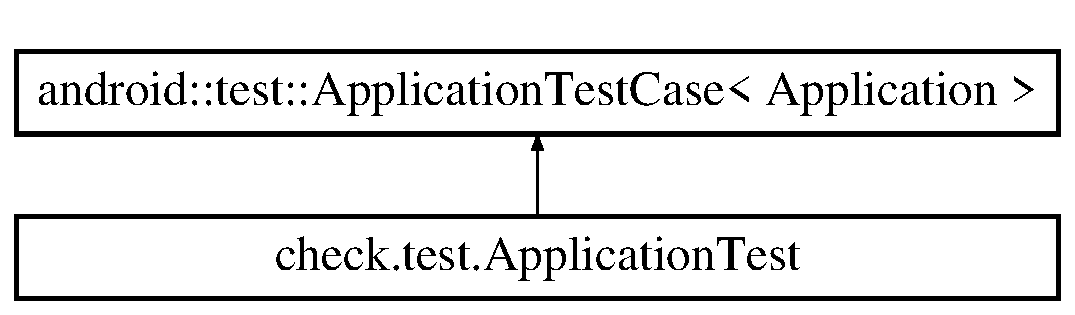
\includegraphics[height=2.000000cm]{classcheck_1_1test_1_1_application_test}
\end{center}
\end{figure}


\subsection{Detailed Description}
Testing Fundamentals. 

\href{http://d.android.com/tools/testing/testing_android.html}{\tt Testing Fundamentals} 

The documentation for this class was generated from the following file\+:\begin{DoxyCompactItemize}
\item 
C\+:/\+Users/\+Zwretched/.\+Android\+Studio1.\+4/\+Projects/\+Dress\+Me\+\_\+\+Android/\+Dress\+Me/src/android\+Test/java/check/test/Application\+Test.\+java\end{DoxyCompactItemize}

\hypertarget{classandroid_1_1support_1_1design_1_1_r_1_1attr}{}\section{android.\+support.\+design.\+R.\+attr Class Reference}
\label{classandroid_1_1support_1_1design_1_1_r_1_1attr}\index{android.\+support.\+design.\+R.\+attr@{android.\+support.\+design.\+R.\+attr}}
\subsection*{Static Public Attributes}
\begin{DoxyCompactItemize}
\item 
\hypertarget{classandroid_1_1support_1_1design_1_1_r_1_1attr_ae760bb3759dc75e0a49d12b13a525863}{}static final int {\bfseries action\+Bar\+Divider} = 0x7f01009b\label{classandroid_1_1support_1_1design_1_1_r_1_1attr_ae760bb3759dc75e0a49d12b13a525863}

\item 
\hypertarget{classandroid_1_1support_1_1design_1_1_r_1_1attr_a22428b19c7a60481d738d41421d2cae0}{}static final int {\bfseries action\+Bar\+Item\+Background} = 0x7f01009c\label{classandroid_1_1support_1_1design_1_1_r_1_1attr_a22428b19c7a60481d738d41421d2cae0}

\item 
\hypertarget{classandroid_1_1support_1_1design_1_1_r_1_1attr_a3099f3c0b99e3397da50683e55b24099}{}static final int {\bfseries action\+Bar\+Popup\+Theme} = 0x7f010095\label{classandroid_1_1support_1_1design_1_1_r_1_1attr_a3099f3c0b99e3397da50683e55b24099}

\item 
\hypertarget{classandroid_1_1support_1_1design_1_1_r_1_1attr_a3b80a59651b1b38d6c5497c22058009a}{}static final int {\bfseries action\+Bar\+Size} = 0x7f01009a\label{classandroid_1_1support_1_1design_1_1_r_1_1attr_a3b80a59651b1b38d6c5497c22058009a}

\item 
\hypertarget{classandroid_1_1support_1_1design_1_1_r_1_1attr_af3f9f00064ed4da503a855889da464de}{}static final int {\bfseries action\+Bar\+Split\+Style} = 0x7f010097\label{classandroid_1_1support_1_1design_1_1_r_1_1attr_af3f9f00064ed4da503a855889da464de}

\item 
\hypertarget{classandroid_1_1support_1_1design_1_1_r_1_1attr_afe4ac373c79d64575d48146ce16087f2}{}static final int {\bfseries action\+Bar\+Style} = 0x7f010096\label{classandroid_1_1support_1_1design_1_1_r_1_1attr_afe4ac373c79d64575d48146ce16087f2}

\item 
\hypertarget{classandroid_1_1support_1_1design_1_1_r_1_1attr_a2ca82a9598dc456d84aabd95ed349dc2}{}static final int {\bfseries action\+Bar\+Tab\+Bar\+Style} = 0x7f010091\label{classandroid_1_1support_1_1design_1_1_r_1_1attr_a2ca82a9598dc456d84aabd95ed349dc2}

\item 
\hypertarget{classandroid_1_1support_1_1design_1_1_r_1_1attr_a52b2ed4142fd2acadf605ff733a7443b}{}static final int {\bfseries action\+Bar\+Tab\+Style} = 0x7f010090\label{classandroid_1_1support_1_1design_1_1_r_1_1attr_a52b2ed4142fd2acadf605ff733a7443b}

\item 
\hypertarget{classandroid_1_1support_1_1design_1_1_r_1_1attr_ab794448e6906906fc9edb74109c3ad5e}{}static final int {\bfseries action\+Bar\+Tab\+Text\+Style} = 0x7f010092\label{classandroid_1_1support_1_1design_1_1_r_1_1attr_ab794448e6906906fc9edb74109c3ad5e}

\item 
\hypertarget{classandroid_1_1support_1_1design_1_1_r_1_1attr_a92eaedad4431dca9ec3d00edd8434ce2}{}static final int {\bfseries action\+Bar\+Theme} = 0x7f010098\label{classandroid_1_1support_1_1design_1_1_r_1_1attr_a92eaedad4431dca9ec3d00edd8434ce2}

\item 
\hypertarget{classandroid_1_1support_1_1design_1_1_r_1_1attr_af0baa7827e6e80093848731140dc46b6}{}static final int {\bfseries action\+Bar\+Widget\+Theme} = 0x7f010099\label{classandroid_1_1support_1_1design_1_1_r_1_1attr_af0baa7827e6e80093848731140dc46b6}

\item 
\hypertarget{classandroid_1_1support_1_1design_1_1_r_1_1attr_ab12d475fd7924195e1673ccc3d20e441}{}static final int {\bfseries action\+Button\+Style} = 0x7f0100b5\label{classandroid_1_1support_1_1design_1_1_r_1_1attr_ab12d475fd7924195e1673ccc3d20e441}

\item 
\hypertarget{classandroid_1_1support_1_1design_1_1_r_1_1attr_a6e485f83950c6df7a7fa7b58b7ce60f1}{}static final int {\bfseries action\+Drop\+Down\+Style} = 0x7f0100b1\label{classandroid_1_1support_1_1design_1_1_r_1_1attr_a6e485f83950c6df7a7fa7b58b7ce60f1}

\item 
\hypertarget{classandroid_1_1support_1_1design_1_1_r_1_1attr_ad538703779b49b42e926051d5937eb0f}{}static final int {\bfseries action\+Layout} = 0x7f01004f\label{classandroid_1_1support_1_1design_1_1_r_1_1attr_ad538703779b49b42e926051d5937eb0f}

\item 
\hypertarget{classandroid_1_1support_1_1design_1_1_r_1_1attr_a18a474dd4d75964fd29507f66ba20918}{}static final int {\bfseries action\+Menu\+Text\+Appearance} = 0x7f01009d\label{classandroid_1_1support_1_1design_1_1_r_1_1attr_a18a474dd4d75964fd29507f66ba20918}

\item 
\hypertarget{classandroid_1_1support_1_1design_1_1_r_1_1attr_a38bb816c17a2416113a223c4d476c7e5}{}static final int {\bfseries action\+Menu\+Text\+Color} = 0x7f01009e\label{classandroid_1_1support_1_1design_1_1_r_1_1attr_a38bb816c17a2416113a223c4d476c7e5}

\item 
\hypertarget{classandroid_1_1support_1_1design_1_1_r_1_1attr_abc52d011e78f0f7cd31d084707c826fc}{}static final int {\bfseries action\+Mode\+Background} = 0x7f0100a1\label{classandroid_1_1support_1_1design_1_1_r_1_1attr_abc52d011e78f0f7cd31d084707c826fc}

\item 
\hypertarget{classandroid_1_1support_1_1design_1_1_r_1_1attr_a389cd8e4c024d3acf65d8b5a3ccec912}{}static final int {\bfseries action\+Mode\+Close\+Button\+Style} = 0x7f0100a0\label{classandroid_1_1support_1_1design_1_1_r_1_1attr_a389cd8e4c024d3acf65d8b5a3ccec912}

\item 
\hypertarget{classandroid_1_1support_1_1design_1_1_r_1_1attr_a539705d65d41d03956688af3b083a80c}{}static final int {\bfseries action\+Mode\+Close\+Drawable} = 0x7f0100a3\label{classandroid_1_1support_1_1design_1_1_r_1_1attr_a539705d65d41d03956688af3b083a80c}

\item 
\hypertarget{classandroid_1_1support_1_1design_1_1_r_1_1attr_a9709f5fbcd7c014134e7440ba577ad29}{}static final int {\bfseries action\+Mode\+Copy\+Drawable} = 0x7f0100a5\label{classandroid_1_1support_1_1design_1_1_r_1_1attr_a9709f5fbcd7c014134e7440ba577ad29}

\item 
\hypertarget{classandroid_1_1support_1_1design_1_1_r_1_1attr_abdef737ac2e0d89e53de9d49ec74488f}{}static final int {\bfseries action\+Mode\+Cut\+Drawable} = 0x7f0100a4\label{classandroid_1_1support_1_1design_1_1_r_1_1attr_abdef737ac2e0d89e53de9d49ec74488f}

\item 
\hypertarget{classandroid_1_1support_1_1design_1_1_r_1_1attr_a75e6e720c7d37b501bb3b16d326ec282}{}static final int {\bfseries action\+Mode\+Find\+Drawable} = 0x7f0100a9\label{classandroid_1_1support_1_1design_1_1_r_1_1attr_a75e6e720c7d37b501bb3b16d326ec282}

\item 
\hypertarget{classandroid_1_1support_1_1design_1_1_r_1_1attr_afecf65fdc5c7b1990b9100f5078307a0}{}static final int {\bfseries action\+Mode\+Paste\+Drawable} = 0x7f0100a6\label{classandroid_1_1support_1_1design_1_1_r_1_1attr_afecf65fdc5c7b1990b9100f5078307a0}

\item 
\hypertarget{classandroid_1_1support_1_1design_1_1_r_1_1attr_a36582c93d9f5ca55e25c3f8913820b49}{}static final int {\bfseries action\+Mode\+Popup\+Window\+Style} = 0x7f0100ab\label{classandroid_1_1support_1_1design_1_1_r_1_1attr_a36582c93d9f5ca55e25c3f8913820b49}

\item 
\hypertarget{classandroid_1_1support_1_1design_1_1_r_1_1attr_ab2a713bb29967a97cd4d8bebfa65b9ba}{}static final int {\bfseries action\+Mode\+Select\+All\+Drawable} = 0x7f0100a7\label{classandroid_1_1support_1_1design_1_1_r_1_1attr_ab2a713bb29967a97cd4d8bebfa65b9ba}

\item 
\hypertarget{classandroid_1_1support_1_1design_1_1_r_1_1attr_aaf7fd84ea5fbf46843fca2dd2376d8da}{}static final int {\bfseries action\+Mode\+Share\+Drawable} = 0x7f0100a8\label{classandroid_1_1support_1_1design_1_1_r_1_1attr_aaf7fd84ea5fbf46843fca2dd2376d8da}

\item 
\hypertarget{classandroid_1_1support_1_1design_1_1_r_1_1attr_a063adaf7bf2aedb313fccd7c9c406286}{}static final int {\bfseries action\+Mode\+Split\+Background} = 0x7f0100a2\label{classandroid_1_1support_1_1design_1_1_r_1_1attr_a063adaf7bf2aedb313fccd7c9c406286}

\item 
\hypertarget{classandroid_1_1support_1_1design_1_1_r_1_1attr_ac448239603f330b08cc4a76a2d01704d}{}static final int {\bfseries action\+Mode\+Style} = 0x7f01009f\label{classandroid_1_1support_1_1design_1_1_r_1_1attr_ac448239603f330b08cc4a76a2d01704d}

\item 
\hypertarget{classandroid_1_1support_1_1design_1_1_r_1_1attr_a738dea168ce0bf399bfe38eccce9b38e}{}static final int {\bfseries action\+Mode\+Web\+Search\+Drawable} = 0x7f0100aa\label{classandroid_1_1support_1_1design_1_1_r_1_1attr_a738dea168ce0bf399bfe38eccce9b38e}

\item 
\hypertarget{classandroid_1_1support_1_1design_1_1_r_1_1attr_ad924f1960d613f38bbea6490e7bafac3}{}static final int {\bfseries action\+Overflow\+Button\+Style} = 0x7f010093\label{classandroid_1_1support_1_1design_1_1_r_1_1attr_ad924f1960d613f38bbea6490e7bafac3}

\item 
\hypertarget{classandroid_1_1support_1_1design_1_1_r_1_1attr_ab8ba6f67460fb8b21432c3855ba1dc3b}{}static final int {\bfseries action\+Overflow\+Menu\+Style} = 0x7f010094\label{classandroid_1_1support_1_1design_1_1_r_1_1attr_ab8ba6f67460fb8b21432c3855ba1dc3b}

\item 
\hypertarget{classandroid_1_1support_1_1design_1_1_r_1_1attr_ace4d4f4767149f10652ae11fa37ba6b4}{}static final int {\bfseries action\+Provider\+Class} = 0x7f010051\label{classandroid_1_1support_1_1design_1_1_r_1_1attr_ace4d4f4767149f10652ae11fa37ba6b4}

\item 
\hypertarget{classandroid_1_1support_1_1design_1_1_r_1_1attr_afa305c5b28100674d981f2d3159f14fe}{}static final int {\bfseries action\+View\+Class} = 0x7f010050\label{classandroid_1_1support_1_1design_1_1_r_1_1attr_afa305c5b28100674d981f2d3159f14fe}

\item 
\hypertarget{classandroid_1_1support_1_1design_1_1_r_1_1attr_a772f9b819db28308273b08c1e3927173}{}static final int {\bfseries activity\+Chooser\+View\+Style} = 0x7f0100bd\label{classandroid_1_1support_1_1design_1_1_r_1_1attr_a772f9b819db28308273b08c1e3927173}

\item 
\hypertarget{classandroid_1_1support_1_1design_1_1_r_1_1attr_af6b9ec9b563431092df394acb9ab9d3a}{}static final int {\bfseries alert\+Dialog\+Button\+Group\+Style} = 0x7f0100df\label{classandroid_1_1support_1_1design_1_1_r_1_1attr_af6b9ec9b563431092df394acb9ab9d3a}

\item 
\hypertarget{classandroid_1_1support_1_1design_1_1_r_1_1attr_a0fe920d2f800df2ca3cb9f9c78b5a63d}{}static final int {\bfseries alert\+Dialog\+Center\+Buttons} = 0x7f0100e0\label{classandroid_1_1support_1_1design_1_1_r_1_1attr_a0fe920d2f800df2ca3cb9f9c78b5a63d}

\item 
\hypertarget{classandroid_1_1support_1_1design_1_1_r_1_1attr_a243018b6844b3078db89b7739f73fc13}{}static final int {\bfseries alert\+Dialog\+Style} = 0x7f0100de\label{classandroid_1_1support_1_1design_1_1_r_1_1attr_a243018b6844b3078db89b7739f73fc13}

\item 
\hypertarget{classandroid_1_1support_1_1design_1_1_r_1_1attr_a544216476a21a3edafffc422db18bf9f}{}static final int {\bfseries alert\+Dialog\+Theme} = 0x7f0100e1\label{classandroid_1_1support_1_1design_1_1_r_1_1attr_a544216476a21a3edafffc422db18bf9f}

\item 
\hypertarget{classandroid_1_1support_1_1design_1_1_r_1_1attr_a1c5413c1d098f1dedeec52bf1f60bbd4}{}static final int {\bfseries arrow\+Head\+Length} = 0x7f010043\label{classandroid_1_1support_1_1design_1_1_r_1_1attr_a1c5413c1d098f1dedeec52bf1f60bbd4}

\item 
\hypertarget{classandroid_1_1support_1_1design_1_1_r_1_1attr_a5173098b8b4a2a042d1dc65c0726feb4}{}static final int {\bfseries arrow\+Shaft\+Length} = 0x7f010044\label{classandroid_1_1support_1_1design_1_1_r_1_1attr_a5173098b8b4a2a042d1dc65c0726feb4}

\item 
\hypertarget{classandroid_1_1support_1_1design_1_1_r_1_1attr_a7b3906d45193c214e16185415dde30b0}{}static final int {\bfseries auto\+Complete\+Text\+View\+Style} = 0x7f0100e6\label{classandroid_1_1support_1_1design_1_1_r_1_1attr_a7b3906d45193c214e16185415dde30b0}

\item 
\hypertarget{classandroid_1_1support_1_1design_1_1_r_1_1attr_a633e86200cd9774275242631c63985ee}{}static final int {\bfseries background} = 0x7f01000c\label{classandroid_1_1support_1_1design_1_1_r_1_1attr_a633e86200cd9774275242631c63985ee}

\item 
\hypertarget{classandroid_1_1support_1_1design_1_1_r_1_1attr_ac7943a5fbb475fbbfe90e0a5a6622afb}{}static final int {\bfseries background\+Split} = 0x7f01000e\label{classandroid_1_1support_1_1design_1_1_r_1_1attr_ac7943a5fbb475fbbfe90e0a5a6622afb}

\item 
\hypertarget{classandroid_1_1support_1_1design_1_1_r_1_1attr_a67ec9129f83e25973c54736f26ebb03b}{}static final int {\bfseries background\+Stacked} = 0x7f01000d\label{classandroid_1_1support_1_1design_1_1_r_1_1attr_a67ec9129f83e25973c54736f26ebb03b}

\item 
\hypertarget{classandroid_1_1support_1_1design_1_1_r_1_1attr_aa714e7de34a4c22bd4a43350611f6424}{}static final int {\bfseries background\+Tint} = 0x7f010102\label{classandroid_1_1support_1_1design_1_1_r_1_1attr_aa714e7de34a4c22bd4a43350611f6424}

\item 
\hypertarget{classandroid_1_1support_1_1design_1_1_r_1_1attr_a5c4554ea65007751ccc0078bde491065}{}static final int {\bfseries background\+Tint\+Mode} = 0x7f010103\label{classandroid_1_1support_1_1design_1_1_r_1_1attr_a5c4554ea65007751ccc0078bde491065}

\item 
\hypertarget{classandroid_1_1support_1_1design_1_1_r_1_1attr_aed76efd8f3192670d26289e5d1a6a94e}{}static final int {\bfseries bar\+Length} = 0x7f010045\label{classandroid_1_1support_1_1design_1_1_r_1_1attr_aed76efd8f3192670d26289e5d1a6a94e}

\item 
\hypertarget{classandroid_1_1support_1_1design_1_1_r_1_1attr_a6bd3a8ada6445384f29a7b94a7679090}{}static final int {\bfseries behavior\+\_\+overlap\+Top} = 0x7f01005c\label{classandroid_1_1support_1_1design_1_1_r_1_1attr_a6bd3a8ada6445384f29a7b94a7679090}

\item 
\hypertarget{classandroid_1_1support_1_1design_1_1_r_1_1attr_a0b9b9703ae190c90c9130ba940edfe1a}{}static final int {\bfseries border\+Width} = 0x7f01004a\label{classandroid_1_1support_1_1design_1_1_r_1_1attr_a0b9b9703ae190c90c9130ba940edfe1a}

\item 
\hypertarget{classandroid_1_1support_1_1design_1_1_r_1_1attr_af2eab970fb1e3e757b04a40b2552d82e}{}static final int {\bfseries borderless\+Button\+Style} = 0x7f0100ba\label{classandroid_1_1support_1_1design_1_1_r_1_1attr_af2eab970fb1e3e757b04a40b2552d82e}

\item 
\hypertarget{classandroid_1_1support_1_1design_1_1_r_1_1attr_a3a9d5900929a564d36943910be6f5f8e}{}static final int {\bfseries button\+Bar\+Button\+Style} = 0x7f0100b7\label{classandroid_1_1support_1_1design_1_1_r_1_1attr_a3a9d5900929a564d36943910be6f5f8e}

\item 
\hypertarget{classandroid_1_1support_1_1design_1_1_r_1_1attr_ad684421bc3fb71c6503b0b9a0ba2474b}{}static final int {\bfseries button\+Bar\+Negative\+Button\+Style} = 0x7f0100e4\label{classandroid_1_1support_1_1design_1_1_r_1_1attr_ad684421bc3fb71c6503b0b9a0ba2474b}

\item 
\hypertarget{classandroid_1_1support_1_1design_1_1_r_1_1attr_af941874bd15ba48802fe339d3aed2e67}{}static final int {\bfseries button\+Bar\+Neutral\+Button\+Style} = 0x7f0100e5\label{classandroid_1_1support_1_1design_1_1_r_1_1attr_af941874bd15ba48802fe339d3aed2e67}

\item 
\hypertarget{classandroid_1_1support_1_1design_1_1_r_1_1attr_adfdaff8d5b88aedcb767a3d361b26536}{}static final int {\bfseries button\+Bar\+Positive\+Button\+Style} = 0x7f0100e3\label{classandroid_1_1support_1_1design_1_1_r_1_1attr_adfdaff8d5b88aedcb767a3d361b26536}

\item 
\hypertarget{classandroid_1_1support_1_1design_1_1_r_1_1attr_aa0cd4b2b184796faaa8598d7d55a1980}{}static final int {\bfseries button\+Bar\+Style} = 0x7f0100b6\label{classandroid_1_1support_1_1design_1_1_r_1_1attr_aa0cd4b2b184796faaa8598d7d55a1980}

\item 
\hypertarget{classandroid_1_1support_1_1design_1_1_r_1_1attr_af8a569d126f3f38713edd8c55471112d}{}static final int {\bfseries button\+Panel\+Side\+Layout} = 0x7f01001f\label{classandroid_1_1support_1_1design_1_1_r_1_1attr_af8a569d126f3f38713edd8c55471112d}

\item 
\hypertarget{classandroid_1_1support_1_1design_1_1_r_1_1attr_af811016b90d459ec8303bdee577b3bbe}{}static final int {\bfseries button\+Style} = 0x7f0100e7\label{classandroid_1_1support_1_1design_1_1_r_1_1attr_af811016b90d459ec8303bdee577b3bbe}

\item 
\hypertarget{classandroid_1_1support_1_1design_1_1_r_1_1attr_a6229dc8c52c9cb2bb1b60ae629a23df8}{}static final int {\bfseries button\+Style\+Small} = 0x7f0100e8\label{classandroid_1_1support_1_1design_1_1_r_1_1attr_a6229dc8c52c9cb2bb1b60ae629a23df8}

\item 
\hypertarget{classandroid_1_1support_1_1design_1_1_r_1_1attr_a481984709e9647ce5d7948243edfe917}{}static final int {\bfseries button\+Tint} = 0x7f010037\label{classandroid_1_1support_1_1design_1_1_r_1_1attr_a481984709e9647ce5d7948243edfe917}

\item 
\hypertarget{classandroid_1_1support_1_1design_1_1_r_1_1attr_a47b2fd06b59f201a643295986397e47a}{}static final int {\bfseries button\+Tint\+Mode} = 0x7f010038\label{classandroid_1_1support_1_1design_1_1_r_1_1attr_a47b2fd06b59f201a643295986397e47a}

\item 
\hypertarget{classandroid_1_1support_1_1design_1_1_r_1_1attr_abac68647b3bf87f91a6a8797daa07430}{}static final int {\bfseries checkbox\+Style} = 0x7f0100e9\label{classandroid_1_1support_1_1design_1_1_r_1_1attr_abac68647b3bf87f91a6a8797daa07430}

\item 
\hypertarget{classandroid_1_1support_1_1design_1_1_r_1_1attr_a46619b29955b955344296891b92bfc16}{}static final int {\bfseries checked\+Text\+View\+Style} = 0x7f0100ea\label{classandroid_1_1support_1_1design_1_1_r_1_1attr_a46619b29955b955344296891b92bfc16}

\item 
\hypertarget{classandroid_1_1support_1_1design_1_1_r_1_1attr_ab8fd66b58592da0068302a1f8a189f7c}{}static final int {\bfseries close\+Icon} = 0x7f010061\label{classandroid_1_1support_1_1design_1_1_r_1_1attr_ab8fd66b58592da0068302a1f8a189f7c}

\item 
\hypertarget{classandroid_1_1support_1_1design_1_1_r_1_1attr_afe89b1d611a683ea18f85ffdb515f2e0}{}static final int {\bfseries close\+Item\+Layout} = 0x7f01001c\label{classandroid_1_1support_1_1design_1_1_r_1_1attr_afe89b1d611a683ea18f85ffdb515f2e0}

\item 
\hypertarget{classandroid_1_1support_1_1design_1_1_r_1_1attr_a215609776fda25e73da2d429d4e8310f}{}static final int {\bfseries collapse\+Content\+Description} = 0x7f0100f9\label{classandroid_1_1support_1_1design_1_1_r_1_1attr_a215609776fda25e73da2d429d4e8310f}

\item 
\hypertarget{classandroid_1_1support_1_1design_1_1_r_1_1attr_a8f6c4abc219435477139c0be490cc35c}{}static final int {\bfseries collapse\+Icon} = 0x7f0100f8\label{classandroid_1_1support_1_1design_1_1_r_1_1attr_a8f6c4abc219435477139c0be490cc35c}

\item 
\hypertarget{classandroid_1_1support_1_1design_1_1_r_1_1attr_a2f6e7d8594fc1d351255f9c547a25e5e}{}static final int {\bfseries collapsed\+Title\+Gravity} = 0x7f010034\label{classandroid_1_1support_1_1design_1_1_r_1_1attr_a2f6e7d8594fc1d351255f9c547a25e5e}

\item 
\hypertarget{classandroid_1_1support_1_1design_1_1_r_1_1attr_a4d0eb85ec9562313f00d4af6c9ed6b73}{}static final int {\bfseries collapsed\+Title\+Text\+Appearance} = 0x7f010030\label{classandroid_1_1support_1_1design_1_1_r_1_1attr_a4d0eb85ec9562313f00d4af6c9ed6b73}

\item 
\hypertarget{classandroid_1_1support_1_1design_1_1_r_1_1attr_ab11a93bf8eba02b9dcc4fd0f690cbc73}{}static final int {\bfseries color} = 0x7f01003f\label{classandroid_1_1support_1_1design_1_1_r_1_1attr_ab11a93bf8eba02b9dcc4fd0f690cbc73}

\item 
\hypertarget{classandroid_1_1support_1_1design_1_1_r_1_1attr_a15e1522787f101529fbfb34e6839a47e}{}static final int {\bfseries color\+Accent} = 0x7f0100d7\label{classandroid_1_1support_1_1design_1_1_r_1_1attr_a15e1522787f101529fbfb34e6839a47e}

\item 
\hypertarget{classandroid_1_1support_1_1design_1_1_r_1_1attr_af13a0f02cf3973a6702c3aed33502dca}{}static final int {\bfseries color\+Button\+Normal} = 0x7f0100db\label{classandroid_1_1support_1_1design_1_1_r_1_1attr_af13a0f02cf3973a6702c3aed33502dca}

\item 
\hypertarget{classandroid_1_1support_1_1design_1_1_r_1_1attr_afe306e82da2093e0461e14011062f6d0}{}static final int {\bfseries color\+Control\+Activated} = 0x7f0100d9\label{classandroid_1_1support_1_1design_1_1_r_1_1attr_afe306e82da2093e0461e14011062f6d0}

\item 
\hypertarget{classandroid_1_1support_1_1design_1_1_r_1_1attr_a9b9ac1ed1cd6476e66fbf585519be242}{}static final int {\bfseries color\+Control\+Highlight} = 0x7f0100da\label{classandroid_1_1support_1_1design_1_1_r_1_1attr_a9b9ac1ed1cd6476e66fbf585519be242}

\item 
\hypertarget{classandroid_1_1support_1_1design_1_1_r_1_1attr_a90e1ede923ec8393bd6f1a3218f9836b}{}static final int {\bfseries color\+Control\+Normal} = 0x7f0100d8\label{classandroid_1_1support_1_1design_1_1_r_1_1attr_a90e1ede923ec8393bd6f1a3218f9836b}

\item 
\hypertarget{classandroid_1_1support_1_1design_1_1_r_1_1attr_ae16c90f75dbb495b67dbcc7d3b2d5875}{}static final int {\bfseries color\+Primary} = 0x7f0100d5\label{classandroid_1_1support_1_1design_1_1_r_1_1attr_ae16c90f75dbb495b67dbcc7d3b2d5875}

\item 
\hypertarget{classandroid_1_1support_1_1design_1_1_r_1_1attr_a03a2e86e19456d190709fd13c9245eff}{}static final int {\bfseries color\+Primary\+Dark} = 0x7f0100d6\label{classandroid_1_1support_1_1design_1_1_r_1_1attr_a03a2e86e19456d190709fd13c9245eff}

\item 
\hypertarget{classandroid_1_1support_1_1design_1_1_r_1_1attr_a079f7b1cfe50d26938aeeea1cd78e6ad}{}static final int {\bfseries color\+Switch\+Thumb\+Normal} = 0x7f0100dc\label{classandroid_1_1support_1_1design_1_1_r_1_1attr_a079f7b1cfe50d26938aeeea1cd78e6ad}

\item 
\hypertarget{classandroid_1_1support_1_1design_1_1_r_1_1attr_a11bbc63f864f8a93e51e41de4ed8cb1b}{}static final int {\bfseries commit\+Icon} = 0x7f010066\label{classandroid_1_1support_1_1design_1_1_r_1_1attr_a11bbc63f864f8a93e51e41de4ed8cb1b}

\item 
\hypertarget{classandroid_1_1support_1_1design_1_1_r_1_1attr_ade46dc0fa819b1068e4a9914ae7e17ea}{}static final int {\bfseries content\+Inset\+End} = 0x7f010017\label{classandroid_1_1support_1_1design_1_1_r_1_1attr_ade46dc0fa819b1068e4a9914ae7e17ea}

\item 
\hypertarget{classandroid_1_1support_1_1design_1_1_r_1_1attr_a8de8b60fcce084326706615ffa0eb7fe}{}static final int {\bfseries content\+Inset\+Left} = 0x7f010018\label{classandroid_1_1support_1_1design_1_1_r_1_1attr_a8de8b60fcce084326706615ffa0eb7fe}

\item 
\hypertarget{classandroid_1_1support_1_1design_1_1_r_1_1attr_aecf3f2220db7da109fc27bc18b181056}{}static final int {\bfseries content\+Inset\+Right} = 0x7f010019\label{classandroid_1_1support_1_1design_1_1_r_1_1attr_aecf3f2220db7da109fc27bc18b181056}

\item 
\hypertarget{classandroid_1_1support_1_1design_1_1_r_1_1attr_a77f9dfd9dce9f6c88ca65515c38cdc14}{}static final int {\bfseries content\+Inset\+Start} = 0x7f010016\label{classandroid_1_1support_1_1design_1_1_r_1_1attr_a77f9dfd9dce9f6c88ca65515c38cdc14}

\item 
\hypertarget{classandroid_1_1support_1_1design_1_1_r_1_1attr_aa8a14d5b4064a43c901ed8f487694a90}{}static final int {\bfseries content\+Scrim} = 0x7f010031\label{classandroid_1_1support_1_1design_1_1_r_1_1attr_aa8a14d5b4064a43c901ed8f487694a90}

\item 
\hypertarget{classandroid_1_1support_1_1design_1_1_r_1_1attr_aa9c8ead3946ee0ead67bb68d1108f94a}{}static final int {\bfseries control\+Background} = 0x7f0100dd\label{classandroid_1_1support_1_1design_1_1_r_1_1attr_aa9c8ead3946ee0ead67bb68d1108f94a}

\item 
\hypertarget{classandroid_1_1support_1_1design_1_1_r_1_1attr_a547b2301cd4621ac6ea5496b9664a48a}{}static final int {\bfseries custom\+Navigation\+Layout} = 0x7f01000f\label{classandroid_1_1support_1_1design_1_1_r_1_1attr_a547b2301cd4621ac6ea5496b9664a48a}

\item 
\hypertarget{classandroid_1_1support_1_1design_1_1_r_1_1attr_acaec52b5bbfc9784046add642d100758}{}static final int {\bfseries default\+Query\+Hint} = 0x7f010060\label{classandroid_1_1support_1_1design_1_1_r_1_1attr_acaec52b5bbfc9784046add642d100758}

\item 
\hypertarget{classandroid_1_1support_1_1design_1_1_r_1_1attr_a9fa2a0152120967429584cb510c55ef2}{}static final int {\bfseries dialog\+Preferred\+Padding} = 0x7f0100af\label{classandroid_1_1support_1_1design_1_1_r_1_1attr_a9fa2a0152120967429584cb510c55ef2}

\item 
\hypertarget{classandroid_1_1support_1_1design_1_1_r_1_1attr_a591c5c254647c58b1ce1ab9dff81f91a}{}static final int {\bfseries dialog\+Theme} = 0x7f0100ae\label{classandroid_1_1support_1_1design_1_1_r_1_1attr_a591c5c254647c58b1ce1ab9dff81f91a}

\item 
\hypertarget{classandroid_1_1support_1_1design_1_1_r_1_1attr_a93c1aae4701355ebdf9580afa1586c65}{}static final int {\bfseries display\+Options} = 0x7f010005\label{classandroid_1_1support_1_1design_1_1_r_1_1attr_a93c1aae4701355ebdf9580afa1586c65}

\item 
\hypertarget{classandroid_1_1support_1_1design_1_1_r_1_1attr_ae104d6437ed6e2bcdf6d19e7512c698f}{}static final int {\bfseries divider} = 0x7f01000b\label{classandroid_1_1support_1_1design_1_1_r_1_1attr_ae104d6437ed6e2bcdf6d19e7512c698f}

\item 
\hypertarget{classandroid_1_1support_1_1design_1_1_r_1_1attr_a5c3d002a620e4a91207c532d94baff2e}{}static final int {\bfseries divider\+Horizontal} = 0x7f0100bc\label{classandroid_1_1support_1_1design_1_1_r_1_1attr_a5c3d002a620e4a91207c532d94baff2e}

\item 
\hypertarget{classandroid_1_1support_1_1design_1_1_r_1_1attr_aa232cfdd1a85b48a7020e02ae3feaaca}{}static final int {\bfseries divider\+Padding} = 0x7f01004d\label{classandroid_1_1support_1_1design_1_1_r_1_1attr_aa232cfdd1a85b48a7020e02ae3feaaca}

\item 
\hypertarget{classandroid_1_1support_1_1design_1_1_r_1_1attr_ad9bff20984b9b305919aaf3b1a699315}{}static final int {\bfseries divider\+Vertical} = 0x7f0100bb\label{classandroid_1_1support_1_1design_1_1_r_1_1attr_ad9bff20984b9b305919aaf3b1a699315}

\item 
\hypertarget{classandroid_1_1support_1_1design_1_1_r_1_1attr_a752d7489bf25759f26da0de7051c6d6c}{}static final int {\bfseries drawable\+Size} = 0x7f010041\label{classandroid_1_1support_1_1design_1_1_r_1_1attr_a752d7489bf25759f26da0de7051c6d6c}

\item 
\hypertarget{classandroid_1_1support_1_1design_1_1_r_1_1attr_a067fc22595374f6cf79df43697f707d0}{}static final int {\bfseries drawer\+Arrow\+Style} = 0x7f010000\label{classandroid_1_1support_1_1design_1_1_r_1_1attr_a067fc22595374f6cf79df43697f707d0}

\item 
\hypertarget{classandroid_1_1support_1_1design_1_1_r_1_1attr_aecae50e199b147d3412c64228e7ffbfa}{}static final int {\bfseries drop\+Down\+List\+View\+Style} = 0x7f0100cd\label{classandroid_1_1support_1_1design_1_1_r_1_1attr_aecae50e199b147d3412c64228e7ffbfa}

\item 
\hypertarget{classandroid_1_1support_1_1design_1_1_r_1_1attr_a9771b11e6d5d4f3ac5339bfa4afb5bdf}{}static final int {\bfseries dropdown\+List\+Preferred\+Item\+Height} = 0x7f0100b2\label{classandroid_1_1support_1_1design_1_1_r_1_1attr_a9771b11e6d5d4f3ac5339bfa4afb5bdf}

\item 
\hypertarget{classandroid_1_1support_1_1design_1_1_r_1_1attr_ae5151ecdcfbdc46e6e424c79b60548ee}{}static final int {\bfseries edit\+Text\+Background} = 0x7f0100c3\label{classandroid_1_1support_1_1design_1_1_r_1_1attr_ae5151ecdcfbdc46e6e424c79b60548ee}

\item 
\hypertarget{classandroid_1_1support_1_1design_1_1_r_1_1attr_ae5bffd7d1a0defcc8af0a2d675908267}{}static final int {\bfseries edit\+Text\+Color} = 0x7f0100c2\label{classandroid_1_1support_1_1design_1_1_r_1_1attr_ae5bffd7d1a0defcc8af0a2d675908267}

\item 
\hypertarget{classandroid_1_1support_1_1design_1_1_r_1_1attr_ac21901da73b034db7da8b6598b5954a5}{}static final int {\bfseries edit\+Text\+Style} = 0x7f0100eb\label{classandroid_1_1support_1_1design_1_1_r_1_1attr_ac21901da73b034db7da8b6598b5954a5}

\item 
\hypertarget{classandroid_1_1support_1_1design_1_1_r_1_1attr_a32597814963a4ec5dd120c66e7ac7f15}{}static final int {\bfseries elevation} = 0x7f01001a\label{classandroid_1_1support_1_1design_1_1_r_1_1attr_a32597814963a4ec5dd120c66e7ac7f15}

\item 
\hypertarget{classandroid_1_1support_1_1design_1_1_r_1_1attr_a33177626e9eac6ee0f334023420ed888}{}static final int {\bfseries error\+Enabled} = 0x7f010083\label{classandroid_1_1support_1_1design_1_1_r_1_1attr_a33177626e9eac6ee0f334023420ed888}

\item 
\hypertarget{classandroid_1_1support_1_1design_1_1_r_1_1attr_aff80f59fbd99ca8b22758a04767ac7d5}{}static final int {\bfseries error\+Text\+Appearance} = 0x7f010084\label{classandroid_1_1support_1_1design_1_1_r_1_1attr_aff80f59fbd99ca8b22758a04767ac7d5}

\item 
\hypertarget{classandroid_1_1support_1_1design_1_1_r_1_1attr_a294fef173d17119d81a2a22e1b059994}{}static final int {\bfseries expand\+Activity\+Overflow\+Button\+Drawable} = 0x7f01001e\label{classandroid_1_1support_1_1design_1_1_r_1_1attr_a294fef173d17119d81a2a22e1b059994}

\item 
\hypertarget{classandroid_1_1support_1_1design_1_1_r_1_1attr_a8b2f1952a1f1858370c55b77a5c8fdf0}{}static final int {\bfseries expanded} = 0x7f010024\label{classandroid_1_1support_1_1design_1_1_r_1_1attr_a8b2f1952a1f1858370c55b77a5c8fdf0}

\item 
\hypertarget{classandroid_1_1support_1_1design_1_1_r_1_1attr_af9227f3d0dd94b70bf8560495793ef46}{}static final int {\bfseries expanded\+Title\+Gravity} = 0x7f010035\label{classandroid_1_1support_1_1design_1_1_r_1_1attr_af9227f3d0dd94b70bf8560495793ef46}

\item 
\hypertarget{classandroid_1_1support_1_1design_1_1_r_1_1attr_aa82f302d274ae27a8c9353fadca028c8}{}static final int {\bfseries expanded\+Title\+Margin} = 0x7f01002a\label{classandroid_1_1support_1_1design_1_1_r_1_1attr_aa82f302d274ae27a8c9353fadca028c8}

\item 
\hypertarget{classandroid_1_1support_1_1design_1_1_r_1_1attr_a3eab7e6efce6d1e0bab6faf32ed77c76}{}static final int {\bfseries expanded\+Title\+Margin\+Bottom} = 0x7f01002e\label{classandroid_1_1support_1_1design_1_1_r_1_1attr_a3eab7e6efce6d1e0bab6faf32ed77c76}

\item 
\hypertarget{classandroid_1_1support_1_1design_1_1_r_1_1attr_ad547616c8f37d753a16d55b3af437504}{}static final int {\bfseries expanded\+Title\+Margin\+End} = 0x7f01002d\label{classandroid_1_1support_1_1design_1_1_r_1_1attr_ad547616c8f37d753a16d55b3af437504}

\item 
\hypertarget{classandroid_1_1support_1_1design_1_1_r_1_1attr_a117547f2f75572ed87f35bf8d2174c3c}{}static final int {\bfseries expanded\+Title\+Margin\+Start} = 0x7f01002b\label{classandroid_1_1support_1_1design_1_1_r_1_1attr_a117547f2f75572ed87f35bf8d2174c3c}

\item 
\hypertarget{classandroid_1_1support_1_1design_1_1_r_1_1attr_ab480074094d112513cccb460ca7d08ce}{}static final int {\bfseries expanded\+Title\+Margin\+Top} = 0x7f01002c\label{classandroid_1_1support_1_1design_1_1_r_1_1attr_ab480074094d112513cccb460ca7d08ce}

\item 
\hypertarget{classandroid_1_1support_1_1design_1_1_r_1_1attr_a0093d7cf21b5718aa96f111e023ca986}{}static final int {\bfseries expanded\+Title\+Text\+Appearance} = 0x7f01002f\label{classandroid_1_1support_1_1design_1_1_r_1_1attr_a0093d7cf21b5718aa96f111e023ca986}

\item 
\hypertarget{classandroid_1_1support_1_1design_1_1_r_1_1attr_ae50af000a6d2566abf822dd923f0e6bc}{}static final int {\bfseries fab\+Size} = 0x7f010048\label{classandroid_1_1support_1_1design_1_1_r_1_1attr_ae50af000a6d2566abf822dd923f0e6bc}

\item 
\hypertarget{classandroid_1_1support_1_1design_1_1_r_1_1attr_af5aa83bca46ec78627ca7af277ace09a}{}static final int {\bfseries gap\+Between\+Bars} = 0x7f010042\label{classandroid_1_1support_1_1design_1_1_r_1_1attr_af5aa83bca46ec78627ca7af277ace09a}

\item 
\hypertarget{classandroid_1_1support_1_1design_1_1_r_1_1attr_ab0832bfcb7a264b7f160a92f19c26514}{}static final int {\bfseries go\+Icon} = 0x7f010062\label{classandroid_1_1support_1_1design_1_1_r_1_1attr_ab0832bfcb7a264b7f160a92f19c26514}

\item 
\hypertarget{classandroid_1_1support_1_1design_1_1_r_1_1attr_a669a14ce772e913e335a7e450b199e21}{}static final int {\bfseries header\+Layout} = 0x7f010058\label{classandroid_1_1support_1_1design_1_1_r_1_1attr_a669a14ce772e913e335a7e450b199e21}

\item 
\hypertarget{classandroid_1_1support_1_1design_1_1_r_1_1attr_a67de67e33346463b7e8ccac5a5c3d2b8}{}static final int {\bfseries height} = 0x7f010001\label{classandroid_1_1support_1_1design_1_1_r_1_1attr_a67de67e33346463b7e8ccac5a5c3d2b8}

\item 
\hypertarget{classandroid_1_1support_1_1design_1_1_r_1_1attr_afad42994576791dcb844b6d5a92b106e}{}static final int {\bfseries hide\+On\+Content\+Scroll} = 0x7f010015\label{classandroid_1_1support_1_1design_1_1_r_1_1attr_afad42994576791dcb844b6d5a92b106e}

\item 
\hypertarget{classandroid_1_1support_1_1design_1_1_r_1_1attr_a45965840ce51b3dc10db2c5ed7c0d923}{}static final int {\bfseries hint\+Animation\+Enabled} = 0x7f010085\label{classandroid_1_1support_1_1design_1_1_r_1_1attr_a45965840ce51b3dc10db2c5ed7c0d923}

\item 
\hypertarget{classandroid_1_1support_1_1design_1_1_r_1_1attr_a571b12c480a0e39c924235a502df4a7a}{}static final int {\bfseries hint\+Text\+Appearance} = 0x7f010082\label{classandroid_1_1support_1_1design_1_1_r_1_1attr_a571b12c480a0e39c924235a502df4a7a}

\item 
\hypertarget{classandroid_1_1support_1_1design_1_1_r_1_1attr_a2cd44aad7205648aa1db17d8376012c7}{}static final int {\bfseries home\+As\+Up\+Indicator} = 0x7f0100b4\label{classandroid_1_1support_1_1design_1_1_r_1_1attr_a2cd44aad7205648aa1db17d8376012c7}

\item 
\hypertarget{classandroid_1_1support_1_1design_1_1_r_1_1attr_af4fde3588c8e7ef225a4babe99fb6327}{}static final int {\bfseries home\+Layout} = 0x7f010010\label{classandroid_1_1support_1_1design_1_1_r_1_1attr_af4fde3588c8e7ef225a4babe99fb6327}

\item 
\hypertarget{classandroid_1_1support_1_1design_1_1_r_1_1attr_a3dd29517b74c4eefbf204f5f85f3788e}{}static final int {\bfseries icon} = 0x7f010009\label{classandroid_1_1support_1_1design_1_1_r_1_1attr_a3dd29517b74c4eefbf204f5f85f3788e}

\item 
\hypertarget{classandroid_1_1support_1_1design_1_1_r_1_1attr_af56e63f7366c9cd5ce1c639e20df1369}{}static final int {\bfseries iconified\+By\+Default} = 0x7f01005e\label{classandroid_1_1support_1_1design_1_1_r_1_1attr_af56e63f7366c9cd5ce1c639e20df1369}

\item 
\hypertarget{classandroid_1_1support_1_1design_1_1_r_1_1attr_acf61552a40e127dc18fd4fb54c1eab8c}{}static final int {\bfseries indeterminate\+Progress\+Style} = 0x7f010012\label{classandroid_1_1support_1_1design_1_1_r_1_1attr_acf61552a40e127dc18fd4fb54c1eab8c}

\item 
\hypertarget{classandroid_1_1support_1_1design_1_1_r_1_1attr_ac1527e93f4ac647fe8b997a212e62754}{}static final int {\bfseries initial\+Activity\+Count} = 0x7f01001d\label{classandroid_1_1support_1_1design_1_1_r_1_1attr_ac1527e93f4ac647fe8b997a212e62754}

\item 
\hypertarget{classandroid_1_1support_1_1design_1_1_r_1_1attr_a54280b38c1851ec6e215016b464d32c2}{}static final int {\bfseries inset\+Foreground} = 0x7f01005b\label{classandroid_1_1support_1_1design_1_1_r_1_1attr_a54280b38c1851ec6e215016b464d32c2}

\item 
\hypertarget{classandroid_1_1support_1_1design_1_1_r_1_1attr_a1f68ce8ebcae8b5f8d8580fbffaabd82}{}static final int {\bfseries is\+Light\+Theme} = 0x7f010002\label{classandroid_1_1support_1_1design_1_1_r_1_1attr_a1f68ce8ebcae8b5f8d8580fbffaabd82}

\item 
\hypertarget{classandroid_1_1support_1_1design_1_1_r_1_1attr_ae48a0f7e4946ee6f29e8bef7569b26c5}{}static final int {\bfseries item\+Background} = 0x7f010056\label{classandroid_1_1support_1_1design_1_1_r_1_1attr_ae48a0f7e4946ee6f29e8bef7569b26c5}

\item 
\hypertarget{classandroid_1_1support_1_1design_1_1_r_1_1attr_ac3ebcf6eecb614d608d84da08f843033}{}static final int {\bfseries item\+Icon\+Tint} = 0x7f010054\label{classandroid_1_1support_1_1design_1_1_r_1_1attr_ac3ebcf6eecb614d608d84da08f843033}

\item 
\hypertarget{classandroid_1_1support_1_1design_1_1_r_1_1attr_a55b67df173feee6290403260d8aace52}{}static final int {\bfseries item\+Padding} = 0x7f010014\label{classandroid_1_1support_1_1design_1_1_r_1_1attr_a55b67df173feee6290403260d8aace52}

\item 
\hypertarget{classandroid_1_1support_1_1design_1_1_r_1_1attr_a13c260aff50840e5391823f34b646f84}{}static final int {\bfseries item\+Text\+Appearance} = 0x7f010057\label{classandroid_1_1support_1_1design_1_1_r_1_1attr_a13c260aff50840e5391823f34b646f84}

\item 
\hypertarget{classandroid_1_1support_1_1design_1_1_r_1_1attr_a61dc304c9c0451453edf1b7c36f6e2fe}{}static final int {\bfseries item\+Text\+Color} = 0x7f010055\label{classandroid_1_1support_1_1design_1_1_r_1_1attr_a61dc304c9c0451453edf1b7c36f6e2fe}

\item 
\hypertarget{classandroid_1_1support_1_1design_1_1_r_1_1attr_ab89509da9ca94f7827610e2ef509f3c4}{}static final int {\bfseries keylines} = 0x7f010039\label{classandroid_1_1support_1_1design_1_1_r_1_1attr_ab89509da9ca94f7827610e2ef509f3c4}

\item 
\hypertarget{classandroid_1_1support_1_1design_1_1_r_1_1attr_a3aaf263ae2389f59b449db18688458be}{}static final int {\bfseries layout} = 0x7f01005d\label{classandroid_1_1support_1_1design_1_1_r_1_1attr_a3aaf263ae2389f59b449db18688458be}

\item 
\hypertarget{classandroid_1_1support_1_1design_1_1_r_1_1attr_a3e21ef336487fd263dc6e15b8fe3e6dd}{}static final int {\bfseries layout\+\_\+anchor} = 0x7f01003c\label{classandroid_1_1support_1_1design_1_1_r_1_1attr_a3e21ef336487fd263dc6e15b8fe3e6dd}

\item 
\hypertarget{classandroid_1_1support_1_1design_1_1_r_1_1attr_a03a22adfa172713854cd688456978661}{}static final int {\bfseries layout\+\_\+anchor\+Gravity} = 0x7f01003e\label{classandroid_1_1support_1_1design_1_1_r_1_1attr_a03a22adfa172713854cd688456978661}

\item 
\hypertarget{classandroid_1_1support_1_1design_1_1_r_1_1attr_aa690424f72fdba65a975e5e812780c53}{}static final int {\bfseries layout\+\_\+behavior} = 0x7f01003b\label{classandroid_1_1support_1_1design_1_1_r_1_1attr_aa690424f72fdba65a975e5e812780c53}

\item 
\hypertarget{classandroid_1_1support_1_1design_1_1_r_1_1attr_a73918d086000ebb3ad8010659a217a0d}{}static final int {\bfseries layout\+\_\+collapse\+Mode} = 0x7f010028\label{classandroid_1_1support_1_1design_1_1_r_1_1attr_a73918d086000ebb3ad8010659a217a0d}

\item 
\hypertarget{classandroid_1_1support_1_1design_1_1_r_1_1attr_ab2173014ba4a8ee69f0e09827602f535}{}static final int {\bfseries layout\+\_\+collapse\+Parallax\+Multiplier} = 0x7f010029\label{classandroid_1_1support_1_1design_1_1_r_1_1attr_ab2173014ba4a8ee69f0e09827602f535}

\item 
\hypertarget{classandroid_1_1support_1_1design_1_1_r_1_1attr_ae22d5ebf8c270969d1d114b91f10a685}{}static final int {\bfseries layout\+\_\+keyline} = 0x7f01003d\label{classandroid_1_1support_1_1design_1_1_r_1_1attr_ae22d5ebf8c270969d1d114b91f10a685}

\item 
\hypertarget{classandroid_1_1support_1_1design_1_1_r_1_1attr_abf06a4d322c60012a8612e711555e8c3}{}static final int {\bfseries layout\+\_\+scroll\+Flags} = 0x7f010025\label{classandroid_1_1support_1_1design_1_1_r_1_1attr_abf06a4d322c60012a8612e711555e8c3}

\item 
\hypertarget{classandroid_1_1support_1_1design_1_1_r_1_1attr_a85a03bcc3fcfea96ee5bb83a61c79132}{}static final int {\bfseries layout\+\_\+scroll\+Interpolator} = 0x7f010026\label{classandroid_1_1support_1_1design_1_1_r_1_1attr_a85a03bcc3fcfea96ee5bb83a61c79132}

\item 
\hypertarget{classandroid_1_1support_1_1design_1_1_r_1_1attr_a303695f1026550d65c52a23561edb55c}{}static final int {\bfseries list\+Choice\+Background\+Indicator} = 0x7f0100d4\label{classandroid_1_1support_1_1design_1_1_r_1_1attr_a303695f1026550d65c52a23561edb55c}

\item 
\hypertarget{classandroid_1_1support_1_1design_1_1_r_1_1attr_a7218bfb0fa2e50c3a1ce684d85659d65}{}static final int {\bfseries list\+Divider\+Alert\+Dialog} = 0x7f0100b0\label{classandroid_1_1support_1_1design_1_1_r_1_1attr_a7218bfb0fa2e50c3a1ce684d85659d65}

\item 
\hypertarget{classandroid_1_1support_1_1design_1_1_r_1_1attr_a9a81a0eeb365ab02776b4193e8c9841e}{}static final int {\bfseries list\+Item\+Layout} = 0x7f010023\label{classandroid_1_1support_1_1design_1_1_r_1_1attr_a9a81a0eeb365ab02776b4193e8c9841e}

\item 
\hypertarget{classandroid_1_1support_1_1design_1_1_r_1_1attr_ad95a0616f4a1878b1272b321ae0d6643}{}static final int {\bfseries list\+Layout} = 0x7f010020\label{classandroid_1_1support_1_1design_1_1_r_1_1attr_ad95a0616f4a1878b1272b321ae0d6643}

\item 
\hypertarget{classandroid_1_1support_1_1design_1_1_r_1_1attr_acf2c1b6bb6704c1f06dbe90919c79260}{}static final int {\bfseries list\+Popup\+Window\+Style} = 0x7f0100ce\label{classandroid_1_1support_1_1design_1_1_r_1_1attr_acf2c1b6bb6704c1f06dbe90919c79260}

\item 
\hypertarget{classandroid_1_1support_1_1design_1_1_r_1_1attr_ac146c33bf42aacb55e4473dac7bf0fd4}{}static final int {\bfseries list\+Preferred\+Item\+Height} = 0x7f0100c8\label{classandroid_1_1support_1_1design_1_1_r_1_1attr_ac146c33bf42aacb55e4473dac7bf0fd4}

\item 
\hypertarget{classandroid_1_1support_1_1design_1_1_r_1_1attr_a26d81f51fda6b3aaf060fb3825462686}{}static final int {\bfseries list\+Preferred\+Item\+Height\+Large} = 0x7f0100ca\label{classandroid_1_1support_1_1design_1_1_r_1_1attr_a26d81f51fda6b3aaf060fb3825462686}

\item 
\hypertarget{classandroid_1_1support_1_1design_1_1_r_1_1attr_ae7b6ec3bd46a7fbd1938d23ec3f57839}{}static final int {\bfseries list\+Preferred\+Item\+Height\+Small} = 0x7f0100c9\label{classandroid_1_1support_1_1design_1_1_r_1_1attr_ae7b6ec3bd46a7fbd1938d23ec3f57839}

\item 
\hypertarget{classandroid_1_1support_1_1design_1_1_r_1_1attr_ac75887474ec5c89c252beb2b064a0eee}{}static final int {\bfseries list\+Preferred\+Item\+Padding\+Left} = 0x7f0100cb\label{classandroid_1_1support_1_1design_1_1_r_1_1attr_ac75887474ec5c89c252beb2b064a0eee}

\item 
\hypertarget{classandroid_1_1support_1_1design_1_1_r_1_1attr_a2d502456002007ee5f878ec50be47732}{}static final int {\bfseries list\+Preferred\+Item\+Padding\+Right} = 0x7f0100cc\label{classandroid_1_1support_1_1design_1_1_r_1_1attr_a2d502456002007ee5f878ec50be47732}

\item 
\hypertarget{classandroid_1_1support_1_1design_1_1_r_1_1attr_a6cb97c1d0d1533a2cc41e9986396106c}{}static final int {\bfseries logo} = 0x7f01000a\label{classandroid_1_1support_1_1design_1_1_r_1_1attr_a6cb97c1d0d1533a2cc41e9986396106c}

\item 
\hypertarget{classandroid_1_1support_1_1design_1_1_r_1_1attr_a123f4a014736d0e9ef5f5107f31ff5a2}{}static final int {\bfseries logo\+Description} = 0x7f0100fc\label{classandroid_1_1support_1_1design_1_1_r_1_1attr_a123f4a014736d0e9ef5f5107f31ff5a2}

\item 
\hypertarget{classandroid_1_1support_1_1design_1_1_r_1_1attr_a81c927e3906843a45e2c66052578cb03}{}static final int {\bfseries max\+Action\+Inline\+Width} = 0x7f01006a\label{classandroid_1_1support_1_1design_1_1_r_1_1attr_a81c927e3906843a45e2c66052578cb03}

\item 
\hypertarget{classandroid_1_1support_1_1design_1_1_r_1_1attr_ad6bd48f1f9241d8d9d51d7e07a5dc414}{}static final int {\bfseries max\+Button\+Height} = 0x7f0100f7\label{classandroid_1_1support_1_1design_1_1_r_1_1attr_ad6bd48f1f9241d8d9d51d7e07a5dc414}

\item 
\hypertarget{classandroid_1_1support_1_1design_1_1_r_1_1attr_abd4901da4b129c6f63b6ea0541aa8e09}{}static final int {\bfseries measure\+With\+Largest\+Child} = 0x7f01004b\label{classandroid_1_1support_1_1design_1_1_r_1_1attr_abd4901da4b129c6f63b6ea0541aa8e09}

\item 
\hypertarget{classandroid_1_1support_1_1design_1_1_r_1_1attr_a0b206635c3ea3883eb3af84863d37584}{}static final int {\bfseries menu} = 0x7f010053\label{classandroid_1_1support_1_1design_1_1_r_1_1attr_a0b206635c3ea3883eb3af84863d37584}

\item 
\hypertarget{classandroid_1_1support_1_1design_1_1_r_1_1attr_abc4a87a62e1572b883a67aa399ffe35e}{}static final int {\bfseries multi\+Choice\+Item\+Layout} = 0x7f010021\label{classandroid_1_1support_1_1design_1_1_r_1_1attr_abc4a87a62e1572b883a67aa399ffe35e}

\item 
\hypertarget{classandroid_1_1support_1_1design_1_1_r_1_1attr_adaadd10648090e6b2f268643da9ec3c2}{}static final int {\bfseries navigation\+Content\+Description} = 0x7f0100fb\label{classandroid_1_1support_1_1design_1_1_r_1_1attr_adaadd10648090e6b2f268643da9ec3c2}

\item 
\hypertarget{classandroid_1_1support_1_1design_1_1_r_1_1attr_a03bf46fdb71dfdbac72b15e3efe275df}{}static final int {\bfseries navigation\+Icon} = 0x7f0100fa\label{classandroid_1_1support_1_1design_1_1_r_1_1attr_a03bf46fdb71dfdbac72b15e3efe275df}

\item 
\hypertarget{classandroid_1_1support_1_1design_1_1_r_1_1attr_a98ccf0c896c65512c88eaa5f71f6aa7c}{}static final int {\bfseries navigation\+Mode} = 0x7f010004\label{classandroid_1_1support_1_1design_1_1_r_1_1attr_a98ccf0c896c65512c88eaa5f71f6aa7c}

\item 
\hypertarget{classandroid_1_1support_1_1design_1_1_r_1_1attr_a38b3cd3ac2e4fc75a99b4c00c01d969e}{}static final int {\bfseries overlap\+Anchor} = 0x7f010059\label{classandroid_1_1support_1_1design_1_1_r_1_1attr_a38b3cd3ac2e4fc75a99b4c00c01d969e}

\item 
\hypertarget{classandroid_1_1support_1_1design_1_1_r_1_1attr_a92f0312d6082074b79517cc3af4cd8c5}{}static final int {\bfseries padding\+End} = 0x7f010100\label{classandroid_1_1support_1_1design_1_1_r_1_1attr_a92f0312d6082074b79517cc3af4cd8c5}

\item 
\hypertarget{classandroid_1_1support_1_1design_1_1_r_1_1attr_a9fbcc904b65b8e0195daa4225c751809}{}static final int {\bfseries padding\+Start} = 0x7f0100ff\label{classandroid_1_1support_1_1design_1_1_r_1_1attr_a9fbcc904b65b8e0195daa4225c751809}

\item 
\hypertarget{classandroid_1_1support_1_1design_1_1_r_1_1attr_a1825b20d558d4aaaa7919f1bc0a86a0f}{}static final int {\bfseries panel\+Background} = 0x7f0100d1\label{classandroid_1_1support_1_1design_1_1_r_1_1attr_a1825b20d558d4aaaa7919f1bc0a86a0f}

\item 
\hypertarget{classandroid_1_1support_1_1design_1_1_r_1_1attr_a9d1da2a3d76d5b857f71129133e00747}{}static final int {\bfseries panel\+Menu\+List\+Theme} = 0x7f0100d3\label{classandroid_1_1support_1_1design_1_1_r_1_1attr_a9d1da2a3d76d5b857f71129133e00747}

\item 
\hypertarget{classandroid_1_1support_1_1design_1_1_r_1_1attr_ab1e61ad48f90eadf6d64bb466f5d2a83}{}static final int {\bfseries panel\+Menu\+List\+Width} = 0x7f0100d2\label{classandroid_1_1support_1_1design_1_1_r_1_1attr_ab1e61ad48f90eadf6d64bb466f5d2a83}

\item 
\hypertarget{classandroid_1_1support_1_1design_1_1_r_1_1attr_ab8c4bcc320670a9a91d34689dd5613e6}{}static final int {\bfseries popup\+Menu\+Style} = 0x7f0100c0\label{classandroid_1_1support_1_1design_1_1_r_1_1attr_ab8c4bcc320670a9a91d34689dd5613e6}

\item 
\hypertarget{classandroid_1_1support_1_1design_1_1_r_1_1attr_a0fa86fecf0709d268738146b4e2bae6a}{}static final int {\bfseries popup\+Theme} = 0x7f01001b\label{classandroid_1_1support_1_1design_1_1_r_1_1attr_a0fa86fecf0709d268738146b4e2bae6a}

\item 
\hypertarget{classandroid_1_1support_1_1design_1_1_r_1_1attr_a9fd9d37846cc33aa761d2e36a682d82d}{}static final int {\bfseries popup\+Window\+Style} = 0x7f0100c1\label{classandroid_1_1support_1_1design_1_1_r_1_1attr_a9fd9d37846cc33aa761d2e36a682d82d}

\item 
\hypertarget{classandroid_1_1support_1_1design_1_1_r_1_1attr_aa46bd1c2da48c73b677e7c879334e44a}{}static final int {\bfseries preserve\+Icon\+Spacing} = 0x7f010052\label{classandroid_1_1support_1_1design_1_1_r_1_1attr_aa46bd1c2da48c73b677e7c879334e44a}

\item 
\hypertarget{classandroid_1_1support_1_1design_1_1_r_1_1attr_af8a71cbe4f9675d0ccb188419119d859}{}static final int {\bfseries pressed\+Translation\+Z} = 0x7f010049\label{classandroid_1_1support_1_1design_1_1_r_1_1attr_af8a71cbe4f9675d0ccb188419119d859}

\item 
\hypertarget{classandroid_1_1support_1_1design_1_1_r_1_1attr_afa9abb508c16f8f259a7a135620799c3}{}static final int {\bfseries progress\+Bar\+Padding} = 0x7f010013\label{classandroid_1_1support_1_1design_1_1_r_1_1attr_afa9abb508c16f8f259a7a135620799c3}

\item 
\hypertarget{classandroid_1_1support_1_1design_1_1_r_1_1attr_ac2e0d8d03a6e205fa686581d6af25372}{}static final int {\bfseries progress\+Bar\+Style} = 0x7f010011\label{classandroid_1_1support_1_1design_1_1_r_1_1attr_ac2e0d8d03a6e205fa686581d6af25372}

\item 
\hypertarget{classandroid_1_1support_1_1design_1_1_r_1_1attr_a2403d7a3c33cba76857ac5c2d3a0a655}{}static final int {\bfseries query\+Background} = 0x7f010068\label{classandroid_1_1support_1_1design_1_1_r_1_1attr_a2403d7a3c33cba76857ac5c2d3a0a655}

\item 
\hypertarget{classandroid_1_1support_1_1design_1_1_r_1_1attr_aaf177eb8b4898900e454469e4c906a16}{}static final int {\bfseries query\+Hint} = 0x7f01005f\label{classandroid_1_1support_1_1design_1_1_r_1_1attr_aaf177eb8b4898900e454469e4c906a16}

\item 
\hypertarget{classandroid_1_1support_1_1design_1_1_r_1_1attr_af48a1a4964a53fc579b8146882a10944}{}static final int {\bfseries radio\+Button\+Style} = 0x7f0100ec\label{classandroid_1_1support_1_1design_1_1_r_1_1attr_af48a1a4964a53fc579b8146882a10944}

\item 
\hypertarget{classandroid_1_1support_1_1design_1_1_r_1_1attr_a21a3bd3b5ca0c7dc36f25acf117b4b39}{}static final int {\bfseries rating\+Bar\+Style} = 0x7f0100ed\label{classandroid_1_1support_1_1design_1_1_r_1_1attr_a21a3bd3b5ca0c7dc36f25acf117b4b39}

\item 
\hypertarget{classandroid_1_1support_1_1design_1_1_r_1_1attr_adf83f2141b7f24cc3d0947b974476b23}{}static final int {\bfseries ripple\+Color} = 0x7f010047\label{classandroid_1_1support_1_1design_1_1_r_1_1attr_adf83f2141b7f24cc3d0947b974476b23}

\item 
\hypertarget{classandroid_1_1support_1_1design_1_1_r_1_1attr_a35f90fcbb52285c4c53e62b7e2c3c289}{}static final int {\bfseries search\+Hint\+Icon} = 0x7f010064\label{classandroid_1_1support_1_1design_1_1_r_1_1attr_a35f90fcbb52285c4c53e62b7e2c3c289}

\item 
\hypertarget{classandroid_1_1support_1_1design_1_1_r_1_1attr_af4e20c1cd34c6894a650951c9fc9f500}{}static final int {\bfseries search\+Icon} = 0x7f010063\label{classandroid_1_1support_1_1design_1_1_r_1_1attr_af4e20c1cd34c6894a650951c9fc9f500}

\item 
\hypertarget{classandroid_1_1support_1_1design_1_1_r_1_1attr_afef575fcb76e77c6ba1ba916c8ab454d}{}static final int {\bfseries search\+View\+Style} = 0x7f0100c7\label{classandroid_1_1support_1_1design_1_1_r_1_1attr_afef575fcb76e77c6ba1ba916c8ab454d}

\item 
\hypertarget{classandroid_1_1support_1_1design_1_1_r_1_1attr_a718cace72d8869013d368f9dd6b0dc8b}{}static final int {\bfseries selectable\+Item\+Background} = 0x7f0100b8\label{classandroid_1_1support_1_1design_1_1_r_1_1attr_a718cace72d8869013d368f9dd6b0dc8b}

\item 
\hypertarget{classandroid_1_1support_1_1design_1_1_r_1_1attr_a9d19a9ebdb5ef3038ff33d8c296961cf}{}static final int {\bfseries selectable\+Item\+Background\+Borderless} = 0x7f0100b9\label{classandroid_1_1support_1_1design_1_1_r_1_1attr_a9d19a9ebdb5ef3038ff33d8c296961cf}

\item 
\hypertarget{classandroid_1_1support_1_1design_1_1_r_1_1attr_a65f3be01de445a1c54d6686b1db7e0a6}{}static final int {\bfseries show\+As\+Action} = 0x7f01004e\label{classandroid_1_1support_1_1design_1_1_r_1_1attr_a65f3be01de445a1c54d6686b1db7e0a6}

\item 
\hypertarget{classandroid_1_1support_1_1design_1_1_r_1_1attr_acae95fa1917264bc837b5d2e2bb5fe72}{}static final int {\bfseries show\+Dividers} = 0x7f01004c\label{classandroid_1_1support_1_1design_1_1_r_1_1attr_acae95fa1917264bc837b5d2e2bb5fe72}

\item 
\hypertarget{classandroid_1_1support_1_1design_1_1_r_1_1attr_a2365c2af635790d16f8a9f9b7c3a7c30}{}static final int {\bfseries show\+Text} = 0x7f010071\label{classandroid_1_1support_1_1design_1_1_r_1_1attr_a2365c2af635790d16f8a9f9b7c3a7c30}

\item 
\hypertarget{classandroid_1_1support_1_1design_1_1_r_1_1attr_a3ce837e924669fb989055820e631240b}{}static final int {\bfseries single\+Choice\+Item\+Layout} = 0x7f010022\label{classandroid_1_1support_1_1design_1_1_r_1_1attr_a3ce837e924669fb989055820e631240b}

\item 
\hypertarget{classandroid_1_1support_1_1design_1_1_r_1_1attr_adff87e37465b90dff01bb2901718b709}{}static final int {\bfseries spin\+Bars} = 0x7f010040\label{classandroid_1_1support_1_1design_1_1_r_1_1attr_adff87e37465b90dff01bb2901718b709}

\item 
\hypertarget{classandroid_1_1support_1_1design_1_1_r_1_1attr_a23cd5b3b1d92d5e57dce54fa52899a3b}{}static final int {\bfseries spinner\+Drop\+Down\+Item\+Style} = 0x7f0100b3\label{classandroid_1_1support_1_1design_1_1_r_1_1attr_a23cd5b3b1d92d5e57dce54fa52899a3b}

\item 
\hypertarget{classandroid_1_1support_1_1design_1_1_r_1_1attr_af63b91427a10016870216dade2a2b124}{}static final int {\bfseries spinner\+Style} = 0x7f0100ee\label{classandroid_1_1support_1_1design_1_1_r_1_1attr_af63b91427a10016870216dade2a2b124}

\item 
\hypertarget{classandroid_1_1support_1_1design_1_1_r_1_1attr_a577a44a0a7299eea4cd856ceea540032}{}static final int {\bfseries split\+Track} = 0x7f010070\label{classandroid_1_1support_1_1design_1_1_r_1_1attr_a577a44a0a7299eea4cd856ceea540032}

\item 
\hypertarget{classandroid_1_1support_1_1design_1_1_r_1_1attr_a8eafe096a496ac81741c757ac0909925}{}static final int {\bfseries state\+\_\+above\+\_\+anchor} = 0x7f01005a\label{classandroid_1_1support_1_1design_1_1_r_1_1attr_a8eafe096a496ac81741c757ac0909925}

\item 
\hypertarget{classandroid_1_1support_1_1design_1_1_r_1_1attr_af517b42fef9de0ee9f0c072a68ed3def}{}static final int {\bfseries status\+Bar\+Background} = 0x7f01003a\label{classandroid_1_1support_1_1design_1_1_r_1_1attr_af517b42fef9de0ee9f0c072a68ed3def}

\item 
\hypertarget{classandroid_1_1support_1_1design_1_1_r_1_1attr_af538f6ecd93db1a2674c631aced77466}{}static final int {\bfseries status\+Bar\+Scrim} = 0x7f010032\label{classandroid_1_1support_1_1design_1_1_r_1_1attr_af538f6ecd93db1a2674c631aced77466}

\item 
\hypertarget{classandroid_1_1support_1_1design_1_1_r_1_1attr_ad9be89c201a762e3bd82044528308173}{}static final int {\bfseries submit\+Background} = 0x7f010069\label{classandroid_1_1support_1_1design_1_1_r_1_1attr_ad9be89c201a762e3bd82044528308173}

\item 
\hypertarget{classandroid_1_1support_1_1design_1_1_r_1_1attr_addd493f9beeeda303020cd3551494034}{}static final int {\bfseries subtitle} = 0x7f010006\label{classandroid_1_1support_1_1design_1_1_r_1_1attr_addd493f9beeeda303020cd3551494034}

\item 
\hypertarget{classandroid_1_1support_1_1design_1_1_r_1_1attr_a6ca00057c3d0f91c410d0a1dedae8ced}{}static final int {\bfseries subtitle\+Text\+Appearance} = 0x7f0100f1\label{classandroid_1_1support_1_1design_1_1_r_1_1attr_a6ca00057c3d0f91c410d0a1dedae8ced}

\item 
\hypertarget{classandroid_1_1support_1_1design_1_1_r_1_1attr_a93636a8a2cbf8a8482c2de1404e776a5}{}static final int {\bfseries subtitle\+Text\+Color} = 0x7f0100fe\label{classandroid_1_1support_1_1design_1_1_r_1_1attr_a93636a8a2cbf8a8482c2de1404e776a5}

\item 
\hypertarget{classandroid_1_1support_1_1design_1_1_r_1_1attr_a75b165e034b7316ce6c972f6498f101e}{}static final int {\bfseries subtitle\+Text\+Style} = 0x7f010008\label{classandroid_1_1support_1_1design_1_1_r_1_1attr_a75b165e034b7316ce6c972f6498f101e}

\item 
\hypertarget{classandroid_1_1support_1_1design_1_1_r_1_1attr_a7918790cb5a25e1270e1bf43a16cc2a0}{}static final int {\bfseries suggestion\+Row\+Layout} = 0x7f010067\label{classandroid_1_1support_1_1design_1_1_r_1_1attr_a7918790cb5a25e1270e1bf43a16cc2a0}

\item 
\hypertarget{classandroid_1_1support_1_1design_1_1_r_1_1attr_a1c4c95bc20c66b6bbb0a5e8aa9017ce5}{}static final int {\bfseries switch\+Min\+Width} = 0x7f01006e\label{classandroid_1_1support_1_1design_1_1_r_1_1attr_a1c4c95bc20c66b6bbb0a5e8aa9017ce5}

\item 
\hypertarget{classandroid_1_1support_1_1design_1_1_r_1_1attr_a50d44cc963c1f7a6300e08d870c28bad}{}static final int {\bfseries switch\+Padding} = 0x7f01006f\label{classandroid_1_1support_1_1design_1_1_r_1_1attr_a50d44cc963c1f7a6300e08d870c28bad}

\item 
\hypertarget{classandroid_1_1support_1_1design_1_1_r_1_1attr_aefa144eea4f788e6b7043203c6527b8a}{}static final int {\bfseries switch\+Style} = 0x7f0100ef\label{classandroid_1_1support_1_1design_1_1_r_1_1attr_aefa144eea4f788e6b7043203c6527b8a}

\item 
\hypertarget{classandroid_1_1support_1_1design_1_1_r_1_1attr_a57b7729473f85f18c278bdab4e618366}{}static final int {\bfseries switch\+Text\+Appearance} = 0x7f01006d\label{classandroid_1_1support_1_1design_1_1_r_1_1attr_a57b7729473f85f18c278bdab4e618366}

\item 
\hypertarget{classandroid_1_1support_1_1design_1_1_r_1_1attr_a655d14e3167b8f64ef0f47b57e34cdc5}{}static final int {\bfseries tab\+Background} = 0x7f010075\label{classandroid_1_1support_1_1design_1_1_r_1_1attr_a655d14e3167b8f64ef0f47b57e34cdc5}

\item 
\hypertarget{classandroid_1_1support_1_1design_1_1_r_1_1attr_a95a1e6a938c369ab1d4432cc581d5ee4}{}static final int {\bfseries tab\+Content\+Start} = 0x7f010074\label{classandroid_1_1support_1_1design_1_1_r_1_1attr_a95a1e6a938c369ab1d4432cc581d5ee4}

\item 
\hypertarget{classandroid_1_1support_1_1design_1_1_r_1_1attr_a63623768932b683ba92fe1ee1a153e37}{}static final int {\bfseries tab\+Gravity} = 0x7f010077\label{classandroid_1_1support_1_1design_1_1_r_1_1attr_a63623768932b683ba92fe1ee1a153e37}

\item 
\hypertarget{classandroid_1_1support_1_1design_1_1_r_1_1attr_a0b95949e8c3665fe8dc7a51fc7a2e72c}{}static final int {\bfseries tab\+Indicator\+Color} = 0x7f010072\label{classandroid_1_1support_1_1design_1_1_r_1_1attr_a0b95949e8c3665fe8dc7a51fc7a2e72c}

\item 
\hypertarget{classandroid_1_1support_1_1design_1_1_r_1_1attr_a5c362741ab5aebe6a031d68b443ee3a9}{}static final int {\bfseries tab\+Indicator\+Height} = 0x7f010073\label{classandroid_1_1support_1_1design_1_1_r_1_1attr_a5c362741ab5aebe6a031d68b443ee3a9}

\item 
\hypertarget{classandroid_1_1support_1_1design_1_1_r_1_1attr_a43a4d96667624eaf72c716ba0579e3cb}{}static final int {\bfseries tab\+Max\+Width} = 0x7f010079\label{classandroid_1_1support_1_1design_1_1_r_1_1attr_a43a4d96667624eaf72c716ba0579e3cb}

\item 
\hypertarget{classandroid_1_1support_1_1design_1_1_r_1_1attr_ad05647ddee10bb7cb00acd5d0255c461}{}static final int {\bfseries tab\+Min\+Width} = 0x7f010078\label{classandroid_1_1support_1_1design_1_1_r_1_1attr_ad05647ddee10bb7cb00acd5d0255c461}

\item 
\hypertarget{classandroid_1_1support_1_1design_1_1_r_1_1attr_a6471efddc2adcbd6b7dd9951067fce93}{}static final int {\bfseries tab\+Mode} = 0x7f010076\label{classandroid_1_1support_1_1design_1_1_r_1_1attr_a6471efddc2adcbd6b7dd9951067fce93}

\item 
\hypertarget{classandroid_1_1support_1_1design_1_1_r_1_1attr_a3a90a1dfd1478f5a9c0bc2a76f3ee8f9}{}static final int {\bfseries tab\+Padding} = 0x7f010081\label{classandroid_1_1support_1_1design_1_1_r_1_1attr_a3a90a1dfd1478f5a9c0bc2a76f3ee8f9}

\item 
\hypertarget{classandroid_1_1support_1_1design_1_1_r_1_1attr_a6d2423ea97ff731bf8b496c145453dd1}{}static final int {\bfseries tab\+Padding\+Bottom} = 0x7f010080\label{classandroid_1_1support_1_1design_1_1_r_1_1attr_a6d2423ea97ff731bf8b496c145453dd1}

\item 
\hypertarget{classandroid_1_1support_1_1design_1_1_r_1_1attr_a25d1166da428a3dc79929e61da4de252}{}static final int {\bfseries tab\+Padding\+End} = 0x7f01007f\label{classandroid_1_1support_1_1design_1_1_r_1_1attr_a25d1166da428a3dc79929e61da4de252}

\item 
\hypertarget{classandroid_1_1support_1_1design_1_1_r_1_1attr_a00b1b6ab43f4c3c5f1dfcf5eabc6a4ac}{}static final int {\bfseries tab\+Padding\+Start} = 0x7f01007d\label{classandroid_1_1support_1_1design_1_1_r_1_1attr_a00b1b6ab43f4c3c5f1dfcf5eabc6a4ac}

\item 
\hypertarget{classandroid_1_1support_1_1design_1_1_r_1_1attr_ab0be958901fbf172bc67a7f4bc1f05cf}{}static final int {\bfseries tab\+Padding\+Top} = 0x7f01007e\label{classandroid_1_1support_1_1design_1_1_r_1_1attr_ab0be958901fbf172bc67a7f4bc1f05cf}

\item 
\hypertarget{classandroid_1_1support_1_1design_1_1_r_1_1attr_a56a5ff50e5095440d3066e6f3b932d1a}{}static final int {\bfseries tab\+Selected\+Text\+Color} = 0x7f01007c\label{classandroid_1_1support_1_1design_1_1_r_1_1attr_a56a5ff50e5095440d3066e6f3b932d1a}

\item 
\hypertarget{classandroid_1_1support_1_1design_1_1_r_1_1attr_aed3ef657b16086082eb107fc03a164bc}{}static final int {\bfseries tab\+Text\+Appearance} = 0x7f01007a\label{classandroid_1_1support_1_1design_1_1_r_1_1attr_aed3ef657b16086082eb107fc03a164bc}

\item 
\hypertarget{classandroid_1_1support_1_1design_1_1_r_1_1attr_a208aa1427a7eeaee81f9154016d528d7}{}static final int {\bfseries tab\+Text\+Color} = 0x7f01007b\label{classandroid_1_1support_1_1design_1_1_r_1_1attr_a208aa1427a7eeaee81f9154016d528d7}

\item 
\hypertarget{classandroid_1_1support_1_1design_1_1_r_1_1attr_ab755ba74b4f994f36ce6d0a4644b696a}{}static final int {\bfseries text\+All\+Caps} = 0x7f010027\label{classandroid_1_1support_1_1design_1_1_r_1_1attr_ab755ba74b4f994f36ce6d0a4644b696a}

\item 
\hypertarget{classandroid_1_1support_1_1design_1_1_r_1_1attr_a6a1db4cc00a586f8355a39fb984dfdca}{}static final int {\bfseries text\+Appearance\+Large\+Popup\+Menu} = 0x7f0100ac\label{classandroid_1_1support_1_1design_1_1_r_1_1attr_a6a1db4cc00a586f8355a39fb984dfdca}

\item 
\hypertarget{classandroid_1_1support_1_1design_1_1_r_1_1attr_adb54fe09750c1f317ebcb76f3581535a}{}static final int {\bfseries text\+Appearance\+List\+Item} = 0x7f0100cf\label{classandroid_1_1support_1_1design_1_1_r_1_1attr_adb54fe09750c1f317ebcb76f3581535a}

\item 
\hypertarget{classandroid_1_1support_1_1design_1_1_r_1_1attr_a88255c007925fe926ee195f8ecd9102c}{}static final int {\bfseries text\+Appearance\+List\+Item\+Small} = 0x7f0100d0\label{classandroid_1_1support_1_1design_1_1_r_1_1attr_a88255c007925fe926ee195f8ecd9102c}

\item 
\hypertarget{classandroid_1_1support_1_1design_1_1_r_1_1attr_a589eba96297a5cbf1c44b17b52462d47}{}static final int {\bfseries text\+Appearance\+Search\+Result\+Subtitle} = 0x7f0100c5\label{classandroid_1_1support_1_1design_1_1_r_1_1attr_a589eba96297a5cbf1c44b17b52462d47}

\item 
\hypertarget{classandroid_1_1support_1_1design_1_1_r_1_1attr_adfd41707242fb4edba11e3532b4e0e0c}{}static final int {\bfseries text\+Appearance\+Search\+Result\+Title} = 0x7f0100c4\label{classandroid_1_1support_1_1design_1_1_r_1_1attr_adfd41707242fb4edba11e3532b4e0e0c}

\item 
\hypertarget{classandroid_1_1support_1_1design_1_1_r_1_1attr_a0456fca18bac043ad1ac869f567a37d2}{}static final int {\bfseries text\+Appearance\+Small\+Popup\+Menu} = 0x7f0100ad\label{classandroid_1_1support_1_1design_1_1_r_1_1attr_a0456fca18bac043ad1ac869f567a37d2}

\item 
\hypertarget{classandroid_1_1support_1_1design_1_1_r_1_1attr_a662d370f1b26a96ef3a6cfb38fd88262}{}static final int {\bfseries text\+Color\+Alert\+Dialog\+List\+Item} = 0x7f0100e2\label{classandroid_1_1support_1_1design_1_1_r_1_1attr_a662d370f1b26a96ef3a6cfb38fd88262}

\item 
\hypertarget{classandroid_1_1support_1_1design_1_1_r_1_1attr_a3a48c2a0b795f2f217674c7fd606364e}{}static final int {\bfseries text\+Color\+Search\+Url} = 0x7f0100c6\label{classandroid_1_1support_1_1design_1_1_r_1_1attr_a3a48c2a0b795f2f217674c7fd606364e}

\item 
\hypertarget{classandroid_1_1support_1_1design_1_1_r_1_1attr_ae8f71f29f7bb0402c673e98fc94ee2fa}{}static final int {\bfseries theme} = 0x7f010101\label{classandroid_1_1support_1_1design_1_1_r_1_1attr_ae8f71f29f7bb0402c673e98fc94ee2fa}

\item 
\hypertarget{classandroid_1_1support_1_1design_1_1_r_1_1attr_ad6da1795dd352215632c62593b260870}{}static final int {\bfseries thickness} = 0x7f010046\label{classandroid_1_1support_1_1design_1_1_r_1_1attr_ad6da1795dd352215632c62593b260870}

\item 
\hypertarget{classandroid_1_1support_1_1design_1_1_r_1_1attr_a54e1b26aa0d6ec5ddefa2a11fbf42d9f}{}static final int {\bfseries thumb\+Text\+Padding} = 0x7f01006c\label{classandroid_1_1support_1_1design_1_1_r_1_1attr_a54e1b26aa0d6ec5ddefa2a11fbf42d9f}

\item 
\hypertarget{classandroid_1_1support_1_1design_1_1_r_1_1attr_a457bf617809270ed8af320d41357f187}{}static final int {\bfseries title} = 0x7f010003\label{classandroid_1_1support_1_1design_1_1_r_1_1attr_a457bf617809270ed8af320d41357f187}

\item 
\hypertarget{classandroid_1_1support_1_1design_1_1_r_1_1attr_a4dde193ec35594da99607aa85ad0b723}{}static final int {\bfseries title\+Enabled} = 0x7f010036\label{classandroid_1_1support_1_1design_1_1_r_1_1attr_a4dde193ec35594da99607aa85ad0b723}

\item 
\hypertarget{classandroid_1_1support_1_1design_1_1_r_1_1attr_a87245c54e5e4a03a199ea283004b986b}{}static final int {\bfseries title\+Margin\+Bottom} = 0x7f0100f6\label{classandroid_1_1support_1_1design_1_1_r_1_1attr_a87245c54e5e4a03a199ea283004b986b}

\item 
\hypertarget{classandroid_1_1support_1_1design_1_1_r_1_1attr_ae7c626cff9780f4c6e48a3a57fe5df97}{}static final int {\bfseries title\+Margin\+End} = 0x7f0100f4\label{classandroid_1_1support_1_1design_1_1_r_1_1attr_ae7c626cff9780f4c6e48a3a57fe5df97}

\item 
\hypertarget{classandroid_1_1support_1_1design_1_1_r_1_1attr_a22d72ed903994a5a154f4d1d51d7d548}{}static final int {\bfseries title\+Margin\+Start} = 0x7f0100f3\label{classandroid_1_1support_1_1design_1_1_r_1_1attr_a22d72ed903994a5a154f4d1d51d7d548}

\item 
\hypertarget{classandroid_1_1support_1_1design_1_1_r_1_1attr_ada6994d4f765d374fc7ecf540878f62c}{}static final int {\bfseries title\+Margin\+Top} = 0x7f0100f5\label{classandroid_1_1support_1_1design_1_1_r_1_1attr_ada6994d4f765d374fc7ecf540878f62c}

\item 
\hypertarget{classandroid_1_1support_1_1design_1_1_r_1_1attr_ac317289ca5428299e0879f393c2097f1}{}static final int {\bfseries title\+Margins} = 0x7f0100f2\label{classandroid_1_1support_1_1design_1_1_r_1_1attr_ac317289ca5428299e0879f393c2097f1}

\item 
\hypertarget{classandroid_1_1support_1_1design_1_1_r_1_1attr_aa54cad2447fcae6c425d997f842d547e}{}static final int {\bfseries title\+Text\+Appearance} = 0x7f0100f0\label{classandroid_1_1support_1_1design_1_1_r_1_1attr_aa54cad2447fcae6c425d997f842d547e}

\item 
\hypertarget{classandroid_1_1support_1_1design_1_1_r_1_1attr_a61ab4e11b7ddf32429aa917a4436eb81}{}static final int {\bfseries title\+Text\+Color} = 0x7f0100fd\label{classandroid_1_1support_1_1design_1_1_r_1_1attr_a61ab4e11b7ddf32429aa917a4436eb81}

\item 
\hypertarget{classandroid_1_1support_1_1design_1_1_r_1_1attr_a88a90fd7bafbbc05004a0a6e0420f6b9}{}static final int {\bfseries title\+Text\+Style} = 0x7f010007\label{classandroid_1_1support_1_1design_1_1_r_1_1attr_a88a90fd7bafbbc05004a0a6e0420f6b9}

\item 
\hypertarget{classandroid_1_1support_1_1design_1_1_r_1_1attr_ae9f565520d2e78480db1dae46fccb81b}{}static final int {\bfseries toolbar\+Id} = 0x7f010033\label{classandroid_1_1support_1_1design_1_1_r_1_1attr_ae9f565520d2e78480db1dae46fccb81b}

\item 
\hypertarget{classandroid_1_1support_1_1design_1_1_r_1_1attr_a9733b7b45c6e2fdfb80f9271d546762a}{}static final int {\bfseries toolbar\+Navigation\+Button\+Style} = 0x7f0100bf\label{classandroid_1_1support_1_1design_1_1_r_1_1attr_a9733b7b45c6e2fdfb80f9271d546762a}

\item 
\hypertarget{classandroid_1_1support_1_1design_1_1_r_1_1attr_af57093ce0a51175955ed5221ab7b8067}{}static final int {\bfseries toolbar\+Style} = 0x7f0100be\label{classandroid_1_1support_1_1design_1_1_r_1_1attr_af57093ce0a51175955ed5221ab7b8067}

\item 
\hypertarget{classandroid_1_1support_1_1design_1_1_r_1_1attr_a282e2c20f2ebb68f351c47e4b0b76a9a}{}static final int {\bfseries track} = 0x7f01006b\label{classandroid_1_1support_1_1design_1_1_r_1_1attr_a282e2c20f2ebb68f351c47e4b0b76a9a}

\item 
\hypertarget{classandroid_1_1support_1_1design_1_1_r_1_1attr_ae9f87039b9605fa942ae35a81458ad77}{}static final int {\bfseries voice\+Icon} = 0x7f010065\label{classandroid_1_1support_1_1design_1_1_r_1_1attr_ae9f87039b9605fa942ae35a81458ad77}

\item 
\hypertarget{classandroid_1_1support_1_1design_1_1_r_1_1attr_aa1af85143de264c6d581a6e6b92a76ea}{}static final int {\bfseries window\+Action\+Bar} = 0x7f010086\label{classandroid_1_1support_1_1design_1_1_r_1_1attr_aa1af85143de264c6d581a6e6b92a76ea}

\item 
\hypertarget{classandroid_1_1support_1_1design_1_1_r_1_1attr_a8ddf882018ee59b96161c242b0c15aa4}{}static final int {\bfseries window\+Action\+Bar\+Overlay} = 0x7f010088\label{classandroid_1_1support_1_1design_1_1_r_1_1attr_a8ddf882018ee59b96161c242b0c15aa4}

\item 
\hypertarget{classandroid_1_1support_1_1design_1_1_r_1_1attr_aceb508b37cba3b18bf90c79342c9132a}{}static final int {\bfseries window\+Action\+Mode\+Overlay} = 0x7f010089\label{classandroid_1_1support_1_1design_1_1_r_1_1attr_aceb508b37cba3b18bf90c79342c9132a}

\item 
\hypertarget{classandroid_1_1support_1_1design_1_1_r_1_1attr_a116a879901b5c8fd6599597f4d701c91}{}static final int {\bfseries window\+Fixed\+Height\+Major} = 0x7f01008d\label{classandroid_1_1support_1_1design_1_1_r_1_1attr_a116a879901b5c8fd6599597f4d701c91}

\item 
\hypertarget{classandroid_1_1support_1_1design_1_1_r_1_1attr_a0f0ccc630a6cc4c66b09ba8fd1bcf1da}{}static final int {\bfseries window\+Fixed\+Height\+Minor} = 0x7f01008b\label{classandroid_1_1support_1_1design_1_1_r_1_1attr_a0f0ccc630a6cc4c66b09ba8fd1bcf1da}

\item 
\hypertarget{classandroid_1_1support_1_1design_1_1_r_1_1attr_a5f66d47b3609aef3886dcd603ac63345}{}static final int {\bfseries window\+Fixed\+Width\+Major} = 0x7f01008a\label{classandroid_1_1support_1_1design_1_1_r_1_1attr_a5f66d47b3609aef3886dcd603ac63345}

\item 
\hypertarget{classandroid_1_1support_1_1design_1_1_r_1_1attr_a24835259349fddf99fc5c44065de5fb3}{}static final int {\bfseries window\+Fixed\+Width\+Minor} = 0x7f01008c\label{classandroid_1_1support_1_1design_1_1_r_1_1attr_a24835259349fddf99fc5c44065de5fb3}

\item 
\hypertarget{classandroid_1_1support_1_1design_1_1_r_1_1attr_a74613b10ae2f42e095723fcea4f56a36}{}static final int {\bfseries window\+Min\+Width\+Major} = 0x7f01008e\label{classandroid_1_1support_1_1design_1_1_r_1_1attr_a74613b10ae2f42e095723fcea4f56a36}

\item 
\hypertarget{classandroid_1_1support_1_1design_1_1_r_1_1attr_a1690dd58d6b1695579d1cbdcb36fa7b4}{}static final int {\bfseries window\+Min\+Width\+Minor} = 0x7f01008f\label{classandroid_1_1support_1_1design_1_1_r_1_1attr_a1690dd58d6b1695579d1cbdcb36fa7b4}

\item 
\hypertarget{classandroid_1_1support_1_1design_1_1_r_1_1attr_ae7659b443bdf6ecfbb0bb28a213c6670}{}static final int {\bfseries window\+No\+Title} = 0x7f010087\label{classandroid_1_1support_1_1design_1_1_r_1_1attr_ae7659b443bdf6ecfbb0bb28a213c6670}

\end{DoxyCompactItemize}


The documentation for this class was generated from the following file\+:\begin{DoxyCompactItemize}
\item 
C\+:/\+Users/\+Zwretched/.\+Android\+Studio1.\+4/\+Projects/\+Dress\+Me\+\_\+\+Android/\+Dress\+Me/build/generated/source/r/debug/android/support/design/R.\+java\end{DoxyCompactItemize}

\hypertarget{classandroid_1_1support_1_1v7_1_1appcompat_1_1_r_1_1attr}{}\section{android.\+support.\+v7.\+appcompat.\+R.\+attr Class Reference}
\label{classandroid_1_1support_1_1v7_1_1appcompat_1_1_r_1_1attr}\index{android.\+support.\+v7.\+appcompat.\+R.\+attr@{android.\+support.\+v7.\+appcompat.\+R.\+attr}}
\subsection*{Static Public Attributes}
\begin{DoxyCompactItemize}
\item 
\hypertarget{classandroid_1_1support_1_1v7_1_1appcompat_1_1_r_1_1attr_ac6a2c7ce44a2166d7e14504e8190c672}{}static final int {\bfseries action\+Bar\+Divider} = 0x7f01009b\label{classandroid_1_1support_1_1v7_1_1appcompat_1_1_r_1_1attr_ac6a2c7ce44a2166d7e14504e8190c672}

\item 
\hypertarget{classandroid_1_1support_1_1v7_1_1appcompat_1_1_r_1_1attr_ace1846ddd415909e0bae74f1522ac978}{}static final int {\bfseries action\+Bar\+Item\+Background} = 0x7f01009c\label{classandroid_1_1support_1_1v7_1_1appcompat_1_1_r_1_1attr_ace1846ddd415909e0bae74f1522ac978}

\item 
\hypertarget{classandroid_1_1support_1_1v7_1_1appcompat_1_1_r_1_1attr_a7e95d0cc1919198b7bf4225527179c2d}{}static final int {\bfseries action\+Bar\+Popup\+Theme} = 0x7f010095\label{classandroid_1_1support_1_1v7_1_1appcompat_1_1_r_1_1attr_a7e95d0cc1919198b7bf4225527179c2d}

\item 
\hypertarget{classandroid_1_1support_1_1v7_1_1appcompat_1_1_r_1_1attr_a6c7ea35aa7f4c203811b01339aba964e}{}static final int {\bfseries action\+Bar\+Size} = 0x7f01009a\label{classandroid_1_1support_1_1v7_1_1appcompat_1_1_r_1_1attr_a6c7ea35aa7f4c203811b01339aba964e}

\item 
\hypertarget{classandroid_1_1support_1_1v7_1_1appcompat_1_1_r_1_1attr_ae16c62a7c9c666348989192343ce0449}{}static final int {\bfseries action\+Bar\+Split\+Style} = 0x7f010097\label{classandroid_1_1support_1_1v7_1_1appcompat_1_1_r_1_1attr_ae16c62a7c9c666348989192343ce0449}

\item 
\hypertarget{classandroid_1_1support_1_1v7_1_1appcompat_1_1_r_1_1attr_a1758457942ab79be3d337a155a829ee7}{}static final int {\bfseries action\+Bar\+Style} = 0x7f010096\label{classandroid_1_1support_1_1v7_1_1appcompat_1_1_r_1_1attr_a1758457942ab79be3d337a155a829ee7}

\item 
\hypertarget{classandroid_1_1support_1_1v7_1_1appcompat_1_1_r_1_1attr_a81b7cc97e9d9c6c5651f9606d0da5d01}{}static final int {\bfseries action\+Bar\+Tab\+Bar\+Style} = 0x7f010091\label{classandroid_1_1support_1_1v7_1_1appcompat_1_1_r_1_1attr_a81b7cc97e9d9c6c5651f9606d0da5d01}

\item 
\hypertarget{classandroid_1_1support_1_1v7_1_1appcompat_1_1_r_1_1attr_ae81eb3b3a822263968720a2735a40e47}{}static final int {\bfseries action\+Bar\+Tab\+Style} = 0x7f010090\label{classandroid_1_1support_1_1v7_1_1appcompat_1_1_r_1_1attr_ae81eb3b3a822263968720a2735a40e47}

\item 
\hypertarget{classandroid_1_1support_1_1v7_1_1appcompat_1_1_r_1_1attr_ab4fe4a0bc0d16f45089e72120dfef1e2}{}static final int {\bfseries action\+Bar\+Tab\+Text\+Style} = 0x7f010092\label{classandroid_1_1support_1_1v7_1_1appcompat_1_1_r_1_1attr_ab4fe4a0bc0d16f45089e72120dfef1e2}

\item 
\hypertarget{classandroid_1_1support_1_1v7_1_1appcompat_1_1_r_1_1attr_a730b542d613874043a93605d14257adc}{}static final int {\bfseries action\+Bar\+Theme} = 0x7f010098\label{classandroid_1_1support_1_1v7_1_1appcompat_1_1_r_1_1attr_a730b542d613874043a93605d14257adc}

\item 
\hypertarget{classandroid_1_1support_1_1v7_1_1appcompat_1_1_r_1_1attr_a38efb70b29dc178a9221ab5cffb85285}{}static final int {\bfseries action\+Bar\+Widget\+Theme} = 0x7f010099\label{classandroid_1_1support_1_1v7_1_1appcompat_1_1_r_1_1attr_a38efb70b29dc178a9221ab5cffb85285}

\item 
\hypertarget{classandroid_1_1support_1_1v7_1_1appcompat_1_1_r_1_1attr_a0d4d8a9b7b8fb3143b6a843205a9f6d4}{}static final int {\bfseries action\+Button\+Style} = 0x7f0100b5\label{classandroid_1_1support_1_1v7_1_1appcompat_1_1_r_1_1attr_a0d4d8a9b7b8fb3143b6a843205a9f6d4}

\item 
\hypertarget{classandroid_1_1support_1_1v7_1_1appcompat_1_1_r_1_1attr_a37ef71784a4a5fc6bde80c5dcf0a8a4c}{}static final int {\bfseries action\+Drop\+Down\+Style} = 0x7f0100b1\label{classandroid_1_1support_1_1v7_1_1appcompat_1_1_r_1_1attr_a37ef71784a4a5fc6bde80c5dcf0a8a4c}

\item 
\hypertarget{classandroid_1_1support_1_1v7_1_1appcompat_1_1_r_1_1attr_a6347993afb7f8044e8fbaed02bd0b158}{}static final int {\bfseries action\+Layout} = 0x7f01004f\label{classandroid_1_1support_1_1v7_1_1appcompat_1_1_r_1_1attr_a6347993afb7f8044e8fbaed02bd0b158}

\item 
\hypertarget{classandroid_1_1support_1_1v7_1_1appcompat_1_1_r_1_1attr_a5669a423003bf4ce2aed058d2f975e0b}{}static final int {\bfseries action\+Menu\+Text\+Appearance} = 0x7f01009d\label{classandroid_1_1support_1_1v7_1_1appcompat_1_1_r_1_1attr_a5669a423003bf4ce2aed058d2f975e0b}

\item 
\hypertarget{classandroid_1_1support_1_1v7_1_1appcompat_1_1_r_1_1attr_af8c52187b9d1bd133a1e912b7ef47dbe}{}static final int {\bfseries action\+Menu\+Text\+Color} = 0x7f01009e\label{classandroid_1_1support_1_1v7_1_1appcompat_1_1_r_1_1attr_af8c52187b9d1bd133a1e912b7ef47dbe}

\item 
\hypertarget{classandroid_1_1support_1_1v7_1_1appcompat_1_1_r_1_1attr_a8c2ebe6be03afd4a0612b1194661d719}{}static final int {\bfseries action\+Mode\+Background} = 0x7f0100a1\label{classandroid_1_1support_1_1v7_1_1appcompat_1_1_r_1_1attr_a8c2ebe6be03afd4a0612b1194661d719}

\item 
\hypertarget{classandroid_1_1support_1_1v7_1_1appcompat_1_1_r_1_1attr_a592d96e7b472b9e8bd6366bc29046d88}{}static final int {\bfseries action\+Mode\+Close\+Button\+Style} = 0x7f0100a0\label{classandroid_1_1support_1_1v7_1_1appcompat_1_1_r_1_1attr_a592d96e7b472b9e8bd6366bc29046d88}

\item 
\hypertarget{classandroid_1_1support_1_1v7_1_1appcompat_1_1_r_1_1attr_a1c4edadd18a3dab9e013dae0ef8663b6}{}static final int {\bfseries action\+Mode\+Close\+Drawable} = 0x7f0100a3\label{classandroid_1_1support_1_1v7_1_1appcompat_1_1_r_1_1attr_a1c4edadd18a3dab9e013dae0ef8663b6}

\item 
\hypertarget{classandroid_1_1support_1_1v7_1_1appcompat_1_1_r_1_1attr_aa21251f34b283b09f971b222e505f83e}{}static final int {\bfseries action\+Mode\+Copy\+Drawable} = 0x7f0100a5\label{classandroid_1_1support_1_1v7_1_1appcompat_1_1_r_1_1attr_aa21251f34b283b09f971b222e505f83e}

\item 
\hypertarget{classandroid_1_1support_1_1v7_1_1appcompat_1_1_r_1_1attr_a7a388f287426647bc512b667671c5dac}{}static final int {\bfseries action\+Mode\+Cut\+Drawable} = 0x7f0100a4\label{classandroid_1_1support_1_1v7_1_1appcompat_1_1_r_1_1attr_a7a388f287426647bc512b667671c5dac}

\item 
\hypertarget{classandroid_1_1support_1_1v7_1_1appcompat_1_1_r_1_1attr_a386de696bceb17018e1a23752a1cca0a}{}static final int {\bfseries action\+Mode\+Find\+Drawable} = 0x7f0100a9\label{classandroid_1_1support_1_1v7_1_1appcompat_1_1_r_1_1attr_a386de696bceb17018e1a23752a1cca0a}

\item 
\hypertarget{classandroid_1_1support_1_1v7_1_1appcompat_1_1_r_1_1attr_a7f7e6ffd10b94048d2aac78d14337331}{}static final int {\bfseries action\+Mode\+Paste\+Drawable} = 0x7f0100a6\label{classandroid_1_1support_1_1v7_1_1appcompat_1_1_r_1_1attr_a7f7e6ffd10b94048d2aac78d14337331}

\item 
\hypertarget{classandroid_1_1support_1_1v7_1_1appcompat_1_1_r_1_1attr_a9873917b9626a17f0f530aa4ee6ae0ab}{}static final int {\bfseries action\+Mode\+Popup\+Window\+Style} = 0x7f0100ab\label{classandroid_1_1support_1_1v7_1_1appcompat_1_1_r_1_1attr_a9873917b9626a17f0f530aa4ee6ae0ab}

\item 
\hypertarget{classandroid_1_1support_1_1v7_1_1appcompat_1_1_r_1_1attr_a643128ee6e0b39ab3a490d97a1bc2a1c}{}static final int {\bfseries action\+Mode\+Select\+All\+Drawable} = 0x7f0100a7\label{classandroid_1_1support_1_1v7_1_1appcompat_1_1_r_1_1attr_a643128ee6e0b39ab3a490d97a1bc2a1c}

\item 
\hypertarget{classandroid_1_1support_1_1v7_1_1appcompat_1_1_r_1_1attr_a7f11cb5e5203407d71e651d923016ad3}{}static final int {\bfseries action\+Mode\+Share\+Drawable} = 0x7f0100a8\label{classandroid_1_1support_1_1v7_1_1appcompat_1_1_r_1_1attr_a7f11cb5e5203407d71e651d923016ad3}

\item 
\hypertarget{classandroid_1_1support_1_1v7_1_1appcompat_1_1_r_1_1attr_a27e89a35d4e5b7a4522b59727f808ebb}{}static final int {\bfseries action\+Mode\+Split\+Background} = 0x7f0100a2\label{classandroid_1_1support_1_1v7_1_1appcompat_1_1_r_1_1attr_a27e89a35d4e5b7a4522b59727f808ebb}

\item 
\hypertarget{classandroid_1_1support_1_1v7_1_1appcompat_1_1_r_1_1attr_a1c138e650476ea7b80b937442308cb87}{}static final int {\bfseries action\+Mode\+Style} = 0x7f01009f\label{classandroid_1_1support_1_1v7_1_1appcompat_1_1_r_1_1attr_a1c138e650476ea7b80b937442308cb87}

\item 
\hypertarget{classandroid_1_1support_1_1v7_1_1appcompat_1_1_r_1_1attr_a1bb0233f9691195dcca82e520fc9ab83}{}static final int {\bfseries action\+Mode\+Web\+Search\+Drawable} = 0x7f0100aa\label{classandroid_1_1support_1_1v7_1_1appcompat_1_1_r_1_1attr_a1bb0233f9691195dcca82e520fc9ab83}

\item 
\hypertarget{classandroid_1_1support_1_1v7_1_1appcompat_1_1_r_1_1attr_ac44246b93fdaca5edd18dab65f8b7093}{}static final int {\bfseries action\+Overflow\+Button\+Style} = 0x7f010093\label{classandroid_1_1support_1_1v7_1_1appcompat_1_1_r_1_1attr_ac44246b93fdaca5edd18dab65f8b7093}

\item 
\hypertarget{classandroid_1_1support_1_1v7_1_1appcompat_1_1_r_1_1attr_a4c4788cbdd5264d93ada23fbcda01b19}{}static final int {\bfseries action\+Overflow\+Menu\+Style} = 0x7f010094\label{classandroid_1_1support_1_1v7_1_1appcompat_1_1_r_1_1attr_a4c4788cbdd5264d93ada23fbcda01b19}

\item 
\hypertarget{classandroid_1_1support_1_1v7_1_1appcompat_1_1_r_1_1attr_ae5669dfd36f25313a003316d285651fa}{}static final int {\bfseries action\+Provider\+Class} = 0x7f010051\label{classandroid_1_1support_1_1v7_1_1appcompat_1_1_r_1_1attr_ae5669dfd36f25313a003316d285651fa}

\item 
\hypertarget{classandroid_1_1support_1_1v7_1_1appcompat_1_1_r_1_1attr_abfb8c0fa2a1c70398a977c91f3e8792d}{}static final int {\bfseries action\+View\+Class} = 0x7f010050\label{classandroid_1_1support_1_1v7_1_1appcompat_1_1_r_1_1attr_abfb8c0fa2a1c70398a977c91f3e8792d}

\item 
\hypertarget{classandroid_1_1support_1_1v7_1_1appcompat_1_1_r_1_1attr_a99ee319f70da8f853398a976e8aa77f1}{}static final int {\bfseries activity\+Chooser\+View\+Style} = 0x7f0100bd\label{classandroid_1_1support_1_1v7_1_1appcompat_1_1_r_1_1attr_a99ee319f70da8f853398a976e8aa77f1}

\item 
\hypertarget{classandroid_1_1support_1_1v7_1_1appcompat_1_1_r_1_1attr_a9cd8a90d273c546b9fbc041fdaef713d}{}static final int {\bfseries alert\+Dialog\+Button\+Group\+Style} = 0x7f0100df\label{classandroid_1_1support_1_1v7_1_1appcompat_1_1_r_1_1attr_a9cd8a90d273c546b9fbc041fdaef713d}

\item 
\hypertarget{classandroid_1_1support_1_1v7_1_1appcompat_1_1_r_1_1attr_afe960e6e9a8005c0227208863d89c130}{}static final int {\bfseries alert\+Dialog\+Center\+Buttons} = 0x7f0100e0\label{classandroid_1_1support_1_1v7_1_1appcompat_1_1_r_1_1attr_afe960e6e9a8005c0227208863d89c130}

\item 
\hypertarget{classandroid_1_1support_1_1v7_1_1appcompat_1_1_r_1_1attr_a10699ad87a0819a6ab3fc99c1105e45b}{}static final int {\bfseries alert\+Dialog\+Style} = 0x7f0100de\label{classandroid_1_1support_1_1v7_1_1appcompat_1_1_r_1_1attr_a10699ad87a0819a6ab3fc99c1105e45b}

\item 
\hypertarget{classandroid_1_1support_1_1v7_1_1appcompat_1_1_r_1_1attr_a28f6a386e132437d00548463893aef86}{}static final int {\bfseries alert\+Dialog\+Theme} = 0x7f0100e1\label{classandroid_1_1support_1_1v7_1_1appcompat_1_1_r_1_1attr_a28f6a386e132437d00548463893aef86}

\item 
\hypertarget{classandroid_1_1support_1_1v7_1_1appcompat_1_1_r_1_1attr_ada826d1f4aa2ea746c1abd4f99eb1df5}{}static final int {\bfseries arrow\+Head\+Length} = 0x7f010043\label{classandroid_1_1support_1_1v7_1_1appcompat_1_1_r_1_1attr_ada826d1f4aa2ea746c1abd4f99eb1df5}

\item 
\hypertarget{classandroid_1_1support_1_1v7_1_1appcompat_1_1_r_1_1attr_ace00a2bee9d85338c3b35617f5b80946}{}static final int {\bfseries arrow\+Shaft\+Length} = 0x7f010044\label{classandroid_1_1support_1_1v7_1_1appcompat_1_1_r_1_1attr_ace00a2bee9d85338c3b35617f5b80946}

\item 
\hypertarget{classandroid_1_1support_1_1v7_1_1appcompat_1_1_r_1_1attr_ad5da727bf9b68654cd19ab7222a504a1}{}static final int {\bfseries auto\+Complete\+Text\+View\+Style} = 0x7f0100e6\label{classandroid_1_1support_1_1v7_1_1appcompat_1_1_r_1_1attr_ad5da727bf9b68654cd19ab7222a504a1}

\item 
\hypertarget{classandroid_1_1support_1_1v7_1_1appcompat_1_1_r_1_1attr_aa34b0a503c23c24f0398d3e089ef275d}{}static final int {\bfseries background} = 0x7f01000c\label{classandroid_1_1support_1_1v7_1_1appcompat_1_1_r_1_1attr_aa34b0a503c23c24f0398d3e089ef275d}

\item 
\hypertarget{classandroid_1_1support_1_1v7_1_1appcompat_1_1_r_1_1attr_ab1185b7b5fef8f7fda8589c4b5b6ae79}{}static final int {\bfseries background\+Split} = 0x7f01000e\label{classandroid_1_1support_1_1v7_1_1appcompat_1_1_r_1_1attr_ab1185b7b5fef8f7fda8589c4b5b6ae79}

\item 
\hypertarget{classandroid_1_1support_1_1v7_1_1appcompat_1_1_r_1_1attr_a422ecdbfe92076c90e055fcef81e6844}{}static final int {\bfseries background\+Stacked} = 0x7f01000d\label{classandroid_1_1support_1_1v7_1_1appcompat_1_1_r_1_1attr_a422ecdbfe92076c90e055fcef81e6844}

\item 
\hypertarget{classandroid_1_1support_1_1v7_1_1appcompat_1_1_r_1_1attr_ac0cf5b18c785e17faa7ed5d7278a40d3}{}static final int {\bfseries background\+Tint} = 0x7f010102\label{classandroid_1_1support_1_1v7_1_1appcompat_1_1_r_1_1attr_ac0cf5b18c785e17faa7ed5d7278a40d3}

\item 
\hypertarget{classandroid_1_1support_1_1v7_1_1appcompat_1_1_r_1_1attr_a2f1e8050f64f463eb7cb319d9bf59a54}{}static final int {\bfseries background\+Tint\+Mode} = 0x7f010103\label{classandroid_1_1support_1_1v7_1_1appcompat_1_1_r_1_1attr_a2f1e8050f64f463eb7cb319d9bf59a54}

\item 
\hypertarget{classandroid_1_1support_1_1v7_1_1appcompat_1_1_r_1_1attr_a68d79d306e3761cc1e98d20b818257e6}{}static final int {\bfseries bar\+Length} = 0x7f010045\label{classandroid_1_1support_1_1v7_1_1appcompat_1_1_r_1_1attr_a68d79d306e3761cc1e98d20b818257e6}

\item 
\hypertarget{classandroid_1_1support_1_1v7_1_1appcompat_1_1_r_1_1attr_ab831f8a19b2d8d4f77c6c3ceccdc96b2}{}static final int {\bfseries borderless\+Button\+Style} = 0x7f0100ba\label{classandroid_1_1support_1_1v7_1_1appcompat_1_1_r_1_1attr_ab831f8a19b2d8d4f77c6c3ceccdc96b2}

\item 
\hypertarget{classandroid_1_1support_1_1v7_1_1appcompat_1_1_r_1_1attr_aa196f9cbf296cc7813680d2dd4bd85ce}{}static final int {\bfseries button\+Bar\+Button\+Style} = 0x7f0100b7\label{classandroid_1_1support_1_1v7_1_1appcompat_1_1_r_1_1attr_aa196f9cbf296cc7813680d2dd4bd85ce}

\item 
\hypertarget{classandroid_1_1support_1_1v7_1_1appcompat_1_1_r_1_1attr_aea5f5215fb29dd4730bf506287ee747f}{}static final int {\bfseries button\+Bar\+Negative\+Button\+Style} = 0x7f0100e4\label{classandroid_1_1support_1_1v7_1_1appcompat_1_1_r_1_1attr_aea5f5215fb29dd4730bf506287ee747f}

\item 
\hypertarget{classandroid_1_1support_1_1v7_1_1appcompat_1_1_r_1_1attr_a49c37663655fddb580c3b76e322d41ef}{}static final int {\bfseries button\+Bar\+Neutral\+Button\+Style} = 0x7f0100e5\label{classandroid_1_1support_1_1v7_1_1appcompat_1_1_r_1_1attr_a49c37663655fddb580c3b76e322d41ef}

\item 
\hypertarget{classandroid_1_1support_1_1v7_1_1appcompat_1_1_r_1_1attr_a26cd7b024644bde342832500dee80fd4}{}static final int {\bfseries button\+Bar\+Positive\+Button\+Style} = 0x7f0100e3\label{classandroid_1_1support_1_1v7_1_1appcompat_1_1_r_1_1attr_a26cd7b024644bde342832500dee80fd4}

\item 
\hypertarget{classandroid_1_1support_1_1v7_1_1appcompat_1_1_r_1_1attr_ae1d3830a3bd9657ba6612489fa0472da}{}static final int {\bfseries button\+Bar\+Style} = 0x7f0100b6\label{classandroid_1_1support_1_1v7_1_1appcompat_1_1_r_1_1attr_ae1d3830a3bd9657ba6612489fa0472da}

\item 
\hypertarget{classandroid_1_1support_1_1v7_1_1appcompat_1_1_r_1_1attr_a658402b828e18d0af90a63eb4216a609}{}static final int {\bfseries button\+Panel\+Side\+Layout} = 0x7f01001f\label{classandroid_1_1support_1_1v7_1_1appcompat_1_1_r_1_1attr_a658402b828e18d0af90a63eb4216a609}

\item 
\hypertarget{classandroid_1_1support_1_1v7_1_1appcompat_1_1_r_1_1attr_ac1aeb27497dca91db3ac44616d3f94e2}{}static final int {\bfseries button\+Style} = 0x7f0100e7\label{classandroid_1_1support_1_1v7_1_1appcompat_1_1_r_1_1attr_ac1aeb27497dca91db3ac44616d3f94e2}

\item 
\hypertarget{classandroid_1_1support_1_1v7_1_1appcompat_1_1_r_1_1attr_a7f18133bc54befe178c708e27b8cf88a}{}static final int {\bfseries button\+Style\+Small} = 0x7f0100e8\label{classandroid_1_1support_1_1v7_1_1appcompat_1_1_r_1_1attr_a7f18133bc54befe178c708e27b8cf88a}

\item 
\hypertarget{classandroid_1_1support_1_1v7_1_1appcompat_1_1_r_1_1attr_aeb07ad1e687cb0f37520e237cd212f87}{}static final int {\bfseries button\+Tint} = 0x7f010037\label{classandroid_1_1support_1_1v7_1_1appcompat_1_1_r_1_1attr_aeb07ad1e687cb0f37520e237cd212f87}

\item 
\hypertarget{classandroid_1_1support_1_1v7_1_1appcompat_1_1_r_1_1attr_ab1671f07575b937859e3b00a452dd65a}{}static final int {\bfseries button\+Tint\+Mode} = 0x7f010038\label{classandroid_1_1support_1_1v7_1_1appcompat_1_1_r_1_1attr_ab1671f07575b937859e3b00a452dd65a}

\item 
\hypertarget{classandroid_1_1support_1_1v7_1_1appcompat_1_1_r_1_1attr_aff66bca5655717563e1cbd26eb6e1d9b}{}static final int {\bfseries checkbox\+Style} = 0x7f0100e9\label{classandroid_1_1support_1_1v7_1_1appcompat_1_1_r_1_1attr_aff66bca5655717563e1cbd26eb6e1d9b}

\item 
\hypertarget{classandroid_1_1support_1_1v7_1_1appcompat_1_1_r_1_1attr_a6335909bf985d3026fa7fc82c5947223}{}static final int {\bfseries checked\+Text\+View\+Style} = 0x7f0100ea\label{classandroid_1_1support_1_1v7_1_1appcompat_1_1_r_1_1attr_a6335909bf985d3026fa7fc82c5947223}

\item 
\hypertarget{classandroid_1_1support_1_1v7_1_1appcompat_1_1_r_1_1attr_a418afef4769ee5513b3e569a5969e3bb}{}static final int {\bfseries close\+Icon} = 0x7f010061\label{classandroid_1_1support_1_1v7_1_1appcompat_1_1_r_1_1attr_a418afef4769ee5513b3e569a5969e3bb}

\item 
\hypertarget{classandroid_1_1support_1_1v7_1_1appcompat_1_1_r_1_1attr_a2306aa8d26074c7e03bbb2a1de1d5e77}{}static final int {\bfseries close\+Item\+Layout} = 0x7f01001c\label{classandroid_1_1support_1_1v7_1_1appcompat_1_1_r_1_1attr_a2306aa8d26074c7e03bbb2a1de1d5e77}

\item 
\hypertarget{classandroid_1_1support_1_1v7_1_1appcompat_1_1_r_1_1attr_af318b94addf84108f62d909296cf4f98}{}static final int {\bfseries collapse\+Content\+Description} = 0x7f0100f9\label{classandroid_1_1support_1_1v7_1_1appcompat_1_1_r_1_1attr_af318b94addf84108f62d909296cf4f98}

\item 
\hypertarget{classandroid_1_1support_1_1v7_1_1appcompat_1_1_r_1_1attr_ac297c2f0d5bfe33370c62cbed69c8aec}{}static final int {\bfseries collapse\+Icon} = 0x7f0100f8\label{classandroid_1_1support_1_1v7_1_1appcompat_1_1_r_1_1attr_ac297c2f0d5bfe33370c62cbed69c8aec}

\item 
\hypertarget{classandroid_1_1support_1_1v7_1_1appcompat_1_1_r_1_1attr_afb5b2a3525369f5958bc1b9a46cfa5bb}{}static final int {\bfseries color} = 0x7f01003f\label{classandroid_1_1support_1_1v7_1_1appcompat_1_1_r_1_1attr_afb5b2a3525369f5958bc1b9a46cfa5bb}

\item 
\hypertarget{classandroid_1_1support_1_1v7_1_1appcompat_1_1_r_1_1attr_a4fc21f5b8bdbf677fe4c800f10d29cc5}{}static final int {\bfseries color\+Accent} = 0x7f0100d7\label{classandroid_1_1support_1_1v7_1_1appcompat_1_1_r_1_1attr_a4fc21f5b8bdbf677fe4c800f10d29cc5}

\item 
\hypertarget{classandroid_1_1support_1_1v7_1_1appcompat_1_1_r_1_1attr_a3b6363c6669d5acc385b9a473903bca4}{}static final int {\bfseries color\+Button\+Normal} = 0x7f0100db\label{classandroid_1_1support_1_1v7_1_1appcompat_1_1_r_1_1attr_a3b6363c6669d5acc385b9a473903bca4}

\item 
\hypertarget{classandroid_1_1support_1_1v7_1_1appcompat_1_1_r_1_1attr_a36efdcf7ace558d8b3da55850c9caec1}{}static final int {\bfseries color\+Control\+Activated} = 0x7f0100d9\label{classandroid_1_1support_1_1v7_1_1appcompat_1_1_r_1_1attr_a36efdcf7ace558d8b3da55850c9caec1}

\item 
\hypertarget{classandroid_1_1support_1_1v7_1_1appcompat_1_1_r_1_1attr_a2f2a6b1281075d3383d89aadab7d7389}{}static final int {\bfseries color\+Control\+Highlight} = 0x7f0100da\label{classandroid_1_1support_1_1v7_1_1appcompat_1_1_r_1_1attr_a2f2a6b1281075d3383d89aadab7d7389}

\item 
\hypertarget{classandroid_1_1support_1_1v7_1_1appcompat_1_1_r_1_1attr_af9b759f44170b6080c774224c1a74708}{}static final int {\bfseries color\+Control\+Normal} = 0x7f0100d8\label{classandroid_1_1support_1_1v7_1_1appcompat_1_1_r_1_1attr_af9b759f44170b6080c774224c1a74708}

\item 
\hypertarget{classandroid_1_1support_1_1v7_1_1appcompat_1_1_r_1_1attr_a6b434238a296c5672fc1cf8b9fec9a75}{}static final int {\bfseries color\+Primary} = 0x7f0100d5\label{classandroid_1_1support_1_1v7_1_1appcompat_1_1_r_1_1attr_a6b434238a296c5672fc1cf8b9fec9a75}

\item 
\hypertarget{classandroid_1_1support_1_1v7_1_1appcompat_1_1_r_1_1attr_ac24f6e897ae5ef7db4ad8ea089ae845d}{}static final int {\bfseries color\+Primary\+Dark} = 0x7f0100d6\label{classandroid_1_1support_1_1v7_1_1appcompat_1_1_r_1_1attr_ac24f6e897ae5ef7db4ad8ea089ae845d}

\item 
\hypertarget{classandroid_1_1support_1_1v7_1_1appcompat_1_1_r_1_1attr_a575438e4886c8729cd069320f003c7c7}{}static final int {\bfseries color\+Switch\+Thumb\+Normal} = 0x7f0100dc\label{classandroid_1_1support_1_1v7_1_1appcompat_1_1_r_1_1attr_a575438e4886c8729cd069320f003c7c7}

\item 
\hypertarget{classandroid_1_1support_1_1v7_1_1appcompat_1_1_r_1_1attr_a1a5044030cb1f7d3843a4e16d8e9fac9}{}static final int {\bfseries commit\+Icon} = 0x7f010066\label{classandroid_1_1support_1_1v7_1_1appcompat_1_1_r_1_1attr_a1a5044030cb1f7d3843a4e16d8e9fac9}

\item 
\hypertarget{classandroid_1_1support_1_1v7_1_1appcompat_1_1_r_1_1attr_ab71363df2b03d4f30e3d536a00a2ca6d}{}static final int {\bfseries content\+Inset\+End} = 0x7f010017\label{classandroid_1_1support_1_1v7_1_1appcompat_1_1_r_1_1attr_ab71363df2b03d4f30e3d536a00a2ca6d}

\item 
\hypertarget{classandroid_1_1support_1_1v7_1_1appcompat_1_1_r_1_1attr_aaf2a29e66c8a42789b673d462773925e}{}static final int {\bfseries content\+Inset\+Left} = 0x7f010018\label{classandroid_1_1support_1_1v7_1_1appcompat_1_1_r_1_1attr_aaf2a29e66c8a42789b673d462773925e}

\item 
\hypertarget{classandroid_1_1support_1_1v7_1_1appcompat_1_1_r_1_1attr_a94b4a9274ac6846ced1bf48134b9d949}{}static final int {\bfseries content\+Inset\+Right} = 0x7f010019\label{classandroid_1_1support_1_1v7_1_1appcompat_1_1_r_1_1attr_a94b4a9274ac6846ced1bf48134b9d949}

\item 
\hypertarget{classandroid_1_1support_1_1v7_1_1appcompat_1_1_r_1_1attr_a61dc3ecd604789f327e116a47a14eb48}{}static final int {\bfseries content\+Inset\+Start} = 0x7f010016\label{classandroid_1_1support_1_1v7_1_1appcompat_1_1_r_1_1attr_a61dc3ecd604789f327e116a47a14eb48}

\item 
\hypertarget{classandroid_1_1support_1_1v7_1_1appcompat_1_1_r_1_1attr_a45487fed6103ea5d91fe539fb516567f}{}static final int {\bfseries control\+Background} = 0x7f0100dd\label{classandroid_1_1support_1_1v7_1_1appcompat_1_1_r_1_1attr_a45487fed6103ea5d91fe539fb516567f}

\item 
\hypertarget{classandroid_1_1support_1_1v7_1_1appcompat_1_1_r_1_1attr_ab2e6c054c8f5ae06a6e87cc02953c64c}{}static final int {\bfseries custom\+Navigation\+Layout} = 0x7f01000f\label{classandroid_1_1support_1_1v7_1_1appcompat_1_1_r_1_1attr_ab2e6c054c8f5ae06a6e87cc02953c64c}

\item 
\hypertarget{classandroid_1_1support_1_1v7_1_1appcompat_1_1_r_1_1attr_ae3cf4d27d2e9b11002adc082eb60c299}{}static final int {\bfseries default\+Query\+Hint} = 0x7f010060\label{classandroid_1_1support_1_1v7_1_1appcompat_1_1_r_1_1attr_ae3cf4d27d2e9b11002adc082eb60c299}

\item 
\hypertarget{classandroid_1_1support_1_1v7_1_1appcompat_1_1_r_1_1attr_ad396f5e8162c9e55d0327928cc7fa536}{}static final int {\bfseries dialog\+Preferred\+Padding} = 0x7f0100af\label{classandroid_1_1support_1_1v7_1_1appcompat_1_1_r_1_1attr_ad396f5e8162c9e55d0327928cc7fa536}

\item 
\hypertarget{classandroid_1_1support_1_1v7_1_1appcompat_1_1_r_1_1attr_ab19486b0733aa673ad9200e26d9d75ff}{}static final int {\bfseries dialog\+Theme} = 0x7f0100ae\label{classandroid_1_1support_1_1v7_1_1appcompat_1_1_r_1_1attr_ab19486b0733aa673ad9200e26d9d75ff}

\item 
\hypertarget{classandroid_1_1support_1_1v7_1_1appcompat_1_1_r_1_1attr_a34a85afaf262f746407000a5e07dd1bf}{}static final int {\bfseries display\+Options} = 0x7f010005\label{classandroid_1_1support_1_1v7_1_1appcompat_1_1_r_1_1attr_a34a85afaf262f746407000a5e07dd1bf}

\item 
\hypertarget{classandroid_1_1support_1_1v7_1_1appcompat_1_1_r_1_1attr_ab828acf2ffc5acfe50ab18caeabbb5dd}{}static final int {\bfseries divider} = 0x7f01000b\label{classandroid_1_1support_1_1v7_1_1appcompat_1_1_r_1_1attr_ab828acf2ffc5acfe50ab18caeabbb5dd}

\item 
\hypertarget{classandroid_1_1support_1_1v7_1_1appcompat_1_1_r_1_1attr_a6f8ba93dda01b4ce5bf62f4e950a8700}{}static final int {\bfseries divider\+Horizontal} = 0x7f0100bc\label{classandroid_1_1support_1_1v7_1_1appcompat_1_1_r_1_1attr_a6f8ba93dda01b4ce5bf62f4e950a8700}

\item 
\hypertarget{classandroid_1_1support_1_1v7_1_1appcompat_1_1_r_1_1attr_a68d39d7b28b9b24e4dd92b6e761413ee}{}static final int {\bfseries divider\+Padding} = 0x7f01004d\label{classandroid_1_1support_1_1v7_1_1appcompat_1_1_r_1_1attr_a68d39d7b28b9b24e4dd92b6e761413ee}

\item 
\hypertarget{classandroid_1_1support_1_1v7_1_1appcompat_1_1_r_1_1attr_a7cc67a6baac85daf6ea6800596b701c9}{}static final int {\bfseries divider\+Vertical} = 0x7f0100bb\label{classandroid_1_1support_1_1v7_1_1appcompat_1_1_r_1_1attr_a7cc67a6baac85daf6ea6800596b701c9}

\item 
\hypertarget{classandroid_1_1support_1_1v7_1_1appcompat_1_1_r_1_1attr_ae9b180271adb30a594bdee8324935397}{}static final int {\bfseries drawable\+Size} = 0x7f010041\label{classandroid_1_1support_1_1v7_1_1appcompat_1_1_r_1_1attr_ae9b180271adb30a594bdee8324935397}

\item 
\hypertarget{classandroid_1_1support_1_1v7_1_1appcompat_1_1_r_1_1attr_ad95655c95f6510c592533a0b11794ca0}{}static final int {\bfseries drawer\+Arrow\+Style} = 0x7f010000\label{classandroid_1_1support_1_1v7_1_1appcompat_1_1_r_1_1attr_ad95655c95f6510c592533a0b11794ca0}

\item 
\hypertarget{classandroid_1_1support_1_1v7_1_1appcompat_1_1_r_1_1attr_a64e8f8d2fe3975f4412601919958a9b4}{}static final int {\bfseries drop\+Down\+List\+View\+Style} = 0x7f0100cd\label{classandroid_1_1support_1_1v7_1_1appcompat_1_1_r_1_1attr_a64e8f8d2fe3975f4412601919958a9b4}

\item 
\hypertarget{classandroid_1_1support_1_1v7_1_1appcompat_1_1_r_1_1attr_a5ec5e31cf78fb18fe640dde5168b1ae4}{}static final int {\bfseries dropdown\+List\+Preferred\+Item\+Height} = 0x7f0100b2\label{classandroid_1_1support_1_1v7_1_1appcompat_1_1_r_1_1attr_a5ec5e31cf78fb18fe640dde5168b1ae4}

\item 
\hypertarget{classandroid_1_1support_1_1v7_1_1appcompat_1_1_r_1_1attr_a405d67c37734e38d5b68d3097f4e08e9}{}static final int {\bfseries edit\+Text\+Background} = 0x7f0100c3\label{classandroid_1_1support_1_1v7_1_1appcompat_1_1_r_1_1attr_a405d67c37734e38d5b68d3097f4e08e9}

\item 
\hypertarget{classandroid_1_1support_1_1v7_1_1appcompat_1_1_r_1_1attr_a3ef0f5f320b70fe255067409b7ef5a17}{}static final int {\bfseries edit\+Text\+Color} = 0x7f0100c2\label{classandroid_1_1support_1_1v7_1_1appcompat_1_1_r_1_1attr_a3ef0f5f320b70fe255067409b7ef5a17}

\item 
\hypertarget{classandroid_1_1support_1_1v7_1_1appcompat_1_1_r_1_1attr_adb21f96a96e592e622d373cf62cb5b55}{}static final int {\bfseries edit\+Text\+Style} = 0x7f0100eb\label{classandroid_1_1support_1_1v7_1_1appcompat_1_1_r_1_1attr_adb21f96a96e592e622d373cf62cb5b55}

\item 
\hypertarget{classandroid_1_1support_1_1v7_1_1appcompat_1_1_r_1_1attr_a857db0711c5ee6c5f31d51c0e1dcf793}{}static final int {\bfseries elevation} = 0x7f01001a\label{classandroid_1_1support_1_1v7_1_1appcompat_1_1_r_1_1attr_a857db0711c5ee6c5f31d51c0e1dcf793}

\item 
\hypertarget{classandroid_1_1support_1_1v7_1_1appcompat_1_1_r_1_1attr_a08db43c910c44c3cd8ba06573e44e88b}{}static final int {\bfseries expand\+Activity\+Overflow\+Button\+Drawable} = 0x7f01001e\label{classandroid_1_1support_1_1v7_1_1appcompat_1_1_r_1_1attr_a08db43c910c44c3cd8ba06573e44e88b}

\item 
\hypertarget{classandroid_1_1support_1_1v7_1_1appcompat_1_1_r_1_1attr_a37cf66ba61ecfae3c1d28ee79d9ef459}{}static final int {\bfseries gap\+Between\+Bars} = 0x7f010042\label{classandroid_1_1support_1_1v7_1_1appcompat_1_1_r_1_1attr_a37cf66ba61ecfae3c1d28ee79d9ef459}

\item 
\hypertarget{classandroid_1_1support_1_1v7_1_1appcompat_1_1_r_1_1attr_a817028431fb50ad70b0761d4813ee1dd}{}static final int {\bfseries go\+Icon} = 0x7f010062\label{classandroid_1_1support_1_1v7_1_1appcompat_1_1_r_1_1attr_a817028431fb50ad70b0761d4813ee1dd}

\item 
\hypertarget{classandroid_1_1support_1_1v7_1_1appcompat_1_1_r_1_1attr_ae2766034f35dee610b4cf8dbff1ce762}{}static final int {\bfseries height} = 0x7f010001\label{classandroid_1_1support_1_1v7_1_1appcompat_1_1_r_1_1attr_ae2766034f35dee610b4cf8dbff1ce762}

\item 
\hypertarget{classandroid_1_1support_1_1v7_1_1appcompat_1_1_r_1_1attr_af0d56ba3b5798b633d10f4b184f4d98f}{}static final int {\bfseries hide\+On\+Content\+Scroll} = 0x7f010015\label{classandroid_1_1support_1_1v7_1_1appcompat_1_1_r_1_1attr_af0d56ba3b5798b633d10f4b184f4d98f}

\item 
\hypertarget{classandroid_1_1support_1_1v7_1_1appcompat_1_1_r_1_1attr_a29f06cbfa3eb9526975250ade81dade5}{}static final int {\bfseries home\+As\+Up\+Indicator} = 0x7f0100b4\label{classandroid_1_1support_1_1v7_1_1appcompat_1_1_r_1_1attr_a29f06cbfa3eb9526975250ade81dade5}

\item 
\hypertarget{classandroid_1_1support_1_1v7_1_1appcompat_1_1_r_1_1attr_a0eb473a3dd928bba368900667c203cc1}{}static final int {\bfseries home\+Layout} = 0x7f010010\label{classandroid_1_1support_1_1v7_1_1appcompat_1_1_r_1_1attr_a0eb473a3dd928bba368900667c203cc1}

\item 
\hypertarget{classandroid_1_1support_1_1v7_1_1appcompat_1_1_r_1_1attr_a760a18e31f16c4508d2b044b6ddf8f18}{}static final int {\bfseries icon} = 0x7f010009\label{classandroid_1_1support_1_1v7_1_1appcompat_1_1_r_1_1attr_a760a18e31f16c4508d2b044b6ddf8f18}

\item 
\hypertarget{classandroid_1_1support_1_1v7_1_1appcompat_1_1_r_1_1attr_aa4ac7a86dce6917cc2b82fb3ff0ec91c}{}static final int {\bfseries iconified\+By\+Default} = 0x7f01005e\label{classandroid_1_1support_1_1v7_1_1appcompat_1_1_r_1_1attr_aa4ac7a86dce6917cc2b82fb3ff0ec91c}

\item 
\hypertarget{classandroid_1_1support_1_1v7_1_1appcompat_1_1_r_1_1attr_a7ccf7bdae61fca08bef72600f4fb70bb}{}static final int {\bfseries indeterminate\+Progress\+Style} = 0x7f010012\label{classandroid_1_1support_1_1v7_1_1appcompat_1_1_r_1_1attr_a7ccf7bdae61fca08bef72600f4fb70bb}

\item 
\hypertarget{classandroid_1_1support_1_1v7_1_1appcompat_1_1_r_1_1attr_af7e4f93600e0713be671334dc7ec8676}{}static final int {\bfseries initial\+Activity\+Count} = 0x7f01001d\label{classandroid_1_1support_1_1v7_1_1appcompat_1_1_r_1_1attr_af7e4f93600e0713be671334dc7ec8676}

\item 
\hypertarget{classandroid_1_1support_1_1v7_1_1appcompat_1_1_r_1_1attr_a7977bfc92e0cda3d33e12833fd72db80}{}static final int {\bfseries is\+Light\+Theme} = 0x7f010002\label{classandroid_1_1support_1_1v7_1_1appcompat_1_1_r_1_1attr_a7977bfc92e0cda3d33e12833fd72db80}

\item 
\hypertarget{classandroid_1_1support_1_1v7_1_1appcompat_1_1_r_1_1attr_a39f698094b1d9f497799e81850def158}{}static final int {\bfseries item\+Padding} = 0x7f010014\label{classandroid_1_1support_1_1v7_1_1appcompat_1_1_r_1_1attr_a39f698094b1d9f497799e81850def158}

\item 
\hypertarget{classandroid_1_1support_1_1v7_1_1appcompat_1_1_r_1_1attr_a4fe736a4576409d2d17038ba5dc0f33b}{}static final int {\bfseries layout} = 0x7f01005d\label{classandroid_1_1support_1_1v7_1_1appcompat_1_1_r_1_1attr_a4fe736a4576409d2d17038ba5dc0f33b}

\item 
\hypertarget{classandroid_1_1support_1_1v7_1_1appcompat_1_1_r_1_1attr_a6bc5f753853d9121d0ea7f85b6687258}{}static final int {\bfseries list\+Choice\+Background\+Indicator} = 0x7f0100d4\label{classandroid_1_1support_1_1v7_1_1appcompat_1_1_r_1_1attr_a6bc5f753853d9121d0ea7f85b6687258}

\item 
\hypertarget{classandroid_1_1support_1_1v7_1_1appcompat_1_1_r_1_1attr_ac91bf37c926c3ae613ac7aa6a154ec8f}{}static final int {\bfseries list\+Divider\+Alert\+Dialog} = 0x7f0100b0\label{classandroid_1_1support_1_1v7_1_1appcompat_1_1_r_1_1attr_ac91bf37c926c3ae613ac7aa6a154ec8f}

\item 
\hypertarget{classandroid_1_1support_1_1v7_1_1appcompat_1_1_r_1_1attr_a5f32cb9405a590842e40ec2f6fa378fb}{}static final int {\bfseries list\+Item\+Layout} = 0x7f010023\label{classandroid_1_1support_1_1v7_1_1appcompat_1_1_r_1_1attr_a5f32cb9405a590842e40ec2f6fa378fb}

\item 
\hypertarget{classandroid_1_1support_1_1v7_1_1appcompat_1_1_r_1_1attr_a8e2142f72964f234bab10106c406d308}{}static final int {\bfseries list\+Layout} = 0x7f010020\label{classandroid_1_1support_1_1v7_1_1appcompat_1_1_r_1_1attr_a8e2142f72964f234bab10106c406d308}

\item 
\hypertarget{classandroid_1_1support_1_1v7_1_1appcompat_1_1_r_1_1attr_a2dc07694cb6cde8edf0e8c8036474f6b}{}static final int {\bfseries list\+Popup\+Window\+Style} = 0x7f0100ce\label{classandroid_1_1support_1_1v7_1_1appcompat_1_1_r_1_1attr_a2dc07694cb6cde8edf0e8c8036474f6b}

\item 
\hypertarget{classandroid_1_1support_1_1v7_1_1appcompat_1_1_r_1_1attr_a0e2ba60f625823a7581c9eedd3497b86}{}static final int {\bfseries list\+Preferred\+Item\+Height} = 0x7f0100c8\label{classandroid_1_1support_1_1v7_1_1appcompat_1_1_r_1_1attr_a0e2ba60f625823a7581c9eedd3497b86}

\item 
\hypertarget{classandroid_1_1support_1_1v7_1_1appcompat_1_1_r_1_1attr_a335034596085454988321b794dfdf279}{}static final int {\bfseries list\+Preferred\+Item\+Height\+Large} = 0x7f0100ca\label{classandroid_1_1support_1_1v7_1_1appcompat_1_1_r_1_1attr_a335034596085454988321b794dfdf279}

\item 
\hypertarget{classandroid_1_1support_1_1v7_1_1appcompat_1_1_r_1_1attr_a12e1c5226243623cef536b891be132f1}{}static final int {\bfseries list\+Preferred\+Item\+Height\+Small} = 0x7f0100c9\label{classandroid_1_1support_1_1v7_1_1appcompat_1_1_r_1_1attr_a12e1c5226243623cef536b891be132f1}

\item 
\hypertarget{classandroid_1_1support_1_1v7_1_1appcompat_1_1_r_1_1attr_a845e0d5d4421edf116e3881087e2a18e}{}static final int {\bfseries list\+Preferred\+Item\+Padding\+Left} = 0x7f0100cb\label{classandroid_1_1support_1_1v7_1_1appcompat_1_1_r_1_1attr_a845e0d5d4421edf116e3881087e2a18e}

\item 
\hypertarget{classandroid_1_1support_1_1v7_1_1appcompat_1_1_r_1_1attr_ad78a5b3a01015c2cccf543dd095a4eb6}{}static final int {\bfseries list\+Preferred\+Item\+Padding\+Right} = 0x7f0100cc\label{classandroid_1_1support_1_1v7_1_1appcompat_1_1_r_1_1attr_ad78a5b3a01015c2cccf543dd095a4eb6}

\item 
\hypertarget{classandroid_1_1support_1_1v7_1_1appcompat_1_1_r_1_1attr_a50c20be0b5db38a3b985474a79edc0de}{}static final int {\bfseries logo} = 0x7f01000a\label{classandroid_1_1support_1_1v7_1_1appcompat_1_1_r_1_1attr_a50c20be0b5db38a3b985474a79edc0de}

\item 
\hypertarget{classandroid_1_1support_1_1v7_1_1appcompat_1_1_r_1_1attr_a5d3fd08ef454b031b42925c33a6b0333}{}static final int {\bfseries logo\+Description} = 0x7f0100fc\label{classandroid_1_1support_1_1v7_1_1appcompat_1_1_r_1_1attr_a5d3fd08ef454b031b42925c33a6b0333}

\item 
\hypertarget{classandroid_1_1support_1_1v7_1_1appcompat_1_1_r_1_1attr_a054ee0cbd26c24cb30705753307ccde3}{}static final int {\bfseries max\+Button\+Height} = 0x7f0100f7\label{classandroid_1_1support_1_1v7_1_1appcompat_1_1_r_1_1attr_a054ee0cbd26c24cb30705753307ccde3}

\item 
\hypertarget{classandroid_1_1support_1_1v7_1_1appcompat_1_1_r_1_1attr_a421389c4bdd630f16a260d6166745aa8}{}static final int {\bfseries measure\+With\+Largest\+Child} = 0x7f01004b\label{classandroid_1_1support_1_1v7_1_1appcompat_1_1_r_1_1attr_a421389c4bdd630f16a260d6166745aa8}

\item 
\hypertarget{classandroid_1_1support_1_1v7_1_1appcompat_1_1_r_1_1attr_aff39b926d2e9012794202b8b6f9a0d92}{}static final int {\bfseries multi\+Choice\+Item\+Layout} = 0x7f010021\label{classandroid_1_1support_1_1v7_1_1appcompat_1_1_r_1_1attr_aff39b926d2e9012794202b8b6f9a0d92}

\item 
\hypertarget{classandroid_1_1support_1_1v7_1_1appcompat_1_1_r_1_1attr_ad1123c667a7f56bf93873c4fdd514e58}{}static final int {\bfseries navigation\+Content\+Description} = 0x7f0100fb\label{classandroid_1_1support_1_1v7_1_1appcompat_1_1_r_1_1attr_ad1123c667a7f56bf93873c4fdd514e58}

\item 
\hypertarget{classandroid_1_1support_1_1v7_1_1appcompat_1_1_r_1_1attr_a2adad3c9532705970eaaa826317fba55}{}static final int {\bfseries navigation\+Icon} = 0x7f0100fa\label{classandroid_1_1support_1_1v7_1_1appcompat_1_1_r_1_1attr_a2adad3c9532705970eaaa826317fba55}

\item 
\hypertarget{classandroid_1_1support_1_1v7_1_1appcompat_1_1_r_1_1attr_a27c70295f7cf8714ed8f97d4e89ffb06}{}static final int {\bfseries navigation\+Mode} = 0x7f010004\label{classandroid_1_1support_1_1v7_1_1appcompat_1_1_r_1_1attr_a27c70295f7cf8714ed8f97d4e89ffb06}

\item 
\hypertarget{classandroid_1_1support_1_1v7_1_1appcompat_1_1_r_1_1attr_aff68b243ea6c12550257c7d3c81c7cf8}{}static final int {\bfseries overlap\+Anchor} = 0x7f010059\label{classandroid_1_1support_1_1v7_1_1appcompat_1_1_r_1_1attr_aff68b243ea6c12550257c7d3c81c7cf8}

\item 
\hypertarget{classandroid_1_1support_1_1v7_1_1appcompat_1_1_r_1_1attr_a70fe98d6e34a3f8cfe4c637aea1d7bd3}{}static final int {\bfseries padding\+End} = 0x7f010100\label{classandroid_1_1support_1_1v7_1_1appcompat_1_1_r_1_1attr_a70fe98d6e34a3f8cfe4c637aea1d7bd3}

\item 
\hypertarget{classandroid_1_1support_1_1v7_1_1appcompat_1_1_r_1_1attr_aa716593dd9b911d645d5f24fa1d0d05f}{}static final int {\bfseries padding\+Start} = 0x7f0100ff\label{classandroid_1_1support_1_1v7_1_1appcompat_1_1_r_1_1attr_aa716593dd9b911d645d5f24fa1d0d05f}

\item 
\hypertarget{classandroid_1_1support_1_1v7_1_1appcompat_1_1_r_1_1attr_af583f6f704e006a6642ec0774511fd39}{}static final int {\bfseries panel\+Background} = 0x7f0100d1\label{classandroid_1_1support_1_1v7_1_1appcompat_1_1_r_1_1attr_af583f6f704e006a6642ec0774511fd39}

\item 
\hypertarget{classandroid_1_1support_1_1v7_1_1appcompat_1_1_r_1_1attr_a2135b6ddda76698d615eb70b7dfd947a}{}static final int {\bfseries panel\+Menu\+List\+Theme} = 0x7f0100d3\label{classandroid_1_1support_1_1v7_1_1appcompat_1_1_r_1_1attr_a2135b6ddda76698d615eb70b7dfd947a}

\item 
\hypertarget{classandroid_1_1support_1_1v7_1_1appcompat_1_1_r_1_1attr_a9147d08a5e9a83452728a0a6ba43c322}{}static final int {\bfseries panel\+Menu\+List\+Width} = 0x7f0100d2\label{classandroid_1_1support_1_1v7_1_1appcompat_1_1_r_1_1attr_a9147d08a5e9a83452728a0a6ba43c322}

\item 
\hypertarget{classandroid_1_1support_1_1v7_1_1appcompat_1_1_r_1_1attr_ab0fa39a065771ab5b0b3c67ad7669ec8}{}static final int {\bfseries popup\+Menu\+Style} = 0x7f0100c0\label{classandroid_1_1support_1_1v7_1_1appcompat_1_1_r_1_1attr_ab0fa39a065771ab5b0b3c67ad7669ec8}

\item 
\hypertarget{classandroid_1_1support_1_1v7_1_1appcompat_1_1_r_1_1attr_a53a96f272af2cd7a490b413bed6194d5}{}static final int {\bfseries popup\+Theme} = 0x7f01001b\label{classandroid_1_1support_1_1v7_1_1appcompat_1_1_r_1_1attr_a53a96f272af2cd7a490b413bed6194d5}

\item 
\hypertarget{classandroid_1_1support_1_1v7_1_1appcompat_1_1_r_1_1attr_ae526bade263bb7b3955a2ba8c5a3b291}{}static final int {\bfseries popup\+Window\+Style} = 0x7f0100c1\label{classandroid_1_1support_1_1v7_1_1appcompat_1_1_r_1_1attr_ae526bade263bb7b3955a2ba8c5a3b291}

\item 
\hypertarget{classandroid_1_1support_1_1v7_1_1appcompat_1_1_r_1_1attr_a23842b8bdb2e8d795c6913555589c080}{}static final int {\bfseries preserve\+Icon\+Spacing} = 0x7f010052\label{classandroid_1_1support_1_1v7_1_1appcompat_1_1_r_1_1attr_a23842b8bdb2e8d795c6913555589c080}

\item 
\hypertarget{classandroid_1_1support_1_1v7_1_1appcompat_1_1_r_1_1attr_afa063791ac3308b6c783d8da10cb5657}{}static final int {\bfseries progress\+Bar\+Padding} = 0x7f010013\label{classandroid_1_1support_1_1v7_1_1appcompat_1_1_r_1_1attr_afa063791ac3308b6c783d8da10cb5657}

\item 
\hypertarget{classandroid_1_1support_1_1v7_1_1appcompat_1_1_r_1_1attr_a15645d01d21d7ada36d318d727ad9a55}{}static final int {\bfseries progress\+Bar\+Style} = 0x7f010011\label{classandroid_1_1support_1_1v7_1_1appcompat_1_1_r_1_1attr_a15645d01d21d7ada36d318d727ad9a55}

\item 
\hypertarget{classandroid_1_1support_1_1v7_1_1appcompat_1_1_r_1_1attr_ac8240dbb56e99878ab137f9e9d114dc0}{}static final int {\bfseries query\+Background} = 0x7f010068\label{classandroid_1_1support_1_1v7_1_1appcompat_1_1_r_1_1attr_ac8240dbb56e99878ab137f9e9d114dc0}

\item 
\hypertarget{classandroid_1_1support_1_1v7_1_1appcompat_1_1_r_1_1attr_a5bd83d9a31d5db6c3ee6efe7f860f06f}{}static final int {\bfseries query\+Hint} = 0x7f01005f\label{classandroid_1_1support_1_1v7_1_1appcompat_1_1_r_1_1attr_a5bd83d9a31d5db6c3ee6efe7f860f06f}

\item 
\hypertarget{classandroid_1_1support_1_1v7_1_1appcompat_1_1_r_1_1attr_a201b7913a0de817ec30acd0691d2625e}{}static final int {\bfseries radio\+Button\+Style} = 0x7f0100ec\label{classandroid_1_1support_1_1v7_1_1appcompat_1_1_r_1_1attr_a201b7913a0de817ec30acd0691d2625e}

\item 
\hypertarget{classandroid_1_1support_1_1v7_1_1appcompat_1_1_r_1_1attr_ab991f58e144af354b99b3106d5d02d7d}{}static final int {\bfseries rating\+Bar\+Style} = 0x7f0100ed\label{classandroid_1_1support_1_1v7_1_1appcompat_1_1_r_1_1attr_ab991f58e144af354b99b3106d5d02d7d}

\item 
\hypertarget{classandroid_1_1support_1_1v7_1_1appcompat_1_1_r_1_1attr_a2688f75cc82640a8a704fa001d332fb2}{}static final int {\bfseries search\+Hint\+Icon} = 0x7f010064\label{classandroid_1_1support_1_1v7_1_1appcompat_1_1_r_1_1attr_a2688f75cc82640a8a704fa001d332fb2}

\item 
\hypertarget{classandroid_1_1support_1_1v7_1_1appcompat_1_1_r_1_1attr_ad99268414f1929044a1f84bf8d51ee0c}{}static final int {\bfseries search\+Icon} = 0x7f010063\label{classandroid_1_1support_1_1v7_1_1appcompat_1_1_r_1_1attr_ad99268414f1929044a1f84bf8d51ee0c}

\item 
\hypertarget{classandroid_1_1support_1_1v7_1_1appcompat_1_1_r_1_1attr_ab9b2ec7d0b89ab5a4ffe58337bcfcc12}{}static final int {\bfseries search\+View\+Style} = 0x7f0100c7\label{classandroid_1_1support_1_1v7_1_1appcompat_1_1_r_1_1attr_ab9b2ec7d0b89ab5a4ffe58337bcfcc12}

\item 
\hypertarget{classandroid_1_1support_1_1v7_1_1appcompat_1_1_r_1_1attr_a18a24684eaf9f44da2f89509089239bc}{}static final int {\bfseries selectable\+Item\+Background} = 0x7f0100b8\label{classandroid_1_1support_1_1v7_1_1appcompat_1_1_r_1_1attr_a18a24684eaf9f44da2f89509089239bc}

\item 
\hypertarget{classandroid_1_1support_1_1v7_1_1appcompat_1_1_r_1_1attr_abdee90dc895f59172d94407f95904b04}{}static final int {\bfseries selectable\+Item\+Background\+Borderless} = 0x7f0100b9\label{classandroid_1_1support_1_1v7_1_1appcompat_1_1_r_1_1attr_abdee90dc895f59172d94407f95904b04}

\item 
\hypertarget{classandroid_1_1support_1_1v7_1_1appcompat_1_1_r_1_1attr_a3c7edd0cae5923177e32940fd0dcd3e0}{}static final int {\bfseries show\+As\+Action} = 0x7f01004e\label{classandroid_1_1support_1_1v7_1_1appcompat_1_1_r_1_1attr_a3c7edd0cae5923177e32940fd0dcd3e0}

\item 
\hypertarget{classandroid_1_1support_1_1v7_1_1appcompat_1_1_r_1_1attr_ae948e5364369e00f603e38e8c34e8d14}{}static final int {\bfseries show\+Dividers} = 0x7f01004c\label{classandroid_1_1support_1_1v7_1_1appcompat_1_1_r_1_1attr_ae948e5364369e00f603e38e8c34e8d14}

\item 
\hypertarget{classandroid_1_1support_1_1v7_1_1appcompat_1_1_r_1_1attr_a9ac2ca8ed5f729a16074381cc104cc54}{}static final int {\bfseries show\+Text} = 0x7f010071\label{classandroid_1_1support_1_1v7_1_1appcompat_1_1_r_1_1attr_a9ac2ca8ed5f729a16074381cc104cc54}

\item 
\hypertarget{classandroid_1_1support_1_1v7_1_1appcompat_1_1_r_1_1attr_ac19ccf7271deaa0914e545b5c7aa8f74}{}static final int {\bfseries single\+Choice\+Item\+Layout} = 0x7f010022\label{classandroid_1_1support_1_1v7_1_1appcompat_1_1_r_1_1attr_ac19ccf7271deaa0914e545b5c7aa8f74}

\item 
\hypertarget{classandroid_1_1support_1_1v7_1_1appcompat_1_1_r_1_1attr_a63effe2b027bf6d01b674c7dc0cbcce1}{}static final int {\bfseries spin\+Bars} = 0x7f010040\label{classandroid_1_1support_1_1v7_1_1appcompat_1_1_r_1_1attr_a63effe2b027bf6d01b674c7dc0cbcce1}

\item 
\hypertarget{classandroid_1_1support_1_1v7_1_1appcompat_1_1_r_1_1attr_ae53261907c675a6bc532a89886b0862a}{}static final int {\bfseries spinner\+Drop\+Down\+Item\+Style} = 0x7f0100b3\label{classandroid_1_1support_1_1v7_1_1appcompat_1_1_r_1_1attr_ae53261907c675a6bc532a89886b0862a}

\item 
\hypertarget{classandroid_1_1support_1_1v7_1_1appcompat_1_1_r_1_1attr_a19f854eb7d94b49f27128ea04c2e56e8}{}static final int {\bfseries spinner\+Style} = 0x7f0100ee\label{classandroid_1_1support_1_1v7_1_1appcompat_1_1_r_1_1attr_a19f854eb7d94b49f27128ea04c2e56e8}

\item 
\hypertarget{classandroid_1_1support_1_1v7_1_1appcompat_1_1_r_1_1attr_a34c0e22820db21795eb653b9315b0349}{}static final int {\bfseries split\+Track} = 0x7f010070\label{classandroid_1_1support_1_1v7_1_1appcompat_1_1_r_1_1attr_a34c0e22820db21795eb653b9315b0349}

\item 
\hypertarget{classandroid_1_1support_1_1v7_1_1appcompat_1_1_r_1_1attr_a533ef94e418a4dc2ebaf0f7d5c382a3c}{}static final int {\bfseries state\+\_\+above\+\_\+anchor} = 0x7f01005a\label{classandroid_1_1support_1_1v7_1_1appcompat_1_1_r_1_1attr_a533ef94e418a4dc2ebaf0f7d5c382a3c}

\item 
\hypertarget{classandroid_1_1support_1_1v7_1_1appcompat_1_1_r_1_1attr_ac3a5df86db68cc3fec7b8073db21715e}{}static final int {\bfseries submit\+Background} = 0x7f010069\label{classandroid_1_1support_1_1v7_1_1appcompat_1_1_r_1_1attr_ac3a5df86db68cc3fec7b8073db21715e}

\item 
\hypertarget{classandroid_1_1support_1_1v7_1_1appcompat_1_1_r_1_1attr_ab8de8dc640f29f618a046fe374b2f1b4}{}static final int {\bfseries subtitle} = 0x7f010006\label{classandroid_1_1support_1_1v7_1_1appcompat_1_1_r_1_1attr_ab8de8dc640f29f618a046fe374b2f1b4}

\item 
\hypertarget{classandroid_1_1support_1_1v7_1_1appcompat_1_1_r_1_1attr_a7dcfcdda3ffdf6c31325aae638d168c5}{}static final int {\bfseries subtitle\+Text\+Appearance} = 0x7f0100f1\label{classandroid_1_1support_1_1v7_1_1appcompat_1_1_r_1_1attr_a7dcfcdda3ffdf6c31325aae638d168c5}

\item 
\hypertarget{classandroid_1_1support_1_1v7_1_1appcompat_1_1_r_1_1attr_a14f9d04e8f127eca7da40147affd83c5}{}static final int {\bfseries subtitle\+Text\+Color} = 0x7f0100fe\label{classandroid_1_1support_1_1v7_1_1appcompat_1_1_r_1_1attr_a14f9d04e8f127eca7da40147affd83c5}

\item 
\hypertarget{classandroid_1_1support_1_1v7_1_1appcompat_1_1_r_1_1attr_af9bdd5aa80719f41b93c78349fb16155}{}static final int {\bfseries subtitle\+Text\+Style} = 0x7f010008\label{classandroid_1_1support_1_1v7_1_1appcompat_1_1_r_1_1attr_af9bdd5aa80719f41b93c78349fb16155}

\item 
\hypertarget{classandroid_1_1support_1_1v7_1_1appcompat_1_1_r_1_1attr_a43fe9bcf135c6f96bb5a064d0173848b}{}static final int {\bfseries suggestion\+Row\+Layout} = 0x7f010067\label{classandroid_1_1support_1_1v7_1_1appcompat_1_1_r_1_1attr_a43fe9bcf135c6f96bb5a064d0173848b}

\item 
\hypertarget{classandroid_1_1support_1_1v7_1_1appcompat_1_1_r_1_1attr_a7dbf1d9843483d058a71f761bc51ec36}{}static final int {\bfseries switch\+Min\+Width} = 0x7f01006e\label{classandroid_1_1support_1_1v7_1_1appcompat_1_1_r_1_1attr_a7dbf1d9843483d058a71f761bc51ec36}

\item 
\hypertarget{classandroid_1_1support_1_1v7_1_1appcompat_1_1_r_1_1attr_a2b380e1b935b811ec822dbf4a4014d05}{}static final int {\bfseries switch\+Padding} = 0x7f01006f\label{classandroid_1_1support_1_1v7_1_1appcompat_1_1_r_1_1attr_a2b380e1b935b811ec822dbf4a4014d05}

\item 
\hypertarget{classandroid_1_1support_1_1v7_1_1appcompat_1_1_r_1_1attr_a5707a72d4574ca65a318099dd8101d59}{}static final int {\bfseries switch\+Style} = 0x7f0100ef\label{classandroid_1_1support_1_1v7_1_1appcompat_1_1_r_1_1attr_a5707a72d4574ca65a318099dd8101d59}

\item 
\hypertarget{classandroid_1_1support_1_1v7_1_1appcompat_1_1_r_1_1attr_af5a40cefa1117378a67f11a74d605a6b}{}static final int {\bfseries switch\+Text\+Appearance} = 0x7f01006d\label{classandroid_1_1support_1_1v7_1_1appcompat_1_1_r_1_1attr_af5a40cefa1117378a67f11a74d605a6b}

\item 
\hypertarget{classandroid_1_1support_1_1v7_1_1appcompat_1_1_r_1_1attr_a4a60809d06170629404a0a766aad785e}{}static final int {\bfseries text\+All\+Caps} = 0x7f010027\label{classandroid_1_1support_1_1v7_1_1appcompat_1_1_r_1_1attr_a4a60809d06170629404a0a766aad785e}

\item 
\hypertarget{classandroid_1_1support_1_1v7_1_1appcompat_1_1_r_1_1attr_a74709df50c1106d494db194f4d3b6c0c}{}static final int {\bfseries text\+Appearance\+Large\+Popup\+Menu} = 0x7f0100ac\label{classandroid_1_1support_1_1v7_1_1appcompat_1_1_r_1_1attr_a74709df50c1106d494db194f4d3b6c0c}

\item 
\hypertarget{classandroid_1_1support_1_1v7_1_1appcompat_1_1_r_1_1attr_ad63a659a75f2e87efb7d90fec4edd4b5}{}static final int {\bfseries text\+Appearance\+List\+Item} = 0x7f0100cf\label{classandroid_1_1support_1_1v7_1_1appcompat_1_1_r_1_1attr_ad63a659a75f2e87efb7d90fec4edd4b5}

\item 
\hypertarget{classandroid_1_1support_1_1v7_1_1appcompat_1_1_r_1_1attr_abda379e68781ab8c707c66b040ac9a62}{}static final int {\bfseries text\+Appearance\+List\+Item\+Small} = 0x7f0100d0\label{classandroid_1_1support_1_1v7_1_1appcompat_1_1_r_1_1attr_abda379e68781ab8c707c66b040ac9a62}

\item 
\hypertarget{classandroid_1_1support_1_1v7_1_1appcompat_1_1_r_1_1attr_a2651df0f5401849b71cff71b656297fe}{}static final int {\bfseries text\+Appearance\+Search\+Result\+Subtitle} = 0x7f0100c5\label{classandroid_1_1support_1_1v7_1_1appcompat_1_1_r_1_1attr_a2651df0f5401849b71cff71b656297fe}

\item 
\hypertarget{classandroid_1_1support_1_1v7_1_1appcompat_1_1_r_1_1attr_a910447f9a3116783170bf3da8baf3666}{}static final int {\bfseries text\+Appearance\+Search\+Result\+Title} = 0x7f0100c4\label{classandroid_1_1support_1_1v7_1_1appcompat_1_1_r_1_1attr_a910447f9a3116783170bf3da8baf3666}

\item 
\hypertarget{classandroid_1_1support_1_1v7_1_1appcompat_1_1_r_1_1attr_aad4315d4193f9362eaea2020b29b265a}{}static final int {\bfseries text\+Appearance\+Small\+Popup\+Menu} = 0x7f0100ad\label{classandroid_1_1support_1_1v7_1_1appcompat_1_1_r_1_1attr_aad4315d4193f9362eaea2020b29b265a}

\item 
\hypertarget{classandroid_1_1support_1_1v7_1_1appcompat_1_1_r_1_1attr_a8fac1b5ad37c5960fe92a3fa9c5ad14d}{}static final int {\bfseries text\+Color\+Alert\+Dialog\+List\+Item} = 0x7f0100e2\label{classandroid_1_1support_1_1v7_1_1appcompat_1_1_r_1_1attr_a8fac1b5ad37c5960fe92a3fa9c5ad14d}

\item 
\hypertarget{classandroid_1_1support_1_1v7_1_1appcompat_1_1_r_1_1attr_a90c011a6893d57e7ac36d2f522dac1ac}{}static final int {\bfseries text\+Color\+Search\+Url} = 0x7f0100c6\label{classandroid_1_1support_1_1v7_1_1appcompat_1_1_r_1_1attr_a90c011a6893d57e7ac36d2f522dac1ac}

\item 
\hypertarget{classandroid_1_1support_1_1v7_1_1appcompat_1_1_r_1_1attr_a182cfd2eff31084c29174d1a2ab3ada2}{}static final int {\bfseries theme} = 0x7f010101\label{classandroid_1_1support_1_1v7_1_1appcompat_1_1_r_1_1attr_a182cfd2eff31084c29174d1a2ab3ada2}

\item 
\hypertarget{classandroid_1_1support_1_1v7_1_1appcompat_1_1_r_1_1attr_ad8eecd497c12c8ccd6ad92168b2e3aec}{}static final int {\bfseries thickness} = 0x7f010046\label{classandroid_1_1support_1_1v7_1_1appcompat_1_1_r_1_1attr_ad8eecd497c12c8ccd6ad92168b2e3aec}

\item 
\hypertarget{classandroid_1_1support_1_1v7_1_1appcompat_1_1_r_1_1attr_aec2704ebce5f1829511eee80aa7c16cf}{}static final int {\bfseries thumb\+Text\+Padding} = 0x7f01006c\label{classandroid_1_1support_1_1v7_1_1appcompat_1_1_r_1_1attr_aec2704ebce5f1829511eee80aa7c16cf}

\item 
\hypertarget{classandroid_1_1support_1_1v7_1_1appcompat_1_1_r_1_1attr_a5c7c9d2df9addf881809723588ed65a5}{}static final int {\bfseries title} = 0x7f010003\label{classandroid_1_1support_1_1v7_1_1appcompat_1_1_r_1_1attr_a5c7c9d2df9addf881809723588ed65a5}

\item 
\hypertarget{classandroid_1_1support_1_1v7_1_1appcompat_1_1_r_1_1attr_ad13d5190bf6d91b5f44074745bf45600}{}static final int {\bfseries title\+Margin\+Bottom} = 0x7f0100f6\label{classandroid_1_1support_1_1v7_1_1appcompat_1_1_r_1_1attr_ad13d5190bf6d91b5f44074745bf45600}

\item 
\hypertarget{classandroid_1_1support_1_1v7_1_1appcompat_1_1_r_1_1attr_ad5c63c69274a686ad0cca3dab4ed6543}{}static final int {\bfseries title\+Margin\+End} = 0x7f0100f4\label{classandroid_1_1support_1_1v7_1_1appcompat_1_1_r_1_1attr_ad5c63c69274a686ad0cca3dab4ed6543}

\item 
\hypertarget{classandroid_1_1support_1_1v7_1_1appcompat_1_1_r_1_1attr_abfe08e41a25653a3a8b8d789b56a092f}{}static final int {\bfseries title\+Margin\+Start} = 0x7f0100f3\label{classandroid_1_1support_1_1v7_1_1appcompat_1_1_r_1_1attr_abfe08e41a25653a3a8b8d789b56a092f}

\item 
\hypertarget{classandroid_1_1support_1_1v7_1_1appcompat_1_1_r_1_1attr_aa93444276547b6992aaafc06f0318594}{}static final int {\bfseries title\+Margin\+Top} = 0x7f0100f5\label{classandroid_1_1support_1_1v7_1_1appcompat_1_1_r_1_1attr_aa93444276547b6992aaafc06f0318594}

\item 
\hypertarget{classandroid_1_1support_1_1v7_1_1appcompat_1_1_r_1_1attr_af20050b093f0fbae9f5caeac8e1f5a5e}{}static final int {\bfseries title\+Margins} = 0x7f0100f2\label{classandroid_1_1support_1_1v7_1_1appcompat_1_1_r_1_1attr_af20050b093f0fbae9f5caeac8e1f5a5e}

\item 
\hypertarget{classandroid_1_1support_1_1v7_1_1appcompat_1_1_r_1_1attr_af30268dd35d59987ae331965f3e4b27f}{}static final int {\bfseries title\+Text\+Appearance} = 0x7f0100f0\label{classandroid_1_1support_1_1v7_1_1appcompat_1_1_r_1_1attr_af30268dd35d59987ae331965f3e4b27f}

\item 
\hypertarget{classandroid_1_1support_1_1v7_1_1appcompat_1_1_r_1_1attr_af7f5689d219b8641d6c75b7701d5966e}{}static final int {\bfseries title\+Text\+Color} = 0x7f0100fd\label{classandroid_1_1support_1_1v7_1_1appcompat_1_1_r_1_1attr_af7f5689d219b8641d6c75b7701d5966e}

\item 
\hypertarget{classandroid_1_1support_1_1v7_1_1appcompat_1_1_r_1_1attr_ade279724823bddd614405995b4faf136}{}static final int {\bfseries title\+Text\+Style} = 0x7f010007\label{classandroid_1_1support_1_1v7_1_1appcompat_1_1_r_1_1attr_ade279724823bddd614405995b4faf136}

\item 
\hypertarget{classandroid_1_1support_1_1v7_1_1appcompat_1_1_r_1_1attr_a47d1ceaaf7373d5f8472dfffbeec86b7}{}static final int {\bfseries toolbar\+Navigation\+Button\+Style} = 0x7f0100bf\label{classandroid_1_1support_1_1v7_1_1appcompat_1_1_r_1_1attr_a47d1ceaaf7373d5f8472dfffbeec86b7}

\item 
\hypertarget{classandroid_1_1support_1_1v7_1_1appcompat_1_1_r_1_1attr_a06381c6ce2a53989bf4629cd4d250d3a}{}static final int {\bfseries toolbar\+Style} = 0x7f0100be\label{classandroid_1_1support_1_1v7_1_1appcompat_1_1_r_1_1attr_a06381c6ce2a53989bf4629cd4d250d3a}

\item 
\hypertarget{classandroid_1_1support_1_1v7_1_1appcompat_1_1_r_1_1attr_accde29fd93475195158a6087ebeb2bb1}{}static final int {\bfseries track} = 0x7f01006b\label{classandroid_1_1support_1_1v7_1_1appcompat_1_1_r_1_1attr_accde29fd93475195158a6087ebeb2bb1}

\item 
\hypertarget{classandroid_1_1support_1_1v7_1_1appcompat_1_1_r_1_1attr_a60eb48eb37059ce1df644b731021b9a8}{}static final int {\bfseries voice\+Icon} = 0x7f010065\label{classandroid_1_1support_1_1v7_1_1appcompat_1_1_r_1_1attr_a60eb48eb37059ce1df644b731021b9a8}

\item 
\hypertarget{classandroid_1_1support_1_1v7_1_1appcompat_1_1_r_1_1attr_a2bc5a3ef0bedb9e38e1741a20948be3f}{}static final int {\bfseries window\+Action\+Bar} = 0x7f010086\label{classandroid_1_1support_1_1v7_1_1appcompat_1_1_r_1_1attr_a2bc5a3ef0bedb9e38e1741a20948be3f}

\item 
\hypertarget{classandroid_1_1support_1_1v7_1_1appcompat_1_1_r_1_1attr_a5fc5e9a4b069a9b599610b2c4f5c662a}{}static final int {\bfseries window\+Action\+Bar\+Overlay} = 0x7f010088\label{classandroid_1_1support_1_1v7_1_1appcompat_1_1_r_1_1attr_a5fc5e9a4b069a9b599610b2c4f5c662a}

\item 
\hypertarget{classandroid_1_1support_1_1v7_1_1appcompat_1_1_r_1_1attr_a9f2e4cf261c9c52bb72af80cde2502ec}{}static final int {\bfseries window\+Action\+Mode\+Overlay} = 0x7f010089\label{classandroid_1_1support_1_1v7_1_1appcompat_1_1_r_1_1attr_a9f2e4cf261c9c52bb72af80cde2502ec}

\item 
\hypertarget{classandroid_1_1support_1_1v7_1_1appcompat_1_1_r_1_1attr_a86de19f224da4a883392022e0497452a}{}static final int {\bfseries window\+Fixed\+Height\+Major} = 0x7f01008d\label{classandroid_1_1support_1_1v7_1_1appcompat_1_1_r_1_1attr_a86de19f224da4a883392022e0497452a}

\item 
\hypertarget{classandroid_1_1support_1_1v7_1_1appcompat_1_1_r_1_1attr_ac628c4041d17414ef198ce6f0364281a}{}static final int {\bfseries window\+Fixed\+Height\+Minor} = 0x7f01008b\label{classandroid_1_1support_1_1v7_1_1appcompat_1_1_r_1_1attr_ac628c4041d17414ef198ce6f0364281a}

\item 
\hypertarget{classandroid_1_1support_1_1v7_1_1appcompat_1_1_r_1_1attr_abb30020191b06391ce2c973b999e985a}{}static final int {\bfseries window\+Fixed\+Width\+Major} = 0x7f01008a\label{classandroid_1_1support_1_1v7_1_1appcompat_1_1_r_1_1attr_abb30020191b06391ce2c973b999e985a}

\item 
\hypertarget{classandroid_1_1support_1_1v7_1_1appcompat_1_1_r_1_1attr_aac53966a3b02d97f423d030e692e39fa}{}static final int {\bfseries window\+Fixed\+Width\+Minor} = 0x7f01008c\label{classandroid_1_1support_1_1v7_1_1appcompat_1_1_r_1_1attr_aac53966a3b02d97f423d030e692e39fa}

\item 
\hypertarget{classandroid_1_1support_1_1v7_1_1appcompat_1_1_r_1_1attr_a97b91d010aba26efc51cf5abef9717e1}{}static final int {\bfseries window\+Min\+Width\+Major} = 0x7f01008e\label{classandroid_1_1support_1_1v7_1_1appcompat_1_1_r_1_1attr_a97b91d010aba26efc51cf5abef9717e1}

\item 
\hypertarget{classandroid_1_1support_1_1v7_1_1appcompat_1_1_r_1_1attr_a42559736432f294a82fae05e842c36f6}{}static final int {\bfseries window\+Min\+Width\+Minor} = 0x7f01008f\label{classandroid_1_1support_1_1v7_1_1appcompat_1_1_r_1_1attr_a42559736432f294a82fae05e842c36f6}

\item 
\hypertarget{classandroid_1_1support_1_1v7_1_1appcompat_1_1_r_1_1attr_a46ea84cd8ac398f0d99f1ff7f0e2d100}{}static final int {\bfseries window\+No\+Title} = 0x7f010087\label{classandroid_1_1support_1_1v7_1_1appcompat_1_1_r_1_1attr_a46ea84cd8ac398f0d99f1ff7f0e2d100}

\end{DoxyCompactItemize}


The documentation for this class was generated from the following file\+:\begin{DoxyCompactItemize}
\item 
C\+:/\+Users/\+Zwretched/.\+Android\+Studio1.\+4/\+Projects/\+Dress\+Me\+\_\+\+Android/\+Dress\+Me/build/generated/source/r/debug/android/support/v7/appcompat/R.\+java\end{DoxyCompactItemize}

\hypertarget{classcheck_1_1test_1_1_r_1_1attr}{}\section{check.\+test.\+R.\+attr Class Reference}
\label{classcheck_1_1test_1_1_r_1_1attr}\index{check.\+test.\+R.\+attr@{check.\+test.\+R.\+attr}}
\subsection*{Static Public Attributes}
\begin{DoxyCompactItemize}
\item 
static final int \hyperlink{classcheck_1_1test_1_1_r_1_1attr_a231d531e25674903c0fc051027b53e1f}{action\+Bar\+Divider} =0x7f01009b
\item 
static final int \hyperlink{classcheck_1_1test_1_1_r_1_1attr_a11f2699ca7c3187bf87d25f5d33e1237}{action\+Bar\+Item\+Background} =0x7f01009c
\item 
static final int \hyperlink{classcheck_1_1test_1_1_r_1_1attr_a4ab4b2cb9a1376a8d56e464bd8eb74a2}{action\+Bar\+Popup\+Theme} =0x7f010095
\item 
static final int \hyperlink{classcheck_1_1test_1_1_r_1_1attr_a402641d680366de8aaf8c4fb48bda10f}{action\+Bar\+Size} =0x7f01009a
\item 
static final int \hyperlink{classcheck_1_1test_1_1_r_1_1attr_a6557ab4a25c517d04661c987b9ddd3ef}{action\+Bar\+Split\+Style} =0x7f010097
\item 
static final int \hyperlink{classcheck_1_1test_1_1_r_1_1attr_a10ba248fd78f9255e076be391a8965c7}{action\+Bar\+Style} =0x7f010096
\item 
static final int \hyperlink{classcheck_1_1test_1_1_r_1_1attr_a87898eccbaa7fa385bf19395d0a5b922}{action\+Bar\+Tab\+Bar\+Style} =0x7f010091
\item 
static final int \hyperlink{classcheck_1_1test_1_1_r_1_1attr_af4b84f04cbf930199baf459bd577b438}{action\+Bar\+Tab\+Style} =0x7f010090
\item 
static final int \hyperlink{classcheck_1_1test_1_1_r_1_1attr_aff28ad7140f8babb08a120b09cb32cc9}{action\+Bar\+Tab\+Text\+Style} =0x7f010092
\item 
static final int \hyperlink{classcheck_1_1test_1_1_r_1_1attr_ae4102aa166097ebb0e9d11c82b2ad401}{action\+Bar\+Theme} =0x7f010098
\item 
static final int \hyperlink{classcheck_1_1test_1_1_r_1_1attr_abfe49028f89a795ded936ee9dc2a850b}{action\+Bar\+Widget\+Theme} =0x7f010099
\item 
static final int \hyperlink{classcheck_1_1test_1_1_r_1_1attr_a3fc78aabb5334c90119bc8f0800b05c3}{action\+Button\+Style} =0x7f0100b5
\item 
static final int \hyperlink{classcheck_1_1test_1_1_r_1_1attr_a45269834542ea70d42dc68393312c539}{action\+Drop\+Down\+Style} =0x7f0100b1
\item 
static final int \hyperlink{classcheck_1_1test_1_1_r_1_1attr_ab4b527b5796f4512de117247dbd35351}{action\+Layout} =0x7f01004f
\item 
static final int \hyperlink{classcheck_1_1test_1_1_r_1_1attr_aeb2f5cb8f87508e1e6720da3ab4010aa}{action\+Menu\+Text\+Appearance} =0x7f01009d
\item 
static final int \hyperlink{classcheck_1_1test_1_1_r_1_1attr_a52d949c4652ebc1902752ce243b0f3c9}{action\+Menu\+Text\+Color} =0x7f01009e
\item 
static final int \hyperlink{classcheck_1_1test_1_1_r_1_1attr_a4b63c85a0ab6b03ffd464efc207712d8}{action\+Mode\+Background} =0x7f0100a1
\item 
static final int \hyperlink{classcheck_1_1test_1_1_r_1_1attr_ac21f2ad4b315654a87d0a11cb734236f}{action\+Mode\+Close\+Button\+Style} =0x7f0100a0
\item 
static final int \hyperlink{classcheck_1_1test_1_1_r_1_1attr_a3a9c3f760732e5561dc9790d43141bf7}{action\+Mode\+Close\+Drawable} =0x7f0100a3
\item 
static final int \hyperlink{classcheck_1_1test_1_1_r_1_1attr_ac1d1297be46cfa54f32f7903f5259324}{action\+Mode\+Copy\+Drawable} =0x7f0100a5
\item 
static final int \hyperlink{classcheck_1_1test_1_1_r_1_1attr_a691190563ca01ec16e2456ac64fc5a72}{action\+Mode\+Cut\+Drawable} =0x7f0100a4
\item 
static final int \hyperlink{classcheck_1_1test_1_1_r_1_1attr_a535b66e1a04df112a1eb7fc3a8c05b9a}{action\+Mode\+Find\+Drawable} =0x7f0100a9
\item 
static final int \hyperlink{classcheck_1_1test_1_1_r_1_1attr_aff7427a6bcd20189d4b6af36b92fccdd}{action\+Mode\+Paste\+Drawable} =0x7f0100a6
\item 
static final int \hyperlink{classcheck_1_1test_1_1_r_1_1attr_a9f20226af5f3450ddc9b63afe84c2e96}{action\+Mode\+Popup\+Window\+Style} =0x7f0100ab
\item 
static final int \hyperlink{classcheck_1_1test_1_1_r_1_1attr_a3c633deb9c01f4bdde7415f1db6815b0}{action\+Mode\+Select\+All\+Drawable} =0x7f0100a7
\item 
static final int \hyperlink{classcheck_1_1test_1_1_r_1_1attr_ac472f4499bff65d116305db33c9635a7}{action\+Mode\+Share\+Drawable} =0x7f0100a8
\item 
static final int \hyperlink{classcheck_1_1test_1_1_r_1_1attr_ab54b0e4c2777d73f47b3f7d655ecc84e}{action\+Mode\+Split\+Background} =0x7f0100a2
\item 
static final int \hyperlink{classcheck_1_1test_1_1_r_1_1attr_a5b076a6be691781155b6fd38363e01aa}{action\+Mode\+Style} =0x7f01009f
\item 
static final int \hyperlink{classcheck_1_1test_1_1_r_1_1attr_afa8798d214b16417489dd4868015a948}{action\+Mode\+Web\+Search\+Drawable} =0x7f0100aa
\item 
static final int \hyperlink{classcheck_1_1test_1_1_r_1_1attr_a79f86eddf8f5ddb696413fb8240e9978}{action\+Overflow\+Button\+Style} =0x7f010093
\item 
static final int \hyperlink{classcheck_1_1test_1_1_r_1_1attr_adf07fdf83e0f7e3666ca3c62d9051738}{action\+Overflow\+Menu\+Style} =0x7f010094
\item 
static final int \hyperlink{classcheck_1_1test_1_1_r_1_1attr_acf3e8e893c96f1ce1d297389b1eaf8af}{action\+Provider\+Class} =0x7f010051
\item 
static final int \hyperlink{classcheck_1_1test_1_1_r_1_1attr_aabc7490f827174f67e409de2dd06c2cb}{action\+View\+Class} =0x7f010050
\item 
static final int \hyperlink{classcheck_1_1test_1_1_r_1_1attr_a112293f577f9e7451b663966a7cabb2b}{activity\+Chooser\+View\+Style} =0x7f0100bd
\item 
static final int \hyperlink{classcheck_1_1test_1_1_r_1_1attr_abc36e528bd90cfdb9882099faa4fe301}{alert\+Dialog\+Button\+Group\+Style} =0x7f0100df
\item 
static final int \hyperlink{classcheck_1_1test_1_1_r_1_1attr_a6bc9e9d1de7ab7695441b316c871825c}{alert\+Dialog\+Center\+Buttons} =0x7f0100e0
\item 
static final int \hyperlink{classcheck_1_1test_1_1_r_1_1attr_a266f3305ed6d39e276ec791931594f34}{alert\+Dialog\+Style} =0x7f0100de
\item 
static final int \hyperlink{classcheck_1_1test_1_1_r_1_1attr_a84ef9b5b92050e30d524366c5ea5bee4}{alert\+Dialog\+Theme} =0x7f0100e1
\item 
static final int \hyperlink{classcheck_1_1test_1_1_r_1_1attr_aea9df94f1b7f07026ded34d24018677d}{arrow\+Head\+Length} =0x7f010043
\item 
static final int \hyperlink{classcheck_1_1test_1_1_r_1_1attr_a42ef32908e93c3a8cc585d62eb217255}{arrow\+Shaft\+Length} =0x7f010044
\item 
static final int \hyperlink{classcheck_1_1test_1_1_r_1_1attr_a13adeb4de5114ee80c3d327c3cde8692}{auto\+Complete\+Text\+View\+Style} =0x7f0100e6
\item 
static final int \hyperlink{classcheck_1_1test_1_1_r_1_1attr_a5de53cfcc8516df6498e3a9365fccecb}{background} =0x7f01000c
\item 
static final int \hyperlink{classcheck_1_1test_1_1_r_1_1attr_ab1f7b7ff195fede33bbdf5e4010cb312}{background\+Split} =0x7f01000e
\item 
static final int \hyperlink{classcheck_1_1test_1_1_r_1_1attr_a003c234c1dbf40a537758be65695c08b}{background\+Stacked} =0x7f01000d
\item 
static final int \hyperlink{classcheck_1_1test_1_1_r_1_1attr_a9fef2f05f0fb4a8733f460d560d8ef0d}{background\+Tint} =0x7f010102
\item 
static final int \hyperlink{classcheck_1_1test_1_1_r_1_1attr_a30ef6484cfe3015f32395a912756a38f}{background\+Tint\+Mode} =0x7f010103
\item 
static final int \hyperlink{classcheck_1_1test_1_1_r_1_1attr_a8be14f238cbedd30588097110eb9dc82}{bar\+Length} =0x7f010045
\item 
static final int \hyperlink{classcheck_1_1test_1_1_r_1_1attr_a9be1079997ebc31c25e478abff5ec982}{behavior\+\_\+overlap\+Top} =0x7f01005c
\item 
static final int \hyperlink{classcheck_1_1test_1_1_r_1_1attr_a8707713c11a1157d48bae6aca2c70613}{border\+Width} =0x7f01004a
\item 
static final int \hyperlink{classcheck_1_1test_1_1_r_1_1attr_ab91a7f4468af245ddb54818cf62a7032}{borderless\+Button\+Style} =0x7f0100ba
\item 
static final int \hyperlink{classcheck_1_1test_1_1_r_1_1attr_a109ef78c6f65afeee8c7cc0206f19777}{button\+Bar\+Button\+Style} =0x7f0100b7
\item 
static final int \hyperlink{classcheck_1_1test_1_1_r_1_1attr_aa15b2310541c468ff8359b79c844bdb6}{button\+Bar\+Negative\+Button\+Style} =0x7f0100e4
\item 
static final int \hyperlink{classcheck_1_1test_1_1_r_1_1attr_a2dcc478f258562aa2b0462e764f8706c}{button\+Bar\+Neutral\+Button\+Style} =0x7f0100e5
\item 
static final int \hyperlink{classcheck_1_1test_1_1_r_1_1attr_a9c25c7766ad861d2e9abc49971df83c5}{button\+Bar\+Positive\+Button\+Style} =0x7f0100e3
\item 
static final int \hyperlink{classcheck_1_1test_1_1_r_1_1attr_a42d587c40efc746d3bdd3ce6c788d5a8}{button\+Bar\+Style} =0x7f0100b6
\item 
static final int \hyperlink{classcheck_1_1test_1_1_r_1_1attr_a32cad5c610a0ee38f68d1a530b5e5714}{button\+Panel\+Side\+Layout} =0x7f01001f
\item 
static final int \hyperlink{classcheck_1_1test_1_1_r_1_1attr_aeed7bf89db114a56c67e851d7bc203e4}{button\+Style} =0x7f0100e7
\item 
static final int \hyperlink{classcheck_1_1test_1_1_r_1_1attr_ab3ed13cf9d84ee968fa956ca93671a59}{button\+Style\+Small} =0x7f0100e8
\item 
static final int \hyperlink{classcheck_1_1test_1_1_r_1_1attr_ae0edaceba06f9362a37080dd1f7d7822}{button\+Tint} =0x7f010037
\item 
static final int \hyperlink{classcheck_1_1test_1_1_r_1_1attr_ac70c44b347889c97d7002237d7a591d3}{button\+Tint\+Mode} =0x7f010038
\item 
static final int \hyperlink{classcheck_1_1test_1_1_r_1_1attr_ac810a4b97f13c32171e9d45d5921e8a6}{checkbox\+Style} =0x7f0100e9
\item 
static final int \hyperlink{classcheck_1_1test_1_1_r_1_1attr_a7a88a225f47722cfdec2c251480bbaef}{checked\+Text\+View\+Style} =0x7f0100ea
\item 
static final int \hyperlink{classcheck_1_1test_1_1_r_1_1attr_a097e97b7282f3297ba754bfa32c9f891}{close\+Icon} =0x7f010061
\item 
static final int \hyperlink{classcheck_1_1test_1_1_r_1_1attr_ae35720ea07e5591fd2b0f64f7e642fd3}{close\+Item\+Layout} =0x7f01001c
\item 
static final int \hyperlink{classcheck_1_1test_1_1_r_1_1attr_a831929bb7bfa05410b022034fa3b1d23}{collapse\+Content\+Description} =0x7f0100f9
\item 
static final int \hyperlink{classcheck_1_1test_1_1_r_1_1attr_ae765bc74d7af7856f471f981ff65d849}{collapse\+Icon} =0x7f0100f8
\item 
static final int \hyperlink{classcheck_1_1test_1_1_r_1_1attr_a9e98ef24c71f088c89ee2b106577575f}{collapsed\+Title\+Gravity} =0x7f010034
\item 
static final int \hyperlink{classcheck_1_1test_1_1_r_1_1attr_aad84eb784818494ebe3561b1faae4952}{collapsed\+Title\+Text\+Appearance} =0x7f010030
\item 
static final int \hyperlink{classcheck_1_1test_1_1_r_1_1attr_af9989d7fffc42548bab33bf748aff2e2}{color} =0x7f01003f
\item 
static final int \hyperlink{classcheck_1_1test_1_1_r_1_1attr_aa81fc3f823f687d62d265d42b27599e5}{color\+Accent} =0x7f0100d7
\item 
static final int \hyperlink{classcheck_1_1test_1_1_r_1_1attr_abef35f07161bdd7ae466dc158b37e59b}{color\+Button\+Normal} =0x7f0100db
\item 
static final int \hyperlink{classcheck_1_1test_1_1_r_1_1attr_a14f760733777b8233047aeac34c893e6}{color\+Control\+Activated} =0x7f0100d9
\item 
static final int \hyperlink{classcheck_1_1test_1_1_r_1_1attr_a2126d505b83f9a4e9ff11e55eb19ebe8}{color\+Control\+Highlight} =0x7f0100da
\item 
static final int \hyperlink{classcheck_1_1test_1_1_r_1_1attr_aaf758f83271cca56f8236b89bc085b85}{color\+Control\+Normal} =0x7f0100d8
\item 
static final int \hyperlink{classcheck_1_1test_1_1_r_1_1attr_a0b0ddf92c45ba1dc992336304fdcd1f9}{color\+Primary} =0x7f0100d5
\item 
static final int \hyperlink{classcheck_1_1test_1_1_r_1_1attr_a2a07aa51383e02b9f388ec5ac6cd9b99}{color\+Primary\+Dark} =0x7f0100d6
\item 
static final int \hyperlink{classcheck_1_1test_1_1_r_1_1attr_a97c7cb59a0e732bdf75408a5029196c7}{color\+Switch\+Thumb\+Normal} =0x7f0100dc
\item 
static final int \hyperlink{classcheck_1_1test_1_1_r_1_1attr_a862aaa7d2b544ac9dac2c49d10089fa0}{commit\+Icon} =0x7f010066
\item 
static final int \hyperlink{classcheck_1_1test_1_1_r_1_1attr_ae54701e7140ba2c59574741d9e6cde46}{content\+Inset\+End} =0x7f010017
\item 
static final int \hyperlink{classcheck_1_1test_1_1_r_1_1attr_a17f59061d06d3a375e4d728f01e99a9b}{content\+Inset\+Left} =0x7f010018
\item 
static final int \hyperlink{classcheck_1_1test_1_1_r_1_1attr_a72fa272b4d22878eaf90ba1b801a2aa2}{content\+Inset\+Right} =0x7f010019
\item 
static final int \hyperlink{classcheck_1_1test_1_1_r_1_1attr_aff1a02632be3b62d04d2aff4c7f17b43}{content\+Inset\+Start} =0x7f010016
\item 
static final int \hyperlink{classcheck_1_1test_1_1_r_1_1attr_ae9b64be1267d0d817f88a850226d571f}{content\+Scrim} =0x7f010031
\item 
static final int \hyperlink{classcheck_1_1test_1_1_r_1_1attr_a7aec8ace341918ac5a656918317fe5a6}{control\+Background} =0x7f0100dd
\item 
static final int \hyperlink{classcheck_1_1test_1_1_r_1_1attr_a6132e124e79744e029a15cfffe9bc575}{custom\+Navigation\+Layout} =0x7f01000f
\item 
static final int \hyperlink{classcheck_1_1test_1_1_r_1_1attr_a3f57a68c10afd741f6c53c31355e1052}{default\+Query\+Hint} =0x7f010060
\item 
static final int \hyperlink{classcheck_1_1test_1_1_r_1_1attr_aff223408c80429ebea4398db50b9ff36}{dialog\+Preferred\+Padding} =0x7f0100af
\item 
static final int \hyperlink{classcheck_1_1test_1_1_r_1_1attr_a3ea5dd752e953db06c68789665c1627c}{dialog\+Theme} =0x7f0100ae
\item 
static final int \hyperlink{classcheck_1_1test_1_1_r_1_1attr_ab08eeb4f7b4fc4c6f2ef651396d41d99}{display\+Options} =0x7f010005
\item 
static final int \hyperlink{classcheck_1_1test_1_1_r_1_1attr_abda5d171fa2d828b6f8ccf9f4fc707ea}{divider} =0x7f01000b
\item 
static final int \hyperlink{classcheck_1_1test_1_1_r_1_1attr_a0331309a711a60ee0f22b5e718215f7a}{divider\+Horizontal} =0x7f0100bc
\item 
static final int \hyperlink{classcheck_1_1test_1_1_r_1_1attr_a9f8b7dc92e7e2974335ab3d696aa83cf}{divider\+Padding} =0x7f01004d
\item 
static final int \hyperlink{classcheck_1_1test_1_1_r_1_1attr_a64fcf0c48c0723bf9361cd965752e00e}{divider\+Vertical} =0x7f0100bb
\item 
static final int \hyperlink{classcheck_1_1test_1_1_r_1_1attr_a3acddaeb5712641317db75c95a7011af}{drawable\+Size} =0x7f010041
\item 
static final int \hyperlink{classcheck_1_1test_1_1_r_1_1attr_a53bf9b90288295d77d63143853ca2beb}{drawer\+Arrow\+Style} =0x7f010000
\item 
static final int \hyperlink{classcheck_1_1test_1_1_r_1_1attr_a2ab3d3b572318de39593854b08d4e145}{drop\+Down\+List\+View\+Style} =0x7f0100cd
\item 
static final int \hyperlink{classcheck_1_1test_1_1_r_1_1attr_ae7b7ef58aa08b5cd48e82ced09e17dca}{dropdown\+List\+Preferred\+Item\+Height} =0x7f0100b2
\item 
static final int \hyperlink{classcheck_1_1test_1_1_r_1_1attr_a730ff093ffe34aee1d53f2e640ede7ed}{edit\+Text\+Background} =0x7f0100c3
\item 
static final int \hyperlink{classcheck_1_1test_1_1_r_1_1attr_aad21217d13320c22507aeaf702f94f11}{edit\+Text\+Color} =0x7f0100c2
\item 
static final int \hyperlink{classcheck_1_1test_1_1_r_1_1attr_ac6e9f356d0779026955b5bcf35036f7f}{edit\+Text\+Style} =0x7f0100eb
\item 
static final int \hyperlink{classcheck_1_1test_1_1_r_1_1attr_acf20b055f3e563dc5c426990bf2b3b7e}{elevation} =0x7f01001a
\item 
static final int \hyperlink{classcheck_1_1test_1_1_r_1_1attr_ab02dbe7a6470efb4a4d469eeea265e7f}{error\+Enabled} =0x7f010083
\item 
static final int \hyperlink{classcheck_1_1test_1_1_r_1_1attr_a8e9145212f04c891aeee85ee7abbd939}{error\+Text\+Appearance} =0x7f010084
\item 
static final int \hyperlink{classcheck_1_1test_1_1_r_1_1attr_a4e579a55463671fe043ac88526bf948b}{expand\+Activity\+Overflow\+Button\+Drawable} =0x7f01001e
\item 
static final int \hyperlink{classcheck_1_1test_1_1_r_1_1attr_a92c0bde20e9439237e08ad4232347c4a}{expanded} =0x7f010024
\item 
static final int \hyperlink{classcheck_1_1test_1_1_r_1_1attr_ae2a60d204e002a5afb562ba3ba1fcd22}{expanded\+Title\+Gravity} =0x7f010035
\item 
static final int \hyperlink{classcheck_1_1test_1_1_r_1_1attr_ae7ba337e417e42b557bf230f1801e60c}{expanded\+Title\+Margin} =0x7f01002a
\item 
static final int \hyperlink{classcheck_1_1test_1_1_r_1_1attr_aecfd01acd4ec8625740c74f45afd13a6}{expanded\+Title\+Margin\+Bottom} =0x7f01002e
\item 
static final int \hyperlink{classcheck_1_1test_1_1_r_1_1attr_ac3625e75ee780dbfcc80b6559140ef24}{expanded\+Title\+Margin\+End} =0x7f01002d
\item 
static final int \hyperlink{classcheck_1_1test_1_1_r_1_1attr_a9e33e552c74573d94aec9c48307e0e40}{expanded\+Title\+Margin\+Start} =0x7f01002b
\item 
static final int \hyperlink{classcheck_1_1test_1_1_r_1_1attr_a81b637fdbd35044aace13d435adf27e1}{expanded\+Title\+Margin\+Top} =0x7f01002c
\item 
static final int \hyperlink{classcheck_1_1test_1_1_r_1_1attr_ae18599f9e5ed90eeaacf5b1b78f48d22}{expanded\+Title\+Text\+Appearance} =0x7f01002f
\item 
static final int \hyperlink{classcheck_1_1test_1_1_r_1_1attr_af156d88227185ae6207b4c9fd3d86037}{fab\+Size} =0x7f010048
\item 
static final int \hyperlink{classcheck_1_1test_1_1_r_1_1attr_ad145c34b60189d9c7ef95b0b8169ebcb}{gap\+Between\+Bars} =0x7f010042
\item 
static final int \hyperlink{classcheck_1_1test_1_1_r_1_1attr_aeed41eb5bc4a4ba79928aa878a07a01c}{go\+Icon} =0x7f010062
\item 
static final int \hyperlink{classcheck_1_1test_1_1_r_1_1attr_aa746f0c87830e1191999d068e48d164b}{header\+Layout} =0x7f010058
\item 
static final int \hyperlink{classcheck_1_1test_1_1_r_1_1attr_ad0373977141facd56b9a985852b9a5c4}{height} =0x7f010001
\item 
static final int \hyperlink{classcheck_1_1test_1_1_r_1_1attr_ae2d6e7290f2cd4974b305b03b1f5f329}{hide\+On\+Content\+Scroll} =0x7f010015
\item 
static final int \hyperlink{classcheck_1_1test_1_1_r_1_1attr_ac56c15568d0c8ec982363888f65d9c17}{hint\+Animation\+Enabled} =0x7f010085
\item 
static final int \hyperlink{classcheck_1_1test_1_1_r_1_1attr_ad43181e17e280e930e2c2f62ba67cd24}{hint\+Text\+Appearance} =0x7f010082
\item 
static final int \hyperlink{classcheck_1_1test_1_1_r_1_1attr_a337a62ef9d44c64d88a4136aca1a5d52}{home\+As\+Up\+Indicator} =0x7f0100b4
\item 
static final int \hyperlink{classcheck_1_1test_1_1_r_1_1attr_a2ea41d239ed9fa5e737ac3d46fa3c567}{home\+Layout} =0x7f010010
\item 
static final int \hyperlink{classcheck_1_1test_1_1_r_1_1attr_a6cc6cb2d226afebb2e5d8eeb8175ad45}{icon} =0x7f010009
\item 
static final int \hyperlink{classcheck_1_1test_1_1_r_1_1attr_aeb43240baae0ba0739bca74fbbd9e646}{iconified\+By\+Default} =0x7f01005e
\item 
static final int \hyperlink{classcheck_1_1test_1_1_r_1_1attr_a2582eb7d8088fc5a12dda81d97afd3f6}{indeterminate\+Progress\+Style} =0x7f010012
\item 
static final int \hyperlink{classcheck_1_1test_1_1_r_1_1attr_ae07c86d286d5a2d111131c1aec5f6c98}{initial\+Activity\+Count} =0x7f01001d
\item 
static final int \hyperlink{classcheck_1_1test_1_1_r_1_1attr_adfd84b8f85801bd839c904634053b06f}{inset\+Foreground} =0x7f01005b
\item 
static final int \hyperlink{classcheck_1_1test_1_1_r_1_1attr_a6c048dd7eef7fe7b77e391b95f7a1a93}{is\+Light\+Theme} =0x7f010002
\item 
static final int \hyperlink{classcheck_1_1test_1_1_r_1_1attr_a11b086908d75b84fb5b23568084c00d8}{item\+Background} =0x7f010056
\item 
static final int \hyperlink{classcheck_1_1test_1_1_r_1_1attr_afb89a06e82ef49ce6b57555061f15032}{item\+Icon\+Tint} =0x7f010054
\item 
static final int \hyperlink{classcheck_1_1test_1_1_r_1_1attr_ab2727a6858d6de3d85c2cb2ca13fde08}{item\+Padding} =0x7f010014
\item 
static final int \hyperlink{classcheck_1_1test_1_1_r_1_1attr_a809705d403dcd9aea9a6cb585edd2db3}{item\+Text\+Appearance} =0x7f010057
\item 
static final int \hyperlink{classcheck_1_1test_1_1_r_1_1attr_ae472660038cfb76060dc9b0f251d8d58}{item\+Text\+Color} =0x7f010055
\item 
static final int \hyperlink{classcheck_1_1test_1_1_r_1_1attr_a3ce856b9d1ee5098ec18015926299c1b}{keylines} =0x7f010039
\item 
static final int \hyperlink{classcheck_1_1test_1_1_r_1_1attr_ad35b4cdae10aba976d5133cc5f47e7af}{layout} =0x7f01005d
\item 
static final int \hyperlink{classcheck_1_1test_1_1_r_1_1attr_a513151f8e3655d179db3b9e843eb2099}{layout\+\_\+anchor} =0x7f01003c
\item 
static final int \hyperlink{classcheck_1_1test_1_1_r_1_1attr_af02d49a287ddff50432bf16e0579f4b0}{layout\+\_\+anchor\+Gravity} =0x7f01003e
\item 
static final int \hyperlink{classcheck_1_1test_1_1_r_1_1attr_aa93dbcd477d2bd01b579801fd1bff846}{layout\+\_\+behavior} =0x7f01003b
\item 
static final int \hyperlink{classcheck_1_1test_1_1_r_1_1attr_a88021fcc3cb9014c95731b525c8c7a13}{layout\+\_\+collapse\+Mode} =0x7f010028
\item 
static final int \hyperlink{classcheck_1_1test_1_1_r_1_1attr_a5528272c37ed600e150a691896da50c8}{layout\+\_\+collapse\+Parallax\+Multiplier} =0x7f010029
\item 
static final int \hyperlink{classcheck_1_1test_1_1_r_1_1attr_a4471bf945a7ff92386e6b03e2f974b7d}{layout\+\_\+keyline} =0x7f01003d
\item 
static final int \hyperlink{classcheck_1_1test_1_1_r_1_1attr_a4cd51333f9028ba7b1d600246194d391}{layout\+\_\+scroll\+Flags} =0x7f010025
\item 
static final int \hyperlink{classcheck_1_1test_1_1_r_1_1attr_adac9c4882ddd233e198cfa1a87d563d1}{layout\+\_\+scroll\+Interpolator} =0x7f010026
\item 
static final int \hyperlink{classcheck_1_1test_1_1_r_1_1attr_ae62397dfd4fd28583456ecf25a611d85}{list\+Choice\+Background\+Indicator} =0x7f0100d4
\item 
static final int \hyperlink{classcheck_1_1test_1_1_r_1_1attr_afac1cbbb1b94904e17111d40e56cd3dd}{list\+Divider\+Alert\+Dialog} =0x7f0100b0
\item 
static final int \hyperlink{classcheck_1_1test_1_1_r_1_1attr_a48d0f730be695f88e2bd71a69c0605d8}{list\+Item\+Layout} =0x7f010023
\item 
static final int \hyperlink{classcheck_1_1test_1_1_r_1_1attr_a73e1a0b98c2b12f1eb61b082e6a2c468}{list\+Layout} =0x7f010020
\item 
static final int \hyperlink{classcheck_1_1test_1_1_r_1_1attr_a41c863e947df5917e6718786a094a95d}{list\+Popup\+Window\+Style} =0x7f0100ce
\item 
static final int \hyperlink{classcheck_1_1test_1_1_r_1_1attr_a52420e9bc7b9f17c46ea9db6ff438295}{list\+Preferred\+Item\+Height} =0x7f0100c8
\item 
static final int \hyperlink{classcheck_1_1test_1_1_r_1_1attr_aabce9b732bbded79dc2e9a7fe1c57972}{list\+Preferred\+Item\+Height\+Large} =0x7f0100ca
\item 
static final int \hyperlink{classcheck_1_1test_1_1_r_1_1attr_a7399d398414e42a4ede3472ad153331c}{list\+Preferred\+Item\+Height\+Small} =0x7f0100c9
\item 
static final int \hyperlink{classcheck_1_1test_1_1_r_1_1attr_a5c876f039bc3f86b36be1456b3b363ae}{list\+Preferred\+Item\+Padding\+Left} =0x7f0100cb
\item 
static final int \hyperlink{classcheck_1_1test_1_1_r_1_1attr_a6d029d520bbcf01ad4cbef4eb98f7e94}{list\+Preferred\+Item\+Padding\+Right} =0x7f0100cc
\item 
static final int \hyperlink{classcheck_1_1test_1_1_r_1_1attr_a88dc33a575e7d1ce7a25603825bb87c0}{logo} =0x7f01000a
\item 
static final int \hyperlink{classcheck_1_1test_1_1_r_1_1attr_a8ef51fc670409d939be8dfc4555f3d68}{logo\+Description} =0x7f0100fc
\item 
static final int \hyperlink{classcheck_1_1test_1_1_r_1_1attr_aaf48db98a44dd24bf15a4986a845fa97}{max\+Action\+Inline\+Width} =0x7f01006a
\item 
static final int \hyperlink{classcheck_1_1test_1_1_r_1_1attr_abf227cf987d13435370f6f6bb9da1505}{max\+Button\+Height} =0x7f0100f7
\item 
static final int \hyperlink{classcheck_1_1test_1_1_r_1_1attr_a48262f79fe5c9e5f34747792592c3f00}{measure\+With\+Largest\+Child} =0x7f01004b
\item 
static final int \hyperlink{classcheck_1_1test_1_1_r_1_1attr_ae21b02ab52e1c279c8bcb58948757072}{menu} =0x7f010053
\item 
static final int \hyperlink{classcheck_1_1test_1_1_r_1_1attr_adbcd6700f598b96667bb355328873eee}{multi\+Choice\+Item\+Layout} =0x7f010021
\item 
static final int \hyperlink{classcheck_1_1test_1_1_r_1_1attr_a9bbeac1a500649466bdd64ac1ef20ca8}{navigation\+Content\+Description} =0x7f0100fb
\item 
static final int \hyperlink{classcheck_1_1test_1_1_r_1_1attr_a180a79b5b65a4ebfd7e0f2e70c5a231a}{navigation\+Icon} =0x7f0100fa
\item 
static final int \hyperlink{classcheck_1_1test_1_1_r_1_1attr_a6d552efd1c8cd8a467d4a5441179e7bc}{navigation\+Mode} =0x7f010004
\item 
static final int \hyperlink{classcheck_1_1test_1_1_r_1_1attr_a0ff108aa79d1ca5503c46fa0b941870e}{overlap\+Anchor} =0x7f010059
\item 
static final int \hyperlink{classcheck_1_1test_1_1_r_1_1attr_a3817ccbc2ce29aa2aedb06d9517a49d0}{padding\+End} =0x7f010100
\item 
static final int \hyperlink{classcheck_1_1test_1_1_r_1_1attr_a1e5a8103a877312cb676b708423cc823}{padding\+Start} =0x7f0100ff
\item 
static final int \hyperlink{classcheck_1_1test_1_1_r_1_1attr_a67199b3cdfd107c7f6b17e7083ccff84}{panel\+Background} =0x7f0100d1
\item 
static final int \hyperlink{classcheck_1_1test_1_1_r_1_1attr_a6f31f89058cb2734f29f1bb7913c05db}{panel\+Menu\+List\+Theme} =0x7f0100d3
\item 
static final int \hyperlink{classcheck_1_1test_1_1_r_1_1attr_af36f49eda2d47bd95cb2012376a0547d}{panel\+Menu\+List\+Width} =0x7f0100d2
\item 
static final int \hyperlink{classcheck_1_1test_1_1_r_1_1attr_aba44c089874abc974a6e8827efcd53ea}{popup\+Menu\+Style} =0x7f0100c0
\item 
static final int \hyperlink{classcheck_1_1test_1_1_r_1_1attr_a80b43c587b8929227394e17102b18eb4}{popup\+Theme} =0x7f01001b
\item 
static final int \hyperlink{classcheck_1_1test_1_1_r_1_1attr_a0ec5c2b453be6a2be04aa78dce81d0b6}{popup\+Window\+Style} =0x7f0100c1
\item 
static final int \hyperlink{classcheck_1_1test_1_1_r_1_1attr_ae85e01112339734f60777fb376eb7e67}{preserve\+Icon\+Spacing} =0x7f010052
\item 
static final int \hyperlink{classcheck_1_1test_1_1_r_1_1attr_a7e7386a063e1333f5af03bd54faff84f}{pressed\+Translation\+Z} =0x7f010049
\item 
static final int \hyperlink{classcheck_1_1test_1_1_r_1_1attr_a48d0f556721f22983ce0941643a36463}{progress\+Bar\+Padding} =0x7f010013
\item 
static final int \hyperlink{classcheck_1_1test_1_1_r_1_1attr_afe708c30f6626b84484aba801cab4255}{progress\+Bar\+Style} =0x7f010011
\item 
static final int \hyperlink{classcheck_1_1test_1_1_r_1_1attr_af0a91bf09811eeb964bf4bbeda503819}{query\+Background} =0x7f010068
\item 
static final int \hyperlink{classcheck_1_1test_1_1_r_1_1attr_a6be50aa8a3f5405bbcce9d6d866f3b97}{query\+Hint} =0x7f01005f
\item 
static final int \hyperlink{classcheck_1_1test_1_1_r_1_1attr_a9fbb336c43ad1f66e9f652efbc698b91}{radio\+Button\+Style} =0x7f0100ec
\item 
static final int \hyperlink{classcheck_1_1test_1_1_r_1_1attr_a3caadf9d3a45df85bdd838e0a04dd32e}{rating\+Bar\+Style} =0x7f0100ed
\item 
static final int \hyperlink{classcheck_1_1test_1_1_r_1_1attr_aa48f9eb1277fc76c78ea6941a54f37f2}{ripple\+Color} =0x7f010047
\item 
static final int \hyperlink{classcheck_1_1test_1_1_r_1_1attr_aed7f407928079e9b1f426217289de596}{search\+Hint\+Icon} =0x7f010064
\item 
static final int \hyperlink{classcheck_1_1test_1_1_r_1_1attr_a717dce7ca09db8fdf5d59a56a1a70ee0}{search\+Icon} =0x7f010063
\item 
static final int \hyperlink{classcheck_1_1test_1_1_r_1_1attr_a8569118fa0ad9dc50ad2d3035e843862}{search\+View\+Style} =0x7f0100c7
\item 
static final int \hyperlink{classcheck_1_1test_1_1_r_1_1attr_afdec924c5188046ffd8cdee0a3aa3ca0}{selectable\+Item\+Background} =0x7f0100b8
\item 
static final int \hyperlink{classcheck_1_1test_1_1_r_1_1attr_a62db15ed42075eacd557934728d69a02}{selectable\+Item\+Background\+Borderless} =0x7f0100b9
\item 
static final int \hyperlink{classcheck_1_1test_1_1_r_1_1attr_a696ac4659352897d9af0044b2b9ecd16}{show\+As\+Action} =0x7f01004e
\item 
static final int \hyperlink{classcheck_1_1test_1_1_r_1_1attr_a750aa097ff8cb566f4d3df74241890b9}{show\+Dividers} =0x7f01004c
\item 
static final int \hyperlink{classcheck_1_1test_1_1_r_1_1attr_af5f8b91a69d2e2925fc0a7c41a279669}{show\+Text} =0x7f010071
\item 
static final int \hyperlink{classcheck_1_1test_1_1_r_1_1attr_adf3a7eab0f546f495a660d306b9f17fd}{single\+Choice\+Item\+Layout} =0x7f010022
\item 
static final int \hyperlink{classcheck_1_1test_1_1_r_1_1attr_a36af18fcdeac8b37c27afbf2e44385bf}{spin\+Bars} =0x7f010040
\item 
static final int \hyperlink{classcheck_1_1test_1_1_r_1_1attr_a020a7df4dde5cf057bd1e5101a5782dc}{spinner\+Drop\+Down\+Item\+Style} =0x7f0100b3
\item 
static final int \hyperlink{classcheck_1_1test_1_1_r_1_1attr_a8fc35d027aa55da918e529af0239cd45}{spinner\+Style} =0x7f0100ee
\item 
static final int \hyperlink{classcheck_1_1test_1_1_r_1_1attr_ab99b6ed868beb51a77072e77f5938343}{split\+Track} =0x7f010070
\item 
static final int \hyperlink{classcheck_1_1test_1_1_r_1_1attr_a54549315b6f2f0ff9fab6bb732761d35}{state\+\_\+above\+\_\+anchor} =0x7f01005a
\item 
static final int \hyperlink{classcheck_1_1test_1_1_r_1_1attr_a2dad671700479c49f02a7617b4b41b9b}{status\+Bar\+Background} =0x7f01003a
\item 
static final int \hyperlink{classcheck_1_1test_1_1_r_1_1attr_a6c4449ac97eb2616059433f47cbaeb84}{status\+Bar\+Scrim} =0x7f010032
\item 
static final int \hyperlink{classcheck_1_1test_1_1_r_1_1attr_a5fe58849f07f3b5684db0abc31d73d52}{submit\+Background} =0x7f010069
\item 
static final int \hyperlink{classcheck_1_1test_1_1_r_1_1attr_aba79cc7bd7219629cd636e1c463aa4af}{subtitle} =0x7f010006
\item 
static final int \hyperlink{classcheck_1_1test_1_1_r_1_1attr_ae5a7dacf52c904d4e7fdc131f9f9c67a}{subtitle\+Text\+Appearance} =0x7f0100f1
\item 
static final int \hyperlink{classcheck_1_1test_1_1_r_1_1attr_ae5402664969908118713cc1f648a3312}{subtitle\+Text\+Color} =0x7f0100fe
\item 
static final int \hyperlink{classcheck_1_1test_1_1_r_1_1attr_a9cca12a24b4e55c67ec8573d8aca9d25}{subtitle\+Text\+Style} =0x7f010008
\item 
static final int \hyperlink{classcheck_1_1test_1_1_r_1_1attr_aa1d2db971e8289c75a03c38ae25812e1}{suggestion\+Row\+Layout} =0x7f010067
\item 
static final int \hyperlink{classcheck_1_1test_1_1_r_1_1attr_aab06ab49d50f5d3f49bf75148054587f}{switch\+Min\+Width} =0x7f01006e
\item 
static final int \hyperlink{classcheck_1_1test_1_1_r_1_1attr_a142f39b9fb3ad458745e991e3a049d97}{switch\+Padding} =0x7f01006f
\item 
static final int \hyperlink{classcheck_1_1test_1_1_r_1_1attr_a9ae7872d556d50683fe08cd498d71991}{switch\+Style} =0x7f0100ef
\item 
static final int \hyperlink{classcheck_1_1test_1_1_r_1_1attr_a208fa18b2eaf663f264d200f28ca74c2}{switch\+Text\+Appearance} =0x7f01006d
\item 
static final int \hyperlink{classcheck_1_1test_1_1_r_1_1attr_a90d48386b6c277d4bb8f496ca85d7fa4}{tab\+Background} =0x7f010075
\item 
static final int \hyperlink{classcheck_1_1test_1_1_r_1_1attr_af4fc4df4ea303d1145e27e9279ff4f2e}{tab\+Content\+Start} =0x7f010074
\item 
static final int \hyperlink{classcheck_1_1test_1_1_r_1_1attr_aa338d973c780b029f86890fee9cdcd55}{tab\+Gravity} =0x7f010077
\item 
static final int \hyperlink{classcheck_1_1test_1_1_r_1_1attr_a7c3852dcc199564747fe365fccae05f5}{tab\+Indicator\+Color} =0x7f010072
\item 
static final int \hyperlink{classcheck_1_1test_1_1_r_1_1attr_a274b66d412bade0510cae3077354f9be}{tab\+Indicator\+Height} =0x7f010073
\item 
static final int \hyperlink{classcheck_1_1test_1_1_r_1_1attr_a4891fae4f27ae76a2dd289815ab27d96}{tab\+Max\+Width} =0x7f010079
\item 
static final int \hyperlink{classcheck_1_1test_1_1_r_1_1attr_ad78063e863c2df7fa0fdcc6222541690}{tab\+Min\+Width} =0x7f010078
\item 
static final int \hyperlink{classcheck_1_1test_1_1_r_1_1attr_a813adba1ffde6ec58ce835911d9db617}{tab\+Mode} =0x7f010076
\item 
static final int \hyperlink{classcheck_1_1test_1_1_r_1_1attr_a7a7f8dc9a8192875a3695243aa9e8285}{tab\+Padding} =0x7f010081
\item 
static final int \hyperlink{classcheck_1_1test_1_1_r_1_1attr_aa4e3f622e42c4b3fd08ed0f5308d4b2c}{tab\+Padding\+Bottom} =0x7f010080
\item 
static final int \hyperlink{classcheck_1_1test_1_1_r_1_1attr_a5d95af079992521323154cf2aa35dfaa}{tab\+Padding\+End} =0x7f01007f
\item 
static final int \hyperlink{classcheck_1_1test_1_1_r_1_1attr_a196c7359dff257a9caccdbaa14a63e0b}{tab\+Padding\+Start} =0x7f01007d
\item 
static final int \hyperlink{classcheck_1_1test_1_1_r_1_1attr_a85de95c6d92d95bb3ca0cc41458d1e48}{tab\+Padding\+Top} =0x7f01007e
\item 
static final int \hyperlink{classcheck_1_1test_1_1_r_1_1attr_a270a1ff857735c964f5bcf59290f4b71}{tab\+Selected\+Text\+Color} =0x7f01007c
\item 
static final int \hyperlink{classcheck_1_1test_1_1_r_1_1attr_ab5c0ef23c7153d895773e5776a6bedee}{tab\+Text\+Appearance} =0x7f01007a
\item 
static final int \hyperlink{classcheck_1_1test_1_1_r_1_1attr_a5429daadf498e6cbc4dec50f3c1251e3}{tab\+Text\+Color} =0x7f01007b
\item 
static final int \hyperlink{classcheck_1_1test_1_1_r_1_1attr_a09d1fb38439d083ce88110c7038a7949}{text\+All\+Caps} =0x7f010027
\item 
static final int \hyperlink{classcheck_1_1test_1_1_r_1_1attr_a378cf97243180991de45fbf2a470b74f}{text\+Appearance\+Large\+Popup\+Menu} =0x7f0100ac
\item 
static final int \hyperlink{classcheck_1_1test_1_1_r_1_1attr_a0903b5738e5ebb9f752a3eeb9edb6438}{text\+Appearance\+List\+Item} =0x7f0100cf
\item 
static final int \hyperlink{classcheck_1_1test_1_1_r_1_1attr_a207e3b80940457620df45d83ed20ab6d}{text\+Appearance\+List\+Item\+Small} =0x7f0100d0
\item 
static final int \hyperlink{classcheck_1_1test_1_1_r_1_1attr_add36b7b3af37d5ad8320ceb443d2dd2f}{text\+Appearance\+Search\+Result\+Subtitle} =0x7f0100c5
\item 
static final int \hyperlink{classcheck_1_1test_1_1_r_1_1attr_a13a9931a99a930b514fe408c215c4cd6}{text\+Appearance\+Search\+Result\+Title} =0x7f0100c4
\item 
static final int \hyperlink{classcheck_1_1test_1_1_r_1_1attr_a8b92407d50d5bf64b97cf69cd93cfc6e}{text\+Appearance\+Small\+Popup\+Menu} =0x7f0100ad
\item 
static final int \hyperlink{classcheck_1_1test_1_1_r_1_1attr_a425298cc593c901237a84e3e18629040}{text\+Color\+Alert\+Dialog\+List\+Item} =0x7f0100e2
\item 
static final int \hyperlink{classcheck_1_1test_1_1_r_1_1attr_a7247a03fccf89e3fef4e08fc3f8ae297}{text\+Color\+Search\+Url} =0x7f0100c6
\item 
static final int \hyperlink{classcheck_1_1test_1_1_r_1_1attr_ae33e84d61630420c9ba3073185b3245d}{theme} =0x7f010101
\item 
static final int \hyperlink{classcheck_1_1test_1_1_r_1_1attr_a124aa9eea72db03186b6295aebdcfec8}{thickness} =0x7f010046
\item 
static final int \hyperlink{classcheck_1_1test_1_1_r_1_1attr_a8e826d9b4743add8c93af83988130b52}{thumb\+Text\+Padding} =0x7f01006c
\item 
static final int \hyperlink{classcheck_1_1test_1_1_r_1_1attr_a002c5907c5484ce9f870aa21ac099f9b}{title} =0x7f010003
\item 
static final int \hyperlink{classcheck_1_1test_1_1_r_1_1attr_aee85e0b8f8875713f0f0ae34e9641d08}{title\+Enabled} =0x7f010036
\item 
static final int \hyperlink{classcheck_1_1test_1_1_r_1_1attr_af0ece8636a362c616b298368dbfd014f}{title\+Margin\+Bottom} =0x7f0100f6
\item 
static final int \hyperlink{classcheck_1_1test_1_1_r_1_1attr_ab9d5799591281efe884d17139689b1a0}{title\+Margin\+End} =0x7f0100f4
\item 
static final int \hyperlink{classcheck_1_1test_1_1_r_1_1attr_a09d7811f39e20d8013b4a96d09150900}{title\+Margin\+Start} =0x7f0100f3
\item 
static final int \hyperlink{classcheck_1_1test_1_1_r_1_1attr_ae16b8b538a7ee6adc4c7b58aaefb3b5c}{title\+Margin\+Top} =0x7f0100f5
\item 
static final int \hyperlink{classcheck_1_1test_1_1_r_1_1attr_a088a77fc6e1f7916d5c036ebebe5ab5c}{title\+Margins} =0x7f0100f2
\item 
static final int \hyperlink{classcheck_1_1test_1_1_r_1_1attr_a2c9b484e1413a3ab292ec0c0e06b6243}{title\+Text\+Appearance} =0x7f0100f0
\item 
static final int \hyperlink{classcheck_1_1test_1_1_r_1_1attr_a05900c2c0b61d120064a083c8e2fcc8b}{title\+Text\+Color} =0x7f0100fd
\item 
static final int \hyperlink{classcheck_1_1test_1_1_r_1_1attr_a3132c1db5fe53bffcbde427849ea7bc8}{title\+Text\+Style} =0x7f010007
\item 
static final int \hyperlink{classcheck_1_1test_1_1_r_1_1attr_a115881f8837d9e7f7a0d617a81e74f0a}{toolbar\+Id} =0x7f010033
\item 
static final int \hyperlink{classcheck_1_1test_1_1_r_1_1attr_abfae1004d8b4a81e368178f12eff90f7}{toolbar\+Navigation\+Button\+Style} =0x7f0100bf
\item 
static final int \hyperlink{classcheck_1_1test_1_1_r_1_1attr_acbe9493c0eb16a5b6b5149aab310f271}{toolbar\+Style} =0x7f0100be
\item 
static final int \hyperlink{classcheck_1_1test_1_1_r_1_1attr_a96007b76e63444b819a9c38ff1451df1}{track} =0x7f01006b
\item 
static final int \hyperlink{classcheck_1_1test_1_1_r_1_1attr_acbef98ffd0298aff57e4df6b3265f2f5}{voice\+Icon} =0x7f010065
\item 
static final int \hyperlink{classcheck_1_1test_1_1_r_1_1attr_a8acf10ee7b5c99830207704fc5046ebd}{window\+Action\+Bar} =0x7f010086
\item 
static final int \hyperlink{classcheck_1_1test_1_1_r_1_1attr_a19fa3f87e323234548344c5e54c84a14}{window\+Action\+Bar\+Overlay} =0x7f010088
\item 
static final int \hyperlink{classcheck_1_1test_1_1_r_1_1attr_a29b4d3e415a1c7f9c6528fc82443932a}{window\+Action\+Mode\+Overlay} =0x7f010089
\item 
static final int \hyperlink{classcheck_1_1test_1_1_r_1_1attr_a117326070fd6496640c70afd9d2eef7a}{window\+Fixed\+Height\+Major} =0x7f01008d
\item 
static final int \hyperlink{classcheck_1_1test_1_1_r_1_1attr_af64ced39b1ccba05a90dd6826cc30e0c}{window\+Fixed\+Height\+Minor} =0x7f01008b
\item 
static final int \hyperlink{classcheck_1_1test_1_1_r_1_1attr_a9cff73eb6499ce956f00b5e14b6b15fc}{window\+Fixed\+Width\+Major} =0x7f01008a
\item 
static final int \hyperlink{classcheck_1_1test_1_1_r_1_1attr_a7a67f15de710341d2d449dc94d1f781d}{window\+Fixed\+Width\+Minor} =0x7f01008c
\item 
static final int \hyperlink{classcheck_1_1test_1_1_r_1_1attr_ad36e3ab0bb3027c715b3ab1e256f0def}{window\+Min\+Width\+Major} =0x7f01008e
\item 
static final int \hyperlink{classcheck_1_1test_1_1_r_1_1attr_acc028cfe18328eb830afb880f3d7b3ad}{window\+Min\+Width\+Minor} =0x7f01008f
\item 
static final int \hyperlink{classcheck_1_1test_1_1_r_1_1attr_a29fbabdf31581c8b92ca157f7379b0c4}{window\+No\+Title} =0x7f010087
\end{DoxyCompactItemize}


\subsection{Member Data Documentation}
\hypertarget{classcheck_1_1test_1_1_r_1_1attr_a231d531e25674903c0fc051027b53e1f}{}\index{check\+::test\+::\+R\+::attr@{check\+::test\+::\+R\+::attr}!action\+Bar\+Divider@{action\+Bar\+Divider}}
\index{action\+Bar\+Divider@{action\+Bar\+Divider}!check\+::test\+::\+R\+::attr@{check\+::test\+::\+R\+::attr}}
\subsubsection[{action\+Bar\+Divider}]{\setlength{\rightskip}{0pt plus 5cm}final int check.\+test.\+R.\+attr.\+action\+Bar\+Divider =0x7f01009b\hspace{0.3cm}{\ttfamily [static]}}\label{classcheck_1_1test_1_1_r_1_1attr_a231d531e25674903c0fc051027b53e1f}
Must be a reference to another resource, in the form \char`\"{}$<$code$>$@\mbox{[}+\mbox{]}\mbox{[}$<$i$>$package$<$/i$>$\+:\mbox{]}$<$i$>$type$<$/i$>$\+:$<$i$>$name$<$/i$>$$<$/code$>$\char`\"{} or to a theme attribute in the form \char`\"{}$<$code$>$?\mbox{[}$<$i$>$package$<$/i$>$\+:\mbox{]}\mbox{[}$<$i$>$type$<$/i$>$\+:\mbox{]}$<$i$>$name$<$/i$>$$<$/code$>$\char`\"{}. \hypertarget{classcheck_1_1test_1_1_r_1_1attr_a11f2699ca7c3187bf87d25f5d33e1237}{}\index{check\+::test\+::\+R\+::attr@{check\+::test\+::\+R\+::attr}!action\+Bar\+Item\+Background@{action\+Bar\+Item\+Background}}
\index{action\+Bar\+Item\+Background@{action\+Bar\+Item\+Background}!check\+::test\+::\+R\+::attr@{check\+::test\+::\+R\+::attr}}
\subsubsection[{action\+Bar\+Item\+Background}]{\setlength{\rightskip}{0pt plus 5cm}final int check.\+test.\+R.\+attr.\+action\+Bar\+Item\+Background =0x7f01009c\hspace{0.3cm}{\ttfamily [static]}}\label{classcheck_1_1test_1_1_r_1_1attr_a11f2699ca7c3187bf87d25f5d33e1237}
Must be a reference to another resource, in the form \char`\"{}$<$code$>$@\mbox{[}+\mbox{]}\mbox{[}$<$i$>$package$<$/i$>$\+:\mbox{]}$<$i$>$type$<$/i$>$\+:$<$i$>$name$<$/i$>$$<$/code$>$\char`\"{} or to a theme attribute in the form \char`\"{}$<$code$>$?\mbox{[}$<$i$>$package$<$/i$>$\+:\mbox{]}\mbox{[}$<$i$>$type$<$/i$>$\+:\mbox{]}$<$i$>$name$<$/i$>$$<$/code$>$\char`\"{}. \hypertarget{classcheck_1_1test_1_1_r_1_1attr_a4ab4b2cb9a1376a8d56e464bd8eb74a2}{}\index{check\+::test\+::\+R\+::attr@{check\+::test\+::\+R\+::attr}!action\+Bar\+Popup\+Theme@{action\+Bar\+Popup\+Theme}}
\index{action\+Bar\+Popup\+Theme@{action\+Bar\+Popup\+Theme}!check\+::test\+::\+R\+::attr@{check\+::test\+::\+R\+::attr}}
\subsubsection[{action\+Bar\+Popup\+Theme}]{\setlength{\rightskip}{0pt plus 5cm}final int check.\+test.\+R.\+attr.\+action\+Bar\+Popup\+Theme =0x7f010095\hspace{0.3cm}{\ttfamily [static]}}\label{classcheck_1_1test_1_1_r_1_1attr_a4ab4b2cb9a1376a8d56e464bd8eb74a2}
Must be a reference to another resource, in the form \char`\"{}$<$code$>$@\mbox{[}+\mbox{]}\mbox{[}$<$i$>$package$<$/i$>$\+:\mbox{]}$<$i$>$type$<$/i$>$\+:$<$i$>$name$<$/i$>$$<$/code$>$\char`\"{} or to a theme attribute in the form \char`\"{}$<$code$>$?\mbox{[}$<$i$>$package$<$/i$>$\+:\mbox{]}\mbox{[}$<$i$>$type$<$/i$>$\+:\mbox{]}$<$i$>$name$<$/i$>$$<$/code$>$\char`\"{}. \hypertarget{classcheck_1_1test_1_1_r_1_1attr_a402641d680366de8aaf8c4fb48bda10f}{}\index{check\+::test\+::\+R\+::attr@{check\+::test\+::\+R\+::attr}!action\+Bar\+Size@{action\+Bar\+Size}}
\index{action\+Bar\+Size@{action\+Bar\+Size}!check\+::test\+::\+R\+::attr@{check\+::test\+::\+R\+::attr}}
\subsubsection[{action\+Bar\+Size}]{\setlength{\rightskip}{0pt plus 5cm}final int check.\+test.\+R.\+attr.\+action\+Bar\+Size =0x7f01009a\hspace{0.3cm}{\ttfamily [static]}}\label{classcheck_1_1test_1_1_r_1_1attr_a402641d680366de8aaf8c4fb48bda10f}
May be a dimension value, which is a floating point number appended with a unit such as \char`\"{}$<$code$>$14.\+5sp$<$/code$>$\char`\"{}. Available units are\+: px (pixels), dp (density-\/independent pixels), sp (scaled pixels based on preferred font size), in (inches), mm (millimeters). 

This may also be a reference to a resource (in the form \char`\"{}$<$code$>$@\mbox{[}$<$i$>$package$<$/i$>$\+:\mbox{]}$<$i$>$type$<$/i$>$\+:$<$i$>$name$<$/i$>$$<$/code$>$\char`\"{}) or theme attribute (in the form \char`\"{}$<$code$>$?\mbox{[}$<$i$>$package$<$/i$>$\+:\mbox{]}\mbox{[}$<$i$>$type$<$/i$>$\+:\mbox{]}$<$i$>$name$<$/i$>$$<$/code$>$\char`\"{}) containing a value of this type. 

May be one of the following constant values.

\begin{TabularC}{0}
\hline
\end{TabularC}
$<$colgroup align=\char`\"{}left\char`\"{}$>$ $<$colgroup align=\char`\"{}left\char`\"{}$>$ 

Constant

Value

Description 

{\ttfamily wrap\+\_\+content}

0\hypertarget{classcheck_1_1test_1_1_r_1_1attr_a6557ab4a25c517d04661c987b9ddd3ef}{}\index{check\+::test\+::\+R\+::attr@{check\+::test\+::\+R\+::attr}!action\+Bar\+Split\+Style@{action\+Bar\+Split\+Style}}
\index{action\+Bar\+Split\+Style@{action\+Bar\+Split\+Style}!check\+::test\+::\+R\+::attr@{check\+::test\+::\+R\+::attr}}
\subsubsection[{action\+Bar\+Split\+Style}]{\setlength{\rightskip}{0pt plus 5cm}final int check.\+test.\+R.\+attr.\+action\+Bar\+Split\+Style =0x7f010097\hspace{0.3cm}{\ttfamily [static]}}\label{classcheck_1_1test_1_1_r_1_1attr_a6557ab4a25c517d04661c987b9ddd3ef}
Must be a reference to another resource, in the form \char`\"{}$<$code$>$@\mbox{[}+\mbox{]}\mbox{[}$<$i$>$package$<$/i$>$\+:\mbox{]}$<$i$>$type$<$/i$>$\+:$<$i$>$name$<$/i$>$$<$/code$>$\char`\"{} or to a theme attribute in the form \char`\"{}$<$code$>$?\mbox{[}$<$i$>$package$<$/i$>$\+:\mbox{]}\mbox{[}$<$i$>$type$<$/i$>$\+:\mbox{]}$<$i$>$name$<$/i$>$$<$/code$>$\char`\"{}. \hypertarget{classcheck_1_1test_1_1_r_1_1attr_a10ba248fd78f9255e076be391a8965c7}{}\index{check\+::test\+::\+R\+::attr@{check\+::test\+::\+R\+::attr}!action\+Bar\+Style@{action\+Bar\+Style}}
\index{action\+Bar\+Style@{action\+Bar\+Style}!check\+::test\+::\+R\+::attr@{check\+::test\+::\+R\+::attr}}
\subsubsection[{action\+Bar\+Style}]{\setlength{\rightskip}{0pt plus 5cm}final int check.\+test.\+R.\+attr.\+action\+Bar\+Style =0x7f010096\hspace{0.3cm}{\ttfamily [static]}}\label{classcheck_1_1test_1_1_r_1_1attr_a10ba248fd78f9255e076be391a8965c7}
Must be a reference to another resource, in the form \char`\"{}$<$code$>$@\mbox{[}+\mbox{]}\mbox{[}$<$i$>$package$<$/i$>$\+:\mbox{]}$<$i$>$type$<$/i$>$\+:$<$i$>$name$<$/i$>$$<$/code$>$\char`\"{} or to a theme attribute in the form \char`\"{}$<$code$>$?\mbox{[}$<$i$>$package$<$/i$>$\+:\mbox{]}\mbox{[}$<$i$>$type$<$/i$>$\+:\mbox{]}$<$i$>$name$<$/i$>$$<$/code$>$\char`\"{}. \hypertarget{classcheck_1_1test_1_1_r_1_1attr_a87898eccbaa7fa385bf19395d0a5b922}{}\index{check\+::test\+::\+R\+::attr@{check\+::test\+::\+R\+::attr}!action\+Bar\+Tab\+Bar\+Style@{action\+Bar\+Tab\+Bar\+Style}}
\index{action\+Bar\+Tab\+Bar\+Style@{action\+Bar\+Tab\+Bar\+Style}!check\+::test\+::\+R\+::attr@{check\+::test\+::\+R\+::attr}}
\subsubsection[{action\+Bar\+Tab\+Bar\+Style}]{\setlength{\rightskip}{0pt plus 5cm}final int check.\+test.\+R.\+attr.\+action\+Bar\+Tab\+Bar\+Style =0x7f010091\hspace{0.3cm}{\ttfamily [static]}}\label{classcheck_1_1test_1_1_r_1_1attr_a87898eccbaa7fa385bf19395d0a5b922}
Must be a reference to another resource, in the form \char`\"{}$<$code$>$@\mbox{[}+\mbox{]}\mbox{[}$<$i$>$package$<$/i$>$\+:\mbox{]}$<$i$>$type$<$/i$>$\+:$<$i$>$name$<$/i$>$$<$/code$>$\char`\"{} or to a theme attribute in the form \char`\"{}$<$code$>$?\mbox{[}$<$i$>$package$<$/i$>$\+:\mbox{]}\mbox{[}$<$i$>$type$<$/i$>$\+:\mbox{]}$<$i$>$name$<$/i$>$$<$/code$>$\char`\"{}. \hypertarget{classcheck_1_1test_1_1_r_1_1attr_af4b84f04cbf930199baf459bd577b438}{}\index{check\+::test\+::\+R\+::attr@{check\+::test\+::\+R\+::attr}!action\+Bar\+Tab\+Style@{action\+Bar\+Tab\+Style}}
\index{action\+Bar\+Tab\+Style@{action\+Bar\+Tab\+Style}!check\+::test\+::\+R\+::attr@{check\+::test\+::\+R\+::attr}}
\subsubsection[{action\+Bar\+Tab\+Style}]{\setlength{\rightskip}{0pt plus 5cm}final int check.\+test.\+R.\+attr.\+action\+Bar\+Tab\+Style =0x7f010090\hspace{0.3cm}{\ttfamily [static]}}\label{classcheck_1_1test_1_1_r_1_1attr_af4b84f04cbf930199baf459bd577b438}
Must be a reference to another resource, in the form \char`\"{}$<$code$>$@\mbox{[}+\mbox{]}\mbox{[}$<$i$>$package$<$/i$>$\+:\mbox{]}$<$i$>$type$<$/i$>$\+:$<$i$>$name$<$/i$>$$<$/code$>$\char`\"{} or to a theme attribute in the form \char`\"{}$<$code$>$?\mbox{[}$<$i$>$package$<$/i$>$\+:\mbox{]}\mbox{[}$<$i$>$type$<$/i$>$\+:\mbox{]}$<$i$>$name$<$/i$>$$<$/code$>$\char`\"{}. \hypertarget{classcheck_1_1test_1_1_r_1_1attr_aff28ad7140f8babb08a120b09cb32cc9}{}\index{check\+::test\+::\+R\+::attr@{check\+::test\+::\+R\+::attr}!action\+Bar\+Tab\+Text\+Style@{action\+Bar\+Tab\+Text\+Style}}
\index{action\+Bar\+Tab\+Text\+Style@{action\+Bar\+Tab\+Text\+Style}!check\+::test\+::\+R\+::attr@{check\+::test\+::\+R\+::attr}}
\subsubsection[{action\+Bar\+Tab\+Text\+Style}]{\setlength{\rightskip}{0pt plus 5cm}final int check.\+test.\+R.\+attr.\+action\+Bar\+Tab\+Text\+Style =0x7f010092\hspace{0.3cm}{\ttfamily [static]}}\label{classcheck_1_1test_1_1_r_1_1attr_aff28ad7140f8babb08a120b09cb32cc9}
Must be a reference to another resource, in the form \char`\"{}$<$code$>$@\mbox{[}+\mbox{]}\mbox{[}$<$i$>$package$<$/i$>$\+:\mbox{]}$<$i$>$type$<$/i$>$\+:$<$i$>$name$<$/i$>$$<$/code$>$\char`\"{} or to a theme attribute in the form \char`\"{}$<$code$>$?\mbox{[}$<$i$>$package$<$/i$>$\+:\mbox{]}\mbox{[}$<$i$>$type$<$/i$>$\+:\mbox{]}$<$i$>$name$<$/i$>$$<$/code$>$\char`\"{}. \hypertarget{classcheck_1_1test_1_1_r_1_1attr_ae4102aa166097ebb0e9d11c82b2ad401}{}\index{check\+::test\+::\+R\+::attr@{check\+::test\+::\+R\+::attr}!action\+Bar\+Theme@{action\+Bar\+Theme}}
\index{action\+Bar\+Theme@{action\+Bar\+Theme}!check\+::test\+::\+R\+::attr@{check\+::test\+::\+R\+::attr}}
\subsubsection[{action\+Bar\+Theme}]{\setlength{\rightskip}{0pt plus 5cm}final int check.\+test.\+R.\+attr.\+action\+Bar\+Theme =0x7f010098\hspace{0.3cm}{\ttfamily [static]}}\label{classcheck_1_1test_1_1_r_1_1attr_ae4102aa166097ebb0e9d11c82b2ad401}
Must be a reference to another resource, in the form \char`\"{}$<$code$>$@\mbox{[}+\mbox{]}\mbox{[}$<$i$>$package$<$/i$>$\+:\mbox{]}$<$i$>$type$<$/i$>$\+:$<$i$>$name$<$/i$>$$<$/code$>$\char`\"{} or to a theme attribute in the form \char`\"{}$<$code$>$?\mbox{[}$<$i$>$package$<$/i$>$\+:\mbox{]}\mbox{[}$<$i$>$type$<$/i$>$\+:\mbox{]}$<$i$>$name$<$/i$>$$<$/code$>$\char`\"{}. \hypertarget{classcheck_1_1test_1_1_r_1_1attr_abfe49028f89a795ded936ee9dc2a850b}{}\index{check\+::test\+::\+R\+::attr@{check\+::test\+::\+R\+::attr}!action\+Bar\+Widget\+Theme@{action\+Bar\+Widget\+Theme}}
\index{action\+Bar\+Widget\+Theme@{action\+Bar\+Widget\+Theme}!check\+::test\+::\+R\+::attr@{check\+::test\+::\+R\+::attr}}
\subsubsection[{action\+Bar\+Widget\+Theme}]{\setlength{\rightskip}{0pt plus 5cm}final int check.\+test.\+R.\+attr.\+action\+Bar\+Widget\+Theme =0x7f010099\hspace{0.3cm}{\ttfamily [static]}}\label{classcheck_1_1test_1_1_r_1_1attr_abfe49028f89a795ded936ee9dc2a850b}
Must be a reference to another resource, in the form \char`\"{}$<$code$>$@\mbox{[}+\mbox{]}\mbox{[}$<$i$>$package$<$/i$>$\+:\mbox{]}$<$i$>$type$<$/i$>$\+:$<$i$>$name$<$/i$>$$<$/code$>$\char`\"{} or to a theme attribute in the form \char`\"{}$<$code$>$?\mbox{[}$<$i$>$package$<$/i$>$\+:\mbox{]}\mbox{[}$<$i$>$type$<$/i$>$\+:\mbox{]}$<$i$>$name$<$/i$>$$<$/code$>$\char`\"{}. \hypertarget{classcheck_1_1test_1_1_r_1_1attr_a3fc78aabb5334c90119bc8f0800b05c3}{}\index{check\+::test\+::\+R\+::attr@{check\+::test\+::\+R\+::attr}!action\+Button\+Style@{action\+Button\+Style}}
\index{action\+Button\+Style@{action\+Button\+Style}!check\+::test\+::\+R\+::attr@{check\+::test\+::\+R\+::attr}}
\subsubsection[{action\+Button\+Style}]{\setlength{\rightskip}{0pt plus 5cm}final int check.\+test.\+R.\+attr.\+action\+Button\+Style =0x7f0100b5\hspace{0.3cm}{\ttfamily [static]}}\label{classcheck_1_1test_1_1_r_1_1attr_a3fc78aabb5334c90119bc8f0800b05c3}
Must be a reference to another resource, in the form \char`\"{}$<$code$>$@\mbox{[}+\mbox{]}\mbox{[}$<$i$>$package$<$/i$>$\+:\mbox{]}$<$i$>$type$<$/i$>$\+:$<$i$>$name$<$/i$>$$<$/code$>$\char`\"{} or to a theme attribute in the form \char`\"{}$<$code$>$?\mbox{[}$<$i$>$package$<$/i$>$\+:\mbox{]}\mbox{[}$<$i$>$type$<$/i$>$\+:\mbox{]}$<$i$>$name$<$/i$>$$<$/code$>$\char`\"{}. \hypertarget{classcheck_1_1test_1_1_r_1_1attr_a45269834542ea70d42dc68393312c539}{}\index{check\+::test\+::\+R\+::attr@{check\+::test\+::\+R\+::attr}!action\+Drop\+Down\+Style@{action\+Drop\+Down\+Style}}
\index{action\+Drop\+Down\+Style@{action\+Drop\+Down\+Style}!check\+::test\+::\+R\+::attr@{check\+::test\+::\+R\+::attr}}
\subsubsection[{action\+Drop\+Down\+Style}]{\setlength{\rightskip}{0pt plus 5cm}final int check.\+test.\+R.\+attr.\+action\+Drop\+Down\+Style =0x7f0100b1\hspace{0.3cm}{\ttfamily [static]}}\label{classcheck_1_1test_1_1_r_1_1attr_a45269834542ea70d42dc68393312c539}
Must be a reference to another resource, in the form \char`\"{}$<$code$>$@\mbox{[}+\mbox{]}\mbox{[}$<$i$>$package$<$/i$>$\+:\mbox{]}$<$i$>$type$<$/i$>$\+:$<$i$>$name$<$/i$>$$<$/code$>$\char`\"{} or to a theme attribute in the form \char`\"{}$<$code$>$?\mbox{[}$<$i$>$package$<$/i$>$\+:\mbox{]}\mbox{[}$<$i$>$type$<$/i$>$\+:\mbox{]}$<$i$>$name$<$/i$>$$<$/code$>$\char`\"{}. \hypertarget{classcheck_1_1test_1_1_r_1_1attr_ab4b527b5796f4512de117247dbd35351}{}\index{check\+::test\+::\+R\+::attr@{check\+::test\+::\+R\+::attr}!action\+Layout@{action\+Layout}}
\index{action\+Layout@{action\+Layout}!check\+::test\+::\+R\+::attr@{check\+::test\+::\+R\+::attr}}
\subsubsection[{action\+Layout}]{\setlength{\rightskip}{0pt plus 5cm}final int check.\+test.\+R.\+attr.\+action\+Layout =0x7f01004f\hspace{0.3cm}{\ttfamily [static]}}\label{classcheck_1_1test_1_1_r_1_1attr_ab4b527b5796f4512de117247dbd35351}
Must be a reference to another resource, in the form \char`\"{}$<$code$>$@\mbox{[}+\mbox{]}\mbox{[}$<$i$>$package$<$/i$>$\+:\mbox{]}$<$i$>$type$<$/i$>$\+:$<$i$>$name$<$/i$>$$<$/code$>$\char`\"{} or to a theme attribute in the form \char`\"{}$<$code$>$?\mbox{[}$<$i$>$package$<$/i$>$\+:\mbox{]}\mbox{[}$<$i$>$type$<$/i$>$\+:\mbox{]}$<$i$>$name$<$/i$>$$<$/code$>$\char`\"{}. \hypertarget{classcheck_1_1test_1_1_r_1_1attr_aeb2f5cb8f87508e1e6720da3ab4010aa}{}\index{check\+::test\+::\+R\+::attr@{check\+::test\+::\+R\+::attr}!action\+Menu\+Text\+Appearance@{action\+Menu\+Text\+Appearance}}
\index{action\+Menu\+Text\+Appearance@{action\+Menu\+Text\+Appearance}!check\+::test\+::\+R\+::attr@{check\+::test\+::\+R\+::attr}}
\subsubsection[{action\+Menu\+Text\+Appearance}]{\setlength{\rightskip}{0pt plus 5cm}final int check.\+test.\+R.\+attr.\+action\+Menu\+Text\+Appearance =0x7f01009d\hspace{0.3cm}{\ttfamily [static]}}\label{classcheck_1_1test_1_1_r_1_1attr_aeb2f5cb8f87508e1e6720da3ab4010aa}
Must be a reference to another resource, in the form \char`\"{}$<$code$>$@\mbox{[}+\mbox{]}\mbox{[}$<$i$>$package$<$/i$>$\+:\mbox{]}$<$i$>$type$<$/i$>$\+:$<$i$>$name$<$/i$>$$<$/code$>$\char`\"{} or to a theme attribute in the form \char`\"{}$<$code$>$?\mbox{[}$<$i$>$package$<$/i$>$\+:\mbox{]}\mbox{[}$<$i$>$type$<$/i$>$\+:\mbox{]}$<$i$>$name$<$/i$>$$<$/code$>$\char`\"{}. \hypertarget{classcheck_1_1test_1_1_r_1_1attr_a52d949c4652ebc1902752ce243b0f3c9}{}\index{check\+::test\+::\+R\+::attr@{check\+::test\+::\+R\+::attr}!action\+Menu\+Text\+Color@{action\+Menu\+Text\+Color}}
\index{action\+Menu\+Text\+Color@{action\+Menu\+Text\+Color}!check\+::test\+::\+R\+::attr@{check\+::test\+::\+R\+::attr}}
\subsubsection[{action\+Menu\+Text\+Color}]{\setlength{\rightskip}{0pt plus 5cm}final int check.\+test.\+R.\+attr.\+action\+Menu\+Text\+Color =0x7f01009e\hspace{0.3cm}{\ttfamily [static]}}\label{classcheck_1_1test_1_1_r_1_1attr_a52d949c4652ebc1902752ce243b0f3c9}
May be a reference to another resource, in the form \char`\"{}$<$code$>$@\mbox{[}+\mbox{]}\mbox{[}$<$i$>$package$<$/i$>$\+:\mbox{]}$<$i$>$type$<$/i$>$\+:$<$i$>$name$<$/i$>$$<$/code$>$\char`\"{} or to a theme attribute in the form \char`\"{}$<$code$>$?\mbox{[}$<$i$>$package$<$/i$>$\+:\mbox{]}\mbox{[}$<$i$>$type$<$/i$>$\+:\mbox{]}$<$i$>$name$<$/i$>$$<$/code$>$\char`\"{}. 

May be a color value, in the form of \char`\"{}$<$code$>$\#$<$i$>$rgb$<$/i$>$$<$/code$>$\char`\"{}, \char`\"{}$<$code$>$\#$<$i$>$argb$<$/i$>$$<$/code$>$\char`\"{}, \char`\"{}$<$code$>$\#$<$i$>$rrggbb$<$/i$>$$<$/code$>$\char`\"{}, or \char`\"{}$<$code$>$\#$<$i$>$aarrggbb$<$/i$>$$<$/code$>$\char`\"{}. \hypertarget{classcheck_1_1test_1_1_r_1_1attr_a4b63c85a0ab6b03ffd464efc207712d8}{}\index{check\+::test\+::\+R\+::attr@{check\+::test\+::\+R\+::attr}!action\+Mode\+Background@{action\+Mode\+Background}}
\index{action\+Mode\+Background@{action\+Mode\+Background}!check\+::test\+::\+R\+::attr@{check\+::test\+::\+R\+::attr}}
\subsubsection[{action\+Mode\+Background}]{\setlength{\rightskip}{0pt plus 5cm}final int check.\+test.\+R.\+attr.\+action\+Mode\+Background =0x7f0100a1\hspace{0.3cm}{\ttfamily [static]}}\label{classcheck_1_1test_1_1_r_1_1attr_a4b63c85a0ab6b03ffd464efc207712d8}
Must be a reference to another resource, in the form \char`\"{}$<$code$>$@\mbox{[}+\mbox{]}\mbox{[}$<$i$>$package$<$/i$>$\+:\mbox{]}$<$i$>$type$<$/i$>$\+:$<$i$>$name$<$/i$>$$<$/code$>$\char`\"{} or to a theme attribute in the form \char`\"{}$<$code$>$?\mbox{[}$<$i$>$package$<$/i$>$\+:\mbox{]}\mbox{[}$<$i$>$type$<$/i$>$\+:\mbox{]}$<$i$>$name$<$/i$>$$<$/code$>$\char`\"{}. \hypertarget{classcheck_1_1test_1_1_r_1_1attr_ac21f2ad4b315654a87d0a11cb734236f}{}\index{check\+::test\+::\+R\+::attr@{check\+::test\+::\+R\+::attr}!action\+Mode\+Close\+Button\+Style@{action\+Mode\+Close\+Button\+Style}}
\index{action\+Mode\+Close\+Button\+Style@{action\+Mode\+Close\+Button\+Style}!check\+::test\+::\+R\+::attr@{check\+::test\+::\+R\+::attr}}
\subsubsection[{action\+Mode\+Close\+Button\+Style}]{\setlength{\rightskip}{0pt plus 5cm}final int check.\+test.\+R.\+attr.\+action\+Mode\+Close\+Button\+Style =0x7f0100a0\hspace{0.3cm}{\ttfamily [static]}}\label{classcheck_1_1test_1_1_r_1_1attr_ac21f2ad4b315654a87d0a11cb734236f}
Must be a reference to another resource, in the form \char`\"{}$<$code$>$@\mbox{[}+\mbox{]}\mbox{[}$<$i$>$package$<$/i$>$\+:\mbox{]}$<$i$>$type$<$/i$>$\+:$<$i$>$name$<$/i$>$$<$/code$>$\char`\"{} or to a theme attribute in the form \char`\"{}$<$code$>$?\mbox{[}$<$i$>$package$<$/i$>$\+:\mbox{]}\mbox{[}$<$i$>$type$<$/i$>$\+:\mbox{]}$<$i$>$name$<$/i$>$$<$/code$>$\char`\"{}. \hypertarget{classcheck_1_1test_1_1_r_1_1attr_a3a9c3f760732e5561dc9790d43141bf7}{}\index{check\+::test\+::\+R\+::attr@{check\+::test\+::\+R\+::attr}!action\+Mode\+Close\+Drawable@{action\+Mode\+Close\+Drawable}}
\index{action\+Mode\+Close\+Drawable@{action\+Mode\+Close\+Drawable}!check\+::test\+::\+R\+::attr@{check\+::test\+::\+R\+::attr}}
\subsubsection[{action\+Mode\+Close\+Drawable}]{\setlength{\rightskip}{0pt plus 5cm}final int check.\+test.\+R.\+attr.\+action\+Mode\+Close\+Drawable =0x7f0100a3\hspace{0.3cm}{\ttfamily [static]}}\label{classcheck_1_1test_1_1_r_1_1attr_a3a9c3f760732e5561dc9790d43141bf7}
Must be a reference to another resource, in the form \char`\"{}$<$code$>$@\mbox{[}+\mbox{]}\mbox{[}$<$i$>$package$<$/i$>$\+:\mbox{]}$<$i$>$type$<$/i$>$\+:$<$i$>$name$<$/i$>$$<$/code$>$\char`\"{} or to a theme attribute in the form \char`\"{}$<$code$>$?\mbox{[}$<$i$>$package$<$/i$>$\+:\mbox{]}\mbox{[}$<$i$>$type$<$/i$>$\+:\mbox{]}$<$i$>$name$<$/i$>$$<$/code$>$\char`\"{}. \hypertarget{classcheck_1_1test_1_1_r_1_1attr_ac1d1297be46cfa54f32f7903f5259324}{}\index{check\+::test\+::\+R\+::attr@{check\+::test\+::\+R\+::attr}!action\+Mode\+Copy\+Drawable@{action\+Mode\+Copy\+Drawable}}
\index{action\+Mode\+Copy\+Drawable@{action\+Mode\+Copy\+Drawable}!check\+::test\+::\+R\+::attr@{check\+::test\+::\+R\+::attr}}
\subsubsection[{action\+Mode\+Copy\+Drawable}]{\setlength{\rightskip}{0pt plus 5cm}final int check.\+test.\+R.\+attr.\+action\+Mode\+Copy\+Drawable =0x7f0100a5\hspace{0.3cm}{\ttfamily [static]}}\label{classcheck_1_1test_1_1_r_1_1attr_ac1d1297be46cfa54f32f7903f5259324}
Must be a reference to another resource, in the form \char`\"{}$<$code$>$@\mbox{[}+\mbox{]}\mbox{[}$<$i$>$package$<$/i$>$\+:\mbox{]}$<$i$>$type$<$/i$>$\+:$<$i$>$name$<$/i$>$$<$/code$>$\char`\"{} or to a theme attribute in the form \char`\"{}$<$code$>$?\mbox{[}$<$i$>$package$<$/i$>$\+:\mbox{]}\mbox{[}$<$i$>$type$<$/i$>$\+:\mbox{]}$<$i$>$name$<$/i$>$$<$/code$>$\char`\"{}. \hypertarget{classcheck_1_1test_1_1_r_1_1attr_a691190563ca01ec16e2456ac64fc5a72}{}\index{check\+::test\+::\+R\+::attr@{check\+::test\+::\+R\+::attr}!action\+Mode\+Cut\+Drawable@{action\+Mode\+Cut\+Drawable}}
\index{action\+Mode\+Cut\+Drawable@{action\+Mode\+Cut\+Drawable}!check\+::test\+::\+R\+::attr@{check\+::test\+::\+R\+::attr}}
\subsubsection[{action\+Mode\+Cut\+Drawable}]{\setlength{\rightskip}{0pt plus 5cm}final int check.\+test.\+R.\+attr.\+action\+Mode\+Cut\+Drawable =0x7f0100a4\hspace{0.3cm}{\ttfamily [static]}}\label{classcheck_1_1test_1_1_r_1_1attr_a691190563ca01ec16e2456ac64fc5a72}
Must be a reference to another resource, in the form \char`\"{}$<$code$>$@\mbox{[}+\mbox{]}\mbox{[}$<$i$>$package$<$/i$>$\+:\mbox{]}$<$i$>$type$<$/i$>$\+:$<$i$>$name$<$/i$>$$<$/code$>$\char`\"{} or to a theme attribute in the form \char`\"{}$<$code$>$?\mbox{[}$<$i$>$package$<$/i$>$\+:\mbox{]}\mbox{[}$<$i$>$type$<$/i$>$\+:\mbox{]}$<$i$>$name$<$/i$>$$<$/code$>$\char`\"{}. \hypertarget{classcheck_1_1test_1_1_r_1_1attr_a535b66e1a04df112a1eb7fc3a8c05b9a}{}\index{check\+::test\+::\+R\+::attr@{check\+::test\+::\+R\+::attr}!action\+Mode\+Find\+Drawable@{action\+Mode\+Find\+Drawable}}
\index{action\+Mode\+Find\+Drawable@{action\+Mode\+Find\+Drawable}!check\+::test\+::\+R\+::attr@{check\+::test\+::\+R\+::attr}}
\subsubsection[{action\+Mode\+Find\+Drawable}]{\setlength{\rightskip}{0pt plus 5cm}final int check.\+test.\+R.\+attr.\+action\+Mode\+Find\+Drawable =0x7f0100a9\hspace{0.3cm}{\ttfamily [static]}}\label{classcheck_1_1test_1_1_r_1_1attr_a535b66e1a04df112a1eb7fc3a8c05b9a}
Must be a reference to another resource, in the form \char`\"{}$<$code$>$@\mbox{[}+\mbox{]}\mbox{[}$<$i$>$package$<$/i$>$\+:\mbox{]}$<$i$>$type$<$/i$>$\+:$<$i$>$name$<$/i$>$$<$/code$>$\char`\"{} or to a theme attribute in the form \char`\"{}$<$code$>$?\mbox{[}$<$i$>$package$<$/i$>$\+:\mbox{]}\mbox{[}$<$i$>$type$<$/i$>$\+:\mbox{]}$<$i$>$name$<$/i$>$$<$/code$>$\char`\"{}. \hypertarget{classcheck_1_1test_1_1_r_1_1attr_aff7427a6bcd20189d4b6af36b92fccdd}{}\index{check\+::test\+::\+R\+::attr@{check\+::test\+::\+R\+::attr}!action\+Mode\+Paste\+Drawable@{action\+Mode\+Paste\+Drawable}}
\index{action\+Mode\+Paste\+Drawable@{action\+Mode\+Paste\+Drawable}!check\+::test\+::\+R\+::attr@{check\+::test\+::\+R\+::attr}}
\subsubsection[{action\+Mode\+Paste\+Drawable}]{\setlength{\rightskip}{0pt plus 5cm}final int check.\+test.\+R.\+attr.\+action\+Mode\+Paste\+Drawable =0x7f0100a6\hspace{0.3cm}{\ttfamily [static]}}\label{classcheck_1_1test_1_1_r_1_1attr_aff7427a6bcd20189d4b6af36b92fccdd}
Must be a reference to another resource, in the form \char`\"{}$<$code$>$@\mbox{[}+\mbox{]}\mbox{[}$<$i$>$package$<$/i$>$\+:\mbox{]}$<$i$>$type$<$/i$>$\+:$<$i$>$name$<$/i$>$$<$/code$>$\char`\"{} or to a theme attribute in the form \char`\"{}$<$code$>$?\mbox{[}$<$i$>$package$<$/i$>$\+:\mbox{]}\mbox{[}$<$i$>$type$<$/i$>$\+:\mbox{]}$<$i$>$name$<$/i$>$$<$/code$>$\char`\"{}. \hypertarget{classcheck_1_1test_1_1_r_1_1attr_a9f20226af5f3450ddc9b63afe84c2e96}{}\index{check\+::test\+::\+R\+::attr@{check\+::test\+::\+R\+::attr}!action\+Mode\+Popup\+Window\+Style@{action\+Mode\+Popup\+Window\+Style}}
\index{action\+Mode\+Popup\+Window\+Style@{action\+Mode\+Popup\+Window\+Style}!check\+::test\+::\+R\+::attr@{check\+::test\+::\+R\+::attr}}
\subsubsection[{action\+Mode\+Popup\+Window\+Style}]{\setlength{\rightskip}{0pt plus 5cm}final int check.\+test.\+R.\+attr.\+action\+Mode\+Popup\+Window\+Style =0x7f0100ab\hspace{0.3cm}{\ttfamily [static]}}\label{classcheck_1_1test_1_1_r_1_1attr_a9f20226af5f3450ddc9b63afe84c2e96}
Must be a reference to another resource, in the form \char`\"{}$<$code$>$@\mbox{[}+\mbox{]}\mbox{[}$<$i$>$package$<$/i$>$\+:\mbox{]}$<$i$>$type$<$/i$>$\+:$<$i$>$name$<$/i$>$$<$/code$>$\char`\"{} or to a theme attribute in the form \char`\"{}$<$code$>$?\mbox{[}$<$i$>$package$<$/i$>$\+:\mbox{]}\mbox{[}$<$i$>$type$<$/i$>$\+:\mbox{]}$<$i$>$name$<$/i$>$$<$/code$>$\char`\"{}. \hypertarget{classcheck_1_1test_1_1_r_1_1attr_a3c633deb9c01f4bdde7415f1db6815b0}{}\index{check\+::test\+::\+R\+::attr@{check\+::test\+::\+R\+::attr}!action\+Mode\+Select\+All\+Drawable@{action\+Mode\+Select\+All\+Drawable}}
\index{action\+Mode\+Select\+All\+Drawable@{action\+Mode\+Select\+All\+Drawable}!check\+::test\+::\+R\+::attr@{check\+::test\+::\+R\+::attr}}
\subsubsection[{action\+Mode\+Select\+All\+Drawable}]{\setlength{\rightskip}{0pt plus 5cm}final int check.\+test.\+R.\+attr.\+action\+Mode\+Select\+All\+Drawable =0x7f0100a7\hspace{0.3cm}{\ttfamily [static]}}\label{classcheck_1_1test_1_1_r_1_1attr_a3c633deb9c01f4bdde7415f1db6815b0}
Must be a reference to another resource, in the form \char`\"{}$<$code$>$@\mbox{[}+\mbox{]}\mbox{[}$<$i$>$package$<$/i$>$\+:\mbox{]}$<$i$>$type$<$/i$>$\+:$<$i$>$name$<$/i$>$$<$/code$>$\char`\"{} or to a theme attribute in the form \char`\"{}$<$code$>$?\mbox{[}$<$i$>$package$<$/i$>$\+:\mbox{]}\mbox{[}$<$i$>$type$<$/i$>$\+:\mbox{]}$<$i$>$name$<$/i$>$$<$/code$>$\char`\"{}. \hypertarget{classcheck_1_1test_1_1_r_1_1attr_ac472f4499bff65d116305db33c9635a7}{}\index{check\+::test\+::\+R\+::attr@{check\+::test\+::\+R\+::attr}!action\+Mode\+Share\+Drawable@{action\+Mode\+Share\+Drawable}}
\index{action\+Mode\+Share\+Drawable@{action\+Mode\+Share\+Drawable}!check\+::test\+::\+R\+::attr@{check\+::test\+::\+R\+::attr}}
\subsubsection[{action\+Mode\+Share\+Drawable}]{\setlength{\rightskip}{0pt plus 5cm}final int check.\+test.\+R.\+attr.\+action\+Mode\+Share\+Drawable =0x7f0100a8\hspace{0.3cm}{\ttfamily [static]}}\label{classcheck_1_1test_1_1_r_1_1attr_ac472f4499bff65d116305db33c9635a7}
Must be a reference to another resource, in the form \char`\"{}$<$code$>$@\mbox{[}+\mbox{]}\mbox{[}$<$i$>$package$<$/i$>$\+:\mbox{]}$<$i$>$type$<$/i$>$\+:$<$i$>$name$<$/i$>$$<$/code$>$\char`\"{} or to a theme attribute in the form \char`\"{}$<$code$>$?\mbox{[}$<$i$>$package$<$/i$>$\+:\mbox{]}\mbox{[}$<$i$>$type$<$/i$>$\+:\mbox{]}$<$i$>$name$<$/i$>$$<$/code$>$\char`\"{}. \hypertarget{classcheck_1_1test_1_1_r_1_1attr_ab54b0e4c2777d73f47b3f7d655ecc84e}{}\index{check\+::test\+::\+R\+::attr@{check\+::test\+::\+R\+::attr}!action\+Mode\+Split\+Background@{action\+Mode\+Split\+Background}}
\index{action\+Mode\+Split\+Background@{action\+Mode\+Split\+Background}!check\+::test\+::\+R\+::attr@{check\+::test\+::\+R\+::attr}}
\subsubsection[{action\+Mode\+Split\+Background}]{\setlength{\rightskip}{0pt plus 5cm}final int check.\+test.\+R.\+attr.\+action\+Mode\+Split\+Background =0x7f0100a2\hspace{0.3cm}{\ttfamily [static]}}\label{classcheck_1_1test_1_1_r_1_1attr_ab54b0e4c2777d73f47b3f7d655ecc84e}
Must be a reference to another resource, in the form \char`\"{}$<$code$>$@\mbox{[}+\mbox{]}\mbox{[}$<$i$>$package$<$/i$>$\+:\mbox{]}$<$i$>$type$<$/i$>$\+:$<$i$>$name$<$/i$>$$<$/code$>$\char`\"{} or to a theme attribute in the form \char`\"{}$<$code$>$?\mbox{[}$<$i$>$package$<$/i$>$\+:\mbox{]}\mbox{[}$<$i$>$type$<$/i$>$\+:\mbox{]}$<$i$>$name$<$/i$>$$<$/code$>$\char`\"{}. \hypertarget{classcheck_1_1test_1_1_r_1_1attr_a5b076a6be691781155b6fd38363e01aa}{}\index{check\+::test\+::\+R\+::attr@{check\+::test\+::\+R\+::attr}!action\+Mode\+Style@{action\+Mode\+Style}}
\index{action\+Mode\+Style@{action\+Mode\+Style}!check\+::test\+::\+R\+::attr@{check\+::test\+::\+R\+::attr}}
\subsubsection[{action\+Mode\+Style}]{\setlength{\rightskip}{0pt plus 5cm}final int check.\+test.\+R.\+attr.\+action\+Mode\+Style =0x7f01009f\hspace{0.3cm}{\ttfamily [static]}}\label{classcheck_1_1test_1_1_r_1_1attr_a5b076a6be691781155b6fd38363e01aa}
Must be a reference to another resource, in the form \char`\"{}$<$code$>$@\mbox{[}+\mbox{]}\mbox{[}$<$i$>$package$<$/i$>$\+:\mbox{]}$<$i$>$type$<$/i$>$\+:$<$i$>$name$<$/i$>$$<$/code$>$\char`\"{} or to a theme attribute in the form \char`\"{}$<$code$>$?\mbox{[}$<$i$>$package$<$/i$>$\+:\mbox{]}\mbox{[}$<$i$>$type$<$/i$>$\+:\mbox{]}$<$i$>$name$<$/i$>$$<$/code$>$\char`\"{}. \hypertarget{classcheck_1_1test_1_1_r_1_1attr_afa8798d214b16417489dd4868015a948}{}\index{check\+::test\+::\+R\+::attr@{check\+::test\+::\+R\+::attr}!action\+Mode\+Web\+Search\+Drawable@{action\+Mode\+Web\+Search\+Drawable}}
\index{action\+Mode\+Web\+Search\+Drawable@{action\+Mode\+Web\+Search\+Drawable}!check\+::test\+::\+R\+::attr@{check\+::test\+::\+R\+::attr}}
\subsubsection[{action\+Mode\+Web\+Search\+Drawable}]{\setlength{\rightskip}{0pt plus 5cm}final int check.\+test.\+R.\+attr.\+action\+Mode\+Web\+Search\+Drawable =0x7f0100aa\hspace{0.3cm}{\ttfamily [static]}}\label{classcheck_1_1test_1_1_r_1_1attr_afa8798d214b16417489dd4868015a948}
Must be a reference to another resource, in the form \char`\"{}$<$code$>$@\mbox{[}+\mbox{]}\mbox{[}$<$i$>$package$<$/i$>$\+:\mbox{]}$<$i$>$type$<$/i$>$\+:$<$i$>$name$<$/i$>$$<$/code$>$\char`\"{} or to a theme attribute in the form \char`\"{}$<$code$>$?\mbox{[}$<$i$>$package$<$/i$>$\+:\mbox{]}\mbox{[}$<$i$>$type$<$/i$>$\+:\mbox{]}$<$i$>$name$<$/i$>$$<$/code$>$\char`\"{}. \hypertarget{classcheck_1_1test_1_1_r_1_1attr_a79f86eddf8f5ddb696413fb8240e9978}{}\index{check\+::test\+::\+R\+::attr@{check\+::test\+::\+R\+::attr}!action\+Overflow\+Button\+Style@{action\+Overflow\+Button\+Style}}
\index{action\+Overflow\+Button\+Style@{action\+Overflow\+Button\+Style}!check\+::test\+::\+R\+::attr@{check\+::test\+::\+R\+::attr}}
\subsubsection[{action\+Overflow\+Button\+Style}]{\setlength{\rightskip}{0pt plus 5cm}final int check.\+test.\+R.\+attr.\+action\+Overflow\+Button\+Style =0x7f010093\hspace{0.3cm}{\ttfamily [static]}}\label{classcheck_1_1test_1_1_r_1_1attr_a79f86eddf8f5ddb696413fb8240e9978}
Must be a reference to another resource, in the form \char`\"{}$<$code$>$@\mbox{[}+\mbox{]}\mbox{[}$<$i$>$package$<$/i$>$\+:\mbox{]}$<$i$>$type$<$/i$>$\+:$<$i$>$name$<$/i$>$$<$/code$>$\char`\"{} or to a theme attribute in the form \char`\"{}$<$code$>$?\mbox{[}$<$i$>$package$<$/i$>$\+:\mbox{]}\mbox{[}$<$i$>$type$<$/i$>$\+:\mbox{]}$<$i$>$name$<$/i$>$$<$/code$>$\char`\"{}. \hypertarget{classcheck_1_1test_1_1_r_1_1attr_adf07fdf83e0f7e3666ca3c62d9051738}{}\index{check\+::test\+::\+R\+::attr@{check\+::test\+::\+R\+::attr}!action\+Overflow\+Menu\+Style@{action\+Overflow\+Menu\+Style}}
\index{action\+Overflow\+Menu\+Style@{action\+Overflow\+Menu\+Style}!check\+::test\+::\+R\+::attr@{check\+::test\+::\+R\+::attr}}
\subsubsection[{action\+Overflow\+Menu\+Style}]{\setlength{\rightskip}{0pt plus 5cm}final int check.\+test.\+R.\+attr.\+action\+Overflow\+Menu\+Style =0x7f010094\hspace{0.3cm}{\ttfamily [static]}}\label{classcheck_1_1test_1_1_r_1_1attr_adf07fdf83e0f7e3666ca3c62d9051738}
Must be a reference to another resource, in the form \char`\"{}$<$code$>$@\mbox{[}+\mbox{]}\mbox{[}$<$i$>$package$<$/i$>$\+:\mbox{]}$<$i$>$type$<$/i$>$\+:$<$i$>$name$<$/i$>$$<$/code$>$\char`\"{} or to a theme attribute in the form \char`\"{}$<$code$>$?\mbox{[}$<$i$>$package$<$/i$>$\+:\mbox{]}\mbox{[}$<$i$>$type$<$/i$>$\+:\mbox{]}$<$i$>$name$<$/i$>$$<$/code$>$\char`\"{}. \hypertarget{classcheck_1_1test_1_1_r_1_1attr_acf3e8e893c96f1ce1d297389b1eaf8af}{}\index{check\+::test\+::\+R\+::attr@{check\+::test\+::\+R\+::attr}!action\+Provider\+Class@{action\+Provider\+Class}}
\index{action\+Provider\+Class@{action\+Provider\+Class}!check\+::test\+::\+R\+::attr@{check\+::test\+::\+R\+::attr}}
\subsubsection[{action\+Provider\+Class}]{\setlength{\rightskip}{0pt plus 5cm}final int check.\+test.\+R.\+attr.\+action\+Provider\+Class =0x7f010051\hspace{0.3cm}{\ttfamily [static]}}\label{classcheck_1_1test_1_1_r_1_1attr_acf3e8e893c96f1ce1d297389b1eaf8af}
Must be a string value, using \textquotesingle{}\textbackslash{};\textquotesingle{} to escape characters such as \textquotesingle{}\textbackslash{}n\textquotesingle{} or \textquotesingle{}\textbackslash{}uxxxx\textquotesingle{} for a unicode character. 

This may also be a reference to a resource (in the form \char`\"{}$<$code$>$@\mbox{[}$<$i$>$package$<$/i$>$\+:\mbox{]}$<$i$>$type$<$/i$>$\+:$<$i$>$name$<$/i$>$$<$/code$>$\char`\"{}) or theme attribute (in the form \char`\"{}$<$code$>$?\mbox{[}$<$i$>$package$<$/i$>$\+:\mbox{]}\mbox{[}$<$i$>$type$<$/i$>$\+:\mbox{]}$<$i$>$name$<$/i$>$$<$/code$>$\char`\"{}) containing a value of this type. \hypertarget{classcheck_1_1test_1_1_r_1_1attr_aabc7490f827174f67e409de2dd06c2cb}{}\index{check\+::test\+::\+R\+::attr@{check\+::test\+::\+R\+::attr}!action\+View\+Class@{action\+View\+Class}}
\index{action\+View\+Class@{action\+View\+Class}!check\+::test\+::\+R\+::attr@{check\+::test\+::\+R\+::attr}}
\subsubsection[{action\+View\+Class}]{\setlength{\rightskip}{0pt plus 5cm}final int check.\+test.\+R.\+attr.\+action\+View\+Class =0x7f010050\hspace{0.3cm}{\ttfamily [static]}}\label{classcheck_1_1test_1_1_r_1_1attr_aabc7490f827174f67e409de2dd06c2cb}
Must be a string value, using \textquotesingle{}\textbackslash{};\textquotesingle{} to escape characters such as \textquotesingle{}\textbackslash{}n\textquotesingle{} or \textquotesingle{}\textbackslash{}uxxxx\textquotesingle{} for a unicode character. 

This may also be a reference to a resource (in the form \char`\"{}$<$code$>$@\mbox{[}$<$i$>$package$<$/i$>$\+:\mbox{]}$<$i$>$type$<$/i$>$\+:$<$i$>$name$<$/i$>$$<$/code$>$\char`\"{}) or theme attribute (in the form \char`\"{}$<$code$>$?\mbox{[}$<$i$>$package$<$/i$>$\+:\mbox{]}\mbox{[}$<$i$>$type$<$/i$>$\+:\mbox{]}$<$i$>$name$<$/i$>$$<$/code$>$\char`\"{}) containing a value of this type. \hypertarget{classcheck_1_1test_1_1_r_1_1attr_a112293f577f9e7451b663966a7cabb2b}{}\index{check\+::test\+::\+R\+::attr@{check\+::test\+::\+R\+::attr}!activity\+Chooser\+View\+Style@{activity\+Chooser\+View\+Style}}
\index{activity\+Chooser\+View\+Style@{activity\+Chooser\+View\+Style}!check\+::test\+::\+R\+::attr@{check\+::test\+::\+R\+::attr}}
\subsubsection[{activity\+Chooser\+View\+Style}]{\setlength{\rightskip}{0pt plus 5cm}final int check.\+test.\+R.\+attr.\+activity\+Chooser\+View\+Style =0x7f0100bd\hspace{0.3cm}{\ttfamily [static]}}\label{classcheck_1_1test_1_1_r_1_1attr_a112293f577f9e7451b663966a7cabb2b}
Must be a reference to another resource, in the form \char`\"{}$<$code$>$@\mbox{[}+\mbox{]}\mbox{[}$<$i$>$package$<$/i$>$\+:\mbox{]}$<$i$>$type$<$/i$>$\+:$<$i$>$name$<$/i$>$$<$/code$>$\char`\"{} or to a theme attribute in the form \char`\"{}$<$code$>$?\mbox{[}$<$i$>$package$<$/i$>$\+:\mbox{]}\mbox{[}$<$i$>$type$<$/i$>$\+:\mbox{]}$<$i$>$name$<$/i$>$$<$/code$>$\char`\"{}. \hypertarget{classcheck_1_1test_1_1_r_1_1attr_abc36e528bd90cfdb9882099faa4fe301}{}\index{check\+::test\+::\+R\+::attr@{check\+::test\+::\+R\+::attr}!alert\+Dialog\+Button\+Group\+Style@{alert\+Dialog\+Button\+Group\+Style}}
\index{alert\+Dialog\+Button\+Group\+Style@{alert\+Dialog\+Button\+Group\+Style}!check\+::test\+::\+R\+::attr@{check\+::test\+::\+R\+::attr}}
\subsubsection[{alert\+Dialog\+Button\+Group\+Style}]{\setlength{\rightskip}{0pt plus 5cm}final int check.\+test.\+R.\+attr.\+alert\+Dialog\+Button\+Group\+Style =0x7f0100df\hspace{0.3cm}{\ttfamily [static]}}\label{classcheck_1_1test_1_1_r_1_1attr_abc36e528bd90cfdb9882099faa4fe301}
Must be a reference to another resource, in the form \char`\"{}$<$code$>$@\mbox{[}+\mbox{]}\mbox{[}$<$i$>$package$<$/i$>$\+:\mbox{]}$<$i$>$type$<$/i$>$\+:$<$i$>$name$<$/i$>$$<$/code$>$\char`\"{} or to a theme attribute in the form \char`\"{}$<$code$>$?\mbox{[}$<$i$>$package$<$/i$>$\+:\mbox{]}\mbox{[}$<$i$>$type$<$/i$>$\+:\mbox{]}$<$i$>$name$<$/i$>$$<$/code$>$\char`\"{}. \hypertarget{classcheck_1_1test_1_1_r_1_1attr_a6bc9e9d1de7ab7695441b316c871825c}{}\index{check\+::test\+::\+R\+::attr@{check\+::test\+::\+R\+::attr}!alert\+Dialog\+Center\+Buttons@{alert\+Dialog\+Center\+Buttons}}
\index{alert\+Dialog\+Center\+Buttons@{alert\+Dialog\+Center\+Buttons}!check\+::test\+::\+R\+::attr@{check\+::test\+::\+R\+::attr}}
\subsubsection[{alert\+Dialog\+Center\+Buttons}]{\setlength{\rightskip}{0pt plus 5cm}final int check.\+test.\+R.\+attr.\+alert\+Dialog\+Center\+Buttons =0x7f0100e0\hspace{0.3cm}{\ttfamily [static]}}\label{classcheck_1_1test_1_1_r_1_1attr_a6bc9e9d1de7ab7695441b316c871825c}
Must be a boolean value, either \char`\"{}$<$code$>$true$<$/code$>$\char`\"{} or \char`\"{}$<$code$>$false$<$/code$>$\char`\"{}. 

This may also be a reference to a resource (in the form \char`\"{}$<$code$>$@\mbox{[}$<$i$>$package$<$/i$>$\+:\mbox{]}$<$i$>$type$<$/i$>$\+:$<$i$>$name$<$/i$>$$<$/code$>$\char`\"{}) or theme attribute (in the form \char`\"{}$<$code$>$?\mbox{[}$<$i$>$package$<$/i$>$\+:\mbox{]}\mbox{[}$<$i$>$type$<$/i$>$\+:\mbox{]}$<$i$>$name$<$/i$>$$<$/code$>$\char`\"{}) containing a value of this type. \hypertarget{classcheck_1_1test_1_1_r_1_1attr_a266f3305ed6d39e276ec791931594f34}{}\index{check\+::test\+::\+R\+::attr@{check\+::test\+::\+R\+::attr}!alert\+Dialog\+Style@{alert\+Dialog\+Style}}
\index{alert\+Dialog\+Style@{alert\+Dialog\+Style}!check\+::test\+::\+R\+::attr@{check\+::test\+::\+R\+::attr}}
\subsubsection[{alert\+Dialog\+Style}]{\setlength{\rightskip}{0pt plus 5cm}final int check.\+test.\+R.\+attr.\+alert\+Dialog\+Style =0x7f0100de\hspace{0.3cm}{\ttfamily [static]}}\label{classcheck_1_1test_1_1_r_1_1attr_a266f3305ed6d39e276ec791931594f34}
Must be a reference to another resource, in the form \char`\"{}$<$code$>$@\mbox{[}+\mbox{]}\mbox{[}$<$i$>$package$<$/i$>$\+:\mbox{]}$<$i$>$type$<$/i$>$\+:$<$i$>$name$<$/i$>$$<$/code$>$\char`\"{} or to a theme attribute in the form \char`\"{}$<$code$>$?\mbox{[}$<$i$>$package$<$/i$>$\+:\mbox{]}\mbox{[}$<$i$>$type$<$/i$>$\+:\mbox{]}$<$i$>$name$<$/i$>$$<$/code$>$\char`\"{}. \hypertarget{classcheck_1_1test_1_1_r_1_1attr_a84ef9b5b92050e30d524366c5ea5bee4}{}\index{check\+::test\+::\+R\+::attr@{check\+::test\+::\+R\+::attr}!alert\+Dialog\+Theme@{alert\+Dialog\+Theme}}
\index{alert\+Dialog\+Theme@{alert\+Dialog\+Theme}!check\+::test\+::\+R\+::attr@{check\+::test\+::\+R\+::attr}}
\subsubsection[{alert\+Dialog\+Theme}]{\setlength{\rightskip}{0pt plus 5cm}final int check.\+test.\+R.\+attr.\+alert\+Dialog\+Theme =0x7f0100e1\hspace{0.3cm}{\ttfamily [static]}}\label{classcheck_1_1test_1_1_r_1_1attr_a84ef9b5b92050e30d524366c5ea5bee4}
Must be a reference to another resource, in the form \char`\"{}$<$code$>$@\mbox{[}+\mbox{]}\mbox{[}$<$i$>$package$<$/i$>$\+:\mbox{]}$<$i$>$type$<$/i$>$\+:$<$i$>$name$<$/i$>$$<$/code$>$\char`\"{} or to a theme attribute in the form \char`\"{}$<$code$>$?\mbox{[}$<$i$>$package$<$/i$>$\+:\mbox{]}\mbox{[}$<$i$>$type$<$/i$>$\+:\mbox{]}$<$i$>$name$<$/i$>$$<$/code$>$\char`\"{}. \hypertarget{classcheck_1_1test_1_1_r_1_1attr_aea9df94f1b7f07026ded34d24018677d}{}\index{check\+::test\+::\+R\+::attr@{check\+::test\+::\+R\+::attr}!arrow\+Head\+Length@{arrow\+Head\+Length}}
\index{arrow\+Head\+Length@{arrow\+Head\+Length}!check\+::test\+::\+R\+::attr@{check\+::test\+::\+R\+::attr}}
\subsubsection[{arrow\+Head\+Length}]{\setlength{\rightskip}{0pt plus 5cm}final int check.\+test.\+R.\+attr.\+arrow\+Head\+Length =0x7f010043\hspace{0.3cm}{\ttfamily [static]}}\label{classcheck_1_1test_1_1_r_1_1attr_aea9df94f1b7f07026ded34d24018677d}
Must be a dimension value, which is a floating point number appended with a unit such as \char`\"{}$<$code$>$14.\+5sp$<$/code$>$\char`\"{}. Available units are\+: px (pixels), dp (density-\/independent pixels), sp (scaled pixels based on preferred font size), in (inches), mm (millimeters). 

This may also be a reference to a resource (in the form \char`\"{}$<$code$>$@\mbox{[}$<$i$>$package$<$/i$>$\+:\mbox{]}$<$i$>$type$<$/i$>$\+:$<$i$>$name$<$/i$>$$<$/code$>$\char`\"{}) or theme attribute (in the form \char`\"{}$<$code$>$?\mbox{[}$<$i$>$package$<$/i$>$\+:\mbox{]}\mbox{[}$<$i$>$type$<$/i$>$\+:\mbox{]}$<$i$>$name$<$/i$>$$<$/code$>$\char`\"{}) containing a value of this type. \hypertarget{classcheck_1_1test_1_1_r_1_1attr_a42ef32908e93c3a8cc585d62eb217255}{}\index{check\+::test\+::\+R\+::attr@{check\+::test\+::\+R\+::attr}!arrow\+Shaft\+Length@{arrow\+Shaft\+Length}}
\index{arrow\+Shaft\+Length@{arrow\+Shaft\+Length}!check\+::test\+::\+R\+::attr@{check\+::test\+::\+R\+::attr}}
\subsubsection[{arrow\+Shaft\+Length}]{\setlength{\rightskip}{0pt plus 5cm}final int check.\+test.\+R.\+attr.\+arrow\+Shaft\+Length =0x7f010044\hspace{0.3cm}{\ttfamily [static]}}\label{classcheck_1_1test_1_1_r_1_1attr_a42ef32908e93c3a8cc585d62eb217255}
Must be a dimension value, which is a floating point number appended with a unit such as \char`\"{}$<$code$>$14.\+5sp$<$/code$>$\char`\"{}. Available units are\+: px (pixels), dp (density-\/independent pixels), sp (scaled pixels based on preferred font size), in (inches), mm (millimeters). 

This may also be a reference to a resource (in the form \char`\"{}$<$code$>$@\mbox{[}$<$i$>$package$<$/i$>$\+:\mbox{]}$<$i$>$type$<$/i$>$\+:$<$i$>$name$<$/i$>$$<$/code$>$\char`\"{}) or theme attribute (in the form \char`\"{}$<$code$>$?\mbox{[}$<$i$>$package$<$/i$>$\+:\mbox{]}\mbox{[}$<$i$>$type$<$/i$>$\+:\mbox{]}$<$i$>$name$<$/i$>$$<$/code$>$\char`\"{}) containing a value of this type. \hypertarget{classcheck_1_1test_1_1_r_1_1attr_a13adeb4de5114ee80c3d327c3cde8692}{}\index{check\+::test\+::\+R\+::attr@{check\+::test\+::\+R\+::attr}!auto\+Complete\+Text\+View\+Style@{auto\+Complete\+Text\+View\+Style}}
\index{auto\+Complete\+Text\+View\+Style@{auto\+Complete\+Text\+View\+Style}!check\+::test\+::\+R\+::attr@{check\+::test\+::\+R\+::attr}}
\subsubsection[{auto\+Complete\+Text\+View\+Style}]{\setlength{\rightskip}{0pt plus 5cm}final int check.\+test.\+R.\+attr.\+auto\+Complete\+Text\+View\+Style =0x7f0100e6\hspace{0.3cm}{\ttfamily [static]}}\label{classcheck_1_1test_1_1_r_1_1attr_a13adeb4de5114ee80c3d327c3cde8692}
Must be a reference to another resource, in the form \char`\"{}$<$code$>$@\mbox{[}+\mbox{]}\mbox{[}$<$i$>$package$<$/i$>$\+:\mbox{]}$<$i$>$type$<$/i$>$\+:$<$i$>$name$<$/i$>$$<$/code$>$\char`\"{} or to a theme attribute in the form \char`\"{}$<$code$>$?\mbox{[}$<$i$>$package$<$/i$>$\+:\mbox{]}\mbox{[}$<$i$>$type$<$/i$>$\+:\mbox{]}$<$i$>$name$<$/i$>$$<$/code$>$\char`\"{}. \hypertarget{classcheck_1_1test_1_1_r_1_1attr_a5de53cfcc8516df6498e3a9365fccecb}{}\index{check\+::test\+::\+R\+::attr@{check\+::test\+::\+R\+::attr}!background@{background}}
\index{background@{background}!check\+::test\+::\+R\+::attr@{check\+::test\+::\+R\+::attr}}
\subsubsection[{background}]{\setlength{\rightskip}{0pt plus 5cm}final int check.\+test.\+R.\+attr.\+background =0x7f01000c\hspace{0.3cm}{\ttfamily [static]}}\label{classcheck_1_1test_1_1_r_1_1attr_a5de53cfcc8516df6498e3a9365fccecb}
Must be a reference to another resource, in the form \char`\"{}$<$code$>$@\mbox{[}+\mbox{]}\mbox{[}$<$i$>$package$<$/i$>$\+:\mbox{]}$<$i$>$type$<$/i$>$\+:$<$i$>$name$<$/i$>$$<$/code$>$\char`\"{} or to a theme attribute in the form \char`\"{}$<$code$>$?\mbox{[}$<$i$>$package$<$/i$>$\+:\mbox{]}\mbox{[}$<$i$>$type$<$/i$>$\+:\mbox{]}$<$i$>$name$<$/i$>$$<$/code$>$\char`\"{}. \hypertarget{classcheck_1_1test_1_1_r_1_1attr_ab1f7b7ff195fede33bbdf5e4010cb312}{}\index{check\+::test\+::\+R\+::attr@{check\+::test\+::\+R\+::attr}!background\+Split@{background\+Split}}
\index{background\+Split@{background\+Split}!check\+::test\+::\+R\+::attr@{check\+::test\+::\+R\+::attr}}
\subsubsection[{background\+Split}]{\setlength{\rightskip}{0pt plus 5cm}final int check.\+test.\+R.\+attr.\+background\+Split =0x7f01000e\hspace{0.3cm}{\ttfamily [static]}}\label{classcheck_1_1test_1_1_r_1_1attr_ab1f7b7ff195fede33bbdf5e4010cb312}
May be a reference to another resource, in the form \char`\"{}$<$code$>$@\mbox{[}+\mbox{]}\mbox{[}$<$i$>$package$<$/i$>$\+:\mbox{]}$<$i$>$type$<$/i$>$\+:$<$i$>$name$<$/i$>$$<$/code$>$\char`\"{} or to a theme attribute in the form \char`\"{}$<$code$>$?\mbox{[}$<$i$>$package$<$/i$>$\+:\mbox{]}\mbox{[}$<$i$>$type$<$/i$>$\+:\mbox{]}$<$i$>$name$<$/i$>$$<$/code$>$\char`\"{}. 

May be a color value, in the form of \char`\"{}$<$code$>$\#$<$i$>$rgb$<$/i$>$$<$/code$>$\char`\"{}, \char`\"{}$<$code$>$\#$<$i$>$argb$<$/i$>$$<$/code$>$\char`\"{}, \char`\"{}$<$code$>$\#$<$i$>$rrggbb$<$/i$>$$<$/code$>$\char`\"{}, or \char`\"{}$<$code$>$\#$<$i$>$aarrggbb$<$/i$>$$<$/code$>$\char`\"{}. \hypertarget{classcheck_1_1test_1_1_r_1_1attr_a003c234c1dbf40a537758be65695c08b}{}\index{check\+::test\+::\+R\+::attr@{check\+::test\+::\+R\+::attr}!background\+Stacked@{background\+Stacked}}
\index{background\+Stacked@{background\+Stacked}!check\+::test\+::\+R\+::attr@{check\+::test\+::\+R\+::attr}}
\subsubsection[{background\+Stacked}]{\setlength{\rightskip}{0pt plus 5cm}final int check.\+test.\+R.\+attr.\+background\+Stacked =0x7f01000d\hspace{0.3cm}{\ttfamily [static]}}\label{classcheck_1_1test_1_1_r_1_1attr_a003c234c1dbf40a537758be65695c08b}
May be a reference to another resource, in the form \char`\"{}$<$code$>$@\mbox{[}+\mbox{]}\mbox{[}$<$i$>$package$<$/i$>$\+:\mbox{]}$<$i$>$type$<$/i$>$\+:$<$i$>$name$<$/i$>$$<$/code$>$\char`\"{} or to a theme attribute in the form \char`\"{}$<$code$>$?\mbox{[}$<$i$>$package$<$/i$>$\+:\mbox{]}\mbox{[}$<$i$>$type$<$/i$>$\+:\mbox{]}$<$i$>$name$<$/i$>$$<$/code$>$\char`\"{}. 

May be a color value, in the form of \char`\"{}$<$code$>$\#$<$i$>$rgb$<$/i$>$$<$/code$>$\char`\"{}, \char`\"{}$<$code$>$\#$<$i$>$argb$<$/i$>$$<$/code$>$\char`\"{}, \char`\"{}$<$code$>$\#$<$i$>$rrggbb$<$/i$>$$<$/code$>$\char`\"{}, or \char`\"{}$<$code$>$\#$<$i$>$aarrggbb$<$/i$>$$<$/code$>$\char`\"{}. \hypertarget{classcheck_1_1test_1_1_r_1_1attr_a9fef2f05f0fb4a8733f460d560d8ef0d}{}\index{check\+::test\+::\+R\+::attr@{check\+::test\+::\+R\+::attr}!background\+Tint@{background\+Tint}}
\index{background\+Tint@{background\+Tint}!check\+::test\+::\+R\+::attr@{check\+::test\+::\+R\+::attr}}
\subsubsection[{background\+Tint}]{\setlength{\rightskip}{0pt plus 5cm}final int check.\+test.\+R.\+attr.\+background\+Tint =0x7f010102\hspace{0.3cm}{\ttfamily [static]}}\label{classcheck_1_1test_1_1_r_1_1attr_a9fef2f05f0fb4a8733f460d560d8ef0d}
Must be a color value, in the form of \char`\"{}$<$code$>$\#$<$i$>$rgb$<$/i$>$$<$/code$>$\char`\"{}, \char`\"{}$<$code$>$\#$<$i$>$argb$<$/i$>$$<$/code$>$\char`\"{}, \char`\"{}$<$code$>$\#$<$i$>$rrggbb$<$/i$>$$<$/code$>$\char`\"{}, or \char`\"{}$<$code$>$\#$<$i$>$aarrggbb$<$/i$>$$<$/code$>$\char`\"{}. 

This may also be a reference to a resource (in the form \char`\"{}$<$code$>$@\mbox{[}$<$i$>$package$<$/i$>$\+:\mbox{]}$<$i$>$type$<$/i$>$\+:$<$i$>$name$<$/i$>$$<$/code$>$\char`\"{}) or theme attribute (in the form \char`\"{}$<$code$>$?\mbox{[}$<$i$>$package$<$/i$>$\+:\mbox{]}\mbox{[}$<$i$>$type$<$/i$>$\+:\mbox{]}$<$i$>$name$<$/i$>$$<$/code$>$\char`\"{}) containing a value of this type. \hypertarget{classcheck_1_1test_1_1_r_1_1attr_a30ef6484cfe3015f32395a912756a38f}{}\index{check\+::test\+::\+R\+::attr@{check\+::test\+::\+R\+::attr}!background\+Tint\+Mode@{background\+Tint\+Mode}}
\index{background\+Tint\+Mode@{background\+Tint\+Mode}!check\+::test\+::\+R\+::attr@{check\+::test\+::\+R\+::attr}}
\subsubsection[{background\+Tint\+Mode}]{\setlength{\rightskip}{0pt plus 5cm}final int check.\+test.\+R.\+attr.\+background\+Tint\+Mode =0x7f010103\hspace{0.3cm}{\ttfamily [static]}}\label{classcheck_1_1test_1_1_r_1_1attr_a30ef6484cfe3015f32395a912756a38f}
Must be one of the following constant values.

\begin{TabularC}{0}
\hline
\end{TabularC}
$<$colgroup align=\char`\"{}left\char`\"{}$>$ $<$colgroup align=\char`\"{}left\char`\"{}$>$ 

Constant

Value

Description 

{\ttfamily src\+\_\+over}

3

{\ttfamily src\+\_\+in}

5

{\ttfamily src\+\_\+atop}

9

{\ttfamily multiply}

14

{\ttfamily screen}

15\hypertarget{classcheck_1_1test_1_1_r_1_1attr_a8be14f238cbedd30588097110eb9dc82}{}\index{check\+::test\+::\+R\+::attr@{check\+::test\+::\+R\+::attr}!bar\+Length@{bar\+Length}}
\index{bar\+Length@{bar\+Length}!check\+::test\+::\+R\+::attr@{check\+::test\+::\+R\+::attr}}
\subsubsection[{bar\+Length}]{\setlength{\rightskip}{0pt plus 5cm}final int check.\+test.\+R.\+attr.\+bar\+Length =0x7f010045\hspace{0.3cm}{\ttfamily [static]}}\label{classcheck_1_1test_1_1_r_1_1attr_a8be14f238cbedd30588097110eb9dc82}
Must be a dimension value, which is a floating point number appended with a unit such as \char`\"{}$<$code$>$14.\+5sp$<$/code$>$\char`\"{}. Available units are\+: px (pixels), dp (density-\/independent pixels), sp (scaled pixels based on preferred font size), in (inches), mm (millimeters). 

This may also be a reference to a resource (in the form \char`\"{}$<$code$>$@\mbox{[}$<$i$>$package$<$/i$>$\+:\mbox{]}$<$i$>$type$<$/i$>$\+:$<$i$>$name$<$/i$>$$<$/code$>$\char`\"{}) or theme attribute (in the form \char`\"{}$<$code$>$?\mbox{[}$<$i$>$package$<$/i$>$\+:\mbox{]}\mbox{[}$<$i$>$type$<$/i$>$\+:\mbox{]}$<$i$>$name$<$/i$>$$<$/code$>$\char`\"{}) containing a value of this type. \hypertarget{classcheck_1_1test_1_1_r_1_1attr_a9be1079997ebc31c25e478abff5ec982}{}\index{check\+::test\+::\+R\+::attr@{check\+::test\+::\+R\+::attr}!behavior\+\_\+overlap\+Top@{behavior\+\_\+overlap\+Top}}
\index{behavior\+\_\+overlap\+Top@{behavior\+\_\+overlap\+Top}!check\+::test\+::\+R\+::attr@{check\+::test\+::\+R\+::attr}}
\subsubsection[{behavior\+\_\+overlap\+Top}]{\setlength{\rightskip}{0pt plus 5cm}final int check.\+test.\+R.\+attr.\+behavior\+\_\+overlap\+Top =0x7f01005c\hspace{0.3cm}{\ttfamily [static]}}\label{classcheck_1_1test_1_1_r_1_1attr_a9be1079997ebc31c25e478abff5ec982}
Must be a dimension value, which is a floating point number appended with a unit such as \char`\"{}$<$code$>$14.\+5sp$<$/code$>$\char`\"{}. Available units are\+: px (pixels), dp (density-\/independent pixels), sp (scaled pixels based on preferred font size), in (inches), mm (millimeters). 

This may also be a reference to a resource (in the form \char`\"{}$<$code$>$@\mbox{[}$<$i$>$package$<$/i$>$\+:\mbox{]}$<$i$>$type$<$/i$>$\+:$<$i$>$name$<$/i$>$$<$/code$>$\char`\"{}) or theme attribute (in the form \char`\"{}$<$code$>$?\mbox{[}$<$i$>$package$<$/i$>$\+:\mbox{]}\mbox{[}$<$i$>$type$<$/i$>$\+:\mbox{]}$<$i$>$name$<$/i$>$$<$/code$>$\char`\"{}) containing a value of this type. \hypertarget{classcheck_1_1test_1_1_r_1_1attr_ab91a7f4468af245ddb54818cf62a7032}{}\index{check\+::test\+::\+R\+::attr@{check\+::test\+::\+R\+::attr}!borderless\+Button\+Style@{borderless\+Button\+Style}}
\index{borderless\+Button\+Style@{borderless\+Button\+Style}!check\+::test\+::\+R\+::attr@{check\+::test\+::\+R\+::attr}}
\subsubsection[{borderless\+Button\+Style}]{\setlength{\rightskip}{0pt plus 5cm}final int check.\+test.\+R.\+attr.\+borderless\+Button\+Style =0x7f0100ba\hspace{0.3cm}{\ttfamily [static]}}\label{classcheck_1_1test_1_1_r_1_1attr_ab91a7f4468af245ddb54818cf62a7032}
Must be a reference to another resource, in the form \char`\"{}$<$code$>$@\mbox{[}+\mbox{]}\mbox{[}$<$i$>$package$<$/i$>$\+:\mbox{]}$<$i$>$type$<$/i$>$\+:$<$i$>$name$<$/i$>$$<$/code$>$\char`\"{} or to a theme attribute in the form \char`\"{}$<$code$>$?\mbox{[}$<$i$>$package$<$/i$>$\+:\mbox{]}\mbox{[}$<$i$>$type$<$/i$>$\+:\mbox{]}$<$i$>$name$<$/i$>$$<$/code$>$\char`\"{}. \hypertarget{classcheck_1_1test_1_1_r_1_1attr_a8707713c11a1157d48bae6aca2c70613}{}\index{check\+::test\+::\+R\+::attr@{check\+::test\+::\+R\+::attr}!border\+Width@{border\+Width}}
\index{border\+Width@{border\+Width}!check\+::test\+::\+R\+::attr@{check\+::test\+::\+R\+::attr}}
\subsubsection[{border\+Width}]{\setlength{\rightskip}{0pt plus 5cm}final int check.\+test.\+R.\+attr.\+border\+Width =0x7f01004a\hspace{0.3cm}{\ttfamily [static]}}\label{classcheck_1_1test_1_1_r_1_1attr_a8707713c11a1157d48bae6aca2c70613}
Must be a dimension value, which is a floating point number appended with a unit such as \char`\"{}$<$code$>$14.\+5sp$<$/code$>$\char`\"{}. Available units are\+: px (pixels), dp (density-\/independent pixels), sp (scaled pixels based on preferred font size), in (inches), mm (millimeters). 

This may also be a reference to a resource (in the form \char`\"{}$<$code$>$@\mbox{[}$<$i$>$package$<$/i$>$\+:\mbox{]}$<$i$>$type$<$/i$>$\+:$<$i$>$name$<$/i$>$$<$/code$>$\char`\"{}) or theme attribute (in the form \char`\"{}$<$code$>$?\mbox{[}$<$i$>$package$<$/i$>$\+:\mbox{]}\mbox{[}$<$i$>$type$<$/i$>$\+:\mbox{]}$<$i$>$name$<$/i$>$$<$/code$>$\char`\"{}) containing a value of this type. \hypertarget{classcheck_1_1test_1_1_r_1_1attr_a109ef78c6f65afeee8c7cc0206f19777}{}\index{check\+::test\+::\+R\+::attr@{check\+::test\+::\+R\+::attr}!button\+Bar\+Button\+Style@{button\+Bar\+Button\+Style}}
\index{button\+Bar\+Button\+Style@{button\+Bar\+Button\+Style}!check\+::test\+::\+R\+::attr@{check\+::test\+::\+R\+::attr}}
\subsubsection[{button\+Bar\+Button\+Style}]{\setlength{\rightskip}{0pt plus 5cm}final int check.\+test.\+R.\+attr.\+button\+Bar\+Button\+Style =0x7f0100b7\hspace{0.3cm}{\ttfamily [static]}}\label{classcheck_1_1test_1_1_r_1_1attr_a109ef78c6f65afeee8c7cc0206f19777}
Must be a reference to another resource, in the form \char`\"{}$<$code$>$@\mbox{[}+\mbox{]}\mbox{[}$<$i$>$package$<$/i$>$\+:\mbox{]}$<$i$>$type$<$/i$>$\+:$<$i$>$name$<$/i$>$$<$/code$>$\char`\"{} or to a theme attribute in the form \char`\"{}$<$code$>$?\mbox{[}$<$i$>$package$<$/i$>$\+:\mbox{]}\mbox{[}$<$i$>$type$<$/i$>$\+:\mbox{]}$<$i$>$name$<$/i$>$$<$/code$>$\char`\"{}. \hypertarget{classcheck_1_1test_1_1_r_1_1attr_aa15b2310541c468ff8359b79c844bdb6}{}\index{check\+::test\+::\+R\+::attr@{check\+::test\+::\+R\+::attr}!button\+Bar\+Negative\+Button\+Style@{button\+Bar\+Negative\+Button\+Style}}
\index{button\+Bar\+Negative\+Button\+Style@{button\+Bar\+Negative\+Button\+Style}!check\+::test\+::\+R\+::attr@{check\+::test\+::\+R\+::attr}}
\subsubsection[{button\+Bar\+Negative\+Button\+Style}]{\setlength{\rightskip}{0pt plus 5cm}final int check.\+test.\+R.\+attr.\+button\+Bar\+Negative\+Button\+Style =0x7f0100e4\hspace{0.3cm}{\ttfamily [static]}}\label{classcheck_1_1test_1_1_r_1_1attr_aa15b2310541c468ff8359b79c844bdb6}
Must be a reference to another resource, in the form \char`\"{}$<$code$>$@\mbox{[}+\mbox{]}\mbox{[}$<$i$>$package$<$/i$>$\+:\mbox{]}$<$i$>$type$<$/i$>$\+:$<$i$>$name$<$/i$>$$<$/code$>$\char`\"{} or to a theme attribute in the form \char`\"{}$<$code$>$?\mbox{[}$<$i$>$package$<$/i$>$\+:\mbox{]}\mbox{[}$<$i$>$type$<$/i$>$\+:\mbox{]}$<$i$>$name$<$/i$>$$<$/code$>$\char`\"{}. \hypertarget{classcheck_1_1test_1_1_r_1_1attr_a2dcc478f258562aa2b0462e764f8706c}{}\index{check\+::test\+::\+R\+::attr@{check\+::test\+::\+R\+::attr}!button\+Bar\+Neutral\+Button\+Style@{button\+Bar\+Neutral\+Button\+Style}}
\index{button\+Bar\+Neutral\+Button\+Style@{button\+Bar\+Neutral\+Button\+Style}!check\+::test\+::\+R\+::attr@{check\+::test\+::\+R\+::attr}}
\subsubsection[{button\+Bar\+Neutral\+Button\+Style}]{\setlength{\rightskip}{0pt plus 5cm}final int check.\+test.\+R.\+attr.\+button\+Bar\+Neutral\+Button\+Style =0x7f0100e5\hspace{0.3cm}{\ttfamily [static]}}\label{classcheck_1_1test_1_1_r_1_1attr_a2dcc478f258562aa2b0462e764f8706c}
Must be a reference to another resource, in the form \char`\"{}$<$code$>$@\mbox{[}+\mbox{]}\mbox{[}$<$i$>$package$<$/i$>$\+:\mbox{]}$<$i$>$type$<$/i$>$\+:$<$i$>$name$<$/i$>$$<$/code$>$\char`\"{} or to a theme attribute in the form \char`\"{}$<$code$>$?\mbox{[}$<$i$>$package$<$/i$>$\+:\mbox{]}\mbox{[}$<$i$>$type$<$/i$>$\+:\mbox{]}$<$i$>$name$<$/i$>$$<$/code$>$\char`\"{}. \hypertarget{classcheck_1_1test_1_1_r_1_1attr_a9c25c7766ad861d2e9abc49971df83c5}{}\index{check\+::test\+::\+R\+::attr@{check\+::test\+::\+R\+::attr}!button\+Bar\+Positive\+Button\+Style@{button\+Bar\+Positive\+Button\+Style}}
\index{button\+Bar\+Positive\+Button\+Style@{button\+Bar\+Positive\+Button\+Style}!check\+::test\+::\+R\+::attr@{check\+::test\+::\+R\+::attr}}
\subsubsection[{button\+Bar\+Positive\+Button\+Style}]{\setlength{\rightskip}{0pt plus 5cm}final int check.\+test.\+R.\+attr.\+button\+Bar\+Positive\+Button\+Style =0x7f0100e3\hspace{0.3cm}{\ttfamily [static]}}\label{classcheck_1_1test_1_1_r_1_1attr_a9c25c7766ad861d2e9abc49971df83c5}
Must be a reference to another resource, in the form \char`\"{}$<$code$>$@\mbox{[}+\mbox{]}\mbox{[}$<$i$>$package$<$/i$>$\+:\mbox{]}$<$i$>$type$<$/i$>$\+:$<$i$>$name$<$/i$>$$<$/code$>$\char`\"{} or to a theme attribute in the form \char`\"{}$<$code$>$?\mbox{[}$<$i$>$package$<$/i$>$\+:\mbox{]}\mbox{[}$<$i$>$type$<$/i$>$\+:\mbox{]}$<$i$>$name$<$/i$>$$<$/code$>$\char`\"{}. \hypertarget{classcheck_1_1test_1_1_r_1_1attr_a42d587c40efc746d3bdd3ce6c788d5a8}{}\index{check\+::test\+::\+R\+::attr@{check\+::test\+::\+R\+::attr}!button\+Bar\+Style@{button\+Bar\+Style}}
\index{button\+Bar\+Style@{button\+Bar\+Style}!check\+::test\+::\+R\+::attr@{check\+::test\+::\+R\+::attr}}
\subsubsection[{button\+Bar\+Style}]{\setlength{\rightskip}{0pt plus 5cm}final int check.\+test.\+R.\+attr.\+button\+Bar\+Style =0x7f0100b6\hspace{0.3cm}{\ttfamily [static]}}\label{classcheck_1_1test_1_1_r_1_1attr_a42d587c40efc746d3bdd3ce6c788d5a8}
Must be a reference to another resource, in the form \char`\"{}$<$code$>$@\mbox{[}+\mbox{]}\mbox{[}$<$i$>$package$<$/i$>$\+:\mbox{]}$<$i$>$type$<$/i$>$\+:$<$i$>$name$<$/i$>$$<$/code$>$\char`\"{} or to a theme attribute in the form \char`\"{}$<$code$>$?\mbox{[}$<$i$>$package$<$/i$>$\+:\mbox{]}\mbox{[}$<$i$>$type$<$/i$>$\+:\mbox{]}$<$i$>$name$<$/i$>$$<$/code$>$\char`\"{}. \hypertarget{classcheck_1_1test_1_1_r_1_1attr_a32cad5c610a0ee38f68d1a530b5e5714}{}\index{check\+::test\+::\+R\+::attr@{check\+::test\+::\+R\+::attr}!button\+Panel\+Side\+Layout@{button\+Panel\+Side\+Layout}}
\index{button\+Panel\+Side\+Layout@{button\+Panel\+Side\+Layout}!check\+::test\+::\+R\+::attr@{check\+::test\+::\+R\+::attr}}
\subsubsection[{button\+Panel\+Side\+Layout}]{\setlength{\rightskip}{0pt plus 5cm}final int check.\+test.\+R.\+attr.\+button\+Panel\+Side\+Layout =0x7f01001f\hspace{0.3cm}{\ttfamily [static]}}\label{classcheck_1_1test_1_1_r_1_1attr_a32cad5c610a0ee38f68d1a530b5e5714}
Must be a reference to another resource, in the form \char`\"{}$<$code$>$@\mbox{[}+\mbox{]}\mbox{[}$<$i$>$package$<$/i$>$\+:\mbox{]}$<$i$>$type$<$/i$>$\+:$<$i$>$name$<$/i$>$$<$/code$>$\char`\"{} or to a theme attribute in the form \char`\"{}$<$code$>$?\mbox{[}$<$i$>$package$<$/i$>$\+:\mbox{]}\mbox{[}$<$i$>$type$<$/i$>$\+:\mbox{]}$<$i$>$name$<$/i$>$$<$/code$>$\char`\"{}. \hypertarget{classcheck_1_1test_1_1_r_1_1attr_aeed7bf89db114a56c67e851d7bc203e4}{}\index{check\+::test\+::\+R\+::attr@{check\+::test\+::\+R\+::attr}!button\+Style@{button\+Style}}
\index{button\+Style@{button\+Style}!check\+::test\+::\+R\+::attr@{check\+::test\+::\+R\+::attr}}
\subsubsection[{button\+Style}]{\setlength{\rightskip}{0pt plus 5cm}final int check.\+test.\+R.\+attr.\+button\+Style =0x7f0100e7\hspace{0.3cm}{\ttfamily [static]}}\label{classcheck_1_1test_1_1_r_1_1attr_aeed7bf89db114a56c67e851d7bc203e4}
Must be a reference to another resource, in the form \char`\"{}$<$code$>$@\mbox{[}+\mbox{]}\mbox{[}$<$i$>$package$<$/i$>$\+:\mbox{]}$<$i$>$type$<$/i$>$\+:$<$i$>$name$<$/i$>$$<$/code$>$\char`\"{} or to a theme attribute in the form \char`\"{}$<$code$>$?\mbox{[}$<$i$>$package$<$/i$>$\+:\mbox{]}\mbox{[}$<$i$>$type$<$/i$>$\+:\mbox{]}$<$i$>$name$<$/i$>$$<$/code$>$\char`\"{}. \hypertarget{classcheck_1_1test_1_1_r_1_1attr_ab3ed13cf9d84ee968fa956ca93671a59}{}\index{check\+::test\+::\+R\+::attr@{check\+::test\+::\+R\+::attr}!button\+Style\+Small@{button\+Style\+Small}}
\index{button\+Style\+Small@{button\+Style\+Small}!check\+::test\+::\+R\+::attr@{check\+::test\+::\+R\+::attr}}
\subsubsection[{button\+Style\+Small}]{\setlength{\rightskip}{0pt plus 5cm}final int check.\+test.\+R.\+attr.\+button\+Style\+Small =0x7f0100e8\hspace{0.3cm}{\ttfamily [static]}}\label{classcheck_1_1test_1_1_r_1_1attr_ab3ed13cf9d84ee968fa956ca93671a59}
Must be a reference to another resource, in the form \char`\"{}$<$code$>$@\mbox{[}+\mbox{]}\mbox{[}$<$i$>$package$<$/i$>$\+:\mbox{]}$<$i$>$type$<$/i$>$\+:$<$i$>$name$<$/i$>$$<$/code$>$\char`\"{} or to a theme attribute in the form \char`\"{}$<$code$>$?\mbox{[}$<$i$>$package$<$/i$>$\+:\mbox{]}\mbox{[}$<$i$>$type$<$/i$>$\+:\mbox{]}$<$i$>$name$<$/i$>$$<$/code$>$\char`\"{}. \hypertarget{classcheck_1_1test_1_1_r_1_1attr_ae0edaceba06f9362a37080dd1f7d7822}{}\index{check\+::test\+::\+R\+::attr@{check\+::test\+::\+R\+::attr}!button\+Tint@{button\+Tint}}
\index{button\+Tint@{button\+Tint}!check\+::test\+::\+R\+::attr@{check\+::test\+::\+R\+::attr}}
\subsubsection[{button\+Tint}]{\setlength{\rightskip}{0pt plus 5cm}final int check.\+test.\+R.\+attr.\+button\+Tint =0x7f010037\hspace{0.3cm}{\ttfamily [static]}}\label{classcheck_1_1test_1_1_r_1_1attr_ae0edaceba06f9362a37080dd1f7d7822}
Must be a color value, in the form of \char`\"{}$<$code$>$\#$<$i$>$rgb$<$/i$>$$<$/code$>$\char`\"{}, \char`\"{}$<$code$>$\#$<$i$>$argb$<$/i$>$$<$/code$>$\char`\"{}, \char`\"{}$<$code$>$\#$<$i$>$rrggbb$<$/i$>$$<$/code$>$\char`\"{}, or \char`\"{}$<$code$>$\#$<$i$>$aarrggbb$<$/i$>$$<$/code$>$\char`\"{}. 

This may also be a reference to a resource (in the form \char`\"{}$<$code$>$@\mbox{[}$<$i$>$package$<$/i$>$\+:\mbox{]}$<$i$>$type$<$/i$>$\+:$<$i$>$name$<$/i$>$$<$/code$>$\char`\"{}) or theme attribute (in the form \char`\"{}$<$code$>$?\mbox{[}$<$i$>$package$<$/i$>$\+:\mbox{]}\mbox{[}$<$i$>$type$<$/i$>$\+:\mbox{]}$<$i$>$name$<$/i$>$$<$/code$>$\char`\"{}) containing a value of this type. \hypertarget{classcheck_1_1test_1_1_r_1_1attr_ac70c44b347889c97d7002237d7a591d3}{}\index{check\+::test\+::\+R\+::attr@{check\+::test\+::\+R\+::attr}!button\+Tint\+Mode@{button\+Tint\+Mode}}
\index{button\+Tint\+Mode@{button\+Tint\+Mode}!check\+::test\+::\+R\+::attr@{check\+::test\+::\+R\+::attr}}
\subsubsection[{button\+Tint\+Mode}]{\setlength{\rightskip}{0pt plus 5cm}final int check.\+test.\+R.\+attr.\+button\+Tint\+Mode =0x7f010038\hspace{0.3cm}{\ttfamily [static]}}\label{classcheck_1_1test_1_1_r_1_1attr_ac70c44b347889c97d7002237d7a591d3}
Must be one of the following constant values.

\begin{TabularC}{0}
\hline
\end{TabularC}
$<$colgroup align=\char`\"{}left\char`\"{}$>$ $<$colgroup align=\char`\"{}left\char`\"{}$>$ 

Constant

Value

Description 

{\ttfamily src\+\_\+over}

3

{\ttfamily src\+\_\+in}

5

{\ttfamily src\+\_\+atop}

9

{\ttfamily multiply}

14

{\ttfamily screen}

15\hypertarget{classcheck_1_1test_1_1_r_1_1attr_ac810a4b97f13c32171e9d45d5921e8a6}{}\index{check\+::test\+::\+R\+::attr@{check\+::test\+::\+R\+::attr}!checkbox\+Style@{checkbox\+Style}}
\index{checkbox\+Style@{checkbox\+Style}!check\+::test\+::\+R\+::attr@{check\+::test\+::\+R\+::attr}}
\subsubsection[{checkbox\+Style}]{\setlength{\rightskip}{0pt plus 5cm}final int check.\+test.\+R.\+attr.\+checkbox\+Style =0x7f0100e9\hspace{0.3cm}{\ttfamily [static]}}\label{classcheck_1_1test_1_1_r_1_1attr_ac810a4b97f13c32171e9d45d5921e8a6}
Must be a reference to another resource, in the form \char`\"{}$<$code$>$@\mbox{[}+\mbox{]}\mbox{[}$<$i$>$package$<$/i$>$\+:\mbox{]}$<$i$>$type$<$/i$>$\+:$<$i$>$name$<$/i$>$$<$/code$>$\char`\"{} or to a theme attribute in the form \char`\"{}$<$code$>$?\mbox{[}$<$i$>$package$<$/i$>$\+:\mbox{]}\mbox{[}$<$i$>$type$<$/i$>$\+:\mbox{]}$<$i$>$name$<$/i$>$$<$/code$>$\char`\"{}. \hypertarget{classcheck_1_1test_1_1_r_1_1attr_a7a88a225f47722cfdec2c251480bbaef}{}\index{check\+::test\+::\+R\+::attr@{check\+::test\+::\+R\+::attr}!checked\+Text\+View\+Style@{checked\+Text\+View\+Style}}
\index{checked\+Text\+View\+Style@{checked\+Text\+View\+Style}!check\+::test\+::\+R\+::attr@{check\+::test\+::\+R\+::attr}}
\subsubsection[{checked\+Text\+View\+Style}]{\setlength{\rightskip}{0pt plus 5cm}final int check.\+test.\+R.\+attr.\+checked\+Text\+View\+Style =0x7f0100ea\hspace{0.3cm}{\ttfamily [static]}}\label{classcheck_1_1test_1_1_r_1_1attr_a7a88a225f47722cfdec2c251480bbaef}
Must be a reference to another resource, in the form \char`\"{}$<$code$>$@\mbox{[}+\mbox{]}\mbox{[}$<$i$>$package$<$/i$>$\+:\mbox{]}$<$i$>$type$<$/i$>$\+:$<$i$>$name$<$/i$>$$<$/code$>$\char`\"{} or to a theme attribute in the form \char`\"{}$<$code$>$?\mbox{[}$<$i$>$package$<$/i$>$\+:\mbox{]}\mbox{[}$<$i$>$type$<$/i$>$\+:\mbox{]}$<$i$>$name$<$/i$>$$<$/code$>$\char`\"{}. \hypertarget{classcheck_1_1test_1_1_r_1_1attr_a097e97b7282f3297ba754bfa32c9f891}{}\index{check\+::test\+::\+R\+::attr@{check\+::test\+::\+R\+::attr}!close\+Icon@{close\+Icon}}
\index{close\+Icon@{close\+Icon}!check\+::test\+::\+R\+::attr@{check\+::test\+::\+R\+::attr}}
\subsubsection[{close\+Icon}]{\setlength{\rightskip}{0pt plus 5cm}final int check.\+test.\+R.\+attr.\+close\+Icon =0x7f010061\hspace{0.3cm}{\ttfamily [static]}}\label{classcheck_1_1test_1_1_r_1_1attr_a097e97b7282f3297ba754bfa32c9f891}
Must be a reference to another resource, in the form \char`\"{}$<$code$>$@\mbox{[}+\mbox{]}\mbox{[}$<$i$>$package$<$/i$>$\+:\mbox{]}$<$i$>$type$<$/i$>$\+:$<$i$>$name$<$/i$>$$<$/code$>$\char`\"{} or to a theme attribute in the form \char`\"{}$<$code$>$?\mbox{[}$<$i$>$package$<$/i$>$\+:\mbox{]}\mbox{[}$<$i$>$type$<$/i$>$\+:\mbox{]}$<$i$>$name$<$/i$>$$<$/code$>$\char`\"{}. \hypertarget{classcheck_1_1test_1_1_r_1_1attr_ae35720ea07e5591fd2b0f64f7e642fd3}{}\index{check\+::test\+::\+R\+::attr@{check\+::test\+::\+R\+::attr}!close\+Item\+Layout@{close\+Item\+Layout}}
\index{close\+Item\+Layout@{close\+Item\+Layout}!check\+::test\+::\+R\+::attr@{check\+::test\+::\+R\+::attr}}
\subsubsection[{close\+Item\+Layout}]{\setlength{\rightskip}{0pt plus 5cm}final int check.\+test.\+R.\+attr.\+close\+Item\+Layout =0x7f01001c\hspace{0.3cm}{\ttfamily [static]}}\label{classcheck_1_1test_1_1_r_1_1attr_ae35720ea07e5591fd2b0f64f7e642fd3}
Must be a reference to another resource, in the form \char`\"{}$<$code$>$@\mbox{[}+\mbox{]}\mbox{[}$<$i$>$package$<$/i$>$\+:\mbox{]}$<$i$>$type$<$/i$>$\+:$<$i$>$name$<$/i$>$$<$/code$>$\char`\"{} or to a theme attribute in the form \char`\"{}$<$code$>$?\mbox{[}$<$i$>$package$<$/i$>$\+:\mbox{]}\mbox{[}$<$i$>$type$<$/i$>$\+:\mbox{]}$<$i$>$name$<$/i$>$$<$/code$>$\char`\"{}. \hypertarget{classcheck_1_1test_1_1_r_1_1attr_a831929bb7bfa05410b022034fa3b1d23}{}\index{check\+::test\+::\+R\+::attr@{check\+::test\+::\+R\+::attr}!collapse\+Content\+Description@{collapse\+Content\+Description}}
\index{collapse\+Content\+Description@{collapse\+Content\+Description}!check\+::test\+::\+R\+::attr@{check\+::test\+::\+R\+::attr}}
\subsubsection[{collapse\+Content\+Description}]{\setlength{\rightskip}{0pt plus 5cm}final int check.\+test.\+R.\+attr.\+collapse\+Content\+Description =0x7f0100f9\hspace{0.3cm}{\ttfamily [static]}}\label{classcheck_1_1test_1_1_r_1_1attr_a831929bb7bfa05410b022034fa3b1d23}
Must be a string value, using \textquotesingle{}\textbackslash{};\textquotesingle{} to escape characters such as \textquotesingle{}\textbackslash{}n\textquotesingle{} or \textquotesingle{}\textbackslash{}uxxxx\textquotesingle{} for a unicode character. 

This may also be a reference to a resource (in the form \char`\"{}$<$code$>$@\mbox{[}$<$i$>$package$<$/i$>$\+:\mbox{]}$<$i$>$type$<$/i$>$\+:$<$i$>$name$<$/i$>$$<$/code$>$\char`\"{}) or theme attribute (in the form \char`\"{}$<$code$>$?\mbox{[}$<$i$>$package$<$/i$>$\+:\mbox{]}\mbox{[}$<$i$>$type$<$/i$>$\+:\mbox{]}$<$i$>$name$<$/i$>$$<$/code$>$\char`\"{}) containing a value of this type. \hypertarget{classcheck_1_1test_1_1_r_1_1attr_a9e98ef24c71f088c89ee2b106577575f}{}\index{check\+::test\+::\+R\+::attr@{check\+::test\+::\+R\+::attr}!collapsed\+Title\+Gravity@{collapsed\+Title\+Gravity}}
\index{collapsed\+Title\+Gravity@{collapsed\+Title\+Gravity}!check\+::test\+::\+R\+::attr@{check\+::test\+::\+R\+::attr}}
\subsubsection[{collapsed\+Title\+Gravity}]{\setlength{\rightskip}{0pt plus 5cm}final int check.\+test.\+R.\+attr.\+collapsed\+Title\+Gravity =0x7f010034\hspace{0.3cm}{\ttfamily [static]}}\label{classcheck_1_1test_1_1_r_1_1attr_a9e98ef24c71f088c89ee2b106577575f}
Must be one or more (separated by \textquotesingle{}$\vert$\textquotesingle{}) of the following constant values.

\begin{TabularC}{0}
\hline
\end{TabularC}
$<$colgroup align=\char`\"{}left\char`\"{}$>$ $<$colgroup align=\char`\"{}left\char`\"{}$>$ 

Constant

Value

Description 

{\ttfamily top}

0x30

{\ttfamily bottom}

0x50

{\ttfamily left}

0x03

{\ttfamily right}

0x05

{\ttfamily center\+\_\+vertical}

0x10

{\ttfamily fill\+\_\+vertical}

0x70

{\ttfamily center\+\_\+horizontal}

0x01

{\ttfamily center}

0x11

{\ttfamily start}

0x00800003

{\ttfamily end}

0x00800005\hypertarget{classcheck_1_1test_1_1_r_1_1attr_aad84eb784818494ebe3561b1faae4952}{}\index{check\+::test\+::\+R\+::attr@{check\+::test\+::\+R\+::attr}!collapsed\+Title\+Text\+Appearance@{collapsed\+Title\+Text\+Appearance}}
\index{collapsed\+Title\+Text\+Appearance@{collapsed\+Title\+Text\+Appearance}!check\+::test\+::\+R\+::attr@{check\+::test\+::\+R\+::attr}}
\subsubsection[{collapsed\+Title\+Text\+Appearance}]{\setlength{\rightskip}{0pt plus 5cm}final int check.\+test.\+R.\+attr.\+collapsed\+Title\+Text\+Appearance =0x7f010030\hspace{0.3cm}{\ttfamily [static]}}\label{classcheck_1_1test_1_1_r_1_1attr_aad84eb784818494ebe3561b1faae4952}
Must be a reference to another resource, in the form \char`\"{}$<$code$>$@\mbox{[}+\mbox{]}\mbox{[}$<$i$>$package$<$/i$>$\+:\mbox{]}$<$i$>$type$<$/i$>$\+:$<$i$>$name$<$/i$>$$<$/code$>$\char`\"{} or to a theme attribute in the form \char`\"{}$<$code$>$?\mbox{[}$<$i$>$package$<$/i$>$\+:\mbox{]}\mbox{[}$<$i$>$type$<$/i$>$\+:\mbox{]}$<$i$>$name$<$/i$>$$<$/code$>$\char`\"{}. \hypertarget{classcheck_1_1test_1_1_r_1_1attr_ae765bc74d7af7856f471f981ff65d849}{}\index{check\+::test\+::\+R\+::attr@{check\+::test\+::\+R\+::attr}!collapse\+Icon@{collapse\+Icon}}
\index{collapse\+Icon@{collapse\+Icon}!check\+::test\+::\+R\+::attr@{check\+::test\+::\+R\+::attr}}
\subsubsection[{collapse\+Icon}]{\setlength{\rightskip}{0pt plus 5cm}final int check.\+test.\+R.\+attr.\+collapse\+Icon =0x7f0100f8\hspace{0.3cm}{\ttfamily [static]}}\label{classcheck_1_1test_1_1_r_1_1attr_ae765bc74d7af7856f471f981ff65d849}
Must be a reference to another resource, in the form \char`\"{}$<$code$>$@\mbox{[}+\mbox{]}\mbox{[}$<$i$>$package$<$/i$>$\+:\mbox{]}$<$i$>$type$<$/i$>$\+:$<$i$>$name$<$/i$>$$<$/code$>$\char`\"{} or to a theme attribute in the form \char`\"{}$<$code$>$?\mbox{[}$<$i$>$package$<$/i$>$\+:\mbox{]}\mbox{[}$<$i$>$type$<$/i$>$\+:\mbox{]}$<$i$>$name$<$/i$>$$<$/code$>$\char`\"{}. \hypertarget{classcheck_1_1test_1_1_r_1_1attr_af9989d7fffc42548bab33bf748aff2e2}{}\index{check\+::test\+::\+R\+::attr@{check\+::test\+::\+R\+::attr}!color@{color}}
\index{color@{color}!check\+::test\+::\+R\+::attr@{check\+::test\+::\+R\+::attr}}
\subsubsection[{color}]{\setlength{\rightskip}{0pt plus 5cm}final int check.\+test.\+R.\+attr.\+color =0x7f01003f\hspace{0.3cm}{\ttfamily [static]}}\label{classcheck_1_1test_1_1_r_1_1attr_af9989d7fffc42548bab33bf748aff2e2}
Must be a color value, in the form of \char`\"{}$<$code$>$\#$<$i$>$rgb$<$/i$>$$<$/code$>$\char`\"{}, \char`\"{}$<$code$>$\#$<$i$>$argb$<$/i$>$$<$/code$>$\char`\"{}, \char`\"{}$<$code$>$\#$<$i$>$rrggbb$<$/i$>$$<$/code$>$\char`\"{}, or \char`\"{}$<$code$>$\#$<$i$>$aarrggbb$<$/i$>$$<$/code$>$\char`\"{}. 

This may also be a reference to a resource (in the form \char`\"{}$<$code$>$@\mbox{[}$<$i$>$package$<$/i$>$\+:\mbox{]}$<$i$>$type$<$/i$>$\+:$<$i$>$name$<$/i$>$$<$/code$>$\char`\"{}) or theme attribute (in the form \char`\"{}$<$code$>$?\mbox{[}$<$i$>$package$<$/i$>$\+:\mbox{]}\mbox{[}$<$i$>$type$<$/i$>$\+:\mbox{]}$<$i$>$name$<$/i$>$$<$/code$>$\char`\"{}) containing a value of this type. \hypertarget{classcheck_1_1test_1_1_r_1_1attr_aa81fc3f823f687d62d265d42b27599e5}{}\index{check\+::test\+::\+R\+::attr@{check\+::test\+::\+R\+::attr}!color\+Accent@{color\+Accent}}
\index{color\+Accent@{color\+Accent}!check\+::test\+::\+R\+::attr@{check\+::test\+::\+R\+::attr}}
\subsubsection[{color\+Accent}]{\setlength{\rightskip}{0pt plus 5cm}final int check.\+test.\+R.\+attr.\+color\+Accent =0x7f0100d7\hspace{0.3cm}{\ttfamily [static]}}\label{classcheck_1_1test_1_1_r_1_1attr_aa81fc3f823f687d62d265d42b27599e5}
Must be a color value, in the form of \char`\"{}$<$code$>$\#$<$i$>$rgb$<$/i$>$$<$/code$>$\char`\"{}, \char`\"{}$<$code$>$\#$<$i$>$argb$<$/i$>$$<$/code$>$\char`\"{}, \char`\"{}$<$code$>$\#$<$i$>$rrggbb$<$/i$>$$<$/code$>$\char`\"{}, or \char`\"{}$<$code$>$\#$<$i$>$aarrggbb$<$/i$>$$<$/code$>$\char`\"{}. 

This may also be a reference to a resource (in the form \char`\"{}$<$code$>$@\mbox{[}$<$i$>$package$<$/i$>$\+:\mbox{]}$<$i$>$type$<$/i$>$\+:$<$i$>$name$<$/i$>$$<$/code$>$\char`\"{}) or theme attribute (in the form \char`\"{}$<$code$>$?\mbox{[}$<$i$>$package$<$/i$>$\+:\mbox{]}\mbox{[}$<$i$>$type$<$/i$>$\+:\mbox{]}$<$i$>$name$<$/i$>$$<$/code$>$\char`\"{}) containing a value of this type. \hypertarget{classcheck_1_1test_1_1_r_1_1attr_abef35f07161bdd7ae466dc158b37e59b}{}\index{check\+::test\+::\+R\+::attr@{check\+::test\+::\+R\+::attr}!color\+Button\+Normal@{color\+Button\+Normal}}
\index{color\+Button\+Normal@{color\+Button\+Normal}!check\+::test\+::\+R\+::attr@{check\+::test\+::\+R\+::attr}}
\subsubsection[{color\+Button\+Normal}]{\setlength{\rightskip}{0pt plus 5cm}final int check.\+test.\+R.\+attr.\+color\+Button\+Normal =0x7f0100db\hspace{0.3cm}{\ttfamily [static]}}\label{classcheck_1_1test_1_1_r_1_1attr_abef35f07161bdd7ae466dc158b37e59b}
Must be a color value, in the form of \char`\"{}$<$code$>$\#$<$i$>$rgb$<$/i$>$$<$/code$>$\char`\"{}, \char`\"{}$<$code$>$\#$<$i$>$argb$<$/i$>$$<$/code$>$\char`\"{}, \char`\"{}$<$code$>$\#$<$i$>$rrggbb$<$/i$>$$<$/code$>$\char`\"{}, or \char`\"{}$<$code$>$\#$<$i$>$aarrggbb$<$/i$>$$<$/code$>$\char`\"{}. 

This may also be a reference to a resource (in the form \char`\"{}$<$code$>$@\mbox{[}$<$i$>$package$<$/i$>$\+:\mbox{]}$<$i$>$type$<$/i$>$\+:$<$i$>$name$<$/i$>$$<$/code$>$\char`\"{}) or theme attribute (in the form \char`\"{}$<$code$>$?\mbox{[}$<$i$>$package$<$/i$>$\+:\mbox{]}\mbox{[}$<$i$>$type$<$/i$>$\+:\mbox{]}$<$i$>$name$<$/i$>$$<$/code$>$\char`\"{}) containing a value of this type. \hypertarget{classcheck_1_1test_1_1_r_1_1attr_a14f760733777b8233047aeac34c893e6}{}\index{check\+::test\+::\+R\+::attr@{check\+::test\+::\+R\+::attr}!color\+Control\+Activated@{color\+Control\+Activated}}
\index{color\+Control\+Activated@{color\+Control\+Activated}!check\+::test\+::\+R\+::attr@{check\+::test\+::\+R\+::attr}}
\subsubsection[{color\+Control\+Activated}]{\setlength{\rightskip}{0pt plus 5cm}final int check.\+test.\+R.\+attr.\+color\+Control\+Activated =0x7f0100d9\hspace{0.3cm}{\ttfamily [static]}}\label{classcheck_1_1test_1_1_r_1_1attr_a14f760733777b8233047aeac34c893e6}
Must be a color value, in the form of \char`\"{}$<$code$>$\#$<$i$>$rgb$<$/i$>$$<$/code$>$\char`\"{}, \char`\"{}$<$code$>$\#$<$i$>$argb$<$/i$>$$<$/code$>$\char`\"{}, \char`\"{}$<$code$>$\#$<$i$>$rrggbb$<$/i$>$$<$/code$>$\char`\"{}, or \char`\"{}$<$code$>$\#$<$i$>$aarrggbb$<$/i$>$$<$/code$>$\char`\"{}. 

This may also be a reference to a resource (in the form \char`\"{}$<$code$>$@\mbox{[}$<$i$>$package$<$/i$>$\+:\mbox{]}$<$i$>$type$<$/i$>$\+:$<$i$>$name$<$/i$>$$<$/code$>$\char`\"{}) or theme attribute (in the form \char`\"{}$<$code$>$?\mbox{[}$<$i$>$package$<$/i$>$\+:\mbox{]}\mbox{[}$<$i$>$type$<$/i$>$\+:\mbox{]}$<$i$>$name$<$/i$>$$<$/code$>$\char`\"{}) containing a value of this type. \hypertarget{classcheck_1_1test_1_1_r_1_1attr_a2126d505b83f9a4e9ff11e55eb19ebe8}{}\index{check\+::test\+::\+R\+::attr@{check\+::test\+::\+R\+::attr}!color\+Control\+Highlight@{color\+Control\+Highlight}}
\index{color\+Control\+Highlight@{color\+Control\+Highlight}!check\+::test\+::\+R\+::attr@{check\+::test\+::\+R\+::attr}}
\subsubsection[{color\+Control\+Highlight}]{\setlength{\rightskip}{0pt plus 5cm}final int check.\+test.\+R.\+attr.\+color\+Control\+Highlight =0x7f0100da\hspace{0.3cm}{\ttfamily [static]}}\label{classcheck_1_1test_1_1_r_1_1attr_a2126d505b83f9a4e9ff11e55eb19ebe8}
Must be a color value, in the form of \char`\"{}$<$code$>$\#$<$i$>$rgb$<$/i$>$$<$/code$>$\char`\"{}, \char`\"{}$<$code$>$\#$<$i$>$argb$<$/i$>$$<$/code$>$\char`\"{}, \char`\"{}$<$code$>$\#$<$i$>$rrggbb$<$/i$>$$<$/code$>$\char`\"{}, or \char`\"{}$<$code$>$\#$<$i$>$aarrggbb$<$/i$>$$<$/code$>$\char`\"{}. 

This may also be a reference to a resource (in the form \char`\"{}$<$code$>$@\mbox{[}$<$i$>$package$<$/i$>$\+:\mbox{]}$<$i$>$type$<$/i$>$\+:$<$i$>$name$<$/i$>$$<$/code$>$\char`\"{}) or theme attribute (in the form \char`\"{}$<$code$>$?\mbox{[}$<$i$>$package$<$/i$>$\+:\mbox{]}\mbox{[}$<$i$>$type$<$/i$>$\+:\mbox{]}$<$i$>$name$<$/i$>$$<$/code$>$\char`\"{}) containing a value of this type. \hypertarget{classcheck_1_1test_1_1_r_1_1attr_aaf758f83271cca56f8236b89bc085b85}{}\index{check\+::test\+::\+R\+::attr@{check\+::test\+::\+R\+::attr}!color\+Control\+Normal@{color\+Control\+Normal}}
\index{color\+Control\+Normal@{color\+Control\+Normal}!check\+::test\+::\+R\+::attr@{check\+::test\+::\+R\+::attr}}
\subsubsection[{color\+Control\+Normal}]{\setlength{\rightskip}{0pt plus 5cm}final int check.\+test.\+R.\+attr.\+color\+Control\+Normal =0x7f0100d8\hspace{0.3cm}{\ttfamily [static]}}\label{classcheck_1_1test_1_1_r_1_1attr_aaf758f83271cca56f8236b89bc085b85}
Must be a color value, in the form of \char`\"{}$<$code$>$\#$<$i$>$rgb$<$/i$>$$<$/code$>$\char`\"{}, \char`\"{}$<$code$>$\#$<$i$>$argb$<$/i$>$$<$/code$>$\char`\"{}, \char`\"{}$<$code$>$\#$<$i$>$rrggbb$<$/i$>$$<$/code$>$\char`\"{}, or \char`\"{}$<$code$>$\#$<$i$>$aarrggbb$<$/i$>$$<$/code$>$\char`\"{}. 

This may also be a reference to a resource (in the form \char`\"{}$<$code$>$@\mbox{[}$<$i$>$package$<$/i$>$\+:\mbox{]}$<$i$>$type$<$/i$>$\+:$<$i$>$name$<$/i$>$$<$/code$>$\char`\"{}) or theme attribute (in the form \char`\"{}$<$code$>$?\mbox{[}$<$i$>$package$<$/i$>$\+:\mbox{]}\mbox{[}$<$i$>$type$<$/i$>$\+:\mbox{]}$<$i$>$name$<$/i$>$$<$/code$>$\char`\"{}) containing a value of this type. \hypertarget{classcheck_1_1test_1_1_r_1_1attr_a0b0ddf92c45ba1dc992336304fdcd1f9}{}\index{check\+::test\+::\+R\+::attr@{check\+::test\+::\+R\+::attr}!color\+Primary@{color\+Primary}}
\index{color\+Primary@{color\+Primary}!check\+::test\+::\+R\+::attr@{check\+::test\+::\+R\+::attr}}
\subsubsection[{color\+Primary}]{\setlength{\rightskip}{0pt plus 5cm}final int check.\+test.\+R.\+attr.\+color\+Primary =0x7f0100d5\hspace{0.3cm}{\ttfamily [static]}}\label{classcheck_1_1test_1_1_r_1_1attr_a0b0ddf92c45ba1dc992336304fdcd1f9}
Must be a color value, in the form of \char`\"{}$<$code$>$\#$<$i$>$rgb$<$/i$>$$<$/code$>$\char`\"{}, \char`\"{}$<$code$>$\#$<$i$>$argb$<$/i$>$$<$/code$>$\char`\"{}, \char`\"{}$<$code$>$\#$<$i$>$rrggbb$<$/i$>$$<$/code$>$\char`\"{}, or \char`\"{}$<$code$>$\#$<$i$>$aarrggbb$<$/i$>$$<$/code$>$\char`\"{}. 

This may also be a reference to a resource (in the form \char`\"{}$<$code$>$@\mbox{[}$<$i$>$package$<$/i$>$\+:\mbox{]}$<$i$>$type$<$/i$>$\+:$<$i$>$name$<$/i$>$$<$/code$>$\char`\"{}) or theme attribute (in the form \char`\"{}$<$code$>$?\mbox{[}$<$i$>$package$<$/i$>$\+:\mbox{]}\mbox{[}$<$i$>$type$<$/i$>$\+:\mbox{]}$<$i$>$name$<$/i$>$$<$/code$>$\char`\"{}) containing a value of this type. \hypertarget{classcheck_1_1test_1_1_r_1_1attr_a2a07aa51383e02b9f388ec5ac6cd9b99}{}\index{check\+::test\+::\+R\+::attr@{check\+::test\+::\+R\+::attr}!color\+Primary\+Dark@{color\+Primary\+Dark}}
\index{color\+Primary\+Dark@{color\+Primary\+Dark}!check\+::test\+::\+R\+::attr@{check\+::test\+::\+R\+::attr}}
\subsubsection[{color\+Primary\+Dark}]{\setlength{\rightskip}{0pt plus 5cm}final int check.\+test.\+R.\+attr.\+color\+Primary\+Dark =0x7f0100d6\hspace{0.3cm}{\ttfamily [static]}}\label{classcheck_1_1test_1_1_r_1_1attr_a2a07aa51383e02b9f388ec5ac6cd9b99}
Must be a color value, in the form of \char`\"{}$<$code$>$\#$<$i$>$rgb$<$/i$>$$<$/code$>$\char`\"{}, \char`\"{}$<$code$>$\#$<$i$>$argb$<$/i$>$$<$/code$>$\char`\"{}, \char`\"{}$<$code$>$\#$<$i$>$rrggbb$<$/i$>$$<$/code$>$\char`\"{}, or \char`\"{}$<$code$>$\#$<$i$>$aarrggbb$<$/i$>$$<$/code$>$\char`\"{}. 

This may also be a reference to a resource (in the form \char`\"{}$<$code$>$@\mbox{[}$<$i$>$package$<$/i$>$\+:\mbox{]}$<$i$>$type$<$/i$>$\+:$<$i$>$name$<$/i$>$$<$/code$>$\char`\"{}) or theme attribute (in the form \char`\"{}$<$code$>$?\mbox{[}$<$i$>$package$<$/i$>$\+:\mbox{]}\mbox{[}$<$i$>$type$<$/i$>$\+:\mbox{]}$<$i$>$name$<$/i$>$$<$/code$>$\char`\"{}) containing a value of this type. \hypertarget{classcheck_1_1test_1_1_r_1_1attr_a97c7cb59a0e732bdf75408a5029196c7}{}\index{check\+::test\+::\+R\+::attr@{check\+::test\+::\+R\+::attr}!color\+Switch\+Thumb\+Normal@{color\+Switch\+Thumb\+Normal}}
\index{color\+Switch\+Thumb\+Normal@{color\+Switch\+Thumb\+Normal}!check\+::test\+::\+R\+::attr@{check\+::test\+::\+R\+::attr}}
\subsubsection[{color\+Switch\+Thumb\+Normal}]{\setlength{\rightskip}{0pt plus 5cm}final int check.\+test.\+R.\+attr.\+color\+Switch\+Thumb\+Normal =0x7f0100dc\hspace{0.3cm}{\ttfamily [static]}}\label{classcheck_1_1test_1_1_r_1_1attr_a97c7cb59a0e732bdf75408a5029196c7}
Must be a color value, in the form of \char`\"{}$<$code$>$\#$<$i$>$rgb$<$/i$>$$<$/code$>$\char`\"{}, \char`\"{}$<$code$>$\#$<$i$>$argb$<$/i$>$$<$/code$>$\char`\"{}, \char`\"{}$<$code$>$\#$<$i$>$rrggbb$<$/i$>$$<$/code$>$\char`\"{}, or \char`\"{}$<$code$>$\#$<$i$>$aarrggbb$<$/i$>$$<$/code$>$\char`\"{}. 

This may also be a reference to a resource (in the form \char`\"{}$<$code$>$@\mbox{[}$<$i$>$package$<$/i$>$\+:\mbox{]}$<$i$>$type$<$/i$>$\+:$<$i$>$name$<$/i$>$$<$/code$>$\char`\"{}) or theme attribute (in the form \char`\"{}$<$code$>$?\mbox{[}$<$i$>$package$<$/i$>$\+:\mbox{]}\mbox{[}$<$i$>$type$<$/i$>$\+:\mbox{]}$<$i$>$name$<$/i$>$$<$/code$>$\char`\"{}) containing a value of this type. \hypertarget{classcheck_1_1test_1_1_r_1_1attr_a862aaa7d2b544ac9dac2c49d10089fa0}{}\index{check\+::test\+::\+R\+::attr@{check\+::test\+::\+R\+::attr}!commit\+Icon@{commit\+Icon}}
\index{commit\+Icon@{commit\+Icon}!check\+::test\+::\+R\+::attr@{check\+::test\+::\+R\+::attr}}
\subsubsection[{commit\+Icon}]{\setlength{\rightskip}{0pt plus 5cm}final int check.\+test.\+R.\+attr.\+commit\+Icon =0x7f010066\hspace{0.3cm}{\ttfamily [static]}}\label{classcheck_1_1test_1_1_r_1_1attr_a862aaa7d2b544ac9dac2c49d10089fa0}
Must be a reference to another resource, in the form \char`\"{}$<$code$>$@\mbox{[}+\mbox{]}\mbox{[}$<$i$>$package$<$/i$>$\+:\mbox{]}$<$i$>$type$<$/i$>$\+:$<$i$>$name$<$/i$>$$<$/code$>$\char`\"{} or to a theme attribute in the form \char`\"{}$<$code$>$?\mbox{[}$<$i$>$package$<$/i$>$\+:\mbox{]}\mbox{[}$<$i$>$type$<$/i$>$\+:\mbox{]}$<$i$>$name$<$/i$>$$<$/code$>$\char`\"{}. \hypertarget{classcheck_1_1test_1_1_r_1_1attr_ae54701e7140ba2c59574741d9e6cde46}{}\index{check\+::test\+::\+R\+::attr@{check\+::test\+::\+R\+::attr}!content\+Inset\+End@{content\+Inset\+End}}
\index{content\+Inset\+End@{content\+Inset\+End}!check\+::test\+::\+R\+::attr@{check\+::test\+::\+R\+::attr}}
\subsubsection[{content\+Inset\+End}]{\setlength{\rightskip}{0pt plus 5cm}final int check.\+test.\+R.\+attr.\+content\+Inset\+End =0x7f010017\hspace{0.3cm}{\ttfamily [static]}}\label{classcheck_1_1test_1_1_r_1_1attr_ae54701e7140ba2c59574741d9e6cde46}
Must be a dimension value, which is a floating point number appended with a unit such as \char`\"{}$<$code$>$14.\+5sp$<$/code$>$\char`\"{}. Available units are\+: px (pixels), dp (density-\/independent pixels), sp (scaled pixels based on preferred font size), in (inches), mm (millimeters). 

This may also be a reference to a resource (in the form \char`\"{}$<$code$>$@\mbox{[}$<$i$>$package$<$/i$>$\+:\mbox{]}$<$i$>$type$<$/i$>$\+:$<$i$>$name$<$/i$>$$<$/code$>$\char`\"{}) or theme attribute (in the form \char`\"{}$<$code$>$?\mbox{[}$<$i$>$package$<$/i$>$\+:\mbox{]}\mbox{[}$<$i$>$type$<$/i$>$\+:\mbox{]}$<$i$>$name$<$/i$>$$<$/code$>$\char`\"{}) containing a value of this type. \hypertarget{classcheck_1_1test_1_1_r_1_1attr_a17f59061d06d3a375e4d728f01e99a9b}{}\index{check\+::test\+::\+R\+::attr@{check\+::test\+::\+R\+::attr}!content\+Inset\+Left@{content\+Inset\+Left}}
\index{content\+Inset\+Left@{content\+Inset\+Left}!check\+::test\+::\+R\+::attr@{check\+::test\+::\+R\+::attr}}
\subsubsection[{content\+Inset\+Left}]{\setlength{\rightskip}{0pt plus 5cm}final int check.\+test.\+R.\+attr.\+content\+Inset\+Left =0x7f010018\hspace{0.3cm}{\ttfamily [static]}}\label{classcheck_1_1test_1_1_r_1_1attr_a17f59061d06d3a375e4d728f01e99a9b}
Must be a dimension value, which is a floating point number appended with a unit such as \char`\"{}$<$code$>$14.\+5sp$<$/code$>$\char`\"{}. Available units are\+: px (pixels), dp (density-\/independent pixels), sp (scaled pixels based on preferred font size), in (inches), mm (millimeters). 

This may also be a reference to a resource (in the form \char`\"{}$<$code$>$@\mbox{[}$<$i$>$package$<$/i$>$\+:\mbox{]}$<$i$>$type$<$/i$>$\+:$<$i$>$name$<$/i$>$$<$/code$>$\char`\"{}) or theme attribute (in the form \char`\"{}$<$code$>$?\mbox{[}$<$i$>$package$<$/i$>$\+:\mbox{]}\mbox{[}$<$i$>$type$<$/i$>$\+:\mbox{]}$<$i$>$name$<$/i$>$$<$/code$>$\char`\"{}) containing a value of this type. \hypertarget{classcheck_1_1test_1_1_r_1_1attr_a72fa272b4d22878eaf90ba1b801a2aa2}{}\index{check\+::test\+::\+R\+::attr@{check\+::test\+::\+R\+::attr}!content\+Inset\+Right@{content\+Inset\+Right}}
\index{content\+Inset\+Right@{content\+Inset\+Right}!check\+::test\+::\+R\+::attr@{check\+::test\+::\+R\+::attr}}
\subsubsection[{content\+Inset\+Right}]{\setlength{\rightskip}{0pt plus 5cm}final int check.\+test.\+R.\+attr.\+content\+Inset\+Right =0x7f010019\hspace{0.3cm}{\ttfamily [static]}}\label{classcheck_1_1test_1_1_r_1_1attr_a72fa272b4d22878eaf90ba1b801a2aa2}
Must be a dimension value, which is a floating point number appended with a unit such as \char`\"{}$<$code$>$14.\+5sp$<$/code$>$\char`\"{}. Available units are\+: px (pixels), dp (density-\/independent pixels), sp (scaled pixels based on preferred font size), in (inches), mm (millimeters). 

This may also be a reference to a resource (in the form \char`\"{}$<$code$>$@\mbox{[}$<$i$>$package$<$/i$>$\+:\mbox{]}$<$i$>$type$<$/i$>$\+:$<$i$>$name$<$/i$>$$<$/code$>$\char`\"{}) or theme attribute (in the form \char`\"{}$<$code$>$?\mbox{[}$<$i$>$package$<$/i$>$\+:\mbox{]}\mbox{[}$<$i$>$type$<$/i$>$\+:\mbox{]}$<$i$>$name$<$/i$>$$<$/code$>$\char`\"{}) containing a value of this type. \hypertarget{classcheck_1_1test_1_1_r_1_1attr_aff1a02632be3b62d04d2aff4c7f17b43}{}\index{check\+::test\+::\+R\+::attr@{check\+::test\+::\+R\+::attr}!content\+Inset\+Start@{content\+Inset\+Start}}
\index{content\+Inset\+Start@{content\+Inset\+Start}!check\+::test\+::\+R\+::attr@{check\+::test\+::\+R\+::attr}}
\subsubsection[{content\+Inset\+Start}]{\setlength{\rightskip}{0pt plus 5cm}final int check.\+test.\+R.\+attr.\+content\+Inset\+Start =0x7f010016\hspace{0.3cm}{\ttfamily [static]}}\label{classcheck_1_1test_1_1_r_1_1attr_aff1a02632be3b62d04d2aff4c7f17b43}
Must be a dimension value, which is a floating point number appended with a unit such as \char`\"{}$<$code$>$14.\+5sp$<$/code$>$\char`\"{}. Available units are\+: px (pixels), dp (density-\/independent pixels), sp (scaled pixels based on preferred font size), in (inches), mm (millimeters). 

This may also be a reference to a resource (in the form \char`\"{}$<$code$>$@\mbox{[}$<$i$>$package$<$/i$>$\+:\mbox{]}$<$i$>$type$<$/i$>$\+:$<$i$>$name$<$/i$>$$<$/code$>$\char`\"{}) or theme attribute (in the form \char`\"{}$<$code$>$?\mbox{[}$<$i$>$package$<$/i$>$\+:\mbox{]}\mbox{[}$<$i$>$type$<$/i$>$\+:\mbox{]}$<$i$>$name$<$/i$>$$<$/code$>$\char`\"{}) containing a value of this type. \hypertarget{classcheck_1_1test_1_1_r_1_1attr_ae9b64be1267d0d817f88a850226d571f}{}\index{check\+::test\+::\+R\+::attr@{check\+::test\+::\+R\+::attr}!content\+Scrim@{content\+Scrim}}
\index{content\+Scrim@{content\+Scrim}!check\+::test\+::\+R\+::attr@{check\+::test\+::\+R\+::attr}}
\subsubsection[{content\+Scrim}]{\setlength{\rightskip}{0pt plus 5cm}final int check.\+test.\+R.\+attr.\+content\+Scrim =0x7f010031\hspace{0.3cm}{\ttfamily [static]}}\label{classcheck_1_1test_1_1_r_1_1attr_ae9b64be1267d0d817f88a850226d571f}
Must be a color value, in the form of \char`\"{}$<$code$>$\#$<$i$>$rgb$<$/i$>$$<$/code$>$\char`\"{}, \char`\"{}$<$code$>$\#$<$i$>$argb$<$/i$>$$<$/code$>$\char`\"{}, \char`\"{}$<$code$>$\#$<$i$>$rrggbb$<$/i$>$$<$/code$>$\char`\"{}, or \char`\"{}$<$code$>$\#$<$i$>$aarrggbb$<$/i$>$$<$/code$>$\char`\"{}. 

This may also be a reference to a resource (in the form \char`\"{}$<$code$>$@\mbox{[}$<$i$>$package$<$/i$>$\+:\mbox{]}$<$i$>$type$<$/i$>$\+:$<$i$>$name$<$/i$>$$<$/code$>$\char`\"{}) or theme attribute (in the form \char`\"{}$<$code$>$?\mbox{[}$<$i$>$package$<$/i$>$\+:\mbox{]}\mbox{[}$<$i$>$type$<$/i$>$\+:\mbox{]}$<$i$>$name$<$/i$>$$<$/code$>$\char`\"{}) containing a value of this type. \hypertarget{classcheck_1_1test_1_1_r_1_1attr_a7aec8ace341918ac5a656918317fe5a6}{}\index{check\+::test\+::\+R\+::attr@{check\+::test\+::\+R\+::attr}!control\+Background@{control\+Background}}
\index{control\+Background@{control\+Background}!check\+::test\+::\+R\+::attr@{check\+::test\+::\+R\+::attr}}
\subsubsection[{control\+Background}]{\setlength{\rightskip}{0pt plus 5cm}final int check.\+test.\+R.\+attr.\+control\+Background =0x7f0100dd\hspace{0.3cm}{\ttfamily [static]}}\label{classcheck_1_1test_1_1_r_1_1attr_a7aec8ace341918ac5a656918317fe5a6}
Must be a reference to another resource, in the form \char`\"{}$<$code$>$@\mbox{[}+\mbox{]}\mbox{[}$<$i$>$package$<$/i$>$\+:\mbox{]}$<$i$>$type$<$/i$>$\+:$<$i$>$name$<$/i$>$$<$/code$>$\char`\"{} or to a theme attribute in the form \char`\"{}$<$code$>$?\mbox{[}$<$i$>$package$<$/i$>$\+:\mbox{]}\mbox{[}$<$i$>$type$<$/i$>$\+:\mbox{]}$<$i$>$name$<$/i$>$$<$/code$>$\char`\"{}. \hypertarget{classcheck_1_1test_1_1_r_1_1attr_a6132e124e79744e029a15cfffe9bc575}{}\index{check\+::test\+::\+R\+::attr@{check\+::test\+::\+R\+::attr}!custom\+Navigation\+Layout@{custom\+Navigation\+Layout}}
\index{custom\+Navigation\+Layout@{custom\+Navigation\+Layout}!check\+::test\+::\+R\+::attr@{check\+::test\+::\+R\+::attr}}
\subsubsection[{custom\+Navigation\+Layout}]{\setlength{\rightskip}{0pt plus 5cm}final int check.\+test.\+R.\+attr.\+custom\+Navigation\+Layout =0x7f01000f\hspace{0.3cm}{\ttfamily [static]}}\label{classcheck_1_1test_1_1_r_1_1attr_a6132e124e79744e029a15cfffe9bc575}
Must be a reference to another resource, in the form \char`\"{}$<$code$>$@\mbox{[}+\mbox{]}\mbox{[}$<$i$>$package$<$/i$>$\+:\mbox{]}$<$i$>$type$<$/i$>$\+:$<$i$>$name$<$/i$>$$<$/code$>$\char`\"{} or to a theme attribute in the form \char`\"{}$<$code$>$?\mbox{[}$<$i$>$package$<$/i$>$\+:\mbox{]}\mbox{[}$<$i$>$type$<$/i$>$\+:\mbox{]}$<$i$>$name$<$/i$>$$<$/code$>$\char`\"{}. \hypertarget{classcheck_1_1test_1_1_r_1_1attr_a3f57a68c10afd741f6c53c31355e1052}{}\index{check\+::test\+::\+R\+::attr@{check\+::test\+::\+R\+::attr}!default\+Query\+Hint@{default\+Query\+Hint}}
\index{default\+Query\+Hint@{default\+Query\+Hint}!check\+::test\+::\+R\+::attr@{check\+::test\+::\+R\+::attr}}
\subsubsection[{default\+Query\+Hint}]{\setlength{\rightskip}{0pt plus 5cm}final int check.\+test.\+R.\+attr.\+default\+Query\+Hint =0x7f010060\hspace{0.3cm}{\ttfamily [static]}}\label{classcheck_1_1test_1_1_r_1_1attr_a3f57a68c10afd741f6c53c31355e1052}
Must be a string value, using \textquotesingle{}\textbackslash{};\textquotesingle{} to escape characters such as \textquotesingle{}\textbackslash{}n\textquotesingle{} or \textquotesingle{}\textbackslash{}uxxxx\textquotesingle{} for a unicode character. 

This may also be a reference to a resource (in the form \char`\"{}$<$code$>$@\mbox{[}$<$i$>$package$<$/i$>$\+:\mbox{]}$<$i$>$type$<$/i$>$\+:$<$i$>$name$<$/i$>$$<$/code$>$\char`\"{}) or theme attribute (in the form \char`\"{}$<$code$>$?\mbox{[}$<$i$>$package$<$/i$>$\+:\mbox{]}\mbox{[}$<$i$>$type$<$/i$>$\+:\mbox{]}$<$i$>$name$<$/i$>$$<$/code$>$\char`\"{}) containing a value of this type. \hypertarget{classcheck_1_1test_1_1_r_1_1attr_aff223408c80429ebea4398db50b9ff36}{}\index{check\+::test\+::\+R\+::attr@{check\+::test\+::\+R\+::attr}!dialog\+Preferred\+Padding@{dialog\+Preferred\+Padding}}
\index{dialog\+Preferred\+Padding@{dialog\+Preferred\+Padding}!check\+::test\+::\+R\+::attr@{check\+::test\+::\+R\+::attr}}
\subsubsection[{dialog\+Preferred\+Padding}]{\setlength{\rightskip}{0pt plus 5cm}final int check.\+test.\+R.\+attr.\+dialog\+Preferred\+Padding =0x7f0100af\hspace{0.3cm}{\ttfamily [static]}}\label{classcheck_1_1test_1_1_r_1_1attr_aff223408c80429ebea4398db50b9ff36}
Must be a dimension value, which is a floating point number appended with a unit such as \char`\"{}$<$code$>$14.\+5sp$<$/code$>$\char`\"{}. Available units are\+: px (pixels), dp (density-\/independent pixels), sp (scaled pixels based on preferred font size), in (inches), mm (millimeters). 

This may also be a reference to a resource (in the form \char`\"{}$<$code$>$@\mbox{[}$<$i$>$package$<$/i$>$\+:\mbox{]}$<$i$>$type$<$/i$>$\+:$<$i$>$name$<$/i$>$$<$/code$>$\char`\"{}) or theme attribute (in the form \char`\"{}$<$code$>$?\mbox{[}$<$i$>$package$<$/i$>$\+:\mbox{]}\mbox{[}$<$i$>$type$<$/i$>$\+:\mbox{]}$<$i$>$name$<$/i$>$$<$/code$>$\char`\"{}) containing a value of this type. \hypertarget{classcheck_1_1test_1_1_r_1_1attr_a3ea5dd752e953db06c68789665c1627c}{}\index{check\+::test\+::\+R\+::attr@{check\+::test\+::\+R\+::attr}!dialog\+Theme@{dialog\+Theme}}
\index{dialog\+Theme@{dialog\+Theme}!check\+::test\+::\+R\+::attr@{check\+::test\+::\+R\+::attr}}
\subsubsection[{dialog\+Theme}]{\setlength{\rightskip}{0pt plus 5cm}final int check.\+test.\+R.\+attr.\+dialog\+Theme =0x7f0100ae\hspace{0.3cm}{\ttfamily [static]}}\label{classcheck_1_1test_1_1_r_1_1attr_a3ea5dd752e953db06c68789665c1627c}
Must be a reference to another resource, in the form \char`\"{}$<$code$>$@\mbox{[}+\mbox{]}\mbox{[}$<$i$>$package$<$/i$>$\+:\mbox{]}$<$i$>$type$<$/i$>$\+:$<$i$>$name$<$/i$>$$<$/code$>$\char`\"{} or to a theme attribute in the form \char`\"{}$<$code$>$?\mbox{[}$<$i$>$package$<$/i$>$\+:\mbox{]}\mbox{[}$<$i$>$type$<$/i$>$\+:\mbox{]}$<$i$>$name$<$/i$>$$<$/code$>$\char`\"{}. \hypertarget{classcheck_1_1test_1_1_r_1_1attr_ab08eeb4f7b4fc4c6f2ef651396d41d99}{}\index{check\+::test\+::\+R\+::attr@{check\+::test\+::\+R\+::attr}!display\+Options@{display\+Options}}
\index{display\+Options@{display\+Options}!check\+::test\+::\+R\+::attr@{check\+::test\+::\+R\+::attr}}
\subsubsection[{display\+Options}]{\setlength{\rightskip}{0pt plus 5cm}final int check.\+test.\+R.\+attr.\+display\+Options =0x7f010005\hspace{0.3cm}{\ttfamily [static]}}\label{classcheck_1_1test_1_1_r_1_1attr_ab08eeb4f7b4fc4c6f2ef651396d41d99}
Must be one or more (separated by \textquotesingle{}$\vert$\textquotesingle{}) of the following constant values.

\begin{TabularC}{0}
\hline
\end{TabularC}
$<$colgroup align=\char`\"{}left\char`\"{}$>$ $<$colgroup align=\char`\"{}left\char`\"{}$>$ 

Constant

Value

Description 

{\ttfamily none}

0

{\ttfamily use\+Logo}

0x1

{\ttfamily show\+Home}

0x2

{\ttfamily home\+As\+Up}

0x4

{\ttfamily show\+Title}

0x8

{\ttfamily show\+Custom}

0x10

{\ttfamily disable\+Home}

0x20\hypertarget{classcheck_1_1test_1_1_r_1_1attr_abda5d171fa2d828b6f8ccf9f4fc707ea}{}\index{check\+::test\+::\+R\+::attr@{check\+::test\+::\+R\+::attr}!divider@{divider}}
\index{divider@{divider}!check\+::test\+::\+R\+::attr@{check\+::test\+::\+R\+::attr}}
\subsubsection[{divider}]{\setlength{\rightskip}{0pt plus 5cm}final int check.\+test.\+R.\+attr.\+divider =0x7f01000b\hspace{0.3cm}{\ttfamily [static]}}\label{classcheck_1_1test_1_1_r_1_1attr_abda5d171fa2d828b6f8ccf9f4fc707ea}
Must be a reference to another resource, in the form \char`\"{}$<$code$>$@\mbox{[}+\mbox{]}\mbox{[}$<$i$>$package$<$/i$>$\+:\mbox{]}$<$i$>$type$<$/i$>$\+:$<$i$>$name$<$/i$>$$<$/code$>$\char`\"{} or to a theme attribute in the form \char`\"{}$<$code$>$?\mbox{[}$<$i$>$package$<$/i$>$\+:\mbox{]}\mbox{[}$<$i$>$type$<$/i$>$\+:\mbox{]}$<$i$>$name$<$/i$>$$<$/code$>$\char`\"{}. \hypertarget{classcheck_1_1test_1_1_r_1_1attr_a0331309a711a60ee0f22b5e718215f7a}{}\index{check\+::test\+::\+R\+::attr@{check\+::test\+::\+R\+::attr}!divider\+Horizontal@{divider\+Horizontal}}
\index{divider\+Horizontal@{divider\+Horizontal}!check\+::test\+::\+R\+::attr@{check\+::test\+::\+R\+::attr}}
\subsubsection[{divider\+Horizontal}]{\setlength{\rightskip}{0pt plus 5cm}final int check.\+test.\+R.\+attr.\+divider\+Horizontal =0x7f0100bc\hspace{0.3cm}{\ttfamily [static]}}\label{classcheck_1_1test_1_1_r_1_1attr_a0331309a711a60ee0f22b5e718215f7a}
Must be a reference to another resource, in the form \char`\"{}$<$code$>$@\mbox{[}+\mbox{]}\mbox{[}$<$i$>$package$<$/i$>$\+:\mbox{]}$<$i$>$type$<$/i$>$\+:$<$i$>$name$<$/i$>$$<$/code$>$\char`\"{} or to a theme attribute in the form \char`\"{}$<$code$>$?\mbox{[}$<$i$>$package$<$/i$>$\+:\mbox{]}\mbox{[}$<$i$>$type$<$/i$>$\+:\mbox{]}$<$i$>$name$<$/i$>$$<$/code$>$\char`\"{}. \hypertarget{classcheck_1_1test_1_1_r_1_1attr_a9f8b7dc92e7e2974335ab3d696aa83cf}{}\index{check\+::test\+::\+R\+::attr@{check\+::test\+::\+R\+::attr}!divider\+Padding@{divider\+Padding}}
\index{divider\+Padding@{divider\+Padding}!check\+::test\+::\+R\+::attr@{check\+::test\+::\+R\+::attr}}
\subsubsection[{divider\+Padding}]{\setlength{\rightskip}{0pt plus 5cm}final int check.\+test.\+R.\+attr.\+divider\+Padding =0x7f01004d\hspace{0.3cm}{\ttfamily [static]}}\label{classcheck_1_1test_1_1_r_1_1attr_a9f8b7dc92e7e2974335ab3d696aa83cf}
Must be a dimension value, which is a floating point number appended with a unit such as \char`\"{}$<$code$>$14.\+5sp$<$/code$>$\char`\"{}. Available units are\+: px (pixels), dp (density-\/independent pixels), sp (scaled pixels based on preferred font size), in (inches), mm (millimeters). 

This may also be a reference to a resource (in the form \char`\"{}$<$code$>$@\mbox{[}$<$i$>$package$<$/i$>$\+:\mbox{]}$<$i$>$type$<$/i$>$\+:$<$i$>$name$<$/i$>$$<$/code$>$\char`\"{}) or theme attribute (in the form \char`\"{}$<$code$>$?\mbox{[}$<$i$>$package$<$/i$>$\+:\mbox{]}\mbox{[}$<$i$>$type$<$/i$>$\+:\mbox{]}$<$i$>$name$<$/i$>$$<$/code$>$\char`\"{}) containing a value of this type. \hypertarget{classcheck_1_1test_1_1_r_1_1attr_a64fcf0c48c0723bf9361cd965752e00e}{}\index{check\+::test\+::\+R\+::attr@{check\+::test\+::\+R\+::attr}!divider\+Vertical@{divider\+Vertical}}
\index{divider\+Vertical@{divider\+Vertical}!check\+::test\+::\+R\+::attr@{check\+::test\+::\+R\+::attr}}
\subsubsection[{divider\+Vertical}]{\setlength{\rightskip}{0pt plus 5cm}final int check.\+test.\+R.\+attr.\+divider\+Vertical =0x7f0100bb\hspace{0.3cm}{\ttfamily [static]}}\label{classcheck_1_1test_1_1_r_1_1attr_a64fcf0c48c0723bf9361cd965752e00e}
Must be a reference to another resource, in the form \char`\"{}$<$code$>$@\mbox{[}+\mbox{]}\mbox{[}$<$i$>$package$<$/i$>$\+:\mbox{]}$<$i$>$type$<$/i$>$\+:$<$i$>$name$<$/i$>$$<$/code$>$\char`\"{} or to a theme attribute in the form \char`\"{}$<$code$>$?\mbox{[}$<$i$>$package$<$/i$>$\+:\mbox{]}\mbox{[}$<$i$>$type$<$/i$>$\+:\mbox{]}$<$i$>$name$<$/i$>$$<$/code$>$\char`\"{}. \hypertarget{classcheck_1_1test_1_1_r_1_1attr_a3acddaeb5712641317db75c95a7011af}{}\index{check\+::test\+::\+R\+::attr@{check\+::test\+::\+R\+::attr}!drawable\+Size@{drawable\+Size}}
\index{drawable\+Size@{drawable\+Size}!check\+::test\+::\+R\+::attr@{check\+::test\+::\+R\+::attr}}
\subsubsection[{drawable\+Size}]{\setlength{\rightskip}{0pt plus 5cm}final int check.\+test.\+R.\+attr.\+drawable\+Size =0x7f010041\hspace{0.3cm}{\ttfamily [static]}}\label{classcheck_1_1test_1_1_r_1_1attr_a3acddaeb5712641317db75c95a7011af}
Must be a dimension value, which is a floating point number appended with a unit such as \char`\"{}$<$code$>$14.\+5sp$<$/code$>$\char`\"{}. Available units are\+: px (pixels), dp (density-\/independent pixels), sp (scaled pixels based on preferred font size), in (inches), mm (millimeters). 

This may also be a reference to a resource (in the form \char`\"{}$<$code$>$@\mbox{[}$<$i$>$package$<$/i$>$\+:\mbox{]}$<$i$>$type$<$/i$>$\+:$<$i$>$name$<$/i$>$$<$/code$>$\char`\"{}) or theme attribute (in the form \char`\"{}$<$code$>$?\mbox{[}$<$i$>$package$<$/i$>$\+:\mbox{]}\mbox{[}$<$i$>$type$<$/i$>$\+:\mbox{]}$<$i$>$name$<$/i$>$$<$/code$>$\char`\"{}) containing a value of this type. \hypertarget{classcheck_1_1test_1_1_r_1_1attr_a53bf9b90288295d77d63143853ca2beb}{}\index{check\+::test\+::\+R\+::attr@{check\+::test\+::\+R\+::attr}!drawer\+Arrow\+Style@{drawer\+Arrow\+Style}}
\index{drawer\+Arrow\+Style@{drawer\+Arrow\+Style}!check\+::test\+::\+R\+::attr@{check\+::test\+::\+R\+::attr}}
\subsubsection[{drawer\+Arrow\+Style}]{\setlength{\rightskip}{0pt plus 5cm}final int check.\+test.\+R.\+attr.\+drawer\+Arrow\+Style =0x7f010000\hspace{0.3cm}{\ttfamily [static]}}\label{classcheck_1_1test_1_1_r_1_1attr_a53bf9b90288295d77d63143853ca2beb}
Must be a reference to another resource, in the form \char`\"{}$<$code$>$@\mbox{[}+\mbox{]}\mbox{[}$<$i$>$package$<$/i$>$\+:\mbox{]}$<$i$>$type$<$/i$>$\+:$<$i$>$name$<$/i$>$$<$/code$>$\char`\"{} or to a theme attribute in the form \char`\"{}$<$code$>$?\mbox{[}$<$i$>$package$<$/i$>$\+:\mbox{]}\mbox{[}$<$i$>$type$<$/i$>$\+:\mbox{]}$<$i$>$name$<$/i$>$$<$/code$>$\char`\"{}. \hypertarget{classcheck_1_1test_1_1_r_1_1attr_ae7b7ef58aa08b5cd48e82ced09e17dca}{}\index{check\+::test\+::\+R\+::attr@{check\+::test\+::\+R\+::attr}!dropdown\+List\+Preferred\+Item\+Height@{dropdown\+List\+Preferred\+Item\+Height}}
\index{dropdown\+List\+Preferred\+Item\+Height@{dropdown\+List\+Preferred\+Item\+Height}!check\+::test\+::\+R\+::attr@{check\+::test\+::\+R\+::attr}}
\subsubsection[{dropdown\+List\+Preferred\+Item\+Height}]{\setlength{\rightskip}{0pt plus 5cm}final int check.\+test.\+R.\+attr.\+dropdown\+List\+Preferred\+Item\+Height =0x7f0100b2\hspace{0.3cm}{\ttfamily [static]}}\label{classcheck_1_1test_1_1_r_1_1attr_ae7b7ef58aa08b5cd48e82ced09e17dca}
Must be a dimension value, which is a floating point number appended with a unit such as \char`\"{}$<$code$>$14.\+5sp$<$/code$>$\char`\"{}. Available units are\+: px (pixels), dp (density-\/independent pixels), sp (scaled pixels based on preferred font size), in (inches), mm (millimeters). 

This may also be a reference to a resource (in the form \char`\"{}$<$code$>$@\mbox{[}$<$i$>$package$<$/i$>$\+:\mbox{]}$<$i$>$type$<$/i$>$\+:$<$i$>$name$<$/i$>$$<$/code$>$\char`\"{}) or theme attribute (in the form \char`\"{}$<$code$>$?\mbox{[}$<$i$>$package$<$/i$>$\+:\mbox{]}\mbox{[}$<$i$>$type$<$/i$>$\+:\mbox{]}$<$i$>$name$<$/i$>$$<$/code$>$\char`\"{}) containing a value of this type. \hypertarget{classcheck_1_1test_1_1_r_1_1attr_a2ab3d3b572318de39593854b08d4e145}{}\index{check\+::test\+::\+R\+::attr@{check\+::test\+::\+R\+::attr}!drop\+Down\+List\+View\+Style@{drop\+Down\+List\+View\+Style}}
\index{drop\+Down\+List\+View\+Style@{drop\+Down\+List\+View\+Style}!check\+::test\+::\+R\+::attr@{check\+::test\+::\+R\+::attr}}
\subsubsection[{drop\+Down\+List\+View\+Style}]{\setlength{\rightskip}{0pt plus 5cm}final int check.\+test.\+R.\+attr.\+drop\+Down\+List\+View\+Style =0x7f0100cd\hspace{0.3cm}{\ttfamily [static]}}\label{classcheck_1_1test_1_1_r_1_1attr_a2ab3d3b572318de39593854b08d4e145}
Must be a reference to another resource, in the form \char`\"{}$<$code$>$@\mbox{[}+\mbox{]}\mbox{[}$<$i$>$package$<$/i$>$\+:\mbox{]}$<$i$>$type$<$/i$>$\+:$<$i$>$name$<$/i$>$$<$/code$>$\char`\"{} or to a theme attribute in the form \char`\"{}$<$code$>$?\mbox{[}$<$i$>$package$<$/i$>$\+:\mbox{]}\mbox{[}$<$i$>$type$<$/i$>$\+:\mbox{]}$<$i$>$name$<$/i$>$$<$/code$>$\char`\"{}. \hypertarget{classcheck_1_1test_1_1_r_1_1attr_a730ff093ffe34aee1d53f2e640ede7ed}{}\index{check\+::test\+::\+R\+::attr@{check\+::test\+::\+R\+::attr}!edit\+Text\+Background@{edit\+Text\+Background}}
\index{edit\+Text\+Background@{edit\+Text\+Background}!check\+::test\+::\+R\+::attr@{check\+::test\+::\+R\+::attr}}
\subsubsection[{edit\+Text\+Background}]{\setlength{\rightskip}{0pt plus 5cm}final int check.\+test.\+R.\+attr.\+edit\+Text\+Background =0x7f0100c3\hspace{0.3cm}{\ttfamily [static]}}\label{classcheck_1_1test_1_1_r_1_1attr_a730ff093ffe34aee1d53f2e640ede7ed}
Must be a reference to another resource, in the form \char`\"{}$<$code$>$@\mbox{[}+\mbox{]}\mbox{[}$<$i$>$package$<$/i$>$\+:\mbox{]}$<$i$>$type$<$/i$>$\+:$<$i$>$name$<$/i$>$$<$/code$>$\char`\"{} or to a theme attribute in the form \char`\"{}$<$code$>$?\mbox{[}$<$i$>$package$<$/i$>$\+:\mbox{]}\mbox{[}$<$i$>$type$<$/i$>$\+:\mbox{]}$<$i$>$name$<$/i$>$$<$/code$>$\char`\"{}. \hypertarget{classcheck_1_1test_1_1_r_1_1attr_aad21217d13320c22507aeaf702f94f11}{}\index{check\+::test\+::\+R\+::attr@{check\+::test\+::\+R\+::attr}!edit\+Text\+Color@{edit\+Text\+Color}}
\index{edit\+Text\+Color@{edit\+Text\+Color}!check\+::test\+::\+R\+::attr@{check\+::test\+::\+R\+::attr}}
\subsubsection[{edit\+Text\+Color}]{\setlength{\rightskip}{0pt plus 5cm}final int check.\+test.\+R.\+attr.\+edit\+Text\+Color =0x7f0100c2\hspace{0.3cm}{\ttfamily [static]}}\label{classcheck_1_1test_1_1_r_1_1attr_aad21217d13320c22507aeaf702f94f11}
May be a reference to another resource, in the form \char`\"{}$<$code$>$@\mbox{[}+\mbox{]}\mbox{[}$<$i$>$package$<$/i$>$\+:\mbox{]}$<$i$>$type$<$/i$>$\+:$<$i$>$name$<$/i$>$$<$/code$>$\char`\"{} or to a theme attribute in the form \char`\"{}$<$code$>$?\mbox{[}$<$i$>$package$<$/i$>$\+:\mbox{]}\mbox{[}$<$i$>$type$<$/i$>$\+:\mbox{]}$<$i$>$name$<$/i$>$$<$/code$>$\char`\"{}. 

May be a color value, in the form of \char`\"{}$<$code$>$\#$<$i$>$rgb$<$/i$>$$<$/code$>$\char`\"{}, \char`\"{}$<$code$>$\#$<$i$>$argb$<$/i$>$$<$/code$>$\char`\"{}, \char`\"{}$<$code$>$\#$<$i$>$rrggbb$<$/i$>$$<$/code$>$\char`\"{}, or \char`\"{}$<$code$>$\#$<$i$>$aarrggbb$<$/i$>$$<$/code$>$\char`\"{}. \hypertarget{classcheck_1_1test_1_1_r_1_1attr_ac6e9f356d0779026955b5bcf35036f7f}{}\index{check\+::test\+::\+R\+::attr@{check\+::test\+::\+R\+::attr}!edit\+Text\+Style@{edit\+Text\+Style}}
\index{edit\+Text\+Style@{edit\+Text\+Style}!check\+::test\+::\+R\+::attr@{check\+::test\+::\+R\+::attr}}
\subsubsection[{edit\+Text\+Style}]{\setlength{\rightskip}{0pt plus 5cm}final int check.\+test.\+R.\+attr.\+edit\+Text\+Style =0x7f0100eb\hspace{0.3cm}{\ttfamily [static]}}\label{classcheck_1_1test_1_1_r_1_1attr_ac6e9f356d0779026955b5bcf35036f7f}
Must be a reference to another resource, in the form \char`\"{}$<$code$>$@\mbox{[}+\mbox{]}\mbox{[}$<$i$>$package$<$/i$>$\+:\mbox{]}$<$i$>$type$<$/i$>$\+:$<$i$>$name$<$/i$>$$<$/code$>$\char`\"{} or to a theme attribute in the form \char`\"{}$<$code$>$?\mbox{[}$<$i$>$package$<$/i$>$\+:\mbox{]}\mbox{[}$<$i$>$type$<$/i$>$\+:\mbox{]}$<$i$>$name$<$/i$>$$<$/code$>$\char`\"{}. \hypertarget{classcheck_1_1test_1_1_r_1_1attr_acf20b055f3e563dc5c426990bf2b3b7e}{}\index{check\+::test\+::\+R\+::attr@{check\+::test\+::\+R\+::attr}!elevation@{elevation}}
\index{elevation@{elevation}!check\+::test\+::\+R\+::attr@{check\+::test\+::\+R\+::attr}}
\subsubsection[{elevation}]{\setlength{\rightskip}{0pt plus 5cm}final int check.\+test.\+R.\+attr.\+elevation =0x7f01001a\hspace{0.3cm}{\ttfamily [static]}}\label{classcheck_1_1test_1_1_r_1_1attr_acf20b055f3e563dc5c426990bf2b3b7e}
Must be a dimension value, which is a floating point number appended with a unit such as \char`\"{}$<$code$>$14.\+5sp$<$/code$>$\char`\"{}. Available units are\+: px (pixels), dp (density-\/independent pixels), sp (scaled pixels based on preferred font size), in (inches), mm (millimeters). 

This may also be a reference to a resource (in the form \char`\"{}$<$code$>$@\mbox{[}$<$i$>$package$<$/i$>$\+:\mbox{]}$<$i$>$type$<$/i$>$\+:$<$i$>$name$<$/i$>$$<$/code$>$\char`\"{}) or theme attribute (in the form \char`\"{}$<$code$>$?\mbox{[}$<$i$>$package$<$/i$>$\+:\mbox{]}\mbox{[}$<$i$>$type$<$/i$>$\+:\mbox{]}$<$i$>$name$<$/i$>$$<$/code$>$\char`\"{}) containing a value of this type. \hypertarget{classcheck_1_1test_1_1_r_1_1attr_ab02dbe7a6470efb4a4d469eeea265e7f}{}\index{check\+::test\+::\+R\+::attr@{check\+::test\+::\+R\+::attr}!error\+Enabled@{error\+Enabled}}
\index{error\+Enabled@{error\+Enabled}!check\+::test\+::\+R\+::attr@{check\+::test\+::\+R\+::attr}}
\subsubsection[{error\+Enabled}]{\setlength{\rightskip}{0pt plus 5cm}final int check.\+test.\+R.\+attr.\+error\+Enabled =0x7f010083\hspace{0.3cm}{\ttfamily [static]}}\label{classcheck_1_1test_1_1_r_1_1attr_ab02dbe7a6470efb4a4d469eeea265e7f}
Must be a boolean value, either \char`\"{}$<$code$>$true$<$/code$>$\char`\"{} or \char`\"{}$<$code$>$false$<$/code$>$\char`\"{}. 

This may also be a reference to a resource (in the form \char`\"{}$<$code$>$@\mbox{[}$<$i$>$package$<$/i$>$\+:\mbox{]}$<$i$>$type$<$/i$>$\+:$<$i$>$name$<$/i$>$$<$/code$>$\char`\"{}) or theme attribute (in the form \char`\"{}$<$code$>$?\mbox{[}$<$i$>$package$<$/i$>$\+:\mbox{]}\mbox{[}$<$i$>$type$<$/i$>$\+:\mbox{]}$<$i$>$name$<$/i$>$$<$/code$>$\char`\"{}) containing a value of this type. \hypertarget{classcheck_1_1test_1_1_r_1_1attr_a8e9145212f04c891aeee85ee7abbd939}{}\index{check\+::test\+::\+R\+::attr@{check\+::test\+::\+R\+::attr}!error\+Text\+Appearance@{error\+Text\+Appearance}}
\index{error\+Text\+Appearance@{error\+Text\+Appearance}!check\+::test\+::\+R\+::attr@{check\+::test\+::\+R\+::attr}}
\subsubsection[{error\+Text\+Appearance}]{\setlength{\rightskip}{0pt plus 5cm}final int check.\+test.\+R.\+attr.\+error\+Text\+Appearance =0x7f010084\hspace{0.3cm}{\ttfamily [static]}}\label{classcheck_1_1test_1_1_r_1_1attr_a8e9145212f04c891aeee85ee7abbd939}
Must be a reference to another resource, in the form \char`\"{}$<$code$>$@\mbox{[}+\mbox{]}\mbox{[}$<$i$>$package$<$/i$>$\+:\mbox{]}$<$i$>$type$<$/i$>$\+:$<$i$>$name$<$/i$>$$<$/code$>$\char`\"{} or to a theme attribute in the form \char`\"{}$<$code$>$?\mbox{[}$<$i$>$package$<$/i$>$\+:\mbox{]}\mbox{[}$<$i$>$type$<$/i$>$\+:\mbox{]}$<$i$>$name$<$/i$>$$<$/code$>$\char`\"{}. \hypertarget{classcheck_1_1test_1_1_r_1_1attr_a4e579a55463671fe043ac88526bf948b}{}\index{check\+::test\+::\+R\+::attr@{check\+::test\+::\+R\+::attr}!expand\+Activity\+Overflow\+Button\+Drawable@{expand\+Activity\+Overflow\+Button\+Drawable}}
\index{expand\+Activity\+Overflow\+Button\+Drawable@{expand\+Activity\+Overflow\+Button\+Drawable}!check\+::test\+::\+R\+::attr@{check\+::test\+::\+R\+::attr}}
\subsubsection[{expand\+Activity\+Overflow\+Button\+Drawable}]{\setlength{\rightskip}{0pt plus 5cm}final int check.\+test.\+R.\+attr.\+expand\+Activity\+Overflow\+Button\+Drawable =0x7f01001e\hspace{0.3cm}{\ttfamily [static]}}\label{classcheck_1_1test_1_1_r_1_1attr_a4e579a55463671fe043ac88526bf948b}
Must be a reference to another resource, in the form \char`\"{}$<$code$>$@\mbox{[}+\mbox{]}\mbox{[}$<$i$>$package$<$/i$>$\+:\mbox{]}$<$i$>$type$<$/i$>$\+:$<$i$>$name$<$/i$>$$<$/code$>$\char`\"{} or to a theme attribute in the form \char`\"{}$<$code$>$?\mbox{[}$<$i$>$package$<$/i$>$\+:\mbox{]}\mbox{[}$<$i$>$type$<$/i$>$\+:\mbox{]}$<$i$>$name$<$/i$>$$<$/code$>$\char`\"{}. \hypertarget{classcheck_1_1test_1_1_r_1_1attr_a92c0bde20e9439237e08ad4232347c4a}{}\index{check\+::test\+::\+R\+::attr@{check\+::test\+::\+R\+::attr}!expanded@{expanded}}
\index{expanded@{expanded}!check\+::test\+::\+R\+::attr@{check\+::test\+::\+R\+::attr}}
\subsubsection[{expanded}]{\setlength{\rightskip}{0pt plus 5cm}final int check.\+test.\+R.\+attr.\+expanded =0x7f010024\hspace{0.3cm}{\ttfamily [static]}}\label{classcheck_1_1test_1_1_r_1_1attr_a92c0bde20e9439237e08ad4232347c4a}
Must be a boolean value, either \char`\"{}$<$code$>$true$<$/code$>$\char`\"{} or \char`\"{}$<$code$>$false$<$/code$>$\char`\"{}. 

This may also be a reference to a resource (in the form \char`\"{}$<$code$>$@\mbox{[}$<$i$>$package$<$/i$>$\+:\mbox{]}$<$i$>$type$<$/i$>$\+:$<$i$>$name$<$/i$>$$<$/code$>$\char`\"{}) or theme attribute (in the form \char`\"{}$<$code$>$?\mbox{[}$<$i$>$package$<$/i$>$\+:\mbox{]}\mbox{[}$<$i$>$type$<$/i$>$\+:\mbox{]}$<$i$>$name$<$/i$>$$<$/code$>$\char`\"{}) containing a value of this type. \hypertarget{classcheck_1_1test_1_1_r_1_1attr_ae2a60d204e002a5afb562ba3ba1fcd22}{}\index{check\+::test\+::\+R\+::attr@{check\+::test\+::\+R\+::attr}!expanded\+Title\+Gravity@{expanded\+Title\+Gravity}}
\index{expanded\+Title\+Gravity@{expanded\+Title\+Gravity}!check\+::test\+::\+R\+::attr@{check\+::test\+::\+R\+::attr}}
\subsubsection[{expanded\+Title\+Gravity}]{\setlength{\rightskip}{0pt plus 5cm}final int check.\+test.\+R.\+attr.\+expanded\+Title\+Gravity =0x7f010035\hspace{0.3cm}{\ttfamily [static]}}\label{classcheck_1_1test_1_1_r_1_1attr_ae2a60d204e002a5afb562ba3ba1fcd22}
Must be one or more (separated by \textquotesingle{}$\vert$\textquotesingle{}) of the following constant values.

\begin{TabularC}{0}
\hline
\end{TabularC}
$<$colgroup align=\char`\"{}left\char`\"{}$>$ $<$colgroup align=\char`\"{}left\char`\"{}$>$ 

Constant

Value

Description 

{\ttfamily top}

0x30

{\ttfamily bottom}

0x50

{\ttfamily left}

0x03

{\ttfamily right}

0x05

{\ttfamily center\+\_\+vertical}

0x10

{\ttfamily fill\+\_\+vertical}

0x70

{\ttfamily center\+\_\+horizontal}

0x01

{\ttfamily center}

0x11

{\ttfamily start}

0x00800003

{\ttfamily end}

0x00800005\hypertarget{classcheck_1_1test_1_1_r_1_1attr_ae7ba337e417e42b557bf230f1801e60c}{}\index{check\+::test\+::\+R\+::attr@{check\+::test\+::\+R\+::attr}!expanded\+Title\+Margin@{expanded\+Title\+Margin}}
\index{expanded\+Title\+Margin@{expanded\+Title\+Margin}!check\+::test\+::\+R\+::attr@{check\+::test\+::\+R\+::attr}}
\subsubsection[{expanded\+Title\+Margin}]{\setlength{\rightskip}{0pt plus 5cm}final int check.\+test.\+R.\+attr.\+expanded\+Title\+Margin =0x7f01002a\hspace{0.3cm}{\ttfamily [static]}}\label{classcheck_1_1test_1_1_r_1_1attr_ae7ba337e417e42b557bf230f1801e60c}
Must be a dimension value, which is a floating point number appended with a unit such as \char`\"{}$<$code$>$14.\+5sp$<$/code$>$\char`\"{}. Available units are\+: px (pixels), dp (density-\/independent pixels), sp (scaled pixels based on preferred font size), in (inches), mm (millimeters). 

This may also be a reference to a resource (in the form \char`\"{}$<$code$>$@\mbox{[}$<$i$>$package$<$/i$>$\+:\mbox{]}$<$i$>$type$<$/i$>$\+:$<$i$>$name$<$/i$>$$<$/code$>$\char`\"{}) or theme attribute (in the form \char`\"{}$<$code$>$?\mbox{[}$<$i$>$package$<$/i$>$\+:\mbox{]}\mbox{[}$<$i$>$type$<$/i$>$\+:\mbox{]}$<$i$>$name$<$/i$>$$<$/code$>$\char`\"{}) containing a value of this type. \hypertarget{classcheck_1_1test_1_1_r_1_1attr_aecfd01acd4ec8625740c74f45afd13a6}{}\index{check\+::test\+::\+R\+::attr@{check\+::test\+::\+R\+::attr}!expanded\+Title\+Margin\+Bottom@{expanded\+Title\+Margin\+Bottom}}
\index{expanded\+Title\+Margin\+Bottom@{expanded\+Title\+Margin\+Bottom}!check\+::test\+::\+R\+::attr@{check\+::test\+::\+R\+::attr}}
\subsubsection[{expanded\+Title\+Margin\+Bottom}]{\setlength{\rightskip}{0pt plus 5cm}final int check.\+test.\+R.\+attr.\+expanded\+Title\+Margin\+Bottom =0x7f01002e\hspace{0.3cm}{\ttfamily [static]}}\label{classcheck_1_1test_1_1_r_1_1attr_aecfd01acd4ec8625740c74f45afd13a6}
Must be a dimension value, which is a floating point number appended with a unit such as \char`\"{}$<$code$>$14.\+5sp$<$/code$>$\char`\"{}. Available units are\+: px (pixels), dp (density-\/independent pixels), sp (scaled pixels based on preferred font size), in (inches), mm (millimeters). 

This may also be a reference to a resource (in the form \char`\"{}$<$code$>$@\mbox{[}$<$i$>$package$<$/i$>$\+:\mbox{]}$<$i$>$type$<$/i$>$\+:$<$i$>$name$<$/i$>$$<$/code$>$\char`\"{}) or theme attribute (in the form \char`\"{}$<$code$>$?\mbox{[}$<$i$>$package$<$/i$>$\+:\mbox{]}\mbox{[}$<$i$>$type$<$/i$>$\+:\mbox{]}$<$i$>$name$<$/i$>$$<$/code$>$\char`\"{}) containing a value of this type. \hypertarget{classcheck_1_1test_1_1_r_1_1attr_ac3625e75ee780dbfcc80b6559140ef24}{}\index{check\+::test\+::\+R\+::attr@{check\+::test\+::\+R\+::attr}!expanded\+Title\+Margin\+End@{expanded\+Title\+Margin\+End}}
\index{expanded\+Title\+Margin\+End@{expanded\+Title\+Margin\+End}!check\+::test\+::\+R\+::attr@{check\+::test\+::\+R\+::attr}}
\subsubsection[{expanded\+Title\+Margin\+End}]{\setlength{\rightskip}{0pt plus 5cm}final int check.\+test.\+R.\+attr.\+expanded\+Title\+Margin\+End =0x7f01002d\hspace{0.3cm}{\ttfamily [static]}}\label{classcheck_1_1test_1_1_r_1_1attr_ac3625e75ee780dbfcc80b6559140ef24}
Must be a dimension value, which is a floating point number appended with a unit such as \char`\"{}$<$code$>$14.\+5sp$<$/code$>$\char`\"{}. Available units are\+: px (pixels), dp (density-\/independent pixels), sp (scaled pixels based on preferred font size), in (inches), mm (millimeters). 

This may also be a reference to a resource (in the form \char`\"{}$<$code$>$@\mbox{[}$<$i$>$package$<$/i$>$\+:\mbox{]}$<$i$>$type$<$/i$>$\+:$<$i$>$name$<$/i$>$$<$/code$>$\char`\"{}) or theme attribute (in the form \char`\"{}$<$code$>$?\mbox{[}$<$i$>$package$<$/i$>$\+:\mbox{]}\mbox{[}$<$i$>$type$<$/i$>$\+:\mbox{]}$<$i$>$name$<$/i$>$$<$/code$>$\char`\"{}) containing a value of this type. \hypertarget{classcheck_1_1test_1_1_r_1_1attr_a9e33e552c74573d94aec9c48307e0e40}{}\index{check\+::test\+::\+R\+::attr@{check\+::test\+::\+R\+::attr}!expanded\+Title\+Margin\+Start@{expanded\+Title\+Margin\+Start}}
\index{expanded\+Title\+Margin\+Start@{expanded\+Title\+Margin\+Start}!check\+::test\+::\+R\+::attr@{check\+::test\+::\+R\+::attr}}
\subsubsection[{expanded\+Title\+Margin\+Start}]{\setlength{\rightskip}{0pt plus 5cm}final int check.\+test.\+R.\+attr.\+expanded\+Title\+Margin\+Start =0x7f01002b\hspace{0.3cm}{\ttfamily [static]}}\label{classcheck_1_1test_1_1_r_1_1attr_a9e33e552c74573d94aec9c48307e0e40}
Must be a dimension value, which is a floating point number appended with a unit such as \char`\"{}$<$code$>$14.\+5sp$<$/code$>$\char`\"{}. Available units are\+: px (pixels), dp (density-\/independent pixels), sp (scaled pixels based on preferred font size), in (inches), mm (millimeters). 

This may also be a reference to a resource (in the form \char`\"{}$<$code$>$@\mbox{[}$<$i$>$package$<$/i$>$\+:\mbox{]}$<$i$>$type$<$/i$>$\+:$<$i$>$name$<$/i$>$$<$/code$>$\char`\"{}) or theme attribute (in the form \char`\"{}$<$code$>$?\mbox{[}$<$i$>$package$<$/i$>$\+:\mbox{]}\mbox{[}$<$i$>$type$<$/i$>$\+:\mbox{]}$<$i$>$name$<$/i$>$$<$/code$>$\char`\"{}) containing a value of this type. \hypertarget{classcheck_1_1test_1_1_r_1_1attr_a81b637fdbd35044aace13d435adf27e1}{}\index{check\+::test\+::\+R\+::attr@{check\+::test\+::\+R\+::attr}!expanded\+Title\+Margin\+Top@{expanded\+Title\+Margin\+Top}}
\index{expanded\+Title\+Margin\+Top@{expanded\+Title\+Margin\+Top}!check\+::test\+::\+R\+::attr@{check\+::test\+::\+R\+::attr}}
\subsubsection[{expanded\+Title\+Margin\+Top}]{\setlength{\rightskip}{0pt plus 5cm}final int check.\+test.\+R.\+attr.\+expanded\+Title\+Margin\+Top =0x7f01002c\hspace{0.3cm}{\ttfamily [static]}}\label{classcheck_1_1test_1_1_r_1_1attr_a81b637fdbd35044aace13d435adf27e1}
Must be a dimension value, which is a floating point number appended with a unit such as \char`\"{}$<$code$>$14.\+5sp$<$/code$>$\char`\"{}. Available units are\+: px (pixels), dp (density-\/independent pixels), sp (scaled pixels based on preferred font size), in (inches), mm (millimeters). 

This may also be a reference to a resource (in the form \char`\"{}$<$code$>$@\mbox{[}$<$i$>$package$<$/i$>$\+:\mbox{]}$<$i$>$type$<$/i$>$\+:$<$i$>$name$<$/i$>$$<$/code$>$\char`\"{}) or theme attribute (in the form \char`\"{}$<$code$>$?\mbox{[}$<$i$>$package$<$/i$>$\+:\mbox{]}\mbox{[}$<$i$>$type$<$/i$>$\+:\mbox{]}$<$i$>$name$<$/i$>$$<$/code$>$\char`\"{}) containing a value of this type. \hypertarget{classcheck_1_1test_1_1_r_1_1attr_ae18599f9e5ed90eeaacf5b1b78f48d22}{}\index{check\+::test\+::\+R\+::attr@{check\+::test\+::\+R\+::attr}!expanded\+Title\+Text\+Appearance@{expanded\+Title\+Text\+Appearance}}
\index{expanded\+Title\+Text\+Appearance@{expanded\+Title\+Text\+Appearance}!check\+::test\+::\+R\+::attr@{check\+::test\+::\+R\+::attr}}
\subsubsection[{expanded\+Title\+Text\+Appearance}]{\setlength{\rightskip}{0pt plus 5cm}final int check.\+test.\+R.\+attr.\+expanded\+Title\+Text\+Appearance =0x7f01002f\hspace{0.3cm}{\ttfamily [static]}}\label{classcheck_1_1test_1_1_r_1_1attr_ae18599f9e5ed90eeaacf5b1b78f48d22}
Must be a reference to another resource, in the form \char`\"{}$<$code$>$@\mbox{[}+\mbox{]}\mbox{[}$<$i$>$package$<$/i$>$\+:\mbox{]}$<$i$>$type$<$/i$>$\+:$<$i$>$name$<$/i$>$$<$/code$>$\char`\"{} or to a theme attribute in the form \char`\"{}$<$code$>$?\mbox{[}$<$i$>$package$<$/i$>$\+:\mbox{]}\mbox{[}$<$i$>$type$<$/i$>$\+:\mbox{]}$<$i$>$name$<$/i$>$$<$/code$>$\char`\"{}. \hypertarget{classcheck_1_1test_1_1_r_1_1attr_af156d88227185ae6207b4c9fd3d86037}{}\index{check\+::test\+::\+R\+::attr@{check\+::test\+::\+R\+::attr}!fab\+Size@{fab\+Size}}
\index{fab\+Size@{fab\+Size}!check\+::test\+::\+R\+::attr@{check\+::test\+::\+R\+::attr}}
\subsubsection[{fab\+Size}]{\setlength{\rightskip}{0pt plus 5cm}final int check.\+test.\+R.\+attr.\+fab\+Size =0x7f010048\hspace{0.3cm}{\ttfamily [static]}}\label{classcheck_1_1test_1_1_r_1_1attr_af156d88227185ae6207b4c9fd3d86037}
Must be one of the following constant values.

\begin{TabularC}{0}
\hline
\end{TabularC}
$<$colgroup align=\char`\"{}left\char`\"{}$>$ $<$colgroup align=\char`\"{}left\char`\"{}$>$ 

Constant

Value

Description 

{\ttfamily normal}

0

{\ttfamily mini}

1\hypertarget{classcheck_1_1test_1_1_r_1_1attr_ad145c34b60189d9c7ef95b0b8169ebcb}{}\index{check\+::test\+::\+R\+::attr@{check\+::test\+::\+R\+::attr}!gap\+Between\+Bars@{gap\+Between\+Bars}}
\index{gap\+Between\+Bars@{gap\+Between\+Bars}!check\+::test\+::\+R\+::attr@{check\+::test\+::\+R\+::attr}}
\subsubsection[{gap\+Between\+Bars}]{\setlength{\rightskip}{0pt plus 5cm}final int check.\+test.\+R.\+attr.\+gap\+Between\+Bars =0x7f010042\hspace{0.3cm}{\ttfamily [static]}}\label{classcheck_1_1test_1_1_r_1_1attr_ad145c34b60189d9c7ef95b0b8169ebcb}
Must be a dimension value, which is a floating point number appended with a unit such as \char`\"{}$<$code$>$14.\+5sp$<$/code$>$\char`\"{}. Available units are\+: px (pixels), dp (density-\/independent pixels), sp (scaled pixels based on preferred font size), in (inches), mm (millimeters). 

This may also be a reference to a resource (in the form \char`\"{}$<$code$>$@\mbox{[}$<$i$>$package$<$/i$>$\+:\mbox{]}$<$i$>$type$<$/i$>$\+:$<$i$>$name$<$/i$>$$<$/code$>$\char`\"{}) or theme attribute (in the form \char`\"{}$<$code$>$?\mbox{[}$<$i$>$package$<$/i$>$\+:\mbox{]}\mbox{[}$<$i$>$type$<$/i$>$\+:\mbox{]}$<$i$>$name$<$/i$>$$<$/code$>$\char`\"{}) containing a value of this type. \hypertarget{classcheck_1_1test_1_1_r_1_1attr_aeed41eb5bc4a4ba79928aa878a07a01c}{}\index{check\+::test\+::\+R\+::attr@{check\+::test\+::\+R\+::attr}!go\+Icon@{go\+Icon}}
\index{go\+Icon@{go\+Icon}!check\+::test\+::\+R\+::attr@{check\+::test\+::\+R\+::attr}}
\subsubsection[{go\+Icon}]{\setlength{\rightskip}{0pt plus 5cm}final int check.\+test.\+R.\+attr.\+go\+Icon =0x7f010062\hspace{0.3cm}{\ttfamily [static]}}\label{classcheck_1_1test_1_1_r_1_1attr_aeed41eb5bc4a4ba79928aa878a07a01c}
Must be a reference to another resource, in the form \char`\"{}$<$code$>$@\mbox{[}+\mbox{]}\mbox{[}$<$i$>$package$<$/i$>$\+:\mbox{]}$<$i$>$type$<$/i$>$\+:$<$i$>$name$<$/i$>$$<$/code$>$\char`\"{} or to a theme attribute in the form \char`\"{}$<$code$>$?\mbox{[}$<$i$>$package$<$/i$>$\+:\mbox{]}\mbox{[}$<$i$>$type$<$/i$>$\+:\mbox{]}$<$i$>$name$<$/i$>$$<$/code$>$\char`\"{}. \hypertarget{classcheck_1_1test_1_1_r_1_1attr_aa746f0c87830e1191999d068e48d164b}{}\index{check\+::test\+::\+R\+::attr@{check\+::test\+::\+R\+::attr}!header\+Layout@{header\+Layout}}
\index{header\+Layout@{header\+Layout}!check\+::test\+::\+R\+::attr@{check\+::test\+::\+R\+::attr}}
\subsubsection[{header\+Layout}]{\setlength{\rightskip}{0pt plus 5cm}final int check.\+test.\+R.\+attr.\+header\+Layout =0x7f010058\hspace{0.3cm}{\ttfamily [static]}}\label{classcheck_1_1test_1_1_r_1_1attr_aa746f0c87830e1191999d068e48d164b}
Must be a reference to another resource, in the form \char`\"{}$<$code$>$@\mbox{[}+\mbox{]}\mbox{[}$<$i$>$package$<$/i$>$\+:\mbox{]}$<$i$>$type$<$/i$>$\+:$<$i$>$name$<$/i$>$$<$/code$>$\char`\"{} or to a theme attribute in the form \char`\"{}$<$code$>$?\mbox{[}$<$i$>$package$<$/i$>$\+:\mbox{]}\mbox{[}$<$i$>$type$<$/i$>$\+:\mbox{]}$<$i$>$name$<$/i$>$$<$/code$>$\char`\"{}. \hypertarget{classcheck_1_1test_1_1_r_1_1attr_ad0373977141facd56b9a985852b9a5c4}{}\index{check\+::test\+::\+R\+::attr@{check\+::test\+::\+R\+::attr}!height@{height}}
\index{height@{height}!check\+::test\+::\+R\+::attr@{check\+::test\+::\+R\+::attr}}
\subsubsection[{height}]{\setlength{\rightskip}{0pt plus 5cm}final int check.\+test.\+R.\+attr.\+height =0x7f010001\hspace{0.3cm}{\ttfamily [static]}}\label{classcheck_1_1test_1_1_r_1_1attr_ad0373977141facd56b9a985852b9a5c4}
Must be a dimension value, which is a floating point number appended with a unit such as \char`\"{}$<$code$>$14.\+5sp$<$/code$>$\char`\"{}. Available units are\+: px (pixels), dp (density-\/independent pixels), sp (scaled pixels based on preferred font size), in (inches), mm (millimeters). 

This may also be a reference to a resource (in the form \char`\"{}$<$code$>$@\mbox{[}$<$i$>$package$<$/i$>$\+:\mbox{]}$<$i$>$type$<$/i$>$\+:$<$i$>$name$<$/i$>$$<$/code$>$\char`\"{}) or theme attribute (in the form \char`\"{}$<$code$>$?\mbox{[}$<$i$>$package$<$/i$>$\+:\mbox{]}\mbox{[}$<$i$>$type$<$/i$>$\+:\mbox{]}$<$i$>$name$<$/i$>$$<$/code$>$\char`\"{}) containing a value of this type. \hypertarget{classcheck_1_1test_1_1_r_1_1attr_ae2d6e7290f2cd4974b305b03b1f5f329}{}\index{check\+::test\+::\+R\+::attr@{check\+::test\+::\+R\+::attr}!hide\+On\+Content\+Scroll@{hide\+On\+Content\+Scroll}}
\index{hide\+On\+Content\+Scroll@{hide\+On\+Content\+Scroll}!check\+::test\+::\+R\+::attr@{check\+::test\+::\+R\+::attr}}
\subsubsection[{hide\+On\+Content\+Scroll}]{\setlength{\rightskip}{0pt plus 5cm}final int check.\+test.\+R.\+attr.\+hide\+On\+Content\+Scroll =0x7f010015\hspace{0.3cm}{\ttfamily [static]}}\label{classcheck_1_1test_1_1_r_1_1attr_ae2d6e7290f2cd4974b305b03b1f5f329}
Must be a boolean value, either \char`\"{}$<$code$>$true$<$/code$>$\char`\"{} or \char`\"{}$<$code$>$false$<$/code$>$\char`\"{}. 

This may also be a reference to a resource (in the form \char`\"{}$<$code$>$@\mbox{[}$<$i$>$package$<$/i$>$\+:\mbox{]}$<$i$>$type$<$/i$>$\+:$<$i$>$name$<$/i$>$$<$/code$>$\char`\"{}) or theme attribute (in the form \char`\"{}$<$code$>$?\mbox{[}$<$i$>$package$<$/i$>$\+:\mbox{]}\mbox{[}$<$i$>$type$<$/i$>$\+:\mbox{]}$<$i$>$name$<$/i$>$$<$/code$>$\char`\"{}) containing a value of this type. \hypertarget{classcheck_1_1test_1_1_r_1_1attr_ac56c15568d0c8ec982363888f65d9c17}{}\index{check\+::test\+::\+R\+::attr@{check\+::test\+::\+R\+::attr}!hint\+Animation\+Enabled@{hint\+Animation\+Enabled}}
\index{hint\+Animation\+Enabled@{hint\+Animation\+Enabled}!check\+::test\+::\+R\+::attr@{check\+::test\+::\+R\+::attr}}
\subsubsection[{hint\+Animation\+Enabled}]{\setlength{\rightskip}{0pt plus 5cm}final int check.\+test.\+R.\+attr.\+hint\+Animation\+Enabled =0x7f010085\hspace{0.3cm}{\ttfamily [static]}}\label{classcheck_1_1test_1_1_r_1_1attr_ac56c15568d0c8ec982363888f65d9c17}
Must be a boolean value, either \char`\"{}$<$code$>$true$<$/code$>$\char`\"{} or \char`\"{}$<$code$>$false$<$/code$>$\char`\"{}. 

This may also be a reference to a resource (in the form \char`\"{}$<$code$>$@\mbox{[}$<$i$>$package$<$/i$>$\+:\mbox{]}$<$i$>$type$<$/i$>$\+:$<$i$>$name$<$/i$>$$<$/code$>$\char`\"{}) or theme attribute (in the form \char`\"{}$<$code$>$?\mbox{[}$<$i$>$package$<$/i$>$\+:\mbox{]}\mbox{[}$<$i$>$type$<$/i$>$\+:\mbox{]}$<$i$>$name$<$/i$>$$<$/code$>$\char`\"{}) containing a value of this type. \hypertarget{classcheck_1_1test_1_1_r_1_1attr_ad43181e17e280e930e2c2f62ba67cd24}{}\index{check\+::test\+::\+R\+::attr@{check\+::test\+::\+R\+::attr}!hint\+Text\+Appearance@{hint\+Text\+Appearance}}
\index{hint\+Text\+Appearance@{hint\+Text\+Appearance}!check\+::test\+::\+R\+::attr@{check\+::test\+::\+R\+::attr}}
\subsubsection[{hint\+Text\+Appearance}]{\setlength{\rightskip}{0pt plus 5cm}final int check.\+test.\+R.\+attr.\+hint\+Text\+Appearance =0x7f010082\hspace{0.3cm}{\ttfamily [static]}}\label{classcheck_1_1test_1_1_r_1_1attr_ad43181e17e280e930e2c2f62ba67cd24}
Must be a reference to another resource, in the form \char`\"{}$<$code$>$@\mbox{[}+\mbox{]}\mbox{[}$<$i$>$package$<$/i$>$\+:\mbox{]}$<$i$>$type$<$/i$>$\+:$<$i$>$name$<$/i$>$$<$/code$>$\char`\"{} or to a theme attribute in the form \char`\"{}$<$code$>$?\mbox{[}$<$i$>$package$<$/i$>$\+:\mbox{]}\mbox{[}$<$i$>$type$<$/i$>$\+:\mbox{]}$<$i$>$name$<$/i$>$$<$/code$>$\char`\"{}. \hypertarget{classcheck_1_1test_1_1_r_1_1attr_a337a62ef9d44c64d88a4136aca1a5d52}{}\index{check\+::test\+::\+R\+::attr@{check\+::test\+::\+R\+::attr}!home\+As\+Up\+Indicator@{home\+As\+Up\+Indicator}}
\index{home\+As\+Up\+Indicator@{home\+As\+Up\+Indicator}!check\+::test\+::\+R\+::attr@{check\+::test\+::\+R\+::attr}}
\subsubsection[{home\+As\+Up\+Indicator}]{\setlength{\rightskip}{0pt plus 5cm}final int check.\+test.\+R.\+attr.\+home\+As\+Up\+Indicator =0x7f0100b4\hspace{0.3cm}{\ttfamily [static]}}\label{classcheck_1_1test_1_1_r_1_1attr_a337a62ef9d44c64d88a4136aca1a5d52}
Must be a reference to another resource, in the form \char`\"{}$<$code$>$@\mbox{[}+\mbox{]}\mbox{[}$<$i$>$package$<$/i$>$\+:\mbox{]}$<$i$>$type$<$/i$>$\+:$<$i$>$name$<$/i$>$$<$/code$>$\char`\"{} or to a theme attribute in the form \char`\"{}$<$code$>$?\mbox{[}$<$i$>$package$<$/i$>$\+:\mbox{]}\mbox{[}$<$i$>$type$<$/i$>$\+:\mbox{]}$<$i$>$name$<$/i$>$$<$/code$>$\char`\"{}. \hypertarget{classcheck_1_1test_1_1_r_1_1attr_a2ea41d239ed9fa5e737ac3d46fa3c567}{}\index{check\+::test\+::\+R\+::attr@{check\+::test\+::\+R\+::attr}!home\+Layout@{home\+Layout}}
\index{home\+Layout@{home\+Layout}!check\+::test\+::\+R\+::attr@{check\+::test\+::\+R\+::attr}}
\subsubsection[{home\+Layout}]{\setlength{\rightskip}{0pt plus 5cm}final int check.\+test.\+R.\+attr.\+home\+Layout =0x7f010010\hspace{0.3cm}{\ttfamily [static]}}\label{classcheck_1_1test_1_1_r_1_1attr_a2ea41d239ed9fa5e737ac3d46fa3c567}
Must be a reference to another resource, in the form \char`\"{}$<$code$>$@\mbox{[}+\mbox{]}\mbox{[}$<$i$>$package$<$/i$>$\+:\mbox{]}$<$i$>$type$<$/i$>$\+:$<$i$>$name$<$/i$>$$<$/code$>$\char`\"{} or to a theme attribute in the form \char`\"{}$<$code$>$?\mbox{[}$<$i$>$package$<$/i$>$\+:\mbox{]}\mbox{[}$<$i$>$type$<$/i$>$\+:\mbox{]}$<$i$>$name$<$/i$>$$<$/code$>$\char`\"{}. \hypertarget{classcheck_1_1test_1_1_r_1_1attr_a6cc6cb2d226afebb2e5d8eeb8175ad45}{}\index{check\+::test\+::\+R\+::attr@{check\+::test\+::\+R\+::attr}!icon@{icon}}
\index{icon@{icon}!check\+::test\+::\+R\+::attr@{check\+::test\+::\+R\+::attr}}
\subsubsection[{icon}]{\setlength{\rightskip}{0pt plus 5cm}final int check.\+test.\+R.\+attr.\+icon =0x7f010009\hspace{0.3cm}{\ttfamily [static]}}\label{classcheck_1_1test_1_1_r_1_1attr_a6cc6cb2d226afebb2e5d8eeb8175ad45}
Must be a reference to another resource, in the form \char`\"{}$<$code$>$@\mbox{[}+\mbox{]}\mbox{[}$<$i$>$package$<$/i$>$\+:\mbox{]}$<$i$>$type$<$/i$>$\+:$<$i$>$name$<$/i$>$$<$/code$>$\char`\"{} or to a theme attribute in the form \char`\"{}$<$code$>$?\mbox{[}$<$i$>$package$<$/i$>$\+:\mbox{]}\mbox{[}$<$i$>$type$<$/i$>$\+:\mbox{]}$<$i$>$name$<$/i$>$$<$/code$>$\char`\"{}. \hypertarget{classcheck_1_1test_1_1_r_1_1attr_aeb43240baae0ba0739bca74fbbd9e646}{}\index{check\+::test\+::\+R\+::attr@{check\+::test\+::\+R\+::attr}!iconified\+By\+Default@{iconified\+By\+Default}}
\index{iconified\+By\+Default@{iconified\+By\+Default}!check\+::test\+::\+R\+::attr@{check\+::test\+::\+R\+::attr}}
\subsubsection[{iconified\+By\+Default}]{\setlength{\rightskip}{0pt plus 5cm}final int check.\+test.\+R.\+attr.\+iconified\+By\+Default =0x7f01005e\hspace{0.3cm}{\ttfamily [static]}}\label{classcheck_1_1test_1_1_r_1_1attr_aeb43240baae0ba0739bca74fbbd9e646}
Must be a boolean value, either \char`\"{}$<$code$>$true$<$/code$>$\char`\"{} or \char`\"{}$<$code$>$false$<$/code$>$\char`\"{}. 

This may also be a reference to a resource (in the form \char`\"{}$<$code$>$@\mbox{[}$<$i$>$package$<$/i$>$\+:\mbox{]}$<$i$>$type$<$/i$>$\+:$<$i$>$name$<$/i$>$$<$/code$>$\char`\"{}) or theme attribute (in the form \char`\"{}$<$code$>$?\mbox{[}$<$i$>$package$<$/i$>$\+:\mbox{]}\mbox{[}$<$i$>$type$<$/i$>$\+:\mbox{]}$<$i$>$name$<$/i$>$$<$/code$>$\char`\"{}) containing a value of this type. \hypertarget{classcheck_1_1test_1_1_r_1_1attr_a2582eb7d8088fc5a12dda81d97afd3f6}{}\index{check\+::test\+::\+R\+::attr@{check\+::test\+::\+R\+::attr}!indeterminate\+Progress\+Style@{indeterminate\+Progress\+Style}}
\index{indeterminate\+Progress\+Style@{indeterminate\+Progress\+Style}!check\+::test\+::\+R\+::attr@{check\+::test\+::\+R\+::attr}}
\subsubsection[{indeterminate\+Progress\+Style}]{\setlength{\rightskip}{0pt plus 5cm}final int check.\+test.\+R.\+attr.\+indeterminate\+Progress\+Style =0x7f010012\hspace{0.3cm}{\ttfamily [static]}}\label{classcheck_1_1test_1_1_r_1_1attr_a2582eb7d8088fc5a12dda81d97afd3f6}
Must be a reference to another resource, in the form \char`\"{}$<$code$>$@\mbox{[}+\mbox{]}\mbox{[}$<$i$>$package$<$/i$>$\+:\mbox{]}$<$i$>$type$<$/i$>$\+:$<$i$>$name$<$/i$>$$<$/code$>$\char`\"{} or to a theme attribute in the form \char`\"{}$<$code$>$?\mbox{[}$<$i$>$package$<$/i$>$\+:\mbox{]}\mbox{[}$<$i$>$type$<$/i$>$\+:\mbox{]}$<$i$>$name$<$/i$>$$<$/code$>$\char`\"{}. \hypertarget{classcheck_1_1test_1_1_r_1_1attr_ae07c86d286d5a2d111131c1aec5f6c98}{}\index{check\+::test\+::\+R\+::attr@{check\+::test\+::\+R\+::attr}!initial\+Activity\+Count@{initial\+Activity\+Count}}
\index{initial\+Activity\+Count@{initial\+Activity\+Count}!check\+::test\+::\+R\+::attr@{check\+::test\+::\+R\+::attr}}
\subsubsection[{initial\+Activity\+Count}]{\setlength{\rightskip}{0pt plus 5cm}final int check.\+test.\+R.\+attr.\+initial\+Activity\+Count =0x7f01001d\hspace{0.3cm}{\ttfamily [static]}}\label{classcheck_1_1test_1_1_r_1_1attr_ae07c86d286d5a2d111131c1aec5f6c98}
Must be a string value, using \textquotesingle{}\textbackslash{};\textquotesingle{} to escape characters such as \textquotesingle{}\textbackslash{}n\textquotesingle{} or \textquotesingle{}\textbackslash{}uxxxx\textquotesingle{} for a unicode character. 

This may also be a reference to a resource (in the form \char`\"{}$<$code$>$@\mbox{[}$<$i$>$package$<$/i$>$\+:\mbox{]}$<$i$>$type$<$/i$>$\+:$<$i$>$name$<$/i$>$$<$/code$>$\char`\"{}) or theme attribute (in the form \char`\"{}$<$code$>$?\mbox{[}$<$i$>$package$<$/i$>$\+:\mbox{]}\mbox{[}$<$i$>$type$<$/i$>$\+:\mbox{]}$<$i$>$name$<$/i$>$$<$/code$>$\char`\"{}) containing a value of this type. \hypertarget{classcheck_1_1test_1_1_r_1_1attr_adfd84b8f85801bd839c904634053b06f}{}\index{check\+::test\+::\+R\+::attr@{check\+::test\+::\+R\+::attr}!inset\+Foreground@{inset\+Foreground}}
\index{inset\+Foreground@{inset\+Foreground}!check\+::test\+::\+R\+::attr@{check\+::test\+::\+R\+::attr}}
\subsubsection[{inset\+Foreground}]{\setlength{\rightskip}{0pt plus 5cm}final int check.\+test.\+R.\+attr.\+inset\+Foreground =0x7f01005b\hspace{0.3cm}{\ttfamily [static]}}\label{classcheck_1_1test_1_1_r_1_1attr_adfd84b8f85801bd839c904634053b06f}
May be a reference to another resource, in the form \char`\"{}$<$code$>$@\mbox{[}+\mbox{]}\mbox{[}$<$i$>$package$<$/i$>$\+:\mbox{]}$<$i$>$type$<$/i$>$\+:$<$i$>$name$<$/i$>$$<$/code$>$\char`\"{} or to a theme attribute in the form \char`\"{}$<$code$>$?\mbox{[}$<$i$>$package$<$/i$>$\+:\mbox{]}\mbox{[}$<$i$>$type$<$/i$>$\+:\mbox{]}$<$i$>$name$<$/i$>$$<$/code$>$\char`\"{}. 

May be a color value, in the form of \char`\"{}$<$code$>$\#$<$i$>$rgb$<$/i$>$$<$/code$>$\char`\"{}, \char`\"{}$<$code$>$\#$<$i$>$argb$<$/i$>$$<$/code$>$\char`\"{}, \char`\"{}$<$code$>$\#$<$i$>$rrggbb$<$/i$>$$<$/code$>$\char`\"{}, or \char`\"{}$<$code$>$\#$<$i$>$aarrggbb$<$/i$>$$<$/code$>$\char`\"{}. \hypertarget{classcheck_1_1test_1_1_r_1_1attr_a6c048dd7eef7fe7b77e391b95f7a1a93}{}\index{check\+::test\+::\+R\+::attr@{check\+::test\+::\+R\+::attr}!is\+Light\+Theme@{is\+Light\+Theme}}
\index{is\+Light\+Theme@{is\+Light\+Theme}!check\+::test\+::\+R\+::attr@{check\+::test\+::\+R\+::attr}}
\subsubsection[{is\+Light\+Theme}]{\setlength{\rightskip}{0pt plus 5cm}final int check.\+test.\+R.\+attr.\+is\+Light\+Theme =0x7f010002\hspace{0.3cm}{\ttfamily [static]}}\label{classcheck_1_1test_1_1_r_1_1attr_a6c048dd7eef7fe7b77e391b95f7a1a93}
Must be a boolean value, either \char`\"{}$<$code$>$true$<$/code$>$\char`\"{} or \char`\"{}$<$code$>$false$<$/code$>$\char`\"{}. 

This may also be a reference to a resource (in the form \char`\"{}$<$code$>$@\mbox{[}$<$i$>$package$<$/i$>$\+:\mbox{]}$<$i$>$type$<$/i$>$\+:$<$i$>$name$<$/i$>$$<$/code$>$\char`\"{}) or theme attribute (in the form \char`\"{}$<$code$>$?\mbox{[}$<$i$>$package$<$/i$>$\+:\mbox{]}\mbox{[}$<$i$>$type$<$/i$>$\+:\mbox{]}$<$i$>$name$<$/i$>$$<$/code$>$\char`\"{}) containing a value of this type. \hypertarget{classcheck_1_1test_1_1_r_1_1attr_a11b086908d75b84fb5b23568084c00d8}{}\index{check\+::test\+::\+R\+::attr@{check\+::test\+::\+R\+::attr}!item\+Background@{item\+Background}}
\index{item\+Background@{item\+Background}!check\+::test\+::\+R\+::attr@{check\+::test\+::\+R\+::attr}}
\subsubsection[{item\+Background}]{\setlength{\rightskip}{0pt plus 5cm}final int check.\+test.\+R.\+attr.\+item\+Background =0x7f010056\hspace{0.3cm}{\ttfamily [static]}}\label{classcheck_1_1test_1_1_r_1_1attr_a11b086908d75b84fb5b23568084c00d8}
Must be a reference to another resource, in the form \char`\"{}$<$code$>$@\mbox{[}+\mbox{]}\mbox{[}$<$i$>$package$<$/i$>$\+:\mbox{]}$<$i$>$type$<$/i$>$\+:$<$i$>$name$<$/i$>$$<$/code$>$\char`\"{} or to a theme attribute in the form \char`\"{}$<$code$>$?\mbox{[}$<$i$>$package$<$/i$>$\+:\mbox{]}\mbox{[}$<$i$>$type$<$/i$>$\+:\mbox{]}$<$i$>$name$<$/i$>$$<$/code$>$\char`\"{}. \hypertarget{classcheck_1_1test_1_1_r_1_1attr_afb89a06e82ef49ce6b57555061f15032}{}\index{check\+::test\+::\+R\+::attr@{check\+::test\+::\+R\+::attr}!item\+Icon\+Tint@{item\+Icon\+Tint}}
\index{item\+Icon\+Tint@{item\+Icon\+Tint}!check\+::test\+::\+R\+::attr@{check\+::test\+::\+R\+::attr}}
\subsubsection[{item\+Icon\+Tint}]{\setlength{\rightskip}{0pt plus 5cm}final int check.\+test.\+R.\+attr.\+item\+Icon\+Tint =0x7f010054\hspace{0.3cm}{\ttfamily [static]}}\label{classcheck_1_1test_1_1_r_1_1attr_afb89a06e82ef49ce6b57555061f15032}
Must be a color value, in the form of \char`\"{}$<$code$>$\#$<$i$>$rgb$<$/i$>$$<$/code$>$\char`\"{}, \char`\"{}$<$code$>$\#$<$i$>$argb$<$/i$>$$<$/code$>$\char`\"{}, \char`\"{}$<$code$>$\#$<$i$>$rrggbb$<$/i$>$$<$/code$>$\char`\"{}, or \char`\"{}$<$code$>$\#$<$i$>$aarrggbb$<$/i$>$$<$/code$>$\char`\"{}. 

This may also be a reference to a resource (in the form \char`\"{}$<$code$>$@\mbox{[}$<$i$>$package$<$/i$>$\+:\mbox{]}$<$i$>$type$<$/i$>$\+:$<$i$>$name$<$/i$>$$<$/code$>$\char`\"{}) or theme attribute (in the form \char`\"{}$<$code$>$?\mbox{[}$<$i$>$package$<$/i$>$\+:\mbox{]}\mbox{[}$<$i$>$type$<$/i$>$\+:\mbox{]}$<$i$>$name$<$/i$>$$<$/code$>$\char`\"{}) containing a value of this type. \hypertarget{classcheck_1_1test_1_1_r_1_1attr_ab2727a6858d6de3d85c2cb2ca13fde08}{}\index{check\+::test\+::\+R\+::attr@{check\+::test\+::\+R\+::attr}!item\+Padding@{item\+Padding}}
\index{item\+Padding@{item\+Padding}!check\+::test\+::\+R\+::attr@{check\+::test\+::\+R\+::attr}}
\subsubsection[{item\+Padding}]{\setlength{\rightskip}{0pt plus 5cm}final int check.\+test.\+R.\+attr.\+item\+Padding =0x7f010014\hspace{0.3cm}{\ttfamily [static]}}\label{classcheck_1_1test_1_1_r_1_1attr_ab2727a6858d6de3d85c2cb2ca13fde08}
Must be a dimension value, which is a floating point number appended with a unit such as \char`\"{}$<$code$>$14.\+5sp$<$/code$>$\char`\"{}. Available units are\+: px (pixels), dp (density-\/independent pixels), sp (scaled pixels based on preferred font size), in (inches), mm (millimeters). 

This may also be a reference to a resource (in the form \char`\"{}$<$code$>$@\mbox{[}$<$i$>$package$<$/i$>$\+:\mbox{]}$<$i$>$type$<$/i$>$\+:$<$i$>$name$<$/i$>$$<$/code$>$\char`\"{}) or theme attribute (in the form \char`\"{}$<$code$>$?\mbox{[}$<$i$>$package$<$/i$>$\+:\mbox{]}\mbox{[}$<$i$>$type$<$/i$>$\+:\mbox{]}$<$i$>$name$<$/i$>$$<$/code$>$\char`\"{}) containing a value of this type. \hypertarget{classcheck_1_1test_1_1_r_1_1attr_a809705d403dcd9aea9a6cb585edd2db3}{}\index{check\+::test\+::\+R\+::attr@{check\+::test\+::\+R\+::attr}!item\+Text\+Appearance@{item\+Text\+Appearance}}
\index{item\+Text\+Appearance@{item\+Text\+Appearance}!check\+::test\+::\+R\+::attr@{check\+::test\+::\+R\+::attr}}
\subsubsection[{item\+Text\+Appearance}]{\setlength{\rightskip}{0pt plus 5cm}final int check.\+test.\+R.\+attr.\+item\+Text\+Appearance =0x7f010057\hspace{0.3cm}{\ttfamily [static]}}\label{classcheck_1_1test_1_1_r_1_1attr_a809705d403dcd9aea9a6cb585edd2db3}
Must be a reference to another resource, in the form \char`\"{}$<$code$>$@\mbox{[}+\mbox{]}\mbox{[}$<$i$>$package$<$/i$>$\+:\mbox{]}$<$i$>$type$<$/i$>$\+:$<$i$>$name$<$/i$>$$<$/code$>$\char`\"{} or to a theme attribute in the form \char`\"{}$<$code$>$?\mbox{[}$<$i$>$package$<$/i$>$\+:\mbox{]}\mbox{[}$<$i$>$type$<$/i$>$\+:\mbox{]}$<$i$>$name$<$/i$>$$<$/code$>$\char`\"{}. \hypertarget{classcheck_1_1test_1_1_r_1_1attr_ae472660038cfb76060dc9b0f251d8d58}{}\index{check\+::test\+::\+R\+::attr@{check\+::test\+::\+R\+::attr}!item\+Text\+Color@{item\+Text\+Color}}
\index{item\+Text\+Color@{item\+Text\+Color}!check\+::test\+::\+R\+::attr@{check\+::test\+::\+R\+::attr}}
\subsubsection[{item\+Text\+Color}]{\setlength{\rightskip}{0pt plus 5cm}final int check.\+test.\+R.\+attr.\+item\+Text\+Color =0x7f010055\hspace{0.3cm}{\ttfamily [static]}}\label{classcheck_1_1test_1_1_r_1_1attr_ae472660038cfb76060dc9b0f251d8d58}
Must be a color value, in the form of \char`\"{}$<$code$>$\#$<$i$>$rgb$<$/i$>$$<$/code$>$\char`\"{}, \char`\"{}$<$code$>$\#$<$i$>$argb$<$/i$>$$<$/code$>$\char`\"{}, \char`\"{}$<$code$>$\#$<$i$>$rrggbb$<$/i$>$$<$/code$>$\char`\"{}, or \char`\"{}$<$code$>$\#$<$i$>$aarrggbb$<$/i$>$$<$/code$>$\char`\"{}. 

This may also be a reference to a resource (in the form \char`\"{}$<$code$>$@\mbox{[}$<$i$>$package$<$/i$>$\+:\mbox{]}$<$i$>$type$<$/i$>$\+:$<$i$>$name$<$/i$>$$<$/code$>$\char`\"{}) or theme attribute (in the form \char`\"{}$<$code$>$?\mbox{[}$<$i$>$package$<$/i$>$\+:\mbox{]}\mbox{[}$<$i$>$type$<$/i$>$\+:\mbox{]}$<$i$>$name$<$/i$>$$<$/code$>$\char`\"{}) containing a value of this type. \hypertarget{classcheck_1_1test_1_1_r_1_1attr_a3ce856b9d1ee5098ec18015926299c1b}{}\index{check\+::test\+::\+R\+::attr@{check\+::test\+::\+R\+::attr}!keylines@{keylines}}
\index{keylines@{keylines}!check\+::test\+::\+R\+::attr@{check\+::test\+::\+R\+::attr}}
\subsubsection[{keylines}]{\setlength{\rightskip}{0pt plus 5cm}final int check.\+test.\+R.\+attr.\+keylines =0x7f010039\hspace{0.3cm}{\ttfamily [static]}}\label{classcheck_1_1test_1_1_r_1_1attr_a3ce856b9d1ee5098ec18015926299c1b}
Must be a reference to another resource, in the form \char`\"{}$<$code$>$@\mbox{[}+\mbox{]}\mbox{[}$<$i$>$package$<$/i$>$\+:\mbox{]}$<$i$>$type$<$/i$>$\+:$<$i$>$name$<$/i$>$$<$/code$>$\char`\"{} or to a theme attribute in the form \char`\"{}$<$code$>$?\mbox{[}$<$i$>$package$<$/i$>$\+:\mbox{]}\mbox{[}$<$i$>$type$<$/i$>$\+:\mbox{]}$<$i$>$name$<$/i$>$$<$/code$>$\char`\"{}. \hypertarget{classcheck_1_1test_1_1_r_1_1attr_ad35b4cdae10aba976d5133cc5f47e7af}{}\index{check\+::test\+::\+R\+::attr@{check\+::test\+::\+R\+::attr}!layout@{layout}}
\index{layout@{layout}!check\+::test\+::\+R\+::attr@{check\+::test\+::\+R\+::attr}}
\subsubsection[{layout}]{\setlength{\rightskip}{0pt plus 5cm}final int check.\+test.\+R.\+attr.\+layout =0x7f01005d\hspace{0.3cm}{\ttfamily [static]}}\label{classcheck_1_1test_1_1_r_1_1attr_ad35b4cdae10aba976d5133cc5f47e7af}
Must be a reference to another resource, in the form \char`\"{}$<$code$>$@\mbox{[}+\mbox{]}\mbox{[}$<$i$>$package$<$/i$>$\+:\mbox{]}$<$i$>$type$<$/i$>$\+:$<$i$>$name$<$/i$>$$<$/code$>$\char`\"{} or to a theme attribute in the form \char`\"{}$<$code$>$?\mbox{[}$<$i$>$package$<$/i$>$\+:\mbox{]}\mbox{[}$<$i$>$type$<$/i$>$\+:\mbox{]}$<$i$>$name$<$/i$>$$<$/code$>$\char`\"{}. \hypertarget{classcheck_1_1test_1_1_r_1_1attr_a513151f8e3655d179db3b9e843eb2099}{}\index{check\+::test\+::\+R\+::attr@{check\+::test\+::\+R\+::attr}!layout\+\_\+anchor@{layout\+\_\+anchor}}
\index{layout\+\_\+anchor@{layout\+\_\+anchor}!check\+::test\+::\+R\+::attr@{check\+::test\+::\+R\+::attr}}
\subsubsection[{layout\+\_\+anchor}]{\setlength{\rightskip}{0pt plus 5cm}final int check.\+test.\+R.\+attr.\+layout\+\_\+anchor =0x7f01003c\hspace{0.3cm}{\ttfamily [static]}}\label{classcheck_1_1test_1_1_r_1_1attr_a513151f8e3655d179db3b9e843eb2099}
Must be a reference to another resource, in the form \char`\"{}$<$code$>$@\mbox{[}+\mbox{]}\mbox{[}$<$i$>$package$<$/i$>$\+:\mbox{]}$<$i$>$type$<$/i$>$\+:$<$i$>$name$<$/i$>$$<$/code$>$\char`\"{} or to a theme attribute in the form \char`\"{}$<$code$>$?\mbox{[}$<$i$>$package$<$/i$>$\+:\mbox{]}\mbox{[}$<$i$>$type$<$/i$>$\+:\mbox{]}$<$i$>$name$<$/i$>$$<$/code$>$\char`\"{}. \hypertarget{classcheck_1_1test_1_1_r_1_1attr_af02d49a287ddff50432bf16e0579f4b0}{}\index{check\+::test\+::\+R\+::attr@{check\+::test\+::\+R\+::attr}!layout\+\_\+anchor\+Gravity@{layout\+\_\+anchor\+Gravity}}
\index{layout\+\_\+anchor\+Gravity@{layout\+\_\+anchor\+Gravity}!check\+::test\+::\+R\+::attr@{check\+::test\+::\+R\+::attr}}
\subsubsection[{layout\+\_\+anchor\+Gravity}]{\setlength{\rightskip}{0pt plus 5cm}final int check.\+test.\+R.\+attr.\+layout\+\_\+anchor\+Gravity =0x7f01003e\hspace{0.3cm}{\ttfamily [static]}}\label{classcheck_1_1test_1_1_r_1_1attr_af02d49a287ddff50432bf16e0579f4b0}
Must be one or more (separated by \textquotesingle{}$\vert$\textquotesingle{}) of the following constant values.

\begin{TabularC}{0}
\hline
\end{TabularC}
$<$colgroup align=\char`\"{}left\char`\"{}$>$ $<$colgroup align=\char`\"{}left\char`\"{}$>$ 

Constant

Value

Description 

{\ttfamily top}

0x30

{\ttfamily bottom}

0x50

{\ttfamily left}

0x03

{\ttfamily right}

0x05

{\ttfamily center\+\_\+vertical}

0x10

{\ttfamily fill\+\_\+vertical}

0x70

{\ttfamily center\+\_\+horizontal}

0x01

{\ttfamily fill\+\_\+horizontal}

0x07

{\ttfamily center}

0x11

{\ttfamily fill}

0x77

{\ttfamily clip\+\_\+vertical}

0x80

{\ttfamily clip\+\_\+horizontal}

0x08

{\ttfamily start}

0x00800003

{\ttfamily end}

0x00800005\hypertarget{classcheck_1_1test_1_1_r_1_1attr_aa93dbcd477d2bd01b579801fd1bff846}{}\index{check\+::test\+::\+R\+::attr@{check\+::test\+::\+R\+::attr}!layout\+\_\+behavior@{layout\+\_\+behavior}}
\index{layout\+\_\+behavior@{layout\+\_\+behavior}!check\+::test\+::\+R\+::attr@{check\+::test\+::\+R\+::attr}}
\subsubsection[{layout\+\_\+behavior}]{\setlength{\rightskip}{0pt plus 5cm}final int check.\+test.\+R.\+attr.\+layout\+\_\+behavior =0x7f01003b\hspace{0.3cm}{\ttfamily [static]}}\label{classcheck_1_1test_1_1_r_1_1attr_aa93dbcd477d2bd01b579801fd1bff846}
Must be a string value, using \textquotesingle{}\textbackslash{};\textquotesingle{} to escape characters such as \textquotesingle{}\textbackslash{}n\textquotesingle{} or \textquotesingle{}\textbackslash{}uxxxx\textquotesingle{} for a unicode character. 

This may also be a reference to a resource (in the form \char`\"{}$<$code$>$@\mbox{[}$<$i$>$package$<$/i$>$\+:\mbox{]}$<$i$>$type$<$/i$>$\+:$<$i$>$name$<$/i$>$$<$/code$>$\char`\"{}) or theme attribute (in the form \char`\"{}$<$code$>$?\mbox{[}$<$i$>$package$<$/i$>$\+:\mbox{]}\mbox{[}$<$i$>$type$<$/i$>$\+:\mbox{]}$<$i$>$name$<$/i$>$$<$/code$>$\char`\"{}) containing a value of this type. \hypertarget{classcheck_1_1test_1_1_r_1_1attr_a88021fcc3cb9014c95731b525c8c7a13}{}\index{check\+::test\+::\+R\+::attr@{check\+::test\+::\+R\+::attr}!layout\+\_\+collapse\+Mode@{layout\+\_\+collapse\+Mode}}
\index{layout\+\_\+collapse\+Mode@{layout\+\_\+collapse\+Mode}!check\+::test\+::\+R\+::attr@{check\+::test\+::\+R\+::attr}}
\subsubsection[{layout\+\_\+collapse\+Mode}]{\setlength{\rightskip}{0pt plus 5cm}final int check.\+test.\+R.\+attr.\+layout\+\_\+collapse\+Mode =0x7f010028\hspace{0.3cm}{\ttfamily [static]}}\label{classcheck_1_1test_1_1_r_1_1attr_a88021fcc3cb9014c95731b525c8c7a13}
Must be one of the following constant values.

\begin{TabularC}{0}
\hline
\end{TabularC}
$<$colgroup align=\char`\"{}left\char`\"{}$>$ $<$colgroup align=\char`\"{}left\char`\"{}$>$ 

Constant

Value

Description 

{\ttfamily none}

0

{\ttfamily pin}

1

{\ttfamily parallax}

2\hypertarget{classcheck_1_1test_1_1_r_1_1attr_a5528272c37ed600e150a691896da50c8}{}\index{check\+::test\+::\+R\+::attr@{check\+::test\+::\+R\+::attr}!layout\+\_\+collapse\+Parallax\+Multiplier@{layout\+\_\+collapse\+Parallax\+Multiplier}}
\index{layout\+\_\+collapse\+Parallax\+Multiplier@{layout\+\_\+collapse\+Parallax\+Multiplier}!check\+::test\+::\+R\+::attr@{check\+::test\+::\+R\+::attr}}
\subsubsection[{layout\+\_\+collapse\+Parallax\+Multiplier}]{\setlength{\rightskip}{0pt plus 5cm}final int check.\+test.\+R.\+attr.\+layout\+\_\+collapse\+Parallax\+Multiplier =0x7f010029\hspace{0.3cm}{\ttfamily [static]}}\label{classcheck_1_1test_1_1_r_1_1attr_a5528272c37ed600e150a691896da50c8}
Must be a floating point value, such as \char`\"{}$<$code$>$1.\+2$<$/code$>$\char`\"{}. 

This may also be a reference to a resource (in the form \char`\"{}$<$code$>$@\mbox{[}$<$i$>$package$<$/i$>$\+:\mbox{]}$<$i$>$type$<$/i$>$\+:$<$i$>$name$<$/i$>$$<$/code$>$\char`\"{}) or theme attribute (in the form \char`\"{}$<$code$>$?\mbox{[}$<$i$>$package$<$/i$>$\+:\mbox{]}\mbox{[}$<$i$>$type$<$/i$>$\+:\mbox{]}$<$i$>$name$<$/i$>$$<$/code$>$\char`\"{}) containing a value of this type. \hypertarget{classcheck_1_1test_1_1_r_1_1attr_a4471bf945a7ff92386e6b03e2f974b7d}{}\index{check\+::test\+::\+R\+::attr@{check\+::test\+::\+R\+::attr}!layout\+\_\+keyline@{layout\+\_\+keyline}}
\index{layout\+\_\+keyline@{layout\+\_\+keyline}!check\+::test\+::\+R\+::attr@{check\+::test\+::\+R\+::attr}}
\subsubsection[{layout\+\_\+keyline}]{\setlength{\rightskip}{0pt plus 5cm}final int check.\+test.\+R.\+attr.\+layout\+\_\+keyline =0x7f01003d\hspace{0.3cm}{\ttfamily [static]}}\label{classcheck_1_1test_1_1_r_1_1attr_a4471bf945a7ff92386e6b03e2f974b7d}
Must be an integer value, such as \char`\"{}$<$code$>$100$<$/code$>$\char`\"{}. 

This may also be a reference to a resource (in the form \char`\"{}$<$code$>$@\mbox{[}$<$i$>$package$<$/i$>$\+:\mbox{]}$<$i$>$type$<$/i$>$\+:$<$i$>$name$<$/i$>$$<$/code$>$\char`\"{}) or theme attribute (in the form \char`\"{}$<$code$>$?\mbox{[}$<$i$>$package$<$/i$>$\+:\mbox{]}\mbox{[}$<$i$>$type$<$/i$>$\+:\mbox{]}$<$i$>$name$<$/i$>$$<$/code$>$\char`\"{}) containing a value of this type. \hypertarget{classcheck_1_1test_1_1_r_1_1attr_a4cd51333f9028ba7b1d600246194d391}{}\index{check\+::test\+::\+R\+::attr@{check\+::test\+::\+R\+::attr}!layout\+\_\+scroll\+Flags@{layout\+\_\+scroll\+Flags}}
\index{layout\+\_\+scroll\+Flags@{layout\+\_\+scroll\+Flags}!check\+::test\+::\+R\+::attr@{check\+::test\+::\+R\+::attr}}
\subsubsection[{layout\+\_\+scroll\+Flags}]{\setlength{\rightskip}{0pt plus 5cm}final int check.\+test.\+R.\+attr.\+layout\+\_\+scroll\+Flags =0x7f010025\hspace{0.3cm}{\ttfamily [static]}}\label{classcheck_1_1test_1_1_r_1_1attr_a4cd51333f9028ba7b1d600246194d391}
Must be one or more (separated by \textquotesingle{}$\vert$\textquotesingle{}) of the following constant values.

\begin{TabularC}{0}
\hline
\end{TabularC}
$<$colgroup align=\char`\"{}left\char`\"{}$>$ $<$colgroup align=\char`\"{}left\char`\"{}$>$ 

Constant

Value

Description 

{\ttfamily scroll}

0x1

{\ttfamily exit\+Until\+Collapsed}

0x2

{\ttfamily enter\+Always}

0x4

{\ttfamily enter\+Always\+Collapsed}

0x8\hypertarget{classcheck_1_1test_1_1_r_1_1attr_adac9c4882ddd233e198cfa1a87d563d1}{}\index{check\+::test\+::\+R\+::attr@{check\+::test\+::\+R\+::attr}!layout\+\_\+scroll\+Interpolator@{layout\+\_\+scroll\+Interpolator}}
\index{layout\+\_\+scroll\+Interpolator@{layout\+\_\+scroll\+Interpolator}!check\+::test\+::\+R\+::attr@{check\+::test\+::\+R\+::attr}}
\subsubsection[{layout\+\_\+scroll\+Interpolator}]{\setlength{\rightskip}{0pt plus 5cm}final int check.\+test.\+R.\+attr.\+layout\+\_\+scroll\+Interpolator =0x7f010026\hspace{0.3cm}{\ttfamily [static]}}\label{classcheck_1_1test_1_1_r_1_1attr_adac9c4882ddd233e198cfa1a87d563d1}
Must be a reference to another resource, in the form \char`\"{}$<$code$>$@\mbox{[}+\mbox{]}\mbox{[}$<$i$>$package$<$/i$>$\+:\mbox{]}$<$i$>$type$<$/i$>$\+:$<$i$>$name$<$/i$>$$<$/code$>$\char`\"{} or to a theme attribute in the form \char`\"{}$<$code$>$?\mbox{[}$<$i$>$package$<$/i$>$\+:\mbox{]}\mbox{[}$<$i$>$type$<$/i$>$\+:\mbox{]}$<$i$>$name$<$/i$>$$<$/code$>$\char`\"{}. \hypertarget{classcheck_1_1test_1_1_r_1_1attr_ae62397dfd4fd28583456ecf25a611d85}{}\index{check\+::test\+::\+R\+::attr@{check\+::test\+::\+R\+::attr}!list\+Choice\+Background\+Indicator@{list\+Choice\+Background\+Indicator}}
\index{list\+Choice\+Background\+Indicator@{list\+Choice\+Background\+Indicator}!check\+::test\+::\+R\+::attr@{check\+::test\+::\+R\+::attr}}
\subsubsection[{list\+Choice\+Background\+Indicator}]{\setlength{\rightskip}{0pt plus 5cm}final int check.\+test.\+R.\+attr.\+list\+Choice\+Background\+Indicator =0x7f0100d4\hspace{0.3cm}{\ttfamily [static]}}\label{classcheck_1_1test_1_1_r_1_1attr_ae62397dfd4fd28583456ecf25a611d85}
Must be a reference to another resource, in the form \char`\"{}$<$code$>$@\mbox{[}+\mbox{]}\mbox{[}$<$i$>$package$<$/i$>$\+:\mbox{]}$<$i$>$type$<$/i$>$\+:$<$i$>$name$<$/i$>$$<$/code$>$\char`\"{} or to a theme attribute in the form \char`\"{}$<$code$>$?\mbox{[}$<$i$>$package$<$/i$>$\+:\mbox{]}\mbox{[}$<$i$>$type$<$/i$>$\+:\mbox{]}$<$i$>$name$<$/i$>$$<$/code$>$\char`\"{}. \hypertarget{classcheck_1_1test_1_1_r_1_1attr_afac1cbbb1b94904e17111d40e56cd3dd}{}\index{check\+::test\+::\+R\+::attr@{check\+::test\+::\+R\+::attr}!list\+Divider\+Alert\+Dialog@{list\+Divider\+Alert\+Dialog}}
\index{list\+Divider\+Alert\+Dialog@{list\+Divider\+Alert\+Dialog}!check\+::test\+::\+R\+::attr@{check\+::test\+::\+R\+::attr}}
\subsubsection[{list\+Divider\+Alert\+Dialog}]{\setlength{\rightskip}{0pt plus 5cm}final int check.\+test.\+R.\+attr.\+list\+Divider\+Alert\+Dialog =0x7f0100b0\hspace{0.3cm}{\ttfamily [static]}}\label{classcheck_1_1test_1_1_r_1_1attr_afac1cbbb1b94904e17111d40e56cd3dd}
Must be a reference to another resource, in the form \char`\"{}$<$code$>$@\mbox{[}+\mbox{]}\mbox{[}$<$i$>$package$<$/i$>$\+:\mbox{]}$<$i$>$type$<$/i$>$\+:$<$i$>$name$<$/i$>$$<$/code$>$\char`\"{} or to a theme attribute in the form \char`\"{}$<$code$>$?\mbox{[}$<$i$>$package$<$/i$>$\+:\mbox{]}\mbox{[}$<$i$>$type$<$/i$>$\+:\mbox{]}$<$i$>$name$<$/i$>$$<$/code$>$\char`\"{}. \hypertarget{classcheck_1_1test_1_1_r_1_1attr_a48d0f730be695f88e2bd71a69c0605d8}{}\index{check\+::test\+::\+R\+::attr@{check\+::test\+::\+R\+::attr}!list\+Item\+Layout@{list\+Item\+Layout}}
\index{list\+Item\+Layout@{list\+Item\+Layout}!check\+::test\+::\+R\+::attr@{check\+::test\+::\+R\+::attr}}
\subsubsection[{list\+Item\+Layout}]{\setlength{\rightskip}{0pt plus 5cm}final int check.\+test.\+R.\+attr.\+list\+Item\+Layout =0x7f010023\hspace{0.3cm}{\ttfamily [static]}}\label{classcheck_1_1test_1_1_r_1_1attr_a48d0f730be695f88e2bd71a69c0605d8}
Must be a reference to another resource, in the form \char`\"{}$<$code$>$@\mbox{[}+\mbox{]}\mbox{[}$<$i$>$package$<$/i$>$\+:\mbox{]}$<$i$>$type$<$/i$>$\+:$<$i$>$name$<$/i$>$$<$/code$>$\char`\"{} or to a theme attribute in the form \char`\"{}$<$code$>$?\mbox{[}$<$i$>$package$<$/i$>$\+:\mbox{]}\mbox{[}$<$i$>$type$<$/i$>$\+:\mbox{]}$<$i$>$name$<$/i$>$$<$/code$>$\char`\"{}. \hypertarget{classcheck_1_1test_1_1_r_1_1attr_a73e1a0b98c2b12f1eb61b082e6a2c468}{}\index{check\+::test\+::\+R\+::attr@{check\+::test\+::\+R\+::attr}!list\+Layout@{list\+Layout}}
\index{list\+Layout@{list\+Layout}!check\+::test\+::\+R\+::attr@{check\+::test\+::\+R\+::attr}}
\subsubsection[{list\+Layout}]{\setlength{\rightskip}{0pt plus 5cm}final int check.\+test.\+R.\+attr.\+list\+Layout =0x7f010020\hspace{0.3cm}{\ttfamily [static]}}\label{classcheck_1_1test_1_1_r_1_1attr_a73e1a0b98c2b12f1eb61b082e6a2c468}
Must be a reference to another resource, in the form \char`\"{}$<$code$>$@\mbox{[}+\mbox{]}\mbox{[}$<$i$>$package$<$/i$>$\+:\mbox{]}$<$i$>$type$<$/i$>$\+:$<$i$>$name$<$/i$>$$<$/code$>$\char`\"{} or to a theme attribute in the form \char`\"{}$<$code$>$?\mbox{[}$<$i$>$package$<$/i$>$\+:\mbox{]}\mbox{[}$<$i$>$type$<$/i$>$\+:\mbox{]}$<$i$>$name$<$/i$>$$<$/code$>$\char`\"{}. \hypertarget{classcheck_1_1test_1_1_r_1_1attr_a41c863e947df5917e6718786a094a95d}{}\index{check\+::test\+::\+R\+::attr@{check\+::test\+::\+R\+::attr}!list\+Popup\+Window\+Style@{list\+Popup\+Window\+Style}}
\index{list\+Popup\+Window\+Style@{list\+Popup\+Window\+Style}!check\+::test\+::\+R\+::attr@{check\+::test\+::\+R\+::attr}}
\subsubsection[{list\+Popup\+Window\+Style}]{\setlength{\rightskip}{0pt plus 5cm}final int check.\+test.\+R.\+attr.\+list\+Popup\+Window\+Style =0x7f0100ce\hspace{0.3cm}{\ttfamily [static]}}\label{classcheck_1_1test_1_1_r_1_1attr_a41c863e947df5917e6718786a094a95d}
Must be a reference to another resource, in the form \char`\"{}$<$code$>$@\mbox{[}+\mbox{]}\mbox{[}$<$i$>$package$<$/i$>$\+:\mbox{]}$<$i$>$type$<$/i$>$\+:$<$i$>$name$<$/i$>$$<$/code$>$\char`\"{} or to a theme attribute in the form \char`\"{}$<$code$>$?\mbox{[}$<$i$>$package$<$/i$>$\+:\mbox{]}\mbox{[}$<$i$>$type$<$/i$>$\+:\mbox{]}$<$i$>$name$<$/i$>$$<$/code$>$\char`\"{}. \hypertarget{classcheck_1_1test_1_1_r_1_1attr_a52420e9bc7b9f17c46ea9db6ff438295}{}\index{check\+::test\+::\+R\+::attr@{check\+::test\+::\+R\+::attr}!list\+Preferred\+Item\+Height@{list\+Preferred\+Item\+Height}}
\index{list\+Preferred\+Item\+Height@{list\+Preferred\+Item\+Height}!check\+::test\+::\+R\+::attr@{check\+::test\+::\+R\+::attr}}
\subsubsection[{list\+Preferred\+Item\+Height}]{\setlength{\rightskip}{0pt plus 5cm}final int check.\+test.\+R.\+attr.\+list\+Preferred\+Item\+Height =0x7f0100c8\hspace{0.3cm}{\ttfamily [static]}}\label{classcheck_1_1test_1_1_r_1_1attr_a52420e9bc7b9f17c46ea9db6ff438295}
Must be a dimension value, which is a floating point number appended with a unit such as \char`\"{}$<$code$>$14.\+5sp$<$/code$>$\char`\"{}. Available units are\+: px (pixels), dp (density-\/independent pixels), sp (scaled pixels based on preferred font size), in (inches), mm (millimeters). 

This may also be a reference to a resource (in the form \char`\"{}$<$code$>$@\mbox{[}$<$i$>$package$<$/i$>$\+:\mbox{]}$<$i$>$type$<$/i$>$\+:$<$i$>$name$<$/i$>$$<$/code$>$\char`\"{}) or theme attribute (in the form \char`\"{}$<$code$>$?\mbox{[}$<$i$>$package$<$/i$>$\+:\mbox{]}\mbox{[}$<$i$>$type$<$/i$>$\+:\mbox{]}$<$i$>$name$<$/i$>$$<$/code$>$\char`\"{}) containing a value of this type. \hypertarget{classcheck_1_1test_1_1_r_1_1attr_aabce9b732bbded79dc2e9a7fe1c57972}{}\index{check\+::test\+::\+R\+::attr@{check\+::test\+::\+R\+::attr}!list\+Preferred\+Item\+Height\+Large@{list\+Preferred\+Item\+Height\+Large}}
\index{list\+Preferred\+Item\+Height\+Large@{list\+Preferred\+Item\+Height\+Large}!check\+::test\+::\+R\+::attr@{check\+::test\+::\+R\+::attr}}
\subsubsection[{list\+Preferred\+Item\+Height\+Large}]{\setlength{\rightskip}{0pt plus 5cm}final int check.\+test.\+R.\+attr.\+list\+Preferred\+Item\+Height\+Large =0x7f0100ca\hspace{0.3cm}{\ttfamily [static]}}\label{classcheck_1_1test_1_1_r_1_1attr_aabce9b732bbded79dc2e9a7fe1c57972}
Must be a dimension value, which is a floating point number appended with a unit such as \char`\"{}$<$code$>$14.\+5sp$<$/code$>$\char`\"{}. Available units are\+: px (pixels), dp (density-\/independent pixels), sp (scaled pixels based on preferred font size), in (inches), mm (millimeters). 

This may also be a reference to a resource (in the form \char`\"{}$<$code$>$@\mbox{[}$<$i$>$package$<$/i$>$\+:\mbox{]}$<$i$>$type$<$/i$>$\+:$<$i$>$name$<$/i$>$$<$/code$>$\char`\"{}) or theme attribute (in the form \char`\"{}$<$code$>$?\mbox{[}$<$i$>$package$<$/i$>$\+:\mbox{]}\mbox{[}$<$i$>$type$<$/i$>$\+:\mbox{]}$<$i$>$name$<$/i$>$$<$/code$>$\char`\"{}) containing a value of this type. \hypertarget{classcheck_1_1test_1_1_r_1_1attr_a7399d398414e42a4ede3472ad153331c}{}\index{check\+::test\+::\+R\+::attr@{check\+::test\+::\+R\+::attr}!list\+Preferred\+Item\+Height\+Small@{list\+Preferred\+Item\+Height\+Small}}
\index{list\+Preferred\+Item\+Height\+Small@{list\+Preferred\+Item\+Height\+Small}!check\+::test\+::\+R\+::attr@{check\+::test\+::\+R\+::attr}}
\subsubsection[{list\+Preferred\+Item\+Height\+Small}]{\setlength{\rightskip}{0pt plus 5cm}final int check.\+test.\+R.\+attr.\+list\+Preferred\+Item\+Height\+Small =0x7f0100c9\hspace{0.3cm}{\ttfamily [static]}}\label{classcheck_1_1test_1_1_r_1_1attr_a7399d398414e42a4ede3472ad153331c}
Must be a dimension value, which is a floating point number appended with a unit such as \char`\"{}$<$code$>$14.\+5sp$<$/code$>$\char`\"{}. Available units are\+: px (pixels), dp (density-\/independent pixels), sp (scaled pixels based on preferred font size), in (inches), mm (millimeters). 

This may also be a reference to a resource (in the form \char`\"{}$<$code$>$@\mbox{[}$<$i$>$package$<$/i$>$\+:\mbox{]}$<$i$>$type$<$/i$>$\+:$<$i$>$name$<$/i$>$$<$/code$>$\char`\"{}) or theme attribute (in the form \char`\"{}$<$code$>$?\mbox{[}$<$i$>$package$<$/i$>$\+:\mbox{]}\mbox{[}$<$i$>$type$<$/i$>$\+:\mbox{]}$<$i$>$name$<$/i$>$$<$/code$>$\char`\"{}) containing a value of this type. \hypertarget{classcheck_1_1test_1_1_r_1_1attr_a5c876f039bc3f86b36be1456b3b363ae}{}\index{check\+::test\+::\+R\+::attr@{check\+::test\+::\+R\+::attr}!list\+Preferred\+Item\+Padding\+Left@{list\+Preferred\+Item\+Padding\+Left}}
\index{list\+Preferred\+Item\+Padding\+Left@{list\+Preferred\+Item\+Padding\+Left}!check\+::test\+::\+R\+::attr@{check\+::test\+::\+R\+::attr}}
\subsubsection[{list\+Preferred\+Item\+Padding\+Left}]{\setlength{\rightskip}{0pt plus 5cm}final int check.\+test.\+R.\+attr.\+list\+Preferred\+Item\+Padding\+Left =0x7f0100cb\hspace{0.3cm}{\ttfamily [static]}}\label{classcheck_1_1test_1_1_r_1_1attr_a5c876f039bc3f86b36be1456b3b363ae}
Must be a dimension value, which is a floating point number appended with a unit such as \char`\"{}$<$code$>$14.\+5sp$<$/code$>$\char`\"{}. Available units are\+: px (pixels), dp (density-\/independent pixels), sp (scaled pixels based on preferred font size), in (inches), mm (millimeters). 

This may also be a reference to a resource (in the form \char`\"{}$<$code$>$@\mbox{[}$<$i$>$package$<$/i$>$\+:\mbox{]}$<$i$>$type$<$/i$>$\+:$<$i$>$name$<$/i$>$$<$/code$>$\char`\"{}) or theme attribute (in the form \char`\"{}$<$code$>$?\mbox{[}$<$i$>$package$<$/i$>$\+:\mbox{]}\mbox{[}$<$i$>$type$<$/i$>$\+:\mbox{]}$<$i$>$name$<$/i$>$$<$/code$>$\char`\"{}) containing a value of this type. \hypertarget{classcheck_1_1test_1_1_r_1_1attr_a6d029d520bbcf01ad4cbef4eb98f7e94}{}\index{check\+::test\+::\+R\+::attr@{check\+::test\+::\+R\+::attr}!list\+Preferred\+Item\+Padding\+Right@{list\+Preferred\+Item\+Padding\+Right}}
\index{list\+Preferred\+Item\+Padding\+Right@{list\+Preferred\+Item\+Padding\+Right}!check\+::test\+::\+R\+::attr@{check\+::test\+::\+R\+::attr}}
\subsubsection[{list\+Preferred\+Item\+Padding\+Right}]{\setlength{\rightskip}{0pt plus 5cm}final int check.\+test.\+R.\+attr.\+list\+Preferred\+Item\+Padding\+Right =0x7f0100cc\hspace{0.3cm}{\ttfamily [static]}}\label{classcheck_1_1test_1_1_r_1_1attr_a6d029d520bbcf01ad4cbef4eb98f7e94}
Must be a dimension value, which is a floating point number appended with a unit such as \char`\"{}$<$code$>$14.\+5sp$<$/code$>$\char`\"{}. Available units are\+: px (pixels), dp (density-\/independent pixels), sp (scaled pixels based on preferred font size), in (inches), mm (millimeters). 

This may also be a reference to a resource (in the form \char`\"{}$<$code$>$@\mbox{[}$<$i$>$package$<$/i$>$\+:\mbox{]}$<$i$>$type$<$/i$>$\+:$<$i$>$name$<$/i$>$$<$/code$>$\char`\"{}) or theme attribute (in the form \char`\"{}$<$code$>$?\mbox{[}$<$i$>$package$<$/i$>$\+:\mbox{]}\mbox{[}$<$i$>$type$<$/i$>$\+:\mbox{]}$<$i$>$name$<$/i$>$$<$/code$>$\char`\"{}) containing a value of this type. \hypertarget{classcheck_1_1test_1_1_r_1_1attr_a88dc33a575e7d1ce7a25603825bb87c0}{}\index{check\+::test\+::\+R\+::attr@{check\+::test\+::\+R\+::attr}!logo@{logo}}
\index{logo@{logo}!check\+::test\+::\+R\+::attr@{check\+::test\+::\+R\+::attr}}
\subsubsection[{logo}]{\setlength{\rightskip}{0pt plus 5cm}final int check.\+test.\+R.\+attr.\+logo =0x7f01000a\hspace{0.3cm}{\ttfamily [static]}}\label{classcheck_1_1test_1_1_r_1_1attr_a88dc33a575e7d1ce7a25603825bb87c0}
Must be a reference to another resource, in the form \char`\"{}$<$code$>$@\mbox{[}+\mbox{]}\mbox{[}$<$i$>$package$<$/i$>$\+:\mbox{]}$<$i$>$type$<$/i$>$\+:$<$i$>$name$<$/i$>$$<$/code$>$\char`\"{} or to a theme attribute in the form \char`\"{}$<$code$>$?\mbox{[}$<$i$>$package$<$/i$>$\+:\mbox{]}\mbox{[}$<$i$>$type$<$/i$>$\+:\mbox{]}$<$i$>$name$<$/i$>$$<$/code$>$\char`\"{}. \hypertarget{classcheck_1_1test_1_1_r_1_1attr_a8ef51fc670409d939be8dfc4555f3d68}{}\index{check\+::test\+::\+R\+::attr@{check\+::test\+::\+R\+::attr}!logo\+Description@{logo\+Description}}
\index{logo\+Description@{logo\+Description}!check\+::test\+::\+R\+::attr@{check\+::test\+::\+R\+::attr}}
\subsubsection[{logo\+Description}]{\setlength{\rightskip}{0pt plus 5cm}final int check.\+test.\+R.\+attr.\+logo\+Description =0x7f0100fc\hspace{0.3cm}{\ttfamily [static]}}\label{classcheck_1_1test_1_1_r_1_1attr_a8ef51fc670409d939be8dfc4555f3d68}
Must be a string value, using \textquotesingle{}\textbackslash{};\textquotesingle{} to escape characters such as \textquotesingle{}\textbackslash{}n\textquotesingle{} or \textquotesingle{}\textbackslash{}uxxxx\textquotesingle{} for a unicode character. 

This may also be a reference to a resource (in the form \char`\"{}$<$code$>$@\mbox{[}$<$i$>$package$<$/i$>$\+:\mbox{]}$<$i$>$type$<$/i$>$\+:$<$i$>$name$<$/i$>$$<$/code$>$\char`\"{}) or theme attribute (in the form \char`\"{}$<$code$>$?\mbox{[}$<$i$>$package$<$/i$>$\+:\mbox{]}\mbox{[}$<$i$>$type$<$/i$>$\+:\mbox{]}$<$i$>$name$<$/i$>$$<$/code$>$\char`\"{}) containing a value of this type. \hypertarget{classcheck_1_1test_1_1_r_1_1attr_aaf48db98a44dd24bf15a4986a845fa97}{}\index{check\+::test\+::\+R\+::attr@{check\+::test\+::\+R\+::attr}!max\+Action\+Inline\+Width@{max\+Action\+Inline\+Width}}
\index{max\+Action\+Inline\+Width@{max\+Action\+Inline\+Width}!check\+::test\+::\+R\+::attr@{check\+::test\+::\+R\+::attr}}
\subsubsection[{max\+Action\+Inline\+Width}]{\setlength{\rightskip}{0pt plus 5cm}final int check.\+test.\+R.\+attr.\+max\+Action\+Inline\+Width =0x7f01006a\hspace{0.3cm}{\ttfamily [static]}}\label{classcheck_1_1test_1_1_r_1_1attr_aaf48db98a44dd24bf15a4986a845fa97}
Must be a dimension value, which is a floating point number appended with a unit such as \char`\"{}$<$code$>$14.\+5sp$<$/code$>$\char`\"{}. Available units are\+: px (pixels), dp (density-\/independent pixels), sp (scaled pixels based on preferred font size), in (inches), mm (millimeters). 

This may also be a reference to a resource (in the form \char`\"{}$<$code$>$@\mbox{[}$<$i$>$package$<$/i$>$\+:\mbox{]}$<$i$>$type$<$/i$>$\+:$<$i$>$name$<$/i$>$$<$/code$>$\char`\"{}) or theme attribute (in the form \char`\"{}$<$code$>$?\mbox{[}$<$i$>$package$<$/i$>$\+:\mbox{]}\mbox{[}$<$i$>$type$<$/i$>$\+:\mbox{]}$<$i$>$name$<$/i$>$$<$/code$>$\char`\"{}) containing a value of this type. \hypertarget{classcheck_1_1test_1_1_r_1_1attr_abf227cf987d13435370f6f6bb9da1505}{}\index{check\+::test\+::\+R\+::attr@{check\+::test\+::\+R\+::attr}!max\+Button\+Height@{max\+Button\+Height}}
\index{max\+Button\+Height@{max\+Button\+Height}!check\+::test\+::\+R\+::attr@{check\+::test\+::\+R\+::attr}}
\subsubsection[{max\+Button\+Height}]{\setlength{\rightskip}{0pt plus 5cm}final int check.\+test.\+R.\+attr.\+max\+Button\+Height =0x7f0100f7\hspace{0.3cm}{\ttfamily [static]}}\label{classcheck_1_1test_1_1_r_1_1attr_abf227cf987d13435370f6f6bb9da1505}
Must be a dimension value, which is a floating point number appended with a unit such as \char`\"{}$<$code$>$14.\+5sp$<$/code$>$\char`\"{}. Available units are\+: px (pixels), dp (density-\/independent pixels), sp (scaled pixels based on preferred font size), in (inches), mm (millimeters). 

This may also be a reference to a resource (in the form \char`\"{}$<$code$>$@\mbox{[}$<$i$>$package$<$/i$>$\+:\mbox{]}$<$i$>$type$<$/i$>$\+:$<$i$>$name$<$/i$>$$<$/code$>$\char`\"{}) or theme attribute (in the form \char`\"{}$<$code$>$?\mbox{[}$<$i$>$package$<$/i$>$\+:\mbox{]}\mbox{[}$<$i$>$type$<$/i$>$\+:\mbox{]}$<$i$>$name$<$/i$>$$<$/code$>$\char`\"{}) containing a value of this type. \hypertarget{classcheck_1_1test_1_1_r_1_1attr_a48262f79fe5c9e5f34747792592c3f00}{}\index{check\+::test\+::\+R\+::attr@{check\+::test\+::\+R\+::attr}!measure\+With\+Largest\+Child@{measure\+With\+Largest\+Child}}
\index{measure\+With\+Largest\+Child@{measure\+With\+Largest\+Child}!check\+::test\+::\+R\+::attr@{check\+::test\+::\+R\+::attr}}
\subsubsection[{measure\+With\+Largest\+Child}]{\setlength{\rightskip}{0pt plus 5cm}final int check.\+test.\+R.\+attr.\+measure\+With\+Largest\+Child =0x7f01004b\hspace{0.3cm}{\ttfamily [static]}}\label{classcheck_1_1test_1_1_r_1_1attr_a48262f79fe5c9e5f34747792592c3f00}
Must be a boolean value, either \char`\"{}$<$code$>$true$<$/code$>$\char`\"{} or \char`\"{}$<$code$>$false$<$/code$>$\char`\"{}. 

This may also be a reference to a resource (in the form \char`\"{}$<$code$>$@\mbox{[}$<$i$>$package$<$/i$>$\+:\mbox{]}$<$i$>$type$<$/i$>$\+:$<$i$>$name$<$/i$>$$<$/code$>$\char`\"{}) or theme attribute (in the form \char`\"{}$<$code$>$?\mbox{[}$<$i$>$package$<$/i$>$\+:\mbox{]}\mbox{[}$<$i$>$type$<$/i$>$\+:\mbox{]}$<$i$>$name$<$/i$>$$<$/code$>$\char`\"{}) containing a value of this type. \hypertarget{classcheck_1_1test_1_1_r_1_1attr_ae21b02ab52e1c279c8bcb58948757072}{}\index{check\+::test\+::\+R\+::attr@{check\+::test\+::\+R\+::attr}!menu@{menu}}
\index{menu@{menu}!check\+::test\+::\+R\+::attr@{check\+::test\+::\+R\+::attr}}
\subsubsection[{menu}]{\setlength{\rightskip}{0pt plus 5cm}final int check.\+test.\+R.\+attr.\+menu =0x7f010053\hspace{0.3cm}{\ttfamily [static]}}\label{classcheck_1_1test_1_1_r_1_1attr_ae21b02ab52e1c279c8bcb58948757072}
Must be a reference to another resource, in the form \char`\"{}$<$code$>$@\mbox{[}+\mbox{]}\mbox{[}$<$i$>$package$<$/i$>$\+:\mbox{]}$<$i$>$type$<$/i$>$\+:$<$i$>$name$<$/i$>$$<$/code$>$\char`\"{} or to a theme attribute in the form \char`\"{}$<$code$>$?\mbox{[}$<$i$>$package$<$/i$>$\+:\mbox{]}\mbox{[}$<$i$>$type$<$/i$>$\+:\mbox{]}$<$i$>$name$<$/i$>$$<$/code$>$\char`\"{}. \hypertarget{classcheck_1_1test_1_1_r_1_1attr_adbcd6700f598b96667bb355328873eee}{}\index{check\+::test\+::\+R\+::attr@{check\+::test\+::\+R\+::attr}!multi\+Choice\+Item\+Layout@{multi\+Choice\+Item\+Layout}}
\index{multi\+Choice\+Item\+Layout@{multi\+Choice\+Item\+Layout}!check\+::test\+::\+R\+::attr@{check\+::test\+::\+R\+::attr}}
\subsubsection[{multi\+Choice\+Item\+Layout}]{\setlength{\rightskip}{0pt plus 5cm}final int check.\+test.\+R.\+attr.\+multi\+Choice\+Item\+Layout =0x7f010021\hspace{0.3cm}{\ttfamily [static]}}\label{classcheck_1_1test_1_1_r_1_1attr_adbcd6700f598b96667bb355328873eee}
Must be a reference to another resource, in the form \char`\"{}$<$code$>$@\mbox{[}+\mbox{]}\mbox{[}$<$i$>$package$<$/i$>$\+:\mbox{]}$<$i$>$type$<$/i$>$\+:$<$i$>$name$<$/i$>$$<$/code$>$\char`\"{} or to a theme attribute in the form \char`\"{}$<$code$>$?\mbox{[}$<$i$>$package$<$/i$>$\+:\mbox{]}\mbox{[}$<$i$>$type$<$/i$>$\+:\mbox{]}$<$i$>$name$<$/i$>$$<$/code$>$\char`\"{}. \hypertarget{classcheck_1_1test_1_1_r_1_1attr_a9bbeac1a500649466bdd64ac1ef20ca8}{}\index{check\+::test\+::\+R\+::attr@{check\+::test\+::\+R\+::attr}!navigation\+Content\+Description@{navigation\+Content\+Description}}
\index{navigation\+Content\+Description@{navigation\+Content\+Description}!check\+::test\+::\+R\+::attr@{check\+::test\+::\+R\+::attr}}
\subsubsection[{navigation\+Content\+Description}]{\setlength{\rightskip}{0pt plus 5cm}final int check.\+test.\+R.\+attr.\+navigation\+Content\+Description =0x7f0100fb\hspace{0.3cm}{\ttfamily [static]}}\label{classcheck_1_1test_1_1_r_1_1attr_a9bbeac1a500649466bdd64ac1ef20ca8}
Must be a string value, using \textquotesingle{}\textbackslash{};\textquotesingle{} to escape characters such as \textquotesingle{}\textbackslash{}n\textquotesingle{} or \textquotesingle{}\textbackslash{}uxxxx\textquotesingle{} for a unicode character. 

This may also be a reference to a resource (in the form \char`\"{}$<$code$>$@\mbox{[}$<$i$>$package$<$/i$>$\+:\mbox{]}$<$i$>$type$<$/i$>$\+:$<$i$>$name$<$/i$>$$<$/code$>$\char`\"{}) or theme attribute (in the form \char`\"{}$<$code$>$?\mbox{[}$<$i$>$package$<$/i$>$\+:\mbox{]}\mbox{[}$<$i$>$type$<$/i$>$\+:\mbox{]}$<$i$>$name$<$/i$>$$<$/code$>$\char`\"{}) containing a value of this type. \hypertarget{classcheck_1_1test_1_1_r_1_1attr_a180a79b5b65a4ebfd7e0f2e70c5a231a}{}\index{check\+::test\+::\+R\+::attr@{check\+::test\+::\+R\+::attr}!navigation\+Icon@{navigation\+Icon}}
\index{navigation\+Icon@{navigation\+Icon}!check\+::test\+::\+R\+::attr@{check\+::test\+::\+R\+::attr}}
\subsubsection[{navigation\+Icon}]{\setlength{\rightskip}{0pt plus 5cm}final int check.\+test.\+R.\+attr.\+navigation\+Icon =0x7f0100fa\hspace{0.3cm}{\ttfamily [static]}}\label{classcheck_1_1test_1_1_r_1_1attr_a180a79b5b65a4ebfd7e0f2e70c5a231a}
Must be a reference to another resource, in the form \char`\"{}$<$code$>$@\mbox{[}+\mbox{]}\mbox{[}$<$i$>$package$<$/i$>$\+:\mbox{]}$<$i$>$type$<$/i$>$\+:$<$i$>$name$<$/i$>$$<$/code$>$\char`\"{} or to a theme attribute in the form \char`\"{}$<$code$>$?\mbox{[}$<$i$>$package$<$/i$>$\+:\mbox{]}\mbox{[}$<$i$>$type$<$/i$>$\+:\mbox{]}$<$i$>$name$<$/i$>$$<$/code$>$\char`\"{}. \hypertarget{classcheck_1_1test_1_1_r_1_1attr_a6d552efd1c8cd8a467d4a5441179e7bc}{}\index{check\+::test\+::\+R\+::attr@{check\+::test\+::\+R\+::attr}!navigation\+Mode@{navigation\+Mode}}
\index{navigation\+Mode@{navigation\+Mode}!check\+::test\+::\+R\+::attr@{check\+::test\+::\+R\+::attr}}
\subsubsection[{navigation\+Mode}]{\setlength{\rightskip}{0pt plus 5cm}final int check.\+test.\+R.\+attr.\+navigation\+Mode =0x7f010004\hspace{0.3cm}{\ttfamily [static]}}\label{classcheck_1_1test_1_1_r_1_1attr_a6d552efd1c8cd8a467d4a5441179e7bc}
Must be one of the following constant values.

\begin{TabularC}{0}
\hline
\end{TabularC}
$<$colgroup align=\char`\"{}left\char`\"{}$>$ $<$colgroup align=\char`\"{}left\char`\"{}$>$ 

Constant

Value

Description 

{\ttfamily normal}

0

{\ttfamily list\+Mode}

1

{\ttfamily tab\+Mode}

2\hypertarget{classcheck_1_1test_1_1_r_1_1attr_a0ff108aa79d1ca5503c46fa0b941870e}{}\index{check\+::test\+::\+R\+::attr@{check\+::test\+::\+R\+::attr}!overlap\+Anchor@{overlap\+Anchor}}
\index{overlap\+Anchor@{overlap\+Anchor}!check\+::test\+::\+R\+::attr@{check\+::test\+::\+R\+::attr}}
\subsubsection[{overlap\+Anchor}]{\setlength{\rightskip}{0pt plus 5cm}final int check.\+test.\+R.\+attr.\+overlap\+Anchor =0x7f010059\hspace{0.3cm}{\ttfamily [static]}}\label{classcheck_1_1test_1_1_r_1_1attr_a0ff108aa79d1ca5503c46fa0b941870e}
Must be a boolean value, either \char`\"{}$<$code$>$true$<$/code$>$\char`\"{} or \char`\"{}$<$code$>$false$<$/code$>$\char`\"{}. 

This may also be a reference to a resource (in the form \char`\"{}$<$code$>$@\mbox{[}$<$i$>$package$<$/i$>$\+:\mbox{]}$<$i$>$type$<$/i$>$\+:$<$i$>$name$<$/i$>$$<$/code$>$\char`\"{}) or theme attribute (in the form \char`\"{}$<$code$>$?\mbox{[}$<$i$>$package$<$/i$>$\+:\mbox{]}\mbox{[}$<$i$>$type$<$/i$>$\+:\mbox{]}$<$i$>$name$<$/i$>$$<$/code$>$\char`\"{}) containing a value of this type. \hypertarget{classcheck_1_1test_1_1_r_1_1attr_a3817ccbc2ce29aa2aedb06d9517a49d0}{}\index{check\+::test\+::\+R\+::attr@{check\+::test\+::\+R\+::attr}!padding\+End@{padding\+End}}
\index{padding\+End@{padding\+End}!check\+::test\+::\+R\+::attr@{check\+::test\+::\+R\+::attr}}
\subsubsection[{padding\+End}]{\setlength{\rightskip}{0pt plus 5cm}final int check.\+test.\+R.\+attr.\+padding\+End =0x7f010100\hspace{0.3cm}{\ttfamily [static]}}\label{classcheck_1_1test_1_1_r_1_1attr_a3817ccbc2ce29aa2aedb06d9517a49d0}
Must be a dimension value, which is a floating point number appended with a unit such as \char`\"{}$<$code$>$14.\+5sp$<$/code$>$\char`\"{}. Available units are\+: px (pixels), dp (density-\/independent pixels), sp (scaled pixels based on preferred font size), in (inches), mm (millimeters). 

This may also be a reference to a resource (in the form \char`\"{}$<$code$>$@\mbox{[}$<$i$>$package$<$/i$>$\+:\mbox{]}$<$i$>$type$<$/i$>$\+:$<$i$>$name$<$/i$>$$<$/code$>$\char`\"{}) or theme attribute (in the form \char`\"{}$<$code$>$?\mbox{[}$<$i$>$package$<$/i$>$\+:\mbox{]}\mbox{[}$<$i$>$type$<$/i$>$\+:\mbox{]}$<$i$>$name$<$/i$>$$<$/code$>$\char`\"{}) containing a value of this type. \hypertarget{classcheck_1_1test_1_1_r_1_1attr_a1e5a8103a877312cb676b708423cc823}{}\index{check\+::test\+::\+R\+::attr@{check\+::test\+::\+R\+::attr}!padding\+Start@{padding\+Start}}
\index{padding\+Start@{padding\+Start}!check\+::test\+::\+R\+::attr@{check\+::test\+::\+R\+::attr}}
\subsubsection[{padding\+Start}]{\setlength{\rightskip}{0pt plus 5cm}final int check.\+test.\+R.\+attr.\+padding\+Start =0x7f0100ff\hspace{0.3cm}{\ttfamily [static]}}\label{classcheck_1_1test_1_1_r_1_1attr_a1e5a8103a877312cb676b708423cc823}
Must be a dimension value, which is a floating point number appended with a unit such as \char`\"{}$<$code$>$14.\+5sp$<$/code$>$\char`\"{}. Available units are\+: px (pixels), dp (density-\/independent pixels), sp (scaled pixels based on preferred font size), in (inches), mm (millimeters). 

This may also be a reference to a resource (in the form \char`\"{}$<$code$>$@\mbox{[}$<$i$>$package$<$/i$>$\+:\mbox{]}$<$i$>$type$<$/i$>$\+:$<$i$>$name$<$/i$>$$<$/code$>$\char`\"{}) or theme attribute (in the form \char`\"{}$<$code$>$?\mbox{[}$<$i$>$package$<$/i$>$\+:\mbox{]}\mbox{[}$<$i$>$type$<$/i$>$\+:\mbox{]}$<$i$>$name$<$/i$>$$<$/code$>$\char`\"{}) containing a value of this type. \hypertarget{classcheck_1_1test_1_1_r_1_1attr_a67199b3cdfd107c7f6b17e7083ccff84}{}\index{check\+::test\+::\+R\+::attr@{check\+::test\+::\+R\+::attr}!panel\+Background@{panel\+Background}}
\index{panel\+Background@{panel\+Background}!check\+::test\+::\+R\+::attr@{check\+::test\+::\+R\+::attr}}
\subsubsection[{panel\+Background}]{\setlength{\rightskip}{0pt plus 5cm}final int check.\+test.\+R.\+attr.\+panel\+Background =0x7f0100d1\hspace{0.3cm}{\ttfamily [static]}}\label{classcheck_1_1test_1_1_r_1_1attr_a67199b3cdfd107c7f6b17e7083ccff84}
Must be a reference to another resource, in the form \char`\"{}$<$code$>$@\mbox{[}+\mbox{]}\mbox{[}$<$i$>$package$<$/i$>$\+:\mbox{]}$<$i$>$type$<$/i$>$\+:$<$i$>$name$<$/i$>$$<$/code$>$\char`\"{} or to a theme attribute in the form \char`\"{}$<$code$>$?\mbox{[}$<$i$>$package$<$/i$>$\+:\mbox{]}\mbox{[}$<$i$>$type$<$/i$>$\+:\mbox{]}$<$i$>$name$<$/i$>$$<$/code$>$\char`\"{}. \hypertarget{classcheck_1_1test_1_1_r_1_1attr_a6f31f89058cb2734f29f1bb7913c05db}{}\index{check\+::test\+::\+R\+::attr@{check\+::test\+::\+R\+::attr}!panel\+Menu\+List\+Theme@{panel\+Menu\+List\+Theme}}
\index{panel\+Menu\+List\+Theme@{panel\+Menu\+List\+Theme}!check\+::test\+::\+R\+::attr@{check\+::test\+::\+R\+::attr}}
\subsubsection[{panel\+Menu\+List\+Theme}]{\setlength{\rightskip}{0pt plus 5cm}final int check.\+test.\+R.\+attr.\+panel\+Menu\+List\+Theme =0x7f0100d3\hspace{0.3cm}{\ttfamily [static]}}\label{classcheck_1_1test_1_1_r_1_1attr_a6f31f89058cb2734f29f1bb7913c05db}
Must be a reference to another resource, in the form \char`\"{}$<$code$>$@\mbox{[}+\mbox{]}\mbox{[}$<$i$>$package$<$/i$>$\+:\mbox{]}$<$i$>$type$<$/i$>$\+:$<$i$>$name$<$/i$>$$<$/code$>$\char`\"{} or to a theme attribute in the form \char`\"{}$<$code$>$?\mbox{[}$<$i$>$package$<$/i$>$\+:\mbox{]}\mbox{[}$<$i$>$type$<$/i$>$\+:\mbox{]}$<$i$>$name$<$/i$>$$<$/code$>$\char`\"{}. \hypertarget{classcheck_1_1test_1_1_r_1_1attr_af36f49eda2d47bd95cb2012376a0547d}{}\index{check\+::test\+::\+R\+::attr@{check\+::test\+::\+R\+::attr}!panel\+Menu\+List\+Width@{panel\+Menu\+List\+Width}}
\index{panel\+Menu\+List\+Width@{panel\+Menu\+List\+Width}!check\+::test\+::\+R\+::attr@{check\+::test\+::\+R\+::attr}}
\subsubsection[{panel\+Menu\+List\+Width}]{\setlength{\rightskip}{0pt plus 5cm}final int check.\+test.\+R.\+attr.\+panel\+Menu\+List\+Width =0x7f0100d2\hspace{0.3cm}{\ttfamily [static]}}\label{classcheck_1_1test_1_1_r_1_1attr_af36f49eda2d47bd95cb2012376a0547d}
Must be a dimension value, which is a floating point number appended with a unit such as \char`\"{}$<$code$>$14.\+5sp$<$/code$>$\char`\"{}. Available units are\+: px (pixels), dp (density-\/independent pixels), sp (scaled pixels based on preferred font size), in (inches), mm (millimeters). 

This may also be a reference to a resource (in the form \char`\"{}$<$code$>$@\mbox{[}$<$i$>$package$<$/i$>$\+:\mbox{]}$<$i$>$type$<$/i$>$\+:$<$i$>$name$<$/i$>$$<$/code$>$\char`\"{}) or theme attribute (in the form \char`\"{}$<$code$>$?\mbox{[}$<$i$>$package$<$/i$>$\+:\mbox{]}\mbox{[}$<$i$>$type$<$/i$>$\+:\mbox{]}$<$i$>$name$<$/i$>$$<$/code$>$\char`\"{}) containing a value of this type. \hypertarget{classcheck_1_1test_1_1_r_1_1attr_aba44c089874abc974a6e8827efcd53ea}{}\index{check\+::test\+::\+R\+::attr@{check\+::test\+::\+R\+::attr}!popup\+Menu\+Style@{popup\+Menu\+Style}}
\index{popup\+Menu\+Style@{popup\+Menu\+Style}!check\+::test\+::\+R\+::attr@{check\+::test\+::\+R\+::attr}}
\subsubsection[{popup\+Menu\+Style}]{\setlength{\rightskip}{0pt plus 5cm}final int check.\+test.\+R.\+attr.\+popup\+Menu\+Style =0x7f0100c0\hspace{0.3cm}{\ttfamily [static]}}\label{classcheck_1_1test_1_1_r_1_1attr_aba44c089874abc974a6e8827efcd53ea}
Must be a reference to another resource, in the form \char`\"{}$<$code$>$@\mbox{[}+\mbox{]}\mbox{[}$<$i$>$package$<$/i$>$\+:\mbox{]}$<$i$>$type$<$/i$>$\+:$<$i$>$name$<$/i$>$$<$/code$>$\char`\"{} or to a theme attribute in the form \char`\"{}$<$code$>$?\mbox{[}$<$i$>$package$<$/i$>$\+:\mbox{]}\mbox{[}$<$i$>$type$<$/i$>$\+:\mbox{]}$<$i$>$name$<$/i$>$$<$/code$>$\char`\"{}. \hypertarget{classcheck_1_1test_1_1_r_1_1attr_a80b43c587b8929227394e17102b18eb4}{}\index{check\+::test\+::\+R\+::attr@{check\+::test\+::\+R\+::attr}!popup\+Theme@{popup\+Theme}}
\index{popup\+Theme@{popup\+Theme}!check\+::test\+::\+R\+::attr@{check\+::test\+::\+R\+::attr}}
\subsubsection[{popup\+Theme}]{\setlength{\rightskip}{0pt plus 5cm}final int check.\+test.\+R.\+attr.\+popup\+Theme =0x7f01001b\hspace{0.3cm}{\ttfamily [static]}}\label{classcheck_1_1test_1_1_r_1_1attr_a80b43c587b8929227394e17102b18eb4}
Must be a reference to another resource, in the form \char`\"{}$<$code$>$@\mbox{[}+\mbox{]}\mbox{[}$<$i$>$package$<$/i$>$\+:\mbox{]}$<$i$>$type$<$/i$>$\+:$<$i$>$name$<$/i$>$$<$/code$>$\char`\"{} or to a theme attribute in the form \char`\"{}$<$code$>$?\mbox{[}$<$i$>$package$<$/i$>$\+:\mbox{]}\mbox{[}$<$i$>$type$<$/i$>$\+:\mbox{]}$<$i$>$name$<$/i$>$$<$/code$>$\char`\"{}. \hypertarget{classcheck_1_1test_1_1_r_1_1attr_a0ec5c2b453be6a2be04aa78dce81d0b6}{}\index{check\+::test\+::\+R\+::attr@{check\+::test\+::\+R\+::attr}!popup\+Window\+Style@{popup\+Window\+Style}}
\index{popup\+Window\+Style@{popup\+Window\+Style}!check\+::test\+::\+R\+::attr@{check\+::test\+::\+R\+::attr}}
\subsubsection[{popup\+Window\+Style}]{\setlength{\rightskip}{0pt plus 5cm}final int check.\+test.\+R.\+attr.\+popup\+Window\+Style =0x7f0100c1\hspace{0.3cm}{\ttfamily [static]}}\label{classcheck_1_1test_1_1_r_1_1attr_a0ec5c2b453be6a2be04aa78dce81d0b6}
Must be a reference to another resource, in the form \char`\"{}$<$code$>$@\mbox{[}+\mbox{]}\mbox{[}$<$i$>$package$<$/i$>$\+:\mbox{]}$<$i$>$type$<$/i$>$\+:$<$i$>$name$<$/i$>$$<$/code$>$\char`\"{} or to a theme attribute in the form \char`\"{}$<$code$>$?\mbox{[}$<$i$>$package$<$/i$>$\+:\mbox{]}\mbox{[}$<$i$>$type$<$/i$>$\+:\mbox{]}$<$i$>$name$<$/i$>$$<$/code$>$\char`\"{}. \hypertarget{classcheck_1_1test_1_1_r_1_1attr_ae85e01112339734f60777fb376eb7e67}{}\index{check\+::test\+::\+R\+::attr@{check\+::test\+::\+R\+::attr}!preserve\+Icon\+Spacing@{preserve\+Icon\+Spacing}}
\index{preserve\+Icon\+Spacing@{preserve\+Icon\+Spacing}!check\+::test\+::\+R\+::attr@{check\+::test\+::\+R\+::attr}}
\subsubsection[{preserve\+Icon\+Spacing}]{\setlength{\rightskip}{0pt plus 5cm}final int check.\+test.\+R.\+attr.\+preserve\+Icon\+Spacing =0x7f010052\hspace{0.3cm}{\ttfamily [static]}}\label{classcheck_1_1test_1_1_r_1_1attr_ae85e01112339734f60777fb376eb7e67}
Must be a boolean value, either \char`\"{}$<$code$>$true$<$/code$>$\char`\"{} or \char`\"{}$<$code$>$false$<$/code$>$\char`\"{}. 

This may also be a reference to a resource (in the form \char`\"{}$<$code$>$@\mbox{[}$<$i$>$package$<$/i$>$\+:\mbox{]}$<$i$>$type$<$/i$>$\+:$<$i$>$name$<$/i$>$$<$/code$>$\char`\"{}) or theme attribute (in the form \char`\"{}$<$code$>$?\mbox{[}$<$i$>$package$<$/i$>$\+:\mbox{]}\mbox{[}$<$i$>$type$<$/i$>$\+:\mbox{]}$<$i$>$name$<$/i$>$$<$/code$>$\char`\"{}) containing a value of this type. \hypertarget{classcheck_1_1test_1_1_r_1_1attr_a7e7386a063e1333f5af03bd54faff84f}{}\index{check\+::test\+::\+R\+::attr@{check\+::test\+::\+R\+::attr}!pressed\+Translation\+Z@{pressed\+Translation\+Z}}
\index{pressed\+Translation\+Z@{pressed\+Translation\+Z}!check\+::test\+::\+R\+::attr@{check\+::test\+::\+R\+::attr}}
\subsubsection[{pressed\+Translation\+Z}]{\setlength{\rightskip}{0pt plus 5cm}final int check.\+test.\+R.\+attr.\+pressed\+Translation\+Z =0x7f010049\hspace{0.3cm}{\ttfamily [static]}}\label{classcheck_1_1test_1_1_r_1_1attr_a7e7386a063e1333f5af03bd54faff84f}
Must be a dimension value, which is a floating point number appended with a unit such as \char`\"{}$<$code$>$14.\+5sp$<$/code$>$\char`\"{}. Available units are\+: px (pixels), dp (density-\/independent pixels), sp (scaled pixels based on preferred font size), in (inches), mm (millimeters). 

This may also be a reference to a resource (in the form \char`\"{}$<$code$>$@\mbox{[}$<$i$>$package$<$/i$>$\+:\mbox{]}$<$i$>$type$<$/i$>$\+:$<$i$>$name$<$/i$>$$<$/code$>$\char`\"{}) or theme attribute (in the form \char`\"{}$<$code$>$?\mbox{[}$<$i$>$package$<$/i$>$\+:\mbox{]}\mbox{[}$<$i$>$type$<$/i$>$\+:\mbox{]}$<$i$>$name$<$/i$>$$<$/code$>$\char`\"{}) containing a value of this type. \hypertarget{classcheck_1_1test_1_1_r_1_1attr_a48d0f556721f22983ce0941643a36463}{}\index{check\+::test\+::\+R\+::attr@{check\+::test\+::\+R\+::attr}!progress\+Bar\+Padding@{progress\+Bar\+Padding}}
\index{progress\+Bar\+Padding@{progress\+Bar\+Padding}!check\+::test\+::\+R\+::attr@{check\+::test\+::\+R\+::attr}}
\subsubsection[{progress\+Bar\+Padding}]{\setlength{\rightskip}{0pt plus 5cm}final int check.\+test.\+R.\+attr.\+progress\+Bar\+Padding =0x7f010013\hspace{0.3cm}{\ttfamily [static]}}\label{classcheck_1_1test_1_1_r_1_1attr_a48d0f556721f22983ce0941643a36463}
Must be a dimension value, which is a floating point number appended with a unit such as \char`\"{}$<$code$>$14.\+5sp$<$/code$>$\char`\"{}. Available units are\+: px (pixels), dp (density-\/independent pixels), sp (scaled pixels based on preferred font size), in (inches), mm (millimeters). 

This may also be a reference to a resource (in the form \char`\"{}$<$code$>$@\mbox{[}$<$i$>$package$<$/i$>$\+:\mbox{]}$<$i$>$type$<$/i$>$\+:$<$i$>$name$<$/i$>$$<$/code$>$\char`\"{}) or theme attribute (in the form \char`\"{}$<$code$>$?\mbox{[}$<$i$>$package$<$/i$>$\+:\mbox{]}\mbox{[}$<$i$>$type$<$/i$>$\+:\mbox{]}$<$i$>$name$<$/i$>$$<$/code$>$\char`\"{}) containing a value of this type. \hypertarget{classcheck_1_1test_1_1_r_1_1attr_afe708c30f6626b84484aba801cab4255}{}\index{check\+::test\+::\+R\+::attr@{check\+::test\+::\+R\+::attr}!progress\+Bar\+Style@{progress\+Bar\+Style}}
\index{progress\+Bar\+Style@{progress\+Bar\+Style}!check\+::test\+::\+R\+::attr@{check\+::test\+::\+R\+::attr}}
\subsubsection[{progress\+Bar\+Style}]{\setlength{\rightskip}{0pt plus 5cm}final int check.\+test.\+R.\+attr.\+progress\+Bar\+Style =0x7f010011\hspace{0.3cm}{\ttfamily [static]}}\label{classcheck_1_1test_1_1_r_1_1attr_afe708c30f6626b84484aba801cab4255}
Must be a reference to another resource, in the form \char`\"{}$<$code$>$@\mbox{[}+\mbox{]}\mbox{[}$<$i$>$package$<$/i$>$\+:\mbox{]}$<$i$>$type$<$/i$>$\+:$<$i$>$name$<$/i$>$$<$/code$>$\char`\"{} or to a theme attribute in the form \char`\"{}$<$code$>$?\mbox{[}$<$i$>$package$<$/i$>$\+:\mbox{]}\mbox{[}$<$i$>$type$<$/i$>$\+:\mbox{]}$<$i$>$name$<$/i$>$$<$/code$>$\char`\"{}. \hypertarget{classcheck_1_1test_1_1_r_1_1attr_af0a91bf09811eeb964bf4bbeda503819}{}\index{check\+::test\+::\+R\+::attr@{check\+::test\+::\+R\+::attr}!query\+Background@{query\+Background}}
\index{query\+Background@{query\+Background}!check\+::test\+::\+R\+::attr@{check\+::test\+::\+R\+::attr}}
\subsubsection[{query\+Background}]{\setlength{\rightskip}{0pt plus 5cm}final int check.\+test.\+R.\+attr.\+query\+Background =0x7f010068\hspace{0.3cm}{\ttfamily [static]}}\label{classcheck_1_1test_1_1_r_1_1attr_af0a91bf09811eeb964bf4bbeda503819}
Must be a reference to another resource, in the form \char`\"{}$<$code$>$@\mbox{[}+\mbox{]}\mbox{[}$<$i$>$package$<$/i$>$\+:\mbox{]}$<$i$>$type$<$/i$>$\+:$<$i$>$name$<$/i$>$$<$/code$>$\char`\"{} or to a theme attribute in the form \char`\"{}$<$code$>$?\mbox{[}$<$i$>$package$<$/i$>$\+:\mbox{]}\mbox{[}$<$i$>$type$<$/i$>$\+:\mbox{]}$<$i$>$name$<$/i$>$$<$/code$>$\char`\"{}. \hypertarget{classcheck_1_1test_1_1_r_1_1attr_a6be50aa8a3f5405bbcce9d6d866f3b97}{}\index{check\+::test\+::\+R\+::attr@{check\+::test\+::\+R\+::attr}!query\+Hint@{query\+Hint}}
\index{query\+Hint@{query\+Hint}!check\+::test\+::\+R\+::attr@{check\+::test\+::\+R\+::attr}}
\subsubsection[{query\+Hint}]{\setlength{\rightskip}{0pt plus 5cm}final int check.\+test.\+R.\+attr.\+query\+Hint =0x7f01005f\hspace{0.3cm}{\ttfamily [static]}}\label{classcheck_1_1test_1_1_r_1_1attr_a6be50aa8a3f5405bbcce9d6d866f3b97}
Must be a string value, using \textquotesingle{}\textbackslash{};\textquotesingle{} to escape characters such as \textquotesingle{}\textbackslash{}n\textquotesingle{} or \textquotesingle{}\textbackslash{}uxxxx\textquotesingle{} for a unicode character. 

This may also be a reference to a resource (in the form \char`\"{}$<$code$>$@\mbox{[}$<$i$>$package$<$/i$>$\+:\mbox{]}$<$i$>$type$<$/i$>$\+:$<$i$>$name$<$/i$>$$<$/code$>$\char`\"{}) or theme attribute (in the form \char`\"{}$<$code$>$?\mbox{[}$<$i$>$package$<$/i$>$\+:\mbox{]}\mbox{[}$<$i$>$type$<$/i$>$\+:\mbox{]}$<$i$>$name$<$/i$>$$<$/code$>$\char`\"{}) containing a value of this type. \hypertarget{classcheck_1_1test_1_1_r_1_1attr_a9fbb336c43ad1f66e9f652efbc698b91}{}\index{check\+::test\+::\+R\+::attr@{check\+::test\+::\+R\+::attr}!radio\+Button\+Style@{radio\+Button\+Style}}
\index{radio\+Button\+Style@{radio\+Button\+Style}!check\+::test\+::\+R\+::attr@{check\+::test\+::\+R\+::attr}}
\subsubsection[{radio\+Button\+Style}]{\setlength{\rightskip}{0pt plus 5cm}final int check.\+test.\+R.\+attr.\+radio\+Button\+Style =0x7f0100ec\hspace{0.3cm}{\ttfamily [static]}}\label{classcheck_1_1test_1_1_r_1_1attr_a9fbb336c43ad1f66e9f652efbc698b91}
Must be a reference to another resource, in the form \char`\"{}$<$code$>$@\mbox{[}+\mbox{]}\mbox{[}$<$i$>$package$<$/i$>$\+:\mbox{]}$<$i$>$type$<$/i$>$\+:$<$i$>$name$<$/i$>$$<$/code$>$\char`\"{} or to a theme attribute in the form \char`\"{}$<$code$>$?\mbox{[}$<$i$>$package$<$/i$>$\+:\mbox{]}\mbox{[}$<$i$>$type$<$/i$>$\+:\mbox{]}$<$i$>$name$<$/i$>$$<$/code$>$\char`\"{}. \hypertarget{classcheck_1_1test_1_1_r_1_1attr_a3caadf9d3a45df85bdd838e0a04dd32e}{}\index{check\+::test\+::\+R\+::attr@{check\+::test\+::\+R\+::attr}!rating\+Bar\+Style@{rating\+Bar\+Style}}
\index{rating\+Bar\+Style@{rating\+Bar\+Style}!check\+::test\+::\+R\+::attr@{check\+::test\+::\+R\+::attr}}
\subsubsection[{rating\+Bar\+Style}]{\setlength{\rightskip}{0pt plus 5cm}final int check.\+test.\+R.\+attr.\+rating\+Bar\+Style =0x7f0100ed\hspace{0.3cm}{\ttfamily [static]}}\label{classcheck_1_1test_1_1_r_1_1attr_a3caadf9d3a45df85bdd838e0a04dd32e}
Must be a reference to another resource, in the form \char`\"{}$<$code$>$@\mbox{[}+\mbox{]}\mbox{[}$<$i$>$package$<$/i$>$\+:\mbox{]}$<$i$>$type$<$/i$>$\+:$<$i$>$name$<$/i$>$$<$/code$>$\char`\"{} or to a theme attribute in the form \char`\"{}$<$code$>$?\mbox{[}$<$i$>$package$<$/i$>$\+:\mbox{]}\mbox{[}$<$i$>$type$<$/i$>$\+:\mbox{]}$<$i$>$name$<$/i$>$$<$/code$>$\char`\"{}. \hypertarget{classcheck_1_1test_1_1_r_1_1attr_aa48f9eb1277fc76c78ea6941a54f37f2}{}\index{check\+::test\+::\+R\+::attr@{check\+::test\+::\+R\+::attr}!ripple\+Color@{ripple\+Color}}
\index{ripple\+Color@{ripple\+Color}!check\+::test\+::\+R\+::attr@{check\+::test\+::\+R\+::attr}}
\subsubsection[{ripple\+Color}]{\setlength{\rightskip}{0pt plus 5cm}final int check.\+test.\+R.\+attr.\+ripple\+Color =0x7f010047\hspace{0.3cm}{\ttfamily [static]}}\label{classcheck_1_1test_1_1_r_1_1attr_aa48f9eb1277fc76c78ea6941a54f37f2}
Must be a color value, in the form of \char`\"{}$<$code$>$\#$<$i$>$rgb$<$/i$>$$<$/code$>$\char`\"{}, \char`\"{}$<$code$>$\#$<$i$>$argb$<$/i$>$$<$/code$>$\char`\"{}, \char`\"{}$<$code$>$\#$<$i$>$rrggbb$<$/i$>$$<$/code$>$\char`\"{}, or \char`\"{}$<$code$>$\#$<$i$>$aarrggbb$<$/i$>$$<$/code$>$\char`\"{}. 

This may also be a reference to a resource (in the form \char`\"{}$<$code$>$@\mbox{[}$<$i$>$package$<$/i$>$\+:\mbox{]}$<$i$>$type$<$/i$>$\+:$<$i$>$name$<$/i$>$$<$/code$>$\char`\"{}) or theme attribute (in the form \char`\"{}$<$code$>$?\mbox{[}$<$i$>$package$<$/i$>$\+:\mbox{]}\mbox{[}$<$i$>$type$<$/i$>$\+:\mbox{]}$<$i$>$name$<$/i$>$$<$/code$>$\char`\"{}) containing a value of this type. \hypertarget{classcheck_1_1test_1_1_r_1_1attr_aed7f407928079e9b1f426217289de596}{}\index{check\+::test\+::\+R\+::attr@{check\+::test\+::\+R\+::attr}!search\+Hint\+Icon@{search\+Hint\+Icon}}
\index{search\+Hint\+Icon@{search\+Hint\+Icon}!check\+::test\+::\+R\+::attr@{check\+::test\+::\+R\+::attr}}
\subsubsection[{search\+Hint\+Icon}]{\setlength{\rightskip}{0pt plus 5cm}final int check.\+test.\+R.\+attr.\+search\+Hint\+Icon =0x7f010064\hspace{0.3cm}{\ttfamily [static]}}\label{classcheck_1_1test_1_1_r_1_1attr_aed7f407928079e9b1f426217289de596}
Must be a reference to another resource, in the form \char`\"{}$<$code$>$@\mbox{[}+\mbox{]}\mbox{[}$<$i$>$package$<$/i$>$\+:\mbox{]}$<$i$>$type$<$/i$>$\+:$<$i$>$name$<$/i$>$$<$/code$>$\char`\"{} or to a theme attribute in the form \char`\"{}$<$code$>$?\mbox{[}$<$i$>$package$<$/i$>$\+:\mbox{]}\mbox{[}$<$i$>$type$<$/i$>$\+:\mbox{]}$<$i$>$name$<$/i$>$$<$/code$>$\char`\"{}. \hypertarget{classcheck_1_1test_1_1_r_1_1attr_a717dce7ca09db8fdf5d59a56a1a70ee0}{}\index{check\+::test\+::\+R\+::attr@{check\+::test\+::\+R\+::attr}!search\+Icon@{search\+Icon}}
\index{search\+Icon@{search\+Icon}!check\+::test\+::\+R\+::attr@{check\+::test\+::\+R\+::attr}}
\subsubsection[{search\+Icon}]{\setlength{\rightskip}{0pt plus 5cm}final int check.\+test.\+R.\+attr.\+search\+Icon =0x7f010063\hspace{0.3cm}{\ttfamily [static]}}\label{classcheck_1_1test_1_1_r_1_1attr_a717dce7ca09db8fdf5d59a56a1a70ee0}
Must be a reference to another resource, in the form \char`\"{}$<$code$>$@\mbox{[}+\mbox{]}\mbox{[}$<$i$>$package$<$/i$>$\+:\mbox{]}$<$i$>$type$<$/i$>$\+:$<$i$>$name$<$/i$>$$<$/code$>$\char`\"{} or to a theme attribute in the form \char`\"{}$<$code$>$?\mbox{[}$<$i$>$package$<$/i$>$\+:\mbox{]}\mbox{[}$<$i$>$type$<$/i$>$\+:\mbox{]}$<$i$>$name$<$/i$>$$<$/code$>$\char`\"{}. \hypertarget{classcheck_1_1test_1_1_r_1_1attr_a8569118fa0ad9dc50ad2d3035e843862}{}\index{check\+::test\+::\+R\+::attr@{check\+::test\+::\+R\+::attr}!search\+View\+Style@{search\+View\+Style}}
\index{search\+View\+Style@{search\+View\+Style}!check\+::test\+::\+R\+::attr@{check\+::test\+::\+R\+::attr}}
\subsubsection[{search\+View\+Style}]{\setlength{\rightskip}{0pt plus 5cm}final int check.\+test.\+R.\+attr.\+search\+View\+Style =0x7f0100c7\hspace{0.3cm}{\ttfamily [static]}}\label{classcheck_1_1test_1_1_r_1_1attr_a8569118fa0ad9dc50ad2d3035e843862}
Must be a reference to another resource, in the form \char`\"{}$<$code$>$@\mbox{[}+\mbox{]}\mbox{[}$<$i$>$package$<$/i$>$\+:\mbox{]}$<$i$>$type$<$/i$>$\+:$<$i$>$name$<$/i$>$$<$/code$>$\char`\"{} or to a theme attribute in the form \char`\"{}$<$code$>$?\mbox{[}$<$i$>$package$<$/i$>$\+:\mbox{]}\mbox{[}$<$i$>$type$<$/i$>$\+:\mbox{]}$<$i$>$name$<$/i$>$$<$/code$>$\char`\"{}. \hypertarget{classcheck_1_1test_1_1_r_1_1attr_afdec924c5188046ffd8cdee0a3aa3ca0}{}\index{check\+::test\+::\+R\+::attr@{check\+::test\+::\+R\+::attr}!selectable\+Item\+Background@{selectable\+Item\+Background}}
\index{selectable\+Item\+Background@{selectable\+Item\+Background}!check\+::test\+::\+R\+::attr@{check\+::test\+::\+R\+::attr}}
\subsubsection[{selectable\+Item\+Background}]{\setlength{\rightskip}{0pt plus 5cm}final int check.\+test.\+R.\+attr.\+selectable\+Item\+Background =0x7f0100b8\hspace{0.3cm}{\ttfamily [static]}}\label{classcheck_1_1test_1_1_r_1_1attr_afdec924c5188046ffd8cdee0a3aa3ca0}
Must be a reference to another resource, in the form \char`\"{}$<$code$>$@\mbox{[}+\mbox{]}\mbox{[}$<$i$>$package$<$/i$>$\+:\mbox{]}$<$i$>$type$<$/i$>$\+:$<$i$>$name$<$/i$>$$<$/code$>$\char`\"{} or to a theme attribute in the form \char`\"{}$<$code$>$?\mbox{[}$<$i$>$package$<$/i$>$\+:\mbox{]}\mbox{[}$<$i$>$type$<$/i$>$\+:\mbox{]}$<$i$>$name$<$/i$>$$<$/code$>$\char`\"{}. \hypertarget{classcheck_1_1test_1_1_r_1_1attr_a62db15ed42075eacd557934728d69a02}{}\index{check\+::test\+::\+R\+::attr@{check\+::test\+::\+R\+::attr}!selectable\+Item\+Background\+Borderless@{selectable\+Item\+Background\+Borderless}}
\index{selectable\+Item\+Background\+Borderless@{selectable\+Item\+Background\+Borderless}!check\+::test\+::\+R\+::attr@{check\+::test\+::\+R\+::attr}}
\subsubsection[{selectable\+Item\+Background\+Borderless}]{\setlength{\rightskip}{0pt plus 5cm}final int check.\+test.\+R.\+attr.\+selectable\+Item\+Background\+Borderless =0x7f0100b9\hspace{0.3cm}{\ttfamily [static]}}\label{classcheck_1_1test_1_1_r_1_1attr_a62db15ed42075eacd557934728d69a02}
Must be a reference to another resource, in the form \char`\"{}$<$code$>$@\mbox{[}+\mbox{]}\mbox{[}$<$i$>$package$<$/i$>$\+:\mbox{]}$<$i$>$type$<$/i$>$\+:$<$i$>$name$<$/i$>$$<$/code$>$\char`\"{} or to a theme attribute in the form \char`\"{}$<$code$>$?\mbox{[}$<$i$>$package$<$/i$>$\+:\mbox{]}\mbox{[}$<$i$>$type$<$/i$>$\+:\mbox{]}$<$i$>$name$<$/i$>$$<$/code$>$\char`\"{}. \hypertarget{classcheck_1_1test_1_1_r_1_1attr_a696ac4659352897d9af0044b2b9ecd16}{}\index{check\+::test\+::\+R\+::attr@{check\+::test\+::\+R\+::attr}!show\+As\+Action@{show\+As\+Action}}
\index{show\+As\+Action@{show\+As\+Action}!check\+::test\+::\+R\+::attr@{check\+::test\+::\+R\+::attr}}
\subsubsection[{show\+As\+Action}]{\setlength{\rightskip}{0pt plus 5cm}final int check.\+test.\+R.\+attr.\+show\+As\+Action =0x7f01004e\hspace{0.3cm}{\ttfamily [static]}}\label{classcheck_1_1test_1_1_r_1_1attr_a696ac4659352897d9af0044b2b9ecd16}
Must be one or more (separated by \textquotesingle{}$\vert$\textquotesingle{}) of the following constant values.

\begin{TabularC}{0}
\hline
\end{TabularC}
$<$colgroup align=\char`\"{}left\char`\"{}$>$ $<$colgroup align=\char`\"{}left\char`\"{}$>$ 

Constant

Value

Description 

{\ttfamily never}

0

{\ttfamily if\+Room}

1

{\ttfamily always}

2

{\ttfamily with\+Text}

4

{\ttfamily collapse\+Action\+View}

8\hypertarget{classcheck_1_1test_1_1_r_1_1attr_a750aa097ff8cb566f4d3df74241890b9}{}\index{check\+::test\+::\+R\+::attr@{check\+::test\+::\+R\+::attr}!show\+Dividers@{show\+Dividers}}
\index{show\+Dividers@{show\+Dividers}!check\+::test\+::\+R\+::attr@{check\+::test\+::\+R\+::attr}}
\subsubsection[{show\+Dividers}]{\setlength{\rightskip}{0pt plus 5cm}final int check.\+test.\+R.\+attr.\+show\+Dividers =0x7f01004c\hspace{0.3cm}{\ttfamily [static]}}\label{classcheck_1_1test_1_1_r_1_1attr_a750aa097ff8cb566f4d3df74241890b9}
Must be one or more (separated by \textquotesingle{}$\vert$\textquotesingle{}) of the following constant values.

\begin{TabularC}{0}
\hline
\end{TabularC}
$<$colgroup align=\char`\"{}left\char`\"{}$>$ $<$colgroup align=\char`\"{}left\char`\"{}$>$ 

Constant

Value

Description 

{\ttfamily none}

0

{\ttfamily beginning}

1

{\ttfamily middle}

2

{\ttfamily end}

4\hypertarget{classcheck_1_1test_1_1_r_1_1attr_af5f8b91a69d2e2925fc0a7c41a279669}{}\index{check\+::test\+::\+R\+::attr@{check\+::test\+::\+R\+::attr}!show\+Text@{show\+Text}}
\index{show\+Text@{show\+Text}!check\+::test\+::\+R\+::attr@{check\+::test\+::\+R\+::attr}}
\subsubsection[{show\+Text}]{\setlength{\rightskip}{0pt plus 5cm}final int check.\+test.\+R.\+attr.\+show\+Text =0x7f010071\hspace{0.3cm}{\ttfamily [static]}}\label{classcheck_1_1test_1_1_r_1_1attr_af5f8b91a69d2e2925fc0a7c41a279669}
Must be a boolean value, either \char`\"{}$<$code$>$true$<$/code$>$\char`\"{} or \char`\"{}$<$code$>$false$<$/code$>$\char`\"{}. 

This may also be a reference to a resource (in the form \char`\"{}$<$code$>$@\mbox{[}$<$i$>$package$<$/i$>$\+:\mbox{]}$<$i$>$type$<$/i$>$\+:$<$i$>$name$<$/i$>$$<$/code$>$\char`\"{}) or theme attribute (in the form \char`\"{}$<$code$>$?\mbox{[}$<$i$>$package$<$/i$>$\+:\mbox{]}\mbox{[}$<$i$>$type$<$/i$>$\+:\mbox{]}$<$i$>$name$<$/i$>$$<$/code$>$\char`\"{}) containing a value of this type. \hypertarget{classcheck_1_1test_1_1_r_1_1attr_adf3a7eab0f546f495a660d306b9f17fd}{}\index{check\+::test\+::\+R\+::attr@{check\+::test\+::\+R\+::attr}!single\+Choice\+Item\+Layout@{single\+Choice\+Item\+Layout}}
\index{single\+Choice\+Item\+Layout@{single\+Choice\+Item\+Layout}!check\+::test\+::\+R\+::attr@{check\+::test\+::\+R\+::attr}}
\subsubsection[{single\+Choice\+Item\+Layout}]{\setlength{\rightskip}{0pt plus 5cm}final int check.\+test.\+R.\+attr.\+single\+Choice\+Item\+Layout =0x7f010022\hspace{0.3cm}{\ttfamily [static]}}\label{classcheck_1_1test_1_1_r_1_1attr_adf3a7eab0f546f495a660d306b9f17fd}
Must be a reference to another resource, in the form \char`\"{}$<$code$>$@\mbox{[}+\mbox{]}\mbox{[}$<$i$>$package$<$/i$>$\+:\mbox{]}$<$i$>$type$<$/i$>$\+:$<$i$>$name$<$/i$>$$<$/code$>$\char`\"{} or to a theme attribute in the form \char`\"{}$<$code$>$?\mbox{[}$<$i$>$package$<$/i$>$\+:\mbox{]}\mbox{[}$<$i$>$type$<$/i$>$\+:\mbox{]}$<$i$>$name$<$/i$>$$<$/code$>$\char`\"{}. \hypertarget{classcheck_1_1test_1_1_r_1_1attr_a36af18fcdeac8b37c27afbf2e44385bf}{}\index{check\+::test\+::\+R\+::attr@{check\+::test\+::\+R\+::attr}!spin\+Bars@{spin\+Bars}}
\index{spin\+Bars@{spin\+Bars}!check\+::test\+::\+R\+::attr@{check\+::test\+::\+R\+::attr}}
\subsubsection[{spin\+Bars}]{\setlength{\rightskip}{0pt plus 5cm}final int check.\+test.\+R.\+attr.\+spin\+Bars =0x7f010040\hspace{0.3cm}{\ttfamily [static]}}\label{classcheck_1_1test_1_1_r_1_1attr_a36af18fcdeac8b37c27afbf2e44385bf}
Must be a boolean value, either \char`\"{}$<$code$>$true$<$/code$>$\char`\"{} or \char`\"{}$<$code$>$false$<$/code$>$\char`\"{}. 

This may also be a reference to a resource (in the form \char`\"{}$<$code$>$@\mbox{[}$<$i$>$package$<$/i$>$\+:\mbox{]}$<$i$>$type$<$/i$>$\+:$<$i$>$name$<$/i$>$$<$/code$>$\char`\"{}) or theme attribute (in the form \char`\"{}$<$code$>$?\mbox{[}$<$i$>$package$<$/i$>$\+:\mbox{]}\mbox{[}$<$i$>$type$<$/i$>$\+:\mbox{]}$<$i$>$name$<$/i$>$$<$/code$>$\char`\"{}) containing a value of this type. \hypertarget{classcheck_1_1test_1_1_r_1_1attr_a020a7df4dde5cf057bd1e5101a5782dc}{}\index{check\+::test\+::\+R\+::attr@{check\+::test\+::\+R\+::attr}!spinner\+Drop\+Down\+Item\+Style@{spinner\+Drop\+Down\+Item\+Style}}
\index{spinner\+Drop\+Down\+Item\+Style@{spinner\+Drop\+Down\+Item\+Style}!check\+::test\+::\+R\+::attr@{check\+::test\+::\+R\+::attr}}
\subsubsection[{spinner\+Drop\+Down\+Item\+Style}]{\setlength{\rightskip}{0pt plus 5cm}final int check.\+test.\+R.\+attr.\+spinner\+Drop\+Down\+Item\+Style =0x7f0100b3\hspace{0.3cm}{\ttfamily [static]}}\label{classcheck_1_1test_1_1_r_1_1attr_a020a7df4dde5cf057bd1e5101a5782dc}
Must be a reference to another resource, in the form \char`\"{}$<$code$>$@\mbox{[}+\mbox{]}\mbox{[}$<$i$>$package$<$/i$>$\+:\mbox{]}$<$i$>$type$<$/i$>$\+:$<$i$>$name$<$/i$>$$<$/code$>$\char`\"{} or to a theme attribute in the form \char`\"{}$<$code$>$?\mbox{[}$<$i$>$package$<$/i$>$\+:\mbox{]}\mbox{[}$<$i$>$type$<$/i$>$\+:\mbox{]}$<$i$>$name$<$/i$>$$<$/code$>$\char`\"{}. \hypertarget{classcheck_1_1test_1_1_r_1_1attr_a8fc35d027aa55da918e529af0239cd45}{}\index{check\+::test\+::\+R\+::attr@{check\+::test\+::\+R\+::attr}!spinner\+Style@{spinner\+Style}}
\index{spinner\+Style@{spinner\+Style}!check\+::test\+::\+R\+::attr@{check\+::test\+::\+R\+::attr}}
\subsubsection[{spinner\+Style}]{\setlength{\rightskip}{0pt plus 5cm}final int check.\+test.\+R.\+attr.\+spinner\+Style =0x7f0100ee\hspace{0.3cm}{\ttfamily [static]}}\label{classcheck_1_1test_1_1_r_1_1attr_a8fc35d027aa55da918e529af0239cd45}
Must be a reference to another resource, in the form \char`\"{}$<$code$>$@\mbox{[}+\mbox{]}\mbox{[}$<$i$>$package$<$/i$>$\+:\mbox{]}$<$i$>$type$<$/i$>$\+:$<$i$>$name$<$/i$>$$<$/code$>$\char`\"{} or to a theme attribute in the form \char`\"{}$<$code$>$?\mbox{[}$<$i$>$package$<$/i$>$\+:\mbox{]}\mbox{[}$<$i$>$type$<$/i$>$\+:\mbox{]}$<$i$>$name$<$/i$>$$<$/code$>$\char`\"{}. \hypertarget{classcheck_1_1test_1_1_r_1_1attr_ab99b6ed868beb51a77072e77f5938343}{}\index{check\+::test\+::\+R\+::attr@{check\+::test\+::\+R\+::attr}!split\+Track@{split\+Track}}
\index{split\+Track@{split\+Track}!check\+::test\+::\+R\+::attr@{check\+::test\+::\+R\+::attr}}
\subsubsection[{split\+Track}]{\setlength{\rightskip}{0pt plus 5cm}final int check.\+test.\+R.\+attr.\+split\+Track =0x7f010070\hspace{0.3cm}{\ttfamily [static]}}\label{classcheck_1_1test_1_1_r_1_1attr_ab99b6ed868beb51a77072e77f5938343}
Must be a boolean value, either \char`\"{}$<$code$>$true$<$/code$>$\char`\"{} or \char`\"{}$<$code$>$false$<$/code$>$\char`\"{}. 

This may also be a reference to a resource (in the form \char`\"{}$<$code$>$@\mbox{[}$<$i$>$package$<$/i$>$\+:\mbox{]}$<$i$>$type$<$/i$>$\+:$<$i$>$name$<$/i$>$$<$/code$>$\char`\"{}) or theme attribute (in the form \char`\"{}$<$code$>$?\mbox{[}$<$i$>$package$<$/i$>$\+:\mbox{]}\mbox{[}$<$i$>$type$<$/i$>$\+:\mbox{]}$<$i$>$name$<$/i$>$$<$/code$>$\char`\"{}) containing a value of this type. \hypertarget{classcheck_1_1test_1_1_r_1_1attr_a54549315b6f2f0ff9fab6bb732761d35}{}\index{check\+::test\+::\+R\+::attr@{check\+::test\+::\+R\+::attr}!state\+\_\+above\+\_\+anchor@{state\+\_\+above\+\_\+anchor}}
\index{state\+\_\+above\+\_\+anchor@{state\+\_\+above\+\_\+anchor}!check\+::test\+::\+R\+::attr@{check\+::test\+::\+R\+::attr}}
\subsubsection[{state\+\_\+above\+\_\+anchor}]{\setlength{\rightskip}{0pt plus 5cm}final int check.\+test.\+R.\+attr.\+state\+\_\+above\+\_\+anchor =0x7f01005a\hspace{0.3cm}{\ttfamily [static]}}\label{classcheck_1_1test_1_1_r_1_1attr_a54549315b6f2f0ff9fab6bb732761d35}
Must be a boolean value, either \char`\"{}$<$code$>$true$<$/code$>$\char`\"{} or \char`\"{}$<$code$>$false$<$/code$>$\char`\"{}. 

This may also be a reference to a resource (in the form \char`\"{}$<$code$>$@\mbox{[}$<$i$>$package$<$/i$>$\+:\mbox{]}$<$i$>$type$<$/i$>$\+:$<$i$>$name$<$/i$>$$<$/code$>$\char`\"{}) or theme attribute (in the form \char`\"{}$<$code$>$?\mbox{[}$<$i$>$package$<$/i$>$\+:\mbox{]}\mbox{[}$<$i$>$type$<$/i$>$\+:\mbox{]}$<$i$>$name$<$/i$>$$<$/code$>$\char`\"{}) containing a value of this type. \hypertarget{classcheck_1_1test_1_1_r_1_1attr_a2dad671700479c49f02a7617b4b41b9b}{}\index{check\+::test\+::\+R\+::attr@{check\+::test\+::\+R\+::attr}!status\+Bar\+Background@{status\+Bar\+Background}}
\index{status\+Bar\+Background@{status\+Bar\+Background}!check\+::test\+::\+R\+::attr@{check\+::test\+::\+R\+::attr}}
\subsubsection[{status\+Bar\+Background}]{\setlength{\rightskip}{0pt plus 5cm}final int check.\+test.\+R.\+attr.\+status\+Bar\+Background =0x7f01003a\hspace{0.3cm}{\ttfamily [static]}}\label{classcheck_1_1test_1_1_r_1_1attr_a2dad671700479c49f02a7617b4b41b9b}
Must be a reference to another resource, in the form \char`\"{}$<$code$>$@\mbox{[}+\mbox{]}\mbox{[}$<$i$>$package$<$/i$>$\+:\mbox{]}$<$i$>$type$<$/i$>$\+:$<$i$>$name$<$/i$>$$<$/code$>$\char`\"{} or to a theme attribute in the form \char`\"{}$<$code$>$?\mbox{[}$<$i$>$package$<$/i$>$\+:\mbox{]}\mbox{[}$<$i$>$type$<$/i$>$\+:\mbox{]}$<$i$>$name$<$/i$>$$<$/code$>$\char`\"{}. \hypertarget{classcheck_1_1test_1_1_r_1_1attr_a6c4449ac97eb2616059433f47cbaeb84}{}\index{check\+::test\+::\+R\+::attr@{check\+::test\+::\+R\+::attr}!status\+Bar\+Scrim@{status\+Bar\+Scrim}}
\index{status\+Bar\+Scrim@{status\+Bar\+Scrim}!check\+::test\+::\+R\+::attr@{check\+::test\+::\+R\+::attr}}
\subsubsection[{status\+Bar\+Scrim}]{\setlength{\rightskip}{0pt plus 5cm}final int check.\+test.\+R.\+attr.\+status\+Bar\+Scrim =0x7f010032\hspace{0.3cm}{\ttfamily [static]}}\label{classcheck_1_1test_1_1_r_1_1attr_a6c4449ac97eb2616059433f47cbaeb84}
Must be a color value, in the form of \char`\"{}$<$code$>$\#$<$i$>$rgb$<$/i$>$$<$/code$>$\char`\"{}, \char`\"{}$<$code$>$\#$<$i$>$argb$<$/i$>$$<$/code$>$\char`\"{}, \char`\"{}$<$code$>$\#$<$i$>$rrggbb$<$/i$>$$<$/code$>$\char`\"{}, or \char`\"{}$<$code$>$\#$<$i$>$aarrggbb$<$/i$>$$<$/code$>$\char`\"{}. 

This may also be a reference to a resource (in the form \char`\"{}$<$code$>$@\mbox{[}$<$i$>$package$<$/i$>$\+:\mbox{]}$<$i$>$type$<$/i$>$\+:$<$i$>$name$<$/i$>$$<$/code$>$\char`\"{}) or theme attribute (in the form \char`\"{}$<$code$>$?\mbox{[}$<$i$>$package$<$/i$>$\+:\mbox{]}\mbox{[}$<$i$>$type$<$/i$>$\+:\mbox{]}$<$i$>$name$<$/i$>$$<$/code$>$\char`\"{}) containing a value of this type. \hypertarget{classcheck_1_1test_1_1_r_1_1attr_a5fe58849f07f3b5684db0abc31d73d52}{}\index{check\+::test\+::\+R\+::attr@{check\+::test\+::\+R\+::attr}!submit\+Background@{submit\+Background}}
\index{submit\+Background@{submit\+Background}!check\+::test\+::\+R\+::attr@{check\+::test\+::\+R\+::attr}}
\subsubsection[{submit\+Background}]{\setlength{\rightskip}{0pt plus 5cm}final int check.\+test.\+R.\+attr.\+submit\+Background =0x7f010069\hspace{0.3cm}{\ttfamily [static]}}\label{classcheck_1_1test_1_1_r_1_1attr_a5fe58849f07f3b5684db0abc31d73d52}
Must be a reference to another resource, in the form \char`\"{}$<$code$>$@\mbox{[}+\mbox{]}\mbox{[}$<$i$>$package$<$/i$>$\+:\mbox{]}$<$i$>$type$<$/i$>$\+:$<$i$>$name$<$/i$>$$<$/code$>$\char`\"{} or to a theme attribute in the form \char`\"{}$<$code$>$?\mbox{[}$<$i$>$package$<$/i$>$\+:\mbox{]}\mbox{[}$<$i$>$type$<$/i$>$\+:\mbox{]}$<$i$>$name$<$/i$>$$<$/code$>$\char`\"{}. \hypertarget{classcheck_1_1test_1_1_r_1_1attr_aba79cc7bd7219629cd636e1c463aa4af}{}\index{check\+::test\+::\+R\+::attr@{check\+::test\+::\+R\+::attr}!subtitle@{subtitle}}
\index{subtitle@{subtitle}!check\+::test\+::\+R\+::attr@{check\+::test\+::\+R\+::attr}}
\subsubsection[{subtitle}]{\setlength{\rightskip}{0pt plus 5cm}final int check.\+test.\+R.\+attr.\+subtitle =0x7f010006\hspace{0.3cm}{\ttfamily [static]}}\label{classcheck_1_1test_1_1_r_1_1attr_aba79cc7bd7219629cd636e1c463aa4af}
Must be a string value, using \textquotesingle{}\textbackslash{};\textquotesingle{} to escape characters such as \textquotesingle{}\textbackslash{}n\textquotesingle{} or \textquotesingle{}\textbackslash{}uxxxx\textquotesingle{} for a unicode character. 

This may also be a reference to a resource (in the form \char`\"{}$<$code$>$@\mbox{[}$<$i$>$package$<$/i$>$\+:\mbox{]}$<$i$>$type$<$/i$>$\+:$<$i$>$name$<$/i$>$$<$/code$>$\char`\"{}) or theme attribute (in the form \char`\"{}$<$code$>$?\mbox{[}$<$i$>$package$<$/i$>$\+:\mbox{]}\mbox{[}$<$i$>$type$<$/i$>$\+:\mbox{]}$<$i$>$name$<$/i$>$$<$/code$>$\char`\"{}) containing a value of this type. \hypertarget{classcheck_1_1test_1_1_r_1_1attr_ae5a7dacf52c904d4e7fdc131f9f9c67a}{}\index{check\+::test\+::\+R\+::attr@{check\+::test\+::\+R\+::attr}!subtitle\+Text\+Appearance@{subtitle\+Text\+Appearance}}
\index{subtitle\+Text\+Appearance@{subtitle\+Text\+Appearance}!check\+::test\+::\+R\+::attr@{check\+::test\+::\+R\+::attr}}
\subsubsection[{subtitle\+Text\+Appearance}]{\setlength{\rightskip}{0pt plus 5cm}final int check.\+test.\+R.\+attr.\+subtitle\+Text\+Appearance =0x7f0100f1\hspace{0.3cm}{\ttfamily [static]}}\label{classcheck_1_1test_1_1_r_1_1attr_ae5a7dacf52c904d4e7fdc131f9f9c67a}
Must be a reference to another resource, in the form \char`\"{}$<$code$>$@\mbox{[}+\mbox{]}\mbox{[}$<$i$>$package$<$/i$>$\+:\mbox{]}$<$i$>$type$<$/i$>$\+:$<$i$>$name$<$/i$>$$<$/code$>$\char`\"{} or to a theme attribute in the form \char`\"{}$<$code$>$?\mbox{[}$<$i$>$package$<$/i$>$\+:\mbox{]}\mbox{[}$<$i$>$type$<$/i$>$\+:\mbox{]}$<$i$>$name$<$/i$>$$<$/code$>$\char`\"{}. \hypertarget{classcheck_1_1test_1_1_r_1_1attr_ae5402664969908118713cc1f648a3312}{}\index{check\+::test\+::\+R\+::attr@{check\+::test\+::\+R\+::attr}!subtitle\+Text\+Color@{subtitle\+Text\+Color}}
\index{subtitle\+Text\+Color@{subtitle\+Text\+Color}!check\+::test\+::\+R\+::attr@{check\+::test\+::\+R\+::attr}}
\subsubsection[{subtitle\+Text\+Color}]{\setlength{\rightskip}{0pt plus 5cm}final int check.\+test.\+R.\+attr.\+subtitle\+Text\+Color =0x7f0100fe\hspace{0.3cm}{\ttfamily [static]}}\label{classcheck_1_1test_1_1_r_1_1attr_ae5402664969908118713cc1f648a3312}
Must be a color value, in the form of \char`\"{}$<$code$>$\#$<$i$>$rgb$<$/i$>$$<$/code$>$\char`\"{}, \char`\"{}$<$code$>$\#$<$i$>$argb$<$/i$>$$<$/code$>$\char`\"{}, \char`\"{}$<$code$>$\#$<$i$>$rrggbb$<$/i$>$$<$/code$>$\char`\"{}, or \char`\"{}$<$code$>$\#$<$i$>$aarrggbb$<$/i$>$$<$/code$>$\char`\"{}. 

This may also be a reference to a resource (in the form \char`\"{}$<$code$>$@\mbox{[}$<$i$>$package$<$/i$>$\+:\mbox{]}$<$i$>$type$<$/i$>$\+:$<$i$>$name$<$/i$>$$<$/code$>$\char`\"{}) or theme attribute (in the form \char`\"{}$<$code$>$?\mbox{[}$<$i$>$package$<$/i$>$\+:\mbox{]}\mbox{[}$<$i$>$type$<$/i$>$\+:\mbox{]}$<$i$>$name$<$/i$>$$<$/code$>$\char`\"{}) containing a value of this type. \hypertarget{classcheck_1_1test_1_1_r_1_1attr_a9cca12a24b4e55c67ec8573d8aca9d25}{}\index{check\+::test\+::\+R\+::attr@{check\+::test\+::\+R\+::attr}!subtitle\+Text\+Style@{subtitle\+Text\+Style}}
\index{subtitle\+Text\+Style@{subtitle\+Text\+Style}!check\+::test\+::\+R\+::attr@{check\+::test\+::\+R\+::attr}}
\subsubsection[{subtitle\+Text\+Style}]{\setlength{\rightskip}{0pt plus 5cm}final int check.\+test.\+R.\+attr.\+subtitle\+Text\+Style =0x7f010008\hspace{0.3cm}{\ttfamily [static]}}\label{classcheck_1_1test_1_1_r_1_1attr_a9cca12a24b4e55c67ec8573d8aca9d25}
Must be a reference to another resource, in the form \char`\"{}$<$code$>$@\mbox{[}+\mbox{]}\mbox{[}$<$i$>$package$<$/i$>$\+:\mbox{]}$<$i$>$type$<$/i$>$\+:$<$i$>$name$<$/i$>$$<$/code$>$\char`\"{} or to a theme attribute in the form \char`\"{}$<$code$>$?\mbox{[}$<$i$>$package$<$/i$>$\+:\mbox{]}\mbox{[}$<$i$>$type$<$/i$>$\+:\mbox{]}$<$i$>$name$<$/i$>$$<$/code$>$\char`\"{}. \hypertarget{classcheck_1_1test_1_1_r_1_1attr_aa1d2db971e8289c75a03c38ae25812e1}{}\index{check\+::test\+::\+R\+::attr@{check\+::test\+::\+R\+::attr}!suggestion\+Row\+Layout@{suggestion\+Row\+Layout}}
\index{suggestion\+Row\+Layout@{suggestion\+Row\+Layout}!check\+::test\+::\+R\+::attr@{check\+::test\+::\+R\+::attr}}
\subsubsection[{suggestion\+Row\+Layout}]{\setlength{\rightskip}{0pt plus 5cm}final int check.\+test.\+R.\+attr.\+suggestion\+Row\+Layout =0x7f010067\hspace{0.3cm}{\ttfamily [static]}}\label{classcheck_1_1test_1_1_r_1_1attr_aa1d2db971e8289c75a03c38ae25812e1}
Must be a reference to another resource, in the form \char`\"{}$<$code$>$@\mbox{[}+\mbox{]}\mbox{[}$<$i$>$package$<$/i$>$\+:\mbox{]}$<$i$>$type$<$/i$>$\+:$<$i$>$name$<$/i$>$$<$/code$>$\char`\"{} or to a theme attribute in the form \char`\"{}$<$code$>$?\mbox{[}$<$i$>$package$<$/i$>$\+:\mbox{]}\mbox{[}$<$i$>$type$<$/i$>$\+:\mbox{]}$<$i$>$name$<$/i$>$$<$/code$>$\char`\"{}. \hypertarget{classcheck_1_1test_1_1_r_1_1attr_aab06ab49d50f5d3f49bf75148054587f}{}\index{check\+::test\+::\+R\+::attr@{check\+::test\+::\+R\+::attr}!switch\+Min\+Width@{switch\+Min\+Width}}
\index{switch\+Min\+Width@{switch\+Min\+Width}!check\+::test\+::\+R\+::attr@{check\+::test\+::\+R\+::attr}}
\subsubsection[{switch\+Min\+Width}]{\setlength{\rightskip}{0pt plus 5cm}final int check.\+test.\+R.\+attr.\+switch\+Min\+Width =0x7f01006e\hspace{0.3cm}{\ttfamily [static]}}\label{classcheck_1_1test_1_1_r_1_1attr_aab06ab49d50f5d3f49bf75148054587f}
Must be a dimension value, which is a floating point number appended with a unit such as \char`\"{}$<$code$>$14.\+5sp$<$/code$>$\char`\"{}. Available units are\+: px (pixels), dp (density-\/independent pixels), sp (scaled pixels based on preferred font size), in (inches), mm (millimeters). 

This may also be a reference to a resource (in the form \char`\"{}$<$code$>$@\mbox{[}$<$i$>$package$<$/i$>$\+:\mbox{]}$<$i$>$type$<$/i$>$\+:$<$i$>$name$<$/i$>$$<$/code$>$\char`\"{}) or theme attribute (in the form \char`\"{}$<$code$>$?\mbox{[}$<$i$>$package$<$/i$>$\+:\mbox{]}\mbox{[}$<$i$>$type$<$/i$>$\+:\mbox{]}$<$i$>$name$<$/i$>$$<$/code$>$\char`\"{}) containing a value of this type. \hypertarget{classcheck_1_1test_1_1_r_1_1attr_a142f39b9fb3ad458745e991e3a049d97}{}\index{check\+::test\+::\+R\+::attr@{check\+::test\+::\+R\+::attr}!switch\+Padding@{switch\+Padding}}
\index{switch\+Padding@{switch\+Padding}!check\+::test\+::\+R\+::attr@{check\+::test\+::\+R\+::attr}}
\subsubsection[{switch\+Padding}]{\setlength{\rightskip}{0pt plus 5cm}final int check.\+test.\+R.\+attr.\+switch\+Padding =0x7f01006f\hspace{0.3cm}{\ttfamily [static]}}\label{classcheck_1_1test_1_1_r_1_1attr_a142f39b9fb3ad458745e991e3a049d97}
Must be a dimension value, which is a floating point number appended with a unit such as \char`\"{}$<$code$>$14.\+5sp$<$/code$>$\char`\"{}. Available units are\+: px (pixels), dp (density-\/independent pixels), sp (scaled pixels based on preferred font size), in (inches), mm (millimeters). 

This may also be a reference to a resource (in the form \char`\"{}$<$code$>$@\mbox{[}$<$i$>$package$<$/i$>$\+:\mbox{]}$<$i$>$type$<$/i$>$\+:$<$i$>$name$<$/i$>$$<$/code$>$\char`\"{}) or theme attribute (in the form \char`\"{}$<$code$>$?\mbox{[}$<$i$>$package$<$/i$>$\+:\mbox{]}\mbox{[}$<$i$>$type$<$/i$>$\+:\mbox{]}$<$i$>$name$<$/i$>$$<$/code$>$\char`\"{}) containing a value of this type. \hypertarget{classcheck_1_1test_1_1_r_1_1attr_a9ae7872d556d50683fe08cd498d71991}{}\index{check\+::test\+::\+R\+::attr@{check\+::test\+::\+R\+::attr}!switch\+Style@{switch\+Style}}
\index{switch\+Style@{switch\+Style}!check\+::test\+::\+R\+::attr@{check\+::test\+::\+R\+::attr}}
\subsubsection[{switch\+Style}]{\setlength{\rightskip}{0pt plus 5cm}final int check.\+test.\+R.\+attr.\+switch\+Style =0x7f0100ef\hspace{0.3cm}{\ttfamily [static]}}\label{classcheck_1_1test_1_1_r_1_1attr_a9ae7872d556d50683fe08cd498d71991}
Must be a reference to another resource, in the form \char`\"{}$<$code$>$@\mbox{[}+\mbox{]}\mbox{[}$<$i$>$package$<$/i$>$\+:\mbox{]}$<$i$>$type$<$/i$>$\+:$<$i$>$name$<$/i$>$$<$/code$>$\char`\"{} or to a theme attribute in the form \char`\"{}$<$code$>$?\mbox{[}$<$i$>$package$<$/i$>$\+:\mbox{]}\mbox{[}$<$i$>$type$<$/i$>$\+:\mbox{]}$<$i$>$name$<$/i$>$$<$/code$>$\char`\"{}. \hypertarget{classcheck_1_1test_1_1_r_1_1attr_a208fa18b2eaf663f264d200f28ca74c2}{}\index{check\+::test\+::\+R\+::attr@{check\+::test\+::\+R\+::attr}!switch\+Text\+Appearance@{switch\+Text\+Appearance}}
\index{switch\+Text\+Appearance@{switch\+Text\+Appearance}!check\+::test\+::\+R\+::attr@{check\+::test\+::\+R\+::attr}}
\subsubsection[{switch\+Text\+Appearance}]{\setlength{\rightskip}{0pt plus 5cm}final int check.\+test.\+R.\+attr.\+switch\+Text\+Appearance =0x7f01006d\hspace{0.3cm}{\ttfamily [static]}}\label{classcheck_1_1test_1_1_r_1_1attr_a208fa18b2eaf663f264d200f28ca74c2}
Must be a reference to another resource, in the form \char`\"{}$<$code$>$@\mbox{[}+\mbox{]}\mbox{[}$<$i$>$package$<$/i$>$\+:\mbox{]}$<$i$>$type$<$/i$>$\+:$<$i$>$name$<$/i$>$$<$/code$>$\char`\"{} or to a theme attribute in the form \char`\"{}$<$code$>$?\mbox{[}$<$i$>$package$<$/i$>$\+:\mbox{]}\mbox{[}$<$i$>$type$<$/i$>$\+:\mbox{]}$<$i$>$name$<$/i$>$$<$/code$>$\char`\"{}. \hypertarget{classcheck_1_1test_1_1_r_1_1attr_a90d48386b6c277d4bb8f496ca85d7fa4}{}\index{check\+::test\+::\+R\+::attr@{check\+::test\+::\+R\+::attr}!tab\+Background@{tab\+Background}}
\index{tab\+Background@{tab\+Background}!check\+::test\+::\+R\+::attr@{check\+::test\+::\+R\+::attr}}
\subsubsection[{tab\+Background}]{\setlength{\rightskip}{0pt plus 5cm}final int check.\+test.\+R.\+attr.\+tab\+Background =0x7f010075\hspace{0.3cm}{\ttfamily [static]}}\label{classcheck_1_1test_1_1_r_1_1attr_a90d48386b6c277d4bb8f496ca85d7fa4}
Must be a reference to another resource, in the form \char`\"{}$<$code$>$@\mbox{[}+\mbox{]}\mbox{[}$<$i$>$package$<$/i$>$\+:\mbox{]}$<$i$>$type$<$/i$>$\+:$<$i$>$name$<$/i$>$$<$/code$>$\char`\"{} or to a theme attribute in the form \char`\"{}$<$code$>$?\mbox{[}$<$i$>$package$<$/i$>$\+:\mbox{]}\mbox{[}$<$i$>$type$<$/i$>$\+:\mbox{]}$<$i$>$name$<$/i$>$$<$/code$>$\char`\"{}. \hypertarget{classcheck_1_1test_1_1_r_1_1attr_af4fc4df4ea303d1145e27e9279ff4f2e}{}\index{check\+::test\+::\+R\+::attr@{check\+::test\+::\+R\+::attr}!tab\+Content\+Start@{tab\+Content\+Start}}
\index{tab\+Content\+Start@{tab\+Content\+Start}!check\+::test\+::\+R\+::attr@{check\+::test\+::\+R\+::attr}}
\subsubsection[{tab\+Content\+Start}]{\setlength{\rightskip}{0pt plus 5cm}final int check.\+test.\+R.\+attr.\+tab\+Content\+Start =0x7f010074\hspace{0.3cm}{\ttfamily [static]}}\label{classcheck_1_1test_1_1_r_1_1attr_af4fc4df4ea303d1145e27e9279ff4f2e}
Must be a dimension value, which is a floating point number appended with a unit such as \char`\"{}$<$code$>$14.\+5sp$<$/code$>$\char`\"{}. Available units are\+: px (pixels), dp (density-\/independent pixels), sp (scaled pixels based on preferred font size), in (inches), mm (millimeters). 

This may also be a reference to a resource (in the form \char`\"{}$<$code$>$@\mbox{[}$<$i$>$package$<$/i$>$\+:\mbox{]}$<$i$>$type$<$/i$>$\+:$<$i$>$name$<$/i$>$$<$/code$>$\char`\"{}) or theme attribute (in the form \char`\"{}$<$code$>$?\mbox{[}$<$i$>$package$<$/i$>$\+:\mbox{]}\mbox{[}$<$i$>$type$<$/i$>$\+:\mbox{]}$<$i$>$name$<$/i$>$$<$/code$>$\char`\"{}) containing a value of this type. \hypertarget{classcheck_1_1test_1_1_r_1_1attr_aa338d973c780b029f86890fee9cdcd55}{}\index{check\+::test\+::\+R\+::attr@{check\+::test\+::\+R\+::attr}!tab\+Gravity@{tab\+Gravity}}
\index{tab\+Gravity@{tab\+Gravity}!check\+::test\+::\+R\+::attr@{check\+::test\+::\+R\+::attr}}
\subsubsection[{tab\+Gravity}]{\setlength{\rightskip}{0pt plus 5cm}final int check.\+test.\+R.\+attr.\+tab\+Gravity =0x7f010077\hspace{0.3cm}{\ttfamily [static]}}\label{classcheck_1_1test_1_1_r_1_1attr_aa338d973c780b029f86890fee9cdcd55}
Must be one of the following constant values.

\begin{TabularC}{0}
\hline
\end{TabularC}
$<$colgroup align=\char`\"{}left\char`\"{}$>$ $<$colgroup align=\char`\"{}left\char`\"{}$>$ 

Constant

Value

Description 

{\ttfamily fill}

0

{\ttfamily center}

1\hypertarget{classcheck_1_1test_1_1_r_1_1attr_a7c3852dcc199564747fe365fccae05f5}{}\index{check\+::test\+::\+R\+::attr@{check\+::test\+::\+R\+::attr}!tab\+Indicator\+Color@{tab\+Indicator\+Color}}
\index{tab\+Indicator\+Color@{tab\+Indicator\+Color}!check\+::test\+::\+R\+::attr@{check\+::test\+::\+R\+::attr}}
\subsubsection[{tab\+Indicator\+Color}]{\setlength{\rightskip}{0pt plus 5cm}final int check.\+test.\+R.\+attr.\+tab\+Indicator\+Color =0x7f010072\hspace{0.3cm}{\ttfamily [static]}}\label{classcheck_1_1test_1_1_r_1_1attr_a7c3852dcc199564747fe365fccae05f5}
Must be a color value, in the form of \char`\"{}$<$code$>$\#$<$i$>$rgb$<$/i$>$$<$/code$>$\char`\"{}, \char`\"{}$<$code$>$\#$<$i$>$argb$<$/i$>$$<$/code$>$\char`\"{}, \char`\"{}$<$code$>$\#$<$i$>$rrggbb$<$/i$>$$<$/code$>$\char`\"{}, or \char`\"{}$<$code$>$\#$<$i$>$aarrggbb$<$/i$>$$<$/code$>$\char`\"{}. 

This may also be a reference to a resource (in the form \char`\"{}$<$code$>$@\mbox{[}$<$i$>$package$<$/i$>$\+:\mbox{]}$<$i$>$type$<$/i$>$\+:$<$i$>$name$<$/i$>$$<$/code$>$\char`\"{}) or theme attribute (in the form \char`\"{}$<$code$>$?\mbox{[}$<$i$>$package$<$/i$>$\+:\mbox{]}\mbox{[}$<$i$>$type$<$/i$>$\+:\mbox{]}$<$i$>$name$<$/i$>$$<$/code$>$\char`\"{}) containing a value of this type. \hypertarget{classcheck_1_1test_1_1_r_1_1attr_a274b66d412bade0510cae3077354f9be}{}\index{check\+::test\+::\+R\+::attr@{check\+::test\+::\+R\+::attr}!tab\+Indicator\+Height@{tab\+Indicator\+Height}}
\index{tab\+Indicator\+Height@{tab\+Indicator\+Height}!check\+::test\+::\+R\+::attr@{check\+::test\+::\+R\+::attr}}
\subsubsection[{tab\+Indicator\+Height}]{\setlength{\rightskip}{0pt plus 5cm}final int check.\+test.\+R.\+attr.\+tab\+Indicator\+Height =0x7f010073\hspace{0.3cm}{\ttfamily [static]}}\label{classcheck_1_1test_1_1_r_1_1attr_a274b66d412bade0510cae3077354f9be}
Must be a dimension value, which is a floating point number appended with a unit such as \char`\"{}$<$code$>$14.\+5sp$<$/code$>$\char`\"{}. Available units are\+: px (pixels), dp (density-\/independent pixels), sp (scaled pixels based on preferred font size), in (inches), mm (millimeters). 

This may also be a reference to a resource (in the form \char`\"{}$<$code$>$@\mbox{[}$<$i$>$package$<$/i$>$\+:\mbox{]}$<$i$>$type$<$/i$>$\+:$<$i$>$name$<$/i$>$$<$/code$>$\char`\"{}) or theme attribute (in the form \char`\"{}$<$code$>$?\mbox{[}$<$i$>$package$<$/i$>$\+:\mbox{]}\mbox{[}$<$i$>$type$<$/i$>$\+:\mbox{]}$<$i$>$name$<$/i$>$$<$/code$>$\char`\"{}) containing a value of this type. \hypertarget{classcheck_1_1test_1_1_r_1_1attr_a4891fae4f27ae76a2dd289815ab27d96}{}\index{check\+::test\+::\+R\+::attr@{check\+::test\+::\+R\+::attr}!tab\+Max\+Width@{tab\+Max\+Width}}
\index{tab\+Max\+Width@{tab\+Max\+Width}!check\+::test\+::\+R\+::attr@{check\+::test\+::\+R\+::attr}}
\subsubsection[{tab\+Max\+Width}]{\setlength{\rightskip}{0pt plus 5cm}final int check.\+test.\+R.\+attr.\+tab\+Max\+Width =0x7f010079\hspace{0.3cm}{\ttfamily [static]}}\label{classcheck_1_1test_1_1_r_1_1attr_a4891fae4f27ae76a2dd289815ab27d96}
Must be a dimension value, which is a floating point number appended with a unit such as \char`\"{}$<$code$>$14.\+5sp$<$/code$>$\char`\"{}. Available units are\+: px (pixels), dp (density-\/independent pixels), sp (scaled pixels based on preferred font size), in (inches), mm (millimeters). 

This may also be a reference to a resource (in the form \char`\"{}$<$code$>$@\mbox{[}$<$i$>$package$<$/i$>$\+:\mbox{]}$<$i$>$type$<$/i$>$\+:$<$i$>$name$<$/i$>$$<$/code$>$\char`\"{}) or theme attribute (in the form \char`\"{}$<$code$>$?\mbox{[}$<$i$>$package$<$/i$>$\+:\mbox{]}\mbox{[}$<$i$>$type$<$/i$>$\+:\mbox{]}$<$i$>$name$<$/i$>$$<$/code$>$\char`\"{}) containing a value of this type. \hypertarget{classcheck_1_1test_1_1_r_1_1attr_ad78063e863c2df7fa0fdcc6222541690}{}\index{check\+::test\+::\+R\+::attr@{check\+::test\+::\+R\+::attr}!tab\+Min\+Width@{tab\+Min\+Width}}
\index{tab\+Min\+Width@{tab\+Min\+Width}!check\+::test\+::\+R\+::attr@{check\+::test\+::\+R\+::attr}}
\subsubsection[{tab\+Min\+Width}]{\setlength{\rightskip}{0pt plus 5cm}final int check.\+test.\+R.\+attr.\+tab\+Min\+Width =0x7f010078\hspace{0.3cm}{\ttfamily [static]}}\label{classcheck_1_1test_1_1_r_1_1attr_ad78063e863c2df7fa0fdcc6222541690}
Must be a dimension value, which is a floating point number appended with a unit such as \char`\"{}$<$code$>$14.\+5sp$<$/code$>$\char`\"{}. Available units are\+: px (pixels), dp (density-\/independent pixels), sp (scaled pixels based on preferred font size), in (inches), mm (millimeters). 

This may also be a reference to a resource (in the form \char`\"{}$<$code$>$@\mbox{[}$<$i$>$package$<$/i$>$\+:\mbox{]}$<$i$>$type$<$/i$>$\+:$<$i$>$name$<$/i$>$$<$/code$>$\char`\"{}) or theme attribute (in the form \char`\"{}$<$code$>$?\mbox{[}$<$i$>$package$<$/i$>$\+:\mbox{]}\mbox{[}$<$i$>$type$<$/i$>$\+:\mbox{]}$<$i$>$name$<$/i$>$$<$/code$>$\char`\"{}) containing a value of this type. \hypertarget{classcheck_1_1test_1_1_r_1_1attr_a813adba1ffde6ec58ce835911d9db617}{}\index{check\+::test\+::\+R\+::attr@{check\+::test\+::\+R\+::attr}!tab\+Mode@{tab\+Mode}}
\index{tab\+Mode@{tab\+Mode}!check\+::test\+::\+R\+::attr@{check\+::test\+::\+R\+::attr}}
\subsubsection[{tab\+Mode}]{\setlength{\rightskip}{0pt plus 5cm}final int check.\+test.\+R.\+attr.\+tab\+Mode =0x7f010076\hspace{0.3cm}{\ttfamily [static]}}\label{classcheck_1_1test_1_1_r_1_1attr_a813adba1ffde6ec58ce835911d9db617}
Must be one of the following constant values.

\begin{TabularC}{0}
\hline
\end{TabularC}
$<$colgroup align=\char`\"{}left\char`\"{}$>$ $<$colgroup align=\char`\"{}left\char`\"{}$>$ 

Constant

Value

Description 

{\ttfamily scrollable}

0

{\ttfamily fixed}

1\hypertarget{classcheck_1_1test_1_1_r_1_1attr_a7a7f8dc9a8192875a3695243aa9e8285}{}\index{check\+::test\+::\+R\+::attr@{check\+::test\+::\+R\+::attr}!tab\+Padding@{tab\+Padding}}
\index{tab\+Padding@{tab\+Padding}!check\+::test\+::\+R\+::attr@{check\+::test\+::\+R\+::attr}}
\subsubsection[{tab\+Padding}]{\setlength{\rightskip}{0pt plus 5cm}final int check.\+test.\+R.\+attr.\+tab\+Padding =0x7f010081\hspace{0.3cm}{\ttfamily [static]}}\label{classcheck_1_1test_1_1_r_1_1attr_a7a7f8dc9a8192875a3695243aa9e8285}
Must be a dimension value, which is a floating point number appended with a unit such as \char`\"{}$<$code$>$14.\+5sp$<$/code$>$\char`\"{}. Available units are\+: px (pixels), dp (density-\/independent pixels), sp (scaled pixels based on preferred font size), in (inches), mm (millimeters). 

This may also be a reference to a resource (in the form \char`\"{}$<$code$>$@\mbox{[}$<$i$>$package$<$/i$>$\+:\mbox{]}$<$i$>$type$<$/i$>$\+:$<$i$>$name$<$/i$>$$<$/code$>$\char`\"{}) or theme attribute (in the form \char`\"{}$<$code$>$?\mbox{[}$<$i$>$package$<$/i$>$\+:\mbox{]}\mbox{[}$<$i$>$type$<$/i$>$\+:\mbox{]}$<$i$>$name$<$/i$>$$<$/code$>$\char`\"{}) containing a value of this type. \hypertarget{classcheck_1_1test_1_1_r_1_1attr_aa4e3f622e42c4b3fd08ed0f5308d4b2c}{}\index{check\+::test\+::\+R\+::attr@{check\+::test\+::\+R\+::attr}!tab\+Padding\+Bottom@{tab\+Padding\+Bottom}}
\index{tab\+Padding\+Bottom@{tab\+Padding\+Bottom}!check\+::test\+::\+R\+::attr@{check\+::test\+::\+R\+::attr}}
\subsubsection[{tab\+Padding\+Bottom}]{\setlength{\rightskip}{0pt plus 5cm}final int check.\+test.\+R.\+attr.\+tab\+Padding\+Bottom =0x7f010080\hspace{0.3cm}{\ttfamily [static]}}\label{classcheck_1_1test_1_1_r_1_1attr_aa4e3f622e42c4b3fd08ed0f5308d4b2c}
Must be a dimension value, which is a floating point number appended with a unit such as \char`\"{}$<$code$>$14.\+5sp$<$/code$>$\char`\"{}. Available units are\+: px (pixels), dp (density-\/independent pixels), sp (scaled pixels based on preferred font size), in (inches), mm (millimeters). 

This may also be a reference to a resource (in the form \char`\"{}$<$code$>$@\mbox{[}$<$i$>$package$<$/i$>$\+:\mbox{]}$<$i$>$type$<$/i$>$\+:$<$i$>$name$<$/i$>$$<$/code$>$\char`\"{}) or theme attribute (in the form \char`\"{}$<$code$>$?\mbox{[}$<$i$>$package$<$/i$>$\+:\mbox{]}\mbox{[}$<$i$>$type$<$/i$>$\+:\mbox{]}$<$i$>$name$<$/i$>$$<$/code$>$\char`\"{}) containing a value of this type. \hypertarget{classcheck_1_1test_1_1_r_1_1attr_a5d95af079992521323154cf2aa35dfaa}{}\index{check\+::test\+::\+R\+::attr@{check\+::test\+::\+R\+::attr}!tab\+Padding\+End@{tab\+Padding\+End}}
\index{tab\+Padding\+End@{tab\+Padding\+End}!check\+::test\+::\+R\+::attr@{check\+::test\+::\+R\+::attr}}
\subsubsection[{tab\+Padding\+End}]{\setlength{\rightskip}{0pt plus 5cm}final int check.\+test.\+R.\+attr.\+tab\+Padding\+End =0x7f01007f\hspace{0.3cm}{\ttfamily [static]}}\label{classcheck_1_1test_1_1_r_1_1attr_a5d95af079992521323154cf2aa35dfaa}
Must be a dimension value, which is a floating point number appended with a unit such as \char`\"{}$<$code$>$14.\+5sp$<$/code$>$\char`\"{}. Available units are\+: px (pixels), dp (density-\/independent pixels), sp (scaled pixels based on preferred font size), in (inches), mm (millimeters). 

This may also be a reference to a resource (in the form \char`\"{}$<$code$>$@\mbox{[}$<$i$>$package$<$/i$>$\+:\mbox{]}$<$i$>$type$<$/i$>$\+:$<$i$>$name$<$/i$>$$<$/code$>$\char`\"{}) or theme attribute (in the form \char`\"{}$<$code$>$?\mbox{[}$<$i$>$package$<$/i$>$\+:\mbox{]}\mbox{[}$<$i$>$type$<$/i$>$\+:\mbox{]}$<$i$>$name$<$/i$>$$<$/code$>$\char`\"{}) containing a value of this type. \hypertarget{classcheck_1_1test_1_1_r_1_1attr_a196c7359dff257a9caccdbaa14a63e0b}{}\index{check\+::test\+::\+R\+::attr@{check\+::test\+::\+R\+::attr}!tab\+Padding\+Start@{tab\+Padding\+Start}}
\index{tab\+Padding\+Start@{tab\+Padding\+Start}!check\+::test\+::\+R\+::attr@{check\+::test\+::\+R\+::attr}}
\subsubsection[{tab\+Padding\+Start}]{\setlength{\rightskip}{0pt plus 5cm}final int check.\+test.\+R.\+attr.\+tab\+Padding\+Start =0x7f01007d\hspace{0.3cm}{\ttfamily [static]}}\label{classcheck_1_1test_1_1_r_1_1attr_a196c7359dff257a9caccdbaa14a63e0b}
Must be a dimension value, which is a floating point number appended with a unit such as \char`\"{}$<$code$>$14.\+5sp$<$/code$>$\char`\"{}. Available units are\+: px (pixels), dp (density-\/independent pixels), sp (scaled pixels based on preferred font size), in (inches), mm (millimeters). 

This may also be a reference to a resource (in the form \char`\"{}$<$code$>$@\mbox{[}$<$i$>$package$<$/i$>$\+:\mbox{]}$<$i$>$type$<$/i$>$\+:$<$i$>$name$<$/i$>$$<$/code$>$\char`\"{}) or theme attribute (in the form \char`\"{}$<$code$>$?\mbox{[}$<$i$>$package$<$/i$>$\+:\mbox{]}\mbox{[}$<$i$>$type$<$/i$>$\+:\mbox{]}$<$i$>$name$<$/i$>$$<$/code$>$\char`\"{}) containing a value of this type. \hypertarget{classcheck_1_1test_1_1_r_1_1attr_a85de95c6d92d95bb3ca0cc41458d1e48}{}\index{check\+::test\+::\+R\+::attr@{check\+::test\+::\+R\+::attr}!tab\+Padding\+Top@{tab\+Padding\+Top}}
\index{tab\+Padding\+Top@{tab\+Padding\+Top}!check\+::test\+::\+R\+::attr@{check\+::test\+::\+R\+::attr}}
\subsubsection[{tab\+Padding\+Top}]{\setlength{\rightskip}{0pt plus 5cm}final int check.\+test.\+R.\+attr.\+tab\+Padding\+Top =0x7f01007e\hspace{0.3cm}{\ttfamily [static]}}\label{classcheck_1_1test_1_1_r_1_1attr_a85de95c6d92d95bb3ca0cc41458d1e48}
Must be a dimension value, which is a floating point number appended with a unit such as \char`\"{}$<$code$>$14.\+5sp$<$/code$>$\char`\"{}. Available units are\+: px (pixels), dp (density-\/independent pixels), sp (scaled pixels based on preferred font size), in (inches), mm (millimeters). 

This may also be a reference to a resource (in the form \char`\"{}$<$code$>$@\mbox{[}$<$i$>$package$<$/i$>$\+:\mbox{]}$<$i$>$type$<$/i$>$\+:$<$i$>$name$<$/i$>$$<$/code$>$\char`\"{}) or theme attribute (in the form \char`\"{}$<$code$>$?\mbox{[}$<$i$>$package$<$/i$>$\+:\mbox{]}\mbox{[}$<$i$>$type$<$/i$>$\+:\mbox{]}$<$i$>$name$<$/i$>$$<$/code$>$\char`\"{}) containing a value of this type. \hypertarget{classcheck_1_1test_1_1_r_1_1attr_a270a1ff857735c964f5bcf59290f4b71}{}\index{check\+::test\+::\+R\+::attr@{check\+::test\+::\+R\+::attr}!tab\+Selected\+Text\+Color@{tab\+Selected\+Text\+Color}}
\index{tab\+Selected\+Text\+Color@{tab\+Selected\+Text\+Color}!check\+::test\+::\+R\+::attr@{check\+::test\+::\+R\+::attr}}
\subsubsection[{tab\+Selected\+Text\+Color}]{\setlength{\rightskip}{0pt plus 5cm}final int check.\+test.\+R.\+attr.\+tab\+Selected\+Text\+Color =0x7f01007c\hspace{0.3cm}{\ttfamily [static]}}\label{classcheck_1_1test_1_1_r_1_1attr_a270a1ff857735c964f5bcf59290f4b71}
Must be a color value, in the form of \char`\"{}$<$code$>$\#$<$i$>$rgb$<$/i$>$$<$/code$>$\char`\"{}, \char`\"{}$<$code$>$\#$<$i$>$argb$<$/i$>$$<$/code$>$\char`\"{}, \char`\"{}$<$code$>$\#$<$i$>$rrggbb$<$/i$>$$<$/code$>$\char`\"{}, or \char`\"{}$<$code$>$\#$<$i$>$aarrggbb$<$/i$>$$<$/code$>$\char`\"{}. 

This may also be a reference to a resource (in the form \char`\"{}$<$code$>$@\mbox{[}$<$i$>$package$<$/i$>$\+:\mbox{]}$<$i$>$type$<$/i$>$\+:$<$i$>$name$<$/i$>$$<$/code$>$\char`\"{}) or theme attribute (in the form \char`\"{}$<$code$>$?\mbox{[}$<$i$>$package$<$/i$>$\+:\mbox{]}\mbox{[}$<$i$>$type$<$/i$>$\+:\mbox{]}$<$i$>$name$<$/i$>$$<$/code$>$\char`\"{}) containing a value of this type. \hypertarget{classcheck_1_1test_1_1_r_1_1attr_ab5c0ef23c7153d895773e5776a6bedee}{}\index{check\+::test\+::\+R\+::attr@{check\+::test\+::\+R\+::attr}!tab\+Text\+Appearance@{tab\+Text\+Appearance}}
\index{tab\+Text\+Appearance@{tab\+Text\+Appearance}!check\+::test\+::\+R\+::attr@{check\+::test\+::\+R\+::attr}}
\subsubsection[{tab\+Text\+Appearance}]{\setlength{\rightskip}{0pt plus 5cm}final int check.\+test.\+R.\+attr.\+tab\+Text\+Appearance =0x7f01007a\hspace{0.3cm}{\ttfamily [static]}}\label{classcheck_1_1test_1_1_r_1_1attr_ab5c0ef23c7153d895773e5776a6bedee}
Must be a reference to another resource, in the form \char`\"{}$<$code$>$@\mbox{[}+\mbox{]}\mbox{[}$<$i$>$package$<$/i$>$\+:\mbox{]}$<$i$>$type$<$/i$>$\+:$<$i$>$name$<$/i$>$$<$/code$>$\char`\"{} or to a theme attribute in the form \char`\"{}$<$code$>$?\mbox{[}$<$i$>$package$<$/i$>$\+:\mbox{]}\mbox{[}$<$i$>$type$<$/i$>$\+:\mbox{]}$<$i$>$name$<$/i$>$$<$/code$>$\char`\"{}. \hypertarget{classcheck_1_1test_1_1_r_1_1attr_a5429daadf498e6cbc4dec50f3c1251e3}{}\index{check\+::test\+::\+R\+::attr@{check\+::test\+::\+R\+::attr}!tab\+Text\+Color@{tab\+Text\+Color}}
\index{tab\+Text\+Color@{tab\+Text\+Color}!check\+::test\+::\+R\+::attr@{check\+::test\+::\+R\+::attr}}
\subsubsection[{tab\+Text\+Color}]{\setlength{\rightskip}{0pt plus 5cm}final int check.\+test.\+R.\+attr.\+tab\+Text\+Color =0x7f01007b\hspace{0.3cm}{\ttfamily [static]}}\label{classcheck_1_1test_1_1_r_1_1attr_a5429daadf498e6cbc4dec50f3c1251e3}
Must be a color value, in the form of \char`\"{}$<$code$>$\#$<$i$>$rgb$<$/i$>$$<$/code$>$\char`\"{}, \char`\"{}$<$code$>$\#$<$i$>$argb$<$/i$>$$<$/code$>$\char`\"{}, \char`\"{}$<$code$>$\#$<$i$>$rrggbb$<$/i$>$$<$/code$>$\char`\"{}, or \char`\"{}$<$code$>$\#$<$i$>$aarrggbb$<$/i$>$$<$/code$>$\char`\"{}. 

This may also be a reference to a resource (in the form \char`\"{}$<$code$>$@\mbox{[}$<$i$>$package$<$/i$>$\+:\mbox{]}$<$i$>$type$<$/i$>$\+:$<$i$>$name$<$/i$>$$<$/code$>$\char`\"{}) or theme attribute (in the form \char`\"{}$<$code$>$?\mbox{[}$<$i$>$package$<$/i$>$\+:\mbox{]}\mbox{[}$<$i$>$type$<$/i$>$\+:\mbox{]}$<$i$>$name$<$/i$>$$<$/code$>$\char`\"{}) containing a value of this type. \hypertarget{classcheck_1_1test_1_1_r_1_1attr_a09d1fb38439d083ce88110c7038a7949}{}\index{check\+::test\+::\+R\+::attr@{check\+::test\+::\+R\+::attr}!text\+All\+Caps@{text\+All\+Caps}}
\index{text\+All\+Caps@{text\+All\+Caps}!check\+::test\+::\+R\+::attr@{check\+::test\+::\+R\+::attr}}
\subsubsection[{text\+All\+Caps}]{\setlength{\rightskip}{0pt plus 5cm}final int check.\+test.\+R.\+attr.\+text\+All\+Caps =0x7f010027\hspace{0.3cm}{\ttfamily [static]}}\label{classcheck_1_1test_1_1_r_1_1attr_a09d1fb38439d083ce88110c7038a7949}
May be a reference to another resource, in the form \char`\"{}$<$code$>$@\mbox{[}+\mbox{]}\mbox{[}$<$i$>$package$<$/i$>$\+:\mbox{]}$<$i$>$type$<$/i$>$\+:$<$i$>$name$<$/i$>$$<$/code$>$\char`\"{} or to a theme attribute in the form \char`\"{}$<$code$>$?\mbox{[}$<$i$>$package$<$/i$>$\+:\mbox{]}\mbox{[}$<$i$>$type$<$/i$>$\+:\mbox{]}$<$i$>$name$<$/i$>$$<$/code$>$\char`\"{}. 

May be a boolean value, either \char`\"{}$<$code$>$true$<$/code$>$\char`\"{} or \char`\"{}$<$code$>$false$<$/code$>$\char`\"{}. \hypertarget{classcheck_1_1test_1_1_r_1_1attr_a378cf97243180991de45fbf2a470b74f}{}\index{check\+::test\+::\+R\+::attr@{check\+::test\+::\+R\+::attr}!text\+Appearance\+Large\+Popup\+Menu@{text\+Appearance\+Large\+Popup\+Menu}}
\index{text\+Appearance\+Large\+Popup\+Menu@{text\+Appearance\+Large\+Popup\+Menu}!check\+::test\+::\+R\+::attr@{check\+::test\+::\+R\+::attr}}
\subsubsection[{text\+Appearance\+Large\+Popup\+Menu}]{\setlength{\rightskip}{0pt plus 5cm}final int check.\+test.\+R.\+attr.\+text\+Appearance\+Large\+Popup\+Menu =0x7f0100ac\hspace{0.3cm}{\ttfamily [static]}}\label{classcheck_1_1test_1_1_r_1_1attr_a378cf97243180991de45fbf2a470b74f}
Must be a reference to another resource, in the form \char`\"{}$<$code$>$@\mbox{[}+\mbox{]}\mbox{[}$<$i$>$package$<$/i$>$\+:\mbox{]}$<$i$>$type$<$/i$>$\+:$<$i$>$name$<$/i$>$$<$/code$>$\char`\"{} or to a theme attribute in the form \char`\"{}$<$code$>$?\mbox{[}$<$i$>$package$<$/i$>$\+:\mbox{]}\mbox{[}$<$i$>$type$<$/i$>$\+:\mbox{]}$<$i$>$name$<$/i$>$$<$/code$>$\char`\"{}. \hypertarget{classcheck_1_1test_1_1_r_1_1attr_a0903b5738e5ebb9f752a3eeb9edb6438}{}\index{check\+::test\+::\+R\+::attr@{check\+::test\+::\+R\+::attr}!text\+Appearance\+List\+Item@{text\+Appearance\+List\+Item}}
\index{text\+Appearance\+List\+Item@{text\+Appearance\+List\+Item}!check\+::test\+::\+R\+::attr@{check\+::test\+::\+R\+::attr}}
\subsubsection[{text\+Appearance\+List\+Item}]{\setlength{\rightskip}{0pt plus 5cm}final int check.\+test.\+R.\+attr.\+text\+Appearance\+List\+Item =0x7f0100cf\hspace{0.3cm}{\ttfamily [static]}}\label{classcheck_1_1test_1_1_r_1_1attr_a0903b5738e5ebb9f752a3eeb9edb6438}
Must be a reference to another resource, in the form \char`\"{}$<$code$>$@\mbox{[}+\mbox{]}\mbox{[}$<$i$>$package$<$/i$>$\+:\mbox{]}$<$i$>$type$<$/i$>$\+:$<$i$>$name$<$/i$>$$<$/code$>$\char`\"{} or to a theme attribute in the form \char`\"{}$<$code$>$?\mbox{[}$<$i$>$package$<$/i$>$\+:\mbox{]}\mbox{[}$<$i$>$type$<$/i$>$\+:\mbox{]}$<$i$>$name$<$/i$>$$<$/code$>$\char`\"{}. \hypertarget{classcheck_1_1test_1_1_r_1_1attr_a207e3b80940457620df45d83ed20ab6d}{}\index{check\+::test\+::\+R\+::attr@{check\+::test\+::\+R\+::attr}!text\+Appearance\+List\+Item\+Small@{text\+Appearance\+List\+Item\+Small}}
\index{text\+Appearance\+List\+Item\+Small@{text\+Appearance\+List\+Item\+Small}!check\+::test\+::\+R\+::attr@{check\+::test\+::\+R\+::attr}}
\subsubsection[{text\+Appearance\+List\+Item\+Small}]{\setlength{\rightskip}{0pt plus 5cm}final int check.\+test.\+R.\+attr.\+text\+Appearance\+List\+Item\+Small =0x7f0100d0\hspace{0.3cm}{\ttfamily [static]}}\label{classcheck_1_1test_1_1_r_1_1attr_a207e3b80940457620df45d83ed20ab6d}
Must be a reference to another resource, in the form \char`\"{}$<$code$>$@\mbox{[}+\mbox{]}\mbox{[}$<$i$>$package$<$/i$>$\+:\mbox{]}$<$i$>$type$<$/i$>$\+:$<$i$>$name$<$/i$>$$<$/code$>$\char`\"{} or to a theme attribute in the form \char`\"{}$<$code$>$?\mbox{[}$<$i$>$package$<$/i$>$\+:\mbox{]}\mbox{[}$<$i$>$type$<$/i$>$\+:\mbox{]}$<$i$>$name$<$/i$>$$<$/code$>$\char`\"{}. \hypertarget{classcheck_1_1test_1_1_r_1_1attr_add36b7b3af37d5ad8320ceb443d2dd2f}{}\index{check\+::test\+::\+R\+::attr@{check\+::test\+::\+R\+::attr}!text\+Appearance\+Search\+Result\+Subtitle@{text\+Appearance\+Search\+Result\+Subtitle}}
\index{text\+Appearance\+Search\+Result\+Subtitle@{text\+Appearance\+Search\+Result\+Subtitle}!check\+::test\+::\+R\+::attr@{check\+::test\+::\+R\+::attr}}
\subsubsection[{text\+Appearance\+Search\+Result\+Subtitle}]{\setlength{\rightskip}{0pt plus 5cm}final int check.\+test.\+R.\+attr.\+text\+Appearance\+Search\+Result\+Subtitle =0x7f0100c5\hspace{0.3cm}{\ttfamily [static]}}\label{classcheck_1_1test_1_1_r_1_1attr_add36b7b3af37d5ad8320ceb443d2dd2f}
Must be a reference to another resource, in the form \char`\"{}$<$code$>$@\mbox{[}+\mbox{]}\mbox{[}$<$i$>$package$<$/i$>$\+:\mbox{]}$<$i$>$type$<$/i$>$\+:$<$i$>$name$<$/i$>$$<$/code$>$\char`\"{} or to a theme attribute in the form \char`\"{}$<$code$>$?\mbox{[}$<$i$>$package$<$/i$>$\+:\mbox{]}\mbox{[}$<$i$>$type$<$/i$>$\+:\mbox{]}$<$i$>$name$<$/i$>$$<$/code$>$\char`\"{}. \hypertarget{classcheck_1_1test_1_1_r_1_1attr_a13a9931a99a930b514fe408c215c4cd6}{}\index{check\+::test\+::\+R\+::attr@{check\+::test\+::\+R\+::attr}!text\+Appearance\+Search\+Result\+Title@{text\+Appearance\+Search\+Result\+Title}}
\index{text\+Appearance\+Search\+Result\+Title@{text\+Appearance\+Search\+Result\+Title}!check\+::test\+::\+R\+::attr@{check\+::test\+::\+R\+::attr}}
\subsubsection[{text\+Appearance\+Search\+Result\+Title}]{\setlength{\rightskip}{0pt plus 5cm}final int check.\+test.\+R.\+attr.\+text\+Appearance\+Search\+Result\+Title =0x7f0100c4\hspace{0.3cm}{\ttfamily [static]}}\label{classcheck_1_1test_1_1_r_1_1attr_a13a9931a99a930b514fe408c215c4cd6}
Must be a reference to another resource, in the form \char`\"{}$<$code$>$@\mbox{[}+\mbox{]}\mbox{[}$<$i$>$package$<$/i$>$\+:\mbox{]}$<$i$>$type$<$/i$>$\+:$<$i$>$name$<$/i$>$$<$/code$>$\char`\"{} or to a theme attribute in the form \char`\"{}$<$code$>$?\mbox{[}$<$i$>$package$<$/i$>$\+:\mbox{]}\mbox{[}$<$i$>$type$<$/i$>$\+:\mbox{]}$<$i$>$name$<$/i$>$$<$/code$>$\char`\"{}. \hypertarget{classcheck_1_1test_1_1_r_1_1attr_a8b92407d50d5bf64b97cf69cd93cfc6e}{}\index{check\+::test\+::\+R\+::attr@{check\+::test\+::\+R\+::attr}!text\+Appearance\+Small\+Popup\+Menu@{text\+Appearance\+Small\+Popup\+Menu}}
\index{text\+Appearance\+Small\+Popup\+Menu@{text\+Appearance\+Small\+Popup\+Menu}!check\+::test\+::\+R\+::attr@{check\+::test\+::\+R\+::attr}}
\subsubsection[{text\+Appearance\+Small\+Popup\+Menu}]{\setlength{\rightskip}{0pt plus 5cm}final int check.\+test.\+R.\+attr.\+text\+Appearance\+Small\+Popup\+Menu =0x7f0100ad\hspace{0.3cm}{\ttfamily [static]}}\label{classcheck_1_1test_1_1_r_1_1attr_a8b92407d50d5bf64b97cf69cd93cfc6e}
Must be a reference to another resource, in the form \char`\"{}$<$code$>$@\mbox{[}+\mbox{]}\mbox{[}$<$i$>$package$<$/i$>$\+:\mbox{]}$<$i$>$type$<$/i$>$\+:$<$i$>$name$<$/i$>$$<$/code$>$\char`\"{} or to a theme attribute in the form \char`\"{}$<$code$>$?\mbox{[}$<$i$>$package$<$/i$>$\+:\mbox{]}\mbox{[}$<$i$>$type$<$/i$>$\+:\mbox{]}$<$i$>$name$<$/i$>$$<$/code$>$\char`\"{}. \hypertarget{classcheck_1_1test_1_1_r_1_1attr_a425298cc593c901237a84e3e18629040}{}\index{check\+::test\+::\+R\+::attr@{check\+::test\+::\+R\+::attr}!text\+Color\+Alert\+Dialog\+List\+Item@{text\+Color\+Alert\+Dialog\+List\+Item}}
\index{text\+Color\+Alert\+Dialog\+List\+Item@{text\+Color\+Alert\+Dialog\+List\+Item}!check\+::test\+::\+R\+::attr@{check\+::test\+::\+R\+::attr}}
\subsubsection[{text\+Color\+Alert\+Dialog\+List\+Item}]{\setlength{\rightskip}{0pt plus 5cm}final int check.\+test.\+R.\+attr.\+text\+Color\+Alert\+Dialog\+List\+Item =0x7f0100e2\hspace{0.3cm}{\ttfamily [static]}}\label{classcheck_1_1test_1_1_r_1_1attr_a425298cc593c901237a84e3e18629040}
May be a reference to another resource, in the form \char`\"{}$<$code$>$@\mbox{[}+\mbox{]}\mbox{[}$<$i$>$package$<$/i$>$\+:\mbox{]}$<$i$>$type$<$/i$>$\+:$<$i$>$name$<$/i$>$$<$/code$>$\char`\"{} or to a theme attribute in the form \char`\"{}$<$code$>$?\mbox{[}$<$i$>$package$<$/i$>$\+:\mbox{]}\mbox{[}$<$i$>$type$<$/i$>$\+:\mbox{]}$<$i$>$name$<$/i$>$$<$/code$>$\char`\"{}. 

May be a color value, in the form of \char`\"{}$<$code$>$\#$<$i$>$rgb$<$/i$>$$<$/code$>$\char`\"{}, \char`\"{}$<$code$>$\#$<$i$>$argb$<$/i$>$$<$/code$>$\char`\"{}, \char`\"{}$<$code$>$\#$<$i$>$rrggbb$<$/i$>$$<$/code$>$\char`\"{}, or \char`\"{}$<$code$>$\#$<$i$>$aarrggbb$<$/i$>$$<$/code$>$\char`\"{}. \hypertarget{classcheck_1_1test_1_1_r_1_1attr_a7247a03fccf89e3fef4e08fc3f8ae297}{}\index{check\+::test\+::\+R\+::attr@{check\+::test\+::\+R\+::attr}!text\+Color\+Search\+Url@{text\+Color\+Search\+Url}}
\index{text\+Color\+Search\+Url@{text\+Color\+Search\+Url}!check\+::test\+::\+R\+::attr@{check\+::test\+::\+R\+::attr}}
\subsubsection[{text\+Color\+Search\+Url}]{\setlength{\rightskip}{0pt plus 5cm}final int check.\+test.\+R.\+attr.\+text\+Color\+Search\+Url =0x7f0100c6\hspace{0.3cm}{\ttfamily [static]}}\label{classcheck_1_1test_1_1_r_1_1attr_a7247a03fccf89e3fef4e08fc3f8ae297}
May be a reference to another resource, in the form \char`\"{}$<$code$>$@\mbox{[}+\mbox{]}\mbox{[}$<$i$>$package$<$/i$>$\+:\mbox{]}$<$i$>$type$<$/i$>$\+:$<$i$>$name$<$/i$>$$<$/code$>$\char`\"{} or to a theme attribute in the form \char`\"{}$<$code$>$?\mbox{[}$<$i$>$package$<$/i$>$\+:\mbox{]}\mbox{[}$<$i$>$type$<$/i$>$\+:\mbox{]}$<$i$>$name$<$/i$>$$<$/code$>$\char`\"{}. 

May be a color value, in the form of \char`\"{}$<$code$>$\#$<$i$>$rgb$<$/i$>$$<$/code$>$\char`\"{}, \char`\"{}$<$code$>$\#$<$i$>$argb$<$/i$>$$<$/code$>$\char`\"{}, \char`\"{}$<$code$>$\#$<$i$>$rrggbb$<$/i$>$$<$/code$>$\char`\"{}, or \char`\"{}$<$code$>$\#$<$i$>$aarrggbb$<$/i$>$$<$/code$>$\char`\"{}. \hypertarget{classcheck_1_1test_1_1_r_1_1attr_ae33e84d61630420c9ba3073185b3245d}{}\index{check\+::test\+::\+R\+::attr@{check\+::test\+::\+R\+::attr}!theme@{theme}}
\index{theme@{theme}!check\+::test\+::\+R\+::attr@{check\+::test\+::\+R\+::attr}}
\subsubsection[{theme}]{\setlength{\rightskip}{0pt plus 5cm}final int check.\+test.\+R.\+attr.\+theme =0x7f010101\hspace{0.3cm}{\ttfamily [static]}}\label{classcheck_1_1test_1_1_r_1_1attr_ae33e84d61630420c9ba3073185b3245d}
Must be a reference to another resource, in the form \char`\"{}$<$code$>$@\mbox{[}+\mbox{]}\mbox{[}$<$i$>$package$<$/i$>$\+:\mbox{]}$<$i$>$type$<$/i$>$\+:$<$i$>$name$<$/i$>$$<$/code$>$\char`\"{} or to a theme attribute in the form \char`\"{}$<$code$>$?\mbox{[}$<$i$>$package$<$/i$>$\+:\mbox{]}\mbox{[}$<$i$>$type$<$/i$>$\+:\mbox{]}$<$i$>$name$<$/i$>$$<$/code$>$\char`\"{}. \hypertarget{classcheck_1_1test_1_1_r_1_1attr_a124aa9eea72db03186b6295aebdcfec8}{}\index{check\+::test\+::\+R\+::attr@{check\+::test\+::\+R\+::attr}!thickness@{thickness}}
\index{thickness@{thickness}!check\+::test\+::\+R\+::attr@{check\+::test\+::\+R\+::attr}}
\subsubsection[{thickness}]{\setlength{\rightskip}{0pt plus 5cm}final int check.\+test.\+R.\+attr.\+thickness =0x7f010046\hspace{0.3cm}{\ttfamily [static]}}\label{classcheck_1_1test_1_1_r_1_1attr_a124aa9eea72db03186b6295aebdcfec8}
Must be a dimension value, which is a floating point number appended with a unit such as \char`\"{}$<$code$>$14.\+5sp$<$/code$>$\char`\"{}. Available units are\+: px (pixels), dp (density-\/independent pixels), sp (scaled pixels based on preferred font size), in (inches), mm (millimeters). 

This may also be a reference to a resource (in the form \char`\"{}$<$code$>$@\mbox{[}$<$i$>$package$<$/i$>$\+:\mbox{]}$<$i$>$type$<$/i$>$\+:$<$i$>$name$<$/i$>$$<$/code$>$\char`\"{}) or theme attribute (in the form \char`\"{}$<$code$>$?\mbox{[}$<$i$>$package$<$/i$>$\+:\mbox{]}\mbox{[}$<$i$>$type$<$/i$>$\+:\mbox{]}$<$i$>$name$<$/i$>$$<$/code$>$\char`\"{}) containing a value of this type. \hypertarget{classcheck_1_1test_1_1_r_1_1attr_a8e826d9b4743add8c93af83988130b52}{}\index{check\+::test\+::\+R\+::attr@{check\+::test\+::\+R\+::attr}!thumb\+Text\+Padding@{thumb\+Text\+Padding}}
\index{thumb\+Text\+Padding@{thumb\+Text\+Padding}!check\+::test\+::\+R\+::attr@{check\+::test\+::\+R\+::attr}}
\subsubsection[{thumb\+Text\+Padding}]{\setlength{\rightskip}{0pt plus 5cm}final int check.\+test.\+R.\+attr.\+thumb\+Text\+Padding =0x7f01006c\hspace{0.3cm}{\ttfamily [static]}}\label{classcheck_1_1test_1_1_r_1_1attr_a8e826d9b4743add8c93af83988130b52}
Must be a dimension value, which is a floating point number appended with a unit such as \char`\"{}$<$code$>$14.\+5sp$<$/code$>$\char`\"{}. Available units are\+: px (pixels), dp (density-\/independent pixels), sp (scaled pixels based on preferred font size), in (inches), mm (millimeters). 

This may also be a reference to a resource (in the form \char`\"{}$<$code$>$@\mbox{[}$<$i$>$package$<$/i$>$\+:\mbox{]}$<$i$>$type$<$/i$>$\+:$<$i$>$name$<$/i$>$$<$/code$>$\char`\"{}) or theme attribute (in the form \char`\"{}$<$code$>$?\mbox{[}$<$i$>$package$<$/i$>$\+:\mbox{]}\mbox{[}$<$i$>$type$<$/i$>$\+:\mbox{]}$<$i$>$name$<$/i$>$$<$/code$>$\char`\"{}) containing a value of this type. \hypertarget{classcheck_1_1test_1_1_r_1_1attr_a002c5907c5484ce9f870aa21ac099f9b}{}\index{check\+::test\+::\+R\+::attr@{check\+::test\+::\+R\+::attr}!title@{title}}
\index{title@{title}!check\+::test\+::\+R\+::attr@{check\+::test\+::\+R\+::attr}}
\subsubsection[{title}]{\setlength{\rightskip}{0pt plus 5cm}final int check.\+test.\+R.\+attr.\+title =0x7f010003\hspace{0.3cm}{\ttfamily [static]}}\label{classcheck_1_1test_1_1_r_1_1attr_a002c5907c5484ce9f870aa21ac099f9b}
Must be a string value, using \textquotesingle{}\textbackslash{};\textquotesingle{} to escape characters such as \textquotesingle{}\textbackslash{}n\textquotesingle{} or \textquotesingle{}\textbackslash{}uxxxx\textquotesingle{} for a unicode character. 

This may also be a reference to a resource (in the form \char`\"{}$<$code$>$@\mbox{[}$<$i$>$package$<$/i$>$\+:\mbox{]}$<$i$>$type$<$/i$>$\+:$<$i$>$name$<$/i$>$$<$/code$>$\char`\"{}) or theme attribute (in the form \char`\"{}$<$code$>$?\mbox{[}$<$i$>$package$<$/i$>$\+:\mbox{]}\mbox{[}$<$i$>$type$<$/i$>$\+:\mbox{]}$<$i$>$name$<$/i$>$$<$/code$>$\char`\"{}) containing a value of this type. \hypertarget{classcheck_1_1test_1_1_r_1_1attr_aee85e0b8f8875713f0f0ae34e9641d08}{}\index{check\+::test\+::\+R\+::attr@{check\+::test\+::\+R\+::attr}!title\+Enabled@{title\+Enabled}}
\index{title\+Enabled@{title\+Enabled}!check\+::test\+::\+R\+::attr@{check\+::test\+::\+R\+::attr}}
\subsubsection[{title\+Enabled}]{\setlength{\rightskip}{0pt plus 5cm}final int check.\+test.\+R.\+attr.\+title\+Enabled =0x7f010036\hspace{0.3cm}{\ttfamily [static]}}\label{classcheck_1_1test_1_1_r_1_1attr_aee85e0b8f8875713f0f0ae34e9641d08}
Must be a boolean value, either \char`\"{}$<$code$>$true$<$/code$>$\char`\"{} or \char`\"{}$<$code$>$false$<$/code$>$\char`\"{}. 

This may also be a reference to a resource (in the form \char`\"{}$<$code$>$@\mbox{[}$<$i$>$package$<$/i$>$\+:\mbox{]}$<$i$>$type$<$/i$>$\+:$<$i$>$name$<$/i$>$$<$/code$>$\char`\"{}) or theme attribute (in the form \char`\"{}$<$code$>$?\mbox{[}$<$i$>$package$<$/i$>$\+:\mbox{]}\mbox{[}$<$i$>$type$<$/i$>$\+:\mbox{]}$<$i$>$name$<$/i$>$$<$/code$>$\char`\"{}) containing a value of this type. \hypertarget{classcheck_1_1test_1_1_r_1_1attr_af0ece8636a362c616b298368dbfd014f}{}\index{check\+::test\+::\+R\+::attr@{check\+::test\+::\+R\+::attr}!title\+Margin\+Bottom@{title\+Margin\+Bottom}}
\index{title\+Margin\+Bottom@{title\+Margin\+Bottom}!check\+::test\+::\+R\+::attr@{check\+::test\+::\+R\+::attr}}
\subsubsection[{title\+Margin\+Bottom}]{\setlength{\rightskip}{0pt plus 5cm}final int check.\+test.\+R.\+attr.\+title\+Margin\+Bottom =0x7f0100f6\hspace{0.3cm}{\ttfamily [static]}}\label{classcheck_1_1test_1_1_r_1_1attr_af0ece8636a362c616b298368dbfd014f}
Must be a dimension value, which is a floating point number appended with a unit such as \char`\"{}$<$code$>$14.\+5sp$<$/code$>$\char`\"{}. Available units are\+: px (pixels), dp (density-\/independent pixels), sp (scaled pixels based on preferred font size), in (inches), mm (millimeters). 

This may also be a reference to a resource (in the form \char`\"{}$<$code$>$@\mbox{[}$<$i$>$package$<$/i$>$\+:\mbox{]}$<$i$>$type$<$/i$>$\+:$<$i$>$name$<$/i$>$$<$/code$>$\char`\"{}) or theme attribute (in the form \char`\"{}$<$code$>$?\mbox{[}$<$i$>$package$<$/i$>$\+:\mbox{]}\mbox{[}$<$i$>$type$<$/i$>$\+:\mbox{]}$<$i$>$name$<$/i$>$$<$/code$>$\char`\"{}) containing a value of this type. \hypertarget{classcheck_1_1test_1_1_r_1_1attr_ab9d5799591281efe884d17139689b1a0}{}\index{check\+::test\+::\+R\+::attr@{check\+::test\+::\+R\+::attr}!title\+Margin\+End@{title\+Margin\+End}}
\index{title\+Margin\+End@{title\+Margin\+End}!check\+::test\+::\+R\+::attr@{check\+::test\+::\+R\+::attr}}
\subsubsection[{title\+Margin\+End}]{\setlength{\rightskip}{0pt plus 5cm}final int check.\+test.\+R.\+attr.\+title\+Margin\+End =0x7f0100f4\hspace{0.3cm}{\ttfamily [static]}}\label{classcheck_1_1test_1_1_r_1_1attr_ab9d5799591281efe884d17139689b1a0}
Must be a dimension value, which is a floating point number appended with a unit such as \char`\"{}$<$code$>$14.\+5sp$<$/code$>$\char`\"{}. Available units are\+: px (pixels), dp (density-\/independent pixels), sp (scaled pixels based on preferred font size), in (inches), mm (millimeters). 

This may also be a reference to a resource (in the form \char`\"{}$<$code$>$@\mbox{[}$<$i$>$package$<$/i$>$\+:\mbox{]}$<$i$>$type$<$/i$>$\+:$<$i$>$name$<$/i$>$$<$/code$>$\char`\"{}) or theme attribute (in the form \char`\"{}$<$code$>$?\mbox{[}$<$i$>$package$<$/i$>$\+:\mbox{]}\mbox{[}$<$i$>$type$<$/i$>$\+:\mbox{]}$<$i$>$name$<$/i$>$$<$/code$>$\char`\"{}) containing a value of this type. \hypertarget{classcheck_1_1test_1_1_r_1_1attr_a088a77fc6e1f7916d5c036ebebe5ab5c}{}\index{check\+::test\+::\+R\+::attr@{check\+::test\+::\+R\+::attr}!title\+Margins@{title\+Margins}}
\index{title\+Margins@{title\+Margins}!check\+::test\+::\+R\+::attr@{check\+::test\+::\+R\+::attr}}
\subsubsection[{title\+Margins}]{\setlength{\rightskip}{0pt plus 5cm}final int check.\+test.\+R.\+attr.\+title\+Margins =0x7f0100f2\hspace{0.3cm}{\ttfamily [static]}}\label{classcheck_1_1test_1_1_r_1_1attr_a088a77fc6e1f7916d5c036ebebe5ab5c}
Must be a dimension value, which is a floating point number appended with a unit such as \char`\"{}$<$code$>$14.\+5sp$<$/code$>$\char`\"{}. Available units are\+: px (pixels), dp (density-\/independent pixels), sp (scaled pixels based on preferred font size), in (inches), mm (millimeters). 

This may also be a reference to a resource (in the form \char`\"{}$<$code$>$@\mbox{[}$<$i$>$package$<$/i$>$\+:\mbox{]}$<$i$>$type$<$/i$>$\+:$<$i$>$name$<$/i$>$$<$/code$>$\char`\"{}) or theme attribute (in the form \char`\"{}$<$code$>$?\mbox{[}$<$i$>$package$<$/i$>$\+:\mbox{]}\mbox{[}$<$i$>$type$<$/i$>$\+:\mbox{]}$<$i$>$name$<$/i$>$$<$/code$>$\char`\"{}) containing a value of this type. \hypertarget{classcheck_1_1test_1_1_r_1_1attr_a09d7811f39e20d8013b4a96d09150900}{}\index{check\+::test\+::\+R\+::attr@{check\+::test\+::\+R\+::attr}!title\+Margin\+Start@{title\+Margin\+Start}}
\index{title\+Margin\+Start@{title\+Margin\+Start}!check\+::test\+::\+R\+::attr@{check\+::test\+::\+R\+::attr}}
\subsubsection[{title\+Margin\+Start}]{\setlength{\rightskip}{0pt plus 5cm}final int check.\+test.\+R.\+attr.\+title\+Margin\+Start =0x7f0100f3\hspace{0.3cm}{\ttfamily [static]}}\label{classcheck_1_1test_1_1_r_1_1attr_a09d7811f39e20d8013b4a96d09150900}
Must be a dimension value, which is a floating point number appended with a unit such as \char`\"{}$<$code$>$14.\+5sp$<$/code$>$\char`\"{}. Available units are\+: px (pixels), dp (density-\/independent pixels), sp (scaled pixels based on preferred font size), in (inches), mm (millimeters). 

This may also be a reference to a resource (in the form \char`\"{}$<$code$>$@\mbox{[}$<$i$>$package$<$/i$>$\+:\mbox{]}$<$i$>$type$<$/i$>$\+:$<$i$>$name$<$/i$>$$<$/code$>$\char`\"{}) or theme attribute (in the form \char`\"{}$<$code$>$?\mbox{[}$<$i$>$package$<$/i$>$\+:\mbox{]}\mbox{[}$<$i$>$type$<$/i$>$\+:\mbox{]}$<$i$>$name$<$/i$>$$<$/code$>$\char`\"{}) containing a value of this type. \hypertarget{classcheck_1_1test_1_1_r_1_1attr_ae16b8b538a7ee6adc4c7b58aaefb3b5c}{}\index{check\+::test\+::\+R\+::attr@{check\+::test\+::\+R\+::attr}!title\+Margin\+Top@{title\+Margin\+Top}}
\index{title\+Margin\+Top@{title\+Margin\+Top}!check\+::test\+::\+R\+::attr@{check\+::test\+::\+R\+::attr}}
\subsubsection[{title\+Margin\+Top}]{\setlength{\rightskip}{0pt plus 5cm}final int check.\+test.\+R.\+attr.\+title\+Margin\+Top =0x7f0100f5\hspace{0.3cm}{\ttfamily [static]}}\label{classcheck_1_1test_1_1_r_1_1attr_ae16b8b538a7ee6adc4c7b58aaefb3b5c}
Must be a dimension value, which is a floating point number appended with a unit such as \char`\"{}$<$code$>$14.\+5sp$<$/code$>$\char`\"{}. Available units are\+: px (pixels), dp (density-\/independent pixels), sp (scaled pixels based on preferred font size), in (inches), mm (millimeters). 

This may also be a reference to a resource (in the form \char`\"{}$<$code$>$@\mbox{[}$<$i$>$package$<$/i$>$\+:\mbox{]}$<$i$>$type$<$/i$>$\+:$<$i$>$name$<$/i$>$$<$/code$>$\char`\"{}) or theme attribute (in the form \char`\"{}$<$code$>$?\mbox{[}$<$i$>$package$<$/i$>$\+:\mbox{]}\mbox{[}$<$i$>$type$<$/i$>$\+:\mbox{]}$<$i$>$name$<$/i$>$$<$/code$>$\char`\"{}) containing a value of this type. \hypertarget{classcheck_1_1test_1_1_r_1_1attr_a2c9b484e1413a3ab292ec0c0e06b6243}{}\index{check\+::test\+::\+R\+::attr@{check\+::test\+::\+R\+::attr}!title\+Text\+Appearance@{title\+Text\+Appearance}}
\index{title\+Text\+Appearance@{title\+Text\+Appearance}!check\+::test\+::\+R\+::attr@{check\+::test\+::\+R\+::attr}}
\subsubsection[{title\+Text\+Appearance}]{\setlength{\rightskip}{0pt plus 5cm}final int check.\+test.\+R.\+attr.\+title\+Text\+Appearance =0x7f0100f0\hspace{0.3cm}{\ttfamily [static]}}\label{classcheck_1_1test_1_1_r_1_1attr_a2c9b484e1413a3ab292ec0c0e06b6243}
Must be a reference to another resource, in the form \char`\"{}$<$code$>$@\mbox{[}+\mbox{]}\mbox{[}$<$i$>$package$<$/i$>$\+:\mbox{]}$<$i$>$type$<$/i$>$\+:$<$i$>$name$<$/i$>$$<$/code$>$\char`\"{} or to a theme attribute in the form \char`\"{}$<$code$>$?\mbox{[}$<$i$>$package$<$/i$>$\+:\mbox{]}\mbox{[}$<$i$>$type$<$/i$>$\+:\mbox{]}$<$i$>$name$<$/i$>$$<$/code$>$\char`\"{}. \hypertarget{classcheck_1_1test_1_1_r_1_1attr_a05900c2c0b61d120064a083c8e2fcc8b}{}\index{check\+::test\+::\+R\+::attr@{check\+::test\+::\+R\+::attr}!title\+Text\+Color@{title\+Text\+Color}}
\index{title\+Text\+Color@{title\+Text\+Color}!check\+::test\+::\+R\+::attr@{check\+::test\+::\+R\+::attr}}
\subsubsection[{title\+Text\+Color}]{\setlength{\rightskip}{0pt plus 5cm}final int check.\+test.\+R.\+attr.\+title\+Text\+Color =0x7f0100fd\hspace{0.3cm}{\ttfamily [static]}}\label{classcheck_1_1test_1_1_r_1_1attr_a05900c2c0b61d120064a083c8e2fcc8b}
Must be a color value, in the form of \char`\"{}$<$code$>$\#$<$i$>$rgb$<$/i$>$$<$/code$>$\char`\"{}, \char`\"{}$<$code$>$\#$<$i$>$argb$<$/i$>$$<$/code$>$\char`\"{}, \char`\"{}$<$code$>$\#$<$i$>$rrggbb$<$/i$>$$<$/code$>$\char`\"{}, or \char`\"{}$<$code$>$\#$<$i$>$aarrggbb$<$/i$>$$<$/code$>$\char`\"{}. 

This may also be a reference to a resource (in the form \char`\"{}$<$code$>$@\mbox{[}$<$i$>$package$<$/i$>$\+:\mbox{]}$<$i$>$type$<$/i$>$\+:$<$i$>$name$<$/i$>$$<$/code$>$\char`\"{}) or theme attribute (in the form \char`\"{}$<$code$>$?\mbox{[}$<$i$>$package$<$/i$>$\+:\mbox{]}\mbox{[}$<$i$>$type$<$/i$>$\+:\mbox{]}$<$i$>$name$<$/i$>$$<$/code$>$\char`\"{}) containing a value of this type. \hypertarget{classcheck_1_1test_1_1_r_1_1attr_a3132c1db5fe53bffcbde427849ea7bc8}{}\index{check\+::test\+::\+R\+::attr@{check\+::test\+::\+R\+::attr}!title\+Text\+Style@{title\+Text\+Style}}
\index{title\+Text\+Style@{title\+Text\+Style}!check\+::test\+::\+R\+::attr@{check\+::test\+::\+R\+::attr}}
\subsubsection[{title\+Text\+Style}]{\setlength{\rightskip}{0pt plus 5cm}final int check.\+test.\+R.\+attr.\+title\+Text\+Style =0x7f010007\hspace{0.3cm}{\ttfamily [static]}}\label{classcheck_1_1test_1_1_r_1_1attr_a3132c1db5fe53bffcbde427849ea7bc8}
Must be a reference to another resource, in the form \char`\"{}$<$code$>$@\mbox{[}+\mbox{]}\mbox{[}$<$i$>$package$<$/i$>$\+:\mbox{]}$<$i$>$type$<$/i$>$\+:$<$i$>$name$<$/i$>$$<$/code$>$\char`\"{} or to a theme attribute in the form \char`\"{}$<$code$>$?\mbox{[}$<$i$>$package$<$/i$>$\+:\mbox{]}\mbox{[}$<$i$>$type$<$/i$>$\+:\mbox{]}$<$i$>$name$<$/i$>$$<$/code$>$\char`\"{}. \hypertarget{classcheck_1_1test_1_1_r_1_1attr_a115881f8837d9e7f7a0d617a81e74f0a}{}\index{check\+::test\+::\+R\+::attr@{check\+::test\+::\+R\+::attr}!toolbar\+Id@{toolbar\+Id}}
\index{toolbar\+Id@{toolbar\+Id}!check\+::test\+::\+R\+::attr@{check\+::test\+::\+R\+::attr}}
\subsubsection[{toolbar\+Id}]{\setlength{\rightskip}{0pt plus 5cm}final int check.\+test.\+R.\+attr.\+toolbar\+Id =0x7f010033\hspace{0.3cm}{\ttfamily [static]}}\label{classcheck_1_1test_1_1_r_1_1attr_a115881f8837d9e7f7a0d617a81e74f0a}
Must be a reference to another resource, in the form \char`\"{}$<$code$>$@\mbox{[}+\mbox{]}\mbox{[}$<$i$>$package$<$/i$>$\+:\mbox{]}$<$i$>$type$<$/i$>$\+:$<$i$>$name$<$/i$>$$<$/code$>$\char`\"{} or to a theme attribute in the form \char`\"{}$<$code$>$?\mbox{[}$<$i$>$package$<$/i$>$\+:\mbox{]}\mbox{[}$<$i$>$type$<$/i$>$\+:\mbox{]}$<$i$>$name$<$/i$>$$<$/code$>$\char`\"{}. \hypertarget{classcheck_1_1test_1_1_r_1_1attr_abfae1004d8b4a81e368178f12eff90f7}{}\index{check\+::test\+::\+R\+::attr@{check\+::test\+::\+R\+::attr}!toolbar\+Navigation\+Button\+Style@{toolbar\+Navigation\+Button\+Style}}
\index{toolbar\+Navigation\+Button\+Style@{toolbar\+Navigation\+Button\+Style}!check\+::test\+::\+R\+::attr@{check\+::test\+::\+R\+::attr}}
\subsubsection[{toolbar\+Navigation\+Button\+Style}]{\setlength{\rightskip}{0pt plus 5cm}final int check.\+test.\+R.\+attr.\+toolbar\+Navigation\+Button\+Style =0x7f0100bf\hspace{0.3cm}{\ttfamily [static]}}\label{classcheck_1_1test_1_1_r_1_1attr_abfae1004d8b4a81e368178f12eff90f7}
Must be a reference to another resource, in the form \char`\"{}$<$code$>$@\mbox{[}+\mbox{]}\mbox{[}$<$i$>$package$<$/i$>$\+:\mbox{]}$<$i$>$type$<$/i$>$\+:$<$i$>$name$<$/i$>$$<$/code$>$\char`\"{} or to a theme attribute in the form \char`\"{}$<$code$>$?\mbox{[}$<$i$>$package$<$/i$>$\+:\mbox{]}\mbox{[}$<$i$>$type$<$/i$>$\+:\mbox{]}$<$i$>$name$<$/i$>$$<$/code$>$\char`\"{}. \hypertarget{classcheck_1_1test_1_1_r_1_1attr_acbe9493c0eb16a5b6b5149aab310f271}{}\index{check\+::test\+::\+R\+::attr@{check\+::test\+::\+R\+::attr}!toolbar\+Style@{toolbar\+Style}}
\index{toolbar\+Style@{toolbar\+Style}!check\+::test\+::\+R\+::attr@{check\+::test\+::\+R\+::attr}}
\subsubsection[{toolbar\+Style}]{\setlength{\rightskip}{0pt plus 5cm}final int check.\+test.\+R.\+attr.\+toolbar\+Style =0x7f0100be\hspace{0.3cm}{\ttfamily [static]}}\label{classcheck_1_1test_1_1_r_1_1attr_acbe9493c0eb16a5b6b5149aab310f271}
Must be a reference to another resource, in the form \char`\"{}$<$code$>$@\mbox{[}+\mbox{]}\mbox{[}$<$i$>$package$<$/i$>$\+:\mbox{]}$<$i$>$type$<$/i$>$\+:$<$i$>$name$<$/i$>$$<$/code$>$\char`\"{} or to a theme attribute in the form \char`\"{}$<$code$>$?\mbox{[}$<$i$>$package$<$/i$>$\+:\mbox{]}\mbox{[}$<$i$>$type$<$/i$>$\+:\mbox{]}$<$i$>$name$<$/i$>$$<$/code$>$\char`\"{}. \hypertarget{classcheck_1_1test_1_1_r_1_1attr_a96007b76e63444b819a9c38ff1451df1}{}\index{check\+::test\+::\+R\+::attr@{check\+::test\+::\+R\+::attr}!track@{track}}
\index{track@{track}!check\+::test\+::\+R\+::attr@{check\+::test\+::\+R\+::attr}}
\subsubsection[{track}]{\setlength{\rightskip}{0pt plus 5cm}final int check.\+test.\+R.\+attr.\+track =0x7f01006b\hspace{0.3cm}{\ttfamily [static]}}\label{classcheck_1_1test_1_1_r_1_1attr_a96007b76e63444b819a9c38ff1451df1}
Must be a reference to another resource, in the form \char`\"{}$<$code$>$@\mbox{[}+\mbox{]}\mbox{[}$<$i$>$package$<$/i$>$\+:\mbox{]}$<$i$>$type$<$/i$>$\+:$<$i$>$name$<$/i$>$$<$/code$>$\char`\"{} or to a theme attribute in the form \char`\"{}$<$code$>$?\mbox{[}$<$i$>$package$<$/i$>$\+:\mbox{]}\mbox{[}$<$i$>$type$<$/i$>$\+:\mbox{]}$<$i$>$name$<$/i$>$$<$/code$>$\char`\"{}. \hypertarget{classcheck_1_1test_1_1_r_1_1attr_acbef98ffd0298aff57e4df6b3265f2f5}{}\index{check\+::test\+::\+R\+::attr@{check\+::test\+::\+R\+::attr}!voice\+Icon@{voice\+Icon}}
\index{voice\+Icon@{voice\+Icon}!check\+::test\+::\+R\+::attr@{check\+::test\+::\+R\+::attr}}
\subsubsection[{voice\+Icon}]{\setlength{\rightskip}{0pt plus 5cm}final int check.\+test.\+R.\+attr.\+voice\+Icon =0x7f010065\hspace{0.3cm}{\ttfamily [static]}}\label{classcheck_1_1test_1_1_r_1_1attr_acbef98ffd0298aff57e4df6b3265f2f5}
Must be a reference to another resource, in the form \char`\"{}$<$code$>$@\mbox{[}+\mbox{]}\mbox{[}$<$i$>$package$<$/i$>$\+:\mbox{]}$<$i$>$type$<$/i$>$\+:$<$i$>$name$<$/i$>$$<$/code$>$\char`\"{} or to a theme attribute in the form \char`\"{}$<$code$>$?\mbox{[}$<$i$>$package$<$/i$>$\+:\mbox{]}\mbox{[}$<$i$>$type$<$/i$>$\+:\mbox{]}$<$i$>$name$<$/i$>$$<$/code$>$\char`\"{}. \hypertarget{classcheck_1_1test_1_1_r_1_1attr_a8acf10ee7b5c99830207704fc5046ebd}{}\index{check\+::test\+::\+R\+::attr@{check\+::test\+::\+R\+::attr}!window\+Action\+Bar@{window\+Action\+Bar}}
\index{window\+Action\+Bar@{window\+Action\+Bar}!check\+::test\+::\+R\+::attr@{check\+::test\+::\+R\+::attr}}
\subsubsection[{window\+Action\+Bar}]{\setlength{\rightskip}{0pt plus 5cm}final int check.\+test.\+R.\+attr.\+window\+Action\+Bar =0x7f010086\hspace{0.3cm}{\ttfamily [static]}}\label{classcheck_1_1test_1_1_r_1_1attr_a8acf10ee7b5c99830207704fc5046ebd}
Must be a boolean value, either \char`\"{}$<$code$>$true$<$/code$>$\char`\"{} or \char`\"{}$<$code$>$false$<$/code$>$\char`\"{}. 

This may also be a reference to a resource (in the form \char`\"{}$<$code$>$@\mbox{[}$<$i$>$package$<$/i$>$\+:\mbox{]}$<$i$>$type$<$/i$>$\+:$<$i$>$name$<$/i$>$$<$/code$>$\char`\"{}) or theme attribute (in the form \char`\"{}$<$code$>$?\mbox{[}$<$i$>$package$<$/i$>$\+:\mbox{]}\mbox{[}$<$i$>$type$<$/i$>$\+:\mbox{]}$<$i$>$name$<$/i$>$$<$/code$>$\char`\"{}) containing a value of this type. \hypertarget{classcheck_1_1test_1_1_r_1_1attr_a19fa3f87e323234548344c5e54c84a14}{}\index{check\+::test\+::\+R\+::attr@{check\+::test\+::\+R\+::attr}!window\+Action\+Bar\+Overlay@{window\+Action\+Bar\+Overlay}}
\index{window\+Action\+Bar\+Overlay@{window\+Action\+Bar\+Overlay}!check\+::test\+::\+R\+::attr@{check\+::test\+::\+R\+::attr}}
\subsubsection[{window\+Action\+Bar\+Overlay}]{\setlength{\rightskip}{0pt plus 5cm}final int check.\+test.\+R.\+attr.\+window\+Action\+Bar\+Overlay =0x7f010088\hspace{0.3cm}{\ttfamily [static]}}\label{classcheck_1_1test_1_1_r_1_1attr_a19fa3f87e323234548344c5e54c84a14}
Must be a boolean value, either \char`\"{}$<$code$>$true$<$/code$>$\char`\"{} or \char`\"{}$<$code$>$false$<$/code$>$\char`\"{}. 

This may also be a reference to a resource (in the form \char`\"{}$<$code$>$@\mbox{[}$<$i$>$package$<$/i$>$\+:\mbox{]}$<$i$>$type$<$/i$>$\+:$<$i$>$name$<$/i$>$$<$/code$>$\char`\"{}) or theme attribute (in the form \char`\"{}$<$code$>$?\mbox{[}$<$i$>$package$<$/i$>$\+:\mbox{]}\mbox{[}$<$i$>$type$<$/i$>$\+:\mbox{]}$<$i$>$name$<$/i$>$$<$/code$>$\char`\"{}) containing a value of this type. \hypertarget{classcheck_1_1test_1_1_r_1_1attr_a29b4d3e415a1c7f9c6528fc82443932a}{}\index{check\+::test\+::\+R\+::attr@{check\+::test\+::\+R\+::attr}!window\+Action\+Mode\+Overlay@{window\+Action\+Mode\+Overlay}}
\index{window\+Action\+Mode\+Overlay@{window\+Action\+Mode\+Overlay}!check\+::test\+::\+R\+::attr@{check\+::test\+::\+R\+::attr}}
\subsubsection[{window\+Action\+Mode\+Overlay}]{\setlength{\rightskip}{0pt plus 5cm}final int check.\+test.\+R.\+attr.\+window\+Action\+Mode\+Overlay =0x7f010089\hspace{0.3cm}{\ttfamily [static]}}\label{classcheck_1_1test_1_1_r_1_1attr_a29b4d3e415a1c7f9c6528fc82443932a}
Must be a boolean value, either \char`\"{}$<$code$>$true$<$/code$>$\char`\"{} or \char`\"{}$<$code$>$false$<$/code$>$\char`\"{}. 

This may also be a reference to a resource (in the form \char`\"{}$<$code$>$@\mbox{[}$<$i$>$package$<$/i$>$\+:\mbox{]}$<$i$>$type$<$/i$>$\+:$<$i$>$name$<$/i$>$$<$/code$>$\char`\"{}) or theme attribute (in the form \char`\"{}$<$code$>$?\mbox{[}$<$i$>$package$<$/i$>$\+:\mbox{]}\mbox{[}$<$i$>$type$<$/i$>$\+:\mbox{]}$<$i$>$name$<$/i$>$$<$/code$>$\char`\"{}) containing a value of this type. \hypertarget{classcheck_1_1test_1_1_r_1_1attr_a117326070fd6496640c70afd9d2eef7a}{}\index{check\+::test\+::\+R\+::attr@{check\+::test\+::\+R\+::attr}!window\+Fixed\+Height\+Major@{window\+Fixed\+Height\+Major}}
\index{window\+Fixed\+Height\+Major@{window\+Fixed\+Height\+Major}!check\+::test\+::\+R\+::attr@{check\+::test\+::\+R\+::attr}}
\subsubsection[{window\+Fixed\+Height\+Major}]{\setlength{\rightskip}{0pt plus 5cm}final int check.\+test.\+R.\+attr.\+window\+Fixed\+Height\+Major =0x7f01008d\hspace{0.3cm}{\ttfamily [static]}}\label{classcheck_1_1test_1_1_r_1_1attr_a117326070fd6496640c70afd9d2eef7a}
May be a dimension value, which is a floating point number appended with a unit such as \char`\"{}$<$code$>$14.\+5sp$<$/code$>$\char`\"{}. Available units are\+: px (pixels), dp (density-\/independent pixels), sp (scaled pixels based on preferred font size), in (inches), mm (millimeters). 

May be a fractional value, which is a floating point number appended with either \% or p, such as \char`\"{}$<$code$>$14.\+5\%$<$/code$>$\char`\"{}. The \% suffix always means a percentage of the base size; the optional p suffix provides a size relative to some parent container. 

This may also be a reference to a resource (in the form \char`\"{}$<$code$>$@\mbox{[}$<$i$>$package$<$/i$>$\+:\mbox{]}$<$i$>$type$<$/i$>$\+:$<$i$>$name$<$/i$>$$<$/code$>$\char`\"{}) or theme attribute (in the form \char`\"{}$<$code$>$?\mbox{[}$<$i$>$package$<$/i$>$\+:\mbox{]}\mbox{[}$<$i$>$type$<$/i$>$\+:\mbox{]}$<$i$>$name$<$/i$>$$<$/code$>$\char`\"{}) containing a value of this type. \hypertarget{classcheck_1_1test_1_1_r_1_1attr_af64ced39b1ccba05a90dd6826cc30e0c}{}\index{check\+::test\+::\+R\+::attr@{check\+::test\+::\+R\+::attr}!window\+Fixed\+Height\+Minor@{window\+Fixed\+Height\+Minor}}
\index{window\+Fixed\+Height\+Minor@{window\+Fixed\+Height\+Minor}!check\+::test\+::\+R\+::attr@{check\+::test\+::\+R\+::attr}}
\subsubsection[{window\+Fixed\+Height\+Minor}]{\setlength{\rightskip}{0pt plus 5cm}final int check.\+test.\+R.\+attr.\+window\+Fixed\+Height\+Minor =0x7f01008b\hspace{0.3cm}{\ttfamily [static]}}\label{classcheck_1_1test_1_1_r_1_1attr_af64ced39b1ccba05a90dd6826cc30e0c}
May be a dimension value, which is a floating point number appended with a unit such as \char`\"{}$<$code$>$14.\+5sp$<$/code$>$\char`\"{}. Available units are\+: px (pixels), dp (density-\/independent pixels), sp (scaled pixels based on preferred font size), in (inches), mm (millimeters). 

May be a fractional value, which is a floating point number appended with either \% or p, such as \char`\"{}$<$code$>$14.\+5\%$<$/code$>$\char`\"{}. The \% suffix always means a percentage of the base size; the optional p suffix provides a size relative to some parent container. 

This may also be a reference to a resource (in the form \char`\"{}$<$code$>$@\mbox{[}$<$i$>$package$<$/i$>$\+:\mbox{]}$<$i$>$type$<$/i$>$\+:$<$i$>$name$<$/i$>$$<$/code$>$\char`\"{}) or theme attribute (in the form \char`\"{}$<$code$>$?\mbox{[}$<$i$>$package$<$/i$>$\+:\mbox{]}\mbox{[}$<$i$>$type$<$/i$>$\+:\mbox{]}$<$i$>$name$<$/i$>$$<$/code$>$\char`\"{}) containing a value of this type. \hypertarget{classcheck_1_1test_1_1_r_1_1attr_a9cff73eb6499ce956f00b5e14b6b15fc}{}\index{check\+::test\+::\+R\+::attr@{check\+::test\+::\+R\+::attr}!window\+Fixed\+Width\+Major@{window\+Fixed\+Width\+Major}}
\index{window\+Fixed\+Width\+Major@{window\+Fixed\+Width\+Major}!check\+::test\+::\+R\+::attr@{check\+::test\+::\+R\+::attr}}
\subsubsection[{window\+Fixed\+Width\+Major}]{\setlength{\rightskip}{0pt plus 5cm}final int check.\+test.\+R.\+attr.\+window\+Fixed\+Width\+Major =0x7f01008a\hspace{0.3cm}{\ttfamily [static]}}\label{classcheck_1_1test_1_1_r_1_1attr_a9cff73eb6499ce956f00b5e14b6b15fc}
May be a dimension value, which is a floating point number appended with a unit such as \char`\"{}$<$code$>$14.\+5sp$<$/code$>$\char`\"{}. Available units are\+: px (pixels), dp (density-\/independent pixels), sp (scaled pixels based on preferred font size), in (inches), mm (millimeters). 

May be a fractional value, which is a floating point number appended with either \% or p, such as \char`\"{}$<$code$>$14.\+5\%$<$/code$>$\char`\"{}. The \% suffix always means a percentage of the base size; the optional p suffix provides a size relative to some parent container. 

This may also be a reference to a resource (in the form \char`\"{}$<$code$>$@\mbox{[}$<$i$>$package$<$/i$>$\+:\mbox{]}$<$i$>$type$<$/i$>$\+:$<$i$>$name$<$/i$>$$<$/code$>$\char`\"{}) or theme attribute (in the form \char`\"{}$<$code$>$?\mbox{[}$<$i$>$package$<$/i$>$\+:\mbox{]}\mbox{[}$<$i$>$type$<$/i$>$\+:\mbox{]}$<$i$>$name$<$/i$>$$<$/code$>$\char`\"{}) containing a value of this type. \hypertarget{classcheck_1_1test_1_1_r_1_1attr_a7a67f15de710341d2d449dc94d1f781d}{}\index{check\+::test\+::\+R\+::attr@{check\+::test\+::\+R\+::attr}!window\+Fixed\+Width\+Minor@{window\+Fixed\+Width\+Minor}}
\index{window\+Fixed\+Width\+Minor@{window\+Fixed\+Width\+Minor}!check\+::test\+::\+R\+::attr@{check\+::test\+::\+R\+::attr}}
\subsubsection[{window\+Fixed\+Width\+Minor}]{\setlength{\rightskip}{0pt plus 5cm}final int check.\+test.\+R.\+attr.\+window\+Fixed\+Width\+Minor =0x7f01008c\hspace{0.3cm}{\ttfamily [static]}}\label{classcheck_1_1test_1_1_r_1_1attr_a7a67f15de710341d2d449dc94d1f781d}
May be a dimension value, which is a floating point number appended with a unit such as \char`\"{}$<$code$>$14.\+5sp$<$/code$>$\char`\"{}. Available units are\+: px (pixels), dp (density-\/independent pixels), sp (scaled pixels based on preferred font size), in (inches), mm (millimeters). 

May be a fractional value, which is a floating point number appended with either \% or p, such as \char`\"{}$<$code$>$14.\+5\%$<$/code$>$\char`\"{}. The \% suffix always means a percentage of the base size; the optional p suffix provides a size relative to some parent container. 

This may also be a reference to a resource (in the form \char`\"{}$<$code$>$@\mbox{[}$<$i$>$package$<$/i$>$\+:\mbox{]}$<$i$>$type$<$/i$>$\+:$<$i$>$name$<$/i$>$$<$/code$>$\char`\"{}) or theme attribute (in the form \char`\"{}$<$code$>$?\mbox{[}$<$i$>$package$<$/i$>$\+:\mbox{]}\mbox{[}$<$i$>$type$<$/i$>$\+:\mbox{]}$<$i$>$name$<$/i$>$$<$/code$>$\char`\"{}) containing a value of this type. \hypertarget{classcheck_1_1test_1_1_r_1_1attr_ad36e3ab0bb3027c715b3ab1e256f0def}{}\index{check\+::test\+::\+R\+::attr@{check\+::test\+::\+R\+::attr}!window\+Min\+Width\+Major@{window\+Min\+Width\+Major}}
\index{window\+Min\+Width\+Major@{window\+Min\+Width\+Major}!check\+::test\+::\+R\+::attr@{check\+::test\+::\+R\+::attr}}
\subsubsection[{window\+Min\+Width\+Major}]{\setlength{\rightskip}{0pt plus 5cm}final int check.\+test.\+R.\+attr.\+window\+Min\+Width\+Major =0x7f01008e\hspace{0.3cm}{\ttfamily [static]}}\label{classcheck_1_1test_1_1_r_1_1attr_ad36e3ab0bb3027c715b3ab1e256f0def}
May be a dimension value, which is a floating point number appended with a unit such as \char`\"{}$<$code$>$14.\+5sp$<$/code$>$\char`\"{}. Available units are\+: px (pixels), dp (density-\/independent pixels), sp (scaled pixels based on preferred font size), in (inches), mm (millimeters). 

May be a fractional value, which is a floating point number appended with either \% or p, such as \char`\"{}$<$code$>$14.\+5\%$<$/code$>$\char`\"{}. The \% suffix always means a percentage of the base size; the optional p suffix provides a size relative to some parent container. 

This may also be a reference to a resource (in the form \char`\"{}$<$code$>$@\mbox{[}$<$i$>$package$<$/i$>$\+:\mbox{]}$<$i$>$type$<$/i$>$\+:$<$i$>$name$<$/i$>$$<$/code$>$\char`\"{}) or theme attribute (in the form \char`\"{}$<$code$>$?\mbox{[}$<$i$>$package$<$/i$>$\+:\mbox{]}\mbox{[}$<$i$>$type$<$/i$>$\+:\mbox{]}$<$i$>$name$<$/i$>$$<$/code$>$\char`\"{}) containing a value of this type. \hypertarget{classcheck_1_1test_1_1_r_1_1attr_acc028cfe18328eb830afb880f3d7b3ad}{}\index{check\+::test\+::\+R\+::attr@{check\+::test\+::\+R\+::attr}!window\+Min\+Width\+Minor@{window\+Min\+Width\+Minor}}
\index{window\+Min\+Width\+Minor@{window\+Min\+Width\+Minor}!check\+::test\+::\+R\+::attr@{check\+::test\+::\+R\+::attr}}
\subsubsection[{window\+Min\+Width\+Minor}]{\setlength{\rightskip}{0pt plus 5cm}final int check.\+test.\+R.\+attr.\+window\+Min\+Width\+Minor =0x7f01008f\hspace{0.3cm}{\ttfamily [static]}}\label{classcheck_1_1test_1_1_r_1_1attr_acc028cfe18328eb830afb880f3d7b3ad}
May be a dimension value, which is a floating point number appended with a unit such as \char`\"{}$<$code$>$14.\+5sp$<$/code$>$\char`\"{}. Available units are\+: px (pixels), dp (density-\/independent pixels), sp (scaled pixels based on preferred font size), in (inches), mm (millimeters). 

May be a fractional value, which is a floating point number appended with either \% or p, such as \char`\"{}$<$code$>$14.\+5\%$<$/code$>$\char`\"{}. The \% suffix always means a percentage of the base size; the optional p suffix provides a size relative to some parent container. 

This may also be a reference to a resource (in the form \char`\"{}$<$code$>$@\mbox{[}$<$i$>$package$<$/i$>$\+:\mbox{]}$<$i$>$type$<$/i$>$\+:$<$i$>$name$<$/i$>$$<$/code$>$\char`\"{}) or theme attribute (in the form \char`\"{}$<$code$>$?\mbox{[}$<$i$>$package$<$/i$>$\+:\mbox{]}\mbox{[}$<$i$>$type$<$/i$>$\+:\mbox{]}$<$i$>$name$<$/i$>$$<$/code$>$\char`\"{}) containing a value of this type. \hypertarget{classcheck_1_1test_1_1_r_1_1attr_a29fbabdf31581c8b92ca157f7379b0c4}{}\index{check\+::test\+::\+R\+::attr@{check\+::test\+::\+R\+::attr}!window\+No\+Title@{window\+No\+Title}}
\index{window\+No\+Title@{window\+No\+Title}!check\+::test\+::\+R\+::attr@{check\+::test\+::\+R\+::attr}}
\subsubsection[{window\+No\+Title}]{\setlength{\rightskip}{0pt plus 5cm}final int check.\+test.\+R.\+attr.\+window\+No\+Title =0x7f010087\hspace{0.3cm}{\ttfamily [static]}}\label{classcheck_1_1test_1_1_r_1_1attr_a29fbabdf31581c8b92ca157f7379b0c4}
Must be a boolean value, either \char`\"{}$<$code$>$true$<$/code$>$\char`\"{} or \char`\"{}$<$code$>$false$<$/code$>$\char`\"{}. 

This may also be a reference to a resource (in the form \char`\"{}$<$code$>$@\mbox{[}$<$i$>$package$<$/i$>$\+:\mbox{]}$<$i$>$type$<$/i$>$\+:$<$i$>$name$<$/i$>$$<$/code$>$\char`\"{}) or theme attribute (in the form \char`\"{}$<$code$>$?\mbox{[}$<$i$>$package$<$/i$>$\+:\mbox{]}\mbox{[}$<$i$>$type$<$/i$>$\+:\mbox{]}$<$i$>$name$<$/i$>$$<$/code$>$\char`\"{}) containing a value of this type. 

The documentation for this class was generated from the following file\+:\begin{DoxyCompactItemize}
\item 
C\+:/\+Users/\+Zwretched/.\+Android\+Studio1.\+4/\+Projects/\+Dress\+Me\+\_\+\+Android/\+Dress\+Me/build/generated/source/r/debug/check/test/R.\+java\end{DoxyCompactItemize}

\hypertarget{classcheck_1_1test_1_1_r_1_1bool}{}\section{check.\+test.\+R.\+bool Class Reference}
\label{classcheck_1_1test_1_1_r_1_1bool}\index{check.\+test.\+R.\+bool@{check.\+test.\+R.\+bool}}
\subsection*{Static Public Attributes}
\begin{DoxyCompactItemize}
\item 
\hypertarget{classcheck_1_1test_1_1_r_1_1bool_a870b712c0b3841d0f4dc8a5a4cef3804}{}static final int {\bfseries abc\+\_\+action\+\_\+bar\+\_\+embed\+\_\+tabs} =0x7f090002\label{classcheck_1_1test_1_1_r_1_1bool_a870b712c0b3841d0f4dc8a5a4cef3804}

\item 
\hypertarget{classcheck_1_1test_1_1_r_1_1bool_a0848aa9f9d40510e01cf44ffbc0bbbbf}{}static final int {\bfseries abc\+\_\+action\+\_\+bar\+\_\+embed\+\_\+tabs\+\_\+pre\+\_\+jb} =0x7f090000\label{classcheck_1_1test_1_1_r_1_1bool_a0848aa9f9d40510e01cf44ffbc0bbbbf}

\item 
\hypertarget{classcheck_1_1test_1_1_r_1_1bool_a61f285dead60e3d7a834f12ae531166d}{}static final int {\bfseries abc\+\_\+action\+\_\+bar\+\_\+expanded\+\_\+action\+\_\+views\+\_\+exclusive} =0x7f090003\label{classcheck_1_1test_1_1_r_1_1bool_a61f285dead60e3d7a834f12ae531166d}

\item 
\hypertarget{classcheck_1_1test_1_1_r_1_1bool_acd9c8ffaa67157878808f98a731e0ec1}{}static final int {\bfseries abc\+\_\+config\+\_\+action\+Menu\+Item\+All\+Caps} =0x7f090004\label{classcheck_1_1test_1_1_r_1_1bool_acd9c8ffaa67157878808f98a731e0ec1}

\item 
\hypertarget{classcheck_1_1test_1_1_r_1_1bool_ab377ff58d5f08e77448dac5789b90f49}{}static final int {\bfseries abc\+\_\+config\+\_\+allow\+Action\+Menu\+Item\+Text\+With\+Icon} =0x7f090001\label{classcheck_1_1test_1_1_r_1_1bool_ab377ff58d5f08e77448dac5789b90f49}

\item 
\hypertarget{classcheck_1_1test_1_1_r_1_1bool_a72e8e4e4368f1f371cf995423592846c}{}static final int {\bfseries abc\+\_\+config\+\_\+close\+Dialog\+When\+Touch\+Outside} =0x7f090005\label{classcheck_1_1test_1_1_r_1_1bool_a72e8e4e4368f1f371cf995423592846c}

\item 
\hypertarget{classcheck_1_1test_1_1_r_1_1bool_a0ea4af43aa00cccd5a2676f525ab0959}{}static final int {\bfseries abc\+\_\+config\+\_\+show\+Menu\+Shortcuts\+When\+Keyboard\+Present} =0x7f090006\label{classcheck_1_1test_1_1_r_1_1bool_a0ea4af43aa00cccd5a2676f525ab0959}

\end{DoxyCompactItemize}


The documentation for this class was generated from the following file\+:\begin{DoxyCompactItemize}
\item 
C\+:/\+Users/\+Zwretched/.\+Android\+Studio1.\+4/\+Projects/\+Dress\+Me\+\_\+\+Android/\+Dress\+Me/build/generated/source/r/debug/check/test/R.\+java\end{DoxyCompactItemize}

\hypertarget{classandroid_1_1support_1_1v7_1_1appcompat_1_1_r_1_1bool}{}\section{android.\+support.\+v7.\+appcompat.\+R.\+bool Class Reference}
\label{classandroid_1_1support_1_1v7_1_1appcompat_1_1_r_1_1bool}\index{android.\+support.\+v7.\+appcompat.\+R.\+bool@{android.\+support.\+v7.\+appcompat.\+R.\+bool}}
\subsection*{Static Public Attributes}
\begin{DoxyCompactItemize}
\item 
\hypertarget{classandroid_1_1support_1_1v7_1_1appcompat_1_1_r_1_1bool_a6db41ba5a7c26fd22cbf03d4d2b037a3}{}static final int {\bfseries abc\+\_\+action\+\_\+bar\+\_\+embed\+\_\+tabs} = 0x7f090002\label{classandroid_1_1support_1_1v7_1_1appcompat_1_1_r_1_1bool_a6db41ba5a7c26fd22cbf03d4d2b037a3}

\item 
\hypertarget{classandroid_1_1support_1_1v7_1_1appcompat_1_1_r_1_1bool_a3dfde94b8ab37f449dff575eea5b8faa}{}static final int {\bfseries abc\+\_\+action\+\_\+bar\+\_\+embed\+\_\+tabs\+\_\+pre\+\_\+jb} = 0x7f090000\label{classandroid_1_1support_1_1v7_1_1appcompat_1_1_r_1_1bool_a3dfde94b8ab37f449dff575eea5b8faa}

\item 
\hypertarget{classandroid_1_1support_1_1v7_1_1appcompat_1_1_r_1_1bool_a0c8aef1f072e562a889c0e9c3dddbac1}{}static final int {\bfseries abc\+\_\+action\+\_\+bar\+\_\+expanded\+\_\+action\+\_\+views\+\_\+exclusive} = 0x7f090003\label{classandroid_1_1support_1_1v7_1_1appcompat_1_1_r_1_1bool_a0c8aef1f072e562a889c0e9c3dddbac1}

\item 
\hypertarget{classandroid_1_1support_1_1v7_1_1appcompat_1_1_r_1_1bool_ad6fe2e82a81c57a39a1cf48ac06ea06a}{}static final int {\bfseries abc\+\_\+config\+\_\+action\+Menu\+Item\+All\+Caps} = 0x7f090004\label{classandroid_1_1support_1_1v7_1_1appcompat_1_1_r_1_1bool_ad6fe2e82a81c57a39a1cf48ac06ea06a}

\item 
\hypertarget{classandroid_1_1support_1_1v7_1_1appcompat_1_1_r_1_1bool_afec56b0d2646ac026be399ffd64223ce}{}static final int {\bfseries abc\+\_\+config\+\_\+allow\+Action\+Menu\+Item\+Text\+With\+Icon} = 0x7f090001\label{classandroid_1_1support_1_1v7_1_1appcompat_1_1_r_1_1bool_afec56b0d2646ac026be399ffd64223ce}

\item 
\hypertarget{classandroid_1_1support_1_1v7_1_1appcompat_1_1_r_1_1bool_a688db2f19b7f1b88da592373c9cac8e1}{}static final int {\bfseries abc\+\_\+config\+\_\+close\+Dialog\+When\+Touch\+Outside} = 0x7f090005\label{classandroid_1_1support_1_1v7_1_1appcompat_1_1_r_1_1bool_a688db2f19b7f1b88da592373c9cac8e1}

\item 
\hypertarget{classandroid_1_1support_1_1v7_1_1appcompat_1_1_r_1_1bool_a3ab19dbca326c1a267728200308d7a3d}{}static final int {\bfseries abc\+\_\+config\+\_\+show\+Menu\+Shortcuts\+When\+Keyboard\+Present} = 0x7f090006\label{classandroid_1_1support_1_1v7_1_1appcompat_1_1_r_1_1bool_a3ab19dbca326c1a267728200308d7a3d}

\end{DoxyCompactItemize}


The documentation for this class was generated from the following file\+:\begin{DoxyCompactItemize}
\item 
C\+:/\+Users/\+Zwretched/.\+Android\+Studio1.\+4/\+Projects/\+Dress\+Me\+\_\+\+Android/\+Dress\+Me/build/generated/source/r/debug/android/support/v7/appcompat/R.\+java\end{DoxyCompactItemize}

\hypertarget{classandroid_1_1support_1_1design_1_1_r_1_1bool}{}\section{android.\+support.\+design.\+R.\+bool Class Reference}
\label{classandroid_1_1support_1_1design_1_1_r_1_1bool}\index{android.\+support.\+design.\+R.\+bool@{android.\+support.\+design.\+R.\+bool}}
\subsection*{Static Public Attributes}
\begin{DoxyCompactItemize}
\item 
\hypertarget{classandroid_1_1support_1_1design_1_1_r_1_1bool_a12b8abdc03b45f744e5cd022a682e181}{}static final int {\bfseries abc\+\_\+action\+\_\+bar\+\_\+embed\+\_\+tabs} = 0x7f090002\label{classandroid_1_1support_1_1design_1_1_r_1_1bool_a12b8abdc03b45f744e5cd022a682e181}

\item 
\hypertarget{classandroid_1_1support_1_1design_1_1_r_1_1bool_a12e83ff017fbb88ad4653081de30adb5}{}static final int {\bfseries abc\+\_\+action\+\_\+bar\+\_\+embed\+\_\+tabs\+\_\+pre\+\_\+jb} = 0x7f090000\label{classandroid_1_1support_1_1design_1_1_r_1_1bool_a12e83ff017fbb88ad4653081de30adb5}

\item 
\hypertarget{classandroid_1_1support_1_1design_1_1_r_1_1bool_abf9866311459eb281e6f06be06c3de97}{}static final int {\bfseries abc\+\_\+action\+\_\+bar\+\_\+expanded\+\_\+action\+\_\+views\+\_\+exclusive} = 0x7f090003\label{classandroid_1_1support_1_1design_1_1_r_1_1bool_abf9866311459eb281e6f06be06c3de97}

\item 
\hypertarget{classandroid_1_1support_1_1design_1_1_r_1_1bool_a4877609fc5e66b66c02146bb21a07830}{}static final int {\bfseries abc\+\_\+config\+\_\+action\+Menu\+Item\+All\+Caps} = 0x7f090004\label{classandroid_1_1support_1_1design_1_1_r_1_1bool_a4877609fc5e66b66c02146bb21a07830}

\item 
\hypertarget{classandroid_1_1support_1_1design_1_1_r_1_1bool_a80492d376ea804d72a20600b947189a0}{}static final int {\bfseries abc\+\_\+config\+\_\+allow\+Action\+Menu\+Item\+Text\+With\+Icon} = 0x7f090001\label{classandroid_1_1support_1_1design_1_1_r_1_1bool_a80492d376ea804d72a20600b947189a0}

\item 
\hypertarget{classandroid_1_1support_1_1design_1_1_r_1_1bool_a8dd305af540f7f30274ca9c611c2835d}{}static final int {\bfseries abc\+\_\+config\+\_\+close\+Dialog\+When\+Touch\+Outside} = 0x7f090005\label{classandroid_1_1support_1_1design_1_1_r_1_1bool_a8dd305af540f7f30274ca9c611c2835d}

\item 
\hypertarget{classandroid_1_1support_1_1design_1_1_r_1_1bool_a4042d6c58489ca07bb71f1b08b2e75bc}{}static final int {\bfseries abc\+\_\+config\+\_\+show\+Menu\+Shortcuts\+When\+Keyboard\+Present} = 0x7f090006\label{classandroid_1_1support_1_1design_1_1_r_1_1bool_a4042d6c58489ca07bb71f1b08b2e75bc}

\end{DoxyCompactItemize}


The documentation for this class was generated from the following file\+:\begin{DoxyCompactItemize}
\item 
C\+:/\+Users/\+Zwretched/.\+Android\+Studio1.\+4/\+Projects/\+Dress\+Me\+\_\+\+Android/\+Dress\+Me/build/generated/source/r/debug/android/support/design/R.\+java\end{DoxyCompactItemize}

\hypertarget{classcheck_1_1test_1_1_build_config}{}\section{check.\+test.\+Build\+Config Class Reference}
\label{classcheck_1_1test_1_1_build_config}\index{check.\+test.\+Build\+Config@{check.\+test.\+Build\+Config}}
\subsection*{Static Public Attributes}
\begin{DoxyCompactItemize}
\item 
\hypertarget{classcheck_1_1test_1_1_build_config_aabf1e6f86941588ce636b0419f37723d}{}static final boolean {\bfseries D\+E\+B\+U\+G} = Boolean.\+parse\+Boolean(\char`\"{}true\char`\"{})\label{classcheck_1_1test_1_1_build_config_aabf1e6f86941588ce636b0419f37723d}

\item 
\hypertarget{classcheck_1_1test_1_1_build_config_a0a9ec949967d7b14b61e6c75aaddd864}{}static final String {\bfseries A\+P\+P\+L\+I\+C\+A\+T\+I\+O\+N\+\_\+\+I\+D} = \char`\"{}check.\+test\char`\"{}\label{classcheck_1_1test_1_1_build_config_a0a9ec949967d7b14b61e6c75aaddd864}

\item 
\hypertarget{classcheck_1_1test_1_1_build_config_a87f506b92c1ce5a81f4cf97a64d99640}{}static final String {\bfseries B\+U\+I\+L\+D\+\_\+\+T\+Y\+P\+E} = \char`\"{}debug\char`\"{}\label{classcheck_1_1test_1_1_build_config_a87f506b92c1ce5a81f4cf97a64d99640}

\item 
\hypertarget{classcheck_1_1test_1_1_build_config_aed67290a9095d3b78a9e7c8886f130a0}{}static final String {\bfseries F\+L\+A\+V\+O\+R} = \char`\"{}\char`\"{}\label{classcheck_1_1test_1_1_build_config_aed67290a9095d3b78a9e7c8886f130a0}

\item 
\hypertarget{classcheck_1_1test_1_1_build_config_a43af20e04668190b0fa0f3de4dda8c5e}{}static final int {\bfseries V\+E\+R\+S\+I\+O\+N\+\_\+\+C\+O\+D\+E} = 1\label{classcheck_1_1test_1_1_build_config_a43af20e04668190b0fa0f3de4dda8c5e}

\item 
\hypertarget{classcheck_1_1test_1_1_build_config_ac8bf507b053fa9161a9325f4b4253c09}{}static final String {\bfseries V\+E\+R\+S\+I\+O\+N\+\_\+\+N\+A\+M\+E} = \char`\"{}1.\+0\char`\"{}\label{classcheck_1_1test_1_1_build_config_ac8bf507b053fa9161a9325f4b4253c09}

\end{DoxyCompactItemize}


The documentation for this class was generated from the following file\+:\begin{DoxyCompactItemize}
\item 
C\+:/\+Users/\+Zwretched/.\+Android\+Studio1.\+4/\+Projects/\+Dress\+Me\+\_\+\+Android/\+Dress\+Me/build/generated/source/build\+Config/debug/check/test/Build\+Config.\+java\end{DoxyCompactItemize}

\hypertarget{classcheck_1_1test_1_1test_1_1_build_config}{}\section{check.\+test.\+test.\+Build\+Config Class Reference}
\label{classcheck_1_1test_1_1test_1_1_build_config}\index{check.\+test.\+test.\+Build\+Config@{check.\+test.\+test.\+Build\+Config}}
\subsection*{Static Public Attributes}
\begin{DoxyCompactItemize}
\item 
\hypertarget{classcheck_1_1test_1_1test_1_1_build_config_a03bb7e7b4e9182654baf1aaeff3a0c28}{}static final boolean {\bfseries D\+E\+B\+U\+G} = Boolean.\+parse\+Boolean(\char`\"{}true\char`\"{})\label{classcheck_1_1test_1_1test_1_1_build_config_a03bb7e7b4e9182654baf1aaeff3a0c28}

\item 
\hypertarget{classcheck_1_1test_1_1test_1_1_build_config_ac41aabfc44167a0e1d6bb5ba59f3a469}{}static final String {\bfseries A\+P\+P\+L\+I\+C\+A\+T\+I\+O\+N\+\_\+\+I\+D} = \char`\"{}check.\+test.\+test\char`\"{}\label{classcheck_1_1test_1_1test_1_1_build_config_ac41aabfc44167a0e1d6bb5ba59f3a469}

\item 
\hypertarget{classcheck_1_1test_1_1test_1_1_build_config_a6eed8679db93442aa2864fc688836328}{}static final String {\bfseries B\+U\+I\+L\+D\+\_\+\+T\+Y\+P\+E} = \char`\"{}debug\char`\"{}\label{classcheck_1_1test_1_1test_1_1_build_config_a6eed8679db93442aa2864fc688836328}

\item 
\hypertarget{classcheck_1_1test_1_1test_1_1_build_config_a6a17ee45301eb866476fad1028691be8}{}static final String {\bfseries F\+L\+A\+V\+O\+R} = \char`\"{}\char`\"{}\label{classcheck_1_1test_1_1test_1_1_build_config_a6a17ee45301eb866476fad1028691be8}

\item 
\hypertarget{classcheck_1_1test_1_1test_1_1_build_config_a5e3884808704a73f2a319fc2baf8451f}{}static final int {\bfseries V\+E\+R\+S\+I\+O\+N\+\_\+\+C\+O\+D\+E} = 1\label{classcheck_1_1test_1_1test_1_1_build_config_a5e3884808704a73f2a319fc2baf8451f}

\item 
\hypertarget{classcheck_1_1test_1_1test_1_1_build_config_ad67414a7e5d57ed698119a7f9ce9bdc0}{}static final String {\bfseries V\+E\+R\+S\+I\+O\+N\+\_\+\+N\+A\+M\+E} = \char`\"{}1.\+0\char`\"{}\label{classcheck_1_1test_1_1test_1_1_build_config_ad67414a7e5d57ed698119a7f9ce9bdc0}

\end{DoxyCompactItemize}


The documentation for this class was generated from the following file\+:\begin{DoxyCompactItemize}
\item 
C\+:/\+Users/\+Zwretched/.\+Android\+Studio1.\+4/\+Projects/\+Dress\+Me\+\_\+\+Android/\+Dress\+Me/build/generated/source/build\+Config/android\+Test/debug/check/test/test/Build\+Config.\+java\end{DoxyCompactItemize}

\hypertarget{classcheck_1_1test_1_1_r_1_1color}{}\section{check.\+test.\+R.\+color Class Reference}
\label{classcheck_1_1test_1_1_r_1_1color}\index{check.\+test.\+R.\+color@{check.\+test.\+R.\+color}}
\subsection*{Static Public Attributes}
\begin{DoxyCompactItemize}
\item 
\hypertarget{classcheck_1_1test_1_1_r_1_1color_ab5add565f93e6f299282118cc93cd086}{}static final int {\bfseries abc\+\_\+background\+\_\+cache\+\_\+hint\+\_\+selector\+\_\+material\+\_\+dark} =0x7f0b0046\label{classcheck_1_1test_1_1_r_1_1color_ab5add565f93e6f299282118cc93cd086}

\item 
\hypertarget{classcheck_1_1test_1_1_r_1_1color_a96e8e2b740fcf809a1c07dbfceffae83}{}static final int {\bfseries abc\+\_\+background\+\_\+cache\+\_\+hint\+\_\+selector\+\_\+material\+\_\+light} =0x7f0b0047\label{classcheck_1_1test_1_1_r_1_1color_a96e8e2b740fcf809a1c07dbfceffae83}

\item 
\hypertarget{classcheck_1_1test_1_1_r_1_1color_a5c8671d8f77a8d001a42985469f6471b}{}static final int {\bfseries abc\+\_\+color\+\_\+highlight\+\_\+material} =0x7f0b0048\label{classcheck_1_1test_1_1_r_1_1color_a5c8671d8f77a8d001a42985469f6471b}

\item 
\hypertarget{classcheck_1_1test_1_1_r_1_1color_a54612f23782a2e1b929162199a72ca6a}{}static final int {\bfseries abc\+\_\+input\+\_\+method\+\_\+navigation\+\_\+guard} =0x7f0b0000\label{classcheck_1_1test_1_1_r_1_1color_a54612f23782a2e1b929162199a72ca6a}

\item 
\hypertarget{classcheck_1_1test_1_1_r_1_1color_a95a60b83522e122031890a523b0394f0}{}static final int {\bfseries abc\+\_\+primary\+\_\+text\+\_\+disable\+\_\+only\+\_\+material\+\_\+dark} =0x7f0b0049\label{classcheck_1_1test_1_1_r_1_1color_a95a60b83522e122031890a523b0394f0}

\item 
\hypertarget{classcheck_1_1test_1_1_r_1_1color_a2e890b8b3a4949ca9a162748fc395eb9}{}static final int {\bfseries abc\+\_\+primary\+\_\+text\+\_\+disable\+\_\+only\+\_\+material\+\_\+light} =0x7f0b004a\label{classcheck_1_1test_1_1_r_1_1color_a2e890b8b3a4949ca9a162748fc395eb9}

\item 
\hypertarget{classcheck_1_1test_1_1_r_1_1color_a4b0de3aeebb9a2a38da46e57f35bc5ac}{}static final int {\bfseries abc\+\_\+primary\+\_\+text\+\_\+material\+\_\+dark} =0x7f0b004b\label{classcheck_1_1test_1_1_r_1_1color_a4b0de3aeebb9a2a38da46e57f35bc5ac}

\item 
\hypertarget{classcheck_1_1test_1_1_r_1_1color_a4ddec4ae3b9966dcf31bf72ca1472851}{}static final int {\bfseries abc\+\_\+primary\+\_\+text\+\_\+material\+\_\+light} =0x7f0b004c\label{classcheck_1_1test_1_1_r_1_1color_a4ddec4ae3b9966dcf31bf72ca1472851}

\item 
\hypertarget{classcheck_1_1test_1_1_r_1_1color_a84e5b3f79724143e761a7cd3d8171b31}{}static final int {\bfseries abc\+\_\+search\+\_\+url\+\_\+text} =0x7f0b004d\label{classcheck_1_1test_1_1_r_1_1color_a84e5b3f79724143e761a7cd3d8171b31}

\item 
\hypertarget{classcheck_1_1test_1_1_r_1_1color_a72559d8ea285a0dc143a0db0e2f58624}{}static final int {\bfseries abc\+\_\+search\+\_\+url\+\_\+text\+\_\+normal} =0x7f0b0001\label{classcheck_1_1test_1_1_r_1_1color_a72559d8ea285a0dc143a0db0e2f58624}

\item 
\hypertarget{classcheck_1_1test_1_1_r_1_1color_ad8bb8d7330eee6730121be6b5b8f1ea7}{}static final int {\bfseries abc\+\_\+search\+\_\+url\+\_\+text\+\_\+pressed} =0x7f0b0002\label{classcheck_1_1test_1_1_r_1_1color_ad8bb8d7330eee6730121be6b5b8f1ea7}

\item 
\hypertarget{classcheck_1_1test_1_1_r_1_1color_ab407ae01e7667bb302710c5d723df1c9}{}static final int {\bfseries abc\+\_\+search\+\_\+url\+\_\+text\+\_\+selected} =0x7f0b0003\label{classcheck_1_1test_1_1_r_1_1color_ab407ae01e7667bb302710c5d723df1c9}

\item 
\hypertarget{classcheck_1_1test_1_1_r_1_1color_a42fac30b675609476a589b157c5dd53d}{}static final int {\bfseries abc\+\_\+secondary\+\_\+text\+\_\+material\+\_\+dark} =0x7f0b004e\label{classcheck_1_1test_1_1_r_1_1color_a42fac30b675609476a589b157c5dd53d}

\item 
\hypertarget{classcheck_1_1test_1_1_r_1_1color_a5efdfb940116364c4238292e71cee6f5}{}static final int {\bfseries abc\+\_\+secondary\+\_\+text\+\_\+material\+\_\+light} =0x7f0b004f\label{classcheck_1_1test_1_1_r_1_1color_a5efdfb940116364c4238292e71cee6f5}

\item 
\hypertarget{classcheck_1_1test_1_1_r_1_1color_aa0a9f9f11878c265921391c80a7e9743}{}static final int {\bfseries accent\+\_\+material\+\_\+dark} =0x7f0b0004\label{classcheck_1_1test_1_1_r_1_1color_aa0a9f9f11878c265921391c80a7e9743}

\item 
\hypertarget{classcheck_1_1test_1_1_r_1_1color_a0181083101dc5725d70ce5c1b876fb4a}{}static final int {\bfseries accent\+\_\+material\+\_\+light} =0x7f0b0005\label{classcheck_1_1test_1_1_r_1_1color_a0181083101dc5725d70ce5c1b876fb4a}

\item 
\hypertarget{classcheck_1_1test_1_1_r_1_1color_aa512eed0e43492ba918ef4e20df874c7}{}static final int {\bfseries background\+\_\+floating\+\_\+material\+\_\+dark} =0x7f0b0006\label{classcheck_1_1test_1_1_r_1_1color_aa512eed0e43492ba918ef4e20df874c7}

\item 
\hypertarget{classcheck_1_1test_1_1_r_1_1color_a1cb52877278a8cfaf7bcf880d15b1bc7}{}static final int {\bfseries background\+\_\+floating\+\_\+material\+\_\+light} =0x7f0b0007\label{classcheck_1_1test_1_1_r_1_1color_a1cb52877278a8cfaf7bcf880d15b1bc7}

\item 
\hypertarget{classcheck_1_1test_1_1_r_1_1color_a983a8b2138dc5e2680c50fc659c853c5}{}static final int {\bfseries background\+\_\+material\+\_\+dark} =0x7f0b0008\label{classcheck_1_1test_1_1_r_1_1color_a983a8b2138dc5e2680c50fc659c853c5}

\item 
\hypertarget{classcheck_1_1test_1_1_r_1_1color_a2d873c4946de34c906b29ae45b2d3ee8}{}static final int {\bfseries background\+\_\+material\+\_\+light} =0x7f0b0009\label{classcheck_1_1test_1_1_r_1_1color_a2d873c4946de34c906b29ae45b2d3ee8}

\item 
\hypertarget{classcheck_1_1test_1_1_r_1_1color_aaa9ad374bf1abeabe8360eaa336923d7}{}static final int {\bfseries bright\+\_\+foreground\+\_\+disabled\+\_\+material\+\_\+dark} =0x7f0b000a\label{classcheck_1_1test_1_1_r_1_1color_aaa9ad374bf1abeabe8360eaa336923d7}

\item 
\hypertarget{classcheck_1_1test_1_1_r_1_1color_af4bf7b9d5819b25ea60c04441d2ed98f}{}static final int {\bfseries bright\+\_\+foreground\+\_\+disabled\+\_\+material\+\_\+light} =0x7f0b000b\label{classcheck_1_1test_1_1_r_1_1color_af4bf7b9d5819b25ea60c04441d2ed98f}

\item 
\hypertarget{classcheck_1_1test_1_1_r_1_1color_a2c75b33d84eafc4b2e13b55dfc511734}{}static final int {\bfseries bright\+\_\+foreground\+\_\+inverse\+\_\+material\+\_\+dark} =0x7f0b000c\label{classcheck_1_1test_1_1_r_1_1color_a2c75b33d84eafc4b2e13b55dfc511734}

\item 
\hypertarget{classcheck_1_1test_1_1_r_1_1color_a5e66f80b1e0dcab5f338d3b83e0b99f4}{}static final int {\bfseries bright\+\_\+foreground\+\_\+inverse\+\_\+material\+\_\+light} =0x7f0b000d\label{classcheck_1_1test_1_1_r_1_1color_a5e66f80b1e0dcab5f338d3b83e0b99f4}

\item 
\hypertarget{classcheck_1_1test_1_1_r_1_1color_aaba23cb8aec886a2413943ec55df2206}{}static final int {\bfseries bright\+\_\+foreground\+\_\+material\+\_\+dark} =0x7f0b000e\label{classcheck_1_1test_1_1_r_1_1color_aaba23cb8aec886a2413943ec55df2206}

\item 
\hypertarget{classcheck_1_1test_1_1_r_1_1color_acd2457ae2761d31ed3122a52dace4dcc}{}static final int {\bfseries bright\+\_\+foreground\+\_\+material\+\_\+light} =0x7f0b000f\label{classcheck_1_1test_1_1_r_1_1color_acd2457ae2761d31ed3122a52dace4dcc}

\item 
\hypertarget{classcheck_1_1test_1_1_r_1_1color_a743a6f1ce30b3606233fb15581ba8222}{}static final int {\bfseries button\+\_\+material\+\_\+dark} =0x7f0b0010\label{classcheck_1_1test_1_1_r_1_1color_a743a6f1ce30b3606233fb15581ba8222}

\item 
\hypertarget{classcheck_1_1test_1_1_r_1_1color_ae0a97a81cefb23af8657f11b5b1049f4}{}static final int {\bfseries button\+\_\+material\+\_\+light} =0x7f0b0011\label{classcheck_1_1test_1_1_r_1_1color_ae0a97a81cefb23af8657f11b5b1049f4}

\item 
\hypertarget{classcheck_1_1test_1_1_r_1_1color_ae9605ffa8e0dc9cc9e95edcb1bfebc32}{}static final int {\bfseries color\+Accent} =0x7f0b0012\label{classcheck_1_1test_1_1_r_1_1color_ae9605ffa8e0dc9cc9e95edcb1bfebc32}

\item 
\hypertarget{classcheck_1_1test_1_1_r_1_1color_ae61ba96837b6276ae964e38aa213da5f}{}static final int {\bfseries color\+Primary} =0x7f0b0013\label{classcheck_1_1test_1_1_r_1_1color_ae61ba96837b6276ae964e38aa213da5f}

\item 
\hypertarget{classcheck_1_1test_1_1_r_1_1color_aa03d01d8d728d4d4f2385d900bcdc6aa}{}static final int {\bfseries color\+Primary\+Dark} =0x7f0b0014\label{classcheck_1_1test_1_1_r_1_1color_aa03d01d8d728d4d4f2385d900bcdc6aa}

\item 
\hypertarget{classcheck_1_1test_1_1_r_1_1color_a5f6294e03e81db31e21832837099f9ae}{}static final int {\bfseries design\+\_\+fab\+\_\+shadow\+\_\+end\+\_\+color} =0x7f0b0015\label{classcheck_1_1test_1_1_r_1_1color_a5f6294e03e81db31e21832837099f9ae}

\item 
\hypertarget{classcheck_1_1test_1_1_r_1_1color_a5cbb4fbfb0f3364d5c286849e5e0bf94}{}static final int {\bfseries design\+\_\+fab\+\_\+shadow\+\_\+mid\+\_\+color} =0x7f0b0016\label{classcheck_1_1test_1_1_r_1_1color_a5cbb4fbfb0f3364d5c286849e5e0bf94}

\item 
\hypertarget{classcheck_1_1test_1_1_r_1_1color_a32893bf5b6d58f3b2616685f09d1bc25}{}static final int {\bfseries design\+\_\+fab\+\_\+shadow\+\_\+start\+\_\+color} =0x7f0b0017\label{classcheck_1_1test_1_1_r_1_1color_a32893bf5b6d58f3b2616685f09d1bc25}

\item 
\hypertarget{classcheck_1_1test_1_1_r_1_1color_ae089f66ccb4b9e8a86b05f41fc95a5c1}{}static final int {\bfseries design\+\_\+fab\+\_\+stroke\+\_\+end\+\_\+inner\+\_\+color} =0x7f0b0018\label{classcheck_1_1test_1_1_r_1_1color_ae089f66ccb4b9e8a86b05f41fc95a5c1}

\item 
\hypertarget{classcheck_1_1test_1_1_r_1_1color_a9945d09b22c661203e4b5b124511e929}{}static final int {\bfseries design\+\_\+fab\+\_\+stroke\+\_\+end\+\_\+outer\+\_\+color} =0x7f0b0019\label{classcheck_1_1test_1_1_r_1_1color_a9945d09b22c661203e4b5b124511e929}

\item 
\hypertarget{classcheck_1_1test_1_1_r_1_1color_a1f67788a6c4f56986224eb5e56a82a8b}{}static final int {\bfseries design\+\_\+fab\+\_\+stroke\+\_\+top\+\_\+inner\+\_\+color} =0x7f0b001a\label{classcheck_1_1test_1_1_r_1_1color_a1f67788a6c4f56986224eb5e56a82a8b}

\item 
\hypertarget{classcheck_1_1test_1_1_r_1_1color_a75a4f6f5030dcad239944b48b4cbc3ae}{}static final int {\bfseries design\+\_\+fab\+\_\+stroke\+\_\+top\+\_\+outer\+\_\+color} =0x7f0b001b\label{classcheck_1_1test_1_1_r_1_1color_a75a4f6f5030dcad239944b48b4cbc3ae}

\item 
\hypertarget{classcheck_1_1test_1_1_r_1_1color_ae5290891d0685f664e2fa8af476bd36e}{}static final int {\bfseries design\+\_\+snackbar\+\_\+background\+\_\+color} =0x7f0b001c\label{classcheck_1_1test_1_1_r_1_1color_ae5290891d0685f664e2fa8af476bd36e}

\item 
\hypertarget{classcheck_1_1test_1_1_r_1_1color_ad77e2a5eff5f36eb2f49544587b87ab1}{}static final int {\bfseries design\+\_\+textinput\+\_\+error\+\_\+color} =0x7f0b001d\label{classcheck_1_1test_1_1_r_1_1color_ad77e2a5eff5f36eb2f49544587b87ab1}

\item 
\hypertarget{classcheck_1_1test_1_1_r_1_1color_a4117947ba52b43e3f1540a6fff819e79}{}static final int {\bfseries dim\+\_\+foreground\+\_\+disabled\+\_\+material\+\_\+dark} =0x7f0b001e\label{classcheck_1_1test_1_1_r_1_1color_a4117947ba52b43e3f1540a6fff819e79}

\item 
\hypertarget{classcheck_1_1test_1_1_r_1_1color_a607790b42d7a26dcacf95df19a308f7d}{}static final int {\bfseries dim\+\_\+foreground\+\_\+disabled\+\_\+material\+\_\+light} =0x7f0b001f\label{classcheck_1_1test_1_1_r_1_1color_a607790b42d7a26dcacf95df19a308f7d}

\item 
\hypertarget{classcheck_1_1test_1_1_r_1_1color_a128a5b5a1aeeaf6ccaf8b2f450b12928}{}static final int {\bfseries dim\+\_\+foreground\+\_\+material\+\_\+dark} =0x7f0b0020\label{classcheck_1_1test_1_1_r_1_1color_a128a5b5a1aeeaf6ccaf8b2f450b12928}

\item 
\hypertarget{classcheck_1_1test_1_1_r_1_1color_a32b5ff15db8019b55fb8e96cf6c9d7de}{}static final int {\bfseries dim\+\_\+foreground\+\_\+material\+\_\+light} =0x7f0b0021\label{classcheck_1_1test_1_1_r_1_1color_a32b5ff15db8019b55fb8e96cf6c9d7de}

\item 
\hypertarget{classcheck_1_1test_1_1_r_1_1color_a2f903839e0bf23e43fcc6bea46dc070b}{}static final int {\bfseries foreground\+\_\+material\+\_\+dark} =0x7f0b0022\label{classcheck_1_1test_1_1_r_1_1color_a2f903839e0bf23e43fcc6bea46dc070b}

\item 
\hypertarget{classcheck_1_1test_1_1_r_1_1color_a416397f87beb4656aeca966d7730b7fc}{}static final int {\bfseries foreground\+\_\+material\+\_\+light} =0x7f0b0023\label{classcheck_1_1test_1_1_r_1_1color_a416397f87beb4656aeca966d7730b7fc}

\item 
\hypertarget{classcheck_1_1test_1_1_r_1_1color_a8e037c7e91473cc4da69c11a9e3a565d}{}static final int {\bfseries highlighted\+\_\+text\+\_\+material\+\_\+dark} =0x7f0b0024\label{classcheck_1_1test_1_1_r_1_1color_a8e037c7e91473cc4da69c11a9e3a565d}

\item 
\hypertarget{classcheck_1_1test_1_1_r_1_1color_ae2ca924730b0246acc5c21fca8a6ce03}{}static final int {\bfseries highlighted\+\_\+text\+\_\+material\+\_\+light} =0x7f0b0025\label{classcheck_1_1test_1_1_r_1_1color_ae2ca924730b0246acc5c21fca8a6ce03}

\item 
\hypertarget{classcheck_1_1test_1_1_r_1_1color_a7989ae4ea43c93abfae26fa070741223}{}static final int {\bfseries hint\+\_\+foreground\+\_\+material\+\_\+dark} =0x7f0b0026\label{classcheck_1_1test_1_1_r_1_1color_a7989ae4ea43c93abfae26fa070741223}

\item 
\hypertarget{classcheck_1_1test_1_1_r_1_1color_ae8e410ccdb63b71a1524c5ce74066a94}{}static final int {\bfseries hint\+\_\+foreground\+\_\+material\+\_\+light} =0x7f0b0027\label{classcheck_1_1test_1_1_r_1_1color_ae8e410ccdb63b71a1524c5ce74066a94}

\item 
\hypertarget{classcheck_1_1test_1_1_r_1_1color_a2e47945f26c10e8bc0386fbe7848f8ea}{}static final int {\bfseries material\+\_\+blue\+\_\+grey\+\_\+800} =0x7f0b0028\label{classcheck_1_1test_1_1_r_1_1color_a2e47945f26c10e8bc0386fbe7848f8ea}

\item 
\hypertarget{classcheck_1_1test_1_1_r_1_1color_adcfaec5b1af6c07a434aacdea5b455bf}{}static final int {\bfseries material\+\_\+blue\+\_\+grey\+\_\+900} =0x7f0b0029\label{classcheck_1_1test_1_1_r_1_1color_adcfaec5b1af6c07a434aacdea5b455bf}

\item 
\hypertarget{classcheck_1_1test_1_1_r_1_1color_a0c5722841748022da5e52a9521cad336}{}static final int {\bfseries material\+\_\+blue\+\_\+grey\+\_\+950} =0x7f0b002a\label{classcheck_1_1test_1_1_r_1_1color_a0c5722841748022da5e52a9521cad336}

\item 
\hypertarget{classcheck_1_1test_1_1_r_1_1color_a5738c87138ca1d59cb771ec702ed45ba}{}static final int {\bfseries material\+\_\+deep\+\_\+teal\+\_\+200} =0x7f0b002b\label{classcheck_1_1test_1_1_r_1_1color_a5738c87138ca1d59cb771ec702ed45ba}

\item 
\hypertarget{classcheck_1_1test_1_1_r_1_1color_a5f049fda3012191872a68ad7878616ae}{}static final int {\bfseries material\+\_\+deep\+\_\+teal\+\_\+500} =0x7f0b002c\label{classcheck_1_1test_1_1_r_1_1color_a5f049fda3012191872a68ad7878616ae}

\item 
\hypertarget{classcheck_1_1test_1_1_r_1_1color_a3ac16740f7d6a8cdabf784d93a4dad6d}{}static final int {\bfseries material\+\_\+grey\+\_\+100} =0x7f0b002d\label{classcheck_1_1test_1_1_r_1_1color_a3ac16740f7d6a8cdabf784d93a4dad6d}

\item 
\hypertarget{classcheck_1_1test_1_1_r_1_1color_a5eff55eba6472ca4e9d8d80ccd6e0b7d}{}static final int {\bfseries material\+\_\+grey\+\_\+300} =0x7f0b002e\label{classcheck_1_1test_1_1_r_1_1color_a5eff55eba6472ca4e9d8d80ccd6e0b7d}

\item 
\hypertarget{classcheck_1_1test_1_1_r_1_1color_a0766a2dada246d500bf80b5d124add45}{}static final int {\bfseries material\+\_\+grey\+\_\+50} =0x7f0b002f\label{classcheck_1_1test_1_1_r_1_1color_a0766a2dada246d500bf80b5d124add45}

\item 
\hypertarget{classcheck_1_1test_1_1_r_1_1color_aba0e0f141810cfd292f63f658c9c6d87}{}static final int {\bfseries material\+\_\+grey\+\_\+600} =0x7f0b0030\label{classcheck_1_1test_1_1_r_1_1color_aba0e0f141810cfd292f63f658c9c6d87}

\item 
\hypertarget{classcheck_1_1test_1_1_r_1_1color_a89aee5801aa0fb3eda6d21008a8bbda0}{}static final int {\bfseries material\+\_\+grey\+\_\+800} =0x7f0b0031\label{classcheck_1_1test_1_1_r_1_1color_a89aee5801aa0fb3eda6d21008a8bbda0}

\item 
\hypertarget{classcheck_1_1test_1_1_r_1_1color_a2f237a541144a9fe7f1ac67e27ba6645}{}static final int {\bfseries material\+\_\+grey\+\_\+850} =0x7f0b0032\label{classcheck_1_1test_1_1_r_1_1color_a2f237a541144a9fe7f1ac67e27ba6645}

\item 
\hypertarget{classcheck_1_1test_1_1_r_1_1color_a06caffa71eeb689cc9b0e9462aa59866}{}static final int {\bfseries material\+\_\+grey\+\_\+900} =0x7f0b0033\label{classcheck_1_1test_1_1_r_1_1color_a06caffa71eeb689cc9b0e9462aa59866}

\item 
\hypertarget{classcheck_1_1test_1_1_r_1_1color_adc4839523a256b8789a8eeb2af0df3f7}{}static final int {\bfseries primary\+\_\+dark\+\_\+material\+\_\+dark} =0x7f0b0034\label{classcheck_1_1test_1_1_r_1_1color_adc4839523a256b8789a8eeb2af0df3f7}

\item 
\hypertarget{classcheck_1_1test_1_1_r_1_1color_ac2658dde1dee3a21c521e2b14a845f00}{}static final int {\bfseries primary\+\_\+dark\+\_\+material\+\_\+light} =0x7f0b0035\label{classcheck_1_1test_1_1_r_1_1color_ac2658dde1dee3a21c521e2b14a845f00}

\item 
\hypertarget{classcheck_1_1test_1_1_r_1_1color_a6eab02fbf32e9d02f33d85a2de000b48}{}static final int {\bfseries primary\+\_\+material\+\_\+dark} =0x7f0b0036\label{classcheck_1_1test_1_1_r_1_1color_a6eab02fbf32e9d02f33d85a2de000b48}

\item 
\hypertarget{classcheck_1_1test_1_1_r_1_1color_a55fec289550265f6c9226beb0745fc58}{}static final int {\bfseries primary\+\_\+material\+\_\+light} =0x7f0b0037\label{classcheck_1_1test_1_1_r_1_1color_a55fec289550265f6c9226beb0745fc58}

\item 
\hypertarget{classcheck_1_1test_1_1_r_1_1color_a4687b1970f044b8d8d1ed66f92ef24c2}{}static final int {\bfseries primary\+\_\+text\+\_\+default\+\_\+material\+\_\+dark} =0x7f0b0038\label{classcheck_1_1test_1_1_r_1_1color_a4687b1970f044b8d8d1ed66f92ef24c2}

\item 
\hypertarget{classcheck_1_1test_1_1_r_1_1color_ae3de2d80b34444109d239edd5e040d97}{}static final int {\bfseries primary\+\_\+text\+\_\+default\+\_\+material\+\_\+light} =0x7f0b0039\label{classcheck_1_1test_1_1_r_1_1color_ae3de2d80b34444109d239edd5e040d97}

\item 
\hypertarget{classcheck_1_1test_1_1_r_1_1color_a3dd759ad5979dd1165a5ea83be303c4a}{}static final int {\bfseries primary\+\_\+text\+\_\+disabled\+\_\+material\+\_\+dark} =0x7f0b003a\label{classcheck_1_1test_1_1_r_1_1color_a3dd759ad5979dd1165a5ea83be303c4a}

\item 
\hypertarget{classcheck_1_1test_1_1_r_1_1color_a9ef060fafda64de3c711d4bc6cd918d1}{}static final int {\bfseries primary\+\_\+text\+\_\+disabled\+\_\+material\+\_\+light} =0x7f0b003b\label{classcheck_1_1test_1_1_r_1_1color_a9ef060fafda64de3c711d4bc6cd918d1}

\item 
\hypertarget{classcheck_1_1test_1_1_r_1_1color_a7efee6eafcc26df6bcdc7132bd32f72d}{}static final int {\bfseries ripple\+\_\+material\+\_\+dark} =0x7f0b003c\label{classcheck_1_1test_1_1_r_1_1color_a7efee6eafcc26df6bcdc7132bd32f72d}

\item 
\hypertarget{classcheck_1_1test_1_1_r_1_1color_a13a03f20b804cb2811f889d8750669ee}{}static final int {\bfseries ripple\+\_\+material\+\_\+light} =0x7f0b003d\label{classcheck_1_1test_1_1_r_1_1color_a13a03f20b804cb2811f889d8750669ee}

\item 
\hypertarget{classcheck_1_1test_1_1_r_1_1color_a7009c8da62028d85e02a17a41be16cc8}{}static final int {\bfseries secondary\+\_\+text\+\_\+default\+\_\+material\+\_\+dark} =0x7f0b003e\label{classcheck_1_1test_1_1_r_1_1color_a7009c8da62028d85e02a17a41be16cc8}

\item 
\hypertarget{classcheck_1_1test_1_1_r_1_1color_a86ff0e7b16d0c1bb8e5925a1a3e41c55}{}static final int {\bfseries secondary\+\_\+text\+\_\+default\+\_\+material\+\_\+light} =0x7f0b003f\label{classcheck_1_1test_1_1_r_1_1color_a86ff0e7b16d0c1bb8e5925a1a3e41c55}

\item 
\hypertarget{classcheck_1_1test_1_1_r_1_1color_a1dfb1a01ebe554b5984a3368886d238d}{}static final int {\bfseries secondary\+\_\+text\+\_\+disabled\+\_\+material\+\_\+dark} =0x7f0b0040\label{classcheck_1_1test_1_1_r_1_1color_a1dfb1a01ebe554b5984a3368886d238d}

\item 
\hypertarget{classcheck_1_1test_1_1_r_1_1color_abf1b2f50e5787ea9e884842582f91414}{}static final int {\bfseries secondary\+\_\+text\+\_\+disabled\+\_\+material\+\_\+light} =0x7f0b0041\label{classcheck_1_1test_1_1_r_1_1color_abf1b2f50e5787ea9e884842582f91414}

\item 
\hypertarget{classcheck_1_1test_1_1_r_1_1color_a70070da1bf7738d0ac574e6f1421a811}{}static final int {\bfseries switch\+\_\+thumb\+\_\+disabled\+\_\+material\+\_\+dark} =0x7f0b0042\label{classcheck_1_1test_1_1_r_1_1color_a70070da1bf7738d0ac574e6f1421a811}

\item 
\hypertarget{classcheck_1_1test_1_1_r_1_1color_a6a2be9c71d056efeb28d85cebfd47f50}{}static final int {\bfseries switch\+\_\+thumb\+\_\+disabled\+\_\+material\+\_\+light} =0x7f0b0043\label{classcheck_1_1test_1_1_r_1_1color_a6a2be9c71d056efeb28d85cebfd47f50}

\item 
\hypertarget{classcheck_1_1test_1_1_r_1_1color_add3bee02ae88ea1a63bfdcfee0f2b133}{}static final int {\bfseries switch\+\_\+thumb\+\_\+material\+\_\+dark} =0x7f0b0050\label{classcheck_1_1test_1_1_r_1_1color_add3bee02ae88ea1a63bfdcfee0f2b133}

\item 
\hypertarget{classcheck_1_1test_1_1_r_1_1color_af0fb5de4e5bc500603f32b8631682d24}{}static final int {\bfseries switch\+\_\+thumb\+\_\+material\+\_\+light} =0x7f0b0051\label{classcheck_1_1test_1_1_r_1_1color_af0fb5de4e5bc500603f32b8631682d24}

\item 
\hypertarget{classcheck_1_1test_1_1_r_1_1color_a8fc2b80a8e7b5f181debb47cae985efe}{}static final int {\bfseries switch\+\_\+thumb\+\_\+normal\+\_\+material\+\_\+dark} =0x7f0b0044\label{classcheck_1_1test_1_1_r_1_1color_a8fc2b80a8e7b5f181debb47cae985efe}

\item 
\hypertarget{classcheck_1_1test_1_1_r_1_1color_a933605adeefa341a33125efe80d78810}{}static final int {\bfseries switch\+\_\+thumb\+\_\+normal\+\_\+material\+\_\+light} =0x7f0b0045\label{classcheck_1_1test_1_1_r_1_1color_a933605adeefa341a33125efe80d78810}

\end{DoxyCompactItemize}


The documentation for this class was generated from the following file\+:\begin{DoxyCompactItemize}
\item 
C\+:/\+Users/\+Zwretched/.\+Android\+Studio1.\+4/\+Projects/\+Dress\+Me\+\_\+\+Android/\+Dress\+Me/build/generated/source/r/debug/check/test/R.\+java\end{DoxyCompactItemize}

\hypertarget{classandroid_1_1support_1_1v7_1_1appcompat_1_1_r_1_1color}{}\section{android.\+support.\+v7.\+appcompat.\+R.\+color Class Reference}
\label{classandroid_1_1support_1_1v7_1_1appcompat_1_1_r_1_1color}\index{android.\+support.\+v7.\+appcompat.\+R.\+color@{android.\+support.\+v7.\+appcompat.\+R.\+color}}
\subsection*{Static Public Attributes}
\begin{DoxyCompactItemize}
\item 
\hypertarget{classandroid_1_1support_1_1v7_1_1appcompat_1_1_r_1_1color_a45abf46d211e98947a1719ec5c2e62e9}{}static final int {\bfseries abc\+\_\+background\+\_\+cache\+\_\+hint\+\_\+selector\+\_\+material\+\_\+dark} = 0x7f0b0046\label{classandroid_1_1support_1_1v7_1_1appcompat_1_1_r_1_1color_a45abf46d211e98947a1719ec5c2e62e9}

\item 
\hypertarget{classandroid_1_1support_1_1v7_1_1appcompat_1_1_r_1_1color_a7e19f3cbb99fc8d4205b7fafdb513fc8}{}static final int {\bfseries abc\+\_\+background\+\_\+cache\+\_\+hint\+\_\+selector\+\_\+material\+\_\+light} = 0x7f0b0047\label{classandroid_1_1support_1_1v7_1_1appcompat_1_1_r_1_1color_a7e19f3cbb99fc8d4205b7fafdb513fc8}

\item 
\hypertarget{classandroid_1_1support_1_1v7_1_1appcompat_1_1_r_1_1color_ac136ab6cd85c7e58fd679a2653eaa58a}{}static final int {\bfseries abc\+\_\+color\+\_\+highlight\+\_\+material} = 0x7f0b0048\label{classandroid_1_1support_1_1v7_1_1appcompat_1_1_r_1_1color_ac136ab6cd85c7e58fd679a2653eaa58a}

\item 
\hypertarget{classandroid_1_1support_1_1v7_1_1appcompat_1_1_r_1_1color_a2b65b695a4c6070b98956b74e00d5f37}{}static final int {\bfseries abc\+\_\+input\+\_\+method\+\_\+navigation\+\_\+guard} = 0x7f0b0000\label{classandroid_1_1support_1_1v7_1_1appcompat_1_1_r_1_1color_a2b65b695a4c6070b98956b74e00d5f37}

\item 
\hypertarget{classandroid_1_1support_1_1v7_1_1appcompat_1_1_r_1_1color_a3c6a75ea6dc09fc31b528990012db1b7}{}static final int {\bfseries abc\+\_\+primary\+\_\+text\+\_\+disable\+\_\+only\+\_\+material\+\_\+dark} = 0x7f0b0049\label{classandroid_1_1support_1_1v7_1_1appcompat_1_1_r_1_1color_a3c6a75ea6dc09fc31b528990012db1b7}

\item 
\hypertarget{classandroid_1_1support_1_1v7_1_1appcompat_1_1_r_1_1color_ae55f978b765ded0cbc6f78dc9dee6a64}{}static final int {\bfseries abc\+\_\+primary\+\_\+text\+\_\+disable\+\_\+only\+\_\+material\+\_\+light} = 0x7f0b004a\label{classandroid_1_1support_1_1v7_1_1appcompat_1_1_r_1_1color_ae55f978b765ded0cbc6f78dc9dee6a64}

\item 
\hypertarget{classandroid_1_1support_1_1v7_1_1appcompat_1_1_r_1_1color_a193ef988219ec3ddd1400b083af6cd0b}{}static final int {\bfseries abc\+\_\+primary\+\_\+text\+\_\+material\+\_\+dark} = 0x7f0b004b\label{classandroid_1_1support_1_1v7_1_1appcompat_1_1_r_1_1color_a193ef988219ec3ddd1400b083af6cd0b}

\item 
\hypertarget{classandroid_1_1support_1_1v7_1_1appcompat_1_1_r_1_1color_ab19ada3f12d74579ea080cb9e31de47b}{}static final int {\bfseries abc\+\_\+primary\+\_\+text\+\_\+material\+\_\+light} = 0x7f0b004c\label{classandroid_1_1support_1_1v7_1_1appcompat_1_1_r_1_1color_ab19ada3f12d74579ea080cb9e31de47b}

\item 
\hypertarget{classandroid_1_1support_1_1v7_1_1appcompat_1_1_r_1_1color_aafcbdc372e4268db560611af4a29c59d}{}static final int {\bfseries abc\+\_\+search\+\_\+url\+\_\+text} = 0x7f0b004d\label{classandroid_1_1support_1_1v7_1_1appcompat_1_1_r_1_1color_aafcbdc372e4268db560611af4a29c59d}

\item 
\hypertarget{classandroid_1_1support_1_1v7_1_1appcompat_1_1_r_1_1color_a8e9544b0b882fba58fd27f4b163c56e4}{}static final int {\bfseries abc\+\_\+search\+\_\+url\+\_\+text\+\_\+normal} = 0x7f0b0001\label{classandroid_1_1support_1_1v7_1_1appcompat_1_1_r_1_1color_a8e9544b0b882fba58fd27f4b163c56e4}

\item 
\hypertarget{classandroid_1_1support_1_1v7_1_1appcompat_1_1_r_1_1color_a0c81f78fc9964e70dede96585f496873}{}static final int {\bfseries abc\+\_\+search\+\_\+url\+\_\+text\+\_\+pressed} = 0x7f0b0002\label{classandroid_1_1support_1_1v7_1_1appcompat_1_1_r_1_1color_a0c81f78fc9964e70dede96585f496873}

\item 
\hypertarget{classandroid_1_1support_1_1v7_1_1appcompat_1_1_r_1_1color_a8dce2fc1fae4b2f9a06a854427569289}{}static final int {\bfseries abc\+\_\+search\+\_\+url\+\_\+text\+\_\+selected} = 0x7f0b0003\label{classandroid_1_1support_1_1v7_1_1appcompat_1_1_r_1_1color_a8dce2fc1fae4b2f9a06a854427569289}

\item 
\hypertarget{classandroid_1_1support_1_1v7_1_1appcompat_1_1_r_1_1color_a448e89dd7444c1c05c1ccd7844e9a7f1}{}static final int {\bfseries abc\+\_\+secondary\+\_\+text\+\_\+material\+\_\+dark} = 0x7f0b004e\label{classandroid_1_1support_1_1v7_1_1appcompat_1_1_r_1_1color_a448e89dd7444c1c05c1ccd7844e9a7f1}

\item 
\hypertarget{classandroid_1_1support_1_1v7_1_1appcompat_1_1_r_1_1color_a22d9191241966bad047b8f75dd8b9803}{}static final int {\bfseries abc\+\_\+secondary\+\_\+text\+\_\+material\+\_\+light} = 0x7f0b004f\label{classandroid_1_1support_1_1v7_1_1appcompat_1_1_r_1_1color_a22d9191241966bad047b8f75dd8b9803}

\item 
\hypertarget{classandroid_1_1support_1_1v7_1_1appcompat_1_1_r_1_1color_aa2a9e7cfef9f1a3aa792ff7eda3f7967}{}static final int {\bfseries accent\+\_\+material\+\_\+dark} = 0x7f0b0004\label{classandroid_1_1support_1_1v7_1_1appcompat_1_1_r_1_1color_aa2a9e7cfef9f1a3aa792ff7eda3f7967}

\item 
\hypertarget{classandroid_1_1support_1_1v7_1_1appcompat_1_1_r_1_1color_a72d4c234d7cfb8e9ae2e92a43b1e8fa9}{}static final int {\bfseries accent\+\_\+material\+\_\+light} = 0x7f0b0005\label{classandroid_1_1support_1_1v7_1_1appcompat_1_1_r_1_1color_a72d4c234d7cfb8e9ae2e92a43b1e8fa9}

\item 
\hypertarget{classandroid_1_1support_1_1v7_1_1appcompat_1_1_r_1_1color_a61ee118a27038f22f5001781d04d1c1d}{}static final int {\bfseries background\+\_\+floating\+\_\+material\+\_\+dark} = 0x7f0b0006\label{classandroid_1_1support_1_1v7_1_1appcompat_1_1_r_1_1color_a61ee118a27038f22f5001781d04d1c1d}

\item 
\hypertarget{classandroid_1_1support_1_1v7_1_1appcompat_1_1_r_1_1color_a76797416f922cfcaa77a5006fd4c24da}{}static final int {\bfseries background\+\_\+floating\+\_\+material\+\_\+light} = 0x7f0b0007\label{classandroid_1_1support_1_1v7_1_1appcompat_1_1_r_1_1color_a76797416f922cfcaa77a5006fd4c24da}

\item 
\hypertarget{classandroid_1_1support_1_1v7_1_1appcompat_1_1_r_1_1color_a128a8d6c2fee5fa85f6a8ac9169b9ef7}{}static final int {\bfseries background\+\_\+material\+\_\+dark} = 0x7f0b0008\label{classandroid_1_1support_1_1v7_1_1appcompat_1_1_r_1_1color_a128a8d6c2fee5fa85f6a8ac9169b9ef7}

\item 
\hypertarget{classandroid_1_1support_1_1v7_1_1appcompat_1_1_r_1_1color_a1c8d477e6576af0acfc5b783c2b74c8f}{}static final int {\bfseries background\+\_\+material\+\_\+light} = 0x7f0b0009\label{classandroid_1_1support_1_1v7_1_1appcompat_1_1_r_1_1color_a1c8d477e6576af0acfc5b783c2b74c8f}

\item 
\hypertarget{classandroid_1_1support_1_1v7_1_1appcompat_1_1_r_1_1color_acd8ae12711e58675f842f9c0c0bb806e}{}static final int {\bfseries bright\+\_\+foreground\+\_\+disabled\+\_\+material\+\_\+dark} = 0x7f0b000a\label{classandroid_1_1support_1_1v7_1_1appcompat_1_1_r_1_1color_acd8ae12711e58675f842f9c0c0bb806e}

\item 
\hypertarget{classandroid_1_1support_1_1v7_1_1appcompat_1_1_r_1_1color_a33c7c2b4401cb8356a155a1afe362b47}{}static final int {\bfseries bright\+\_\+foreground\+\_\+disabled\+\_\+material\+\_\+light} = 0x7f0b000b\label{classandroid_1_1support_1_1v7_1_1appcompat_1_1_r_1_1color_a33c7c2b4401cb8356a155a1afe362b47}

\item 
\hypertarget{classandroid_1_1support_1_1v7_1_1appcompat_1_1_r_1_1color_a1aa7ffb5447caf2b78c940133396d6d7}{}static final int {\bfseries bright\+\_\+foreground\+\_\+inverse\+\_\+material\+\_\+dark} = 0x7f0b000c\label{classandroid_1_1support_1_1v7_1_1appcompat_1_1_r_1_1color_a1aa7ffb5447caf2b78c940133396d6d7}

\item 
\hypertarget{classandroid_1_1support_1_1v7_1_1appcompat_1_1_r_1_1color_ab4869d9734586f545a779eda36be9aea}{}static final int {\bfseries bright\+\_\+foreground\+\_\+inverse\+\_\+material\+\_\+light} = 0x7f0b000d\label{classandroid_1_1support_1_1v7_1_1appcompat_1_1_r_1_1color_ab4869d9734586f545a779eda36be9aea}

\item 
\hypertarget{classandroid_1_1support_1_1v7_1_1appcompat_1_1_r_1_1color_a4597a12719cad1f96c80e5f687750001}{}static final int {\bfseries bright\+\_\+foreground\+\_\+material\+\_\+dark} = 0x7f0b000e\label{classandroid_1_1support_1_1v7_1_1appcompat_1_1_r_1_1color_a4597a12719cad1f96c80e5f687750001}

\item 
\hypertarget{classandroid_1_1support_1_1v7_1_1appcompat_1_1_r_1_1color_ad034dc588b96d089b75eaa50a7c58b7b}{}static final int {\bfseries bright\+\_\+foreground\+\_\+material\+\_\+light} = 0x7f0b000f\label{classandroid_1_1support_1_1v7_1_1appcompat_1_1_r_1_1color_ad034dc588b96d089b75eaa50a7c58b7b}

\item 
\hypertarget{classandroid_1_1support_1_1v7_1_1appcompat_1_1_r_1_1color_a5d1d5941ab6420731c5843ae63fe0789}{}static final int {\bfseries button\+\_\+material\+\_\+dark} = 0x7f0b0010\label{classandroid_1_1support_1_1v7_1_1appcompat_1_1_r_1_1color_a5d1d5941ab6420731c5843ae63fe0789}

\item 
\hypertarget{classandroid_1_1support_1_1v7_1_1appcompat_1_1_r_1_1color_a0f55ddca8d19bdc92c55d9e24598b13c}{}static final int {\bfseries button\+\_\+material\+\_\+light} = 0x7f0b0011\label{classandroid_1_1support_1_1v7_1_1appcompat_1_1_r_1_1color_a0f55ddca8d19bdc92c55d9e24598b13c}

\item 
\hypertarget{classandroid_1_1support_1_1v7_1_1appcompat_1_1_r_1_1color_a9ad8f0e9c7d60cc65f1e0be267909069}{}static final int {\bfseries dim\+\_\+foreground\+\_\+disabled\+\_\+material\+\_\+dark} = 0x7f0b001e\label{classandroid_1_1support_1_1v7_1_1appcompat_1_1_r_1_1color_a9ad8f0e9c7d60cc65f1e0be267909069}

\item 
\hypertarget{classandroid_1_1support_1_1v7_1_1appcompat_1_1_r_1_1color_a73560b92d6f0a6237771fa45d9043f04}{}static final int {\bfseries dim\+\_\+foreground\+\_\+disabled\+\_\+material\+\_\+light} = 0x7f0b001f\label{classandroid_1_1support_1_1v7_1_1appcompat_1_1_r_1_1color_a73560b92d6f0a6237771fa45d9043f04}

\item 
\hypertarget{classandroid_1_1support_1_1v7_1_1appcompat_1_1_r_1_1color_a7c7a0aed93dcef9ce70bae142c8c1686}{}static final int {\bfseries dim\+\_\+foreground\+\_\+material\+\_\+dark} = 0x7f0b0020\label{classandroid_1_1support_1_1v7_1_1appcompat_1_1_r_1_1color_a7c7a0aed93dcef9ce70bae142c8c1686}

\item 
\hypertarget{classandroid_1_1support_1_1v7_1_1appcompat_1_1_r_1_1color_a12eb2c3fd6ba2ffd247cebc75ac00b5c}{}static final int {\bfseries dim\+\_\+foreground\+\_\+material\+\_\+light} = 0x7f0b0021\label{classandroid_1_1support_1_1v7_1_1appcompat_1_1_r_1_1color_a12eb2c3fd6ba2ffd247cebc75ac00b5c}

\item 
\hypertarget{classandroid_1_1support_1_1v7_1_1appcompat_1_1_r_1_1color_a0e92ea4a646c7265ffc07bb24b37a159}{}static final int {\bfseries foreground\+\_\+material\+\_\+dark} = 0x7f0b0022\label{classandroid_1_1support_1_1v7_1_1appcompat_1_1_r_1_1color_a0e92ea4a646c7265ffc07bb24b37a159}

\item 
\hypertarget{classandroid_1_1support_1_1v7_1_1appcompat_1_1_r_1_1color_aac4940e503b096bce527e09a156fd673}{}static final int {\bfseries foreground\+\_\+material\+\_\+light} = 0x7f0b0023\label{classandroid_1_1support_1_1v7_1_1appcompat_1_1_r_1_1color_aac4940e503b096bce527e09a156fd673}

\item 
\hypertarget{classandroid_1_1support_1_1v7_1_1appcompat_1_1_r_1_1color_a353827fd67f511ffa13b0841163a5e59}{}static final int {\bfseries highlighted\+\_\+text\+\_\+material\+\_\+dark} = 0x7f0b0024\label{classandroid_1_1support_1_1v7_1_1appcompat_1_1_r_1_1color_a353827fd67f511ffa13b0841163a5e59}

\item 
\hypertarget{classandroid_1_1support_1_1v7_1_1appcompat_1_1_r_1_1color_af83110813f0593731629ede40790138c}{}static final int {\bfseries highlighted\+\_\+text\+\_\+material\+\_\+light} = 0x7f0b0025\label{classandroid_1_1support_1_1v7_1_1appcompat_1_1_r_1_1color_af83110813f0593731629ede40790138c}

\item 
\hypertarget{classandroid_1_1support_1_1v7_1_1appcompat_1_1_r_1_1color_ac3a7fb679fe4fc3af77f195aa3848c29}{}static final int {\bfseries hint\+\_\+foreground\+\_\+material\+\_\+dark} = 0x7f0b0026\label{classandroid_1_1support_1_1v7_1_1appcompat_1_1_r_1_1color_ac3a7fb679fe4fc3af77f195aa3848c29}

\item 
\hypertarget{classandroid_1_1support_1_1v7_1_1appcompat_1_1_r_1_1color_afc32159007eb79bee4e513a61bb880f6}{}static final int {\bfseries hint\+\_\+foreground\+\_\+material\+\_\+light} = 0x7f0b0027\label{classandroid_1_1support_1_1v7_1_1appcompat_1_1_r_1_1color_afc32159007eb79bee4e513a61bb880f6}

\item 
\hypertarget{classandroid_1_1support_1_1v7_1_1appcompat_1_1_r_1_1color_a7b17af0188db9a6eeddba08a52c2b81e}{}static final int {\bfseries material\+\_\+blue\+\_\+grey\+\_\+800} = 0x7f0b0028\label{classandroid_1_1support_1_1v7_1_1appcompat_1_1_r_1_1color_a7b17af0188db9a6eeddba08a52c2b81e}

\item 
\hypertarget{classandroid_1_1support_1_1v7_1_1appcompat_1_1_r_1_1color_a94196ea3a71d1fb078c4cfe7fead05ed}{}static final int {\bfseries material\+\_\+blue\+\_\+grey\+\_\+900} = 0x7f0b0029\label{classandroid_1_1support_1_1v7_1_1appcompat_1_1_r_1_1color_a94196ea3a71d1fb078c4cfe7fead05ed}

\item 
\hypertarget{classandroid_1_1support_1_1v7_1_1appcompat_1_1_r_1_1color_aac3b5a45f073f66668c2786bc024b871}{}static final int {\bfseries material\+\_\+blue\+\_\+grey\+\_\+950} = 0x7f0b002a\label{classandroid_1_1support_1_1v7_1_1appcompat_1_1_r_1_1color_aac3b5a45f073f66668c2786bc024b871}

\item 
\hypertarget{classandroid_1_1support_1_1v7_1_1appcompat_1_1_r_1_1color_a9fa713d57229e83e5e8a81ae660895e9}{}static final int {\bfseries material\+\_\+deep\+\_\+teal\+\_\+200} = 0x7f0b002b\label{classandroid_1_1support_1_1v7_1_1appcompat_1_1_r_1_1color_a9fa713d57229e83e5e8a81ae660895e9}

\item 
\hypertarget{classandroid_1_1support_1_1v7_1_1appcompat_1_1_r_1_1color_a91e168c89674f059c16a0bf87e6c0721}{}static final int {\bfseries material\+\_\+deep\+\_\+teal\+\_\+500} = 0x7f0b002c\label{classandroid_1_1support_1_1v7_1_1appcompat_1_1_r_1_1color_a91e168c89674f059c16a0bf87e6c0721}

\item 
\hypertarget{classandroid_1_1support_1_1v7_1_1appcompat_1_1_r_1_1color_ada094c4cdef10ed8b563632bbc13a2e8}{}static final int {\bfseries material\+\_\+grey\+\_\+100} = 0x7f0b002d\label{classandroid_1_1support_1_1v7_1_1appcompat_1_1_r_1_1color_ada094c4cdef10ed8b563632bbc13a2e8}

\item 
\hypertarget{classandroid_1_1support_1_1v7_1_1appcompat_1_1_r_1_1color_a6b86e97d87330195a77f48657aa3753d}{}static final int {\bfseries material\+\_\+grey\+\_\+300} = 0x7f0b002e\label{classandroid_1_1support_1_1v7_1_1appcompat_1_1_r_1_1color_a6b86e97d87330195a77f48657aa3753d}

\item 
\hypertarget{classandroid_1_1support_1_1v7_1_1appcompat_1_1_r_1_1color_a33981738bd67483e3c6c138e47c3083b}{}static final int {\bfseries material\+\_\+grey\+\_\+50} = 0x7f0b002f\label{classandroid_1_1support_1_1v7_1_1appcompat_1_1_r_1_1color_a33981738bd67483e3c6c138e47c3083b}

\item 
\hypertarget{classandroid_1_1support_1_1v7_1_1appcompat_1_1_r_1_1color_a93899d56d62a17747075b6064ec99364}{}static final int {\bfseries material\+\_\+grey\+\_\+600} = 0x7f0b0030\label{classandroid_1_1support_1_1v7_1_1appcompat_1_1_r_1_1color_a93899d56d62a17747075b6064ec99364}

\item 
\hypertarget{classandroid_1_1support_1_1v7_1_1appcompat_1_1_r_1_1color_a754dcd0cbabaa0fb12f3b774f0394cd6}{}static final int {\bfseries material\+\_\+grey\+\_\+800} = 0x7f0b0031\label{classandroid_1_1support_1_1v7_1_1appcompat_1_1_r_1_1color_a754dcd0cbabaa0fb12f3b774f0394cd6}

\item 
\hypertarget{classandroid_1_1support_1_1v7_1_1appcompat_1_1_r_1_1color_a2e6e9968a655a16317a5d332fa831f10}{}static final int {\bfseries material\+\_\+grey\+\_\+850} = 0x7f0b0032\label{classandroid_1_1support_1_1v7_1_1appcompat_1_1_r_1_1color_a2e6e9968a655a16317a5d332fa831f10}

\item 
\hypertarget{classandroid_1_1support_1_1v7_1_1appcompat_1_1_r_1_1color_a6ec6c6585de5abf315a0289cbf5e3584}{}static final int {\bfseries material\+\_\+grey\+\_\+900} = 0x7f0b0033\label{classandroid_1_1support_1_1v7_1_1appcompat_1_1_r_1_1color_a6ec6c6585de5abf315a0289cbf5e3584}

\item 
\hypertarget{classandroid_1_1support_1_1v7_1_1appcompat_1_1_r_1_1color_a6f3197ffaef2c0dc4af0f27aa444a0e3}{}static final int {\bfseries primary\+\_\+dark\+\_\+material\+\_\+dark} = 0x7f0b0034\label{classandroid_1_1support_1_1v7_1_1appcompat_1_1_r_1_1color_a6f3197ffaef2c0dc4af0f27aa444a0e3}

\item 
\hypertarget{classandroid_1_1support_1_1v7_1_1appcompat_1_1_r_1_1color_abc7e36eaa8300f0592fdf83fd2cdb2bd}{}static final int {\bfseries primary\+\_\+dark\+\_\+material\+\_\+light} = 0x7f0b0035\label{classandroid_1_1support_1_1v7_1_1appcompat_1_1_r_1_1color_abc7e36eaa8300f0592fdf83fd2cdb2bd}

\item 
\hypertarget{classandroid_1_1support_1_1v7_1_1appcompat_1_1_r_1_1color_a56f0defd568d11f4259dceccf4848b29}{}static final int {\bfseries primary\+\_\+material\+\_\+dark} = 0x7f0b0036\label{classandroid_1_1support_1_1v7_1_1appcompat_1_1_r_1_1color_a56f0defd568d11f4259dceccf4848b29}

\item 
\hypertarget{classandroid_1_1support_1_1v7_1_1appcompat_1_1_r_1_1color_ad93abfea5fcbd22376aeea41048ee7c5}{}static final int {\bfseries primary\+\_\+material\+\_\+light} = 0x7f0b0037\label{classandroid_1_1support_1_1v7_1_1appcompat_1_1_r_1_1color_ad93abfea5fcbd22376aeea41048ee7c5}

\item 
\hypertarget{classandroid_1_1support_1_1v7_1_1appcompat_1_1_r_1_1color_add4e227c0820079bd8c7277ed459e013}{}static final int {\bfseries primary\+\_\+text\+\_\+default\+\_\+material\+\_\+dark} = 0x7f0b0038\label{classandroid_1_1support_1_1v7_1_1appcompat_1_1_r_1_1color_add4e227c0820079bd8c7277ed459e013}

\item 
\hypertarget{classandroid_1_1support_1_1v7_1_1appcompat_1_1_r_1_1color_ab36d1e90360d5a93724ea06e0fb4eaea}{}static final int {\bfseries primary\+\_\+text\+\_\+default\+\_\+material\+\_\+light} = 0x7f0b0039\label{classandroid_1_1support_1_1v7_1_1appcompat_1_1_r_1_1color_ab36d1e90360d5a93724ea06e0fb4eaea}

\item 
\hypertarget{classandroid_1_1support_1_1v7_1_1appcompat_1_1_r_1_1color_a71e048d87b5feafa695cf01a565a4e3e}{}static final int {\bfseries primary\+\_\+text\+\_\+disabled\+\_\+material\+\_\+dark} = 0x7f0b003a\label{classandroid_1_1support_1_1v7_1_1appcompat_1_1_r_1_1color_a71e048d87b5feafa695cf01a565a4e3e}

\item 
\hypertarget{classandroid_1_1support_1_1v7_1_1appcompat_1_1_r_1_1color_acbf6e5e5cb1d31d8e8532e7b1402ca96}{}static final int {\bfseries primary\+\_\+text\+\_\+disabled\+\_\+material\+\_\+light} = 0x7f0b003b\label{classandroid_1_1support_1_1v7_1_1appcompat_1_1_r_1_1color_acbf6e5e5cb1d31d8e8532e7b1402ca96}

\item 
\hypertarget{classandroid_1_1support_1_1v7_1_1appcompat_1_1_r_1_1color_a8a6b3082ea6856989bc2959dfe9276c5}{}static final int {\bfseries ripple\+\_\+material\+\_\+dark} = 0x7f0b003c\label{classandroid_1_1support_1_1v7_1_1appcompat_1_1_r_1_1color_a8a6b3082ea6856989bc2959dfe9276c5}

\item 
\hypertarget{classandroid_1_1support_1_1v7_1_1appcompat_1_1_r_1_1color_a15949cbaffddc41a139e2075c8bb3f14}{}static final int {\bfseries ripple\+\_\+material\+\_\+light} = 0x7f0b003d\label{classandroid_1_1support_1_1v7_1_1appcompat_1_1_r_1_1color_a15949cbaffddc41a139e2075c8bb3f14}

\item 
\hypertarget{classandroid_1_1support_1_1v7_1_1appcompat_1_1_r_1_1color_a37d7fa18b0ff48fbaf8ee035afc43a2c}{}static final int {\bfseries secondary\+\_\+text\+\_\+default\+\_\+material\+\_\+dark} = 0x7f0b003e\label{classandroid_1_1support_1_1v7_1_1appcompat_1_1_r_1_1color_a37d7fa18b0ff48fbaf8ee035afc43a2c}

\item 
\hypertarget{classandroid_1_1support_1_1v7_1_1appcompat_1_1_r_1_1color_a2f57c3847bf68150f0fd7f8c93799ad6}{}static final int {\bfseries secondary\+\_\+text\+\_\+default\+\_\+material\+\_\+light} = 0x7f0b003f\label{classandroid_1_1support_1_1v7_1_1appcompat_1_1_r_1_1color_a2f57c3847bf68150f0fd7f8c93799ad6}

\item 
\hypertarget{classandroid_1_1support_1_1v7_1_1appcompat_1_1_r_1_1color_a23fe3e162981d29924942c7b1bf05882}{}static final int {\bfseries secondary\+\_\+text\+\_\+disabled\+\_\+material\+\_\+dark} = 0x7f0b0040\label{classandroid_1_1support_1_1v7_1_1appcompat_1_1_r_1_1color_a23fe3e162981d29924942c7b1bf05882}

\item 
\hypertarget{classandroid_1_1support_1_1v7_1_1appcompat_1_1_r_1_1color_a8724fc74358a7718ea386065610dbc0c}{}static final int {\bfseries secondary\+\_\+text\+\_\+disabled\+\_\+material\+\_\+light} = 0x7f0b0041\label{classandroid_1_1support_1_1v7_1_1appcompat_1_1_r_1_1color_a8724fc74358a7718ea386065610dbc0c}

\item 
\hypertarget{classandroid_1_1support_1_1v7_1_1appcompat_1_1_r_1_1color_abcca137fe8d9969eee2d1398c08de973}{}static final int {\bfseries switch\+\_\+thumb\+\_\+disabled\+\_\+material\+\_\+dark} = 0x7f0b0042\label{classandroid_1_1support_1_1v7_1_1appcompat_1_1_r_1_1color_abcca137fe8d9969eee2d1398c08de973}

\item 
\hypertarget{classandroid_1_1support_1_1v7_1_1appcompat_1_1_r_1_1color_a489562997ece3fe0de5f8ab8e70813f2}{}static final int {\bfseries switch\+\_\+thumb\+\_\+disabled\+\_\+material\+\_\+light} = 0x7f0b0043\label{classandroid_1_1support_1_1v7_1_1appcompat_1_1_r_1_1color_a489562997ece3fe0de5f8ab8e70813f2}

\item 
\hypertarget{classandroid_1_1support_1_1v7_1_1appcompat_1_1_r_1_1color_ab3f5b30d869ad8079583dcb3ca70c48a}{}static final int {\bfseries switch\+\_\+thumb\+\_\+material\+\_\+dark} = 0x7f0b0050\label{classandroid_1_1support_1_1v7_1_1appcompat_1_1_r_1_1color_ab3f5b30d869ad8079583dcb3ca70c48a}

\item 
\hypertarget{classandroid_1_1support_1_1v7_1_1appcompat_1_1_r_1_1color_a7c510dd45c37c40591c33a8e683bba44}{}static final int {\bfseries switch\+\_\+thumb\+\_\+material\+\_\+light} = 0x7f0b0051\label{classandroid_1_1support_1_1v7_1_1appcompat_1_1_r_1_1color_a7c510dd45c37c40591c33a8e683bba44}

\item 
\hypertarget{classandroid_1_1support_1_1v7_1_1appcompat_1_1_r_1_1color_a6854a559785b1a0afe28f5a77b586c04}{}static final int {\bfseries switch\+\_\+thumb\+\_\+normal\+\_\+material\+\_\+dark} = 0x7f0b0044\label{classandroid_1_1support_1_1v7_1_1appcompat_1_1_r_1_1color_a6854a559785b1a0afe28f5a77b586c04}

\item 
\hypertarget{classandroid_1_1support_1_1v7_1_1appcompat_1_1_r_1_1color_a4b8ce6e9c94accbc194f64dc674513a0}{}static final int {\bfseries switch\+\_\+thumb\+\_\+normal\+\_\+material\+\_\+light} = 0x7f0b0045\label{classandroid_1_1support_1_1v7_1_1appcompat_1_1_r_1_1color_a4b8ce6e9c94accbc194f64dc674513a0}

\end{DoxyCompactItemize}


The documentation for this class was generated from the following file\+:\begin{DoxyCompactItemize}
\item 
C\+:/\+Users/\+Zwretched/.\+Android\+Studio1.\+4/\+Projects/\+Dress\+Me\+\_\+\+Android/\+Dress\+Me/build/generated/source/r/debug/android/support/v7/appcompat/R.\+java\end{DoxyCompactItemize}

\hypertarget{classandroid_1_1support_1_1design_1_1_r_1_1color}{}\section{android.\+support.\+design.\+R.\+color Class Reference}
\label{classandroid_1_1support_1_1design_1_1_r_1_1color}\index{android.\+support.\+design.\+R.\+color@{android.\+support.\+design.\+R.\+color}}
\subsection*{Static Public Attributes}
\begin{DoxyCompactItemize}
\item 
\hypertarget{classandroid_1_1support_1_1design_1_1_r_1_1color_a3bc2369d5b8b40574722eba1c4ed66e8}{}static final int {\bfseries abc\+\_\+background\+\_\+cache\+\_\+hint\+\_\+selector\+\_\+material\+\_\+dark} = 0x7f0b0046\label{classandroid_1_1support_1_1design_1_1_r_1_1color_a3bc2369d5b8b40574722eba1c4ed66e8}

\item 
\hypertarget{classandroid_1_1support_1_1design_1_1_r_1_1color_a836a7fae9079ef65b027b79704cebc14}{}static final int {\bfseries abc\+\_\+background\+\_\+cache\+\_\+hint\+\_\+selector\+\_\+material\+\_\+light} = 0x7f0b0047\label{classandroid_1_1support_1_1design_1_1_r_1_1color_a836a7fae9079ef65b027b79704cebc14}

\item 
\hypertarget{classandroid_1_1support_1_1design_1_1_r_1_1color_aa538e5e8510d682489fe209c4455e24a}{}static final int {\bfseries abc\+\_\+color\+\_\+highlight\+\_\+material} = 0x7f0b0048\label{classandroid_1_1support_1_1design_1_1_r_1_1color_aa538e5e8510d682489fe209c4455e24a}

\item 
\hypertarget{classandroid_1_1support_1_1design_1_1_r_1_1color_a6bc1f7e07ac7632cfbed86d43f972968}{}static final int {\bfseries abc\+\_\+input\+\_\+method\+\_\+navigation\+\_\+guard} = 0x7f0b0000\label{classandroid_1_1support_1_1design_1_1_r_1_1color_a6bc1f7e07ac7632cfbed86d43f972968}

\item 
\hypertarget{classandroid_1_1support_1_1design_1_1_r_1_1color_ad8fbdd5eadbb720a1389509088e6feeb}{}static final int {\bfseries abc\+\_\+primary\+\_\+text\+\_\+disable\+\_\+only\+\_\+material\+\_\+dark} = 0x7f0b0049\label{classandroid_1_1support_1_1design_1_1_r_1_1color_ad8fbdd5eadbb720a1389509088e6feeb}

\item 
\hypertarget{classandroid_1_1support_1_1design_1_1_r_1_1color_af8d659099cf3581184ff12bdce846923}{}static final int {\bfseries abc\+\_\+primary\+\_\+text\+\_\+disable\+\_\+only\+\_\+material\+\_\+light} = 0x7f0b004a\label{classandroid_1_1support_1_1design_1_1_r_1_1color_af8d659099cf3581184ff12bdce846923}

\item 
\hypertarget{classandroid_1_1support_1_1design_1_1_r_1_1color_abf3fbbe88ae6ba424d9b0915a5f0662e}{}static final int {\bfseries abc\+\_\+primary\+\_\+text\+\_\+material\+\_\+dark} = 0x7f0b004b\label{classandroid_1_1support_1_1design_1_1_r_1_1color_abf3fbbe88ae6ba424d9b0915a5f0662e}

\item 
\hypertarget{classandroid_1_1support_1_1design_1_1_r_1_1color_af0a900585141c4a06c785d1e7bc76dfc}{}static final int {\bfseries abc\+\_\+primary\+\_\+text\+\_\+material\+\_\+light} = 0x7f0b004c\label{classandroid_1_1support_1_1design_1_1_r_1_1color_af0a900585141c4a06c785d1e7bc76dfc}

\item 
\hypertarget{classandroid_1_1support_1_1design_1_1_r_1_1color_ac5d88b97d844e9ace9a23ae0dbdb037b}{}static final int {\bfseries abc\+\_\+search\+\_\+url\+\_\+text} = 0x7f0b004d\label{classandroid_1_1support_1_1design_1_1_r_1_1color_ac5d88b97d844e9ace9a23ae0dbdb037b}

\item 
\hypertarget{classandroid_1_1support_1_1design_1_1_r_1_1color_a7b1b92788292df899b6bfade9ee1873f}{}static final int {\bfseries abc\+\_\+search\+\_\+url\+\_\+text\+\_\+normal} = 0x7f0b0001\label{classandroid_1_1support_1_1design_1_1_r_1_1color_a7b1b92788292df899b6bfade9ee1873f}

\item 
\hypertarget{classandroid_1_1support_1_1design_1_1_r_1_1color_abc80cc030a45eda4a7aef21b3398df79}{}static final int {\bfseries abc\+\_\+search\+\_\+url\+\_\+text\+\_\+pressed} = 0x7f0b0002\label{classandroid_1_1support_1_1design_1_1_r_1_1color_abc80cc030a45eda4a7aef21b3398df79}

\item 
\hypertarget{classandroid_1_1support_1_1design_1_1_r_1_1color_a4032de7cc519a94dd916e96bb2d06d47}{}static final int {\bfseries abc\+\_\+search\+\_\+url\+\_\+text\+\_\+selected} = 0x7f0b0003\label{classandroid_1_1support_1_1design_1_1_r_1_1color_a4032de7cc519a94dd916e96bb2d06d47}

\item 
\hypertarget{classandroid_1_1support_1_1design_1_1_r_1_1color_a470b107e13bb6ec13e105785727842b4}{}static final int {\bfseries abc\+\_\+secondary\+\_\+text\+\_\+material\+\_\+dark} = 0x7f0b004e\label{classandroid_1_1support_1_1design_1_1_r_1_1color_a470b107e13bb6ec13e105785727842b4}

\item 
\hypertarget{classandroid_1_1support_1_1design_1_1_r_1_1color_a5914b399b4295c431feb610f22a77aa6}{}static final int {\bfseries abc\+\_\+secondary\+\_\+text\+\_\+material\+\_\+light} = 0x7f0b004f\label{classandroid_1_1support_1_1design_1_1_r_1_1color_a5914b399b4295c431feb610f22a77aa6}

\item 
\hypertarget{classandroid_1_1support_1_1design_1_1_r_1_1color_ab01ada57244e9b90a9606f32bcbe6c24}{}static final int {\bfseries accent\+\_\+material\+\_\+dark} = 0x7f0b0004\label{classandroid_1_1support_1_1design_1_1_r_1_1color_ab01ada57244e9b90a9606f32bcbe6c24}

\item 
\hypertarget{classandroid_1_1support_1_1design_1_1_r_1_1color_a1d015d7a38834120bbb9174335ff1876}{}static final int {\bfseries accent\+\_\+material\+\_\+light} = 0x7f0b0005\label{classandroid_1_1support_1_1design_1_1_r_1_1color_a1d015d7a38834120bbb9174335ff1876}

\item 
\hypertarget{classandroid_1_1support_1_1design_1_1_r_1_1color_abeba2c742ff4f2955bd0790303e09814}{}static final int {\bfseries background\+\_\+floating\+\_\+material\+\_\+dark} = 0x7f0b0006\label{classandroid_1_1support_1_1design_1_1_r_1_1color_abeba2c742ff4f2955bd0790303e09814}

\item 
\hypertarget{classandroid_1_1support_1_1design_1_1_r_1_1color_a25b077b49863d0a2e9cfeb2a82bff372}{}static final int {\bfseries background\+\_\+floating\+\_\+material\+\_\+light} = 0x7f0b0007\label{classandroid_1_1support_1_1design_1_1_r_1_1color_a25b077b49863d0a2e9cfeb2a82bff372}

\item 
\hypertarget{classandroid_1_1support_1_1design_1_1_r_1_1color_a1c87383fdb42a238b779200d8b5d3cad}{}static final int {\bfseries background\+\_\+material\+\_\+dark} = 0x7f0b0008\label{classandroid_1_1support_1_1design_1_1_r_1_1color_a1c87383fdb42a238b779200d8b5d3cad}

\item 
\hypertarget{classandroid_1_1support_1_1design_1_1_r_1_1color_a50d50585c475903217d4d17e6838b04f}{}static final int {\bfseries background\+\_\+material\+\_\+light} = 0x7f0b0009\label{classandroid_1_1support_1_1design_1_1_r_1_1color_a50d50585c475903217d4d17e6838b04f}

\item 
\hypertarget{classandroid_1_1support_1_1design_1_1_r_1_1color_a0ea9074905ccfeecc3b032f952d0ea4e}{}static final int {\bfseries bright\+\_\+foreground\+\_\+disabled\+\_\+material\+\_\+dark} = 0x7f0b000a\label{classandroid_1_1support_1_1design_1_1_r_1_1color_a0ea9074905ccfeecc3b032f952d0ea4e}

\item 
\hypertarget{classandroid_1_1support_1_1design_1_1_r_1_1color_a776883b09016b4f837ed279284e8f16a}{}static final int {\bfseries bright\+\_\+foreground\+\_\+disabled\+\_\+material\+\_\+light} = 0x7f0b000b\label{classandroid_1_1support_1_1design_1_1_r_1_1color_a776883b09016b4f837ed279284e8f16a}

\item 
\hypertarget{classandroid_1_1support_1_1design_1_1_r_1_1color_a0f8c2acced8fd37241fd488cfb6a4397}{}static final int {\bfseries bright\+\_\+foreground\+\_\+inverse\+\_\+material\+\_\+dark} = 0x7f0b000c\label{classandroid_1_1support_1_1design_1_1_r_1_1color_a0f8c2acced8fd37241fd488cfb6a4397}

\item 
\hypertarget{classandroid_1_1support_1_1design_1_1_r_1_1color_ab90e3df7107fcc71538465a8a2f95bd8}{}static final int {\bfseries bright\+\_\+foreground\+\_\+inverse\+\_\+material\+\_\+light} = 0x7f0b000d\label{classandroid_1_1support_1_1design_1_1_r_1_1color_ab90e3df7107fcc71538465a8a2f95bd8}

\item 
\hypertarget{classandroid_1_1support_1_1design_1_1_r_1_1color_af7145fbb518203f5aa6ee291adca6389}{}static final int {\bfseries bright\+\_\+foreground\+\_\+material\+\_\+dark} = 0x7f0b000e\label{classandroid_1_1support_1_1design_1_1_r_1_1color_af7145fbb518203f5aa6ee291adca6389}

\item 
\hypertarget{classandroid_1_1support_1_1design_1_1_r_1_1color_ae39a16e83ec527288841137b165c2d3c}{}static final int {\bfseries bright\+\_\+foreground\+\_\+material\+\_\+light} = 0x7f0b000f\label{classandroid_1_1support_1_1design_1_1_r_1_1color_ae39a16e83ec527288841137b165c2d3c}

\item 
\hypertarget{classandroid_1_1support_1_1design_1_1_r_1_1color_a38c6561c22dceef627a0c105ca5b3273}{}static final int {\bfseries button\+\_\+material\+\_\+dark} = 0x7f0b0010\label{classandroid_1_1support_1_1design_1_1_r_1_1color_a38c6561c22dceef627a0c105ca5b3273}

\item 
\hypertarget{classandroid_1_1support_1_1design_1_1_r_1_1color_ae5e7a4df8be00d0ffa75ddc098ff753c}{}static final int {\bfseries button\+\_\+material\+\_\+light} = 0x7f0b0011\label{classandroid_1_1support_1_1design_1_1_r_1_1color_ae5e7a4df8be00d0ffa75ddc098ff753c}

\item 
\hypertarget{classandroid_1_1support_1_1design_1_1_r_1_1color_a9ba19019371146377edd57f3fc7b3184}{}static final int {\bfseries design\+\_\+fab\+\_\+shadow\+\_\+end\+\_\+color} = 0x7f0b0015\label{classandroid_1_1support_1_1design_1_1_r_1_1color_a9ba19019371146377edd57f3fc7b3184}

\item 
\hypertarget{classandroid_1_1support_1_1design_1_1_r_1_1color_a80ff80abb78cf8c58d69390b7ae713eb}{}static final int {\bfseries design\+\_\+fab\+\_\+shadow\+\_\+mid\+\_\+color} = 0x7f0b0016\label{classandroid_1_1support_1_1design_1_1_r_1_1color_a80ff80abb78cf8c58d69390b7ae713eb}

\item 
\hypertarget{classandroid_1_1support_1_1design_1_1_r_1_1color_ad75b8a513073855f5c7122eb4decf918}{}static final int {\bfseries design\+\_\+fab\+\_\+shadow\+\_\+start\+\_\+color} = 0x7f0b0017\label{classandroid_1_1support_1_1design_1_1_r_1_1color_ad75b8a513073855f5c7122eb4decf918}

\item 
\hypertarget{classandroid_1_1support_1_1design_1_1_r_1_1color_ae422c5b9bdcdfd3f3b12af9ea73d7502}{}static final int {\bfseries design\+\_\+fab\+\_\+stroke\+\_\+end\+\_\+inner\+\_\+color} = 0x7f0b0018\label{classandroid_1_1support_1_1design_1_1_r_1_1color_ae422c5b9bdcdfd3f3b12af9ea73d7502}

\item 
\hypertarget{classandroid_1_1support_1_1design_1_1_r_1_1color_a90f53392b91368cfa9ccc82ddb2f832d}{}static final int {\bfseries design\+\_\+fab\+\_\+stroke\+\_\+end\+\_\+outer\+\_\+color} = 0x7f0b0019\label{classandroid_1_1support_1_1design_1_1_r_1_1color_a90f53392b91368cfa9ccc82ddb2f832d}

\item 
\hypertarget{classandroid_1_1support_1_1design_1_1_r_1_1color_af4c410bd549cf381e12218489c5bd403}{}static final int {\bfseries design\+\_\+fab\+\_\+stroke\+\_\+top\+\_\+inner\+\_\+color} = 0x7f0b001a\label{classandroid_1_1support_1_1design_1_1_r_1_1color_af4c410bd549cf381e12218489c5bd403}

\item 
\hypertarget{classandroid_1_1support_1_1design_1_1_r_1_1color_a06bcbfb568481efb0dad54df0a2ee160}{}static final int {\bfseries design\+\_\+fab\+\_\+stroke\+\_\+top\+\_\+outer\+\_\+color} = 0x7f0b001b\label{classandroid_1_1support_1_1design_1_1_r_1_1color_a06bcbfb568481efb0dad54df0a2ee160}

\item 
\hypertarget{classandroid_1_1support_1_1design_1_1_r_1_1color_a8a804a0e2e3fd52f3c386d672cdffe87}{}static final int {\bfseries design\+\_\+snackbar\+\_\+background\+\_\+color} = 0x7f0b001c\label{classandroid_1_1support_1_1design_1_1_r_1_1color_a8a804a0e2e3fd52f3c386d672cdffe87}

\item 
\hypertarget{classandroid_1_1support_1_1design_1_1_r_1_1color_a61c393621d872716ef5c5c3eff744966}{}static final int {\bfseries design\+\_\+textinput\+\_\+error\+\_\+color} = 0x7f0b001d\label{classandroid_1_1support_1_1design_1_1_r_1_1color_a61c393621d872716ef5c5c3eff744966}

\item 
\hypertarget{classandroid_1_1support_1_1design_1_1_r_1_1color_a8365b6d42a0ee37da75c99119f8dd10a}{}static final int {\bfseries dim\+\_\+foreground\+\_\+disabled\+\_\+material\+\_\+dark} = 0x7f0b001e\label{classandroid_1_1support_1_1design_1_1_r_1_1color_a8365b6d42a0ee37da75c99119f8dd10a}

\item 
\hypertarget{classandroid_1_1support_1_1design_1_1_r_1_1color_aa3a60b269d7e33b90c2dad08aaf68b76}{}static final int {\bfseries dim\+\_\+foreground\+\_\+disabled\+\_\+material\+\_\+light} = 0x7f0b001f\label{classandroid_1_1support_1_1design_1_1_r_1_1color_aa3a60b269d7e33b90c2dad08aaf68b76}

\item 
\hypertarget{classandroid_1_1support_1_1design_1_1_r_1_1color_ab8a94cd46177343a91105b918d61508a}{}static final int {\bfseries dim\+\_\+foreground\+\_\+material\+\_\+dark} = 0x7f0b0020\label{classandroid_1_1support_1_1design_1_1_r_1_1color_ab8a94cd46177343a91105b918d61508a}

\item 
\hypertarget{classandroid_1_1support_1_1design_1_1_r_1_1color_abc2b9e0a3a6c52f660f46f0936055388}{}static final int {\bfseries dim\+\_\+foreground\+\_\+material\+\_\+light} = 0x7f0b0021\label{classandroid_1_1support_1_1design_1_1_r_1_1color_abc2b9e0a3a6c52f660f46f0936055388}

\item 
\hypertarget{classandroid_1_1support_1_1design_1_1_r_1_1color_a0d0dfa4680f7f421fba2e31829ad77ed}{}static final int {\bfseries foreground\+\_\+material\+\_\+dark} = 0x7f0b0022\label{classandroid_1_1support_1_1design_1_1_r_1_1color_a0d0dfa4680f7f421fba2e31829ad77ed}

\item 
\hypertarget{classandroid_1_1support_1_1design_1_1_r_1_1color_a63848c6f48c8f9f3196a62ebdd80a4ec}{}static final int {\bfseries foreground\+\_\+material\+\_\+light} = 0x7f0b0023\label{classandroid_1_1support_1_1design_1_1_r_1_1color_a63848c6f48c8f9f3196a62ebdd80a4ec}

\item 
\hypertarget{classandroid_1_1support_1_1design_1_1_r_1_1color_a6ab9e4175ec63197d0900ba09a0f97ea}{}static final int {\bfseries highlighted\+\_\+text\+\_\+material\+\_\+dark} = 0x7f0b0024\label{classandroid_1_1support_1_1design_1_1_r_1_1color_a6ab9e4175ec63197d0900ba09a0f97ea}

\item 
\hypertarget{classandroid_1_1support_1_1design_1_1_r_1_1color_ac907c1357540e315526c5cbcf77e1c8b}{}static final int {\bfseries highlighted\+\_\+text\+\_\+material\+\_\+light} = 0x7f0b0025\label{classandroid_1_1support_1_1design_1_1_r_1_1color_ac907c1357540e315526c5cbcf77e1c8b}

\item 
\hypertarget{classandroid_1_1support_1_1design_1_1_r_1_1color_af787bba9dcbe05a9a95599210feef93e}{}static final int {\bfseries hint\+\_\+foreground\+\_\+material\+\_\+dark} = 0x7f0b0026\label{classandroid_1_1support_1_1design_1_1_r_1_1color_af787bba9dcbe05a9a95599210feef93e}

\item 
\hypertarget{classandroid_1_1support_1_1design_1_1_r_1_1color_a307f56ec67c3aaffe99cdc9ad65f9c3c}{}static final int {\bfseries hint\+\_\+foreground\+\_\+material\+\_\+light} = 0x7f0b0027\label{classandroid_1_1support_1_1design_1_1_r_1_1color_a307f56ec67c3aaffe99cdc9ad65f9c3c}

\item 
\hypertarget{classandroid_1_1support_1_1design_1_1_r_1_1color_a94ad9c11ec4c2f4f4363086c0912cc02}{}static final int {\bfseries material\+\_\+blue\+\_\+grey\+\_\+800} = 0x7f0b0028\label{classandroid_1_1support_1_1design_1_1_r_1_1color_a94ad9c11ec4c2f4f4363086c0912cc02}

\item 
\hypertarget{classandroid_1_1support_1_1design_1_1_r_1_1color_a46a38525b5abce02d2af2b0952a03acb}{}static final int {\bfseries material\+\_\+blue\+\_\+grey\+\_\+900} = 0x7f0b0029\label{classandroid_1_1support_1_1design_1_1_r_1_1color_a46a38525b5abce02d2af2b0952a03acb}

\item 
\hypertarget{classandroid_1_1support_1_1design_1_1_r_1_1color_a4ffe46d495ab57f7786eb9a71332a046}{}static final int {\bfseries material\+\_\+blue\+\_\+grey\+\_\+950} = 0x7f0b002a\label{classandroid_1_1support_1_1design_1_1_r_1_1color_a4ffe46d495ab57f7786eb9a71332a046}

\item 
\hypertarget{classandroid_1_1support_1_1design_1_1_r_1_1color_a2327adad97cad903af16d58929baff0a}{}static final int {\bfseries material\+\_\+deep\+\_\+teal\+\_\+200} = 0x7f0b002b\label{classandroid_1_1support_1_1design_1_1_r_1_1color_a2327adad97cad903af16d58929baff0a}

\item 
\hypertarget{classandroid_1_1support_1_1design_1_1_r_1_1color_aa324b4dbc847bbffae73fe41c72d6196}{}static final int {\bfseries material\+\_\+deep\+\_\+teal\+\_\+500} = 0x7f0b002c\label{classandroid_1_1support_1_1design_1_1_r_1_1color_aa324b4dbc847bbffae73fe41c72d6196}

\item 
\hypertarget{classandroid_1_1support_1_1design_1_1_r_1_1color_a2a0f568154bdaa62d15bf34a00c304ad}{}static final int {\bfseries material\+\_\+grey\+\_\+100} = 0x7f0b002d\label{classandroid_1_1support_1_1design_1_1_r_1_1color_a2a0f568154bdaa62d15bf34a00c304ad}

\item 
\hypertarget{classandroid_1_1support_1_1design_1_1_r_1_1color_a1705b753106c00c13828ca1244c48efc}{}static final int {\bfseries material\+\_\+grey\+\_\+300} = 0x7f0b002e\label{classandroid_1_1support_1_1design_1_1_r_1_1color_a1705b753106c00c13828ca1244c48efc}

\item 
\hypertarget{classandroid_1_1support_1_1design_1_1_r_1_1color_a14fe6537794cbcbbc8d4a37c47aee322}{}static final int {\bfseries material\+\_\+grey\+\_\+50} = 0x7f0b002f\label{classandroid_1_1support_1_1design_1_1_r_1_1color_a14fe6537794cbcbbc8d4a37c47aee322}

\item 
\hypertarget{classandroid_1_1support_1_1design_1_1_r_1_1color_a57555e23bbe3cc7c4f9c5f77592cfbf1}{}static final int {\bfseries material\+\_\+grey\+\_\+600} = 0x7f0b0030\label{classandroid_1_1support_1_1design_1_1_r_1_1color_a57555e23bbe3cc7c4f9c5f77592cfbf1}

\item 
\hypertarget{classandroid_1_1support_1_1design_1_1_r_1_1color_ad9a2b51d092cb75f6962ac361e97d011}{}static final int {\bfseries material\+\_\+grey\+\_\+800} = 0x7f0b0031\label{classandroid_1_1support_1_1design_1_1_r_1_1color_ad9a2b51d092cb75f6962ac361e97d011}

\item 
\hypertarget{classandroid_1_1support_1_1design_1_1_r_1_1color_a6044c07d5de49682f79a05b1f984f84f}{}static final int {\bfseries material\+\_\+grey\+\_\+850} = 0x7f0b0032\label{classandroid_1_1support_1_1design_1_1_r_1_1color_a6044c07d5de49682f79a05b1f984f84f}

\item 
\hypertarget{classandroid_1_1support_1_1design_1_1_r_1_1color_af07ef2c90166a0345068e44048af4212}{}static final int {\bfseries material\+\_\+grey\+\_\+900} = 0x7f0b0033\label{classandroid_1_1support_1_1design_1_1_r_1_1color_af07ef2c90166a0345068e44048af4212}

\item 
\hypertarget{classandroid_1_1support_1_1design_1_1_r_1_1color_a7dc3cb3efd6d31479f735fe873f58748}{}static final int {\bfseries primary\+\_\+dark\+\_\+material\+\_\+dark} = 0x7f0b0034\label{classandroid_1_1support_1_1design_1_1_r_1_1color_a7dc3cb3efd6d31479f735fe873f58748}

\item 
\hypertarget{classandroid_1_1support_1_1design_1_1_r_1_1color_a25d5d8ccf48a63bdcd173ed25e84d186}{}static final int {\bfseries primary\+\_\+dark\+\_\+material\+\_\+light} = 0x7f0b0035\label{classandroid_1_1support_1_1design_1_1_r_1_1color_a25d5d8ccf48a63bdcd173ed25e84d186}

\item 
\hypertarget{classandroid_1_1support_1_1design_1_1_r_1_1color_a7af93f82b377f51a011497200729e857}{}static final int {\bfseries primary\+\_\+material\+\_\+dark} = 0x7f0b0036\label{classandroid_1_1support_1_1design_1_1_r_1_1color_a7af93f82b377f51a011497200729e857}

\item 
\hypertarget{classandroid_1_1support_1_1design_1_1_r_1_1color_a20aa169940dc7ef70408191713f62b84}{}static final int {\bfseries primary\+\_\+material\+\_\+light} = 0x7f0b0037\label{classandroid_1_1support_1_1design_1_1_r_1_1color_a20aa169940dc7ef70408191713f62b84}

\item 
\hypertarget{classandroid_1_1support_1_1design_1_1_r_1_1color_aca4a2383fca5f6ccb557cfe94ebba6c0}{}static final int {\bfseries primary\+\_\+text\+\_\+default\+\_\+material\+\_\+dark} = 0x7f0b0038\label{classandroid_1_1support_1_1design_1_1_r_1_1color_aca4a2383fca5f6ccb557cfe94ebba6c0}

\item 
\hypertarget{classandroid_1_1support_1_1design_1_1_r_1_1color_a2d4f6d12973f5b51169658522eef0883}{}static final int {\bfseries primary\+\_\+text\+\_\+default\+\_\+material\+\_\+light} = 0x7f0b0039\label{classandroid_1_1support_1_1design_1_1_r_1_1color_a2d4f6d12973f5b51169658522eef0883}

\item 
\hypertarget{classandroid_1_1support_1_1design_1_1_r_1_1color_a8a9d0f72c61f70a41ba77788e9736d8a}{}static final int {\bfseries primary\+\_\+text\+\_\+disabled\+\_\+material\+\_\+dark} = 0x7f0b003a\label{classandroid_1_1support_1_1design_1_1_r_1_1color_a8a9d0f72c61f70a41ba77788e9736d8a}

\item 
\hypertarget{classandroid_1_1support_1_1design_1_1_r_1_1color_ac0f7294ee1ed3eedd5a3d26e0c77c5f0}{}static final int {\bfseries primary\+\_\+text\+\_\+disabled\+\_\+material\+\_\+light} = 0x7f0b003b\label{classandroid_1_1support_1_1design_1_1_r_1_1color_ac0f7294ee1ed3eedd5a3d26e0c77c5f0}

\item 
\hypertarget{classandroid_1_1support_1_1design_1_1_r_1_1color_a485c0ef87a8bd8a5ec8d0a7cb74d0fb3}{}static final int {\bfseries ripple\+\_\+material\+\_\+dark} = 0x7f0b003c\label{classandroid_1_1support_1_1design_1_1_r_1_1color_a485c0ef87a8bd8a5ec8d0a7cb74d0fb3}

\item 
\hypertarget{classandroid_1_1support_1_1design_1_1_r_1_1color_a587b8e8b3b093ff91615e0ac3120fd70}{}static final int {\bfseries ripple\+\_\+material\+\_\+light} = 0x7f0b003d\label{classandroid_1_1support_1_1design_1_1_r_1_1color_a587b8e8b3b093ff91615e0ac3120fd70}

\item 
\hypertarget{classandroid_1_1support_1_1design_1_1_r_1_1color_a6f174e05ba31135d1c5c92593120f324}{}static final int {\bfseries secondary\+\_\+text\+\_\+default\+\_\+material\+\_\+dark} = 0x7f0b003e\label{classandroid_1_1support_1_1design_1_1_r_1_1color_a6f174e05ba31135d1c5c92593120f324}

\item 
\hypertarget{classandroid_1_1support_1_1design_1_1_r_1_1color_a72180126550e159673be266d96a21b96}{}static final int {\bfseries secondary\+\_\+text\+\_\+default\+\_\+material\+\_\+light} = 0x7f0b003f\label{classandroid_1_1support_1_1design_1_1_r_1_1color_a72180126550e159673be266d96a21b96}

\item 
\hypertarget{classandroid_1_1support_1_1design_1_1_r_1_1color_a439b5b7bfd6aaf629ee7d085c3e36ea2}{}static final int {\bfseries secondary\+\_\+text\+\_\+disabled\+\_\+material\+\_\+dark} = 0x7f0b0040\label{classandroid_1_1support_1_1design_1_1_r_1_1color_a439b5b7bfd6aaf629ee7d085c3e36ea2}

\item 
\hypertarget{classandroid_1_1support_1_1design_1_1_r_1_1color_ae27cdcff381386cb13c4d0c01c85db0e}{}static final int {\bfseries secondary\+\_\+text\+\_\+disabled\+\_\+material\+\_\+light} = 0x7f0b0041\label{classandroid_1_1support_1_1design_1_1_r_1_1color_ae27cdcff381386cb13c4d0c01c85db0e}

\item 
\hypertarget{classandroid_1_1support_1_1design_1_1_r_1_1color_aa72f26814bf37414e4094fdc0439c85a}{}static final int {\bfseries switch\+\_\+thumb\+\_\+disabled\+\_\+material\+\_\+dark} = 0x7f0b0042\label{classandroid_1_1support_1_1design_1_1_r_1_1color_aa72f26814bf37414e4094fdc0439c85a}

\item 
\hypertarget{classandroid_1_1support_1_1design_1_1_r_1_1color_aa7d7ba16921f098226179c0cc9110c0c}{}static final int {\bfseries switch\+\_\+thumb\+\_\+disabled\+\_\+material\+\_\+light} = 0x7f0b0043\label{classandroid_1_1support_1_1design_1_1_r_1_1color_aa7d7ba16921f098226179c0cc9110c0c}

\item 
\hypertarget{classandroid_1_1support_1_1design_1_1_r_1_1color_aa747920ff464421ba1f1f9c3f78bf414}{}static final int {\bfseries switch\+\_\+thumb\+\_\+material\+\_\+dark} = 0x7f0b0050\label{classandroid_1_1support_1_1design_1_1_r_1_1color_aa747920ff464421ba1f1f9c3f78bf414}

\item 
\hypertarget{classandroid_1_1support_1_1design_1_1_r_1_1color_a390bb266a32710d89c28dd338a73ef9a}{}static final int {\bfseries switch\+\_\+thumb\+\_\+material\+\_\+light} = 0x7f0b0051\label{classandroid_1_1support_1_1design_1_1_r_1_1color_a390bb266a32710d89c28dd338a73ef9a}

\item 
\hypertarget{classandroid_1_1support_1_1design_1_1_r_1_1color_a04cf39f37dbd30293bcf3e7aff284f44}{}static final int {\bfseries switch\+\_\+thumb\+\_\+normal\+\_\+material\+\_\+dark} = 0x7f0b0044\label{classandroid_1_1support_1_1design_1_1_r_1_1color_a04cf39f37dbd30293bcf3e7aff284f44}

\item 
\hypertarget{classandroid_1_1support_1_1design_1_1_r_1_1color_a1606fecd5761dcad3b76d802f1eb2509}{}static final int {\bfseries switch\+\_\+thumb\+\_\+normal\+\_\+material\+\_\+light} = 0x7f0b0045\label{classandroid_1_1support_1_1design_1_1_r_1_1color_a1606fecd5761dcad3b76d802f1eb2509}

\end{DoxyCompactItemize}


The documentation for this class was generated from the following file\+:\begin{DoxyCompactItemize}
\item 
C\+:/\+Users/\+Zwretched/.\+Android\+Studio1.\+4/\+Projects/\+Dress\+Me\+\_\+\+Android/\+Dress\+Me/build/generated/source/r/debug/android/support/design/R.\+java\end{DoxyCompactItemize}

\hypertarget{classcheck_1_1test_1_1_creation_screen}{}\section{check.\+test.\+Creation\+Screen Class Reference}
\label{classcheck_1_1test_1_1_creation_screen}\index{check.\+test.\+Creation\+Screen@{check.\+test.\+Creation\+Screen}}


Main screen for various functionality.  


Inheritance diagram for check.\+test.\+Creation\+Screen\+:\begin{figure}[H]
\begin{center}
\leavevmode
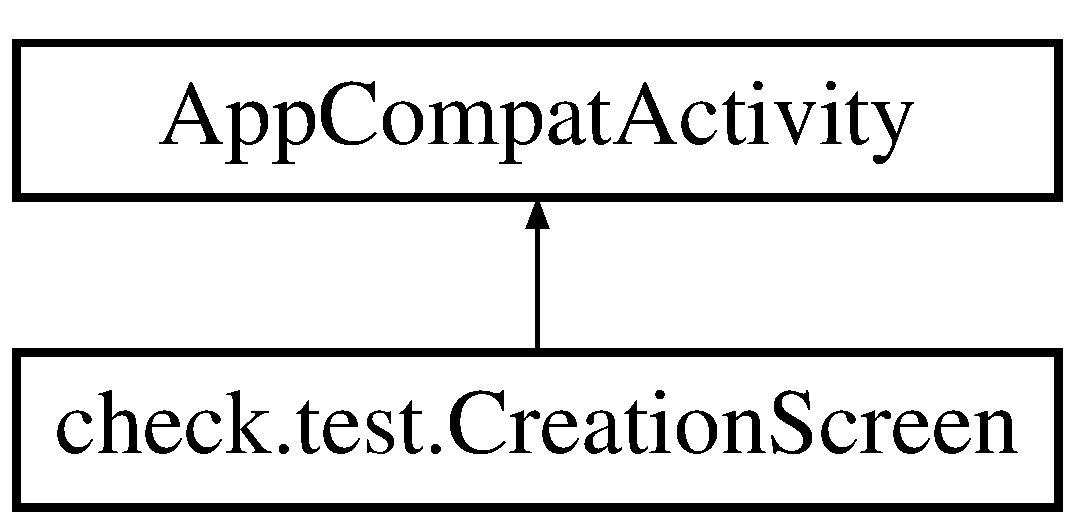
\includegraphics[height=2.000000cm]{classcheck_1_1test_1_1_creation_screen}
\end{center}
\end{figure}
\subsection*{Public Member Functions}
\begin{DoxyCompactItemize}
\item 
\hypertarget{classcheck_1_1test_1_1_creation_screen_aba9d6c11115c94e7b69ccbda460b5805}{}boolean \hyperlink{classcheck_1_1test_1_1_creation_screen_aba9d6c11115c94e7b69ccbda460b5805}{on\+Create\+Options\+Menu} (Menu menu)\label{classcheck_1_1test_1_1_creation_screen_aba9d6c11115c94e7b69ccbda460b5805}

\begin{DoxyCompactList}\small\item\em Creation of Options Menu. \end{DoxyCompactList}\item 
boolean \hyperlink{classcheck_1_1test_1_1_creation_screen_ade63dee597494e9400cda11a80e81ac5}{on\+Options\+Item\+Selected} (Menu\+Item item)
\begin{DoxyCompactList}\small\item\em Buttons to Profile Page and Settings. \end{DoxyCompactList}\end{DoxyCompactItemize}
\subsection*{Protected Member Functions}
\begin{DoxyCompactItemize}
\item 
void \hyperlink{classcheck_1_1test_1_1_creation_screen_aac8b291d450be625a519564e4f4ae7b9}{on\+Create} (Bundle saved\+Instance\+State)
\end{DoxyCompactItemize}


\subsection{Detailed Description}
Main screen for various functionality. 

Contains Favorite, Weather, Add, Randomize, Upload toolbar functionality Contains Four different visual clothe section user interfaces 

\subsection{Member Function Documentation}
\hypertarget{classcheck_1_1test_1_1_creation_screen_aac8b291d450be625a519564e4f4ae7b9}{}\index{check\+::test\+::\+Creation\+Screen@{check\+::test\+::\+Creation\+Screen}!on\+Create@{on\+Create}}
\index{on\+Create@{on\+Create}!check\+::test\+::\+Creation\+Screen@{check\+::test\+::\+Creation\+Screen}}
\subsubsection[{on\+Create(\+Bundle saved\+Instance\+State)}]{\setlength{\rightskip}{0pt plus 5cm}void check.\+test.\+Creation\+Screen.\+on\+Create (
\begin{DoxyParamCaption}
\item[{Bundle}]{saved\+Instance\+State}
\end{DoxyParamCaption}
)\hspace{0.3cm}{\ttfamily [protected]}}\label{classcheck_1_1test_1_1_creation_screen_aac8b291d450be625a519564e4f4ae7b9}
Button to saved Top clothing array

Button to saved Accessory array

Button to saved Legging clothing array

Button to saved Shoe array

Button to \hyperlink{classcheck_1_1test_1_1_favorites}{Favorites} Class

Button to Weather Class

Button to Add Class

Button to Randomize Class

Button to Upload Class \hypertarget{classcheck_1_1test_1_1_creation_screen_ade63dee597494e9400cda11a80e81ac5}{}\index{check\+::test\+::\+Creation\+Screen@{check\+::test\+::\+Creation\+Screen}!on\+Options\+Item\+Selected@{on\+Options\+Item\+Selected}}
\index{on\+Options\+Item\+Selected@{on\+Options\+Item\+Selected}!check\+::test\+::\+Creation\+Screen@{check\+::test\+::\+Creation\+Screen}}
\subsubsection[{on\+Options\+Item\+Selected(\+Menu\+Item item)}]{\setlength{\rightskip}{0pt plus 5cm}boolean check.\+test.\+Creation\+Screen.\+on\+Options\+Item\+Selected (
\begin{DoxyParamCaption}
\item[{Menu\+Item}]{item}
\end{DoxyParamCaption}
)}\label{classcheck_1_1test_1_1_creation_screen_ade63dee597494e9400cda11a80e81ac5}


Buttons to Profile Page and Settings. 

noinspection Simplifiable\+If\+Statement 

The documentation for this class was generated from the following file\+:\begin{DoxyCompactItemize}
\item 
C\+:/\+Users/\+Zwretched/.\+Android\+Studio1.\+4/\+Projects/\+Dress\+Me\+\_\+\+Android/\+Dress\+Me/src/main/java/check/test/Creation\+Screen.\+java\end{DoxyCompactItemize}

\hypertarget{classandroid_1_1support_1_1design_1_1_r_1_1dimen}{}\section{android.\+support.\+design.\+R.\+dimen Class Reference}
\label{classandroid_1_1support_1_1design_1_1_r_1_1dimen}\index{android.\+support.\+design.\+R.\+dimen@{android.\+support.\+design.\+R.\+dimen}}
\subsection*{Static Public Attributes}
\begin{DoxyCompactItemize}
\item 
\hypertarget{classandroid_1_1support_1_1design_1_1_r_1_1dimen_af42ca9b71c928b25b27c7037a575693b}{}static final int {\bfseries abc\+\_\+action\+\_\+bar\+\_\+content\+\_\+inset\+\_\+material} = 0x7f07000b\label{classandroid_1_1support_1_1design_1_1_r_1_1dimen_af42ca9b71c928b25b27c7037a575693b}

\item 
\hypertarget{classandroid_1_1support_1_1design_1_1_r_1_1dimen_ab992b60379bc68bf6d348760955ad8a6}{}static final int {\bfseries abc\+\_\+action\+\_\+bar\+\_\+default\+\_\+height\+\_\+material} = 0x7f070001\label{classandroid_1_1support_1_1design_1_1_r_1_1dimen_ab992b60379bc68bf6d348760955ad8a6}

\item 
\hypertarget{classandroid_1_1support_1_1design_1_1_r_1_1dimen_a25e4e04e667bdfbbf4bcdbced1b7d1b4}{}static final int {\bfseries abc\+\_\+action\+\_\+bar\+\_\+default\+\_\+padding\+\_\+end\+\_\+material} = 0x7f07000c\label{classandroid_1_1support_1_1design_1_1_r_1_1dimen_a25e4e04e667bdfbbf4bcdbced1b7d1b4}

\item 
\hypertarget{classandroid_1_1support_1_1design_1_1_r_1_1dimen_a0a52034a97ad09c75057adcb3a6022b1}{}static final int {\bfseries abc\+\_\+action\+\_\+bar\+\_\+default\+\_\+padding\+\_\+start\+\_\+material} = 0x7f07000d\label{classandroid_1_1support_1_1design_1_1_r_1_1dimen_a0a52034a97ad09c75057adcb3a6022b1}

\item 
\hypertarget{classandroid_1_1support_1_1design_1_1_r_1_1dimen_a45c3c747b19ec74e55fa8033393d1ac8}{}static final int {\bfseries abc\+\_\+action\+\_\+bar\+\_\+icon\+\_\+vertical\+\_\+padding\+\_\+material} = 0x7f070018\label{classandroid_1_1support_1_1design_1_1_r_1_1dimen_a45c3c747b19ec74e55fa8033393d1ac8}

\item 
\hypertarget{classandroid_1_1support_1_1design_1_1_r_1_1dimen_a953114168a0144f2305101244e1eb4bd}{}static final int {\bfseries abc\+\_\+action\+\_\+bar\+\_\+overflow\+\_\+padding\+\_\+end\+\_\+material} = 0x7f070019\label{classandroid_1_1support_1_1design_1_1_r_1_1dimen_a953114168a0144f2305101244e1eb4bd}

\item 
\hypertarget{classandroid_1_1support_1_1design_1_1_r_1_1dimen_afcc656fd9ff7526cf3a9713155929f19}{}static final int {\bfseries abc\+\_\+action\+\_\+bar\+\_\+overflow\+\_\+padding\+\_\+start\+\_\+material} = 0x7f07001a\label{classandroid_1_1support_1_1design_1_1_r_1_1dimen_afcc656fd9ff7526cf3a9713155929f19}

\item 
\hypertarget{classandroid_1_1support_1_1design_1_1_r_1_1dimen_a0841a2247b3ff85cbcaeda6ea97c0944}{}static final int {\bfseries abc\+\_\+action\+\_\+bar\+\_\+progress\+\_\+bar\+\_\+size} = 0x7f070002\label{classandroid_1_1support_1_1design_1_1_r_1_1dimen_a0841a2247b3ff85cbcaeda6ea97c0944}

\item 
\hypertarget{classandroid_1_1support_1_1design_1_1_r_1_1dimen_ab0160db7b64c23fb4ca25a6506556408}{}static final int {\bfseries abc\+\_\+action\+\_\+bar\+\_\+stacked\+\_\+max\+\_\+height} = 0x7f07001b\label{classandroid_1_1support_1_1design_1_1_r_1_1dimen_ab0160db7b64c23fb4ca25a6506556408}

\item 
\hypertarget{classandroid_1_1support_1_1design_1_1_r_1_1dimen_a8dc041a733fe2e1bb35f5791f118b1e8}{}static final int {\bfseries abc\+\_\+action\+\_\+bar\+\_\+stacked\+\_\+tab\+\_\+max\+\_\+width} = 0x7f07001c\label{classandroid_1_1support_1_1design_1_1_r_1_1dimen_a8dc041a733fe2e1bb35f5791f118b1e8}

\item 
\hypertarget{classandroid_1_1support_1_1design_1_1_r_1_1dimen_aec33706c986e5fc925371f6eb778339c}{}static final int {\bfseries abc\+\_\+action\+\_\+bar\+\_\+subtitle\+\_\+bottom\+\_\+margin\+\_\+material} = 0x7f07001d\label{classandroid_1_1support_1_1design_1_1_r_1_1dimen_aec33706c986e5fc925371f6eb778339c}

\item 
\hypertarget{classandroid_1_1support_1_1design_1_1_r_1_1dimen_ab044319f6a390e09597b7a26ca4239fa}{}static final int {\bfseries abc\+\_\+action\+\_\+bar\+\_\+subtitle\+\_\+top\+\_\+margin\+\_\+material} = 0x7f07001e\label{classandroid_1_1support_1_1design_1_1_r_1_1dimen_ab044319f6a390e09597b7a26ca4239fa}

\item 
\hypertarget{classandroid_1_1support_1_1design_1_1_r_1_1dimen_a790b0f15fe5f2eacfa6e795235d9eae4}{}static final int {\bfseries abc\+\_\+action\+\_\+button\+\_\+min\+\_\+height\+\_\+material} = 0x7f07001f\label{classandroid_1_1support_1_1design_1_1_r_1_1dimen_a790b0f15fe5f2eacfa6e795235d9eae4}

\item 
\hypertarget{classandroid_1_1support_1_1design_1_1_r_1_1dimen_a37b1e3c9da74daa257a3a466f77f4af9}{}static final int {\bfseries abc\+\_\+action\+\_\+button\+\_\+min\+\_\+width\+\_\+material} = 0x7f070020\label{classandroid_1_1support_1_1design_1_1_r_1_1dimen_a37b1e3c9da74daa257a3a466f77f4af9}

\item 
\hypertarget{classandroid_1_1support_1_1design_1_1_r_1_1dimen_a44e1469815c3f215f8034a6ad69175e4}{}static final int {\bfseries abc\+\_\+action\+\_\+button\+\_\+min\+\_\+width\+\_\+overflow\+\_\+material} = 0x7f070021\label{classandroid_1_1support_1_1design_1_1_r_1_1dimen_a44e1469815c3f215f8034a6ad69175e4}

\item 
\hypertarget{classandroid_1_1support_1_1design_1_1_r_1_1dimen_a0ac12e6518fb27a21c807a9803d7d350}{}static final int {\bfseries abc\+\_\+alert\+\_\+dialog\+\_\+button\+\_\+bar\+\_\+height} = 0x7f070000\label{classandroid_1_1support_1_1design_1_1_r_1_1dimen_a0ac12e6518fb27a21c807a9803d7d350}

\item 
\hypertarget{classandroid_1_1support_1_1design_1_1_r_1_1dimen_aa874e9a2211b7eaf3a6c6b45423ee3d5}{}static final int {\bfseries abc\+\_\+button\+\_\+inset\+\_\+horizontal\+\_\+material} = 0x7f070022\label{classandroid_1_1support_1_1design_1_1_r_1_1dimen_aa874e9a2211b7eaf3a6c6b45423ee3d5}

\item 
\hypertarget{classandroid_1_1support_1_1design_1_1_r_1_1dimen_a4f55256e84d9d47f13cf1553adbbb153}{}static final int {\bfseries abc\+\_\+button\+\_\+inset\+\_\+vertical\+\_\+material} = 0x7f070023\label{classandroid_1_1support_1_1design_1_1_r_1_1dimen_a4f55256e84d9d47f13cf1553adbbb153}

\item 
\hypertarget{classandroid_1_1support_1_1design_1_1_r_1_1dimen_adf85bcb0e234cbc7883e6d6e6dc005e3}{}static final int {\bfseries abc\+\_\+button\+\_\+padding\+\_\+horizontal\+\_\+material} = 0x7f070024\label{classandroid_1_1support_1_1design_1_1_r_1_1dimen_adf85bcb0e234cbc7883e6d6e6dc005e3}

\item 
\hypertarget{classandroid_1_1support_1_1design_1_1_r_1_1dimen_a15726a35ff8b417641bbc00e360df277}{}static final int {\bfseries abc\+\_\+button\+\_\+padding\+\_\+vertical\+\_\+material} = 0x7f070025\label{classandroid_1_1support_1_1design_1_1_r_1_1dimen_a15726a35ff8b417641bbc00e360df277}

\item 
\hypertarget{classandroid_1_1support_1_1design_1_1_r_1_1dimen_ada9bce90209861ef96ac780cc525730c}{}static final int {\bfseries abc\+\_\+config\+\_\+pref\+Dialog\+Width} = 0x7f070005\label{classandroid_1_1support_1_1design_1_1_r_1_1dimen_ada9bce90209861ef96ac780cc525730c}

\item 
\hypertarget{classandroid_1_1support_1_1design_1_1_r_1_1dimen_a309e3353e64253f83debdb45d1449e74}{}static final int {\bfseries abc\+\_\+control\+\_\+corner\+\_\+material} = 0x7f070026\label{classandroid_1_1support_1_1design_1_1_r_1_1dimen_a309e3353e64253f83debdb45d1449e74}

\item 
\hypertarget{classandroid_1_1support_1_1design_1_1_r_1_1dimen_a2be8e6d98d31e9f2a87de1071f804927}{}static final int {\bfseries abc\+\_\+control\+\_\+inset\+\_\+material} = 0x7f070027\label{classandroid_1_1support_1_1design_1_1_r_1_1dimen_a2be8e6d98d31e9f2a87de1071f804927}

\item 
\hypertarget{classandroid_1_1support_1_1design_1_1_r_1_1dimen_a8019524092bba937679a2feb43ed2dc0}{}static final int {\bfseries abc\+\_\+control\+\_\+padding\+\_\+material} = 0x7f070028\label{classandroid_1_1support_1_1design_1_1_r_1_1dimen_a8019524092bba937679a2feb43ed2dc0}

\item 
\hypertarget{classandroid_1_1support_1_1design_1_1_r_1_1dimen_a21d5b070cecbc9e8604e17ca90292be4}{}static final int {\bfseries abc\+\_\+dialog\+\_\+list\+\_\+padding\+\_\+vertical\+\_\+material} = 0x7f070029\label{classandroid_1_1support_1_1design_1_1_r_1_1dimen_a21d5b070cecbc9e8604e17ca90292be4}

\item 
\hypertarget{classandroid_1_1support_1_1design_1_1_r_1_1dimen_a15f18eb1f09e97f0916635c3b780e3d4}{}static final int {\bfseries abc\+\_\+dialog\+\_\+min\+\_\+width\+\_\+major} = 0x7f07002a\label{classandroid_1_1support_1_1design_1_1_r_1_1dimen_a15f18eb1f09e97f0916635c3b780e3d4}

\item 
\hypertarget{classandroid_1_1support_1_1design_1_1_r_1_1dimen_a6a73848d8d821f2d6fcf111851f69708}{}static final int {\bfseries abc\+\_\+dialog\+\_\+min\+\_\+width\+\_\+minor} = 0x7f07002b\label{classandroid_1_1support_1_1design_1_1_r_1_1dimen_a6a73848d8d821f2d6fcf111851f69708}

\item 
\hypertarget{classandroid_1_1support_1_1design_1_1_r_1_1dimen_a520740e21ad1d52830d8977ff10afd5e}{}static final int {\bfseries abc\+\_\+dialog\+\_\+padding\+\_\+material} = 0x7f07002c\label{classandroid_1_1support_1_1design_1_1_r_1_1dimen_a520740e21ad1d52830d8977ff10afd5e}

\item 
\hypertarget{classandroid_1_1support_1_1design_1_1_r_1_1dimen_affd502ad3ee057bb26d6ce1cd4cc89b6}{}static final int {\bfseries abc\+\_\+dialog\+\_\+padding\+\_\+top\+\_\+material} = 0x7f07002d\label{classandroid_1_1support_1_1design_1_1_r_1_1dimen_affd502ad3ee057bb26d6ce1cd4cc89b6}

\item 
\hypertarget{classandroid_1_1support_1_1design_1_1_r_1_1dimen_a711065db6123eeca1bdda1feae6ee604}{}static final int {\bfseries abc\+\_\+disabled\+\_\+alpha\+\_\+material\+\_\+dark} = 0x7f07002e\label{classandroid_1_1support_1_1design_1_1_r_1_1dimen_a711065db6123eeca1bdda1feae6ee604}

\item 
\hypertarget{classandroid_1_1support_1_1design_1_1_r_1_1dimen_ad1756a425760ec484cfb76295400d4db}{}static final int {\bfseries abc\+\_\+disabled\+\_\+alpha\+\_\+material\+\_\+light} = 0x7f07002f\label{classandroid_1_1support_1_1design_1_1_r_1_1dimen_ad1756a425760ec484cfb76295400d4db}

\item 
\hypertarget{classandroid_1_1support_1_1design_1_1_r_1_1dimen_acc8d9f0a4c9277aa49a4c1cc8090c70e}{}static final int {\bfseries abc\+\_\+dropdownitem\+\_\+icon\+\_\+width} = 0x7f070030\label{classandroid_1_1support_1_1design_1_1_r_1_1dimen_acc8d9f0a4c9277aa49a4c1cc8090c70e}

\item 
\hypertarget{classandroid_1_1support_1_1design_1_1_r_1_1dimen_a968fc63b6429432c490e18cf8e1ae698}{}static final int {\bfseries abc\+\_\+dropdownitem\+\_\+text\+\_\+padding\+\_\+left} = 0x7f070031\label{classandroid_1_1support_1_1design_1_1_r_1_1dimen_a968fc63b6429432c490e18cf8e1ae698}

\item 
\hypertarget{classandroid_1_1support_1_1design_1_1_r_1_1dimen_aeec29d97219b2c603cdeb98e26965a7a}{}static final int {\bfseries abc\+\_\+dropdownitem\+\_\+text\+\_\+padding\+\_\+right} = 0x7f070032\label{classandroid_1_1support_1_1design_1_1_r_1_1dimen_aeec29d97219b2c603cdeb98e26965a7a}

\item 
\hypertarget{classandroid_1_1support_1_1design_1_1_r_1_1dimen_a0985e21f84e746dec037773a3abb1113}{}static final int {\bfseries abc\+\_\+edit\+\_\+text\+\_\+inset\+\_\+bottom\+\_\+material} = 0x7f070033\label{classandroid_1_1support_1_1design_1_1_r_1_1dimen_a0985e21f84e746dec037773a3abb1113}

\item 
\hypertarget{classandroid_1_1support_1_1design_1_1_r_1_1dimen_aedd7d9d99b8c4f081a9582ae33e056c4}{}static final int {\bfseries abc\+\_\+edit\+\_\+text\+\_\+inset\+\_\+horizontal\+\_\+material} = 0x7f070034\label{classandroid_1_1support_1_1design_1_1_r_1_1dimen_aedd7d9d99b8c4f081a9582ae33e056c4}

\item 
\hypertarget{classandroid_1_1support_1_1design_1_1_r_1_1dimen_ac9ec7c237aed1411b8bf85d1f2de801b}{}static final int {\bfseries abc\+\_\+edit\+\_\+text\+\_\+inset\+\_\+top\+\_\+material} = 0x7f070035\label{classandroid_1_1support_1_1design_1_1_r_1_1dimen_ac9ec7c237aed1411b8bf85d1f2de801b}

\item 
\hypertarget{classandroid_1_1support_1_1design_1_1_r_1_1dimen_a7c730cc453da03509011d0f75524689a}{}static final int {\bfseries abc\+\_\+floating\+\_\+window\+\_\+z} = 0x7f070036\label{classandroid_1_1support_1_1design_1_1_r_1_1dimen_a7c730cc453da03509011d0f75524689a}

\item 
\hypertarget{classandroid_1_1support_1_1design_1_1_r_1_1dimen_a2876e7547b2e4660135953655f79ff25}{}static final int {\bfseries abc\+\_\+list\+\_\+item\+\_\+padding\+\_\+horizontal\+\_\+material} = 0x7f070037\label{classandroid_1_1support_1_1design_1_1_r_1_1dimen_a2876e7547b2e4660135953655f79ff25}

\item 
\hypertarget{classandroid_1_1support_1_1design_1_1_r_1_1dimen_a365e3bc959933ee12d8b935ea42253de}{}static final int {\bfseries abc\+\_\+panel\+\_\+menu\+\_\+list\+\_\+width} = 0x7f070038\label{classandroid_1_1support_1_1design_1_1_r_1_1dimen_a365e3bc959933ee12d8b935ea42253de}

\item 
\hypertarget{classandroid_1_1support_1_1design_1_1_r_1_1dimen_a6901ca34b7cc25c725a55d9973e6c0c5}{}static final int {\bfseries abc\+\_\+search\+\_\+view\+\_\+preferred\+\_\+width} = 0x7f070039\label{classandroid_1_1support_1_1design_1_1_r_1_1dimen_a6901ca34b7cc25c725a55d9973e6c0c5}

\item 
\hypertarget{classandroid_1_1support_1_1design_1_1_r_1_1dimen_a986b8c7dc11c0933e28f3f72ed50578e}{}static final int {\bfseries abc\+\_\+search\+\_\+view\+\_\+text\+\_\+min\+\_\+width} = 0x7f070006\label{classandroid_1_1support_1_1design_1_1_r_1_1dimen_a986b8c7dc11c0933e28f3f72ed50578e}

\item 
\hypertarget{classandroid_1_1support_1_1design_1_1_r_1_1dimen_a68dfff3b44493d46ef4f342fe493b6f1}{}static final int {\bfseries abc\+\_\+switch\+\_\+padding} = 0x7f070015\label{classandroid_1_1support_1_1design_1_1_r_1_1dimen_a68dfff3b44493d46ef4f342fe493b6f1}

\item 
\hypertarget{classandroid_1_1support_1_1design_1_1_r_1_1dimen_ab0b6acfb59c02b2774843fb880ffcf8a}{}static final int {\bfseries abc\+\_\+text\+\_\+size\+\_\+body\+\_\+1\+\_\+material} = 0x7f07003a\label{classandroid_1_1support_1_1design_1_1_r_1_1dimen_ab0b6acfb59c02b2774843fb880ffcf8a}

\item 
\hypertarget{classandroid_1_1support_1_1design_1_1_r_1_1dimen_a528fe8a33f9ff3e67b652f558ee25c2d}{}static final int {\bfseries abc\+\_\+text\+\_\+size\+\_\+body\+\_\+2\+\_\+material} = 0x7f07003b\label{classandroid_1_1support_1_1design_1_1_r_1_1dimen_a528fe8a33f9ff3e67b652f558ee25c2d}

\item 
\hypertarget{classandroid_1_1support_1_1design_1_1_r_1_1dimen_a88aed06e5c28e04e97f8b700b4e51593}{}static final int {\bfseries abc\+\_\+text\+\_\+size\+\_\+button\+\_\+material} = 0x7f07003c\label{classandroid_1_1support_1_1design_1_1_r_1_1dimen_a88aed06e5c28e04e97f8b700b4e51593}

\item 
\hypertarget{classandroid_1_1support_1_1design_1_1_r_1_1dimen_a5cdfadc5f166849cf34b222d8d3f684e}{}static final int {\bfseries abc\+\_\+text\+\_\+size\+\_\+caption\+\_\+material} = 0x7f07003d\label{classandroid_1_1support_1_1design_1_1_r_1_1dimen_a5cdfadc5f166849cf34b222d8d3f684e}

\item 
\hypertarget{classandroid_1_1support_1_1design_1_1_r_1_1dimen_a691b8577be670e47f62cc11833ca1e7b}{}static final int {\bfseries abc\+\_\+text\+\_\+size\+\_\+display\+\_\+1\+\_\+material} = 0x7f07003e\label{classandroid_1_1support_1_1design_1_1_r_1_1dimen_a691b8577be670e47f62cc11833ca1e7b}

\item 
\hypertarget{classandroid_1_1support_1_1design_1_1_r_1_1dimen_aa795c05c797d5e84e8e16eae582c74e0}{}static final int {\bfseries abc\+\_\+text\+\_\+size\+\_\+display\+\_\+2\+\_\+material} = 0x7f07003f\label{classandroid_1_1support_1_1design_1_1_r_1_1dimen_aa795c05c797d5e84e8e16eae582c74e0}

\item 
\hypertarget{classandroid_1_1support_1_1design_1_1_r_1_1dimen_af16a183a043f3ce464a8daec9e04da9a}{}static final int {\bfseries abc\+\_\+text\+\_\+size\+\_\+display\+\_\+3\+\_\+material} = 0x7f070040\label{classandroid_1_1support_1_1design_1_1_r_1_1dimen_af16a183a043f3ce464a8daec9e04da9a}

\item 
\hypertarget{classandroid_1_1support_1_1design_1_1_r_1_1dimen_a8e55855f262f4e761dd55609d351e8af}{}static final int {\bfseries abc\+\_\+text\+\_\+size\+\_\+display\+\_\+4\+\_\+material} = 0x7f070041\label{classandroid_1_1support_1_1design_1_1_r_1_1dimen_a8e55855f262f4e761dd55609d351e8af}

\item 
\hypertarget{classandroid_1_1support_1_1design_1_1_r_1_1dimen_a2081000949435fecb9964aa41ab05907}{}static final int {\bfseries abc\+\_\+text\+\_\+size\+\_\+headline\+\_\+material} = 0x7f070042\label{classandroid_1_1support_1_1design_1_1_r_1_1dimen_a2081000949435fecb9964aa41ab05907}

\item 
\hypertarget{classandroid_1_1support_1_1design_1_1_r_1_1dimen_af1d4e99b6a3ce4f2fb3ba72c6b953412}{}static final int {\bfseries abc\+\_\+text\+\_\+size\+\_\+large\+\_\+material} = 0x7f070043\label{classandroid_1_1support_1_1design_1_1_r_1_1dimen_af1d4e99b6a3ce4f2fb3ba72c6b953412}

\item 
\hypertarget{classandroid_1_1support_1_1design_1_1_r_1_1dimen_a6479afaabebd9416c3403c54b0f5bd59}{}static final int {\bfseries abc\+\_\+text\+\_\+size\+\_\+medium\+\_\+material} = 0x7f070044\label{classandroid_1_1support_1_1design_1_1_r_1_1dimen_a6479afaabebd9416c3403c54b0f5bd59}

\item 
\hypertarget{classandroid_1_1support_1_1design_1_1_r_1_1dimen_a03965514ad78473ff07b5eba8191081b}{}static final int {\bfseries abc\+\_\+text\+\_\+size\+\_\+menu\+\_\+material} = 0x7f070045\label{classandroid_1_1support_1_1design_1_1_r_1_1dimen_a03965514ad78473ff07b5eba8191081b}

\item 
\hypertarget{classandroid_1_1support_1_1design_1_1_r_1_1dimen_a8a4fb3e596b4b3a400c7623b71bf5ff3}{}static final int {\bfseries abc\+\_\+text\+\_\+size\+\_\+small\+\_\+material} = 0x7f070046\label{classandroid_1_1support_1_1design_1_1_r_1_1dimen_a8a4fb3e596b4b3a400c7623b71bf5ff3}

\item 
\hypertarget{classandroid_1_1support_1_1design_1_1_r_1_1dimen_aebb837455075fb116b55f1e630d32dd5}{}static final int {\bfseries abc\+\_\+text\+\_\+size\+\_\+subhead\+\_\+material} = 0x7f070047\label{classandroid_1_1support_1_1design_1_1_r_1_1dimen_aebb837455075fb116b55f1e630d32dd5}

\item 
\hypertarget{classandroid_1_1support_1_1design_1_1_r_1_1dimen_a2c3b879fdd2573d992fedf97f0e2295b}{}static final int {\bfseries abc\+\_\+text\+\_\+size\+\_\+subtitle\+\_\+material\+\_\+toolbar} = 0x7f070003\label{classandroid_1_1support_1_1design_1_1_r_1_1dimen_a2c3b879fdd2573d992fedf97f0e2295b}

\item 
\hypertarget{classandroid_1_1support_1_1design_1_1_r_1_1dimen_abbfc491717374b99ef03c57688c58ec0}{}static final int {\bfseries abc\+\_\+text\+\_\+size\+\_\+title\+\_\+material} = 0x7f070048\label{classandroid_1_1support_1_1design_1_1_r_1_1dimen_abbfc491717374b99ef03c57688c58ec0}

\item 
\hypertarget{classandroid_1_1support_1_1design_1_1_r_1_1dimen_a7f3928a1b96bdd9950713ed0212b419a}{}static final int {\bfseries abc\+\_\+text\+\_\+size\+\_\+title\+\_\+material\+\_\+toolbar} = 0x7f070004\label{classandroid_1_1support_1_1design_1_1_r_1_1dimen_a7f3928a1b96bdd9950713ed0212b419a}

\item 
\hypertarget{classandroid_1_1support_1_1design_1_1_r_1_1dimen_ad02702f8e442d5ce2161992d960183a4}{}static final int {\bfseries design\+\_\+appbar\+\_\+elevation} = 0x7f07004a\label{classandroid_1_1support_1_1design_1_1_r_1_1dimen_ad02702f8e442d5ce2161992d960183a4}

\item 
\hypertarget{classandroid_1_1support_1_1design_1_1_r_1_1dimen_af4f3a9ee873d7757d2dd0be1c2cadf4b}{}static final int {\bfseries design\+\_\+fab\+\_\+border\+\_\+width} = 0x7f07004b\label{classandroid_1_1support_1_1design_1_1_r_1_1dimen_af4f3a9ee873d7757d2dd0be1c2cadf4b}

\item 
\hypertarget{classandroid_1_1support_1_1design_1_1_r_1_1dimen_a640034d9a7862b244c921bc9d8d01889}{}static final int {\bfseries design\+\_\+fab\+\_\+content\+\_\+size} = 0x7f07004c\label{classandroid_1_1support_1_1design_1_1_r_1_1dimen_a640034d9a7862b244c921bc9d8d01889}

\item 
\hypertarget{classandroid_1_1support_1_1design_1_1_r_1_1dimen_a6fe7a893bf5c66341ebde39a58bdcf97}{}static final int {\bfseries design\+\_\+fab\+\_\+elevation} = 0x7f07004d\label{classandroid_1_1support_1_1design_1_1_r_1_1dimen_a6fe7a893bf5c66341ebde39a58bdcf97}

\item 
\hypertarget{classandroid_1_1support_1_1design_1_1_r_1_1dimen_ad2f1e3630649a6bf663595a91a73bb75}{}static final int {\bfseries design\+\_\+fab\+\_\+size\+\_\+mini} = 0x7f07004e\label{classandroid_1_1support_1_1design_1_1_r_1_1dimen_ad2f1e3630649a6bf663595a91a73bb75}

\item 
\hypertarget{classandroid_1_1support_1_1design_1_1_r_1_1dimen_a1149e0b937576ec45f347e32bd7c0995}{}static final int {\bfseries design\+\_\+fab\+\_\+size\+\_\+normal} = 0x7f07004f\label{classandroid_1_1support_1_1design_1_1_r_1_1dimen_a1149e0b937576ec45f347e32bd7c0995}

\item 
\hypertarget{classandroid_1_1support_1_1design_1_1_r_1_1dimen_a51c58f3bb12ba528b250d93588890122}{}static final int {\bfseries design\+\_\+fab\+\_\+translation\+\_\+z\+\_\+pressed} = 0x7f070050\label{classandroid_1_1support_1_1design_1_1_r_1_1dimen_a51c58f3bb12ba528b250d93588890122}

\item 
\hypertarget{classandroid_1_1support_1_1design_1_1_r_1_1dimen_aefa62bedc2505b09d491e969011487c7}{}static final int {\bfseries design\+\_\+navigation\+\_\+elevation} = 0x7f070051\label{classandroid_1_1support_1_1design_1_1_r_1_1dimen_aefa62bedc2505b09d491e969011487c7}

\item 
\hypertarget{classandroid_1_1support_1_1design_1_1_r_1_1dimen_ae84d41ce904136aaafbbd73e8d23ed55}{}static final int {\bfseries design\+\_\+navigation\+\_\+icon\+\_\+padding} = 0x7f070052\label{classandroid_1_1support_1_1design_1_1_r_1_1dimen_ae84d41ce904136aaafbbd73e8d23ed55}

\item 
\hypertarget{classandroid_1_1support_1_1design_1_1_r_1_1dimen_a09a0e74d4044391a347f715900c8ba05}{}static final int {\bfseries design\+\_\+navigation\+\_\+icon\+\_\+size} = 0x7f070053\label{classandroid_1_1support_1_1design_1_1_r_1_1dimen_a09a0e74d4044391a347f715900c8ba05}

\item 
\hypertarget{classandroid_1_1support_1_1design_1_1_r_1_1dimen_aea61310378807a0bf7cf2f2a8a494681}{}static final int {\bfseries design\+\_\+navigation\+\_\+max\+\_\+width} = 0x7f070054\label{classandroid_1_1support_1_1design_1_1_r_1_1dimen_aea61310378807a0bf7cf2f2a8a494681}

\item 
\hypertarget{classandroid_1_1support_1_1design_1_1_r_1_1dimen_a2647e9da0be00a73db532944c5288a3a}{}static final int {\bfseries design\+\_\+navigation\+\_\+padding\+\_\+bottom} = 0x7f070055\label{classandroid_1_1support_1_1design_1_1_r_1_1dimen_a2647e9da0be00a73db532944c5288a3a}

\item 
\hypertarget{classandroid_1_1support_1_1design_1_1_r_1_1dimen_a70d368b727ec0c602d584cc5b8a8364d}{}static final int {\bfseries design\+\_\+navigation\+\_\+padding\+\_\+top\+\_\+default} = 0x7f070016\label{classandroid_1_1support_1_1design_1_1_r_1_1dimen_a70d368b727ec0c602d584cc5b8a8364d}

\item 
\hypertarget{classandroid_1_1support_1_1design_1_1_r_1_1dimen_ad6a3bb1231788391e52c4896d0de39f7}{}static final int {\bfseries design\+\_\+navigation\+\_\+separator\+\_\+vertical\+\_\+padding} = 0x7f070056\label{classandroid_1_1support_1_1design_1_1_r_1_1dimen_ad6a3bb1231788391e52c4896d0de39f7}

\item 
\hypertarget{classandroid_1_1support_1_1design_1_1_r_1_1dimen_a6ec8da0fd7402fc33d6180aff7258f88}{}static final int {\bfseries design\+\_\+snackbar\+\_\+action\+\_\+inline\+\_\+max\+\_\+width} = 0x7f07000e\label{classandroid_1_1support_1_1design_1_1_r_1_1dimen_a6ec8da0fd7402fc33d6180aff7258f88}

\item 
\hypertarget{classandroid_1_1support_1_1design_1_1_r_1_1dimen_a469c963201807723e61ebd63d9d31b30}{}static final int {\bfseries design\+\_\+snackbar\+\_\+background\+\_\+corner\+\_\+radius} = 0x7f07000f\label{classandroid_1_1support_1_1design_1_1_r_1_1dimen_a469c963201807723e61ebd63d9d31b30}

\item 
\hypertarget{classandroid_1_1support_1_1design_1_1_r_1_1dimen_a618410f7930e7304fc24480e003f2f48}{}static final int {\bfseries design\+\_\+snackbar\+\_\+elevation} = 0x7f070057\label{classandroid_1_1support_1_1design_1_1_r_1_1dimen_a618410f7930e7304fc24480e003f2f48}

\item 
\hypertarget{classandroid_1_1support_1_1design_1_1_r_1_1dimen_a9d7da239527c985b37edc815e1f67bd8}{}static final int {\bfseries design\+\_\+snackbar\+\_\+extra\+\_\+spacing\+\_\+horizontal} = 0x7f070010\label{classandroid_1_1support_1_1design_1_1_r_1_1dimen_a9d7da239527c985b37edc815e1f67bd8}

\item 
\hypertarget{classandroid_1_1support_1_1design_1_1_r_1_1dimen_ae088decd1622475be59b157ddd788bb6}{}static final int {\bfseries design\+\_\+snackbar\+\_\+max\+\_\+width} = 0x7f070011\label{classandroid_1_1support_1_1design_1_1_r_1_1dimen_ae088decd1622475be59b157ddd788bb6}

\item 
\hypertarget{classandroid_1_1support_1_1design_1_1_r_1_1dimen_ad801c273260b6b31c3f8b25b24888e31}{}static final int {\bfseries design\+\_\+snackbar\+\_\+min\+\_\+width} = 0x7f070012\label{classandroid_1_1support_1_1design_1_1_r_1_1dimen_ad801c273260b6b31c3f8b25b24888e31}

\item 
\hypertarget{classandroid_1_1support_1_1design_1_1_r_1_1dimen_a009e67819dc08e09556179677e7d7209}{}static final int {\bfseries design\+\_\+snackbar\+\_\+padding\+\_\+horizontal} = 0x7f070058\label{classandroid_1_1support_1_1design_1_1_r_1_1dimen_a009e67819dc08e09556179677e7d7209}

\item 
\hypertarget{classandroid_1_1support_1_1design_1_1_r_1_1dimen_a7fac1342910fbb66edd76b36ffb0040c}{}static final int {\bfseries design\+\_\+snackbar\+\_\+padding\+\_\+vertical} = 0x7f070059\label{classandroid_1_1support_1_1design_1_1_r_1_1dimen_a7fac1342910fbb66edd76b36ffb0040c}

\item 
\hypertarget{classandroid_1_1support_1_1design_1_1_r_1_1dimen_a763a99a7ed4d51adad516e2789989919}{}static final int {\bfseries design\+\_\+snackbar\+\_\+padding\+\_\+vertical\+\_\+2lines} = 0x7f070013\label{classandroid_1_1support_1_1design_1_1_r_1_1dimen_a763a99a7ed4d51adad516e2789989919}

\item 
\hypertarget{classandroid_1_1support_1_1design_1_1_r_1_1dimen_a52aa6de59674be234038a285bd18813e}{}static final int {\bfseries design\+\_\+snackbar\+\_\+text\+\_\+size} = 0x7f07005a\label{classandroid_1_1support_1_1design_1_1_r_1_1dimen_a52aa6de59674be234038a285bd18813e}

\item 
\hypertarget{classandroid_1_1support_1_1design_1_1_r_1_1dimen_a5b6cc64ba88e605a0388ebbfe495d251}{}static final int {\bfseries design\+\_\+tab\+\_\+max\+\_\+width} = 0x7f07005b\label{classandroid_1_1support_1_1design_1_1_r_1_1dimen_a5b6cc64ba88e605a0388ebbfe495d251}

\item 
\hypertarget{classandroid_1_1support_1_1design_1_1_r_1_1dimen_a2684f1df7b43f3c950f74c4de9aee2cb}{}static final int {\bfseries design\+\_\+tab\+\_\+min\+\_\+width} = 0x7f070014\label{classandroid_1_1support_1_1design_1_1_r_1_1dimen_a2684f1df7b43f3c950f74c4de9aee2cb}

\item 
\hypertarget{classandroid_1_1support_1_1design_1_1_r_1_1dimen_a7d982a70f8fe2b22a40f0ca43d0c50e6}{}static final int {\bfseries dialog\+\_\+fixed\+\_\+height\+\_\+major} = 0x7f070007\label{classandroid_1_1support_1_1design_1_1_r_1_1dimen_a7d982a70f8fe2b22a40f0ca43d0c50e6}

\item 
\hypertarget{classandroid_1_1support_1_1design_1_1_r_1_1dimen_a06e7f792a3148e50450a94ad0fe0249f}{}static final int {\bfseries dialog\+\_\+fixed\+\_\+height\+\_\+minor} = 0x7f070008\label{classandroid_1_1support_1_1design_1_1_r_1_1dimen_a06e7f792a3148e50450a94ad0fe0249f}

\item 
\hypertarget{classandroid_1_1support_1_1design_1_1_r_1_1dimen_a7de4278fd677ac5a62001924a804377c}{}static final int {\bfseries dialog\+\_\+fixed\+\_\+width\+\_\+major} = 0x7f070009\label{classandroid_1_1support_1_1design_1_1_r_1_1dimen_a7de4278fd677ac5a62001924a804377c}

\item 
\hypertarget{classandroid_1_1support_1_1design_1_1_r_1_1dimen_ab07db9c92256c3cff825b13409bfff5a}{}static final int {\bfseries dialog\+\_\+fixed\+\_\+width\+\_\+minor} = 0x7f07000a\label{classandroid_1_1support_1_1design_1_1_r_1_1dimen_ab07db9c92256c3cff825b13409bfff5a}

\item 
\hypertarget{classandroid_1_1support_1_1design_1_1_r_1_1dimen_abaf724b0a152c084b87b3a250eb9925e}{}static final int {\bfseries disabled\+\_\+alpha\+\_\+material\+\_\+dark} = 0x7f07005c\label{classandroid_1_1support_1_1design_1_1_r_1_1dimen_abaf724b0a152c084b87b3a250eb9925e}

\item 
\hypertarget{classandroid_1_1support_1_1design_1_1_r_1_1dimen_a5ff754097768daa1ae8597556ab0a5a5}{}static final int {\bfseries disabled\+\_\+alpha\+\_\+material\+\_\+light} = 0x7f07005d\label{classandroid_1_1support_1_1design_1_1_r_1_1dimen_a5ff754097768daa1ae8597556ab0a5a5}

\item 
\hypertarget{classandroid_1_1support_1_1design_1_1_r_1_1dimen_a844066f047b47ae2ef832ac7e8ece4c2}{}static final int {\bfseries highlight\+\_\+alpha\+\_\+material\+\_\+colored} = 0x7f07005f\label{classandroid_1_1support_1_1design_1_1_r_1_1dimen_a844066f047b47ae2ef832ac7e8ece4c2}

\item 
\hypertarget{classandroid_1_1support_1_1design_1_1_r_1_1dimen_ad4138b2c901c676ceb97b62ece7c5bad}{}static final int {\bfseries highlight\+\_\+alpha\+\_\+material\+\_\+dark} = 0x7f070060\label{classandroid_1_1support_1_1design_1_1_r_1_1dimen_ad4138b2c901c676ceb97b62ece7c5bad}

\item 
\hypertarget{classandroid_1_1support_1_1design_1_1_r_1_1dimen_aae4ec3504ac5846750b92f88579b6046}{}static final int {\bfseries highlight\+\_\+alpha\+\_\+material\+\_\+light} = 0x7f070061\label{classandroid_1_1support_1_1design_1_1_r_1_1dimen_aae4ec3504ac5846750b92f88579b6046}

\item 
\hypertarget{classandroid_1_1support_1_1design_1_1_r_1_1dimen_a6ad558115ac7ce4e1ce9a38b30aa6034}{}static final int {\bfseries notification\+\_\+large\+\_\+icon\+\_\+height} = 0x7f070062\label{classandroid_1_1support_1_1design_1_1_r_1_1dimen_a6ad558115ac7ce4e1ce9a38b30aa6034}

\item 
\hypertarget{classandroid_1_1support_1_1design_1_1_r_1_1dimen_acdf22e449222145bfdff5402ada49f70}{}static final int {\bfseries notification\+\_\+large\+\_\+icon\+\_\+width} = 0x7f070063\label{classandroid_1_1support_1_1design_1_1_r_1_1dimen_acdf22e449222145bfdff5402ada49f70}

\item 
\hypertarget{classandroid_1_1support_1_1design_1_1_r_1_1dimen_a971afa031fc61e3559e18f13f8d09792}{}static final int {\bfseries notification\+\_\+subtext\+\_\+size} = 0x7f070064\label{classandroid_1_1support_1_1design_1_1_r_1_1dimen_a971afa031fc61e3559e18f13f8d09792}

\end{DoxyCompactItemize}


The documentation for this class was generated from the following file\+:\begin{DoxyCompactItemize}
\item 
C\+:/\+Users/\+Zwretched/.\+Android\+Studio1.\+4/\+Projects/\+Dress\+Me\+\_\+\+Android/\+Dress\+Me/build/generated/source/r/debug/android/support/design/R.\+java\end{DoxyCompactItemize}

\hypertarget{classcheck_1_1test_1_1_r_1_1dimen}{}\section{check.\+test.\+R.\+dimen Class Reference}
\label{classcheck_1_1test_1_1_r_1_1dimen}\index{check.\+test.\+R.\+dimen@{check.\+test.\+R.\+dimen}}
\subsection*{Static Public Attributes}
\begin{DoxyCompactItemize}
\item 
\hypertarget{classcheck_1_1test_1_1_r_1_1dimen_af8791e998f4065b67a9c0017c861f5d9}{}static final int {\bfseries abc\+\_\+action\+\_\+bar\+\_\+content\+\_\+inset\+\_\+material} =0x7f07000b\label{classcheck_1_1test_1_1_r_1_1dimen_af8791e998f4065b67a9c0017c861f5d9}

\item 
\hypertarget{classcheck_1_1test_1_1_r_1_1dimen_a38ae460b19eb7368dd2fefda56cbe7ad}{}static final int {\bfseries abc\+\_\+action\+\_\+bar\+\_\+default\+\_\+height\+\_\+material} =0x7f070001\label{classcheck_1_1test_1_1_r_1_1dimen_a38ae460b19eb7368dd2fefda56cbe7ad}

\item 
\hypertarget{classcheck_1_1test_1_1_r_1_1dimen_aba5f5173544414aedb06612c16488e8a}{}static final int {\bfseries abc\+\_\+action\+\_\+bar\+\_\+default\+\_\+padding\+\_\+end\+\_\+material} =0x7f07000c\label{classcheck_1_1test_1_1_r_1_1dimen_aba5f5173544414aedb06612c16488e8a}

\item 
\hypertarget{classcheck_1_1test_1_1_r_1_1dimen_a288de3730e75f6ae54f92d2615c61d26}{}static final int {\bfseries abc\+\_\+action\+\_\+bar\+\_\+default\+\_\+padding\+\_\+start\+\_\+material} =0x7f07000d\label{classcheck_1_1test_1_1_r_1_1dimen_a288de3730e75f6ae54f92d2615c61d26}

\item 
\hypertarget{classcheck_1_1test_1_1_r_1_1dimen_a53a51402fac4702df79d782042907c3d}{}static final int {\bfseries abc\+\_\+action\+\_\+bar\+\_\+icon\+\_\+vertical\+\_\+padding\+\_\+material} =0x7f070018\label{classcheck_1_1test_1_1_r_1_1dimen_a53a51402fac4702df79d782042907c3d}

\item 
\hypertarget{classcheck_1_1test_1_1_r_1_1dimen_a6e171c9254943503176474614ed66d6e}{}static final int {\bfseries abc\+\_\+action\+\_\+bar\+\_\+overflow\+\_\+padding\+\_\+end\+\_\+material} =0x7f070019\label{classcheck_1_1test_1_1_r_1_1dimen_a6e171c9254943503176474614ed66d6e}

\item 
\hypertarget{classcheck_1_1test_1_1_r_1_1dimen_ad969da99713b581daab3061d6db8a49b}{}static final int {\bfseries abc\+\_\+action\+\_\+bar\+\_\+overflow\+\_\+padding\+\_\+start\+\_\+material} =0x7f07001a\label{classcheck_1_1test_1_1_r_1_1dimen_ad969da99713b581daab3061d6db8a49b}

\item 
\hypertarget{classcheck_1_1test_1_1_r_1_1dimen_a2d21081705d41c257d4572203da96a5a}{}static final int {\bfseries abc\+\_\+action\+\_\+bar\+\_\+progress\+\_\+bar\+\_\+size} =0x7f070002\label{classcheck_1_1test_1_1_r_1_1dimen_a2d21081705d41c257d4572203da96a5a}

\item 
\hypertarget{classcheck_1_1test_1_1_r_1_1dimen_aee9ed59153261299d47b8fa9679c329e}{}static final int {\bfseries abc\+\_\+action\+\_\+bar\+\_\+stacked\+\_\+max\+\_\+height} =0x7f07001b\label{classcheck_1_1test_1_1_r_1_1dimen_aee9ed59153261299d47b8fa9679c329e}

\item 
\hypertarget{classcheck_1_1test_1_1_r_1_1dimen_ad12adb5628a570288d2af64a4c55f616}{}static final int {\bfseries abc\+\_\+action\+\_\+bar\+\_\+stacked\+\_\+tab\+\_\+max\+\_\+width} =0x7f07001c\label{classcheck_1_1test_1_1_r_1_1dimen_ad12adb5628a570288d2af64a4c55f616}

\item 
\hypertarget{classcheck_1_1test_1_1_r_1_1dimen_a35b1ac0612787f9c8948ff2e29625a13}{}static final int {\bfseries abc\+\_\+action\+\_\+bar\+\_\+subtitle\+\_\+bottom\+\_\+margin\+\_\+material} =0x7f07001d\label{classcheck_1_1test_1_1_r_1_1dimen_a35b1ac0612787f9c8948ff2e29625a13}

\item 
\hypertarget{classcheck_1_1test_1_1_r_1_1dimen_ad0d350a19b1df248b6dfd44f41b33ce2}{}static final int {\bfseries abc\+\_\+action\+\_\+bar\+\_\+subtitle\+\_\+top\+\_\+margin\+\_\+material} =0x7f07001e\label{classcheck_1_1test_1_1_r_1_1dimen_ad0d350a19b1df248b6dfd44f41b33ce2}

\item 
\hypertarget{classcheck_1_1test_1_1_r_1_1dimen_acd3e8b26d30f8c6ceebf82f395ac5f39}{}static final int {\bfseries abc\+\_\+action\+\_\+button\+\_\+min\+\_\+height\+\_\+material} =0x7f07001f\label{classcheck_1_1test_1_1_r_1_1dimen_acd3e8b26d30f8c6ceebf82f395ac5f39}

\item 
\hypertarget{classcheck_1_1test_1_1_r_1_1dimen_ac3ca5fd29ae7251134293a59df4d5a5a}{}static final int {\bfseries abc\+\_\+action\+\_\+button\+\_\+min\+\_\+width\+\_\+material} =0x7f070020\label{classcheck_1_1test_1_1_r_1_1dimen_ac3ca5fd29ae7251134293a59df4d5a5a}

\item 
\hypertarget{classcheck_1_1test_1_1_r_1_1dimen_ae3e40332ce4e8cb59fdbee66dd1e1222}{}static final int {\bfseries abc\+\_\+action\+\_\+button\+\_\+min\+\_\+width\+\_\+overflow\+\_\+material} =0x7f070021\label{classcheck_1_1test_1_1_r_1_1dimen_ae3e40332ce4e8cb59fdbee66dd1e1222}

\item 
\hypertarget{classcheck_1_1test_1_1_r_1_1dimen_a37585de49afc8ec8ec0b9d13bbdc36ce}{}static final int {\bfseries abc\+\_\+alert\+\_\+dialog\+\_\+button\+\_\+bar\+\_\+height} =0x7f070000\label{classcheck_1_1test_1_1_r_1_1dimen_a37585de49afc8ec8ec0b9d13bbdc36ce}

\item 
\hypertarget{classcheck_1_1test_1_1_r_1_1dimen_a77b213d02452707917d16e6ff3993dcf}{}static final int {\bfseries abc\+\_\+button\+\_\+inset\+\_\+horizontal\+\_\+material} =0x7f070022\label{classcheck_1_1test_1_1_r_1_1dimen_a77b213d02452707917d16e6ff3993dcf}

\item 
\hypertarget{classcheck_1_1test_1_1_r_1_1dimen_a13e48b3dc95b3e56e41c6b998e21163e}{}static final int {\bfseries abc\+\_\+button\+\_\+inset\+\_\+vertical\+\_\+material} =0x7f070023\label{classcheck_1_1test_1_1_r_1_1dimen_a13e48b3dc95b3e56e41c6b998e21163e}

\item 
\hypertarget{classcheck_1_1test_1_1_r_1_1dimen_abdbe7d437306ecf5cc359bb8874b3907}{}static final int {\bfseries abc\+\_\+button\+\_\+padding\+\_\+horizontal\+\_\+material} =0x7f070024\label{classcheck_1_1test_1_1_r_1_1dimen_abdbe7d437306ecf5cc359bb8874b3907}

\item 
\hypertarget{classcheck_1_1test_1_1_r_1_1dimen_a76717df5ded2cd3a4071cdfaf434d355}{}static final int {\bfseries abc\+\_\+button\+\_\+padding\+\_\+vertical\+\_\+material} =0x7f070025\label{classcheck_1_1test_1_1_r_1_1dimen_a76717df5ded2cd3a4071cdfaf434d355}

\item 
\hypertarget{classcheck_1_1test_1_1_r_1_1dimen_a37dbaced81fbdf18bedac9e5d77a06cd}{}static final int {\bfseries abc\+\_\+config\+\_\+pref\+Dialog\+Width} =0x7f070005\label{classcheck_1_1test_1_1_r_1_1dimen_a37dbaced81fbdf18bedac9e5d77a06cd}

\item 
\hypertarget{classcheck_1_1test_1_1_r_1_1dimen_a135f10eca160466d377394ee3993a4b8}{}static final int {\bfseries abc\+\_\+control\+\_\+corner\+\_\+material} =0x7f070026\label{classcheck_1_1test_1_1_r_1_1dimen_a135f10eca160466d377394ee3993a4b8}

\item 
\hypertarget{classcheck_1_1test_1_1_r_1_1dimen_adee1c9140626eabe295e67cbc69e0cfd}{}static final int {\bfseries abc\+\_\+control\+\_\+inset\+\_\+material} =0x7f070027\label{classcheck_1_1test_1_1_r_1_1dimen_adee1c9140626eabe295e67cbc69e0cfd}

\item 
\hypertarget{classcheck_1_1test_1_1_r_1_1dimen_a9a365ae92c8276f7ef3cf54a11b541d4}{}static final int {\bfseries abc\+\_\+control\+\_\+padding\+\_\+material} =0x7f070028\label{classcheck_1_1test_1_1_r_1_1dimen_a9a365ae92c8276f7ef3cf54a11b541d4}

\item 
\hypertarget{classcheck_1_1test_1_1_r_1_1dimen_a948d5f3d3f03744a2db1d074335f6e66}{}static final int {\bfseries abc\+\_\+dialog\+\_\+list\+\_\+padding\+\_\+vertical\+\_\+material} =0x7f070029\label{classcheck_1_1test_1_1_r_1_1dimen_a948d5f3d3f03744a2db1d074335f6e66}

\item 
\hypertarget{classcheck_1_1test_1_1_r_1_1dimen_aa618b640978ed44767c1097ee8eeb455}{}static final int {\bfseries abc\+\_\+dialog\+\_\+min\+\_\+width\+\_\+major} =0x7f07002a\label{classcheck_1_1test_1_1_r_1_1dimen_aa618b640978ed44767c1097ee8eeb455}

\item 
\hypertarget{classcheck_1_1test_1_1_r_1_1dimen_a311dcc6cb77411eafbaff03f8c164cef}{}static final int {\bfseries abc\+\_\+dialog\+\_\+min\+\_\+width\+\_\+minor} =0x7f07002b\label{classcheck_1_1test_1_1_r_1_1dimen_a311dcc6cb77411eafbaff03f8c164cef}

\item 
\hypertarget{classcheck_1_1test_1_1_r_1_1dimen_ae37fe12a196bec3d450f2e3bc944572c}{}static final int {\bfseries abc\+\_\+dialog\+\_\+padding\+\_\+material} =0x7f07002c\label{classcheck_1_1test_1_1_r_1_1dimen_ae37fe12a196bec3d450f2e3bc944572c}

\item 
\hypertarget{classcheck_1_1test_1_1_r_1_1dimen_af4a39022bd8de4af01a789abb33aaa73}{}static final int {\bfseries abc\+\_\+dialog\+\_\+padding\+\_\+top\+\_\+material} =0x7f07002d\label{classcheck_1_1test_1_1_r_1_1dimen_af4a39022bd8de4af01a789abb33aaa73}

\item 
\hypertarget{classcheck_1_1test_1_1_r_1_1dimen_a3f427e5686fb15e57e3d5909b5f06ec4}{}static final int {\bfseries abc\+\_\+disabled\+\_\+alpha\+\_\+material\+\_\+dark} =0x7f07002e\label{classcheck_1_1test_1_1_r_1_1dimen_a3f427e5686fb15e57e3d5909b5f06ec4}

\item 
\hypertarget{classcheck_1_1test_1_1_r_1_1dimen_ac34fb910229238b3fc81b9228bd47c8a}{}static final int {\bfseries abc\+\_\+disabled\+\_\+alpha\+\_\+material\+\_\+light} =0x7f07002f\label{classcheck_1_1test_1_1_r_1_1dimen_ac34fb910229238b3fc81b9228bd47c8a}

\item 
\hypertarget{classcheck_1_1test_1_1_r_1_1dimen_aa3476282262ec7f790b858318265604b}{}static final int {\bfseries abc\+\_\+dropdownitem\+\_\+icon\+\_\+width} =0x7f070030\label{classcheck_1_1test_1_1_r_1_1dimen_aa3476282262ec7f790b858318265604b}

\item 
\hypertarget{classcheck_1_1test_1_1_r_1_1dimen_af2e52335b04aa0a96af7b6055d5104fd}{}static final int {\bfseries abc\+\_\+dropdownitem\+\_\+text\+\_\+padding\+\_\+left} =0x7f070031\label{classcheck_1_1test_1_1_r_1_1dimen_af2e52335b04aa0a96af7b6055d5104fd}

\item 
\hypertarget{classcheck_1_1test_1_1_r_1_1dimen_a8683b53f94282cf1e57f084609336d4a}{}static final int {\bfseries abc\+\_\+dropdownitem\+\_\+text\+\_\+padding\+\_\+right} =0x7f070032\label{classcheck_1_1test_1_1_r_1_1dimen_a8683b53f94282cf1e57f084609336d4a}

\item 
\hypertarget{classcheck_1_1test_1_1_r_1_1dimen_a43ec4dae01b1a457a506fbc46ea5e69f}{}static final int {\bfseries abc\+\_\+edit\+\_\+text\+\_\+inset\+\_\+bottom\+\_\+material} =0x7f070033\label{classcheck_1_1test_1_1_r_1_1dimen_a43ec4dae01b1a457a506fbc46ea5e69f}

\item 
\hypertarget{classcheck_1_1test_1_1_r_1_1dimen_a6a50e2d292aeb61ecd5a02c6e28877d3}{}static final int {\bfseries abc\+\_\+edit\+\_\+text\+\_\+inset\+\_\+horizontal\+\_\+material} =0x7f070034\label{classcheck_1_1test_1_1_r_1_1dimen_a6a50e2d292aeb61ecd5a02c6e28877d3}

\item 
\hypertarget{classcheck_1_1test_1_1_r_1_1dimen_ab65239ad79d10099078b715a65bad01a}{}static final int {\bfseries abc\+\_\+edit\+\_\+text\+\_\+inset\+\_\+top\+\_\+material} =0x7f070035\label{classcheck_1_1test_1_1_r_1_1dimen_ab65239ad79d10099078b715a65bad01a}

\item 
\hypertarget{classcheck_1_1test_1_1_r_1_1dimen_a8f5dd645ba54544a00d395d6f60c5e9e}{}static final int {\bfseries abc\+\_\+floating\+\_\+window\+\_\+z} =0x7f070036\label{classcheck_1_1test_1_1_r_1_1dimen_a8f5dd645ba54544a00d395d6f60c5e9e}

\item 
\hypertarget{classcheck_1_1test_1_1_r_1_1dimen_a563444b1cede00563feba7e3996646fb}{}static final int {\bfseries abc\+\_\+list\+\_\+item\+\_\+padding\+\_\+horizontal\+\_\+material} =0x7f070037\label{classcheck_1_1test_1_1_r_1_1dimen_a563444b1cede00563feba7e3996646fb}

\item 
\hypertarget{classcheck_1_1test_1_1_r_1_1dimen_adf4308a8709c2235eb865b00ace7cd39}{}static final int {\bfseries abc\+\_\+panel\+\_\+menu\+\_\+list\+\_\+width} =0x7f070038\label{classcheck_1_1test_1_1_r_1_1dimen_adf4308a8709c2235eb865b00ace7cd39}

\item 
\hypertarget{classcheck_1_1test_1_1_r_1_1dimen_a39bf8304375a94c741d83cbded7facfc}{}static final int {\bfseries abc\+\_\+search\+\_\+view\+\_\+preferred\+\_\+width} =0x7f070039\label{classcheck_1_1test_1_1_r_1_1dimen_a39bf8304375a94c741d83cbded7facfc}

\item 
\hypertarget{classcheck_1_1test_1_1_r_1_1dimen_a8499981221cdf49d34290e3a4c0deb38}{}static final int {\bfseries abc\+\_\+search\+\_\+view\+\_\+text\+\_\+min\+\_\+width} =0x7f070006\label{classcheck_1_1test_1_1_r_1_1dimen_a8499981221cdf49d34290e3a4c0deb38}

\item 
\hypertarget{classcheck_1_1test_1_1_r_1_1dimen_a6bec7fbc6f1099fa0bdf09e8e7aa2360}{}static final int {\bfseries abc\+\_\+switch\+\_\+padding} =0x7f070015\label{classcheck_1_1test_1_1_r_1_1dimen_a6bec7fbc6f1099fa0bdf09e8e7aa2360}

\item 
\hypertarget{classcheck_1_1test_1_1_r_1_1dimen_a284058d098de357643a6ddc778d77774}{}static final int {\bfseries abc\+\_\+text\+\_\+size\+\_\+body\+\_\+1\+\_\+material} =0x7f07003a\label{classcheck_1_1test_1_1_r_1_1dimen_a284058d098de357643a6ddc778d77774}

\item 
\hypertarget{classcheck_1_1test_1_1_r_1_1dimen_a993a8a8f2af47af190bac50209ef0ed6}{}static final int {\bfseries abc\+\_\+text\+\_\+size\+\_\+body\+\_\+2\+\_\+material} =0x7f07003b\label{classcheck_1_1test_1_1_r_1_1dimen_a993a8a8f2af47af190bac50209ef0ed6}

\item 
\hypertarget{classcheck_1_1test_1_1_r_1_1dimen_a0968c80dc43c3e762ba337b66a3dcb46}{}static final int {\bfseries abc\+\_\+text\+\_\+size\+\_\+button\+\_\+material} =0x7f07003c\label{classcheck_1_1test_1_1_r_1_1dimen_a0968c80dc43c3e762ba337b66a3dcb46}

\item 
\hypertarget{classcheck_1_1test_1_1_r_1_1dimen_a9519c74dbe2514b90f539a5db539d97a}{}static final int {\bfseries abc\+\_\+text\+\_\+size\+\_\+caption\+\_\+material} =0x7f07003d\label{classcheck_1_1test_1_1_r_1_1dimen_a9519c74dbe2514b90f539a5db539d97a}

\item 
\hypertarget{classcheck_1_1test_1_1_r_1_1dimen_abceb57fe28a60581b674f401278c6824}{}static final int {\bfseries abc\+\_\+text\+\_\+size\+\_\+display\+\_\+1\+\_\+material} =0x7f07003e\label{classcheck_1_1test_1_1_r_1_1dimen_abceb57fe28a60581b674f401278c6824}

\item 
\hypertarget{classcheck_1_1test_1_1_r_1_1dimen_adabf0cd50b030cc9c015572eea4b0484}{}static final int {\bfseries abc\+\_\+text\+\_\+size\+\_\+display\+\_\+2\+\_\+material} =0x7f07003f\label{classcheck_1_1test_1_1_r_1_1dimen_adabf0cd50b030cc9c015572eea4b0484}

\item 
\hypertarget{classcheck_1_1test_1_1_r_1_1dimen_a8f2d311b91de86d3ec4f4778613f303b}{}static final int {\bfseries abc\+\_\+text\+\_\+size\+\_\+display\+\_\+3\+\_\+material} =0x7f070040\label{classcheck_1_1test_1_1_r_1_1dimen_a8f2d311b91de86d3ec4f4778613f303b}

\item 
\hypertarget{classcheck_1_1test_1_1_r_1_1dimen_a6a3f21cd2a31342143896f3b1f2f28b4}{}static final int {\bfseries abc\+\_\+text\+\_\+size\+\_\+display\+\_\+4\+\_\+material} =0x7f070041\label{classcheck_1_1test_1_1_r_1_1dimen_a6a3f21cd2a31342143896f3b1f2f28b4}

\item 
\hypertarget{classcheck_1_1test_1_1_r_1_1dimen_a1a6e1a9d67ff4c38b031f281e1012a44}{}static final int {\bfseries abc\+\_\+text\+\_\+size\+\_\+headline\+\_\+material} =0x7f070042\label{classcheck_1_1test_1_1_r_1_1dimen_a1a6e1a9d67ff4c38b031f281e1012a44}

\item 
\hypertarget{classcheck_1_1test_1_1_r_1_1dimen_a53769f85d06307a1ea269b8763c5942a}{}static final int {\bfseries abc\+\_\+text\+\_\+size\+\_\+large\+\_\+material} =0x7f070043\label{classcheck_1_1test_1_1_r_1_1dimen_a53769f85d06307a1ea269b8763c5942a}

\item 
\hypertarget{classcheck_1_1test_1_1_r_1_1dimen_aac734043fcf85da529450b347031d0ff}{}static final int {\bfseries abc\+\_\+text\+\_\+size\+\_\+medium\+\_\+material} =0x7f070044\label{classcheck_1_1test_1_1_r_1_1dimen_aac734043fcf85da529450b347031d0ff}

\item 
\hypertarget{classcheck_1_1test_1_1_r_1_1dimen_a35b186e7e2f2be9d08cd7eefc46415ea}{}static final int {\bfseries abc\+\_\+text\+\_\+size\+\_\+menu\+\_\+material} =0x7f070045\label{classcheck_1_1test_1_1_r_1_1dimen_a35b186e7e2f2be9d08cd7eefc46415ea}

\item 
\hypertarget{classcheck_1_1test_1_1_r_1_1dimen_aaab329a9ea863ed9c03d12717e17a1b2}{}static final int {\bfseries abc\+\_\+text\+\_\+size\+\_\+small\+\_\+material} =0x7f070046\label{classcheck_1_1test_1_1_r_1_1dimen_aaab329a9ea863ed9c03d12717e17a1b2}

\item 
\hypertarget{classcheck_1_1test_1_1_r_1_1dimen_af856197266ae23115d3d15aaa265ef35}{}static final int {\bfseries abc\+\_\+text\+\_\+size\+\_\+subhead\+\_\+material} =0x7f070047\label{classcheck_1_1test_1_1_r_1_1dimen_af856197266ae23115d3d15aaa265ef35}

\item 
\hypertarget{classcheck_1_1test_1_1_r_1_1dimen_a36740b9d792ce41821f83bd94a69eb4c}{}static final int {\bfseries abc\+\_\+text\+\_\+size\+\_\+subtitle\+\_\+material\+\_\+toolbar} =0x7f070003\label{classcheck_1_1test_1_1_r_1_1dimen_a36740b9d792ce41821f83bd94a69eb4c}

\item 
\hypertarget{classcheck_1_1test_1_1_r_1_1dimen_ae95c4a4d478e4ba6ec08caad40dec4ed}{}static final int {\bfseries abc\+\_\+text\+\_\+size\+\_\+title\+\_\+material} =0x7f070048\label{classcheck_1_1test_1_1_r_1_1dimen_ae95c4a4d478e4ba6ec08caad40dec4ed}

\item 
\hypertarget{classcheck_1_1test_1_1_r_1_1dimen_a0b1e43130b21669d3999e15b7c79773e}{}static final int {\bfseries abc\+\_\+text\+\_\+size\+\_\+title\+\_\+material\+\_\+toolbar} =0x7f070004\label{classcheck_1_1test_1_1_r_1_1dimen_a0b1e43130b21669d3999e15b7c79773e}

\item 
\hypertarget{classcheck_1_1test_1_1_r_1_1dimen_a6cd179b6378c059b2eb07c8f4a2ea4bd}{}static final int {\bfseries activity\+\_\+horizontal\+\_\+margin} =0x7f070017\label{classcheck_1_1test_1_1_r_1_1dimen_a6cd179b6378c059b2eb07c8f4a2ea4bd}

\item 
\hypertarget{classcheck_1_1test_1_1_r_1_1dimen_a815a5f88f61e98f4b2c315b80fe3ea2f}{}static final int {\bfseries activity\+\_\+vertical\+\_\+margin} =0x7f070049\label{classcheck_1_1test_1_1_r_1_1dimen_a815a5f88f61e98f4b2c315b80fe3ea2f}

\item 
\hypertarget{classcheck_1_1test_1_1_r_1_1dimen_ad31ce8083e859e6bc68a4b7996bf3835}{}static final int {\bfseries design\+\_\+appbar\+\_\+elevation} =0x7f07004a\label{classcheck_1_1test_1_1_r_1_1dimen_ad31ce8083e859e6bc68a4b7996bf3835}

\item 
\hypertarget{classcheck_1_1test_1_1_r_1_1dimen_a6c311b58c9b206a8ee10e7214de4a6f8}{}static final int {\bfseries design\+\_\+fab\+\_\+border\+\_\+width} =0x7f07004b\label{classcheck_1_1test_1_1_r_1_1dimen_a6c311b58c9b206a8ee10e7214de4a6f8}

\item 
\hypertarget{classcheck_1_1test_1_1_r_1_1dimen_a6a46c93ad1554afae56846a405902617}{}static final int {\bfseries design\+\_\+fab\+\_\+content\+\_\+size} =0x7f07004c\label{classcheck_1_1test_1_1_r_1_1dimen_a6a46c93ad1554afae56846a405902617}

\item 
\hypertarget{classcheck_1_1test_1_1_r_1_1dimen_a4c357de6fa6e37fafb74283877b2ba1d}{}static final int {\bfseries design\+\_\+fab\+\_\+elevation} =0x7f07004d\label{classcheck_1_1test_1_1_r_1_1dimen_a4c357de6fa6e37fafb74283877b2ba1d}

\item 
\hypertarget{classcheck_1_1test_1_1_r_1_1dimen_a1ac0a4f5752bb60883f8bdb320ceb306}{}static final int {\bfseries design\+\_\+fab\+\_\+size\+\_\+mini} =0x7f07004e\label{classcheck_1_1test_1_1_r_1_1dimen_a1ac0a4f5752bb60883f8bdb320ceb306}

\item 
\hypertarget{classcheck_1_1test_1_1_r_1_1dimen_aa333077bf2b44581db98099c4ab185f3}{}static final int {\bfseries design\+\_\+fab\+\_\+size\+\_\+normal} =0x7f07004f\label{classcheck_1_1test_1_1_r_1_1dimen_aa333077bf2b44581db98099c4ab185f3}

\item 
\hypertarget{classcheck_1_1test_1_1_r_1_1dimen_a5d6e568d5c232efcab7663eb5f36d993}{}static final int {\bfseries design\+\_\+fab\+\_\+translation\+\_\+z\+\_\+pressed} =0x7f070050\label{classcheck_1_1test_1_1_r_1_1dimen_a5d6e568d5c232efcab7663eb5f36d993}

\item 
\hypertarget{classcheck_1_1test_1_1_r_1_1dimen_aaa923038a013e4cec7277491875dd0e9}{}static final int {\bfseries design\+\_\+navigation\+\_\+elevation} =0x7f070051\label{classcheck_1_1test_1_1_r_1_1dimen_aaa923038a013e4cec7277491875dd0e9}

\item 
\hypertarget{classcheck_1_1test_1_1_r_1_1dimen_aa8e230900ede110bb53d60933d2e0336}{}static final int {\bfseries design\+\_\+navigation\+\_\+icon\+\_\+padding} =0x7f070052\label{classcheck_1_1test_1_1_r_1_1dimen_aa8e230900ede110bb53d60933d2e0336}

\item 
\hypertarget{classcheck_1_1test_1_1_r_1_1dimen_a14c927d4482d5a97341930e5401c20f1}{}static final int {\bfseries design\+\_\+navigation\+\_\+icon\+\_\+size} =0x7f070053\label{classcheck_1_1test_1_1_r_1_1dimen_a14c927d4482d5a97341930e5401c20f1}

\item 
\hypertarget{classcheck_1_1test_1_1_r_1_1dimen_ab26487bc31eb25cfdc933fef8625eab7}{}static final int {\bfseries design\+\_\+navigation\+\_\+max\+\_\+width} =0x7f070054\label{classcheck_1_1test_1_1_r_1_1dimen_ab26487bc31eb25cfdc933fef8625eab7}

\item 
\hypertarget{classcheck_1_1test_1_1_r_1_1dimen_a285459f431857502812911576198f37a}{}static final int {\bfseries design\+\_\+navigation\+\_\+padding\+\_\+bottom} =0x7f070055\label{classcheck_1_1test_1_1_r_1_1dimen_a285459f431857502812911576198f37a}

\item 
\hypertarget{classcheck_1_1test_1_1_r_1_1dimen_a661e4de1f18821d68849a38b1f7c8273}{}static final int {\bfseries design\+\_\+navigation\+\_\+padding\+\_\+top\+\_\+default} =0x7f070016\label{classcheck_1_1test_1_1_r_1_1dimen_a661e4de1f18821d68849a38b1f7c8273}

\item 
\hypertarget{classcheck_1_1test_1_1_r_1_1dimen_a3e3aec92994f8ccb2eccdb84167aa3b4}{}static final int {\bfseries design\+\_\+navigation\+\_\+separator\+\_\+vertical\+\_\+padding} =0x7f070056\label{classcheck_1_1test_1_1_r_1_1dimen_a3e3aec92994f8ccb2eccdb84167aa3b4}

\item 
\hypertarget{classcheck_1_1test_1_1_r_1_1dimen_ae3aed91871e0622b6c0a41447b54fb55}{}static final int {\bfseries design\+\_\+snackbar\+\_\+action\+\_\+inline\+\_\+max\+\_\+width} =0x7f07000e\label{classcheck_1_1test_1_1_r_1_1dimen_ae3aed91871e0622b6c0a41447b54fb55}

\item 
\hypertarget{classcheck_1_1test_1_1_r_1_1dimen_abf8f533cdab6b9b19407b4d073c095e2}{}static final int {\bfseries design\+\_\+snackbar\+\_\+background\+\_\+corner\+\_\+radius} =0x7f07000f\label{classcheck_1_1test_1_1_r_1_1dimen_abf8f533cdab6b9b19407b4d073c095e2}

\item 
\hypertarget{classcheck_1_1test_1_1_r_1_1dimen_aca8c8f6ed19fb29122aafaaaac10a56c}{}static final int {\bfseries design\+\_\+snackbar\+\_\+elevation} =0x7f070057\label{classcheck_1_1test_1_1_r_1_1dimen_aca8c8f6ed19fb29122aafaaaac10a56c}

\item 
\hypertarget{classcheck_1_1test_1_1_r_1_1dimen_a8172d6e1883787c31e9409e399336a09}{}static final int {\bfseries design\+\_\+snackbar\+\_\+extra\+\_\+spacing\+\_\+horizontal} =0x7f070010\label{classcheck_1_1test_1_1_r_1_1dimen_a8172d6e1883787c31e9409e399336a09}

\item 
\hypertarget{classcheck_1_1test_1_1_r_1_1dimen_ad415672c33df16e7737627d05273f1f5}{}static final int {\bfseries design\+\_\+snackbar\+\_\+max\+\_\+width} =0x7f070011\label{classcheck_1_1test_1_1_r_1_1dimen_ad415672c33df16e7737627d05273f1f5}

\item 
\hypertarget{classcheck_1_1test_1_1_r_1_1dimen_a97b48bd37e932ed8e2552ba2736a0fa3}{}static final int {\bfseries design\+\_\+snackbar\+\_\+min\+\_\+width} =0x7f070012\label{classcheck_1_1test_1_1_r_1_1dimen_a97b48bd37e932ed8e2552ba2736a0fa3}

\item 
\hypertarget{classcheck_1_1test_1_1_r_1_1dimen_a384c8219fbc5195df1a194bd71271e22}{}static final int {\bfseries design\+\_\+snackbar\+\_\+padding\+\_\+horizontal} =0x7f070058\label{classcheck_1_1test_1_1_r_1_1dimen_a384c8219fbc5195df1a194bd71271e22}

\item 
\hypertarget{classcheck_1_1test_1_1_r_1_1dimen_a10f6d79944762778106d377d4c887550}{}static final int {\bfseries design\+\_\+snackbar\+\_\+padding\+\_\+vertical} =0x7f070059\label{classcheck_1_1test_1_1_r_1_1dimen_a10f6d79944762778106d377d4c887550}

\item 
\hypertarget{classcheck_1_1test_1_1_r_1_1dimen_a5ad8b168225cc01eba5657b9021a9b63}{}static final int {\bfseries design\+\_\+snackbar\+\_\+padding\+\_\+vertical\+\_\+2lines} =0x7f070013\label{classcheck_1_1test_1_1_r_1_1dimen_a5ad8b168225cc01eba5657b9021a9b63}

\item 
\hypertarget{classcheck_1_1test_1_1_r_1_1dimen_abb10957bb28d137665ce8addd540547c}{}static final int {\bfseries design\+\_\+snackbar\+\_\+text\+\_\+size} =0x7f07005a\label{classcheck_1_1test_1_1_r_1_1dimen_abb10957bb28d137665ce8addd540547c}

\item 
\hypertarget{classcheck_1_1test_1_1_r_1_1dimen_a075d26945281b892980754c4c96a42ac}{}static final int {\bfseries design\+\_\+tab\+\_\+max\+\_\+width} =0x7f07005b\label{classcheck_1_1test_1_1_r_1_1dimen_a075d26945281b892980754c4c96a42ac}

\item 
\hypertarget{classcheck_1_1test_1_1_r_1_1dimen_ab814035959a3a1e5de14220a70afa924}{}static final int {\bfseries design\+\_\+tab\+\_\+min\+\_\+width} =0x7f070014\label{classcheck_1_1test_1_1_r_1_1dimen_ab814035959a3a1e5de14220a70afa924}

\item 
\hypertarget{classcheck_1_1test_1_1_r_1_1dimen_a66b2e33e3a2f8a6bef5acad6ad4c0019}{}static final int {\bfseries dialog\+\_\+fixed\+\_\+height\+\_\+major} =0x7f070007\label{classcheck_1_1test_1_1_r_1_1dimen_a66b2e33e3a2f8a6bef5acad6ad4c0019}

\item 
\hypertarget{classcheck_1_1test_1_1_r_1_1dimen_ad14f27c0659dd588a2500fffb25115ec}{}static final int {\bfseries dialog\+\_\+fixed\+\_\+height\+\_\+minor} =0x7f070008\label{classcheck_1_1test_1_1_r_1_1dimen_ad14f27c0659dd588a2500fffb25115ec}

\item 
\hypertarget{classcheck_1_1test_1_1_r_1_1dimen_a1411f6aa104f2ef19044a5c7f79abdea}{}static final int {\bfseries dialog\+\_\+fixed\+\_\+width\+\_\+major} =0x7f070009\label{classcheck_1_1test_1_1_r_1_1dimen_a1411f6aa104f2ef19044a5c7f79abdea}

\item 
\hypertarget{classcheck_1_1test_1_1_r_1_1dimen_a5ca53451945e5305bb2eb2b5f0604ce8}{}static final int {\bfseries dialog\+\_\+fixed\+\_\+width\+\_\+minor} =0x7f07000a\label{classcheck_1_1test_1_1_r_1_1dimen_a5ca53451945e5305bb2eb2b5f0604ce8}

\item 
\hypertarget{classcheck_1_1test_1_1_r_1_1dimen_afa13873fd184faa1933b6797a342bcb8}{}static final int {\bfseries disabled\+\_\+alpha\+\_\+material\+\_\+dark} =0x7f07005c\label{classcheck_1_1test_1_1_r_1_1dimen_afa13873fd184faa1933b6797a342bcb8}

\item 
\hypertarget{classcheck_1_1test_1_1_r_1_1dimen_a8b1020b31a881b7fdc7b53c27a65f04a}{}static final int {\bfseries disabled\+\_\+alpha\+\_\+material\+\_\+light} =0x7f07005d\label{classcheck_1_1test_1_1_r_1_1dimen_a8b1020b31a881b7fdc7b53c27a65f04a}

\item 
\hypertarget{classcheck_1_1test_1_1_r_1_1dimen_a72a408e38067d0df78cda5a194e7ad62}{}static final int {\bfseries fab\+\_\+margin} =0x7f07005e\label{classcheck_1_1test_1_1_r_1_1dimen_a72a408e38067d0df78cda5a194e7ad62}

\item 
\hypertarget{classcheck_1_1test_1_1_r_1_1dimen_a9192d7b6f579e8d781ceabcd7f2ddda4}{}static final int {\bfseries highlight\+\_\+alpha\+\_\+material\+\_\+colored} =0x7f07005f\label{classcheck_1_1test_1_1_r_1_1dimen_a9192d7b6f579e8d781ceabcd7f2ddda4}

\item 
\hypertarget{classcheck_1_1test_1_1_r_1_1dimen_a81d37fe3ccc14c3452d791f45e047521}{}static final int {\bfseries highlight\+\_\+alpha\+\_\+material\+\_\+dark} =0x7f070060\label{classcheck_1_1test_1_1_r_1_1dimen_a81d37fe3ccc14c3452d791f45e047521}

\item 
\hypertarget{classcheck_1_1test_1_1_r_1_1dimen_a134857e8d6cfb16edd84e9e1927a6837}{}static final int {\bfseries highlight\+\_\+alpha\+\_\+material\+\_\+light} =0x7f070061\label{classcheck_1_1test_1_1_r_1_1dimen_a134857e8d6cfb16edd84e9e1927a6837}

\item 
\hypertarget{classcheck_1_1test_1_1_r_1_1dimen_adf9922a400b79cc429f811fdbbc755b2}{}static final int {\bfseries notification\+\_\+large\+\_\+icon\+\_\+height} =0x7f070062\label{classcheck_1_1test_1_1_r_1_1dimen_adf9922a400b79cc429f811fdbbc755b2}

\item 
\hypertarget{classcheck_1_1test_1_1_r_1_1dimen_a671d639e1dcf21244c3d17855cf1b70e}{}static final int {\bfseries notification\+\_\+large\+\_\+icon\+\_\+width} =0x7f070063\label{classcheck_1_1test_1_1_r_1_1dimen_a671d639e1dcf21244c3d17855cf1b70e}

\item 
\hypertarget{classcheck_1_1test_1_1_r_1_1dimen_a1344fc40da4ffe98421636942fd5abe2}{}static final int {\bfseries notification\+\_\+subtext\+\_\+size} =0x7f070064\label{classcheck_1_1test_1_1_r_1_1dimen_a1344fc40da4ffe98421636942fd5abe2}

\end{DoxyCompactItemize}


The documentation for this class was generated from the following file\+:\begin{DoxyCompactItemize}
\item 
C\+:/\+Users/\+Zwretched/.\+Android\+Studio1.\+4/\+Projects/\+Dress\+Me\+\_\+\+Android/\+Dress\+Me/build/generated/source/r/debug/check/test/R.\+java\end{DoxyCompactItemize}

\hypertarget{classandroid_1_1support_1_1v7_1_1appcompat_1_1_r_1_1dimen}{}\section{android.\+support.\+v7.\+appcompat.\+R.\+dimen Class Reference}
\label{classandroid_1_1support_1_1v7_1_1appcompat_1_1_r_1_1dimen}\index{android.\+support.\+v7.\+appcompat.\+R.\+dimen@{android.\+support.\+v7.\+appcompat.\+R.\+dimen}}
\subsection*{Static Public Attributes}
\begin{DoxyCompactItemize}
\item 
\hypertarget{classandroid_1_1support_1_1v7_1_1appcompat_1_1_r_1_1dimen_a16b8f74d21224eeb5be3d887e9419862}{}static final int {\bfseries abc\+\_\+action\+\_\+bar\+\_\+content\+\_\+inset\+\_\+material} = 0x7f07000b\label{classandroid_1_1support_1_1v7_1_1appcompat_1_1_r_1_1dimen_a16b8f74d21224eeb5be3d887e9419862}

\item 
\hypertarget{classandroid_1_1support_1_1v7_1_1appcompat_1_1_r_1_1dimen_a8ce0c5f4f00b5744f6403f67c48cb4da}{}static final int {\bfseries abc\+\_\+action\+\_\+bar\+\_\+default\+\_\+height\+\_\+material} = 0x7f070001\label{classandroid_1_1support_1_1v7_1_1appcompat_1_1_r_1_1dimen_a8ce0c5f4f00b5744f6403f67c48cb4da}

\item 
\hypertarget{classandroid_1_1support_1_1v7_1_1appcompat_1_1_r_1_1dimen_a067da9abef12ba2f906b6080a5a912d0}{}static final int {\bfseries abc\+\_\+action\+\_\+bar\+\_\+default\+\_\+padding\+\_\+end\+\_\+material} = 0x7f07000c\label{classandroid_1_1support_1_1v7_1_1appcompat_1_1_r_1_1dimen_a067da9abef12ba2f906b6080a5a912d0}

\item 
\hypertarget{classandroid_1_1support_1_1v7_1_1appcompat_1_1_r_1_1dimen_a993d714aa584cfe3ef4b3f91fd062aa2}{}static final int {\bfseries abc\+\_\+action\+\_\+bar\+\_\+default\+\_\+padding\+\_\+start\+\_\+material} = 0x7f07000d\label{classandroid_1_1support_1_1v7_1_1appcompat_1_1_r_1_1dimen_a993d714aa584cfe3ef4b3f91fd062aa2}

\item 
\hypertarget{classandroid_1_1support_1_1v7_1_1appcompat_1_1_r_1_1dimen_a4e148bb5abc8982092986153140c5645}{}static final int {\bfseries abc\+\_\+action\+\_\+bar\+\_\+icon\+\_\+vertical\+\_\+padding\+\_\+material} = 0x7f070018\label{classandroid_1_1support_1_1v7_1_1appcompat_1_1_r_1_1dimen_a4e148bb5abc8982092986153140c5645}

\item 
\hypertarget{classandroid_1_1support_1_1v7_1_1appcompat_1_1_r_1_1dimen_a5a92c209ad6132c4236653fc2bef6f45}{}static final int {\bfseries abc\+\_\+action\+\_\+bar\+\_\+overflow\+\_\+padding\+\_\+end\+\_\+material} = 0x7f070019\label{classandroid_1_1support_1_1v7_1_1appcompat_1_1_r_1_1dimen_a5a92c209ad6132c4236653fc2bef6f45}

\item 
\hypertarget{classandroid_1_1support_1_1v7_1_1appcompat_1_1_r_1_1dimen_ab0dff4068408e6b4044c261131d4cc03}{}static final int {\bfseries abc\+\_\+action\+\_\+bar\+\_\+overflow\+\_\+padding\+\_\+start\+\_\+material} = 0x7f07001a\label{classandroid_1_1support_1_1v7_1_1appcompat_1_1_r_1_1dimen_ab0dff4068408e6b4044c261131d4cc03}

\item 
\hypertarget{classandroid_1_1support_1_1v7_1_1appcompat_1_1_r_1_1dimen_a7cb8745e240f51173be9c254cf5fe2b8}{}static final int {\bfseries abc\+\_\+action\+\_\+bar\+\_\+progress\+\_\+bar\+\_\+size} = 0x7f070002\label{classandroid_1_1support_1_1v7_1_1appcompat_1_1_r_1_1dimen_a7cb8745e240f51173be9c254cf5fe2b8}

\item 
\hypertarget{classandroid_1_1support_1_1v7_1_1appcompat_1_1_r_1_1dimen_a895826cc4d8c704a417035e05dd41304}{}static final int {\bfseries abc\+\_\+action\+\_\+bar\+\_\+stacked\+\_\+max\+\_\+height} = 0x7f07001b\label{classandroid_1_1support_1_1v7_1_1appcompat_1_1_r_1_1dimen_a895826cc4d8c704a417035e05dd41304}

\item 
\hypertarget{classandroid_1_1support_1_1v7_1_1appcompat_1_1_r_1_1dimen_ad577ba39fef87f3d70dbf199191d5656}{}static final int {\bfseries abc\+\_\+action\+\_\+bar\+\_\+stacked\+\_\+tab\+\_\+max\+\_\+width} = 0x7f07001c\label{classandroid_1_1support_1_1v7_1_1appcompat_1_1_r_1_1dimen_ad577ba39fef87f3d70dbf199191d5656}

\item 
\hypertarget{classandroid_1_1support_1_1v7_1_1appcompat_1_1_r_1_1dimen_aa35e5ba3767493b71859fbf99eb089ea}{}static final int {\bfseries abc\+\_\+action\+\_\+bar\+\_\+subtitle\+\_\+bottom\+\_\+margin\+\_\+material} = 0x7f07001d\label{classandroid_1_1support_1_1v7_1_1appcompat_1_1_r_1_1dimen_aa35e5ba3767493b71859fbf99eb089ea}

\item 
\hypertarget{classandroid_1_1support_1_1v7_1_1appcompat_1_1_r_1_1dimen_a00dc0188d267f39f6d85e3df16988c20}{}static final int {\bfseries abc\+\_\+action\+\_\+bar\+\_\+subtitle\+\_\+top\+\_\+margin\+\_\+material} = 0x7f07001e\label{classandroid_1_1support_1_1v7_1_1appcompat_1_1_r_1_1dimen_a00dc0188d267f39f6d85e3df16988c20}

\item 
\hypertarget{classandroid_1_1support_1_1v7_1_1appcompat_1_1_r_1_1dimen_a371d25b458b3088905b862916bde0dcd}{}static final int {\bfseries abc\+\_\+action\+\_\+button\+\_\+min\+\_\+height\+\_\+material} = 0x7f07001f\label{classandroid_1_1support_1_1v7_1_1appcompat_1_1_r_1_1dimen_a371d25b458b3088905b862916bde0dcd}

\item 
\hypertarget{classandroid_1_1support_1_1v7_1_1appcompat_1_1_r_1_1dimen_a4c445ec74d6c280421733fc114f2b3a3}{}static final int {\bfseries abc\+\_\+action\+\_\+button\+\_\+min\+\_\+width\+\_\+material} = 0x7f070020\label{classandroid_1_1support_1_1v7_1_1appcompat_1_1_r_1_1dimen_a4c445ec74d6c280421733fc114f2b3a3}

\item 
\hypertarget{classandroid_1_1support_1_1v7_1_1appcompat_1_1_r_1_1dimen_a6b22c0a5d1378b0cbb2175d8c950d84d}{}static final int {\bfseries abc\+\_\+action\+\_\+button\+\_\+min\+\_\+width\+\_\+overflow\+\_\+material} = 0x7f070021\label{classandroid_1_1support_1_1v7_1_1appcompat_1_1_r_1_1dimen_a6b22c0a5d1378b0cbb2175d8c950d84d}

\item 
\hypertarget{classandroid_1_1support_1_1v7_1_1appcompat_1_1_r_1_1dimen_a9b3e9a1fbd18f79de50390bef3db6a50}{}static final int {\bfseries abc\+\_\+alert\+\_\+dialog\+\_\+button\+\_\+bar\+\_\+height} = 0x7f070000\label{classandroid_1_1support_1_1v7_1_1appcompat_1_1_r_1_1dimen_a9b3e9a1fbd18f79de50390bef3db6a50}

\item 
\hypertarget{classandroid_1_1support_1_1v7_1_1appcompat_1_1_r_1_1dimen_ac53d3135eb3d115bf3286735276dd240}{}static final int {\bfseries abc\+\_\+button\+\_\+inset\+\_\+horizontal\+\_\+material} = 0x7f070022\label{classandroid_1_1support_1_1v7_1_1appcompat_1_1_r_1_1dimen_ac53d3135eb3d115bf3286735276dd240}

\item 
\hypertarget{classandroid_1_1support_1_1v7_1_1appcompat_1_1_r_1_1dimen_a6536a246e0a31fd4ba7f4181e955dabe}{}static final int {\bfseries abc\+\_\+button\+\_\+inset\+\_\+vertical\+\_\+material} = 0x7f070023\label{classandroid_1_1support_1_1v7_1_1appcompat_1_1_r_1_1dimen_a6536a246e0a31fd4ba7f4181e955dabe}

\item 
\hypertarget{classandroid_1_1support_1_1v7_1_1appcompat_1_1_r_1_1dimen_aa2efa92063f2ff2083d5ed60dcd38692}{}static final int {\bfseries abc\+\_\+button\+\_\+padding\+\_\+horizontal\+\_\+material} = 0x7f070024\label{classandroid_1_1support_1_1v7_1_1appcompat_1_1_r_1_1dimen_aa2efa92063f2ff2083d5ed60dcd38692}

\item 
\hypertarget{classandroid_1_1support_1_1v7_1_1appcompat_1_1_r_1_1dimen_aff8aac206e359494fadb9f6730581fe2}{}static final int {\bfseries abc\+\_\+button\+\_\+padding\+\_\+vertical\+\_\+material} = 0x7f070025\label{classandroid_1_1support_1_1v7_1_1appcompat_1_1_r_1_1dimen_aff8aac206e359494fadb9f6730581fe2}

\item 
\hypertarget{classandroid_1_1support_1_1v7_1_1appcompat_1_1_r_1_1dimen_a2977b61339311ee48206b57404b7d61d}{}static final int {\bfseries abc\+\_\+config\+\_\+pref\+Dialog\+Width} = 0x7f070005\label{classandroid_1_1support_1_1v7_1_1appcompat_1_1_r_1_1dimen_a2977b61339311ee48206b57404b7d61d}

\item 
\hypertarget{classandroid_1_1support_1_1v7_1_1appcompat_1_1_r_1_1dimen_a13f81d258daed6e1dcadc20a7aa5bc23}{}static final int {\bfseries abc\+\_\+control\+\_\+corner\+\_\+material} = 0x7f070026\label{classandroid_1_1support_1_1v7_1_1appcompat_1_1_r_1_1dimen_a13f81d258daed6e1dcadc20a7aa5bc23}

\item 
\hypertarget{classandroid_1_1support_1_1v7_1_1appcompat_1_1_r_1_1dimen_a65e3e7e15aaf39699c9b1817f971c427}{}static final int {\bfseries abc\+\_\+control\+\_\+inset\+\_\+material} = 0x7f070027\label{classandroid_1_1support_1_1v7_1_1appcompat_1_1_r_1_1dimen_a65e3e7e15aaf39699c9b1817f971c427}

\item 
\hypertarget{classandroid_1_1support_1_1v7_1_1appcompat_1_1_r_1_1dimen_ae9d833d10a6a830c2469c672675f9e19}{}static final int {\bfseries abc\+\_\+control\+\_\+padding\+\_\+material} = 0x7f070028\label{classandroid_1_1support_1_1v7_1_1appcompat_1_1_r_1_1dimen_ae9d833d10a6a830c2469c672675f9e19}

\item 
\hypertarget{classandroid_1_1support_1_1v7_1_1appcompat_1_1_r_1_1dimen_ad16958bf9ad6e69081193845b3ec8345}{}static final int {\bfseries abc\+\_\+dialog\+\_\+list\+\_\+padding\+\_\+vertical\+\_\+material} = 0x7f070029\label{classandroid_1_1support_1_1v7_1_1appcompat_1_1_r_1_1dimen_ad16958bf9ad6e69081193845b3ec8345}

\item 
\hypertarget{classandroid_1_1support_1_1v7_1_1appcompat_1_1_r_1_1dimen_abfb57f4c014c07b7c96b531d47074c89}{}static final int {\bfseries abc\+\_\+dialog\+\_\+min\+\_\+width\+\_\+major} = 0x7f07002a\label{classandroid_1_1support_1_1v7_1_1appcompat_1_1_r_1_1dimen_abfb57f4c014c07b7c96b531d47074c89}

\item 
\hypertarget{classandroid_1_1support_1_1v7_1_1appcompat_1_1_r_1_1dimen_ab83da246a302d81238b96aa8902849d5}{}static final int {\bfseries abc\+\_\+dialog\+\_\+min\+\_\+width\+\_\+minor} = 0x7f07002b\label{classandroid_1_1support_1_1v7_1_1appcompat_1_1_r_1_1dimen_ab83da246a302d81238b96aa8902849d5}

\item 
\hypertarget{classandroid_1_1support_1_1v7_1_1appcompat_1_1_r_1_1dimen_ad1288246c4d8bb4e2586275198e17cf2}{}static final int {\bfseries abc\+\_\+dialog\+\_\+padding\+\_\+material} = 0x7f07002c\label{classandroid_1_1support_1_1v7_1_1appcompat_1_1_r_1_1dimen_ad1288246c4d8bb4e2586275198e17cf2}

\item 
\hypertarget{classandroid_1_1support_1_1v7_1_1appcompat_1_1_r_1_1dimen_a679ac16cbd922ac7f229594ceef4692a}{}static final int {\bfseries abc\+\_\+dialog\+\_\+padding\+\_\+top\+\_\+material} = 0x7f07002d\label{classandroid_1_1support_1_1v7_1_1appcompat_1_1_r_1_1dimen_a679ac16cbd922ac7f229594ceef4692a}

\item 
\hypertarget{classandroid_1_1support_1_1v7_1_1appcompat_1_1_r_1_1dimen_af692674ee9dd6bfe88f44b3abf41b713}{}static final int {\bfseries abc\+\_\+disabled\+\_\+alpha\+\_\+material\+\_\+dark} = 0x7f07002e\label{classandroid_1_1support_1_1v7_1_1appcompat_1_1_r_1_1dimen_af692674ee9dd6bfe88f44b3abf41b713}

\item 
\hypertarget{classandroid_1_1support_1_1v7_1_1appcompat_1_1_r_1_1dimen_a28eacd87805e60b3350cf55e7e60ff05}{}static final int {\bfseries abc\+\_\+disabled\+\_\+alpha\+\_\+material\+\_\+light} = 0x7f07002f\label{classandroid_1_1support_1_1v7_1_1appcompat_1_1_r_1_1dimen_a28eacd87805e60b3350cf55e7e60ff05}

\item 
\hypertarget{classandroid_1_1support_1_1v7_1_1appcompat_1_1_r_1_1dimen_ac3283f5b742838d313ac74aa12c129ca}{}static final int {\bfseries abc\+\_\+dropdownitem\+\_\+icon\+\_\+width} = 0x7f070030\label{classandroid_1_1support_1_1v7_1_1appcompat_1_1_r_1_1dimen_ac3283f5b742838d313ac74aa12c129ca}

\item 
\hypertarget{classandroid_1_1support_1_1v7_1_1appcompat_1_1_r_1_1dimen_ab4f69e00dfa34a3c6f6a34a4f39275f8}{}static final int {\bfseries abc\+\_\+dropdownitem\+\_\+text\+\_\+padding\+\_\+left} = 0x7f070031\label{classandroid_1_1support_1_1v7_1_1appcompat_1_1_r_1_1dimen_ab4f69e00dfa34a3c6f6a34a4f39275f8}

\item 
\hypertarget{classandroid_1_1support_1_1v7_1_1appcompat_1_1_r_1_1dimen_ad783efb42893731cf1f7f809ba1c0d5b}{}static final int {\bfseries abc\+\_\+dropdownitem\+\_\+text\+\_\+padding\+\_\+right} = 0x7f070032\label{classandroid_1_1support_1_1v7_1_1appcompat_1_1_r_1_1dimen_ad783efb42893731cf1f7f809ba1c0d5b}

\item 
\hypertarget{classandroid_1_1support_1_1v7_1_1appcompat_1_1_r_1_1dimen_ad747a841e96560a696e4012d696d2ac1}{}static final int {\bfseries abc\+\_\+edit\+\_\+text\+\_\+inset\+\_\+bottom\+\_\+material} = 0x7f070033\label{classandroid_1_1support_1_1v7_1_1appcompat_1_1_r_1_1dimen_ad747a841e96560a696e4012d696d2ac1}

\item 
\hypertarget{classandroid_1_1support_1_1v7_1_1appcompat_1_1_r_1_1dimen_ae52f73ef5d27d41b72d8a3e2cc9d2b5a}{}static final int {\bfseries abc\+\_\+edit\+\_\+text\+\_\+inset\+\_\+horizontal\+\_\+material} = 0x7f070034\label{classandroid_1_1support_1_1v7_1_1appcompat_1_1_r_1_1dimen_ae52f73ef5d27d41b72d8a3e2cc9d2b5a}

\item 
\hypertarget{classandroid_1_1support_1_1v7_1_1appcompat_1_1_r_1_1dimen_a8f3a30511f3e727e28bf89d5a1bbc5d3}{}static final int {\bfseries abc\+\_\+edit\+\_\+text\+\_\+inset\+\_\+top\+\_\+material} = 0x7f070035\label{classandroid_1_1support_1_1v7_1_1appcompat_1_1_r_1_1dimen_a8f3a30511f3e727e28bf89d5a1bbc5d3}

\item 
\hypertarget{classandroid_1_1support_1_1v7_1_1appcompat_1_1_r_1_1dimen_a69393494aeb17e1317ac34e42fc20862}{}static final int {\bfseries abc\+\_\+floating\+\_\+window\+\_\+z} = 0x7f070036\label{classandroid_1_1support_1_1v7_1_1appcompat_1_1_r_1_1dimen_a69393494aeb17e1317ac34e42fc20862}

\item 
\hypertarget{classandroid_1_1support_1_1v7_1_1appcompat_1_1_r_1_1dimen_a413d6f0f1c60575b7369e9e448283c02}{}static final int {\bfseries abc\+\_\+list\+\_\+item\+\_\+padding\+\_\+horizontal\+\_\+material} = 0x7f070037\label{classandroid_1_1support_1_1v7_1_1appcompat_1_1_r_1_1dimen_a413d6f0f1c60575b7369e9e448283c02}

\item 
\hypertarget{classandroid_1_1support_1_1v7_1_1appcompat_1_1_r_1_1dimen_ac1eb537985c0762039ad7dfc84d7a94f}{}static final int {\bfseries abc\+\_\+panel\+\_\+menu\+\_\+list\+\_\+width} = 0x7f070038\label{classandroid_1_1support_1_1v7_1_1appcompat_1_1_r_1_1dimen_ac1eb537985c0762039ad7dfc84d7a94f}

\item 
\hypertarget{classandroid_1_1support_1_1v7_1_1appcompat_1_1_r_1_1dimen_acc05237c67c19808a867d37cfe0f18db}{}static final int {\bfseries abc\+\_\+search\+\_\+view\+\_\+preferred\+\_\+width} = 0x7f070039\label{classandroid_1_1support_1_1v7_1_1appcompat_1_1_r_1_1dimen_acc05237c67c19808a867d37cfe0f18db}

\item 
\hypertarget{classandroid_1_1support_1_1v7_1_1appcompat_1_1_r_1_1dimen_aae3585e3d9335d5c05866f1a3b4d3da2}{}static final int {\bfseries abc\+\_\+search\+\_\+view\+\_\+text\+\_\+min\+\_\+width} = 0x7f070006\label{classandroid_1_1support_1_1v7_1_1appcompat_1_1_r_1_1dimen_aae3585e3d9335d5c05866f1a3b4d3da2}

\item 
\hypertarget{classandroid_1_1support_1_1v7_1_1appcompat_1_1_r_1_1dimen_a410e47edf1b65780848bbb4c9f79252c}{}static final int {\bfseries abc\+\_\+switch\+\_\+padding} = 0x7f070015\label{classandroid_1_1support_1_1v7_1_1appcompat_1_1_r_1_1dimen_a410e47edf1b65780848bbb4c9f79252c}

\item 
\hypertarget{classandroid_1_1support_1_1v7_1_1appcompat_1_1_r_1_1dimen_ab4f998523b1a531044f5740429ff31e1}{}static final int {\bfseries abc\+\_\+text\+\_\+size\+\_\+body\+\_\+1\+\_\+material} = 0x7f07003a\label{classandroid_1_1support_1_1v7_1_1appcompat_1_1_r_1_1dimen_ab4f998523b1a531044f5740429ff31e1}

\item 
\hypertarget{classandroid_1_1support_1_1v7_1_1appcompat_1_1_r_1_1dimen_aef8ce3f43ce7679b6db3d520871ff677}{}static final int {\bfseries abc\+\_\+text\+\_\+size\+\_\+body\+\_\+2\+\_\+material} = 0x7f07003b\label{classandroid_1_1support_1_1v7_1_1appcompat_1_1_r_1_1dimen_aef8ce3f43ce7679b6db3d520871ff677}

\item 
\hypertarget{classandroid_1_1support_1_1v7_1_1appcompat_1_1_r_1_1dimen_aef7a187b695f9a1e0478bfa4c883d0d9}{}static final int {\bfseries abc\+\_\+text\+\_\+size\+\_\+button\+\_\+material} = 0x7f07003c\label{classandroid_1_1support_1_1v7_1_1appcompat_1_1_r_1_1dimen_aef7a187b695f9a1e0478bfa4c883d0d9}

\item 
\hypertarget{classandroid_1_1support_1_1v7_1_1appcompat_1_1_r_1_1dimen_a46ea30bfdc5baacefc0d32d3ce1ba88c}{}static final int {\bfseries abc\+\_\+text\+\_\+size\+\_\+caption\+\_\+material} = 0x7f07003d\label{classandroid_1_1support_1_1v7_1_1appcompat_1_1_r_1_1dimen_a46ea30bfdc5baacefc0d32d3ce1ba88c}

\item 
\hypertarget{classandroid_1_1support_1_1v7_1_1appcompat_1_1_r_1_1dimen_a43b54457d6e97f9b1b66699cf5c99e5d}{}static final int {\bfseries abc\+\_\+text\+\_\+size\+\_\+display\+\_\+1\+\_\+material} = 0x7f07003e\label{classandroid_1_1support_1_1v7_1_1appcompat_1_1_r_1_1dimen_a43b54457d6e97f9b1b66699cf5c99e5d}

\item 
\hypertarget{classandroid_1_1support_1_1v7_1_1appcompat_1_1_r_1_1dimen_a7b93df89a088e5eb5c60634410dd3025}{}static final int {\bfseries abc\+\_\+text\+\_\+size\+\_\+display\+\_\+2\+\_\+material} = 0x7f07003f\label{classandroid_1_1support_1_1v7_1_1appcompat_1_1_r_1_1dimen_a7b93df89a088e5eb5c60634410dd3025}

\item 
\hypertarget{classandroid_1_1support_1_1v7_1_1appcompat_1_1_r_1_1dimen_ae98219f74eec556bfe8abdeab1d68bba}{}static final int {\bfseries abc\+\_\+text\+\_\+size\+\_\+display\+\_\+3\+\_\+material} = 0x7f070040\label{classandroid_1_1support_1_1v7_1_1appcompat_1_1_r_1_1dimen_ae98219f74eec556bfe8abdeab1d68bba}

\item 
\hypertarget{classandroid_1_1support_1_1v7_1_1appcompat_1_1_r_1_1dimen_a195f9cd8beddae6abfe3c046563048f4}{}static final int {\bfseries abc\+\_\+text\+\_\+size\+\_\+display\+\_\+4\+\_\+material} = 0x7f070041\label{classandroid_1_1support_1_1v7_1_1appcompat_1_1_r_1_1dimen_a195f9cd8beddae6abfe3c046563048f4}

\item 
\hypertarget{classandroid_1_1support_1_1v7_1_1appcompat_1_1_r_1_1dimen_a2a101ceeddd746cea87f31d3de5aa4a5}{}static final int {\bfseries abc\+\_\+text\+\_\+size\+\_\+headline\+\_\+material} = 0x7f070042\label{classandroid_1_1support_1_1v7_1_1appcompat_1_1_r_1_1dimen_a2a101ceeddd746cea87f31d3de5aa4a5}

\item 
\hypertarget{classandroid_1_1support_1_1v7_1_1appcompat_1_1_r_1_1dimen_aedc89ce2b273642f5480bd48d7c166b7}{}static final int {\bfseries abc\+\_\+text\+\_\+size\+\_\+large\+\_\+material} = 0x7f070043\label{classandroid_1_1support_1_1v7_1_1appcompat_1_1_r_1_1dimen_aedc89ce2b273642f5480bd48d7c166b7}

\item 
\hypertarget{classandroid_1_1support_1_1v7_1_1appcompat_1_1_r_1_1dimen_a76406ab43a5bb455ca77ef738ae916e8}{}static final int {\bfseries abc\+\_\+text\+\_\+size\+\_\+medium\+\_\+material} = 0x7f070044\label{classandroid_1_1support_1_1v7_1_1appcompat_1_1_r_1_1dimen_a76406ab43a5bb455ca77ef738ae916e8}

\item 
\hypertarget{classandroid_1_1support_1_1v7_1_1appcompat_1_1_r_1_1dimen_a013dbf6cc3ed277e44042ef75aac53a0}{}static final int {\bfseries abc\+\_\+text\+\_\+size\+\_\+menu\+\_\+material} = 0x7f070045\label{classandroid_1_1support_1_1v7_1_1appcompat_1_1_r_1_1dimen_a013dbf6cc3ed277e44042ef75aac53a0}

\item 
\hypertarget{classandroid_1_1support_1_1v7_1_1appcompat_1_1_r_1_1dimen_ada53ec83d3d0880e3b4c1f120c5c7907}{}static final int {\bfseries abc\+\_\+text\+\_\+size\+\_\+small\+\_\+material} = 0x7f070046\label{classandroid_1_1support_1_1v7_1_1appcompat_1_1_r_1_1dimen_ada53ec83d3d0880e3b4c1f120c5c7907}

\item 
\hypertarget{classandroid_1_1support_1_1v7_1_1appcompat_1_1_r_1_1dimen_a53289079c21fcd186a4164e9b2f2da99}{}static final int {\bfseries abc\+\_\+text\+\_\+size\+\_\+subhead\+\_\+material} = 0x7f070047\label{classandroid_1_1support_1_1v7_1_1appcompat_1_1_r_1_1dimen_a53289079c21fcd186a4164e9b2f2da99}

\item 
\hypertarget{classandroid_1_1support_1_1v7_1_1appcompat_1_1_r_1_1dimen_a5bf6baa53b8c1682126087a919610d01}{}static final int {\bfseries abc\+\_\+text\+\_\+size\+\_\+subtitle\+\_\+material\+\_\+toolbar} = 0x7f070003\label{classandroid_1_1support_1_1v7_1_1appcompat_1_1_r_1_1dimen_a5bf6baa53b8c1682126087a919610d01}

\item 
\hypertarget{classandroid_1_1support_1_1v7_1_1appcompat_1_1_r_1_1dimen_a44d7dca8af02a27a8d1dd74e7227c7b3}{}static final int {\bfseries abc\+\_\+text\+\_\+size\+\_\+title\+\_\+material} = 0x7f070048\label{classandroid_1_1support_1_1v7_1_1appcompat_1_1_r_1_1dimen_a44d7dca8af02a27a8d1dd74e7227c7b3}

\item 
\hypertarget{classandroid_1_1support_1_1v7_1_1appcompat_1_1_r_1_1dimen_af12b0fa15cc97e0cad7d4b0bebdd7aae}{}static final int {\bfseries abc\+\_\+text\+\_\+size\+\_\+title\+\_\+material\+\_\+toolbar} = 0x7f070004\label{classandroid_1_1support_1_1v7_1_1appcompat_1_1_r_1_1dimen_af12b0fa15cc97e0cad7d4b0bebdd7aae}

\item 
\hypertarget{classandroid_1_1support_1_1v7_1_1appcompat_1_1_r_1_1dimen_abd09a787beff15931762bd5178d13e9b}{}static final int {\bfseries dialog\+\_\+fixed\+\_\+height\+\_\+major} = 0x7f070007\label{classandroid_1_1support_1_1v7_1_1appcompat_1_1_r_1_1dimen_abd09a787beff15931762bd5178d13e9b}

\item 
\hypertarget{classandroid_1_1support_1_1v7_1_1appcompat_1_1_r_1_1dimen_a585c07063ea37078b7c5bb6ae1442b2e}{}static final int {\bfseries dialog\+\_\+fixed\+\_\+height\+\_\+minor} = 0x7f070008\label{classandroid_1_1support_1_1v7_1_1appcompat_1_1_r_1_1dimen_a585c07063ea37078b7c5bb6ae1442b2e}

\item 
\hypertarget{classandroid_1_1support_1_1v7_1_1appcompat_1_1_r_1_1dimen_afa44d5f1428be786580236e51a115838}{}static final int {\bfseries dialog\+\_\+fixed\+\_\+width\+\_\+major} = 0x7f070009\label{classandroid_1_1support_1_1v7_1_1appcompat_1_1_r_1_1dimen_afa44d5f1428be786580236e51a115838}

\item 
\hypertarget{classandroid_1_1support_1_1v7_1_1appcompat_1_1_r_1_1dimen_a3dd34a9bc9140420fae41bd69c957732}{}static final int {\bfseries dialog\+\_\+fixed\+\_\+width\+\_\+minor} = 0x7f07000a\label{classandroid_1_1support_1_1v7_1_1appcompat_1_1_r_1_1dimen_a3dd34a9bc9140420fae41bd69c957732}

\item 
\hypertarget{classandroid_1_1support_1_1v7_1_1appcompat_1_1_r_1_1dimen_a78e3c6694aea37232a590b844f17b580}{}static final int {\bfseries disabled\+\_\+alpha\+\_\+material\+\_\+dark} = 0x7f07005c\label{classandroid_1_1support_1_1v7_1_1appcompat_1_1_r_1_1dimen_a78e3c6694aea37232a590b844f17b580}

\item 
\hypertarget{classandroid_1_1support_1_1v7_1_1appcompat_1_1_r_1_1dimen_a1f1e081830c0d783ecaf9cfee0b9eeb9}{}static final int {\bfseries disabled\+\_\+alpha\+\_\+material\+\_\+light} = 0x7f07005d\label{classandroid_1_1support_1_1v7_1_1appcompat_1_1_r_1_1dimen_a1f1e081830c0d783ecaf9cfee0b9eeb9}

\item 
\hypertarget{classandroid_1_1support_1_1v7_1_1appcompat_1_1_r_1_1dimen_a468abd7365c28db4fd309195f88935ef}{}static final int {\bfseries highlight\+\_\+alpha\+\_\+material\+\_\+colored} = 0x7f07005f\label{classandroid_1_1support_1_1v7_1_1appcompat_1_1_r_1_1dimen_a468abd7365c28db4fd309195f88935ef}

\item 
\hypertarget{classandroid_1_1support_1_1v7_1_1appcompat_1_1_r_1_1dimen_ad93b99bbf97705e8323ca28d22e5b55f}{}static final int {\bfseries highlight\+\_\+alpha\+\_\+material\+\_\+dark} = 0x7f070060\label{classandroid_1_1support_1_1v7_1_1appcompat_1_1_r_1_1dimen_ad93b99bbf97705e8323ca28d22e5b55f}

\item 
\hypertarget{classandroid_1_1support_1_1v7_1_1appcompat_1_1_r_1_1dimen_a86a754bbbd93cc196da3b0b984a92c32}{}static final int {\bfseries highlight\+\_\+alpha\+\_\+material\+\_\+light} = 0x7f070061\label{classandroid_1_1support_1_1v7_1_1appcompat_1_1_r_1_1dimen_a86a754bbbd93cc196da3b0b984a92c32}

\item 
\hypertarget{classandroid_1_1support_1_1v7_1_1appcompat_1_1_r_1_1dimen_a2319b159ed59b8c5f1abd6eff006013a}{}static final int {\bfseries notification\+\_\+large\+\_\+icon\+\_\+height} = 0x7f070062\label{classandroid_1_1support_1_1v7_1_1appcompat_1_1_r_1_1dimen_a2319b159ed59b8c5f1abd6eff006013a}

\item 
\hypertarget{classandroid_1_1support_1_1v7_1_1appcompat_1_1_r_1_1dimen_af2b2c0883067d2ce7b558856794f1d29}{}static final int {\bfseries notification\+\_\+large\+\_\+icon\+\_\+width} = 0x7f070063\label{classandroid_1_1support_1_1v7_1_1appcompat_1_1_r_1_1dimen_af2b2c0883067d2ce7b558856794f1d29}

\item 
\hypertarget{classandroid_1_1support_1_1v7_1_1appcompat_1_1_r_1_1dimen_a22988b81668da9a88c915c93f07a65dc}{}static final int {\bfseries notification\+\_\+subtext\+\_\+size} = 0x7f070064\label{classandroid_1_1support_1_1v7_1_1appcompat_1_1_r_1_1dimen_a22988b81668da9a88c915c93f07a65dc}

\end{DoxyCompactItemize}


The documentation for this class was generated from the following file\+:\begin{DoxyCompactItemize}
\item 
C\+:/\+Users/\+Zwretched/.\+Android\+Studio1.\+4/\+Projects/\+Dress\+Me\+\_\+\+Android/\+Dress\+Me/build/generated/source/r/debug/android/support/v7/appcompat/R.\+java\end{DoxyCompactItemize}

\hypertarget{classcheck_1_1test_1_1_r_1_1drawable}{}\section{check.\+test.\+R.\+drawable Class Reference}
\label{classcheck_1_1test_1_1_r_1_1drawable}\index{check.\+test.\+R.\+drawable@{check.\+test.\+R.\+drawable}}
\subsection*{Static Public Attributes}
\begin{DoxyCompactItemize}
\item 
\hypertarget{classcheck_1_1test_1_1_r_1_1drawable_a79cd7f71990a5c6c5fd3a8419ddea9a2}{}static final int {\bfseries abc\+\_\+ab\+\_\+share\+\_\+pack\+\_\+mtrl\+\_\+alpha} =0x7f020000\label{classcheck_1_1test_1_1_r_1_1drawable_a79cd7f71990a5c6c5fd3a8419ddea9a2}

\item 
\hypertarget{classcheck_1_1test_1_1_r_1_1drawable_a4618e66be8ee4bad0e2ea014769ac822}{}static final int {\bfseries abc\+\_\+action\+\_\+bar\+\_\+item\+\_\+background\+\_\+material} =0x7f020001\label{classcheck_1_1test_1_1_r_1_1drawable_a4618e66be8ee4bad0e2ea014769ac822}

\item 
\hypertarget{classcheck_1_1test_1_1_r_1_1drawable_a2e99fb86c013d8a64ca5cd79383d0d8f}{}static final int {\bfseries abc\+\_\+btn\+\_\+borderless\+\_\+material} =0x7f020002\label{classcheck_1_1test_1_1_r_1_1drawable_a2e99fb86c013d8a64ca5cd79383d0d8f}

\item 
\hypertarget{classcheck_1_1test_1_1_r_1_1drawable_ad22e55bdbbe282bb9576ac93519e02b6}{}static final int {\bfseries abc\+\_\+btn\+\_\+check\+\_\+material} =0x7f020003\label{classcheck_1_1test_1_1_r_1_1drawable_ad22e55bdbbe282bb9576ac93519e02b6}

\item 
\hypertarget{classcheck_1_1test_1_1_r_1_1drawable_adb4ff16cf10a19a26bd551bf32671fb1}{}static final int {\bfseries abc\+\_\+btn\+\_\+check\+\_\+to\+\_\+on\+\_\+mtrl\+\_\+000} =0x7f020004\label{classcheck_1_1test_1_1_r_1_1drawable_adb4ff16cf10a19a26bd551bf32671fb1}

\item 
\hypertarget{classcheck_1_1test_1_1_r_1_1drawable_a98f84a4c1da1b0e87259d20381206567}{}static final int {\bfseries abc\+\_\+btn\+\_\+check\+\_\+to\+\_\+on\+\_\+mtrl\+\_\+015} =0x7f020005\label{classcheck_1_1test_1_1_r_1_1drawable_a98f84a4c1da1b0e87259d20381206567}

\item 
\hypertarget{classcheck_1_1test_1_1_r_1_1drawable_aa158d2ca7dc9ce6096662dbd071c1136}{}static final int {\bfseries abc\+\_\+btn\+\_\+colored\+\_\+material} =0x7f020006\label{classcheck_1_1test_1_1_r_1_1drawable_aa158d2ca7dc9ce6096662dbd071c1136}

\item 
\hypertarget{classcheck_1_1test_1_1_r_1_1drawable_a6632f510130b8b09efd5128dc78ae170}{}static final int {\bfseries abc\+\_\+btn\+\_\+default\+\_\+mtrl\+\_\+shape} =0x7f020007\label{classcheck_1_1test_1_1_r_1_1drawable_a6632f510130b8b09efd5128dc78ae170}

\item 
\hypertarget{classcheck_1_1test_1_1_r_1_1drawable_a26dc88a0963868e4a53ede36b764aded}{}static final int {\bfseries abc\+\_\+btn\+\_\+radio\+\_\+material} =0x7f020008\label{classcheck_1_1test_1_1_r_1_1drawable_a26dc88a0963868e4a53ede36b764aded}

\item 
\hypertarget{classcheck_1_1test_1_1_r_1_1drawable_ab244877d7dd0915802eb5a4a45280d1f}{}static final int {\bfseries abc\+\_\+btn\+\_\+radio\+\_\+to\+\_\+on\+\_\+mtrl\+\_\+000} =0x7f020009\label{classcheck_1_1test_1_1_r_1_1drawable_ab244877d7dd0915802eb5a4a45280d1f}

\item 
\hypertarget{classcheck_1_1test_1_1_r_1_1drawable_af74a7e4cf8bb3fe6528776fac94a0a89}{}static final int {\bfseries abc\+\_\+btn\+\_\+radio\+\_\+to\+\_\+on\+\_\+mtrl\+\_\+015} =0x7f02000a\label{classcheck_1_1test_1_1_r_1_1drawable_af74a7e4cf8bb3fe6528776fac94a0a89}

\item 
\hypertarget{classcheck_1_1test_1_1_r_1_1drawable_adfafa6fea7becba67bbe646d62ba7d3d}{}static final int {\bfseries abc\+\_\+btn\+\_\+rating\+\_\+star\+\_\+off\+\_\+mtrl\+\_\+alpha} =0x7f02000b\label{classcheck_1_1test_1_1_r_1_1drawable_adfafa6fea7becba67bbe646d62ba7d3d}

\item 
\hypertarget{classcheck_1_1test_1_1_r_1_1drawable_abf4ab3ff0bab012fcdc73bfd871cf2ed}{}static final int {\bfseries abc\+\_\+btn\+\_\+rating\+\_\+star\+\_\+on\+\_\+mtrl\+\_\+alpha} =0x7f02000c\label{classcheck_1_1test_1_1_r_1_1drawable_abf4ab3ff0bab012fcdc73bfd871cf2ed}

\item 
\hypertarget{classcheck_1_1test_1_1_r_1_1drawable_a5210b8ccc2464094707e460abe8018be}{}static final int {\bfseries abc\+\_\+btn\+\_\+switch\+\_\+to\+\_\+on\+\_\+mtrl\+\_\+00001} =0x7f02000d\label{classcheck_1_1test_1_1_r_1_1drawable_a5210b8ccc2464094707e460abe8018be}

\item 
\hypertarget{classcheck_1_1test_1_1_r_1_1drawable_ab5c6ed04f0b4a9fe2db971636660ceda}{}static final int {\bfseries abc\+\_\+btn\+\_\+switch\+\_\+to\+\_\+on\+\_\+mtrl\+\_\+00012} =0x7f02000e\label{classcheck_1_1test_1_1_r_1_1drawable_ab5c6ed04f0b4a9fe2db971636660ceda}

\item 
\hypertarget{classcheck_1_1test_1_1_r_1_1drawable_a88816021db849226d72642f31c61fefb}{}static final int {\bfseries abc\+\_\+cab\+\_\+background\+\_\+internal\+\_\+bg} =0x7f02000f\label{classcheck_1_1test_1_1_r_1_1drawable_a88816021db849226d72642f31c61fefb}

\item 
\hypertarget{classcheck_1_1test_1_1_r_1_1drawable_a2824c7123f5ad24066fe834950d31103}{}static final int {\bfseries abc\+\_\+cab\+\_\+background\+\_\+top\+\_\+material} =0x7f020010\label{classcheck_1_1test_1_1_r_1_1drawable_a2824c7123f5ad24066fe834950d31103}

\item 
\hypertarget{classcheck_1_1test_1_1_r_1_1drawable_a6557211581e451c371d28e2bfb481656}{}static final int {\bfseries abc\+\_\+cab\+\_\+background\+\_\+top\+\_\+mtrl\+\_\+alpha} =0x7f020011\label{classcheck_1_1test_1_1_r_1_1drawable_a6557211581e451c371d28e2bfb481656}

\item 
\hypertarget{classcheck_1_1test_1_1_r_1_1drawable_a61fe81a45fcbbc4ca68d61816e58978b}{}static final int {\bfseries abc\+\_\+control\+\_\+background\+\_\+material} =0x7f020012\label{classcheck_1_1test_1_1_r_1_1drawable_a61fe81a45fcbbc4ca68d61816e58978b}

\item 
\hypertarget{classcheck_1_1test_1_1_r_1_1drawable_abeb81f4b1c5401054a8515b67c8cad46}{}static final int {\bfseries abc\+\_\+dialog\+\_\+material\+\_\+background\+\_\+dark} =0x7f020013\label{classcheck_1_1test_1_1_r_1_1drawable_abeb81f4b1c5401054a8515b67c8cad46}

\item 
\hypertarget{classcheck_1_1test_1_1_r_1_1drawable_ad7907477e7a3a154b9e773038df6a18b}{}static final int {\bfseries abc\+\_\+dialog\+\_\+material\+\_\+background\+\_\+light} =0x7f020014\label{classcheck_1_1test_1_1_r_1_1drawable_ad7907477e7a3a154b9e773038df6a18b}

\item 
\hypertarget{classcheck_1_1test_1_1_r_1_1drawable_a6bfccbf9574e7197af951d440c78e13b}{}static final int {\bfseries abc\+\_\+edit\+\_\+text\+\_\+material} =0x7f020015\label{classcheck_1_1test_1_1_r_1_1drawable_a6bfccbf9574e7197af951d440c78e13b}

\item 
\hypertarget{classcheck_1_1test_1_1_r_1_1drawable_acea61c924c85e1b3700d63588e5e28ed}{}static final int {\bfseries abc\+\_\+ic\+\_\+ab\+\_\+back\+\_\+mtrl\+\_\+am\+\_\+alpha} =0x7f020016\label{classcheck_1_1test_1_1_r_1_1drawable_acea61c924c85e1b3700d63588e5e28ed}

\item 
\hypertarget{classcheck_1_1test_1_1_r_1_1drawable_a6a9efd4231259c8179c9ca326d824e0d}{}static final int {\bfseries abc\+\_\+ic\+\_\+clear\+\_\+mtrl\+\_\+alpha} =0x7f020017\label{classcheck_1_1test_1_1_r_1_1drawable_a6a9efd4231259c8179c9ca326d824e0d}

\item 
\hypertarget{classcheck_1_1test_1_1_r_1_1drawable_a971617e48239a1242fa2c11059ca19fe}{}static final int {\bfseries abc\+\_\+ic\+\_\+commit\+\_\+search\+\_\+api\+\_\+mtrl\+\_\+alpha} =0x7f020018\label{classcheck_1_1test_1_1_r_1_1drawable_a971617e48239a1242fa2c11059ca19fe}

\item 
\hypertarget{classcheck_1_1test_1_1_r_1_1drawable_a4043559802a97e1d096b686e612e654e}{}static final int {\bfseries abc\+\_\+ic\+\_\+go\+\_\+search\+\_\+api\+\_\+mtrl\+\_\+alpha} =0x7f020019\label{classcheck_1_1test_1_1_r_1_1drawable_a4043559802a97e1d096b686e612e654e}

\item 
\hypertarget{classcheck_1_1test_1_1_r_1_1drawable_ab7d6bfe3fd9cc7cbf30b70980074406f}{}static final int {\bfseries abc\+\_\+ic\+\_\+menu\+\_\+copy\+\_\+mtrl\+\_\+am\+\_\+alpha} =0x7f02001a\label{classcheck_1_1test_1_1_r_1_1drawable_ab7d6bfe3fd9cc7cbf30b70980074406f}

\item 
\hypertarget{classcheck_1_1test_1_1_r_1_1drawable_a7aed2ee0ca70509b50665611014fd5f9}{}static final int {\bfseries abc\+\_\+ic\+\_\+menu\+\_\+cut\+\_\+mtrl\+\_\+alpha} =0x7f02001b\label{classcheck_1_1test_1_1_r_1_1drawable_a7aed2ee0ca70509b50665611014fd5f9}

\item 
\hypertarget{classcheck_1_1test_1_1_r_1_1drawable_adf5b4ce4b791fc43b6103f75d3c33768}{}static final int {\bfseries abc\+\_\+ic\+\_\+menu\+\_\+moreoverflow\+\_\+mtrl\+\_\+alpha} =0x7f02001c\label{classcheck_1_1test_1_1_r_1_1drawable_adf5b4ce4b791fc43b6103f75d3c33768}

\item 
\hypertarget{classcheck_1_1test_1_1_r_1_1drawable_a58fcd4d924a2aa062927fe20a3827137}{}static final int {\bfseries abc\+\_\+ic\+\_\+menu\+\_\+paste\+\_\+mtrl\+\_\+am\+\_\+alpha} =0x7f02001d\label{classcheck_1_1test_1_1_r_1_1drawable_a58fcd4d924a2aa062927fe20a3827137}

\item 
\hypertarget{classcheck_1_1test_1_1_r_1_1drawable_afa8af898db443a4f0311bc0538ab0a40}{}static final int {\bfseries abc\+\_\+ic\+\_\+menu\+\_\+selectall\+\_\+mtrl\+\_\+alpha} =0x7f02001e\label{classcheck_1_1test_1_1_r_1_1drawable_afa8af898db443a4f0311bc0538ab0a40}

\item 
\hypertarget{classcheck_1_1test_1_1_r_1_1drawable_aec4787a74c0fc9178a8d2686234d31e6}{}static final int {\bfseries abc\+\_\+ic\+\_\+menu\+\_\+share\+\_\+mtrl\+\_\+alpha} =0x7f02001f\label{classcheck_1_1test_1_1_r_1_1drawable_aec4787a74c0fc9178a8d2686234d31e6}

\item 
\hypertarget{classcheck_1_1test_1_1_r_1_1drawable_a953690e73da26c3e55adb1f86cac130a}{}static final int {\bfseries abc\+\_\+ic\+\_\+search\+\_\+api\+\_\+mtrl\+\_\+alpha} =0x7f020020\label{classcheck_1_1test_1_1_r_1_1drawable_a953690e73da26c3e55adb1f86cac130a}

\item 
\hypertarget{classcheck_1_1test_1_1_r_1_1drawable_a2ba50d738c68158a3eede321d8b360f6}{}static final int {\bfseries abc\+\_\+ic\+\_\+voice\+\_\+search\+\_\+api\+\_\+mtrl\+\_\+alpha} =0x7f020021\label{classcheck_1_1test_1_1_r_1_1drawable_a2ba50d738c68158a3eede321d8b360f6}

\item 
\hypertarget{classcheck_1_1test_1_1_r_1_1drawable_a155fd1534dd199825940fb36dde01964}{}static final int {\bfseries abc\+\_\+item\+\_\+background\+\_\+holo\+\_\+dark} =0x7f020022\label{classcheck_1_1test_1_1_r_1_1drawable_a155fd1534dd199825940fb36dde01964}

\item 
\hypertarget{classcheck_1_1test_1_1_r_1_1drawable_a4d865ba3aac7da4989764ab645066e00}{}static final int {\bfseries abc\+\_\+item\+\_\+background\+\_\+holo\+\_\+light} =0x7f020023\label{classcheck_1_1test_1_1_r_1_1drawable_a4d865ba3aac7da4989764ab645066e00}

\item 
\hypertarget{classcheck_1_1test_1_1_r_1_1drawable_ac2ba036175d0fa9de35425e265985dc3}{}static final int {\bfseries abc\+\_\+list\+\_\+divider\+\_\+mtrl\+\_\+alpha} =0x7f020024\label{classcheck_1_1test_1_1_r_1_1drawable_ac2ba036175d0fa9de35425e265985dc3}

\item 
\hypertarget{classcheck_1_1test_1_1_r_1_1drawable_ae0d6fb278a72918d06fd94dbc60c5a0a}{}static final int {\bfseries abc\+\_\+list\+\_\+focused\+\_\+holo} =0x7f020025\label{classcheck_1_1test_1_1_r_1_1drawable_ae0d6fb278a72918d06fd94dbc60c5a0a}

\item 
\hypertarget{classcheck_1_1test_1_1_r_1_1drawable_adf878aa9f88c41a687c357ee3eb59e9e}{}static final int {\bfseries abc\+\_\+list\+\_\+longpressed\+\_\+holo} =0x7f020026\label{classcheck_1_1test_1_1_r_1_1drawable_adf878aa9f88c41a687c357ee3eb59e9e}

\item 
\hypertarget{classcheck_1_1test_1_1_r_1_1drawable_a769d5ab0c59f6740cec4ad4c948b87fe}{}static final int {\bfseries abc\+\_\+list\+\_\+pressed\+\_\+holo\+\_\+dark} =0x7f020027\label{classcheck_1_1test_1_1_r_1_1drawable_a769d5ab0c59f6740cec4ad4c948b87fe}

\item 
\hypertarget{classcheck_1_1test_1_1_r_1_1drawable_ab377ea992d7e4a2f998767683738d739}{}static final int {\bfseries abc\+\_\+list\+\_\+pressed\+\_\+holo\+\_\+light} =0x7f020028\label{classcheck_1_1test_1_1_r_1_1drawable_ab377ea992d7e4a2f998767683738d739}

\item 
\hypertarget{classcheck_1_1test_1_1_r_1_1drawable_a9e95bb8294bd1622a243f95306d2d953}{}static final int {\bfseries abc\+\_\+list\+\_\+selector\+\_\+background\+\_\+transition\+\_\+holo\+\_\+dark} =0x7f020029\label{classcheck_1_1test_1_1_r_1_1drawable_a9e95bb8294bd1622a243f95306d2d953}

\item 
\hypertarget{classcheck_1_1test_1_1_r_1_1drawable_add702baa4d0dde6c259f94e8bf2eb8d4}{}static final int {\bfseries abc\+\_\+list\+\_\+selector\+\_\+background\+\_\+transition\+\_\+holo\+\_\+light} =0x7f02002a\label{classcheck_1_1test_1_1_r_1_1drawable_add702baa4d0dde6c259f94e8bf2eb8d4}

\item 
\hypertarget{classcheck_1_1test_1_1_r_1_1drawable_a7f6ba36382d5790501e6a40ac1efd966}{}static final int {\bfseries abc\+\_\+list\+\_\+selector\+\_\+disabled\+\_\+holo\+\_\+dark} =0x7f02002b\label{classcheck_1_1test_1_1_r_1_1drawable_a7f6ba36382d5790501e6a40ac1efd966}

\item 
\hypertarget{classcheck_1_1test_1_1_r_1_1drawable_ad2791b1b0627917ce6265c01b560a275}{}static final int {\bfseries abc\+\_\+list\+\_\+selector\+\_\+disabled\+\_\+holo\+\_\+light} =0x7f02002c\label{classcheck_1_1test_1_1_r_1_1drawable_ad2791b1b0627917ce6265c01b560a275}

\item 
\hypertarget{classcheck_1_1test_1_1_r_1_1drawable_aca26c53c5ec05a28cb7b91ccbfc14df7}{}static final int {\bfseries abc\+\_\+list\+\_\+selector\+\_\+holo\+\_\+dark} =0x7f02002d\label{classcheck_1_1test_1_1_r_1_1drawable_aca26c53c5ec05a28cb7b91ccbfc14df7}

\item 
\hypertarget{classcheck_1_1test_1_1_r_1_1drawable_a3f05e7be3f090cb66c9c8e26ef04022a}{}static final int {\bfseries abc\+\_\+list\+\_\+selector\+\_\+holo\+\_\+light} =0x7f02002e\label{classcheck_1_1test_1_1_r_1_1drawable_a3f05e7be3f090cb66c9c8e26ef04022a}

\item 
\hypertarget{classcheck_1_1test_1_1_r_1_1drawable_aeb48819d0a22b2c84e1284875e695a31}{}static final int {\bfseries abc\+\_\+menu\+\_\+hardkey\+\_\+panel\+\_\+mtrl\+\_\+mult} =0x7f02002f\label{classcheck_1_1test_1_1_r_1_1drawable_aeb48819d0a22b2c84e1284875e695a31}

\item 
\hypertarget{classcheck_1_1test_1_1_r_1_1drawable_acba43189b4d5b8970ed5c41a9502de61}{}static final int {\bfseries abc\+\_\+popup\+\_\+background\+\_\+mtrl\+\_\+mult} =0x7f020030\label{classcheck_1_1test_1_1_r_1_1drawable_acba43189b4d5b8970ed5c41a9502de61}

\item 
\hypertarget{classcheck_1_1test_1_1_r_1_1drawable_a532e839ca23df2043a43e3b39048bd4f}{}static final int {\bfseries abc\+\_\+ratingbar\+\_\+full\+\_\+material} =0x7f020031\label{classcheck_1_1test_1_1_r_1_1drawable_a532e839ca23df2043a43e3b39048bd4f}

\item 
\hypertarget{classcheck_1_1test_1_1_r_1_1drawable_a04ea3cb92454d069b93ede16af729223}{}static final int {\bfseries abc\+\_\+spinner\+\_\+mtrl\+\_\+am\+\_\+alpha} =0x7f020032\label{classcheck_1_1test_1_1_r_1_1drawable_a04ea3cb92454d069b93ede16af729223}

\item 
\hypertarget{classcheck_1_1test_1_1_r_1_1drawable_a25b4f983839d47237a90d34ff3d14414}{}static final int {\bfseries abc\+\_\+spinner\+\_\+textfield\+\_\+background\+\_\+material} =0x7f020033\label{classcheck_1_1test_1_1_r_1_1drawable_a25b4f983839d47237a90d34ff3d14414}

\item 
\hypertarget{classcheck_1_1test_1_1_r_1_1drawable_acefaba62b827c67ce2074013b2d368ea}{}static final int {\bfseries abc\+\_\+switch\+\_\+thumb\+\_\+material} =0x7f020034\label{classcheck_1_1test_1_1_r_1_1drawable_acefaba62b827c67ce2074013b2d368ea}

\item 
\hypertarget{classcheck_1_1test_1_1_r_1_1drawable_a4bba48e4b1088df98a267872390fccfb}{}static final int {\bfseries abc\+\_\+switch\+\_\+track\+\_\+mtrl\+\_\+alpha} =0x7f020035\label{classcheck_1_1test_1_1_r_1_1drawable_a4bba48e4b1088df98a267872390fccfb}

\item 
\hypertarget{classcheck_1_1test_1_1_r_1_1drawable_a4dd08cc597941cf1632d202a2fbfd53e}{}static final int {\bfseries abc\+\_\+tab\+\_\+indicator\+\_\+material} =0x7f020036\label{classcheck_1_1test_1_1_r_1_1drawable_a4dd08cc597941cf1632d202a2fbfd53e}

\item 
\hypertarget{classcheck_1_1test_1_1_r_1_1drawable_aae3b6993bb2c5e813a0c0004dd55ac33}{}static final int {\bfseries abc\+\_\+tab\+\_\+indicator\+\_\+mtrl\+\_\+alpha} =0x7f020037\label{classcheck_1_1test_1_1_r_1_1drawable_aae3b6993bb2c5e813a0c0004dd55ac33}

\item 
\hypertarget{classcheck_1_1test_1_1_r_1_1drawable_a144384bb73bc5e7e63e6d8a5683d8cbe}{}static final int {\bfseries abc\+\_\+text\+\_\+cursor\+\_\+material} =0x7f020038\label{classcheck_1_1test_1_1_r_1_1drawable_a144384bb73bc5e7e63e6d8a5683d8cbe}

\item 
\hypertarget{classcheck_1_1test_1_1_r_1_1drawable_a4e968c3fc6a1087d66cf32b4eeb252c4}{}static final int {\bfseries abc\+\_\+textfield\+\_\+activated\+\_\+mtrl\+\_\+alpha} =0x7f020039\label{classcheck_1_1test_1_1_r_1_1drawable_a4e968c3fc6a1087d66cf32b4eeb252c4}

\item 
\hypertarget{classcheck_1_1test_1_1_r_1_1drawable_ac0768f602eda01acf383f9d8544dff98}{}static final int {\bfseries abc\+\_\+textfield\+\_\+default\+\_\+mtrl\+\_\+alpha} =0x7f02003a\label{classcheck_1_1test_1_1_r_1_1drawable_ac0768f602eda01acf383f9d8544dff98}

\item 
\hypertarget{classcheck_1_1test_1_1_r_1_1drawable_a1923a1cb3d9c03df7d17af02125c53bc}{}static final int {\bfseries abc\+\_\+textfield\+\_\+search\+\_\+activated\+\_\+mtrl\+\_\+alpha} =0x7f02003b\label{classcheck_1_1test_1_1_r_1_1drawable_a1923a1cb3d9c03df7d17af02125c53bc}

\item 
\hypertarget{classcheck_1_1test_1_1_r_1_1drawable_af17f4fed4ae9e6b4454a677b6118417b}{}static final int {\bfseries abc\+\_\+textfield\+\_\+search\+\_\+default\+\_\+mtrl\+\_\+alpha} =0x7f02003c\label{classcheck_1_1test_1_1_r_1_1drawable_af17f4fed4ae9e6b4454a677b6118417b}

\item 
\hypertarget{classcheck_1_1test_1_1_r_1_1drawable_ab58a786074c3b17b86ad4e616f17a2bb}{}static final int {\bfseries abc\+\_\+textfield\+\_\+search\+\_\+material} =0x7f02003d\label{classcheck_1_1test_1_1_r_1_1drawable_ab58a786074c3b17b86ad4e616f17a2bb}

\item 
\hypertarget{classcheck_1_1test_1_1_r_1_1drawable_a550d610b9b776111470621daeac9babe}{}static final int {\bfseries accessory} =0x7f02003e\label{classcheck_1_1test_1_1_r_1_1drawable_a550d610b9b776111470621daeac9babe}

\item 
\hypertarget{classcheck_1_1test_1_1_r_1_1drawable_a018a646301cfb16caeef356837abeaba}{}static final int {\bfseries buttonshape} =0x7f02003f\label{classcheck_1_1test_1_1_r_1_1drawable_a018a646301cfb16caeef356837abeaba}

\item 
\hypertarget{classcheck_1_1test_1_1_r_1_1drawable_aac5ada358dba3c6e6181e9a79a8b4915}{}static final int {\bfseries design\+\_\+fab\+\_\+background} =0x7f020040\label{classcheck_1_1test_1_1_r_1_1drawable_aac5ada358dba3c6e6181e9a79a8b4915}

\item 
\hypertarget{classcheck_1_1test_1_1_r_1_1drawable_af0626b9866df703c5e70a320766daaee}{}static final int {\bfseries design\+\_\+snackbar\+\_\+background} =0x7f020041\label{classcheck_1_1test_1_1_r_1_1drawable_af0626b9866df703c5e70a320766daaee}

\item 
\hypertarget{classcheck_1_1test_1_1_r_1_1drawable_a9fc61990c64f0cf7eaaff5c80036ae12}{}static final int {\bfseries image\+\_\+border} =0x7f020042\label{classcheck_1_1test_1_1_r_1_1drawable_a9fc61990c64f0cf7eaaff5c80036ae12}

\item 
\hypertarget{classcheck_1_1test_1_1_r_1_1drawable_adaff0d97a51b54278f398e6011b7e274}{}static final int {\bfseries legging} =0x7f020043\label{classcheck_1_1test_1_1_r_1_1drawable_adaff0d97a51b54278f398e6011b7e274}

\item 
\hypertarget{classcheck_1_1test_1_1_r_1_1drawable_a8097ad54b39f2ad11fbf3f4c2bde085b}{}static final int {\bfseries listview\+\_\+gradient} =0x7f020044\label{classcheck_1_1test_1_1_r_1_1drawable_a8097ad54b39f2ad11fbf3f4c2bde085b}

\item 
\hypertarget{classcheck_1_1test_1_1_r_1_1drawable_a31227db72fc405f93da82c3bfdfedb31}{}static final int {\bfseries listview\+\_\+gradient\+\_\+manager} =0x7f020045\label{classcheck_1_1test_1_1_r_1_1drawable_a31227db72fc405f93da82c3bfdfedb31}

\item 
\hypertarget{classcheck_1_1test_1_1_r_1_1drawable_a43f3d88fcdf24e51b9d8e637e1e964d4}{}static final int {\bfseries listview\+\_\+gradient\+\_\+press} =0x7f020046\label{classcheck_1_1test_1_1_r_1_1drawable_a43f3d88fcdf24e51b9d8e637e1e964d4}

\item 
\hypertarget{classcheck_1_1test_1_1_r_1_1drawable_aa8bfd3f3861d778f5b1ecf18faaef23c}{}static final int {\bfseries notification\+\_\+template\+\_\+icon\+\_\+bg} =0x7f020051\label{classcheck_1_1test_1_1_r_1_1drawable_aa8bfd3f3861d778f5b1ecf18faaef23c}

\item 
\hypertarget{classcheck_1_1test_1_1_r_1_1drawable_a3c2cfa35b2bf8bb7492893865ac8bcab}{}static final int {\bfseries rsz\+\_\+add201} =0x7f020047\label{classcheck_1_1test_1_1_r_1_1drawable_a3c2cfa35b2bf8bb7492893865ac8bcab}

\item 
\hypertarget{classcheck_1_1test_1_1_r_1_1drawable_a229de76ba478c563025d177c55ae4d6b}{}static final int {\bfseries rsz\+\_\+cloud\+\_\+storage1} =0x7f020048\label{classcheck_1_1test_1_1_r_1_1drawable_a229de76ba478c563025d177c55ae4d6b}

\item 
\hypertarget{classcheck_1_1test_1_1_r_1_1drawable_a54f652fb0873d469f6a60ce86287b4aa}{}static final int {\bfseries rsz\+\_\+like78} =0x7f020049\label{classcheck_1_1test_1_1_r_1_1drawable_a54f652fb0873d469f6a60ce86287b4aa}

\item 
\hypertarget{classcheck_1_1test_1_1_r_1_1drawable_a0f5955b2b95d8131cb2d0c01bd63084a}{}static final int {\bfseries rsz\+\_\+refresh69} =0x7f02004a\label{classcheck_1_1test_1_1_r_1_1drawable_a0f5955b2b95d8131cb2d0c01bd63084a}

\item 
\hypertarget{classcheck_1_1test_1_1_r_1_1drawable_a2b11df786eabf870249b191f1be873bf}{}static final int {\bfseries rsz\+\_\+up\+\_\+arrow15} =0x7f02004b\label{classcheck_1_1test_1_1_r_1_1drawable_a2b11df786eabf870249b191f1be873bf}

\item 
\hypertarget{classcheck_1_1test_1_1_r_1_1drawable_af806031d1e878ccd54f6a2793a9dcac0}{}static final int {\bfseries screen1} =0x7f02004c\label{classcheck_1_1test_1_1_r_1_1drawable_af806031d1e878ccd54f6a2793a9dcac0}

\item 
\hypertarget{classcheck_1_1test_1_1_r_1_1drawable_a04f7de1475131a52a50e33419f0094b0}{}static final int {\bfseries screen2} =0x7f02004d\label{classcheck_1_1test_1_1_r_1_1drawable_a04f7de1475131a52a50e33419f0094b0}

\item 
\hypertarget{classcheck_1_1test_1_1_r_1_1drawable_a2ad50ac064ec87fe119ab598401111c3}{}static final int {\bfseries settings60} =0x7f02004e\label{classcheck_1_1test_1_1_r_1_1drawable_a2ad50ac064ec87fe119ab598401111c3}

\item 
\hypertarget{classcheck_1_1test_1_1_r_1_1drawable_ad8702d88464201d739c177a98d881850}{}static final int {\bfseries shirt} =0x7f02004f\label{classcheck_1_1test_1_1_r_1_1drawable_ad8702d88464201d739c177a98d881850}

\item 
\hypertarget{classcheck_1_1test_1_1_r_1_1drawable_af4cc1aea699f173f53dffd2f5708a615}{}static final int {\bfseries shoe} =0x7f020050\label{classcheck_1_1test_1_1_r_1_1drawable_af4cc1aea699f173f53dffd2f5708a615}

\end{DoxyCompactItemize}


The documentation for this class was generated from the following file\+:\begin{DoxyCompactItemize}
\item 
C\+:/\+Users/\+Zwretched/.\+Android\+Studio1.\+4/\+Projects/\+Dress\+Me\+\_\+\+Android/\+Dress\+Me/build/generated/source/r/debug/check/test/R.\+java\end{DoxyCompactItemize}

\hypertarget{classandroid_1_1support_1_1design_1_1_r_1_1drawable}{}\section{android.\+support.\+design.\+R.\+drawable Class Reference}
\label{classandroid_1_1support_1_1design_1_1_r_1_1drawable}\index{android.\+support.\+design.\+R.\+drawable@{android.\+support.\+design.\+R.\+drawable}}
\subsection*{Static Public Attributes}
\begin{DoxyCompactItemize}
\item 
\hypertarget{classandroid_1_1support_1_1design_1_1_r_1_1drawable_a625cabc6eb240aa7880b51672cf7a8fe}{}static final int {\bfseries abc\+\_\+ab\+\_\+share\+\_\+pack\+\_\+mtrl\+\_\+alpha} = 0x7f020000\label{classandroid_1_1support_1_1design_1_1_r_1_1drawable_a625cabc6eb240aa7880b51672cf7a8fe}

\item 
\hypertarget{classandroid_1_1support_1_1design_1_1_r_1_1drawable_a68a1b154dd7f464140cfa7da69c3f930}{}static final int {\bfseries abc\+\_\+action\+\_\+bar\+\_\+item\+\_\+background\+\_\+material} = 0x7f020001\label{classandroid_1_1support_1_1design_1_1_r_1_1drawable_a68a1b154dd7f464140cfa7da69c3f930}

\item 
\hypertarget{classandroid_1_1support_1_1design_1_1_r_1_1drawable_a9aec4c6386a209299b4feedfeb3cfc32}{}static final int {\bfseries abc\+\_\+btn\+\_\+borderless\+\_\+material} = 0x7f020002\label{classandroid_1_1support_1_1design_1_1_r_1_1drawable_a9aec4c6386a209299b4feedfeb3cfc32}

\item 
\hypertarget{classandroid_1_1support_1_1design_1_1_r_1_1drawable_a765ed07aab918db5eb82ac420614fb81}{}static final int {\bfseries abc\+\_\+btn\+\_\+check\+\_\+material} = 0x7f020003\label{classandroid_1_1support_1_1design_1_1_r_1_1drawable_a765ed07aab918db5eb82ac420614fb81}

\item 
\hypertarget{classandroid_1_1support_1_1design_1_1_r_1_1drawable_a14f5a95b1142d505e2ab42008b9be478}{}static final int {\bfseries abc\+\_\+btn\+\_\+check\+\_\+to\+\_\+on\+\_\+mtrl\+\_\+000} = 0x7f020004\label{classandroid_1_1support_1_1design_1_1_r_1_1drawable_a14f5a95b1142d505e2ab42008b9be478}

\item 
\hypertarget{classandroid_1_1support_1_1design_1_1_r_1_1drawable_a875816c18771a913557708c7f31df30d}{}static final int {\bfseries abc\+\_\+btn\+\_\+check\+\_\+to\+\_\+on\+\_\+mtrl\+\_\+015} = 0x7f020005\label{classandroid_1_1support_1_1design_1_1_r_1_1drawable_a875816c18771a913557708c7f31df30d}

\item 
\hypertarget{classandroid_1_1support_1_1design_1_1_r_1_1drawable_ac6ab80376e6c2c49f68b33f9b4fa217f}{}static final int {\bfseries abc\+\_\+btn\+\_\+colored\+\_\+material} = 0x7f020006\label{classandroid_1_1support_1_1design_1_1_r_1_1drawable_ac6ab80376e6c2c49f68b33f9b4fa217f}

\item 
\hypertarget{classandroid_1_1support_1_1design_1_1_r_1_1drawable_a221d8c015be6efecdbce8deef1aff0d3}{}static final int {\bfseries abc\+\_\+btn\+\_\+default\+\_\+mtrl\+\_\+shape} = 0x7f020007\label{classandroid_1_1support_1_1design_1_1_r_1_1drawable_a221d8c015be6efecdbce8deef1aff0d3}

\item 
\hypertarget{classandroid_1_1support_1_1design_1_1_r_1_1drawable_a0eeed1992a879d933ae3d01f9507aa81}{}static final int {\bfseries abc\+\_\+btn\+\_\+radio\+\_\+material} = 0x7f020008\label{classandroid_1_1support_1_1design_1_1_r_1_1drawable_a0eeed1992a879d933ae3d01f9507aa81}

\item 
\hypertarget{classandroid_1_1support_1_1design_1_1_r_1_1drawable_a72ec210aab2eff83e2f3a2880ceb665b}{}static final int {\bfseries abc\+\_\+btn\+\_\+radio\+\_\+to\+\_\+on\+\_\+mtrl\+\_\+000} = 0x7f020009\label{classandroid_1_1support_1_1design_1_1_r_1_1drawable_a72ec210aab2eff83e2f3a2880ceb665b}

\item 
\hypertarget{classandroid_1_1support_1_1design_1_1_r_1_1drawable_acaf233b381887822038a39dd0c57da41}{}static final int {\bfseries abc\+\_\+btn\+\_\+radio\+\_\+to\+\_\+on\+\_\+mtrl\+\_\+015} = 0x7f02000a\label{classandroid_1_1support_1_1design_1_1_r_1_1drawable_acaf233b381887822038a39dd0c57da41}

\item 
\hypertarget{classandroid_1_1support_1_1design_1_1_r_1_1drawable_a662e96cae0e24a22736c05c01848a2d9}{}static final int {\bfseries abc\+\_\+btn\+\_\+rating\+\_\+star\+\_\+off\+\_\+mtrl\+\_\+alpha} = 0x7f02000b\label{classandroid_1_1support_1_1design_1_1_r_1_1drawable_a662e96cae0e24a22736c05c01848a2d9}

\item 
\hypertarget{classandroid_1_1support_1_1design_1_1_r_1_1drawable_a6da24d45567f7d46218c5943f1e81019}{}static final int {\bfseries abc\+\_\+btn\+\_\+rating\+\_\+star\+\_\+on\+\_\+mtrl\+\_\+alpha} = 0x7f02000c\label{classandroid_1_1support_1_1design_1_1_r_1_1drawable_a6da24d45567f7d46218c5943f1e81019}

\item 
\hypertarget{classandroid_1_1support_1_1design_1_1_r_1_1drawable_ae521666a21ed2608a23eca5d22f96ee3}{}static final int {\bfseries abc\+\_\+btn\+\_\+switch\+\_\+to\+\_\+on\+\_\+mtrl\+\_\+00001} = 0x7f02000d\label{classandroid_1_1support_1_1design_1_1_r_1_1drawable_ae521666a21ed2608a23eca5d22f96ee3}

\item 
\hypertarget{classandroid_1_1support_1_1design_1_1_r_1_1drawable_a5a3b8a81295542669662242978c175f7}{}static final int {\bfseries abc\+\_\+btn\+\_\+switch\+\_\+to\+\_\+on\+\_\+mtrl\+\_\+00012} = 0x7f02000e\label{classandroid_1_1support_1_1design_1_1_r_1_1drawable_a5a3b8a81295542669662242978c175f7}

\item 
\hypertarget{classandroid_1_1support_1_1design_1_1_r_1_1drawable_a98b531b7ea20497704028ad747e030f1}{}static final int {\bfseries abc\+\_\+cab\+\_\+background\+\_\+internal\+\_\+bg} = 0x7f02000f\label{classandroid_1_1support_1_1design_1_1_r_1_1drawable_a98b531b7ea20497704028ad747e030f1}

\item 
\hypertarget{classandroid_1_1support_1_1design_1_1_r_1_1drawable_a42e17569e7d1bb789f0520f927545b90}{}static final int {\bfseries abc\+\_\+cab\+\_\+background\+\_\+top\+\_\+material} = 0x7f020010\label{classandroid_1_1support_1_1design_1_1_r_1_1drawable_a42e17569e7d1bb789f0520f927545b90}

\item 
\hypertarget{classandroid_1_1support_1_1design_1_1_r_1_1drawable_a41acf92ce9b10b18e42741a302b12976}{}static final int {\bfseries abc\+\_\+cab\+\_\+background\+\_\+top\+\_\+mtrl\+\_\+alpha} = 0x7f020011\label{classandroid_1_1support_1_1design_1_1_r_1_1drawable_a41acf92ce9b10b18e42741a302b12976}

\item 
\hypertarget{classandroid_1_1support_1_1design_1_1_r_1_1drawable_a519683d8b9d2044003074890024582d5}{}static final int {\bfseries abc\+\_\+control\+\_\+background\+\_\+material} = 0x7f020012\label{classandroid_1_1support_1_1design_1_1_r_1_1drawable_a519683d8b9d2044003074890024582d5}

\item 
\hypertarget{classandroid_1_1support_1_1design_1_1_r_1_1drawable_aef714f3fefda4a0b961c2117d1966d2c}{}static final int {\bfseries abc\+\_\+dialog\+\_\+material\+\_\+background\+\_\+dark} = 0x7f020013\label{classandroid_1_1support_1_1design_1_1_r_1_1drawable_aef714f3fefda4a0b961c2117d1966d2c}

\item 
\hypertarget{classandroid_1_1support_1_1design_1_1_r_1_1drawable_afcba6d0d4126a0ff138b0e62d7fb14da}{}static final int {\bfseries abc\+\_\+dialog\+\_\+material\+\_\+background\+\_\+light} = 0x7f020014\label{classandroid_1_1support_1_1design_1_1_r_1_1drawable_afcba6d0d4126a0ff138b0e62d7fb14da}

\item 
\hypertarget{classandroid_1_1support_1_1design_1_1_r_1_1drawable_a90fa1994eabee1df8caf70fa65975771}{}static final int {\bfseries abc\+\_\+edit\+\_\+text\+\_\+material} = 0x7f020015\label{classandroid_1_1support_1_1design_1_1_r_1_1drawable_a90fa1994eabee1df8caf70fa65975771}

\item 
\hypertarget{classandroid_1_1support_1_1design_1_1_r_1_1drawable_adcdcd498023a7079ae6403af40287941}{}static final int {\bfseries abc\+\_\+ic\+\_\+ab\+\_\+back\+\_\+mtrl\+\_\+am\+\_\+alpha} = 0x7f020016\label{classandroid_1_1support_1_1design_1_1_r_1_1drawable_adcdcd498023a7079ae6403af40287941}

\item 
\hypertarget{classandroid_1_1support_1_1design_1_1_r_1_1drawable_a1d501e266b6ca51443ecd4e9ad2152cb}{}static final int {\bfseries abc\+\_\+ic\+\_\+clear\+\_\+mtrl\+\_\+alpha} = 0x7f020017\label{classandroid_1_1support_1_1design_1_1_r_1_1drawable_a1d501e266b6ca51443ecd4e9ad2152cb}

\item 
\hypertarget{classandroid_1_1support_1_1design_1_1_r_1_1drawable_a6f2650927b8bc2de3aed0d6182fbdc1c}{}static final int {\bfseries abc\+\_\+ic\+\_\+commit\+\_\+search\+\_\+api\+\_\+mtrl\+\_\+alpha} = 0x7f020018\label{classandroid_1_1support_1_1design_1_1_r_1_1drawable_a6f2650927b8bc2de3aed0d6182fbdc1c}

\item 
\hypertarget{classandroid_1_1support_1_1design_1_1_r_1_1drawable_a74c553fdaa94024363f96f2bb7a08834}{}static final int {\bfseries abc\+\_\+ic\+\_\+go\+\_\+search\+\_\+api\+\_\+mtrl\+\_\+alpha} = 0x7f020019\label{classandroid_1_1support_1_1design_1_1_r_1_1drawable_a74c553fdaa94024363f96f2bb7a08834}

\item 
\hypertarget{classandroid_1_1support_1_1design_1_1_r_1_1drawable_a2f5309e63474158ee7b801b97c57e75c}{}static final int {\bfseries abc\+\_\+ic\+\_\+menu\+\_\+copy\+\_\+mtrl\+\_\+am\+\_\+alpha} = 0x7f02001a\label{classandroid_1_1support_1_1design_1_1_r_1_1drawable_a2f5309e63474158ee7b801b97c57e75c}

\item 
\hypertarget{classandroid_1_1support_1_1design_1_1_r_1_1drawable_a57f5209b3da1abe79340d6f761c086fe}{}static final int {\bfseries abc\+\_\+ic\+\_\+menu\+\_\+cut\+\_\+mtrl\+\_\+alpha} = 0x7f02001b\label{classandroid_1_1support_1_1design_1_1_r_1_1drawable_a57f5209b3da1abe79340d6f761c086fe}

\item 
\hypertarget{classandroid_1_1support_1_1design_1_1_r_1_1drawable_a5dd66f79cb0c9637e2cd7c52d7cf8b2e}{}static final int {\bfseries abc\+\_\+ic\+\_\+menu\+\_\+moreoverflow\+\_\+mtrl\+\_\+alpha} = 0x7f02001c\label{classandroid_1_1support_1_1design_1_1_r_1_1drawable_a5dd66f79cb0c9637e2cd7c52d7cf8b2e}

\item 
\hypertarget{classandroid_1_1support_1_1design_1_1_r_1_1drawable_a4e6ea049511edc786da2401ea1af7aa6}{}static final int {\bfseries abc\+\_\+ic\+\_\+menu\+\_\+paste\+\_\+mtrl\+\_\+am\+\_\+alpha} = 0x7f02001d\label{classandroid_1_1support_1_1design_1_1_r_1_1drawable_a4e6ea049511edc786da2401ea1af7aa6}

\item 
\hypertarget{classandroid_1_1support_1_1design_1_1_r_1_1drawable_af61cd59ede2a2d0c843a247123154674}{}static final int {\bfseries abc\+\_\+ic\+\_\+menu\+\_\+selectall\+\_\+mtrl\+\_\+alpha} = 0x7f02001e\label{classandroid_1_1support_1_1design_1_1_r_1_1drawable_af61cd59ede2a2d0c843a247123154674}

\item 
\hypertarget{classandroid_1_1support_1_1design_1_1_r_1_1drawable_a63c9c5f3b9f430077d1b7fb19e37b279}{}static final int {\bfseries abc\+\_\+ic\+\_\+menu\+\_\+share\+\_\+mtrl\+\_\+alpha} = 0x7f02001f\label{classandroid_1_1support_1_1design_1_1_r_1_1drawable_a63c9c5f3b9f430077d1b7fb19e37b279}

\item 
\hypertarget{classandroid_1_1support_1_1design_1_1_r_1_1drawable_afa56b0f0f99e441c75def3968b35d6d9}{}static final int {\bfseries abc\+\_\+ic\+\_\+search\+\_\+api\+\_\+mtrl\+\_\+alpha} = 0x7f020020\label{classandroid_1_1support_1_1design_1_1_r_1_1drawable_afa56b0f0f99e441c75def3968b35d6d9}

\item 
\hypertarget{classandroid_1_1support_1_1design_1_1_r_1_1drawable_a56cc5c5c25f0c861446820304465a343}{}static final int {\bfseries abc\+\_\+ic\+\_\+voice\+\_\+search\+\_\+api\+\_\+mtrl\+\_\+alpha} = 0x7f020021\label{classandroid_1_1support_1_1design_1_1_r_1_1drawable_a56cc5c5c25f0c861446820304465a343}

\item 
\hypertarget{classandroid_1_1support_1_1design_1_1_r_1_1drawable_a7b733f9057a2cff89be485f9cd6928d5}{}static final int {\bfseries abc\+\_\+item\+\_\+background\+\_\+holo\+\_\+dark} = 0x7f020022\label{classandroid_1_1support_1_1design_1_1_r_1_1drawable_a7b733f9057a2cff89be485f9cd6928d5}

\item 
\hypertarget{classandroid_1_1support_1_1design_1_1_r_1_1drawable_a43f7ea0b127c030b4e1a667243515c79}{}static final int {\bfseries abc\+\_\+item\+\_\+background\+\_\+holo\+\_\+light} = 0x7f020023\label{classandroid_1_1support_1_1design_1_1_r_1_1drawable_a43f7ea0b127c030b4e1a667243515c79}

\item 
\hypertarget{classandroid_1_1support_1_1design_1_1_r_1_1drawable_abb445bd8a123081407a9b597f769ad61}{}static final int {\bfseries abc\+\_\+list\+\_\+divider\+\_\+mtrl\+\_\+alpha} = 0x7f020024\label{classandroid_1_1support_1_1design_1_1_r_1_1drawable_abb445bd8a123081407a9b597f769ad61}

\item 
\hypertarget{classandroid_1_1support_1_1design_1_1_r_1_1drawable_a1d26c3d76e535036aa21aa917a88cb4e}{}static final int {\bfseries abc\+\_\+list\+\_\+focused\+\_\+holo} = 0x7f020025\label{classandroid_1_1support_1_1design_1_1_r_1_1drawable_a1d26c3d76e535036aa21aa917a88cb4e}

\item 
\hypertarget{classandroid_1_1support_1_1design_1_1_r_1_1drawable_aacb9ee6a5ba24e73df7340a9e8f73314}{}static final int {\bfseries abc\+\_\+list\+\_\+longpressed\+\_\+holo} = 0x7f020026\label{classandroid_1_1support_1_1design_1_1_r_1_1drawable_aacb9ee6a5ba24e73df7340a9e8f73314}

\item 
\hypertarget{classandroid_1_1support_1_1design_1_1_r_1_1drawable_ab1e6fcec42423709d799d8f6a7e21059}{}static final int {\bfseries abc\+\_\+list\+\_\+pressed\+\_\+holo\+\_\+dark} = 0x7f020027\label{classandroid_1_1support_1_1design_1_1_r_1_1drawable_ab1e6fcec42423709d799d8f6a7e21059}

\item 
\hypertarget{classandroid_1_1support_1_1design_1_1_r_1_1drawable_ab0cef3e2b1fc7aa0bf2c1988bfeaca30}{}static final int {\bfseries abc\+\_\+list\+\_\+pressed\+\_\+holo\+\_\+light} = 0x7f020028\label{classandroid_1_1support_1_1design_1_1_r_1_1drawable_ab0cef3e2b1fc7aa0bf2c1988bfeaca30}

\item 
\hypertarget{classandroid_1_1support_1_1design_1_1_r_1_1drawable_a7f756d25e913e1c3d2bd87d82265fb46}{}static final int {\bfseries abc\+\_\+list\+\_\+selector\+\_\+background\+\_\+transition\+\_\+holo\+\_\+dark} = 0x7f020029\label{classandroid_1_1support_1_1design_1_1_r_1_1drawable_a7f756d25e913e1c3d2bd87d82265fb46}

\item 
\hypertarget{classandroid_1_1support_1_1design_1_1_r_1_1drawable_acdc506ea7e02796a9ad1948d4e592b75}{}static final int {\bfseries abc\+\_\+list\+\_\+selector\+\_\+background\+\_\+transition\+\_\+holo\+\_\+light} = 0x7f02002a\label{classandroid_1_1support_1_1design_1_1_r_1_1drawable_acdc506ea7e02796a9ad1948d4e592b75}

\item 
\hypertarget{classandroid_1_1support_1_1design_1_1_r_1_1drawable_a94c12f905a060bba7d244eed598e1461}{}static final int {\bfseries abc\+\_\+list\+\_\+selector\+\_\+disabled\+\_\+holo\+\_\+dark} = 0x7f02002b\label{classandroid_1_1support_1_1design_1_1_r_1_1drawable_a94c12f905a060bba7d244eed598e1461}

\item 
\hypertarget{classandroid_1_1support_1_1design_1_1_r_1_1drawable_aeb140628ca835dff330e6f2e32de04a7}{}static final int {\bfseries abc\+\_\+list\+\_\+selector\+\_\+disabled\+\_\+holo\+\_\+light} = 0x7f02002c\label{classandroid_1_1support_1_1design_1_1_r_1_1drawable_aeb140628ca835dff330e6f2e32de04a7}

\item 
\hypertarget{classandroid_1_1support_1_1design_1_1_r_1_1drawable_a8aa940b01e43683a84407c10ca9ff622}{}static final int {\bfseries abc\+\_\+list\+\_\+selector\+\_\+holo\+\_\+dark} = 0x7f02002d\label{classandroid_1_1support_1_1design_1_1_r_1_1drawable_a8aa940b01e43683a84407c10ca9ff622}

\item 
\hypertarget{classandroid_1_1support_1_1design_1_1_r_1_1drawable_a928d3309d523c1fffb1ce9477b7c9b72}{}static final int {\bfseries abc\+\_\+list\+\_\+selector\+\_\+holo\+\_\+light} = 0x7f02002e\label{classandroid_1_1support_1_1design_1_1_r_1_1drawable_a928d3309d523c1fffb1ce9477b7c9b72}

\item 
\hypertarget{classandroid_1_1support_1_1design_1_1_r_1_1drawable_a338da0e1d3f5fe94baec6d62b4af2673}{}static final int {\bfseries abc\+\_\+menu\+\_\+hardkey\+\_\+panel\+\_\+mtrl\+\_\+mult} = 0x7f02002f\label{classandroid_1_1support_1_1design_1_1_r_1_1drawable_a338da0e1d3f5fe94baec6d62b4af2673}

\item 
\hypertarget{classandroid_1_1support_1_1design_1_1_r_1_1drawable_a44c8316321e929db60908ab6003732f7}{}static final int {\bfseries abc\+\_\+popup\+\_\+background\+\_\+mtrl\+\_\+mult} = 0x7f020030\label{classandroid_1_1support_1_1design_1_1_r_1_1drawable_a44c8316321e929db60908ab6003732f7}

\item 
\hypertarget{classandroid_1_1support_1_1design_1_1_r_1_1drawable_add33276caf8e7b91dcbfc5a1b11f60a4}{}static final int {\bfseries abc\+\_\+ratingbar\+\_\+full\+\_\+material} = 0x7f020031\label{classandroid_1_1support_1_1design_1_1_r_1_1drawable_add33276caf8e7b91dcbfc5a1b11f60a4}

\item 
\hypertarget{classandroid_1_1support_1_1design_1_1_r_1_1drawable_ab4ab615c21373d1dce94cb8dd6e3cbe3}{}static final int {\bfseries abc\+\_\+spinner\+\_\+mtrl\+\_\+am\+\_\+alpha} = 0x7f020032\label{classandroid_1_1support_1_1design_1_1_r_1_1drawable_ab4ab615c21373d1dce94cb8dd6e3cbe3}

\item 
\hypertarget{classandroid_1_1support_1_1design_1_1_r_1_1drawable_a46a7523b2bf448075a84dea597735916}{}static final int {\bfseries abc\+\_\+spinner\+\_\+textfield\+\_\+background\+\_\+material} = 0x7f020033\label{classandroid_1_1support_1_1design_1_1_r_1_1drawable_a46a7523b2bf448075a84dea597735916}

\item 
\hypertarget{classandroid_1_1support_1_1design_1_1_r_1_1drawable_a3a7eda576b66b008b9973477103ad769}{}static final int {\bfseries abc\+\_\+switch\+\_\+thumb\+\_\+material} = 0x7f020034\label{classandroid_1_1support_1_1design_1_1_r_1_1drawable_a3a7eda576b66b008b9973477103ad769}

\item 
\hypertarget{classandroid_1_1support_1_1design_1_1_r_1_1drawable_a2c00fcab8bac6c66dbe2d1a34992f941}{}static final int {\bfseries abc\+\_\+switch\+\_\+track\+\_\+mtrl\+\_\+alpha} = 0x7f020035\label{classandroid_1_1support_1_1design_1_1_r_1_1drawable_a2c00fcab8bac6c66dbe2d1a34992f941}

\item 
\hypertarget{classandroid_1_1support_1_1design_1_1_r_1_1drawable_a1df6dff38e80904864f9d1b16188e4b0}{}static final int {\bfseries abc\+\_\+tab\+\_\+indicator\+\_\+material} = 0x7f020036\label{classandroid_1_1support_1_1design_1_1_r_1_1drawable_a1df6dff38e80904864f9d1b16188e4b0}

\item 
\hypertarget{classandroid_1_1support_1_1design_1_1_r_1_1drawable_a7e95b663c60c56e55380a5750cbaf5e3}{}static final int {\bfseries abc\+\_\+tab\+\_\+indicator\+\_\+mtrl\+\_\+alpha} = 0x7f020037\label{classandroid_1_1support_1_1design_1_1_r_1_1drawable_a7e95b663c60c56e55380a5750cbaf5e3}

\item 
\hypertarget{classandroid_1_1support_1_1design_1_1_r_1_1drawable_ab7d0879432ccba232192251a071145bc}{}static final int {\bfseries abc\+\_\+text\+\_\+cursor\+\_\+material} = 0x7f020038\label{classandroid_1_1support_1_1design_1_1_r_1_1drawable_ab7d0879432ccba232192251a071145bc}

\item 
\hypertarget{classandroid_1_1support_1_1design_1_1_r_1_1drawable_aa02b26fea5203408b3ddbc9b3d851b43}{}static final int {\bfseries abc\+\_\+textfield\+\_\+activated\+\_\+mtrl\+\_\+alpha} = 0x7f020039\label{classandroid_1_1support_1_1design_1_1_r_1_1drawable_aa02b26fea5203408b3ddbc9b3d851b43}

\item 
\hypertarget{classandroid_1_1support_1_1design_1_1_r_1_1drawable_a83013ff30b4b94fce2e82793a1d333fe}{}static final int {\bfseries abc\+\_\+textfield\+\_\+default\+\_\+mtrl\+\_\+alpha} = 0x7f02003a\label{classandroid_1_1support_1_1design_1_1_r_1_1drawable_a83013ff30b4b94fce2e82793a1d333fe}

\item 
\hypertarget{classandroid_1_1support_1_1design_1_1_r_1_1drawable_ab64a8a976522cb59b31240bf4b5e64d5}{}static final int {\bfseries abc\+\_\+textfield\+\_\+search\+\_\+activated\+\_\+mtrl\+\_\+alpha} = 0x7f02003b\label{classandroid_1_1support_1_1design_1_1_r_1_1drawable_ab64a8a976522cb59b31240bf4b5e64d5}

\item 
\hypertarget{classandroid_1_1support_1_1design_1_1_r_1_1drawable_ab66a327f415e4174b7123e9304719789}{}static final int {\bfseries abc\+\_\+textfield\+\_\+search\+\_\+default\+\_\+mtrl\+\_\+alpha} = 0x7f02003c\label{classandroid_1_1support_1_1design_1_1_r_1_1drawable_ab66a327f415e4174b7123e9304719789}

\item 
\hypertarget{classandroid_1_1support_1_1design_1_1_r_1_1drawable_a598e8d229c729b88ac087f388a110253}{}static final int {\bfseries abc\+\_\+textfield\+\_\+search\+\_\+material} = 0x7f02003d\label{classandroid_1_1support_1_1design_1_1_r_1_1drawable_a598e8d229c729b88ac087f388a110253}

\item 
\hypertarget{classandroid_1_1support_1_1design_1_1_r_1_1drawable_a0d7cbbfe5f73f4ebc521ac3831a8f7fa}{}static final int {\bfseries design\+\_\+fab\+\_\+background} = 0x7f020040\label{classandroid_1_1support_1_1design_1_1_r_1_1drawable_a0d7cbbfe5f73f4ebc521ac3831a8f7fa}

\item 
\hypertarget{classandroid_1_1support_1_1design_1_1_r_1_1drawable_a814061df3be11306bb3c0cddedfbcf5f}{}static final int {\bfseries design\+\_\+snackbar\+\_\+background} = 0x7f020041\label{classandroid_1_1support_1_1design_1_1_r_1_1drawable_a814061df3be11306bb3c0cddedfbcf5f}

\item 
\hypertarget{classandroid_1_1support_1_1design_1_1_r_1_1drawable_ad7bdcd3290edcef20952638a119d6d7d}{}static final int {\bfseries notification\+\_\+template\+\_\+icon\+\_\+bg} = 0x7f020051\label{classandroid_1_1support_1_1design_1_1_r_1_1drawable_ad7bdcd3290edcef20952638a119d6d7d}

\end{DoxyCompactItemize}


The documentation for this class was generated from the following file\+:\begin{DoxyCompactItemize}
\item 
C\+:/\+Users/\+Zwretched/.\+Android\+Studio1.\+4/\+Projects/\+Dress\+Me\+\_\+\+Android/\+Dress\+Me/build/generated/source/r/debug/android/support/design/R.\+java\end{DoxyCompactItemize}

\hypertarget{classandroid_1_1support_1_1v7_1_1appcompat_1_1_r_1_1drawable}{}\section{android.\+support.\+v7.\+appcompat.\+R.\+drawable Class Reference}
\label{classandroid_1_1support_1_1v7_1_1appcompat_1_1_r_1_1drawable}\index{android.\+support.\+v7.\+appcompat.\+R.\+drawable@{android.\+support.\+v7.\+appcompat.\+R.\+drawable}}
\subsection*{Static Public Attributes}
\begin{DoxyCompactItemize}
\item 
\hypertarget{classandroid_1_1support_1_1v7_1_1appcompat_1_1_r_1_1drawable_a2617cd3cc5fd99bf8702673e973c716d}{}static final int {\bfseries abc\+\_\+ab\+\_\+share\+\_\+pack\+\_\+mtrl\+\_\+alpha} = 0x7f020000\label{classandroid_1_1support_1_1v7_1_1appcompat_1_1_r_1_1drawable_a2617cd3cc5fd99bf8702673e973c716d}

\item 
\hypertarget{classandroid_1_1support_1_1v7_1_1appcompat_1_1_r_1_1drawable_a48cb66511eb88f80686a25611e677bd3}{}static final int {\bfseries abc\+\_\+action\+\_\+bar\+\_\+item\+\_\+background\+\_\+material} = 0x7f020001\label{classandroid_1_1support_1_1v7_1_1appcompat_1_1_r_1_1drawable_a48cb66511eb88f80686a25611e677bd3}

\item 
\hypertarget{classandroid_1_1support_1_1v7_1_1appcompat_1_1_r_1_1drawable_ad3b42c47b3c3ed014fd375136c62b76b}{}static final int {\bfseries abc\+\_\+btn\+\_\+borderless\+\_\+material} = 0x7f020002\label{classandroid_1_1support_1_1v7_1_1appcompat_1_1_r_1_1drawable_ad3b42c47b3c3ed014fd375136c62b76b}

\item 
\hypertarget{classandroid_1_1support_1_1v7_1_1appcompat_1_1_r_1_1drawable_ad54104f0bfce1e7c5fa5f887c153557a}{}static final int {\bfseries abc\+\_\+btn\+\_\+check\+\_\+material} = 0x7f020003\label{classandroid_1_1support_1_1v7_1_1appcompat_1_1_r_1_1drawable_ad54104f0bfce1e7c5fa5f887c153557a}

\item 
\hypertarget{classandroid_1_1support_1_1v7_1_1appcompat_1_1_r_1_1drawable_a45c3ee07ad24f689749d83dccb1efe64}{}static final int {\bfseries abc\+\_\+btn\+\_\+check\+\_\+to\+\_\+on\+\_\+mtrl\+\_\+000} = 0x7f020004\label{classandroid_1_1support_1_1v7_1_1appcompat_1_1_r_1_1drawable_a45c3ee07ad24f689749d83dccb1efe64}

\item 
\hypertarget{classandroid_1_1support_1_1v7_1_1appcompat_1_1_r_1_1drawable_aa0d4e39356c8f7a8c87c6c74809e1e06}{}static final int {\bfseries abc\+\_\+btn\+\_\+check\+\_\+to\+\_\+on\+\_\+mtrl\+\_\+015} = 0x7f020005\label{classandroid_1_1support_1_1v7_1_1appcompat_1_1_r_1_1drawable_aa0d4e39356c8f7a8c87c6c74809e1e06}

\item 
\hypertarget{classandroid_1_1support_1_1v7_1_1appcompat_1_1_r_1_1drawable_aedfa71414c1ad5fbc62fef5c218ff93c}{}static final int {\bfseries abc\+\_\+btn\+\_\+colored\+\_\+material} = 0x7f020006\label{classandroid_1_1support_1_1v7_1_1appcompat_1_1_r_1_1drawable_aedfa71414c1ad5fbc62fef5c218ff93c}

\item 
\hypertarget{classandroid_1_1support_1_1v7_1_1appcompat_1_1_r_1_1drawable_a498dee9d40c49a9928e85e8005f6f642}{}static final int {\bfseries abc\+\_\+btn\+\_\+default\+\_\+mtrl\+\_\+shape} = 0x7f020007\label{classandroid_1_1support_1_1v7_1_1appcompat_1_1_r_1_1drawable_a498dee9d40c49a9928e85e8005f6f642}

\item 
\hypertarget{classandroid_1_1support_1_1v7_1_1appcompat_1_1_r_1_1drawable_a8d689c41916dd0fa08c998419d610b2b}{}static final int {\bfseries abc\+\_\+btn\+\_\+radio\+\_\+material} = 0x7f020008\label{classandroid_1_1support_1_1v7_1_1appcompat_1_1_r_1_1drawable_a8d689c41916dd0fa08c998419d610b2b}

\item 
\hypertarget{classandroid_1_1support_1_1v7_1_1appcompat_1_1_r_1_1drawable_ac472b1c5ed381f5d525fb4598fb0c4b2}{}static final int {\bfseries abc\+\_\+btn\+\_\+radio\+\_\+to\+\_\+on\+\_\+mtrl\+\_\+000} = 0x7f020009\label{classandroid_1_1support_1_1v7_1_1appcompat_1_1_r_1_1drawable_ac472b1c5ed381f5d525fb4598fb0c4b2}

\item 
\hypertarget{classandroid_1_1support_1_1v7_1_1appcompat_1_1_r_1_1drawable_aa024fc7b4e09d54127462f93d5cedb5d}{}static final int {\bfseries abc\+\_\+btn\+\_\+radio\+\_\+to\+\_\+on\+\_\+mtrl\+\_\+015} = 0x7f02000a\label{classandroid_1_1support_1_1v7_1_1appcompat_1_1_r_1_1drawable_aa024fc7b4e09d54127462f93d5cedb5d}

\item 
\hypertarget{classandroid_1_1support_1_1v7_1_1appcompat_1_1_r_1_1drawable_a2ab4eeaa8859a5145253bd0e628bec3a}{}static final int {\bfseries abc\+\_\+btn\+\_\+rating\+\_\+star\+\_\+off\+\_\+mtrl\+\_\+alpha} = 0x7f02000b\label{classandroid_1_1support_1_1v7_1_1appcompat_1_1_r_1_1drawable_a2ab4eeaa8859a5145253bd0e628bec3a}

\item 
\hypertarget{classandroid_1_1support_1_1v7_1_1appcompat_1_1_r_1_1drawable_aacca1cc988f04bacd5b02db4ea316fc6}{}static final int {\bfseries abc\+\_\+btn\+\_\+rating\+\_\+star\+\_\+on\+\_\+mtrl\+\_\+alpha} = 0x7f02000c\label{classandroid_1_1support_1_1v7_1_1appcompat_1_1_r_1_1drawable_aacca1cc988f04bacd5b02db4ea316fc6}

\item 
\hypertarget{classandroid_1_1support_1_1v7_1_1appcompat_1_1_r_1_1drawable_aae6ca36c8463b7976f62802f516fa9c2}{}static final int {\bfseries abc\+\_\+btn\+\_\+switch\+\_\+to\+\_\+on\+\_\+mtrl\+\_\+00001} = 0x7f02000d\label{classandroid_1_1support_1_1v7_1_1appcompat_1_1_r_1_1drawable_aae6ca36c8463b7976f62802f516fa9c2}

\item 
\hypertarget{classandroid_1_1support_1_1v7_1_1appcompat_1_1_r_1_1drawable_a8b52138f1e94d96533a360120e3b968c}{}static final int {\bfseries abc\+\_\+btn\+\_\+switch\+\_\+to\+\_\+on\+\_\+mtrl\+\_\+00012} = 0x7f02000e\label{classandroid_1_1support_1_1v7_1_1appcompat_1_1_r_1_1drawable_a8b52138f1e94d96533a360120e3b968c}

\item 
\hypertarget{classandroid_1_1support_1_1v7_1_1appcompat_1_1_r_1_1drawable_a8d01953003be949ad45d82c1c53b611a}{}static final int {\bfseries abc\+\_\+cab\+\_\+background\+\_\+internal\+\_\+bg} = 0x7f02000f\label{classandroid_1_1support_1_1v7_1_1appcompat_1_1_r_1_1drawable_a8d01953003be949ad45d82c1c53b611a}

\item 
\hypertarget{classandroid_1_1support_1_1v7_1_1appcompat_1_1_r_1_1drawable_a3b9d6225bfc111a423e67eef1d49983e}{}static final int {\bfseries abc\+\_\+cab\+\_\+background\+\_\+top\+\_\+material} = 0x7f020010\label{classandroid_1_1support_1_1v7_1_1appcompat_1_1_r_1_1drawable_a3b9d6225bfc111a423e67eef1d49983e}

\item 
\hypertarget{classandroid_1_1support_1_1v7_1_1appcompat_1_1_r_1_1drawable_a41a9763a8f9dea2aaac0cafd1806e7c6}{}static final int {\bfseries abc\+\_\+cab\+\_\+background\+\_\+top\+\_\+mtrl\+\_\+alpha} = 0x7f020011\label{classandroid_1_1support_1_1v7_1_1appcompat_1_1_r_1_1drawable_a41a9763a8f9dea2aaac0cafd1806e7c6}

\item 
\hypertarget{classandroid_1_1support_1_1v7_1_1appcompat_1_1_r_1_1drawable_ac561554e239453bfc18860a32da6a496}{}static final int {\bfseries abc\+\_\+control\+\_\+background\+\_\+material} = 0x7f020012\label{classandroid_1_1support_1_1v7_1_1appcompat_1_1_r_1_1drawable_ac561554e239453bfc18860a32da6a496}

\item 
\hypertarget{classandroid_1_1support_1_1v7_1_1appcompat_1_1_r_1_1drawable_a3c54c69c5b2e413b84ff3c1a7c96290b}{}static final int {\bfseries abc\+\_\+dialog\+\_\+material\+\_\+background\+\_\+dark} = 0x7f020013\label{classandroid_1_1support_1_1v7_1_1appcompat_1_1_r_1_1drawable_a3c54c69c5b2e413b84ff3c1a7c96290b}

\item 
\hypertarget{classandroid_1_1support_1_1v7_1_1appcompat_1_1_r_1_1drawable_a092c3cbf7c96dd74237cec7fc5fc506d}{}static final int {\bfseries abc\+\_\+dialog\+\_\+material\+\_\+background\+\_\+light} = 0x7f020014\label{classandroid_1_1support_1_1v7_1_1appcompat_1_1_r_1_1drawable_a092c3cbf7c96dd74237cec7fc5fc506d}

\item 
\hypertarget{classandroid_1_1support_1_1v7_1_1appcompat_1_1_r_1_1drawable_a0022fde7523d3f42a2d9ea2591085cd0}{}static final int {\bfseries abc\+\_\+edit\+\_\+text\+\_\+material} = 0x7f020015\label{classandroid_1_1support_1_1v7_1_1appcompat_1_1_r_1_1drawable_a0022fde7523d3f42a2d9ea2591085cd0}

\item 
\hypertarget{classandroid_1_1support_1_1v7_1_1appcompat_1_1_r_1_1drawable_a5abc07bf4568749640d49bdb0fc5184b}{}static final int {\bfseries abc\+\_\+ic\+\_\+ab\+\_\+back\+\_\+mtrl\+\_\+am\+\_\+alpha} = 0x7f020016\label{classandroid_1_1support_1_1v7_1_1appcompat_1_1_r_1_1drawable_a5abc07bf4568749640d49bdb0fc5184b}

\item 
\hypertarget{classandroid_1_1support_1_1v7_1_1appcompat_1_1_r_1_1drawable_a474cb3540b3a35748a8806885c659f7a}{}static final int {\bfseries abc\+\_\+ic\+\_\+clear\+\_\+mtrl\+\_\+alpha} = 0x7f020017\label{classandroid_1_1support_1_1v7_1_1appcompat_1_1_r_1_1drawable_a474cb3540b3a35748a8806885c659f7a}

\item 
\hypertarget{classandroid_1_1support_1_1v7_1_1appcompat_1_1_r_1_1drawable_a7755f018f8cfed959a6a680cc2eba8a3}{}static final int {\bfseries abc\+\_\+ic\+\_\+commit\+\_\+search\+\_\+api\+\_\+mtrl\+\_\+alpha} = 0x7f020018\label{classandroid_1_1support_1_1v7_1_1appcompat_1_1_r_1_1drawable_a7755f018f8cfed959a6a680cc2eba8a3}

\item 
\hypertarget{classandroid_1_1support_1_1v7_1_1appcompat_1_1_r_1_1drawable_a33c53467e457eda373e8d8501c9c7b4c}{}static final int {\bfseries abc\+\_\+ic\+\_\+go\+\_\+search\+\_\+api\+\_\+mtrl\+\_\+alpha} = 0x7f020019\label{classandroid_1_1support_1_1v7_1_1appcompat_1_1_r_1_1drawable_a33c53467e457eda373e8d8501c9c7b4c}

\item 
\hypertarget{classandroid_1_1support_1_1v7_1_1appcompat_1_1_r_1_1drawable_a7ee599d758a1ef263faa985737c3a031}{}static final int {\bfseries abc\+\_\+ic\+\_\+menu\+\_\+copy\+\_\+mtrl\+\_\+am\+\_\+alpha} = 0x7f02001a\label{classandroid_1_1support_1_1v7_1_1appcompat_1_1_r_1_1drawable_a7ee599d758a1ef263faa985737c3a031}

\item 
\hypertarget{classandroid_1_1support_1_1v7_1_1appcompat_1_1_r_1_1drawable_a58b0dda1d7f5be83c45d2df10d54586b}{}static final int {\bfseries abc\+\_\+ic\+\_\+menu\+\_\+cut\+\_\+mtrl\+\_\+alpha} = 0x7f02001b\label{classandroid_1_1support_1_1v7_1_1appcompat_1_1_r_1_1drawable_a58b0dda1d7f5be83c45d2df10d54586b}

\item 
\hypertarget{classandroid_1_1support_1_1v7_1_1appcompat_1_1_r_1_1drawable_ae8fd7e8aa4de33987f74658697285a13}{}static final int {\bfseries abc\+\_\+ic\+\_\+menu\+\_\+moreoverflow\+\_\+mtrl\+\_\+alpha} = 0x7f02001c\label{classandroid_1_1support_1_1v7_1_1appcompat_1_1_r_1_1drawable_ae8fd7e8aa4de33987f74658697285a13}

\item 
\hypertarget{classandroid_1_1support_1_1v7_1_1appcompat_1_1_r_1_1drawable_ada8719a6a441014d76e46dc8ab2d6dbf}{}static final int {\bfseries abc\+\_\+ic\+\_\+menu\+\_\+paste\+\_\+mtrl\+\_\+am\+\_\+alpha} = 0x7f02001d\label{classandroid_1_1support_1_1v7_1_1appcompat_1_1_r_1_1drawable_ada8719a6a441014d76e46dc8ab2d6dbf}

\item 
\hypertarget{classandroid_1_1support_1_1v7_1_1appcompat_1_1_r_1_1drawable_a9303126c0d13cb9eadc0ef16815e5584}{}static final int {\bfseries abc\+\_\+ic\+\_\+menu\+\_\+selectall\+\_\+mtrl\+\_\+alpha} = 0x7f02001e\label{classandroid_1_1support_1_1v7_1_1appcompat_1_1_r_1_1drawable_a9303126c0d13cb9eadc0ef16815e5584}

\item 
\hypertarget{classandroid_1_1support_1_1v7_1_1appcompat_1_1_r_1_1drawable_a5528a05a387844af88152f610dbfe24b}{}static final int {\bfseries abc\+\_\+ic\+\_\+menu\+\_\+share\+\_\+mtrl\+\_\+alpha} = 0x7f02001f\label{classandroid_1_1support_1_1v7_1_1appcompat_1_1_r_1_1drawable_a5528a05a387844af88152f610dbfe24b}

\item 
\hypertarget{classandroid_1_1support_1_1v7_1_1appcompat_1_1_r_1_1drawable_aa3433a9a6419e5e27f82325ef9805120}{}static final int {\bfseries abc\+\_\+ic\+\_\+search\+\_\+api\+\_\+mtrl\+\_\+alpha} = 0x7f020020\label{classandroid_1_1support_1_1v7_1_1appcompat_1_1_r_1_1drawable_aa3433a9a6419e5e27f82325ef9805120}

\item 
\hypertarget{classandroid_1_1support_1_1v7_1_1appcompat_1_1_r_1_1drawable_a0ea6faae2aabfb475a7f2cbbed94a702}{}static final int {\bfseries abc\+\_\+ic\+\_\+voice\+\_\+search\+\_\+api\+\_\+mtrl\+\_\+alpha} = 0x7f020021\label{classandroid_1_1support_1_1v7_1_1appcompat_1_1_r_1_1drawable_a0ea6faae2aabfb475a7f2cbbed94a702}

\item 
\hypertarget{classandroid_1_1support_1_1v7_1_1appcompat_1_1_r_1_1drawable_a50a815e499d6570de533862115087d7f}{}static final int {\bfseries abc\+\_\+item\+\_\+background\+\_\+holo\+\_\+dark} = 0x7f020022\label{classandroid_1_1support_1_1v7_1_1appcompat_1_1_r_1_1drawable_a50a815e499d6570de533862115087d7f}

\item 
\hypertarget{classandroid_1_1support_1_1v7_1_1appcompat_1_1_r_1_1drawable_ab30bee9918966c3b0d07dd65642e220c}{}static final int {\bfseries abc\+\_\+item\+\_\+background\+\_\+holo\+\_\+light} = 0x7f020023\label{classandroid_1_1support_1_1v7_1_1appcompat_1_1_r_1_1drawable_ab30bee9918966c3b0d07dd65642e220c}

\item 
\hypertarget{classandroid_1_1support_1_1v7_1_1appcompat_1_1_r_1_1drawable_ae2c4d472a1e46d0960fec1f3e246a6c7}{}static final int {\bfseries abc\+\_\+list\+\_\+divider\+\_\+mtrl\+\_\+alpha} = 0x7f020024\label{classandroid_1_1support_1_1v7_1_1appcompat_1_1_r_1_1drawable_ae2c4d472a1e46d0960fec1f3e246a6c7}

\item 
\hypertarget{classandroid_1_1support_1_1v7_1_1appcompat_1_1_r_1_1drawable_a500dcc477188851a1398b06e5ed2e58f}{}static final int {\bfseries abc\+\_\+list\+\_\+focused\+\_\+holo} = 0x7f020025\label{classandroid_1_1support_1_1v7_1_1appcompat_1_1_r_1_1drawable_a500dcc477188851a1398b06e5ed2e58f}

\item 
\hypertarget{classandroid_1_1support_1_1v7_1_1appcompat_1_1_r_1_1drawable_aba4103a819257b789d9e51b6dfa5f7b1}{}static final int {\bfseries abc\+\_\+list\+\_\+longpressed\+\_\+holo} = 0x7f020026\label{classandroid_1_1support_1_1v7_1_1appcompat_1_1_r_1_1drawable_aba4103a819257b789d9e51b6dfa5f7b1}

\item 
\hypertarget{classandroid_1_1support_1_1v7_1_1appcompat_1_1_r_1_1drawable_acb39459f4cd5a1c92cc1d0a6041fd83c}{}static final int {\bfseries abc\+\_\+list\+\_\+pressed\+\_\+holo\+\_\+dark} = 0x7f020027\label{classandroid_1_1support_1_1v7_1_1appcompat_1_1_r_1_1drawable_acb39459f4cd5a1c92cc1d0a6041fd83c}

\item 
\hypertarget{classandroid_1_1support_1_1v7_1_1appcompat_1_1_r_1_1drawable_a6dc781b7ecc90a01c62f7caa93eaca25}{}static final int {\bfseries abc\+\_\+list\+\_\+pressed\+\_\+holo\+\_\+light} = 0x7f020028\label{classandroid_1_1support_1_1v7_1_1appcompat_1_1_r_1_1drawable_a6dc781b7ecc90a01c62f7caa93eaca25}

\item 
\hypertarget{classandroid_1_1support_1_1v7_1_1appcompat_1_1_r_1_1drawable_a5206c8f4e83eecee100478248fd78ce2}{}static final int {\bfseries abc\+\_\+list\+\_\+selector\+\_\+background\+\_\+transition\+\_\+holo\+\_\+dark} = 0x7f020029\label{classandroid_1_1support_1_1v7_1_1appcompat_1_1_r_1_1drawable_a5206c8f4e83eecee100478248fd78ce2}

\item 
\hypertarget{classandroid_1_1support_1_1v7_1_1appcompat_1_1_r_1_1drawable_aa7337142d0dc014ff2de0d43341501f7}{}static final int {\bfseries abc\+\_\+list\+\_\+selector\+\_\+background\+\_\+transition\+\_\+holo\+\_\+light} = 0x7f02002a\label{classandroid_1_1support_1_1v7_1_1appcompat_1_1_r_1_1drawable_aa7337142d0dc014ff2de0d43341501f7}

\item 
\hypertarget{classandroid_1_1support_1_1v7_1_1appcompat_1_1_r_1_1drawable_a71fb7eb02af378424330d479bc70445e}{}static final int {\bfseries abc\+\_\+list\+\_\+selector\+\_\+disabled\+\_\+holo\+\_\+dark} = 0x7f02002b\label{classandroid_1_1support_1_1v7_1_1appcompat_1_1_r_1_1drawable_a71fb7eb02af378424330d479bc70445e}

\item 
\hypertarget{classandroid_1_1support_1_1v7_1_1appcompat_1_1_r_1_1drawable_ae88e6bec55a3fb3e15ef45c45a9b0a17}{}static final int {\bfseries abc\+\_\+list\+\_\+selector\+\_\+disabled\+\_\+holo\+\_\+light} = 0x7f02002c\label{classandroid_1_1support_1_1v7_1_1appcompat_1_1_r_1_1drawable_ae88e6bec55a3fb3e15ef45c45a9b0a17}

\item 
\hypertarget{classandroid_1_1support_1_1v7_1_1appcompat_1_1_r_1_1drawable_a8f42ab7ba96587cae658fe87d0476849}{}static final int {\bfseries abc\+\_\+list\+\_\+selector\+\_\+holo\+\_\+dark} = 0x7f02002d\label{classandroid_1_1support_1_1v7_1_1appcompat_1_1_r_1_1drawable_a8f42ab7ba96587cae658fe87d0476849}

\item 
\hypertarget{classandroid_1_1support_1_1v7_1_1appcompat_1_1_r_1_1drawable_afeaf9bb6857e838b95037f63d654e90b}{}static final int {\bfseries abc\+\_\+list\+\_\+selector\+\_\+holo\+\_\+light} = 0x7f02002e\label{classandroid_1_1support_1_1v7_1_1appcompat_1_1_r_1_1drawable_afeaf9bb6857e838b95037f63d654e90b}

\item 
\hypertarget{classandroid_1_1support_1_1v7_1_1appcompat_1_1_r_1_1drawable_aa677c8f22035c007340b8881b60fe2e6}{}static final int {\bfseries abc\+\_\+menu\+\_\+hardkey\+\_\+panel\+\_\+mtrl\+\_\+mult} = 0x7f02002f\label{classandroid_1_1support_1_1v7_1_1appcompat_1_1_r_1_1drawable_aa677c8f22035c007340b8881b60fe2e6}

\item 
\hypertarget{classandroid_1_1support_1_1v7_1_1appcompat_1_1_r_1_1drawable_a4b5e2894745ea21d9b5a6b2bbce32b54}{}static final int {\bfseries abc\+\_\+popup\+\_\+background\+\_\+mtrl\+\_\+mult} = 0x7f020030\label{classandroid_1_1support_1_1v7_1_1appcompat_1_1_r_1_1drawable_a4b5e2894745ea21d9b5a6b2bbce32b54}

\item 
\hypertarget{classandroid_1_1support_1_1v7_1_1appcompat_1_1_r_1_1drawable_a7604ea46b8ab36b9392a1cfce4d47e99}{}static final int {\bfseries abc\+\_\+ratingbar\+\_\+full\+\_\+material} = 0x7f020031\label{classandroid_1_1support_1_1v7_1_1appcompat_1_1_r_1_1drawable_a7604ea46b8ab36b9392a1cfce4d47e99}

\item 
\hypertarget{classandroid_1_1support_1_1v7_1_1appcompat_1_1_r_1_1drawable_a62de668e8275bb98dd05bc9d19b26513}{}static final int {\bfseries abc\+\_\+spinner\+\_\+mtrl\+\_\+am\+\_\+alpha} = 0x7f020032\label{classandroid_1_1support_1_1v7_1_1appcompat_1_1_r_1_1drawable_a62de668e8275bb98dd05bc9d19b26513}

\item 
\hypertarget{classandroid_1_1support_1_1v7_1_1appcompat_1_1_r_1_1drawable_a17391731f957db32d3e1562fda39e645}{}static final int {\bfseries abc\+\_\+spinner\+\_\+textfield\+\_\+background\+\_\+material} = 0x7f020033\label{classandroid_1_1support_1_1v7_1_1appcompat_1_1_r_1_1drawable_a17391731f957db32d3e1562fda39e645}

\item 
\hypertarget{classandroid_1_1support_1_1v7_1_1appcompat_1_1_r_1_1drawable_ad7dddd1f9a02c34bd3854ab853bef876}{}static final int {\bfseries abc\+\_\+switch\+\_\+thumb\+\_\+material} = 0x7f020034\label{classandroid_1_1support_1_1v7_1_1appcompat_1_1_r_1_1drawable_ad7dddd1f9a02c34bd3854ab853bef876}

\item 
\hypertarget{classandroid_1_1support_1_1v7_1_1appcompat_1_1_r_1_1drawable_a4922c776516a33df969754eeee3a767f}{}static final int {\bfseries abc\+\_\+switch\+\_\+track\+\_\+mtrl\+\_\+alpha} = 0x7f020035\label{classandroid_1_1support_1_1v7_1_1appcompat_1_1_r_1_1drawable_a4922c776516a33df969754eeee3a767f}

\item 
\hypertarget{classandroid_1_1support_1_1v7_1_1appcompat_1_1_r_1_1drawable_ad01fb974b00a197f97e18bda16585879}{}static final int {\bfseries abc\+\_\+tab\+\_\+indicator\+\_\+material} = 0x7f020036\label{classandroid_1_1support_1_1v7_1_1appcompat_1_1_r_1_1drawable_ad01fb974b00a197f97e18bda16585879}

\item 
\hypertarget{classandroid_1_1support_1_1v7_1_1appcompat_1_1_r_1_1drawable_a7f1049cbf557e1766067343e31d78efe}{}static final int {\bfseries abc\+\_\+tab\+\_\+indicator\+\_\+mtrl\+\_\+alpha} = 0x7f020037\label{classandroid_1_1support_1_1v7_1_1appcompat_1_1_r_1_1drawable_a7f1049cbf557e1766067343e31d78efe}

\item 
\hypertarget{classandroid_1_1support_1_1v7_1_1appcompat_1_1_r_1_1drawable_af136e33039ac3514baf9c234114932bb}{}static final int {\bfseries abc\+\_\+text\+\_\+cursor\+\_\+material} = 0x7f020038\label{classandroid_1_1support_1_1v7_1_1appcompat_1_1_r_1_1drawable_af136e33039ac3514baf9c234114932bb}

\item 
\hypertarget{classandroid_1_1support_1_1v7_1_1appcompat_1_1_r_1_1drawable_ae8bbef6c2b80b044a07e1d6780e06aff}{}static final int {\bfseries abc\+\_\+textfield\+\_\+activated\+\_\+mtrl\+\_\+alpha} = 0x7f020039\label{classandroid_1_1support_1_1v7_1_1appcompat_1_1_r_1_1drawable_ae8bbef6c2b80b044a07e1d6780e06aff}

\item 
\hypertarget{classandroid_1_1support_1_1v7_1_1appcompat_1_1_r_1_1drawable_a7c33f295eda00f089cb60a480e595b5e}{}static final int {\bfseries abc\+\_\+textfield\+\_\+default\+\_\+mtrl\+\_\+alpha} = 0x7f02003a\label{classandroid_1_1support_1_1v7_1_1appcompat_1_1_r_1_1drawable_a7c33f295eda00f089cb60a480e595b5e}

\item 
\hypertarget{classandroid_1_1support_1_1v7_1_1appcompat_1_1_r_1_1drawable_a00703e7605d149c1c96ba37e9a700fe0}{}static final int {\bfseries abc\+\_\+textfield\+\_\+search\+\_\+activated\+\_\+mtrl\+\_\+alpha} = 0x7f02003b\label{classandroid_1_1support_1_1v7_1_1appcompat_1_1_r_1_1drawable_a00703e7605d149c1c96ba37e9a700fe0}

\item 
\hypertarget{classandroid_1_1support_1_1v7_1_1appcompat_1_1_r_1_1drawable_a7f879ca4144a7a5c7ce00c1365719a05}{}static final int {\bfseries abc\+\_\+textfield\+\_\+search\+\_\+default\+\_\+mtrl\+\_\+alpha} = 0x7f02003c\label{classandroid_1_1support_1_1v7_1_1appcompat_1_1_r_1_1drawable_a7f879ca4144a7a5c7ce00c1365719a05}

\item 
\hypertarget{classandroid_1_1support_1_1v7_1_1appcompat_1_1_r_1_1drawable_ab7f05c2630051bd2d1746ef890c755fa}{}static final int {\bfseries abc\+\_\+textfield\+\_\+search\+\_\+material} = 0x7f02003d\label{classandroid_1_1support_1_1v7_1_1appcompat_1_1_r_1_1drawable_ab7f05c2630051bd2d1746ef890c755fa}

\item 
\hypertarget{classandroid_1_1support_1_1v7_1_1appcompat_1_1_r_1_1drawable_a418857631140eaea9a0ba11fa60ab72e}{}static final int {\bfseries notification\+\_\+template\+\_\+icon\+\_\+bg} = 0x7f020051\label{classandroid_1_1support_1_1v7_1_1appcompat_1_1_r_1_1drawable_a418857631140eaea9a0ba11fa60ab72e}

\end{DoxyCompactItemize}


The documentation for this class was generated from the following file\+:\begin{DoxyCompactItemize}
\item 
C\+:/\+Users/\+Zwretched/.\+Android\+Studio1.\+4/\+Projects/\+Dress\+Me\+\_\+\+Android/\+Dress\+Me/build/generated/source/r/debug/android/support/v7/appcompat/R.\+java\end{DoxyCompactItemize}

\hypertarget{classcheck_1_1test_1_1_example_unit_test}{}\section{check.\+test.\+Example\+Unit\+Test Class Reference}
\label{classcheck_1_1test_1_1_example_unit_test}\index{check.\+test.\+Example\+Unit\+Test@{check.\+test.\+Example\+Unit\+Test}}
\subsection*{Public Member Functions}
\begin{DoxyCompactItemize}
\item 
\hypertarget{classcheck_1_1test_1_1_example_unit_test_af02e9b47c9a7e6068042217e8371135b}{}void {\bfseries addition\+\_\+is\+Correct} ()  throws Exception \label{classcheck_1_1test_1_1_example_unit_test_af02e9b47c9a7e6068042217e8371135b}

\end{DoxyCompactItemize}


\subsection{Detailed Description}
To work on unit tests, switch the Test Artifact in the Build Variants view. 

The documentation for this class was generated from the following file\+:\begin{DoxyCompactItemize}
\item 
C\+:/\+Users/\+Zwretched/.\+Android\+Studio1.\+4/\+Projects/\+Dress\+Me\+\_\+\+Android/\+Dress\+Me/src/test/java/check/test/Example\+Unit\+Test.\+java\end{DoxyCompactItemize}

\hypertarget{classcheck_1_1test_1_1_favorites}{}\section{check.\+test.\+Favorites Class Reference}
\label{classcheck_1_1test_1_1_favorites}\index{check.\+test.\+Favorites@{check.\+test.\+Favorites}}


Displays all current saved clothe layouts.  


Inheritance diagram for check.\+test.\+Favorites\+:\begin{figure}[H]
\begin{center}
\leavevmode
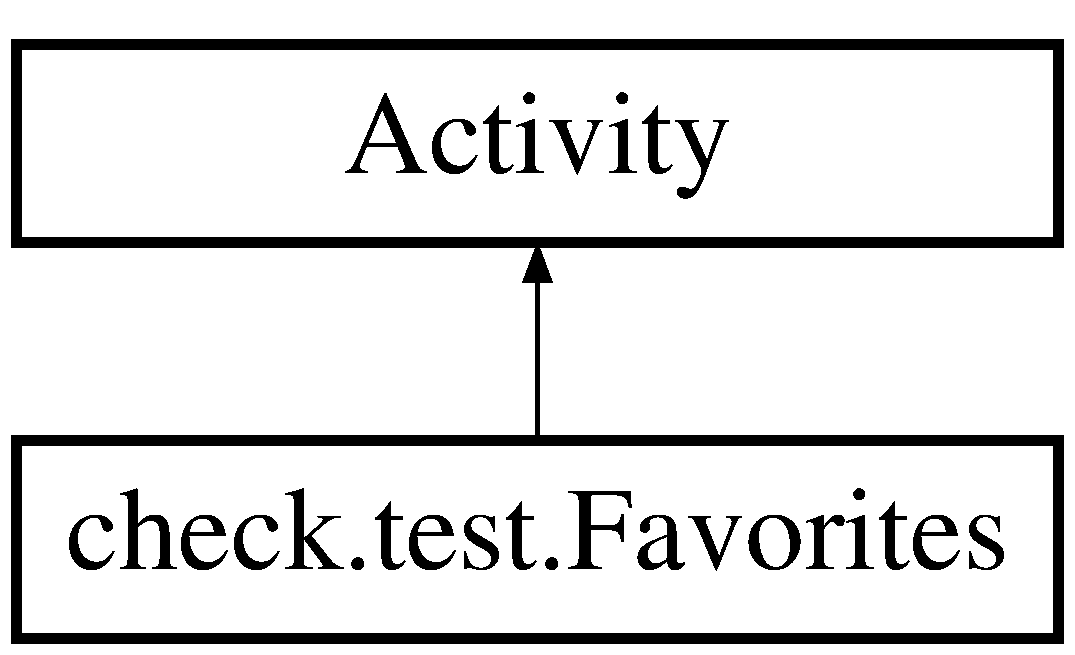
\includegraphics[height=2.000000cm]{classcheck_1_1test_1_1_favorites}
\end{center}
\end{figure}
\subsection*{Protected Member Functions}
\begin{DoxyCompactItemize}
\item 
void \hyperlink{classcheck_1_1test_1_1_favorites_ad3aa3e67369d10b5687cdcfd8bc3a589}{on\+Create} (Bundle saved\+Instance\+State)
\end{DoxyCompactItemize}


\subsection{Detailed Description}
Displays all current saved clothe layouts. 

\subsection{Member Function Documentation}
\hypertarget{classcheck_1_1test_1_1_favorites_ad3aa3e67369d10b5687cdcfd8bc3a589}{}\index{check\+::test\+::\+Favorites@{check\+::test\+::\+Favorites}!on\+Create@{on\+Create}}
\index{on\+Create@{on\+Create}!check\+::test\+::\+Favorites@{check\+::test\+::\+Favorites}}
\subsubsection[{on\+Create(\+Bundle saved\+Instance\+State)}]{\setlength{\rightskip}{0pt plus 5cm}void check.\+test.\+Favorites.\+on\+Create (
\begin{DoxyParamCaption}
\item[{Bundle}]{saved\+Instance\+State}
\end{DoxyParamCaption}
)\hspace{0.3cm}{\ttfamily [protected]}}\label{classcheck_1_1test_1_1_favorites_ad3aa3e67369d10b5687cdcfd8bc3a589}
Get List\+View object from xml

Defined Array values to show in List\+View

List\+View Clicked item index

List\+View Clicked item value

Show Alert 

The documentation for this class was generated from the following file\+:\begin{DoxyCompactItemize}
\item 
C\+:/\+Users/\+Zwretched/.\+Android\+Studio1.\+4/\+Projects/\+Dress\+Me\+\_\+\+Android/\+Dress\+Me/src/main/java/check/test/Favorites.\+java\end{DoxyCompactItemize}

\hypertarget{classcheck_1_1test_1_1_r_1_1id}{}\section{check.\+test.\+R.\+id Class Reference}
\label{classcheck_1_1test_1_1_r_1_1id}\index{check.\+test.\+R.\+id@{check.\+test.\+R.\+id}}
\subsection*{Static Public Attributes}
\begin{DoxyCompactItemize}
\item 
\hypertarget{classcheck_1_1test_1_1_r_1_1id_aa03ba75a03af6646416b8268bc50b51c}{}static final int {\bfseries Favorite\+\_\+\+Profile} =0x7f0c0077\label{classcheck_1_1test_1_1_r_1_1id_aa03ba75a03af6646416b8268bc50b51c}

\item 
\hypertarget{classcheck_1_1test_1_1_r_1_1id_a57a9e2e33ea1698752311ee2f1ab0b5f}{}static final int {\bfseries First\+Button} =0x7f0c0070\label{classcheck_1_1test_1_1_r_1_1id_a57a9e2e33ea1698752311ee2f1ab0b5f}

\item 
\hypertarget{classcheck_1_1test_1_1_r_1_1id_ac553af6d07f7501694b1685a3bbf904b}{}static final int {\bfseries Linear\+Layout02} =0x7f0c0069\label{classcheck_1_1test_1_1_r_1_1id_ac553af6d07f7501694b1685a3bbf904b}

\item 
\hypertarget{classcheck_1_1test_1_1_r_1_1id_a6513a6dad138e2680bfab91c487afb6a}{}static final int {\bfseries Option1} =0x7f0c0088\label{classcheck_1_1test_1_1_r_1_1id_a6513a6dad138e2680bfab91c487afb6a}

\item 
\hypertarget{classcheck_1_1test_1_1_r_1_1id_a717e4776376bda791d0545c9a5048237}{}static final int {\bfseries Option2} =0x7f0c0089\label{classcheck_1_1test_1_1_r_1_1id_a717e4776376bda791d0545c9a5048237}

\item 
\hypertarget{classcheck_1_1test_1_1_r_1_1id_a41cc64fc2a0d148958e5ce5e96df3edb}{}static final int {\bfseries Option3} =0x7f0c008a\label{classcheck_1_1test_1_1_r_1_1id_a41cc64fc2a0d148958e5ce5e96df3edb}

\item 
\hypertarget{classcheck_1_1test_1_1_r_1_1id_a69bc11665be8a9f21a6a99b7407628fd}{}static final int {\bfseries Option4} =0x7f0c008b\label{classcheck_1_1test_1_1_r_1_1id_a69bc11665be8a9f21a6a99b7407628fd}

\item 
\hypertarget{classcheck_1_1test_1_1_r_1_1id_ae06e762572fe73d9d3e5b03c27039f88}{}static final int {\bfseries Option5} =0x7f0c008c\label{classcheck_1_1test_1_1_r_1_1id_ae06e762572fe73d9d3e5b03c27039f88}

\item 
\hypertarget{classcheck_1_1test_1_1_r_1_1id_a2fe0abd6779994053230059068120cac}{}static final int {\bfseries Option6} =0x7f0c008d\label{classcheck_1_1test_1_1_r_1_1id_a2fe0abd6779994053230059068120cac}

\item 
\hypertarget{classcheck_1_1test_1_1_r_1_1id_a1cff9ad823689029201f1b845c877008}{}static final int {\bfseries Profile\+\_\+\+Info} =0x7f0c0078\label{classcheck_1_1test_1_1_r_1_1id_a1cff9ad823689029201f1b845c877008}

\item 
\hypertarget{classcheck_1_1test_1_1_r_1_1id_a3eeb730ea523c06cd1e7a0c4afc1eb1a}{}static final int {\bfseries action} =0x7f0c0079\label{classcheck_1_1test_1_1_r_1_1id_a3eeb730ea523c06cd1e7a0c4afc1eb1a}

\item 
\hypertarget{classcheck_1_1test_1_1_r_1_1id_a0b3c32e9f251a1db16f6bd38d1eb4b1f}{}static final int {\bfseries action0} =0x7f0c007a\label{classcheck_1_1test_1_1_r_1_1id_a0b3c32e9f251a1db16f6bd38d1eb4b1f}

\item 
\hypertarget{classcheck_1_1test_1_1_r_1_1id_ad06caad651634272f387d9ca08f1daaf}{}static final int {\bfseries action\+\_\+bar} =0x7f0c0055\label{classcheck_1_1test_1_1_r_1_1id_ad06caad651634272f387d9ca08f1daaf}

\item 
\hypertarget{classcheck_1_1test_1_1_r_1_1id_af65967f91bdfc834dd2d4ee025af07aa}{}static final int {\bfseries action\+\_\+bar\+\_\+activity\+\_\+content} =0x7f0c0000\label{classcheck_1_1test_1_1_r_1_1id_af65967f91bdfc834dd2d4ee025af07aa}

\item 
\hypertarget{classcheck_1_1test_1_1_r_1_1id_a459283ea26c658d6babacb9943b19681}{}static final int {\bfseries action\+\_\+bar\+\_\+container} =0x7f0c0054\label{classcheck_1_1test_1_1_r_1_1id_a459283ea26c658d6babacb9943b19681}

\item 
\hypertarget{classcheck_1_1test_1_1_r_1_1id_a51408397c0c114e76b4baaf04ce2cc93}{}static final int {\bfseries action\+\_\+bar\+\_\+root} =0x7f0c0050\label{classcheck_1_1test_1_1_r_1_1id_a51408397c0c114e76b4baaf04ce2cc93}

\item 
\hypertarget{classcheck_1_1test_1_1_r_1_1id_ad265e89fb3ef62d7c797275597d36ff4}{}static final int {\bfseries action\+\_\+bar\+\_\+spinner} =0x7f0c0001\label{classcheck_1_1test_1_1_r_1_1id_ad265e89fb3ef62d7c797275597d36ff4}

\item 
\hypertarget{classcheck_1_1test_1_1_r_1_1id_ac73ae0c528d97eb14acf721422abd966}{}static final int {\bfseries action\+\_\+bar\+\_\+subtitle} =0x7f0c0039\label{classcheck_1_1test_1_1_r_1_1id_ac73ae0c528d97eb14acf721422abd966}

\item 
\hypertarget{classcheck_1_1test_1_1_r_1_1id_a17d8da35f0e5aaa54c001de6f92e4da1}{}static final int {\bfseries action\+\_\+bar\+\_\+title} =0x7f0c0038\label{classcheck_1_1test_1_1_r_1_1id_a17d8da35f0e5aaa54c001de6f92e4da1}

\item 
\hypertarget{classcheck_1_1test_1_1_r_1_1id_a9a4f53f1d6e37ac859c473af755a1f29}{}static final int {\bfseries action\+\_\+context\+\_\+bar} =0x7f0c0056\label{classcheck_1_1test_1_1_r_1_1id_a9a4f53f1d6e37ac859c473af755a1f29}

\item 
\hypertarget{classcheck_1_1test_1_1_r_1_1id_a3e7365386f87d86201bdf830c2f2b47c}{}static final int {\bfseries action\+\_\+divider} =0x7f0c007e\label{classcheck_1_1test_1_1_r_1_1id_a3e7365386f87d86201bdf830c2f2b47c}

\item 
\hypertarget{classcheck_1_1test_1_1_r_1_1id_a7e45f724f7702831a8dcb26744db6e55}{}static final int {\bfseries action\+\_\+menu\+\_\+divider} =0x7f0c0002\label{classcheck_1_1test_1_1_r_1_1id_a7e45f724f7702831a8dcb26744db6e55}

\item 
\hypertarget{classcheck_1_1test_1_1_r_1_1id_adc149a649fc021aaaa943b1ab56dbc47}{}static final int {\bfseries action\+\_\+menu\+\_\+presenter} =0x7f0c0003\label{classcheck_1_1test_1_1_r_1_1id_adc149a649fc021aaaa943b1ab56dbc47}

\item 
\hypertarget{classcheck_1_1test_1_1_r_1_1id_ac72e0ce691524564014d0a6eb8ed446a}{}static final int {\bfseries action\+\_\+mode\+\_\+bar} =0x7f0c0052\label{classcheck_1_1test_1_1_r_1_1id_ac72e0ce691524564014d0a6eb8ed446a}

\item 
\hypertarget{classcheck_1_1test_1_1_r_1_1id_a482309978a6eaeb75dc7ae48011f7773}{}static final int {\bfseries action\+\_\+mode\+\_\+bar\+\_\+stub} =0x7f0c0051\label{classcheck_1_1test_1_1_r_1_1id_a482309978a6eaeb75dc7ae48011f7773}

\item 
\hypertarget{classcheck_1_1test_1_1_r_1_1id_aca45b800ebf690292fc70edab489511f}{}static final int {\bfseries action\+\_\+mode\+\_\+close\+\_\+button} =0x7f0c003a\label{classcheck_1_1test_1_1_r_1_1id_aca45b800ebf690292fc70edab489511f}

\item 
\hypertarget{classcheck_1_1test_1_1_r_1_1id_a108532f819897cfefff39e851aae73b0}{}static final int {\bfseries action\+\_\+settings} =0x7f0c0087\label{classcheck_1_1test_1_1_r_1_1id_a108532f819897cfefff39e851aae73b0}

\item 
\hypertarget{classcheck_1_1test_1_1_r_1_1id_a7118354a8560af163e8306e075346821}{}static final int {\bfseries activity\+\_\+chooser\+\_\+view\+\_\+content} =0x7f0c003b\label{classcheck_1_1test_1_1_r_1_1id_a7118354a8560af163e8306e075346821}

\item 
\hypertarget{classcheck_1_1test_1_1_r_1_1id_a81a58c18c61a2a167142c968c63dd938}{}static final int {\bfseries add} =0x7f0c006c\label{classcheck_1_1test_1_1_r_1_1id_a81a58c18c61a2a167142c968c63dd938}

\item 
\hypertarget{classcheck_1_1test_1_1_r_1_1id_aa5d68cdf9842bb79f45c642c403c710b}{}static final int {\bfseries alert\+Title} =0x7f0c0045\label{classcheck_1_1test_1_1_r_1_1id_aa5d68cdf9842bb79f45c642c403c710b}

\item 
\hypertarget{classcheck_1_1test_1_1_r_1_1id_a7deaef9bae4464ee7ad93ca96f69843c}{}static final int {\bfseries always} =0x7f0c0030\label{classcheck_1_1test_1_1_r_1_1id_a7deaef9bae4464ee7ad93ca96f69843c}

\item 
\hypertarget{classcheck_1_1test_1_1_r_1_1id_a027e82ef1ce6e706b36881b84d1acf5f}{}static final int {\bfseries beginning} =0x7f0c002e\label{classcheck_1_1test_1_1_r_1_1id_a027e82ef1ce6e706b36881b84d1acf5f}

\item 
\hypertarget{classcheck_1_1test_1_1_r_1_1id_ac0d6162dadf47d97b5d02be07c9885e8}{}static final int {\bfseries bottom} =0x7f0c001a\label{classcheck_1_1test_1_1_r_1_1id_ac0d6162dadf47d97b5d02be07c9885e8}

\item 
\hypertarget{classcheck_1_1test_1_1_r_1_1id_ac00ea1249f0e80403bacc8b0b3d77cdf}{}static final int {\bfseries button\+Panel} =0x7f0c004b\label{classcheck_1_1test_1_1_r_1_1id_ac00ea1249f0e80403bacc8b0b3d77cdf}

\item 
\hypertarget{classcheck_1_1test_1_1_r_1_1id_a7fd7368809487055fdebd40c75bf476d}{}static final int {\bfseries button\+\_\+accessory} =0x7f0c0066\label{classcheck_1_1test_1_1_r_1_1id_a7fd7368809487055fdebd40c75bf476d}

\item 
\hypertarget{classcheck_1_1test_1_1_r_1_1id_a19d9dd6d40358638f5c492d55909115b}{}static final int {\bfseries button\+\_\+legging} =0x7f0c0067\label{classcheck_1_1test_1_1_r_1_1id_a19d9dd6d40358638f5c492d55909115b}

\item 
\hypertarget{classcheck_1_1test_1_1_r_1_1id_aaa5ad35acc99a61377103a0353f01eef}{}static final int {\bfseries button\+\_\+shoe} =0x7f0c0068\label{classcheck_1_1test_1_1_r_1_1id_aaa5ad35acc99a61377103a0353f01eef}

\item 
\hypertarget{classcheck_1_1test_1_1_r_1_1id_acc3b0aec2dc4980b3358c23ef7de6530}{}static final int {\bfseries button\+\_\+top} =0x7f0c0065\label{classcheck_1_1test_1_1_r_1_1id_acc3b0aec2dc4980b3358c23ef7de6530}

\item 
\hypertarget{classcheck_1_1test_1_1_r_1_1id_a24ec23eea09b2647e4872f4844d95ce7}{}static final int {\bfseries cancel\+\_\+action} =0x7f0c007b\label{classcheck_1_1test_1_1_r_1_1id_a24ec23eea09b2647e4872f4844d95ce7}

\item 
\hypertarget{classcheck_1_1test_1_1_r_1_1id_a47d16fdb74d6941ab35186e45ee28241}{}static final int {\bfseries center} =0x7f0c001b\label{classcheck_1_1test_1_1_r_1_1id_a47d16fdb74d6941ab35186e45ee28241}

\item 
\hypertarget{classcheck_1_1test_1_1_r_1_1id_a6ff08fdec714e2dc615dd8bf2ba1c49f}{}static final int {\bfseries center\+\_\+horizontal} =0x7f0c001c\label{classcheck_1_1test_1_1_r_1_1id_a6ff08fdec714e2dc615dd8bf2ba1c49f}

\item 
\hypertarget{classcheck_1_1test_1_1_r_1_1id_a35f9c48ce05d30319e6bb9c5bd715da1}{}static final int {\bfseries center\+\_\+vertical} =0x7f0c001d\label{classcheck_1_1test_1_1_r_1_1id_a35f9c48ce05d30319e6bb9c5bd715da1}

\item 
\hypertarget{classcheck_1_1test_1_1_r_1_1id_ae9a4630d25eb55cf9b8c0f710f656bc5}{}static final int {\bfseries checkbox} =0x7f0c004d\label{classcheck_1_1test_1_1_r_1_1id_ae9a4630d25eb55cf9b8c0f710f656bc5}

\item 
\hypertarget{classcheck_1_1test_1_1_r_1_1id_abdca1b3b8b09cd9202f418a9560cd94d}{}static final int {\bfseries chronometer} =0x7f0c0081\label{classcheck_1_1test_1_1_r_1_1id_abdca1b3b8b09cd9202f418a9560cd94d}

\item 
\hypertarget{classcheck_1_1test_1_1_r_1_1id_a30b18e9e70cd31288ca03e8919d1edc9}{}static final int {\bfseries clip\+\_\+horizontal} =0x7f0c0029\label{classcheck_1_1test_1_1_r_1_1id_a30b18e9e70cd31288ca03e8919d1edc9}

\item 
\hypertarget{classcheck_1_1test_1_1_r_1_1id_a8af2bfb1a80dac3a08abe583784425bf}{}static final int {\bfseries clip\+\_\+vertical} =0x7f0c002a\label{classcheck_1_1test_1_1_r_1_1id_a8af2bfb1a80dac3a08abe583784425bf}

\item 
\hypertarget{classcheck_1_1test_1_1_r_1_1id_a5f72b85418ccb3fdc71fc6abfaf26652}{}static final int {\bfseries collapse\+Action\+View} =0x7f0c0031\label{classcheck_1_1test_1_1_r_1_1id_a5f72b85418ccb3fdc71fc6abfaf26652}

\item 
\hypertarget{classcheck_1_1test_1_1_r_1_1id_af23e07aa4182f0fc64b8c1add63b5266}{}static final int {\bfseries content\+Panel} =0x7f0c0046\label{classcheck_1_1test_1_1_r_1_1id_af23e07aa4182f0fc64b8c1add63b5266}

\item 
\hypertarget{classcheck_1_1test_1_1_r_1_1id_ae67e1e243cea10cf9f34177a1397144d}{}static final int {\bfseries creation\+\_\+title} =0x7f0c0064\label{classcheck_1_1test_1_1_r_1_1id_ae67e1e243cea10cf9f34177a1397144d}

\item 
\hypertarget{classcheck_1_1test_1_1_r_1_1id_a3c01b17cf4e8c4320b0b572717fb115d}{}static final int {\bfseries custom} =0x7f0c004a\label{classcheck_1_1test_1_1_r_1_1id_a3c01b17cf4e8c4320b0b572717fb115d}

\item 
\hypertarget{classcheck_1_1test_1_1_r_1_1id_a47ea0f7ca58149a9735c3c82b58e24d1}{}static final int {\bfseries custom\+Panel} =0x7f0c0049\label{classcheck_1_1test_1_1_r_1_1id_a47ea0f7ca58149a9735c3c82b58e24d1}

\item 
\hypertarget{classcheck_1_1test_1_1_r_1_1id_a86efd97d588fc2a1950ea33ed3be66af}{}static final int {\bfseries decor\+\_\+content\+\_\+parent} =0x7f0c0053\label{classcheck_1_1test_1_1_r_1_1id_a86efd97d588fc2a1950ea33ed3be66af}

\item 
\hypertarget{classcheck_1_1test_1_1_r_1_1id_a1bb8a6d10462bb8b480ecae0daaecf42}{}static final int {\bfseries default\+\_\+activity\+\_\+button} =0x7f0c003e\label{classcheck_1_1test_1_1_r_1_1id_a1bb8a6d10462bb8b480ecae0daaecf42}

\item 
\hypertarget{classcheck_1_1test_1_1_r_1_1id_ab50c2a91addaa029c0579e53760b67a5}{}static final int {\bfseries disable\+Home} =0x7f0c000d\label{classcheck_1_1test_1_1_r_1_1id_ab50c2a91addaa029c0579e53760b67a5}

\item 
\hypertarget{classcheck_1_1test_1_1_r_1_1id_a9fbb5ad4e727c4f633d2e183defc3359}{}static final int {\bfseries edit\+\_\+query} =0x7f0c0057\label{classcheck_1_1test_1_1_r_1_1id_a9fbb5ad4e727c4f633d2e183defc3359}

\item 
\hypertarget{classcheck_1_1test_1_1_r_1_1id_abfc4b0b9cd4751b496aceb9904caee68}{}static final int {\bfseries end} =0x7f0c001e\label{classcheck_1_1test_1_1_r_1_1id_abfc4b0b9cd4751b496aceb9904caee68}

\item 
\hypertarget{classcheck_1_1test_1_1_r_1_1id_ae946cc108188720a8bc849af2b483d25}{}static final int {\bfseries end\+\_\+padder} =0x7f0c0086\label{classcheck_1_1test_1_1_r_1_1id_ae946cc108188720a8bc849af2b483d25}

\item 
\hypertarget{classcheck_1_1test_1_1_r_1_1id_a7b8dfe43f42c720509349134a7ceb2c0}{}static final int {\bfseries enter\+Always} =0x7f0c0014\label{classcheck_1_1test_1_1_r_1_1id_a7b8dfe43f42c720509349134a7ceb2c0}

\item 
\hypertarget{classcheck_1_1test_1_1_r_1_1id_af0598791be6ca0268c2a3322de86f09e}{}static final int {\bfseries enter\+Always\+Collapsed} =0x7f0c0015\label{classcheck_1_1test_1_1_r_1_1id_af0598791be6ca0268c2a3322de86f09e}

\item 
\hypertarget{classcheck_1_1test_1_1_r_1_1id_a694a2671da85e78873748a9851579479}{}static final int {\bfseries exit\+Until\+Collapsed} =0x7f0c0016\label{classcheck_1_1test_1_1_r_1_1id_a694a2671da85e78873748a9851579479}

\item 
\hypertarget{classcheck_1_1test_1_1_r_1_1id_a0e0399d96462204df85a0d47cc0708bf}{}static final int {\bfseries expand\+\_\+activities\+\_\+button} =0x7f0c003c\label{classcheck_1_1test_1_1_r_1_1id_a0e0399d96462204df85a0d47cc0708bf}

\item 
\hypertarget{classcheck_1_1test_1_1_r_1_1id_a7a1a12bec45a115b37833959399861a8}{}static final int {\bfseries expanded\+\_\+menu} =0x7f0c004c\label{classcheck_1_1test_1_1_r_1_1id_a7a1a12bec45a115b37833959399861a8}

\item 
\hypertarget{classcheck_1_1test_1_1_r_1_1id_a80bedcdd4be9f046c32ecfe4603ca93e}{}static final int {\bfseries favorite} =0x7f0c006a\label{classcheck_1_1test_1_1_r_1_1id_a80bedcdd4be9f046c32ecfe4603ca93e}

\item 
\hypertarget{classcheck_1_1test_1_1_r_1_1id_a6b49737dc9e1752af7bc6f637512446a}{}static final int {\bfseries fill} =0x7f0c002b\label{classcheck_1_1test_1_1_r_1_1id_a6b49737dc9e1752af7bc6f637512446a}

\item 
\hypertarget{classcheck_1_1test_1_1_r_1_1id_a895a6b4d9207d6784d3647d1df3a6150}{}static final int {\bfseries fill\+\_\+horizontal} =0x7f0c002c\label{classcheck_1_1test_1_1_r_1_1id_a895a6b4d9207d6784d3647d1df3a6150}

\item 
\hypertarget{classcheck_1_1test_1_1_r_1_1id_aec55c7d484f7aa4dbea431380cbb82c7}{}static final int {\bfseries fill\+\_\+vertical} =0x7f0c001f\label{classcheck_1_1test_1_1_r_1_1id_aec55c7d484f7aa4dbea431380cbb82c7}

\item 
\hypertarget{classcheck_1_1test_1_1_r_1_1id_a9c9fb6770d652edacf6a7c05061a5390}{}static final int {\bfseries fixed} =0x7f0c0035\label{classcheck_1_1test_1_1_r_1_1id_a9c9fb6770d652edacf6a7c05061a5390}

\item 
\hypertarget{classcheck_1_1test_1_1_r_1_1id_aed38734b6b101d632cc28183589f1b4c}{}static final int {\bfseries gridview} =0x7f0c0071\label{classcheck_1_1test_1_1_r_1_1id_aed38734b6b101d632cc28183589f1b4c}

\item 
\hypertarget{classcheck_1_1test_1_1_r_1_1id_a124687e2f5a2871942d47434effd8f2a}{}static final int {\bfseries home} =0x7f0c0004\label{classcheck_1_1test_1_1_r_1_1id_a124687e2f5a2871942d47434effd8f2a}

\item 
\hypertarget{classcheck_1_1test_1_1_r_1_1id_ac4f7904023f4df7ecdaeca542a7ac388}{}static final int {\bfseries home\+As\+Up} =0x7f0c000e\label{classcheck_1_1test_1_1_r_1_1id_ac4f7904023f4df7ecdaeca542a7ac388}

\item 
\hypertarget{classcheck_1_1test_1_1_r_1_1id_a9ac350f745297f8bc5d4bc7406f91920}{}static final int {\bfseries icon} =0x7f0c0040\label{classcheck_1_1test_1_1_r_1_1id_a9ac350f745297f8bc5d4bc7406f91920}

\item 
\hypertarget{classcheck_1_1test_1_1_r_1_1id_a6d01f76a83bded10315fea5120157ccc}{}static final int {\bfseries if\+Room} =0x7f0c0032\label{classcheck_1_1test_1_1_r_1_1id_a6d01f76a83bded10315fea5120157ccc}

\item 
\hypertarget{classcheck_1_1test_1_1_r_1_1id_ac69d3301973d25cebb1047f322511f0a}{}static final int {\bfseries image} =0x7f0c003d\label{classcheck_1_1test_1_1_r_1_1id_ac69d3301973d25cebb1047f322511f0a}

\item 
\hypertarget{classcheck_1_1test_1_1_r_1_1id_a37c25633da6926f1719de697bceaacb1}{}static final int {\bfseries info} =0x7f0c0085\label{classcheck_1_1test_1_1_r_1_1id_a37c25633da6926f1719de697bceaacb1}

\item 
\hypertarget{classcheck_1_1test_1_1_r_1_1id_a91e3ff57bd43ba2f0ac32b86193569a3}{}static final int {\bfseries left} =0x7f0c0020\label{classcheck_1_1test_1_1_r_1_1id_a91e3ff57bd43ba2f0ac32b86193569a3}

\item 
\hypertarget{classcheck_1_1test_1_1_r_1_1id_a34c26a301479d3d63ab017b5928b0664}{}static final int {\bfseries line1} =0x7f0c007f\label{classcheck_1_1test_1_1_r_1_1id_a34c26a301479d3d63ab017b5928b0664}

\item 
\hypertarget{classcheck_1_1test_1_1_r_1_1id_ad1ef32cf84bce8cbce09091c6da2ba12}{}static final int {\bfseries line3} =0x7f0c0083\label{classcheck_1_1test_1_1_r_1_1id_ad1ef32cf84bce8cbce09091c6da2ba12}

\item 
\hypertarget{classcheck_1_1test_1_1_r_1_1id_a43e44b718481e09aeb801560ab13bc30}{}static final int {\bfseries list} =0x7f0c006f\label{classcheck_1_1test_1_1_r_1_1id_a43e44b718481e09aeb801560ab13bc30}

\item 
\hypertarget{classcheck_1_1test_1_1_r_1_1id_a0a17a661336233846a6b16f797d04825}{}static final int {\bfseries list\+Mode} =0x7f0c000a\label{classcheck_1_1test_1_1_r_1_1id_a0a17a661336233846a6b16f797d04825}

\item 
\hypertarget{classcheck_1_1test_1_1_r_1_1id_add64a82d5c5fdde001b0646fcbef3fe1}{}static final int {\bfseries list\+View\+\_\+grid} =0x7f0c0074\label{classcheck_1_1test_1_1_r_1_1id_add64a82d5c5fdde001b0646fcbef3fe1}

\item 
\hypertarget{classcheck_1_1test_1_1_r_1_1id_a61f549a9ff3eb5d4d65dfaf3d2cf742b}{}static final int {\bfseries list\+\_\+image} =0x7f0c0076\label{classcheck_1_1test_1_1_r_1_1id_a61f549a9ff3eb5d4d65dfaf3d2cf742b}

\item 
\hypertarget{classcheck_1_1test_1_1_r_1_1id_a6e75db552d3dbc1b6284f99d48fcbff7}{}static final int {\bfseries list\+\_\+item} =0x7f0c003f\label{classcheck_1_1test_1_1_r_1_1id_a6e75db552d3dbc1b6284f99d48fcbff7}

\item 
\hypertarget{classcheck_1_1test_1_1_r_1_1id_aca79caabb0f2efef63eb26e1de3bf3a4}{}static final int {\bfseries media\+\_\+actions} =0x7f0c007d\label{classcheck_1_1test_1_1_r_1_1id_aca79caabb0f2efef63eb26e1de3bf3a4}

\item 
\hypertarget{classcheck_1_1test_1_1_r_1_1id_a68f8c8a2446576bb88bde3bdaa8cc0fe}{}static final int {\bfseries middle} =0x7f0c002f\label{classcheck_1_1test_1_1_r_1_1id_a68f8c8a2446576bb88bde3bdaa8cc0fe}

\item 
\hypertarget{classcheck_1_1test_1_1_r_1_1id_ae0085f407b6620b87816e74176c87d49}{}static final int {\bfseries mini} =0x7f0c002d\label{classcheck_1_1test_1_1_r_1_1id_ae0085f407b6620b87816e74176c87d49}

\item 
\hypertarget{classcheck_1_1test_1_1_r_1_1id_a01213b9e224ef1404cc8f21ec6e46196}{}static final int {\bfseries multiply} =0x7f0c0024\label{classcheck_1_1test_1_1_r_1_1id_a01213b9e224ef1404cc8f21ec6e46196}

\item 
\hypertarget{classcheck_1_1test_1_1_r_1_1id_a7442d9a0506155fbc572a2f456360b96}{}static final int {\bfseries never} =0x7f0c0033\label{classcheck_1_1test_1_1_r_1_1id_a7442d9a0506155fbc572a2f456360b96}

\item 
\hypertarget{classcheck_1_1test_1_1_r_1_1id_a2d24eeb168ce61c3227451d342cb7c50}{}static final int {\bfseries none} =0x7f0c000f\label{classcheck_1_1test_1_1_r_1_1id_a2d24eeb168ce61c3227451d342cb7c50}

\item 
\hypertarget{classcheck_1_1test_1_1_r_1_1id_a20815d2596774915df34523c64def2d1}{}static final int {\bfseries normal} =0x7f0c000b\label{classcheck_1_1test_1_1_r_1_1id_a20815d2596774915df34523c64def2d1}

\item 
\hypertarget{classcheck_1_1test_1_1_r_1_1id_afddd81c642a5abdfff02d3628e3af9a3}{}static final int {\bfseries parallax} =0x7f0c0018\label{classcheck_1_1test_1_1_r_1_1id_afddd81c642a5abdfff02d3628e3af9a3}

\item 
\hypertarget{classcheck_1_1test_1_1_r_1_1id_a8b5d1beeedf525a644165c9400dd4f6a}{}static final int {\bfseries parent\+Panel} =0x7f0c0042\label{classcheck_1_1test_1_1_r_1_1id_a8b5d1beeedf525a644165c9400dd4f6a}

\item 
\hypertarget{classcheck_1_1test_1_1_r_1_1id_a2626a27c5b1a35902534be25ae442940}{}static final int {\bfseries pin} =0x7f0c0019\label{classcheck_1_1test_1_1_r_1_1id_a2626a27c5b1a35902534be25ae442940}

\item 
\hypertarget{classcheck_1_1test_1_1_r_1_1id_aa511dff275f098da369213fbd508896e}{}static final int {\bfseries progress\+\_\+circular} =0x7f0c0005\label{classcheck_1_1test_1_1_r_1_1id_aa511dff275f098da369213fbd508896e}

\item 
\hypertarget{classcheck_1_1test_1_1_r_1_1id_aefb86c4a08d2691d793eee498e241d31}{}static final int {\bfseries progress\+\_\+horizontal} =0x7f0c0006\label{classcheck_1_1test_1_1_r_1_1id_aefb86c4a08d2691d793eee498e241d31}

\item 
\hypertarget{classcheck_1_1test_1_1_r_1_1id_a820fe6049a102cc029fd9ac8621a4492}{}static final int {\bfseries radio} =0x7f0c004f\label{classcheck_1_1test_1_1_r_1_1id_a820fe6049a102cc029fd9ac8621a4492}

\item 
\hypertarget{classcheck_1_1test_1_1_r_1_1id_ad8c21a9585844a9c5248147141ef1245}{}static final int {\bfseries randomize} =0x7f0c006d\label{classcheck_1_1test_1_1_r_1_1id_ad8c21a9585844a9c5248147141ef1245}

\item 
\hypertarget{classcheck_1_1test_1_1_r_1_1id_a7c9ffb76d82d7711d0fd9fbf2568d74a}{}static final int {\bfseries right} =0x7f0c0021\label{classcheck_1_1test_1_1_r_1_1id_a7c9ffb76d82d7711d0fd9fbf2568d74a}

\item 
\hypertarget{classcheck_1_1test_1_1_r_1_1id_a1e2042b2501a69a60172ea59493bd21b}{}static final int {\bfseries screen} =0x7f0c0025\label{classcheck_1_1test_1_1_r_1_1id_a1e2042b2501a69a60172ea59493bd21b}

\item 
\hypertarget{classcheck_1_1test_1_1_r_1_1id_a886d2803a7bc74d5d3cde397900e475e}{}static final int {\bfseries scroll} =0x7f0c0017\label{classcheck_1_1test_1_1_r_1_1id_a886d2803a7bc74d5d3cde397900e475e}

\item 
\hypertarget{classcheck_1_1test_1_1_r_1_1id_abe0c909efca23f5b9c323c7f4c3eb93c}{}static final int {\bfseries scroll\+View} =0x7f0c0047\label{classcheck_1_1test_1_1_r_1_1id_abe0c909efca23f5b9c323c7f4c3eb93c}

\item 
\hypertarget{classcheck_1_1test_1_1_r_1_1id_abf8adc57816943b2b0bbf61f635a05c2}{}static final int {\bfseries scrollable} =0x7f0c0036\label{classcheck_1_1test_1_1_r_1_1id_abf8adc57816943b2b0bbf61f635a05c2}

\item 
\hypertarget{classcheck_1_1test_1_1_r_1_1id_af0f43b87dbc6a20eaf9a7b6e90ffb42e}{}static final int {\bfseries search\+\_\+badge} =0x7f0c0059\label{classcheck_1_1test_1_1_r_1_1id_af0f43b87dbc6a20eaf9a7b6e90ffb42e}

\item 
\hypertarget{classcheck_1_1test_1_1_r_1_1id_a2c6e9dfb9e176d7a45e47660e08c0068}{}static final int {\bfseries search\+\_\+bar} =0x7f0c0058\label{classcheck_1_1test_1_1_r_1_1id_a2c6e9dfb9e176d7a45e47660e08c0068}

\item 
\hypertarget{classcheck_1_1test_1_1_r_1_1id_ad526646a4ec25af099e031c7ec09d638}{}static final int {\bfseries search\+\_\+button} =0x7f0c005a\label{classcheck_1_1test_1_1_r_1_1id_ad526646a4ec25af099e031c7ec09d638}

\item 
\hypertarget{classcheck_1_1test_1_1_r_1_1id_a81fd34df73f183d3ea044d8da43e3371}{}static final int {\bfseries search\+\_\+close\+\_\+btn} =0x7f0c005f\label{classcheck_1_1test_1_1_r_1_1id_a81fd34df73f183d3ea044d8da43e3371}

\item 
\hypertarget{classcheck_1_1test_1_1_r_1_1id_a16e72c1679bb7f9c13e5dd3e6f9adcb8}{}static final int {\bfseries search\+\_\+edit\+\_\+frame} =0x7f0c005b\label{classcheck_1_1test_1_1_r_1_1id_a16e72c1679bb7f9c13e5dd3e6f9adcb8}

\item 
\hypertarget{classcheck_1_1test_1_1_r_1_1id_aa307f16f2e0b749e9191a15241a0b562}{}static final int {\bfseries search\+\_\+go\+\_\+btn} =0x7f0c0061\label{classcheck_1_1test_1_1_r_1_1id_aa307f16f2e0b749e9191a15241a0b562}

\item 
\hypertarget{classcheck_1_1test_1_1_r_1_1id_a56111d9f3bc6ffe56b659968717d7c51}{}static final int {\bfseries search\+\_\+mag\+\_\+icon} =0x7f0c005c\label{classcheck_1_1test_1_1_r_1_1id_a56111d9f3bc6ffe56b659968717d7c51}

\item 
\hypertarget{classcheck_1_1test_1_1_r_1_1id_afbe0678813dad6eea29e5afdddaa81e7}{}static final int {\bfseries search\+\_\+plate} =0x7f0c005d\label{classcheck_1_1test_1_1_r_1_1id_afbe0678813dad6eea29e5afdddaa81e7}

\item 
\hypertarget{classcheck_1_1test_1_1_r_1_1id_a3494f315ed5563a71b53aca71ff55f03}{}static final int {\bfseries search\+\_\+src\+\_\+text} =0x7f0c005e\label{classcheck_1_1test_1_1_r_1_1id_a3494f315ed5563a71b53aca71ff55f03}

\item 
\hypertarget{classcheck_1_1test_1_1_r_1_1id_a07ff2b7bbdc1d835556d534600887751}{}static final int {\bfseries search\+\_\+voice\+\_\+btn} =0x7f0c0062\label{classcheck_1_1test_1_1_r_1_1id_a07ff2b7bbdc1d835556d534600887751}

\item 
\hypertarget{classcheck_1_1test_1_1_r_1_1id_ad85d3d582fac3b51e9d70f5be944d8de}{}static final int {\bfseries select\+\_\+dialog\+\_\+listview} =0x7f0c0063\label{classcheck_1_1test_1_1_r_1_1id_ad85d3d582fac3b51e9d70f5be944d8de}

\item 
\hypertarget{classcheck_1_1test_1_1_r_1_1id_aad0f6a37d175a3aa1b919e668fff34d8}{}static final int {\bfseries shortcut} =0x7f0c004e\label{classcheck_1_1test_1_1_r_1_1id_aad0f6a37d175a3aa1b919e668fff34d8}

\item 
\hypertarget{classcheck_1_1test_1_1_r_1_1id_a2c133929ef60295d5d0633c24d59678a}{}static final int {\bfseries show\+Custom} =0x7f0c0010\label{classcheck_1_1test_1_1_r_1_1id_a2c133929ef60295d5d0633c24d59678a}

\item 
\hypertarget{classcheck_1_1test_1_1_r_1_1id_a6ae31d8708ef22d0ea4e769029a6abe8}{}static final int {\bfseries show\+Home} =0x7f0c0011\label{classcheck_1_1test_1_1_r_1_1id_a6ae31d8708ef22d0ea4e769029a6abe8}

\item 
\hypertarget{classcheck_1_1test_1_1_r_1_1id_a65a54356a295f4aa187dda3abf16b509}{}static final int {\bfseries show\+Title} =0x7f0c0012\label{classcheck_1_1test_1_1_r_1_1id_a65a54356a295f4aa187dda3abf16b509}

\item 
\hypertarget{classcheck_1_1test_1_1_r_1_1id_ac7ffd14f26cc22af42fa287330369e95}{}static final int {\bfseries snackbar\+\_\+action} =0x7f0c0073\label{classcheck_1_1test_1_1_r_1_1id_ac7ffd14f26cc22af42fa287330369e95}

\item 
\hypertarget{classcheck_1_1test_1_1_r_1_1id_aa93fe9cc375175eeb67a389f23942e47}{}static final int {\bfseries snackbar\+\_\+text} =0x7f0c0072\label{classcheck_1_1test_1_1_r_1_1id_aa93fe9cc375175eeb67a389f23942e47}

\item 
\hypertarget{classcheck_1_1test_1_1_r_1_1id_ab08b5a0414247affe40f9cd4cd0745fe}{}static final int {\bfseries split\+\_\+action\+\_\+bar} =0x7f0c0007\label{classcheck_1_1test_1_1_r_1_1id_ab08b5a0414247affe40f9cd4cd0745fe}

\item 
\hypertarget{classcheck_1_1test_1_1_r_1_1id_aba9850174bcec6d73373e7df7c84ebd2}{}static final int {\bfseries src\+\_\+atop} =0x7f0c0026\label{classcheck_1_1test_1_1_r_1_1id_aba9850174bcec6d73373e7df7c84ebd2}

\item 
\hypertarget{classcheck_1_1test_1_1_r_1_1id_aca22566a14f1c02d0ef5150234769eef}{}static final int {\bfseries src\+\_\+in} =0x7f0c0027\label{classcheck_1_1test_1_1_r_1_1id_aca22566a14f1c02d0ef5150234769eef}

\item 
\hypertarget{classcheck_1_1test_1_1_r_1_1id_aafecc3d70897982f7ee92a471f5b0bb9}{}static final int {\bfseries src\+\_\+over} =0x7f0c0028\label{classcheck_1_1test_1_1_r_1_1id_aafecc3d70897982f7ee92a471f5b0bb9}

\item 
\hypertarget{classcheck_1_1test_1_1_r_1_1id_a79e65c221060bc2287ca3d62b8094b99}{}static final int {\bfseries start} =0x7f0c0022\label{classcheck_1_1test_1_1_r_1_1id_a79e65c221060bc2287ca3d62b8094b99}

\item 
\hypertarget{classcheck_1_1test_1_1_r_1_1id_ae18ac3d7350855442f47a1552de0626e}{}static final int {\bfseries status\+\_\+bar\+\_\+latest\+\_\+event\+\_\+content} =0x7f0c007c\label{classcheck_1_1test_1_1_r_1_1id_ae18ac3d7350855442f47a1552de0626e}

\item 
\hypertarget{classcheck_1_1test_1_1_r_1_1id_a6fd3789ecb8fa908863403a8e282a901}{}static final int {\bfseries submit\+\_\+area} =0x7f0c0060\label{classcheck_1_1test_1_1_r_1_1id_a6fd3789ecb8fa908863403a8e282a901}

\item 
\hypertarget{classcheck_1_1test_1_1_r_1_1id_a2e5b94af0bcde09931e29bca1fa6e8bb}{}static final int {\bfseries tab\+Mode} =0x7f0c000c\label{classcheck_1_1test_1_1_r_1_1id_a2e5b94af0bcde09931e29bca1fa6e8bb}

\item 
\hypertarget{classcheck_1_1test_1_1_r_1_1id_ade0af31f3a713b41343b1491e95f98b5}{}static final int {\bfseries text} =0x7f0c0084\label{classcheck_1_1test_1_1_r_1_1id_ade0af31f3a713b41343b1491e95f98b5}

\item 
\hypertarget{classcheck_1_1test_1_1_r_1_1id_a6594515b6f17b2d51bab81ab7ca565cf}{}static final int {\bfseries text2} =0x7f0c0082\label{classcheck_1_1test_1_1_r_1_1id_a6594515b6f17b2d51bab81ab7ca565cf}

\item 
\hypertarget{classcheck_1_1test_1_1_r_1_1id_ab9c9d3e34a93e61aafa1dd0b78348a9f}{}static final int {\bfseries text\+Spacer\+No\+Buttons} =0x7f0c0048\label{classcheck_1_1test_1_1_r_1_1id_ab9c9d3e34a93e61aafa1dd0b78348a9f}

\item 
\hypertarget{classcheck_1_1test_1_1_r_1_1id_a890feb897925907af46c11ee11021b5c}{}static final int {\bfseries thumbnail} =0x7f0c0075\label{classcheck_1_1test_1_1_r_1_1id_a890feb897925907af46c11ee11021b5c}

\item 
\hypertarget{classcheck_1_1test_1_1_r_1_1id_a1f760c0ac24bade7599bfb4e808cce10}{}static final int {\bfseries time} =0x7f0c0080\label{classcheck_1_1test_1_1_r_1_1id_a1f760c0ac24bade7599bfb4e808cce10}

\item 
\hypertarget{classcheck_1_1test_1_1_r_1_1id_a22809e30ef7672e73075e3d2c4424fd3}{}static final int {\bfseries title} =0x7f0c0041\label{classcheck_1_1test_1_1_r_1_1id_a22809e30ef7672e73075e3d2c4424fd3}

\item 
\hypertarget{classcheck_1_1test_1_1_r_1_1id_abb9713147f40052ece7a17bffee8739d}{}static final int {\bfseries title\+\_\+template} =0x7f0c0044\label{classcheck_1_1test_1_1_r_1_1id_abb9713147f40052ece7a17bffee8739d}

\item 
\hypertarget{classcheck_1_1test_1_1_r_1_1id_af2d5df0c49bdc4a19f7c924595f83c11}{}static final int {\bfseries top} =0x7f0c0023\label{classcheck_1_1test_1_1_r_1_1id_af2d5df0c49bdc4a19f7c924595f83c11}

\item 
\hypertarget{classcheck_1_1test_1_1_r_1_1id_ad0d7328f822ffbc8e5e4f5d0cbfd6c9b}{}static final int {\bfseries top\+Panel} =0x7f0c0043\label{classcheck_1_1test_1_1_r_1_1id_ad0d7328f822ffbc8e5e4f5d0cbfd6c9b}

\item 
\hypertarget{classcheck_1_1test_1_1_r_1_1id_a1ad083411c099a92474d9da49e8efebe}{}static final int {\bfseries up} =0x7f0c0008\label{classcheck_1_1test_1_1_r_1_1id_a1ad083411c099a92474d9da49e8efebe}

\item 
\hypertarget{classcheck_1_1test_1_1_r_1_1id_ae4631fbbe86141d9c87bbcbb260ff34b}{}static final int {\bfseries upload} =0x7f0c006e\label{classcheck_1_1test_1_1_r_1_1id_ae4631fbbe86141d9c87bbcbb260ff34b}

\item 
\hypertarget{classcheck_1_1test_1_1_r_1_1id_a4587012d77ca2319bb52864458dd53cc}{}static final int {\bfseries use\+Logo} =0x7f0c0013\label{classcheck_1_1test_1_1_r_1_1id_a4587012d77ca2319bb52864458dd53cc}

\item 
\hypertarget{classcheck_1_1test_1_1_r_1_1id_a9ad0b1af436614ea93630e231bbc28ff}{}static final int {\bfseries view\+\_\+offset\+\_\+helper} =0x7f0c0009\label{classcheck_1_1test_1_1_r_1_1id_a9ad0b1af436614ea93630e231bbc28ff}

\item 
\hypertarget{classcheck_1_1test_1_1_r_1_1id_a3dc69afb622c2b786a3c150088261292}{}static final int {\bfseries weather} =0x7f0c006b\label{classcheck_1_1test_1_1_r_1_1id_a3dc69afb622c2b786a3c150088261292}

\item 
\hypertarget{classcheck_1_1test_1_1_r_1_1id_a6c8121872834b364de9ec0c1b858d30c}{}static final int {\bfseries with\+Text} =0x7f0c0034\label{classcheck_1_1test_1_1_r_1_1id_a6c8121872834b364de9ec0c1b858d30c}

\item 
\hypertarget{classcheck_1_1test_1_1_r_1_1id_aebcfb6a3b83a26f94745bf11ba7581b2}{}static final int {\bfseries wrap\+\_\+content} =0x7f0c0037\label{classcheck_1_1test_1_1_r_1_1id_aebcfb6a3b83a26f94745bf11ba7581b2}

\end{DoxyCompactItemize}


The documentation for this class was generated from the following file\+:\begin{DoxyCompactItemize}
\item 
C\+:/\+Users/\+Zwretched/.\+Android\+Studio1.\+4/\+Projects/\+Dress\+Me\+\_\+\+Android/\+Dress\+Me/build/generated/source/r/debug/check/test/R.\+java\end{DoxyCompactItemize}

\hypertarget{classandroid_1_1support_1_1v7_1_1appcompat_1_1_r_1_1id}{}\section{android.\+support.\+v7.\+appcompat.\+R.\+id Class Reference}
\label{classandroid_1_1support_1_1v7_1_1appcompat_1_1_r_1_1id}\index{android.\+support.\+v7.\+appcompat.\+R.\+id@{android.\+support.\+v7.\+appcompat.\+R.\+id}}
\subsection*{Static Public Attributes}
\begin{DoxyCompactItemize}
\item 
\hypertarget{classandroid_1_1support_1_1v7_1_1appcompat_1_1_r_1_1id_a2c658ecf3cb7a212407850bf58715caa}{}static final int {\bfseries action0} = 0x7f0c007a\label{classandroid_1_1support_1_1v7_1_1appcompat_1_1_r_1_1id_a2c658ecf3cb7a212407850bf58715caa}

\item 
\hypertarget{classandroid_1_1support_1_1v7_1_1appcompat_1_1_r_1_1id_a6c9c8b18c3b57617cf60a9b1ad51f2f1}{}static final int {\bfseries action\+\_\+bar} = 0x7f0c0055\label{classandroid_1_1support_1_1v7_1_1appcompat_1_1_r_1_1id_a6c9c8b18c3b57617cf60a9b1ad51f2f1}

\item 
\hypertarget{classandroid_1_1support_1_1v7_1_1appcompat_1_1_r_1_1id_a9ed5ea10a253071eaefa58062f541097}{}static final int {\bfseries action\+\_\+bar\+\_\+activity\+\_\+content} = 0x7f0c0000\label{classandroid_1_1support_1_1v7_1_1appcompat_1_1_r_1_1id_a9ed5ea10a253071eaefa58062f541097}

\item 
\hypertarget{classandroid_1_1support_1_1v7_1_1appcompat_1_1_r_1_1id_a4e19d90e373b2bdb18641e8820c0d7a3}{}static final int {\bfseries action\+\_\+bar\+\_\+container} = 0x7f0c0054\label{classandroid_1_1support_1_1v7_1_1appcompat_1_1_r_1_1id_a4e19d90e373b2bdb18641e8820c0d7a3}

\item 
\hypertarget{classandroid_1_1support_1_1v7_1_1appcompat_1_1_r_1_1id_afbd1bfdb4a6c3f4fe61c7d6f8d0b6f45}{}static final int {\bfseries action\+\_\+bar\+\_\+root} = 0x7f0c0050\label{classandroid_1_1support_1_1v7_1_1appcompat_1_1_r_1_1id_afbd1bfdb4a6c3f4fe61c7d6f8d0b6f45}

\item 
\hypertarget{classandroid_1_1support_1_1v7_1_1appcompat_1_1_r_1_1id_ae703f67eed43afe20bafdd104fc16078}{}static final int {\bfseries action\+\_\+bar\+\_\+spinner} = 0x7f0c0001\label{classandroid_1_1support_1_1v7_1_1appcompat_1_1_r_1_1id_ae703f67eed43afe20bafdd104fc16078}

\item 
\hypertarget{classandroid_1_1support_1_1v7_1_1appcompat_1_1_r_1_1id_ac071fd37a9fcb4d4f8f4179f7d722e40}{}static final int {\bfseries action\+\_\+bar\+\_\+subtitle} = 0x7f0c0039\label{classandroid_1_1support_1_1v7_1_1appcompat_1_1_r_1_1id_ac071fd37a9fcb4d4f8f4179f7d722e40}

\item 
\hypertarget{classandroid_1_1support_1_1v7_1_1appcompat_1_1_r_1_1id_a30bf2ad178d05c2a1633b54e55ed8e8a}{}static final int {\bfseries action\+\_\+bar\+\_\+title} = 0x7f0c0038\label{classandroid_1_1support_1_1v7_1_1appcompat_1_1_r_1_1id_a30bf2ad178d05c2a1633b54e55ed8e8a}

\item 
\hypertarget{classandroid_1_1support_1_1v7_1_1appcompat_1_1_r_1_1id_ad1965908d64ef4efb15b3160636a5ed8}{}static final int {\bfseries action\+\_\+context\+\_\+bar} = 0x7f0c0056\label{classandroid_1_1support_1_1v7_1_1appcompat_1_1_r_1_1id_ad1965908d64ef4efb15b3160636a5ed8}

\item 
\hypertarget{classandroid_1_1support_1_1v7_1_1appcompat_1_1_r_1_1id_a0a3104dca1878dbe491df3b2a159b926}{}static final int {\bfseries action\+\_\+divider} = 0x7f0c007e\label{classandroid_1_1support_1_1v7_1_1appcompat_1_1_r_1_1id_a0a3104dca1878dbe491df3b2a159b926}

\item 
\hypertarget{classandroid_1_1support_1_1v7_1_1appcompat_1_1_r_1_1id_ac6f27784f564da74cdbfc67d6cd3137a}{}static final int {\bfseries action\+\_\+menu\+\_\+divider} = 0x7f0c0002\label{classandroid_1_1support_1_1v7_1_1appcompat_1_1_r_1_1id_ac6f27784f564da74cdbfc67d6cd3137a}

\item 
\hypertarget{classandroid_1_1support_1_1v7_1_1appcompat_1_1_r_1_1id_ab66934cd579e0cdffbb6fe852773d3ed}{}static final int {\bfseries action\+\_\+menu\+\_\+presenter} = 0x7f0c0003\label{classandroid_1_1support_1_1v7_1_1appcompat_1_1_r_1_1id_ab66934cd579e0cdffbb6fe852773d3ed}

\item 
\hypertarget{classandroid_1_1support_1_1v7_1_1appcompat_1_1_r_1_1id_a2f1bb6e3c76848980dee3e5b042a636e}{}static final int {\bfseries action\+\_\+mode\+\_\+bar} = 0x7f0c0052\label{classandroid_1_1support_1_1v7_1_1appcompat_1_1_r_1_1id_a2f1bb6e3c76848980dee3e5b042a636e}

\item 
\hypertarget{classandroid_1_1support_1_1v7_1_1appcompat_1_1_r_1_1id_a8f0e0b57baf177d6e5eeae0998ec7e80}{}static final int {\bfseries action\+\_\+mode\+\_\+bar\+\_\+stub} = 0x7f0c0051\label{classandroid_1_1support_1_1v7_1_1appcompat_1_1_r_1_1id_a8f0e0b57baf177d6e5eeae0998ec7e80}

\item 
\hypertarget{classandroid_1_1support_1_1v7_1_1appcompat_1_1_r_1_1id_ae146768e3a755580d17b7afbcd4def28}{}static final int {\bfseries action\+\_\+mode\+\_\+close\+\_\+button} = 0x7f0c003a\label{classandroid_1_1support_1_1v7_1_1appcompat_1_1_r_1_1id_ae146768e3a755580d17b7afbcd4def28}

\item 
\hypertarget{classandroid_1_1support_1_1v7_1_1appcompat_1_1_r_1_1id_af98faa6b183536adf4a34e5131811132}{}static final int {\bfseries activity\+\_\+chooser\+\_\+view\+\_\+content} = 0x7f0c003b\label{classandroid_1_1support_1_1v7_1_1appcompat_1_1_r_1_1id_af98faa6b183536adf4a34e5131811132}

\item 
\hypertarget{classandroid_1_1support_1_1v7_1_1appcompat_1_1_r_1_1id_ad40c53e1bf9fa8b9f6f57d83f4b4d1a1}{}static final int {\bfseries alert\+Title} = 0x7f0c0045\label{classandroid_1_1support_1_1v7_1_1appcompat_1_1_r_1_1id_ad40c53e1bf9fa8b9f6f57d83f4b4d1a1}

\item 
\hypertarget{classandroid_1_1support_1_1v7_1_1appcompat_1_1_r_1_1id_aa777b276e6d57dbc1483dd37ea9c433e}{}static final int {\bfseries always} = 0x7f0c0030\label{classandroid_1_1support_1_1v7_1_1appcompat_1_1_r_1_1id_aa777b276e6d57dbc1483dd37ea9c433e}

\item 
\hypertarget{classandroid_1_1support_1_1v7_1_1appcompat_1_1_r_1_1id_ac0d21579074d2c5dd27041e24c9deb9e}{}static final int {\bfseries beginning} = 0x7f0c002e\label{classandroid_1_1support_1_1v7_1_1appcompat_1_1_r_1_1id_ac0d21579074d2c5dd27041e24c9deb9e}

\item 
\hypertarget{classandroid_1_1support_1_1v7_1_1appcompat_1_1_r_1_1id_a54c250694e2e32d9d0bffc4eb06c2a7c}{}static final int {\bfseries button\+Panel} = 0x7f0c004b\label{classandroid_1_1support_1_1v7_1_1appcompat_1_1_r_1_1id_a54c250694e2e32d9d0bffc4eb06c2a7c}

\item 
\hypertarget{classandroid_1_1support_1_1v7_1_1appcompat_1_1_r_1_1id_a8eed8129813c0adb484ad6906f6f2273}{}static final int {\bfseries cancel\+\_\+action} = 0x7f0c007b\label{classandroid_1_1support_1_1v7_1_1appcompat_1_1_r_1_1id_a8eed8129813c0adb484ad6906f6f2273}

\item 
\hypertarget{classandroid_1_1support_1_1v7_1_1appcompat_1_1_r_1_1id_ace6d05a8aeb5fac518dcec95ece0b4c2}{}static final int {\bfseries checkbox} = 0x7f0c004d\label{classandroid_1_1support_1_1v7_1_1appcompat_1_1_r_1_1id_ace6d05a8aeb5fac518dcec95ece0b4c2}

\item 
\hypertarget{classandroid_1_1support_1_1v7_1_1appcompat_1_1_r_1_1id_afb6264939cc20738a3bda59526ecfdc6}{}static final int {\bfseries chronometer} = 0x7f0c0081\label{classandroid_1_1support_1_1v7_1_1appcompat_1_1_r_1_1id_afb6264939cc20738a3bda59526ecfdc6}

\item 
\hypertarget{classandroid_1_1support_1_1v7_1_1appcompat_1_1_r_1_1id_a40ae047cbae54b193b8c459b4f21b6bb}{}static final int {\bfseries collapse\+Action\+View} = 0x7f0c0031\label{classandroid_1_1support_1_1v7_1_1appcompat_1_1_r_1_1id_a40ae047cbae54b193b8c459b4f21b6bb}

\item 
\hypertarget{classandroid_1_1support_1_1v7_1_1appcompat_1_1_r_1_1id_a7ca9a7024cb6cfea705fe251a7e4a3ab}{}static final int {\bfseries content\+Panel} = 0x7f0c0046\label{classandroid_1_1support_1_1v7_1_1appcompat_1_1_r_1_1id_a7ca9a7024cb6cfea705fe251a7e4a3ab}

\item 
\hypertarget{classandroid_1_1support_1_1v7_1_1appcompat_1_1_r_1_1id_a42c3f8858afe9accbfb229c5a0470024}{}static final int {\bfseries custom} = 0x7f0c004a\label{classandroid_1_1support_1_1v7_1_1appcompat_1_1_r_1_1id_a42c3f8858afe9accbfb229c5a0470024}

\item 
\hypertarget{classandroid_1_1support_1_1v7_1_1appcompat_1_1_r_1_1id_a4f4e1a3faa478db1183ae51c17dcff31}{}static final int {\bfseries custom\+Panel} = 0x7f0c0049\label{classandroid_1_1support_1_1v7_1_1appcompat_1_1_r_1_1id_a4f4e1a3faa478db1183ae51c17dcff31}

\item 
\hypertarget{classandroid_1_1support_1_1v7_1_1appcompat_1_1_r_1_1id_aea0320decb2f530b61643c8b8398f559}{}static final int {\bfseries decor\+\_\+content\+\_\+parent} = 0x7f0c0053\label{classandroid_1_1support_1_1v7_1_1appcompat_1_1_r_1_1id_aea0320decb2f530b61643c8b8398f559}

\item 
\hypertarget{classandroid_1_1support_1_1v7_1_1appcompat_1_1_r_1_1id_a744e60e505fa071f1cc339c813393086}{}static final int {\bfseries default\+\_\+activity\+\_\+button} = 0x7f0c003e\label{classandroid_1_1support_1_1v7_1_1appcompat_1_1_r_1_1id_a744e60e505fa071f1cc339c813393086}

\item 
\hypertarget{classandroid_1_1support_1_1v7_1_1appcompat_1_1_r_1_1id_a2ea479dc51c28dcc42c7ca7d208d0d6e}{}static final int {\bfseries disable\+Home} = 0x7f0c000d\label{classandroid_1_1support_1_1v7_1_1appcompat_1_1_r_1_1id_a2ea479dc51c28dcc42c7ca7d208d0d6e}

\item 
\hypertarget{classandroid_1_1support_1_1v7_1_1appcompat_1_1_r_1_1id_af94f57ae49bc17ea306089567ef89794}{}static final int {\bfseries edit\+\_\+query} = 0x7f0c0057\label{classandroid_1_1support_1_1v7_1_1appcompat_1_1_r_1_1id_af94f57ae49bc17ea306089567ef89794}

\item 
\hypertarget{classandroid_1_1support_1_1v7_1_1appcompat_1_1_r_1_1id_aac9afcc19f505681aa88202a7b27d31e}{}static final int {\bfseries end} = 0x7f0c001e\label{classandroid_1_1support_1_1v7_1_1appcompat_1_1_r_1_1id_aac9afcc19f505681aa88202a7b27d31e}

\item 
\hypertarget{classandroid_1_1support_1_1v7_1_1appcompat_1_1_r_1_1id_ade99771836755a53a58fb2525d0b5792}{}static final int {\bfseries end\+\_\+padder} = 0x7f0c0086\label{classandroid_1_1support_1_1v7_1_1appcompat_1_1_r_1_1id_ade99771836755a53a58fb2525d0b5792}

\item 
\hypertarget{classandroid_1_1support_1_1v7_1_1appcompat_1_1_r_1_1id_a322929fd47d9215e3b10b62d3762f5eb}{}static final int {\bfseries expand\+\_\+activities\+\_\+button} = 0x7f0c003c\label{classandroid_1_1support_1_1v7_1_1appcompat_1_1_r_1_1id_a322929fd47d9215e3b10b62d3762f5eb}

\item 
\hypertarget{classandroid_1_1support_1_1v7_1_1appcompat_1_1_r_1_1id_a3aa9e89f2cfd5dd834212e9e9d185a81}{}static final int {\bfseries expanded\+\_\+menu} = 0x7f0c004c\label{classandroid_1_1support_1_1v7_1_1appcompat_1_1_r_1_1id_a3aa9e89f2cfd5dd834212e9e9d185a81}

\item 
\hypertarget{classandroid_1_1support_1_1v7_1_1appcompat_1_1_r_1_1id_acedb19aa69792f84b956f8fb7cc4b972}{}static final int {\bfseries home} = 0x7f0c0004\label{classandroid_1_1support_1_1v7_1_1appcompat_1_1_r_1_1id_acedb19aa69792f84b956f8fb7cc4b972}

\item 
\hypertarget{classandroid_1_1support_1_1v7_1_1appcompat_1_1_r_1_1id_aec128127d044598c1217457a9f795b8a}{}static final int {\bfseries home\+As\+Up} = 0x7f0c000e\label{classandroid_1_1support_1_1v7_1_1appcompat_1_1_r_1_1id_aec128127d044598c1217457a9f795b8a}

\item 
\hypertarget{classandroid_1_1support_1_1v7_1_1appcompat_1_1_r_1_1id_a4aedeaf21775058da43c7431df03fd74}{}static final int {\bfseries icon} = 0x7f0c0040\label{classandroid_1_1support_1_1v7_1_1appcompat_1_1_r_1_1id_a4aedeaf21775058da43c7431df03fd74}

\item 
\hypertarget{classandroid_1_1support_1_1v7_1_1appcompat_1_1_r_1_1id_aabe16b3ee68f53f57331ea783e29a2b0}{}static final int {\bfseries if\+Room} = 0x7f0c0032\label{classandroid_1_1support_1_1v7_1_1appcompat_1_1_r_1_1id_aabe16b3ee68f53f57331ea783e29a2b0}

\item 
\hypertarget{classandroid_1_1support_1_1v7_1_1appcompat_1_1_r_1_1id_ab241f4f2c0eadbf28120bd907d5756c7}{}static final int {\bfseries image} = 0x7f0c003d\label{classandroid_1_1support_1_1v7_1_1appcompat_1_1_r_1_1id_ab241f4f2c0eadbf28120bd907d5756c7}

\item 
\hypertarget{classandroid_1_1support_1_1v7_1_1appcompat_1_1_r_1_1id_a38db22f7031085d2c98980b68baa9d2c}{}static final int {\bfseries info} = 0x7f0c0085\label{classandroid_1_1support_1_1v7_1_1appcompat_1_1_r_1_1id_a38db22f7031085d2c98980b68baa9d2c}

\item 
\hypertarget{classandroid_1_1support_1_1v7_1_1appcompat_1_1_r_1_1id_a89744f9f50d9da0cb8219f081a2bc47e}{}static final int {\bfseries line1} = 0x7f0c007f\label{classandroid_1_1support_1_1v7_1_1appcompat_1_1_r_1_1id_a89744f9f50d9da0cb8219f081a2bc47e}

\item 
\hypertarget{classandroid_1_1support_1_1v7_1_1appcompat_1_1_r_1_1id_ac494a9871238dcf6ff5a1debc911c999}{}static final int {\bfseries line3} = 0x7f0c0083\label{classandroid_1_1support_1_1v7_1_1appcompat_1_1_r_1_1id_ac494a9871238dcf6ff5a1debc911c999}

\item 
\hypertarget{classandroid_1_1support_1_1v7_1_1appcompat_1_1_r_1_1id_a523b582894e761fb50c74f46aaa26448}{}static final int {\bfseries list\+Mode} = 0x7f0c000a\label{classandroid_1_1support_1_1v7_1_1appcompat_1_1_r_1_1id_a523b582894e761fb50c74f46aaa26448}

\item 
\hypertarget{classandroid_1_1support_1_1v7_1_1appcompat_1_1_r_1_1id_acbc2d1a0b0995143f0b7c4c223f75d3f}{}static final int {\bfseries list\+\_\+item} = 0x7f0c003f\label{classandroid_1_1support_1_1v7_1_1appcompat_1_1_r_1_1id_acbc2d1a0b0995143f0b7c4c223f75d3f}

\item 
\hypertarget{classandroid_1_1support_1_1v7_1_1appcompat_1_1_r_1_1id_a9f9be1dbc8b94223233af0b5be1676d2}{}static final int {\bfseries media\+\_\+actions} = 0x7f0c007d\label{classandroid_1_1support_1_1v7_1_1appcompat_1_1_r_1_1id_a9f9be1dbc8b94223233af0b5be1676d2}

\item 
\hypertarget{classandroid_1_1support_1_1v7_1_1appcompat_1_1_r_1_1id_a05d0108dfbaddab4d113575663017842}{}static final int {\bfseries middle} = 0x7f0c002f\label{classandroid_1_1support_1_1v7_1_1appcompat_1_1_r_1_1id_a05d0108dfbaddab4d113575663017842}

\item 
\hypertarget{classandroid_1_1support_1_1v7_1_1appcompat_1_1_r_1_1id_a14cfaf6f4360cc8f1e3332ec93886e86}{}static final int {\bfseries multiply} = 0x7f0c0024\label{classandroid_1_1support_1_1v7_1_1appcompat_1_1_r_1_1id_a14cfaf6f4360cc8f1e3332ec93886e86}

\item 
\hypertarget{classandroid_1_1support_1_1v7_1_1appcompat_1_1_r_1_1id_a8905d1fe1a18fcb9023e980647ef1d96}{}static final int {\bfseries never} = 0x7f0c0033\label{classandroid_1_1support_1_1v7_1_1appcompat_1_1_r_1_1id_a8905d1fe1a18fcb9023e980647ef1d96}

\item 
\hypertarget{classandroid_1_1support_1_1v7_1_1appcompat_1_1_r_1_1id_a2b9b27749df31be95628596f649f3ca6}{}static final int {\bfseries none} = 0x7f0c000f\label{classandroid_1_1support_1_1v7_1_1appcompat_1_1_r_1_1id_a2b9b27749df31be95628596f649f3ca6}

\item 
\hypertarget{classandroid_1_1support_1_1v7_1_1appcompat_1_1_r_1_1id_a01096d8e5c89f3536cd9ff277e50aa6d}{}static final int {\bfseries normal} = 0x7f0c000b\label{classandroid_1_1support_1_1v7_1_1appcompat_1_1_r_1_1id_a01096d8e5c89f3536cd9ff277e50aa6d}

\item 
\hypertarget{classandroid_1_1support_1_1v7_1_1appcompat_1_1_r_1_1id_a908539fdb58bb6e7cbd117c4fa035dab}{}static final int {\bfseries parent\+Panel} = 0x7f0c0042\label{classandroid_1_1support_1_1v7_1_1appcompat_1_1_r_1_1id_a908539fdb58bb6e7cbd117c4fa035dab}

\item 
\hypertarget{classandroid_1_1support_1_1v7_1_1appcompat_1_1_r_1_1id_a78d6f86a1eb6df15a9a5c3b5afb779cf}{}static final int {\bfseries progress\+\_\+circular} = 0x7f0c0005\label{classandroid_1_1support_1_1v7_1_1appcompat_1_1_r_1_1id_a78d6f86a1eb6df15a9a5c3b5afb779cf}

\item 
\hypertarget{classandroid_1_1support_1_1v7_1_1appcompat_1_1_r_1_1id_a9a5f8b44cd3e0ce5f6792da6c4a7189d}{}static final int {\bfseries progress\+\_\+horizontal} = 0x7f0c0006\label{classandroid_1_1support_1_1v7_1_1appcompat_1_1_r_1_1id_a9a5f8b44cd3e0ce5f6792da6c4a7189d}

\item 
\hypertarget{classandroid_1_1support_1_1v7_1_1appcompat_1_1_r_1_1id_a0e1e03a536bddb0929ed81811e746003}{}static final int {\bfseries radio} = 0x7f0c004f\label{classandroid_1_1support_1_1v7_1_1appcompat_1_1_r_1_1id_a0e1e03a536bddb0929ed81811e746003}

\item 
\hypertarget{classandroid_1_1support_1_1v7_1_1appcompat_1_1_r_1_1id_a999bf5411538fa6caab27efaeddea15e}{}static final int {\bfseries screen} = 0x7f0c0025\label{classandroid_1_1support_1_1v7_1_1appcompat_1_1_r_1_1id_a999bf5411538fa6caab27efaeddea15e}

\item 
\hypertarget{classandroid_1_1support_1_1v7_1_1appcompat_1_1_r_1_1id_a2c75911e3d2885b50876721cd34f2cc6}{}static final int {\bfseries scroll\+View} = 0x7f0c0047\label{classandroid_1_1support_1_1v7_1_1appcompat_1_1_r_1_1id_a2c75911e3d2885b50876721cd34f2cc6}

\item 
\hypertarget{classandroid_1_1support_1_1v7_1_1appcompat_1_1_r_1_1id_a2ee860df597b218b135c65ac1241c346}{}static final int {\bfseries search\+\_\+badge} = 0x7f0c0059\label{classandroid_1_1support_1_1v7_1_1appcompat_1_1_r_1_1id_a2ee860df597b218b135c65ac1241c346}

\item 
\hypertarget{classandroid_1_1support_1_1v7_1_1appcompat_1_1_r_1_1id_a37282400460588b9933a8f3b8c74d577}{}static final int {\bfseries search\+\_\+bar} = 0x7f0c0058\label{classandroid_1_1support_1_1v7_1_1appcompat_1_1_r_1_1id_a37282400460588b9933a8f3b8c74d577}

\item 
\hypertarget{classandroid_1_1support_1_1v7_1_1appcompat_1_1_r_1_1id_a9a458b08585f3fe2c509d27967fbfa5a}{}static final int {\bfseries search\+\_\+button} = 0x7f0c005a\label{classandroid_1_1support_1_1v7_1_1appcompat_1_1_r_1_1id_a9a458b08585f3fe2c509d27967fbfa5a}

\item 
\hypertarget{classandroid_1_1support_1_1v7_1_1appcompat_1_1_r_1_1id_a6af82c5fe032136546b41b96b191c185}{}static final int {\bfseries search\+\_\+close\+\_\+btn} = 0x7f0c005f\label{classandroid_1_1support_1_1v7_1_1appcompat_1_1_r_1_1id_a6af82c5fe032136546b41b96b191c185}

\item 
\hypertarget{classandroid_1_1support_1_1v7_1_1appcompat_1_1_r_1_1id_a8b2c997939e7855cb1513ebc8deb69c5}{}static final int {\bfseries search\+\_\+edit\+\_\+frame} = 0x7f0c005b\label{classandroid_1_1support_1_1v7_1_1appcompat_1_1_r_1_1id_a8b2c997939e7855cb1513ebc8deb69c5}

\item 
\hypertarget{classandroid_1_1support_1_1v7_1_1appcompat_1_1_r_1_1id_a55313edde7c5ac6053e414c67e43c4db}{}static final int {\bfseries search\+\_\+go\+\_\+btn} = 0x7f0c0061\label{classandroid_1_1support_1_1v7_1_1appcompat_1_1_r_1_1id_a55313edde7c5ac6053e414c67e43c4db}

\item 
\hypertarget{classandroid_1_1support_1_1v7_1_1appcompat_1_1_r_1_1id_aad15bb656dd8d095094b7085bf2fecee}{}static final int {\bfseries search\+\_\+mag\+\_\+icon} = 0x7f0c005c\label{classandroid_1_1support_1_1v7_1_1appcompat_1_1_r_1_1id_aad15bb656dd8d095094b7085bf2fecee}

\item 
\hypertarget{classandroid_1_1support_1_1v7_1_1appcompat_1_1_r_1_1id_ae9cb3debcecb3c277a635dc221a0025e}{}static final int {\bfseries search\+\_\+plate} = 0x7f0c005d\label{classandroid_1_1support_1_1v7_1_1appcompat_1_1_r_1_1id_ae9cb3debcecb3c277a635dc221a0025e}

\item 
\hypertarget{classandroid_1_1support_1_1v7_1_1appcompat_1_1_r_1_1id_a2766f5877537681409847f9e8460ffeb}{}static final int {\bfseries search\+\_\+src\+\_\+text} = 0x7f0c005e\label{classandroid_1_1support_1_1v7_1_1appcompat_1_1_r_1_1id_a2766f5877537681409847f9e8460ffeb}

\item 
\hypertarget{classandroid_1_1support_1_1v7_1_1appcompat_1_1_r_1_1id_a7d142ddff5b4fc44eccc940e9637cc13}{}static final int {\bfseries search\+\_\+voice\+\_\+btn} = 0x7f0c0062\label{classandroid_1_1support_1_1v7_1_1appcompat_1_1_r_1_1id_a7d142ddff5b4fc44eccc940e9637cc13}

\item 
\hypertarget{classandroid_1_1support_1_1v7_1_1appcompat_1_1_r_1_1id_a770539389d1ac0acea54ed3fa5bd4678}{}static final int {\bfseries select\+\_\+dialog\+\_\+listview} = 0x7f0c0063\label{classandroid_1_1support_1_1v7_1_1appcompat_1_1_r_1_1id_a770539389d1ac0acea54ed3fa5bd4678}

\item 
\hypertarget{classandroid_1_1support_1_1v7_1_1appcompat_1_1_r_1_1id_a5e6c07eab32d329b1534a1746d1beb00}{}static final int {\bfseries shortcut} = 0x7f0c004e\label{classandroid_1_1support_1_1v7_1_1appcompat_1_1_r_1_1id_a5e6c07eab32d329b1534a1746d1beb00}

\item 
\hypertarget{classandroid_1_1support_1_1v7_1_1appcompat_1_1_r_1_1id_a42c4d78b11b730fce8644e785a510e15}{}static final int {\bfseries show\+Custom} = 0x7f0c0010\label{classandroid_1_1support_1_1v7_1_1appcompat_1_1_r_1_1id_a42c4d78b11b730fce8644e785a510e15}

\item 
\hypertarget{classandroid_1_1support_1_1v7_1_1appcompat_1_1_r_1_1id_a74b639f9da8bc4d3a6eeecd6489789a1}{}static final int {\bfseries show\+Home} = 0x7f0c0011\label{classandroid_1_1support_1_1v7_1_1appcompat_1_1_r_1_1id_a74b639f9da8bc4d3a6eeecd6489789a1}

\item 
\hypertarget{classandroid_1_1support_1_1v7_1_1appcompat_1_1_r_1_1id_ada18eef9f40701daecab7f1335d38dfd}{}static final int {\bfseries show\+Title} = 0x7f0c0012\label{classandroid_1_1support_1_1v7_1_1appcompat_1_1_r_1_1id_ada18eef9f40701daecab7f1335d38dfd}

\item 
\hypertarget{classandroid_1_1support_1_1v7_1_1appcompat_1_1_r_1_1id_a741149a72fc9b9aaf02b0346115459e2}{}static final int {\bfseries split\+\_\+action\+\_\+bar} = 0x7f0c0007\label{classandroid_1_1support_1_1v7_1_1appcompat_1_1_r_1_1id_a741149a72fc9b9aaf02b0346115459e2}

\item 
\hypertarget{classandroid_1_1support_1_1v7_1_1appcompat_1_1_r_1_1id_ab3834f6ee23ff8baa7614ca68366bf1f}{}static final int {\bfseries src\+\_\+atop} = 0x7f0c0026\label{classandroid_1_1support_1_1v7_1_1appcompat_1_1_r_1_1id_ab3834f6ee23ff8baa7614ca68366bf1f}

\item 
\hypertarget{classandroid_1_1support_1_1v7_1_1appcompat_1_1_r_1_1id_a0302dbca2cbbbe0e6d36f6332939c370}{}static final int {\bfseries src\+\_\+in} = 0x7f0c0027\label{classandroid_1_1support_1_1v7_1_1appcompat_1_1_r_1_1id_a0302dbca2cbbbe0e6d36f6332939c370}

\item 
\hypertarget{classandroid_1_1support_1_1v7_1_1appcompat_1_1_r_1_1id_a8e4a43230fb4b6e5ccb4a6d151bfab22}{}static final int {\bfseries src\+\_\+over} = 0x7f0c0028\label{classandroid_1_1support_1_1v7_1_1appcompat_1_1_r_1_1id_a8e4a43230fb4b6e5ccb4a6d151bfab22}

\item 
\hypertarget{classandroid_1_1support_1_1v7_1_1appcompat_1_1_r_1_1id_a28d5a0cf4e27984507bcda1c338b40a1}{}static final int {\bfseries status\+\_\+bar\+\_\+latest\+\_\+event\+\_\+content} = 0x7f0c007c\label{classandroid_1_1support_1_1v7_1_1appcompat_1_1_r_1_1id_a28d5a0cf4e27984507bcda1c338b40a1}

\item 
\hypertarget{classandroid_1_1support_1_1v7_1_1appcompat_1_1_r_1_1id_a3ba0b5cb29db70be085cc78170b1020e}{}static final int {\bfseries submit\+\_\+area} = 0x7f0c0060\label{classandroid_1_1support_1_1v7_1_1appcompat_1_1_r_1_1id_a3ba0b5cb29db70be085cc78170b1020e}

\item 
\hypertarget{classandroid_1_1support_1_1v7_1_1appcompat_1_1_r_1_1id_a9f4b211ddf6dcd1ba76c5031f318dfca}{}static final int {\bfseries tab\+Mode} = 0x7f0c000c\label{classandroid_1_1support_1_1v7_1_1appcompat_1_1_r_1_1id_a9f4b211ddf6dcd1ba76c5031f318dfca}

\item 
\hypertarget{classandroid_1_1support_1_1v7_1_1appcompat_1_1_r_1_1id_a2930aafc4caa3944336307aaf845eefa}{}static final int {\bfseries text} = 0x7f0c0084\label{classandroid_1_1support_1_1v7_1_1appcompat_1_1_r_1_1id_a2930aafc4caa3944336307aaf845eefa}

\item 
\hypertarget{classandroid_1_1support_1_1v7_1_1appcompat_1_1_r_1_1id_ab9390bfca9faaba1e8692b82040e152d}{}static final int {\bfseries text2} = 0x7f0c0082\label{classandroid_1_1support_1_1v7_1_1appcompat_1_1_r_1_1id_ab9390bfca9faaba1e8692b82040e152d}

\item 
\hypertarget{classandroid_1_1support_1_1v7_1_1appcompat_1_1_r_1_1id_a8ea861bc6460b6ef63f07beabc5cb74e}{}static final int {\bfseries text\+Spacer\+No\+Buttons} = 0x7f0c0048\label{classandroid_1_1support_1_1v7_1_1appcompat_1_1_r_1_1id_a8ea861bc6460b6ef63f07beabc5cb74e}

\item 
\hypertarget{classandroid_1_1support_1_1v7_1_1appcompat_1_1_r_1_1id_ae0962952dcceb61085f705f21bb7929c}{}static final int {\bfseries time} = 0x7f0c0080\label{classandroid_1_1support_1_1v7_1_1appcompat_1_1_r_1_1id_ae0962952dcceb61085f705f21bb7929c}

\item 
\hypertarget{classandroid_1_1support_1_1v7_1_1appcompat_1_1_r_1_1id_a6c5ab3c0af64adc83824ccd5a9619c44}{}static final int {\bfseries title} = 0x7f0c0041\label{classandroid_1_1support_1_1v7_1_1appcompat_1_1_r_1_1id_a6c5ab3c0af64adc83824ccd5a9619c44}

\item 
\hypertarget{classandroid_1_1support_1_1v7_1_1appcompat_1_1_r_1_1id_ad1a2ef4de6c56ea12952f3dcb5583365}{}static final int {\bfseries title\+\_\+template} = 0x7f0c0044\label{classandroid_1_1support_1_1v7_1_1appcompat_1_1_r_1_1id_ad1a2ef4de6c56ea12952f3dcb5583365}

\item 
\hypertarget{classandroid_1_1support_1_1v7_1_1appcompat_1_1_r_1_1id_a74344a9a6654c3e1e9647b9e800f3535}{}static final int {\bfseries top\+Panel} = 0x7f0c0043\label{classandroid_1_1support_1_1v7_1_1appcompat_1_1_r_1_1id_a74344a9a6654c3e1e9647b9e800f3535}

\item 
\hypertarget{classandroid_1_1support_1_1v7_1_1appcompat_1_1_r_1_1id_a9aab36bc7e4cb601c12167a3b78ed738}{}static final int {\bfseries up} = 0x7f0c0008\label{classandroid_1_1support_1_1v7_1_1appcompat_1_1_r_1_1id_a9aab36bc7e4cb601c12167a3b78ed738}

\item 
\hypertarget{classandroid_1_1support_1_1v7_1_1appcompat_1_1_r_1_1id_ac5a07dc3f29a06c392e4b93a4a2332dc}{}static final int {\bfseries use\+Logo} = 0x7f0c0013\label{classandroid_1_1support_1_1v7_1_1appcompat_1_1_r_1_1id_ac5a07dc3f29a06c392e4b93a4a2332dc}

\item 
\hypertarget{classandroid_1_1support_1_1v7_1_1appcompat_1_1_r_1_1id_a79f645a98c381481fa7b07b59b850606}{}static final int {\bfseries with\+Text} = 0x7f0c0034\label{classandroid_1_1support_1_1v7_1_1appcompat_1_1_r_1_1id_a79f645a98c381481fa7b07b59b850606}

\item 
\hypertarget{classandroid_1_1support_1_1v7_1_1appcompat_1_1_r_1_1id_a5263ea8cbb699c84a7171895a696e0c1}{}static final int {\bfseries wrap\+\_\+content} = 0x7f0c0037\label{classandroid_1_1support_1_1v7_1_1appcompat_1_1_r_1_1id_a5263ea8cbb699c84a7171895a696e0c1}

\end{DoxyCompactItemize}


The documentation for this class was generated from the following file\+:\begin{DoxyCompactItemize}
\item 
C\+:/\+Users/\+Zwretched/.\+Android\+Studio1.\+4/\+Projects/\+Dress\+Me\+\_\+\+Android/\+Dress\+Me/build/generated/source/r/debug/android/support/v7/appcompat/R.\+java\end{DoxyCompactItemize}

\hypertarget{classandroid_1_1support_1_1design_1_1_r_1_1id}{}\section{android.\+support.\+design.\+R.\+id Class Reference}
\label{classandroid_1_1support_1_1design_1_1_r_1_1id}\index{android.\+support.\+design.\+R.\+id@{android.\+support.\+design.\+R.\+id}}
\subsection*{Static Public Attributes}
\begin{DoxyCompactItemize}
\item 
\hypertarget{classandroid_1_1support_1_1design_1_1_r_1_1id_a65ca78d6559d5c73324d48f61d2af87e}{}static final int {\bfseries action0} = 0x7f0c007a\label{classandroid_1_1support_1_1design_1_1_r_1_1id_a65ca78d6559d5c73324d48f61d2af87e}

\item 
\hypertarget{classandroid_1_1support_1_1design_1_1_r_1_1id_a244052aff1f9058e9de1c6c346d3843e}{}static final int {\bfseries action\+\_\+bar} = 0x7f0c0055\label{classandroid_1_1support_1_1design_1_1_r_1_1id_a244052aff1f9058e9de1c6c346d3843e}

\item 
\hypertarget{classandroid_1_1support_1_1design_1_1_r_1_1id_ad64ccac77799d29737c02c55d580556d}{}static final int {\bfseries action\+\_\+bar\+\_\+activity\+\_\+content} = 0x7f0c0000\label{classandroid_1_1support_1_1design_1_1_r_1_1id_ad64ccac77799d29737c02c55d580556d}

\item 
\hypertarget{classandroid_1_1support_1_1design_1_1_r_1_1id_a61d2f497f300510b00f9f341cfb3c078}{}static final int {\bfseries action\+\_\+bar\+\_\+container} = 0x7f0c0054\label{classandroid_1_1support_1_1design_1_1_r_1_1id_a61d2f497f300510b00f9f341cfb3c078}

\item 
\hypertarget{classandroid_1_1support_1_1design_1_1_r_1_1id_a8601162f3d020a91d67ad13ba68f61d9}{}static final int {\bfseries action\+\_\+bar\+\_\+root} = 0x7f0c0050\label{classandroid_1_1support_1_1design_1_1_r_1_1id_a8601162f3d020a91d67ad13ba68f61d9}

\item 
\hypertarget{classandroid_1_1support_1_1design_1_1_r_1_1id_aef2b62b7a707c8bcf579d09add314db0}{}static final int {\bfseries action\+\_\+bar\+\_\+spinner} = 0x7f0c0001\label{classandroid_1_1support_1_1design_1_1_r_1_1id_aef2b62b7a707c8bcf579d09add314db0}

\item 
\hypertarget{classandroid_1_1support_1_1design_1_1_r_1_1id_a9d10452d08435f3bd9519b8254b65800}{}static final int {\bfseries action\+\_\+bar\+\_\+subtitle} = 0x7f0c0039\label{classandroid_1_1support_1_1design_1_1_r_1_1id_a9d10452d08435f3bd9519b8254b65800}

\item 
\hypertarget{classandroid_1_1support_1_1design_1_1_r_1_1id_a8f869c4a3c2a13ce56c526546d038ba0}{}static final int {\bfseries action\+\_\+bar\+\_\+title} = 0x7f0c0038\label{classandroid_1_1support_1_1design_1_1_r_1_1id_a8f869c4a3c2a13ce56c526546d038ba0}

\item 
\hypertarget{classandroid_1_1support_1_1design_1_1_r_1_1id_a37ca1938da776943c7ff7018931ab832}{}static final int {\bfseries action\+\_\+context\+\_\+bar} = 0x7f0c0056\label{classandroid_1_1support_1_1design_1_1_r_1_1id_a37ca1938da776943c7ff7018931ab832}

\item 
\hypertarget{classandroid_1_1support_1_1design_1_1_r_1_1id_a5dc7a5d798ad8acf89b1231cf68420fb}{}static final int {\bfseries action\+\_\+divider} = 0x7f0c007e\label{classandroid_1_1support_1_1design_1_1_r_1_1id_a5dc7a5d798ad8acf89b1231cf68420fb}

\item 
\hypertarget{classandroid_1_1support_1_1design_1_1_r_1_1id_a0f35eb1a2d2a28b38375fbef3f3798b5}{}static final int {\bfseries action\+\_\+menu\+\_\+divider} = 0x7f0c0002\label{classandroid_1_1support_1_1design_1_1_r_1_1id_a0f35eb1a2d2a28b38375fbef3f3798b5}

\item 
\hypertarget{classandroid_1_1support_1_1design_1_1_r_1_1id_af17d748c9baeae75dec2a1a33de1688a}{}static final int {\bfseries action\+\_\+menu\+\_\+presenter} = 0x7f0c0003\label{classandroid_1_1support_1_1design_1_1_r_1_1id_af17d748c9baeae75dec2a1a33de1688a}

\item 
\hypertarget{classandroid_1_1support_1_1design_1_1_r_1_1id_a38039e35a65689233083e7e3151b5daf}{}static final int {\bfseries action\+\_\+mode\+\_\+bar} = 0x7f0c0052\label{classandroid_1_1support_1_1design_1_1_r_1_1id_a38039e35a65689233083e7e3151b5daf}

\item 
\hypertarget{classandroid_1_1support_1_1design_1_1_r_1_1id_a8d5a8f9cedcaf7f3af65204145e77658}{}static final int {\bfseries action\+\_\+mode\+\_\+bar\+\_\+stub} = 0x7f0c0051\label{classandroid_1_1support_1_1design_1_1_r_1_1id_a8d5a8f9cedcaf7f3af65204145e77658}

\item 
\hypertarget{classandroid_1_1support_1_1design_1_1_r_1_1id_af2b02b09f506afe0d25e461b80153398}{}static final int {\bfseries action\+\_\+mode\+\_\+close\+\_\+button} = 0x7f0c003a\label{classandroid_1_1support_1_1design_1_1_r_1_1id_af2b02b09f506afe0d25e461b80153398}

\item 
\hypertarget{classandroid_1_1support_1_1design_1_1_r_1_1id_afee6612fa57475decd6b62b7f85daac8}{}static final int {\bfseries activity\+\_\+chooser\+\_\+view\+\_\+content} = 0x7f0c003b\label{classandroid_1_1support_1_1design_1_1_r_1_1id_afee6612fa57475decd6b62b7f85daac8}

\item 
\hypertarget{classandroid_1_1support_1_1design_1_1_r_1_1id_a4be5c3c6c6f023b785dcf8acc2414549}{}static final int {\bfseries alert\+Title} = 0x7f0c0045\label{classandroid_1_1support_1_1design_1_1_r_1_1id_a4be5c3c6c6f023b785dcf8acc2414549}

\item 
\hypertarget{classandroid_1_1support_1_1design_1_1_r_1_1id_a769c5163585904ccd77e69126c43db5f}{}static final int {\bfseries always} = 0x7f0c0030\label{classandroid_1_1support_1_1design_1_1_r_1_1id_a769c5163585904ccd77e69126c43db5f}

\item 
\hypertarget{classandroid_1_1support_1_1design_1_1_r_1_1id_ac7ba6b064bb3fb94fe97c0481ba5105b}{}static final int {\bfseries beginning} = 0x7f0c002e\label{classandroid_1_1support_1_1design_1_1_r_1_1id_ac7ba6b064bb3fb94fe97c0481ba5105b}

\item 
\hypertarget{classandroid_1_1support_1_1design_1_1_r_1_1id_a79e61e6085c198377d3f88b7fd07fd77}{}static final int {\bfseries bottom} = 0x7f0c001a\label{classandroid_1_1support_1_1design_1_1_r_1_1id_a79e61e6085c198377d3f88b7fd07fd77}

\item 
\hypertarget{classandroid_1_1support_1_1design_1_1_r_1_1id_acf364991cf5b4d5eab5726ffc663b9fe}{}static final int {\bfseries button\+Panel} = 0x7f0c004b\label{classandroid_1_1support_1_1design_1_1_r_1_1id_acf364991cf5b4d5eab5726ffc663b9fe}

\item 
\hypertarget{classandroid_1_1support_1_1design_1_1_r_1_1id_a846a5d8adf38692244186015845064be}{}static final int {\bfseries cancel\+\_\+action} = 0x7f0c007b\label{classandroid_1_1support_1_1design_1_1_r_1_1id_a846a5d8adf38692244186015845064be}

\item 
\hypertarget{classandroid_1_1support_1_1design_1_1_r_1_1id_a8200e2d654b985ad1e81630039ed9c77}{}static final int {\bfseries center} = 0x7f0c001b\label{classandroid_1_1support_1_1design_1_1_r_1_1id_a8200e2d654b985ad1e81630039ed9c77}

\item 
\hypertarget{classandroid_1_1support_1_1design_1_1_r_1_1id_aa45214624d816b88dd96591ca7bf5ef6}{}static final int {\bfseries center\+\_\+horizontal} = 0x7f0c001c\label{classandroid_1_1support_1_1design_1_1_r_1_1id_aa45214624d816b88dd96591ca7bf5ef6}

\item 
\hypertarget{classandroid_1_1support_1_1design_1_1_r_1_1id_aad3c1e8a6787ebb8d9fa8bb6a734c787}{}static final int {\bfseries center\+\_\+vertical} = 0x7f0c001d\label{classandroid_1_1support_1_1design_1_1_r_1_1id_aad3c1e8a6787ebb8d9fa8bb6a734c787}

\item 
\hypertarget{classandroid_1_1support_1_1design_1_1_r_1_1id_a83a2c2d0d9633468d1c4eae1e4e3c866}{}static final int {\bfseries checkbox} = 0x7f0c004d\label{classandroid_1_1support_1_1design_1_1_r_1_1id_a83a2c2d0d9633468d1c4eae1e4e3c866}

\item 
\hypertarget{classandroid_1_1support_1_1design_1_1_r_1_1id_ae85ae29fcbf218c6cc3f47c33466f9e5}{}static final int {\bfseries chronometer} = 0x7f0c0081\label{classandroid_1_1support_1_1design_1_1_r_1_1id_ae85ae29fcbf218c6cc3f47c33466f9e5}

\item 
\hypertarget{classandroid_1_1support_1_1design_1_1_r_1_1id_a050d45b8b7758344b92a13ebc41fb759}{}static final int {\bfseries clip\+\_\+horizontal} = 0x7f0c0029\label{classandroid_1_1support_1_1design_1_1_r_1_1id_a050d45b8b7758344b92a13ebc41fb759}

\item 
\hypertarget{classandroid_1_1support_1_1design_1_1_r_1_1id_a69b1e7f87030832dd6157e0e16609aa5}{}static final int {\bfseries clip\+\_\+vertical} = 0x7f0c002a\label{classandroid_1_1support_1_1design_1_1_r_1_1id_a69b1e7f87030832dd6157e0e16609aa5}

\item 
\hypertarget{classandroid_1_1support_1_1design_1_1_r_1_1id_abfc04d5be0480c3a005a30f8a53d9b76}{}static final int {\bfseries collapse\+Action\+View} = 0x7f0c0031\label{classandroid_1_1support_1_1design_1_1_r_1_1id_abfc04d5be0480c3a005a30f8a53d9b76}

\item 
\hypertarget{classandroid_1_1support_1_1design_1_1_r_1_1id_af8147990137f41589ca326c6cffc4243}{}static final int {\bfseries content\+Panel} = 0x7f0c0046\label{classandroid_1_1support_1_1design_1_1_r_1_1id_af8147990137f41589ca326c6cffc4243}

\item 
\hypertarget{classandroid_1_1support_1_1design_1_1_r_1_1id_a5e6da517eb0f33a54612c6496f88ba82}{}static final int {\bfseries custom} = 0x7f0c004a\label{classandroid_1_1support_1_1design_1_1_r_1_1id_a5e6da517eb0f33a54612c6496f88ba82}

\item 
\hypertarget{classandroid_1_1support_1_1design_1_1_r_1_1id_ae72fd9603fa648f454993b341554eb57}{}static final int {\bfseries custom\+Panel} = 0x7f0c0049\label{classandroid_1_1support_1_1design_1_1_r_1_1id_ae72fd9603fa648f454993b341554eb57}

\item 
\hypertarget{classandroid_1_1support_1_1design_1_1_r_1_1id_a7a500f63633e64805d62d6c01d124d47}{}static final int {\bfseries decor\+\_\+content\+\_\+parent} = 0x7f0c0053\label{classandroid_1_1support_1_1design_1_1_r_1_1id_a7a500f63633e64805d62d6c01d124d47}

\item 
\hypertarget{classandroid_1_1support_1_1design_1_1_r_1_1id_a1a434ee67ff2e4175b72e56f1a43d697}{}static final int {\bfseries default\+\_\+activity\+\_\+button} = 0x7f0c003e\label{classandroid_1_1support_1_1design_1_1_r_1_1id_a1a434ee67ff2e4175b72e56f1a43d697}

\item 
\hypertarget{classandroid_1_1support_1_1design_1_1_r_1_1id_a0f5c76827e65bf3bf7cfa436446a4960}{}static final int {\bfseries disable\+Home} = 0x7f0c000d\label{classandroid_1_1support_1_1design_1_1_r_1_1id_a0f5c76827e65bf3bf7cfa436446a4960}

\item 
\hypertarget{classandroid_1_1support_1_1design_1_1_r_1_1id_a925f3d0551eda6274ab628e9e89ef681}{}static final int {\bfseries edit\+\_\+query} = 0x7f0c0057\label{classandroid_1_1support_1_1design_1_1_r_1_1id_a925f3d0551eda6274ab628e9e89ef681}

\item 
\hypertarget{classandroid_1_1support_1_1design_1_1_r_1_1id_a7cc4a2356792688c15effb564af06f50}{}static final int {\bfseries end} = 0x7f0c001e\label{classandroid_1_1support_1_1design_1_1_r_1_1id_a7cc4a2356792688c15effb564af06f50}

\item 
\hypertarget{classandroid_1_1support_1_1design_1_1_r_1_1id_a9803747fe0a09faf24a2ea39622fffe9}{}static final int {\bfseries end\+\_\+padder} = 0x7f0c0086\label{classandroid_1_1support_1_1design_1_1_r_1_1id_a9803747fe0a09faf24a2ea39622fffe9}

\item 
\hypertarget{classandroid_1_1support_1_1design_1_1_r_1_1id_a35c8f0230166d7642e44f9c2937fe5b3}{}static final int {\bfseries enter\+Always} = 0x7f0c0014\label{classandroid_1_1support_1_1design_1_1_r_1_1id_a35c8f0230166d7642e44f9c2937fe5b3}

\item 
\hypertarget{classandroid_1_1support_1_1design_1_1_r_1_1id_a72b6908371fe0bbd247e89b0d7c4eee9}{}static final int {\bfseries enter\+Always\+Collapsed} = 0x7f0c0015\label{classandroid_1_1support_1_1design_1_1_r_1_1id_a72b6908371fe0bbd247e89b0d7c4eee9}

\item 
\hypertarget{classandroid_1_1support_1_1design_1_1_r_1_1id_a74f6395a1a6c65bb5c2d251c2ceb28d8}{}static final int {\bfseries exit\+Until\+Collapsed} = 0x7f0c0016\label{classandroid_1_1support_1_1design_1_1_r_1_1id_a74f6395a1a6c65bb5c2d251c2ceb28d8}

\item 
\hypertarget{classandroid_1_1support_1_1design_1_1_r_1_1id_a6c97cb6330a1bda8b2c1f142c7bb8938}{}static final int {\bfseries expand\+\_\+activities\+\_\+button} = 0x7f0c003c\label{classandroid_1_1support_1_1design_1_1_r_1_1id_a6c97cb6330a1bda8b2c1f142c7bb8938}

\item 
\hypertarget{classandroid_1_1support_1_1design_1_1_r_1_1id_a5df7cf5b70c2db787dc229b79c1a7939}{}static final int {\bfseries expanded\+\_\+menu} = 0x7f0c004c\label{classandroid_1_1support_1_1design_1_1_r_1_1id_a5df7cf5b70c2db787dc229b79c1a7939}

\item 
\hypertarget{classandroid_1_1support_1_1design_1_1_r_1_1id_a732bd99c00b6c445998253de74af48e5}{}static final int {\bfseries fill} = 0x7f0c002b\label{classandroid_1_1support_1_1design_1_1_r_1_1id_a732bd99c00b6c445998253de74af48e5}

\item 
\hypertarget{classandroid_1_1support_1_1design_1_1_r_1_1id_a5369abfcc00fed757d24e465cfcff08a}{}static final int {\bfseries fill\+\_\+horizontal} = 0x7f0c002c\label{classandroid_1_1support_1_1design_1_1_r_1_1id_a5369abfcc00fed757d24e465cfcff08a}

\item 
\hypertarget{classandroid_1_1support_1_1design_1_1_r_1_1id_ab0356239837827fb8e2e473c228f49af}{}static final int {\bfseries fill\+\_\+vertical} = 0x7f0c001f\label{classandroid_1_1support_1_1design_1_1_r_1_1id_ab0356239837827fb8e2e473c228f49af}

\item 
\hypertarget{classandroid_1_1support_1_1design_1_1_r_1_1id_a8c046e12f51095567fcff2b1f8df3f6b}{}static final int {\bfseries fixed} = 0x7f0c0035\label{classandroid_1_1support_1_1design_1_1_r_1_1id_a8c046e12f51095567fcff2b1f8df3f6b}

\item 
\hypertarget{classandroid_1_1support_1_1design_1_1_r_1_1id_a848c27a28b62431c2fc8e4bb50cf204c}{}static final int {\bfseries home} = 0x7f0c0004\label{classandroid_1_1support_1_1design_1_1_r_1_1id_a848c27a28b62431c2fc8e4bb50cf204c}

\item 
\hypertarget{classandroid_1_1support_1_1design_1_1_r_1_1id_a01d0a59800a62fba49738b316ec2030f}{}static final int {\bfseries home\+As\+Up} = 0x7f0c000e\label{classandroid_1_1support_1_1design_1_1_r_1_1id_a01d0a59800a62fba49738b316ec2030f}

\item 
\hypertarget{classandroid_1_1support_1_1design_1_1_r_1_1id_a62494a5c59714ce0338e2e5c84665d65}{}static final int {\bfseries icon} = 0x7f0c0040\label{classandroid_1_1support_1_1design_1_1_r_1_1id_a62494a5c59714ce0338e2e5c84665d65}

\item 
\hypertarget{classandroid_1_1support_1_1design_1_1_r_1_1id_ae71c57761de6671f87828ac5fc1f5cb4}{}static final int {\bfseries if\+Room} = 0x7f0c0032\label{classandroid_1_1support_1_1design_1_1_r_1_1id_ae71c57761de6671f87828ac5fc1f5cb4}

\item 
\hypertarget{classandroid_1_1support_1_1design_1_1_r_1_1id_ae3ec7e2d3cf3a673e1479e9f39e25716}{}static final int {\bfseries image} = 0x7f0c003d\label{classandroid_1_1support_1_1design_1_1_r_1_1id_ae3ec7e2d3cf3a673e1479e9f39e25716}

\item 
\hypertarget{classandroid_1_1support_1_1design_1_1_r_1_1id_a835f9da94449c6b2e273b1da9a0bbd69}{}static final int {\bfseries info} = 0x7f0c0085\label{classandroid_1_1support_1_1design_1_1_r_1_1id_a835f9da94449c6b2e273b1da9a0bbd69}

\item 
\hypertarget{classandroid_1_1support_1_1design_1_1_r_1_1id_a81624ba2a9b9f8858709fbac6452ce42}{}static final int {\bfseries left} = 0x7f0c0020\label{classandroid_1_1support_1_1design_1_1_r_1_1id_a81624ba2a9b9f8858709fbac6452ce42}

\item 
\hypertarget{classandroid_1_1support_1_1design_1_1_r_1_1id_a4ca979dfdfa159de3380dc7366d4475a}{}static final int {\bfseries line1} = 0x7f0c007f\label{classandroid_1_1support_1_1design_1_1_r_1_1id_a4ca979dfdfa159de3380dc7366d4475a}

\item 
\hypertarget{classandroid_1_1support_1_1design_1_1_r_1_1id_adb2c99c7cb5b12eb153c76aca66ae2c2}{}static final int {\bfseries line3} = 0x7f0c0083\label{classandroid_1_1support_1_1design_1_1_r_1_1id_adb2c99c7cb5b12eb153c76aca66ae2c2}

\item 
\hypertarget{classandroid_1_1support_1_1design_1_1_r_1_1id_a7b5a48e1774d54084d1294b471209727}{}static final int {\bfseries list\+Mode} = 0x7f0c000a\label{classandroid_1_1support_1_1design_1_1_r_1_1id_a7b5a48e1774d54084d1294b471209727}

\item 
\hypertarget{classandroid_1_1support_1_1design_1_1_r_1_1id_aeeec2bcf1f8afaf2c5f7a49c7563a3a0}{}static final int {\bfseries list\+\_\+item} = 0x7f0c003f\label{classandroid_1_1support_1_1design_1_1_r_1_1id_aeeec2bcf1f8afaf2c5f7a49c7563a3a0}

\item 
\hypertarget{classandroid_1_1support_1_1design_1_1_r_1_1id_aed56f430ded713604804f6ef2e52001f}{}static final int {\bfseries media\+\_\+actions} = 0x7f0c007d\label{classandroid_1_1support_1_1design_1_1_r_1_1id_aed56f430ded713604804f6ef2e52001f}

\item 
\hypertarget{classandroid_1_1support_1_1design_1_1_r_1_1id_af295d0814593a44cf878075cf09f0cdd}{}static final int {\bfseries middle} = 0x7f0c002f\label{classandroid_1_1support_1_1design_1_1_r_1_1id_af295d0814593a44cf878075cf09f0cdd}

\item 
\hypertarget{classandroid_1_1support_1_1design_1_1_r_1_1id_a88811cbf51e1d607ab0468ba99937bd6}{}static final int {\bfseries mini} = 0x7f0c002d\label{classandroid_1_1support_1_1design_1_1_r_1_1id_a88811cbf51e1d607ab0468ba99937bd6}

\item 
\hypertarget{classandroid_1_1support_1_1design_1_1_r_1_1id_a134f5f17353ed21214390ab7ea4dff8b}{}static final int {\bfseries multiply} = 0x7f0c0024\label{classandroid_1_1support_1_1design_1_1_r_1_1id_a134f5f17353ed21214390ab7ea4dff8b}

\item 
\hypertarget{classandroid_1_1support_1_1design_1_1_r_1_1id_a8e361bcbd303c8c351031fff288faf77}{}static final int {\bfseries never} = 0x7f0c0033\label{classandroid_1_1support_1_1design_1_1_r_1_1id_a8e361bcbd303c8c351031fff288faf77}

\item 
\hypertarget{classandroid_1_1support_1_1design_1_1_r_1_1id_a9408d8d9326a8268cca9848a4f0c4264}{}static final int {\bfseries none} = 0x7f0c000f\label{classandroid_1_1support_1_1design_1_1_r_1_1id_a9408d8d9326a8268cca9848a4f0c4264}

\item 
\hypertarget{classandroid_1_1support_1_1design_1_1_r_1_1id_a075ec293abae4b6570743febf3eb6b3e}{}static final int {\bfseries normal} = 0x7f0c000b\label{classandroid_1_1support_1_1design_1_1_r_1_1id_a075ec293abae4b6570743febf3eb6b3e}

\item 
\hypertarget{classandroid_1_1support_1_1design_1_1_r_1_1id_a9188f01eb52456eb2965c39dc691e444}{}static final int {\bfseries parallax} = 0x7f0c0018\label{classandroid_1_1support_1_1design_1_1_r_1_1id_a9188f01eb52456eb2965c39dc691e444}

\item 
\hypertarget{classandroid_1_1support_1_1design_1_1_r_1_1id_a298108f25bd760f5b125688096d0de14}{}static final int {\bfseries parent\+Panel} = 0x7f0c0042\label{classandroid_1_1support_1_1design_1_1_r_1_1id_a298108f25bd760f5b125688096d0de14}

\item 
\hypertarget{classandroid_1_1support_1_1design_1_1_r_1_1id_a64b02d83c7966402e2d4731279fc4459}{}static final int {\bfseries pin} = 0x7f0c0019\label{classandroid_1_1support_1_1design_1_1_r_1_1id_a64b02d83c7966402e2d4731279fc4459}

\item 
\hypertarget{classandroid_1_1support_1_1design_1_1_r_1_1id_a24bfc1b1443d3b08a28b08402fcfae13}{}static final int {\bfseries progress\+\_\+circular} = 0x7f0c0005\label{classandroid_1_1support_1_1design_1_1_r_1_1id_a24bfc1b1443d3b08a28b08402fcfae13}

\item 
\hypertarget{classandroid_1_1support_1_1design_1_1_r_1_1id_a0ab595e62dd9b749124e5adb812fa736}{}static final int {\bfseries progress\+\_\+horizontal} = 0x7f0c0006\label{classandroid_1_1support_1_1design_1_1_r_1_1id_a0ab595e62dd9b749124e5adb812fa736}

\item 
\hypertarget{classandroid_1_1support_1_1design_1_1_r_1_1id_a97840ad47561a6d255ff054ba4e9920d}{}static final int {\bfseries radio} = 0x7f0c004f\label{classandroid_1_1support_1_1design_1_1_r_1_1id_a97840ad47561a6d255ff054ba4e9920d}

\item 
\hypertarget{classandroid_1_1support_1_1design_1_1_r_1_1id_a6d2ecb72c1c1c7e0da0f1b2b7d153e30}{}static final int {\bfseries right} = 0x7f0c0021\label{classandroid_1_1support_1_1design_1_1_r_1_1id_a6d2ecb72c1c1c7e0da0f1b2b7d153e30}

\item 
\hypertarget{classandroid_1_1support_1_1design_1_1_r_1_1id_a613b55667004b367557c603b0c685f13}{}static final int {\bfseries screen} = 0x7f0c0025\label{classandroid_1_1support_1_1design_1_1_r_1_1id_a613b55667004b367557c603b0c685f13}

\item 
\hypertarget{classandroid_1_1support_1_1design_1_1_r_1_1id_ae413fe5b14273b6b1f695743b2aa48f5}{}static final int {\bfseries scroll} = 0x7f0c0017\label{classandroid_1_1support_1_1design_1_1_r_1_1id_ae413fe5b14273b6b1f695743b2aa48f5}

\item 
\hypertarget{classandroid_1_1support_1_1design_1_1_r_1_1id_a2de3dd9900590ae7787cfd98c2902697}{}static final int {\bfseries scroll\+View} = 0x7f0c0047\label{classandroid_1_1support_1_1design_1_1_r_1_1id_a2de3dd9900590ae7787cfd98c2902697}

\item 
\hypertarget{classandroid_1_1support_1_1design_1_1_r_1_1id_a0a5991f478e0a41ee7785532f90a42c4}{}static final int {\bfseries scrollable} = 0x7f0c0036\label{classandroid_1_1support_1_1design_1_1_r_1_1id_a0a5991f478e0a41ee7785532f90a42c4}

\item 
\hypertarget{classandroid_1_1support_1_1design_1_1_r_1_1id_ab0e2b2d083c20f23f39c4fe0349968c3}{}static final int {\bfseries search\+\_\+badge} = 0x7f0c0059\label{classandroid_1_1support_1_1design_1_1_r_1_1id_ab0e2b2d083c20f23f39c4fe0349968c3}

\item 
\hypertarget{classandroid_1_1support_1_1design_1_1_r_1_1id_a0179560e777b05cd454e5ef1a4440d8a}{}static final int {\bfseries search\+\_\+bar} = 0x7f0c0058\label{classandroid_1_1support_1_1design_1_1_r_1_1id_a0179560e777b05cd454e5ef1a4440d8a}

\item 
\hypertarget{classandroid_1_1support_1_1design_1_1_r_1_1id_ad73247be7f6a487b058f4d433c817d62}{}static final int {\bfseries search\+\_\+button} = 0x7f0c005a\label{classandroid_1_1support_1_1design_1_1_r_1_1id_ad73247be7f6a487b058f4d433c817d62}

\item 
\hypertarget{classandroid_1_1support_1_1design_1_1_r_1_1id_a5e6590cb31c93c114ae749b14d1755d2}{}static final int {\bfseries search\+\_\+close\+\_\+btn} = 0x7f0c005f\label{classandroid_1_1support_1_1design_1_1_r_1_1id_a5e6590cb31c93c114ae749b14d1755d2}

\item 
\hypertarget{classandroid_1_1support_1_1design_1_1_r_1_1id_ab4106953fa5afe73dbdda5b502b4b31f}{}static final int {\bfseries search\+\_\+edit\+\_\+frame} = 0x7f0c005b\label{classandroid_1_1support_1_1design_1_1_r_1_1id_ab4106953fa5afe73dbdda5b502b4b31f}

\item 
\hypertarget{classandroid_1_1support_1_1design_1_1_r_1_1id_afceae185876ccb35a694edeebe51c5a6}{}static final int {\bfseries search\+\_\+go\+\_\+btn} = 0x7f0c0061\label{classandroid_1_1support_1_1design_1_1_r_1_1id_afceae185876ccb35a694edeebe51c5a6}

\item 
\hypertarget{classandroid_1_1support_1_1design_1_1_r_1_1id_a2aaecfd3a9dd6e4c3349e5f26561d0c7}{}static final int {\bfseries search\+\_\+mag\+\_\+icon} = 0x7f0c005c\label{classandroid_1_1support_1_1design_1_1_r_1_1id_a2aaecfd3a9dd6e4c3349e5f26561d0c7}

\item 
\hypertarget{classandroid_1_1support_1_1design_1_1_r_1_1id_a718e248d6d7959bcfb7577c8a169160f}{}static final int {\bfseries search\+\_\+plate} = 0x7f0c005d\label{classandroid_1_1support_1_1design_1_1_r_1_1id_a718e248d6d7959bcfb7577c8a169160f}

\item 
\hypertarget{classandroid_1_1support_1_1design_1_1_r_1_1id_a2359a86e57bfe8d942fd216893170d78}{}static final int {\bfseries search\+\_\+src\+\_\+text} = 0x7f0c005e\label{classandroid_1_1support_1_1design_1_1_r_1_1id_a2359a86e57bfe8d942fd216893170d78}

\item 
\hypertarget{classandroid_1_1support_1_1design_1_1_r_1_1id_af93508c1f5a72931efe0477e848c207f}{}static final int {\bfseries search\+\_\+voice\+\_\+btn} = 0x7f0c0062\label{classandroid_1_1support_1_1design_1_1_r_1_1id_af93508c1f5a72931efe0477e848c207f}

\item 
\hypertarget{classandroid_1_1support_1_1design_1_1_r_1_1id_a8f804d5354b7fe1dbec4597297918e38}{}static final int {\bfseries select\+\_\+dialog\+\_\+listview} = 0x7f0c0063\label{classandroid_1_1support_1_1design_1_1_r_1_1id_a8f804d5354b7fe1dbec4597297918e38}

\item 
\hypertarget{classandroid_1_1support_1_1design_1_1_r_1_1id_a9e39fbfaefbdc10d69bb31d13bf4959c}{}static final int {\bfseries shortcut} = 0x7f0c004e\label{classandroid_1_1support_1_1design_1_1_r_1_1id_a9e39fbfaefbdc10d69bb31d13bf4959c}

\item 
\hypertarget{classandroid_1_1support_1_1design_1_1_r_1_1id_af3ee33d49bfb35bdff73f524aa455822}{}static final int {\bfseries show\+Custom} = 0x7f0c0010\label{classandroid_1_1support_1_1design_1_1_r_1_1id_af3ee33d49bfb35bdff73f524aa455822}

\item 
\hypertarget{classandroid_1_1support_1_1design_1_1_r_1_1id_a4799a6b058e9056182089b092f0604c2}{}static final int {\bfseries show\+Home} = 0x7f0c0011\label{classandroid_1_1support_1_1design_1_1_r_1_1id_a4799a6b058e9056182089b092f0604c2}

\item 
\hypertarget{classandroid_1_1support_1_1design_1_1_r_1_1id_ace62c1d5f697b1bdb9c393b3cffe7a53}{}static final int {\bfseries show\+Title} = 0x7f0c0012\label{classandroid_1_1support_1_1design_1_1_r_1_1id_ace62c1d5f697b1bdb9c393b3cffe7a53}

\item 
\hypertarget{classandroid_1_1support_1_1design_1_1_r_1_1id_a073bc2a75a5089a68ae23abebbdb13f6}{}static final int {\bfseries snackbar\+\_\+action} = 0x7f0c0073\label{classandroid_1_1support_1_1design_1_1_r_1_1id_a073bc2a75a5089a68ae23abebbdb13f6}

\item 
\hypertarget{classandroid_1_1support_1_1design_1_1_r_1_1id_a1ac0d96909145afa11cdd3489a7adfb0}{}static final int {\bfseries snackbar\+\_\+text} = 0x7f0c0072\label{classandroid_1_1support_1_1design_1_1_r_1_1id_a1ac0d96909145afa11cdd3489a7adfb0}

\item 
\hypertarget{classandroid_1_1support_1_1design_1_1_r_1_1id_a6a714dbfce5b2bd17ac6888b45bab492}{}static final int {\bfseries split\+\_\+action\+\_\+bar} = 0x7f0c0007\label{classandroid_1_1support_1_1design_1_1_r_1_1id_a6a714dbfce5b2bd17ac6888b45bab492}

\item 
\hypertarget{classandroid_1_1support_1_1design_1_1_r_1_1id_a07a92f1e2e517cc2410d6b29d15e61dd}{}static final int {\bfseries src\+\_\+atop} = 0x7f0c0026\label{classandroid_1_1support_1_1design_1_1_r_1_1id_a07a92f1e2e517cc2410d6b29d15e61dd}

\item 
\hypertarget{classandroid_1_1support_1_1design_1_1_r_1_1id_a7561532289295b8b13fecd179ea90562}{}static final int {\bfseries src\+\_\+in} = 0x7f0c0027\label{classandroid_1_1support_1_1design_1_1_r_1_1id_a7561532289295b8b13fecd179ea90562}

\item 
\hypertarget{classandroid_1_1support_1_1design_1_1_r_1_1id_a736f123ee86e4183fcfb8bd3022ba9b8}{}static final int {\bfseries src\+\_\+over} = 0x7f0c0028\label{classandroid_1_1support_1_1design_1_1_r_1_1id_a736f123ee86e4183fcfb8bd3022ba9b8}

\item 
\hypertarget{classandroid_1_1support_1_1design_1_1_r_1_1id_a0d737859bafd47bd0319c24213bf40ba}{}static final int {\bfseries start} = 0x7f0c0022\label{classandroid_1_1support_1_1design_1_1_r_1_1id_a0d737859bafd47bd0319c24213bf40ba}

\item 
\hypertarget{classandroid_1_1support_1_1design_1_1_r_1_1id_a64ae3efa15896f2f8faa162f61413ed1}{}static final int {\bfseries status\+\_\+bar\+\_\+latest\+\_\+event\+\_\+content} = 0x7f0c007c\label{classandroid_1_1support_1_1design_1_1_r_1_1id_a64ae3efa15896f2f8faa162f61413ed1}

\item 
\hypertarget{classandroid_1_1support_1_1design_1_1_r_1_1id_ab333d43c33d6df1b253b423f4c06b51b}{}static final int {\bfseries submit\+\_\+area} = 0x7f0c0060\label{classandroid_1_1support_1_1design_1_1_r_1_1id_ab333d43c33d6df1b253b423f4c06b51b}

\item 
\hypertarget{classandroid_1_1support_1_1design_1_1_r_1_1id_a28f007351f00cb138e17395355f11f88}{}static final int {\bfseries tab\+Mode} = 0x7f0c000c\label{classandroid_1_1support_1_1design_1_1_r_1_1id_a28f007351f00cb138e17395355f11f88}

\item 
\hypertarget{classandroid_1_1support_1_1design_1_1_r_1_1id_a42faaf7f13a49213f874ef8cb4e68ee1}{}static final int {\bfseries text} = 0x7f0c0084\label{classandroid_1_1support_1_1design_1_1_r_1_1id_a42faaf7f13a49213f874ef8cb4e68ee1}

\item 
\hypertarget{classandroid_1_1support_1_1design_1_1_r_1_1id_a65e945658c4131f7246b3447a632bccf}{}static final int {\bfseries text2} = 0x7f0c0082\label{classandroid_1_1support_1_1design_1_1_r_1_1id_a65e945658c4131f7246b3447a632bccf}

\item 
\hypertarget{classandroid_1_1support_1_1design_1_1_r_1_1id_a56c833c59cf9349be24f83f9e9dea560}{}static final int {\bfseries text\+Spacer\+No\+Buttons} = 0x7f0c0048\label{classandroid_1_1support_1_1design_1_1_r_1_1id_a56c833c59cf9349be24f83f9e9dea560}

\item 
\hypertarget{classandroid_1_1support_1_1design_1_1_r_1_1id_ab05973571013eeb8a42479f708d42317}{}static final int {\bfseries time} = 0x7f0c0080\label{classandroid_1_1support_1_1design_1_1_r_1_1id_ab05973571013eeb8a42479f708d42317}

\item 
\hypertarget{classandroid_1_1support_1_1design_1_1_r_1_1id_a15e74af9346f557351ae9e43a3ab4da1}{}static final int {\bfseries title} = 0x7f0c0041\label{classandroid_1_1support_1_1design_1_1_r_1_1id_a15e74af9346f557351ae9e43a3ab4da1}

\item 
\hypertarget{classandroid_1_1support_1_1design_1_1_r_1_1id_a9a4ba99ff46ad16c6c732490f0740ffd}{}static final int {\bfseries title\+\_\+template} = 0x7f0c0044\label{classandroid_1_1support_1_1design_1_1_r_1_1id_a9a4ba99ff46ad16c6c732490f0740ffd}

\item 
\hypertarget{classandroid_1_1support_1_1design_1_1_r_1_1id_aa710ae6c7f9597ec94d2008d8a70b056}{}static final int {\bfseries top} = 0x7f0c0023\label{classandroid_1_1support_1_1design_1_1_r_1_1id_aa710ae6c7f9597ec94d2008d8a70b056}

\item 
\hypertarget{classandroid_1_1support_1_1design_1_1_r_1_1id_a7eef3c87506e53208c3243360b38242c}{}static final int {\bfseries top\+Panel} = 0x7f0c0043\label{classandroid_1_1support_1_1design_1_1_r_1_1id_a7eef3c87506e53208c3243360b38242c}

\item 
\hypertarget{classandroid_1_1support_1_1design_1_1_r_1_1id_a1a22501200657ffeeaa195ac9fd5db8e}{}static final int {\bfseries up} = 0x7f0c0008\label{classandroid_1_1support_1_1design_1_1_r_1_1id_a1a22501200657ffeeaa195ac9fd5db8e}

\item 
\hypertarget{classandroid_1_1support_1_1design_1_1_r_1_1id_a4888a183d23d46c4aea7c3c6477b888b}{}static final int {\bfseries use\+Logo} = 0x7f0c0013\label{classandroid_1_1support_1_1design_1_1_r_1_1id_a4888a183d23d46c4aea7c3c6477b888b}

\item 
\hypertarget{classandroid_1_1support_1_1design_1_1_r_1_1id_a444601de1ff3abd16c891e62ecd7692a}{}static final int {\bfseries view\+\_\+offset\+\_\+helper} = 0x7f0c0009\label{classandroid_1_1support_1_1design_1_1_r_1_1id_a444601de1ff3abd16c891e62ecd7692a}

\item 
\hypertarget{classandroid_1_1support_1_1design_1_1_r_1_1id_a93ced542a47e9e795c3f1e0e0502aea2}{}static final int {\bfseries with\+Text} = 0x7f0c0034\label{classandroid_1_1support_1_1design_1_1_r_1_1id_a93ced542a47e9e795c3f1e0e0502aea2}

\item 
\hypertarget{classandroid_1_1support_1_1design_1_1_r_1_1id_a6e8a85590f5382de4d0dfabf2d8919be}{}static final int {\bfseries wrap\+\_\+content} = 0x7f0c0037\label{classandroid_1_1support_1_1design_1_1_r_1_1id_a6e8a85590f5382de4d0dfabf2d8919be}

\end{DoxyCompactItemize}


The documentation for this class was generated from the following file\+:\begin{DoxyCompactItemize}
\item 
C\+:/\+Users/\+Zwretched/.\+Android\+Studio1.\+4/\+Projects/\+Dress\+Me\+\_\+\+Android/\+Dress\+Me/build/generated/source/r/debug/android/support/design/R.\+java\end{DoxyCompactItemize}

\hypertarget{classcom_1_1nraboy_1_1imagegrid_1_1_image_adapter}{}\section{com.\+nraboy.\+imagegrid.\+Image\+Adapter Class Reference}
\label{classcom_1_1nraboy_1_1imagegrid_1_1_image_adapter}\index{com.\+nraboy.\+imagegrid.\+Image\+Adapter@{com.\+nraboy.\+imagegrid.\+Image\+Adapter}}


Displays certain size of list depending on the size of stored photos.  


Inheritance diagram for com.\+nraboy.\+imagegrid.\+Image\+Adapter\+:\begin{figure}[H]
\begin{center}
\leavevmode
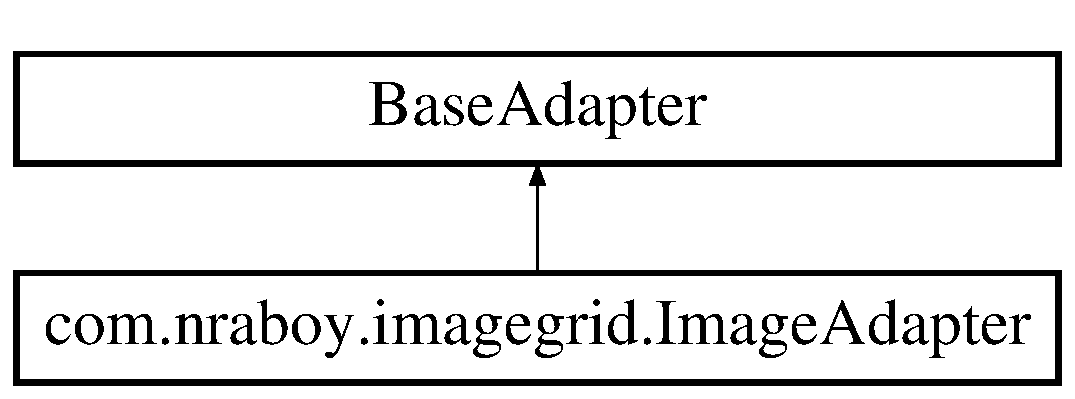
\includegraphics[height=2.000000cm]{classcom_1_1nraboy_1_1imagegrid_1_1_image_adapter}
\end{center}
\end{figure}
\subsection*{Public Member Functions}
\begin{DoxyCompactItemize}
\item 
\hypertarget{classcom_1_1nraboy_1_1imagegrid_1_1_image_adapter_a459bfa4faa7820b3d0b1a25ac143f22a}{}{\bfseries Image\+Adapter} (Context c)\label{classcom_1_1nraboy_1_1imagegrid_1_1_image_adapter_a459bfa4faa7820b3d0b1a25ac143f22a}

\item 
\hypertarget{classcom_1_1nraboy_1_1imagegrid_1_1_image_adapter_aea06691d0ecf89acb951901006ee90ab}{}int {\bfseries get\+Count} ()\label{classcom_1_1nraboy_1_1imagegrid_1_1_image_adapter_aea06691d0ecf89acb951901006ee90ab}

\item 
\hypertarget{classcom_1_1nraboy_1_1imagegrid_1_1_image_adapter_a8788d416d5b172b8edba14ad1b7a8f02}{}Object {\bfseries get\+Item} (int position)\label{classcom_1_1nraboy_1_1imagegrid_1_1_image_adapter_a8788d416d5b172b8edba14ad1b7a8f02}

\item 
\hypertarget{classcom_1_1nraboy_1_1imagegrid_1_1_image_adapter_aa1783e94fab80b95f879266a3055c3d5}{}long {\bfseries get\+Item\+Id} (int position)\label{classcom_1_1nraboy_1_1imagegrid_1_1_image_adapter_aa1783e94fab80b95f879266a3055c3d5}

\item 
View \hyperlink{classcom_1_1nraboy_1_1imagegrid_1_1_image_adapter_a69e1a3e0a4f66193b62d47bb877fcda6}{get\+View} (int position, View convert\+View, View\+Group parent)
\begin{DoxyCompactList}\small\item\em create a new Image\+View for each item referenced by the Adapter \end{DoxyCompactList}\end{DoxyCompactItemize}


\subsection{Detailed Description}
Displays certain size of list depending on the size of stored photos. 

\subsection{Member Function Documentation}
\hypertarget{classcom_1_1nraboy_1_1imagegrid_1_1_image_adapter_a69e1a3e0a4f66193b62d47bb877fcda6}{}\index{com\+::nraboy\+::imagegrid\+::\+Image\+Adapter@{com\+::nraboy\+::imagegrid\+::\+Image\+Adapter}!get\+View@{get\+View}}
\index{get\+View@{get\+View}!com\+::nraboy\+::imagegrid\+::\+Image\+Adapter@{com\+::nraboy\+::imagegrid\+::\+Image\+Adapter}}
\subsubsection[{get\+View(int position, View convert\+View, View\+Group parent)}]{\setlength{\rightskip}{0pt plus 5cm}View com.\+nraboy.\+imagegrid.\+Image\+Adapter.\+get\+View (
\begin{DoxyParamCaption}
\item[{int}]{position, }
\item[{View}]{convert\+View, }
\item[{View\+Group}]{parent}
\end{DoxyParamCaption}
)}\label{classcom_1_1nraboy_1_1imagegrid_1_1_image_adapter_a69e1a3e0a4f66193b62d47bb877fcda6}


create a new Image\+View for each item referenced by the Adapter 

if it\textquotesingle{}s not recycled, initialize some attributes 

The documentation for this class was generated from the following file\+:\begin{DoxyCompactItemize}
\item 
C\+:/\+Users/\+Zwretched/.\+Android\+Studio1.\+4/\+Projects/\+Dress\+Me\+\_\+\+Android/\+Dress\+Me/src/main/java/com/nraboy/imagegrid/Image\+Adapter.\+java\end{DoxyCompactItemize}

\hypertarget{classandroid_1_1support_1_1design_1_1_r_1_1integer}{}\section{android.\+support.\+design.\+R.\+integer Class Reference}
\label{classandroid_1_1support_1_1design_1_1_r_1_1integer}\index{android.\+support.\+design.\+R.\+integer@{android.\+support.\+design.\+R.\+integer}}
\subsection*{Static Public Attributes}
\begin{DoxyCompactItemize}
\item 
\hypertarget{classandroid_1_1support_1_1design_1_1_r_1_1integer_ab0c8a771ad2ae3aba6dc8d9823755f3e}{}static final int {\bfseries abc\+\_\+config\+\_\+activity\+Default\+Dur} = 0x7f0a0002\label{classandroid_1_1support_1_1design_1_1_r_1_1integer_ab0c8a771ad2ae3aba6dc8d9823755f3e}

\item 
\hypertarget{classandroid_1_1support_1_1design_1_1_r_1_1integer_a5cc6424d72a443bb45486cf8746b7bc1}{}static final int {\bfseries abc\+\_\+config\+\_\+activity\+Short\+Dur} = 0x7f0a0003\label{classandroid_1_1support_1_1design_1_1_r_1_1integer_a5cc6424d72a443bb45486cf8746b7bc1}

\item 
\hypertarget{classandroid_1_1support_1_1design_1_1_r_1_1integer_a776adf341d96f93e5e66016c2a8b8edb}{}static final int {\bfseries abc\+\_\+max\+\_\+action\+\_\+buttons} = 0x7f0a0000\label{classandroid_1_1support_1_1design_1_1_r_1_1integer_a776adf341d96f93e5e66016c2a8b8edb}

\item 
\hypertarget{classandroid_1_1support_1_1design_1_1_r_1_1integer_a3b9b1c57b76ebfa9f445b3f40ee6f2ad}{}static final int {\bfseries cancel\+\_\+button\+\_\+image\+\_\+alpha} = 0x7f0a0004\label{classandroid_1_1support_1_1design_1_1_r_1_1integer_a3b9b1c57b76ebfa9f445b3f40ee6f2ad}

\item 
\hypertarget{classandroid_1_1support_1_1design_1_1_r_1_1integer_a938a7c8efcde243e2e8cf2089e78f7f0}{}static final int {\bfseries design\+\_\+snackbar\+\_\+text\+\_\+max\+\_\+lines} = 0x7f0a0001\label{classandroid_1_1support_1_1design_1_1_r_1_1integer_a938a7c8efcde243e2e8cf2089e78f7f0}

\item 
\hypertarget{classandroid_1_1support_1_1design_1_1_r_1_1integer_a4b128748dfc77dbedbe2c85115af5a64}{}static final int {\bfseries status\+\_\+bar\+\_\+notification\+\_\+info\+\_\+maxnum} = 0x7f0a0005\label{classandroid_1_1support_1_1design_1_1_r_1_1integer_a4b128748dfc77dbedbe2c85115af5a64}

\end{DoxyCompactItemize}


The documentation for this class was generated from the following file\+:\begin{DoxyCompactItemize}
\item 
C\+:/\+Users/\+Zwretched/.\+Android\+Studio1.\+4/\+Projects/\+Dress\+Me\+\_\+\+Android/\+Dress\+Me/build/generated/source/r/debug/android/support/design/R.\+java\end{DoxyCompactItemize}

\hypertarget{classcheck_1_1test_1_1_r_1_1integer}{}\section{check.\+test.\+R.\+integer Class Reference}
\label{classcheck_1_1test_1_1_r_1_1integer}\index{check.\+test.\+R.\+integer@{check.\+test.\+R.\+integer}}
\subsection*{Static Public Attributes}
\begin{DoxyCompactItemize}
\item 
\hypertarget{classcheck_1_1test_1_1_r_1_1integer_a4496b10ed558f88e571d20c75f7d04cb}{}static final int {\bfseries abc\+\_\+config\+\_\+activity\+Default\+Dur} =0x7f0a0002\label{classcheck_1_1test_1_1_r_1_1integer_a4496b10ed558f88e571d20c75f7d04cb}

\item 
\hypertarget{classcheck_1_1test_1_1_r_1_1integer_ada6f74d19f5bfb1ef99c034e23d4d4e8}{}static final int {\bfseries abc\+\_\+config\+\_\+activity\+Short\+Dur} =0x7f0a0003\label{classcheck_1_1test_1_1_r_1_1integer_ada6f74d19f5bfb1ef99c034e23d4d4e8}

\item 
\hypertarget{classcheck_1_1test_1_1_r_1_1integer_aecdb9fa9573c8ee5c0f7daf202653996}{}static final int {\bfseries abc\+\_\+max\+\_\+action\+\_\+buttons} =0x7f0a0000\label{classcheck_1_1test_1_1_r_1_1integer_aecdb9fa9573c8ee5c0f7daf202653996}

\item 
\hypertarget{classcheck_1_1test_1_1_r_1_1integer_aa0f6fbe724f746edc499cac5b9475dc5}{}static final int {\bfseries cancel\+\_\+button\+\_\+image\+\_\+alpha} =0x7f0a0004\label{classcheck_1_1test_1_1_r_1_1integer_aa0f6fbe724f746edc499cac5b9475dc5}

\item 
\hypertarget{classcheck_1_1test_1_1_r_1_1integer_ab5ac4d5d12619150b978f9bef589163a}{}static final int {\bfseries design\+\_\+snackbar\+\_\+text\+\_\+max\+\_\+lines} =0x7f0a0001\label{classcheck_1_1test_1_1_r_1_1integer_ab5ac4d5d12619150b978f9bef589163a}

\item 
\hypertarget{classcheck_1_1test_1_1_r_1_1integer_ac970cb362a34ce9359ee9ddb69a44883}{}static final int {\bfseries status\+\_\+bar\+\_\+notification\+\_\+info\+\_\+maxnum} =0x7f0a0005\label{classcheck_1_1test_1_1_r_1_1integer_ac970cb362a34ce9359ee9ddb69a44883}

\end{DoxyCompactItemize}


The documentation for this class was generated from the following file\+:\begin{DoxyCompactItemize}
\item 
C\+:/\+Users/\+Zwretched/.\+Android\+Studio1.\+4/\+Projects/\+Dress\+Me\+\_\+\+Android/\+Dress\+Me/build/generated/source/r/debug/check/test/R.\+java\end{DoxyCompactItemize}

\hypertarget{classandroid_1_1support_1_1v7_1_1appcompat_1_1_r_1_1integer}{}\section{android.\+support.\+v7.\+appcompat.\+R.\+integer Class Reference}
\label{classandroid_1_1support_1_1v7_1_1appcompat_1_1_r_1_1integer}\index{android.\+support.\+v7.\+appcompat.\+R.\+integer@{android.\+support.\+v7.\+appcompat.\+R.\+integer}}
\subsection*{Static Public Attributes}
\begin{DoxyCompactItemize}
\item 
\hypertarget{classandroid_1_1support_1_1v7_1_1appcompat_1_1_r_1_1integer_a4fb2e7826a35c40f397f9f14b86a0c7d}{}static final int {\bfseries abc\+\_\+config\+\_\+activity\+Default\+Dur} = 0x7f0a0002\label{classandroid_1_1support_1_1v7_1_1appcompat_1_1_r_1_1integer_a4fb2e7826a35c40f397f9f14b86a0c7d}

\item 
\hypertarget{classandroid_1_1support_1_1v7_1_1appcompat_1_1_r_1_1integer_a6687bb8055a5a731b1429884734c9565}{}static final int {\bfseries abc\+\_\+config\+\_\+activity\+Short\+Dur} = 0x7f0a0003\label{classandroid_1_1support_1_1v7_1_1appcompat_1_1_r_1_1integer_a6687bb8055a5a731b1429884734c9565}

\item 
\hypertarget{classandroid_1_1support_1_1v7_1_1appcompat_1_1_r_1_1integer_ab30eab0a2cb415ca7fd68f2c56b48817}{}static final int {\bfseries abc\+\_\+max\+\_\+action\+\_\+buttons} = 0x7f0a0000\label{classandroid_1_1support_1_1v7_1_1appcompat_1_1_r_1_1integer_ab30eab0a2cb415ca7fd68f2c56b48817}

\item 
\hypertarget{classandroid_1_1support_1_1v7_1_1appcompat_1_1_r_1_1integer_a21ede1655715ffc1421fbd057706bfa8}{}static final int {\bfseries cancel\+\_\+button\+\_\+image\+\_\+alpha} = 0x7f0a0004\label{classandroid_1_1support_1_1v7_1_1appcompat_1_1_r_1_1integer_a21ede1655715ffc1421fbd057706bfa8}

\item 
\hypertarget{classandroid_1_1support_1_1v7_1_1appcompat_1_1_r_1_1integer_a52a3923b3d9ba3b58e218794b30683dc}{}static final int {\bfseries status\+\_\+bar\+\_\+notification\+\_\+info\+\_\+maxnum} = 0x7f0a0005\label{classandroid_1_1support_1_1v7_1_1appcompat_1_1_r_1_1integer_a52a3923b3d9ba3b58e218794b30683dc}

\end{DoxyCompactItemize}


The documentation for this class was generated from the following file\+:\begin{DoxyCompactItemize}
\item 
C\+:/\+Users/\+Zwretched/.\+Android\+Studio1.\+4/\+Projects/\+Dress\+Me\+\_\+\+Android/\+Dress\+Me/build/generated/source/r/debug/android/support/v7/appcompat/R.\+java\end{DoxyCompactItemize}

\hypertarget{classandroid_1_1support_1_1v7_1_1appcompat_1_1_r_1_1layout}{}\section{android.\+support.\+v7.\+appcompat.\+R.\+layout Class Reference}
\label{classandroid_1_1support_1_1v7_1_1appcompat_1_1_r_1_1layout}\index{android.\+support.\+v7.\+appcompat.\+R.\+layout@{android.\+support.\+v7.\+appcompat.\+R.\+layout}}
\subsection*{Static Public Attributes}
\begin{DoxyCompactItemize}
\item 
\hypertarget{classandroid_1_1support_1_1v7_1_1appcompat_1_1_r_1_1layout_aec65987e63e9073748bd15e578bfe898}{}static final int {\bfseries abc\+\_\+action\+\_\+bar\+\_\+title\+\_\+item} = 0x7f040000\label{classandroid_1_1support_1_1v7_1_1appcompat_1_1_r_1_1layout_aec65987e63e9073748bd15e578bfe898}

\item 
\hypertarget{classandroid_1_1support_1_1v7_1_1appcompat_1_1_r_1_1layout_aef35fa753f14bda2de42d62e894d5d48}{}static final int {\bfseries abc\+\_\+action\+\_\+bar\+\_\+up\+\_\+container} = 0x7f040001\label{classandroid_1_1support_1_1v7_1_1appcompat_1_1_r_1_1layout_aef35fa753f14bda2de42d62e894d5d48}

\item 
\hypertarget{classandroid_1_1support_1_1v7_1_1appcompat_1_1_r_1_1layout_ab2b3d6d1212d6aa5d21fd8d51a445bdd}{}static final int {\bfseries abc\+\_\+action\+\_\+bar\+\_\+view\+\_\+list\+\_\+nav\+\_\+layout} = 0x7f040002\label{classandroid_1_1support_1_1v7_1_1appcompat_1_1_r_1_1layout_ab2b3d6d1212d6aa5d21fd8d51a445bdd}

\item 
\hypertarget{classandroid_1_1support_1_1v7_1_1appcompat_1_1_r_1_1layout_a90577c306263ff0ba660407c3bb14473}{}static final int {\bfseries abc\+\_\+action\+\_\+menu\+\_\+item\+\_\+layout} = 0x7f040003\label{classandroid_1_1support_1_1v7_1_1appcompat_1_1_r_1_1layout_a90577c306263ff0ba660407c3bb14473}

\item 
\hypertarget{classandroid_1_1support_1_1v7_1_1appcompat_1_1_r_1_1layout_ae15076d5fd1b165883c87e6283dde5f9}{}static final int {\bfseries abc\+\_\+action\+\_\+menu\+\_\+layout} = 0x7f040004\label{classandroid_1_1support_1_1v7_1_1appcompat_1_1_r_1_1layout_ae15076d5fd1b165883c87e6283dde5f9}

\item 
\hypertarget{classandroid_1_1support_1_1v7_1_1appcompat_1_1_r_1_1layout_aec4f9e9f9a05a5ca2232a456cb5a6138}{}static final int {\bfseries abc\+\_\+action\+\_\+mode\+\_\+bar} = 0x7f040005\label{classandroid_1_1support_1_1v7_1_1appcompat_1_1_r_1_1layout_aec4f9e9f9a05a5ca2232a456cb5a6138}

\item 
\hypertarget{classandroid_1_1support_1_1v7_1_1appcompat_1_1_r_1_1layout_a5ca5842a7ac8daaf24b3ac54dddca7ac}{}static final int {\bfseries abc\+\_\+action\+\_\+mode\+\_\+close\+\_\+item\+\_\+material} = 0x7f040006\label{classandroid_1_1support_1_1v7_1_1appcompat_1_1_r_1_1layout_a5ca5842a7ac8daaf24b3ac54dddca7ac}

\item 
\hypertarget{classandroid_1_1support_1_1v7_1_1appcompat_1_1_r_1_1layout_aee776be71fc6f95ebb7fc202d1653d33}{}static final int {\bfseries abc\+\_\+activity\+\_\+chooser\+\_\+view} = 0x7f040007\label{classandroid_1_1support_1_1v7_1_1appcompat_1_1_r_1_1layout_aee776be71fc6f95ebb7fc202d1653d33}

\item 
\hypertarget{classandroid_1_1support_1_1v7_1_1appcompat_1_1_r_1_1layout_ac10665103daed966ab8508cf99909639}{}static final int {\bfseries abc\+\_\+activity\+\_\+chooser\+\_\+view\+\_\+list\+\_\+item} = 0x7f040008\label{classandroid_1_1support_1_1v7_1_1appcompat_1_1_r_1_1layout_ac10665103daed966ab8508cf99909639}

\item 
\hypertarget{classandroid_1_1support_1_1v7_1_1appcompat_1_1_r_1_1layout_ad53166dc6778d14218c6ca8d20e4e365}{}static final int {\bfseries abc\+\_\+alert\+\_\+dialog\+\_\+material} = 0x7f040009\label{classandroid_1_1support_1_1v7_1_1appcompat_1_1_r_1_1layout_ad53166dc6778d14218c6ca8d20e4e365}

\item 
\hypertarget{classandroid_1_1support_1_1v7_1_1appcompat_1_1_r_1_1layout_a12b7ab27647b0bb6ed58cf9504524932}{}static final int {\bfseries abc\+\_\+dialog\+\_\+title\+\_\+material} = 0x7f04000a\label{classandroid_1_1support_1_1v7_1_1appcompat_1_1_r_1_1layout_a12b7ab27647b0bb6ed58cf9504524932}

\item 
\hypertarget{classandroid_1_1support_1_1v7_1_1appcompat_1_1_r_1_1layout_a740ce0b38776f4d29c2e8813885ceb2e}{}static final int {\bfseries abc\+\_\+expanded\+\_\+menu\+\_\+layout} = 0x7f04000b\label{classandroid_1_1support_1_1v7_1_1appcompat_1_1_r_1_1layout_a740ce0b38776f4d29c2e8813885ceb2e}

\item 
\hypertarget{classandroid_1_1support_1_1v7_1_1appcompat_1_1_r_1_1layout_a64416b615ad7fe019debb1562106f22b}{}static final int {\bfseries abc\+\_\+list\+\_\+menu\+\_\+item\+\_\+checkbox} = 0x7f04000c\label{classandroid_1_1support_1_1v7_1_1appcompat_1_1_r_1_1layout_a64416b615ad7fe019debb1562106f22b}

\item 
\hypertarget{classandroid_1_1support_1_1v7_1_1appcompat_1_1_r_1_1layout_a11266cae66dfb288775101ecda236866}{}static final int {\bfseries abc\+\_\+list\+\_\+menu\+\_\+item\+\_\+icon} = 0x7f04000d\label{classandroid_1_1support_1_1v7_1_1appcompat_1_1_r_1_1layout_a11266cae66dfb288775101ecda236866}

\item 
\hypertarget{classandroid_1_1support_1_1v7_1_1appcompat_1_1_r_1_1layout_aa5974647c5ae724bcf3b6054fcb11427}{}static final int {\bfseries abc\+\_\+list\+\_\+menu\+\_\+item\+\_\+layout} = 0x7f04000e\label{classandroid_1_1support_1_1v7_1_1appcompat_1_1_r_1_1layout_aa5974647c5ae724bcf3b6054fcb11427}

\item 
\hypertarget{classandroid_1_1support_1_1v7_1_1appcompat_1_1_r_1_1layout_aba244980abc5dc6fe243c8f46131de84}{}static final int {\bfseries abc\+\_\+list\+\_\+menu\+\_\+item\+\_\+radio} = 0x7f04000f\label{classandroid_1_1support_1_1v7_1_1appcompat_1_1_r_1_1layout_aba244980abc5dc6fe243c8f46131de84}

\item 
\hypertarget{classandroid_1_1support_1_1v7_1_1appcompat_1_1_r_1_1layout_ac9b2ae8449ac46de21fed2f9864afbc3}{}static final int {\bfseries abc\+\_\+popup\+\_\+menu\+\_\+item\+\_\+layout} = 0x7f040010\label{classandroid_1_1support_1_1v7_1_1appcompat_1_1_r_1_1layout_ac9b2ae8449ac46de21fed2f9864afbc3}

\item 
\hypertarget{classandroid_1_1support_1_1v7_1_1appcompat_1_1_r_1_1layout_a1193e05438a3988d8cebb0a4810fabc1}{}static final int {\bfseries abc\+\_\+screen\+\_\+content\+\_\+include} = 0x7f040011\label{classandroid_1_1support_1_1v7_1_1appcompat_1_1_r_1_1layout_a1193e05438a3988d8cebb0a4810fabc1}

\item 
\hypertarget{classandroid_1_1support_1_1v7_1_1appcompat_1_1_r_1_1layout_a46cabee4c1c1c293c63a99e850973847}{}static final int {\bfseries abc\+\_\+screen\+\_\+simple} = 0x7f040012\label{classandroid_1_1support_1_1v7_1_1appcompat_1_1_r_1_1layout_a46cabee4c1c1c293c63a99e850973847}

\item 
\hypertarget{classandroid_1_1support_1_1v7_1_1appcompat_1_1_r_1_1layout_acc248e0178ddf81d8ec0eb5056424a5d}{}static final int {\bfseries abc\+\_\+screen\+\_\+simple\+\_\+overlay\+\_\+action\+\_\+mode} = 0x7f040013\label{classandroid_1_1support_1_1v7_1_1appcompat_1_1_r_1_1layout_acc248e0178ddf81d8ec0eb5056424a5d}

\item 
\hypertarget{classandroid_1_1support_1_1v7_1_1appcompat_1_1_r_1_1layout_addd57f53331cb1ff5fd2c53e61bf2805}{}static final int {\bfseries abc\+\_\+screen\+\_\+toolbar} = 0x7f040014\label{classandroid_1_1support_1_1v7_1_1appcompat_1_1_r_1_1layout_addd57f53331cb1ff5fd2c53e61bf2805}

\item 
\hypertarget{classandroid_1_1support_1_1v7_1_1appcompat_1_1_r_1_1layout_a43434db42002b5872fd031eaaea46488}{}static final int {\bfseries abc\+\_\+search\+\_\+dropdown\+\_\+item\+\_\+icons\+\_\+2line} = 0x7f040015\label{classandroid_1_1support_1_1v7_1_1appcompat_1_1_r_1_1layout_a43434db42002b5872fd031eaaea46488}

\item 
\hypertarget{classandroid_1_1support_1_1v7_1_1appcompat_1_1_r_1_1layout_a424314fba766e6fc9c6e6b71ccc00fff}{}static final int {\bfseries abc\+\_\+search\+\_\+view} = 0x7f040016\label{classandroid_1_1support_1_1v7_1_1appcompat_1_1_r_1_1layout_a424314fba766e6fc9c6e6b71ccc00fff}

\item 
\hypertarget{classandroid_1_1support_1_1v7_1_1appcompat_1_1_r_1_1layout_a1f6651d158db2337019984ab97f60e22}{}static final int {\bfseries abc\+\_\+select\+\_\+dialog\+\_\+material} = 0x7f040017\label{classandroid_1_1support_1_1v7_1_1appcompat_1_1_r_1_1layout_a1f6651d158db2337019984ab97f60e22}

\item 
\hypertarget{classandroid_1_1support_1_1v7_1_1appcompat_1_1_r_1_1layout_a07b16aa60214e640ee520c3949ca8ebf}{}static final int {\bfseries notification\+\_\+media\+\_\+action} = 0x7f04002b\label{classandroid_1_1support_1_1v7_1_1appcompat_1_1_r_1_1layout_a07b16aa60214e640ee520c3949ca8ebf}

\item 
\hypertarget{classandroid_1_1support_1_1v7_1_1appcompat_1_1_r_1_1layout_a4942be2a18b0c69205d2f039f4cfb25d}{}static final int {\bfseries notification\+\_\+media\+\_\+cancel\+\_\+action} = 0x7f04002c\label{classandroid_1_1support_1_1v7_1_1appcompat_1_1_r_1_1layout_a4942be2a18b0c69205d2f039f4cfb25d}

\item 
\hypertarget{classandroid_1_1support_1_1v7_1_1appcompat_1_1_r_1_1layout_abc3d68ba9164e5339eb30ac8d1fcc032}{}static final int {\bfseries notification\+\_\+template\+\_\+big\+\_\+media} = 0x7f04002d\label{classandroid_1_1support_1_1v7_1_1appcompat_1_1_r_1_1layout_abc3d68ba9164e5339eb30ac8d1fcc032}

\item 
\hypertarget{classandroid_1_1support_1_1v7_1_1appcompat_1_1_r_1_1layout_adb6b83ae65b94247d0c806e75af83190}{}static final int {\bfseries notification\+\_\+template\+\_\+big\+\_\+media\+\_\+narrow} = 0x7f04002e\label{classandroid_1_1support_1_1v7_1_1appcompat_1_1_r_1_1layout_adb6b83ae65b94247d0c806e75af83190}

\item 
\hypertarget{classandroid_1_1support_1_1v7_1_1appcompat_1_1_r_1_1layout_ac39979905cd11fc790ab4ff2498965bc}{}static final int {\bfseries notification\+\_\+template\+\_\+lines} = 0x7f04002f\label{classandroid_1_1support_1_1v7_1_1appcompat_1_1_r_1_1layout_ac39979905cd11fc790ab4ff2498965bc}

\item 
\hypertarget{classandroid_1_1support_1_1v7_1_1appcompat_1_1_r_1_1layout_a61744f22e936099b070df0771b4b1fee}{}static final int {\bfseries notification\+\_\+template\+\_\+media} = 0x7f040030\label{classandroid_1_1support_1_1v7_1_1appcompat_1_1_r_1_1layout_a61744f22e936099b070df0771b4b1fee}

\item 
\hypertarget{classandroid_1_1support_1_1v7_1_1appcompat_1_1_r_1_1layout_a40ec1f0c58d5ef14dcdabd2917b39098}{}static final int {\bfseries notification\+\_\+template\+\_\+part\+\_\+chronometer} = 0x7f040031\label{classandroid_1_1support_1_1v7_1_1appcompat_1_1_r_1_1layout_a40ec1f0c58d5ef14dcdabd2917b39098}

\item 
\hypertarget{classandroid_1_1support_1_1v7_1_1appcompat_1_1_r_1_1layout_a45b077fa0a865191a582090d784b1163}{}static final int {\bfseries notification\+\_\+template\+\_\+part\+\_\+time} = 0x7f040032\label{classandroid_1_1support_1_1v7_1_1appcompat_1_1_r_1_1layout_a45b077fa0a865191a582090d784b1163}

\item 
\hypertarget{classandroid_1_1support_1_1v7_1_1appcompat_1_1_r_1_1layout_ac19040d9099a5f9d5427814ac4a16e37}{}static final int {\bfseries select\+\_\+dialog\+\_\+item\+\_\+material} = 0x7f040033\label{classandroid_1_1support_1_1v7_1_1appcompat_1_1_r_1_1layout_ac19040d9099a5f9d5427814ac4a16e37}

\item 
\hypertarget{classandroid_1_1support_1_1v7_1_1appcompat_1_1_r_1_1layout_adaf8230a8b0f528256d97c8817a7ea3c}{}static final int {\bfseries select\+\_\+dialog\+\_\+multichoice\+\_\+material} = 0x7f040034\label{classandroid_1_1support_1_1v7_1_1appcompat_1_1_r_1_1layout_adaf8230a8b0f528256d97c8817a7ea3c}

\item 
\hypertarget{classandroid_1_1support_1_1v7_1_1appcompat_1_1_r_1_1layout_a5310ca432c171907a158a12388549c4b}{}static final int {\bfseries select\+\_\+dialog\+\_\+singlechoice\+\_\+material} = 0x7f040035\label{classandroid_1_1support_1_1v7_1_1appcompat_1_1_r_1_1layout_a5310ca432c171907a158a12388549c4b}

\item 
\hypertarget{classandroid_1_1support_1_1v7_1_1appcompat_1_1_r_1_1layout_ad5f037f06366e908921922a2df0a8133}{}static final int {\bfseries support\+\_\+simple\+\_\+spinner\+\_\+dropdown\+\_\+item} = 0x7f040036\label{classandroid_1_1support_1_1v7_1_1appcompat_1_1_r_1_1layout_ad5f037f06366e908921922a2df0a8133}

\end{DoxyCompactItemize}


The documentation for this class was generated from the following file\+:\begin{DoxyCompactItemize}
\item 
C\+:/\+Users/\+Zwretched/.\+Android\+Studio1.\+4/\+Projects/\+Dress\+Me\+\_\+\+Android/\+Dress\+Me/build/generated/source/r/debug/android/support/v7/appcompat/R.\+java\end{DoxyCompactItemize}

\hypertarget{classcheck_1_1test_1_1_r_1_1layout}{}\section{check.\+test.\+R.\+layout Class Reference}
\label{classcheck_1_1test_1_1_r_1_1layout}\index{check.\+test.\+R.\+layout@{check.\+test.\+R.\+layout}}
\subsection*{Static Public Attributes}
\begin{DoxyCompactItemize}
\item 
\hypertarget{classcheck_1_1test_1_1_r_1_1layout_a8ec106402a43e17b70212e29cc51c9d5}{}static final int {\bfseries abc\+\_\+action\+\_\+bar\+\_\+title\+\_\+item} =0x7f040000\label{classcheck_1_1test_1_1_r_1_1layout_a8ec106402a43e17b70212e29cc51c9d5}

\item 
\hypertarget{classcheck_1_1test_1_1_r_1_1layout_aa35c6f8d6fbecb81ebce7267a5481410}{}static final int {\bfseries abc\+\_\+action\+\_\+bar\+\_\+up\+\_\+container} =0x7f040001\label{classcheck_1_1test_1_1_r_1_1layout_aa35c6f8d6fbecb81ebce7267a5481410}

\item 
\hypertarget{classcheck_1_1test_1_1_r_1_1layout_a5e540168f3fd0475fec521ca553e95c8}{}static final int {\bfseries abc\+\_\+action\+\_\+bar\+\_\+view\+\_\+list\+\_\+nav\+\_\+layout} =0x7f040002\label{classcheck_1_1test_1_1_r_1_1layout_a5e540168f3fd0475fec521ca553e95c8}

\item 
\hypertarget{classcheck_1_1test_1_1_r_1_1layout_abcbc47e8059f868d64f8d14c174eebcb}{}static final int {\bfseries abc\+\_\+action\+\_\+menu\+\_\+item\+\_\+layout} =0x7f040003\label{classcheck_1_1test_1_1_r_1_1layout_abcbc47e8059f868d64f8d14c174eebcb}

\item 
\hypertarget{classcheck_1_1test_1_1_r_1_1layout_ac6e2b705494569aec50b1a2eb2003b48}{}static final int {\bfseries abc\+\_\+action\+\_\+menu\+\_\+layout} =0x7f040004\label{classcheck_1_1test_1_1_r_1_1layout_ac6e2b705494569aec50b1a2eb2003b48}

\item 
\hypertarget{classcheck_1_1test_1_1_r_1_1layout_ae3bc1c44f5b31011ba917c940a6aaa81}{}static final int {\bfseries abc\+\_\+action\+\_\+mode\+\_\+bar} =0x7f040005\label{classcheck_1_1test_1_1_r_1_1layout_ae3bc1c44f5b31011ba917c940a6aaa81}

\item 
\hypertarget{classcheck_1_1test_1_1_r_1_1layout_afa4cd09b51ea57d16c73125225864cc5}{}static final int {\bfseries abc\+\_\+action\+\_\+mode\+\_\+close\+\_\+item\+\_\+material} =0x7f040006\label{classcheck_1_1test_1_1_r_1_1layout_afa4cd09b51ea57d16c73125225864cc5}

\item 
\hypertarget{classcheck_1_1test_1_1_r_1_1layout_a43f01e991353d1e199dd375790e879e3}{}static final int {\bfseries abc\+\_\+activity\+\_\+chooser\+\_\+view} =0x7f040007\label{classcheck_1_1test_1_1_r_1_1layout_a43f01e991353d1e199dd375790e879e3}

\item 
\hypertarget{classcheck_1_1test_1_1_r_1_1layout_a78d5e907ed173bcf4c309852e974c8b0}{}static final int {\bfseries abc\+\_\+activity\+\_\+chooser\+\_\+view\+\_\+list\+\_\+item} =0x7f040008\label{classcheck_1_1test_1_1_r_1_1layout_a78d5e907ed173bcf4c309852e974c8b0}

\item 
\hypertarget{classcheck_1_1test_1_1_r_1_1layout_ad3ec5f861c63301c6f5b30a65f3cf81a}{}static final int {\bfseries abc\+\_\+alert\+\_\+dialog\+\_\+material} =0x7f040009\label{classcheck_1_1test_1_1_r_1_1layout_ad3ec5f861c63301c6f5b30a65f3cf81a}

\item 
\hypertarget{classcheck_1_1test_1_1_r_1_1layout_a5cd25f0b0f02d85dfb04aa8f84d575cb}{}static final int {\bfseries abc\+\_\+dialog\+\_\+title\+\_\+material} =0x7f04000a\label{classcheck_1_1test_1_1_r_1_1layout_a5cd25f0b0f02d85dfb04aa8f84d575cb}

\item 
\hypertarget{classcheck_1_1test_1_1_r_1_1layout_a80a19b28516870f09b675587076a9003}{}static final int {\bfseries abc\+\_\+expanded\+\_\+menu\+\_\+layout} =0x7f04000b\label{classcheck_1_1test_1_1_r_1_1layout_a80a19b28516870f09b675587076a9003}

\item 
\hypertarget{classcheck_1_1test_1_1_r_1_1layout_aec12733db72494ce85854d5f76a709fd}{}static final int {\bfseries abc\+\_\+list\+\_\+menu\+\_\+item\+\_\+checkbox} =0x7f04000c\label{classcheck_1_1test_1_1_r_1_1layout_aec12733db72494ce85854d5f76a709fd}

\item 
\hypertarget{classcheck_1_1test_1_1_r_1_1layout_a515e5f1f31d1825d210499eb2e592c8c}{}static final int {\bfseries abc\+\_\+list\+\_\+menu\+\_\+item\+\_\+icon} =0x7f04000d\label{classcheck_1_1test_1_1_r_1_1layout_a515e5f1f31d1825d210499eb2e592c8c}

\item 
\hypertarget{classcheck_1_1test_1_1_r_1_1layout_a81d4330e48d2b8423d60ed67df254f8a}{}static final int {\bfseries abc\+\_\+list\+\_\+menu\+\_\+item\+\_\+layout} =0x7f04000e\label{classcheck_1_1test_1_1_r_1_1layout_a81d4330e48d2b8423d60ed67df254f8a}

\item 
\hypertarget{classcheck_1_1test_1_1_r_1_1layout_a99f6231629ea8add89c64528ff568b15}{}static final int {\bfseries abc\+\_\+list\+\_\+menu\+\_\+item\+\_\+radio} =0x7f04000f\label{classcheck_1_1test_1_1_r_1_1layout_a99f6231629ea8add89c64528ff568b15}

\item 
\hypertarget{classcheck_1_1test_1_1_r_1_1layout_a9b6e405395c9478a75ed824f078b9683}{}static final int {\bfseries abc\+\_\+popup\+\_\+menu\+\_\+item\+\_\+layout} =0x7f040010\label{classcheck_1_1test_1_1_r_1_1layout_a9b6e405395c9478a75ed824f078b9683}

\item 
\hypertarget{classcheck_1_1test_1_1_r_1_1layout_a968b8b84f99b16aaa1cf6658da3dfc54}{}static final int {\bfseries abc\+\_\+screen\+\_\+content\+\_\+include} =0x7f040011\label{classcheck_1_1test_1_1_r_1_1layout_a968b8b84f99b16aaa1cf6658da3dfc54}

\item 
\hypertarget{classcheck_1_1test_1_1_r_1_1layout_abc88d91c1b1754fde66818f940268eca}{}static final int {\bfseries abc\+\_\+screen\+\_\+simple} =0x7f040012\label{classcheck_1_1test_1_1_r_1_1layout_abc88d91c1b1754fde66818f940268eca}

\item 
\hypertarget{classcheck_1_1test_1_1_r_1_1layout_a62b5fa2c61ac07e83b36ee864ec08ab8}{}static final int {\bfseries abc\+\_\+screen\+\_\+simple\+\_\+overlay\+\_\+action\+\_\+mode} =0x7f040013\label{classcheck_1_1test_1_1_r_1_1layout_a62b5fa2c61ac07e83b36ee864ec08ab8}

\item 
\hypertarget{classcheck_1_1test_1_1_r_1_1layout_a068e6eee8182305fb8588f22c7022e43}{}static final int {\bfseries abc\+\_\+screen\+\_\+toolbar} =0x7f040014\label{classcheck_1_1test_1_1_r_1_1layout_a068e6eee8182305fb8588f22c7022e43}

\item 
\hypertarget{classcheck_1_1test_1_1_r_1_1layout_aa8a06790498d3bc43fa197603040a7aa}{}static final int {\bfseries abc\+\_\+search\+\_\+dropdown\+\_\+item\+\_\+icons\+\_\+2line} =0x7f040015\label{classcheck_1_1test_1_1_r_1_1layout_aa8a06790498d3bc43fa197603040a7aa}

\item 
\hypertarget{classcheck_1_1test_1_1_r_1_1layout_ae3f61b1ac3c1d29e959894d24f917deb}{}static final int {\bfseries abc\+\_\+search\+\_\+view} =0x7f040016\label{classcheck_1_1test_1_1_r_1_1layout_ae3f61b1ac3c1d29e959894d24f917deb}

\item 
\hypertarget{classcheck_1_1test_1_1_r_1_1layout_a8ff2283cb2a803cefe607c9e9276b728}{}static final int {\bfseries abc\+\_\+select\+\_\+dialog\+\_\+material} =0x7f040017\label{classcheck_1_1test_1_1_r_1_1layout_a8ff2283cb2a803cefe607c9e9276b728}

\item 
\hypertarget{classcheck_1_1test_1_1_r_1_1layout_a063d7f23adcc86ea7ffd68a40e1d70b1}{}static final int {\bfseries activity\+\_\+creation\+\_\+screen} =0x7f040018\label{classcheck_1_1test_1_1_r_1_1layout_a063d7f23adcc86ea7ffd68a40e1d70b1}

\item 
\hypertarget{classcheck_1_1test_1_1_r_1_1layout_a44096e72a2527e673d9605c949cc73cd}{}static final int {\bfseries activity\+\_\+favorites} =0x7f040019\label{classcheck_1_1test_1_1_r_1_1layout_a44096e72a2527e673d9605c949cc73cd}

\item 
\hypertarget{classcheck_1_1test_1_1_r_1_1layout_a8de1b0f1db4292417ee244412dd3e25a}{}static final int {\bfseries activity\+\_\+main} =0x7f04001a\label{classcheck_1_1test_1_1_r_1_1layout_a8de1b0f1db4292417ee244412dd3e25a}

\item 
\hypertarget{classcheck_1_1test_1_1_r_1_1layout_a6d68bef2b3e77db82615cb93adcaf84d}{}static final int {\bfseries activity\+\_\+main2} =0x7f04001b\label{classcheck_1_1test_1_1_r_1_1layout_a6d68bef2b3e77db82615cb93adcaf84d}

\item 
\hypertarget{classcheck_1_1test_1_1_r_1_1layout_a09803b49bc3914e3115aa4d189acfdfc}{}static final int {\bfseries content\+\_\+creation\+\_\+screen} =0x7f04001c\label{classcheck_1_1test_1_1_r_1_1layout_a09803b49bc3914e3115aa4d189acfdfc}

\item 
\hypertarget{classcheck_1_1test_1_1_r_1_1layout_a06c29b2f98cf4011a46f5385b544e9d2}{}static final int {\bfseries content\+\_\+favorites} =0x7f04001d\label{classcheck_1_1test_1_1_r_1_1layout_a06c29b2f98cf4011a46f5385b544e9d2}

\item 
\hypertarget{classcheck_1_1test_1_1_r_1_1layout_a8baea0d5d5ed352fbf8a5f7b907906d7}{}static final int {\bfseries content\+\_\+main} =0x7f04001e\label{classcheck_1_1test_1_1_r_1_1layout_a8baea0d5d5ed352fbf8a5f7b907906d7}

\item 
\hypertarget{classcheck_1_1test_1_1_r_1_1layout_a7434aff5e01aebb5fa49fbfcb0ace097}{}static final int {\bfseries content\+\_\+main2} =0x7f04001f\label{classcheck_1_1test_1_1_r_1_1layout_a7434aff5e01aebb5fa49fbfcb0ace097}

\item 
\hypertarget{classcheck_1_1test_1_1_r_1_1layout_ac16096d23a0078227f092b1c1808567b}{}static final int {\bfseries design\+\_\+layout\+\_\+snackbar} =0x7f040020\label{classcheck_1_1test_1_1_r_1_1layout_ac16096d23a0078227f092b1c1808567b}

\item 
\hypertarget{classcheck_1_1test_1_1_r_1_1layout_a7a05fb8021d9aff9737b056ec1b4da27}{}static final int {\bfseries design\+\_\+layout\+\_\+snackbar\+\_\+include} =0x7f040021\label{classcheck_1_1test_1_1_r_1_1layout_a7a05fb8021d9aff9737b056ec1b4da27}

\item 
\hypertarget{classcheck_1_1test_1_1_r_1_1layout_a8b4eb6e8ed8cc4696426890aed9fd7c8}{}static final int {\bfseries design\+\_\+layout\+\_\+tab\+\_\+icon} =0x7f040022\label{classcheck_1_1test_1_1_r_1_1layout_a8b4eb6e8ed8cc4696426890aed9fd7c8}

\item 
\hypertarget{classcheck_1_1test_1_1_r_1_1layout_ad11e6ae357ff64af9d552a9afd274743}{}static final int {\bfseries design\+\_\+layout\+\_\+tab\+\_\+text} =0x7f040023\label{classcheck_1_1test_1_1_r_1_1layout_ad11e6ae357ff64af9d552a9afd274743}

\item 
\hypertarget{classcheck_1_1test_1_1_r_1_1layout_ac28002e55577f34056c50c24da1814ac}{}static final int {\bfseries design\+\_\+navigation\+\_\+item} =0x7f040024\label{classcheck_1_1test_1_1_r_1_1layout_ac28002e55577f34056c50c24da1814ac}

\item 
\hypertarget{classcheck_1_1test_1_1_r_1_1layout_a0cf8ff3dc3f4576c03077c1c8efb1ce3}{}static final int {\bfseries design\+\_\+navigation\+\_\+item\+\_\+header} =0x7f040025\label{classcheck_1_1test_1_1_r_1_1layout_a0cf8ff3dc3f4576c03077c1c8efb1ce3}

\item 
\hypertarget{classcheck_1_1test_1_1_r_1_1layout_aa77e03054476a59cdae34249adfd8219}{}static final int {\bfseries design\+\_\+navigation\+\_\+item\+\_\+separator} =0x7f040026\label{classcheck_1_1test_1_1_r_1_1layout_aa77e03054476a59cdae34249adfd8219}

\item 
\hypertarget{classcheck_1_1test_1_1_r_1_1layout_ad56c699600b2bbf7a268151c753dfd4d}{}static final int {\bfseries design\+\_\+navigation\+\_\+item\+\_\+subheader} =0x7f040027\label{classcheck_1_1test_1_1_r_1_1layout_ad56c699600b2bbf7a268151c753dfd4d}

\item 
\hypertarget{classcheck_1_1test_1_1_r_1_1layout_a26d5579b82f2e956b80fc225e9003764}{}static final int {\bfseries design\+\_\+navigation\+\_\+menu} =0x7f040028\label{classcheck_1_1test_1_1_r_1_1layout_a26d5579b82f2e956b80fc225e9003764}

\item 
\hypertarget{classcheck_1_1test_1_1_r_1_1layout_a936f090e87e303f1a37ecf9801722a43}{}static final int {\bfseries list\+\_\+item} =0x7f040029\label{classcheck_1_1test_1_1_r_1_1layout_a936f090e87e303f1a37ecf9801722a43}

\item 
\hypertarget{classcheck_1_1test_1_1_r_1_1layout_a0ea312ebbce4c717f966391b1474d4a8}{}static final int {\bfseries listview\+\_\+manager} =0x7f04002a\label{classcheck_1_1test_1_1_r_1_1layout_a0ea312ebbce4c717f966391b1474d4a8}

\item 
\hypertarget{classcheck_1_1test_1_1_r_1_1layout_a0602ece9384a2ea900e3b397542a2f86}{}static final int {\bfseries notification\+\_\+media\+\_\+action} =0x7f04002b\label{classcheck_1_1test_1_1_r_1_1layout_a0602ece9384a2ea900e3b397542a2f86}

\item 
\hypertarget{classcheck_1_1test_1_1_r_1_1layout_ae91122be0c178752009db64dc2251665}{}static final int {\bfseries notification\+\_\+media\+\_\+cancel\+\_\+action} =0x7f04002c\label{classcheck_1_1test_1_1_r_1_1layout_ae91122be0c178752009db64dc2251665}

\item 
\hypertarget{classcheck_1_1test_1_1_r_1_1layout_a33227181f9b46f240c767cdc0fc7e884}{}static final int {\bfseries notification\+\_\+template\+\_\+big\+\_\+media} =0x7f04002d\label{classcheck_1_1test_1_1_r_1_1layout_a33227181f9b46f240c767cdc0fc7e884}

\item 
\hypertarget{classcheck_1_1test_1_1_r_1_1layout_ac758610a4c899de9186b0c6d7ade6afa}{}static final int {\bfseries notification\+\_\+template\+\_\+big\+\_\+media\+\_\+narrow} =0x7f04002e\label{classcheck_1_1test_1_1_r_1_1layout_ac758610a4c899de9186b0c6d7ade6afa}

\item 
\hypertarget{classcheck_1_1test_1_1_r_1_1layout_a7eda394bf92c369acbf49e2dabc4bdd1}{}static final int {\bfseries notification\+\_\+template\+\_\+lines} =0x7f04002f\label{classcheck_1_1test_1_1_r_1_1layout_a7eda394bf92c369acbf49e2dabc4bdd1}

\item 
\hypertarget{classcheck_1_1test_1_1_r_1_1layout_a4874b98f244a62b99084b3163690a312}{}static final int {\bfseries notification\+\_\+template\+\_\+media} =0x7f040030\label{classcheck_1_1test_1_1_r_1_1layout_a4874b98f244a62b99084b3163690a312}

\item 
\hypertarget{classcheck_1_1test_1_1_r_1_1layout_a759f2a988336210c16ffe449d78698c5}{}static final int {\bfseries notification\+\_\+template\+\_\+part\+\_\+chronometer} =0x7f040031\label{classcheck_1_1test_1_1_r_1_1layout_a759f2a988336210c16ffe449d78698c5}

\item 
\hypertarget{classcheck_1_1test_1_1_r_1_1layout_ae7ab5fcc62d4df0d85d7aaefdaef5245}{}static final int {\bfseries notification\+\_\+template\+\_\+part\+\_\+time} =0x7f040032\label{classcheck_1_1test_1_1_r_1_1layout_ae7ab5fcc62d4df0d85d7aaefdaef5245}

\item 
\hypertarget{classcheck_1_1test_1_1_r_1_1layout_a5c6c9404ee36c4e2838cb49da1246b62}{}static final int {\bfseries select\+\_\+dialog\+\_\+item\+\_\+material} =0x7f040033\label{classcheck_1_1test_1_1_r_1_1layout_a5c6c9404ee36c4e2838cb49da1246b62}

\item 
\hypertarget{classcheck_1_1test_1_1_r_1_1layout_a2706d60cbb9202e99b18bd5da86cd5c0}{}static final int {\bfseries select\+\_\+dialog\+\_\+multichoice\+\_\+material} =0x7f040034\label{classcheck_1_1test_1_1_r_1_1layout_a2706d60cbb9202e99b18bd5da86cd5c0}

\item 
\hypertarget{classcheck_1_1test_1_1_r_1_1layout_aa6e01603ab30ea0c822a5f9ddae3f534}{}static final int {\bfseries select\+\_\+dialog\+\_\+singlechoice\+\_\+material} =0x7f040035\label{classcheck_1_1test_1_1_r_1_1layout_aa6e01603ab30ea0c822a5f9ddae3f534}

\item 
\hypertarget{classcheck_1_1test_1_1_r_1_1layout_a2e4d751b1e5d2c3c166133e5c8fa4060}{}static final int {\bfseries support\+\_\+simple\+\_\+spinner\+\_\+dropdown\+\_\+item} =0x7f040036\label{classcheck_1_1test_1_1_r_1_1layout_a2e4d751b1e5d2c3c166133e5c8fa4060}

\end{DoxyCompactItemize}


The documentation for this class was generated from the following file\+:\begin{DoxyCompactItemize}
\item 
C\+:/\+Users/\+Zwretched/.\+Android\+Studio1.\+4/\+Projects/\+Dress\+Me\+\_\+\+Android/\+Dress\+Me/build/generated/source/r/debug/check/test/R.\+java\end{DoxyCompactItemize}

\hypertarget{classandroid_1_1support_1_1design_1_1_r_1_1layout}{}\section{android.\+support.\+design.\+R.\+layout Class Reference}
\label{classandroid_1_1support_1_1design_1_1_r_1_1layout}\index{android.\+support.\+design.\+R.\+layout@{android.\+support.\+design.\+R.\+layout}}
\subsection*{Static Public Attributes}
\begin{DoxyCompactItemize}
\item 
\hypertarget{classandroid_1_1support_1_1design_1_1_r_1_1layout_a531b33a0bb0538dd1d077ef414f13912}{}static final int {\bfseries abc\+\_\+action\+\_\+bar\+\_\+title\+\_\+item} = 0x7f040000\label{classandroid_1_1support_1_1design_1_1_r_1_1layout_a531b33a0bb0538dd1d077ef414f13912}

\item 
\hypertarget{classandroid_1_1support_1_1design_1_1_r_1_1layout_a65ed125f76e124be64ba517ed6388a2f}{}static final int {\bfseries abc\+\_\+action\+\_\+bar\+\_\+up\+\_\+container} = 0x7f040001\label{classandroid_1_1support_1_1design_1_1_r_1_1layout_a65ed125f76e124be64ba517ed6388a2f}

\item 
\hypertarget{classandroid_1_1support_1_1design_1_1_r_1_1layout_a079dfdfef917e52dcfe6fe5f09bbb311}{}static final int {\bfseries abc\+\_\+action\+\_\+bar\+\_\+view\+\_\+list\+\_\+nav\+\_\+layout} = 0x7f040002\label{classandroid_1_1support_1_1design_1_1_r_1_1layout_a079dfdfef917e52dcfe6fe5f09bbb311}

\item 
\hypertarget{classandroid_1_1support_1_1design_1_1_r_1_1layout_aa31161c408085d6a0ce8b75edb2821bf}{}static final int {\bfseries abc\+\_\+action\+\_\+menu\+\_\+item\+\_\+layout} = 0x7f040003\label{classandroid_1_1support_1_1design_1_1_r_1_1layout_aa31161c408085d6a0ce8b75edb2821bf}

\item 
\hypertarget{classandroid_1_1support_1_1design_1_1_r_1_1layout_a950d7d0ec60597ed0fceff4da4d8a6ee}{}static final int {\bfseries abc\+\_\+action\+\_\+menu\+\_\+layout} = 0x7f040004\label{classandroid_1_1support_1_1design_1_1_r_1_1layout_a950d7d0ec60597ed0fceff4da4d8a6ee}

\item 
\hypertarget{classandroid_1_1support_1_1design_1_1_r_1_1layout_a4ed2ccdae8bbfabdb968a36d217cfb5e}{}static final int {\bfseries abc\+\_\+action\+\_\+mode\+\_\+bar} = 0x7f040005\label{classandroid_1_1support_1_1design_1_1_r_1_1layout_a4ed2ccdae8bbfabdb968a36d217cfb5e}

\item 
\hypertarget{classandroid_1_1support_1_1design_1_1_r_1_1layout_acf611bbfd39d0104f58774f7799a59c0}{}static final int {\bfseries abc\+\_\+action\+\_\+mode\+\_\+close\+\_\+item\+\_\+material} = 0x7f040006\label{classandroid_1_1support_1_1design_1_1_r_1_1layout_acf611bbfd39d0104f58774f7799a59c0}

\item 
\hypertarget{classandroid_1_1support_1_1design_1_1_r_1_1layout_a43a54b73c3cfb776e7a50094cc91b8c1}{}static final int {\bfseries abc\+\_\+activity\+\_\+chooser\+\_\+view} = 0x7f040007\label{classandroid_1_1support_1_1design_1_1_r_1_1layout_a43a54b73c3cfb776e7a50094cc91b8c1}

\item 
\hypertarget{classandroid_1_1support_1_1design_1_1_r_1_1layout_aadf7a74bdcfcc0214b577ca8912b47d1}{}static final int {\bfseries abc\+\_\+activity\+\_\+chooser\+\_\+view\+\_\+list\+\_\+item} = 0x7f040008\label{classandroid_1_1support_1_1design_1_1_r_1_1layout_aadf7a74bdcfcc0214b577ca8912b47d1}

\item 
\hypertarget{classandroid_1_1support_1_1design_1_1_r_1_1layout_ae345cc83bdcd7ddfdbf543e4483b9515}{}static final int {\bfseries abc\+\_\+alert\+\_\+dialog\+\_\+material} = 0x7f040009\label{classandroid_1_1support_1_1design_1_1_r_1_1layout_ae345cc83bdcd7ddfdbf543e4483b9515}

\item 
\hypertarget{classandroid_1_1support_1_1design_1_1_r_1_1layout_ab98202b6d43ce7854889d44c825908af}{}static final int {\bfseries abc\+\_\+dialog\+\_\+title\+\_\+material} = 0x7f04000a\label{classandroid_1_1support_1_1design_1_1_r_1_1layout_ab98202b6d43ce7854889d44c825908af}

\item 
\hypertarget{classandroid_1_1support_1_1design_1_1_r_1_1layout_a8dd1e24e585a6ed15385c5fa7a9a543b}{}static final int {\bfseries abc\+\_\+expanded\+\_\+menu\+\_\+layout} = 0x7f04000b\label{classandroid_1_1support_1_1design_1_1_r_1_1layout_a8dd1e24e585a6ed15385c5fa7a9a543b}

\item 
\hypertarget{classandroid_1_1support_1_1design_1_1_r_1_1layout_a2c90f63e9a8c8b2e68269eae863ae97d}{}static final int {\bfseries abc\+\_\+list\+\_\+menu\+\_\+item\+\_\+checkbox} = 0x7f04000c\label{classandroid_1_1support_1_1design_1_1_r_1_1layout_a2c90f63e9a8c8b2e68269eae863ae97d}

\item 
\hypertarget{classandroid_1_1support_1_1design_1_1_r_1_1layout_aaa44eb526bc60350d6aaf3be20618c64}{}static final int {\bfseries abc\+\_\+list\+\_\+menu\+\_\+item\+\_\+icon} = 0x7f04000d\label{classandroid_1_1support_1_1design_1_1_r_1_1layout_aaa44eb526bc60350d6aaf3be20618c64}

\item 
\hypertarget{classandroid_1_1support_1_1design_1_1_r_1_1layout_a7558278a1602fc132cb8a9c6017b5a09}{}static final int {\bfseries abc\+\_\+list\+\_\+menu\+\_\+item\+\_\+layout} = 0x7f04000e\label{classandroid_1_1support_1_1design_1_1_r_1_1layout_a7558278a1602fc132cb8a9c6017b5a09}

\item 
\hypertarget{classandroid_1_1support_1_1design_1_1_r_1_1layout_abeaea14dea4b8b1164cc05e47ab8dde2}{}static final int {\bfseries abc\+\_\+list\+\_\+menu\+\_\+item\+\_\+radio} = 0x7f04000f\label{classandroid_1_1support_1_1design_1_1_r_1_1layout_abeaea14dea4b8b1164cc05e47ab8dde2}

\item 
\hypertarget{classandroid_1_1support_1_1design_1_1_r_1_1layout_a96f5a59e279f130e091777270663f7a3}{}static final int {\bfseries abc\+\_\+popup\+\_\+menu\+\_\+item\+\_\+layout} = 0x7f040010\label{classandroid_1_1support_1_1design_1_1_r_1_1layout_a96f5a59e279f130e091777270663f7a3}

\item 
\hypertarget{classandroid_1_1support_1_1design_1_1_r_1_1layout_ac1ea0700228284eac706a3d1369d7fab}{}static final int {\bfseries abc\+\_\+screen\+\_\+content\+\_\+include} = 0x7f040011\label{classandroid_1_1support_1_1design_1_1_r_1_1layout_ac1ea0700228284eac706a3d1369d7fab}

\item 
\hypertarget{classandroid_1_1support_1_1design_1_1_r_1_1layout_a957aec20303a776f195a00390496753b}{}static final int {\bfseries abc\+\_\+screen\+\_\+simple} = 0x7f040012\label{classandroid_1_1support_1_1design_1_1_r_1_1layout_a957aec20303a776f195a00390496753b}

\item 
\hypertarget{classandroid_1_1support_1_1design_1_1_r_1_1layout_a3098585a2f723080061fd42dd4d91d94}{}static final int {\bfseries abc\+\_\+screen\+\_\+simple\+\_\+overlay\+\_\+action\+\_\+mode} = 0x7f040013\label{classandroid_1_1support_1_1design_1_1_r_1_1layout_a3098585a2f723080061fd42dd4d91d94}

\item 
\hypertarget{classandroid_1_1support_1_1design_1_1_r_1_1layout_a27b17cd1e50e5101addd868ef7348ead}{}static final int {\bfseries abc\+\_\+screen\+\_\+toolbar} = 0x7f040014\label{classandroid_1_1support_1_1design_1_1_r_1_1layout_a27b17cd1e50e5101addd868ef7348ead}

\item 
\hypertarget{classandroid_1_1support_1_1design_1_1_r_1_1layout_ac425206367179409e7f02a364f820c2f}{}static final int {\bfseries abc\+\_\+search\+\_\+dropdown\+\_\+item\+\_\+icons\+\_\+2line} = 0x7f040015\label{classandroid_1_1support_1_1design_1_1_r_1_1layout_ac425206367179409e7f02a364f820c2f}

\item 
\hypertarget{classandroid_1_1support_1_1design_1_1_r_1_1layout_aaddf023060f3d2bcf6aeaa8a47cba6da}{}static final int {\bfseries abc\+\_\+search\+\_\+view} = 0x7f040016\label{classandroid_1_1support_1_1design_1_1_r_1_1layout_aaddf023060f3d2bcf6aeaa8a47cba6da}

\item 
\hypertarget{classandroid_1_1support_1_1design_1_1_r_1_1layout_a4138a3a5dbeee0c457208d182140fff7}{}static final int {\bfseries abc\+\_\+select\+\_\+dialog\+\_\+material} = 0x7f040017\label{classandroid_1_1support_1_1design_1_1_r_1_1layout_a4138a3a5dbeee0c457208d182140fff7}

\item 
\hypertarget{classandroid_1_1support_1_1design_1_1_r_1_1layout_a8d7f864b1731af8b70ca0654071ad76e}{}static final int {\bfseries design\+\_\+layout\+\_\+snackbar} = 0x7f040020\label{classandroid_1_1support_1_1design_1_1_r_1_1layout_a8d7f864b1731af8b70ca0654071ad76e}

\item 
\hypertarget{classandroid_1_1support_1_1design_1_1_r_1_1layout_a98d09e99d5eb781fb883b7b11df24dd6}{}static final int {\bfseries design\+\_\+layout\+\_\+snackbar\+\_\+include} = 0x7f040021\label{classandroid_1_1support_1_1design_1_1_r_1_1layout_a98d09e99d5eb781fb883b7b11df24dd6}

\item 
\hypertarget{classandroid_1_1support_1_1design_1_1_r_1_1layout_a736d88071f77d19d86aa429d88c05d80}{}static final int {\bfseries design\+\_\+layout\+\_\+tab\+\_\+icon} = 0x7f040022\label{classandroid_1_1support_1_1design_1_1_r_1_1layout_a736d88071f77d19d86aa429d88c05d80}

\item 
\hypertarget{classandroid_1_1support_1_1design_1_1_r_1_1layout_a25a0ff3a8a0971cf70afd38cceec34ee}{}static final int {\bfseries design\+\_\+layout\+\_\+tab\+\_\+text} = 0x7f040023\label{classandroid_1_1support_1_1design_1_1_r_1_1layout_a25a0ff3a8a0971cf70afd38cceec34ee}

\item 
\hypertarget{classandroid_1_1support_1_1design_1_1_r_1_1layout_a6f870feafd3976058e65635845afdf28}{}static final int {\bfseries design\+\_\+navigation\+\_\+item} = 0x7f040024\label{classandroid_1_1support_1_1design_1_1_r_1_1layout_a6f870feafd3976058e65635845afdf28}

\item 
\hypertarget{classandroid_1_1support_1_1design_1_1_r_1_1layout_ad5d1e4411a5d259439aaeb5d66ee87e4}{}static final int {\bfseries design\+\_\+navigation\+\_\+item\+\_\+header} = 0x7f040025\label{classandroid_1_1support_1_1design_1_1_r_1_1layout_ad5d1e4411a5d259439aaeb5d66ee87e4}

\item 
\hypertarget{classandroid_1_1support_1_1design_1_1_r_1_1layout_ad96876f67d154d3fd08794c12c1efc59}{}static final int {\bfseries design\+\_\+navigation\+\_\+item\+\_\+separator} = 0x7f040026\label{classandroid_1_1support_1_1design_1_1_r_1_1layout_ad96876f67d154d3fd08794c12c1efc59}

\item 
\hypertarget{classandroid_1_1support_1_1design_1_1_r_1_1layout_a3d4b46f5c32b100f48b1cf108d0f5b68}{}static final int {\bfseries design\+\_\+navigation\+\_\+item\+\_\+subheader} = 0x7f040027\label{classandroid_1_1support_1_1design_1_1_r_1_1layout_a3d4b46f5c32b100f48b1cf108d0f5b68}

\item 
\hypertarget{classandroid_1_1support_1_1design_1_1_r_1_1layout_a68f5d00d1b2b0dbca3b4c40fcc85bd25}{}static final int {\bfseries design\+\_\+navigation\+\_\+menu} = 0x7f040028\label{classandroid_1_1support_1_1design_1_1_r_1_1layout_a68f5d00d1b2b0dbca3b4c40fcc85bd25}

\item 
\hypertarget{classandroid_1_1support_1_1design_1_1_r_1_1layout_ae4178499ed0a627b4082b09cfae99907}{}static final int {\bfseries notification\+\_\+media\+\_\+action} = 0x7f04002b\label{classandroid_1_1support_1_1design_1_1_r_1_1layout_ae4178499ed0a627b4082b09cfae99907}

\item 
\hypertarget{classandroid_1_1support_1_1design_1_1_r_1_1layout_a2afa4dd43d64918dd43e5c1b6ee43b97}{}static final int {\bfseries notification\+\_\+media\+\_\+cancel\+\_\+action} = 0x7f04002c\label{classandroid_1_1support_1_1design_1_1_r_1_1layout_a2afa4dd43d64918dd43e5c1b6ee43b97}

\item 
\hypertarget{classandroid_1_1support_1_1design_1_1_r_1_1layout_a937801124bdcdd939ce59fe3913a9762}{}static final int {\bfseries notification\+\_\+template\+\_\+big\+\_\+media} = 0x7f04002d\label{classandroid_1_1support_1_1design_1_1_r_1_1layout_a937801124bdcdd939ce59fe3913a9762}

\item 
\hypertarget{classandroid_1_1support_1_1design_1_1_r_1_1layout_a85e748195c9daddc8bb8fe726a1a5da2}{}static final int {\bfseries notification\+\_\+template\+\_\+big\+\_\+media\+\_\+narrow} = 0x7f04002e\label{classandroid_1_1support_1_1design_1_1_r_1_1layout_a85e748195c9daddc8bb8fe726a1a5da2}

\item 
\hypertarget{classandroid_1_1support_1_1design_1_1_r_1_1layout_a3b564781a7a1175a42bafaa390592c97}{}static final int {\bfseries notification\+\_\+template\+\_\+lines} = 0x7f04002f\label{classandroid_1_1support_1_1design_1_1_r_1_1layout_a3b564781a7a1175a42bafaa390592c97}

\item 
\hypertarget{classandroid_1_1support_1_1design_1_1_r_1_1layout_af6499fd4c261801e10b2e023556ceb2e}{}static final int {\bfseries notification\+\_\+template\+\_\+media} = 0x7f040030\label{classandroid_1_1support_1_1design_1_1_r_1_1layout_af6499fd4c261801e10b2e023556ceb2e}

\item 
\hypertarget{classandroid_1_1support_1_1design_1_1_r_1_1layout_adbf595dcbbe5468a640c75da765e94c5}{}static final int {\bfseries notification\+\_\+template\+\_\+part\+\_\+chronometer} = 0x7f040031\label{classandroid_1_1support_1_1design_1_1_r_1_1layout_adbf595dcbbe5468a640c75da765e94c5}

\item 
\hypertarget{classandroid_1_1support_1_1design_1_1_r_1_1layout_a207f018f5184f266fb707b3c42dff303}{}static final int {\bfseries notification\+\_\+template\+\_\+part\+\_\+time} = 0x7f040032\label{classandroid_1_1support_1_1design_1_1_r_1_1layout_a207f018f5184f266fb707b3c42dff303}

\item 
\hypertarget{classandroid_1_1support_1_1design_1_1_r_1_1layout_aab2090fcba37187805603c08746aa8cc}{}static final int {\bfseries select\+\_\+dialog\+\_\+item\+\_\+material} = 0x7f040033\label{classandroid_1_1support_1_1design_1_1_r_1_1layout_aab2090fcba37187805603c08746aa8cc}

\item 
\hypertarget{classandroid_1_1support_1_1design_1_1_r_1_1layout_a3d2eb3f803ab59c599c7022c15479bb8}{}static final int {\bfseries select\+\_\+dialog\+\_\+multichoice\+\_\+material} = 0x7f040034\label{classandroid_1_1support_1_1design_1_1_r_1_1layout_a3d2eb3f803ab59c599c7022c15479bb8}

\item 
\hypertarget{classandroid_1_1support_1_1design_1_1_r_1_1layout_af908cc6a223fbe33d22bb3088dfc11b2}{}static final int {\bfseries select\+\_\+dialog\+\_\+singlechoice\+\_\+material} = 0x7f040035\label{classandroid_1_1support_1_1design_1_1_r_1_1layout_af908cc6a223fbe33d22bb3088dfc11b2}

\item 
\hypertarget{classandroid_1_1support_1_1design_1_1_r_1_1layout_a4de293b6e7223138532dd164026cd9c6}{}static final int {\bfseries support\+\_\+simple\+\_\+spinner\+\_\+dropdown\+\_\+item} = 0x7f040036\label{classandroid_1_1support_1_1design_1_1_r_1_1layout_a4de293b6e7223138532dd164026cd9c6}

\end{DoxyCompactItemize}


The documentation for this class was generated from the following file\+:\begin{DoxyCompactItemize}
\item 
C\+:/\+Users/\+Zwretched/.\+Android\+Studio1.\+4/\+Projects/\+Dress\+Me\+\_\+\+Android/\+Dress\+Me/build/generated/source/r/debug/android/support/design/R.\+java\end{DoxyCompactItemize}

\hypertarget{classcom_1_1nraboy_1_1imagegrid_1_1_main2_activity}{}\section{com.\+nraboy.\+imagegrid.\+Main2\+Activity Class Reference}
\label{classcom_1_1nraboy_1_1imagegrid_1_1_main2_activity}\index{com.\+nraboy.\+imagegrid.\+Main2\+Activity@{com.\+nraboy.\+imagegrid.\+Main2\+Activity}}


Screen for displaying uploaded garments.  


Inheritance diagram for com.\+nraboy.\+imagegrid.\+Main2\+Activity\+:\begin{figure}[H]
\begin{center}
\leavevmode
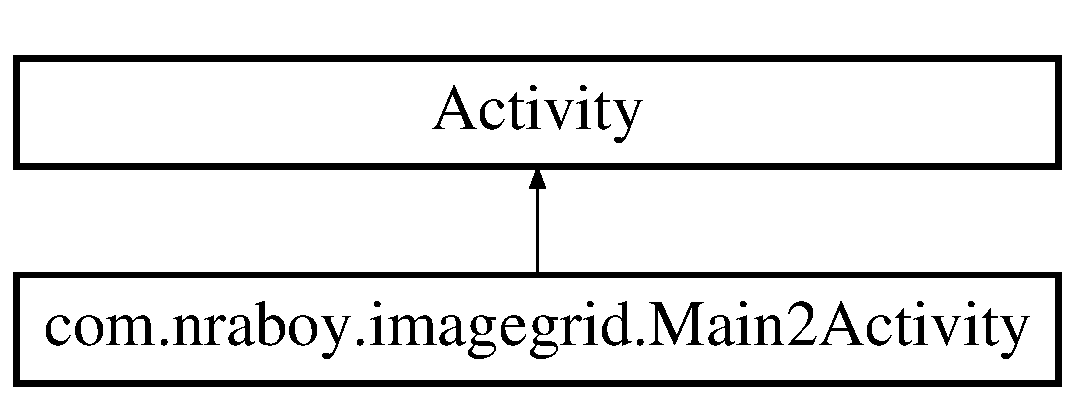
\includegraphics[height=2.000000cm]{classcom_1_1nraboy_1_1imagegrid_1_1_main2_activity}
\end{center}
\end{figure}
\subsection*{Public Member Functions}
\begin{DoxyCompactItemize}
\item 
\hypertarget{classcom_1_1nraboy_1_1imagegrid_1_1_main2_activity_ac783af0f609459727ebf7d3eecc11d2f}{}void {\bfseries on\+Create} (Bundle saved\+Instance\+State)\label{classcom_1_1nraboy_1_1imagegrid_1_1_main2_activity_ac783af0f609459727ebf7d3eecc11d2f}

\end{DoxyCompactItemize}


\subsection{Detailed Description}
Screen for displaying uploaded garments. 

The documentation for this class was generated from the following file\+:\begin{DoxyCompactItemize}
\item 
C\+:/\+Users/\+Zwretched/.\+Android\+Studio1.\+4/\+Projects/\+Dress\+Me\+\_\+\+Android/\+Dress\+Me/src/main/java/com/nraboy/imagegrid/Main2\+Activity.\+java\end{DoxyCompactItemize}

\hypertarget{classcheck_1_1test_1_1_main_activity}{}\section{check.\+test.\+Main\+Activity Class Reference}
\label{classcheck_1_1test_1_1_main_activity}\index{check.\+test.\+Main\+Activity@{check.\+test.\+Main\+Activity}}


First Application Page.  


Inheritance diagram for check.\+test.\+Main\+Activity\+:\begin{figure}[H]
\begin{center}
\leavevmode
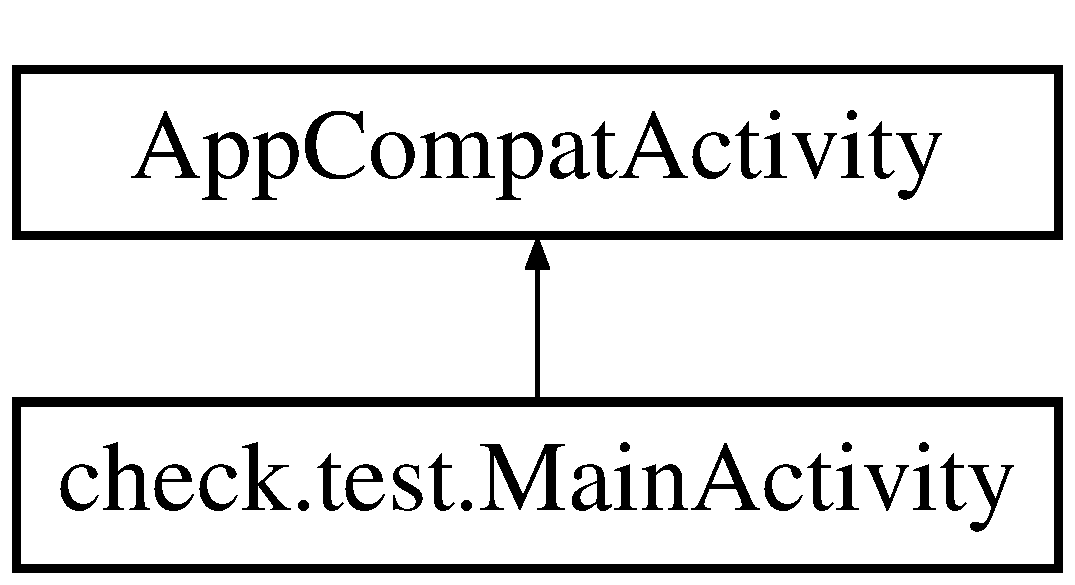
\includegraphics[height=2.000000cm]{classcheck_1_1test_1_1_main_activity}
\end{center}
\end{figure}
\subsection*{Public Member Functions}
\begin{DoxyCompactItemize}
\item 
\hypertarget{classcheck_1_1test_1_1_main_activity_aaafdc43b53167e93a6820e2e61f52c9c}{}boolean {\bfseries on\+Options\+Item\+Selected} (Menu\+Item item)\label{classcheck_1_1test_1_1_main_activity_aaafdc43b53167e93a6820e2e61f52c9c}

\item 
boolean \hyperlink{classcheck_1_1test_1_1_main_activity_a32779498a0628d0b7a6a95f503210c1a}{on\+Create\+Options\+Menu} (Menu menu)
\end{DoxyCompactItemize}
\subsection*{Protected Member Functions}
\begin{DoxyCompactItemize}
\item 
\hypertarget{classcheck_1_1test_1_1_main_activity_a57b96b92e4a448b3cb26c318310c7d23}{}void {\bfseries on\+Create} (Bundle saved\+Instance\+State)\label{classcheck_1_1test_1_1_main_activity_a57b96b92e4a448b3cb26c318310c7d23}

\end{DoxyCompactItemize}


\subsection{Detailed Description}
First Application Page. 

Created when Application first starts. Lays out profile settings if user settings are set to null.

Presss anywhere on screen leads to the second screen, the \hyperlink{classcheck_1_1test_1_1_creation_screen}{Creation\+Screen} activity. 

\subsection{Member Function Documentation}
\hypertarget{classcheck_1_1test_1_1_main_activity_a32779498a0628d0b7a6a95f503210c1a}{}\index{check\+::test\+::\+Main\+Activity@{check\+::test\+::\+Main\+Activity}!on\+Create\+Options\+Menu@{on\+Create\+Options\+Menu}}
\index{on\+Create\+Options\+Menu@{on\+Create\+Options\+Menu}!check\+::test\+::\+Main\+Activity@{check\+::test\+::\+Main\+Activity}}
\subsubsection[{on\+Create\+Options\+Menu(\+Menu menu)}]{\setlength{\rightskip}{0pt plus 5cm}boolean check.\+test.\+Main\+Activity.\+on\+Create\+Options\+Menu (
\begin{DoxyParamCaption}
\item[{Menu}]{menu}
\end{DoxyParamCaption}
)}\label{classcheck_1_1test_1_1_main_activity_a32779498a0628d0b7a6a95f503210c1a}
dfdsfdsafdsafdsafdsaf

Detailed description of file. 

The documentation for this class was generated from the following file\+:\begin{DoxyCompactItemize}
\item 
C\+:/\+Users/\+Zwretched/.\+Android\+Studio1.\+4/\+Projects/\+Dress\+Me\+\_\+\+Android/\+Dress\+Me/src/main/java/check/test/Main\+Activity.\+java\end{DoxyCompactItemize}

\hypertarget{classcheck_1_1test_1_1_r_1_1menu}{}\section{check.\+test.\+R.\+menu Class Reference}
\label{classcheck_1_1test_1_1_r_1_1menu}\index{check.\+test.\+R.\+menu@{check.\+test.\+R.\+menu}}
\subsection*{Static Public Attributes}
\begin{DoxyCompactItemize}
\item 
\hypertarget{classcheck_1_1test_1_1_r_1_1menu_ade2d72708302b3b85aa2f9f1b952262f}{}static final int {\bfseries menu\+\_\+main} =0x7f0d0000\label{classcheck_1_1test_1_1_r_1_1menu_ade2d72708302b3b85aa2f9f1b952262f}

\end{DoxyCompactItemize}


The documentation for this class was generated from the following file\+:\begin{DoxyCompactItemize}
\item 
C\+:/\+Users/\+Zwretched/.\+Android\+Studio1.\+4/\+Projects/\+Dress\+Me\+\_\+\+Android/\+Dress\+Me/build/generated/source/r/debug/check/test/R.\+java\end{DoxyCompactItemize}

\hypertarget{classcheck_1_1test_1_1_r_1_1mipmap}{}\section{check.\+test.\+R.\+mipmap Class Reference}
\label{classcheck_1_1test_1_1_r_1_1mipmap}\index{check.\+test.\+R.\+mipmap@{check.\+test.\+R.\+mipmap}}
\subsection*{Static Public Attributes}
\begin{DoxyCompactItemize}
\item 
\hypertarget{classcheck_1_1test_1_1_r_1_1mipmap_ae5cc040210eaf00cf2d3c5cb0950bbc1}{}static final int {\bfseries ic\+\_\+launcher} =0x7f030000\label{classcheck_1_1test_1_1_r_1_1mipmap_ae5cc040210eaf00cf2d3c5cb0950bbc1}

\end{DoxyCompactItemize}


The documentation for this class was generated from the following file\+:\begin{DoxyCompactItemize}
\item 
C\+:/\+Users/\+Zwretched/.\+Android\+Studio1.\+4/\+Projects/\+Dress\+Me\+\_\+\+Android/\+Dress\+Me/build/generated/source/r/debug/check/test/R.\+java\end{DoxyCompactItemize}

\hypertarget{classandroid_1_1support_1_1v7_1_1appcompat_1_1_r}{}\section{android.\+support.\+v7.\+appcompat.\+R Class Reference}
\label{classandroid_1_1support_1_1v7_1_1appcompat_1_1_r}\index{android.\+support.\+v7.\+appcompat.\+R@{android.\+support.\+v7.\+appcompat.\+R}}
\subsection*{Classes}
\begin{DoxyCompactItemize}
\item 
class \hyperlink{classandroid_1_1support_1_1v7_1_1appcompat_1_1_r_1_1anim}{anim}
\item 
class \hyperlink{classandroid_1_1support_1_1v7_1_1appcompat_1_1_r_1_1attr}{attr}
\item 
class \hyperlink{classandroid_1_1support_1_1v7_1_1appcompat_1_1_r_1_1bool}{bool}
\item 
class \hyperlink{classandroid_1_1support_1_1v7_1_1appcompat_1_1_r_1_1color}{color}
\item 
class \hyperlink{classandroid_1_1support_1_1v7_1_1appcompat_1_1_r_1_1dimen}{dimen}
\item 
class \hyperlink{classandroid_1_1support_1_1v7_1_1appcompat_1_1_r_1_1drawable}{drawable}
\item 
class \hyperlink{classandroid_1_1support_1_1v7_1_1appcompat_1_1_r_1_1id}{id}
\item 
class \hyperlink{classandroid_1_1support_1_1v7_1_1appcompat_1_1_r_1_1integer}{integer}
\item 
class \hyperlink{classandroid_1_1support_1_1v7_1_1appcompat_1_1_r_1_1layout}{layout}
\item 
class \hyperlink{classandroid_1_1support_1_1v7_1_1appcompat_1_1_r_1_1string}{string}
\item 
class \hyperlink{classandroid_1_1support_1_1v7_1_1appcompat_1_1_r_1_1style}{style}
\item 
class \hyperlink{classandroid_1_1support_1_1v7_1_1appcompat_1_1_r_1_1styleable}{styleable}
\end{DoxyCompactItemize}


The documentation for this class was generated from the following file\+:\begin{DoxyCompactItemize}
\item 
C\+:/\+Users/\+Zwretched/.\+Android\+Studio1.\+4/\+Projects/\+Dress\+Me\+\_\+\+Android/\+Dress\+Me/build/generated/source/r/debug/android/support/v7/appcompat/R.\+java\end{DoxyCompactItemize}

\hypertarget{classcheck_1_1test_1_1_r}{}\section{check.\+test.\+R Class Reference}
\label{classcheck_1_1test_1_1_r}\index{check.\+test.\+R@{check.\+test.\+R}}
\subsection*{Classes}
\begin{DoxyCompactItemize}
\item 
class \hyperlink{classcheck_1_1test_1_1_r_1_1anim}{anim}
\item 
class \hyperlink{classcheck_1_1test_1_1_r_1_1attr}{attr}
\item 
class \hyperlink{classcheck_1_1test_1_1_r_1_1bool}{bool}
\item 
class \hyperlink{classcheck_1_1test_1_1_r_1_1color}{color}
\item 
class \hyperlink{classcheck_1_1test_1_1_r_1_1dimen}{dimen}
\item 
class \hyperlink{classcheck_1_1test_1_1_r_1_1drawable}{drawable}
\item 
class \hyperlink{classcheck_1_1test_1_1_r_1_1id}{id}
\item 
class \hyperlink{classcheck_1_1test_1_1_r_1_1integer}{integer}
\item 
class \hyperlink{classcheck_1_1test_1_1_r_1_1layout}{layout}
\item 
class \hyperlink{classcheck_1_1test_1_1_r_1_1menu}{menu}
\item 
class \hyperlink{classcheck_1_1test_1_1_r_1_1mipmap}{mipmap}
\item 
class \hyperlink{classcheck_1_1test_1_1_r_1_1string}{string}
\item 
class \hyperlink{classcheck_1_1test_1_1_r_1_1style}{style}
\item 
class \hyperlink{classcheck_1_1test_1_1_r_1_1styleable}{styleable}
\end{DoxyCompactItemize}


The documentation for this class was generated from the following file\+:\begin{DoxyCompactItemize}
\item 
C\+:/\+Users/\+Zwretched/.\+Android\+Studio1.\+4/\+Projects/\+Dress\+Me\+\_\+\+Android/\+Dress\+Me/build/generated/source/r/debug/check/test/R.\+java\end{DoxyCompactItemize}

\hypertarget{classandroid_1_1support_1_1design_1_1_r}{}\section{android.\+support.\+design.\+R Class Reference}
\label{classandroid_1_1support_1_1design_1_1_r}\index{android.\+support.\+design.\+R@{android.\+support.\+design.\+R}}
\subsection*{Classes}
\begin{DoxyCompactItemize}
\item 
class \hyperlink{classandroid_1_1support_1_1design_1_1_r_1_1anim}{anim}
\item 
class \hyperlink{classandroid_1_1support_1_1design_1_1_r_1_1attr}{attr}
\item 
class \hyperlink{classandroid_1_1support_1_1design_1_1_r_1_1bool}{bool}
\item 
class \hyperlink{classandroid_1_1support_1_1design_1_1_r_1_1color}{color}
\item 
class \hyperlink{classandroid_1_1support_1_1design_1_1_r_1_1dimen}{dimen}
\item 
class \hyperlink{classandroid_1_1support_1_1design_1_1_r_1_1drawable}{drawable}
\item 
class \hyperlink{classandroid_1_1support_1_1design_1_1_r_1_1id}{id}
\item 
class \hyperlink{classandroid_1_1support_1_1design_1_1_r_1_1integer}{integer}
\item 
class \hyperlink{classandroid_1_1support_1_1design_1_1_r_1_1layout}{layout}
\item 
class \hyperlink{classandroid_1_1support_1_1design_1_1_r_1_1string}{string}
\item 
class \hyperlink{classandroid_1_1support_1_1design_1_1_r_1_1style}{style}
\item 
class \hyperlink{classandroid_1_1support_1_1design_1_1_r_1_1styleable}{styleable}
\end{DoxyCompactItemize}


The documentation for this class was generated from the following file\+:\begin{DoxyCompactItemize}
\item 
C\+:/\+Users/\+Zwretched/.\+Android\+Studio1.\+4/\+Projects/\+Dress\+Me\+\_\+\+Android/\+Dress\+Me/build/generated/source/r/debug/android/support/design/R.\+java\end{DoxyCompactItemize}

\hypertarget{classandroid_1_1support_1_1design_1_1_r_1_1string}{}\section{android.\+support.\+design.\+R.\+string Class Reference}
\label{classandroid_1_1support_1_1design_1_1_r_1_1string}\index{android.\+support.\+design.\+R.\+string@{android.\+support.\+design.\+R.\+string}}
\subsection*{Static Public Attributes}
\begin{DoxyCompactItemize}
\item 
\hypertarget{classandroid_1_1support_1_1design_1_1_r_1_1string_ae94186933fbea8b608ced5c610548d2e}{}static final int {\bfseries abc\+\_\+action\+\_\+bar\+\_\+home\+\_\+description} = 0x7f060000\label{classandroid_1_1support_1_1design_1_1_r_1_1string_ae94186933fbea8b608ced5c610548d2e}

\item 
\hypertarget{classandroid_1_1support_1_1design_1_1_r_1_1string_aec1855ecfa354e84067b7fca0aa1a8de}{}static final int {\bfseries abc\+\_\+action\+\_\+bar\+\_\+home\+\_\+description\+\_\+format} = 0x7f060001\label{classandroid_1_1support_1_1design_1_1_r_1_1string_aec1855ecfa354e84067b7fca0aa1a8de}

\item 
\hypertarget{classandroid_1_1support_1_1design_1_1_r_1_1string_abf2c1e6008ec0466820d6998146bd96c}{}static final int {\bfseries abc\+\_\+action\+\_\+bar\+\_\+home\+\_\+subtitle\+\_\+description\+\_\+format} = 0x7f060002\label{classandroid_1_1support_1_1design_1_1_r_1_1string_abf2c1e6008ec0466820d6998146bd96c}

\item 
\hypertarget{classandroid_1_1support_1_1design_1_1_r_1_1string_a6879bf96dd0f053bc7b186fe5cc8fc3a}{}static final int {\bfseries abc\+\_\+action\+\_\+bar\+\_\+up\+\_\+description} = 0x7f060003\label{classandroid_1_1support_1_1design_1_1_r_1_1string_a6879bf96dd0f053bc7b186fe5cc8fc3a}

\item 
\hypertarget{classandroid_1_1support_1_1design_1_1_r_1_1string_a0da53f31459d40d1c77cb1a7e89746cb}{}static final int {\bfseries abc\+\_\+action\+\_\+menu\+\_\+overflow\+\_\+description} = 0x7f060004\label{classandroid_1_1support_1_1design_1_1_r_1_1string_a0da53f31459d40d1c77cb1a7e89746cb}

\item 
\hypertarget{classandroid_1_1support_1_1design_1_1_r_1_1string_a650cb796af0ed2ed3305583ac1887224}{}static final int {\bfseries abc\+\_\+action\+\_\+mode\+\_\+done} = 0x7f060005\label{classandroid_1_1support_1_1design_1_1_r_1_1string_a650cb796af0ed2ed3305583ac1887224}

\item 
\hypertarget{classandroid_1_1support_1_1design_1_1_r_1_1string_a9b4629898f289df4ea77edefdf9f011f}{}static final int {\bfseries abc\+\_\+activity\+\_\+chooser\+\_\+view\+\_\+see\+\_\+all} = 0x7f060006\label{classandroid_1_1support_1_1design_1_1_r_1_1string_a9b4629898f289df4ea77edefdf9f011f}

\item 
\hypertarget{classandroid_1_1support_1_1design_1_1_r_1_1string_a79f096c86588827bd6ad855469b5e54b}{}static final int {\bfseries abc\+\_\+activitychooserview\+\_\+choose\+\_\+application} = 0x7f060007\label{classandroid_1_1support_1_1design_1_1_r_1_1string_a79f096c86588827bd6ad855469b5e54b}

\item 
\hypertarget{classandroid_1_1support_1_1design_1_1_r_1_1string_a49cacb037d06f1b5b99ad9093a9a78e5}{}static final int {\bfseries abc\+\_\+search\+\_\+hint} = 0x7f060008\label{classandroid_1_1support_1_1design_1_1_r_1_1string_a49cacb037d06f1b5b99ad9093a9a78e5}

\item 
\hypertarget{classandroid_1_1support_1_1design_1_1_r_1_1string_ada43ec0fa6465dcc33878e45bd9d0fdf}{}static final int {\bfseries abc\+\_\+searchview\+\_\+description\+\_\+clear} = 0x7f060009\label{classandroid_1_1support_1_1design_1_1_r_1_1string_ada43ec0fa6465dcc33878e45bd9d0fdf}

\item 
\hypertarget{classandroid_1_1support_1_1design_1_1_r_1_1string_a02e8b7161ffa91e25f2f8623cec6b2cf}{}static final int {\bfseries abc\+\_\+searchview\+\_\+description\+\_\+query} = 0x7f06000a\label{classandroid_1_1support_1_1design_1_1_r_1_1string_a02e8b7161ffa91e25f2f8623cec6b2cf}

\item 
\hypertarget{classandroid_1_1support_1_1design_1_1_r_1_1string_a6bf26a757b0d4c764952cc3795158341}{}static final int {\bfseries abc\+\_\+searchview\+\_\+description\+\_\+search} = 0x7f06000b\label{classandroid_1_1support_1_1design_1_1_r_1_1string_a6bf26a757b0d4c764952cc3795158341}

\item 
\hypertarget{classandroid_1_1support_1_1design_1_1_r_1_1string_a86402c10a07ce0ef57379f1e52663aeb}{}static final int {\bfseries abc\+\_\+searchview\+\_\+description\+\_\+submit} = 0x7f06000c\label{classandroid_1_1support_1_1design_1_1_r_1_1string_a86402c10a07ce0ef57379f1e52663aeb}

\item 
\hypertarget{classandroid_1_1support_1_1design_1_1_r_1_1string_a04a007dba1181292400d15625e31353a}{}static final int {\bfseries abc\+\_\+searchview\+\_\+description\+\_\+voice} = 0x7f06000d\label{classandroid_1_1support_1_1design_1_1_r_1_1string_a04a007dba1181292400d15625e31353a}

\item 
\hypertarget{classandroid_1_1support_1_1design_1_1_r_1_1string_a77ff2da70667bbe5ae57ebdbdc2738ea}{}static final int {\bfseries abc\+\_\+shareactionprovider\+\_\+share\+\_\+with} = 0x7f06000e\label{classandroid_1_1support_1_1design_1_1_r_1_1string_a77ff2da70667bbe5ae57ebdbdc2738ea}

\item 
\hypertarget{classandroid_1_1support_1_1design_1_1_r_1_1string_abe49db143c1d58a411f52de9775ac1f8}{}static final int {\bfseries abc\+\_\+shareactionprovider\+\_\+share\+\_\+with\+\_\+application} = 0x7f06000f\label{classandroid_1_1support_1_1design_1_1_r_1_1string_abe49db143c1d58a411f52de9775ac1f8}

\item 
\hypertarget{classandroid_1_1support_1_1design_1_1_r_1_1string_a1eb7e00e0658289be2b77468cd353b75}{}static final int {\bfseries abc\+\_\+toolbar\+\_\+collapse\+\_\+description} = 0x7f060010\label{classandroid_1_1support_1_1design_1_1_r_1_1string_a1eb7e00e0658289be2b77468cd353b75}

\item 
\hypertarget{classandroid_1_1support_1_1design_1_1_r_1_1string_a87a9e93b543f76960b86c5e59fd5a9d0}{}static final int {\bfseries appbar\+\_\+scrolling\+\_\+view\+\_\+behavior} = 0x7f060015\label{classandroid_1_1support_1_1design_1_1_r_1_1string_a87a9e93b543f76960b86c5e59fd5a9d0}

\item 
\hypertarget{classandroid_1_1support_1_1design_1_1_r_1_1string_ae7e600aba7d20d01b5e3b4ccc3847bc9}{}static final int {\bfseries status\+\_\+bar\+\_\+notification\+\_\+info\+\_\+overflow} = 0x7f060011\label{classandroid_1_1support_1_1design_1_1_r_1_1string_ae7e600aba7d20d01b5e3b4ccc3847bc9}

\end{DoxyCompactItemize}


The documentation for this class was generated from the following file\+:\begin{DoxyCompactItemize}
\item 
C\+:/\+Users/\+Zwretched/.\+Android\+Studio1.\+4/\+Projects/\+Dress\+Me\+\_\+\+Android/\+Dress\+Me/build/generated/source/r/debug/android/support/design/R.\+java\end{DoxyCompactItemize}

\hypertarget{classandroid_1_1support_1_1v7_1_1appcompat_1_1_r_1_1string}{}\section{android.\+support.\+v7.\+appcompat.\+R.\+string Class Reference}
\label{classandroid_1_1support_1_1v7_1_1appcompat_1_1_r_1_1string}\index{android.\+support.\+v7.\+appcompat.\+R.\+string@{android.\+support.\+v7.\+appcompat.\+R.\+string}}
\subsection*{Static Public Attributes}
\begin{DoxyCompactItemize}
\item 
\hypertarget{classandroid_1_1support_1_1v7_1_1appcompat_1_1_r_1_1string_ab2d2b1d0da0214cbe08414e3b8aeead9}{}static final int {\bfseries abc\+\_\+action\+\_\+bar\+\_\+home\+\_\+description} = 0x7f060000\label{classandroid_1_1support_1_1v7_1_1appcompat_1_1_r_1_1string_ab2d2b1d0da0214cbe08414e3b8aeead9}

\item 
\hypertarget{classandroid_1_1support_1_1v7_1_1appcompat_1_1_r_1_1string_ad59fccdbb8ada7347f02ffdb92d7da9c}{}static final int {\bfseries abc\+\_\+action\+\_\+bar\+\_\+home\+\_\+description\+\_\+format} = 0x7f060001\label{classandroid_1_1support_1_1v7_1_1appcompat_1_1_r_1_1string_ad59fccdbb8ada7347f02ffdb92d7da9c}

\item 
\hypertarget{classandroid_1_1support_1_1v7_1_1appcompat_1_1_r_1_1string_ab301aa506d8cfcf2cb74a816212deb90}{}static final int {\bfseries abc\+\_\+action\+\_\+bar\+\_\+home\+\_\+subtitle\+\_\+description\+\_\+format} = 0x7f060002\label{classandroid_1_1support_1_1v7_1_1appcompat_1_1_r_1_1string_ab301aa506d8cfcf2cb74a816212deb90}

\item 
\hypertarget{classandroid_1_1support_1_1v7_1_1appcompat_1_1_r_1_1string_a3a4f65bf9f2bdae055c146bca7613520}{}static final int {\bfseries abc\+\_\+action\+\_\+bar\+\_\+up\+\_\+description} = 0x7f060003\label{classandroid_1_1support_1_1v7_1_1appcompat_1_1_r_1_1string_a3a4f65bf9f2bdae055c146bca7613520}

\item 
\hypertarget{classandroid_1_1support_1_1v7_1_1appcompat_1_1_r_1_1string_a3985456499fd328f556a626481695499}{}static final int {\bfseries abc\+\_\+action\+\_\+menu\+\_\+overflow\+\_\+description} = 0x7f060004\label{classandroid_1_1support_1_1v7_1_1appcompat_1_1_r_1_1string_a3985456499fd328f556a626481695499}

\item 
\hypertarget{classandroid_1_1support_1_1v7_1_1appcompat_1_1_r_1_1string_ab47aea7d6f590078f9b103b739084828}{}static final int {\bfseries abc\+\_\+action\+\_\+mode\+\_\+done} = 0x7f060005\label{classandroid_1_1support_1_1v7_1_1appcompat_1_1_r_1_1string_ab47aea7d6f590078f9b103b739084828}

\item 
\hypertarget{classandroid_1_1support_1_1v7_1_1appcompat_1_1_r_1_1string_a251b3261b9f1bd9fe85117e02d81d6a8}{}static final int {\bfseries abc\+\_\+activity\+\_\+chooser\+\_\+view\+\_\+see\+\_\+all} = 0x7f060006\label{classandroid_1_1support_1_1v7_1_1appcompat_1_1_r_1_1string_a251b3261b9f1bd9fe85117e02d81d6a8}

\item 
\hypertarget{classandroid_1_1support_1_1v7_1_1appcompat_1_1_r_1_1string_a90f4fe7b227c4fbf744928e926fbea60}{}static final int {\bfseries abc\+\_\+activitychooserview\+\_\+choose\+\_\+application} = 0x7f060007\label{classandroid_1_1support_1_1v7_1_1appcompat_1_1_r_1_1string_a90f4fe7b227c4fbf744928e926fbea60}

\item 
\hypertarget{classandroid_1_1support_1_1v7_1_1appcompat_1_1_r_1_1string_a8a977c43ae9b6036b792a424d60ff3ed}{}static final int {\bfseries abc\+\_\+search\+\_\+hint} = 0x7f060008\label{classandroid_1_1support_1_1v7_1_1appcompat_1_1_r_1_1string_a8a977c43ae9b6036b792a424d60ff3ed}

\item 
\hypertarget{classandroid_1_1support_1_1v7_1_1appcompat_1_1_r_1_1string_a458a8ba55dea450ed52e936d7fbb4312}{}static final int {\bfseries abc\+\_\+searchview\+\_\+description\+\_\+clear} = 0x7f060009\label{classandroid_1_1support_1_1v7_1_1appcompat_1_1_r_1_1string_a458a8ba55dea450ed52e936d7fbb4312}

\item 
\hypertarget{classandroid_1_1support_1_1v7_1_1appcompat_1_1_r_1_1string_a687a6a0f890080c34188b0570f1ad557}{}static final int {\bfseries abc\+\_\+searchview\+\_\+description\+\_\+query} = 0x7f06000a\label{classandroid_1_1support_1_1v7_1_1appcompat_1_1_r_1_1string_a687a6a0f890080c34188b0570f1ad557}

\item 
\hypertarget{classandroid_1_1support_1_1v7_1_1appcompat_1_1_r_1_1string_adb0d54ee3eeb2609de19decfc0831c19}{}static final int {\bfseries abc\+\_\+searchview\+\_\+description\+\_\+search} = 0x7f06000b\label{classandroid_1_1support_1_1v7_1_1appcompat_1_1_r_1_1string_adb0d54ee3eeb2609de19decfc0831c19}

\item 
\hypertarget{classandroid_1_1support_1_1v7_1_1appcompat_1_1_r_1_1string_ae42251191872922dcd3e42a02b86f36c}{}static final int {\bfseries abc\+\_\+searchview\+\_\+description\+\_\+submit} = 0x7f06000c\label{classandroid_1_1support_1_1v7_1_1appcompat_1_1_r_1_1string_ae42251191872922dcd3e42a02b86f36c}

\item 
\hypertarget{classandroid_1_1support_1_1v7_1_1appcompat_1_1_r_1_1string_af44447786247cf4c993ba7d749a18d7b}{}static final int {\bfseries abc\+\_\+searchview\+\_\+description\+\_\+voice} = 0x7f06000d\label{classandroid_1_1support_1_1v7_1_1appcompat_1_1_r_1_1string_af44447786247cf4c993ba7d749a18d7b}

\item 
\hypertarget{classandroid_1_1support_1_1v7_1_1appcompat_1_1_r_1_1string_ada3024d7f8a977c5a49a8cab63c26f27}{}static final int {\bfseries abc\+\_\+shareactionprovider\+\_\+share\+\_\+with} = 0x7f06000e\label{classandroid_1_1support_1_1v7_1_1appcompat_1_1_r_1_1string_ada3024d7f8a977c5a49a8cab63c26f27}

\item 
\hypertarget{classandroid_1_1support_1_1v7_1_1appcompat_1_1_r_1_1string_acd327651d6f2bbab98396d2967431584}{}static final int {\bfseries abc\+\_\+shareactionprovider\+\_\+share\+\_\+with\+\_\+application} = 0x7f06000f\label{classandroid_1_1support_1_1v7_1_1appcompat_1_1_r_1_1string_acd327651d6f2bbab98396d2967431584}

\item 
\hypertarget{classandroid_1_1support_1_1v7_1_1appcompat_1_1_r_1_1string_a399ac8dfa9600f2c34e5d9f2d3e78edb}{}static final int {\bfseries abc\+\_\+toolbar\+\_\+collapse\+\_\+description} = 0x7f060010\label{classandroid_1_1support_1_1v7_1_1appcompat_1_1_r_1_1string_a399ac8dfa9600f2c34e5d9f2d3e78edb}

\item 
\hypertarget{classandroid_1_1support_1_1v7_1_1appcompat_1_1_r_1_1string_a7cc8e172b664c63f22e7d64dab601204}{}static final int {\bfseries status\+\_\+bar\+\_\+notification\+\_\+info\+\_\+overflow} = 0x7f060011\label{classandroid_1_1support_1_1v7_1_1appcompat_1_1_r_1_1string_a7cc8e172b664c63f22e7d64dab601204}

\end{DoxyCompactItemize}


The documentation for this class was generated from the following file\+:\begin{DoxyCompactItemize}
\item 
C\+:/\+Users/\+Zwretched/.\+Android\+Studio1.\+4/\+Projects/\+Dress\+Me\+\_\+\+Android/\+Dress\+Me/build/generated/source/r/debug/android/support/v7/appcompat/R.\+java\end{DoxyCompactItemize}

\hypertarget{classcheck_1_1test_1_1_r_1_1string}{}\section{check.\+test.\+R.\+string Class Reference}
\label{classcheck_1_1test_1_1_r_1_1string}\index{check.\+test.\+R.\+string@{check.\+test.\+R.\+string}}
\subsection*{Static Public Attributes}
\begin{DoxyCompactItemize}
\item 
\hypertarget{classcheck_1_1test_1_1_r_1_1string_a86e5d90ea8e8a49edb01af69da14c227}{}static final int {\bfseries abc\+\_\+action\+\_\+bar\+\_\+home\+\_\+description} =0x7f060000\label{classcheck_1_1test_1_1_r_1_1string_a86e5d90ea8e8a49edb01af69da14c227}

\item 
\hypertarget{classcheck_1_1test_1_1_r_1_1string_ab1f3342cbdaf9c8523440026d20f3264}{}static final int {\bfseries abc\+\_\+action\+\_\+bar\+\_\+home\+\_\+description\+\_\+format} =0x7f060001\label{classcheck_1_1test_1_1_r_1_1string_ab1f3342cbdaf9c8523440026d20f3264}

\item 
\hypertarget{classcheck_1_1test_1_1_r_1_1string_a7c31eb39813022b70740c17d1be810bb}{}static final int {\bfseries abc\+\_\+action\+\_\+bar\+\_\+home\+\_\+subtitle\+\_\+description\+\_\+format} =0x7f060002\label{classcheck_1_1test_1_1_r_1_1string_a7c31eb39813022b70740c17d1be810bb}

\item 
\hypertarget{classcheck_1_1test_1_1_r_1_1string_a06a09eb74b35a504e4b3ea6f401f85ec}{}static final int {\bfseries abc\+\_\+action\+\_\+bar\+\_\+up\+\_\+description} =0x7f060003\label{classcheck_1_1test_1_1_r_1_1string_a06a09eb74b35a504e4b3ea6f401f85ec}

\item 
\hypertarget{classcheck_1_1test_1_1_r_1_1string_aa65b86e148da12aada0eb00abde6b9d7}{}static final int {\bfseries abc\+\_\+action\+\_\+menu\+\_\+overflow\+\_\+description} =0x7f060004\label{classcheck_1_1test_1_1_r_1_1string_aa65b86e148da12aada0eb00abde6b9d7}

\item 
\hypertarget{classcheck_1_1test_1_1_r_1_1string_aad942d227094ee9555b1f092374ed08d}{}static final int {\bfseries abc\+\_\+action\+\_\+mode\+\_\+done} =0x7f060005\label{classcheck_1_1test_1_1_r_1_1string_aad942d227094ee9555b1f092374ed08d}

\item 
\hypertarget{classcheck_1_1test_1_1_r_1_1string_a392b85ef23b31e97c14bfa4b84031797}{}static final int {\bfseries abc\+\_\+activity\+\_\+chooser\+\_\+view\+\_\+see\+\_\+all} =0x7f060006\label{classcheck_1_1test_1_1_r_1_1string_a392b85ef23b31e97c14bfa4b84031797}

\item 
\hypertarget{classcheck_1_1test_1_1_r_1_1string_a6532280df6ff470928259256084000d9}{}static final int {\bfseries abc\+\_\+activitychooserview\+\_\+choose\+\_\+application} =0x7f060007\label{classcheck_1_1test_1_1_r_1_1string_a6532280df6ff470928259256084000d9}

\item 
\hypertarget{classcheck_1_1test_1_1_r_1_1string_a2783cfe5ced23bd37469283b8fedf489}{}static final int {\bfseries abc\+\_\+search\+\_\+hint} =0x7f060008\label{classcheck_1_1test_1_1_r_1_1string_a2783cfe5ced23bd37469283b8fedf489}

\item 
\hypertarget{classcheck_1_1test_1_1_r_1_1string_ad0fbe4b6ffe3eda07d59655e137b35f9}{}static final int {\bfseries abc\+\_\+searchview\+\_\+description\+\_\+clear} =0x7f060009\label{classcheck_1_1test_1_1_r_1_1string_ad0fbe4b6ffe3eda07d59655e137b35f9}

\item 
\hypertarget{classcheck_1_1test_1_1_r_1_1string_a2135dfe78026bcfac02ae3b3fd41be39}{}static final int {\bfseries abc\+\_\+searchview\+\_\+description\+\_\+query} =0x7f06000a\label{classcheck_1_1test_1_1_r_1_1string_a2135dfe78026bcfac02ae3b3fd41be39}

\item 
\hypertarget{classcheck_1_1test_1_1_r_1_1string_a2f566ffd4b7b28037385fedf038e2405}{}static final int {\bfseries abc\+\_\+searchview\+\_\+description\+\_\+search} =0x7f06000b\label{classcheck_1_1test_1_1_r_1_1string_a2f566ffd4b7b28037385fedf038e2405}

\item 
\hypertarget{classcheck_1_1test_1_1_r_1_1string_ae25f5749325ebf1afe15b1944063f767}{}static final int {\bfseries abc\+\_\+searchview\+\_\+description\+\_\+submit} =0x7f06000c\label{classcheck_1_1test_1_1_r_1_1string_ae25f5749325ebf1afe15b1944063f767}

\item 
\hypertarget{classcheck_1_1test_1_1_r_1_1string_afbba2d75e0ca63582059faafe2a3416c}{}static final int {\bfseries abc\+\_\+searchview\+\_\+description\+\_\+voice} =0x7f06000d\label{classcheck_1_1test_1_1_r_1_1string_afbba2d75e0ca63582059faafe2a3416c}

\item 
\hypertarget{classcheck_1_1test_1_1_r_1_1string_ad0e226d2671f310f311d7579a073e257}{}static final int {\bfseries abc\+\_\+shareactionprovider\+\_\+share\+\_\+with} =0x7f06000e\label{classcheck_1_1test_1_1_r_1_1string_ad0e226d2671f310f311d7579a073e257}

\item 
\hypertarget{classcheck_1_1test_1_1_r_1_1string_ad39b5416c42f054f1d913d6330e3131a}{}static final int {\bfseries abc\+\_\+shareactionprovider\+\_\+share\+\_\+with\+\_\+application} =0x7f06000f\label{classcheck_1_1test_1_1_r_1_1string_ad39b5416c42f054f1d913d6330e3131a}

\item 
\hypertarget{classcheck_1_1test_1_1_r_1_1string_a759f9f7b254e87a166ed6e0892594d7e}{}static final int {\bfseries abc\+\_\+toolbar\+\_\+collapse\+\_\+description} =0x7f060010\label{classcheck_1_1test_1_1_r_1_1string_a759f9f7b254e87a166ed6e0892594d7e}

\item 
\hypertarget{classcheck_1_1test_1_1_r_1_1string_a051cc9f3f54bce9fa8b5d17f6a3b20b6}{}static final int {\bfseries action\+\_\+settings} =0x7f060012\label{classcheck_1_1test_1_1_r_1_1string_a051cc9f3f54bce9fa8b5d17f6a3b20b6}

\item 
\hypertarget{classcheck_1_1test_1_1_r_1_1string_a8fcabd9976e3f0efa6f3589dcf949aa7}{}static final int {\bfseries activity2\+\_\+title} =0x7f060013\label{classcheck_1_1test_1_1_r_1_1string_a8fcabd9976e3f0efa6f3589dcf949aa7}

\item 
\hypertarget{classcheck_1_1test_1_1_r_1_1string_ae462705a290824a117c2bc0918e431a4}{}static final int {\bfseries app\+\_\+name} =0x7f060014\label{classcheck_1_1test_1_1_r_1_1string_ae462705a290824a117c2bc0918e431a4}

\item 
\hypertarget{classcheck_1_1test_1_1_r_1_1string_a7d0f5592dc79602be92c9c031e2ea10a}{}static final int {\bfseries appbar\+\_\+scrolling\+\_\+view\+\_\+behavior} =0x7f060015\label{classcheck_1_1test_1_1_r_1_1string_a7d0f5592dc79602be92c9c031e2ea10a}

\item 
\hypertarget{classcheck_1_1test_1_1_r_1_1string_a55c948adb2c62fc0a3a8cd49ac476b83}{}static final int {\bfseries button\+\_\+accessory} =0x7f060016\label{classcheck_1_1test_1_1_r_1_1string_a55c948adb2c62fc0a3a8cd49ac476b83}

\item 
\hypertarget{classcheck_1_1test_1_1_r_1_1string_ac40cf867547a1c722bc24b220c4a5d00}{}static final int {\bfseries button\+\_\+legging} =0x7f060017\label{classcheck_1_1test_1_1_r_1_1string_ac40cf867547a1c722bc24b220c4a5d00}

\item 
\hypertarget{classcheck_1_1test_1_1_r_1_1string_a8d1e700915e475ef1aeca6307f7c99ee}{}static final int {\bfseries button\+\_\+shoe} =0x7f060018\label{classcheck_1_1test_1_1_r_1_1string_a8d1e700915e475ef1aeca6307f7c99ee}

\item 
\hypertarget{classcheck_1_1test_1_1_r_1_1string_a81cda75b28654b9074a76be13bc92885}{}static final int {\bfseries button\+\_\+top} =0x7f060019\label{classcheck_1_1test_1_1_r_1_1string_a81cda75b28654b9074a76be13bc92885}

\item 
\hypertarget{classcheck_1_1test_1_1_r_1_1string_aa1f304bea36f9c9f911beae05102d1b9}{}static final int {\bfseries menu\+\_\+option1} =0x7f06001a\label{classcheck_1_1test_1_1_r_1_1string_aa1f304bea36f9c9f911beae05102d1b9}

\item 
\hypertarget{classcheck_1_1test_1_1_r_1_1string_ac28c5c90c2b2030ca07b353b79774242}{}static final int {\bfseries menu\+\_\+option2} =0x7f06001b\label{classcheck_1_1test_1_1_r_1_1string_ac28c5c90c2b2030ca07b353b79774242}

\item 
\hypertarget{classcheck_1_1test_1_1_r_1_1string_a6f49fc1afb69fa93b92d31ba04e1a292}{}static final int {\bfseries menu\+\_\+option3} =0x7f06001c\label{classcheck_1_1test_1_1_r_1_1string_a6f49fc1afb69fa93b92d31ba04e1a292}

\item 
\hypertarget{classcheck_1_1test_1_1_r_1_1string_a4650b8ee5f0db58e8bf3f1f460060ce0}{}static final int {\bfseries menu\+\_\+option4} =0x7f06001d\label{classcheck_1_1test_1_1_r_1_1string_a4650b8ee5f0db58e8bf3f1f460060ce0}

\item 
\hypertarget{classcheck_1_1test_1_1_r_1_1string_a72ff8159be4668cd0ba13d30ba353e8a}{}static final int {\bfseries menu\+\_\+option5} =0x7f06001e\label{classcheck_1_1test_1_1_r_1_1string_a72ff8159be4668cd0ba13d30ba353e8a}

\item 
\hypertarget{classcheck_1_1test_1_1_r_1_1string_a43b38ecc1f2f790948516b2ecb46803f}{}static final int {\bfseries menu\+\_\+option6} =0x7f06001f\label{classcheck_1_1test_1_1_r_1_1string_a43b38ecc1f2f790948516b2ecb46803f}

\item 
\hypertarget{classcheck_1_1test_1_1_r_1_1string_ad926501366f8da4c4bb8653a87c84783}{}static final int {\bfseries status\+\_\+bar\+\_\+notification\+\_\+info\+\_\+overflow} =0x7f060011\label{classcheck_1_1test_1_1_r_1_1string_ad926501366f8da4c4bb8653a87c84783}

\item 
\hypertarget{classcheck_1_1test_1_1_r_1_1string_a856306df2fb6c377343b4994f9c93e4a}{}static final int {\bfseries title\+\_\+activity\+\_\+creation\+\_\+screen} =0x7f060020\label{classcheck_1_1test_1_1_r_1_1string_a856306df2fb6c377343b4994f9c93e4a}

\item 
\hypertarget{classcheck_1_1test_1_1_r_1_1string_a21bd3d25d3f2c66a28a050c98edae11e}{}static final int {\bfseries title\+\_\+activity\+\_\+favorites} =0x7f060021\label{classcheck_1_1test_1_1_r_1_1string_a21bd3d25d3f2c66a28a050c98edae11e}

\item 
\hypertarget{classcheck_1_1test_1_1_r_1_1string_a654963115131d7a21c7f0610ff09ad2e}{}static final int {\bfseries title\+\_\+activity\+\_\+favorites2} =0x7f060022\label{classcheck_1_1test_1_1_r_1_1string_a654963115131d7a21c7f0610ff09ad2e}

\item 
\hypertarget{classcheck_1_1test_1_1_r_1_1string_af43fef5396cfcc85793c9c07479ef69f}{}static final int {\bfseries title\+\_\+activity\+\_\+gallery\+\_\+top} =0x7f060023\label{classcheck_1_1test_1_1_r_1_1string_af43fef5396cfcc85793c9c07479ef69f}

\item 
\hypertarget{classcheck_1_1test_1_1_r_1_1string_a430e0f72a973a0591e80dc8d3920fd07}{}static final int {\bfseries title\+\_\+activity\+\_\+gallerybutton\+\_\+\+\_\+top} =0x7f060024\label{classcheck_1_1test_1_1_r_1_1string_a430e0f72a973a0591e80dc8d3920fd07}

\item 
\hypertarget{classcheck_1_1test_1_1_r_1_1string_a7f8913f3256286e993ddde56ad2c4c48}{}static final int {\bfseries title\+\_\+activity\+\_\+main2} =0x7f060025\label{classcheck_1_1test_1_1_r_1_1string_a7f8913f3256286e993ddde56ad2c4c48}

\end{DoxyCompactItemize}


The documentation for this class was generated from the following file\+:\begin{DoxyCompactItemize}
\item 
C\+:/\+Users/\+Zwretched/.\+Android\+Studio1.\+4/\+Projects/\+Dress\+Me\+\_\+\+Android/\+Dress\+Me/build/generated/source/r/debug/check/test/R.\+java\end{DoxyCompactItemize}

\hypertarget{classcheck_1_1test_1_1_r_1_1style}{}\section{check.\+test.\+R.\+style Class Reference}
\label{classcheck_1_1test_1_1_r_1_1style}\index{check.\+test.\+R.\+style@{check.\+test.\+R.\+style}}
\subsection*{Static Public Attributes}
\begin{DoxyCompactItemize}
\item 
\hypertarget{classcheck_1_1test_1_1_r_1_1style_aa5d5dcbf14e27b682e2eebc4b98052b6}{}static final int {\bfseries Alert\+Dialog\+\_\+\+App\+Compat} =0x7f08007c\label{classcheck_1_1test_1_1_r_1_1style_aa5d5dcbf14e27b682e2eebc4b98052b6}

\item 
\hypertarget{classcheck_1_1test_1_1_r_1_1style_a042ebe50c854f5efb0a09e0e88baec30}{}static final int {\bfseries Alert\+Dialog\+\_\+\+App\+Compat\+\_\+\+Light} =0x7f08007d\label{classcheck_1_1test_1_1_r_1_1style_a042ebe50c854f5efb0a09e0e88baec30}

\item 
\hypertarget{classcheck_1_1test_1_1_r_1_1style_acdb3fe6bca8f5ba0e760a25d846ad093}{}static final int {\bfseries Animation\+\_\+\+App\+Compat\+\_\+\+Dialog} =0x7f08007e\label{classcheck_1_1test_1_1_r_1_1style_acdb3fe6bca8f5ba0e760a25d846ad093}

\item 
\hypertarget{classcheck_1_1test_1_1_r_1_1style_a529cd1dbbb2833b3b2058fec7c0a8f52}{}static final int {\bfseries Animation\+\_\+\+App\+Compat\+\_\+\+Drop\+Down\+Up} =0x7f08007f\label{classcheck_1_1test_1_1_r_1_1style_a529cd1dbbb2833b3b2058fec7c0a8f52}

\item 
\hypertarget{classcheck_1_1test_1_1_r_1_1style_ad089d681424fa4fcbf7bd30f978f7ff9}{}static final int {\bfseries App\+Theme} =0x7f080080\label{classcheck_1_1test_1_1_r_1_1style_ad089d681424fa4fcbf7bd30f978f7ff9}

\item 
\hypertarget{classcheck_1_1test_1_1_r_1_1style_a0047d0ca8442c354d0ba10572bd2c81b}{}static final int {\bfseries App\+Theme\+\_\+\+App\+Bar\+Overlay} =0x7f080081\label{classcheck_1_1test_1_1_r_1_1style_a0047d0ca8442c354d0ba10572bd2c81b}

\item 
\hypertarget{classcheck_1_1test_1_1_r_1_1style_a9292ba161b6075489472164a5cf195bb}{}static final int {\bfseries App\+Theme\+\_\+\+No\+Action\+Bar} =0x7f08002e\label{classcheck_1_1test_1_1_r_1_1style_a9292ba161b6075489472164a5cf195bb}

\item 
\hypertarget{classcheck_1_1test_1_1_r_1_1style_a06680ffe0a9ae57dd829f2c21eb24d7b}{}static final int {\bfseries App\+Theme\+\_\+\+Popup\+Overlay} =0x7f080082\label{classcheck_1_1test_1_1_r_1_1style_a06680ffe0a9ae57dd829f2c21eb24d7b}

\item 
\hypertarget{classcheck_1_1test_1_1_r_1_1style_aa81193c01e5080dcb553d01204a60daa}{}static final int {\bfseries Base\+\_\+\+Alert\+Dialog\+\_\+\+App\+Compat} =0x7f080083\label{classcheck_1_1test_1_1_r_1_1style_aa81193c01e5080dcb553d01204a60daa}

\item 
\hypertarget{classcheck_1_1test_1_1_r_1_1style_a71dd674f9c2679826553436190fceda8}{}static final int {\bfseries Base\+\_\+\+Alert\+Dialog\+\_\+\+App\+Compat\+\_\+\+Light} =0x7f080084\label{classcheck_1_1test_1_1_r_1_1style_a71dd674f9c2679826553436190fceda8}

\item 
\hypertarget{classcheck_1_1test_1_1_r_1_1style_ab20cea645087cb76e4f14e8d63b90265}{}static final int {\bfseries Base\+\_\+\+Animation\+\_\+\+App\+Compat\+\_\+\+Dialog} =0x7f080085\label{classcheck_1_1test_1_1_r_1_1style_ab20cea645087cb76e4f14e8d63b90265}

\item 
\hypertarget{classcheck_1_1test_1_1_r_1_1style_a534b652601a8e7c5ae3820bb44b87d5b}{}static final int {\bfseries Base\+\_\+\+Animation\+\_\+\+App\+Compat\+\_\+\+Drop\+Down\+Up} =0x7f080086\label{classcheck_1_1test_1_1_r_1_1style_a534b652601a8e7c5ae3820bb44b87d5b}

\item 
\hypertarget{classcheck_1_1test_1_1_r_1_1style_abcc1725cc5d2e50949915e3718120144}{}static final int {\bfseries Base\+\_\+\+Dialog\+Window\+Title\+\_\+\+App\+Compat} =0x7f080087\label{classcheck_1_1test_1_1_r_1_1style_abcc1725cc5d2e50949915e3718120144}

\item 
\hypertarget{classcheck_1_1test_1_1_r_1_1style_a35e0b1aed0b6b0f5352c1762be5b6868}{}static final int {\bfseries Base\+\_\+\+Dialog\+Window\+Title\+Background\+\_\+\+App\+Compat} =0x7f080088\label{classcheck_1_1test_1_1_r_1_1style_a35e0b1aed0b6b0f5352c1762be5b6868}

\item 
\hypertarget{classcheck_1_1test_1_1_r_1_1style_abeba811c0b41be4c85a30df7832ff3d3}{}static final int {\bfseries Base\+\_\+\+Text\+Appearance\+\_\+\+App\+Compat} =0x7f08002f\label{classcheck_1_1test_1_1_r_1_1style_abeba811c0b41be4c85a30df7832ff3d3}

\item 
\hypertarget{classcheck_1_1test_1_1_r_1_1style_a6c90194a77a5e8ecd671715fdeb8b10a}{}static final int {\bfseries Base\+\_\+\+Text\+Appearance\+\_\+\+App\+Compat\+\_\+\+Body1} =0x7f080030\label{classcheck_1_1test_1_1_r_1_1style_a6c90194a77a5e8ecd671715fdeb8b10a}

\item 
\hypertarget{classcheck_1_1test_1_1_r_1_1style_ac1858da6d242d2b38ed429fe849a2697}{}static final int {\bfseries Base\+\_\+\+Text\+Appearance\+\_\+\+App\+Compat\+\_\+\+Body2} =0x7f080031\label{classcheck_1_1test_1_1_r_1_1style_ac1858da6d242d2b38ed429fe849a2697}

\item 
\hypertarget{classcheck_1_1test_1_1_r_1_1style_ab95c66b3ff1555b885f72fef094e7a6d}{}static final int {\bfseries Base\+\_\+\+Text\+Appearance\+\_\+\+App\+Compat\+\_\+\+Button} =0x7f080019\label{classcheck_1_1test_1_1_r_1_1style_ab95c66b3ff1555b885f72fef094e7a6d}

\item 
\hypertarget{classcheck_1_1test_1_1_r_1_1style_ab400fc9a79c3061c993ebc0a8eafaabf}{}static final int {\bfseries Base\+\_\+\+Text\+Appearance\+\_\+\+App\+Compat\+\_\+\+Caption} =0x7f080032\label{classcheck_1_1test_1_1_r_1_1style_ab400fc9a79c3061c993ebc0a8eafaabf}

\item 
\hypertarget{classcheck_1_1test_1_1_r_1_1style_ad864d7092f1bdf3c1e22b388df1eb4f9}{}static final int {\bfseries Base\+\_\+\+Text\+Appearance\+\_\+\+App\+Compat\+\_\+\+Display1} =0x7f080033\label{classcheck_1_1test_1_1_r_1_1style_ad864d7092f1bdf3c1e22b388df1eb4f9}

\item 
\hypertarget{classcheck_1_1test_1_1_r_1_1style_a504a7f23ef9899334145689ea6495a52}{}static final int {\bfseries Base\+\_\+\+Text\+Appearance\+\_\+\+App\+Compat\+\_\+\+Display2} =0x7f080034\label{classcheck_1_1test_1_1_r_1_1style_a504a7f23ef9899334145689ea6495a52}

\item 
\hypertarget{classcheck_1_1test_1_1_r_1_1style_ab5a4f61262e06bf66e6d9e2cbdbc51ca}{}static final int {\bfseries Base\+\_\+\+Text\+Appearance\+\_\+\+App\+Compat\+\_\+\+Display3} =0x7f080035\label{classcheck_1_1test_1_1_r_1_1style_ab5a4f61262e06bf66e6d9e2cbdbc51ca}

\item 
\hypertarget{classcheck_1_1test_1_1_r_1_1style_aef765af3e5a55b1e1197bf77b34617f3}{}static final int {\bfseries Base\+\_\+\+Text\+Appearance\+\_\+\+App\+Compat\+\_\+\+Display4} =0x7f080036\label{classcheck_1_1test_1_1_r_1_1style_aef765af3e5a55b1e1197bf77b34617f3}

\item 
\hypertarget{classcheck_1_1test_1_1_r_1_1style_a1e2fd22e950a0446ded2a65fa4142d96}{}static final int {\bfseries Base\+\_\+\+Text\+Appearance\+\_\+\+App\+Compat\+\_\+\+Headline} =0x7f080037\label{classcheck_1_1test_1_1_r_1_1style_a1e2fd22e950a0446ded2a65fa4142d96}

\item 
\hypertarget{classcheck_1_1test_1_1_r_1_1style_acea5a87a415bce11a1890609b5406c6c}{}static final int {\bfseries Base\+\_\+\+Text\+Appearance\+\_\+\+App\+Compat\+\_\+\+Inverse} =0x7f080004\label{classcheck_1_1test_1_1_r_1_1style_acea5a87a415bce11a1890609b5406c6c}

\item 
\hypertarget{classcheck_1_1test_1_1_r_1_1style_af348a7c42fa565bf31c72cf897d70d2b}{}static final int {\bfseries Base\+\_\+\+Text\+Appearance\+\_\+\+App\+Compat\+\_\+\+Large} =0x7f080038\label{classcheck_1_1test_1_1_r_1_1style_af348a7c42fa565bf31c72cf897d70d2b}

\item 
\hypertarget{classcheck_1_1test_1_1_r_1_1style_a85b268aabca3f8addbcc82468081442e}{}static final int {\bfseries Base\+\_\+\+Text\+Appearance\+\_\+\+App\+Compat\+\_\+\+Large\+\_\+\+Inverse} =0x7f080005\label{classcheck_1_1test_1_1_r_1_1style_a85b268aabca3f8addbcc82468081442e}

\item 
\hypertarget{classcheck_1_1test_1_1_r_1_1style_ae00df87726b9bacfaafebf5a0763c0f9}{}static final int {\bfseries Base\+\_\+\+Text\+Appearance\+\_\+\+App\+Compat\+\_\+\+Light\+\_\+\+Widget\+\_\+\+Popup\+Menu\+\_\+\+Large} =0x7f080039\label{classcheck_1_1test_1_1_r_1_1style_ae00df87726b9bacfaafebf5a0763c0f9}

\item 
\hypertarget{classcheck_1_1test_1_1_r_1_1style_a415f8c2788b4bdb5011f007d4bc0b3cd}{}static final int {\bfseries Base\+\_\+\+Text\+Appearance\+\_\+\+App\+Compat\+\_\+\+Light\+\_\+\+Widget\+\_\+\+Popup\+Menu\+\_\+\+Small} =0x7f08003a\label{classcheck_1_1test_1_1_r_1_1style_a415f8c2788b4bdb5011f007d4bc0b3cd}

\item 
\hypertarget{classcheck_1_1test_1_1_r_1_1style_a17eae2fd8968c85f94575a10e3a4cae0}{}static final int {\bfseries Base\+\_\+\+Text\+Appearance\+\_\+\+App\+Compat\+\_\+\+Medium} =0x7f08003b\label{classcheck_1_1test_1_1_r_1_1style_a17eae2fd8968c85f94575a10e3a4cae0}

\item 
\hypertarget{classcheck_1_1test_1_1_r_1_1style_a91f69d25742572e4f29baec9a5304f7e}{}static final int {\bfseries Base\+\_\+\+Text\+Appearance\+\_\+\+App\+Compat\+\_\+\+Medium\+\_\+\+Inverse} =0x7f080006\label{classcheck_1_1test_1_1_r_1_1style_a91f69d25742572e4f29baec9a5304f7e}

\item 
\hypertarget{classcheck_1_1test_1_1_r_1_1style_a5abddc786b2ce11957b9c9f2794fd80b}{}static final int {\bfseries Base\+\_\+\+Text\+Appearance\+\_\+\+App\+Compat\+\_\+\+Menu} =0x7f08003c\label{classcheck_1_1test_1_1_r_1_1style_a5abddc786b2ce11957b9c9f2794fd80b}

\item 
\hypertarget{classcheck_1_1test_1_1_r_1_1style_a09b633323c8229b88d746767a1f2adf2}{}static final int {\bfseries Base\+\_\+\+Text\+Appearance\+\_\+\+App\+Compat\+\_\+\+Search\+Result} =0x7f080089\label{classcheck_1_1test_1_1_r_1_1style_a09b633323c8229b88d746767a1f2adf2}

\item 
\hypertarget{classcheck_1_1test_1_1_r_1_1style_a70147a8a83fd5f04808a91a5d2829a78}{}static final int {\bfseries Base\+\_\+\+Text\+Appearance\+\_\+\+App\+Compat\+\_\+\+Search\+Result\+\_\+\+Subtitle} =0x7f08003d\label{classcheck_1_1test_1_1_r_1_1style_a70147a8a83fd5f04808a91a5d2829a78}

\item 
\hypertarget{classcheck_1_1test_1_1_r_1_1style_a16772383ef71704cf1b8fb306c26a1f4}{}static final int {\bfseries Base\+\_\+\+Text\+Appearance\+\_\+\+App\+Compat\+\_\+\+Search\+Result\+\_\+\+Title} =0x7f08003e\label{classcheck_1_1test_1_1_r_1_1style_a16772383ef71704cf1b8fb306c26a1f4}

\item 
\hypertarget{classcheck_1_1test_1_1_r_1_1style_a54de5d881005e1a1fd60b061364aa0e3}{}static final int {\bfseries Base\+\_\+\+Text\+Appearance\+\_\+\+App\+Compat\+\_\+\+Small} =0x7f08003f\label{classcheck_1_1test_1_1_r_1_1style_a54de5d881005e1a1fd60b061364aa0e3}

\item 
\hypertarget{classcheck_1_1test_1_1_r_1_1style_a8daf8a76aadcd56a17eb952df1c7a05d}{}static final int {\bfseries Base\+\_\+\+Text\+Appearance\+\_\+\+App\+Compat\+\_\+\+Small\+\_\+\+Inverse} =0x7f080007\label{classcheck_1_1test_1_1_r_1_1style_a8daf8a76aadcd56a17eb952df1c7a05d}

\item 
\hypertarget{classcheck_1_1test_1_1_r_1_1style_a61b8708e0188da68c26accf58b5efd7f}{}static final int {\bfseries Base\+\_\+\+Text\+Appearance\+\_\+\+App\+Compat\+\_\+\+Subhead} =0x7f080040\label{classcheck_1_1test_1_1_r_1_1style_a61b8708e0188da68c26accf58b5efd7f}

\item 
\hypertarget{classcheck_1_1test_1_1_r_1_1style_ae1c1e1f374603df3adba4f2616f65334}{}static final int {\bfseries Base\+\_\+\+Text\+Appearance\+\_\+\+App\+Compat\+\_\+\+Subhead\+\_\+\+Inverse} =0x7f080008\label{classcheck_1_1test_1_1_r_1_1style_ae1c1e1f374603df3adba4f2616f65334}

\item 
\hypertarget{classcheck_1_1test_1_1_r_1_1style_a16794a9d3b49ef77a028478883b3083e}{}static final int {\bfseries Base\+\_\+\+Text\+Appearance\+\_\+\+App\+Compat\+\_\+\+Title} =0x7f080041\label{classcheck_1_1test_1_1_r_1_1style_a16794a9d3b49ef77a028478883b3083e}

\item 
\hypertarget{classcheck_1_1test_1_1_r_1_1style_a61d09d4e1ebff02bcbb8a157dff32942}{}static final int {\bfseries Base\+\_\+\+Text\+Appearance\+\_\+\+App\+Compat\+\_\+\+Title\+\_\+\+Inverse} =0x7f080009\label{classcheck_1_1test_1_1_r_1_1style_a61d09d4e1ebff02bcbb8a157dff32942}

\item 
\hypertarget{classcheck_1_1test_1_1_r_1_1style_a47ca56689b4a3c40894cff0e3ea334c9}{}static final int {\bfseries Base\+\_\+\+Text\+Appearance\+\_\+\+App\+Compat\+\_\+\+Widget\+\_\+\+Action\+Bar\+\_\+\+Menu} =0x7f080042\label{classcheck_1_1test_1_1_r_1_1style_a47ca56689b4a3c40894cff0e3ea334c9}

\item 
\hypertarget{classcheck_1_1test_1_1_r_1_1style_a951a6df09e499ec5394aa9602deac796}{}static final int {\bfseries Base\+\_\+\+Text\+Appearance\+\_\+\+App\+Compat\+\_\+\+Widget\+\_\+\+Action\+Bar\+\_\+\+Subtitle} =0x7f080043\label{classcheck_1_1test_1_1_r_1_1style_a951a6df09e499ec5394aa9602deac796}

\item 
\hypertarget{classcheck_1_1test_1_1_r_1_1style_a9027e6f82c577b17d83382d6e965f769}{}static final int {\bfseries Base\+\_\+\+Text\+Appearance\+\_\+\+App\+Compat\+\_\+\+Widget\+\_\+\+Action\+Bar\+\_\+\+Subtitle\+\_\+\+Inverse} =0x7f080044\label{classcheck_1_1test_1_1_r_1_1style_a9027e6f82c577b17d83382d6e965f769}

\item 
\hypertarget{classcheck_1_1test_1_1_r_1_1style_ac0bd71fb5b52c3de9a537c99677bc1cf}{}static final int {\bfseries Base\+\_\+\+Text\+Appearance\+\_\+\+App\+Compat\+\_\+\+Widget\+\_\+\+Action\+Bar\+\_\+\+Title} =0x7f080045\label{classcheck_1_1test_1_1_r_1_1style_ac0bd71fb5b52c3de9a537c99677bc1cf}

\item 
\hypertarget{classcheck_1_1test_1_1_r_1_1style_a7b7ca49b10f6acd4b23c2111c6968845}{}static final int {\bfseries Base\+\_\+\+Text\+Appearance\+\_\+\+App\+Compat\+\_\+\+Widget\+\_\+\+Action\+Bar\+\_\+\+Title\+\_\+\+Inverse} =0x7f080046\label{classcheck_1_1test_1_1_r_1_1style_a7b7ca49b10f6acd4b23c2111c6968845}

\item 
\hypertarget{classcheck_1_1test_1_1_r_1_1style_a927f77b0ee9a6f8278885711612cf765}{}static final int {\bfseries Base\+\_\+\+Text\+Appearance\+\_\+\+App\+Compat\+\_\+\+Widget\+\_\+\+Action\+Mode\+\_\+\+Subtitle} =0x7f080047\label{classcheck_1_1test_1_1_r_1_1style_a927f77b0ee9a6f8278885711612cf765}

\item 
\hypertarget{classcheck_1_1test_1_1_r_1_1style_a3d32f953db900f3314b45a0a3d7a911c}{}static final int {\bfseries Base\+\_\+\+Text\+Appearance\+\_\+\+App\+Compat\+\_\+\+Widget\+\_\+\+Action\+Mode\+\_\+\+Title} =0x7f080048\label{classcheck_1_1test_1_1_r_1_1style_a3d32f953db900f3314b45a0a3d7a911c}

\item 
\hypertarget{classcheck_1_1test_1_1_r_1_1style_a6cd0ce58949dc035ded88337dad6b404}{}static final int {\bfseries Base\+\_\+\+Text\+Appearance\+\_\+\+App\+Compat\+\_\+\+Widget\+\_\+\+Button} =0x7f080049\label{classcheck_1_1test_1_1_r_1_1style_a6cd0ce58949dc035ded88337dad6b404}

\item 
\hypertarget{classcheck_1_1test_1_1_r_1_1style_ad91bced4b6141b9c190089176f84fcdb}{}static final int {\bfseries Base\+\_\+\+Text\+Appearance\+\_\+\+App\+Compat\+\_\+\+Widget\+\_\+\+Button\+\_\+\+Inverse} =0x7f080078\label{classcheck_1_1test_1_1_r_1_1style_ad91bced4b6141b9c190089176f84fcdb}

\item 
\hypertarget{classcheck_1_1test_1_1_r_1_1style_a78274bb3f4d8d2f193357d3f1adbc7f2}{}static final int {\bfseries Base\+\_\+\+Text\+Appearance\+\_\+\+App\+Compat\+\_\+\+Widget\+\_\+\+Drop\+Down\+Item} =0x7f08008a\label{classcheck_1_1test_1_1_r_1_1style_a78274bb3f4d8d2f193357d3f1adbc7f2}

\item 
\hypertarget{classcheck_1_1test_1_1_r_1_1style_a106ef19fbba68ae2477c81250fabce4a}{}static final int {\bfseries Base\+\_\+\+Text\+Appearance\+\_\+\+App\+Compat\+\_\+\+Widget\+\_\+\+Popup\+Menu\+\_\+\+Large} =0x7f08004a\label{classcheck_1_1test_1_1_r_1_1style_a106ef19fbba68ae2477c81250fabce4a}

\item 
\hypertarget{classcheck_1_1test_1_1_r_1_1style_a6b6aa6530c111f85abf68b30a8536d53}{}static final int {\bfseries Base\+\_\+\+Text\+Appearance\+\_\+\+App\+Compat\+\_\+\+Widget\+\_\+\+Popup\+Menu\+\_\+\+Small} =0x7f08004b\label{classcheck_1_1test_1_1_r_1_1style_a6b6aa6530c111f85abf68b30a8536d53}

\item 
\hypertarget{classcheck_1_1test_1_1_r_1_1style_af825a9b419e94ec4a8fc1c1e444e344c}{}static final int {\bfseries Base\+\_\+\+Text\+Appearance\+\_\+\+App\+Compat\+\_\+\+Widget\+\_\+\+Switch} =0x7f08004c\label{classcheck_1_1test_1_1_r_1_1style_af825a9b419e94ec4a8fc1c1e444e344c}

\item 
\hypertarget{classcheck_1_1test_1_1_r_1_1style_aff7788fb3ebb26b04f5503458e66e9b8}{}static final int {\bfseries Base\+\_\+\+Text\+Appearance\+\_\+\+App\+Compat\+\_\+\+Widget\+\_\+\+Text\+View\+\_\+\+Spinner\+Item} =0x7f08004d\label{classcheck_1_1test_1_1_r_1_1style_aff7788fb3ebb26b04f5503458e66e9b8}

\item 
\hypertarget{classcheck_1_1test_1_1_r_1_1style_afcca64bbd946ab38e9dd1f3c155b0936}{}static final int {\bfseries Base\+\_\+\+Text\+Appearance\+\_\+\+Widget\+\_\+\+App\+Compat\+\_\+\+Expanded\+Menu\+\_\+\+Item} =0x7f08008b\label{classcheck_1_1test_1_1_r_1_1style_afcca64bbd946ab38e9dd1f3c155b0936}

\item 
\hypertarget{classcheck_1_1test_1_1_r_1_1style_a8e92eb2c88e987135a2ac2a595bb8eae}{}static final int {\bfseries Base\+\_\+\+Text\+Appearance\+\_\+\+Widget\+\_\+\+App\+Compat\+\_\+\+Toolbar\+\_\+\+Subtitle} =0x7f08004e\label{classcheck_1_1test_1_1_r_1_1style_a8e92eb2c88e987135a2ac2a595bb8eae}

\item 
\hypertarget{classcheck_1_1test_1_1_r_1_1style_ab09afe3962ba87a812f8b100645e98e0}{}static final int {\bfseries Base\+\_\+\+Text\+Appearance\+\_\+\+Widget\+\_\+\+App\+Compat\+\_\+\+Toolbar\+\_\+\+Title} =0x7f08004f\label{classcheck_1_1test_1_1_r_1_1style_ab09afe3962ba87a812f8b100645e98e0}

\item 
\hypertarget{classcheck_1_1test_1_1_r_1_1style_acf4e5cf32aba4bca0f1a9f609d166006}{}static final int {\bfseries Base\+\_\+\+Theme\+\_\+\+App\+Compat} =0x7f080050\label{classcheck_1_1test_1_1_r_1_1style_acf4e5cf32aba4bca0f1a9f609d166006}

\item 
\hypertarget{classcheck_1_1test_1_1_r_1_1style_a4e46a69a05be9af68dba55b7b0e65b47}{}static final int {\bfseries Base\+\_\+\+Theme\+\_\+\+App\+Compat\+\_\+\+Compact\+Menu} =0x7f08008c\label{classcheck_1_1test_1_1_r_1_1style_a4e46a69a05be9af68dba55b7b0e65b47}

\item 
\hypertarget{classcheck_1_1test_1_1_r_1_1style_ac1e61ded3bd391d39c6141c1fbd9243b}{}static final int {\bfseries Base\+\_\+\+Theme\+\_\+\+App\+Compat\+\_\+\+Dialog} =0x7f08000a\label{classcheck_1_1test_1_1_r_1_1style_ac1e61ded3bd391d39c6141c1fbd9243b}

\item 
\hypertarget{classcheck_1_1test_1_1_r_1_1style_a9522d2cdae5fbd28b7f4eb2fd029651f}{}static final int {\bfseries Base\+\_\+\+Theme\+\_\+\+App\+Compat\+\_\+\+Dialog\+\_\+\+Alert} =0x7f08008d\label{classcheck_1_1test_1_1_r_1_1style_a9522d2cdae5fbd28b7f4eb2fd029651f}

\item 
\hypertarget{classcheck_1_1test_1_1_r_1_1style_ae47d2b0638f74042b487347b9aba8e11}{}static final int {\bfseries Base\+\_\+\+Theme\+\_\+\+App\+Compat\+\_\+\+Dialog\+\_\+\+Fixed\+Size} =0x7f08008e\label{classcheck_1_1test_1_1_r_1_1style_ae47d2b0638f74042b487347b9aba8e11}

\item 
\hypertarget{classcheck_1_1test_1_1_r_1_1style_a4a754f5e0f533357864705d27c45ee77}{}static final int {\bfseries Base\+\_\+\+Theme\+\_\+\+App\+Compat\+\_\+\+Dialog\+\_\+\+Min\+Width} =0x7f08008f\label{classcheck_1_1test_1_1_r_1_1style_a4a754f5e0f533357864705d27c45ee77}

\item 
\hypertarget{classcheck_1_1test_1_1_r_1_1style_aa0180424122219c548f1defe2f4a76c3}{}static final int {\bfseries Base\+\_\+\+Theme\+\_\+\+App\+Compat\+\_\+\+Dialog\+When\+Large} =0x7f080002\label{classcheck_1_1test_1_1_r_1_1style_aa0180424122219c548f1defe2f4a76c3}

\item 
\hypertarget{classcheck_1_1test_1_1_r_1_1style_a080d8d4832d5f971b39f87fa938e9c65}{}static final int {\bfseries Base\+\_\+\+Theme\+\_\+\+App\+Compat\+\_\+\+Light} =0x7f080051\label{classcheck_1_1test_1_1_r_1_1style_a080d8d4832d5f971b39f87fa938e9c65}

\item 
\hypertarget{classcheck_1_1test_1_1_r_1_1style_a552997b2d2c90f3ce3335e6588d574ff}{}static final int {\bfseries Base\+\_\+\+Theme\+\_\+\+App\+Compat\+\_\+\+Light\+\_\+\+Dark\+Action\+Bar} =0x7f080090\label{classcheck_1_1test_1_1_r_1_1style_a552997b2d2c90f3ce3335e6588d574ff}

\item 
\hypertarget{classcheck_1_1test_1_1_r_1_1style_ac8f2e1fc9d9ff379a71013511b47b762}{}static final int {\bfseries Base\+\_\+\+Theme\+\_\+\+App\+Compat\+\_\+\+Light\+\_\+\+Dialog} =0x7f08000b\label{classcheck_1_1test_1_1_r_1_1style_ac8f2e1fc9d9ff379a71013511b47b762}

\item 
\hypertarget{classcheck_1_1test_1_1_r_1_1style_a6d2a8397651f9bf79c7262569041a8f3}{}static final int {\bfseries Base\+\_\+\+Theme\+\_\+\+App\+Compat\+\_\+\+Light\+\_\+\+Dialog\+\_\+\+Alert} =0x7f080091\label{classcheck_1_1test_1_1_r_1_1style_a6d2a8397651f9bf79c7262569041a8f3}

\item 
\hypertarget{classcheck_1_1test_1_1_r_1_1style_a38aeff44175280c443f1693713c6e28d}{}static final int {\bfseries Base\+\_\+\+Theme\+\_\+\+App\+Compat\+\_\+\+Light\+\_\+\+Dialog\+\_\+\+Fixed\+Size} =0x7f080092\label{classcheck_1_1test_1_1_r_1_1style_a38aeff44175280c443f1693713c6e28d}

\item 
\hypertarget{classcheck_1_1test_1_1_r_1_1style_a411dd593cb514d32bf70653bcd704ce3}{}static final int {\bfseries Base\+\_\+\+Theme\+\_\+\+App\+Compat\+\_\+\+Light\+\_\+\+Dialog\+\_\+\+Min\+Width} =0x7f080093\label{classcheck_1_1test_1_1_r_1_1style_a411dd593cb514d32bf70653bcd704ce3}

\item 
\hypertarget{classcheck_1_1test_1_1_r_1_1style_aba284938b7549df2875454d58c2b9645}{}static final int {\bfseries Base\+\_\+\+Theme\+\_\+\+App\+Compat\+\_\+\+Light\+\_\+\+Dialog\+When\+Large} =0x7f080003\label{classcheck_1_1test_1_1_r_1_1style_aba284938b7549df2875454d58c2b9645}

\item 
\hypertarget{classcheck_1_1test_1_1_r_1_1style_a6604a7e1c8ba3257cc48d29bcad246a7}{}static final int {\bfseries Base\+\_\+\+Theme\+Overlay\+\_\+\+App\+Compat} =0x7f080094\label{classcheck_1_1test_1_1_r_1_1style_a6604a7e1c8ba3257cc48d29bcad246a7}

\item 
\hypertarget{classcheck_1_1test_1_1_r_1_1style_af0b76cd9892924b923fca855db73afac}{}static final int {\bfseries Base\+\_\+\+Theme\+Overlay\+\_\+\+App\+Compat\+\_\+\+Action\+Bar} =0x7f080095\label{classcheck_1_1test_1_1_r_1_1style_af0b76cd9892924b923fca855db73afac}

\item 
\hypertarget{classcheck_1_1test_1_1_r_1_1style_aa2ac1f9ef87642392fecd431b2fc95f8}{}static final int {\bfseries Base\+\_\+\+Theme\+Overlay\+\_\+\+App\+Compat\+\_\+\+Dark} =0x7f080096\label{classcheck_1_1test_1_1_r_1_1style_aa2ac1f9ef87642392fecd431b2fc95f8}

\item 
\hypertarget{classcheck_1_1test_1_1_r_1_1style_ac05367e2695c24c8659261b5197cd923}{}static final int {\bfseries Base\+\_\+\+Theme\+Overlay\+\_\+\+App\+Compat\+\_\+\+Dark\+\_\+\+Action\+Bar} =0x7f080097\label{classcheck_1_1test_1_1_r_1_1style_ac05367e2695c24c8659261b5197cd923}

\item 
\hypertarget{classcheck_1_1test_1_1_r_1_1style_a06676070f9e2fd361ac1d411876e5e65}{}static final int {\bfseries Base\+\_\+\+Theme\+Overlay\+\_\+\+App\+Compat\+\_\+\+Light} =0x7f080098\label{classcheck_1_1test_1_1_r_1_1style_a06676070f9e2fd361ac1d411876e5e65}

\item 
\hypertarget{classcheck_1_1test_1_1_r_1_1style_aa91389e1487fad366abefc7bfb8025b0}{}static final int {\bfseries Base\+\_\+\+V11\+\_\+\+Theme\+\_\+\+App\+Compat\+\_\+\+Dialog} =0x7f08000c\label{classcheck_1_1test_1_1_r_1_1style_aa91389e1487fad366abefc7bfb8025b0}

\item 
\hypertarget{classcheck_1_1test_1_1_r_1_1style_ad156354fe07ca3abd456fee7b790ab0a}{}static final int {\bfseries Base\+\_\+\+V11\+\_\+\+Theme\+\_\+\+App\+Compat\+\_\+\+Light\+\_\+\+Dialog} =0x7f08000d\label{classcheck_1_1test_1_1_r_1_1style_ad156354fe07ca3abd456fee7b790ab0a}

\item 
\hypertarget{classcheck_1_1test_1_1_r_1_1style_a9bb6f79d791e4625fc28d15cf106be35}{}static final int {\bfseries Base\+\_\+\+V12\+\_\+\+Widget\+\_\+\+App\+Compat\+\_\+\+Auto\+Complete\+Text\+View} =0x7f080015\label{classcheck_1_1test_1_1_r_1_1style_a9bb6f79d791e4625fc28d15cf106be35}

\item 
\hypertarget{classcheck_1_1test_1_1_r_1_1style_ab99080d95fbaceb6626a72e391ba962f}{}static final int {\bfseries Base\+\_\+\+V12\+\_\+\+Widget\+\_\+\+App\+Compat\+\_\+\+Edit\+Text} =0x7f080016\label{classcheck_1_1test_1_1_r_1_1style_ab99080d95fbaceb6626a72e391ba962f}

\item 
\hypertarget{classcheck_1_1test_1_1_r_1_1style_a846b4f2fc3f263129e7b4d4bff6bb6bf}{}static final int {\bfseries Base\+\_\+\+V21\+\_\+\+Theme\+\_\+\+App\+Compat} =0x7f080052\label{classcheck_1_1test_1_1_r_1_1style_a846b4f2fc3f263129e7b4d4bff6bb6bf}

\item 
\hypertarget{classcheck_1_1test_1_1_r_1_1style_ad0bea92c9e42c30f5ea7c65a3e5b2369}{}static final int {\bfseries Base\+\_\+\+V21\+\_\+\+Theme\+\_\+\+App\+Compat\+\_\+\+Dialog} =0x7f080053\label{classcheck_1_1test_1_1_r_1_1style_ad0bea92c9e42c30f5ea7c65a3e5b2369}

\item 
\hypertarget{classcheck_1_1test_1_1_r_1_1style_ad6c28828b2c3618204209318bfa75626}{}static final int {\bfseries Base\+\_\+\+V21\+\_\+\+Theme\+\_\+\+App\+Compat\+\_\+\+Light} =0x7f080054\label{classcheck_1_1test_1_1_r_1_1style_ad6c28828b2c3618204209318bfa75626}

\item 
\hypertarget{classcheck_1_1test_1_1_r_1_1style_a25a161e86c37b2510c037d89c0eedc66}{}static final int {\bfseries Base\+\_\+\+V21\+\_\+\+Theme\+\_\+\+App\+Compat\+\_\+\+Light\+\_\+\+Dialog} =0x7f080055\label{classcheck_1_1test_1_1_r_1_1style_a25a161e86c37b2510c037d89c0eedc66}

\item 
\hypertarget{classcheck_1_1test_1_1_r_1_1style_ad38941fe1e9a3d2a28575aa4de5b0fe1}{}static final int {\bfseries Base\+\_\+\+V22\+\_\+\+Theme\+\_\+\+App\+Compat} =0x7f080076\label{classcheck_1_1test_1_1_r_1_1style_ad38941fe1e9a3d2a28575aa4de5b0fe1}

\item 
\hypertarget{classcheck_1_1test_1_1_r_1_1style_aba3c60252677c0999ab237f092a54009}{}static final int {\bfseries Base\+\_\+\+V22\+\_\+\+Theme\+\_\+\+App\+Compat\+\_\+\+Light} =0x7f080077\label{classcheck_1_1test_1_1_r_1_1style_aba3c60252677c0999ab237f092a54009}

\item 
\hypertarget{classcheck_1_1test_1_1_r_1_1style_af9f943f56512f6fea8af985770bb7e84}{}static final int {\bfseries Base\+\_\+\+V23\+\_\+\+Theme\+\_\+\+App\+Compat} =0x7f080079\label{classcheck_1_1test_1_1_r_1_1style_af9f943f56512f6fea8af985770bb7e84}

\item 
\hypertarget{classcheck_1_1test_1_1_r_1_1style_a063fe2ed3634a58e9a7bae8a9afd8b0d}{}static final int {\bfseries Base\+\_\+\+V23\+\_\+\+Theme\+\_\+\+App\+Compat\+\_\+\+Light} =0x7f08007a\label{classcheck_1_1test_1_1_r_1_1style_a063fe2ed3634a58e9a7bae8a9afd8b0d}

\item 
\hypertarget{classcheck_1_1test_1_1_r_1_1style_a958d9538b43f5a2fda44ab8cb6092490}{}static final int {\bfseries Base\+\_\+\+V7\+\_\+\+Theme\+\_\+\+App\+Compat} =0x7f080099\label{classcheck_1_1test_1_1_r_1_1style_a958d9538b43f5a2fda44ab8cb6092490}

\item 
\hypertarget{classcheck_1_1test_1_1_r_1_1style_aac9903f967ebbe2ba044d32edecc18f3}{}static final int {\bfseries Base\+\_\+\+V7\+\_\+\+Theme\+\_\+\+App\+Compat\+\_\+\+Dialog} =0x7f08009a\label{classcheck_1_1test_1_1_r_1_1style_aac9903f967ebbe2ba044d32edecc18f3}

\item 
\hypertarget{classcheck_1_1test_1_1_r_1_1style_a7f391f93716662ebdad630423bca25c8}{}static final int {\bfseries Base\+\_\+\+V7\+\_\+\+Theme\+\_\+\+App\+Compat\+\_\+\+Light} =0x7f08009b\label{classcheck_1_1test_1_1_r_1_1style_a7f391f93716662ebdad630423bca25c8}

\item 
\hypertarget{classcheck_1_1test_1_1_r_1_1style_ae59c456b978af7fbc2d248410002b66a}{}static final int {\bfseries Base\+\_\+\+V7\+\_\+\+Theme\+\_\+\+App\+Compat\+\_\+\+Light\+\_\+\+Dialog} =0x7f08009c\label{classcheck_1_1test_1_1_r_1_1style_ae59c456b978af7fbc2d248410002b66a}

\item 
\hypertarget{classcheck_1_1test_1_1_r_1_1style_a6201a1dd682ebabb0375ad9d2155a42e}{}static final int {\bfseries Base\+\_\+\+V7\+\_\+\+Widget\+\_\+\+App\+Compat\+\_\+\+Auto\+Complete\+Text\+View} =0x7f08009d\label{classcheck_1_1test_1_1_r_1_1style_a6201a1dd682ebabb0375ad9d2155a42e}

\item 
\hypertarget{classcheck_1_1test_1_1_r_1_1style_a03a00b964abc29c91ea1ee22dfcef6e6}{}static final int {\bfseries Base\+\_\+\+V7\+\_\+\+Widget\+\_\+\+App\+Compat\+\_\+\+Edit\+Text} =0x7f08009e\label{classcheck_1_1test_1_1_r_1_1style_a03a00b964abc29c91ea1ee22dfcef6e6}

\item 
\hypertarget{classcheck_1_1test_1_1_r_1_1style_a0f2d166a443e6ced6d3444786fe3b64d}{}static final int {\bfseries Base\+\_\+\+Widget\+\_\+\+App\+Compat\+\_\+\+Action\+Bar} =0x7f08009f\label{classcheck_1_1test_1_1_r_1_1style_a0f2d166a443e6ced6d3444786fe3b64d}

\item 
\hypertarget{classcheck_1_1test_1_1_r_1_1style_a32bfb9dffa3b22d72b219d1a0de8d09f}{}static final int {\bfseries Base\+\_\+\+Widget\+\_\+\+App\+Compat\+\_\+\+Action\+Bar\+\_\+\+Solid} =0x7f0800a0\label{classcheck_1_1test_1_1_r_1_1style_a32bfb9dffa3b22d72b219d1a0de8d09f}

\item 
\hypertarget{classcheck_1_1test_1_1_r_1_1style_a29d44d442d8f2177959857ecf05225a1}{}static final int {\bfseries Base\+\_\+\+Widget\+\_\+\+App\+Compat\+\_\+\+Action\+Bar\+\_\+\+Tab\+Bar} =0x7f0800a1\label{classcheck_1_1test_1_1_r_1_1style_a29d44d442d8f2177959857ecf05225a1}

\item 
\hypertarget{classcheck_1_1test_1_1_r_1_1style_a3599b0fa4b3e79db52e822a1a3d9d2d2}{}static final int {\bfseries Base\+\_\+\+Widget\+\_\+\+App\+Compat\+\_\+\+Action\+Bar\+\_\+\+Tab\+Text} =0x7f080056\label{classcheck_1_1test_1_1_r_1_1style_a3599b0fa4b3e79db52e822a1a3d9d2d2}

\item 
\hypertarget{classcheck_1_1test_1_1_r_1_1style_a94272ce68982cb9423b6948377a4b245}{}static final int {\bfseries Base\+\_\+\+Widget\+\_\+\+App\+Compat\+\_\+\+Action\+Bar\+\_\+\+Tab\+View} =0x7f080057\label{classcheck_1_1test_1_1_r_1_1style_a94272ce68982cb9423b6948377a4b245}

\item 
\hypertarget{classcheck_1_1test_1_1_r_1_1style_a680d519c9b23dc681b711bd984ec5d8a}{}static final int {\bfseries Base\+\_\+\+Widget\+\_\+\+App\+Compat\+\_\+\+Action\+Button} =0x7f080058\label{classcheck_1_1test_1_1_r_1_1style_a680d519c9b23dc681b711bd984ec5d8a}

\item 
\hypertarget{classcheck_1_1test_1_1_r_1_1style_af6777029489043a35d42facddc59373d}{}static final int {\bfseries Base\+\_\+\+Widget\+\_\+\+App\+Compat\+\_\+\+Action\+Button\+\_\+\+Close\+Mode} =0x7f080059\label{classcheck_1_1test_1_1_r_1_1style_af6777029489043a35d42facddc59373d}

\item 
\hypertarget{classcheck_1_1test_1_1_r_1_1style_a016be4e763e9d1634e3632a73229048a}{}static final int {\bfseries Base\+\_\+\+Widget\+\_\+\+App\+Compat\+\_\+\+Action\+Button\+\_\+\+Overflow} =0x7f08005a\label{classcheck_1_1test_1_1_r_1_1style_a016be4e763e9d1634e3632a73229048a}

\item 
\hypertarget{classcheck_1_1test_1_1_r_1_1style_a468d1d0e71a5deecdef174e8730955e2}{}static final int {\bfseries Base\+\_\+\+Widget\+\_\+\+App\+Compat\+\_\+\+Action\+Mode} =0x7f0800a2\label{classcheck_1_1test_1_1_r_1_1style_a468d1d0e71a5deecdef174e8730955e2}

\item 
\hypertarget{classcheck_1_1test_1_1_r_1_1style_a1b7821ac087cda0a2666c96a5d6b83a3}{}static final int {\bfseries Base\+\_\+\+Widget\+\_\+\+App\+Compat\+\_\+\+Activity\+Chooser\+View} =0x7f0800a3\label{classcheck_1_1test_1_1_r_1_1style_a1b7821ac087cda0a2666c96a5d6b83a3}

\item 
\hypertarget{classcheck_1_1test_1_1_r_1_1style_af2edabacfa1ddce4cf213689ca9d411e}{}static final int {\bfseries Base\+\_\+\+Widget\+\_\+\+App\+Compat\+\_\+\+Auto\+Complete\+Text\+View} =0x7f080017\label{classcheck_1_1test_1_1_r_1_1style_af2edabacfa1ddce4cf213689ca9d411e}

\item 
\hypertarget{classcheck_1_1test_1_1_r_1_1style_aaa3c6288f050b7a9beac603d44e5db69}{}static final int {\bfseries Base\+\_\+\+Widget\+\_\+\+App\+Compat\+\_\+\+Button} =0x7f08005b\label{classcheck_1_1test_1_1_r_1_1style_aaa3c6288f050b7a9beac603d44e5db69}

\item 
\hypertarget{classcheck_1_1test_1_1_r_1_1style_a292b0235c4551fb14c1214bcd3672b10}{}static final int {\bfseries Base\+\_\+\+Widget\+\_\+\+App\+Compat\+\_\+\+Button\+\_\+\+Borderless} =0x7f08005c\label{classcheck_1_1test_1_1_r_1_1style_a292b0235c4551fb14c1214bcd3672b10}

\item 
\hypertarget{classcheck_1_1test_1_1_r_1_1style_a765eff16042e6a2ffffd2301a810faa3}{}static final int {\bfseries Base\+\_\+\+Widget\+\_\+\+App\+Compat\+\_\+\+Button\+\_\+\+Borderless\+\_\+\+Colored} =0x7f08005d\label{classcheck_1_1test_1_1_r_1_1style_a765eff16042e6a2ffffd2301a810faa3}

\item 
\hypertarget{classcheck_1_1test_1_1_r_1_1style_aaa4a5e55c873e0ee9cbd5539c6d8e2e5}{}static final int {\bfseries Base\+\_\+\+Widget\+\_\+\+App\+Compat\+\_\+\+Button\+\_\+\+Button\+Bar\+\_\+\+Alert\+Dialog} =0x7f0800a4\label{classcheck_1_1test_1_1_r_1_1style_aaa4a5e55c873e0ee9cbd5539c6d8e2e5}

\item 
\hypertarget{classcheck_1_1test_1_1_r_1_1style_a8666db9ae9aacf8bf05f8939703d32b2}{}static final int {\bfseries Base\+\_\+\+Widget\+\_\+\+App\+Compat\+\_\+\+Button\+\_\+\+Colored} =0x7f08007b\label{classcheck_1_1test_1_1_r_1_1style_a8666db9ae9aacf8bf05f8939703d32b2}

\item 
\hypertarget{classcheck_1_1test_1_1_r_1_1style_a6aa6cc0b282fb63355c35f959f6997a1}{}static final int {\bfseries Base\+\_\+\+Widget\+\_\+\+App\+Compat\+\_\+\+Button\+\_\+\+Small} =0x7f08005e\label{classcheck_1_1test_1_1_r_1_1style_a6aa6cc0b282fb63355c35f959f6997a1}

\item 
\hypertarget{classcheck_1_1test_1_1_r_1_1style_a131db416c6e8cee28417614ceae3a859}{}static final int {\bfseries Base\+\_\+\+Widget\+\_\+\+App\+Compat\+\_\+\+Button\+Bar} =0x7f08005f\label{classcheck_1_1test_1_1_r_1_1style_a131db416c6e8cee28417614ceae3a859}

\item 
\hypertarget{classcheck_1_1test_1_1_r_1_1style_a97a3c7cab517a1bb67f644b4f42d60c7}{}static final int {\bfseries Base\+\_\+\+Widget\+\_\+\+App\+Compat\+\_\+\+Button\+Bar\+\_\+\+Alert\+Dialog} =0x7f0800a5\label{classcheck_1_1test_1_1_r_1_1style_a97a3c7cab517a1bb67f644b4f42d60c7}

\item 
\hypertarget{classcheck_1_1test_1_1_r_1_1style_a3785b393075ea4048606ab9dbedcc549}{}static final int {\bfseries Base\+\_\+\+Widget\+\_\+\+App\+Compat\+\_\+\+Compound\+Button\+\_\+\+Check\+Box} =0x7f080060\label{classcheck_1_1test_1_1_r_1_1style_a3785b393075ea4048606ab9dbedcc549}

\item 
\hypertarget{classcheck_1_1test_1_1_r_1_1style_afc4b4d58c58f690122f5cbe29fea27df}{}static final int {\bfseries Base\+\_\+\+Widget\+\_\+\+App\+Compat\+\_\+\+Compound\+Button\+\_\+\+Radio\+Button} =0x7f080061\label{classcheck_1_1test_1_1_r_1_1style_afc4b4d58c58f690122f5cbe29fea27df}

\item 
\hypertarget{classcheck_1_1test_1_1_r_1_1style_a5483f85f53b4e9e3e9281a24a79f67d1}{}static final int {\bfseries Base\+\_\+\+Widget\+\_\+\+App\+Compat\+\_\+\+Compound\+Button\+\_\+\+Switch} =0x7f0800a6\label{classcheck_1_1test_1_1_r_1_1style_a5483f85f53b4e9e3e9281a24a79f67d1}

\item 
\hypertarget{classcheck_1_1test_1_1_r_1_1style_a7267d1765b34fdc398374941d570f512}{}static final int {\bfseries Base\+\_\+\+Widget\+\_\+\+App\+Compat\+\_\+\+Drawer\+Arrow\+Toggle} =0x7f080000\label{classcheck_1_1test_1_1_r_1_1style_a7267d1765b34fdc398374941d570f512}

\item 
\hypertarget{classcheck_1_1test_1_1_r_1_1style_ac0189a351dbf93d5d1fb9f883f545b9b}{}static final int {\bfseries Base\+\_\+\+Widget\+\_\+\+App\+Compat\+\_\+\+Drawer\+Arrow\+Toggle\+\_\+\+Common} =0x7f0800a7\label{classcheck_1_1test_1_1_r_1_1style_ac0189a351dbf93d5d1fb9f883f545b9b}

\item 
\hypertarget{classcheck_1_1test_1_1_r_1_1style_afbb0509826fbcc42d6d8a73535e5f66a}{}static final int {\bfseries Base\+\_\+\+Widget\+\_\+\+App\+Compat\+\_\+\+Drop\+Down\+Item\+\_\+\+Spinner} =0x7f080062\label{classcheck_1_1test_1_1_r_1_1style_afbb0509826fbcc42d6d8a73535e5f66a}

\item 
\hypertarget{classcheck_1_1test_1_1_r_1_1style_a9748803a6602969a698276a4c3336425}{}static final int {\bfseries Base\+\_\+\+Widget\+\_\+\+App\+Compat\+\_\+\+Edit\+Text} =0x7f080018\label{classcheck_1_1test_1_1_r_1_1style_a9748803a6602969a698276a4c3336425}

\item 
\hypertarget{classcheck_1_1test_1_1_r_1_1style_af39ad09a0f8b16290be79889bc50f647}{}static final int {\bfseries Base\+\_\+\+Widget\+\_\+\+App\+Compat\+\_\+\+Light\+\_\+\+Action\+Bar} =0x7f0800a8\label{classcheck_1_1test_1_1_r_1_1style_af39ad09a0f8b16290be79889bc50f647}

\item 
\hypertarget{classcheck_1_1test_1_1_r_1_1style_a1a37b618775d855009856ea52517672a}{}static final int {\bfseries Base\+\_\+\+Widget\+\_\+\+App\+Compat\+\_\+\+Light\+\_\+\+Action\+Bar\+\_\+\+Solid} =0x7f0800a9\label{classcheck_1_1test_1_1_r_1_1style_a1a37b618775d855009856ea52517672a}

\item 
\hypertarget{classcheck_1_1test_1_1_r_1_1style_a3838fc7c5d63d641bb0a374e9235301f}{}static final int {\bfseries Base\+\_\+\+Widget\+\_\+\+App\+Compat\+\_\+\+Light\+\_\+\+Action\+Bar\+\_\+\+Tab\+Bar} =0x7f0800aa\label{classcheck_1_1test_1_1_r_1_1style_a3838fc7c5d63d641bb0a374e9235301f}

\item 
\hypertarget{classcheck_1_1test_1_1_r_1_1style_aa2fc59faebcb6fd42da07a29beee8e5e}{}static final int {\bfseries Base\+\_\+\+Widget\+\_\+\+App\+Compat\+\_\+\+Light\+\_\+\+Action\+Bar\+\_\+\+Tab\+Text} =0x7f080063\label{classcheck_1_1test_1_1_r_1_1style_aa2fc59faebcb6fd42da07a29beee8e5e}

\item 
\hypertarget{classcheck_1_1test_1_1_r_1_1style_a7dfc1eab1b564d1453259f894291ab08}{}static final int {\bfseries Base\+\_\+\+Widget\+\_\+\+App\+Compat\+\_\+\+Light\+\_\+\+Action\+Bar\+\_\+\+Tab\+Text\+\_\+\+Inverse} =0x7f080064\label{classcheck_1_1test_1_1_r_1_1style_a7dfc1eab1b564d1453259f894291ab08}

\item 
\hypertarget{classcheck_1_1test_1_1_r_1_1style_ae3afa71ec11604f814d6f5216dbc37ef}{}static final int {\bfseries Base\+\_\+\+Widget\+\_\+\+App\+Compat\+\_\+\+Light\+\_\+\+Action\+Bar\+\_\+\+Tab\+View} =0x7f080065\label{classcheck_1_1test_1_1_r_1_1style_ae3afa71ec11604f814d6f5216dbc37ef}

\item 
\hypertarget{classcheck_1_1test_1_1_r_1_1style_a632f7bc0e18eb75f9b11a1ca30f0cf23}{}static final int {\bfseries Base\+\_\+\+Widget\+\_\+\+App\+Compat\+\_\+\+Light\+\_\+\+Popup\+Menu} =0x7f080066\label{classcheck_1_1test_1_1_r_1_1style_a632f7bc0e18eb75f9b11a1ca30f0cf23}

\item 
\hypertarget{classcheck_1_1test_1_1_r_1_1style_a83ef3a86a74bef0ae892fb4664bd6a62}{}static final int {\bfseries Base\+\_\+\+Widget\+\_\+\+App\+Compat\+\_\+\+Light\+\_\+\+Popup\+Menu\+\_\+\+Overflow} =0x7f080067\label{classcheck_1_1test_1_1_r_1_1style_a83ef3a86a74bef0ae892fb4664bd6a62}

\item 
\hypertarget{classcheck_1_1test_1_1_r_1_1style_a53e7318208d7c278b8d0c0e8243a6e85}{}static final int {\bfseries Base\+\_\+\+Widget\+\_\+\+App\+Compat\+\_\+\+List\+Popup\+Window} =0x7f080068\label{classcheck_1_1test_1_1_r_1_1style_a53e7318208d7c278b8d0c0e8243a6e85}

\item 
\hypertarget{classcheck_1_1test_1_1_r_1_1style_ac1e4357e778f424fe25019540adbafaa}{}static final int {\bfseries Base\+\_\+\+Widget\+\_\+\+App\+Compat\+\_\+\+List\+View} =0x7f080069\label{classcheck_1_1test_1_1_r_1_1style_ac1e4357e778f424fe25019540adbafaa}

\item 
\hypertarget{classcheck_1_1test_1_1_r_1_1style_aa458f48e674f3a6995594f670fb8f018}{}static final int {\bfseries Base\+\_\+\+Widget\+\_\+\+App\+Compat\+\_\+\+List\+View\+\_\+\+Drop\+Down} =0x7f08006a\label{classcheck_1_1test_1_1_r_1_1style_aa458f48e674f3a6995594f670fb8f018}

\item 
\hypertarget{classcheck_1_1test_1_1_r_1_1style_aa4e0e4f8727711df3f926ae263234a40}{}static final int {\bfseries Base\+\_\+\+Widget\+\_\+\+App\+Compat\+\_\+\+List\+View\+\_\+\+Menu} =0x7f08006b\label{classcheck_1_1test_1_1_r_1_1style_aa4e0e4f8727711df3f926ae263234a40}

\item 
\hypertarget{classcheck_1_1test_1_1_r_1_1style_a1b24c9fbe26033b3e6b45156888c6998}{}static final int {\bfseries Base\+\_\+\+Widget\+\_\+\+App\+Compat\+\_\+\+Popup\+Menu} =0x7f08006c\label{classcheck_1_1test_1_1_r_1_1style_a1b24c9fbe26033b3e6b45156888c6998}

\item 
\hypertarget{classcheck_1_1test_1_1_r_1_1style_a2db6860efc3d38f2a759c49854383dd1}{}static final int {\bfseries Base\+\_\+\+Widget\+\_\+\+App\+Compat\+\_\+\+Popup\+Menu\+\_\+\+Overflow} =0x7f08006d\label{classcheck_1_1test_1_1_r_1_1style_a2db6860efc3d38f2a759c49854383dd1}

\item 
\hypertarget{classcheck_1_1test_1_1_r_1_1style_afa5895f37233d3d6c9298fdee78e40e8}{}static final int {\bfseries Base\+\_\+\+Widget\+\_\+\+App\+Compat\+\_\+\+Popup\+Window} =0x7f0800ab\label{classcheck_1_1test_1_1_r_1_1style_afa5895f37233d3d6c9298fdee78e40e8}

\item 
\hypertarget{classcheck_1_1test_1_1_r_1_1style_a80a04d2c20956962e7f50e1350cd23f2}{}static final int {\bfseries Base\+\_\+\+Widget\+\_\+\+App\+Compat\+\_\+\+Progress\+Bar} =0x7f08000e\label{classcheck_1_1test_1_1_r_1_1style_a80a04d2c20956962e7f50e1350cd23f2}

\item 
\hypertarget{classcheck_1_1test_1_1_r_1_1style_a2ef6b15fc55bae77dda98d927f0d50ba}{}static final int {\bfseries Base\+\_\+\+Widget\+\_\+\+App\+Compat\+\_\+\+Progress\+Bar\+\_\+\+Horizontal} =0x7f08000f\label{classcheck_1_1test_1_1_r_1_1style_a2ef6b15fc55bae77dda98d927f0d50ba}

\item 
\hypertarget{classcheck_1_1test_1_1_r_1_1style_a8c97619d735b4cabe7e6feadedf381e6}{}static final int {\bfseries Base\+\_\+\+Widget\+\_\+\+App\+Compat\+\_\+\+Rating\+Bar} =0x7f08006e\label{classcheck_1_1test_1_1_r_1_1style_a8c97619d735b4cabe7e6feadedf381e6}

\item 
\hypertarget{classcheck_1_1test_1_1_r_1_1style_a8a1daec01515c3d8875240995569140c}{}static final int {\bfseries Base\+\_\+\+Widget\+\_\+\+App\+Compat\+\_\+\+Search\+View} =0x7f0800ac\label{classcheck_1_1test_1_1_r_1_1style_a8a1daec01515c3d8875240995569140c}

\item 
\hypertarget{classcheck_1_1test_1_1_r_1_1style_a48feae0de40de7a29678c64466c59e72}{}static final int {\bfseries Base\+\_\+\+Widget\+\_\+\+App\+Compat\+\_\+\+Search\+View\+\_\+\+Action\+Bar} =0x7f0800ad\label{classcheck_1_1test_1_1_r_1_1style_a48feae0de40de7a29678c64466c59e72}

\item 
\hypertarget{classcheck_1_1test_1_1_r_1_1style_a1d654e004b86c45894d9e83c968963f0}{}static final int {\bfseries Base\+\_\+\+Widget\+\_\+\+App\+Compat\+\_\+\+Spinner} =0x7f08006f\label{classcheck_1_1test_1_1_r_1_1style_a1d654e004b86c45894d9e83c968963f0}

\item 
\hypertarget{classcheck_1_1test_1_1_r_1_1style_a1a06d76b5e58abea894c8555177248e4}{}static final int {\bfseries Base\+\_\+\+Widget\+\_\+\+App\+Compat\+\_\+\+Spinner\+\_\+\+Underlined} =0x7f080070\label{classcheck_1_1test_1_1_r_1_1style_a1a06d76b5e58abea894c8555177248e4}

\item 
\hypertarget{classcheck_1_1test_1_1_r_1_1style_a8fe5c628713c0773d9c6147ee1d21bda}{}static final int {\bfseries Base\+\_\+\+Widget\+\_\+\+App\+Compat\+\_\+\+Text\+View\+\_\+\+Spinner\+Item} =0x7f080071\label{classcheck_1_1test_1_1_r_1_1style_a8fe5c628713c0773d9c6147ee1d21bda}

\item 
\hypertarget{classcheck_1_1test_1_1_r_1_1style_ac135f9a39040f465ee06becfd99019e8}{}static final int {\bfseries Base\+\_\+\+Widget\+\_\+\+App\+Compat\+\_\+\+Toolbar} =0x7f0800ae\label{classcheck_1_1test_1_1_r_1_1style_ac135f9a39040f465ee06becfd99019e8}

\item 
\hypertarget{classcheck_1_1test_1_1_r_1_1style_acbd6640d79fef5fc16cc45edb7885d5a}{}static final int {\bfseries Base\+\_\+\+Widget\+\_\+\+App\+Compat\+\_\+\+Toolbar\+\_\+\+Button\+\_\+\+Navigation} =0x7f080072\label{classcheck_1_1test_1_1_r_1_1style_acbd6640d79fef5fc16cc45edb7885d5a}

\item 
\hypertarget{classcheck_1_1test_1_1_r_1_1style_a4c1cb6671e897a950e3e81b3f77a3651}{}static final int {\bfseries Base\+\_\+\+Widget\+\_\+\+Design\+\_\+\+Tab\+Layout} =0x7f0800af\label{classcheck_1_1test_1_1_r_1_1style_a4c1cb6671e897a950e3e81b3f77a3651}

\item 
\hypertarget{classcheck_1_1test_1_1_r_1_1style_aa57ac80070c2ef41ccedeb7f0b8f4528}{}static final int {\bfseries Platform\+\_\+\+App\+Compat} =0x7f080010\label{classcheck_1_1test_1_1_r_1_1style_aa57ac80070c2ef41ccedeb7f0b8f4528}

\item 
\hypertarget{classcheck_1_1test_1_1_r_1_1style_acc186c310e19c7ac0d6af4b394b467e5}{}static final int {\bfseries Platform\+\_\+\+App\+Compat\+\_\+\+Light} =0x7f080011\label{classcheck_1_1test_1_1_r_1_1style_acc186c310e19c7ac0d6af4b394b467e5}

\item 
\hypertarget{classcheck_1_1test_1_1_r_1_1style_ab1ce00aa085bc7c3a5aff7d9f169ee66}{}static final int {\bfseries Platform\+\_\+\+Theme\+Overlay\+\_\+\+App\+Compat} =0x7f080073\label{classcheck_1_1test_1_1_r_1_1style_ab1ce00aa085bc7c3a5aff7d9f169ee66}

\item 
\hypertarget{classcheck_1_1test_1_1_r_1_1style_ad685b6130e0aeef1f89b7a6a3f705286}{}static final int {\bfseries Platform\+\_\+\+Theme\+Overlay\+\_\+\+App\+Compat\+\_\+\+Dark} =0x7f080074\label{classcheck_1_1test_1_1_r_1_1style_ad685b6130e0aeef1f89b7a6a3f705286}

\item 
\hypertarget{classcheck_1_1test_1_1_r_1_1style_a5923292584bc19794db255f54a79c917}{}static final int {\bfseries Platform\+\_\+\+Theme\+Overlay\+\_\+\+App\+Compat\+\_\+\+Light} =0x7f080075\label{classcheck_1_1test_1_1_r_1_1style_a5923292584bc19794db255f54a79c917}

\item 
\hypertarget{classcheck_1_1test_1_1_r_1_1style_a7b3b2127f2b45b8b68d0c7eaa8bcfbe3}{}static final int {\bfseries Platform\+\_\+\+V11\+\_\+\+App\+Compat} =0x7f080012\label{classcheck_1_1test_1_1_r_1_1style_a7b3b2127f2b45b8b68d0c7eaa8bcfbe3}

\item 
\hypertarget{classcheck_1_1test_1_1_r_1_1style_ad1949e84f6d584a5e5ba8c689c2eb39f}{}static final int {\bfseries Platform\+\_\+\+V11\+\_\+\+App\+Compat\+\_\+\+Light} =0x7f080013\label{classcheck_1_1test_1_1_r_1_1style_ad1949e84f6d584a5e5ba8c689c2eb39f}

\item 
\hypertarget{classcheck_1_1test_1_1_r_1_1style_a7d2520c0dfedce2f1ac79ee5cef0a455}{}static final int {\bfseries Platform\+\_\+\+V14\+\_\+\+App\+Compat} =0x7f08001a\label{classcheck_1_1test_1_1_r_1_1style_a7d2520c0dfedce2f1ac79ee5cef0a455}

\item 
\hypertarget{classcheck_1_1test_1_1_r_1_1style_aa49e0486a03babe11054b3d0da1f8057}{}static final int {\bfseries Platform\+\_\+\+V14\+\_\+\+App\+Compat\+\_\+\+Light} =0x7f08001b\label{classcheck_1_1test_1_1_r_1_1style_aa49e0486a03babe11054b3d0da1f8057}

\item 
\hypertarget{classcheck_1_1test_1_1_r_1_1style_a4bcfa0162960adf82d953ee9fd2467a6}{}static final int {\bfseries Platform\+\_\+\+Widget\+\_\+\+App\+Compat\+\_\+\+Spinner} =0x7f080014\label{classcheck_1_1test_1_1_r_1_1style_a4bcfa0162960adf82d953ee9fd2467a6}

\item 
\hypertarget{classcheck_1_1test_1_1_r_1_1style_ae6d8c1665b0737a1ab0df6978d18ae21}{}static final int {\bfseries Rtl\+Overlay\+\_\+\+Dialog\+Window\+Title\+\_\+\+App\+Compat} =0x7f080021\label{classcheck_1_1test_1_1_r_1_1style_ae6d8c1665b0737a1ab0df6978d18ae21}

\item 
\hypertarget{classcheck_1_1test_1_1_r_1_1style_ae34e14f73aca3bdeb26e6acd70c7a46a}{}static final int {\bfseries Rtl\+Overlay\+\_\+\+Widget\+\_\+\+App\+Compat\+\_\+\+Action\+Bar\+\_\+\+Title\+Item} =0x7f080022\label{classcheck_1_1test_1_1_r_1_1style_ae34e14f73aca3bdeb26e6acd70c7a46a}

\item 
\hypertarget{classcheck_1_1test_1_1_r_1_1style_a6e6f75093d7bbd10f86c45e78c0ce331}{}static final int {\bfseries Rtl\+Overlay\+\_\+\+Widget\+\_\+\+App\+Compat\+\_\+\+Action\+Button\+\_\+\+Overflow} =0x7f080023\label{classcheck_1_1test_1_1_r_1_1style_a6e6f75093d7bbd10f86c45e78c0ce331}

\item 
\hypertarget{classcheck_1_1test_1_1_r_1_1style_af5db967c3155ca3de292e228aba6349d}{}static final int {\bfseries Rtl\+Overlay\+\_\+\+Widget\+\_\+\+App\+Compat\+\_\+\+Dialog\+Title\+\_\+\+Icon} =0x7f080024\label{classcheck_1_1test_1_1_r_1_1style_af5db967c3155ca3de292e228aba6349d}

\item 
\hypertarget{classcheck_1_1test_1_1_r_1_1style_aed4ce88062a8d90ff1af5c1efa5e93a6}{}static final int {\bfseries Rtl\+Overlay\+\_\+\+Widget\+\_\+\+App\+Compat\+\_\+\+Popup\+Menu\+Item} =0x7f080025\label{classcheck_1_1test_1_1_r_1_1style_aed4ce88062a8d90ff1af5c1efa5e93a6}

\item 
\hypertarget{classcheck_1_1test_1_1_r_1_1style_ae2d45c8ef97fca171eba9a32a4f679f4}{}static final int {\bfseries Rtl\+Overlay\+\_\+\+Widget\+\_\+\+App\+Compat\+\_\+\+Popup\+Menu\+Item\+\_\+\+Internal\+Group} =0x7f080026\label{classcheck_1_1test_1_1_r_1_1style_ae2d45c8ef97fca171eba9a32a4f679f4}

\item 
\hypertarget{classcheck_1_1test_1_1_r_1_1style_af001a4631d7aee3bbdb4b0f34a9839b8}{}static final int {\bfseries Rtl\+Overlay\+\_\+\+Widget\+\_\+\+App\+Compat\+\_\+\+Popup\+Menu\+Item\+\_\+\+Text} =0x7f080027\label{classcheck_1_1test_1_1_r_1_1style_af001a4631d7aee3bbdb4b0f34a9839b8}

\item 
\hypertarget{classcheck_1_1test_1_1_r_1_1style_a03b083ed92533cb843980ba76b68dec6}{}static final int {\bfseries Rtl\+Overlay\+\_\+\+Widget\+\_\+\+App\+Compat\+\_\+\+Search\+\_\+\+Drop\+Down} =0x7f080028\label{classcheck_1_1test_1_1_r_1_1style_a03b083ed92533cb843980ba76b68dec6}

\item 
\hypertarget{classcheck_1_1test_1_1_r_1_1style_a0f39f386760a0f449f478557026b11f3}{}static final int {\bfseries Rtl\+Overlay\+\_\+\+Widget\+\_\+\+App\+Compat\+\_\+\+Search\+\_\+\+Drop\+Down\+\_\+\+Icon1} =0x7f080029\label{classcheck_1_1test_1_1_r_1_1style_a0f39f386760a0f449f478557026b11f3}

\item 
\hypertarget{classcheck_1_1test_1_1_r_1_1style_aa4013be92a92a2320422a3c6f4fe6ad4}{}static final int {\bfseries Rtl\+Overlay\+\_\+\+Widget\+\_\+\+App\+Compat\+\_\+\+Search\+\_\+\+Drop\+Down\+\_\+\+Icon2} =0x7f08002a\label{classcheck_1_1test_1_1_r_1_1style_aa4013be92a92a2320422a3c6f4fe6ad4}

\item 
\hypertarget{classcheck_1_1test_1_1_r_1_1style_ab6909f1072cc3d7e7f0b5d04a5becc07}{}static final int {\bfseries Rtl\+Overlay\+\_\+\+Widget\+\_\+\+App\+Compat\+\_\+\+Search\+\_\+\+Drop\+Down\+\_\+\+Query} =0x7f08002b\label{classcheck_1_1test_1_1_r_1_1style_ab6909f1072cc3d7e7f0b5d04a5becc07}

\item 
\hypertarget{classcheck_1_1test_1_1_r_1_1style_a29ac85195e3b4f515e7ba5519d743336}{}static final int {\bfseries Rtl\+Overlay\+\_\+\+Widget\+\_\+\+App\+Compat\+\_\+\+Search\+\_\+\+Drop\+Down\+\_\+\+Text} =0x7f08002c\label{classcheck_1_1test_1_1_r_1_1style_a29ac85195e3b4f515e7ba5519d743336}

\item 
\hypertarget{classcheck_1_1test_1_1_r_1_1style_ae91a59586a714b70f4e30be8348d3c76}{}static final int {\bfseries Rtl\+Overlay\+\_\+\+Widget\+\_\+\+App\+Compat\+\_\+\+Search\+View\+\_\+\+Mag\+Icon} =0x7f08002d\label{classcheck_1_1test_1_1_r_1_1style_ae91a59586a714b70f4e30be8348d3c76}

\item 
\hypertarget{classcheck_1_1test_1_1_r_1_1style_a09aface3129472db795f5db7be9f2e85}{}static final int {\bfseries Text\+Appearance\+\_\+\+App\+Compat} =0x7f0800b0\label{classcheck_1_1test_1_1_r_1_1style_a09aface3129472db795f5db7be9f2e85}

\item 
\hypertarget{classcheck_1_1test_1_1_r_1_1style_a2312c58eb9994a9f08f9104688f0f6a7}{}static final int {\bfseries Text\+Appearance\+\_\+\+App\+Compat\+\_\+\+Body1} =0x7f0800b1\label{classcheck_1_1test_1_1_r_1_1style_a2312c58eb9994a9f08f9104688f0f6a7}

\item 
\hypertarget{classcheck_1_1test_1_1_r_1_1style_aadf5bef2a08bc7413efbfffcb780d293}{}static final int {\bfseries Text\+Appearance\+\_\+\+App\+Compat\+\_\+\+Body2} =0x7f0800b2\label{classcheck_1_1test_1_1_r_1_1style_aadf5bef2a08bc7413efbfffcb780d293}

\item 
\hypertarget{classcheck_1_1test_1_1_r_1_1style_a168b1e7ee75139dd7f42e5e529ab6ef1}{}static final int {\bfseries Text\+Appearance\+\_\+\+App\+Compat\+\_\+\+Button} =0x7f0800b3\label{classcheck_1_1test_1_1_r_1_1style_a168b1e7ee75139dd7f42e5e529ab6ef1}

\item 
\hypertarget{classcheck_1_1test_1_1_r_1_1style_a166c52deec9bf094a2035888db3c50a5}{}static final int {\bfseries Text\+Appearance\+\_\+\+App\+Compat\+\_\+\+Caption} =0x7f0800b4\label{classcheck_1_1test_1_1_r_1_1style_a166c52deec9bf094a2035888db3c50a5}

\item 
\hypertarget{classcheck_1_1test_1_1_r_1_1style_a3e55dedd453d3687b5887d6ecaec8692}{}static final int {\bfseries Text\+Appearance\+\_\+\+App\+Compat\+\_\+\+Display1} =0x7f0800b5\label{classcheck_1_1test_1_1_r_1_1style_a3e55dedd453d3687b5887d6ecaec8692}

\item 
\hypertarget{classcheck_1_1test_1_1_r_1_1style_a8d9e693af35a8e4b26f7473eb1909bf7}{}static final int {\bfseries Text\+Appearance\+\_\+\+App\+Compat\+\_\+\+Display2} =0x7f0800b6\label{classcheck_1_1test_1_1_r_1_1style_a8d9e693af35a8e4b26f7473eb1909bf7}

\item 
\hypertarget{classcheck_1_1test_1_1_r_1_1style_a4b5d6fbbdf9911a8401cd5060332efd6}{}static final int {\bfseries Text\+Appearance\+\_\+\+App\+Compat\+\_\+\+Display3} =0x7f0800b7\label{classcheck_1_1test_1_1_r_1_1style_a4b5d6fbbdf9911a8401cd5060332efd6}

\item 
\hypertarget{classcheck_1_1test_1_1_r_1_1style_ab71984a9e27e177f414568f02d0d78db}{}static final int {\bfseries Text\+Appearance\+\_\+\+App\+Compat\+\_\+\+Display4} =0x7f0800b8\label{classcheck_1_1test_1_1_r_1_1style_ab71984a9e27e177f414568f02d0d78db}

\item 
\hypertarget{classcheck_1_1test_1_1_r_1_1style_ae0844c820ba1dfb0ddfcb52bcca6ebfb}{}static final int {\bfseries Text\+Appearance\+\_\+\+App\+Compat\+\_\+\+Headline} =0x7f0800b9\label{classcheck_1_1test_1_1_r_1_1style_ae0844c820ba1dfb0ddfcb52bcca6ebfb}

\item 
\hypertarget{classcheck_1_1test_1_1_r_1_1style_a84358f761663f18c1f660c47cc09543d}{}static final int {\bfseries Text\+Appearance\+\_\+\+App\+Compat\+\_\+\+Inverse} =0x7f0800ba\label{classcheck_1_1test_1_1_r_1_1style_a84358f761663f18c1f660c47cc09543d}

\item 
\hypertarget{classcheck_1_1test_1_1_r_1_1style_a07774b2c9a931aab335fdb8925566a3b}{}static final int {\bfseries Text\+Appearance\+\_\+\+App\+Compat\+\_\+\+Large} =0x7f0800bb\label{classcheck_1_1test_1_1_r_1_1style_a07774b2c9a931aab335fdb8925566a3b}

\item 
\hypertarget{classcheck_1_1test_1_1_r_1_1style_af2e57a2a7af503e73ba36fc941770c79}{}static final int {\bfseries Text\+Appearance\+\_\+\+App\+Compat\+\_\+\+Large\+\_\+\+Inverse} =0x7f0800bc\label{classcheck_1_1test_1_1_r_1_1style_af2e57a2a7af503e73ba36fc941770c79}

\item 
\hypertarget{classcheck_1_1test_1_1_r_1_1style_a40a51a48e61a7141b68ede84b873ad47}{}static final int {\bfseries Text\+Appearance\+\_\+\+App\+Compat\+\_\+\+Light\+\_\+\+Search\+Result\+\_\+\+Subtitle} =0x7f0800bd\label{classcheck_1_1test_1_1_r_1_1style_a40a51a48e61a7141b68ede84b873ad47}

\item 
\hypertarget{classcheck_1_1test_1_1_r_1_1style_a8094c8db912c371015ee8eab210e76c7}{}static final int {\bfseries Text\+Appearance\+\_\+\+App\+Compat\+\_\+\+Light\+\_\+\+Search\+Result\+\_\+\+Title} =0x7f0800be\label{classcheck_1_1test_1_1_r_1_1style_a8094c8db912c371015ee8eab210e76c7}

\item 
\hypertarget{classcheck_1_1test_1_1_r_1_1style_acc28f4faa3ab3855ff50615aff0d0931}{}static final int {\bfseries Text\+Appearance\+\_\+\+App\+Compat\+\_\+\+Light\+\_\+\+Widget\+\_\+\+Popup\+Menu\+\_\+\+Large} =0x7f0800bf\label{classcheck_1_1test_1_1_r_1_1style_acc28f4faa3ab3855ff50615aff0d0931}

\item 
\hypertarget{classcheck_1_1test_1_1_r_1_1style_ae9fd1e0ae24b7c26448fcda7af8a871d}{}static final int {\bfseries Text\+Appearance\+\_\+\+App\+Compat\+\_\+\+Light\+\_\+\+Widget\+\_\+\+Popup\+Menu\+\_\+\+Small} =0x7f0800c0\label{classcheck_1_1test_1_1_r_1_1style_ae9fd1e0ae24b7c26448fcda7af8a871d}

\item 
\hypertarget{classcheck_1_1test_1_1_r_1_1style_a61d09d169cc02f57f22d418156a886d1}{}static final int {\bfseries Text\+Appearance\+\_\+\+App\+Compat\+\_\+\+Medium} =0x7f0800c1\label{classcheck_1_1test_1_1_r_1_1style_a61d09d169cc02f57f22d418156a886d1}

\item 
\hypertarget{classcheck_1_1test_1_1_r_1_1style_a8b91ec9d5622fb2ca6b1f565b813b5a9}{}static final int {\bfseries Text\+Appearance\+\_\+\+App\+Compat\+\_\+\+Medium\+\_\+\+Inverse} =0x7f0800c2\label{classcheck_1_1test_1_1_r_1_1style_a8b91ec9d5622fb2ca6b1f565b813b5a9}

\item 
\hypertarget{classcheck_1_1test_1_1_r_1_1style_ac2e489680c6f60658f3ee43d2bdd5227}{}static final int {\bfseries Text\+Appearance\+\_\+\+App\+Compat\+\_\+\+Menu} =0x7f0800c3\label{classcheck_1_1test_1_1_r_1_1style_ac2e489680c6f60658f3ee43d2bdd5227}

\item 
\hypertarget{classcheck_1_1test_1_1_r_1_1style_af79ec6714078ca2b7898450187353180}{}static final int {\bfseries Text\+Appearance\+\_\+\+App\+Compat\+\_\+\+Search\+Result\+\_\+\+Subtitle} =0x7f0800c4\label{classcheck_1_1test_1_1_r_1_1style_af79ec6714078ca2b7898450187353180}

\item 
\hypertarget{classcheck_1_1test_1_1_r_1_1style_a8f5279edd0d49968ceff265a5700fd45}{}static final int {\bfseries Text\+Appearance\+\_\+\+App\+Compat\+\_\+\+Search\+Result\+\_\+\+Title} =0x7f0800c5\label{classcheck_1_1test_1_1_r_1_1style_a8f5279edd0d49968ceff265a5700fd45}

\item 
\hypertarget{classcheck_1_1test_1_1_r_1_1style_a0443dab5cda2f60ddd4f224a8af8f983}{}static final int {\bfseries Text\+Appearance\+\_\+\+App\+Compat\+\_\+\+Small} =0x7f0800c6\label{classcheck_1_1test_1_1_r_1_1style_a0443dab5cda2f60ddd4f224a8af8f983}

\item 
\hypertarget{classcheck_1_1test_1_1_r_1_1style_a03581b00d3f21e93500664a376181efa}{}static final int {\bfseries Text\+Appearance\+\_\+\+App\+Compat\+\_\+\+Small\+\_\+\+Inverse} =0x7f0800c7\label{classcheck_1_1test_1_1_r_1_1style_a03581b00d3f21e93500664a376181efa}

\item 
\hypertarget{classcheck_1_1test_1_1_r_1_1style_a5e8e8c25562259824f5a903726eb989e}{}static final int {\bfseries Text\+Appearance\+\_\+\+App\+Compat\+\_\+\+Subhead} =0x7f0800c8\label{classcheck_1_1test_1_1_r_1_1style_a5e8e8c25562259824f5a903726eb989e}

\item 
\hypertarget{classcheck_1_1test_1_1_r_1_1style_a4331065cbb81b8c6deafd4154ad860b6}{}static final int {\bfseries Text\+Appearance\+\_\+\+App\+Compat\+\_\+\+Subhead\+\_\+\+Inverse} =0x7f0800c9\label{classcheck_1_1test_1_1_r_1_1style_a4331065cbb81b8c6deafd4154ad860b6}

\item 
\hypertarget{classcheck_1_1test_1_1_r_1_1style_a1423ab47cd18dbe233a2dd62cb05705c}{}static final int {\bfseries Text\+Appearance\+\_\+\+App\+Compat\+\_\+\+Title} =0x7f0800ca\label{classcheck_1_1test_1_1_r_1_1style_a1423ab47cd18dbe233a2dd62cb05705c}

\item 
\hypertarget{classcheck_1_1test_1_1_r_1_1style_a4f200282adefd86ec10b5e30e09f1f81}{}static final int {\bfseries Text\+Appearance\+\_\+\+App\+Compat\+\_\+\+Title\+\_\+\+Inverse} =0x7f0800cb\label{classcheck_1_1test_1_1_r_1_1style_a4f200282adefd86ec10b5e30e09f1f81}

\item 
\hypertarget{classcheck_1_1test_1_1_r_1_1style_af0856decc00d5d6c4c95b67c9f75c275}{}static final int {\bfseries Text\+Appearance\+\_\+\+App\+Compat\+\_\+\+Widget\+\_\+\+Action\+Bar\+\_\+\+Menu} =0x7f0800cc\label{classcheck_1_1test_1_1_r_1_1style_af0856decc00d5d6c4c95b67c9f75c275}

\item 
\hypertarget{classcheck_1_1test_1_1_r_1_1style_abdf51116918f7dbbb7f6e1954f863599}{}static final int {\bfseries Text\+Appearance\+\_\+\+App\+Compat\+\_\+\+Widget\+\_\+\+Action\+Bar\+\_\+\+Subtitle} =0x7f0800cd\label{classcheck_1_1test_1_1_r_1_1style_abdf51116918f7dbbb7f6e1954f863599}

\item 
\hypertarget{classcheck_1_1test_1_1_r_1_1style_a9f9434211754c0069fc38b16bc62aad0}{}static final int {\bfseries Text\+Appearance\+\_\+\+App\+Compat\+\_\+\+Widget\+\_\+\+Action\+Bar\+\_\+\+Subtitle\+\_\+\+Inverse} =0x7f0800ce\label{classcheck_1_1test_1_1_r_1_1style_a9f9434211754c0069fc38b16bc62aad0}

\item 
\hypertarget{classcheck_1_1test_1_1_r_1_1style_af10ffa2c45141b8f32051416a6285351}{}static final int {\bfseries Text\+Appearance\+\_\+\+App\+Compat\+\_\+\+Widget\+\_\+\+Action\+Bar\+\_\+\+Title} =0x7f0800cf\label{classcheck_1_1test_1_1_r_1_1style_af10ffa2c45141b8f32051416a6285351}

\item 
\hypertarget{classcheck_1_1test_1_1_r_1_1style_adaf58bbe522a992c6c3c4e1c5442ebc0}{}static final int {\bfseries Text\+Appearance\+\_\+\+App\+Compat\+\_\+\+Widget\+\_\+\+Action\+Bar\+\_\+\+Title\+\_\+\+Inverse} =0x7f0800d0\label{classcheck_1_1test_1_1_r_1_1style_adaf58bbe522a992c6c3c4e1c5442ebc0}

\item 
\hypertarget{classcheck_1_1test_1_1_r_1_1style_a93ae0a5f9b8c4455b898bce4469a8f4d}{}static final int {\bfseries Text\+Appearance\+\_\+\+App\+Compat\+\_\+\+Widget\+\_\+\+Action\+Mode\+\_\+\+Subtitle} =0x7f0800d1\label{classcheck_1_1test_1_1_r_1_1style_a93ae0a5f9b8c4455b898bce4469a8f4d}

\item 
\hypertarget{classcheck_1_1test_1_1_r_1_1style_a1f86414ecfc4db5dab0ef458b742b406}{}static final int {\bfseries Text\+Appearance\+\_\+\+App\+Compat\+\_\+\+Widget\+\_\+\+Action\+Mode\+\_\+\+Subtitle\+\_\+\+Inverse} =0x7f0800d2\label{classcheck_1_1test_1_1_r_1_1style_a1f86414ecfc4db5dab0ef458b742b406}

\item 
\hypertarget{classcheck_1_1test_1_1_r_1_1style_a5b75ed3e26f13e60b547b92a034f28ad}{}static final int {\bfseries Text\+Appearance\+\_\+\+App\+Compat\+\_\+\+Widget\+\_\+\+Action\+Mode\+\_\+\+Title} =0x7f0800d3\label{classcheck_1_1test_1_1_r_1_1style_a5b75ed3e26f13e60b547b92a034f28ad}

\item 
\hypertarget{classcheck_1_1test_1_1_r_1_1style_a8f5363d5e99bc7d6d7cd0b3047f51184}{}static final int {\bfseries Text\+Appearance\+\_\+\+App\+Compat\+\_\+\+Widget\+\_\+\+Action\+Mode\+\_\+\+Title\+\_\+\+Inverse} =0x7f0800d4\label{classcheck_1_1test_1_1_r_1_1style_a8f5363d5e99bc7d6d7cd0b3047f51184}

\item 
\hypertarget{classcheck_1_1test_1_1_r_1_1style_ad75f5b5e2650e6ffb49663495bb34b7c}{}static final int {\bfseries Text\+Appearance\+\_\+\+App\+Compat\+\_\+\+Widget\+\_\+\+Button} =0x7f0800d5\label{classcheck_1_1test_1_1_r_1_1style_ad75f5b5e2650e6ffb49663495bb34b7c}

\item 
\hypertarget{classcheck_1_1test_1_1_r_1_1style_acd8e01de8aec1b21f9da4583720acee7}{}static final int {\bfseries Text\+Appearance\+\_\+\+App\+Compat\+\_\+\+Widget\+\_\+\+Button\+\_\+\+Inverse} =0x7f0800d6\label{classcheck_1_1test_1_1_r_1_1style_acd8e01de8aec1b21f9da4583720acee7}

\item 
\hypertarget{classcheck_1_1test_1_1_r_1_1style_a0b2d9df7e89e688a2e61e83d00779cdf}{}static final int {\bfseries Text\+Appearance\+\_\+\+App\+Compat\+\_\+\+Widget\+\_\+\+Drop\+Down\+Item} =0x7f0800d7\label{classcheck_1_1test_1_1_r_1_1style_a0b2d9df7e89e688a2e61e83d00779cdf}

\item 
\hypertarget{classcheck_1_1test_1_1_r_1_1style_a1002ad77a04915da1db451af0a57585c}{}static final int {\bfseries Text\+Appearance\+\_\+\+App\+Compat\+\_\+\+Widget\+\_\+\+Popup\+Menu\+\_\+\+Large} =0x7f0800d8\label{classcheck_1_1test_1_1_r_1_1style_a1002ad77a04915da1db451af0a57585c}

\item 
\hypertarget{classcheck_1_1test_1_1_r_1_1style_a0042c9deeaa45b67276ac5c6e4c5a429}{}static final int {\bfseries Text\+Appearance\+\_\+\+App\+Compat\+\_\+\+Widget\+\_\+\+Popup\+Menu\+\_\+\+Small} =0x7f0800d9\label{classcheck_1_1test_1_1_r_1_1style_a0042c9deeaa45b67276ac5c6e4c5a429}

\item 
\hypertarget{classcheck_1_1test_1_1_r_1_1style_a548599f77a3544221fb33801b1f5ebdf}{}static final int {\bfseries Text\+Appearance\+\_\+\+App\+Compat\+\_\+\+Widget\+\_\+\+Switch} =0x7f0800da\label{classcheck_1_1test_1_1_r_1_1style_a548599f77a3544221fb33801b1f5ebdf}

\item 
\hypertarget{classcheck_1_1test_1_1_r_1_1style_a2689d8f268a05a6ec567a20c8b2ebc31}{}static final int {\bfseries Text\+Appearance\+\_\+\+App\+Compat\+\_\+\+Widget\+\_\+\+Text\+View\+\_\+\+Spinner\+Item} =0x7f0800db\label{classcheck_1_1test_1_1_r_1_1style_a2689d8f268a05a6ec567a20c8b2ebc31}

\item 
\hypertarget{classcheck_1_1test_1_1_r_1_1style_a67854ac7ebf2c505f252d79df82f3338}{}static final int {\bfseries Text\+Appearance\+\_\+\+Design\+\_\+\+Collapsing\+Toolbar\+\_\+\+Expanded} =0x7f0800dc\label{classcheck_1_1test_1_1_r_1_1style_a67854ac7ebf2c505f252d79df82f3338}

\item 
\hypertarget{classcheck_1_1test_1_1_r_1_1style_a9cebdc0746110fcd29c38f6fab5fb2d3}{}static final int {\bfseries Text\+Appearance\+\_\+\+Design\+\_\+\+Error} =0x7f0800dd\label{classcheck_1_1test_1_1_r_1_1style_a9cebdc0746110fcd29c38f6fab5fb2d3}

\item 
\hypertarget{classcheck_1_1test_1_1_r_1_1style_abe4a0e5dfe08f2267dbfca82c438fcb4}{}static final int {\bfseries Text\+Appearance\+\_\+\+Design\+\_\+\+Hint} =0x7f0800de\label{classcheck_1_1test_1_1_r_1_1style_abe4a0e5dfe08f2267dbfca82c438fcb4}

\item 
\hypertarget{classcheck_1_1test_1_1_r_1_1style_a5d4ddf77cb6169134d3662e576504bc6}{}static final int {\bfseries Text\+Appearance\+\_\+\+Design\+\_\+\+Snackbar\+\_\+\+Message} =0x7f0800df\label{classcheck_1_1test_1_1_r_1_1style_a5d4ddf77cb6169134d3662e576504bc6}

\item 
\hypertarget{classcheck_1_1test_1_1_r_1_1style_a68ef6e2a8a3b917fe8c5bfa4556a638d}{}static final int {\bfseries Text\+Appearance\+\_\+\+Design\+\_\+\+Tab} =0x7f0800e0\label{classcheck_1_1test_1_1_r_1_1style_a68ef6e2a8a3b917fe8c5bfa4556a638d}

\item 
\hypertarget{classcheck_1_1test_1_1_r_1_1style_ab0df1433238164e898a84f9d439d1122}{}static final int {\bfseries Text\+Appearance\+\_\+\+Status\+Bar\+\_\+\+Event\+Content} =0x7f08001c\label{classcheck_1_1test_1_1_r_1_1style_ab0df1433238164e898a84f9d439d1122}

\item 
\hypertarget{classcheck_1_1test_1_1_r_1_1style_ae57dea12127737bd0c579ce49ac74585}{}static final int {\bfseries Text\+Appearance\+\_\+\+Status\+Bar\+\_\+\+Event\+Content\+\_\+\+Info} =0x7f08001d\label{classcheck_1_1test_1_1_r_1_1style_ae57dea12127737bd0c579ce49ac74585}

\item 
\hypertarget{classcheck_1_1test_1_1_r_1_1style_ad76d6c0cf22110970a8ff6906dd777c9}{}static final int {\bfseries Text\+Appearance\+\_\+\+Status\+Bar\+\_\+\+Event\+Content\+\_\+\+Line2} =0x7f08001e\label{classcheck_1_1test_1_1_r_1_1style_ad76d6c0cf22110970a8ff6906dd777c9}

\item 
\hypertarget{classcheck_1_1test_1_1_r_1_1style_a4c5efe3447a7513f4d30a8044ea3756d}{}static final int {\bfseries Text\+Appearance\+\_\+\+Status\+Bar\+\_\+\+Event\+Content\+\_\+\+Time} =0x7f08001f\label{classcheck_1_1test_1_1_r_1_1style_a4c5efe3447a7513f4d30a8044ea3756d}

\item 
\hypertarget{classcheck_1_1test_1_1_r_1_1style_a269da2e95392383435ba2cf570d49023}{}static final int {\bfseries Text\+Appearance\+\_\+\+Status\+Bar\+\_\+\+Event\+Content\+\_\+\+Title} =0x7f080020\label{classcheck_1_1test_1_1_r_1_1style_a269da2e95392383435ba2cf570d49023}

\item 
\hypertarget{classcheck_1_1test_1_1_r_1_1style_aee06004cbda4489560e736fb641a5126}{}static final int {\bfseries Text\+Appearance\+\_\+\+Widget\+\_\+\+App\+Compat\+\_\+\+Expanded\+Menu\+\_\+\+Item} =0x7f0800e1\label{classcheck_1_1test_1_1_r_1_1style_aee06004cbda4489560e736fb641a5126}

\item 
\hypertarget{classcheck_1_1test_1_1_r_1_1style_ab627070fc176dded436b199b070531a8}{}static final int {\bfseries Text\+Appearance\+\_\+\+Widget\+\_\+\+App\+Compat\+\_\+\+Toolbar\+\_\+\+Subtitle} =0x7f0800e2\label{classcheck_1_1test_1_1_r_1_1style_ab627070fc176dded436b199b070531a8}

\item 
\hypertarget{classcheck_1_1test_1_1_r_1_1style_abfcee5cf5c7af0f5eac8faf9b40cf38d}{}static final int {\bfseries Text\+Appearance\+\_\+\+Widget\+\_\+\+App\+Compat\+\_\+\+Toolbar\+\_\+\+Title} =0x7f0800e3\label{classcheck_1_1test_1_1_r_1_1style_abfcee5cf5c7af0f5eac8faf9b40cf38d}

\item 
\hypertarget{classcheck_1_1test_1_1_r_1_1style_a2dfbbcc147e1ebbb0c0e6909d0530a9b}{}static final int {\bfseries Theme\+\_\+\+App\+Compat} =0x7f0800e4\label{classcheck_1_1test_1_1_r_1_1style_a2dfbbcc147e1ebbb0c0e6909d0530a9b}

\item 
\hypertarget{classcheck_1_1test_1_1_r_1_1style_a184cb5222a9378744064d8506fde9b3b}{}static final int {\bfseries Theme\+\_\+\+App\+Compat\+\_\+\+Compact\+Menu} =0x7f0800e5\label{classcheck_1_1test_1_1_r_1_1style_a184cb5222a9378744064d8506fde9b3b}

\item 
\hypertarget{classcheck_1_1test_1_1_r_1_1style_ad0509f7652aeeea046bc246a0a119847}{}static final int {\bfseries Theme\+\_\+\+App\+Compat\+\_\+\+Dialog} =0x7f0800e6\label{classcheck_1_1test_1_1_r_1_1style_ad0509f7652aeeea046bc246a0a119847}

\item 
\hypertarget{classcheck_1_1test_1_1_r_1_1style_ae6b25a747a8af4485ea157519797bc68}{}static final int {\bfseries Theme\+\_\+\+App\+Compat\+\_\+\+Dialog\+\_\+\+Alert} =0x7f0800e7\label{classcheck_1_1test_1_1_r_1_1style_ae6b25a747a8af4485ea157519797bc68}

\item 
\hypertarget{classcheck_1_1test_1_1_r_1_1style_ada321372af974e920c060f7d81fbf58e}{}static final int {\bfseries Theme\+\_\+\+App\+Compat\+\_\+\+Dialog\+\_\+\+Min\+Width} =0x7f0800e8\label{classcheck_1_1test_1_1_r_1_1style_ada321372af974e920c060f7d81fbf58e}

\item 
\hypertarget{classcheck_1_1test_1_1_r_1_1style_aaa9b616aa0f9702deb17a377edb8c1a2}{}static final int {\bfseries Theme\+\_\+\+App\+Compat\+\_\+\+Dialog\+When\+Large} =0x7f0800e9\label{classcheck_1_1test_1_1_r_1_1style_aaa9b616aa0f9702deb17a377edb8c1a2}

\item 
\hypertarget{classcheck_1_1test_1_1_r_1_1style_a2e4ed69d7aac8ae65187bb6e7a25f165}{}static final int {\bfseries Theme\+\_\+\+App\+Compat\+\_\+\+Light} =0x7f0800ea\label{classcheck_1_1test_1_1_r_1_1style_a2e4ed69d7aac8ae65187bb6e7a25f165}

\item 
\hypertarget{classcheck_1_1test_1_1_r_1_1style_a75c3ca0d1db474d95ce672c76d0d8b24}{}static final int {\bfseries Theme\+\_\+\+App\+Compat\+\_\+\+Light\+\_\+\+Dark\+Action\+Bar} =0x7f0800eb\label{classcheck_1_1test_1_1_r_1_1style_a75c3ca0d1db474d95ce672c76d0d8b24}

\item 
\hypertarget{classcheck_1_1test_1_1_r_1_1style_ab0e0857f8b24d85d07f315b3bf9006c4}{}static final int {\bfseries Theme\+\_\+\+App\+Compat\+\_\+\+Light\+\_\+\+Dialog} =0x7f0800ec\label{classcheck_1_1test_1_1_r_1_1style_ab0e0857f8b24d85d07f315b3bf9006c4}

\item 
\hypertarget{classcheck_1_1test_1_1_r_1_1style_a8f079048bdf912b45cbcba11ba59d8be}{}static final int {\bfseries Theme\+\_\+\+App\+Compat\+\_\+\+Light\+\_\+\+Dialog\+\_\+\+Alert} =0x7f0800ed\label{classcheck_1_1test_1_1_r_1_1style_a8f079048bdf912b45cbcba11ba59d8be}

\item 
\hypertarget{classcheck_1_1test_1_1_r_1_1style_a525f7aad5c1a953d96579a79820abb56}{}static final int {\bfseries Theme\+\_\+\+App\+Compat\+\_\+\+Light\+\_\+\+Dialog\+\_\+\+Min\+Width} =0x7f0800ee\label{classcheck_1_1test_1_1_r_1_1style_a525f7aad5c1a953d96579a79820abb56}

\item 
\hypertarget{classcheck_1_1test_1_1_r_1_1style_a0011a95122595346c48c4babda91d22a}{}static final int {\bfseries Theme\+\_\+\+App\+Compat\+\_\+\+Light\+\_\+\+Dialog\+When\+Large} =0x7f0800ef\label{classcheck_1_1test_1_1_r_1_1style_a0011a95122595346c48c4babda91d22a}

\item 
\hypertarget{classcheck_1_1test_1_1_r_1_1style_afe96c5ac5fddaf0bcc83362365077f2a}{}static final int {\bfseries Theme\+\_\+\+App\+Compat\+\_\+\+Light\+\_\+\+No\+Action\+Bar} =0x7f0800f0\label{classcheck_1_1test_1_1_r_1_1style_afe96c5ac5fddaf0bcc83362365077f2a}

\item 
\hypertarget{classcheck_1_1test_1_1_r_1_1style_a798f63833ef0aecd5c8bb04e59a64277}{}static final int {\bfseries Theme\+\_\+\+App\+Compat\+\_\+\+No\+Action\+Bar} =0x7f0800f1\label{classcheck_1_1test_1_1_r_1_1style_a798f63833ef0aecd5c8bb04e59a64277}

\item 
\hypertarget{classcheck_1_1test_1_1_r_1_1style_a58977104e446ce23a036b298689202f3}{}static final int {\bfseries Theme\+Overlay\+\_\+\+App\+Compat} =0x7f0800f2\label{classcheck_1_1test_1_1_r_1_1style_a58977104e446ce23a036b298689202f3}

\item 
\hypertarget{classcheck_1_1test_1_1_r_1_1style_abb7d1b75fb5cd63b9fdce7d663574f68}{}static final int {\bfseries Theme\+Overlay\+\_\+\+App\+Compat\+\_\+\+Action\+Bar} =0x7f0800f3\label{classcheck_1_1test_1_1_r_1_1style_abb7d1b75fb5cd63b9fdce7d663574f68}

\item 
\hypertarget{classcheck_1_1test_1_1_r_1_1style_ad13e01ae4e98dab3bf7d687a32dc0277}{}static final int {\bfseries Theme\+Overlay\+\_\+\+App\+Compat\+\_\+\+Dark} =0x7f0800f4\label{classcheck_1_1test_1_1_r_1_1style_ad13e01ae4e98dab3bf7d687a32dc0277}

\item 
\hypertarget{classcheck_1_1test_1_1_r_1_1style_a700cb112ab3f77e6e0af7b05ba22b12f}{}static final int {\bfseries Theme\+Overlay\+\_\+\+App\+Compat\+\_\+\+Dark\+\_\+\+Action\+Bar} =0x7f0800f5\label{classcheck_1_1test_1_1_r_1_1style_a700cb112ab3f77e6e0af7b05ba22b12f}

\item 
\hypertarget{classcheck_1_1test_1_1_r_1_1style_a045b1ee42bfea8ffb9fb9d5ae8ee1397}{}static final int {\bfseries Theme\+Overlay\+\_\+\+App\+Compat\+\_\+\+Light} =0x7f0800f6\label{classcheck_1_1test_1_1_r_1_1style_a045b1ee42bfea8ffb9fb9d5ae8ee1397}

\item 
\hypertarget{classcheck_1_1test_1_1_r_1_1style_a628e6d73f7d3501cfecc7c33a80a0fee}{}static final int {\bfseries Widget\+\_\+\+App\+Compat\+\_\+\+Action\+Bar} =0x7f0800f7\label{classcheck_1_1test_1_1_r_1_1style_a628e6d73f7d3501cfecc7c33a80a0fee}

\item 
\hypertarget{classcheck_1_1test_1_1_r_1_1style_aab338602277b8a15375b7cd0e80a0981}{}static final int {\bfseries Widget\+\_\+\+App\+Compat\+\_\+\+Action\+Bar\+\_\+\+Solid} =0x7f0800f8\label{classcheck_1_1test_1_1_r_1_1style_aab338602277b8a15375b7cd0e80a0981}

\item 
\hypertarget{classcheck_1_1test_1_1_r_1_1style_af9eb683f9bffd9b71ceb7c29e3c646e1}{}static final int {\bfseries Widget\+\_\+\+App\+Compat\+\_\+\+Action\+Bar\+\_\+\+Tab\+Bar} =0x7f0800f9\label{classcheck_1_1test_1_1_r_1_1style_af9eb683f9bffd9b71ceb7c29e3c646e1}

\item 
\hypertarget{classcheck_1_1test_1_1_r_1_1style_ab52ef3cf510837ab741ba29a4c6cbe39}{}static final int {\bfseries Widget\+\_\+\+App\+Compat\+\_\+\+Action\+Bar\+\_\+\+Tab\+Text} =0x7f0800fa\label{classcheck_1_1test_1_1_r_1_1style_ab52ef3cf510837ab741ba29a4c6cbe39}

\item 
\hypertarget{classcheck_1_1test_1_1_r_1_1style_a3e6e90152e8e737ba3d8b125a5ab5fd2}{}static final int {\bfseries Widget\+\_\+\+App\+Compat\+\_\+\+Action\+Bar\+\_\+\+Tab\+View} =0x7f0800fb\label{classcheck_1_1test_1_1_r_1_1style_a3e6e90152e8e737ba3d8b125a5ab5fd2}

\item 
\hypertarget{classcheck_1_1test_1_1_r_1_1style_af99f77261bbbe99b4cd4964925d1cb28}{}static final int {\bfseries Widget\+\_\+\+App\+Compat\+\_\+\+Action\+Button} =0x7f0800fc\label{classcheck_1_1test_1_1_r_1_1style_af99f77261bbbe99b4cd4964925d1cb28}

\item 
\hypertarget{classcheck_1_1test_1_1_r_1_1style_a2b01880de215f75251d765c93e7580f2}{}static final int {\bfseries Widget\+\_\+\+App\+Compat\+\_\+\+Action\+Button\+\_\+\+Close\+Mode} =0x7f0800fd\label{classcheck_1_1test_1_1_r_1_1style_a2b01880de215f75251d765c93e7580f2}

\item 
\hypertarget{classcheck_1_1test_1_1_r_1_1style_a2c0d2c1e60813b127a5a7a32b5b1844d}{}static final int {\bfseries Widget\+\_\+\+App\+Compat\+\_\+\+Action\+Button\+\_\+\+Overflow} =0x7f0800fe\label{classcheck_1_1test_1_1_r_1_1style_a2c0d2c1e60813b127a5a7a32b5b1844d}

\item 
\hypertarget{classcheck_1_1test_1_1_r_1_1style_a2b9d0b6479541221b50bb37e20a0a0e9}{}static final int {\bfseries Widget\+\_\+\+App\+Compat\+\_\+\+Action\+Mode} =0x7f0800ff\label{classcheck_1_1test_1_1_r_1_1style_a2b9d0b6479541221b50bb37e20a0a0e9}

\item 
\hypertarget{classcheck_1_1test_1_1_r_1_1style_a4e5b3544ac7e0f24f84e51c42fed2f38}{}static final int {\bfseries Widget\+\_\+\+App\+Compat\+\_\+\+Activity\+Chooser\+View} =0x7f080100\label{classcheck_1_1test_1_1_r_1_1style_a4e5b3544ac7e0f24f84e51c42fed2f38}

\item 
\hypertarget{classcheck_1_1test_1_1_r_1_1style_ab7438a2cecd3ee5750734cca2e39588a}{}static final int {\bfseries Widget\+\_\+\+App\+Compat\+\_\+\+Auto\+Complete\+Text\+View} =0x7f080101\label{classcheck_1_1test_1_1_r_1_1style_ab7438a2cecd3ee5750734cca2e39588a}

\item 
\hypertarget{classcheck_1_1test_1_1_r_1_1style_ad291f8f2dd438a62f657d42047e06259}{}static final int {\bfseries Widget\+\_\+\+App\+Compat\+\_\+\+Button} =0x7f080102\label{classcheck_1_1test_1_1_r_1_1style_ad291f8f2dd438a62f657d42047e06259}

\item 
\hypertarget{classcheck_1_1test_1_1_r_1_1style_adfdd9e6784b2c9db149a9c4b20e8f9e9}{}static final int {\bfseries Widget\+\_\+\+App\+Compat\+\_\+\+Button\+\_\+\+Borderless} =0x7f080103\label{classcheck_1_1test_1_1_r_1_1style_adfdd9e6784b2c9db149a9c4b20e8f9e9}

\item 
\hypertarget{classcheck_1_1test_1_1_r_1_1style_aecf010ca64bf8da4db5f7b98eebad0f4}{}static final int {\bfseries Widget\+\_\+\+App\+Compat\+\_\+\+Button\+\_\+\+Borderless\+\_\+\+Colored} =0x7f080104\label{classcheck_1_1test_1_1_r_1_1style_aecf010ca64bf8da4db5f7b98eebad0f4}

\item 
\hypertarget{classcheck_1_1test_1_1_r_1_1style_a02134a5aee38731e4b4df5daa7bd443c}{}static final int {\bfseries Widget\+\_\+\+App\+Compat\+\_\+\+Button\+\_\+\+Button\+Bar\+\_\+\+Alert\+Dialog} =0x7f080105\label{classcheck_1_1test_1_1_r_1_1style_a02134a5aee38731e4b4df5daa7bd443c}

\item 
\hypertarget{classcheck_1_1test_1_1_r_1_1style_aafd3d1bb1ba6b99dd2d3eafa9eff2e84}{}static final int {\bfseries Widget\+\_\+\+App\+Compat\+\_\+\+Button\+\_\+\+Colored} =0x7f080106\label{classcheck_1_1test_1_1_r_1_1style_aafd3d1bb1ba6b99dd2d3eafa9eff2e84}

\item 
\hypertarget{classcheck_1_1test_1_1_r_1_1style_a1232d6dfa2924d9b2f7a12f662b0e902}{}static final int {\bfseries Widget\+\_\+\+App\+Compat\+\_\+\+Button\+\_\+\+Small} =0x7f080107\label{classcheck_1_1test_1_1_r_1_1style_a1232d6dfa2924d9b2f7a12f662b0e902}

\item 
\hypertarget{classcheck_1_1test_1_1_r_1_1style_adf14a882c56681231341dc954df993b0}{}static final int {\bfseries Widget\+\_\+\+App\+Compat\+\_\+\+Button\+Bar} =0x7f080108\label{classcheck_1_1test_1_1_r_1_1style_adf14a882c56681231341dc954df993b0}

\item 
\hypertarget{classcheck_1_1test_1_1_r_1_1style_acd701b3b505a8a1472437ee5cf72a127}{}static final int {\bfseries Widget\+\_\+\+App\+Compat\+\_\+\+Button\+Bar\+\_\+\+Alert\+Dialog} =0x7f080109\label{classcheck_1_1test_1_1_r_1_1style_acd701b3b505a8a1472437ee5cf72a127}

\item 
\hypertarget{classcheck_1_1test_1_1_r_1_1style_a85225a65daae2109685e1a34e918d836}{}static final int {\bfseries Widget\+\_\+\+App\+Compat\+\_\+\+Compound\+Button\+\_\+\+Check\+Box} =0x7f08010a\label{classcheck_1_1test_1_1_r_1_1style_a85225a65daae2109685e1a34e918d836}

\item 
\hypertarget{classcheck_1_1test_1_1_r_1_1style_ae432cb96c804e52d67339a7767da85b9}{}static final int {\bfseries Widget\+\_\+\+App\+Compat\+\_\+\+Compound\+Button\+\_\+\+Radio\+Button} =0x7f08010b\label{classcheck_1_1test_1_1_r_1_1style_ae432cb96c804e52d67339a7767da85b9}

\item 
\hypertarget{classcheck_1_1test_1_1_r_1_1style_ace4cb6cb54e1aad8a075c6c96032007d}{}static final int {\bfseries Widget\+\_\+\+App\+Compat\+\_\+\+Compound\+Button\+\_\+\+Switch} =0x7f08010c\label{classcheck_1_1test_1_1_r_1_1style_ace4cb6cb54e1aad8a075c6c96032007d}

\item 
\hypertarget{classcheck_1_1test_1_1_r_1_1style_afe2034c2230bafcb803f177241a8494c}{}static final int {\bfseries Widget\+\_\+\+App\+Compat\+\_\+\+Drawer\+Arrow\+Toggle} =0x7f08010d\label{classcheck_1_1test_1_1_r_1_1style_afe2034c2230bafcb803f177241a8494c}

\item 
\hypertarget{classcheck_1_1test_1_1_r_1_1style_a502cdff7e3306ae55c2c8122a73e8ea9}{}static final int {\bfseries Widget\+\_\+\+App\+Compat\+\_\+\+Drop\+Down\+Item\+\_\+\+Spinner} =0x7f08010e\label{classcheck_1_1test_1_1_r_1_1style_a502cdff7e3306ae55c2c8122a73e8ea9}

\item 
\hypertarget{classcheck_1_1test_1_1_r_1_1style_adb3ed6126e84256a90c285363d9a6d1d}{}static final int {\bfseries Widget\+\_\+\+App\+Compat\+\_\+\+Edit\+Text} =0x7f08010f\label{classcheck_1_1test_1_1_r_1_1style_adb3ed6126e84256a90c285363d9a6d1d}

\item 
\hypertarget{classcheck_1_1test_1_1_r_1_1style_a07cdcb7cc5143efc6847d3f6b4b9d477}{}static final int {\bfseries Widget\+\_\+\+App\+Compat\+\_\+\+Light\+\_\+\+Action\+Bar} =0x7f080110\label{classcheck_1_1test_1_1_r_1_1style_a07cdcb7cc5143efc6847d3f6b4b9d477}

\item 
\hypertarget{classcheck_1_1test_1_1_r_1_1style_a52ed70ce712a65b0cbc6ee9bc201a656}{}static final int {\bfseries Widget\+\_\+\+App\+Compat\+\_\+\+Light\+\_\+\+Action\+Bar\+\_\+\+Solid} =0x7f080111\label{classcheck_1_1test_1_1_r_1_1style_a52ed70ce712a65b0cbc6ee9bc201a656}

\item 
\hypertarget{classcheck_1_1test_1_1_r_1_1style_a13dc8b5f5fc37aebb3a14a71639e2058}{}static final int {\bfseries Widget\+\_\+\+App\+Compat\+\_\+\+Light\+\_\+\+Action\+Bar\+\_\+\+Solid\+\_\+\+Inverse} =0x7f080112\label{classcheck_1_1test_1_1_r_1_1style_a13dc8b5f5fc37aebb3a14a71639e2058}

\item 
\hypertarget{classcheck_1_1test_1_1_r_1_1style_a3673980544a55cf094a18c0f992ccc5c}{}static final int {\bfseries Widget\+\_\+\+App\+Compat\+\_\+\+Light\+\_\+\+Action\+Bar\+\_\+\+Tab\+Bar} =0x7f080113\label{classcheck_1_1test_1_1_r_1_1style_a3673980544a55cf094a18c0f992ccc5c}

\item 
\hypertarget{classcheck_1_1test_1_1_r_1_1style_a1ba533c465bc3e16d15530f8a45b59e3}{}static final int {\bfseries Widget\+\_\+\+App\+Compat\+\_\+\+Light\+\_\+\+Action\+Bar\+\_\+\+Tab\+Bar\+\_\+\+Inverse} =0x7f080114\label{classcheck_1_1test_1_1_r_1_1style_a1ba533c465bc3e16d15530f8a45b59e3}

\item 
\hypertarget{classcheck_1_1test_1_1_r_1_1style_ab9ee3612f9fe82d5409846833312d8c4}{}static final int {\bfseries Widget\+\_\+\+App\+Compat\+\_\+\+Light\+\_\+\+Action\+Bar\+\_\+\+Tab\+Text} =0x7f080115\label{classcheck_1_1test_1_1_r_1_1style_ab9ee3612f9fe82d5409846833312d8c4}

\item 
\hypertarget{classcheck_1_1test_1_1_r_1_1style_a3ef5805206ee9c5f072aaf44c4cdb640}{}static final int {\bfseries Widget\+\_\+\+App\+Compat\+\_\+\+Light\+\_\+\+Action\+Bar\+\_\+\+Tab\+Text\+\_\+\+Inverse} =0x7f080116\label{classcheck_1_1test_1_1_r_1_1style_a3ef5805206ee9c5f072aaf44c4cdb640}

\item 
\hypertarget{classcheck_1_1test_1_1_r_1_1style_ab73a543a5a84e48aff236050a30f9385}{}static final int {\bfseries Widget\+\_\+\+App\+Compat\+\_\+\+Light\+\_\+\+Action\+Bar\+\_\+\+Tab\+View} =0x7f080117\label{classcheck_1_1test_1_1_r_1_1style_ab73a543a5a84e48aff236050a30f9385}

\item 
\hypertarget{classcheck_1_1test_1_1_r_1_1style_a7958086f5d485eb1ad9741182e44a417}{}static final int {\bfseries Widget\+\_\+\+App\+Compat\+\_\+\+Light\+\_\+\+Action\+Bar\+\_\+\+Tab\+View\+\_\+\+Inverse} =0x7f080118\label{classcheck_1_1test_1_1_r_1_1style_a7958086f5d485eb1ad9741182e44a417}

\item 
\hypertarget{classcheck_1_1test_1_1_r_1_1style_aad7b23eb50853f496e606f50ed15ec59}{}static final int {\bfseries Widget\+\_\+\+App\+Compat\+\_\+\+Light\+\_\+\+Action\+Button} =0x7f080119\label{classcheck_1_1test_1_1_r_1_1style_aad7b23eb50853f496e606f50ed15ec59}

\item 
\hypertarget{classcheck_1_1test_1_1_r_1_1style_a27e9ca3b5772f2b3a54781940960de2b}{}static final int {\bfseries Widget\+\_\+\+App\+Compat\+\_\+\+Light\+\_\+\+Action\+Button\+\_\+\+Close\+Mode} =0x7f08011a\label{classcheck_1_1test_1_1_r_1_1style_a27e9ca3b5772f2b3a54781940960de2b}

\item 
\hypertarget{classcheck_1_1test_1_1_r_1_1style_a1bbc5414a792ba6f90ef377b26aadc45}{}static final int {\bfseries Widget\+\_\+\+App\+Compat\+\_\+\+Light\+\_\+\+Action\+Button\+\_\+\+Overflow} =0x7f08011b\label{classcheck_1_1test_1_1_r_1_1style_a1bbc5414a792ba6f90ef377b26aadc45}

\item 
\hypertarget{classcheck_1_1test_1_1_r_1_1style_a4d0ad29a15c17a5fa48998cd46885ed8}{}static final int {\bfseries Widget\+\_\+\+App\+Compat\+\_\+\+Light\+\_\+\+Action\+Mode\+\_\+\+Inverse} =0x7f08011c\label{classcheck_1_1test_1_1_r_1_1style_a4d0ad29a15c17a5fa48998cd46885ed8}

\item 
\hypertarget{classcheck_1_1test_1_1_r_1_1style_a0e04477a3d47a6985afbe09802841439}{}static final int {\bfseries Widget\+\_\+\+App\+Compat\+\_\+\+Light\+\_\+\+Activity\+Chooser\+View} =0x7f08011d\label{classcheck_1_1test_1_1_r_1_1style_a0e04477a3d47a6985afbe09802841439}

\item 
\hypertarget{classcheck_1_1test_1_1_r_1_1style_abfbbe166564f74e47bbb9417a685863f}{}static final int {\bfseries Widget\+\_\+\+App\+Compat\+\_\+\+Light\+\_\+\+Auto\+Complete\+Text\+View} =0x7f08011e\label{classcheck_1_1test_1_1_r_1_1style_abfbbe166564f74e47bbb9417a685863f}

\item 
\hypertarget{classcheck_1_1test_1_1_r_1_1style_aba6647ef494cbdf7efeac984cb482134}{}static final int {\bfseries Widget\+\_\+\+App\+Compat\+\_\+\+Light\+\_\+\+Drop\+Down\+Item\+\_\+\+Spinner} =0x7f08011f\label{classcheck_1_1test_1_1_r_1_1style_aba6647ef494cbdf7efeac984cb482134}

\item 
\hypertarget{classcheck_1_1test_1_1_r_1_1style_afbc560a488d6f8d87aa98d70b60dd9d9}{}static final int {\bfseries Widget\+\_\+\+App\+Compat\+\_\+\+Light\+\_\+\+List\+Popup\+Window} =0x7f080120\label{classcheck_1_1test_1_1_r_1_1style_afbc560a488d6f8d87aa98d70b60dd9d9}

\item 
\hypertarget{classcheck_1_1test_1_1_r_1_1style_a255afcf1bdb1e74e1969da9638a3d770}{}static final int {\bfseries Widget\+\_\+\+App\+Compat\+\_\+\+Light\+\_\+\+List\+View\+\_\+\+Drop\+Down} =0x7f080121\label{classcheck_1_1test_1_1_r_1_1style_a255afcf1bdb1e74e1969da9638a3d770}

\item 
\hypertarget{classcheck_1_1test_1_1_r_1_1style_a6a72d3f547207f57c14992f454cb5d38}{}static final int {\bfseries Widget\+\_\+\+App\+Compat\+\_\+\+Light\+\_\+\+Popup\+Menu} =0x7f080122\label{classcheck_1_1test_1_1_r_1_1style_a6a72d3f547207f57c14992f454cb5d38}

\item 
\hypertarget{classcheck_1_1test_1_1_r_1_1style_af5f5e6b5f1ac1c3237daa6f2f40db0ee}{}static final int {\bfseries Widget\+\_\+\+App\+Compat\+\_\+\+Light\+\_\+\+Popup\+Menu\+\_\+\+Overflow} =0x7f080123\label{classcheck_1_1test_1_1_r_1_1style_af5f5e6b5f1ac1c3237daa6f2f40db0ee}

\item 
\hypertarget{classcheck_1_1test_1_1_r_1_1style_ac8f2dc312ce07582acd8ea0e03ef6dd6}{}static final int {\bfseries Widget\+\_\+\+App\+Compat\+\_\+\+Light\+\_\+\+Search\+View} =0x7f080124\label{classcheck_1_1test_1_1_r_1_1style_ac8f2dc312ce07582acd8ea0e03ef6dd6}

\item 
\hypertarget{classcheck_1_1test_1_1_r_1_1style_abd2e3816515a71a23ed866db2211cfb0}{}static final int {\bfseries Widget\+\_\+\+App\+Compat\+\_\+\+Light\+\_\+\+Spinner\+\_\+\+Drop\+Down\+\_\+\+Action\+Bar} =0x7f080125\label{classcheck_1_1test_1_1_r_1_1style_abd2e3816515a71a23ed866db2211cfb0}

\item 
\hypertarget{classcheck_1_1test_1_1_r_1_1style_ab209ee51802bce1625508956e3df8178}{}static final int {\bfseries Widget\+\_\+\+App\+Compat\+\_\+\+List\+Popup\+Window} =0x7f080126\label{classcheck_1_1test_1_1_r_1_1style_ab209ee51802bce1625508956e3df8178}

\item 
\hypertarget{classcheck_1_1test_1_1_r_1_1style_a20da31ddc23f743b9a46e95eba03e34a}{}static final int {\bfseries Widget\+\_\+\+App\+Compat\+\_\+\+List\+View} =0x7f080127\label{classcheck_1_1test_1_1_r_1_1style_a20da31ddc23f743b9a46e95eba03e34a}

\item 
\hypertarget{classcheck_1_1test_1_1_r_1_1style_a462818136ad01a3cddfe9c722579da54}{}static final int {\bfseries Widget\+\_\+\+App\+Compat\+\_\+\+List\+View\+\_\+\+Drop\+Down} =0x7f080128\label{classcheck_1_1test_1_1_r_1_1style_a462818136ad01a3cddfe9c722579da54}

\item 
\hypertarget{classcheck_1_1test_1_1_r_1_1style_a95d9bd7b5cbe38db5d86e75aee82a203}{}static final int {\bfseries Widget\+\_\+\+App\+Compat\+\_\+\+List\+View\+\_\+\+Menu} =0x7f080129\label{classcheck_1_1test_1_1_r_1_1style_a95d9bd7b5cbe38db5d86e75aee82a203}

\item 
\hypertarget{classcheck_1_1test_1_1_r_1_1style_a72d87433b9dd823ebed2d16d3da85176}{}static final int {\bfseries Widget\+\_\+\+App\+Compat\+\_\+\+Popup\+Menu} =0x7f08012a\label{classcheck_1_1test_1_1_r_1_1style_a72d87433b9dd823ebed2d16d3da85176}

\item 
\hypertarget{classcheck_1_1test_1_1_r_1_1style_a2c76739a32775395cfe23b22ac63ae62}{}static final int {\bfseries Widget\+\_\+\+App\+Compat\+\_\+\+Popup\+Menu\+\_\+\+Overflow} =0x7f08012b\label{classcheck_1_1test_1_1_r_1_1style_a2c76739a32775395cfe23b22ac63ae62}

\item 
\hypertarget{classcheck_1_1test_1_1_r_1_1style_ae7c841b86ddcd51bd2a998d5bd172013}{}static final int {\bfseries Widget\+\_\+\+App\+Compat\+\_\+\+Popup\+Window} =0x7f08012c\label{classcheck_1_1test_1_1_r_1_1style_ae7c841b86ddcd51bd2a998d5bd172013}

\item 
\hypertarget{classcheck_1_1test_1_1_r_1_1style_a6f668203e5196b4b410a0d5e1a6367d9}{}static final int {\bfseries Widget\+\_\+\+App\+Compat\+\_\+\+Progress\+Bar} =0x7f08012d\label{classcheck_1_1test_1_1_r_1_1style_a6f668203e5196b4b410a0d5e1a6367d9}

\item 
\hypertarget{classcheck_1_1test_1_1_r_1_1style_ae93730d21dae36ee7f3b93c4ea4ec141}{}static final int {\bfseries Widget\+\_\+\+App\+Compat\+\_\+\+Progress\+Bar\+\_\+\+Horizontal} =0x7f08012e\label{classcheck_1_1test_1_1_r_1_1style_ae93730d21dae36ee7f3b93c4ea4ec141}

\item 
\hypertarget{classcheck_1_1test_1_1_r_1_1style_a2ce0e7a8375957a692200755a41244e6}{}static final int {\bfseries Widget\+\_\+\+App\+Compat\+\_\+\+Rating\+Bar} =0x7f08012f\label{classcheck_1_1test_1_1_r_1_1style_a2ce0e7a8375957a692200755a41244e6}

\item 
\hypertarget{classcheck_1_1test_1_1_r_1_1style_a50dc4f9931c9891c8cd72fc26f8fc549}{}static final int {\bfseries Widget\+\_\+\+App\+Compat\+\_\+\+Search\+View} =0x7f080130\label{classcheck_1_1test_1_1_r_1_1style_a50dc4f9931c9891c8cd72fc26f8fc549}

\item 
\hypertarget{classcheck_1_1test_1_1_r_1_1style_af5451e4a84294182724b3be61cf97f86}{}static final int {\bfseries Widget\+\_\+\+App\+Compat\+\_\+\+Search\+View\+\_\+\+Action\+Bar} =0x7f080131\label{classcheck_1_1test_1_1_r_1_1style_af5451e4a84294182724b3be61cf97f86}

\item 
\hypertarget{classcheck_1_1test_1_1_r_1_1style_a6083ec8546d98ca321bf12ed87d836e6}{}static final int {\bfseries Widget\+\_\+\+App\+Compat\+\_\+\+Spinner} =0x7f080132\label{classcheck_1_1test_1_1_r_1_1style_a6083ec8546d98ca321bf12ed87d836e6}

\item 
\hypertarget{classcheck_1_1test_1_1_r_1_1style_a50029841ab59954eca865c4a20dc8475}{}static final int {\bfseries Widget\+\_\+\+App\+Compat\+\_\+\+Spinner\+\_\+\+Drop\+Down} =0x7f080133\label{classcheck_1_1test_1_1_r_1_1style_a50029841ab59954eca865c4a20dc8475}

\item 
\hypertarget{classcheck_1_1test_1_1_r_1_1style_a8b887a7249260fbd83b1f7ad0aedc711}{}static final int {\bfseries Widget\+\_\+\+App\+Compat\+\_\+\+Spinner\+\_\+\+Drop\+Down\+\_\+\+Action\+Bar} =0x7f080134\label{classcheck_1_1test_1_1_r_1_1style_a8b887a7249260fbd83b1f7ad0aedc711}

\item 
\hypertarget{classcheck_1_1test_1_1_r_1_1style_ac63adcd0c1633cd08775940cb558bbbe}{}static final int {\bfseries Widget\+\_\+\+App\+Compat\+\_\+\+Spinner\+\_\+\+Underlined} =0x7f080135\label{classcheck_1_1test_1_1_r_1_1style_ac63adcd0c1633cd08775940cb558bbbe}

\item 
\hypertarget{classcheck_1_1test_1_1_r_1_1style_a3a074a56ff8e414fb1db4abb124b245e}{}static final int {\bfseries Widget\+\_\+\+App\+Compat\+\_\+\+Text\+View\+\_\+\+Spinner\+Item} =0x7f080136\label{classcheck_1_1test_1_1_r_1_1style_a3a074a56ff8e414fb1db4abb124b245e}

\item 
\hypertarget{classcheck_1_1test_1_1_r_1_1style_aa8a1421e3a3864df1f1a18414a6ce826}{}static final int {\bfseries Widget\+\_\+\+App\+Compat\+\_\+\+Toolbar} =0x7f080137\label{classcheck_1_1test_1_1_r_1_1style_aa8a1421e3a3864df1f1a18414a6ce826}

\item 
\hypertarget{classcheck_1_1test_1_1_r_1_1style_a3da908883e69488640a1b2a976136655}{}static final int {\bfseries Widget\+\_\+\+App\+Compat\+\_\+\+Toolbar\+\_\+\+Button\+\_\+\+Navigation} =0x7f080138\label{classcheck_1_1test_1_1_r_1_1style_a3da908883e69488640a1b2a976136655}

\item 
\hypertarget{classcheck_1_1test_1_1_r_1_1style_abc832c4c81f1290fcec733cd6d9222cb}{}static final int {\bfseries Widget\+\_\+\+Design\+\_\+\+App\+Bar\+Layout} =0x7f080139\label{classcheck_1_1test_1_1_r_1_1style_abc832c4c81f1290fcec733cd6d9222cb}

\item 
\hypertarget{classcheck_1_1test_1_1_r_1_1style_a8804980874e61d66c4cc9a02b5886b8f}{}static final int {\bfseries Widget\+\_\+\+Design\+\_\+\+Collapsing\+Toolbar} =0x7f08013a\label{classcheck_1_1test_1_1_r_1_1style_a8804980874e61d66c4cc9a02b5886b8f}

\item 
\hypertarget{classcheck_1_1test_1_1_r_1_1style_aa62aa7d83255376b25c6817d787c4946}{}static final int {\bfseries Widget\+\_\+\+Design\+\_\+\+Coordinator\+Layout} =0x7f08013b\label{classcheck_1_1test_1_1_r_1_1style_aa62aa7d83255376b25c6817d787c4946}

\item 
\hypertarget{classcheck_1_1test_1_1_r_1_1style_a4b77830a637dba21b308c046d9fb9c3d}{}static final int {\bfseries Widget\+\_\+\+Design\+\_\+\+Floating\+Action\+Button} =0x7f08013c\label{classcheck_1_1test_1_1_r_1_1style_a4b77830a637dba21b308c046d9fb9c3d}

\item 
\hypertarget{classcheck_1_1test_1_1_r_1_1style_afca9abb7d79ac969cf6a327279c2e620}{}static final int {\bfseries Widget\+\_\+\+Design\+\_\+\+Navigation\+View} =0x7f08013d\label{classcheck_1_1test_1_1_r_1_1style_afca9abb7d79ac969cf6a327279c2e620}

\item 
\hypertarget{classcheck_1_1test_1_1_r_1_1style_a2162d38d0565304362b5d99e8f015dc3}{}static final int {\bfseries Widget\+\_\+\+Design\+\_\+\+Scrim\+Insets\+Frame\+Layout} =0x7f08013e\label{classcheck_1_1test_1_1_r_1_1style_a2162d38d0565304362b5d99e8f015dc3}

\item 
\hypertarget{classcheck_1_1test_1_1_r_1_1style_aa87f5403f42506756f1d69387c7400a7}{}static final int {\bfseries Widget\+\_\+\+Design\+\_\+\+Snackbar} =0x7f08013f\label{classcheck_1_1test_1_1_r_1_1style_aa87f5403f42506756f1d69387c7400a7}

\item 
\hypertarget{classcheck_1_1test_1_1_r_1_1style_a99472aa54559b857654c4d4101f19024}{}static final int {\bfseries Widget\+\_\+\+Design\+\_\+\+Tab\+Layout} =0x7f080001\label{classcheck_1_1test_1_1_r_1_1style_a99472aa54559b857654c4d4101f19024}

\item 
\hypertarget{classcheck_1_1test_1_1_r_1_1style_a22d53d9ec98f606a36b05398f4c0a2dc}{}static final int {\bfseries Widget\+\_\+\+Design\+\_\+\+Text\+Input\+Layout} =0x7f080140\label{classcheck_1_1test_1_1_r_1_1style_a22d53d9ec98f606a36b05398f4c0a2dc}

\end{DoxyCompactItemize}


The documentation for this class was generated from the following file\+:\begin{DoxyCompactItemize}
\item 
C\+:/\+Users/\+Zwretched/.\+Android\+Studio1.\+4/\+Projects/\+Dress\+Me\+\_\+\+Android/\+Dress\+Me/build/generated/source/r/debug/check/test/R.\+java\end{DoxyCompactItemize}

\hypertarget{classandroid_1_1support_1_1v7_1_1appcompat_1_1_r_1_1style}{}\section{android.\+support.\+v7.\+appcompat.\+R.\+style Class Reference}
\label{classandroid_1_1support_1_1v7_1_1appcompat_1_1_r_1_1style}\index{android.\+support.\+v7.\+appcompat.\+R.\+style@{android.\+support.\+v7.\+appcompat.\+R.\+style}}
\subsection*{Static Public Attributes}
\begin{DoxyCompactItemize}
\item 
\hypertarget{classandroid_1_1support_1_1v7_1_1appcompat_1_1_r_1_1style_a7a80ce426bb2017e2b8138a6b04a04c8}{}static final int {\bfseries Alert\+Dialog\+\_\+\+App\+Compat} = 0x7f08007c\label{classandroid_1_1support_1_1v7_1_1appcompat_1_1_r_1_1style_a7a80ce426bb2017e2b8138a6b04a04c8}

\item 
\hypertarget{classandroid_1_1support_1_1v7_1_1appcompat_1_1_r_1_1style_a5286b0af3aae6595cd012386e576a340}{}static final int {\bfseries Alert\+Dialog\+\_\+\+App\+Compat\+\_\+\+Light} = 0x7f08007d\label{classandroid_1_1support_1_1v7_1_1appcompat_1_1_r_1_1style_a5286b0af3aae6595cd012386e576a340}

\item 
\hypertarget{classandroid_1_1support_1_1v7_1_1appcompat_1_1_r_1_1style_adaf79da50296b63434dd1dd8d3b1e0da}{}static final int {\bfseries Animation\+\_\+\+App\+Compat\+\_\+\+Dialog} = 0x7f08007e\label{classandroid_1_1support_1_1v7_1_1appcompat_1_1_r_1_1style_adaf79da50296b63434dd1dd8d3b1e0da}

\item 
\hypertarget{classandroid_1_1support_1_1v7_1_1appcompat_1_1_r_1_1style_a6a35f583f9c5a6779203c4ab3bb33fe6}{}static final int {\bfseries Animation\+\_\+\+App\+Compat\+\_\+\+Drop\+Down\+Up} = 0x7f08007f\label{classandroid_1_1support_1_1v7_1_1appcompat_1_1_r_1_1style_a6a35f583f9c5a6779203c4ab3bb33fe6}

\item 
\hypertarget{classandroid_1_1support_1_1v7_1_1appcompat_1_1_r_1_1style_a057db4a6871979d848f88b8529f1d73f}{}static final int {\bfseries Base\+\_\+\+Alert\+Dialog\+\_\+\+App\+Compat} = 0x7f080083\label{classandroid_1_1support_1_1v7_1_1appcompat_1_1_r_1_1style_a057db4a6871979d848f88b8529f1d73f}

\item 
\hypertarget{classandroid_1_1support_1_1v7_1_1appcompat_1_1_r_1_1style_aaa202e250d48237fff9225fa646ff72a}{}static final int {\bfseries Base\+\_\+\+Alert\+Dialog\+\_\+\+App\+Compat\+\_\+\+Light} = 0x7f080084\label{classandroid_1_1support_1_1v7_1_1appcompat_1_1_r_1_1style_aaa202e250d48237fff9225fa646ff72a}

\item 
\hypertarget{classandroid_1_1support_1_1v7_1_1appcompat_1_1_r_1_1style_abdb58c4283f54a5857e80fedf91b8e5f}{}static final int {\bfseries Base\+\_\+\+Animation\+\_\+\+App\+Compat\+\_\+\+Dialog} = 0x7f080085\label{classandroid_1_1support_1_1v7_1_1appcompat_1_1_r_1_1style_abdb58c4283f54a5857e80fedf91b8e5f}

\item 
\hypertarget{classandroid_1_1support_1_1v7_1_1appcompat_1_1_r_1_1style_a4aca380ad013eedfbbaff287c795f15f}{}static final int {\bfseries Base\+\_\+\+Animation\+\_\+\+App\+Compat\+\_\+\+Drop\+Down\+Up} = 0x7f080086\label{classandroid_1_1support_1_1v7_1_1appcompat_1_1_r_1_1style_a4aca380ad013eedfbbaff287c795f15f}

\item 
\hypertarget{classandroid_1_1support_1_1v7_1_1appcompat_1_1_r_1_1style_a7be1e72934eb4819115aa709d7f0557c}{}static final int {\bfseries Base\+\_\+\+Dialog\+Window\+Title\+Background\+\_\+\+App\+Compat} = 0x7f080088\label{classandroid_1_1support_1_1v7_1_1appcompat_1_1_r_1_1style_a7be1e72934eb4819115aa709d7f0557c}

\item 
\hypertarget{classandroid_1_1support_1_1v7_1_1appcompat_1_1_r_1_1style_abb6cb9ab09c33c7cd2c90e308f22f499}{}static final int {\bfseries Base\+\_\+\+Dialog\+Window\+Title\+\_\+\+App\+Compat} = 0x7f080087\label{classandroid_1_1support_1_1v7_1_1appcompat_1_1_r_1_1style_abb6cb9ab09c33c7cd2c90e308f22f499}

\item 
\hypertarget{classandroid_1_1support_1_1v7_1_1appcompat_1_1_r_1_1style_aafd21559a2cbd3a1242e39411a1c254c}{}static final int {\bfseries Base\+\_\+\+Text\+Appearance\+\_\+\+App\+Compat} = 0x7f08002f\label{classandroid_1_1support_1_1v7_1_1appcompat_1_1_r_1_1style_aafd21559a2cbd3a1242e39411a1c254c}

\item 
\hypertarget{classandroid_1_1support_1_1v7_1_1appcompat_1_1_r_1_1style_a00a15bd8d16faa2ae2a57b12caa194ed}{}static final int {\bfseries Base\+\_\+\+Text\+Appearance\+\_\+\+App\+Compat\+\_\+\+Body1} = 0x7f080030\label{classandroid_1_1support_1_1v7_1_1appcompat_1_1_r_1_1style_a00a15bd8d16faa2ae2a57b12caa194ed}

\item 
\hypertarget{classandroid_1_1support_1_1v7_1_1appcompat_1_1_r_1_1style_a124b888677a509b72b45675f52a2a89a}{}static final int {\bfseries Base\+\_\+\+Text\+Appearance\+\_\+\+App\+Compat\+\_\+\+Body2} = 0x7f080031\label{classandroid_1_1support_1_1v7_1_1appcompat_1_1_r_1_1style_a124b888677a509b72b45675f52a2a89a}

\item 
\hypertarget{classandroid_1_1support_1_1v7_1_1appcompat_1_1_r_1_1style_a827438275a100bb2fb760ef2221d58d0}{}static final int {\bfseries Base\+\_\+\+Text\+Appearance\+\_\+\+App\+Compat\+\_\+\+Button} = 0x7f080019\label{classandroid_1_1support_1_1v7_1_1appcompat_1_1_r_1_1style_a827438275a100bb2fb760ef2221d58d0}

\item 
\hypertarget{classandroid_1_1support_1_1v7_1_1appcompat_1_1_r_1_1style_a2ef1c9b096b9033d2f83f3ac6e9221ec}{}static final int {\bfseries Base\+\_\+\+Text\+Appearance\+\_\+\+App\+Compat\+\_\+\+Caption} = 0x7f080032\label{classandroid_1_1support_1_1v7_1_1appcompat_1_1_r_1_1style_a2ef1c9b096b9033d2f83f3ac6e9221ec}

\item 
\hypertarget{classandroid_1_1support_1_1v7_1_1appcompat_1_1_r_1_1style_adf7dad2dee465c9c31291d46810dad19}{}static final int {\bfseries Base\+\_\+\+Text\+Appearance\+\_\+\+App\+Compat\+\_\+\+Display1} = 0x7f080033\label{classandroid_1_1support_1_1v7_1_1appcompat_1_1_r_1_1style_adf7dad2dee465c9c31291d46810dad19}

\item 
\hypertarget{classandroid_1_1support_1_1v7_1_1appcompat_1_1_r_1_1style_a106d31659ce18797c37ec094836662a5}{}static final int {\bfseries Base\+\_\+\+Text\+Appearance\+\_\+\+App\+Compat\+\_\+\+Display2} = 0x7f080034\label{classandroid_1_1support_1_1v7_1_1appcompat_1_1_r_1_1style_a106d31659ce18797c37ec094836662a5}

\item 
\hypertarget{classandroid_1_1support_1_1v7_1_1appcompat_1_1_r_1_1style_a0380dc8d70a5eb7c2607df2a22960d42}{}static final int {\bfseries Base\+\_\+\+Text\+Appearance\+\_\+\+App\+Compat\+\_\+\+Display3} = 0x7f080035\label{classandroid_1_1support_1_1v7_1_1appcompat_1_1_r_1_1style_a0380dc8d70a5eb7c2607df2a22960d42}

\item 
\hypertarget{classandroid_1_1support_1_1v7_1_1appcompat_1_1_r_1_1style_a6cddb219261317aad3f4db784e410f78}{}static final int {\bfseries Base\+\_\+\+Text\+Appearance\+\_\+\+App\+Compat\+\_\+\+Display4} = 0x7f080036\label{classandroid_1_1support_1_1v7_1_1appcompat_1_1_r_1_1style_a6cddb219261317aad3f4db784e410f78}

\item 
\hypertarget{classandroid_1_1support_1_1v7_1_1appcompat_1_1_r_1_1style_a76b5b2690dec115d1cb2ab231a53b3e3}{}static final int {\bfseries Base\+\_\+\+Text\+Appearance\+\_\+\+App\+Compat\+\_\+\+Headline} = 0x7f080037\label{classandroid_1_1support_1_1v7_1_1appcompat_1_1_r_1_1style_a76b5b2690dec115d1cb2ab231a53b3e3}

\item 
\hypertarget{classandroid_1_1support_1_1v7_1_1appcompat_1_1_r_1_1style_ac1b8f71eef0cfd92420b53d40b848492}{}static final int {\bfseries Base\+\_\+\+Text\+Appearance\+\_\+\+App\+Compat\+\_\+\+Inverse} = 0x7f080004\label{classandroid_1_1support_1_1v7_1_1appcompat_1_1_r_1_1style_ac1b8f71eef0cfd92420b53d40b848492}

\item 
\hypertarget{classandroid_1_1support_1_1v7_1_1appcompat_1_1_r_1_1style_ac0e1bd870f1c3957fda8a93a43cc2248}{}static final int {\bfseries Base\+\_\+\+Text\+Appearance\+\_\+\+App\+Compat\+\_\+\+Large} = 0x7f080038\label{classandroid_1_1support_1_1v7_1_1appcompat_1_1_r_1_1style_ac0e1bd870f1c3957fda8a93a43cc2248}

\item 
\hypertarget{classandroid_1_1support_1_1v7_1_1appcompat_1_1_r_1_1style_a952c581262566629af4bcce8dcb124fe}{}static final int {\bfseries Base\+\_\+\+Text\+Appearance\+\_\+\+App\+Compat\+\_\+\+Large\+\_\+\+Inverse} = 0x7f080005\label{classandroid_1_1support_1_1v7_1_1appcompat_1_1_r_1_1style_a952c581262566629af4bcce8dcb124fe}

\item 
\hypertarget{classandroid_1_1support_1_1v7_1_1appcompat_1_1_r_1_1style_a7bdfa04a7bd06b56701a037df0d1d2df}{}static final int {\bfseries Base\+\_\+\+Text\+Appearance\+\_\+\+App\+Compat\+\_\+\+Light\+\_\+\+Widget\+\_\+\+Popup\+Menu\+\_\+\+Large} = 0x7f080039\label{classandroid_1_1support_1_1v7_1_1appcompat_1_1_r_1_1style_a7bdfa04a7bd06b56701a037df0d1d2df}

\item 
\hypertarget{classandroid_1_1support_1_1v7_1_1appcompat_1_1_r_1_1style_acf3a49f92e11ba58887e56c6237d01b2}{}static final int {\bfseries Base\+\_\+\+Text\+Appearance\+\_\+\+App\+Compat\+\_\+\+Light\+\_\+\+Widget\+\_\+\+Popup\+Menu\+\_\+\+Small} = 0x7f08003a\label{classandroid_1_1support_1_1v7_1_1appcompat_1_1_r_1_1style_acf3a49f92e11ba58887e56c6237d01b2}

\item 
\hypertarget{classandroid_1_1support_1_1v7_1_1appcompat_1_1_r_1_1style_a052584a879536e446cb21f559053a2fd}{}static final int {\bfseries Base\+\_\+\+Text\+Appearance\+\_\+\+App\+Compat\+\_\+\+Medium} = 0x7f08003b\label{classandroid_1_1support_1_1v7_1_1appcompat_1_1_r_1_1style_a052584a879536e446cb21f559053a2fd}

\item 
\hypertarget{classandroid_1_1support_1_1v7_1_1appcompat_1_1_r_1_1style_a94e8c40fadcc9eea80252cf4e36c4568}{}static final int {\bfseries Base\+\_\+\+Text\+Appearance\+\_\+\+App\+Compat\+\_\+\+Medium\+\_\+\+Inverse} = 0x7f080006\label{classandroid_1_1support_1_1v7_1_1appcompat_1_1_r_1_1style_a94e8c40fadcc9eea80252cf4e36c4568}

\item 
\hypertarget{classandroid_1_1support_1_1v7_1_1appcompat_1_1_r_1_1style_a157293841296e17ba91feda6068d283f}{}static final int {\bfseries Base\+\_\+\+Text\+Appearance\+\_\+\+App\+Compat\+\_\+\+Menu} = 0x7f08003c\label{classandroid_1_1support_1_1v7_1_1appcompat_1_1_r_1_1style_a157293841296e17ba91feda6068d283f}

\item 
\hypertarget{classandroid_1_1support_1_1v7_1_1appcompat_1_1_r_1_1style_abe1dd23402a2ed299ed4cba9cf8bdb7f}{}static final int {\bfseries Base\+\_\+\+Text\+Appearance\+\_\+\+App\+Compat\+\_\+\+Search\+Result} = 0x7f080089\label{classandroid_1_1support_1_1v7_1_1appcompat_1_1_r_1_1style_abe1dd23402a2ed299ed4cba9cf8bdb7f}

\item 
\hypertarget{classandroid_1_1support_1_1v7_1_1appcompat_1_1_r_1_1style_afee2e2bbe4a577ea3cc8ddcd4101a2af}{}static final int {\bfseries Base\+\_\+\+Text\+Appearance\+\_\+\+App\+Compat\+\_\+\+Search\+Result\+\_\+\+Subtitle} = 0x7f08003d\label{classandroid_1_1support_1_1v7_1_1appcompat_1_1_r_1_1style_afee2e2bbe4a577ea3cc8ddcd4101a2af}

\item 
\hypertarget{classandroid_1_1support_1_1v7_1_1appcompat_1_1_r_1_1style_a58274985c9e5e9b0b52989240ef93e73}{}static final int {\bfseries Base\+\_\+\+Text\+Appearance\+\_\+\+App\+Compat\+\_\+\+Search\+Result\+\_\+\+Title} = 0x7f08003e\label{classandroid_1_1support_1_1v7_1_1appcompat_1_1_r_1_1style_a58274985c9e5e9b0b52989240ef93e73}

\item 
\hypertarget{classandroid_1_1support_1_1v7_1_1appcompat_1_1_r_1_1style_ac1093d122fc007f82bf35e4bdd089958}{}static final int {\bfseries Base\+\_\+\+Text\+Appearance\+\_\+\+App\+Compat\+\_\+\+Small} = 0x7f08003f\label{classandroid_1_1support_1_1v7_1_1appcompat_1_1_r_1_1style_ac1093d122fc007f82bf35e4bdd089958}

\item 
\hypertarget{classandroid_1_1support_1_1v7_1_1appcompat_1_1_r_1_1style_ad2befb41e28e52eed35c0e927dfd9d5e}{}static final int {\bfseries Base\+\_\+\+Text\+Appearance\+\_\+\+App\+Compat\+\_\+\+Small\+\_\+\+Inverse} = 0x7f080007\label{classandroid_1_1support_1_1v7_1_1appcompat_1_1_r_1_1style_ad2befb41e28e52eed35c0e927dfd9d5e}

\item 
\hypertarget{classandroid_1_1support_1_1v7_1_1appcompat_1_1_r_1_1style_a0a4cf7b167f6f4d59fbfbcd4d755e48c}{}static final int {\bfseries Base\+\_\+\+Text\+Appearance\+\_\+\+App\+Compat\+\_\+\+Subhead} = 0x7f080040\label{classandroid_1_1support_1_1v7_1_1appcompat_1_1_r_1_1style_a0a4cf7b167f6f4d59fbfbcd4d755e48c}

\item 
\hypertarget{classandroid_1_1support_1_1v7_1_1appcompat_1_1_r_1_1style_aa148f2da1dd47d8c68ab864b270466ce}{}static final int {\bfseries Base\+\_\+\+Text\+Appearance\+\_\+\+App\+Compat\+\_\+\+Subhead\+\_\+\+Inverse} = 0x7f080008\label{classandroid_1_1support_1_1v7_1_1appcompat_1_1_r_1_1style_aa148f2da1dd47d8c68ab864b270466ce}

\item 
\hypertarget{classandroid_1_1support_1_1v7_1_1appcompat_1_1_r_1_1style_aa5988904fde7a159365b0ae10f2ae9ac}{}static final int {\bfseries Base\+\_\+\+Text\+Appearance\+\_\+\+App\+Compat\+\_\+\+Title} = 0x7f080041\label{classandroid_1_1support_1_1v7_1_1appcompat_1_1_r_1_1style_aa5988904fde7a159365b0ae10f2ae9ac}

\item 
\hypertarget{classandroid_1_1support_1_1v7_1_1appcompat_1_1_r_1_1style_a6ce7242b318c13a6a38d536cae248d89}{}static final int {\bfseries Base\+\_\+\+Text\+Appearance\+\_\+\+App\+Compat\+\_\+\+Title\+\_\+\+Inverse} = 0x7f080009\label{classandroid_1_1support_1_1v7_1_1appcompat_1_1_r_1_1style_a6ce7242b318c13a6a38d536cae248d89}

\item 
\hypertarget{classandroid_1_1support_1_1v7_1_1appcompat_1_1_r_1_1style_aa05f850bb2a20365f1c92a78dc494e63}{}static final int {\bfseries Base\+\_\+\+Text\+Appearance\+\_\+\+App\+Compat\+\_\+\+Widget\+\_\+\+Action\+Bar\+\_\+\+Menu} = 0x7f080042\label{classandroid_1_1support_1_1v7_1_1appcompat_1_1_r_1_1style_aa05f850bb2a20365f1c92a78dc494e63}

\item 
\hypertarget{classandroid_1_1support_1_1v7_1_1appcompat_1_1_r_1_1style_a2a6e58456861211a5d6739236375d39c}{}static final int {\bfseries Base\+\_\+\+Text\+Appearance\+\_\+\+App\+Compat\+\_\+\+Widget\+\_\+\+Action\+Bar\+\_\+\+Subtitle} = 0x7f080043\label{classandroid_1_1support_1_1v7_1_1appcompat_1_1_r_1_1style_a2a6e58456861211a5d6739236375d39c}

\item 
\hypertarget{classandroid_1_1support_1_1v7_1_1appcompat_1_1_r_1_1style_a7307f49dc5cf0eee3154ce160a6f4ff7}{}static final int {\bfseries Base\+\_\+\+Text\+Appearance\+\_\+\+App\+Compat\+\_\+\+Widget\+\_\+\+Action\+Bar\+\_\+\+Subtitle\+\_\+\+Inverse} = 0x7f080044\label{classandroid_1_1support_1_1v7_1_1appcompat_1_1_r_1_1style_a7307f49dc5cf0eee3154ce160a6f4ff7}

\item 
\hypertarget{classandroid_1_1support_1_1v7_1_1appcompat_1_1_r_1_1style_a172e7de6432bf1869463c82f2299a826}{}static final int {\bfseries Base\+\_\+\+Text\+Appearance\+\_\+\+App\+Compat\+\_\+\+Widget\+\_\+\+Action\+Bar\+\_\+\+Title} = 0x7f080045\label{classandroid_1_1support_1_1v7_1_1appcompat_1_1_r_1_1style_a172e7de6432bf1869463c82f2299a826}

\item 
\hypertarget{classandroid_1_1support_1_1v7_1_1appcompat_1_1_r_1_1style_a69c4b6d6b5c8b2c1cf77fe514dd5c730}{}static final int {\bfseries Base\+\_\+\+Text\+Appearance\+\_\+\+App\+Compat\+\_\+\+Widget\+\_\+\+Action\+Bar\+\_\+\+Title\+\_\+\+Inverse} = 0x7f080046\label{classandroid_1_1support_1_1v7_1_1appcompat_1_1_r_1_1style_a69c4b6d6b5c8b2c1cf77fe514dd5c730}

\item 
\hypertarget{classandroid_1_1support_1_1v7_1_1appcompat_1_1_r_1_1style_a1dd69fd2c890662bdfa8c771a70447d3}{}static final int {\bfseries Base\+\_\+\+Text\+Appearance\+\_\+\+App\+Compat\+\_\+\+Widget\+\_\+\+Action\+Mode\+\_\+\+Subtitle} = 0x7f080047\label{classandroid_1_1support_1_1v7_1_1appcompat_1_1_r_1_1style_a1dd69fd2c890662bdfa8c771a70447d3}

\item 
\hypertarget{classandroid_1_1support_1_1v7_1_1appcompat_1_1_r_1_1style_a80946fe67e73e49cfbb18f10b23c24df}{}static final int {\bfseries Base\+\_\+\+Text\+Appearance\+\_\+\+App\+Compat\+\_\+\+Widget\+\_\+\+Action\+Mode\+\_\+\+Title} = 0x7f080048\label{classandroid_1_1support_1_1v7_1_1appcompat_1_1_r_1_1style_a80946fe67e73e49cfbb18f10b23c24df}

\item 
\hypertarget{classandroid_1_1support_1_1v7_1_1appcompat_1_1_r_1_1style_a6b427ebdf19f05932f60ad867fb296aa}{}static final int {\bfseries Base\+\_\+\+Text\+Appearance\+\_\+\+App\+Compat\+\_\+\+Widget\+\_\+\+Button} = 0x7f080049\label{classandroid_1_1support_1_1v7_1_1appcompat_1_1_r_1_1style_a6b427ebdf19f05932f60ad867fb296aa}

\item 
\hypertarget{classandroid_1_1support_1_1v7_1_1appcompat_1_1_r_1_1style_a75ec267d85c6e46c57ff7717ceafad6a}{}static final int {\bfseries Base\+\_\+\+Text\+Appearance\+\_\+\+App\+Compat\+\_\+\+Widget\+\_\+\+Button\+\_\+\+Inverse} = 0x7f080078\label{classandroid_1_1support_1_1v7_1_1appcompat_1_1_r_1_1style_a75ec267d85c6e46c57ff7717ceafad6a}

\item 
\hypertarget{classandroid_1_1support_1_1v7_1_1appcompat_1_1_r_1_1style_a4d7e47ebc08a4b842b8fabdf576f3e3d}{}static final int {\bfseries Base\+\_\+\+Text\+Appearance\+\_\+\+App\+Compat\+\_\+\+Widget\+\_\+\+Drop\+Down\+Item} = 0x7f08008a\label{classandroid_1_1support_1_1v7_1_1appcompat_1_1_r_1_1style_a4d7e47ebc08a4b842b8fabdf576f3e3d}

\item 
\hypertarget{classandroid_1_1support_1_1v7_1_1appcompat_1_1_r_1_1style_acec204e57bed4bc07073071d0a8a42dd}{}static final int {\bfseries Base\+\_\+\+Text\+Appearance\+\_\+\+App\+Compat\+\_\+\+Widget\+\_\+\+Popup\+Menu\+\_\+\+Large} = 0x7f08004a\label{classandroid_1_1support_1_1v7_1_1appcompat_1_1_r_1_1style_acec204e57bed4bc07073071d0a8a42dd}

\item 
\hypertarget{classandroid_1_1support_1_1v7_1_1appcompat_1_1_r_1_1style_ad6af5d6b56317b8ec58f539b1888a924}{}static final int {\bfseries Base\+\_\+\+Text\+Appearance\+\_\+\+App\+Compat\+\_\+\+Widget\+\_\+\+Popup\+Menu\+\_\+\+Small} = 0x7f08004b\label{classandroid_1_1support_1_1v7_1_1appcompat_1_1_r_1_1style_ad6af5d6b56317b8ec58f539b1888a924}

\item 
\hypertarget{classandroid_1_1support_1_1v7_1_1appcompat_1_1_r_1_1style_a51725e1cbcc9c36e3ad88184aea4b38a}{}static final int {\bfseries Base\+\_\+\+Text\+Appearance\+\_\+\+App\+Compat\+\_\+\+Widget\+\_\+\+Switch} = 0x7f08004c\label{classandroid_1_1support_1_1v7_1_1appcompat_1_1_r_1_1style_a51725e1cbcc9c36e3ad88184aea4b38a}

\item 
\hypertarget{classandroid_1_1support_1_1v7_1_1appcompat_1_1_r_1_1style_ab9e96eae581adf2eb8614bbda6ac7394}{}static final int {\bfseries Base\+\_\+\+Text\+Appearance\+\_\+\+App\+Compat\+\_\+\+Widget\+\_\+\+Text\+View\+\_\+\+Spinner\+Item} = 0x7f08004d\label{classandroid_1_1support_1_1v7_1_1appcompat_1_1_r_1_1style_ab9e96eae581adf2eb8614bbda6ac7394}

\item 
\hypertarget{classandroid_1_1support_1_1v7_1_1appcompat_1_1_r_1_1style_ae7658a7cd5c3425ebc9aa6bbb54a6a45}{}static final int {\bfseries Base\+\_\+\+Text\+Appearance\+\_\+\+Widget\+\_\+\+App\+Compat\+\_\+\+Expanded\+Menu\+\_\+\+Item} = 0x7f08008b\label{classandroid_1_1support_1_1v7_1_1appcompat_1_1_r_1_1style_ae7658a7cd5c3425ebc9aa6bbb54a6a45}

\item 
\hypertarget{classandroid_1_1support_1_1v7_1_1appcompat_1_1_r_1_1style_ac64a505ec7328631cc1a2fe22d9c778a}{}static final int {\bfseries Base\+\_\+\+Text\+Appearance\+\_\+\+Widget\+\_\+\+App\+Compat\+\_\+\+Toolbar\+\_\+\+Subtitle} = 0x7f08004e\label{classandroid_1_1support_1_1v7_1_1appcompat_1_1_r_1_1style_ac64a505ec7328631cc1a2fe22d9c778a}

\item 
\hypertarget{classandroid_1_1support_1_1v7_1_1appcompat_1_1_r_1_1style_afc0aa5f87799755400758b40a2ea23b1}{}static final int {\bfseries Base\+\_\+\+Text\+Appearance\+\_\+\+Widget\+\_\+\+App\+Compat\+\_\+\+Toolbar\+\_\+\+Title} = 0x7f08004f\label{classandroid_1_1support_1_1v7_1_1appcompat_1_1_r_1_1style_afc0aa5f87799755400758b40a2ea23b1}

\item 
\hypertarget{classandroid_1_1support_1_1v7_1_1appcompat_1_1_r_1_1style_ae4b85b193267b846c5a1c56dad179d1c}{}static final int {\bfseries Base\+\_\+\+Theme\+Overlay\+\_\+\+App\+Compat} = 0x7f080094\label{classandroid_1_1support_1_1v7_1_1appcompat_1_1_r_1_1style_ae4b85b193267b846c5a1c56dad179d1c}

\item 
\hypertarget{classandroid_1_1support_1_1v7_1_1appcompat_1_1_r_1_1style_a65e1bb81ae73752bcc8d4bf7e97a14dd}{}static final int {\bfseries Base\+\_\+\+Theme\+Overlay\+\_\+\+App\+Compat\+\_\+\+Action\+Bar} = 0x7f080095\label{classandroid_1_1support_1_1v7_1_1appcompat_1_1_r_1_1style_a65e1bb81ae73752bcc8d4bf7e97a14dd}

\item 
\hypertarget{classandroid_1_1support_1_1v7_1_1appcompat_1_1_r_1_1style_a3e8cd9266f191c0fc16f3473f8891e6a}{}static final int {\bfseries Base\+\_\+\+Theme\+Overlay\+\_\+\+App\+Compat\+\_\+\+Dark} = 0x7f080096\label{classandroid_1_1support_1_1v7_1_1appcompat_1_1_r_1_1style_a3e8cd9266f191c0fc16f3473f8891e6a}

\item 
\hypertarget{classandroid_1_1support_1_1v7_1_1appcompat_1_1_r_1_1style_a24212e31d5a8f471486aaef0c26a2345}{}static final int {\bfseries Base\+\_\+\+Theme\+Overlay\+\_\+\+App\+Compat\+\_\+\+Dark\+\_\+\+Action\+Bar} = 0x7f080097\label{classandroid_1_1support_1_1v7_1_1appcompat_1_1_r_1_1style_a24212e31d5a8f471486aaef0c26a2345}

\item 
\hypertarget{classandroid_1_1support_1_1v7_1_1appcompat_1_1_r_1_1style_ad811f28779abf2944bb85a604e57c055}{}static final int {\bfseries Base\+\_\+\+Theme\+Overlay\+\_\+\+App\+Compat\+\_\+\+Light} = 0x7f080098\label{classandroid_1_1support_1_1v7_1_1appcompat_1_1_r_1_1style_ad811f28779abf2944bb85a604e57c055}

\item 
\hypertarget{classandroid_1_1support_1_1v7_1_1appcompat_1_1_r_1_1style_a8e435bd44b683737594e2074394d738e}{}static final int {\bfseries Base\+\_\+\+Theme\+\_\+\+App\+Compat} = 0x7f080050\label{classandroid_1_1support_1_1v7_1_1appcompat_1_1_r_1_1style_a8e435bd44b683737594e2074394d738e}

\item 
\hypertarget{classandroid_1_1support_1_1v7_1_1appcompat_1_1_r_1_1style_a0c56917b296881cef762400b9c529cd6}{}static final int {\bfseries Base\+\_\+\+Theme\+\_\+\+App\+Compat\+\_\+\+Compact\+Menu} = 0x7f08008c\label{classandroid_1_1support_1_1v7_1_1appcompat_1_1_r_1_1style_a0c56917b296881cef762400b9c529cd6}

\item 
\hypertarget{classandroid_1_1support_1_1v7_1_1appcompat_1_1_r_1_1style_a38182a25356e4f9666256f98e5ca7125}{}static final int {\bfseries Base\+\_\+\+Theme\+\_\+\+App\+Compat\+\_\+\+Dialog} = 0x7f08000a\label{classandroid_1_1support_1_1v7_1_1appcompat_1_1_r_1_1style_a38182a25356e4f9666256f98e5ca7125}

\item 
\hypertarget{classandroid_1_1support_1_1v7_1_1appcompat_1_1_r_1_1style_ab3c5904aaf094fea489a96fd27d27f5c}{}static final int {\bfseries Base\+\_\+\+Theme\+\_\+\+App\+Compat\+\_\+\+Dialog\+When\+Large} = 0x7f080002\label{classandroid_1_1support_1_1v7_1_1appcompat_1_1_r_1_1style_ab3c5904aaf094fea489a96fd27d27f5c}

\item 
\hypertarget{classandroid_1_1support_1_1v7_1_1appcompat_1_1_r_1_1style_ada2c22dc6fb4c92d077cd4a02d43b80f}{}static final int {\bfseries Base\+\_\+\+Theme\+\_\+\+App\+Compat\+\_\+\+Dialog\+\_\+\+Alert} = 0x7f08008d\label{classandroid_1_1support_1_1v7_1_1appcompat_1_1_r_1_1style_ada2c22dc6fb4c92d077cd4a02d43b80f}

\item 
\hypertarget{classandroid_1_1support_1_1v7_1_1appcompat_1_1_r_1_1style_a3072b639ca4d5edf5804977ebeb2d49e}{}static final int {\bfseries Base\+\_\+\+Theme\+\_\+\+App\+Compat\+\_\+\+Dialog\+\_\+\+Fixed\+Size} = 0x7f08008e\label{classandroid_1_1support_1_1v7_1_1appcompat_1_1_r_1_1style_a3072b639ca4d5edf5804977ebeb2d49e}

\item 
\hypertarget{classandroid_1_1support_1_1v7_1_1appcompat_1_1_r_1_1style_a6c7bf430cec7ead4856c4bd105b372f7}{}static final int {\bfseries Base\+\_\+\+Theme\+\_\+\+App\+Compat\+\_\+\+Dialog\+\_\+\+Min\+Width} = 0x7f08008f\label{classandroid_1_1support_1_1v7_1_1appcompat_1_1_r_1_1style_a6c7bf430cec7ead4856c4bd105b372f7}

\item 
\hypertarget{classandroid_1_1support_1_1v7_1_1appcompat_1_1_r_1_1style_a21221b90b140d668d6828375f531bd0e}{}static final int {\bfseries Base\+\_\+\+Theme\+\_\+\+App\+Compat\+\_\+\+Light} = 0x7f080051\label{classandroid_1_1support_1_1v7_1_1appcompat_1_1_r_1_1style_a21221b90b140d668d6828375f531bd0e}

\item 
\hypertarget{classandroid_1_1support_1_1v7_1_1appcompat_1_1_r_1_1style_a8a1bcb0c15999d6dc1bb8982c227409f}{}static final int {\bfseries Base\+\_\+\+Theme\+\_\+\+App\+Compat\+\_\+\+Light\+\_\+\+Dark\+Action\+Bar} = 0x7f080090\label{classandroid_1_1support_1_1v7_1_1appcompat_1_1_r_1_1style_a8a1bcb0c15999d6dc1bb8982c227409f}

\item 
\hypertarget{classandroid_1_1support_1_1v7_1_1appcompat_1_1_r_1_1style_afdae1fc80f953e632283e11338b1d9ef}{}static final int {\bfseries Base\+\_\+\+Theme\+\_\+\+App\+Compat\+\_\+\+Light\+\_\+\+Dialog} = 0x7f08000b\label{classandroid_1_1support_1_1v7_1_1appcompat_1_1_r_1_1style_afdae1fc80f953e632283e11338b1d9ef}

\item 
\hypertarget{classandroid_1_1support_1_1v7_1_1appcompat_1_1_r_1_1style_aac096fa4a63eb07be4009ae6325785ac}{}static final int {\bfseries Base\+\_\+\+Theme\+\_\+\+App\+Compat\+\_\+\+Light\+\_\+\+Dialog\+When\+Large} = 0x7f080003\label{classandroid_1_1support_1_1v7_1_1appcompat_1_1_r_1_1style_aac096fa4a63eb07be4009ae6325785ac}

\item 
\hypertarget{classandroid_1_1support_1_1v7_1_1appcompat_1_1_r_1_1style_acde9422ae8c11ea0144daceddb2885f8}{}static final int {\bfseries Base\+\_\+\+Theme\+\_\+\+App\+Compat\+\_\+\+Light\+\_\+\+Dialog\+\_\+\+Alert} = 0x7f080091\label{classandroid_1_1support_1_1v7_1_1appcompat_1_1_r_1_1style_acde9422ae8c11ea0144daceddb2885f8}

\item 
\hypertarget{classandroid_1_1support_1_1v7_1_1appcompat_1_1_r_1_1style_a5f39b1dc9c0baf075c95d9ad78ebcb5f}{}static final int {\bfseries Base\+\_\+\+Theme\+\_\+\+App\+Compat\+\_\+\+Light\+\_\+\+Dialog\+\_\+\+Fixed\+Size} = 0x7f080092\label{classandroid_1_1support_1_1v7_1_1appcompat_1_1_r_1_1style_a5f39b1dc9c0baf075c95d9ad78ebcb5f}

\item 
\hypertarget{classandroid_1_1support_1_1v7_1_1appcompat_1_1_r_1_1style_add0b859f850814a0f0994f7da25148df}{}static final int {\bfseries Base\+\_\+\+Theme\+\_\+\+App\+Compat\+\_\+\+Light\+\_\+\+Dialog\+\_\+\+Min\+Width} = 0x7f080093\label{classandroid_1_1support_1_1v7_1_1appcompat_1_1_r_1_1style_add0b859f850814a0f0994f7da25148df}

\item 
\hypertarget{classandroid_1_1support_1_1v7_1_1appcompat_1_1_r_1_1style_a8c7529baff896f21e19183dbd4ca22db}{}static final int {\bfseries Base\+\_\+\+V11\+\_\+\+Theme\+\_\+\+App\+Compat\+\_\+\+Dialog} = 0x7f08000c\label{classandroid_1_1support_1_1v7_1_1appcompat_1_1_r_1_1style_a8c7529baff896f21e19183dbd4ca22db}

\item 
\hypertarget{classandroid_1_1support_1_1v7_1_1appcompat_1_1_r_1_1style_ae47b7ad929a64384840f0bbd2e88d5ee}{}static final int {\bfseries Base\+\_\+\+V11\+\_\+\+Theme\+\_\+\+App\+Compat\+\_\+\+Light\+\_\+\+Dialog} = 0x7f08000d\label{classandroid_1_1support_1_1v7_1_1appcompat_1_1_r_1_1style_ae47b7ad929a64384840f0bbd2e88d5ee}

\item 
\hypertarget{classandroid_1_1support_1_1v7_1_1appcompat_1_1_r_1_1style_a682c0f421ce2001f69e38cfda1f240ac}{}static final int {\bfseries Base\+\_\+\+V12\+\_\+\+Widget\+\_\+\+App\+Compat\+\_\+\+Auto\+Complete\+Text\+View} = 0x7f080015\label{classandroid_1_1support_1_1v7_1_1appcompat_1_1_r_1_1style_a682c0f421ce2001f69e38cfda1f240ac}

\item 
\hypertarget{classandroid_1_1support_1_1v7_1_1appcompat_1_1_r_1_1style_ab40953d122f2cd8de7a74f8c39fea2e0}{}static final int {\bfseries Base\+\_\+\+V12\+\_\+\+Widget\+\_\+\+App\+Compat\+\_\+\+Edit\+Text} = 0x7f080016\label{classandroid_1_1support_1_1v7_1_1appcompat_1_1_r_1_1style_ab40953d122f2cd8de7a74f8c39fea2e0}

\item 
\hypertarget{classandroid_1_1support_1_1v7_1_1appcompat_1_1_r_1_1style_a8cb8846ccd9a78ed3b5c7cfff9c64b53}{}static final int {\bfseries Base\+\_\+\+V21\+\_\+\+Theme\+\_\+\+App\+Compat} = 0x7f080052\label{classandroid_1_1support_1_1v7_1_1appcompat_1_1_r_1_1style_a8cb8846ccd9a78ed3b5c7cfff9c64b53}

\item 
\hypertarget{classandroid_1_1support_1_1v7_1_1appcompat_1_1_r_1_1style_af12a4babdfe3ab610b0d241598adcf1d}{}static final int {\bfseries Base\+\_\+\+V21\+\_\+\+Theme\+\_\+\+App\+Compat\+\_\+\+Dialog} = 0x7f080053\label{classandroid_1_1support_1_1v7_1_1appcompat_1_1_r_1_1style_af12a4babdfe3ab610b0d241598adcf1d}

\item 
\hypertarget{classandroid_1_1support_1_1v7_1_1appcompat_1_1_r_1_1style_a4376f811c6c223511a27dd5c2729e9e0}{}static final int {\bfseries Base\+\_\+\+V21\+\_\+\+Theme\+\_\+\+App\+Compat\+\_\+\+Light} = 0x7f080054\label{classandroid_1_1support_1_1v7_1_1appcompat_1_1_r_1_1style_a4376f811c6c223511a27dd5c2729e9e0}

\item 
\hypertarget{classandroid_1_1support_1_1v7_1_1appcompat_1_1_r_1_1style_aeb190b7df390f0ef6a3f546f6218e70c}{}static final int {\bfseries Base\+\_\+\+V21\+\_\+\+Theme\+\_\+\+App\+Compat\+\_\+\+Light\+\_\+\+Dialog} = 0x7f080055\label{classandroid_1_1support_1_1v7_1_1appcompat_1_1_r_1_1style_aeb190b7df390f0ef6a3f546f6218e70c}

\item 
\hypertarget{classandroid_1_1support_1_1v7_1_1appcompat_1_1_r_1_1style_a7e00a5c99ed370c04f91b6082c20eab7}{}static final int {\bfseries Base\+\_\+\+V22\+\_\+\+Theme\+\_\+\+App\+Compat} = 0x7f080076\label{classandroid_1_1support_1_1v7_1_1appcompat_1_1_r_1_1style_a7e00a5c99ed370c04f91b6082c20eab7}

\item 
\hypertarget{classandroid_1_1support_1_1v7_1_1appcompat_1_1_r_1_1style_a26869f46923cbd24e2e79aaef1c05467}{}static final int {\bfseries Base\+\_\+\+V22\+\_\+\+Theme\+\_\+\+App\+Compat\+\_\+\+Light} = 0x7f080077\label{classandroid_1_1support_1_1v7_1_1appcompat_1_1_r_1_1style_a26869f46923cbd24e2e79aaef1c05467}

\item 
\hypertarget{classandroid_1_1support_1_1v7_1_1appcompat_1_1_r_1_1style_aeb390174348a40b9d377b252a7727d39}{}static final int {\bfseries Base\+\_\+\+V23\+\_\+\+Theme\+\_\+\+App\+Compat} = 0x7f080079\label{classandroid_1_1support_1_1v7_1_1appcompat_1_1_r_1_1style_aeb390174348a40b9d377b252a7727d39}

\item 
\hypertarget{classandroid_1_1support_1_1v7_1_1appcompat_1_1_r_1_1style_a7d90475931148b5ca67b10d2fdc370b5}{}static final int {\bfseries Base\+\_\+\+V23\+\_\+\+Theme\+\_\+\+App\+Compat\+\_\+\+Light} = 0x7f08007a\label{classandroid_1_1support_1_1v7_1_1appcompat_1_1_r_1_1style_a7d90475931148b5ca67b10d2fdc370b5}

\item 
\hypertarget{classandroid_1_1support_1_1v7_1_1appcompat_1_1_r_1_1style_af7bbf205eddb9f8c00176de5b1e9f819}{}static final int {\bfseries Base\+\_\+\+V7\+\_\+\+Theme\+\_\+\+App\+Compat} = 0x7f080099\label{classandroid_1_1support_1_1v7_1_1appcompat_1_1_r_1_1style_af7bbf205eddb9f8c00176de5b1e9f819}

\item 
\hypertarget{classandroid_1_1support_1_1v7_1_1appcompat_1_1_r_1_1style_ac7263441f275d66e68fdf170d1031abe}{}static final int {\bfseries Base\+\_\+\+V7\+\_\+\+Theme\+\_\+\+App\+Compat\+\_\+\+Dialog} = 0x7f08009a\label{classandroid_1_1support_1_1v7_1_1appcompat_1_1_r_1_1style_ac7263441f275d66e68fdf170d1031abe}

\item 
\hypertarget{classandroid_1_1support_1_1v7_1_1appcompat_1_1_r_1_1style_a447ddfdca58adb0c8720b9efcd480886}{}static final int {\bfseries Base\+\_\+\+V7\+\_\+\+Theme\+\_\+\+App\+Compat\+\_\+\+Light} = 0x7f08009b\label{classandroid_1_1support_1_1v7_1_1appcompat_1_1_r_1_1style_a447ddfdca58adb0c8720b9efcd480886}

\item 
\hypertarget{classandroid_1_1support_1_1v7_1_1appcompat_1_1_r_1_1style_a08bfd257261eced92485a6a577209bcf}{}static final int {\bfseries Base\+\_\+\+V7\+\_\+\+Theme\+\_\+\+App\+Compat\+\_\+\+Light\+\_\+\+Dialog} = 0x7f08009c\label{classandroid_1_1support_1_1v7_1_1appcompat_1_1_r_1_1style_a08bfd257261eced92485a6a577209bcf}

\item 
\hypertarget{classandroid_1_1support_1_1v7_1_1appcompat_1_1_r_1_1style_a341274b28a1791a4d4de468f2937e268}{}static final int {\bfseries Base\+\_\+\+V7\+\_\+\+Widget\+\_\+\+App\+Compat\+\_\+\+Auto\+Complete\+Text\+View} = 0x7f08009d\label{classandroid_1_1support_1_1v7_1_1appcompat_1_1_r_1_1style_a341274b28a1791a4d4de468f2937e268}

\item 
\hypertarget{classandroid_1_1support_1_1v7_1_1appcompat_1_1_r_1_1style_ae17c6169562b437797c8ae9b247ef322}{}static final int {\bfseries Base\+\_\+\+V7\+\_\+\+Widget\+\_\+\+App\+Compat\+\_\+\+Edit\+Text} = 0x7f08009e\label{classandroid_1_1support_1_1v7_1_1appcompat_1_1_r_1_1style_ae17c6169562b437797c8ae9b247ef322}

\item 
\hypertarget{classandroid_1_1support_1_1v7_1_1appcompat_1_1_r_1_1style_a0bf1f7f1e1772ee2c55dc270ab6c9c13}{}static final int {\bfseries Base\+\_\+\+Widget\+\_\+\+App\+Compat\+\_\+\+Action\+Bar} = 0x7f08009f\label{classandroid_1_1support_1_1v7_1_1appcompat_1_1_r_1_1style_a0bf1f7f1e1772ee2c55dc270ab6c9c13}

\item 
\hypertarget{classandroid_1_1support_1_1v7_1_1appcompat_1_1_r_1_1style_a78e5768624be8e6fef216b3d4292c06d}{}static final int {\bfseries Base\+\_\+\+Widget\+\_\+\+App\+Compat\+\_\+\+Action\+Bar\+\_\+\+Solid} = 0x7f0800a0\label{classandroid_1_1support_1_1v7_1_1appcompat_1_1_r_1_1style_a78e5768624be8e6fef216b3d4292c06d}

\item 
\hypertarget{classandroid_1_1support_1_1v7_1_1appcompat_1_1_r_1_1style_aeadd677d9db8698be561b80a977d6d06}{}static final int {\bfseries Base\+\_\+\+Widget\+\_\+\+App\+Compat\+\_\+\+Action\+Bar\+\_\+\+Tab\+Bar} = 0x7f0800a1\label{classandroid_1_1support_1_1v7_1_1appcompat_1_1_r_1_1style_aeadd677d9db8698be561b80a977d6d06}

\item 
\hypertarget{classandroid_1_1support_1_1v7_1_1appcompat_1_1_r_1_1style_aaca3832573f385e5f197da3a0e9c5571}{}static final int {\bfseries Base\+\_\+\+Widget\+\_\+\+App\+Compat\+\_\+\+Action\+Bar\+\_\+\+Tab\+Text} = 0x7f080056\label{classandroid_1_1support_1_1v7_1_1appcompat_1_1_r_1_1style_aaca3832573f385e5f197da3a0e9c5571}

\item 
\hypertarget{classandroid_1_1support_1_1v7_1_1appcompat_1_1_r_1_1style_acc9a184f5947dff276d83a0e0c52f9cf}{}static final int {\bfseries Base\+\_\+\+Widget\+\_\+\+App\+Compat\+\_\+\+Action\+Bar\+\_\+\+Tab\+View} = 0x7f080057\label{classandroid_1_1support_1_1v7_1_1appcompat_1_1_r_1_1style_acc9a184f5947dff276d83a0e0c52f9cf}

\item 
\hypertarget{classandroid_1_1support_1_1v7_1_1appcompat_1_1_r_1_1style_acbbde3a0af3ff2fec800b3cf26b6cb43}{}static final int {\bfseries Base\+\_\+\+Widget\+\_\+\+App\+Compat\+\_\+\+Action\+Button} = 0x7f080058\label{classandroid_1_1support_1_1v7_1_1appcompat_1_1_r_1_1style_acbbde3a0af3ff2fec800b3cf26b6cb43}

\item 
\hypertarget{classandroid_1_1support_1_1v7_1_1appcompat_1_1_r_1_1style_a92cb61a7ba81c923c135814c99b115ec}{}static final int {\bfseries Base\+\_\+\+Widget\+\_\+\+App\+Compat\+\_\+\+Action\+Button\+\_\+\+Close\+Mode} = 0x7f080059\label{classandroid_1_1support_1_1v7_1_1appcompat_1_1_r_1_1style_a92cb61a7ba81c923c135814c99b115ec}

\item 
\hypertarget{classandroid_1_1support_1_1v7_1_1appcompat_1_1_r_1_1style_ac6f65da34073ebe5e8c6d51f5d952d38}{}static final int {\bfseries Base\+\_\+\+Widget\+\_\+\+App\+Compat\+\_\+\+Action\+Button\+\_\+\+Overflow} = 0x7f08005a\label{classandroid_1_1support_1_1v7_1_1appcompat_1_1_r_1_1style_ac6f65da34073ebe5e8c6d51f5d952d38}

\item 
\hypertarget{classandroid_1_1support_1_1v7_1_1appcompat_1_1_r_1_1style_a714062b6eda38c04eaa0ecc46419e4de}{}static final int {\bfseries Base\+\_\+\+Widget\+\_\+\+App\+Compat\+\_\+\+Action\+Mode} = 0x7f0800a2\label{classandroid_1_1support_1_1v7_1_1appcompat_1_1_r_1_1style_a714062b6eda38c04eaa0ecc46419e4de}

\item 
\hypertarget{classandroid_1_1support_1_1v7_1_1appcompat_1_1_r_1_1style_a763df5f9b4377366ab96cdddb07b074b}{}static final int {\bfseries Base\+\_\+\+Widget\+\_\+\+App\+Compat\+\_\+\+Activity\+Chooser\+View} = 0x7f0800a3\label{classandroid_1_1support_1_1v7_1_1appcompat_1_1_r_1_1style_a763df5f9b4377366ab96cdddb07b074b}

\item 
\hypertarget{classandroid_1_1support_1_1v7_1_1appcompat_1_1_r_1_1style_aba92e3e484b4dac3d7519aaf47a1a941}{}static final int {\bfseries Base\+\_\+\+Widget\+\_\+\+App\+Compat\+\_\+\+Auto\+Complete\+Text\+View} = 0x7f080017\label{classandroid_1_1support_1_1v7_1_1appcompat_1_1_r_1_1style_aba92e3e484b4dac3d7519aaf47a1a941}

\item 
\hypertarget{classandroid_1_1support_1_1v7_1_1appcompat_1_1_r_1_1style_a44c66034ef099053a9495dc74b620071}{}static final int {\bfseries Base\+\_\+\+Widget\+\_\+\+App\+Compat\+\_\+\+Button} = 0x7f08005b\label{classandroid_1_1support_1_1v7_1_1appcompat_1_1_r_1_1style_a44c66034ef099053a9495dc74b620071}

\item 
\hypertarget{classandroid_1_1support_1_1v7_1_1appcompat_1_1_r_1_1style_adf27232a09e51af3ff01d1354d92428b}{}static final int {\bfseries Base\+\_\+\+Widget\+\_\+\+App\+Compat\+\_\+\+Button\+Bar} = 0x7f08005f\label{classandroid_1_1support_1_1v7_1_1appcompat_1_1_r_1_1style_adf27232a09e51af3ff01d1354d92428b}

\item 
\hypertarget{classandroid_1_1support_1_1v7_1_1appcompat_1_1_r_1_1style_a4cb110246229736e0218fa2daada9617}{}static final int {\bfseries Base\+\_\+\+Widget\+\_\+\+App\+Compat\+\_\+\+Button\+Bar\+\_\+\+Alert\+Dialog} = 0x7f0800a5\label{classandroid_1_1support_1_1v7_1_1appcompat_1_1_r_1_1style_a4cb110246229736e0218fa2daada9617}

\item 
\hypertarget{classandroid_1_1support_1_1v7_1_1appcompat_1_1_r_1_1style_a7a9571105f3d848f8fa36375eb207033}{}static final int {\bfseries Base\+\_\+\+Widget\+\_\+\+App\+Compat\+\_\+\+Button\+\_\+\+Borderless} = 0x7f08005c\label{classandroid_1_1support_1_1v7_1_1appcompat_1_1_r_1_1style_a7a9571105f3d848f8fa36375eb207033}

\item 
\hypertarget{classandroid_1_1support_1_1v7_1_1appcompat_1_1_r_1_1style_a3cbad8f9ee80cc10c4bacbc0f8d6bff9}{}static final int {\bfseries Base\+\_\+\+Widget\+\_\+\+App\+Compat\+\_\+\+Button\+\_\+\+Borderless\+\_\+\+Colored} = 0x7f08005d\label{classandroid_1_1support_1_1v7_1_1appcompat_1_1_r_1_1style_a3cbad8f9ee80cc10c4bacbc0f8d6bff9}

\item 
\hypertarget{classandroid_1_1support_1_1v7_1_1appcompat_1_1_r_1_1style_a9fd13b4ad3ed54dbd97ebcde3b83adb1}{}static final int {\bfseries Base\+\_\+\+Widget\+\_\+\+App\+Compat\+\_\+\+Button\+\_\+\+Button\+Bar\+\_\+\+Alert\+Dialog} = 0x7f0800a4\label{classandroid_1_1support_1_1v7_1_1appcompat_1_1_r_1_1style_a9fd13b4ad3ed54dbd97ebcde3b83adb1}

\item 
\hypertarget{classandroid_1_1support_1_1v7_1_1appcompat_1_1_r_1_1style_ab8551a77e3c16b43a85d6159629087f6}{}static final int {\bfseries Base\+\_\+\+Widget\+\_\+\+App\+Compat\+\_\+\+Button\+\_\+\+Colored} = 0x7f08007b\label{classandroid_1_1support_1_1v7_1_1appcompat_1_1_r_1_1style_ab8551a77e3c16b43a85d6159629087f6}

\item 
\hypertarget{classandroid_1_1support_1_1v7_1_1appcompat_1_1_r_1_1style_ae4b8bf3e528f1e685afe9dba173071ea}{}static final int {\bfseries Base\+\_\+\+Widget\+\_\+\+App\+Compat\+\_\+\+Button\+\_\+\+Small} = 0x7f08005e\label{classandroid_1_1support_1_1v7_1_1appcompat_1_1_r_1_1style_ae4b8bf3e528f1e685afe9dba173071ea}

\item 
\hypertarget{classandroid_1_1support_1_1v7_1_1appcompat_1_1_r_1_1style_a73ef775f81633470d8a108c06b0e4274}{}static final int {\bfseries Base\+\_\+\+Widget\+\_\+\+App\+Compat\+\_\+\+Compound\+Button\+\_\+\+Check\+Box} = 0x7f080060\label{classandroid_1_1support_1_1v7_1_1appcompat_1_1_r_1_1style_a73ef775f81633470d8a108c06b0e4274}

\item 
\hypertarget{classandroid_1_1support_1_1v7_1_1appcompat_1_1_r_1_1style_acbae6d6c74db639172d499065f47cb55}{}static final int {\bfseries Base\+\_\+\+Widget\+\_\+\+App\+Compat\+\_\+\+Compound\+Button\+\_\+\+Radio\+Button} = 0x7f080061\label{classandroid_1_1support_1_1v7_1_1appcompat_1_1_r_1_1style_acbae6d6c74db639172d499065f47cb55}

\item 
\hypertarget{classandroid_1_1support_1_1v7_1_1appcompat_1_1_r_1_1style_add3a6916e7c77510f29c2c1cbe208285}{}static final int {\bfseries Base\+\_\+\+Widget\+\_\+\+App\+Compat\+\_\+\+Compound\+Button\+\_\+\+Switch} = 0x7f0800a6\label{classandroid_1_1support_1_1v7_1_1appcompat_1_1_r_1_1style_add3a6916e7c77510f29c2c1cbe208285}

\item 
\hypertarget{classandroid_1_1support_1_1v7_1_1appcompat_1_1_r_1_1style_ac82ba537759e8daad392e766d595d175}{}static final int {\bfseries Base\+\_\+\+Widget\+\_\+\+App\+Compat\+\_\+\+Drawer\+Arrow\+Toggle} = 0x7f080000\label{classandroid_1_1support_1_1v7_1_1appcompat_1_1_r_1_1style_ac82ba537759e8daad392e766d595d175}

\item 
\hypertarget{classandroid_1_1support_1_1v7_1_1appcompat_1_1_r_1_1style_a31ca1ef9f55174e1ef5873ac1cfb023b}{}static final int {\bfseries Base\+\_\+\+Widget\+\_\+\+App\+Compat\+\_\+\+Drawer\+Arrow\+Toggle\+\_\+\+Common} = 0x7f0800a7\label{classandroid_1_1support_1_1v7_1_1appcompat_1_1_r_1_1style_a31ca1ef9f55174e1ef5873ac1cfb023b}

\item 
\hypertarget{classandroid_1_1support_1_1v7_1_1appcompat_1_1_r_1_1style_a97a797d8997eff253a8e48da27e1e8a7}{}static final int {\bfseries Base\+\_\+\+Widget\+\_\+\+App\+Compat\+\_\+\+Drop\+Down\+Item\+\_\+\+Spinner} = 0x7f080062\label{classandroid_1_1support_1_1v7_1_1appcompat_1_1_r_1_1style_a97a797d8997eff253a8e48da27e1e8a7}

\item 
\hypertarget{classandroid_1_1support_1_1v7_1_1appcompat_1_1_r_1_1style_aded95edb41cbd1388bd486866f151cd3}{}static final int {\bfseries Base\+\_\+\+Widget\+\_\+\+App\+Compat\+\_\+\+Edit\+Text} = 0x7f080018\label{classandroid_1_1support_1_1v7_1_1appcompat_1_1_r_1_1style_aded95edb41cbd1388bd486866f151cd3}

\item 
\hypertarget{classandroid_1_1support_1_1v7_1_1appcompat_1_1_r_1_1style_a312f41634ed7c5c1ed7363e934bbd4df}{}static final int {\bfseries Base\+\_\+\+Widget\+\_\+\+App\+Compat\+\_\+\+Light\+\_\+\+Action\+Bar} = 0x7f0800a8\label{classandroid_1_1support_1_1v7_1_1appcompat_1_1_r_1_1style_a312f41634ed7c5c1ed7363e934bbd4df}

\item 
\hypertarget{classandroid_1_1support_1_1v7_1_1appcompat_1_1_r_1_1style_afe2f5b048e0567f29091d3f83d5fbf04}{}static final int {\bfseries Base\+\_\+\+Widget\+\_\+\+App\+Compat\+\_\+\+Light\+\_\+\+Action\+Bar\+\_\+\+Solid} = 0x7f0800a9\label{classandroid_1_1support_1_1v7_1_1appcompat_1_1_r_1_1style_afe2f5b048e0567f29091d3f83d5fbf04}

\item 
\hypertarget{classandroid_1_1support_1_1v7_1_1appcompat_1_1_r_1_1style_a8d592bd0919bb0c93d0dfdcdf87b9364}{}static final int {\bfseries Base\+\_\+\+Widget\+\_\+\+App\+Compat\+\_\+\+Light\+\_\+\+Action\+Bar\+\_\+\+Tab\+Bar} = 0x7f0800aa\label{classandroid_1_1support_1_1v7_1_1appcompat_1_1_r_1_1style_a8d592bd0919bb0c93d0dfdcdf87b9364}

\item 
\hypertarget{classandroid_1_1support_1_1v7_1_1appcompat_1_1_r_1_1style_aafd59f0c3cf68cf0449532c814c75409}{}static final int {\bfseries Base\+\_\+\+Widget\+\_\+\+App\+Compat\+\_\+\+Light\+\_\+\+Action\+Bar\+\_\+\+Tab\+Text} = 0x7f080063\label{classandroid_1_1support_1_1v7_1_1appcompat_1_1_r_1_1style_aafd59f0c3cf68cf0449532c814c75409}

\item 
\hypertarget{classandroid_1_1support_1_1v7_1_1appcompat_1_1_r_1_1style_ae38a524df3514da4bd318b3c6d375194}{}static final int {\bfseries Base\+\_\+\+Widget\+\_\+\+App\+Compat\+\_\+\+Light\+\_\+\+Action\+Bar\+\_\+\+Tab\+Text\+\_\+\+Inverse} = 0x7f080064\label{classandroid_1_1support_1_1v7_1_1appcompat_1_1_r_1_1style_ae38a524df3514da4bd318b3c6d375194}

\item 
\hypertarget{classandroid_1_1support_1_1v7_1_1appcompat_1_1_r_1_1style_aac1ceb67855c4caadba59914e549affe}{}static final int {\bfseries Base\+\_\+\+Widget\+\_\+\+App\+Compat\+\_\+\+Light\+\_\+\+Action\+Bar\+\_\+\+Tab\+View} = 0x7f080065\label{classandroid_1_1support_1_1v7_1_1appcompat_1_1_r_1_1style_aac1ceb67855c4caadba59914e549affe}

\item 
\hypertarget{classandroid_1_1support_1_1v7_1_1appcompat_1_1_r_1_1style_a50f811d977ea50bc76491f4c9261b8c0}{}static final int {\bfseries Base\+\_\+\+Widget\+\_\+\+App\+Compat\+\_\+\+Light\+\_\+\+Popup\+Menu} = 0x7f080066\label{classandroid_1_1support_1_1v7_1_1appcompat_1_1_r_1_1style_a50f811d977ea50bc76491f4c9261b8c0}

\item 
\hypertarget{classandroid_1_1support_1_1v7_1_1appcompat_1_1_r_1_1style_a3de145bd9f6d8e62d338bf486619da5b}{}static final int {\bfseries Base\+\_\+\+Widget\+\_\+\+App\+Compat\+\_\+\+Light\+\_\+\+Popup\+Menu\+\_\+\+Overflow} = 0x7f080067\label{classandroid_1_1support_1_1v7_1_1appcompat_1_1_r_1_1style_a3de145bd9f6d8e62d338bf486619da5b}

\item 
\hypertarget{classandroid_1_1support_1_1v7_1_1appcompat_1_1_r_1_1style_a5a8c0b50418d32051e5f61365c8b8951}{}static final int {\bfseries Base\+\_\+\+Widget\+\_\+\+App\+Compat\+\_\+\+List\+Popup\+Window} = 0x7f080068\label{classandroid_1_1support_1_1v7_1_1appcompat_1_1_r_1_1style_a5a8c0b50418d32051e5f61365c8b8951}

\item 
\hypertarget{classandroid_1_1support_1_1v7_1_1appcompat_1_1_r_1_1style_aa10a4813e78697cb0b6a93321b659876}{}static final int {\bfseries Base\+\_\+\+Widget\+\_\+\+App\+Compat\+\_\+\+List\+View} = 0x7f080069\label{classandroid_1_1support_1_1v7_1_1appcompat_1_1_r_1_1style_aa10a4813e78697cb0b6a93321b659876}

\item 
\hypertarget{classandroid_1_1support_1_1v7_1_1appcompat_1_1_r_1_1style_a03f9bb002e1b5558f1c636204e2c8e67}{}static final int {\bfseries Base\+\_\+\+Widget\+\_\+\+App\+Compat\+\_\+\+List\+View\+\_\+\+Drop\+Down} = 0x7f08006a\label{classandroid_1_1support_1_1v7_1_1appcompat_1_1_r_1_1style_a03f9bb002e1b5558f1c636204e2c8e67}

\item 
\hypertarget{classandroid_1_1support_1_1v7_1_1appcompat_1_1_r_1_1style_a7cdf63459830b3d4f230ec698e252e41}{}static final int {\bfseries Base\+\_\+\+Widget\+\_\+\+App\+Compat\+\_\+\+List\+View\+\_\+\+Menu} = 0x7f08006b\label{classandroid_1_1support_1_1v7_1_1appcompat_1_1_r_1_1style_a7cdf63459830b3d4f230ec698e252e41}

\item 
\hypertarget{classandroid_1_1support_1_1v7_1_1appcompat_1_1_r_1_1style_aeb2e167384b173a5b7eccad9e709dc4d}{}static final int {\bfseries Base\+\_\+\+Widget\+\_\+\+App\+Compat\+\_\+\+Popup\+Menu} = 0x7f08006c\label{classandroid_1_1support_1_1v7_1_1appcompat_1_1_r_1_1style_aeb2e167384b173a5b7eccad9e709dc4d}

\item 
\hypertarget{classandroid_1_1support_1_1v7_1_1appcompat_1_1_r_1_1style_a622b3b8e1b4687c1bb1aed07dd86ba93}{}static final int {\bfseries Base\+\_\+\+Widget\+\_\+\+App\+Compat\+\_\+\+Popup\+Menu\+\_\+\+Overflow} = 0x7f08006d\label{classandroid_1_1support_1_1v7_1_1appcompat_1_1_r_1_1style_a622b3b8e1b4687c1bb1aed07dd86ba93}

\item 
\hypertarget{classandroid_1_1support_1_1v7_1_1appcompat_1_1_r_1_1style_a9d581659ad76c3760d146bf65a6c2166}{}static final int {\bfseries Base\+\_\+\+Widget\+\_\+\+App\+Compat\+\_\+\+Popup\+Window} = 0x7f0800ab\label{classandroid_1_1support_1_1v7_1_1appcompat_1_1_r_1_1style_a9d581659ad76c3760d146bf65a6c2166}

\item 
\hypertarget{classandroid_1_1support_1_1v7_1_1appcompat_1_1_r_1_1style_a23ddcd82dd90ff3db0cfbb294ced55aa}{}static final int {\bfseries Base\+\_\+\+Widget\+\_\+\+App\+Compat\+\_\+\+Progress\+Bar} = 0x7f08000e\label{classandroid_1_1support_1_1v7_1_1appcompat_1_1_r_1_1style_a23ddcd82dd90ff3db0cfbb294ced55aa}

\item 
\hypertarget{classandroid_1_1support_1_1v7_1_1appcompat_1_1_r_1_1style_ae7a6f152b019b8c804fe7dd65f1a55ed}{}static final int {\bfseries Base\+\_\+\+Widget\+\_\+\+App\+Compat\+\_\+\+Progress\+Bar\+\_\+\+Horizontal} = 0x7f08000f\label{classandroid_1_1support_1_1v7_1_1appcompat_1_1_r_1_1style_ae7a6f152b019b8c804fe7dd65f1a55ed}

\item 
\hypertarget{classandroid_1_1support_1_1v7_1_1appcompat_1_1_r_1_1style_aabdc53483e923ebf2f75d30416e7884e}{}static final int {\bfseries Base\+\_\+\+Widget\+\_\+\+App\+Compat\+\_\+\+Rating\+Bar} = 0x7f08006e\label{classandroid_1_1support_1_1v7_1_1appcompat_1_1_r_1_1style_aabdc53483e923ebf2f75d30416e7884e}

\item 
\hypertarget{classandroid_1_1support_1_1v7_1_1appcompat_1_1_r_1_1style_adf99f9c449db79c9efcec858c9d160e5}{}static final int {\bfseries Base\+\_\+\+Widget\+\_\+\+App\+Compat\+\_\+\+Search\+View} = 0x7f0800ac\label{classandroid_1_1support_1_1v7_1_1appcompat_1_1_r_1_1style_adf99f9c449db79c9efcec858c9d160e5}

\item 
\hypertarget{classandroid_1_1support_1_1v7_1_1appcompat_1_1_r_1_1style_ae6ba0c44709eea91e99cd7338c24d98b}{}static final int {\bfseries Base\+\_\+\+Widget\+\_\+\+App\+Compat\+\_\+\+Search\+View\+\_\+\+Action\+Bar} = 0x7f0800ad\label{classandroid_1_1support_1_1v7_1_1appcompat_1_1_r_1_1style_ae6ba0c44709eea91e99cd7338c24d98b}

\item 
\hypertarget{classandroid_1_1support_1_1v7_1_1appcompat_1_1_r_1_1style_a7aebba64b6a5890c12ec4fd4196b36cc}{}static final int {\bfseries Base\+\_\+\+Widget\+\_\+\+App\+Compat\+\_\+\+Spinner} = 0x7f08006f\label{classandroid_1_1support_1_1v7_1_1appcompat_1_1_r_1_1style_a7aebba64b6a5890c12ec4fd4196b36cc}

\item 
\hypertarget{classandroid_1_1support_1_1v7_1_1appcompat_1_1_r_1_1style_a320d36af9a1b161f8d8bceb2add804af}{}static final int {\bfseries Base\+\_\+\+Widget\+\_\+\+App\+Compat\+\_\+\+Spinner\+\_\+\+Underlined} = 0x7f080070\label{classandroid_1_1support_1_1v7_1_1appcompat_1_1_r_1_1style_a320d36af9a1b161f8d8bceb2add804af}

\item 
\hypertarget{classandroid_1_1support_1_1v7_1_1appcompat_1_1_r_1_1style_a2b2ea8aed9a7cfd0340087f3b14f273f}{}static final int {\bfseries Base\+\_\+\+Widget\+\_\+\+App\+Compat\+\_\+\+Text\+View\+\_\+\+Spinner\+Item} = 0x7f080071\label{classandroid_1_1support_1_1v7_1_1appcompat_1_1_r_1_1style_a2b2ea8aed9a7cfd0340087f3b14f273f}

\item 
\hypertarget{classandroid_1_1support_1_1v7_1_1appcompat_1_1_r_1_1style_ab2a5b30c6563b433f6b30f720c9febdb}{}static final int {\bfseries Base\+\_\+\+Widget\+\_\+\+App\+Compat\+\_\+\+Toolbar} = 0x7f0800ae\label{classandroid_1_1support_1_1v7_1_1appcompat_1_1_r_1_1style_ab2a5b30c6563b433f6b30f720c9febdb}

\item 
\hypertarget{classandroid_1_1support_1_1v7_1_1appcompat_1_1_r_1_1style_ad89e1f45e5f45327367aaeb165887dda}{}static final int {\bfseries Base\+\_\+\+Widget\+\_\+\+App\+Compat\+\_\+\+Toolbar\+\_\+\+Button\+\_\+\+Navigation} = 0x7f080072\label{classandroid_1_1support_1_1v7_1_1appcompat_1_1_r_1_1style_ad89e1f45e5f45327367aaeb165887dda}

\item 
\hypertarget{classandroid_1_1support_1_1v7_1_1appcompat_1_1_r_1_1style_a384c9f78df3b7c85d4456ea70e0f1a6b}{}static final int {\bfseries Platform\+\_\+\+App\+Compat} = 0x7f080010\label{classandroid_1_1support_1_1v7_1_1appcompat_1_1_r_1_1style_a384c9f78df3b7c85d4456ea70e0f1a6b}

\item 
\hypertarget{classandroid_1_1support_1_1v7_1_1appcompat_1_1_r_1_1style_aec8d69dfc75b377e70dab4450522249f}{}static final int {\bfseries Platform\+\_\+\+App\+Compat\+\_\+\+Light} = 0x7f080011\label{classandroid_1_1support_1_1v7_1_1appcompat_1_1_r_1_1style_aec8d69dfc75b377e70dab4450522249f}

\item 
\hypertarget{classandroid_1_1support_1_1v7_1_1appcompat_1_1_r_1_1style_ad1eaa7488679a38de1c1d644df0440b0}{}static final int {\bfseries Platform\+\_\+\+Theme\+Overlay\+\_\+\+App\+Compat} = 0x7f080073\label{classandroid_1_1support_1_1v7_1_1appcompat_1_1_r_1_1style_ad1eaa7488679a38de1c1d644df0440b0}

\item 
\hypertarget{classandroid_1_1support_1_1v7_1_1appcompat_1_1_r_1_1style_ad5eb2d3e6c0cba3c609b9381e2ac06bd}{}static final int {\bfseries Platform\+\_\+\+Theme\+Overlay\+\_\+\+App\+Compat\+\_\+\+Dark} = 0x7f080074\label{classandroid_1_1support_1_1v7_1_1appcompat_1_1_r_1_1style_ad5eb2d3e6c0cba3c609b9381e2ac06bd}

\item 
\hypertarget{classandroid_1_1support_1_1v7_1_1appcompat_1_1_r_1_1style_abb38710dc94d78d16e3fa6ccdf5cffd2}{}static final int {\bfseries Platform\+\_\+\+Theme\+Overlay\+\_\+\+App\+Compat\+\_\+\+Light} = 0x7f080075\label{classandroid_1_1support_1_1v7_1_1appcompat_1_1_r_1_1style_abb38710dc94d78d16e3fa6ccdf5cffd2}

\item 
\hypertarget{classandroid_1_1support_1_1v7_1_1appcompat_1_1_r_1_1style_a17a08ee3162e9faa58e649059b4450f7}{}static final int {\bfseries Platform\+\_\+\+V11\+\_\+\+App\+Compat} = 0x7f080012\label{classandroid_1_1support_1_1v7_1_1appcompat_1_1_r_1_1style_a17a08ee3162e9faa58e649059b4450f7}

\item 
\hypertarget{classandroid_1_1support_1_1v7_1_1appcompat_1_1_r_1_1style_a3c79540d08a593db0383a9495add07be}{}static final int {\bfseries Platform\+\_\+\+V11\+\_\+\+App\+Compat\+\_\+\+Light} = 0x7f080013\label{classandroid_1_1support_1_1v7_1_1appcompat_1_1_r_1_1style_a3c79540d08a593db0383a9495add07be}

\item 
\hypertarget{classandroid_1_1support_1_1v7_1_1appcompat_1_1_r_1_1style_acec409d7e0da5725a0c1304ea98203d9}{}static final int {\bfseries Platform\+\_\+\+V14\+\_\+\+App\+Compat} = 0x7f08001a\label{classandroid_1_1support_1_1v7_1_1appcompat_1_1_r_1_1style_acec409d7e0da5725a0c1304ea98203d9}

\item 
\hypertarget{classandroid_1_1support_1_1v7_1_1appcompat_1_1_r_1_1style_aa6d2e907602870913732bb0e8bd831e6}{}static final int {\bfseries Platform\+\_\+\+V14\+\_\+\+App\+Compat\+\_\+\+Light} = 0x7f08001b\label{classandroid_1_1support_1_1v7_1_1appcompat_1_1_r_1_1style_aa6d2e907602870913732bb0e8bd831e6}

\item 
\hypertarget{classandroid_1_1support_1_1v7_1_1appcompat_1_1_r_1_1style_a90ab46cdb3f297b8f5078a63d4c05b7f}{}static final int {\bfseries Platform\+\_\+\+Widget\+\_\+\+App\+Compat\+\_\+\+Spinner} = 0x7f080014\label{classandroid_1_1support_1_1v7_1_1appcompat_1_1_r_1_1style_a90ab46cdb3f297b8f5078a63d4c05b7f}

\item 
\hypertarget{classandroid_1_1support_1_1v7_1_1appcompat_1_1_r_1_1style_a9afb3efc2ad067987863fcb4c137113a}{}static final int {\bfseries Rtl\+Overlay\+\_\+\+Dialog\+Window\+Title\+\_\+\+App\+Compat} = 0x7f080021\label{classandroid_1_1support_1_1v7_1_1appcompat_1_1_r_1_1style_a9afb3efc2ad067987863fcb4c137113a}

\item 
\hypertarget{classandroid_1_1support_1_1v7_1_1appcompat_1_1_r_1_1style_a8126b14ed95f0bc8e4bfb220e9da09bd}{}static final int {\bfseries Rtl\+Overlay\+\_\+\+Widget\+\_\+\+App\+Compat\+\_\+\+Action\+Bar\+\_\+\+Title\+Item} = 0x7f080022\label{classandroid_1_1support_1_1v7_1_1appcompat_1_1_r_1_1style_a8126b14ed95f0bc8e4bfb220e9da09bd}

\item 
\hypertarget{classandroid_1_1support_1_1v7_1_1appcompat_1_1_r_1_1style_abbf763240ed37a6f4c9f9f1da0d46fbd}{}static final int {\bfseries Rtl\+Overlay\+\_\+\+Widget\+\_\+\+App\+Compat\+\_\+\+Action\+Button\+\_\+\+Overflow} = 0x7f080023\label{classandroid_1_1support_1_1v7_1_1appcompat_1_1_r_1_1style_abbf763240ed37a6f4c9f9f1da0d46fbd}

\item 
\hypertarget{classandroid_1_1support_1_1v7_1_1appcompat_1_1_r_1_1style_a0e4154ec705b54236d1e38b0d65755f7}{}static final int {\bfseries Rtl\+Overlay\+\_\+\+Widget\+\_\+\+App\+Compat\+\_\+\+Dialog\+Title\+\_\+\+Icon} = 0x7f080024\label{classandroid_1_1support_1_1v7_1_1appcompat_1_1_r_1_1style_a0e4154ec705b54236d1e38b0d65755f7}

\item 
\hypertarget{classandroid_1_1support_1_1v7_1_1appcompat_1_1_r_1_1style_ae1bae14f1eb7c8efb1126019df2b46c5}{}static final int {\bfseries Rtl\+Overlay\+\_\+\+Widget\+\_\+\+App\+Compat\+\_\+\+Popup\+Menu\+Item} = 0x7f080025\label{classandroid_1_1support_1_1v7_1_1appcompat_1_1_r_1_1style_ae1bae14f1eb7c8efb1126019df2b46c5}

\item 
\hypertarget{classandroid_1_1support_1_1v7_1_1appcompat_1_1_r_1_1style_a8de9fa977b83ffcd83f9d6c0f210664d}{}static final int {\bfseries Rtl\+Overlay\+\_\+\+Widget\+\_\+\+App\+Compat\+\_\+\+Popup\+Menu\+Item\+\_\+\+Internal\+Group} = 0x7f080026\label{classandroid_1_1support_1_1v7_1_1appcompat_1_1_r_1_1style_a8de9fa977b83ffcd83f9d6c0f210664d}

\item 
\hypertarget{classandroid_1_1support_1_1v7_1_1appcompat_1_1_r_1_1style_a27940d2a97fcebbe0e833376ce4c05fc}{}static final int {\bfseries Rtl\+Overlay\+\_\+\+Widget\+\_\+\+App\+Compat\+\_\+\+Popup\+Menu\+Item\+\_\+\+Text} = 0x7f080027\label{classandroid_1_1support_1_1v7_1_1appcompat_1_1_r_1_1style_a27940d2a97fcebbe0e833376ce4c05fc}

\item 
\hypertarget{classandroid_1_1support_1_1v7_1_1appcompat_1_1_r_1_1style_af86deaaeed3a6ce46e3164ddfecf1dc4}{}static final int {\bfseries Rtl\+Overlay\+\_\+\+Widget\+\_\+\+App\+Compat\+\_\+\+Search\+View\+\_\+\+Mag\+Icon} = 0x7f08002d\label{classandroid_1_1support_1_1v7_1_1appcompat_1_1_r_1_1style_af86deaaeed3a6ce46e3164ddfecf1dc4}

\item 
\hypertarget{classandroid_1_1support_1_1v7_1_1appcompat_1_1_r_1_1style_a5e5fdfffdb11d965c660ba127baa6384}{}static final int {\bfseries Rtl\+Overlay\+\_\+\+Widget\+\_\+\+App\+Compat\+\_\+\+Search\+\_\+\+Drop\+Down} = 0x7f080028\label{classandroid_1_1support_1_1v7_1_1appcompat_1_1_r_1_1style_a5e5fdfffdb11d965c660ba127baa6384}

\item 
\hypertarget{classandroid_1_1support_1_1v7_1_1appcompat_1_1_r_1_1style_ab2fa2b3005166cd16d6868de78bf4747}{}static final int {\bfseries Rtl\+Overlay\+\_\+\+Widget\+\_\+\+App\+Compat\+\_\+\+Search\+\_\+\+Drop\+Down\+\_\+\+Icon1} = 0x7f080029\label{classandroid_1_1support_1_1v7_1_1appcompat_1_1_r_1_1style_ab2fa2b3005166cd16d6868de78bf4747}

\item 
\hypertarget{classandroid_1_1support_1_1v7_1_1appcompat_1_1_r_1_1style_ac0d2345330dd831f232f53ea121e66be}{}static final int {\bfseries Rtl\+Overlay\+\_\+\+Widget\+\_\+\+App\+Compat\+\_\+\+Search\+\_\+\+Drop\+Down\+\_\+\+Icon2} = 0x7f08002a\label{classandroid_1_1support_1_1v7_1_1appcompat_1_1_r_1_1style_ac0d2345330dd831f232f53ea121e66be}

\item 
\hypertarget{classandroid_1_1support_1_1v7_1_1appcompat_1_1_r_1_1style_abaa10d6dd2e8d619861a432668532862}{}static final int {\bfseries Rtl\+Overlay\+\_\+\+Widget\+\_\+\+App\+Compat\+\_\+\+Search\+\_\+\+Drop\+Down\+\_\+\+Query} = 0x7f08002b\label{classandroid_1_1support_1_1v7_1_1appcompat_1_1_r_1_1style_abaa10d6dd2e8d619861a432668532862}

\item 
\hypertarget{classandroid_1_1support_1_1v7_1_1appcompat_1_1_r_1_1style_a57c7183cd74f896000a7edc8600208d0}{}static final int {\bfseries Rtl\+Overlay\+\_\+\+Widget\+\_\+\+App\+Compat\+\_\+\+Search\+\_\+\+Drop\+Down\+\_\+\+Text} = 0x7f08002c\label{classandroid_1_1support_1_1v7_1_1appcompat_1_1_r_1_1style_a57c7183cd74f896000a7edc8600208d0}

\item 
\hypertarget{classandroid_1_1support_1_1v7_1_1appcompat_1_1_r_1_1style_a42b9227b2e55ee8feb8221dd6d1f3ec4}{}static final int {\bfseries Text\+Appearance\+\_\+\+App\+Compat} = 0x7f0800b0\label{classandroid_1_1support_1_1v7_1_1appcompat_1_1_r_1_1style_a42b9227b2e55ee8feb8221dd6d1f3ec4}

\item 
\hypertarget{classandroid_1_1support_1_1v7_1_1appcompat_1_1_r_1_1style_a00c54a311c223f13abcddcd7ecffc64c}{}static final int {\bfseries Text\+Appearance\+\_\+\+App\+Compat\+\_\+\+Body1} = 0x7f0800b1\label{classandroid_1_1support_1_1v7_1_1appcompat_1_1_r_1_1style_a00c54a311c223f13abcddcd7ecffc64c}

\item 
\hypertarget{classandroid_1_1support_1_1v7_1_1appcompat_1_1_r_1_1style_af4f8889eec33c1bb9086e718a767fdb2}{}static final int {\bfseries Text\+Appearance\+\_\+\+App\+Compat\+\_\+\+Body2} = 0x7f0800b2\label{classandroid_1_1support_1_1v7_1_1appcompat_1_1_r_1_1style_af4f8889eec33c1bb9086e718a767fdb2}

\item 
\hypertarget{classandroid_1_1support_1_1v7_1_1appcompat_1_1_r_1_1style_aa801b76dbf3b1122307d7c57c10abcc1}{}static final int {\bfseries Text\+Appearance\+\_\+\+App\+Compat\+\_\+\+Button} = 0x7f0800b3\label{classandroid_1_1support_1_1v7_1_1appcompat_1_1_r_1_1style_aa801b76dbf3b1122307d7c57c10abcc1}

\item 
\hypertarget{classandroid_1_1support_1_1v7_1_1appcompat_1_1_r_1_1style_aa31b7e463497b5c15b8f6cdf69aa09b5}{}static final int {\bfseries Text\+Appearance\+\_\+\+App\+Compat\+\_\+\+Caption} = 0x7f0800b4\label{classandroid_1_1support_1_1v7_1_1appcompat_1_1_r_1_1style_aa31b7e463497b5c15b8f6cdf69aa09b5}

\item 
\hypertarget{classandroid_1_1support_1_1v7_1_1appcompat_1_1_r_1_1style_a0623e3bb13bb0517311ed9a7f9fd906e}{}static final int {\bfseries Text\+Appearance\+\_\+\+App\+Compat\+\_\+\+Display1} = 0x7f0800b5\label{classandroid_1_1support_1_1v7_1_1appcompat_1_1_r_1_1style_a0623e3bb13bb0517311ed9a7f9fd906e}

\item 
\hypertarget{classandroid_1_1support_1_1v7_1_1appcompat_1_1_r_1_1style_a636c4fa0b00194984dcf32557818d992}{}static final int {\bfseries Text\+Appearance\+\_\+\+App\+Compat\+\_\+\+Display2} = 0x7f0800b6\label{classandroid_1_1support_1_1v7_1_1appcompat_1_1_r_1_1style_a636c4fa0b00194984dcf32557818d992}

\item 
\hypertarget{classandroid_1_1support_1_1v7_1_1appcompat_1_1_r_1_1style_a4bb50602a7395cbb4de22e4dd4c182c3}{}static final int {\bfseries Text\+Appearance\+\_\+\+App\+Compat\+\_\+\+Display3} = 0x7f0800b7\label{classandroid_1_1support_1_1v7_1_1appcompat_1_1_r_1_1style_a4bb50602a7395cbb4de22e4dd4c182c3}

\item 
\hypertarget{classandroid_1_1support_1_1v7_1_1appcompat_1_1_r_1_1style_af6a39a4f5ad54f4ff593b4c4e118b1ec}{}static final int {\bfseries Text\+Appearance\+\_\+\+App\+Compat\+\_\+\+Display4} = 0x7f0800b8\label{classandroid_1_1support_1_1v7_1_1appcompat_1_1_r_1_1style_af6a39a4f5ad54f4ff593b4c4e118b1ec}

\item 
\hypertarget{classandroid_1_1support_1_1v7_1_1appcompat_1_1_r_1_1style_aa40c94de107d982632d5f5cefb8af742}{}static final int {\bfseries Text\+Appearance\+\_\+\+App\+Compat\+\_\+\+Headline} = 0x7f0800b9\label{classandroid_1_1support_1_1v7_1_1appcompat_1_1_r_1_1style_aa40c94de107d982632d5f5cefb8af742}

\item 
\hypertarget{classandroid_1_1support_1_1v7_1_1appcompat_1_1_r_1_1style_a3b1f6191b46f580988a5d7ce1be8442e}{}static final int {\bfseries Text\+Appearance\+\_\+\+App\+Compat\+\_\+\+Inverse} = 0x7f0800ba\label{classandroid_1_1support_1_1v7_1_1appcompat_1_1_r_1_1style_a3b1f6191b46f580988a5d7ce1be8442e}

\item 
\hypertarget{classandroid_1_1support_1_1v7_1_1appcompat_1_1_r_1_1style_a0f7c87ccc9f28664a827645d6c661adb}{}static final int {\bfseries Text\+Appearance\+\_\+\+App\+Compat\+\_\+\+Large} = 0x7f0800bb\label{classandroid_1_1support_1_1v7_1_1appcompat_1_1_r_1_1style_a0f7c87ccc9f28664a827645d6c661adb}

\item 
\hypertarget{classandroid_1_1support_1_1v7_1_1appcompat_1_1_r_1_1style_a1cd2cf2f498da3bce4450a09defe45cb}{}static final int {\bfseries Text\+Appearance\+\_\+\+App\+Compat\+\_\+\+Large\+\_\+\+Inverse} = 0x7f0800bc\label{classandroid_1_1support_1_1v7_1_1appcompat_1_1_r_1_1style_a1cd2cf2f498da3bce4450a09defe45cb}

\item 
\hypertarget{classandroid_1_1support_1_1v7_1_1appcompat_1_1_r_1_1style_a2c3168595fbf5a2f2cd9d11b7f45ad30}{}static final int {\bfseries Text\+Appearance\+\_\+\+App\+Compat\+\_\+\+Light\+\_\+\+Search\+Result\+\_\+\+Subtitle} = 0x7f0800bd\label{classandroid_1_1support_1_1v7_1_1appcompat_1_1_r_1_1style_a2c3168595fbf5a2f2cd9d11b7f45ad30}

\item 
\hypertarget{classandroid_1_1support_1_1v7_1_1appcompat_1_1_r_1_1style_a62fb7764d0faa33424e637094f9874ed}{}static final int {\bfseries Text\+Appearance\+\_\+\+App\+Compat\+\_\+\+Light\+\_\+\+Search\+Result\+\_\+\+Title} = 0x7f0800be\label{classandroid_1_1support_1_1v7_1_1appcompat_1_1_r_1_1style_a62fb7764d0faa33424e637094f9874ed}

\item 
\hypertarget{classandroid_1_1support_1_1v7_1_1appcompat_1_1_r_1_1style_a148472e911d0046b356b15cfc12dfa3a}{}static final int {\bfseries Text\+Appearance\+\_\+\+App\+Compat\+\_\+\+Light\+\_\+\+Widget\+\_\+\+Popup\+Menu\+\_\+\+Large} = 0x7f0800bf\label{classandroid_1_1support_1_1v7_1_1appcompat_1_1_r_1_1style_a148472e911d0046b356b15cfc12dfa3a}

\item 
\hypertarget{classandroid_1_1support_1_1v7_1_1appcompat_1_1_r_1_1style_aab3ede0d3b744bbff6ea1fd27f8d6b3c}{}static final int {\bfseries Text\+Appearance\+\_\+\+App\+Compat\+\_\+\+Light\+\_\+\+Widget\+\_\+\+Popup\+Menu\+\_\+\+Small} = 0x7f0800c0\label{classandroid_1_1support_1_1v7_1_1appcompat_1_1_r_1_1style_aab3ede0d3b744bbff6ea1fd27f8d6b3c}

\item 
\hypertarget{classandroid_1_1support_1_1v7_1_1appcompat_1_1_r_1_1style_a772ffada512c435e31ffaebade3ed642}{}static final int {\bfseries Text\+Appearance\+\_\+\+App\+Compat\+\_\+\+Medium} = 0x7f0800c1\label{classandroid_1_1support_1_1v7_1_1appcompat_1_1_r_1_1style_a772ffada512c435e31ffaebade3ed642}

\item 
\hypertarget{classandroid_1_1support_1_1v7_1_1appcompat_1_1_r_1_1style_a8fa231cf7e54979201ef2a3fb3b336b0}{}static final int {\bfseries Text\+Appearance\+\_\+\+App\+Compat\+\_\+\+Medium\+\_\+\+Inverse} = 0x7f0800c2\label{classandroid_1_1support_1_1v7_1_1appcompat_1_1_r_1_1style_a8fa231cf7e54979201ef2a3fb3b336b0}

\item 
\hypertarget{classandroid_1_1support_1_1v7_1_1appcompat_1_1_r_1_1style_a22812bea24f97e75e0f4a149ace3e8e9}{}static final int {\bfseries Text\+Appearance\+\_\+\+App\+Compat\+\_\+\+Menu} = 0x7f0800c3\label{classandroid_1_1support_1_1v7_1_1appcompat_1_1_r_1_1style_a22812bea24f97e75e0f4a149ace3e8e9}

\item 
\hypertarget{classandroid_1_1support_1_1v7_1_1appcompat_1_1_r_1_1style_abc8d67744de25dad47ee20f7558b9e61}{}static final int {\bfseries Text\+Appearance\+\_\+\+App\+Compat\+\_\+\+Search\+Result\+\_\+\+Subtitle} = 0x7f0800c4\label{classandroid_1_1support_1_1v7_1_1appcompat_1_1_r_1_1style_abc8d67744de25dad47ee20f7558b9e61}

\item 
\hypertarget{classandroid_1_1support_1_1v7_1_1appcompat_1_1_r_1_1style_a2bb5c5d5e65b3e1c48527de626155a79}{}static final int {\bfseries Text\+Appearance\+\_\+\+App\+Compat\+\_\+\+Search\+Result\+\_\+\+Title} = 0x7f0800c5\label{classandroid_1_1support_1_1v7_1_1appcompat_1_1_r_1_1style_a2bb5c5d5e65b3e1c48527de626155a79}

\item 
\hypertarget{classandroid_1_1support_1_1v7_1_1appcompat_1_1_r_1_1style_a2f18b3bec0af714ec2cbe27b8dc88310}{}static final int {\bfseries Text\+Appearance\+\_\+\+App\+Compat\+\_\+\+Small} = 0x7f0800c6\label{classandroid_1_1support_1_1v7_1_1appcompat_1_1_r_1_1style_a2f18b3bec0af714ec2cbe27b8dc88310}

\item 
\hypertarget{classandroid_1_1support_1_1v7_1_1appcompat_1_1_r_1_1style_a3c7b4f535d06f2b882bc1bf42cbccea7}{}static final int {\bfseries Text\+Appearance\+\_\+\+App\+Compat\+\_\+\+Small\+\_\+\+Inverse} = 0x7f0800c7\label{classandroid_1_1support_1_1v7_1_1appcompat_1_1_r_1_1style_a3c7b4f535d06f2b882bc1bf42cbccea7}

\item 
\hypertarget{classandroid_1_1support_1_1v7_1_1appcompat_1_1_r_1_1style_a898c904d8860090b71256fea299d0331}{}static final int {\bfseries Text\+Appearance\+\_\+\+App\+Compat\+\_\+\+Subhead} = 0x7f0800c8\label{classandroid_1_1support_1_1v7_1_1appcompat_1_1_r_1_1style_a898c904d8860090b71256fea299d0331}

\item 
\hypertarget{classandroid_1_1support_1_1v7_1_1appcompat_1_1_r_1_1style_ad5e427783ecc5b5eb78038cc5e29ecc8}{}static final int {\bfseries Text\+Appearance\+\_\+\+App\+Compat\+\_\+\+Subhead\+\_\+\+Inverse} = 0x7f0800c9\label{classandroid_1_1support_1_1v7_1_1appcompat_1_1_r_1_1style_ad5e427783ecc5b5eb78038cc5e29ecc8}

\item 
\hypertarget{classandroid_1_1support_1_1v7_1_1appcompat_1_1_r_1_1style_a673070a66526923c44e85b82bfeed62d}{}static final int {\bfseries Text\+Appearance\+\_\+\+App\+Compat\+\_\+\+Title} = 0x7f0800ca\label{classandroid_1_1support_1_1v7_1_1appcompat_1_1_r_1_1style_a673070a66526923c44e85b82bfeed62d}

\item 
\hypertarget{classandroid_1_1support_1_1v7_1_1appcompat_1_1_r_1_1style_a53b6dccae2ab8fbf4a64fa6e8b3e4952}{}static final int {\bfseries Text\+Appearance\+\_\+\+App\+Compat\+\_\+\+Title\+\_\+\+Inverse} = 0x7f0800cb\label{classandroid_1_1support_1_1v7_1_1appcompat_1_1_r_1_1style_a53b6dccae2ab8fbf4a64fa6e8b3e4952}

\item 
\hypertarget{classandroid_1_1support_1_1v7_1_1appcompat_1_1_r_1_1style_a42bd18afa75f3029cd3cba58b6dbbd97}{}static final int {\bfseries Text\+Appearance\+\_\+\+App\+Compat\+\_\+\+Widget\+\_\+\+Action\+Bar\+\_\+\+Menu} = 0x7f0800cc\label{classandroid_1_1support_1_1v7_1_1appcompat_1_1_r_1_1style_a42bd18afa75f3029cd3cba58b6dbbd97}

\item 
\hypertarget{classandroid_1_1support_1_1v7_1_1appcompat_1_1_r_1_1style_a060fdc4b1fab528d2a11af1ff7af10a8}{}static final int {\bfseries Text\+Appearance\+\_\+\+App\+Compat\+\_\+\+Widget\+\_\+\+Action\+Bar\+\_\+\+Subtitle} = 0x7f0800cd\label{classandroid_1_1support_1_1v7_1_1appcompat_1_1_r_1_1style_a060fdc4b1fab528d2a11af1ff7af10a8}

\item 
\hypertarget{classandroid_1_1support_1_1v7_1_1appcompat_1_1_r_1_1style_ad09887d0863f622563a04c345872e644}{}static final int {\bfseries Text\+Appearance\+\_\+\+App\+Compat\+\_\+\+Widget\+\_\+\+Action\+Bar\+\_\+\+Subtitle\+\_\+\+Inverse} = 0x7f0800ce\label{classandroid_1_1support_1_1v7_1_1appcompat_1_1_r_1_1style_ad09887d0863f622563a04c345872e644}

\item 
\hypertarget{classandroid_1_1support_1_1v7_1_1appcompat_1_1_r_1_1style_a85ad5971aea90f7ccb526eb8740109e5}{}static final int {\bfseries Text\+Appearance\+\_\+\+App\+Compat\+\_\+\+Widget\+\_\+\+Action\+Bar\+\_\+\+Title} = 0x7f0800cf\label{classandroid_1_1support_1_1v7_1_1appcompat_1_1_r_1_1style_a85ad5971aea90f7ccb526eb8740109e5}

\item 
\hypertarget{classandroid_1_1support_1_1v7_1_1appcompat_1_1_r_1_1style_aae56fc22cd4a5422e5bbd3527cdfbca8}{}static final int {\bfseries Text\+Appearance\+\_\+\+App\+Compat\+\_\+\+Widget\+\_\+\+Action\+Bar\+\_\+\+Title\+\_\+\+Inverse} = 0x7f0800d0\label{classandroid_1_1support_1_1v7_1_1appcompat_1_1_r_1_1style_aae56fc22cd4a5422e5bbd3527cdfbca8}

\item 
\hypertarget{classandroid_1_1support_1_1v7_1_1appcompat_1_1_r_1_1style_ae80b6fd99f5c558c8631bf51e84be10f}{}static final int {\bfseries Text\+Appearance\+\_\+\+App\+Compat\+\_\+\+Widget\+\_\+\+Action\+Mode\+\_\+\+Subtitle} = 0x7f0800d1\label{classandroid_1_1support_1_1v7_1_1appcompat_1_1_r_1_1style_ae80b6fd99f5c558c8631bf51e84be10f}

\item 
\hypertarget{classandroid_1_1support_1_1v7_1_1appcompat_1_1_r_1_1style_ace2e9bee4fbb10f73b009e25320c6497}{}static final int {\bfseries Text\+Appearance\+\_\+\+App\+Compat\+\_\+\+Widget\+\_\+\+Action\+Mode\+\_\+\+Subtitle\+\_\+\+Inverse} = 0x7f0800d2\label{classandroid_1_1support_1_1v7_1_1appcompat_1_1_r_1_1style_ace2e9bee4fbb10f73b009e25320c6497}

\item 
\hypertarget{classandroid_1_1support_1_1v7_1_1appcompat_1_1_r_1_1style_a8916bfb355f4339b9c42ba1331eb478d}{}static final int {\bfseries Text\+Appearance\+\_\+\+App\+Compat\+\_\+\+Widget\+\_\+\+Action\+Mode\+\_\+\+Title} = 0x7f0800d3\label{classandroid_1_1support_1_1v7_1_1appcompat_1_1_r_1_1style_a8916bfb355f4339b9c42ba1331eb478d}

\item 
\hypertarget{classandroid_1_1support_1_1v7_1_1appcompat_1_1_r_1_1style_aac3e1610afd8a4516c6eccd16ee4476f}{}static final int {\bfseries Text\+Appearance\+\_\+\+App\+Compat\+\_\+\+Widget\+\_\+\+Action\+Mode\+\_\+\+Title\+\_\+\+Inverse} = 0x7f0800d4\label{classandroid_1_1support_1_1v7_1_1appcompat_1_1_r_1_1style_aac3e1610afd8a4516c6eccd16ee4476f}

\item 
\hypertarget{classandroid_1_1support_1_1v7_1_1appcompat_1_1_r_1_1style_a727c66b567829dccd9c00810cf31f225}{}static final int {\bfseries Text\+Appearance\+\_\+\+App\+Compat\+\_\+\+Widget\+\_\+\+Button} = 0x7f0800d5\label{classandroid_1_1support_1_1v7_1_1appcompat_1_1_r_1_1style_a727c66b567829dccd9c00810cf31f225}

\item 
\hypertarget{classandroid_1_1support_1_1v7_1_1appcompat_1_1_r_1_1style_ac142dc7e75b7e898146711016297324e}{}static final int {\bfseries Text\+Appearance\+\_\+\+App\+Compat\+\_\+\+Widget\+\_\+\+Button\+\_\+\+Inverse} = 0x7f0800d6\label{classandroid_1_1support_1_1v7_1_1appcompat_1_1_r_1_1style_ac142dc7e75b7e898146711016297324e}

\item 
\hypertarget{classandroid_1_1support_1_1v7_1_1appcompat_1_1_r_1_1style_a324d7ce5b9cf28cccb21d06ec310517e}{}static final int {\bfseries Text\+Appearance\+\_\+\+App\+Compat\+\_\+\+Widget\+\_\+\+Drop\+Down\+Item} = 0x7f0800d7\label{classandroid_1_1support_1_1v7_1_1appcompat_1_1_r_1_1style_a324d7ce5b9cf28cccb21d06ec310517e}

\item 
\hypertarget{classandroid_1_1support_1_1v7_1_1appcompat_1_1_r_1_1style_acddbaf164ab34ab838b8cd518569c0c7}{}static final int {\bfseries Text\+Appearance\+\_\+\+App\+Compat\+\_\+\+Widget\+\_\+\+Popup\+Menu\+\_\+\+Large} = 0x7f0800d8\label{classandroid_1_1support_1_1v7_1_1appcompat_1_1_r_1_1style_acddbaf164ab34ab838b8cd518569c0c7}

\item 
\hypertarget{classandroid_1_1support_1_1v7_1_1appcompat_1_1_r_1_1style_a0bd9421bc05565e838564318f68e8109}{}static final int {\bfseries Text\+Appearance\+\_\+\+App\+Compat\+\_\+\+Widget\+\_\+\+Popup\+Menu\+\_\+\+Small} = 0x7f0800d9\label{classandroid_1_1support_1_1v7_1_1appcompat_1_1_r_1_1style_a0bd9421bc05565e838564318f68e8109}

\item 
\hypertarget{classandroid_1_1support_1_1v7_1_1appcompat_1_1_r_1_1style_a044e8db0d422a2d88ab08436b642f8f1}{}static final int {\bfseries Text\+Appearance\+\_\+\+App\+Compat\+\_\+\+Widget\+\_\+\+Switch} = 0x7f0800da\label{classandroid_1_1support_1_1v7_1_1appcompat_1_1_r_1_1style_a044e8db0d422a2d88ab08436b642f8f1}

\item 
\hypertarget{classandroid_1_1support_1_1v7_1_1appcompat_1_1_r_1_1style_a7122ada05dc3c4ad71c8ed067b0bf22e}{}static final int {\bfseries Text\+Appearance\+\_\+\+App\+Compat\+\_\+\+Widget\+\_\+\+Text\+View\+\_\+\+Spinner\+Item} = 0x7f0800db\label{classandroid_1_1support_1_1v7_1_1appcompat_1_1_r_1_1style_a7122ada05dc3c4ad71c8ed067b0bf22e}

\item 
\hypertarget{classandroid_1_1support_1_1v7_1_1appcompat_1_1_r_1_1style_a45e86f61454f8ebea874b3510c156088}{}static final int {\bfseries Text\+Appearance\+\_\+\+Status\+Bar\+\_\+\+Event\+Content} = 0x7f08001c\label{classandroid_1_1support_1_1v7_1_1appcompat_1_1_r_1_1style_a45e86f61454f8ebea874b3510c156088}

\item 
\hypertarget{classandroid_1_1support_1_1v7_1_1appcompat_1_1_r_1_1style_a51821eaa8d46d767b779201438f7a60d}{}static final int {\bfseries Text\+Appearance\+\_\+\+Status\+Bar\+\_\+\+Event\+Content\+\_\+\+Info} = 0x7f08001d\label{classandroid_1_1support_1_1v7_1_1appcompat_1_1_r_1_1style_a51821eaa8d46d767b779201438f7a60d}

\item 
\hypertarget{classandroid_1_1support_1_1v7_1_1appcompat_1_1_r_1_1style_afeb41d7f55218369d42d124e38bdf88f}{}static final int {\bfseries Text\+Appearance\+\_\+\+Status\+Bar\+\_\+\+Event\+Content\+\_\+\+Line2} = 0x7f08001e\label{classandroid_1_1support_1_1v7_1_1appcompat_1_1_r_1_1style_afeb41d7f55218369d42d124e38bdf88f}

\item 
\hypertarget{classandroid_1_1support_1_1v7_1_1appcompat_1_1_r_1_1style_a52296737aad32af06c98357b2616fb96}{}static final int {\bfseries Text\+Appearance\+\_\+\+Status\+Bar\+\_\+\+Event\+Content\+\_\+\+Time} = 0x7f08001f\label{classandroid_1_1support_1_1v7_1_1appcompat_1_1_r_1_1style_a52296737aad32af06c98357b2616fb96}

\item 
\hypertarget{classandroid_1_1support_1_1v7_1_1appcompat_1_1_r_1_1style_a066629ed4a8da87c885a0cbfbd6e3db5}{}static final int {\bfseries Text\+Appearance\+\_\+\+Status\+Bar\+\_\+\+Event\+Content\+\_\+\+Title} = 0x7f080020\label{classandroid_1_1support_1_1v7_1_1appcompat_1_1_r_1_1style_a066629ed4a8da87c885a0cbfbd6e3db5}

\item 
\hypertarget{classandroid_1_1support_1_1v7_1_1appcompat_1_1_r_1_1style_af4b9716161695143ddd2776e7821bfd3}{}static final int {\bfseries Text\+Appearance\+\_\+\+Widget\+\_\+\+App\+Compat\+\_\+\+Expanded\+Menu\+\_\+\+Item} = 0x7f0800e1\label{classandroid_1_1support_1_1v7_1_1appcompat_1_1_r_1_1style_af4b9716161695143ddd2776e7821bfd3}

\item 
\hypertarget{classandroid_1_1support_1_1v7_1_1appcompat_1_1_r_1_1style_ac0dfcde296d98d6934a405e562bcb03a}{}static final int {\bfseries Text\+Appearance\+\_\+\+Widget\+\_\+\+App\+Compat\+\_\+\+Toolbar\+\_\+\+Subtitle} = 0x7f0800e2\label{classandroid_1_1support_1_1v7_1_1appcompat_1_1_r_1_1style_ac0dfcde296d98d6934a405e562bcb03a}

\item 
\hypertarget{classandroid_1_1support_1_1v7_1_1appcompat_1_1_r_1_1style_a28d5448998ba455f9737b0c596c86e4c}{}static final int {\bfseries Text\+Appearance\+\_\+\+Widget\+\_\+\+App\+Compat\+\_\+\+Toolbar\+\_\+\+Title} = 0x7f0800e3\label{classandroid_1_1support_1_1v7_1_1appcompat_1_1_r_1_1style_a28d5448998ba455f9737b0c596c86e4c}

\item 
\hypertarget{classandroid_1_1support_1_1v7_1_1appcompat_1_1_r_1_1style_a64b85d09de2998a010cefa99b11df028}{}static final int {\bfseries Theme\+Overlay\+\_\+\+App\+Compat} = 0x7f0800f2\label{classandroid_1_1support_1_1v7_1_1appcompat_1_1_r_1_1style_a64b85d09de2998a010cefa99b11df028}

\item 
\hypertarget{classandroid_1_1support_1_1v7_1_1appcompat_1_1_r_1_1style_a082b745b4e2430ec34548fd43dabd3c6}{}static final int {\bfseries Theme\+Overlay\+\_\+\+App\+Compat\+\_\+\+Action\+Bar} = 0x7f0800f3\label{classandroid_1_1support_1_1v7_1_1appcompat_1_1_r_1_1style_a082b745b4e2430ec34548fd43dabd3c6}

\item 
\hypertarget{classandroid_1_1support_1_1v7_1_1appcompat_1_1_r_1_1style_a153bf2a32f53c4a761520ebb9d57ba46}{}static final int {\bfseries Theme\+Overlay\+\_\+\+App\+Compat\+\_\+\+Dark} = 0x7f0800f4\label{classandroid_1_1support_1_1v7_1_1appcompat_1_1_r_1_1style_a153bf2a32f53c4a761520ebb9d57ba46}

\item 
\hypertarget{classandroid_1_1support_1_1v7_1_1appcompat_1_1_r_1_1style_a51b51d13caa660cffc430f496874d8dc}{}static final int {\bfseries Theme\+Overlay\+\_\+\+App\+Compat\+\_\+\+Dark\+\_\+\+Action\+Bar} = 0x7f0800f5\label{classandroid_1_1support_1_1v7_1_1appcompat_1_1_r_1_1style_a51b51d13caa660cffc430f496874d8dc}

\item 
\hypertarget{classandroid_1_1support_1_1v7_1_1appcompat_1_1_r_1_1style_a9aee71f01b9ed4c13fef15dcd60b2316}{}static final int {\bfseries Theme\+Overlay\+\_\+\+App\+Compat\+\_\+\+Light} = 0x7f0800f6\label{classandroid_1_1support_1_1v7_1_1appcompat_1_1_r_1_1style_a9aee71f01b9ed4c13fef15dcd60b2316}

\item 
\hypertarget{classandroid_1_1support_1_1v7_1_1appcompat_1_1_r_1_1style_a36039e9a627267e186a60d97337bdde1}{}static final int {\bfseries Theme\+\_\+\+App\+Compat} = 0x7f0800e4\label{classandroid_1_1support_1_1v7_1_1appcompat_1_1_r_1_1style_a36039e9a627267e186a60d97337bdde1}

\item 
\hypertarget{classandroid_1_1support_1_1v7_1_1appcompat_1_1_r_1_1style_af47c390e032a3ca9e7d85968a3f4fa18}{}static final int {\bfseries Theme\+\_\+\+App\+Compat\+\_\+\+Compact\+Menu} = 0x7f0800e5\label{classandroid_1_1support_1_1v7_1_1appcompat_1_1_r_1_1style_af47c390e032a3ca9e7d85968a3f4fa18}

\item 
\hypertarget{classandroid_1_1support_1_1v7_1_1appcompat_1_1_r_1_1style_aa947f8c647b055078c8ff2b8c77e1729}{}static final int {\bfseries Theme\+\_\+\+App\+Compat\+\_\+\+Dialog} = 0x7f0800e6\label{classandroid_1_1support_1_1v7_1_1appcompat_1_1_r_1_1style_aa947f8c647b055078c8ff2b8c77e1729}

\item 
\hypertarget{classandroid_1_1support_1_1v7_1_1appcompat_1_1_r_1_1style_a254c8c935e481bde88dba99a52d72059}{}static final int {\bfseries Theme\+\_\+\+App\+Compat\+\_\+\+Dialog\+When\+Large} = 0x7f0800e9\label{classandroid_1_1support_1_1v7_1_1appcompat_1_1_r_1_1style_a254c8c935e481bde88dba99a52d72059}

\item 
\hypertarget{classandroid_1_1support_1_1v7_1_1appcompat_1_1_r_1_1style_ac75a05a56cc31d2f09bcb4f4333ce197}{}static final int {\bfseries Theme\+\_\+\+App\+Compat\+\_\+\+Dialog\+\_\+\+Alert} = 0x7f0800e7\label{classandroid_1_1support_1_1v7_1_1appcompat_1_1_r_1_1style_ac75a05a56cc31d2f09bcb4f4333ce197}

\item 
\hypertarget{classandroid_1_1support_1_1v7_1_1appcompat_1_1_r_1_1style_a7da7f25d0d41b1aedcd0191db68fba8d}{}static final int {\bfseries Theme\+\_\+\+App\+Compat\+\_\+\+Dialog\+\_\+\+Min\+Width} = 0x7f0800e8\label{classandroid_1_1support_1_1v7_1_1appcompat_1_1_r_1_1style_a7da7f25d0d41b1aedcd0191db68fba8d}

\item 
\hypertarget{classandroid_1_1support_1_1v7_1_1appcompat_1_1_r_1_1style_a23c0b66055cf7effa3936aacc729427f}{}static final int {\bfseries Theme\+\_\+\+App\+Compat\+\_\+\+Light} = 0x7f0800ea\label{classandroid_1_1support_1_1v7_1_1appcompat_1_1_r_1_1style_a23c0b66055cf7effa3936aacc729427f}

\item 
\hypertarget{classandroid_1_1support_1_1v7_1_1appcompat_1_1_r_1_1style_a6de852fddd40a4c6612af07b17de8796}{}static final int {\bfseries Theme\+\_\+\+App\+Compat\+\_\+\+Light\+\_\+\+Dark\+Action\+Bar} = 0x7f0800eb\label{classandroid_1_1support_1_1v7_1_1appcompat_1_1_r_1_1style_a6de852fddd40a4c6612af07b17de8796}

\item 
\hypertarget{classandroid_1_1support_1_1v7_1_1appcompat_1_1_r_1_1style_a1ebb6bd5786d54f735c9379d2b83720f}{}static final int {\bfseries Theme\+\_\+\+App\+Compat\+\_\+\+Light\+\_\+\+Dialog} = 0x7f0800ec\label{classandroid_1_1support_1_1v7_1_1appcompat_1_1_r_1_1style_a1ebb6bd5786d54f735c9379d2b83720f}

\item 
\hypertarget{classandroid_1_1support_1_1v7_1_1appcompat_1_1_r_1_1style_ac8cb621e0bc006a8e787cc01fa5a019b}{}static final int {\bfseries Theme\+\_\+\+App\+Compat\+\_\+\+Light\+\_\+\+Dialog\+When\+Large} = 0x7f0800ef\label{classandroid_1_1support_1_1v7_1_1appcompat_1_1_r_1_1style_ac8cb621e0bc006a8e787cc01fa5a019b}

\item 
\hypertarget{classandroid_1_1support_1_1v7_1_1appcompat_1_1_r_1_1style_a3154c269ba4155524296e31f2fb85495}{}static final int {\bfseries Theme\+\_\+\+App\+Compat\+\_\+\+Light\+\_\+\+Dialog\+\_\+\+Alert} = 0x7f0800ed\label{classandroid_1_1support_1_1v7_1_1appcompat_1_1_r_1_1style_a3154c269ba4155524296e31f2fb85495}

\item 
\hypertarget{classandroid_1_1support_1_1v7_1_1appcompat_1_1_r_1_1style_a31c9ec44a65783612f967848055d20e9}{}static final int {\bfseries Theme\+\_\+\+App\+Compat\+\_\+\+Light\+\_\+\+Dialog\+\_\+\+Min\+Width} = 0x7f0800ee\label{classandroid_1_1support_1_1v7_1_1appcompat_1_1_r_1_1style_a31c9ec44a65783612f967848055d20e9}

\item 
\hypertarget{classandroid_1_1support_1_1v7_1_1appcompat_1_1_r_1_1style_ab207bbb6037b2de95c4385c5bb64c186}{}static final int {\bfseries Theme\+\_\+\+App\+Compat\+\_\+\+Light\+\_\+\+No\+Action\+Bar} = 0x7f0800f0\label{classandroid_1_1support_1_1v7_1_1appcompat_1_1_r_1_1style_ab207bbb6037b2de95c4385c5bb64c186}

\item 
\hypertarget{classandroid_1_1support_1_1v7_1_1appcompat_1_1_r_1_1style_a8519c957330167d04ac87177caf9ae06}{}static final int {\bfseries Theme\+\_\+\+App\+Compat\+\_\+\+No\+Action\+Bar} = 0x7f0800f1\label{classandroid_1_1support_1_1v7_1_1appcompat_1_1_r_1_1style_a8519c957330167d04ac87177caf9ae06}

\item 
\hypertarget{classandroid_1_1support_1_1v7_1_1appcompat_1_1_r_1_1style_af9ccaa30f85b041b6f0c7f5077795979}{}static final int {\bfseries Widget\+\_\+\+App\+Compat\+\_\+\+Action\+Bar} = 0x7f0800f7\label{classandroid_1_1support_1_1v7_1_1appcompat_1_1_r_1_1style_af9ccaa30f85b041b6f0c7f5077795979}

\item 
\hypertarget{classandroid_1_1support_1_1v7_1_1appcompat_1_1_r_1_1style_a05dee95ca4a31058f1e8749708f4e244}{}static final int {\bfseries Widget\+\_\+\+App\+Compat\+\_\+\+Action\+Bar\+\_\+\+Solid} = 0x7f0800f8\label{classandroid_1_1support_1_1v7_1_1appcompat_1_1_r_1_1style_a05dee95ca4a31058f1e8749708f4e244}

\item 
\hypertarget{classandroid_1_1support_1_1v7_1_1appcompat_1_1_r_1_1style_a631483194eb7110b33fa5158287a2e5d}{}static final int {\bfseries Widget\+\_\+\+App\+Compat\+\_\+\+Action\+Bar\+\_\+\+Tab\+Bar} = 0x7f0800f9\label{classandroid_1_1support_1_1v7_1_1appcompat_1_1_r_1_1style_a631483194eb7110b33fa5158287a2e5d}

\item 
\hypertarget{classandroid_1_1support_1_1v7_1_1appcompat_1_1_r_1_1style_a577669ac1cf782a721001fe744374741}{}static final int {\bfseries Widget\+\_\+\+App\+Compat\+\_\+\+Action\+Bar\+\_\+\+Tab\+Text} = 0x7f0800fa\label{classandroid_1_1support_1_1v7_1_1appcompat_1_1_r_1_1style_a577669ac1cf782a721001fe744374741}

\item 
\hypertarget{classandroid_1_1support_1_1v7_1_1appcompat_1_1_r_1_1style_a22b55f7cb4073c4b1890d22d27af414b}{}static final int {\bfseries Widget\+\_\+\+App\+Compat\+\_\+\+Action\+Bar\+\_\+\+Tab\+View} = 0x7f0800fb\label{classandroid_1_1support_1_1v7_1_1appcompat_1_1_r_1_1style_a22b55f7cb4073c4b1890d22d27af414b}

\item 
\hypertarget{classandroid_1_1support_1_1v7_1_1appcompat_1_1_r_1_1style_a604fa2bfad530b840478f9ca70decb84}{}static final int {\bfseries Widget\+\_\+\+App\+Compat\+\_\+\+Action\+Button} = 0x7f0800fc\label{classandroid_1_1support_1_1v7_1_1appcompat_1_1_r_1_1style_a604fa2bfad530b840478f9ca70decb84}

\item 
\hypertarget{classandroid_1_1support_1_1v7_1_1appcompat_1_1_r_1_1style_acffc9b830cdc90b6caf36cbc82f002a2}{}static final int {\bfseries Widget\+\_\+\+App\+Compat\+\_\+\+Action\+Button\+\_\+\+Close\+Mode} = 0x7f0800fd\label{classandroid_1_1support_1_1v7_1_1appcompat_1_1_r_1_1style_acffc9b830cdc90b6caf36cbc82f002a2}

\item 
\hypertarget{classandroid_1_1support_1_1v7_1_1appcompat_1_1_r_1_1style_a0b2c92644f2e6ec3ad85613e11f9c80c}{}static final int {\bfseries Widget\+\_\+\+App\+Compat\+\_\+\+Action\+Button\+\_\+\+Overflow} = 0x7f0800fe\label{classandroid_1_1support_1_1v7_1_1appcompat_1_1_r_1_1style_a0b2c92644f2e6ec3ad85613e11f9c80c}

\item 
\hypertarget{classandroid_1_1support_1_1v7_1_1appcompat_1_1_r_1_1style_ab558061ee2c1f9685ea9b614eaa9808a}{}static final int {\bfseries Widget\+\_\+\+App\+Compat\+\_\+\+Action\+Mode} = 0x7f0800ff\label{classandroid_1_1support_1_1v7_1_1appcompat_1_1_r_1_1style_ab558061ee2c1f9685ea9b614eaa9808a}

\item 
\hypertarget{classandroid_1_1support_1_1v7_1_1appcompat_1_1_r_1_1style_a798d9542c79456837c27af4af31d41a4}{}static final int {\bfseries Widget\+\_\+\+App\+Compat\+\_\+\+Activity\+Chooser\+View} = 0x7f080100\label{classandroid_1_1support_1_1v7_1_1appcompat_1_1_r_1_1style_a798d9542c79456837c27af4af31d41a4}

\item 
\hypertarget{classandroid_1_1support_1_1v7_1_1appcompat_1_1_r_1_1style_ae0db3ec24d96627ddd823d9513596e91}{}static final int {\bfseries Widget\+\_\+\+App\+Compat\+\_\+\+Auto\+Complete\+Text\+View} = 0x7f080101\label{classandroid_1_1support_1_1v7_1_1appcompat_1_1_r_1_1style_ae0db3ec24d96627ddd823d9513596e91}

\item 
\hypertarget{classandroid_1_1support_1_1v7_1_1appcompat_1_1_r_1_1style_a972eb28b6630bea576e5da76a6c71e87}{}static final int {\bfseries Widget\+\_\+\+App\+Compat\+\_\+\+Button} = 0x7f080102\label{classandroid_1_1support_1_1v7_1_1appcompat_1_1_r_1_1style_a972eb28b6630bea576e5da76a6c71e87}

\item 
\hypertarget{classandroid_1_1support_1_1v7_1_1appcompat_1_1_r_1_1style_a35ffe2c992c94dbfdd7b31694e76fa29}{}static final int {\bfseries Widget\+\_\+\+App\+Compat\+\_\+\+Button\+Bar} = 0x7f080108\label{classandroid_1_1support_1_1v7_1_1appcompat_1_1_r_1_1style_a35ffe2c992c94dbfdd7b31694e76fa29}

\item 
\hypertarget{classandroid_1_1support_1_1v7_1_1appcompat_1_1_r_1_1style_ae01cc979ac39252c299ba937499caab5}{}static final int {\bfseries Widget\+\_\+\+App\+Compat\+\_\+\+Button\+Bar\+\_\+\+Alert\+Dialog} = 0x7f080109\label{classandroid_1_1support_1_1v7_1_1appcompat_1_1_r_1_1style_ae01cc979ac39252c299ba937499caab5}

\item 
\hypertarget{classandroid_1_1support_1_1v7_1_1appcompat_1_1_r_1_1style_a5539248d2625f20d83f4a1f93cc576b2}{}static final int {\bfseries Widget\+\_\+\+App\+Compat\+\_\+\+Button\+\_\+\+Borderless} = 0x7f080103\label{classandroid_1_1support_1_1v7_1_1appcompat_1_1_r_1_1style_a5539248d2625f20d83f4a1f93cc576b2}

\item 
\hypertarget{classandroid_1_1support_1_1v7_1_1appcompat_1_1_r_1_1style_a610a30199ff6d78914f732725e62f88d}{}static final int {\bfseries Widget\+\_\+\+App\+Compat\+\_\+\+Button\+\_\+\+Borderless\+\_\+\+Colored} = 0x7f080104\label{classandroid_1_1support_1_1v7_1_1appcompat_1_1_r_1_1style_a610a30199ff6d78914f732725e62f88d}

\item 
\hypertarget{classandroid_1_1support_1_1v7_1_1appcompat_1_1_r_1_1style_a9caf7ffbeb017b5b7c700450aeb0e09f}{}static final int {\bfseries Widget\+\_\+\+App\+Compat\+\_\+\+Button\+\_\+\+Button\+Bar\+\_\+\+Alert\+Dialog} = 0x7f080105\label{classandroid_1_1support_1_1v7_1_1appcompat_1_1_r_1_1style_a9caf7ffbeb017b5b7c700450aeb0e09f}

\item 
\hypertarget{classandroid_1_1support_1_1v7_1_1appcompat_1_1_r_1_1style_aa5cdb819e242c5005d54d0431f3e9d60}{}static final int {\bfseries Widget\+\_\+\+App\+Compat\+\_\+\+Button\+\_\+\+Colored} = 0x7f080106\label{classandroid_1_1support_1_1v7_1_1appcompat_1_1_r_1_1style_aa5cdb819e242c5005d54d0431f3e9d60}

\item 
\hypertarget{classandroid_1_1support_1_1v7_1_1appcompat_1_1_r_1_1style_a021c9d5ac246c4c6c0cc59f83d925439}{}static final int {\bfseries Widget\+\_\+\+App\+Compat\+\_\+\+Button\+\_\+\+Small} = 0x7f080107\label{classandroid_1_1support_1_1v7_1_1appcompat_1_1_r_1_1style_a021c9d5ac246c4c6c0cc59f83d925439}

\item 
\hypertarget{classandroid_1_1support_1_1v7_1_1appcompat_1_1_r_1_1style_a816734eecf98d5be30371c10bbdebcaf}{}static final int {\bfseries Widget\+\_\+\+App\+Compat\+\_\+\+Compound\+Button\+\_\+\+Check\+Box} = 0x7f08010a\label{classandroid_1_1support_1_1v7_1_1appcompat_1_1_r_1_1style_a816734eecf98d5be30371c10bbdebcaf}

\item 
\hypertarget{classandroid_1_1support_1_1v7_1_1appcompat_1_1_r_1_1style_a84b6c8ceee6e9b5a6314f7869f841202}{}static final int {\bfseries Widget\+\_\+\+App\+Compat\+\_\+\+Compound\+Button\+\_\+\+Radio\+Button} = 0x7f08010b\label{classandroid_1_1support_1_1v7_1_1appcompat_1_1_r_1_1style_a84b6c8ceee6e9b5a6314f7869f841202}

\item 
\hypertarget{classandroid_1_1support_1_1v7_1_1appcompat_1_1_r_1_1style_a9edca8cda8d4a4ec1a52c2e61195d1cd}{}static final int {\bfseries Widget\+\_\+\+App\+Compat\+\_\+\+Compound\+Button\+\_\+\+Switch} = 0x7f08010c\label{classandroid_1_1support_1_1v7_1_1appcompat_1_1_r_1_1style_a9edca8cda8d4a4ec1a52c2e61195d1cd}

\item 
\hypertarget{classandroid_1_1support_1_1v7_1_1appcompat_1_1_r_1_1style_a3414cd0dee8049b32bc8ffaf55ed8808}{}static final int {\bfseries Widget\+\_\+\+App\+Compat\+\_\+\+Drawer\+Arrow\+Toggle} = 0x7f08010d\label{classandroid_1_1support_1_1v7_1_1appcompat_1_1_r_1_1style_a3414cd0dee8049b32bc8ffaf55ed8808}

\item 
\hypertarget{classandroid_1_1support_1_1v7_1_1appcompat_1_1_r_1_1style_ac00c6268b87ac497649f5ad831be1f99}{}static final int {\bfseries Widget\+\_\+\+App\+Compat\+\_\+\+Drop\+Down\+Item\+\_\+\+Spinner} = 0x7f08010e\label{classandroid_1_1support_1_1v7_1_1appcompat_1_1_r_1_1style_ac00c6268b87ac497649f5ad831be1f99}

\item 
\hypertarget{classandroid_1_1support_1_1v7_1_1appcompat_1_1_r_1_1style_a144c07042a4fb9247342c0f30f15e367}{}static final int {\bfseries Widget\+\_\+\+App\+Compat\+\_\+\+Edit\+Text} = 0x7f08010f\label{classandroid_1_1support_1_1v7_1_1appcompat_1_1_r_1_1style_a144c07042a4fb9247342c0f30f15e367}

\item 
\hypertarget{classandroid_1_1support_1_1v7_1_1appcompat_1_1_r_1_1style_a0dbaf9e73449b6162f7b937d60dcc7f6}{}static final int {\bfseries Widget\+\_\+\+App\+Compat\+\_\+\+Light\+\_\+\+Action\+Bar} = 0x7f080110\label{classandroid_1_1support_1_1v7_1_1appcompat_1_1_r_1_1style_a0dbaf9e73449b6162f7b937d60dcc7f6}

\item 
\hypertarget{classandroid_1_1support_1_1v7_1_1appcompat_1_1_r_1_1style_a8749b52940b38a7fcb284f2cb459a72b}{}static final int {\bfseries Widget\+\_\+\+App\+Compat\+\_\+\+Light\+\_\+\+Action\+Bar\+\_\+\+Solid} = 0x7f080111\label{classandroid_1_1support_1_1v7_1_1appcompat_1_1_r_1_1style_a8749b52940b38a7fcb284f2cb459a72b}

\item 
\hypertarget{classandroid_1_1support_1_1v7_1_1appcompat_1_1_r_1_1style_ab3afe165048e9644abccc3269d0298ae}{}static final int {\bfseries Widget\+\_\+\+App\+Compat\+\_\+\+Light\+\_\+\+Action\+Bar\+\_\+\+Solid\+\_\+\+Inverse} = 0x7f080112\label{classandroid_1_1support_1_1v7_1_1appcompat_1_1_r_1_1style_ab3afe165048e9644abccc3269d0298ae}

\item 
\hypertarget{classandroid_1_1support_1_1v7_1_1appcompat_1_1_r_1_1style_a800eec571c7a3a5ae7c9bd34d4de3e2a}{}static final int {\bfseries Widget\+\_\+\+App\+Compat\+\_\+\+Light\+\_\+\+Action\+Bar\+\_\+\+Tab\+Bar} = 0x7f080113\label{classandroid_1_1support_1_1v7_1_1appcompat_1_1_r_1_1style_a800eec571c7a3a5ae7c9bd34d4de3e2a}

\item 
\hypertarget{classandroid_1_1support_1_1v7_1_1appcompat_1_1_r_1_1style_a2a321c12e9a90c9c2654c6360a358680}{}static final int {\bfseries Widget\+\_\+\+App\+Compat\+\_\+\+Light\+\_\+\+Action\+Bar\+\_\+\+Tab\+Bar\+\_\+\+Inverse} = 0x7f080114\label{classandroid_1_1support_1_1v7_1_1appcompat_1_1_r_1_1style_a2a321c12e9a90c9c2654c6360a358680}

\item 
\hypertarget{classandroid_1_1support_1_1v7_1_1appcompat_1_1_r_1_1style_a9a3d404e709ccc4b6451719ce94471a8}{}static final int {\bfseries Widget\+\_\+\+App\+Compat\+\_\+\+Light\+\_\+\+Action\+Bar\+\_\+\+Tab\+Text} = 0x7f080115\label{classandroid_1_1support_1_1v7_1_1appcompat_1_1_r_1_1style_a9a3d404e709ccc4b6451719ce94471a8}

\item 
\hypertarget{classandroid_1_1support_1_1v7_1_1appcompat_1_1_r_1_1style_af00d7bda4d003b15deeea158f097f0d5}{}static final int {\bfseries Widget\+\_\+\+App\+Compat\+\_\+\+Light\+\_\+\+Action\+Bar\+\_\+\+Tab\+Text\+\_\+\+Inverse} = 0x7f080116\label{classandroid_1_1support_1_1v7_1_1appcompat_1_1_r_1_1style_af00d7bda4d003b15deeea158f097f0d5}

\item 
\hypertarget{classandroid_1_1support_1_1v7_1_1appcompat_1_1_r_1_1style_ac19404a25cb26fbc8d23bca6ce4d090d}{}static final int {\bfseries Widget\+\_\+\+App\+Compat\+\_\+\+Light\+\_\+\+Action\+Bar\+\_\+\+Tab\+View} = 0x7f080117\label{classandroid_1_1support_1_1v7_1_1appcompat_1_1_r_1_1style_ac19404a25cb26fbc8d23bca6ce4d090d}

\item 
\hypertarget{classandroid_1_1support_1_1v7_1_1appcompat_1_1_r_1_1style_a21a9aa7a229e40e4a8c82c548231428b}{}static final int {\bfseries Widget\+\_\+\+App\+Compat\+\_\+\+Light\+\_\+\+Action\+Bar\+\_\+\+Tab\+View\+\_\+\+Inverse} = 0x7f080118\label{classandroid_1_1support_1_1v7_1_1appcompat_1_1_r_1_1style_a21a9aa7a229e40e4a8c82c548231428b}

\item 
\hypertarget{classandroid_1_1support_1_1v7_1_1appcompat_1_1_r_1_1style_acaf931b355085f1113e3b6eb704675ae}{}static final int {\bfseries Widget\+\_\+\+App\+Compat\+\_\+\+Light\+\_\+\+Action\+Button} = 0x7f080119\label{classandroid_1_1support_1_1v7_1_1appcompat_1_1_r_1_1style_acaf931b355085f1113e3b6eb704675ae}

\item 
\hypertarget{classandroid_1_1support_1_1v7_1_1appcompat_1_1_r_1_1style_ad3c7c2d85cd3f22d358820d04d569c21}{}static final int {\bfseries Widget\+\_\+\+App\+Compat\+\_\+\+Light\+\_\+\+Action\+Button\+\_\+\+Close\+Mode} = 0x7f08011a\label{classandroid_1_1support_1_1v7_1_1appcompat_1_1_r_1_1style_ad3c7c2d85cd3f22d358820d04d569c21}

\item 
\hypertarget{classandroid_1_1support_1_1v7_1_1appcompat_1_1_r_1_1style_add5dbe0e01ecdf1261ee66a28706a73f}{}static final int {\bfseries Widget\+\_\+\+App\+Compat\+\_\+\+Light\+\_\+\+Action\+Button\+\_\+\+Overflow} = 0x7f08011b\label{classandroid_1_1support_1_1v7_1_1appcompat_1_1_r_1_1style_add5dbe0e01ecdf1261ee66a28706a73f}

\item 
\hypertarget{classandroid_1_1support_1_1v7_1_1appcompat_1_1_r_1_1style_ae4bb55ea86baa80af869e20ee5e13385}{}static final int {\bfseries Widget\+\_\+\+App\+Compat\+\_\+\+Light\+\_\+\+Action\+Mode\+\_\+\+Inverse} = 0x7f08011c\label{classandroid_1_1support_1_1v7_1_1appcompat_1_1_r_1_1style_ae4bb55ea86baa80af869e20ee5e13385}

\item 
\hypertarget{classandroid_1_1support_1_1v7_1_1appcompat_1_1_r_1_1style_a30088bd610ce6ddc26c4b238f5fe5593}{}static final int {\bfseries Widget\+\_\+\+App\+Compat\+\_\+\+Light\+\_\+\+Activity\+Chooser\+View} = 0x7f08011d\label{classandroid_1_1support_1_1v7_1_1appcompat_1_1_r_1_1style_a30088bd610ce6ddc26c4b238f5fe5593}

\item 
\hypertarget{classandroid_1_1support_1_1v7_1_1appcompat_1_1_r_1_1style_acf51db74e8bac502d7f6b925d770ddb4}{}static final int {\bfseries Widget\+\_\+\+App\+Compat\+\_\+\+Light\+\_\+\+Auto\+Complete\+Text\+View} = 0x7f08011e\label{classandroid_1_1support_1_1v7_1_1appcompat_1_1_r_1_1style_acf51db74e8bac502d7f6b925d770ddb4}

\item 
\hypertarget{classandroid_1_1support_1_1v7_1_1appcompat_1_1_r_1_1style_afde000240c9b9a8bdd20c4e2717b4e63}{}static final int {\bfseries Widget\+\_\+\+App\+Compat\+\_\+\+Light\+\_\+\+Drop\+Down\+Item\+\_\+\+Spinner} = 0x7f08011f\label{classandroid_1_1support_1_1v7_1_1appcompat_1_1_r_1_1style_afde000240c9b9a8bdd20c4e2717b4e63}

\item 
\hypertarget{classandroid_1_1support_1_1v7_1_1appcompat_1_1_r_1_1style_abfa51aa4e5ff8b59414f140fdcb09c3f}{}static final int {\bfseries Widget\+\_\+\+App\+Compat\+\_\+\+Light\+\_\+\+List\+Popup\+Window} = 0x7f080120\label{classandroid_1_1support_1_1v7_1_1appcompat_1_1_r_1_1style_abfa51aa4e5ff8b59414f140fdcb09c3f}

\item 
\hypertarget{classandroid_1_1support_1_1v7_1_1appcompat_1_1_r_1_1style_a9bab891cd272faea9b47904984f006d3}{}static final int {\bfseries Widget\+\_\+\+App\+Compat\+\_\+\+Light\+\_\+\+List\+View\+\_\+\+Drop\+Down} = 0x7f080121\label{classandroid_1_1support_1_1v7_1_1appcompat_1_1_r_1_1style_a9bab891cd272faea9b47904984f006d3}

\item 
\hypertarget{classandroid_1_1support_1_1v7_1_1appcompat_1_1_r_1_1style_a7a5a45143d9d2b8450d944430e6da1dc}{}static final int {\bfseries Widget\+\_\+\+App\+Compat\+\_\+\+Light\+\_\+\+Popup\+Menu} = 0x7f080122\label{classandroid_1_1support_1_1v7_1_1appcompat_1_1_r_1_1style_a7a5a45143d9d2b8450d944430e6da1dc}

\item 
\hypertarget{classandroid_1_1support_1_1v7_1_1appcompat_1_1_r_1_1style_a8fd24e81a530ef4c300f29f6c046d707}{}static final int {\bfseries Widget\+\_\+\+App\+Compat\+\_\+\+Light\+\_\+\+Popup\+Menu\+\_\+\+Overflow} = 0x7f080123\label{classandroid_1_1support_1_1v7_1_1appcompat_1_1_r_1_1style_a8fd24e81a530ef4c300f29f6c046d707}

\item 
\hypertarget{classandroid_1_1support_1_1v7_1_1appcompat_1_1_r_1_1style_a9f6f0009b817cabb1dafecf4b0c724c3}{}static final int {\bfseries Widget\+\_\+\+App\+Compat\+\_\+\+Light\+\_\+\+Search\+View} = 0x7f080124\label{classandroid_1_1support_1_1v7_1_1appcompat_1_1_r_1_1style_a9f6f0009b817cabb1dafecf4b0c724c3}

\item 
\hypertarget{classandroid_1_1support_1_1v7_1_1appcompat_1_1_r_1_1style_a98acdcba1fa055bc28faa0fc74c7076a}{}static final int {\bfseries Widget\+\_\+\+App\+Compat\+\_\+\+Light\+\_\+\+Spinner\+\_\+\+Drop\+Down\+\_\+\+Action\+Bar} = 0x7f080125\label{classandroid_1_1support_1_1v7_1_1appcompat_1_1_r_1_1style_a98acdcba1fa055bc28faa0fc74c7076a}

\item 
\hypertarget{classandroid_1_1support_1_1v7_1_1appcompat_1_1_r_1_1style_ad2af4cc0425e1ade5f5e5468ea0f6097}{}static final int {\bfseries Widget\+\_\+\+App\+Compat\+\_\+\+List\+Popup\+Window} = 0x7f080126\label{classandroid_1_1support_1_1v7_1_1appcompat_1_1_r_1_1style_ad2af4cc0425e1ade5f5e5468ea0f6097}

\item 
\hypertarget{classandroid_1_1support_1_1v7_1_1appcompat_1_1_r_1_1style_a1ceeced9a6c41e73bebf6d3531b7f05a}{}static final int {\bfseries Widget\+\_\+\+App\+Compat\+\_\+\+List\+View} = 0x7f080127\label{classandroid_1_1support_1_1v7_1_1appcompat_1_1_r_1_1style_a1ceeced9a6c41e73bebf6d3531b7f05a}

\item 
\hypertarget{classandroid_1_1support_1_1v7_1_1appcompat_1_1_r_1_1style_afae0a0c13593ec0b5f020075de5706a0}{}static final int {\bfseries Widget\+\_\+\+App\+Compat\+\_\+\+List\+View\+\_\+\+Drop\+Down} = 0x7f080128\label{classandroid_1_1support_1_1v7_1_1appcompat_1_1_r_1_1style_afae0a0c13593ec0b5f020075de5706a0}

\item 
\hypertarget{classandroid_1_1support_1_1v7_1_1appcompat_1_1_r_1_1style_a4323c3c0ee6ee31e74863ada981eeeb5}{}static final int {\bfseries Widget\+\_\+\+App\+Compat\+\_\+\+List\+View\+\_\+\+Menu} = 0x7f080129\label{classandroid_1_1support_1_1v7_1_1appcompat_1_1_r_1_1style_a4323c3c0ee6ee31e74863ada981eeeb5}

\item 
\hypertarget{classandroid_1_1support_1_1v7_1_1appcompat_1_1_r_1_1style_ad3c806ce88489c9b3ef74ba1395ced31}{}static final int {\bfseries Widget\+\_\+\+App\+Compat\+\_\+\+Popup\+Menu} = 0x7f08012a\label{classandroid_1_1support_1_1v7_1_1appcompat_1_1_r_1_1style_ad3c806ce88489c9b3ef74ba1395ced31}

\item 
\hypertarget{classandroid_1_1support_1_1v7_1_1appcompat_1_1_r_1_1style_a16c6dbc6371fa5e4d0cf07f332d50896}{}static final int {\bfseries Widget\+\_\+\+App\+Compat\+\_\+\+Popup\+Menu\+\_\+\+Overflow} = 0x7f08012b\label{classandroid_1_1support_1_1v7_1_1appcompat_1_1_r_1_1style_a16c6dbc6371fa5e4d0cf07f332d50896}

\item 
\hypertarget{classandroid_1_1support_1_1v7_1_1appcompat_1_1_r_1_1style_a33aca1a50cb4c38c4446ba6812d92650}{}static final int {\bfseries Widget\+\_\+\+App\+Compat\+\_\+\+Popup\+Window} = 0x7f08012c\label{classandroid_1_1support_1_1v7_1_1appcompat_1_1_r_1_1style_a33aca1a50cb4c38c4446ba6812d92650}

\item 
\hypertarget{classandroid_1_1support_1_1v7_1_1appcompat_1_1_r_1_1style_ab390a7d95b35ab9e44076a85e154b7f3}{}static final int {\bfseries Widget\+\_\+\+App\+Compat\+\_\+\+Progress\+Bar} = 0x7f08012d\label{classandroid_1_1support_1_1v7_1_1appcompat_1_1_r_1_1style_ab390a7d95b35ab9e44076a85e154b7f3}

\item 
\hypertarget{classandroid_1_1support_1_1v7_1_1appcompat_1_1_r_1_1style_a2199021cd967c56ad7d210cf7f9b7954}{}static final int {\bfseries Widget\+\_\+\+App\+Compat\+\_\+\+Progress\+Bar\+\_\+\+Horizontal} = 0x7f08012e\label{classandroid_1_1support_1_1v7_1_1appcompat_1_1_r_1_1style_a2199021cd967c56ad7d210cf7f9b7954}

\item 
\hypertarget{classandroid_1_1support_1_1v7_1_1appcompat_1_1_r_1_1style_a3162c72dc44f36cd6cc9874a45606128}{}static final int {\bfseries Widget\+\_\+\+App\+Compat\+\_\+\+Rating\+Bar} = 0x7f08012f\label{classandroid_1_1support_1_1v7_1_1appcompat_1_1_r_1_1style_a3162c72dc44f36cd6cc9874a45606128}

\item 
\hypertarget{classandroid_1_1support_1_1v7_1_1appcompat_1_1_r_1_1style_a0b9debe2b59a9eced1c10518295bd0a8}{}static final int {\bfseries Widget\+\_\+\+App\+Compat\+\_\+\+Search\+View} = 0x7f080130\label{classandroid_1_1support_1_1v7_1_1appcompat_1_1_r_1_1style_a0b9debe2b59a9eced1c10518295bd0a8}

\item 
\hypertarget{classandroid_1_1support_1_1v7_1_1appcompat_1_1_r_1_1style_a30aafb9867d041573f7441a2cc5508b0}{}static final int {\bfseries Widget\+\_\+\+App\+Compat\+\_\+\+Search\+View\+\_\+\+Action\+Bar} = 0x7f080131\label{classandroid_1_1support_1_1v7_1_1appcompat_1_1_r_1_1style_a30aafb9867d041573f7441a2cc5508b0}

\item 
\hypertarget{classandroid_1_1support_1_1v7_1_1appcompat_1_1_r_1_1style_af170a0011c6171b97922217fd714bfdb}{}static final int {\bfseries Widget\+\_\+\+App\+Compat\+\_\+\+Spinner} = 0x7f080132\label{classandroid_1_1support_1_1v7_1_1appcompat_1_1_r_1_1style_af170a0011c6171b97922217fd714bfdb}

\item 
\hypertarget{classandroid_1_1support_1_1v7_1_1appcompat_1_1_r_1_1style_a0911e8d3f56d1ceca6ee2f3e4dd58a57}{}static final int {\bfseries Widget\+\_\+\+App\+Compat\+\_\+\+Spinner\+\_\+\+Drop\+Down} = 0x7f080133\label{classandroid_1_1support_1_1v7_1_1appcompat_1_1_r_1_1style_a0911e8d3f56d1ceca6ee2f3e4dd58a57}

\item 
\hypertarget{classandroid_1_1support_1_1v7_1_1appcompat_1_1_r_1_1style_a6190a954e4f0646a2b8de6530e0bcd72}{}static final int {\bfseries Widget\+\_\+\+App\+Compat\+\_\+\+Spinner\+\_\+\+Drop\+Down\+\_\+\+Action\+Bar} = 0x7f080134\label{classandroid_1_1support_1_1v7_1_1appcompat_1_1_r_1_1style_a6190a954e4f0646a2b8de6530e0bcd72}

\item 
\hypertarget{classandroid_1_1support_1_1v7_1_1appcompat_1_1_r_1_1style_a185580641a1c211d234fd6a381680890}{}static final int {\bfseries Widget\+\_\+\+App\+Compat\+\_\+\+Spinner\+\_\+\+Underlined} = 0x7f080135\label{classandroid_1_1support_1_1v7_1_1appcompat_1_1_r_1_1style_a185580641a1c211d234fd6a381680890}

\item 
\hypertarget{classandroid_1_1support_1_1v7_1_1appcompat_1_1_r_1_1style_ae78217806d80f6d12c6be69d442ec4aa}{}static final int {\bfseries Widget\+\_\+\+App\+Compat\+\_\+\+Text\+View\+\_\+\+Spinner\+Item} = 0x7f080136\label{classandroid_1_1support_1_1v7_1_1appcompat_1_1_r_1_1style_ae78217806d80f6d12c6be69d442ec4aa}

\item 
\hypertarget{classandroid_1_1support_1_1v7_1_1appcompat_1_1_r_1_1style_a09461e6cdfb963d2621f721c73f9c64d}{}static final int {\bfseries Widget\+\_\+\+App\+Compat\+\_\+\+Toolbar} = 0x7f080137\label{classandroid_1_1support_1_1v7_1_1appcompat_1_1_r_1_1style_a09461e6cdfb963d2621f721c73f9c64d}

\item 
\hypertarget{classandroid_1_1support_1_1v7_1_1appcompat_1_1_r_1_1style_ab210292245646fce123ac455b8fa3870}{}static final int {\bfseries Widget\+\_\+\+App\+Compat\+\_\+\+Toolbar\+\_\+\+Button\+\_\+\+Navigation} = 0x7f080138\label{classandroid_1_1support_1_1v7_1_1appcompat_1_1_r_1_1style_ab210292245646fce123ac455b8fa3870}

\end{DoxyCompactItemize}


The documentation for this class was generated from the following file\+:\begin{DoxyCompactItemize}
\item 
C\+:/\+Users/\+Zwretched/.\+Android\+Studio1.\+4/\+Projects/\+Dress\+Me\+\_\+\+Android/\+Dress\+Me/build/generated/source/r/debug/android/support/v7/appcompat/R.\+java\end{DoxyCompactItemize}

\hypertarget{classandroid_1_1support_1_1design_1_1_r_1_1style}{}\section{android.\+support.\+design.\+R.\+style Class Reference}
\label{classandroid_1_1support_1_1design_1_1_r_1_1style}\index{android.\+support.\+design.\+R.\+style@{android.\+support.\+design.\+R.\+style}}
\subsection*{Static Public Attributes}
\begin{DoxyCompactItemize}
\item 
\hypertarget{classandroid_1_1support_1_1design_1_1_r_1_1style_a18ec447211099976a5704ae5d237795a}{}static final int {\bfseries Alert\+Dialog\+\_\+\+App\+Compat} = 0x7f08007c\label{classandroid_1_1support_1_1design_1_1_r_1_1style_a18ec447211099976a5704ae5d237795a}

\item 
\hypertarget{classandroid_1_1support_1_1design_1_1_r_1_1style_a5fc28cfb8b777b79c8190cd259a037c1}{}static final int {\bfseries Alert\+Dialog\+\_\+\+App\+Compat\+\_\+\+Light} = 0x7f08007d\label{classandroid_1_1support_1_1design_1_1_r_1_1style_a5fc28cfb8b777b79c8190cd259a037c1}

\item 
\hypertarget{classandroid_1_1support_1_1design_1_1_r_1_1style_afc859831d6bcff267de3ceda0de4d65d}{}static final int {\bfseries Animation\+\_\+\+App\+Compat\+\_\+\+Dialog} = 0x7f08007e\label{classandroid_1_1support_1_1design_1_1_r_1_1style_afc859831d6bcff267de3ceda0de4d65d}

\item 
\hypertarget{classandroid_1_1support_1_1design_1_1_r_1_1style_ae65c69c112be812a18d7f16d15c8a099}{}static final int {\bfseries Animation\+\_\+\+App\+Compat\+\_\+\+Drop\+Down\+Up} = 0x7f08007f\label{classandroid_1_1support_1_1design_1_1_r_1_1style_ae65c69c112be812a18d7f16d15c8a099}

\item 
\hypertarget{classandroid_1_1support_1_1design_1_1_r_1_1style_a3478a35666043a8e87309030935f5a60}{}static final int {\bfseries Base\+\_\+\+Alert\+Dialog\+\_\+\+App\+Compat} = 0x7f080083\label{classandroid_1_1support_1_1design_1_1_r_1_1style_a3478a35666043a8e87309030935f5a60}

\item 
\hypertarget{classandroid_1_1support_1_1design_1_1_r_1_1style_ae0afd65daccda54e3d8a57251bbf0c38}{}static final int {\bfseries Base\+\_\+\+Alert\+Dialog\+\_\+\+App\+Compat\+\_\+\+Light} = 0x7f080084\label{classandroid_1_1support_1_1design_1_1_r_1_1style_ae0afd65daccda54e3d8a57251bbf0c38}

\item 
\hypertarget{classandroid_1_1support_1_1design_1_1_r_1_1style_a92600d437c660a5b33479eca5df7375c}{}static final int {\bfseries Base\+\_\+\+Animation\+\_\+\+App\+Compat\+\_\+\+Dialog} = 0x7f080085\label{classandroid_1_1support_1_1design_1_1_r_1_1style_a92600d437c660a5b33479eca5df7375c}

\item 
\hypertarget{classandroid_1_1support_1_1design_1_1_r_1_1style_a5f411ec5e655a9763c28ecfd298e9e8a}{}static final int {\bfseries Base\+\_\+\+Animation\+\_\+\+App\+Compat\+\_\+\+Drop\+Down\+Up} = 0x7f080086\label{classandroid_1_1support_1_1design_1_1_r_1_1style_a5f411ec5e655a9763c28ecfd298e9e8a}

\item 
\hypertarget{classandroid_1_1support_1_1design_1_1_r_1_1style_a206a09a3d56b243175ac0425e4861ce9}{}static final int {\bfseries Base\+\_\+\+Dialog\+Window\+Title\+Background\+\_\+\+App\+Compat} = 0x7f080088\label{classandroid_1_1support_1_1design_1_1_r_1_1style_a206a09a3d56b243175ac0425e4861ce9}

\item 
\hypertarget{classandroid_1_1support_1_1design_1_1_r_1_1style_a476f4387fec10156084906d154b6eba6}{}static final int {\bfseries Base\+\_\+\+Dialog\+Window\+Title\+\_\+\+App\+Compat} = 0x7f080087\label{classandroid_1_1support_1_1design_1_1_r_1_1style_a476f4387fec10156084906d154b6eba6}

\item 
\hypertarget{classandroid_1_1support_1_1design_1_1_r_1_1style_ab59a4ce42c1b2e787d54c04c8482593d}{}static final int {\bfseries Base\+\_\+\+Text\+Appearance\+\_\+\+App\+Compat} = 0x7f08002f\label{classandroid_1_1support_1_1design_1_1_r_1_1style_ab59a4ce42c1b2e787d54c04c8482593d}

\item 
\hypertarget{classandroid_1_1support_1_1design_1_1_r_1_1style_a1c720a456a5085382ac584cac0b0bab4}{}static final int {\bfseries Base\+\_\+\+Text\+Appearance\+\_\+\+App\+Compat\+\_\+\+Body1} = 0x7f080030\label{classandroid_1_1support_1_1design_1_1_r_1_1style_a1c720a456a5085382ac584cac0b0bab4}

\item 
\hypertarget{classandroid_1_1support_1_1design_1_1_r_1_1style_a5d5e30cfe76ac49b6714e25e393b07a5}{}static final int {\bfseries Base\+\_\+\+Text\+Appearance\+\_\+\+App\+Compat\+\_\+\+Body2} = 0x7f080031\label{classandroid_1_1support_1_1design_1_1_r_1_1style_a5d5e30cfe76ac49b6714e25e393b07a5}

\item 
\hypertarget{classandroid_1_1support_1_1design_1_1_r_1_1style_a49e39263b4eb37684aba06a6e360201d}{}static final int {\bfseries Base\+\_\+\+Text\+Appearance\+\_\+\+App\+Compat\+\_\+\+Button} = 0x7f080019\label{classandroid_1_1support_1_1design_1_1_r_1_1style_a49e39263b4eb37684aba06a6e360201d}

\item 
\hypertarget{classandroid_1_1support_1_1design_1_1_r_1_1style_ab01622f4fbc20917df4953bbe0d1c1a7}{}static final int {\bfseries Base\+\_\+\+Text\+Appearance\+\_\+\+App\+Compat\+\_\+\+Caption} = 0x7f080032\label{classandroid_1_1support_1_1design_1_1_r_1_1style_ab01622f4fbc20917df4953bbe0d1c1a7}

\item 
\hypertarget{classandroid_1_1support_1_1design_1_1_r_1_1style_ac11ffe6c88514201d4a71fee6bf6fa1e}{}static final int {\bfseries Base\+\_\+\+Text\+Appearance\+\_\+\+App\+Compat\+\_\+\+Display1} = 0x7f080033\label{classandroid_1_1support_1_1design_1_1_r_1_1style_ac11ffe6c88514201d4a71fee6bf6fa1e}

\item 
\hypertarget{classandroid_1_1support_1_1design_1_1_r_1_1style_a6d3af5c10efbdd0fc2b08e2526b2cbb5}{}static final int {\bfseries Base\+\_\+\+Text\+Appearance\+\_\+\+App\+Compat\+\_\+\+Display2} = 0x7f080034\label{classandroid_1_1support_1_1design_1_1_r_1_1style_a6d3af5c10efbdd0fc2b08e2526b2cbb5}

\item 
\hypertarget{classandroid_1_1support_1_1design_1_1_r_1_1style_a275f10f2ac27d2da0ba760911d80f132}{}static final int {\bfseries Base\+\_\+\+Text\+Appearance\+\_\+\+App\+Compat\+\_\+\+Display3} = 0x7f080035\label{classandroid_1_1support_1_1design_1_1_r_1_1style_a275f10f2ac27d2da0ba760911d80f132}

\item 
\hypertarget{classandroid_1_1support_1_1design_1_1_r_1_1style_a4e66214538390426535adc790a14e781}{}static final int {\bfseries Base\+\_\+\+Text\+Appearance\+\_\+\+App\+Compat\+\_\+\+Display4} = 0x7f080036\label{classandroid_1_1support_1_1design_1_1_r_1_1style_a4e66214538390426535adc790a14e781}

\item 
\hypertarget{classandroid_1_1support_1_1design_1_1_r_1_1style_aac8bfe611719aa125f106f747f4c582e}{}static final int {\bfseries Base\+\_\+\+Text\+Appearance\+\_\+\+App\+Compat\+\_\+\+Headline} = 0x7f080037\label{classandroid_1_1support_1_1design_1_1_r_1_1style_aac8bfe611719aa125f106f747f4c582e}

\item 
\hypertarget{classandroid_1_1support_1_1design_1_1_r_1_1style_a8f575fb7354eb689d4fa5a254cec65bf}{}static final int {\bfseries Base\+\_\+\+Text\+Appearance\+\_\+\+App\+Compat\+\_\+\+Inverse} = 0x7f080004\label{classandroid_1_1support_1_1design_1_1_r_1_1style_a8f575fb7354eb689d4fa5a254cec65bf}

\item 
\hypertarget{classandroid_1_1support_1_1design_1_1_r_1_1style_a92a330241ceb1bd4b3d508a9024f69ce}{}static final int {\bfseries Base\+\_\+\+Text\+Appearance\+\_\+\+App\+Compat\+\_\+\+Large} = 0x7f080038\label{classandroid_1_1support_1_1design_1_1_r_1_1style_a92a330241ceb1bd4b3d508a9024f69ce}

\item 
\hypertarget{classandroid_1_1support_1_1design_1_1_r_1_1style_a3af9338b78523cbd0bf2bb8c522aa6e8}{}static final int {\bfseries Base\+\_\+\+Text\+Appearance\+\_\+\+App\+Compat\+\_\+\+Large\+\_\+\+Inverse} = 0x7f080005\label{classandroid_1_1support_1_1design_1_1_r_1_1style_a3af9338b78523cbd0bf2bb8c522aa6e8}

\item 
\hypertarget{classandroid_1_1support_1_1design_1_1_r_1_1style_a5541db6161143bcd88a34c99173206b0}{}static final int {\bfseries Base\+\_\+\+Text\+Appearance\+\_\+\+App\+Compat\+\_\+\+Light\+\_\+\+Widget\+\_\+\+Popup\+Menu\+\_\+\+Large} = 0x7f080039\label{classandroid_1_1support_1_1design_1_1_r_1_1style_a5541db6161143bcd88a34c99173206b0}

\item 
\hypertarget{classandroid_1_1support_1_1design_1_1_r_1_1style_a7030c0ee4caa8ad4f83264595a9665ac}{}static final int {\bfseries Base\+\_\+\+Text\+Appearance\+\_\+\+App\+Compat\+\_\+\+Light\+\_\+\+Widget\+\_\+\+Popup\+Menu\+\_\+\+Small} = 0x7f08003a\label{classandroid_1_1support_1_1design_1_1_r_1_1style_a7030c0ee4caa8ad4f83264595a9665ac}

\item 
\hypertarget{classandroid_1_1support_1_1design_1_1_r_1_1style_a84633763d93f6cad04ea614f8458d723}{}static final int {\bfseries Base\+\_\+\+Text\+Appearance\+\_\+\+App\+Compat\+\_\+\+Medium} = 0x7f08003b\label{classandroid_1_1support_1_1design_1_1_r_1_1style_a84633763d93f6cad04ea614f8458d723}

\item 
\hypertarget{classandroid_1_1support_1_1design_1_1_r_1_1style_a5b24f05ad226eb4d1d3eb501c1149688}{}static final int {\bfseries Base\+\_\+\+Text\+Appearance\+\_\+\+App\+Compat\+\_\+\+Medium\+\_\+\+Inverse} = 0x7f080006\label{classandroid_1_1support_1_1design_1_1_r_1_1style_a5b24f05ad226eb4d1d3eb501c1149688}

\item 
\hypertarget{classandroid_1_1support_1_1design_1_1_r_1_1style_a02a1f468dcd22f86db2c9461e3bed64f}{}static final int {\bfseries Base\+\_\+\+Text\+Appearance\+\_\+\+App\+Compat\+\_\+\+Menu} = 0x7f08003c\label{classandroid_1_1support_1_1design_1_1_r_1_1style_a02a1f468dcd22f86db2c9461e3bed64f}

\item 
\hypertarget{classandroid_1_1support_1_1design_1_1_r_1_1style_a14e4224cdc4bb8704fd715e3af93873f}{}static final int {\bfseries Base\+\_\+\+Text\+Appearance\+\_\+\+App\+Compat\+\_\+\+Search\+Result} = 0x7f080089\label{classandroid_1_1support_1_1design_1_1_r_1_1style_a14e4224cdc4bb8704fd715e3af93873f}

\item 
\hypertarget{classandroid_1_1support_1_1design_1_1_r_1_1style_a37d10e72cc62481528c68beffbf407b7}{}static final int {\bfseries Base\+\_\+\+Text\+Appearance\+\_\+\+App\+Compat\+\_\+\+Search\+Result\+\_\+\+Subtitle} = 0x7f08003d\label{classandroid_1_1support_1_1design_1_1_r_1_1style_a37d10e72cc62481528c68beffbf407b7}

\item 
\hypertarget{classandroid_1_1support_1_1design_1_1_r_1_1style_a3d7e0d19cd7ef91300834b97feba3511}{}static final int {\bfseries Base\+\_\+\+Text\+Appearance\+\_\+\+App\+Compat\+\_\+\+Search\+Result\+\_\+\+Title} = 0x7f08003e\label{classandroid_1_1support_1_1design_1_1_r_1_1style_a3d7e0d19cd7ef91300834b97feba3511}

\item 
\hypertarget{classandroid_1_1support_1_1design_1_1_r_1_1style_aa05b5049493d12c414a207aeea21470f}{}static final int {\bfseries Base\+\_\+\+Text\+Appearance\+\_\+\+App\+Compat\+\_\+\+Small} = 0x7f08003f\label{classandroid_1_1support_1_1design_1_1_r_1_1style_aa05b5049493d12c414a207aeea21470f}

\item 
\hypertarget{classandroid_1_1support_1_1design_1_1_r_1_1style_a49b25eb5aeaf9b46ee955c20c5d74325}{}static final int {\bfseries Base\+\_\+\+Text\+Appearance\+\_\+\+App\+Compat\+\_\+\+Small\+\_\+\+Inverse} = 0x7f080007\label{classandroid_1_1support_1_1design_1_1_r_1_1style_a49b25eb5aeaf9b46ee955c20c5d74325}

\item 
\hypertarget{classandroid_1_1support_1_1design_1_1_r_1_1style_afdbc5e904b5c8a78ec4d8dcf8a976480}{}static final int {\bfseries Base\+\_\+\+Text\+Appearance\+\_\+\+App\+Compat\+\_\+\+Subhead} = 0x7f080040\label{classandroid_1_1support_1_1design_1_1_r_1_1style_afdbc5e904b5c8a78ec4d8dcf8a976480}

\item 
\hypertarget{classandroid_1_1support_1_1design_1_1_r_1_1style_a391e6f44fa78e45e80ca3d5cf698c53d}{}static final int {\bfseries Base\+\_\+\+Text\+Appearance\+\_\+\+App\+Compat\+\_\+\+Subhead\+\_\+\+Inverse} = 0x7f080008\label{classandroid_1_1support_1_1design_1_1_r_1_1style_a391e6f44fa78e45e80ca3d5cf698c53d}

\item 
\hypertarget{classandroid_1_1support_1_1design_1_1_r_1_1style_aaeb1ba36694a5afaceb50327101c788c}{}static final int {\bfseries Base\+\_\+\+Text\+Appearance\+\_\+\+App\+Compat\+\_\+\+Title} = 0x7f080041\label{classandroid_1_1support_1_1design_1_1_r_1_1style_aaeb1ba36694a5afaceb50327101c788c}

\item 
\hypertarget{classandroid_1_1support_1_1design_1_1_r_1_1style_a1128f32591ae2aade3e42c5d6f4c7c3d}{}static final int {\bfseries Base\+\_\+\+Text\+Appearance\+\_\+\+App\+Compat\+\_\+\+Title\+\_\+\+Inverse} = 0x7f080009\label{classandroid_1_1support_1_1design_1_1_r_1_1style_a1128f32591ae2aade3e42c5d6f4c7c3d}

\item 
\hypertarget{classandroid_1_1support_1_1design_1_1_r_1_1style_a631791e6b12ffaa53f20b6ff3b5b42d1}{}static final int {\bfseries Base\+\_\+\+Text\+Appearance\+\_\+\+App\+Compat\+\_\+\+Widget\+\_\+\+Action\+Bar\+\_\+\+Menu} = 0x7f080042\label{classandroid_1_1support_1_1design_1_1_r_1_1style_a631791e6b12ffaa53f20b6ff3b5b42d1}

\item 
\hypertarget{classandroid_1_1support_1_1design_1_1_r_1_1style_af9dc756dbf9823a4e711f295a3ce6756}{}static final int {\bfseries Base\+\_\+\+Text\+Appearance\+\_\+\+App\+Compat\+\_\+\+Widget\+\_\+\+Action\+Bar\+\_\+\+Subtitle} = 0x7f080043\label{classandroid_1_1support_1_1design_1_1_r_1_1style_af9dc756dbf9823a4e711f295a3ce6756}

\item 
\hypertarget{classandroid_1_1support_1_1design_1_1_r_1_1style_afb0b9a877ffad2046b76360f7e097b50}{}static final int {\bfseries Base\+\_\+\+Text\+Appearance\+\_\+\+App\+Compat\+\_\+\+Widget\+\_\+\+Action\+Bar\+\_\+\+Subtitle\+\_\+\+Inverse} = 0x7f080044\label{classandroid_1_1support_1_1design_1_1_r_1_1style_afb0b9a877ffad2046b76360f7e097b50}

\item 
\hypertarget{classandroid_1_1support_1_1design_1_1_r_1_1style_a86a9497cb9bcb3081388140593c9d85b}{}static final int {\bfseries Base\+\_\+\+Text\+Appearance\+\_\+\+App\+Compat\+\_\+\+Widget\+\_\+\+Action\+Bar\+\_\+\+Title} = 0x7f080045\label{classandroid_1_1support_1_1design_1_1_r_1_1style_a86a9497cb9bcb3081388140593c9d85b}

\item 
\hypertarget{classandroid_1_1support_1_1design_1_1_r_1_1style_adbb28d8e89e3fb18c87e64d10b2a224e}{}static final int {\bfseries Base\+\_\+\+Text\+Appearance\+\_\+\+App\+Compat\+\_\+\+Widget\+\_\+\+Action\+Bar\+\_\+\+Title\+\_\+\+Inverse} = 0x7f080046\label{classandroid_1_1support_1_1design_1_1_r_1_1style_adbb28d8e89e3fb18c87e64d10b2a224e}

\item 
\hypertarget{classandroid_1_1support_1_1design_1_1_r_1_1style_a220c2b93853663f129a3a4fed0f413ac}{}static final int {\bfseries Base\+\_\+\+Text\+Appearance\+\_\+\+App\+Compat\+\_\+\+Widget\+\_\+\+Action\+Mode\+\_\+\+Subtitle} = 0x7f080047\label{classandroid_1_1support_1_1design_1_1_r_1_1style_a220c2b93853663f129a3a4fed0f413ac}

\item 
\hypertarget{classandroid_1_1support_1_1design_1_1_r_1_1style_a2ac186a582133b18d51ae89caf3ea5db}{}static final int {\bfseries Base\+\_\+\+Text\+Appearance\+\_\+\+App\+Compat\+\_\+\+Widget\+\_\+\+Action\+Mode\+\_\+\+Title} = 0x7f080048\label{classandroid_1_1support_1_1design_1_1_r_1_1style_a2ac186a582133b18d51ae89caf3ea5db}

\item 
\hypertarget{classandroid_1_1support_1_1design_1_1_r_1_1style_ae167becff54797daa37aa8e81fc5d6c8}{}static final int {\bfseries Base\+\_\+\+Text\+Appearance\+\_\+\+App\+Compat\+\_\+\+Widget\+\_\+\+Button} = 0x7f080049\label{classandroid_1_1support_1_1design_1_1_r_1_1style_ae167becff54797daa37aa8e81fc5d6c8}

\item 
\hypertarget{classandroid_1_1support_1_1design_1_1_r_1_1style_a9b290b654323f5f57c9e29efda48226f}{}static final int {\bfseries Base\+\_\+\+Text\+Appearance\+\_\+\+App\+Compat\+\_\+\+Widget\+\_\+\+Button\+\_\+\+Inverse} = 0x7f080078\label{classandroid_1_1support_1_1design_1_1_r_1_1style_a9b290b654323f5f57c9e29efda48226f}

\item 
\hypertarget{classandroid_1_1support_1_1design_1_1_r_1_1style_a4f75f7f5cd1a8bfff243fcd33f3dc6fc}{}static final int {\bfseries Base\+\_\+\+Text\+Appearance\+\_\+\+App\+Compat\+\_\+\+Widget\+\_\+\+Drop\+Down\+Item} = 0x7f08008a\label{classandroid_1_1support_1_1design_1_1_r_1_1style_a4f75f7f5cd1a8bfff243fcd33f3dc6fc}

\item 
\hypertarget{classandroid_1_1support_1_1design_1_1_r_1_1style_ac73eb9fb932bb8b622db57a9f16b18e2}{}static final int {\bfseries Base\+\_\+\+Text\+Appearance\+\_\+\+App\+Compat\+\_\+\+Widget\+\_\+\+Popup\+Menu\+\_\+\+Large} = 0x7f08004a\label{classandroid_1_1support_1_1design_1_1_r_1_1style_ac73eb9fb932bb8b622db57a9f16b18e2}

\item 
\hypertarget{classandroid_1_1support_1_1design_1_1_r_1_1style_a5a039a7fe6bfb5737ea3ab4db879e191}{}static final int {\bfseries Base\+\_\+\+Text\+Appearance\+\_\+\+App\+Compat\+\_\+\+Widget\+\_\+\+Popup\+Menu\+\_\+\+Small} = 0x7f08004b\label{classandroid_1_1support_1_1design_1_1_r_1_1style_a5a039a7fe6bfb5737ea3ab4db879e191}

\item 
\hypertarget{classandroid_1_1support_1_1design_1_1_r_1_1style_a0fbdc925b35d8ab7f73a1b63ffe619c2}{}static final int {\bfseries Base\+\_\+\+Text\+Appearance\+\_\+\+App\+Compat\+\_\+\+Widget\+\_\+\+Switch} = 0x7f08004c\label{classandroid_1_1support_1_1design_1_1_r_1_1style_a0fbdc925b35d8ab7f73a1b63ffe619c2}

\item 
\hypertarget{classandroid_1_1support_1_1design_1_1_r_1_1style_a0716f65966220a21fc073fb525e91797}{}static final int {\bfseries Base\+\_\+\+Text\+Appearance\+\_\+\+App\+Compat\+\_\+\+Widget\+\_\+\+Text\+View\+\_\+\+Spinner\+Item} = 0x7f08004d\label{classandroid_1_1support_1_1design_1_1_r_1_1style_a0716f65966220a21fc073fb525e91797}

\item 
\hypertarget{classandroid_1_1support_1_1design_1_1_r_1_1style_a4268c80f559de038c8cece74dae902c0}{}static final int {\bfseries Base\+\_\+\+Text\+Appearance\+\_\+\+Widget\+\_\+\+App\+Compat\+\_\+\+Expanded\+Menu\+\_\+\+Item} = 0x7f08008b\label{classandroid_1_1support_1_1design_1_1_r_1_1style_a4268c80f559de038c8cece74dae902c0}

\item 
\hypertarget{classandroid_1_1support_1_1design_1_1_r_1_1style_a31d10ebb57d33a7aa2b3125aa2370409}{}static final int {\bfseries Base\+\_\+\+Text\+Appearance\+\_\+\+Widget\+\_\+\+App\+Compat\+\_\+\+Toolbar\+\_\+\+Subtitle} = 0x7f08004e\label{classandroid_1_1support_1_1design_1_1_r_1_1style_a31d10ebb57d33a7aa2b3125aa2370409}

\item 
\hypertarget{classandroid_1_1support_1_1design_1_1_r_1_1style_a2c616fade1ea43a6d49ebe1f3353f781}{}static final int {\bfseries Base\+\_\+\+Text\+Appearance\+\_\+\+Widget\+\_\+\+App\+Compat\+\_\+\+Toolbar\+\_\+\+Title} = 0x7f08004f\label{classandroid_1_1support_1_1design_1_1_r_1_1style_a2c616fade1ea43a6d49ebe1f3353f781}

\item 
\hypertarget{classandroid_1_1support_1_1design_1_1_r_1_1style_a19e25d7536a593b72a1d1faffc55770e}{}static final int {\bfseries Base\+\_\+\+Theme\+Overlay\+\_\+\+App\+Compat} = 0x7f080094\label{classandroid_1_1support_1_1design_1_1_r_1_1style_a19e25d7536a593b72a1d1faffc55770e}

\item 
\hypertarget{classandroid_1_1support_1_1design_1_1_r_1_1style_a49d2551281a2c988061aae003f74c3f9}{}static final int {\bfseries Base\+\_\+\+Theme\+Overlay\+\_\+\+App\+Compat\+\_\+\+Action\+Bar} = 0x7f080095\label{classandroid_1_1support_1_1design_1_1_r_1_1style_a49d2551281a2c988061aae003f74c3f9}

\item 
\hypertarget{classandroid_1_1support_1_1design_1_1_r_1_1style_afb4e6370b2f51731f72ec339323a5457}{}static final int {\bfseries Base\+\_\+\+Theme\+Overlay\+\_\+\+App\+Compat\+\_\+\+Dark} = 0x7f080096\label{classandroid_1_1support_1_1design_1_1_r_1_1style_afb4e6370b2f51731f72ec339323a5457}

\item 
\hypertarget{classandroid_1_1support_1_1design_1_1_r_1_1style_a1981c4bc88e3e9762aee9a2a5644ce44}{}static final int {\bfseries Base\+\_\+\+Theme\+Overlay\+\_\+\+App\+Compat\+\_\+\+Dark\+\_\+\+Action\+Bar} = 0x7f080097\label{classandroid_1_1support_1_1design_1_1_r_1_1style_a1981c4bc88e3e9762aee9a2a5644ce44}

\item 
\hypertarget{classandroid_1_1support_1_1design_1_1_r_1_1style_a78157e543905b00fcad717119cee6e6b}{}static final int {\bfseries Base\+\_\+\+Theme\+Overlay\+\_\+\+App\+Compat\+\_\+\+Light} = 0x7f080098\label{classandroid_1_1support_1_1design_1_1_r_1_1style_a78157e543905b00fcad717119cee6e6b}

\item 
\hypertarget{classandroid_1_1support_1_1design_1_1_r_1_1style_a0ecc8c4b192cb936ce1a2d29da08d931}{}static final int {\bfseries Base\+\_\+\+Theme\+\_\+\+App\+Compat} = 0x7f080050\label{classandroid_1_1support_1_1design_1_1_r_1_1style_a0ecc8c4b192cb936ce1a2d29da08d931}

\item 
\hypertarget{classandroid_1_1support_1_1design_1_1_r_1_1style_a5e099ee9a441023f84d082b6ea016c0c}{}static final int {\bfseries Base\+\_\+\+Theme\+\_\+\+App\+Compat\+\_\+\+Compact\+Menu} = 0x7f08008c\label{classandroid_1_1support_1_1design_1_1_r_1_1style_a5e099ee9a441023f84d082b6ea016c0c}

\item 
\hypertarget{classandroid_1_1support_1_1design_1_1_r_1_1style_adb73b5d52d821420c1e34cfaabb62587}{}static final int {\bfseries Base\+\_\+\+Theme\+\_\+\+App\+Compat\+\_\+\+Dialog} = 0x7f08000a\label{classandroid_1_1support_1_1design_1_1_r_1_1style_adb73b5d52d821420c1e34cfaabb62587}

\item 
\hypertarget{classandroid_1_1support_1_1design_1_1_r_1_1style_a13ba16ca33b97a860d5376eb50a4a4cf}{}static final int {\bfseries Base\+\_\+\+Theme\+\_\+\+App\+Compat\+\_\+\+Dialog\+When\+Large} = 0x7f080002\label{classandroid_1_1support_1_1design_1_1_r_1_1style_a13ba16ca33b97a860d5376eb50a4a4cf}

\item 
\hypertarget{classandroid_1_1support_1_1design_1_1_r_1_1style_a050729902da0b8b24cc910dd938eef5d}{}static final int {\bfseries Base\+\_\+\+Theme\+\_\+\+App\+Compat\+\_\+\+Dialog\+\_\+\+Alert} = 0x7f08008d\label{classandroid_1_1support_1_1design_1_1_r_1_1style_a050729902da0b8b24cc910dd938eef5d}

\item 
\hypertarget{classandroid_1_1support_1_1design_1_1_r_1_1style_abb3e972d5a6c0584b50249b06d8480be}{}static final int {\bfseries Base\+\_\+\+Theme\+\_\+\+App\+Compat\+\_\+\+Dialog\+\_\+\+Fixed\+Size} = 0x7f08008e\label{classandroid_1_1support_1_1design_1_1_r_1_1style_abb3e972d5a6c0584b50249b06d8480be}

\item 
\hypertarget{classandroid_1_1support_1_1design_1_1_r_1_1style_aac1d079153dc508f7d8f6b0c2469e8a3}{}static final int {\bfseries Base\+\_\+\+Theme\+\_\+\+App\+Compat\+\_\+\+Dialog\+\_\+\+Min\+Width} = 0x7f08008f\label{classandroid_1_1support_1_1design_1_1_r_1_1style_aac1d079153dc508f7d8f6b0c2469e8a3}

\item 
\hypertarget{classandroid_1_1support_1_1design_1_1_r_1_1style_aec318d3a8e9ecefd9031f08ae588d966}{}static final int {\bfseries Base\+\_\+\+Theme\+\_\+\+App\+Compat\+\_\+\+Light} = 0x7f080051\label{classandroid_1_1support_1_1design_1_1_r_1_1style_aec318d3a8e9ecefd9031f08ae588d966}

\item 
\hypertarget{classandroid_1_1support_1_1design_1_1_r_1_1style_a9ddf73b77f2f311699b8f3b865849ef2}{}static final int {\bfseries Base\+\_\+\+Theme\+\_\+\+App\+Compat\+\_\+\+Light\+\_\+\+Dark\+Action\+Bar} = 0x7f080090\label{classandroid_1_1support_1_1design_1_1_r_1_1style_a9ddf73b77f2f311699b8f3b865849ef2}

\item 
\hypertarget{classandroid_1_1support_1_1design_1_1_r_1_1style_af5d45129d3e4af93a8217238dfafaf78}{}static final int {\bfseries Base\+\_\+\+Theme\+\_\+\+App\+Compat\+\_\+\+Light\+\_\+\+Dialog} = 0x7f08000b\label{classandroid_1_1support_1_1design_1_1_r_1_1style_af5d45129d3e4af93a8217238dfafaf78}

\item 
\hypertarget{classandroid_1_1support_1_1design_1_1_r_1_1style_a0ad4907d451d72d762746efffaf2eb0a}{}static final int {\bfseries Base\+\_\+\+Theme\+\_\+\+App\+Compat\+\_\+\+Light\+\_\+\+Dialog\+When\+Large} = 0x7f080003\label{classandroid_1_1support_1_1design_1_1_r_1_1style_a0ad4907d451d72d762746efffaf2eb0a}

\item 
\hypertarget{classandroid_1_1support_1_1design_1_1_r_1_1style_ab4c97086018fdcb13c697486f0bc95d9}{}static final int {\bfseries Base\+\_\+\+Theme\+\_\+\+App\+Compat\+\_\+\+Light\+\_\+\+Dialog\+\_\+\+Alert} = 0x7f080091\label{classandroid_1_1support_1_1design_1_1_r_1_1style_ab4c97086018fdcb13c697486f0bc95d9}

\item 
\hypertarget{classandroid_1_1support_1_1design_1_1_r_1_1style_a226a2a22f1ac3a745bc2564cd99de646}{}static final int {\bfseries Base\+\_\+\+Theme\+\_\+\+App\+Compat\+\_\+\+Light\+\_\+\+Dialog\+\_\+\+Fixed\+Size} = 0x7f080092\label{classandroid_1_1support_1_1design_1_1_r_1_1style_a226a2a22f1ac3a745bc2564cd99de646}

\item 
\hypertarget{classandroid_1_1support_1_1design_1_1_r_1_1style_af0527dd1a67e7b9b0a12f3aee871151a}{}static final int {\bfseries Base\+\_\+\+Theme\+\_\+\+App\+Compat\+\_\+\+Light\+\_\+\+Dialog\+\_\+\+Min\+Width} = 0x7f080093\label{classandroid_1_1support_1_1design_1_1_r_1_1style_af0527dd1a67e7b9b0a12f3aee871151a}

\item 
\hypertarget{classandroid_1_1support_1_1design_1_1_r_1_1style_a43e7623f508a10b44e65d66db7435b9e}{}static final int {\bfseries Base\+\_\+\+V11\+\_\+\+Theme\+\_\+\+App\+Compat\+\_\+\+Dialog} = 0x7f08000c\label{classandroid_1_1support_1_1design_1_1_r_1_1style_a43e7623f508a10b44e65d66db7435b9e}

\item 
\hypertarget{classandroid_1_1support_1_1design_1_1_r_1_1style_a2065053a023cfdf714de0262b23016ba}{}static final int {\bfseries Base\+\_\+\+V11\+\_\+\+Theme\+\_\+\+App\+Compat\+\_\+\+Light\+\_\+\+Dialog} = 0x7f08000d\label{classandroid_1_1support_1_1design_1_1_r_1_1style_a2065053a023cfdf714de0262b23016ba}

\item 
\hypertarget{classandroid_1_1support_1_1design_1_1_r_1_1style_a6f46cb91a0f1775c5399547dca533f7f}{}static final int {\bfseries Base\+\_\+\+V12\+\_\+\+Widget\+\_\+\+App\+Compat\+\_\+\+Auto\+Complete\+Text\+View} = 0x7f080015\label{classandroid_1_1support_1_1design_1_1_r_1_1style_a6f46cb91a0f1775c5399547dca533f7f}

\item 
\hypertarget{classandroid_1_1support_1_1design_1_1_r_1_1style_a2ef7dc7719b4995a7d83175eba5cc94d}{}static final int {\bfseries Base\+\_\+\+V12\+\_\+\+Widget\+\_\+\+App\+Compat\+\_\+\+Edit\+Text} = 0x7f080016\label{classandroid_1_1support_1_1design_1_1_r_1_1style_a2ef7dc7719b4995a7d83175eba5cc94d}

\item 
\hypertarget{classandroid_1_1support_1_1design_1_1_r_1_1style_a045c026a1af92dd4ce48bf60c97acc81}{}static final int {\bfseries Base\+\_\+\+V21\+\_\+\+Theme\+\_\+\+App\+Compat} = 0x7f080052\label{classandroid_1_1support_1_1design_1_1_r_1_1style_a045c026a1af92dd4ce48bf60c97acc81}

\item 
\hypertarget{classandroid_1_1support_1_1design_1_1_r_1_1style_a51e2e39ba5d5b1fee8e36f3f94ba322c}{}static final int {\bfseries Base\+\_\+\+V21\+\_\+\+Theme\+\_\+\+App\+Compat\+\_\+\+Dialog} = 0x7f080053\label{classandroid_1_1support_1_1design_1_1_r_1_1style_a51e2e39ba5d5b1fee8e36f3f94ba322c}

\item 
\hypertarget{classandroid_1_1support_1_1design_1_1_r_1_1style_a556541f7e4e26b1bcb1ff6453aabb3f3}{}static final int {\bfseries Base\+\_\+\+V21\+\_\+\+Theme\+\_\+\+App\+Compat\+\_\+\+Light} = 0x7f080054\label{classandroid_1_1support_1_1design_1_1_r_1_1style_a556541f7e4e26b1bcb1ff6453aabb3f3}

\item 
\hypertarget{classandroid_1_1support_1_1design_1_1_r_1_1style_a48e4536d181ab3cb02271d068b3c5443}{}static final int {\bfseries Base\+\_\+\+V21\+\_\+\+Theme\+\_\+\+App\+Compat\+\_\+\+Light\+\_\+\+Dialog} = 0x7f080055\label{classandroid_1_1support_1_1design_1_1_r_1_1style_a48e4536d181ab3cb02271d068b3c5443}

\item 
\hypertarget{classandroid_1_1support_1_1design_1_1_r_1_1style_aa23076039edd6ad473bdc34aa6d8547b}{}static final int {\bfseries Base\+\_\+\+V22\+\_\+\+Theme\+\_\+\+App\+Compat} = 0x7f080076\label{classandroid_1_1support_1_1design_1_1_r_1_1style_aa23076039edd6ad473bdc34aa6d8547b}

\item 
\hypertarget{classandroid_1_1support_1_1design_1_1_r_1_1style_abd60acce4aabee6976bca2367aa5772c}{}static final int {\bfseries Base\+\_\+\+V22\+\_\+\+Theme\+\_\+\+App\+Compat\+\_\+\+Light} = 0x7f080077\label{classandroid_1_1support_1_1design_1_1_r_1_1style_abd60acce4aabee6976bca2367aa5772c}

\item 
\hypertarget{classandroid_1_1support_1_1design_1_1_r_1_1style_a51ae26e7db14e3694ad3a1407c77696c}{}static final int {\bfseries Base\+\_\+\+V23\+\_\+\+Theme\+\_\+\+App\+Compat} = 0x7f080079\label{classandroid_1_1support_1_1design_1_1_r_1_1style_a51ae26e7db14e3694ad3a1407c77696c}

\item 
\hypertarget{classandroid_1_1support_1_1design_1_1_r_1_1style_a590015dcac5ee7ee1c7f82e7db386a8f}{}static final int {\bfseries Base\+\_\+\+V23\+\_\+\+Theme\+\_\+\+App\+Compat\+\_\+\+Light} = 0x7f08007a\label{classandroid_1_1support_1_1design_1_1_r_1_1style_a590015dcac5ee7ee1c7f82e7db386a8f}

\item 
\hypertarget{classandroid_1_1support_1_1design_1_1_r_1_1style_ac307f81dfe0e14e01c0963d9cd722432}{}static final int {\bfseries Base\+\_\+\+V7\+\_\+\+Theme\+\_\+\+App\+Compat} = 0x7f080099\label{classandroid_1_1support_1_1design_1_1_r_1_1style_ac307f81dfe0e14e01c0963d9cd722432}

\item 
\hypertarget{classandroid_1_1support_1_1design_1_1_r_1_1style_a31a92314ed1ac7dbe3564f1d79411770}{}static final int {\bfseries Base\+\_\+\+V7\+\_\+\+Theme\+\_\+\+App\+Compat\+\_\+\+Dialog} = 0x7f08009a\label{classandroid_1_1support_1_1design_1_1_r_1_1style_a31a92314ed1ac7dbe3564f1d79411770}

\item 
\hypertarget{classandroid_1_1support_1_1design_1_1_r_1_1style_abe04237f3a2ce7821478da9f45a9dff7}{}static final int {\bfseries Base\+\_\+\+V7\+\_\+\+Theme\+\_\+\+App\+Compat\+\_\+\+Light} = 0x7f08009b\label{classandroid_1_1support_1_1design_1_1_r_1_1style_abe04237f3a2ce7821478da9f45a9dff7}

\item 
\hypertarget{classandroid_1_1support_1_1design_1_1_r_1_1style_a991ccb5eb4946b399bde90052ef1e6e3}{}static final int {\bfseries Base\+\_\+\+V7\+\_\+\+Theme\+\_\+\+App\+Compat\+\_\+\+Light\+\_\+\+Dialog} = 0x7f08009c\label{classandroid_1_1support_1_1design_1_1_r_1_1style_a991ccb5eb4946b399bde90052ef1e6e3}

\item 
\hypertarget{classandroid_1_1support_1_1design_1_1_r_1_1style_ad851a8db0e50a006775dd76e7efa50fe}{}static final int {\bfseries Base\+\_\+\+V7\+\_\+\+Widget\+\_\+\+App\+Compat\+\_\+\+Auto\+Complete\+Text\+View} = 0x7f08009d\label{classandroid_1_1support_1_1design_1_1_r_1_1style_ad851a8db0e50a006775dd76e7efa50fe}

\item 
\hypertarget{classandroid_1_1support_1_1design_1_1_r_1_1style_a5143acab4e9a04013d7635ffc30fa84c}{}static final int {\bfseries Base\+\_\+\+V7\+\_\+\+Widget\+\_\+\+App\+Compat\+\_\+\+Edit\+Text} = 0x7f08009e\label{classandroid_1_1support_1_1design_1_1_r_1_1style_a5143acab4e9a04013d7635ffc30fa84c}

\item 
\hypertarget{classandroid_1_1support_1_1design_1_1_r_1_1style_a5b57339be3b00ec4fbc6d3baa428c01b}{}static final int {\bfseries Base\+\_\+\+Widget\+\_\+\+App\+Compat\+\_\+\+Action\+Bar} = 0x7f08009f\label{classandroid_1_1support_1_1design_1_1_r_1_1style_a5b57339be3b00ec4fbc6d3baa428c01b}

\item 
\hypertarget{classandroid_1_1support_1_1design_1_1_r_1_1style_a1f9e47e1c00a31c23b8ac75d6b4adb6b}{}static final int {\bfseries Base\+\_\+\+Widget\+\_\+\+App\+Compat\+\_\+\+Action\+Bar\+\_\+\+Solid} = 0x7f0800a0\label{classandroid_1_1support_1_1design_1_1_r_1_1style_a1f9e47e1c00a31c23b8ac75d6b4adb6b}

\item 
\hypertarget{classandroid_1_1support_1_1design_1_1_r_1_1style_aa4eca4c56c553fe2c7950b72fefae483}{}static final int {\bfseries Base\+\_\+\+Widget\+\_\+\+App\+Compat\+\_\+\+Action\+Bar\+\_\+\+Tab\+Bar} = 0x7f0800a1\label{classandroid_1_1support_1_1design_1_1_r_1_1style_aa4eca4c56c553fe2c7950b72fefae483}

\item 
\hypertarget{classandroid_1_1support_1_1design_1_1_r_1_1style_aa8ddc5fdad0f299e2b52eddda088ebe8}{}static final int {\bfseries Base\+\_\+\+Widget\+\_\+\+App\+Compat\+\_\+\+Action\+Bar\+\_\+\+Tab\+Text} = 0x7f080056\label{classandroid_1_1support_1_1design_1_1_r_1_1style_aa8ddc5fdad0f299e2b52eddda088ebe8}

\item 
\hypertarget{classandroid_1_1support_1_1design_1_1_r_1_1style_a2dad992aa3516234c551f7f759ff3b28}{}static final int {\bfseries Base\+\_\+\+Widget\+\_\+\+App\+Compat\+\_\+\+Action\+Bar\+\_\+\+Tab\+View} = 0x7f080057\label{classandroid_1_1support_1_1design_1_1_r_1_1style_a2dad992aa3516234c551f7f759ff3b28}

\item 
\hypertarget{classandroid_1_1support_1_1design_1_1_r_1_1style_a4c4022741dec751bc0474b30cc3f7ac7}{}static final int {\bfseries Base\+\_\+\+Widget\+\_\+\+App\+Compat\+\_\+\+Action\+Button} = 0x7f080058\label{classandroid_1_1support_1_1design_1_1_r_1_1style_a4c4022741dec751bc0474b30cc3f7ac7}

\item 
\hypertarget{classandroid_1_1support_1_1design_1_1_r_1_1style_a0b796011a9c0f9cf164281e2217c9300}{}static final int {\bfseries Base\+\_\+\+Widget\+\_\+\+App\+Compat\+\_\+\+Action\+Button\+\_\+\+Close\+Mode} = 0x7f080059\label{classandroid_1_1support_1_1design_1_1_r_1_1style_a0b796011a9c0f9cf164281e2217c9300}

\item 
\hypertarget{classandroid_1_1support_1_1design_1_1_r_1_1style_ac6620c5c97b037d4dd21cca350cea322}{}static final int {\bfseries Base\+\_\+\+Widget\+\_\+\+App\+Compat\+\_\+\+Action\+Button\+\_\+\+Overflow} = 0x7f08005a\label{classandroid_1_1support_1_1design_1_1_r_1_1style_ac6620c5c97b037d4dd21cca350cea322}

\item 
\hypertarget{classandroid_1_1support_1_1design_1_1_r_1_1style_afadec33a3b80d10805dd65b0600a194b}{}static final int {\bfseries Base\+\_\+\+Widget\+\_\+\+App\+Compat\+\_\+\+Action\+Mode} = 0x7f0800a2\label{classandroid_1_1support_1_1design_1_1_r_1_1style_afadec33a3b80d10805dd65b0600a194b}

\item 
\hypertarget{classandroid_1_1support_1_1design_1_1_r_1_1style_a1453879def50220f41b8becea7ed382b}{}static final int {\bfseries Base\+\_\+\+Widget\+\_\+\+App\+Compat\+\_\+\+Activity\+Chooser\+View} = 0x7f0800a3\label{classandroid_1_1support_1_1design_1_1_r_1_1style_a1453879def50220f41b8becea7ed382b}

\item 
\hypertarget{classandroid_1_1support_1_1design_1_1_r_1_1style_a9858e7079d9ba63620d2767358539c57}{}static final int {\bfseries Base\+\_\+\+Widget\+\_\+\+App\+Compat\+\_\+\+Auto\+Complete\+Text\+View} = 0x7f080017\label{classandroid_1_1support_1_1design_1_1_r_1_1style_a9858e7079d9ba63620d2767358539c57}

\item 
\hypertarget{classandroid_1_1support_1_1design_1_1_r_1_1style_aed1321016b20d3d28dcc091269449221}{}static final int {\bfseries Base\+\_\+\+Widget\+\_\+\+App\+Compat\+\_\+\+Button} = 0x7f08005b\label{classandroid_1_1support_1_1design_1_1_r_1_1style_aed1321016b20d3d28dcc091269449221}

\item 
\hypertarget{classandroid_1_1support_1_1design_1_1_r_1_1style_ae2f98036d7d39887e218051130a6451b}{}static final int {\bfseries Base\+\_\+\+Widget\+\_\+\+App\+Compat\+\_\+\+Button\+Bar} = 0x7f08005f\label{classandroid_1_1support_1_1design_1_1_r_1_1style_ae2f98036d7d39887e218051130a6451b}

\item 
\hypertarget{classandroid_1_1support_1_1design_1_1_r_1_1style_a683c70b9226720a79c12a2be03fb2858}{}static final int {\bfseries Base\+\_\+\+Widget\+\_\+\+App\+Compat\+\_\+\+Button\+Bar\+\_\+\+Alert\+Dialog} = 0x7f0800a5\label{classandroid_1_1support_1_1design_1_1_r_1_1style_a683c70b9226720a79c12a2be03fb2858}

\item 
\hypertarget{classandroid_1_1support_1_1design_1_1_r_1_1style_aa9a41e0b3b102853a8a329a7fe7e322a}{}static final int {\bfseries Base\+\_\+\+Widget\+\_\+\+App\+Compat\+\_\+\+Button\+\_\+\+Borderless} = 0x7f08005c\label{classandroid_1_1support_1_1design_1_1_r_1_1style_aa9a41e0b3b102853a8a329a7fe7e322a}

\item 
\hypertarget{classandroid_1_1support_1_1design_1_1_r_1_1style_a492ab5e68241a223be03eb05c7c0a394}{}static final int {\bfseries Base\+\_\+\+Widget\+\_\+\+App\+Compat\+\_\+\+Button\+\_\+\+Borderless\+\_\+\+Colored} = 0x7f08005d\label{classandroid_1_1support_1_1design_1_1_r_1_1style_a492ab5e68241a223be03eb05c7c0a394}

\item 
\hypertarget{classandroid_1_1support_1_1design_1_1_r_1_1style_a741cde0e312b8362ca9dfc60e04349c9}{}static final int {\bfseries Base\+\_\+\+Widget\+\_\+\+App\+Compat\+\_\+\+Button\+\_\+\+Button\+Bar\+\_\+\+Alert\+Dialog} = 0x7f0800a4\label{classandroid_1_1support_1_1design_1_1_r_1_1style_a741cde0e312b8362ca9dfc60e04349c9}

\item 
\hypertarget{classandroid_1_1support_1_1design_1_1_r_1_1style_ad08fe86bdef40d5490165e9498049f1e}{}static final int {\bfseries Base\+\_\+\+Widget\+\_\+\+App\+Compat\+\_\+\+Button\+\_\+\+Colored} = 0x7f08007b\label{classandroid_1_1support_1_1design_1_1_r_1_1style_ad08fe86bdef40d5490165e9498049f1e}

\item 
\hypertarget{classandroid_1_1support_1_1design_1_1_r_1_1style_af4fe17666ae12ade0cc5dccc4e73d81c}{}static final int {\bfseries Base\+\_\+\+Widget\+\_\+\+App\+Compat\+\_\+\+Button\+\_\+\+Small} = 0x7f08005e\label{classandroid_1_1support_1_1design_1_1_r_1_1style_af4fe17666ae12ade0cc5dccc4e73d81c}

\item 
\hypertarget{classandroid_1_1support_1_1design_1_1_r_1_1style_a5a7e703fc8df208a54098fb7c9b33df3}{}static final int {\bfseries Base\+\_\+\+Widget\+\_\+\+App\+Compat\+\_\+\+Compound\+Button\+\_\+\+Check\+Box} = 0x7f080060\label{classandroid_1_1support_1_1design_1_1_r_1_1style_a5a7e703fc8df208a54098fb7c9b33df3}

\item 
\hypertarget{classandroid_1_1support_1_1design_1_1_r_1_1style_ab596edf2643e391425f1a469e69ce390}{}static final int {\bfseries Base\+\_\+\+Widget\+\_\+\+App\+Compat\+\_\+\+Compound\+Button\+\_\+\+Radio\+Button} = 0x7f080061\label{classandroid_1_1support_1_1design_1_1_r_1_1style_ab596edf2643e391425f1a469e69ce390}

\item 
\hypertarget{classandroid_1_1support_1_1design_1_1_r_1_1style_ad527149587e3b47f9834113f439d22c2}{}static final int {\bfseries Base\+\_\+\+Widget\+\_\+\+App\+Compat\+\_\+\+Compound\+Button\+\_\+\+Switch} = 0x7f0800a6\label{classandroid_1_1support_1_1design_1_1_r_1_1style_ad527149587e3b47f9834113f439d22c2}

\item 
\hypertarget{classandroid_1_1support_1_1design_1_1_r_1_1style_a457e1838a15856d10a8d12c916773ba4}{}static final int {\bfseries Base\+\_\+\+Widget\+\_\+\+App\+Compat\+\_\+\+Drawer\+Arrow\+Toggle} = 0x7f080000\label{classandroid_1_1support_1_1design_1_1_r_1_1style_a457e1838a15856d10a8d12c916773ba4}

\item 
\hypertarget{classandroid_1_1support_1_1design_1_1_r_1_1style_a93cedb930ccfa6cadef1eb29de1a73b7}{}static final int {\bfseries Base\+\_\+\+Widget\+\_\+\+App\+Compat\+\_\+\+Drawer\+Arrow\+Toggle\+\_\+\+Common} = 0x7f0800a7\label{classandroid_1_1support_1_1design_1_1_r_1_1style_a93cedb930ccfa6cadef1eb29de1a73b7}

\item 
\hypertarget{classandroid_1_1support_1_1design_1_1_r_1_1style_ac59d3c95c31fbc0c8a6c60261592935e}{}static final int {\bfseries Base\+\_\+\+Widget\+\_\+\+App\+Compat\+\_\+\+Drop\+Down\+Item\+\_\+\+Spinner} = 0x7f080062\label{classandroid_1_1support_1_1design_1_1_r_1_1style_ac59d3c95c31fbc0c8a6c60261592935e}

\item 
\hypertarget{classandroid_1_1support_1_1design_1_1_r_1_1style_ac849b9e899a3938f5c47c1e3c4d9d907}{}static final int {\bfseries Base\+\_\+\+Widget\+\_\+\+App\+Compat\+\_\+\+Edit\+Text} = 0x7f080018\label{classandroid_1_1support_1_1design_1_1_r_1_1style_ac849b9e899a3938f5c47c1e3c4d9d907}

\item 
\hypertarget{classandroid_1_1support_1_1design_1_1_r_1_1style_af936e54423ddc9b9176aef1004342be3}{}static final int {\bfseries Base\+\_\+\+Widget\+\_\+\+App\+Compat\+\_\+\+Light\+\_\+\+Action\+Bar} = 0x7f0800a8\label{classandroid_1_1support_1_1design_1_1_r_1_1style_af936e54423ddc9b9176aef1004342be3}

\item 
\hypertarget{classandroid_1_1support_1_1design_1_1_r_1_1style_a9360c0e55ae8bf9ef5b45cec4d1ccb6c}{}static final int {\bfseries Base\+\_\+\+Widget\+\_\+\+App\+Compat\+\_\+\+Light\+\_\+\+Action\+Bar\+\_\+\+Solid} = 0x7f0800a9\label{classandroid_1_1support_1_1design_1_1_r_1_1style_a9360c0e55ae8bf9ef5b45cec4d1ccb6c}

\item 
\hypertarget{classandroid_1_1support_1_1design_1_1_r_1_1style_a220f9db69bc055885e7b9434ac9c5abe}{}static final int {\bfseries Base\+\_\+\+Widget\+\_\+\+App\+Compat\+\_\+\+Light\+\_\+\+Action\+Bar\+\_\+\+Tab\+Bar} = 0x7f0800aa\label{classandroid_1_1support_1_1design_1_1_r_1_1style_a220f9db69bc055885e7b9434ac9c5abe}

\item 
\hypertarget{classandroid_1_1support_1_1design_1_1_r_1_1style_adc7f1b36997f04d77852dd8510e6e408}{}static final int {\bfseries Base\+\_\+\+Widget\+\_\+\+App\+Compat\+\_\+\+Light\+\_\+\+Action\+Bar\+\_\+\+Tab\+Text} = 0x7f080063\label{classandroid_1_1support_1_1design_1_1_r_1_1style_adc7f1b36997f04d77852dd8510e6e408}

\item 
\hypertarget{classandroid_1_1support_1_1design_1_1_r_1_1style_a30acc6e75adeb415d02ac0eaf0fe96e3}{}static final int {\bfseries Base\+\_\+\+Widget\+\_\+\+App\+Compat\+\_\+\+Light\+\_\+\+Action\+Bar\+\_\+\+Tab\+Text\+\_\+\+Inverse} = 0x7f080064\label{classandroid_1_1support_1_1design_1_1_r_1_1style_a30acc6e75adeb415d02ac0eaf0fe96e3}

\item 
\hypertarget{classandroid_1_1support_1_1design_1_1_r_1_1style_a60c463b25e5453155c43096e82d13589}{}static final int {\bfseries Base\+\_\+\+Widget\+\_\+\+App\+Compat\+\_\+\+Light\+\_\+\+Action\+Bar\+\_\+\+Tab\+View} = 0x7f080065\label{classandroid_1_1support_1_1design_1_1_r_1_1style_a60c463b25e5453155c43096e82d13589}

\item 
\hypertarget{classandroid_1_1support_1_1design_1_1_r_1_1style_ae0baa30f59ccb138bfa0ee415debbda1}{}static final int {\bfseries Base\+\_\+\+Widget\+\_\+\+App\+Compat\+\_\+\+Light\+\_\+\+Popup\+Menu} = 0x7f080066\label{classandroid_1_1support_1_1design_1_1_r_1_1style_ae0baa30f59ccb138bfa0ee415debbda1}

\item 
\hypertarget{classandroid_1_1support_1_1design_1_1_r_1_1style_a61dcec87d76d5157b1216334f872be9d}{}static final int {\bfseries Base\+\_\+\+Widget\+\_\+\+App\+Compat\+\_\+\+Light\+\_\+\+Popup\+Menu\+\_\+\+Overflow} = 0x7f080067\label{classandroid_1_1support_1_1design_1_1_r_1_1style_a61dcec87d76d5157b1216334f872be9d}

\item 
\hypertarget{classandroid_1_1support_1_1design_1_1_r_1_1style_ad4b9f20b573cf189591167405c8d246d}{}static final int {\bfseries Base\+\_\+\+Widget\+\_\+\+App\+Compat\+\_\+\+List\+Popup\+Window} = 0x7f080068\label{classandroid_1_1support_1_1design_1_1_r_1_1style_ad4b9f20b573cf189591167405c8d246d}

\item 
\hypertarget{classandroid_1_1support_1_1design_1_1_r_1_1style_a13de35b0cfc641359585568fe72994fc}{}static final int {\bfseries Base\+\_\+\+Widget\+\_\+\+App\+Compat\+\_\+\+List\+View} = 0x7f080069\label{classandroid_1_1support_1_1design_1_1_r_1_1style_a13de35b0cfc641359585568fe72994fc}

\item 
\hypertarget{classandroid_1_1support_1_1design_1_1_r_1_1style_aa4d2f59a86c267ef24a3fb00d578f3ee}{}static final int {\bfseries Base\+\_\+\+Widget\+\_\+\+App\+Compat\+\_\+\+List\+View\+\_\+\+Drop\+Down} = 0x7f08006a\label{classandroid_1_1support_1_1design_1_1_r_1_1style_aa4d2f59a86c267ef24a3fb00d578f3ee}

\item 
\hypertarget{classandroid_1_1support_1_1design_1_1_r_1_1style_a9748000d54fe84d19a7f2ccad569c9bd}{}static final int {\bfseries Base\+\_\+\+Widget\+\_\+\+App\+Compat\+\_\+\+List\+View\+\_\+\+Menu} = 0x7f08006b\label{classandroid_1_1support_1_1design_1_1_r_1_1style_a9748000d54fe84d19a7f2ccad569c9bd}

\item 
\hypertarget{classandroid_1_1support_1_1design_1_1_r_1_1style_a6fc90d604807e924feefb0adf2a7d2cc}{}static final int {\bfseries Base\+\_\+\+Widget\+\_\+\+App\+Compat\+\_\+\+Popup\+Menu} = 0x7f08006c\label{classandroid_1_1support_1_1design_1_1_r_1_1style_a6fc90d604807e924feefb0adf2a7d2cc}

\item 
\hypertarget{classandroid_1_1support_1_1design_1_1_r_1_1style_a98001ced76638358f860dec36e44a24c}{}static final int {\bfseries Base\+\_\+\+Widget\+\_\+\+App\+Compat\+\_\+\+Popup\+Menu\+\_\+\+Overflow} = 0x7f08006d\label{classandroid_1_1support_1_1design_1_1_r_1_1style_a98001ced76638358f860dec36e44a24c}

\item 
\hypertarget{classandroid_1_1support_1_1design_1_1_r_1_1style_a49fc2bbb8931372170f422a8229577c2}{}static final int {\bfseries Base\+\_\+\+Widget\+\_\+\+App\+Compat\+\_\+\+Popup\+Window} = 0x7f0800ab\label{classandroid_1_1support_1_1design_1_1_r_1_1style_a49fc2bbb8931372170f422a8229577c2}

\item 
\hypertarget{classandroid_1_1support_1_1design_1_1_r_1_1style_a2384abd094179a592f3c1c84ec9aabb7}{}static final int {\bfseries Base\+\_\+\+Widget\+\_\+\+App\+Compat\+\_\+\+Progress\+Bar} = 0x7f08000e\label{classandroid_1_1support_1_1design_1_1_r_1_1style_a2384abd094179a592f3c1c84ec9aabb7}

\item 
\hypertarget{classandroid_1_1support_1_1design_1_1_r_1_1style_abc208c47da65fac306b8bd7d3296541b}{}static final int {\bfseries Base\+\_\+\+Widget\+\_\+\+App\+Compat\+\_\+\+Progress\+Bar\+\_\+\+Horizontal} = 0x7f08000f\label{classandroid_1_1support_1_1design_1_1_r_1_1style_abc208c47da65fac306b8bd7d3296541b}

\item 
\hypertarget{classandroid_1_1support_1_1design_1_1_r_1_1style_aeb00a759a3ab19c1053273d89650332b}{}static final int {\bfseries Base\+\_\+\+Widget\+\_\+\+App\+Compat\+\_\+\+Rating\+Bar} = 0x7f08006e\label{classandroid_1_1support_1_1design_1_1_r_1_1style_aeb00a759a3ab19c1053273d89650332b}

\item 
\hypertarget{classandroid_1_1support_1_1design_1_1_r_1_1style_afc9c2fe90f72204a9993c2ea0c330d0f}{}static final int {\bfseries Base\+\_\+\+Widget\+\_\+\+App\+Compat\+\_\+\+Search\+View} = 0x7f0800ac\label{classandroid_1_1support_1_1design_1_1_r_1_1style_afc9c2fe90f72204a9993c2ea0c330d0f}

\item 
\hypertarget{classandroid_1_1support_1_1design_1_1_r_1_1style_ac5099d28ea4e2f3af04743b760fad8ec}{}static final int {\bfseries Base\+\_\+\+Widget\+\_\+\+App\+Compat\+\_\+\+Search\+View\+\_\+\+Action\+Bar} = 0x7f0800ad\label{classandroid_1_1support_1_1design_1_1_r_1_1style_ac5099d28ea4e2f3af04743b760fad8ec}

\item 
\hypertarget{classandroid_1_1support_1_1design_1_1_r_1_1style_a2984eaba42ecd51a2ba4c50d4fc4d532}{}static final int {\bfseries Base\+\_\+\+Widget\+\_\+\+App\+Compat\+\_\+\+Spinner} = 0x7f08006f\label{classandroid_1_1support_1_1design_1_1_r_1_1style_a2984eaba42ecd51a2ba4c50d4fc4d532}

\item 
\hypertarget{classandroid_1_1support_1_1design_1_1_r_1_1style_aeea6f9131a92e96a6130437765238642}{}static final int {\bfseries Base\+\_\+\+Widget\+\_\+\+App\+Compat\+\_\+\+Spinner\+\_\+\+Underlined} = 0x7f080070\label{classandroid_1_1support_1_1design_1_1_r_1_1style_aeea6f9131a92e96a6130437765238642}

\item 
\hypertarget{classandroid_1_1support_1_1design_1_1_r_1_1style_a7682f5a21cba08ffd067009c829c4e14}{}static final int {\bfseries Base\+\_\+\+Widget\+\_\+\+App\+Compat\+\_\+\+Text\+View\+\_\+\+Spinner\+Item} = 0x7f080071\label{classandroid_1_1support_1_1design_1_1_r_1_1style_a7682f5a21cba08ffd067009c829c4e14}

\item 
\hypertarget{classandroid_1_1support_1_1design_1_1_r_1_1style_a288f7bda20a0a4f6422a8a02ebb0e945}{}static final int {\bfseries Base\+\_\+\+Widget\+\_\+\+App\+Compat\+\_\+\+Toolbar} = 0x7f0800ae\label{classandroid_1_1support_1_1design_1_1_r_1_1style_a288f7bda20a0a4f6422a8a02ebb0e945}

\item 
\hypertarget{classandroid_1_1support_1_1design_1_1_r_1_1style_ab13628e7e74bf48ac4e618287e6bff4e}{}static final int {\bfseries Base\+\_\+\+Widget\+\_\+\+App\+Compat\+\_\+\+Toolbar\+\_\+\+Button\+\_\+\+Navigation} = 0x7f080072\label{classandroid_1_1support_1_1design_1_1_r_1_1style_ab13628e7e74bf48ac4e618287e6bff4e}

\item 
\hypertarget{classandroid_1_1support_1_1design_1_1_r_1_1style_a45452ddaf6cb0ff3c1fba11ccaa82526}{}static final int {\bfseries Base\+\_\+\+Widget\+\_\+\+Design\+\_\+\+Tab\+Layout} = 0x7f0800af\label{classandroid_1_1support_1_1design_1_1_r_1_1style_a45452ddaf6cb0ff3c1fba11ccaa82526}

\item 
\hypertarget{classandroid_1_1support_1_1design_1_1_r_1_1style_a5be61a46aa87257526f21945abcb1e6a}{}static final int {\bfseries Platform\+\_\+\+App\+Compat} = 0x7f080010\label{classandroid_1_1support_1_1design_1_1_r_1_1style_a5be61a46aa87257526f21945abcb1e6a}

\item 
\hypertarget{classandroid_1_1support_1_1design_1_1_r_1_1style_af1cc29433f47e8f74d2b4a99ca31bf2e}{}static final int {\bfseries Platform\+\_\+\+App\+Compat\+\_\+\+Light} = 0x7f080011\label{classandroid_1_1support_1_1design_1_1_r_1_1style_af1cc29433f47e8f74d2b4a99ca31bf2e}

\item 
\hypertarget{classandroid_1_1support_1_1design_1_1_r_1_1style_a174877dc3fe691299685c566a680f6dd}{}static final int {\bfseries Platform\+\_\+\+Theme\+Overlay\+\_\+\+App\+Compat} = 0x7f080073\label{classandroid_1_1support_1_1design_1_1_r_1_1style_a174877dc3fe691299685c566a680f6dd}

\item 
\hypertarget{classandroid_1_1support_1_1design_1_1_r_1_1style_addbc8b61ae0af4b936ddbeb11b8eb1a9}{}static final int {\bfseries Platform\+\_\+\+Theme\+Overlay\+\_\+\+App\+Compat\+\_\+\+Dark} = 0x7f080074\label{classandroid_1_1support_1_1design_1_1_r_1_1style_addbc8b61ae0af4b936ddbeb11b8eb1a9}

\item 
\hypertarget{classandroid_1_1support_1_1design_1_1_r_1_1style_a2a388b085535b1ef7e8936d787749259}{}static final int {\bfseries Platform\+\_\+\+Theme\+Overlay\+\_\+\+App\+Compat\+\_\+\+Light} = 0x7f080075\label{classandroid_1_1support_1_1design_1_1_r_1_1style_a2a388b085535b1ef7e8936d787749259}

\item 
\hypertarget{classandroid_1_1support_1_1design_1_1_r_1_1style_a120476555f0826a53df3beb963a46a01}{}static final int {\bfseries Platform\+\_\+\+V11\+\_\+\+App\+Compat} = 0x7f080012\label{classandroid_1_1support_1_1design_1_1_r_1_1style_a120476555f0826a53df3beb963a46a01}

\item 
\hypertarget{classandroid_1_1support_1_1design_1_1_r_1_1style_a9e3ffa0fb76a607fdfff5eee8278854d}{}static final int {\bfseries Platform\+\_\+\+V11\+\_\+\+App\+Compat\+\_\+\+Light} = 0x7f080013\label{classandroid_1_1support_1_1design_1_1_r_1_1style_a9e3ffa0fb76a607fdfff5eee8278854d}

\item 
\hypertarget{classandroid_1_1support_1_1design_1_1_r_1_1style_a77d8769a1cbbb334311adcadf62a19e4}{}static final int {\bfseries Platform\+\_\+\+V14\+\_\+\+App\+Compat} = 0x7f08001a\label{classandroid_1_1support_1_1design_1_1_r_1_1style_a77d8769a1cbbb334311adcadf62a19e4}

\item 
\hypertarget{classandroid_1_1support_1_1design_1_1_r_1_1style_a01708d63b302bcd3f6f55609289ab28e}{}static final int {\bfseries Platform\+\_\+\+V14\+\_\+\+App\+Compat\+\_\+\+Light} = 0x7f08001b\label{classandroid_1_1support_1_1design_1_1_r_1_1style_a01708d63b302bcd3f6f55609289ab28e}

\item 
\hypertarget{classandroid_1_1support_1_1design_1_1_r_1_1style_a4023bb1017cc57b6f31dd09e187377e9}{}static final int {\bfseries Platform\+\_\+\+Widget\+\_\+\+App\+Compat\+\_\+\+Spinner} = 0x7f080014\label{classandroid_1_1support_1_1design_1_1_r_1_1style_a4023bb1017cc57b6f31dd09e187377e9}

\item 
\hypertarget{classandroid_1_1support_1_1design_1_1_r_1_1style_abb7a1569de346ab246bb77f817bd1ce9}{}static final int {\bfseries Rtl\+Overlay\+\_\+\+Dialog\+Window\+Title\+\_\+\+App\+Compat} = 0x7f080021\label{classandroid_1_1support_1_1design_1_1_r_1_1style_abb7a1569de346ab246bb77f817bd1ce9}

\item 
\hypertarget{classandroid_1_1support_1_1design_1_1_r_1_1style_ae25aaafa59260a6b79ec287a3beb1a39}{}static final int {\bfseries Rtl\+Overlay\+\_\+\+Widget\+\_\+\+App\+Compat\+\_\+\+Action\+Bar\+\_\+\+Title\+Item} = 0x7f080022\label{classandroid_1_1support_1_1design_1_1_r_1_1style_ae25aaafa59260a6b79ec287a3beb1a39}

\item 
\hypertarget{classandroid_1_1support_1_1design_1_1_r_1_1style_adba3b1e5743251c556c29f53c9553d49}{}static final int {\bfseries Rtl\+Overlay\+\_\+\+Widget\+\_\+\+App\+Compat\+\_\+\+Action\+Button\+\_\+\+Overflow} = 0x7f080023\label{classandroid_1_1support_1_1design_1_1_r_1_1style_adba3b1e5743251c556c29f53c9553d49}

\item 
\hypertarget{classandroid_1_1support_1_1design_1_1_r_1_1style_a0246a2939405f0f3a9d2297f3a9af4af}{}static final int {\bfseries Rtl\+Overlay\+\_\+\+Widget\+\_\+\+App\+Compat\+\_\+\+Dialog\+Title\+\_\+\+Icon} = 0x7f080024\label{classandroid_1_1support_1_1design_1_1_r_1_1style_a0246a2939405f0f3a9d2297f3a9af4af}

\item 
\hypertarget{classandroid_1_1support_1_1design_1_1_r_1_1style_aa3c7b42ba6b7b9c67911c84bc40539c0}{}static final int {\bfseries Rtl\+Overlay\+\_\+\+Widget\+\_\+\+App\+Compat\+\_\+\+Popup\+Menu\+Item} = 0x7f080025\label{classandroid_1_1support_1_1design_1_1_r_1_1style_aa3c7b42ba6b7b9c67911c84bc40539c0}

\item 
\hypertarget{classandroid_1_1support_1_1design_1_1_r_1_1style_ad71265267679035bf7edd1e400e3dd35}{}static final int {\bfseries Rtl\+Overlay\+\_\+\+Widget\+\_\+\+App\+Compat\+\_\+\+Popup\+Menu\+Item\+\_\+\+Internal\+Group} = 0x7f080026\label{classandroid_1_1support_1_1design_1_1_r_1_1style_ad71265267679035bf7edd1e400e3dd35}

\item 
\hypertarget{classandroid_1_1support_1_1design_1_1_r_1_1style_ad1d99892921697cf4b200f1460ef494b}{}static final int {\bfseries Rtl\+Overlay\+\_\+\+Widget\+\_\+\+App\+Compat\+\_\+\+Popup\+Menu\+Item\+\_\+\+Text} = 0x7f080027\label{classandroid_1_1support_1_1design_1_1_r_1_1style_ad1d99892921697cf4b200f1460ef494b}

\item 
\hypertarget{classandroid_1_1support_1_1design_1_1_r_1_1style_ab4feb2c6d3b2235377bd63bfd6ccdbae}{}static final int {\bfseries Rtl\+Overlay\+\_\+\+Widget\+\_\+\+App\+Compat\+\_\+\+Search\+View\+\_\+\+Mag\+Icon} = 0x7f08002d\label{classandroid_1_1support_1_1design_1_1_r_1_1style_ab4feb2c6d3b2235377bd63bfd6ccdbae}

\item 
\hypertarget{classandroid_1_1support_1_1design_1_1_r_1_1style_ad641028a3298caa7cb319dba54de145d}{}static final int {\bfseries Rtl\+Overlay\+\_\+\+Widget\+\_\+\+App\+Compat\+\_\+\+Search\+\_\+\+Drop\+Down} = 0x7f080028\label{classandroid_1_1support_1_1design_1_1_r_1_1style_ad641028a3298caa7cb319dba54de145d}

\item 
\hypertarget{classandroid_1_1support_1_1design_1_1_r_1_1style_ade60ca91c16982eaf6b75694ed4f86c2}{}static final int {\bfseries Rtl\+Overlay\+\_\+\+Widget\+\_\+\+App\+Compat\+\_\+\+Search\+\_\+\+Drop\+Down\+\_\+\+Icon1} = 0x7f080029\label{classandroid_1_1support_1_1design_1_1_r_1_1style_ade60ca91c16982eaf6b75694ed4f86c2}

\item 
\hypertarget{classandroid_1_1support_1_1design_1_1_r_1_1style_a33f59a8fbfa51417eb810c8f3ea703d3}{}static final int {\bfseries Rtl\+Overlay\+\_\+\+Widget\+\_\+\+App\+Compat\+\_\+\+Search\+\_\+\+Drop\+Down\+\_\+\+Icon2} = 0x7f08002a\label{classandroid_1_1support_1_1design_1_1_r_1_1style_a33f59a8fbfa51417eb810c8f3ea703d3}

\item 
\hypertarget{classandroid_1_1support_1_1design_1_1_r_1_1style_af5d79a9f7bda95a6bb733e4e50aeae28}{}static final int {\bfseries Rtl\+Overlay\+\_\+\+Widget\+\_\+\+App\+Compat\+\_\+\+Search\+\_\+\+Drop\+Down\+\_\+\+Query} = 0x7f08002b\label{classandroid_1_1support_1_1design_1_1_r_1_1style_af5d79a9f7bda95a6bb733e4e50aeae28}

\item 
\hypertarget{classandroid_1_1support_1_1design_1_1_r_1_1style_a09f6359f265a6b5412de4226637340cb}{}static final int {\bfseries Rtl\+Overlay\+\_\+\+Widget\+\_\+\+App\+Compat\+\_\+\+Search\+\_\+\+Drop\+Down\+\_\+\+Text} = 0x7f08002c\label{classandroid_1_1support_1_1design_1_1_r_1_1style_a09f6359f265a6b5412de4226637340cb}

\item 
\hypertarget{classandroid_1_1support_1_1design_1_1_r_1_1style_a150f94913f3a6732ce3ba8a8afdd1e3a}{}static final int {\bfseries Text\+Appearance\+\_\+\+App\+Compat} = 0x7f0800b0\label{classandroid_1_1support_1_1design_1_1_r_1_1style_a150f94913f3a6732ce3ba8a8afdd1e3a}

\item 
\hypertarget{classandroid_1_1support_1_1design_1_1_r_1_1style_a8ed35c1c1c7ff1e4555efdd939993b32}{}static final int {\bfseries Text\+Appearance\+\_\+\+App\+Compat\+\_\+\+Body1} = 0x7f0800b1\label{classandroid_1_1support_1_1design_1_1_r_1_1style_a8ed35c1c1c7ff1e4555efdd939993b32}

\item 
\hypertarget{classandroid_1_1support_1_1design_1_1_r_1_1style_a984f35eb8517130ee3bb9c77f4db3d6b}{}static final int {\bfseries Text\+Appearance\+\_\+\+App\+Compat\+\_\+\+Body2} = 0x7f0800b2\label{classandroid_1_1support_1_1design_1_1_r_1_1style_a984f35eb8517130ee3bb9c77f4db3d6b}

\item 
\hypertarget{classandroid_1_1support_1_1design_1_1_r_1_1style_abb6ae1be3e2e1bd68fd51e2d090dbb82}{}static final int {\bfseries Text\+Appearance\+\_\+\+App\+Compat\+\_\+\+Button} = 0x7f0800b3\label{classandroid_1_1support_1_1design_1_1_r_1_1style_abb6ae1be3e2e1bd68fd51e2d090dbb82}

\item 
\hypertarget{classandroid_1_1support_1_1design_1_1_r_1_1style_a7beee5ea7f39ff6f540899b876335d06}{}static final int {\bfseries Text\+Appearance\+\_\+\+App\+Compat\+\_\+\+Caption} = 0x7f0800b4\label{classandroid_1_1support_1_1design_1_1_r_1_1style_a7beee5ea7f39ff6f540899b876335d06}

\item 
\hypertarget{classandroid_1_1support_1_1design_1_1_r_1_1style_a3d7fcc642e94e5d0da4cc0eb050d4377}{}static final int {\bfseries Text\+Appearance\+\_\+\+App\+Compat\+\_\+\+Display1} = 0x7f0800b5\label{classandroid_1_1support_1_1design_1_1_r_1_1style_a3d7fcc642e94e5d0da4cc0eb050d4377}

\item 
\hypertarget{classandroid_1_1support_1_1design_1_1_r_1_1style_a5119c9d4d6b9119f974c3cc3d3274622}{}static final int {\bfseries Text\+Appearance\+\_\+\+App\+Compat\+\_\+\+Display2} = 0x7f0800b6\label{classandroid_1_1support_1_1design_1_1_r_1_1style_a5119c9d4d6b9119f974c3cc3d3274622}

\item 
\hypertarget{classandroid_1_1support_1_1design_1_1_r_1_1style_afcc42ebd522f07fcc0fd82c0b6c8ec54}{}static final int {\bfseries Text\+Appearance\+\_\+\+App\+Compat\+\_\+\+Display3} = 0x7f0800b7\label{classandroid_1_1support_1_1design_1_1_r_1_1style_afcc42ebd522f07fcc0fd82c0b6c8ec54}

\item 
\hypertarget{classandroid_1_1support_1_1design_1_1_r_1_1style_a9b9f3be8cc0db80bccd10e2d09001c13}{}static final int {\bfseries Text\+Appearance\+\_\+\+App\+Compat\+\_\+\+Display4} = 0x7f0800b8\label{classandroid_1_1support_1_1design_1_1_r_1_1style_a9b9f3be8cc0db80bccd10e2d09001c13}

\item 
\hypertarget{classandroid_1_1support_1_1design_1_1_r_1_1style_a8d4490bb630d7ae6f24ef8a91885d63e}{}static final int {\bfseries Text\+Appearance\+\_\+\+App\+Compat\+\_\+\+Headline} = 0x7f0800b9\label{classandroid_1_1support_1_1design_1_1_r_1_1style_a8d4490bb630d7ae6f24ef8a91885d63e}

\item 
\hypertarget{classandroid_1_1support_1_1design_1_1_r_1_1style_acc2c875b4af6beac9360f42572c25d9a}{}static final int {\bfseries Text\+Appearance\+\_\+\+App\+Compat\+\_\+\+Inverse} = 0x7f0800ba\label{classandroid_1_1support_1_1design_1_1_r_1_1style_acc2c875b4af6beac9360f42572c25d9a}

\item 
\hypertarget{classandroid_1_1support_1_1design_1_1_r_1_1style_ad3d980817c920614b02aac4354be82e7}{}static final int {\bfseries Text\+Appearance\+\_\+\+App\+Compat\+\_\+\+Large} = 0x7f0800bb\label{classandroid_1_1support_1_1design_1_1_r_1_1style_ad3d980817c920614b02aac4354be82e7}

\item 
\hypertarget{classandroid_1_1support_1_1design_1_1_r_1_1style_a12013c3ce690759654e8b1a05327e0c9}{}static final int {\bfseries Text\+Appearance\+\_\+\+App\+Compat\+\_\+\+Large\+\_\+\+Inverse} = 0x7f0800bc\label{classandroid_1_1support_1_1design_1_1_r_1_1style_a12013c3ce690759654e8b1a05327e0c9}

\item 
\hypertarget{classandroid_1_1support_1_1design_1_1_r_1_1style_ab6a60e6b39b2f6c94adbf6523ca0ddf7}{}static final int {\bfseries Text\+Appearance\+\_\+\+App\+Compat\+\_\+\+Light\+\_\+\+Search\+Result\+\_\+\+Subtitle} = 0x7f0800bd\label{classandroid_1_1support_1_1design_1_1_r_1_1style_ab6a60e6b39b2f6c94adbf6523ca0ddf7}

\item 
\hypertarget{classandroid_1_1support_1_1design_1_1_r_1_1style_ad43f8905df9054ea1c5ee01caaa9aae2}{}static final int {\bfseries Text\+Appearance\+\_\+\+App\+Compat\+\_\+\+Light\+\_\+\+Search\+Result\+\_\+\+Title} = 0x7f0800be\label{classandroid_1_1support_1_1design_1_1_r_1_1style_ad43f8905df9054ea1c5ee01caaa9aae2}

\item 
\hypertarget{classandroid_1_1support_1_1design_1_1_r_1_1style_a0ab8d102e79fb4df376280670f497119}{}static final int {\bfseries Text\+Appearance\+\_\+\+App\+Compat\+\_\+\+Light\+\_\+\+Widget\+\_\+\+Popup\+Menu\+\_\+\+Large} = 0x7f0800bf\label{classandroid_1_1support_1_1design_1_1_r_1_1style_a0ab8d102e79fb4df376280670f497119}

\item 
\hypertarget{classandroid_1_1support_1_1design_1_1_r_1_1style_a51f65809127f437f963c959df41f55ca}{}static final int {\bfseries Text\+Appearance\+\_\+\+App\+Compat\+\_\+\+Light\+\_\+\+Widget\+\_\+\+Popup\+Menu\+\_\+\+Small} = 0x7f0800c0\label{classandroid_1_1support_1_1design_1_1_r_1_1style_a51f65809127f437f963c959df41f55ca}

\item 
\hypertarget{classandroid_1_1support_1_1design_1_1_r_1_1style_a6f36f3944c8c9e72bb28b1b6f6f55a08}{}static final int {\bfseries Text\+Appearance\+\_\+\+App\+Compat\+\_\+\+Medium} = 0x7f0800c1\label{classandroid_1_1support_1_1design_1_1_r_1_1style_a6f36f3944c8c9e72bb28b1b6f6f55a08}

\item 
\hypertarget{classandroid_1_1support_1_1design_1_1_r_1_1style_afedf82a346a4efa74ea8c629e33ca220}{}static final int {\bfseries Text\+Appearance\+\_\+\+App\+Compat\+\_\+\+Medium\+\_\+\+Inverse} = 0x7f0800c2\label{classandroid_1_1support_1_1design_1_1_r_1_1style_afedf82a346a4efa74ea8c629e33ca220}

\item 
\hypertarget{classandroid_1_1support_1_1design_1_1_r_1_1style_ac915ed93a55ceecfd2cab0a8274bec5c}{}static final int {\bfseries Text\+Appearance\+\_\+\+App\+Compat\+\_\+\+Menu} = 0x7f0800c3\label{classandroid_1_1support_1_1design_1_1_r_1_1style_ac915ed93a55ceecfd2cab0a8274bec5c}

\item 
\hypertarget{classandroid_1_1support_1_1design_1_1_r_1_1style_aa74ef0db689e7a9ca4d8eb5bb6ddb39f}{}static final int {\bfseries Text\+Appearance\+\_\+\+App\+Compat\+\_\+\+Search\+Result\+\_\+\+Subtitle} = 0x7f0800c4\label{classandroid_1_1support_1_1design_1_1_r_1_1style_aa74ef0db689e7a9ca4d8eb5bb6ddb39f}

\item 
\hypertarget{classandroid_1_1support_1_1design_1_1_r_1_1style_ac1981951ceed0b51f02c35a709d05b59}{}static final int {\bfseries Text\+Appearance\+\_\+\+App\+Compat\+\_\+\+Search\+Result\+\_\+\+Title} = 0x7f0800c5\label{classandroid_1_1support_1_1design_1_1_r_1_1style_ac1981951ceed0b51f02c35a709d05b59}

\item 
\hypertarget{classandroid_1_1support_1_1design_1_1_r_1_1style_ad01c4cdfcd6c9c59bf080f594be9a5fe}{}static final int {\bfseries Text\+Appearance\+\_\+\+App\+Compat\+\_\+\+Small} = 0x7f0800c6\label{classandroid_1_1support_1_1design_1_1_r_1_1style_ad01c4cdfcd6c9c59bf080f594be9a5fe}

\item 
\hypertarget{classandroid_1_1support_1_1design_1_1_r_1_1style_a51c0b2630a053741b47b8c2809e85733}{}static final int {\bfseries Text\+Appearance\+\_\+\+App\+Compat\+\_\+\+Small\+\_\+\+Inverse} = 0x7f0800c7\label{classandroid_1_1support_1_1design_1_1_r_1_1style_a51c0b2630a053741b47b8c2809e85733}

\item 
\hypertarget{classandroid_1_1support_1_1design_1_1_r_1_1style_aacedc78f0110a92c2c299c22125f3ef5}{}static final int {\bfseries Text\+Appearance\+\_\+\+App\+Compat\+\_\+\+Subhead} = 0x7f0800c8\label{classandroid_1_1support_1_1design_1_1_r_1_1style_aacedc78f0110a92c2c299c22125f3ef5}

\item 
\hypertarget{classandroid_1_1support_1_1design_1_1_r_1_1style_a09683f1d91752d44db1f8c8be6d4d501}{}static final int {\bfseries Text\+Appearance\+\_\+\+App\+Compat\+\_\+\+Subhead\+\_\+\+Inverse} = 0x7f0800c9\label{classandroid_1_1support_1_1design_1_1_r_1_1style_a09683f1d91752d44db1f8c8be6d4d501}

\item 
\hypertarget{classandroid_1_1support_1_1design_1_1_r_1_1style_ad05526165d88021b2df0f8928fc2ee6d}{}static final int {\bfseries Text\+Appearance\+\_\+\+App\+Compat\+\_\+\+Title} = 0x7f0800ca\label{classandroid_1_1support_1_1design_1_1_r_1_1style_ad05526165d88021b2df0f8928fc2ee6d}

\item 
\hypertarget{classandroid_1_1support_1_1design_1_1_r_1_1style_a8f9745ee1bf804c7d2e699cc8c9816d7}{}static final int {\bfseries Text\+Appearance\+\_\+\+App\+Compat\+\_\+\+Title\+\_\+\+Inverse} = 0x7f0800cb\label{classandroid_1_1support_1_1design_1_1_r_1_1style_a8f9745ee1bf804c7d2e699cc8c9816d7}

\item 
\hypertarget{classandroid_1_1support_1_1design_1_1_r_1_1style_a86a5d5ff68181041becf5bb70064877c}{}static final int {\bfseries Text\+Appearance\+\_\+\+App\+Compat\+\_\+\+Widget\+\_\+\+Action\+Bar\+\_\+\+Menu} = 0x7f0800cc\label{classandroid_1_1support_1_1design_1_1_r_1_1style_a86a5d5ff68181041becf5bb70064877c}

\item 
\hypertarget{classandroid_1_1support_1_1design_1_1_r_1_1style_a3a033a71413fc909da5a3688e40ae1d5}{}static final int {\bfseries Text\+Appearance\+\_\+\+App\+Compat\+\_\+\+Widget\+\_\+\+Action\+Bar\+\_\+\+Subtitle} = 0x7f0800cd\label{classandroid_1_1support_1_1design_1_1_r_1_1style_a3a033a71413fc909da5a3688e40ae1d5}

\item 
\hypertarget{classandroid_1_1support_1_1design_1_1_r_1_1style_aa4ba43c3f0e2503bca1b293e5f7fa921}{}static final int {\bfseries Text\+Appearance\+\_\+\+App\+Compat\+\_\+\+Widget\+\_\+\+Action\+Bar\+\_\+\+Subtitle\+\_\+\+Inverse} = 0x7f0800ce\label{classandroid_1_1support_1_1design_1_1_r_1_1style_aa4ba43c3f0e2503bca1b293e5f7fa921}

\item 
\hypertarget{classandroid_1_1support_1_1design_1_1_r_1_1style_aaaab7e3d3971a6f10bb562b456a880ce}{}static final int {\bfseries Text\+Appearance\+\_\+\+App\+Compat\+\_\+\+Widget\+\_\+\+Action\+Bar\+\_\+\+Title} = 0x7f0800cf\label{classandroid_1_1support_1_1design_1_1_r_1_1style_aaaab7e3d3971a6f10bb562b456a880ce}

\item 
\hypertarget{classandroid_1_1support_1_1design_1_1_r_1_1style_a2722bf365f89efd965c2db9d167ded91}{}static final int {\bfseries Text\+Appearance\+\_\+\+App\+Compat\+\_\+\+Widget\+\_\+\+Action\+Bar\+\_\+\+Title\+\_\+\+Inverse} = 0x7f0800d0\label{classandroid_1_1support_1_1design_1_1_r_1_1style_a2722bf365f89efd965c2db9d167ded91}

\item 
\hypertarget{classandroid_1_1support_1_1design_1_1_r_1_1style_a88f869ee4fba3220eafc9e864ca53331}{}static final int {\bfseries Text\+Appearance\+\_\+\+App\+Compat\+\_\+\+Widget\+\_\+\+Action\+Mode\+\_\+\+Subtitle} = 0x7f0800d1\label{classandroid_1_1support_1_1design_1_1_r_1_1style_a88f869ee4fba3220eafc9e864ca53331}

\item 
\hypertarget{classandroid_1_1support_1_1design_1_1_r_1_1style_a327b34a8b3d0970314966a1afc1fbad0}{}static final int {\bfseries Text\+Appearance\+\_\+\+App\+Compat\+\_\+\+Widget\+\_\+\+Action\+Mode\+\_\+\+Subtitle\+\_\+\+Inverse} = 0x7f0800d2\label{classandroid_1_1support_1_1design_1_1_r_1_1style_a327b34a8b3d0970314966a1afc1fbad0}

\item 
\hypertarget{classandroid_1_1support_1_1design_1_1_r_1_1style_a76c4a04f6f0f71fecc0e75b34c0aa6a0}{}static final int {\bfseries Text\+Appearance\+\_\+\+App\+Compat\+\_\+\+Widget\+\_\+\+Action\+Mode\+\_\+\+Title} = 0x7f0800d3\label{classandroid_1_1support_1_1design_1_1_r_1_1style_a76c4a04f6f0f71fecc0e75b34c0aa6a0}

\item 
\hypertarget{classandroid_1_1support_1_1design_1_1_r_1_1style_aad2554eae3444b77e7be2d9754c380f8}{}static final int {\bfseries Text\+Appearance\+\_\+\+App\+Compat\+\_\+\+Widget\+\_\+\+Action\+Mode\+\_\+\+Title\+\_\+\+Inverse} = 0x7f0800d4\label{classandroid_1_1support_1_1design_1_1_r_1_1style_aad2554eae3444b77e7be2d9754c380f8}

\item 
\hypertarget{classandroid_1_1support_1_1design_1_1_r_1_1style_a5af41ce514978fd38404e848b723b5ae}{}static final int {\bfseries Text\+Appearance\+\_\+\+App\+Compat\+\_\+\+Widget\+\_\+\+Button} = 0x7f0800d5\label{classandroid_1_1support_1_1design_1_1_r_1_1style_a5af41ce514978fd38404e848b723b5ae}

\item 
\hypertarget{classandroid_1_1support_1_1design_1_1_r_1_1style_ae2c7ba38fc4c6f627225328c5e11bde9}{}static final int {\bfseries Text\+Appearance\+\_\+\+App\+Compat\+\_\+\+Widget\+\_\+\+Button\+\_\+\+Inverse} = 0x7f0800d6\label{classandroid_1_1support_1_1design_1_1_r_1_1style_ae2c7ba38fc4c6f627225328c5e11bde9}

\item 
\hypertarget{classandroid_1_1support_1_1design_1_1_r_1_1style_a85111e6e10aa78550520255cf9807a59}{}static final int {\bfseries Text\+Appearance\+\_\+\+App\+Compat\+\_\+\+Widget\+\_\+\+Drop\+Down\+Item} = 0x7f0800d7\label{classandroid_1_1support_1_1design_1_1_r_1_1style_a85111e6e10aa78550520255cf9807a59}

\item 
\hypertarget{classandroid_1_1support_1_1design_1_1_r_1_1style_ac31cc585803346f3237a75da48107a04}{}static final int {\bfseries Text\+Appearance\+\_\+\+App\+Compat\+\_\+\+Widget\+\_\+\+Popup\+Menu\+\_\+\+Large} = 0x7f0800d8\label{classandroid_1_1support_1_1design_1_1_r_1_1style_ac31cc585803346f3237a75da48107a04}

\item 
\hypertarget{classandroid_1_1support_1_1design_1_1_r_1_1style_a4be044c1dccfdfd0fc8caef81efad1bd}{}static final int {\bfseries Text\+Appearance\+\_\+\+App\+Compat\+\_\+\+Widget\+\_\+\+Popup\+Menu\+\_\+\+Small} = 0x7f0800d9\label{classandroid_1_1support_1_1design_1_1_r_1_1style_a4be044c1dccfdfd0fc8caef81efad1bd}

\item 
\hypertarget{classandroid_1_1support_1_1design_1_1_r_1_1style_a235664d14c9d1c9eb319a06fca1e7647}{}static final int {\bfseries Text\+Appearance\+\_\+\+App\+Compat\+\_\+\+Widget\+\_\+\+Switch} = 0x7f0800da\label{classandroid_1_1support_1_1design_1_1_r_1_1style_a235664d14c9d1c9eb319a06fca1e7647}

\item 
\hypertarget{classandroid_1_1support_1_1design_1_1_r_1_1style_ad467a646dc2a35f3211088174bdaa35a}{}static final int {\bfseries Text\+Appearance\+\_\+\+App\+Compat\+\_\+\+Widget\+\_\+\+Text\+View\+\_\+\+Spinner\+Item} = 0x7f0800db\label{classandroid_1_1support_1_1design_1_1_r_1_1style_ad467a646dc2a35f3211088174bdaa35a}

\item 
\hypertarget{classandroid_1_1support_1_1design_1_1_r_1_1style_a4467f1c04bd3fe1131c546ec3b57a5f9}{}static final int {\bfseries Text\+Appearance\+\_\+\+Design\+\_\+\+Collapsing\+Toolbar\+\_\+\+Expanded} = 0x7f0800dc\label{classandroid_1_1support_1_1design_1_1_r_1_1style_a4467f1c04bd3fe1131c546ec3b57a5f9}

\item 
\hypertarget{classandroid_1_1support_1_1design_1_1_r_1_1style_accab8ab0c293a8370ea192578d8dbcec}{}static final int {\bfseries Text\+Appearance\+\_\+\+Design\+\_\+\+Error} = 0x7f0800dd\label{classandroid_1_1support_1_1design_1_1_r_1_1style_accab8ab0c293a8370ea192578d8dbcec}

\item 
\hypertarget{classandroid_1_1support_1_1design_1_1_r_1_1style_a2b8b92db31ec208aacc3f0d62cedec8b}{}static final int {\bfseries Text\+Appearance\+\_\+\+Design\+\_\+\+Hint} = 0x7f0800de\label{classandroid_1_1support_1_1design_1_1_r_1_1style_a2b8b92db31ec208aacc3f0d62cedec8b}

\item 
\hypertarget{classandroid_1_1support_1_1design_1_1_r_1_1style_ac85d0ef831a6f8f8ea0ff291900abc78}{}static final int {\bfseries Text\+Appearance\+\_\+\+Design\+\_\+\+Snackbar\+\_\+\+Message} = 0x7f0800df\label{classandroid_1_1support_1_1design_1_1_r_1_1style_ac85d0ef831a6f8f8ea0ff291900abc78}

\item 
\hypertarget{classandroid_1_1support_1_1design_1_1_r_1_1style_ae7a00e72875b359ac34740afb028c67d}{}static final int {\bfseries Text\+Appearance\+\_\+\+Design\+\_\+\+Tab} = 0x7f0800e0\label{classandroid_1_1support_1_1design_1_1_r_1_1style_ae7a00e72875b359ac34740afb028c67d}

\item 
\hypertarget{classandroid_1_1support_1_1design_1_1_r_1_1style_a4e9980404e1bb076718a926f8cc126dc}{}static final int {\bfseries Text\+Appearance\+\_\+\+Status\+Bar\+\_\+\+Event\+Content} = 0x7f08001c\label{classandroid_1_1support_1_1design_1_1_r_1_1style_a4e9980404e1bb076718a926f8cc126dc}

\item 
\hypertarget{classandroid_1_1support_1_1design_1_1_r_1_1style_aa91ffb500f43744b59f5dab707e234c5}{}static final int {\bfseries Text\+Appearance\+\_\+\+Status\+Bar\+\_\+\+Event\+Content\+\_\+\+Info} = 0x7f08001d\label{classandroid_1_1support_1_1design_1_1_r_1_1style_aa91ffb500f43744b59f5dab707e234c5}

\item 
\hypertarget{classandroid_1_1support_1_1design_1_1_r_1_1style_ab14526186d20ab6c5d08c69ee5c4a278}{}static final int {\bfseries Text\+Appearance\+\_\+\+Status\+Bar\+\_\+\+Event\+Content\+\_\+\+Line2} = 0x7f08001e\label{classandroid_1_1support_1_1design_1_1_r_1_1style_ab14526186d20ab6c5d08c69ee5c4a278}

\item 
\hypertarget{classandroid_1_1support_1_1design_1_1_r_1_1style_a6eb511649f8dd52cc370222ab9be0cca}{}static final int {\bfseries Text\+Appearance\+\_\+\+Status\+Bar\+\_\+\+Event\+Content\+\_\+\+Time} = 0x7f08001f\label{classandroid_1_1support_1_1design_1_1_r_1_1style_a6eb511649f8dd52cc370222ab9be0cca}

\item 
\hypertarget{classandroid_1_1support_1_1design_1_1_r_1_1style_a095d53ab5cb0c98936105ccebb019a28}{}static final int {\bfseries Text\+Appearance\+\_\+\+Status\+Bar\+\_\+\+Event\+Content\+\_\+\+Title} = 0x7f080020\label{classandroid_1_1support_1_1design_1_1_r_1_1style_a095d53ab5cb0c98936105ccebb019a28}

\item 
\hypertarget{classandroid_1_1support_1_1design_1_1_r_1_1style_a3d3c649896fe547217bf1e3a5f7c2c2e}{}static final int {\bfseries Text\+Appearance\+\_\+\+Widget\+\_\+\+App\+Compat\+\_\+\+Expanded\+Menu\+\_\+\+Item} = 0x7f0800e1\label{classandroid_1_1support_1_1design_1_1_r_1_1style_a3d3c649896fe547217bf1e3a5f7c2c2e}

\item 
\hypertarget{classandroid_1_1support_1_1design_1_1_r_1_1style_ab87eda6737968b821619555803a66662}{}static final int {\bfseries Text\+Appearance\+\_\+\+Widget\+\_\+\+App\+Compat\+\_\+\+Toolbar\+\_\+\+Subtitle} = 0x7f0800e2\label{classandroid_1_1support_1_1design_1_1_r_1_1style_ab87eda6737968b821619555803a66662}

\item 
\hypertarget{classandroid_1_1support_1_1design_1_1_r_1_1style_ad45bedf9c7a7f9f80fc30792d23c9998}{}static final int {\bfseries Text\+Appearance\+\_\+\+Widget\+\_\+\+App\+Compat\+\_\+\+Toolbar\+\_\+\+Title} = 0x7f0800e3\label{classandroid_1_1support_1_1design_1_1_r_1_1style_ad45bedf9c7a7f9f80fc30792d23c9998}

\item 
\hypertarget{classandroid_1_1support_1_1design_1_1_r_1_1style_ae88528ab7b6fb65a2a96bef866a513ea}{}static final int {\bfseries Theme\+Overlay\+\_\+\+App\+Compat} = 0x7f0800f2\label{classandroid_1_1support_1_1design_1_1_r_1_1style_ae88528ab7b6fb65a2a96bef866a513ea}

\item 
\hypertarget{classandroid_1_1support_1_1design_1_1_r_1_1style_ab6f6f318923271179ec1e4216744016d}{}static final int {\bfseries Theme\+Overlay\+\_\+\+App\+Compat\+\_\+\+Action\+Bar} = 0x7f0800f3\label{classandroid_1_1support_1_1design_1_1_r_1_1style_ab6f6f318923271179ec1e4216744016d}

\item 
\hypertarget{classandroid_1_1support_1_1design_1_1_r_1_1style_a66d45e018d9ab21755dd3dfe91aa7f0a}{}static final int {\bfseries Theme\+Overlay\+\_\+\+App\+Compat\+\_\+\+Dark} = 0x7f0800f4\label{classandroid_1_1support_1_1design_1_1_r_1_1style_a66d45e018d9ab21755dd3dfe91aa7f0a}

\item 
\hypertarget{classandroid_1_1support_1_1design_1_1_r_1_1style_aa195b492725c39a7a365b9270076be81}{}static final int {\bfseries Theme\+Overlay\+\_\+\+App\+Compat\+\_\+\+Dark\+\_\+\+Action\+Bar} = 0x7f0800f5\label{classandroid_1_1support_1_1design_1_1_r_1_1style_aa195b492725c39a7a365b9270076be81}

\item 
\hypertarget{classandroid_1_1support_1_1design_1_1_r_1_1style_ae7401b46ade43c0f9362b4284f5ea048}{}static final int {\bfseries Theme\+Overlay\+\_\+\+App\+Compat\+\_\+\+Light} = 0x7f0800f6\label{classandroid_1_1support_1_1design_1_1_r_1_1style_ae7401b46ade43c0f9362b4284f5ea048}

\item 
\hypertarget{classandroid_1_1support_1_1design_1_1_r_1_1style_a47abe16cf2c44a07f0ea97b28021e096}{}static final int {\bfseries Theme\+\_\+\+App\+Compat} = 0x7f0800e4\label{classandroid_1_1support_1_1design_1_1_r_1_1style_a47abe16cf2c44a07f0ea97b28021e096}

\item 
\hypertarget{classandroid_1_1support_1_1design_1_1_r_1_1style_af28bb64d8932aa6cd8d8b7c0dce5dc85}{}static final int {\bfseries Theme\+\_\+\+App\+Compat\+\_\+\+Compact\+Menu} = 0x7f0800e5\label{classandroid_1_1support_1_1design_1_1_r_1_1style_af28bb64d8932aa6cd8d8b7c0dce5dc85}

\item 
\hypertarget{classandroid_1_1support_1_1design_1_1_r_1_1style_a68e5f0f49f3cbc58cb530e3977ba8d85}{}static final int {\bfseries Theme\+\_\+\+App\+Compat\+\_\+\+Dialog} = 0x7f0800e6\label{classandroid_1_1support_1_1design_1_1_r_1_1style_a68e5f0f49f3cbc58cb530e3977ba8d85}

\item 
\hypertarget{classandroid_1_1support_1_1design_1_1_r_1_1style_a53b0b06f59f50b329442743a580079d5}{}static final int {\bfseries Theme\+\_\+\+App\+Compat\+\_\+\+Dialog\+When\+Large} = 0x7f0800e9\label{classandroid_1_1support_1_1design_1_1_r_1_1style_a53b0b06f59f50b329442743a580079d5}

\item 
\hypertarget{classandroid_1_1support_1_1design_1_1_r_1_1style_ad919dfbf7c746414e586fcc4092892ec}{}static final int {\bfseries Theme\+\_\+\+App\+Compat\+\_\+\+Dialog\+\_\+\+Alert} = 0x7f0800e7\label{classandroid_1_1support_1_1design_1_1_r_1_1style_ad919dfbf7c746414e586fcc4092892ec}

\item 
\hypertarget{classandroid_1_1support_1_1design_1_1_r_1_1style_a8340a15f587d3800614ee46322218e0d}{}static final int {\bfseries Theme\+\_\+\+App\+Compat\+\_\+\+Dialog\+\_\+\+Min\+Width} = 0x7f0800e8\label{classandroid_1_1support_1_1design_1_1_r_1_1style_a8340a15f587d3800614ee46322218e0d}

\item 
\hypertarget{classandroid_1_1support_1_1design_1_1_r_1_1style_a919e23b493f57ba6c89a203538a1f629}{}static final int {\bfseries Theme\+\_\+\+App\+Compat\+\_\+\+Light} = 0x7f0800ea\label{classandroid_1_1support_1_1design_1_1_r_1_1style_a919e23b493f57ba6c89a203538a1f629}

\item 
\hypertarget{classandroid_1_1support_1_1design_1_1_r_1_1style_a49d9a5053b6943cad2ad50d5d9d27e6c}{}static final int {\bfseries Theme\+\_\+\+App\+Compat\+\_\+\+Light\+\_\+\+Dark\+Action\+Bar} = 0x7f0800eb\label{classandroid_1_1support_1_1design_1_1_r_1_1style_a49d9a5053b6943cad2ad50d5d9d27e6c}

\item 
\hypertarget{classandroid_1_1support_1_1design_1_1_r_1_1style_a9c51a1db3bd57fcb2ed882ed1dd85829}{}static final int {\bfseries Theme\+\_\+\+App\+Compat\+\_\+\+Light\+\_\+\+Dialog} = 0x7f0800ec\label{classandroid_1_1support_1_1design_1_1_r_1_1style_a9c51a1db3bd57fcb2ed882ed1dd85829}

\item 
\hypertarget{classandroid_1_1support_1_1design_1_1_r_1_1style_ad18470224513598002203a19f9e9afb2}{}static final int {\bfseries Theme\+\_\+\+App\+Compat\+\_\+\+Light\+\_\+\+Dialog\+When\+Large} = 0x7f0800ef\label{classandroid_1_1support_1_1design_1_1_r_1_1style_ad18470224513598002203a19f9e9afb2}

\item 
\hypertarget{classandroid_1_1support_1_1design_1_1_r_1_1style_a38330218cb951a3bf1e25e103383efb9}{}static final int {\bfseries Theme\+\_\+\+App\+Compat\+\_\+\+Light\+\_\+\+Dialog\+\_\+\+Alert} = 0x7f0800ed\label{classandroid_1_1support_1_1design_1_1_r_1_1style_a38330218cb951a3bf1e25e103383efb9}

\item 
\hypertarget{classandroid_1_1support_1_1design_1_1_r_1_1style_af2fcec3a17d1266c1aa09404150083c0}{}static final int {\bfseries Theme\+\_\+\+App\+Compat\+\_\+\+Light\+\_\+\+Dialog\+\_\+\+Min\+Width} = 0x7f0800ee\label{classandroid_1_1support_1_1design_1_1_r_1_1style_af2fcec3a17d1266c1aa09404150083c0}

\item 
\hypertarget{classandroid_1_1support_1_1design_1_1_r_1_1style_add69b6a7a05e046750100674904246de}{}static final int {\bfseries Theme\+\_\+\+App\+Compat\+\_\+\+Light\+\_\+\+No\+Action\+Bar} = 0x7f0800f0\label{classandroid_1_1support_1_1design_1_1_r_1_1style_add69b6a7a05e046750100674904246de}

\item 
\hypertarget{classandroid_1_1support_1_1design_1_1_r_1_1style_a908dbe9e5db2dcaaa875b2b3076e6986}{}static final int {\bfseries Theme\+\_\+\+App\+Compat\+\_\+\+No\+Action\+Bar} = 0x7f0800f1\label{classandroid_1_1support_1_1design_1_1_r_1_1style_a908dbe9e5db2dcaaa875b2b3076e6986}

\item 
\hypertarget{classandroid_1_1support_1_1design_1_1_r_1_1style_ac6fabcbdfed53c737b1f84943d09135e}{}static final int {\bfseries Widget\+\_\+\+App\+Compat\+\_\+\+Action\+Bar} = 0x7f0800f7\label{classandroid_1_1support_1_1design_1_1_r_1_1style_ac6fabcbdfed53c737b1f84943d09135e}

\item 
\hypertarget{classandroid_1_1support_1_1design_1_1_r_1_1style_ab97887a30acd25327d0b7891149466a8}{}static final int {\bfseries Widget\+\_\+\+App\+Compat\+\_\+\+Action\+Bar\+\_\+\+Solid} = 0x7f0800f8\label{classandroid_1_1support_1_1design_1_1_r_1_1style_ab97887a30acd25327d0b7891149466a8}

\item 
\hypertarget{classandroid_1_1support_1_1design_1_1_r_1_1style_ae40e99b212bec9e1c06063f41df88461}{}static final int {\bfseries Widget\+\_\+\+App\+Compat\+\_\+\+Action\+Bar\+\_\+\+Tab\+Bar} = 0x7f0800f9\label{classandroid_1_1support_1_1design_1_1_r_1_1style_ae40e99b212bec9e1c06063f41df88461}

\item 
\hypertarget{classandroid_1_1support_1_1design_1_1_r_1_1style_acd485e388828fa5a420f5e50cfcd5c88}{}static final int {\bfseries Widget\+\_\+\+App\+Compat\+\_\+\+Action\+Bar\+\_\+\+Tab\+Text} = 0x7f0800fa\label{classandroid_1_1support_1_1design_1_1_r_1_1style_acd485e388828fa5a420f5e50cfcd5c88}

\item 
\hypertarget{classandroid_1_1support_1_1design_1_1_r_1_1style_a534241f1a7151bbcf5762714684ab67c}{}static final int {\bfseries Widget\+\_\+\+App\+Compat\+\_\+\+Action\+Bar\+\_\+\+Tab\+View} = 0x7f0800fb\label{classandroid_1_1support_1_1design_1_1_r_1_1style_a534241f1a7151bbcf5762714684ab67c}

\item 
\hypertarget{classandroid_1_1support_1_1design_1_1_r_1_1style_adc94449ee45cee4172348d277d2e978c}{}static final int {\bfseries Widget\+\_\+\+App\+Compat\+\_\+\+Action\+Button} = 0x7f0800fc\label{classandroid_1_1support_1_1design_1_1_r_1_1style_adc94449ee45cee4172348d277d2e978c}

\item 
\hypertarget{classandroid_1_1support_1_1design_1_1_r_1_1style_ac4892bc2668902d80f74ad423544b36f}{}static final int {\bfseries Widget\+\_\+\+App\+Compat\+\_\+\+Action\+Button\+\_\+\+Close\+Mode} = 0x7f0800fd\label{classandroid_1_1support_1_1design_1_1_r_1_1style_ac4892bc2668902d80f74ad423544b36f}

\item 
\hypertarget{classandroid_1_1support_1_1design_1_1_r_1_1style_a8eaafdb6030c487a3f7d67fd06e9323d}{}static final int {\bfseries Widget\+\_\+\+App\+Compat\+\_\+\+Action\+Button\+\_\+\+Overflow} = 0x7f0800fe\label{classandroid_1_1support_1_1design_1_1_r_1_1style_a8eaafdb6030c487a3f7d67fd06e9323d}

\item 
\hypertarget{classandroid_1_1support_1_1design_1_1_r_1_1style_ae00ca1a5ddcb0b444fe407053fda8398}{}static final int {\bfseries Widget\+\_\+\+App\+Compat\+\_\+\+Action\+Mode} = 0x7f0800ff\label{classandroid_1_1support_1_1design_1_1_r_1_1style_ae00ca1a5ddcb0b444fe407053fda8398}

\item 
\hypertarget{classandroid_1_1support_1_1design_1_1_r_1_1style_a5a00945d297c6b206b77513c61aa7584}{}static final int {\bfseries Widget\+\_\+\+App\+Compat\+\_\+\+Activity\+Chooser\+View} = 0x7f080100\label{classandroid_1_1support_1_1design_1_1_r_1_1style_a5a00945d297c6b206b77513c61aa7584}

\item 
\hypertarget{classandroid_1_1support_1_1design_1_1_r_1_1style_a59a59eff9a03b45874ac8f473383f081}{}static final int {\bfseries Widget\+\_\+\+App\+Compat\+\_\+\+Auto\+Complete\+Text\+View} = 0x7f080101\label{classandroid_1_1support_1_1design_1_1_r_1_1style_a59a59eff9a03b45874ac8f473383f081}

\item 
\hypertarget{classandroid_1_1support_1_1design_1_1_r_1_1style_ab5be18ddf0db368da54bf41e883e3f82}{}static final int {\bfseries Widget\+\_\+\+App\+Compat\+\_\+\+Button} = 0x7f080102\label{classandroid_1_1support_1_1design_1_1_r_1_1style_ab5be18ddf0db368da54bf41e883e3f82}

\item 
\hypertarget{classandroid_1_1support_1_1design_1_1_r_1_1style_ad4189a3152639a49105b220b6a35cb39}{}static final int {\bfseries Widget\+\_\+\+App\+Compat\+\_\+\+Button\+Bar} = 0x7f080108\label{classandroid_1_1support_1_1design_1_1_r_1_1style_ad4189a3152639a49105b220b6a35cb39}

\item 
\hypertarget{classandroid_1_1support_1_1design_1_1_r_1_1style_a1669094c1cf6c300843ff1c554d9d2ba}{}static final int {\bfseries Widget\+\_\+\+App\+Compat\+\_\+\+Button\+Bar\+\_\+\+Alert\+Dialog} = 0x7f080109\label{classandroid_1_1support_1_1design_1_1_r_1_1style_a1669094c1cf6c300843ff1c554d9d2ba}

\item 
\hypertarget{classandroid_1_1support_1_1design_1_1_r_1_1style_a6f73304db4302454d7a331fddc2d0b53}{}static final int {\bfseries Widget\+\_\+\+App\+Compat\+\_\+\+Button\+\_\+\+Borderless} = 0x7f080103\label{classandroid_1_1support_1_1design_1_1_r_1_1style_a6f73304db4302454d7a331fddc2d0b53}

\item 
\hypertarget{classandroid_1_1support_1_1design_1_1_r_1_1style_a2d2f9169d12a7058fde5ebccb9fdae07}{}static final int {\bfseries Widget\+\_\+\+App\+Compat\+\_\+\+Button\+\_\+\+Borderless\+\_\+\+Colored} = 0x7f080104\label{classandroid_1_1support_1_1design_1_1_r_1_1style_a2d2f9169d12a7058fde5ebccb9fdae07}

\item 
\hypertarget{classandroid_1_1support_1_1design_1_1_r_1_1style_a79f768ac5e0d81d2a2f6f9f64bd7c352}{}static final int {\bfseries Widget\+\_\+\+App\+Compat\+\_\+\+Button\+\_\+\+Button\+Bar\+\_\+\+Alert\+Dialog} = 0x7f080105\label{classandroid_1_1support_1_1design_1_1_r_1_1style_a79f768ac5e0d81d2a2f6f9f64bd7c352}

\item 
\hypertarget{classandroid_1_1support_1_1design_1_1_r_1_1style_a6e4a95d74c2cb6caf6c4bb7117fbae5e}{}static final int {\bfseries Widget\+\_\+\+App\+Compat\+\_\+\+Button\+\_\+\+Colored} = 0x7f080106\label{classandroid_1_1support_1_1design_1_1_r_1_1style_a6e4a95d74c2cb6caf6c4bb7117fbae5e}

\item 
\hypertarget{classandroid_1_1support_1_1design_1_1_r_1_1style_a7e35f1376266e8260468088a0dca3b78}{}static final int {\bfseries Widget\+\_\+\+App\+Compat\+\_\+\+Button\+\_\+\+Small} = 0x7f080107\label{classandroid_1_1support_1_1design_1_1_r_1_1style_a7e35f1376266e8260468088a0dca3b78}

\item 
\hypertarget{classandroid_1_1support_1_1design_1_1_r_1_1style_a3ea8e6eb9033a7701d539035be6c7f9a}{}static final int {\bfseries Widget\+\_\+\+App\+Compat\+\_\+\+Compound\+Button\+\_\+\+Check\+Box} = 0x7f08010a\label{classandroid_1_1support_1_1design_1_1_r_1_1style_a3ea8e6eb9033a7701d539035be6c7f9a}

\item 
\hypertarget{classandroid_1_1support_1_1design_1_1_r_1_1style_abad9a39b0d877fc07bdd7f7823a25796}{}static final int {\bfseries Widget\+\_\+\+App\+Compat\+\_\+\+Compound\+Button\+\_\+\+Radio\+Button} = 0x7f08010b\label{classandroid_1_1support_1_1design_1_1_r_1_1style_abad9a39b0d877fc07bdd7f7823a25796}

\item 
\hypertarget{classandroid_1_1support_1_1design_1_1_r_1_1style_a6d4a76cafe643b9126d663dae6395ae0}{}static final int {\bfseries Widget\+\_\+\+App\+Compat\+\_\+\+Compound\+Button\+\_\+\+Switch} = 0x7f08010c\label{classandroid_1_1support_1_1design_1_1_r_1_1style_a6d4a76cafe643b9126d663dae6395ae0}

\item 
\hypertarget{classandroid_1_1support_1_1design_1_1_r_1_1style_ace6cb78b063c9c92ae071d282010bb37}{}static final int {\bfseries Widget\+\_\+\+App\+Compat\+\_\+\+Drawer\+Arrow\+Toggle} = 0x7f08010d\label{classandroid_1_1support_1_1design_1_1_r_1_1style_ace6cb78b063c9c92ae071d282010bb37}

\item 
\hypertarget{classandroid_1_1support_1_1design_1_1_r_1_1style_a875e226c161599fb44f162ca86831ab9}{}static final int {\bfseries Widget\+\_\+\+App\+Compat\+\_\+\+Drop\+Down\+Item\+\_\+\+Spinner} = 0x7f08010e\label{classandroid_1_1support_1_1design_1_1_r_1_1style_a875e226c161599fb44f162ca86831ab9}

\item 
\hypertarget{classandroid_1_1support_1_1design_1_1_r_1_1style_aa14bb02b82d02a1100e32ae372882cab}{}static final int {\bfseries Widget\+\_\+\+App\+Compat\+\_\+\+Edit\+Text} = 0x7f08010f\label{classandroid_1_1support_1_1design_1_1_r_1_1style_aa14bb02b82d02a1100e32ae372882cab}

\item 
\hypertarget{classandroid_1_1support_1_1design_1_1_r_1_1style_a931e5804532cff8dfa368268461dff2d}{}static final int {\bfseries Widget\+\_\+\+App\+Compat\+\_\+\+Light\+\_\+\+Action\+Bar} = 0x7f080110\label{classandroid_1_1support_1_1design_1_1_r_1_1style_a931e5804532cff8dfa368268461dff2d}

\item 
\hypertarget{classandroid_1_1support_1_1design_1_1_r_1_1style_a839a83b5abd51f1a0511646f9e60061f}{}static final int {\bfseries Widget\+\_\+\+App\+Compat\+\_\+\+Light\+\_\+\+Action\+Bar\+\_\+\+Solid} = 0x7f080111\label{classandroid_1_1support_1_1design_1_1_r_1_1style_a839a83b5abd51f1a0511646f9e60061f}

\item 
\hypertarget{classandroid_1_1support_1_1design_1_1_r_1_1style_aa0b0c2ca37bdb2f84bf6177dfa44d787}{}static final int {\bfseries Widget\+\_\+\+App\+Compat\+\_\+\+Light\+\_\+\+Action\+Bar\+\_\+\+Solid\+\_\+\+Inverse} = 0x7f080112\label{classandroid_1_1support_1_1design_1_1_r_1_1style_aa0b0c2ca37bdb2f84bf6177dfa44d787}

\item 
\hypertarget{classandroid_1_1support_1_1design_1_1_r_1_1style_abb13b7b02573cf138e9b71d0bfbe31c9}{}static final int {\bfseries Widget\+\_\+\+App\+Compat\+\_\+\+Light\+\_\+\+Action\+Bar\+\_\+\+Tab\+Bar} = 0x7f080113\label{classandroid_1_1support_1_1design_1_1_r_1_1style_abb13b7b02573cf138e9b71d0bfbe31c9}

\item 
\hypertarget{classandroid_1_1support_1_1design_1_1_r_1_1style_a88d71d2ee7d784d399f6ecca8aa2e9be}{}static final int {\bfseries Widget\+\_\+\+App\+Compat\+\_\+\+Light\+\_\+\+Action\+Bar\+\_\+\+Tab\+Bar\+\_\+\+Inverse} = 0x7f080114\label{classandroid_1_1support_1_1design_1_1_r_1_1style_a88d71d2ee7d784d399f6ecca8aa2e9be}

\item 
\hypertarget{classandroid_1_1support_1_1design_1_1_r_1_1style_a4b115a3c2050ab4bf030e46c11eb60a0}{}static final int {\bfseries Widget\+\_\+\+App\+Compat\+\_\+\+Light\+\_\+\+Action\+Bar\+\_\+\+Tab\+Text} = 0x7f080115\label{classandroid_1_1support_1_1design_1_1_r_1_1style_a4b115a3c2050ab4bf030e46c11eb60a0}

\item 
\hypertarget{classandroid_1_1support_1_1design_1_1_r_1_1style_a7ca113d19597f857720ec90315950010}{}static final int {\bfseries Widget\+\_\+\+App\+Compat\+\_\+\+Light\+\_\+\+Action\+Bar\+\_\+\+Tab\+Text\+\_\+\+Inverse} = 0x7f080116\label{classandroid_1_1support_1_1design_1_1_r_1_1style_a7ca113d19597f857720ec90315950010}

\item 
\hypertarget{classandroid_1_1support_1_1design_1_1_r_1_1style_a4c52b2eae6f6bf30c300ecd89d4d6f05}{}static final int {\bfseries Widget\+\_\+\+App\+Compat\+\_\+\+Light\+\_\+\+Action\+Bar\+\_\+\+Tab\+View} = 0x7f080117\label{classandroid_1_1support_1_1design_1_1_r_1_1style_a4c52b2eae6f6bf30c300ecd89d4d6f05}

\item 
\hypertarget{classandroid_1_1support_1_1design_1_1_r_1_1style_a98e2bea27b6e8d254311f92404db5f46}{}static final int {\bfseries Widget\+\_\+\+App\+Compat\+\_\+\+Light\+\_\+\+Action\+Bar\+\_\+\+Tab\+View\+\_\+\+Inverse} = 0x7f080118\label{classandroid_1_1support_1_1design_1_1_r_1_1style_a98e2bea27b6e8d254311f92404db5f46}

\item 
\hypertarget{classandroid_1_1support_1_1design_1_1_r_1_1style_acd9731de4a76e4f4d04e4f015f364dbd}{}static final int {\bfseries Widget\+\_\+\+App\+Compat\+\_\+\+Light\+\_\+\+Action\+Button} = 0x7f080119\label{classandroid_1_1support_1_1design_1_1_r_1_1style_acd9731de4a76e4f4d04e4f015f364dbd}

\item 
\hypertarget{classandroid_1_1support_1_1design_1_1_r_1_1style_a350ce12c6ed18a70a865f563d8e4c8bb}{}static final int {\bfseries Widget\+\_\+\+App\+Compat\+\_\+\+Light\+\_\+\+Action\+Button\+\_\+\+Close\+Mode} = 0x7f08011a\label{classandroid_1_1support_1_1design_1_1_r_1_1style_a350ce12c6ed18a70a865f563d8e4c8bb}

\item 
\hypertarget{classandroid_1_1support_1_1design_1_1_r_1_1style_a3af81c29dece82cd8a9c1200d4287c5b}{}static final int {\bfseries Widget\+\_\+\+App\+Compat\+\_\+\+Light\+\_\+\+Action\+Button\+\_\+\+Overflow} = 0x7f08011b\label{classandroid_1_1support_1_1design_1_1_r_1_1style_a3af81c29dece82cd8a9c1200d4287c5b}

\item 
\hypertarget{classandroid_1_1support_1_1design_1_1_r_1_1style_a6e1722fbff8cb1145ad90f0ee788cf4e}{}static final int {\bfseries Widget\+\_\+\+App\+Compat\+\_\+\+Light\+\_\+\+Action\+Mode\+\_\+\+Inverse} = 0x7f08011c\label{classandroid_1_1support_1_1design_1_1_r_1_1style_a6e1722fbff8cb1145ad90f0ee788cf4e}

\item 
\hypertarget{classandroid_1_1support_1_1design_1_1_r_1_1style_af07a14791a23f65ae9b307e705db296d}{}static final int {\bfseries Widget\+\_\+\+App\+Compat\+\_\+\+Light\+\_\+\+Activity\+Chooser\+View} = 0x7f08011d\label{classandroid_1_1support_1_1design_1_1_r_1_1style_af07a14791a23f65ae9b307e705db296d}

\item 
\hypertarget{classandroid_1_1support_1_1design_1_1_r_1_1style_ac380b3f53f40de9211056c64b6f66307}{}static final int {\bfseries Widget\+\_\+\+App\+Compat\+\_\+\+Light\+\_\+\+Auto\+Complete\+Text\+View} = 0x7f08011e\label{classandroid_1_1support_1_1design_1_1_r_1_1style_ac380b3f53f40de9211056c64b6f66307}

\item 
\hypertarget{classandroid_1_1support_1_1design_1_1_r_1_1style_a118bf1b8561a3ae251ed642e8fb9bbeb}{}static final int {\bfseries Widget\+\_\+\+App\+Compat\+\_\+\+Light\+\_\+\+Drop\+Down\+Item\+\_\+\+Spinner} = 0x7f08011f\label{classandroid_1_1support_1_1design_1_1_r_1_1style_a118bf1b8561a3ae251ed642e8fb9bbeb}

\item 
\hypertarget{classandroid_1_1support_1_1design_1_1_r_1_1style_a2822c3939a9985a663bd4bbfb42a5b10}{}static final int {\bfseries Widget\+\_\+\+App\+Compat\+\_\+\+Light\+\_\+\+List\+Popup\+Window} = 0x7f080120\label{classandroid_1_1support_1_1design_1_1_r_1_1style_a2822c3939a9985a663bd4bbfb42a5b10}

\item 
\hypertarget{classandroid_1_1support_1_1design_1_1_r_1_1style_a94e847b19fdbecbf77bcf9270efd3c07}{}static final int {\bfseries Widget\+\_\+\+App\+Compat\+\_\+\+Light\+\_\+\+List\+View\+\_\+\+Drop\+Down} = 0x7f080121\label{classandroid_1_1support_1_1design_1_1_r_1_1style_a94e847b19fdbecbf77bcf9270efd3c07}

\item 
\hypertarget{classandroid_1_1support_1_1design_1_1_r_1_1style_a6de5f5410fa15acb332677f38900251c}{}static final int {\bfseries Widget\+\_\+\+App\+Compat\+\_\+\+Light\+\_\+\+Popup\+Menu} = 0x7f080122\label{classandroid_1_1support_1_1design_1_1_r_1_1style_a6de5f5410fa15acb332677f38900251c}

\item 
\hypertarget{classandroid_1_1support_1_1design_1_1_r_1_1style_ab4760c992c625181f7217741a86bd3f1}{}static final int {\bfseries Widget\+\_\+\+App\+Compat\+\_\+\+Light\+\_\+\+Popup\+Menu\+\_\+\+Overflow} = 0x7f080123\label{classandroid_1_1support_1_1design_1_1_r_1_1style_ab4760c992c625181f7217741a86bd3f1}

\item 
\hypertarget{classandroid_1_1support_1_1design_1_1_r_1_1style_a58e29240634e52dc3816876687bd0209}{}static final int {\bfseries Widget\+\_\+\+App\+Compat\+\_\+\+Light\+\_\+\+Search\+View} = 0x7f080124\label{classandroid_1_1support_1_1design_1_1_r_1_1style_a58e29240634e52dc3816876687bd0209}

\item 
\hypertarget{classandroid_1_1support_1_1design_1_1_r_1_1style_a7a4fe1246deb189632a33f6311618b8e}{}static final int {\bfseries Widget\+\_\+\+App\+Compat\+\_\+\+Light\+\_\+\+Spinner\+\_\+\+Drop\+Down\+\_\+\+Action\+Bar} = 0x7f080125\label{classandroid_1_1support_1_1design_1_1_r_1_1style_a7a4fe1246deb189632a33f6311618b8e}

\item 
\hypertarget{classandroid_1_1support_1_1design_1_1_r_1_1style_ad8f90fca8c6fe4f82764d8c71e26cc9e}{}static final int {\bfseries Widget\+\_\+\+App\+Compat\+\_\+\+List\+Popup\+Window} = 0x7f080126\label{classandroid_1_1support_1_1design_1_1_r_1_1style_ad8f90fca8c6fe4f82764d8c71e26cc9e}

\item 
\hypertarget{classandroid_1_1support_1_1design_1_1_r_1_1style_a9ccf0592624b31bfc316c13457666037}{}static final int {\bfseries Widget\+\_\+\+App\+Compat\+\_\+\+List\+View} = 0x7f080127\label{classandroid_1_1support_1_1design_1_1_r_1_1style_a9ccf0592624b31bfc316c13457666037}

\item 
\hypertarget{classandroid_1_1support_1_1design_1_1_r_1_1style_ab67dfc2e7a77263ca823b0590eda7828}{}static final int {\bfseries Widget\+\_\+\+App\+Compat\+\_\+\+List\+View\+\_\+\+Drop\+Down} = 0x7f080128\label{classandroid_1_1support_1_1design_1_1_r_1_1style_ab67dfc2e7a77263ca823b0590eda7828}

\item 
\hypertarget{classandroid_1_1support_1_1design_1_1_r_1_1style_aa09a8e109ec40dc7c46cc3840732d1f8}{}static final int {\bfseries Widget\+\_\+\+App\+Compat\+\_\+\+List\+View\+\_\+\+Menu} = 0x7f080129\label{classandroid_1_1support_1_1design_1_1_r_1_1style_aa09a8e109ec40dc7c46cc3840732d1f8}

\item 
\hypertarget{classandroid_1_1support_1_1design_1_1_r_1_1style_a5be61913be313ee9343c327d6a484a45}{}static final int {\bfseries Widget\+\_\+\+App\+Compat\+\_\+\+Popup\+Menu} = 0x7f08012a\label{classandroid_1_1support_1_1design_1_1_r_1_1style_a5be61913be313ee9343c327d6a484a45}

\item 
\hypertarget{classandroid_1_1support_1_1design_1_1_r_1_1style_a575cc5a614049c69898d8e1cdc96eed5}{}static final int {\bfseries Widget\+\_\+\+App\+Compat\+\_\+\+Popup\+Menu\+\_\+\+Overflow} = 0x7f08012b\label{classandroid_1_1support_1_1design_1_1_r_1_1style_a575cc5a614049c69898d8e1cdc96eed5}

\item 
\hypertarget{classandroid_1_1support_1_1design_1_1_r_1_1style_ad01cd09f11b7b01c4e2e498efaf849f4}{}static final int {\bfseries Widget\+\_\+\+App\+Compat\+\_\+\+Popup\+Window} = 0x7f08012c\label{classandroid_1_1support_1_1design_1_1_r_1_1style_ad01cd09f11b7b01c4e2e498efaf849f4}

\item 
\hypertarget{classandroid_1_1support_1_1design_1_1_r_1_1style_a5ec9d21fb8b380e4d5dd750b5c18154a}{}static final int {\bfseries Widget\+\_\+\+App\+Compat\+\_\+\+Progress\+Bar} = 0x7f08012d\label{classandroid_1_1support_1_1design_1_1_r_1_1style_a5ec9d21fb8b380e4d5dd750b5c18154a}

\item 
\hypertarget{classandroid_1_1support_1_1design_1_1_r_1_1style_aa2e12a70a393c57a17d369b1e609d364}{}static final int {\bfseries Widget\+\_\+\+App\+Compat\+\_\+\+Progress\+Bar\+\_\+\+Horizontal} = 0x7f08012e\label{classandroid_1_1support_1_1design_1_1_r_1_1style_aa2e12a70a393c57a17d369b1e609d364}

\item 
\hypertarget{classandroid_1_1support_1_1design_1_1_r_1_1style_a5040616cea8d7da82220110548051e50}{}static final int {\bfseries Widget\+\_\+\+App\+Compat\+\_\+\+Rating\+Bar} = 0x7f08012f\label{classandroid_1_1support_1_1design_1_1_r_1_1style_a5040616cea8d7da82220110548051e50}

\item 
\hypertarget{classandroid_1_1support_1_1design_1_1_r_1_1style_af6d560de565321d15b4a69965fafa406}{}static final int {\bfseries Widget\+\_\+\+App\+Compat\+\_\+\+Search\+View} = 0x7f080130\label{classandroid_1_1support_1_1design_1_1_r_1_1style_af6d560de565321d15b4a69965fafa406}

\item 
\hypertarget{classandroid_1_1support_1_1design_1_1_r_1_1style_a2aa0a46a64702cbdf9aaa8e3429ab0ec}{}static final int {\bfseries Widget\+\_\+\+App\+Compat\+\_\+\+Search\+View\+\_\+\+Action\+Bar} = 0x7f080131\label{classandroid_1_1support_1_1design_1_1_r_1_1style_a2aa0a46a64702cbdf9aaa8e3429ab0ec}

\item 
\hypertarget{classandroid_1_1support_1_1design_1_1_r_1_1style_a4789d9d51f1b1f6f79df9813c334b06c}{}static final int {\bfseries Widget\+\_\+\+App\+Compat\+\_\+\+Spinner} = 0x7f080132\label{classandroid_1_1support_1_1design_1_1_r_1_1style_a4789d9d51f1b1f6f79df9813c334b06c}

\item 
\hypertarget{classandroid_1_1support_1_1design_1_1_r_1_1style_a9bff6276c861e1b86ed15d178ebb319f}{}static final int {\bfseries Widget\+\_\+\+App\+Compat\+\_\+\+Spinner\+\_\+\+Drop\+Down} = 0x7f080133\label{classandroid_1_1support_1_1design_1_1_r_1_1style_a9bff6276c861e1b86ed15d178ebb319f}

\item 
\hypertarget{classandroid_1_1support_1_1design_1_1_r_1_1style_ac9a5e8337a2d3ae56a72aff0816041ee}{}static final int {\bfseries Widget\+\_\+\+App\+Compat\+\_\+\+Spinner\+\_\+\+Drop\+Down\+\_\+\+Action\+Bar} = 0x7f080134\label{classandroid_1_1support_1_1design_1_1_r_1_1style_ac9a5e8337a2d3ae56a72aff0816041ee}

\item 
\hypertarget{classandroid_1_1support_1_1design_1_1_r_1_1style_acef1f548c2829a2ec8d901c69e71a2e8}{}static final int {\bfseries Widget\+\_\+\+App\+Compat\+\_\+\+Spinner\+\_\+\+Underlined} = 0x7f080135\label{classandroid_1_1support_1_1design_1_1_r_1_1style_acef1f548c2829a2ec8d901c69e71a2e8}

\item 
\hypertarget{classandroid_1_1support_1_1design_1_1_r_1_1style_a312f7d2acedfe37ba69323b72be9ac8f}{}static final int {\bfseries Widget\+\_\+\+App\+Compat\+\_\+\+Text\+View\+\_\+\+Spinner\+Item} = 0x7f080136\label{classandroid_1_1support_1_1design_1_1_r_1_1style_a312f7d2acedfe37ba69323b72be9ac8f}

\item 
\hypertarget{classandroid_1_1support_1_1design_1_1_r_1_1style_acf5c2e90e5ec401cf8befb6708bdfe1b}{}static final int {\bfseries Widget\+\_\+\+App\+Compat\+\_\+\+Toolbar} = 0x7f080137\label{classandroid_1_1support_1_1design_1_1_r_1_1style_acf5c2e90e5ec401cf8befb6708bdfe1b}

\item 
\hypertarget{classandroid_1_1support_1_1design_1_1_r_1_1style_a6f721ee1613805b7fdb270545f575576}{}static final int {\bfseries Widget\+\_\+\+App\+Compat\+\_\+\+Toolbar\+\_\+\+Button\+\_\+\+Navigation} = 0x7f080138\label{classandroid_1_1support_1_1design_1_1_r_1_1style_a6f721ee1613805b7fdb270545f575576}

\item 
\hypertarget{classandroid_1_1support_1_1design_1_1_r_1_1style_ac05746c2babe4cc3601d558ffdf6806d}{}static final int {\bfseries Widget\+\_\+\+Design\+\_\+\+App\+Bar\+Layout} = 0x7f080139\label{classandroid_1_1support_1_1design_1_1_r_1_1style_ac05746c2babe4cc3601d558ffdf6806d}

\item 
\hypertarget{classandroid_1_1support_1_1design_1_1_r_1_1style_ad5b861aa8579d0792ab299950a7e5203}{}static final int {\bfseries Widget\+\_\+\+Design\+\_\+\+Collapsing\+Toolbar} = 0x7f08013a\label{classandroid_1_1support_1_1design_1_1_r_1_1style_ad5b861aa8579d0792ab299950a7e5203}

\item 
\hypertarget{classandroid_1_1support_1_1design_1_1_r_1_1style_a29eed8aef81e32c9973e6dfcacb41857}{}static final int {\bfseries Widget\+\_\+\+Design\+\_\+\+Coordinator\+Layout} = 0x7f08013b\label{classandroid_1_1support_1_1design_1_1_r_1_1style_a29eed8aef81e32c9973e6dfcacb41857}

\item 
\hypertarget{classandroid_1_1support_1_1design_1_1_r_1_1style_a08935d376825ff3b7d17aec27397cf9d}{}static final int {\bfseries Widget\+\_\+\+Design\+\_\+\+Floating\+Action\+Button} = 0x7f08013c\label{classandroid_1_1support_1_1design_1_1_r_1_1style_a08935d376825ff3b7d17aec27397cf9d}

\item 
\hypertarget{classandroid_1_1support_1_1design_1_1_r_1_1style_ab1b972b922c73220c4cbf8cd7c235fe7}{}static final int {\bfseries Widget\+\_\+\+Design\+\_\+\+Navigation\+View} = 0x7f08013d\label{classandroid_1_1support_1_1design_1_1_r_1_1style_ab1b972b922c73220c4cbf8cd7c235fe7}

\item 
\hypertarget{classandroid_1_1support_1_1design_1_1_r_1_1style_a87e6d222c0aa6cdb22bd196a42738102}{}static final int {\bfseries Widget\+\_\+\+Design\+\_\+\+Scrim\+Insets\+Frame\+Layout} = 0x7f08013e\label{classandroid_1_1support_1_1design_1_1_r_1_1style_a87e6d222c0aa6cdb22bd196a42738102}

\item 
\hypertarget{classandroid_1_1support_1_1design_1_1_r_1_1style_a39ee29a1451944b167ccbe405224a219}{}static final int {\bfseries Widget\+\_\+\+Design\+\_\+\+Snackbar} = 0x7f08013f\label{classandroid_1_1support_1_1design_1_1_r_1_1style_a39ee29a1451944b167ccbe405224a219}

\item 
\hypertarget{classandroid_1_1support_1_1design_1_1_r_1_1style_a4e18e9a3dd0772b01328ac0bb36863e7}{}static final int {\bfseries Widget\+\_\+\+Design\+\_\+\+Tab\+Layout} = 0x7f080001\label{classandroid_1_1support_1_1design_1_1_r_1_1style_a4e18e9a3dd0772b01328ac0bb36863e7}

\item 
\hypertarget{classandroid_1_1support_1_1design_1_1_r_1_1style_aa16e720283622554378e2d9ea5437fdf}{}static final int {\bfseries Widget\+\_\+\+Design\+\_\+\+Text\+Input\+Layout} = 0x7f080140\label{classandroid_1_1support_1_1design_1_1_r_1_1style_aa16e720283622554378e2d9ea5437fdf}

\end{DoxyCompactItemize}


The documentation for this class was generated from the following file\+:\begin{DoxyCompactItemize}
\item 
C\+:/\+Users/\+Zwretched/.\+Android\+Studio1.\+4/\+Projects/\+Dress\+Me\+\_\+\+Android/\+Dress\+Me/build/generated/source/r/debug/android/support/design/R.\+java\end{DoxyCompactItemize}

\hypertarget{classandroid_1_1support_1_1design_1_1_r_1_1styleable}{}\section{android.\+support.\+design.\+R.\+styleable Class Reference}
\label{classandroid_1_1support_1_1design_1_1_r_1_1styleable}\index{android.\+support.\+design.\+R.\+styleable@{android.\+support.\+design.\+R.\+styleable}}
\subsection*{Static Public Attributes}
\begin{DoxyCompactItemize}
\item 
\hypertarget{classandroid_1_1support_1_1design_1_1_r_1_1styleable_ab795220a96557d11f8c21359b95bed82}{}static final int\mbox{[}$\,$\mbox{]} {\bfseries Action\+Bar} = \{ 0x7f010001, 0x7f010003, 0x7f010004, 0x7f010005, 0x7f010006, 0x7f010007, 0x7f010008, 0x7f010009, 0x7f01000a, 0x7f01000b, 0x7f01000c, 0x7f01000d, 0x7f01000e, 0x7f01000f, 0x7f010010, 0x7f010011, 0x7f010012, 0x7f010013, 0x7f010014, 0x7f010015, 0x7f010016, 0x7f010017, 0x7f010018, 0x7f010019, 0x7f01001a, 0x7f01001b, 0x7f0100b4 \}\label{classandroid_1_1support_1_1design_1_1_r_1_1styleable_ab795220a96557d11f8c21359b95bed82}

\item 
\hypertarget{classandroid_1_1support_1_1design_1_1_r_1_1styleable_a0836ebb5f737b4f92fdf54e3c8fee963}{}static final int\mbox{[}$\,$\mbox{]} {\bfseries Action\+Bar\+Layout} = \{ 0x010100b3 \}\label{classandroid_1_1support_1_1design_1_1_r_1_1styleable_a0836ebb5f737b4f92fdf54e3c8fee963}

\item 
\hypertarget{classandroid_1_1support_1_1design_1_1_r_1_1styleable_ab454e80c9d4eb411b2c24185392fdf3a}{}static final int {\bfseries Action\+Bar\+Layout\+\_\+android\+\_\+layout\+\_\+gravity} = 0\label{classandroid_1_1support_1_1design_1_1_r_1_1styleable_ab454e80c9d4eb411b2c24185392fdf3a}

\item 
\hypertarget{classandroid_1_1support_1_1design_1_1_r_1_1styleable_a2d07ba50bce7e11b3a849eefb51eb7ea}{}static final int {\bfseries Action\+Bar\+\_\+background} = 10\label{classandroid_1_1support_1_1design_1_1_r_1_1styleable_a2d07ba50bce7e11b3a849eefb51eb7ea}

\item 
\hypertarget{classandroid_1_1support_1_1design_1_1_r_1_1styleable_aec14d1bbeebc0fe7cc5a60a04240dccf}{}static final int {\bfseries Action\+Bar\+\_\+background\+Split} = 12\label{classandroid_1_1support_1_1design_1_1_r_1_1styleable_aec14d1bbeebc0fe7cc5a60a04240dccf}

\item 
\hypertarget{classandroid_1_1support_1_1design_1_1_r_1_1styleable_a857cc7859cd2386270589f5e83e44ec9}{}static final int {\bfseries Action\+Bar\+\_\+background\+Stacked} = 11\label{classandroid_1_1support_1_1design_1_1_r_1_1styleable_a857cc7859cd2386270589f5e83e44ec9}

\item 
\hypertarget{classandroid_1_1support_1_1design_1_1_r_1_1styleable_a6e5dec3264d2013081f33097dd95df80}{}static final int {\bfseries Action\+Bar\+\_\+content\+Inset\+End} = 21\label{classandroid_1_1support_1_1design_1_1_r_1_1styleable_a6e5dec3264d2013081f33097dd95df80}

\item 
\hypertarget{classandroid_1_1support_1_1design_1_1_r_1_1styleable_a1aa24ac28fc59081ffcafe4bd8999986}{}static final int {\bfseries Action\+Bar\+\_\+content\+Inset\+Left} = 22\label{classandroid_1_1support_1_1design_1_1_r_1_1styleable_a1aa24ac28fc59081ffcafe4bd8999986}

\item 
\hypertarget{classandroid_1_1support_1_1design_1_1_r_1_1styleable_a50cd81e727da00403b885bd981f5aac9}{}static final int {\bfseries Action\+Bar\+\_\+content\+Inset\+Right} = 23\label{classandroid_1_1support_1_1design_1_1_r_1_1styleable_a50cd81e727da00403b885bd981f5aac9}

\item 
\hypertarget{classandroid_1_1support_1_1design_1_1_r_1_1styleable_abe343991a1e2e98a7183e8c6eebd614b}{}static final int {\bfseries Action\+Bar\+\_\+content\+Inset\+Start} = 20\label{classandroid_1_1support_1_1design_1_1_r_1_1styleable_abe343991a1e2e98a7183e8c6eebd614b}

\item 
\hypertarget{classandroid_1_1support_1_1design_1_1_r_1_1styleable_a7975163cf45e5585902650dd73ecd484}{}static final int {\bfseries Action\+Bar\+\_\+custom\+Navigation\+Layout} = 13\label{classandroid_1_1support_1_1design_1_1_r_1_1styleable_a7975163cf45e5585902650dd73ecd484}

\item 
\hypertarget{classandroid_1_1support_1_1design_1_1_r_1_1styleable_a6f604fed60ddc6a45aa98849c31788bd}{}static final int {\bfseries Action\+Bar\+\_\+display\+Options} = 3\label{classandroid_1_1support_1_1design_1_1_r_1_1styleable_a6f604fed60ddc6a45aa98849c31788bd}

\item 
\hypertarget{classandroid_1_1support_1_1design_1_1_r_1_1styleable_aaf3a278fd3f4729132be824d0ccd6914}{}static final int {\bfseries Action\+Bar\+\_\+divider} = 9\label{classandroid_1_1support_1_1design_1_1_r_1_1styleable_aaf3a278fd3f4729132be824d0ccd6914}

\item 
\hypertarget{classandroid_1_1support_1_1design_1_1_r_1_1styleable_a23e7136e98075fbe16fdbf2b19080dc7}{}static final int {\bfseries Action\+Bar\+\_\+elevation} = 24\label{classandroid_1_1support_1_1design_1_1_r_1_1styleable_a23e7136e98075fbe16fdbf2b19080dc7}

\item 
\hypertarget{classandroid_1_1support_1_1design_1_1_r_1_1styleable_a702cb201f72c8da487b2869a2bd86b42}{}static final int {\bfseries Action\+Bar\+\_\+height} = 0\label{classandroid_1_1support_1_1design_1_1_r_1_1styleable_a702cb201f72c8da487b2869a2bd86b42}

\item 
\hypertarget{classandroid_1_1support_1_1design_1_1_r_1_1styleable_a261ec0d365bc8162f615ed81423a77e9}{}static final int {\bfseries Action\+Bar\+\_\+hide\+On\+Content\+Scroll} = 19\label{classandroid_1_1support_1_1design_1_1_r_1_1styleable_a261ec0d365bc8162f615ed81423a77e9}

\item 
\hypertarget{classandroid_1_1support_1_1design_1_1_r_1_1styleable_a3010eaac8b9883587c5049e15ea710d4}{}static final int {\bfseries Action\+Bar\+\_\+home\+As\+Up\+Indicator} = 26\label{classandroid_1_1support_1_1design_1_1_r_1_1styleable_a3010eaac8b9883587c5049e15ea710d4}

\item 
\hypertarget{classandroid_1_1support_1_1design_1_1_r_1_1styleable_aaa951a80ce9e4bbadcf2d03f00bd60b9}{}static final int {\bfseries Action\+Bar\+\_\+home\+Layout} = 14\label{classandroid_1_1support_1_1design_1_1_r_1_1styleable_aaa951a80ce9e4bbadcf2d03f00bd60b9}

\item 
\hypertarget{classandroid_1_1support_1_1design_1_1_r_1_1styleable_a28380a802fb7d59c57cd13a3ca1ffa00}{}static final int {\bfseries Action\+Bar\+\_\+icon} = 7\label{classandroid_1_1support_1_1design_1_1_r_1_1styleable_a28380a802fb7d59c57cd13a3ca1ffa00}

\item 
\hypertarget{classandroid_1_1support_1_1design_1_1_r_1_1styleable_a34717e6304c2b1241956a70a63b86248}{}static final int {\bfseries Action\+Bar\+\_\+indeterminate\+Progress\+Style} = 16\label{classandroid_1_1support_1_1design_1_1_r_1_1styleable_a34717e6304c2b1241956a70a63b86248}

\item 
\hypertarget{classandroid_1_1support_1_1design_1_1_r_1_1styleable_aa4a6a8d1dc6b22f185af3d564ace3333}{}static final int {\bfseries Action\+Bar\+\_\+item\+Padding} = 18\label{classandroid_1_1support_1_1design_1_1_r_1_1styleable_aa4a6a8d1dc6b22f185af3d564ace3333}

\item 
\hypertarget{classandroid_1_1support_1_1design_1_1_r_1_1styleable_a86ca0f740a6f7fe3e7d8f0e3e2efc2fb}{}static final int {\bfseries Action\+Bar\+\_\+logo} = 8\label{classandroid_1_1support_1_1design_1_1_r_1_1styleable_a86ca0f740a6f7fe3e7d8f0e3e2efc2fb}

\item 
\hypertarget{classandroid_1_1support_1_1design_1_1_r_1_1styleable_ad8fc95cefb1d2c2d0815786770b65a1c}{}static final int {\bfseries Action\+Bar\+\_\+navigation\+Mode} = 2\label{classandroid_1_1support_1_1design_1_1_r_1_1styleable_ad8fc95cefb1d2c2d0815786770b65a1c}

\item 
\hypertarget{classandroid_1_1support_1_1design_1_1_r_1_1styleable_a22c29ca0b2146dd2c86f2d13c59de6f2}{}static final int {\bfseries Action\+Bar\+\_\+popup\+Theme} = 25\label{classandroid_1_1support_1_1design_1_1_r_1_1styleable_a22c29ca0b2146dd2c86f2d13c59de6f2}

\item 
\hypertarget{classandroid_1_1support_1_1design_1_1_r_1_1styleable_aae1eb490ac32d9e0bbc4326a4e374325}{}static final int {\bfseries Action\+Bar\+\_\+progress\+Bar\+Padding} = 17\label{classandroid_1_1support_1_1design_1_1_r_1_1styleable_aae1eb490ac32d9e0bbc4326a4e374325}

\item 
\hypertarget{classandroid_1_1support_1_1design_1_1_r_1_1styleable_a823543c4fcadad685e4c3557843553a1}{}static final int {\bfseries Action\+Bar\+\_\+progress\+Bar\+Style} = 15\label{classandroid_1_1support_1_1design_1_1_r_1_1styleable_a823543c4fcadad685e4c3557843553a1}

\item 
\hypertarget{classandroid_1_1support_1_1design_1_1_r_1_1styleable_af38d3d211d001a3de3f41047872d1d03}{}static final int {\bfseries Action\+Bar\+\_\+subtitle} = 4\label{classandroid_1_1support_1_1design_1_1_r_1_1styleable_af38d3d211d001a3de3f41047872d1d03}

\item 
\hypertarget{classandroid_1_1support_1_1design_1_1_r_1_1styleable_a61ba4d4c7ed4f102d875585fa663c19c}{}static final int {\bfseries Action\+Bar\+\_\+subtitle\+Text\+Style} = 6\label{classandroid_1_1support_1_1design_1_1_r_1_1styleable_a61ba4d4c7ed4f102d875585fa663c19c}

\item 
\hypertarget{classandroid_1_1support_1_1design_1_1_r_1_1styleable_a974d8b355e87b19ea9acfc917454fd6c}{}static final int {\bfseries Action\+Bar\+\_\+title} = 1\label{classandroid_1_1support_1_1design_1_1_r_1_1styleable_a974d8b355e87b19ea9acfc917454fd6c}

\item 
\hypertarget{classandroid_1_1support_1_1design_1_1_r_1_1styleable_a0a7ad4430a13ba3151323314a540d21f}{}static final int {\bfseries Action\+Bar\+\_\+title\+Text\+Style} = 5\label{classandroid_1_1support_1_1design_1_1_r_1_1styleable_a0a7ad4430a13ba3151323314a540d21f}

\item 
\hypertarget{classandroid_1_1support_1_1design_1_1_r_1_1styleable_a8012131c7219387ea0073f47dbd32125}{}static final int\mbox{[}$\,$\mbox{]} {\bfseries Action\+Menu\+Item\+View} = \{ 0x0101013f \}\label{classandroid_1_1support_1_1design_1_1_r_1_1styleable_a8012131c7219387ea0073f47dbd32125}

\item 
\hypertarget{classandroid_1_1support_1_1design_1_1_r_1_1styleable_acb1426b9ed9e5ecec8248ef97861f86c}{}static final int {\bfseries Action\+Menu\+Item\+View\+\_\+android\+\_\+min\+Width} = 0\label{classandroid_1_1support_1_1design_1_1_r_1_1styleable_acb1426b9ed9e5ecec8248ef97861f86c}

\item 
\hypertarget{classandroid_1_1support_1_1design_1_1_r_1_1styleable_a4d18219c3fcb3eb5fec8cdc13873f0bd}{}static final int\mbox{[}$\,$\mbox{]} {\bfseries Action\+Menu\+View} = \{ \}\label{classandroid_1_1support_1_1design_1_1_r_1_1styleable_a4d18219c3fcb3eb5fec8cdc13873f0bd}

\item 
\hypertarget{classandroid_1_1support_1_1design_1_1_r_1_1styleable_aece7cc3345738baf4a59955f870e1507}{}static final int\mbox{[}$\,$\mbox{]} {\bfseries Action\+Mode} = \{ 0x7f010001, 0x7f010007, 0x7f010008, 0x7f01000c, 0x7f01000e, 0x7f01001c \}\label{classandroid_1_1support_1_1design_1_1_r_1_1styleable_aece7cc3345738baf4a59955f870e1507}

\item 
\hypertarget{classandroid_1_1support_1_1design_1_1_r_1_1styleable_a2fcf62896806a253284078a92c738931}{}static final int {\bfseries Action\+Mode\+\_\+background} = 3\label{classandroid_1_1support_1_1design_1_1_r_1_1styleable_a2fcf62896806a253284078a92c738931}

\item 
\hypertarget{classandroid_1_1support_1_1design_1_1_r_1_1styleable_a4cfd294b7efa80be3857b174e845a22b}{}static final int {\bfseries Action\+Mode\+\_\+background\+Split} = 4\label{classandroid_1_1support_1_1design_1_1_r_1_1styleable_a4cfd294b7efa80be3857b174e845a22b}

\item 
\hypertarget{classandroid_1_1support_1_1design_1_1_r_1_1styleable_aa67ed1373f9b46d1e3338368326909dd}{}static final int {\bfseries Action\+Mode\+\_\+close\+Item\+Layout} = 5\label{classandroid_1_1support_1_1design_1_1_r_1_1styleable_aa67ed1373f9b46d1e3338368326909dd}

\item 
\hypertarget{classandroid_1_1support_1_1design_1_1_r_1_1styleable_a14760d08c455c5f160e63389c6e0a2a8}{}static final int {\bfseries Action\+Mode\+\_\+height} = 0\label{classandroid_1_1support_1_1design_1_1_r_1_1styleable_a14760d08c455c5f160e63389c6e0a2a8}

\item 
\hypertarget{classandroid_1_1support_1_1design_1_1_r_1_1styleable_a10bc3c198873b4b55ca3d7a3a03b0b3d}{}static final int {\bfseries Action\+Mode\+\_\+subtitle\+Text\+Style} = 2\label{classandroid_1_1support_1_1design_1_1_r_1_1styleable_a10bc3c198873b4b55ca3d7a3a03b0b3d}

\item 
\hypertarget{classandroid_1_1support_1_1design_1_1_r_1_1styleable_a00160252e8c184b0cb941db7fa9b3422}{}static final int {\bfseries Action\+Mode\+\_\+title\+Text\+Style} = 1\label{classandroid_1_1support_1_1design_1_1_r_1_1styleable_a00160252e8c184b0cb941db7fa9b3422}

\item 
\hypertarget{classandroid_1_1support_1_1design_1_1_r_1_1styleable_a793c8e02386efdda6b3cf815e635b3fe}{}static final int\mbox{[}$\,$\mbox{]} {\bfseries Activity\+Chooser\+View} = \{ 0x7f01001d, 0x7f01001e \}\label{classandroid_1_1support_1_1design_1_1_r_1_1styleable_a793c8e02386efdda6b3cf815e635b3fe}

\item 
\hypertarget{classandroid_1_1support_1_1design_1_1_r_1_1styleable_a0f59ec2d875fa33d8606d30a159009e2}{}static final int {\bfseries Activity\+Chooser\+View\+\_\+expand\+Activity\+Overflow\+Button\+Drawable} = 1\label{classandroid_1_1support_1_1design_1_1_r_1_1styleable_a0f59ec2d875fa33d8606d30a159009e2}

\item 
\hypertarget{classandroid_1_1support_1_1design_1_1_r_1_1styleable_ac585173d17be15bb17e5558aecd007fc}{}static final int {\bfseries Activity\+Chooser\+View\+\_\+initial\+Activity\+Count} = 0\label{classandroid_1_1support_1_1design_1_1_r_1_1styleable_ac585173d17be15bb17e5558aecd007fc}

\item 
\hypertarget{classandroid_1_1support_1_1design_1_1_r_1_1styleable_aeccb758d25f6e242e6f3a23f3873ec21}{}static final int\mbox{[}$\,$\mbox{]} {\bfseries Alert\+Dialog} = \{ 0x010100f2, 0x7f01001f, 0x7f010020, 0x7f010021, 0x7f010022, 0x7f010023 \}\label{classandroid_1_1support_1_1design_1_1_r_1_1styleable_aeccb758d25f6e242e6f3a23f3873ec21}

\item 
\hypertarget{classandroid_1_1support_1_1design_1_1_r_1_1styleable_a71bc85e6ec9ee647058ddec18999bc91}{}static final int {\bfseries Alert\+Dialog\+\_\+android\+\_\+layout} = 0\label{classandroid_1_1support_1_1design_1_1_r_1_1styleable_a71bc85e6ec9ee647058ddec18999bc91}

\item 
\hypertarget{classandroid_1_1support_1_1design_1_1_r_1_1styleable_a409ae73aecd7c9e5a57bc54add92d3ce}{}static final int {\bfseries Alert\+Dialog\+\_\+button\+Panel\+Side\+Layout} = 1\label{classandroid_1_1support_1_1design_1_1_r_1_1styleable_a409ae73aecd7c9e5a57bc54add92d3ce}

\item 
\hypertarget{classandroid_1_1support_1_1design_1_1_r_1_1styleable_a65581c0e854793dd465d4fd5571d102e}{}static final int {\bfseries Alert\+Dialog\+\_\+list\+Item\+Layout} = 5\label{classandroid_1_1support_1_1design_1_1_r_1_1styleable_a65581c0e854793dd465d4fd5571d102e}

\item 
\hypertarget{classandroid_1_1support_1_1design_1_1_r_1_1styleable_a8fafa3e0c1cdb4161960369a508c8a96}{}static final int {\bfseries Alert\+Dialog\+\_\+list\+Layout} = 2\label{classandroid_1_1support_1_1design_1_1_r_1_1styleable_a8fafa3e0c1cdb4161960369a508c8a96}

\item 
\hypertarget{classandroid_1_1support_1_1design_1_1_r_1_1styleable_a77a0dbf6bd7bd9b4f3b521a0e75826b5}{}static final int {\bfseries Alert\+Dialog\+\_\+multi\+Choice\+Item\+Layout} = 3\label{classandroid_1_1support_1_1design_1_1_r_1_1styleable_a77a0dbf6bd7bd9b4f3b521a0e75826b5}

\item 
\hypertarget{classandroid_1_1support_1_1design_1_1_r_1_1styleable_a3740e6ae8888268dd6b9ed155ea53f8e}{}static final int {\bfseries Alert\+Dialog\+\_\+single\+Choice\+Item\+Layout} = 4\label{classandroid_1_1support_1_1design_1_1_r_1_1styleable_a3740e6ae8888268dd6b9ed155ea53f8e}

\item 
\hypertarget{classandroid_1_1support_1_1design_1_1_r_1_1styleable_ad4af8881949a584d986f4bfadb3e8482}{}static final int\mbox{[}$\,$\mbox{]} {\bfseries App\+Bar\+Layout} = \{ 0x010100d4, 0x7f01001a, 0x7f010024 \}\label{classandroid_1_1support_1_1design_1_1_r_1_1styleable_ad4af8881949a584d986f4bfadb3e8482}

\item 
\hypertarget{classandroid_1_1support_1_1design_1_1_r_1_1styleable_af35cb615b571fb6d447bc930baeae71d}{}static final int\mbox{[}$\,$\mbox{]} {\bfseries App\+Bar\+Layout\+\_\+\+Layout\+Params} = \{ 0x7f010025, 0x7f010026 \}\label{classandroid_1_1support_1_1design_1_1_r_1_1styleable_af35cb615b571fb6d447bc930baeae71d}

\item 
\hypertarget{classandroid_1_1support_1_1design_1_1_r_1_1styleable_ad3c82704bb48ced820bd1428cfb42b02}{}static final int {\bfseries App\+Bar\+Layout\+\_\+\+Layout\+Params\+\_\+layout\+\_\+scroll\+Flags} = 0\label{classandroid_1_1support_1_1design_1_1_r_1_1styleable_ad3c82704bb48ced820bd1428cfb42b02}

\item 
\hypertarget{classandroid_1_1support_1_1design_1_1_r_1_1styleable_a2576537b5631f26a851c50bdcccca190}{}static final int {\bfseries App\+Bar\+Layout\+\_\+\+Layout\+Params\+\_\+layout\+\_\+scroll\+Interpolator} = 1\label{classandroid_1_1support_1_1design_1_1_r_1_1styleable_a2576537b5631f26a851c50bdcccca190}

\item 
\hypertarget{classandroid_1_1support_1_1design_1_1_r_1_1styleable_ae73de4f6a34a79953b359c4b89876a2d}{}static final int {\bfseries App\+Bar\+Layout\+\_\+android\+\_\+background} = 0\label{classandroid_1_1support_1_1design_1_1_r_1_1styleable_ae73de4f6a34a79953b359c4b89876a2d}

\item 
\hypertarget{classandroid_1_1support_1_1design_1_1_r_1_1styleable_aa5bd8cba190544da5bbd7dcf760146ce}{}static final int {\bfseries App\+Bar\+Layout\+\_\+elevation} = 1\label{classandroid_1_1support_1_1design_1_1_r_1_1styleable_aa5bd8cba190544da5bbd7dcf760146ce}

\item 
\hypertarget{classandroid_1_1support_1_1design_1_1_r_1_1styleable_a965848a88c548e64fa7f537bd7cc68fc}{}static final int {\bfseries App\+Bar\+Layout\+\_\+expanded} = 2\label{classandroid_1_1support_1_1design_1_1_r_1_1styleable_a965848a88c548e64fa7f537bd7cc68fc}

\item 
\hypertarget{classandroid_1_1support_1_1design_1_1_r_1_1styleable_a4f8449fe92fa53cd1fd4547247fe52b6}{}static final int\mbox{[}$\,$\mbox{]} {\bfseries App\+Compat\+Text\+View} = \{ 0x01010034, 0x7f010027 \}\label{classandroid_1_1support_1_1design_1_1_r_1_1styleable_a4f8449fe92fa53cd1fd4547247fe52b6}

\item 
\hypertarget{classandroid_1_1support_1_1design_1_1_r_1_1styleable_a209c032caa80f4c43d72cadddbe05ec2}{}static final int {\bfseries App\+Compat\+Text\+View\+\_\+android\+\_\+text\+Appearance} = 0\label{classandroid_1_1support_1_1design_1_1_r_1_1styleable_a209c032caa80f4c43d72cadddbe05ec2}

\item 
\hypertarget{classandroid_1_1support_1_1design_1_1_r_1_1styleable_a0baa66e50309da6d36b351e27495ab50}{}static final int {\bfseries App\+Compat\+Text\+View\+\_\+text\+All\+Caps} = 1\label{classandroid_1_1support_1_1design_1_1_r_1_1styleable_a0baa66e50309da6d36b351e27495ab50}

\item 
\hypertarget{classandroid_1_1support_1_1design_1_1_r_1_1styleable_a84348eab6e616d953feaef19d531ee2f}{}static final int\mbox{[}$\,$\mbox{]} {\bfseries Collapsing\+App\+Bar\+Layout\+\_\+\+Layout\+Params} = \{ 0x7f010028, 0x7f010029 \}\label{classandroid_1_1support_1_1design_1_1_r_1_1styleable_a84348eab6e616d953feaef19d531ee2f}

\item 
\hypertarget{classandroid_1_1support_1_1design_1_1_r_1_1styleable_a1d5aed1637f9e12e9c7fe8a9be4477ac}{}static final int {\bfseries Collapsing\+App\+Bar\+Layout\+\_\+\+Layout\+Params\+\_\+layout\+\_\+collapse\+Mode} = 0\label{classandroid_1_1support_1_1design_1_1_r_1_1styleable_a1d5aed1637f9e12e9c7fe8a9be4477ac}

\item 
\hypertarget{classandroid_1_1support_1_1design_1_1_r_1_1styleable_affff3563b27043783df87a7deed3b71e}{}static final int {\bfseries Collapsing\+App\+Bar\+Layout\+\_\+\+Layout\+Params\+\_\+layout\+\_\+collapse\+Parallax\+Multiplier} = 1\label{classandroid_1_1support_1_1design_1_1_r_1_1styleable_affff3563b27043783df87a7deed3b71e}

\item 
\hypertarget{classandroid_1_1support_1_1design_1_1_r_1_1styleable_a4a019838b1c3daad84b4ffff397db335}{}static final int\mbox{[}$\,$\mbox{]} {\bfseries Collapsing\+Toolbar\+Layout} = \{ 0x7f010003, 0x7f01002a, 0x7f01002b, 0x7f01002c, 0x7f01002d, 0x7f01002e, 0x7f01002f, 0x7f010030, 0x7f010031, 0x7f010032, 0x7f010033, 0x7f010034, 0x7f010035, 0x7f010036 \}\label{classandroid_1_1support_1_1design_1_1_r_1_1styleable_a4a019838b1c3daad84b4ffff397db335}

\item 
\hypertarget{classandroid_1_1support_1_1design_1_1_r_1_1styleable_ab85cd00fd4e4297fd0e0de46fa282785}{}static final int {\bfseries Collapsing\+Toolbar\+Layout\+\_\+collapsed\+Title\+Gravity} = 11\label{classandroid_1_1support_1_1design_1_1_r_1_1styleable_ab85cd00fd4e4297fd0e0de46fa282785}

\item 
\hypertarget{classandroid_1_1support_1_1design_1_1_r_1_1styleable_ab001e6f6331a614848c62ab802482392}{}static final int {\bfseries Collapsing\+Toolbar\+Layout\+\_\+collapsed\+Title\+Text\+Appearance} = 7\label{classandroid_1_1support_1_1design_1_1_r_1_1styleable_ab001e6f6331a614848c62ab802482392}

\item 
\hypertarget{classandroid_1_1support_1_1design_1_1_r_1_1styleable_ac385082b349bba84c2cbce41cc926062}{}static final int {\bfseries Collapsing\+Toolbar\+Layout\+\_\+content\+Scrim} = 8\label{classandroid_1_1support_1_1design_1_1_r_1_1styleable_ac385082b349bba84c2cbce41cc926062}

\item 
\hypertarget{classandroid_1_1support_1_1design_1_1_r_1_1styleable_a22ca6e930c13beba31f8d203d3fe975c}{}static final int {\bfseries Collapsing\+Toolbar\+Layout\+\_\+expanded\+Title\+Gravity} = 12\label{classandroid_1_1support_1_1design_1_1_r_1_1styleable_a22ca6e930c13beba31f8d203d3fe975c}

\item 
\hypertarget{classandroid_1_1support_1_1design_1_1_r_1_1styleable_a94ebf42f82b453a27b237b0bebf8ae72}{}static final int {\bfseries Collapsing\+Toolbar\+Layout\+\_\+expanded\+Title\+Margin} = 1\label{classandroid_1_1support_1_1design_1_1_r_1_1styleable_a94ebf42f82b453a27b237b0bebf8ae72}

\item 
\hypertarget{classandroid_1_1support_1_1design_1_1_r_1_1styleable_a6b5972f1871c56095c3fd4dfd0d87d48}{}static final int {\bfseries Collapsing\+Toolbar\+Layout\+\_\+expanded\+Title\+Margin\+Bottom} = 5\label{classandroid_1_1support_1_1design_1_1_r_1_1styleable_a6b5972f1871c56095c3fd4dfd0d87d48}

\item 
\hypertarget{classandroid_1_1support_1_1design_1_1_r_1_1styleable_abf4153c9e38ee5d38f3f60f9ce772c61}{}static final int {\bfseries Collapsing\+Toolbar\+Layout\+\_\+expanded\+Title\+Margin\+End} = 4\label{classandroid_1_1support_1_1design_1_1_r_1_1styleable_abf4153c9e38ee5d38f3f60f9ce772c61}

\item 
\hypertarget{classandroid_1_1support_1_1design_1_1_r_1_1styleable_afd17a6349c12e66bd2ec7543b8aea927}{}static final int {\bfseries Collapsing\+Toolbar\+Layout\+\_\+expanded\+Title\+Margin\+Start} = 2\label{classandroid_1_1support_1_1design_1_1_r_1_1styleable_afd17a6349c12e66bd2ec7543b8aea927}

\item 
\hypertarget{classandroid_1_1support_1_1design_1_1_r_1_1styleable_ac20bf3c3187cbfe0e8d3d38f0f240bc7}{}static final int {\bfseries Collapsing\+Toolbar\+Layout\+\_\+expanded\+Title\+Margin\+Top} = 3\label{classandroid_1_1support_1_1design_1_1_r_1_1styleable_ac20bf3c3187cbfe0e8d3d38f0f240bc7}

\item 
\hypertarget{classandroid_1_1support_1_1design_1_1_r_1_1styleable_a5810888dea70dffb7d52060a911d78aa}{}static final int {\bfseries Collapsing\+Toolbar\+Layout\+\_\+expanded\+Title\+Text\+Appearance} = 6\label{classandroid_1_1support_1_1design_1_1_r_1_1styleable_a5810888dea70dffb7d52060a911d78aa}

\item 
\hypertarget{classandroid_1_1support_1_1design_1_1_r_1_1styleable_a9a2f53e59e0ce9c6cf463013300a02a4}{}static final int {\bfseries Collapsing\+Toolbar\+Layout\+\_\+status\+Bar\+Scrim} = 9\label{classandroid_1_1support_1_1design_1_1_r_1_1styleable_a9a2f53e59e0ce9c6cf463013300a02a4}

\item 
\hypertarget{classandroid_1_1support_1_1design_1_1_r_1_1styleable_ad1b550d16ea4dc77615ec73e00300c09}{}static final int {\bfseries Collapsing\+Toolbar\+Layout\+\_\+title} = 0\label{classandroid_1_1support_1_1design_1_1_r_1_1styleable_ad1b550d16ea4dc77615ec73e00300c09}

\item 
\hypertarget{classandroid_1_1support_1_1design_1_1_r_1_1styleable_a653a3ffa637cabbce960a62a3ace1972}{}static final int {\bfseries Collapsing\+Toolbar\+Layout\+\_\+title\+Enabled} = 13\label{classandroid_1_1support_1_1design_1_1_r_1_1styleable_a653a3ffa637cabbce960a62a3ace1972}

\item 
\hypertarget{classandroid_1_1support_1_1design_1_1_r_1_1styleable_ad0d7a6184e81edf8ac6520145708bb74}{}static final int {\bfseries Collapsing\+Toolbar\+Layout\+\_\+toolbar\+Id} = 10\label{classandroid_1_1support_1_1design_1_1_r_1_1styleable_ad0d7a6184e81edf8ac6520145708bb74}

\item 
\hypertarget{classandroid_1_1support_1_1design_1_1_r_1_1styleable_a1e3ef000b9dccc62673df5ec6d13a547}{}static final int\mbox{[}$\,$\mbox{]} {\bfseries Compound\+Button} = \{ 0x01010107, 0x7f010037, 0x7f010038 \}\label{classandroid_1_1support_1_1design_1_1_r_1_1styleable_a1e3ef000b9dccc62673df5ec6d13a547}

\item 
\hypertarget{classandroid_1_1support_1_1design_1_1_r_1_1styleable_a6d7b51f19ad5b7b394b8fc42c69a09ec}{}static final int {\bfseries Compound\+Button\+\_\+android\+\_\+button} = 0\label{classandroid_1_1support_1_1design_1_1_r_1_1styleable_a6d7b51f19ad5b7b394b8fc42c69a09ec}

\item 
\hypertarget{classandroid_1_1support_1_1design_1_1_r_1_1styleable_a25cff95b0d756209d7642094cbd4e19d}{}static final int {\bfseries Compound\+Button\+\_\+button\+Tint} = 1\label{classandroid_1_1support_1_1design_1_1_r_1_1styleable_a25cff95b0d756209d7642094cbd4e19d}

\item 
\hypertarget{classandroid_1_1support_1_1design_1_1_r_1_1styleable_a11e8a842e9e3521d89857eb2305fcbb8}{}static final int {\bfseries Compound\+Button\+\_\+button\+Tint\+Mode} = 2\label{classandroid_1_1support_1_1design_1_1_r_1_1styleable_a11e8a842e9e3521d89857eb2305fcbb8}

\item 
\hypertarget{classandroid_1_1support_1_1design_1_1_r_1_1styleable_aa61378a506fc889e9e7af20a32b5fa05}{}static final int\mbox{[}$\,$\mbox{]} {\bfseries Coordinator\+Layout} = \{ 0x7f010039, 0x7f01003a \}\label{classandroid_1_1support_1_1design_1_1_r_1_1styleable_aa61378a506fc889e9e7af20a32b5fa05}

\item 
\hypertarget{classandroid_1_1support_1_1design_1_1_r_1_1styleable_a8dd236b417b377b73830c1c47c3b2490}{}static final int\mbox{[}$\,$\mbox{]} {\bfseries Coordinator\+Layout\+\_\+\+Layout\+Params} = \{ 0x010100b3, 0x7f01003b, 0x7f01003c, 0x7f01003d, 0x7f01003e \}\label{classandroid_1_1support_1_1design_1_1_r_1_1styleable_a8dd236b417b377b73830c1c47c3b2490}

\item 
\hypertarget{classandroid_1_1support_1_1design_1_1_r_1_1styleable_a0b1c358f3d77ab88589600a4ad9d8993}{}static final int {\bfseries Coordinator\+Layout\+\_\+\+Layout\+Params\+\_\+android\+\_\+layout\+\_\+gravity} = 0\label{classandroid_1_1support_1_1design_1_1_r_1_1styleable_a0b1c358f3d77ab88589600a4ad9d8993}

\item 
\hypertarget{classandroid_1_1support_1_1design_1_1_r_1_1styleable_ad825a1a8e26fae66b62b3fe8c990912b}{}static final int {\bfseries Coordinator\+Layout\+\_\+\+Layout\+Params\+\_\+layout\+\_\+anchor} = 2\label{classandroid_1_1support_1_1design_1_1_r_1_1styleable_ad825a1a8e26fae66b62b3fe8c990912b}

\item 
\hypertarget{classandroid_1_1support_1_1design_1_1_r_1_1styleable_a09934e543b24969b754910bc4ec629b7}{}static final int {\bfseries Coordinator\+Layout\+\_\+\+Layout\+Params\+\_\+layout\+\_\+anchor\+Gravity} = 4\label{classandroid_1_1support_1_1design_1_1_r_1_1styleable_a09934e543b24969b754910bc4ec629b7}

\item 
\hypertarget{classandroid_1_1support_1_1design_1_1_r_1_1styleable_a4b30334ae35f54e65121ea7da1301f70}{}static final int {\bfseries Coordinator\+Layout\+\_\+\+Layout\+Params\+\_\+layout\+\_\+behavior} = 1\label{classandroid_1_1support_1_1design_1_1_r_1_1styleable_a4b30334ae35f54e65121ea7da1301f70}

\item 
\hypertarget{classandroid_1_1support_1_1design_1_1_r_1_1styleable_ae3e01f81a0c0306a47f6d5f6cc370f25}{}static final int {\bfseries Coordinator\+Layout\+\_\+\+Layout\+Params\+\_\+layout\+\_\+keyline} = 3\label{classandroid_1_1support_1_1design_1_1_r_1_1styleable_ae3e01f81a0c0306a47f6d5f6cc370f25}

\item 
\hypertarget{classandroid_1_1support_1_1design_1_1_r_1_1styleable_ac5dda80c68ac3d8d0bcb7678440d480b}{}static final int {\bfseries Coordinator\+Layout\+\_\+keylines} = 0\label{classandroid_1_1support_1_1design_1_1_r_1_1styleable_ac5dda80c68ac3d8d0bcb7678440d480b}

\item 
\hypertarget{classandroid_1_1support_1_1design_1_1_r_1_1styleable_ae040b68b75d343e4cf3c87d18acb3605}{}static final int {\bfseries Coordinator\+Layout\+\_\+status\+Bar\+Background} = 1\label{classandroid_1_1support_1_1design_1_1_r_1_1styleable_ae040b68b75d343e4cf3c87d18acb3605}

\item 
\hypertarget{classandroid_1_1support_1_1design_1_1_r_1_1styleable_a559d22c78738e5161420dc4b41689c1b}{}static final int\mbox{[}$\,$\mbox{]} {\bfseries Drawer\+Arrow\+Toggle} = \{ 0x7f01003f, 0x7f010040, 0x7f010041, 0x7f010042, 0x7f010043, 0x7f010044, 0x7f010045, 0x7f010046 \}\label{classandroid_1_1support_1_1design_1_1_r_1_1styleable_a559d22c78738e5161420dc4b41689c1b}

\item 
\hypertarget{classandroid_1_1support_1_1design_1_1_r_1_1styleable_a24ad965a1251127297d0ff2c9e45ee06}{}static final int {\bfseries Drawer\+Arrow\+Toggle\+\_\+arrow\+Head\+Length} = 4\label{classandroid_1_1support_1_1design_1_1_r_1_1styleable_a24ad965a1251127297d0ff2c9e45ee06}

\item 
\hypertarget{classandroid_1_1support_1_1design_1_1_r_1_1styleable_a4e429a1922b15c56d792545c996d45d1}{}static final int {\bfseries Drawer\+Arrow\+Toggle\+\_\+arrow\+Shaft\+Length} = 5\label{classandroid_1_1support_1_1design_1_1_r_1_1styleable_a4e429a1922b15c56d792545c996d45d1}

\item 
\hypertarget{classandroid_1_1support_1_1design_1_1_r_1_1styleable_a54b35adfa7a299b34c33e6937cf76daf}{}static final int {\bfseries Drawer\+Arrow\+Toggle\+\_\+bar\+Length} = 6\label{classandroid_1_1support_1_1design_1_1_r_1_1styleable_a54b35adfa7a299b34c33e6937cf76daf}

\item 
\hypertarget{classandroid_1_1support_1_1design_1_1_r_1_1styleable_ac4d5211c86d092042a0345825deae18b}{}static final int {\bfseries Drawer\+Arrow\+Toggle\+\_\+color} = 0\label{classandroid_1_1support_1_1design_1_1_r_1_1styleable_ac4d5211c86d092042a0345825deae18b}

\item 
\hypertarget{classandroid_1_1support_1_1design_1_1_r_1_1styleable_a0cf8966074e0de6dde7fa5cfec03d99e}{}static final int {\bfseries Drawer\+Arrow\+Toggle\+\_\+drawable\+Size} = 2\label{classandroid_1_1support_1_1design_1_1_r_1_1styleable_a0cf8966074e0de6dde7fa5cfec03d99e}

\item 
\hypertarget{classandroid_1_1support_1_1design_1_1_r_1_1styleable_a2ae57027db3b52747cd4fe6891be50ae}{}static final int {\bfseries Drawer\+Arrow\+Toggle\+\_\+gap\+Between\+Bars} = 3\label{classandroid_1_1support_1_1design_1_1_r_1_1styleable_a2ae57027db3b52747cd4fe6891be50ae}

\item 
\hypertarget{classandroid_1_1support_1_1design_1_1_r_1_1styleable_a192aaf9e5f494152409e8bd792ca49e6}{}static final int {\bfseries Drawer\+Arrow\+Toggle\+\_\+spin\+Bars} = 1\label{classandroid_1_1support_1_1design_1_1_r_1_1styleable_a192aaf9e5f494152409e8bd792ca49e6}

\item 
\hypertarget{classandroid_1_1support_1_1design_1_1_r_1_1styleable_a3ad2ad7d27382bb2a96f303bef508661}{}static final int {\bfseries Drawer\+Arrow\+Toggle\+\_\+thickness} = 7\label{classandroid_1_1support_1_1design_1_1_r_1_1styleable_a3ad2ad7d27382bb2a96f303bef508661}

\item 
\hypertarget{classandroid_1_1support_1_1design_1_1_r_1_1styleable_ac39eabec239d50ec950ae5f013825830}{}static final int\mbox{[}$\,$\mbox{]} {\bfseries Floating\+Action\+Button} = \{ 0x010100d4, 0x7f01001a, 0x7f010047, 0x7f010048, 0x7f010049, 0x7f01004a, 0x7f010102, 0x7f010103 \}\label{classandroid_1_1support_1_1design_1_1_r_1_1styleable_ac39eabec239d50ec950ae5f013825830}

\item 
\hypertarget{classandroid_1_1support_1_1design_1_1_r_1_1styleable_ac924fa64caeaf10281ed9453d78eea80}{}static final int {\bfseries Floating\+Action\+Button\+\_\+android\+\_\+background} = 0\label{classandroid_1_1support_1_1design_1_1_r_1_1styleable_ac924fa64caeaf10281ed9453d78eea80}

\item 
\hypertarget{classandroid_1_1support_1_1design_1_1_r_1_1styleable_a85f23456b7532cd6277a61b75950a347}{}static final int {\bfseries Floating\+Action\+Button\+\_\+background\+Tint} = 6\label{classandroid_1_1support_1_1design_1_1_r_1_1styleable_a85f23456b7532cd6277a61b75950a347}

\item 
\hypertarget{classandroid_1_1support_1_1design_1_1_r_1_1styleable_aec998f25022d4f6c553ba33ad00d1cb4}{}static final int {\bfseries Floating\+Action\+Button\+\_\+background\+Tint\+Mode} = 7\label{classandroid_1_1support_1_1design_1_1_r_1_1styleable_aec998f25022d4f6c553ba33ad00d1cb4}

\item 
\hypertarget{classandroid_1_1support_1_1design_1_1_r_1_1styleable_a4357081bb8fe8824282e54ef9f4ae3cc}{}static final int {\bfseries Floating\+Action\+Button\+\_\+border\+Width} = 5\label{classandroid_1_1support_1_1design_1_1_r_1_1styleable_a4357081bb8fe8824282e54ef9f4ae3cc}

\item 
\hypertarget{classandroid_1_1support_1_1design_1_1_r_1_1styleable_a52c86e4b7032178a47c2a0509d3dfa7d}{}static final int {\bfseries Floating\+Action\+Button\+\_\+elevation} = 1\label{classandroid_1_1support_1_1design_1_1_r_1_1styleable_a52c86e4b7032178a47c2a0509d3dfa7d}

\item 
\hypertarget{classandroid_1_1support_1_1design_1_1_r_1_1styleable_a6c9839a534ad6bc71d39c9655b6d8f91}{}static final int {\bfseries Floating\+Action\+Button\+\_\+fab\+Size} = 3\label{classandroid_1_1support_1_1design_1_1_r_1_1styleable_a6c9839a534ad6bc71d39c9655b6d8f91}

\item 
\hypertarget{classandroid_1_1support_1_1design_1_1_r_1_1styleable_a0051f7f3dbf011baf338d3a1da28adb9}{}static final int {\bfseries Floating\+Action\+Button\+\_\+pressed\+Translation\+Z} = 4\label{classandroid_1_1support_1_1design_1_1_r_1_1styleable_a0051f7f3dbf011baf338d3a1da28adb9}

\item 
\hypertarget{classandroid_1_1support_1_1design_1_1_r_1_1styleable_a321eed9129c57174a965ba1530752167}{}static final int {\bfseries Floating\+Action\+Button\+\_\+ripple\+Color} = 2\label{classandroid_1_1support_1_1design_1_1_r_1_1styleable_a321eed9129c57174a965ba1530752167}

\item 
\hypertarget{classandroid_1_1support_1_1design_1_1_r_1_1styleable_a00b7e2da5bc1f659d80ac76716119713}{}static final int\mbox{[}$\,$\mbox{]} {\bfseries Linear\+Layout\+Compat} = \{ 0x010100af, 0x010100c4, 0x01010126, 0x01010127, 0x01010128, 0x7f01000b, 0x7f01004b, 0x7f01004c, 0x7f01004d \}\label{classandroid_1_1support_1_1design_1_1_r_1_1styleable_a00b7e2da5bc1f659d80ac76716119713}

\item 
\hypertarget{classandroid_1_1support_1_1design_1_1_r_1_1styleable_aa15b34677245387b51b9ce8ce236e56a}{}static final int\mbox{[}$\,$\mbox{]} {\bfseries Linear\+Layout\+Compat\+\_\+\+Layout} = \{ 0x010100b3, 0x010100f4, 0x010100f5, 0x01010181 \}\label{classandroid_1_1support_1_1design_1_1_r_1_1styleable_aa15b34677245387b51b9ce8ce236e56a}

\item 
\hypertarget{classandroid_1_1support_1_1design_1_1_r_1_1styleable_af6c8c39396ffc7f945642362c1b9f752}{}static final int {\bfseries Linear\+Layout\+Compat\+\_\+\+Layout\+\_\+android\+\_\+layout\+\_\+gravity} = 0\label{classandroid_1_1support_1_1design_1_1_r_1_1styleable_af6c8c39396ffc7f945642362c1b9f752}

\item 
\hypertarget{classandroid_1_1support_1_1design_1_1_r_1_1styleable_a89a3ec25c91803224e2e3de68bda74d3}{}static final int {\bfseries Linear\+Layout\+Compat\+\_\+\+Layout\+\_\+android\+\_\+layout\+\_\+height} = 2\label{classandroid_1_1support_1_1design_1_1_r_1_1styleable_a89a3ec25c91803224e2e3de68bda74d3}

\item 
\hypertarget{classandroid_1_1support_1_1design_1_1_r_1_1styleable_a9d088a0da6aac134d732ca1683da8969}{}static final int {\bfseries Linear\+Layout\+Compat\+\_\+\+Layout\+\_\+android\+\_\+layout\+\_\+weight} = 3\label{classandroid_1_1support_1_1design_1_1_r_1_1styleable_a9d088a0da6aac134d732ca1683da8969}

\item 
\hypertarget{classandroid_1_1support_1_1design_1_1_r_1_1styleable_a7baa6f78e9b97ea62804abb450ea5fdb}{}static final int {\bfseries Linear\+Layout\+Compat\+\_\+\+Layout\+\_\+android\+\_\+layout\+\_\+width} = 1\label{classandroid_1_1support_1_1design_1_1_r_1_1styleable_a7baa6f78e9b97ea62804abb450ea5fdb}

\item 
\hypertarget{classandroid_1_1support_1_1design_1_1_r_1_1styleable_a22effd7a7321cd1d30a0fdf070aa0fd9}{}static final int {\bfseries Linear\+Layout\+Compat\+\_\+android\+\_\+baseline\+Aligned} = 2\label{classandroid_1_1support_1_1design_1_1_r_1_1styleable_a22effd7a7321cd1d30a0fdf070aa0fd9}

\item 
\hypertarget{classandroid_1_1support_1_1design_1_1_r_1_1styleable_a3709324492722be4a6bb1ec413a0b65c}{}static final int {\bfseries Linear\+Layout\+Compat\+\_\+android\+\_\+baseline\+Aligned\+Child\+Index} = 3\label{classandroid_1_1support_1_1design_1_1_r_1_1styleable_a3709324492722be4a6bb1ec413a0b65c}

\item 
\hypertarget{classandroid_1_1support_1_1design_1_1_r_1_1styleable_a94fd5dcf64b530191f4c13699d3f209c}{}static final int {\bfseries Linear\+Layout\+Compat\+\_\+android\+\_\+gravity} = 0\label{classandroid_1_1support_1_1design_1_1_r_1_1styleable_a94fd5dcf64b530191f4c13699d3f209c}

\item 
\hypertarget{classandroid_1_1support_1_1design_1_1_r_1_1styleable_ac3216c909a53d0d655295199b5db8bcc}{}static final int {\bfseries Linear\+Layout\+Compat\+\_\+android\+\_\+orientation} = 1\label{classandroid_1_1support_1_1design_1_1_r_1_1styleable_ac3216c909a53d0d655295199b5db8bcc}

\item 
\hypertarget{classandroid_1_1support_1_1design_1_1_r_1_1styleable_a318f80ff51afeb9607da24e1f3cd602d}{}static final int {\bfseries Linear\+Layout\+Compat\+\_\+android\+\_\+weight\+Sum} = 4\label{classandroid_1_1support_1_1design_1_1_r_1_1styleable_a318f80ff51afeb9607da24e1f3cd602d}

\item 
\hypertarget{classandroid_1_1support_1_1design_1_1_r_1_1styleable_ac8f9cf041955a4a03a7828e19e0b5d6d}{}static final int {\bfseries Linear\+Layout\+Compat\+\_\+divider} = 5\label{classandroid_1_1support_1_1design_1_1_r_1_1styleable_ac8f9cf041955a4a03a7828e19e0b5d6d}

\item 
\hypertarget{classandroid_1_1support_1_1design_1_1_r_1_1styleable_aefe5390da1fa3772f1cabab70d820ada}{}static final int {\bfseries Linear\+Layout\+Compat\+\_\+divider\+Padding} = 8\label{classandroid_1_1support_1_1design_1_1_r_1_1styleable_aefe5390da1fa3772f1cabab70d820ada}

\item 
\hypertarget{classandroid_1_1support_1_1design_1_1_r_1_1styleable_ad27424b27e6cc866d087f59f8e75e3d6}{}static final int {\bfseries Linear\+Layout\+Compat\+\_\+measure\+With\+Largest\+Child} = 6\label{classandroid_1_1support_1_1design_1_1_r_1_1styleable_ad27424b27e6cc866d087f59f8e75e3d6}

\item 
\hypertarget{classandroid_1_1support_1_1design_1_1_r_1_1styleable_aef434d8f11ec28d28dd7fe7371c2b39e}{}static final int {\bfseries Linear\+Layout\+Compat\+\_\+show\+Dividers} = 7\label{classandroid_1_1support_1_1design_1_1_r_1_1styleable_aef434d8f11ec28d28dd7fe7371c2b39e}

\item 
\hypertarget{classandroid_1_1support_1_1design_1_1_r_1_1styleable_a90ef2283a7dff64bc22eed53a9aa1a73}{}static final int\mbox{[}$\,$\mbox{]} {\bfseries List\+Popup\+Window} = \{ 0x010102ac, 0x010102ad \}\label{classandroid_1_1support_1_1design_1_1_r_1_1styleable_a90ef2283a7dff64bc22eed53a9aa1a73}

\item 
\hypertarget{classandroid_1_1support_1_1design_1_1_r_1_1styleable_a5cbe1721ac6cfb1ee789c9bf9756625f}{}static final int {\bfseries List\+Popup\+Window\+\_\+android\+\_\+drop\+Down\+Horizontal\+Offset} = 0\label{classandroid_1_1support_1_1design_1_1_r_1_1styleable_a5cbe1721ac6cfb1ee789c9bf9756625f}

\item 
\hypertarget{classandroid_1_1support_1_1design_1_1_r_1_1styleable_a1530f5817ae4dc538e7282df67a530a0}{}static final int {\bfseries List\+Popup\+Window\+\_\+android\+\_\+drop\+Down\+Vertical\+Offset} = 1\label{classandroid_1_1support_1_1design_1_1_r_1_1styleable_a1530f5817ae4dc538e7282df67a530a0}

\item 
\hypertarget{classandroid_1_1support_1_1design_1_1_r_1_1styleable_a39805bd4a947832cbac3bd5f30eef344}{}static final int\mbox{[}$\,$\mbox{]} {\bfseries Menu\+Group} = \{ 0x0101000e, 0x010100d0, 0x01010194, 0x010101de, 0x010101df, 0x010101e0 \}\label{classandroid_1_1support_1_1design_1_1_r_1_1styleable_a39805bd4a947832cbac3bd5f30eef344}

\item 
\hypertarget{classandroid_1_1support_1_1design_1_1_r_1_1styleable_a6a6b6fb9de4775a9eea3bdded6d73190}{}static final int {\bfseries Menu\+Group\+\_\+android\+\_\+checkable\+Behavior} = 5\label{classandroid_1_1support_1_1design_1_1_r_1_1styleable_a6a6b6fb9de4775a9eea3bdded6d73190}

\item 
\hypertarget{classandroid_1_1support_1_1design_1_1_r_1_1styleable_a1c4886b1aa7830d5f7de3e80324abcab}{}static final int {\bfseries Menu\+Group\+\_\+android\+\_\+enabled} = 0\label{classandroid_1_1support_1_1design_1_1_r_1_1styleable_a1c4886b1aa7830d5f7de3e80324abcab}

\item 
\hypertarget{classandroid_1_1support_1_1design_1_1_r_1_1styleable_a150a7837cc130e393e2d497a2df1d310}{}static final int {\bfseries Menu\+Group\+\_\+android\+\_\+id} = 1\label{classandroid_1_1support_1_1design_1_1_r_1_1styleable_a150a7837cc130e393e2d497a2df1d310}

\item 
\hypertarget{classandroid_1_1support_1_1design_1_1_r_1_1styleable_a650e6468d9a014506f9e2b1ca9185cbb}{}static final int {\bfseries Menu\+Group\+\_\+android\+\_\+menu\+Category} = 3\label{classandroid_1_1support_1_1design_1_1_r_1_1styleable_a650e6468d9a014506f9e2b1ca9185cbb}

\item 
\hypertarget{classandroid_1_1support_1_1design_1_1_r_1_1styleable_a919b5d091d76ee965d77c57ff5b12647}{}static final int {\bfseries Menu\+Group\+\_\+android\+\_\+order\+In\+Category} = 4\label{classandroid_1_1support_1_1design_1_1_r_1_1styleable_a919b5d091d76ee965d77c57ff5b12647}

\item 
\hypertarget{classandroid_1_1support_1_1design_1_1_r_1_1styleable_ab7b47c5aa76f22fc272f685f8f50c208}{}static final int {\bfseries Menu\+Group\+\_\+android\+\_\+visible} = 2\label{classandroid_1_1support_1_1design_1_1_r_1_1styleable_ab7b47c5aa76f22fc272f685f8f50c208}

\item 
\hypertarget{classandroid_1_1support_1_1design_1_1_r_1_1styleable_a4c90afdbb461f2bfba191da26fbc881c}{}static final int\mbox{[}$\,$\mbox{]} {\bfseries Menu\+Item} = \{ 0x01010002, 0x0101000e, 0x010100d0, 0x01010106, 0x01010194, 0x010101de, 0x010101df, 0x010101e1, 0x010101e2, 0x010101e3, 0x010101e4, 0x010101e5, 0x0101026f, 0x7f01004e, 0x7f01004f, 0x7f010050, 0x7f010051 \}\label{classandroid_1_1support_1_1design_1_1_r_1_1styleable_a4c90afdbb461f2bfba191da26fbc881c}

\item 
\hypertarget{classandroid_1_1support_1_1design_1_1_r_1_1styleable_acea82da8f9d7bec29eb669375e904049}{}static final int {\bfseries Menu\+Item\+\_\+action\+Layout} = 14\label{classandroid_1_1support_1_1design_1_1_r_1_1styleable_acea82da8f9d7bec29eb669375e904049}

\item 
\hypertarget{classandroid_1_1support_1_1design_1_1_r_1_1styleable_a5ccb9af96cb8f5856eabfcc584bbe29e}{}static final int {\bfseries Menu\+Item\+\_\+action\+Provider\+Class} = 16\label{classandroid_1_1support_1_1design_1_1_r_1_1styleable_a5ccb9af96cb8f5856eabfcc584bbe29e}

\item 
\hypertarget{classandroid_1_1support_1_1design_1_1_r_1_1styleable_ae854f3663bd672c1729dd9f452823498}{}static final int {\bfseries Menu\+Item\+\_\+action\+View\+Class} = 15\label{classandroid_1_1support_1_1design_1_1_r_1_1styleable_ae854f3663bd672c1729dd9f452823498}

\item 
\hypertarget{classandroid_1_1support_1_1design_1_1_r_1_1styleable_afee7a912a1adb53b44b84875b958dcc2}{}static final int {\bfseries Menu\+Item\+\_\+android\+\_\+alphabetic\+Shortcut} = 9\label{classandroid_1_1support_1_1design_1_1_r_1_1styleable_afee7a912a1adb53b44b84875b958dcc2}

\item 
\hypertarget{classandroid_1_1support_1_1design_1_1_r_1_1styleable_a367fcf50180f555cdccedfe8c3c29950}{}static final int {\bfseries Menu\+Item\+\_\+android\+\_\+checkable} = 11\label{classandroid_1_1support_1_1design_1_1_r_1_1styleable_a367fcf50180f555cdccedfe8c3c29950}

\item 
\hypertarget{classandroid_1_1support_1_1design_1_1_r_1_1styleable_a79fceb6522155a29f63b64bce1292103}{}static final int {\bfseries Menu\+Item\+\_\+android\+\_\+checked} = 3\label{classandroid_1_1support_1_1design_1_1_r_1_1styleable_a79fceb6522155a29f63b64bce1292103}

\item 
\hypertarget{classandroid_1_1support_1_1design_1_1_r_1_1styleable_abd762da4c362160343aaeb4245f156d0}{}static final int {\bfseries Menu\+Item\+\_\+android\+\_\+enabled} = 1\label{classandroid_1_1support_1_1design_1_1_r_1_1styleable_abd762da4c362160343aaeb4245f156d0}

\item 
\hypertarget{classandroid_1_1support_1_1design_1_1_r_1_1styleable_af91278f37536d24b0e1d2283762c5fbc}{}static final int {\bfseries Menu\+Item\+\_\+android\+\_\+icon} = 0\label{classandroid_1_1support_1_1design_1_1_r_1_1styleable_af91278f37536d24b0e1d2283762c5fbc}

\item 
\hypertarget{classandroid_1_1support_1_1design_1_1_r_1_1styleable_a688e7ac77808e73ad90df268df497de0}{}static final int {\bfseries Menu\+Item\+\_\+android\+\_\+id} = 2\label{classandroid_1_1support_1_1design_1_1_r_1_1styleable_a688e7ac77808e73ad90df268df497de0}

\item 
\hypertarget{classandroid_1_1support_1_1design_1_1_r_1_1styleable_afe9e14a41f38cc5f9610d2017e624dbb}{}static final int {\bfseries Menu\+Item\+\_\+android\+\_\+menu\+Category} = 5\label{classandroid_1_1support_1_1design_1_1_r_1_1styleable_afe9e14a41f38cc5f9610d2017e624dbb}

\item 
\hypertarget{classandroid_1_1support_1_1design_1_1_r_1_1styleable_a764c1fd0541438a30a1874c9e39faa45}{}static final int {\bfseries Menu\+Item\+\_\+android\+\_\+numeric\+Shortcut} = 10\label{classandroid_1_1support_1_1design_1_1_r_1_1styleable_a764c1fd0541438a30a1874c9e39faa45}

\item 
\hypertarget{classandroid_1_1support_1_1design_1_1_r_1_1styleable_af998105acfa886bf8fb67beedd37843e}{}static final int {\bfseries Menu\+Item\+\_\+android\+\_\+on\+Click} = 12\label{classandroid_1_1support_1_1design_1_1_r_1_1styleable_af998105acfa886bf8fb67beedd37843e}

\item 
\hypertarget{classandroid_1_1support_1_1design_1_1_r_1_1styleable_adb952108c9ed0399e3bcf2e3cce497d4}{}static final int {\bfseries Menu\+Item\+\_\+android\+\_\+order\+In\+Category} = 6\label{classandroid_1_1support_1_1design_1_1_r_1_1styleable_adb952108c9ed0399e3bcf2e3cce497d4}

\item 
\hypertarget{classandroid_1_1support_1_1design_1_1_r_1_1styleable_a8266068ad0815309f30d5f35e16bfb2f}{}static final int {\bfseries Menu\+Item\+\_\+android\+\_\+title} = 7\label{classandroid_1_1support_1_1design_1_1_r_1_1styleable_a8266068ad0815309f30d5f35e16bfb2f}

\item 
\hypertarget{classandroid_1_1support_1_1design_1_1_r_1_1styleable_aa3a614a548134feabb3f1a9e31eac7f0}{}static final int {\bfseries Menu\+Item\+\_\+android\+\_\+title\+Condensed} = 8\label{classandroid_1_1support_1_1design_1_1_r_1_1styleable_aa3a614a548134feabb3f1a9e31eac7f0}

\item 
\hypertarget{classandroid_1_1support_1_1design_1_1_r_1_1styleable_a486cad97abff8c88928c986faf3eee69}{}static final int {\bfseries Menu\+Item\+\_\+android\+\_\+visible} = 4\label{classandroid_1_1support_1_1design_1_1_r_1_1styleable_a486cad97abff8c88928c986faf3eee69}

\item 
\hypertarget{classandroid_1_1support_1_1design_1_1_r_1_1styleable_a9228bf5ad0fd30f0f56bd75d963d21c7}{}static final int {\bfseries Menu\+Item\+\_\+show\+As\+Action} = 13\label{classandroid_1_1support_1_1design_1_1_r_1_1styleable_a9228bf5ad0fd30f0f56bd75d963d21c7}

\item 
\hypertarget{classandroid_1_1support_1_1design_1_1_r_1_1styleable_acaf80b4eb554eab1b6f3b7f929ac7039}{}static final int\mbox{[}$\,$\mbox{]} {\bfseries Menu\+View} = \{ 0x010100ae, 0x0101012c, 0x0101012d, 0x0101012e, 0x0101012f, 0x01010130, 0x01010131, 0x7f010052 \}\label{classandroid_1_1support_1_1design_1_1_r_1_1styleable_acaf80b4eb554eab1b6f3b7f929ac7039}

\item 
\hypertarget{classandroid_1_1support_1_1design_1_1_r_1_1styleable_a6b1adf92334f4d846399c03132c5ea81}{}static final int {\bfseries Menu\+View\+\_\+android\+\_\+header\+Background} = 4\label{classandroid_1_1support_1_1design_1_1_r_1_1styleable_a6b1adf92334f4d846399c03132c5ea81}

\item 
\hypertarget{classandroid_1_1support_1_1design_1_1_r_1_1styleable_a479d3dd424d384893ed17a0c1d15c413}{}static final int {\bfseries Menu\+View\+\_\+android\+\_\+horizontal\+Divider} = 2\label{classandroid_1_1support_1_1design_1_1_r_1_1styleable_a479d3dd424d384893ed17a0c1d15c413}

\item 
\hypertarget{classandroid_1_1support_1_1design_1_1_r_1_1styleable_a5db21fb17308a868d9c88a641e23e10f}{}static final int {\bfseries Menu\+View\+\_\+android\+\_\+item\+Background} = 5\label{classandroid_1_1support_1_1design_1_1_r_1_1styleable_a5db21fb17308a868d9c88a641e23e10f}

\item 
\hypertarget{classandroid_1_1support_1_1design_1_1_r_1_1styleable_a0798b766a0bf98edc65330f9686e5ce1}{}static final int {\bfseries Menu\+View\+\_\+android\+\_\+item\+Icon\+Disabled\+Alpha} = 6\label{classandroid_1_1support_1_1design_1_1_r_1_1styleable_a0798b766a0bf98edc65330f9686e5ce1}

\item 
\hypertarget{classandroid_1_1support_1_1design_1_1_r_1_1styleable_a7a53c46d2afe09a8f3a1ba5c28c757f7}{}static final int {\bfseries Menu\+View\+\_\+android\+\_\+item\+Text\+Appearance} = 1\label{classandroid_1_1support_1_1design_1_1_r_1_1styleable_a7a53c46d2afe09a8f3a1ba5c28c757f7}

\item 
\hypertarget{classandroid_1_1support_1_1design_1_1_r_1_1styleable_a08c33b701e90e1157d2bb6ff33d34134}{}static final int {\bfseries Menu\+View\+\_\+android\+\_\+vertical\+Divider} = 3\label{classandroid_1_1support_1_1design_1_1_r_1_1styleable_a08c33b701e90e1157d2bb6ff33d34134}

\item 
\hypertarget{classandroid_1_1support_1_1design_1_1_r_1_1styleable_a34456b5445aaf302afb7e7acb7887c20}{}static final int {\bfseries Menu\+View\+\_\+android\+\_\+window\+Animation\+Style} = 0\label{classandroid_1_1support_1_1design_1_1_r_1_1styleable_a34456b5445aaf302afb7e7acb7887c20}

\item 
\hypertarget{classandroid_1_1support_1_1design_1_1_r_1_1styleable_ae40116afa0e62bdf6af6d28c82e6a05e}{}static final int {\bfseries Menu\+View\+\_\+preserve\+Icon\+Spacing} = 7\label{classandroid_1_1support_1_1design_1_1_r_1_1styleable_ae40116afa0e62bdf6af6d28c82e6a05e}

\item 
\hypertarget{classandroid_1_1support_1_1design_1_1_r_1_1styleable_a277c199f371e8804c26e2cd6dbf88999}{}static final int\mbox{[}$\,$\mbox{]} {\bfseries Navigation\+View} = \{ 0x010100d4, 0x010100dd, 0x0101011f, 0x7f01001a, 0x7f010053, 0x7f010054, 0x7f010055, 0x7f010056, 0x7f010057, 0x7f010058 \}\label{classandroid_1_1support_1_1design_1_1_r_1_1styleable_a277c199f371e8804c26e2cd6dbf88999}

\item 
\hypertarget{classandroid_1_1support_1_1design_1_1_r_1_1styleable_a1774b647af0eb6637aea1d2b9ac5d9eb}{}static final int {\bfseries Navigation\+View\+\_\+android\+\_\+background} = 0\label{classandroid_1_1support_1_1design_1_1_r_1_1styleable_a1774b647af0eb6637aea1d2b9ac5d9eb}

\item 
\hypertarget{classandroid_1_1support_1_1design_1_1_r_1_1styleable_ab02ea2b7f96484c64a3ebd95e5e2369d}{}static final int {\bfseries Navigation\+View\+\_\+android\+\_\+fits\+System\+Windows} = 1\label{classandroid_1_1support_1_1design_1_1_r_1_1styleable_ab02ea2b7f96484c64a3ebd95e5e2369d}

\item 
\hypertarget{classandroid_1_1support_1_1design_1_1_r_1_1styleable_ad1d7cfceea7a309d841cd3db426f7f4c}{}static final int {\bfseries Navigation\+View\+\_\+android\+\_\+max\+Width} = 2\label{classandroid_1_1support_1_1design_1_1_r_1_1styleable_ad1d7cfceea7a309d841cd3db426f7f4c}

\item 
\hypertarget{classandroid_1_1support_1_1design_1_1_r_1_1styleable_a701f3045d0bea3a251d0ea6d82edf2ad}{}static final int {\bfseries Navigation\+View\+\_\+elevation} = 3\label{classandroid_1_1support_1_1design_1_1_r_1_1styleable_a701f3045d0bea3a251d0ea6d82edf2ad}

\item 
\hypertarget{classandroid_1_1support_1_1design_1_1_r_1_1styleable_a4e6b4e11c802a6a9013ba362fd46e781}{}static final int {\bfseries Navigation\+View\+\_\+header\+Layout} = 9\label{classandroid_1_1support_1_1design_1_1_r_1_1styleable_a4e6b4e11c802a6a9013ba362fd46e781}

\item 
\hypertarget{classandroid_1_1support_1_1design_1_1_r_1_1styleable_ae51d9828828f318e95b0513f0432ca4c}{}static final int {\bfseries Navigation\+View\+\_\+item\+Background} = 7\label{classandroid_1_1support_1_1design_1_1_r_1_1styleable_ae51d9828828f318e95b0513f0432ca4c}

\item 
\hypertarget{classandroid_1_1support_1_1design_1_1_r_1_1styleable_a2dbe4842476f6cbd848e05031cd5d92f}{}static final int {\bfseries Navigation\+View\+\_\+item\+Icon\+Tint} = 5\label{classandroid_1_1support_1_1design_1_1_r_1_1styleable_a2dbe4842476f6cbd848e05031cd5d92f}

\item 
\hypertarget{classandroid_1_1support_1_1design_1_1_r_1_1styleable_af3af58f69e672c5e0c03df4c759b7c43}{}static final int {\bfseries Navigation\+View\+\_\+item\+Text\+Appearance} = 8\label{classandroid_1_1support_1_1design_1_1_r_1_1styleable_af3af58f69e672c5e0c03df4c759b7c43}

\item 
\hypertarget{classandroid_1_1support_1_1design_1_1_r_1_1styleable_a4c70373033dbbc3f671832143e22c0b0}{}static final int {\bfseries Navigation\+View\+\_\+item\+Text\+Color} = 6\label{classandroid_1_1support_1_1design_1_1_r_1_1styleable_a4c70373033dbbc3f671832143e22c0b0}

\item 
\hypertarget{classandroid_1_1support_1_1design_1_1_r_1_1styleable_a028c10ccff368a73e6280a6f7ff22053}{}static final int {\bfseries Navigation\+View\+\_\+menu} = 4\label{classandroid_1_1support_1_1design_1_1_r_1_1styleable_a028c10ccff368a73e6280a6f7ff22053}

\item 
\hypertarget{classandroid_1_1support_1_1design_1_1_r_1_1styleable_aa75bc963c35e5bb705cefe081e851f59}{}static final int\mbox{[}$\,$\mbox{]} {\bfseries Popup\+Window} = \{ 0x01010176, 0x7f010059 \}\label{classandroid_1_1support_1_1design_1_1_r_1_1styleable_aa75bc963c35e5bb705cefe081e851f59}

\item 
\hypertarget{classandroid_1_1support_1_1design_1_1_r_1_1styleable_a0fa0763898706ab0c593a428f940c3e1}{}static final int\mbox{[}$\,$\mbox{]} {\bfseries Popup\+Window\+Background\+State} = \{ 0x7f01005a \}\label{classandroid_1_1support_1_1design_1_1_r_1_1styleable_a0fa0763898706ab0c593a428f940c3e1}

\item 
\hypertarget{classandroid_1_1support_1_1design_1_1_r_1_1styleable_a9653139b89d50df3ffe6fe98aef4c6c2}{}static final int {\bfseries Popup\+Window\+Background\+State\+\_\+state\+\_\+above\+\_\+anchor} = 0\label{classandroid_1_1support_1_1design_1_1_r_1_1styleable_a9653139b89d50df3ffe6fe98aef4c6c2}

\item 
\hypertarget{classandroid_1_1support_1_1design_1_1_r_1_1styleable_ad6a7bb695118202b71eb597719a36bd2}{}static final int {\bfseries Popup\+Window\+\_\+android\+\_\+popup\+Background} = 0\label{classandroid_1_1support_1_1design_1_1_r_1_1styleable_ad6a7bb695118202b71eb597719a36bd2}

\item 
\hypertarget{classandroid_1_1support_1_1design_1_1_r_1_1styleable_afe1e929b18fc439ef8499d628296a0e3}{}static final int {\bfseries Popup\+Window\+\_\+overlap\+Anchor} = 1\label{classandroid_1_1support_1_1design_1_1_r_1_1styleable_afe1e929b18fc439ef8499d628296a0e3}

\item 
\hypertarget{classandroid_1_1support_1_1design_1_1_r_1_1styleable_a95b90e25d1cb72b4321bb1e78f92f75b}{}static final int\mbox{[}$\,$\mbox{]} {\bfseries Scrim\+Insets\+Frame\+Layout} = \{ 0x7f01005b \}\label{classandroid_1_1support_1_1design_1_1_r_1_1styleable_a95b90e25d1cb72b4321bb1e78f92f75b}

\item 
\hypertarget{classandroid_1_1support_1_1design_1_1_r_1_1styleable_a843fb1a1e42f587cac983facff0ae7c0}{}static final int {\bfseries Scrim\+Insets\+Frame\+Layout\+\_\+inset\+Foreground} = 0\label{classandroid_1_1support_1_1design_1_1_r_1_1styleable_a843fb1a1e42f587cac983facff0ae7c0}

\item 
\hypertarget{classandroid_1_1support_1_1design_1_1_r_1_1styleable_a89ee309ee8c19c6a7c6343663ef077b9}{}static final int\mbox{[}$\,$\mbox{]} {\bfseries Scrolling\+View\+Behavior\+\_\+\+Params} = \{ 0x7f01005c \}\label{classandroid_1_1support_1_1design_1_1_r_1_1styleable_a89ee309ee8c19c6a7c6343663ef077b9}

\item 
\hypertarget{classandroid_1_1support_1_1design_1_1_r_1_1styleable_a7f428cc8eec79a9f1ffb54766e1be3b7}{}static final int {\bfseries Scrolling\+View\+Behavior\+\_\+\+Params\+\_\+behavior\+\_\+overlap\+Top} = 0\label{classandroid_1_1support_1_1design_1_1_r_1_1styleable_a7f428cc8eec79a9f1ffb54766e1be3b7}

\item 
\hypertarget{classandroid_1_1support_1_1design_1_1_r_1_1styleable_a8f7e72dc1bf854e14c1be7dbc1cb7392}{}static final int\mbox{[}$\,$\mbox{]} {\bfseries Search\+View} = \{ 0x010100da, 0x0101011f, 0x01010220, 0x01010264, 0x7f01005d, 0x7f01005e, 0x7f01005f, 0x7f010060, 0x7f010061, 0x7f010062, 0x7f010063, 0x7f010064, 0x7f010065, 0x7f010066, 0x7f010067, 0x7f010068, 0x7f010069 \}\label{classandroid_1_1support_1_1design_1_1_r_1_1styleable_a8f7e72dc1bf854e14c1be7dbc1cb7392}

\item 
\hypertarget{classandroid_1_1support_1_1design_1_1_r_1_1styleable_a7836ab26d5f216a4c25fe349d89f98ee}{}static final int {\bfseries Search\+View\+\_\+android\+\_\+focusable} = 0\label{classandroid_1_1support_1_1design_1_1_r_1_1styleable_a7836ab26d5f216a4c25fe349d89f98ee}

\item 
\hypertarget{classandroid_1_1support_1_1design_1_1_r_1_1styleable_a9adc851f512d660507837fbfd7465fbd}{}static final int {\bfseries Search\+View\+\_\+android\+\_\+ime\+Options} = 3\label{classandroid_1_1support_1_1design_1_1_r_1_1styleable_a9adc851f512d660507837fbfd7465fbd}

\item 
\hypertarget{classandroid_1_1support_1_1design_1_1_r_1_1styleable_ad64fde9d1d7d03e5623d79d10fbf61f3}{}static final int {\bfseries Search\+View\+\_\+android\+\_\+input\+Type} = 2\label{classandroid_1_1support_1_1design_1_1_r_1_1styleable_ad64fde9d1d7d03e5623d79d10fbf61f3}

\item 
\hypertarget{classandroid_1_1support_1_1design_1_1_r_1_1styleable_a6ba96e60e04c3a15961ba0214a0b795b}{}static final int {\bfseries Search\+View\+\_\+android\+\_\+max\+Width} = 1\label{classandroid_1_1support_1_1design_1_1_r_1_1styleable_a6ba96e60e04c3a15961ba0214a0b795b}

\item 
\hypertarget{classandroid_1_1support_1_1design_1_1_r_1_1styleable_adb39ddc97b14392a94bc635c4319f0dd}{}static final int {\bfseries Search\+View\+\_\+close\+Icon} = 8\label{classandroid_1_1support_1_1design_1_1_r_1_1styleable_adb39ddc97b14392a94bc635c4319f0dd}

\item 
\hypertarget{classandroid_1_1support_1_1design_1_1_r_1_1styleable_aa78a05d45b61ecaac65cc0990d6c8b85}{}static final int {\bfseries Search\+View\+\_\+commit\+Icon} = 13\label{classandroid_1_1support_1_1design_1_1_r_1_1styleable_aa78a05d45b61ecaac65cc0990d6c8b85}

\item 
\hypertarget{classandroid_1_1support_1_1design_1_1_r_1_1styleable_ae831225e4e21b799547d4dcb8591effa}{}static final int {\bfseries Search\+View\+\_\+default\+Query\+Hint} = 7\label{classandroid_1_1support_1_1design_1_1_r_1_1styleable_ae831225e4e21b799547d4dcb8591effa}

\item 
\hypertarget{classandroid_1_1support_1_1design_1_1_r_1_1styleable_a5b21bc9d7e1ce7c5f2b763bf5e43cec5}{}static final int {\bfseries Search\+View\+\_\+go\+Icon} = 9\label{classandroid_1_1support_1_1design_1_1_r_1_1styleable_a5b21bc9d7e1ce7c5f2b763bf5e43cec5}

\item 
\hypertarget{classandroid_1_1support_1_1design_1_1_r_1_1styleable_a7894d1db5faa7f5f12704b0ca93e87b5}{}static final int {\bfseries Search\+View\+\_\+iconified\+By\+Default} = 5\label{classandroid_1_1support_1_1design_1_1_r_1_1styleable_a7894d1db5faa7f5f12704b0ca93e87b5}

\item 
\hypertarget{classandroid_1_1support_1_1design_1_1_r_1_1styleable_a8f17d3c68b24ca5d0d8a87a645cddbb8}{}static final int {\bfseries Search\+View\+\_\+layout} = 4\label{classandroid_1_1support_1_1design_1_1_r_1_1styleable_a8f17d3c68b24ca5d0d8a87a645cddbb8}

\item 
\hypertarget{classandroid_1_1support_1_1design_1_1_r_1_1styleable_ab7e35b1ca7dacdcf1ea3b80de2fd7283}{}static final int {\bfseries Search\+View\+\_\+query\+Background} = 15\label{classandroid_1_1support_1_1design_1_1_r_1_1styleable_ab7e35b1ca7dacdcf1ea3b80de2fd7283}

\item 
\hypertarget{classandroid_1_1support_1_1design_1_1_r_1_1styleable_acc4b375bea8292a63545198b51a29d5d}{}static final int {\bfseries Search\+View\+\_\+query\+Hint} = 6\label{classandroid_1_1support_1_1design_1_1_r_1_1styleable_acc4b375bea8292a63545198b51a29d5d}

\item 
\hypertarget{classandroid_1_1support_1_1design_1_1_r_1_1styleable_a0827f610b43401bd60d5813fe46f3fb8}{}static final int {\bfseries Search\+View\+\_\+search\+Hint\+Icon} = 11\label{classandroid_1_1support_1_1design_1_1_r_1_1styleable_a0827f610b43401bd60d5813fe46f3fb8}

\item 
\hypertarget{classandroid_1_1support_1_1design_1_1_r_1_1styleable_a497935dee330894c6113c51859a9df04}{}static final int {\bfseries Search\+View\+\_\+search\+Icon} = 10\label{classandroid_1_1support_1_1design_1_1_r_1_1styleable_a497935dee330894c6113c51859a9df04}

\item 
\hypertarget{classandroid_1_1support_1_1design_1_1_r_1_1styleable_a9d993a18b88d403afc9c07acad19a1b1}{}static final int {\bfseries Search\+View\+\_\+submit\+Background} = 16\label{classandroid_1_1support_1_1design_1_1_r_1_1styleable_a9d993a18b88d403afc9c07acad19a1b1}

\item 
\hypertarget{classandroid_1_1support_1_1design_1_1_r_1_1styleable_a3deb2c90b3e5b8644299a3f99b8600b8}{}static final int {\bfseries Search\+View\+\_\+suggestion\+Row\+Layout} = 14\label{classandroid_1_1support_1_1design_1_1_r_1_1styleable_a3deb2c90b3e5b8644299a3f99b8600b8}

\item 
\hypertarget{classandroid_1_1support_1_1design_1_1_r_1_1styleable_ad3cd224bd53a0d7aeb792c6cc96d9c48}{}static final int {\bfseries Search\+View\+\_\+voice\+Icon} = 12\label{classandroid_1_1support_1_1design_1_1_r_1_1styleable_ad3cd224bd53a0d7aeb792c6cc96d9c48}

\item 
\hypertarget{classandroid_1_1support_1_1design_1_1_r_1_1styleable_ade77d86fa8e689770b5436467abdc2db}{}static final int\mbox{[}$\,$\mbox{]} {\bfseries Snackbar\+Layout} = \{ 0x0101011f, 0x7f01001a, 0x7f01006a \}\label{classandroid_1_1support_1_1design_1_1_r_1_1styleable_ade77d86fa8e689770b5436467abdc2db}

\item 
\hypertarget{classandroid_1_1support_1_1design_1_1_r_1_1styleable_ae7cafc8b9ec5f6ae9e5d5465354a0764}{}static final int {\bfseries Snackbar\+Layout\+\_\+android\+\_\+max\+Width} = 0\label{classandroid_1_1support_1_1design_1_1_r_1_1styleable_ae7cafc8b9ec5f6ae9e5d5465354a0764}

\item 
\hypertarget{classandroid_1_1support_1_1design_1_1_r_1_1styleable_a54f3338cb1db3190d4f8d5f3a2475ddd}{}static final int {\bfseries Snackbar\+Layout\+\_\+elevation} = 1\label{classandroid_1_1support_1_1design_1_1_r_1_1styleable_a54f3338cb1db3190d4f8d5f3a2475ddd}

\item 
\hypertarget{classandroid_1_1support_1_1design_1_1_r_1_1styleable_a0c233bcf31327c9409249283a7e660fa}{}static final int {\bfseries Snackbar\+Layout\+\_\+max\+Action\+Inline\+Width} = 2\label{classandroid_1_1support_1_1design_1_1_r_1_1styleable_a0c233bcf31327c9409249283a7e660fa}

\item 
\hypertarget{classandroid_1_1support_1_1design_1_1_r_1_1styleable_ac36e55e5a1c717e866dcadd92552fa64}{}static final int\mbox{[}$\,$\mbox{]} {\bfseries Spinner} = \{ 0x01010176, 0x0101017b, 0x01010262, 0x7f01001b \}\label{classandroid_1_1support_1_1design_1_1_r_1_1styleable_ac36e55e5a1c717e866dcadd92552fa64}

\item 
\hypertarget{classandroid_1_1support_1_1design_1_1_r_1_1styleable_ab7674adcb14e8faef5f8b8ba404f68f0}{}static final int {\bfseries Spinner\+\_\+android\+\_\+drop\+Down\+Width} = 2\label{classandroid_1_1support_1_1design_1_1_r_1_1styleable_ab7674adcb14e8faef5f8b8ba404f68f0}

\item 
\hypertarget{classandroid_1_1support_1_1design_1_1_r_1_1styleable_ad937f167c55cbb577ed47c893518d69b}{}static final int {\bfseries Spinner\+\_\+android\+\_\+popup\+Background} = 0\label{classandroid_1_1support_1_1design_1_1_r_1_1styleable_ad937f167c55cbb577ed47c893518d69b}

\item 
\hypertarget{classandroid_1_1support_1_1design_1_1_r_1_1styleable_a6465e68ffbefc95670289286dfc4502c}{}static final int {\bfseries Spinner\+\_\+android\+\_\+prompt} = 1\label{classandroid_1_1support_1_1design_1_1_r_1_1styleable_a6465e68ffbefc95670289286dfc4502c}

\item 
\hypertarget{classandroid_1_1support_1_1design_1_1_r_1_1styleable_a6ca303c6731fcf4e6937395aaf5ddf89}{}static final int {\bfseries Spinner\+\_\+popup\+Theme} = 3\label{classandroid_1_1support_1_1design_1_1_r_1_1styleable_a6ca303c6731fcf4e6937395aaf5ddf89}

\item 
\hypertarget{classandroid_1_1support_1_1design_1_1_r_1_1styleable_a7389a923bf3e321b6b5d10b0589547a1}{}static final int\mbox{[}$\,$\mbox{]} {\bfseries Switch\+Compat} = \{ 0x01010124, 0x01010125, 0x01010142, 0x7f01006b, 0x7f01006c, 0x7f01006d, 0x7f01006e, 0x7f01006f, 0x7f010070, 0x7f010071 \}\label{classandroid_1_1support_1_1design_1_1_r_1_1styleable_a7389a923bf3e321b6b5d10b0589547a1}

\item 
\hypertarget{classandroid_1_1support_1_1design_1_1_r_1_1styleable_a837987a3c039d6ff4cbd72571612d0ee}{}static final int {\bfseries Switch\+Compat\+\_\+android\+\_\+text\+Off} = 1\label{classandroid_1_1support_1_1design_1_1_r_1_1styleable_a837987a3c039d6ff4cbd72571612d0ee}

\item 
\hypertarget{classandroid_1_1support_1_1design_1_1_r_1_1styleable_a24a13a92821889139973436085501029}{}static final int {\bfseries Switch\+Compat\+\_\+android\+\_\+text\+On} = 0\label{classandroid_1_1support_1_1design_1_1_r_1_1styleable_a24a13a92821889139973436085501029}

\item 
\hypertarget{classandroid_1_1support_1_1design_1_1_r_1_1styleable_a3516d26bd8d9a81bed9002886aa07d91}{}static final int {\bfseries Switch\+Compat\+\_\+android\+\_\+thumb} = 2\label{classandroid_1_1support_1_1design_1_1_r_1_1styleable_a3516d26bd8d9a81bed9002886aa07d91}

\item 
\hypertarget{classandroid_1_1support_1_1design_1_1_r_1_1styleable_ae6616c97ccaecf4606cb96741dd3b9f7}{}static final int {\bfseries Switch\+Compat\+\_\+show\+Text} = 9\label{classandroid_1_1support_1_1design_1_1_r_1_1styleable_ae6616c97ccaecf4606cb96741dd3b9f7}

\item 
\hypertarget{classandroid_1_1support_1_1design_1_1_r_1_1styleable_a0a8d5373c3e616fc33bdb6114eecb2b2}{}static final int {\bfseries Switch\+Compat\+\_\+split\+Track} = 8\label{classandroid_1_1support_1_1design_1_1_r_1_1styleable_a0a8d5373c3e616fc33bdb6114eecb2b2}

\item 
\hypertarget{classandroid_1_1support_1_1design_1_1_r_1_1styleable_a56e625abaf81738acd70ecb9b67e92e4}{}static final int {\bfseries Switch\+Compat\+\_\+switch\+Min\+Width} = 6\label{classandroid_1_1support_1_1design_1_1_r_1_1styleable_a56e625abaf81738acd70ecb9b67e92e4}

\item 
\hypertarget{classandroid_1_1support_1_1design_1_1_r_1_1styleable_a3fc77e330ad9d708010efc7cab9dfe4a}{}static final int {\bfseries Switch\+Compat\+\_\+switch\+Padding} = 7\label{classandroid_1_1support_1_1design_1_1_r_1_1styleable_a3fc77e330ad9d708010efc7cab9dfe4a}

\item 
\hypertarget{classandroid_1_1support_1_1design_1_1_r_1_1styleable_a44eafdc77c077afb0a4a7f61a4361bed}{}static final int {\bfseries Switch\+Compat\+\_\+switch\+Text\+Appearance} = 5\label{classandroid_1_1support_1_1design_1_1_r_1_1styleable_a44eafdc77c077afb0a4a7f61a4361bed}

\item 
\hypertarget{classandroid_1_1support_1_1design_1_1_r_1_1styleable_aaa78829f09f5da58830c4fd391b6e65c}{}static final int {\bfseries Switch\+Compat\+\_\+thumb\+Text\+Padding} = 4\label{classandroid_1_1support_1_1design_1_1_r_1_1styleable_aaa78829f09f5da58830c4fd391b6e65c}

\item 
\hypertarget{classandroid_1_1support_1_1design_1_1_r_1_1styleable_a1257745831bcf4c1a0c1a5c8c393c9b2}{}static final int {\bfseries Switch\+Compat\+\_\+track} = 3\label{classandroid_1_1support_1_1design_1_1_r_1_1styleable_a1257745831bcf4c1a0c1a5c8c393c9b2}

\item 
\hypertarget{classandroid_1_1support_1_1design_1_1_r_1_1styleable_a514b47b47f600f9421b65f4f0aa832d6}{}static final int\mbox{[}$\,$\mbox{]} {\bfseries Tab\+Layout} = \{ 0x7f010072, 0x7f010073, 0x7f010074, 0x7f010075, 0x7f010076, 0x7f010077, 0x7f010078, 0x7f010079, 0x7f01007a, 0x7f01007b, 0x7f01007c, 0x7f01007d, 0x7f01007e, 0x7f01007f, 0x7f010080, 0x7f010081 \}\label{classandroid_1_1support_1_1design_1_1_r_1_1styleable_a514b47b47f600f9421b65f4f0aa832d6}

\item 
\hypertarget{classandroid_1_1support_1_1design_1_1_r_1_1styleable_a820be00d91c860d611f8d23069a85668}{}static final int {\bfseries Tab\+Layout\+\_\+tab\+Background} = 3\label{classandroid_1_1support_1_1design_1_1_r_1_1styleable_a820be00d91c860d611f8d23069a85668}

\item 
\hypertarget{classandroid_1_1support_1_1design_1_1_r_1_1styleable_a5b71a6c0e3a9a65823285cd0c3ab9e41}{}static final int {\bfseries Tab\+Layout\+\_\+tab\+Content\+Start} = 2\label{classandroid_1_1support_1_1design_1_1_r_1_1styleable_a5b71a6c0e3a9a65823285cd0c3ab9e41}

\item 
\hypertarget{classandroid_1_1support_1_1design_1_1_r_1_1styleable_a7ae8ebe621a45d0943d8ab3dce402abc}{}static final int {\bfseries Tab\+Layout\+\_\+tab\+Gravity} = 5\label{classandroid_1_1support_1_1design_1_1_r_1_1styleable_a7ae8ebe621a45d0943d8ab3dce402abc}

\item 
\hypertarget{classandroid_1_1support_1_1design_1_1_r_1_1styleable_a9b013b480dde8c6e5d57cd6ebd0d0f53}{}static final int {\bfseries Tab\+Layout\+\_\+tab\+Indicator\+Color} = 0\label{classandroid_1_1support_1_1design_1_1_r_1_1styleable_a9b013b480dde8c6e5d57cd6ebd0d0f53}

\item 
\hypertarget{classandroid_1_1support_1_1design_1_1_r_1_1styleable_a7ae176dd4e8e0311f4bfa88d08f2691a}{}static final int {\bfseries Tab\+Layout\+\_\+tab\+Indicator\+Height} = 1\label{classandroid_1_1support_1_1design_1_1_r_1_1styleable_a7ae176dd4e8e0311f4bfa88d08f2691a}

\item 
\hypertarget{classandroid_1_1support_1_1design_1_1_r_1_1styleable_a3eb1307137e3900d48a4bc5a2f5a739f}{}static final int {\bfseries Tab\+Layout\+\_\+tab\+Max\+Width} = 7\label{classandroid_1_1support_1_1design_1_1_r_1_1styleable_a3eb1307137e3900d48a4bc5a2f5a739f}

\item 
\hypertarget{classandroid_1_1support_1_1design_1_1_r_1_1styleable_a3602c5888987ab2e5b541ec404fd7f6d}{}static final int {\bfseries Tab\+Layout\+\_\+tab\+Min\+Width} = 6\label{classandroid_1_1support_1_1design_1_1_r_1_1styleable_a3602c5888987ab2e5b541ec404fd7f6d}

\item 
\hypertarget{classandroid_1_1support_1_1design_1_1_r_1_1styleable_a26a51530c7b6149480742863d85d168a}{}static final int {\bfseries Tab\+Layout\+\_\+tab\+Mode} = 4\label{classandroid_1_1support_1_1design_1_1_r_1_1styleable_a26a51530c7b6149480742863d85d168a}

\item 
\hypertarget{classandroid_1_1support_1_1design_1_1_r_1_1styleable_a056f2b88be834bf619bf77c735cf5a42}{}static final int {\bfseries Tab\+Layout\+\_\+tab\+Padding} = 15\label{classandroid_1_1support_1_1design_1_1_r_1_1styleable_a056f2b88be834bf619bf77c735cf5a42}

\item 
\hypertarget{classandroid_1_1support_1_1design_1_1_r_1_1styleable_ad4991690d110e7f1385ee3f9d1a5b85b}{}static final int {\bfseries Tab\+Layout\+\_\+tab\+Padding\+Bottom} = 14\label{classandroid_1_1support_1_1design_1_1_r_1_1styleable_ad4991690d110e7f1385ee3f9d1a5b85b}

\item 
\hypertarget{classandroid_1_1support_1_1design_1_1_r_1_1styleable_adbeb0bd64f8e4ad9368fe2a1b099b617}{}static final int {\bfseries Tab\+Layout\+\_\+tab\+Padding\+End} = 13\label{classandroid_1_1support_1_1design_1_1_r_1_1styleable_adbeb0bd64f8e4ad9368fe2a1b099b617}

\item 
\hypertarget{classandroid_1_1support_1_1design_1_1_r_1_1styleable_a0d9cc14d7d2c3237d4b22dd1fae200ba}{}static final int {\bfseries Tab\+Layout\+\_\+tab\+Padding\+Start} = 11\label{classandroid_1_1support_1_1design_1_1_r_1_1styleable_a0d9cc14d7d2c3237d4b22dd1fae200ba}

\item 
\hypertarget{classandroid_1_1support_1_1design_1_1_r_1_1styleable_a703b4a603e37f5394dd946d44278424c}{}static final int {\bfseries Tab\+Layout\+\_\+tab\+Padding\+Top} = 12\label{classandroid_1_1support_1_1design_1_1_r_1_1styleable_a703b4a603e37f5394dd946d44278424c}

\item 
\hypertarget{classandroid_1_1support_1_1design_1_1_r_1_1styleable_ae1d2a6b701002c2b0ac537ba670c9494}{}static final int {\bfseries Tab\+Layout\+\_\+tab\+Selected\+Text\+Color} = 10\label{classandroid_1_1support_1_1design_1_1_r_1_1styleable_ae1d2a6b701002c2b0ac537ba670c9494}

\item 
\hypertarget{classandroid_1_1support_1_1design_1_1_r_1_1styleable_a2b960a4f2c5c0cd6831652cc2cf9844d}{}static final int {\bfseries Tab\+Layout\+\_\+tab\+Text\+Appearance} = 8\label{classandroid_1_1support_1_1design_1_1_r_1_1styleable_a2b960a4f2c5c0cd6831652cc2cf9844d}

\item 
\hypertarget{classandroid_1_1support_1_1design_1_1_r_1_1styleable_a5dee3b9d7a0f68858b1fd00fe184d831}{}static final int {\bfseries Tab\+Layout\+\_\+tab\+Text\+Color} = 9\label{classandroid_1_1support_1_1design_1_1_r_1_1styleable_a5dee3b9d7a0f68858b1fd00fe184d831}

\item 
\hypertarget{classandroid_1_1support_1_1design_1_1_r_1_1styleable_a23dc46ec989f92f528b46568dad7e726}{}static final int\mbox{[}$\,$\mbox{]} {\bfseries Text\+Appearance} = \{ 0x01010095, 0x01010096, 0x01010097, 0x01010098, 0x7f010027 \}\label{classandroid_1_1support_1_1design_1_1_r_1_1styleable_a23dc46ec989f92f528b46568dad7e726}

\item 
\hypertarget{classandroid_1_1support_1_1design_1_1_r_1_1styleable_a129155598b9f1854731c9f078ece488f}{}static final int {\bfseries Text\+Appearance\+\_\+android\+\_\+text\+Color} = 3\label{classandroid_1_1support_1_1design_1_1_r_1_1styleable_a129155598b9f1854731c9f078ece488f}

\item 
\hypertarget{classandroid_1_1support_1_1design_1_1_r_1_1styleable_a4ca078b59bd3cea0f1cc46eb1ba33efa}{}static final int {\bfseries Text\+Appearance\+\_\+android\+\_\+text\+Size} = 0\label{classandroid_1_1support_1_1design_1_1_r_1_1styleable_a4ca078b59bd3cea0f1cc46eb1ba33efa}

\item 
\hypertarget{classandroid_1_1support_1_1design_1_1_r_1_1styleable_afdc1e2a3b8c14b12194550bf78f9b051}{}static final int {\bfseries Text\+Appearance\+\_\+android\+\_\+text\+Style} = 2\label{classandroid_1_1support_1_1design_1_1_r_1_1styleable_afdc1e2a3b8c14b12194550bf78f9b051}

\item 
\hypertarget{classandroid_1_1support_1_1design_1_1_r_1_1styleable_aa5911a5763e1b03e8ea594230ad9f1a5}{}static final int {\bfseries Text\+Appearance\+\_\+android\+\_\+typeface} = 1\label{classandroid_1_1support_1_1design_1_1_r_1_1styleable_aa5911a5763e1b03e8ea594230ad9f1a5}

\item 
\hypertarget{classandroid_1_1support_1_1design_1_1_r_1_1styleable_a9222a2b9d5bbe0564ce516e6b451f89c}{}static final int {\bfseries Text\+Appearance\+\_\+text\+All\+Caps} = 4\label{classandroid_1_1support_1_1design_1_1_r_1_1styleable_a9222a2b9d5bbe0564ce516e6b451f89c}

\item 
\hypertarget{classandroid_1_1support_1_1design_1_1_r_1_1styleable_ae01fd2fce65dc8639f3898586b0cedcf}{}static final int\mbox{[}$\,$\mbox{]} {\bfseries Text\+Input\+Layout} = \{ 0x0101009a, 0x01010150, 0x7f010082, 0x7f010083, 0x7f010084, 0x7f010085 \}\label{classandroid_1_1support_1_1design_1_1_r_1_1styleable_ae01fd2fce65dc8639f3898586b0cedcf}

\item 
\hypertarget{classandroid_1_1support_1_1design_1_1_r_1_1styleable_acacd639ef9f0f53a5980cca280c4454d}{}static final int {\bfseries Text\+Input\+Layout\+\_\+android\+\_\+hint} = 1\label{classandroid_1_1support_1_1design_1_1_r_1_1styleable_acacd639ef9f0f53a5980cca280c4454d}

\item 
\hypertarget{classandroid_1_1support_1_1design_1_1_r_1_1styleable_ab77cba46b196f367d3323117ad3f3e37}{}static final int {\bfseries Text\+Input\+Layout\+\_\+android\+\_\+text\+Color\+Hint} = 0\label{classandroid_1_1support_1_1design_1_1_r_1_1styleable_ab77cba46b196f367d3323117ad3f3e37}

\item 
\hypertarget{classandroid_1_1support_1_1design_1_1_r_1_1styleable_ae2e5a1172c99efe3544ea5ffdaac92b6}{}static final int {\bfseries Text\+Input\+Layout\+\_\+error\+Enabled} = 3\label{classandroid_1_1support_1_1design_1_1_r_1_1styleable_ae2e5a1172c99efe3544ea5ffdaac92b6}

\item 
\hypertarget{classandroid_1_1support_1_1design_1_1_r_1_1styleable_a4d09e62deb1742d02e30465768411166}{}static final int {\bfseries Text\+Input\+Layout\+\_\+error\+Text\+Appearance} = 4\label{classandroid_1_1support_1_1design_1_1_r_1_1styleable_a4d09e62deb1742d02e30465768411166}

\item 
\hypertarget{classandroid_1_1support_1_1design_1_1_r_1_1styleable_a62485d8990046222153bfc36f409acb4}{}static final int {\bfseries Text\+Input\+Layout\+\_\+hint\+Animation\+Enabled} = 5\label{classandroid_1_1support_1_1design_1_1_r_1_1styleable_a62485d8990046222153bfc36f409acb4}

\item 
\hypertarget{classandroid_1_1support_1_1design_1_1_r_1_1styleable_a2d3b7ce259d0043d39a949a759dd729d}{}static final int {\bfseries Text\+Input\+Layout\+\_\+hint\+Text\+Appearance} = 2\label{classandroid_1_1support_1_1design_1_1_r_1_1styleable_a2d3b7ce259d0043d39a949a759dd729d}

\item 
\hypertarget{classandroid_1_1support_1_1design_1_1_r_1_1styleable_aa86541ba8c09e8617ceab748534cb22f}{}static final int\mbox{[}$\,$\mbox{]} {\bfseries Theme} = \{ 0x01010057, 0x010100ae, 0x7f010086, 0x7f010087, 0x7f010088, 0x7f010089, 0x7f01008a, 0x7f01008b, 0x7f01008c, 0x7f01008d, 0x7f01008e, 0x7f01008f, 0x7f010090, 0x7f010091, 0x7f010092, 0x7f010093, 0x7f010094, 0x7f010095, 0x7f010096, 0x7f010097, 0x7f010098, 0x7f010099, 0x7f01009a, 0x7f01009b, 0x7f01009c, 0x7f01009d, 0x7f01009e, 0x7f01009f, 0x7f0100a0, 0x7f0100a1, 0x7f0100a2, 0x7f0100a3, 0x7f0100a4, 0x7f0100a5, 0x7f0100a6, 0x7f0100a7, 0x7f0100a8, 0x7f0100a9, 0x7f0100aa, 0x7f0100ab, 0x7f0100ac, 0x7f0100ad, 0x7f0100ae, 0x7f0100af, 0x7f0100b0, 0x7f0100b1, 0x7f0100b2, 0x7f0100b3, 0x7f0100b4, 0x7f0100b5, 0x7f0100b6, 0x7f0100b7, 0x7f0100b8, 0x7f0100b9, 0x7f0100ba, 0x7f0100bb, 0x7f0100bc, 0x7f0100bd, 0x7f0100be, 0x7f0100bf, 0x7f0100c0, 0x7f0100c1, 0x7f0100c2, 0x7f0100c3, 0x7f0100c4, 0x7f0100c5, 0x7f0100c6, 0x7f0100c7, 0x7f0100c8, 0x7f0100c9, 0x7f0100ca, 0x7f0100cb, 0x7f0100cc, 0x7f0100cd, 0x7f0100ce, 0x7f0100cf, 0x7f0100d0, 0x7f0100d1, 0x7f0100d2, 0x7f0100d3, 0x7f0100d4, 0x7f0100d5, 0x7f0100d6, 0x7f0100d7, 0x7f0100d8, 0x7f0100d9, 0x7f0100da, 0x7f0100db, 0x7f0100dc, 0x7f0100dd, 0x7f0100de, 0x7f0100df, 0x7f0100e0, 0x7f0100e1, 0x7f0100e2, 0x7f0100e3, 0x7f0100e4, 0x7f0100e5, 0x7f0100e6, 0x7f0100e7, 0x7f0100e8, 0x7f0100e9, 0x7f0100ea, 0x7f0100eb, 0x7f0100ec, 0x7f0100ed, 0x7f0100ee, 0x7f0100ef \}\label{classandroid_1_1support_1_1design_1_1_r_1_1styleable_aa86541ba8c09e8617ceab748534cb22f}

\item 
\hypertarget{classandroid_1_1support_1_1design_1_1_r_1_1styleable_af2c082df41c007212f1ed79a691bc5c6}{}static final int {\bfseries Theme\+\_\+action\+Bar\+Divider} = 23\label{classandroid_1_1support_1_1design_1_1_r_1_1styleable_af2c082df41c007212f1ed79a691bc5c6}

\item 
\hypertarget{classandroid_1_1support_1_1design_1_1_r_1_1styleable_af6f65e6a8901a2a0741fffe92435a9a2}{}static final int {\bfseries Theme\+\_\+action\+Bar\+Item\+Background} = 24\label{classandroid_1_1support_1_1design_1_1_r_1_1styleable_af6f65e6a8901a2a0741fffe92435a9a2}

\item 
\hypertarget{classandroid_1_1support_1_1design_1_1_r_1_1styleable_ac9de8f8cfb392f394567a80c6e8b6f3b}{}static final int {\bfseries Theme\+\_\+action\+Bar\+Popup\+Theme} = 17\label{classandroid_1_1support_1_1design_1_1_r_1_1styleable_ac9de8f8cfb392f394567a80c6e8b6f3b}

\item 
\hypertarget{classandroid_1_1support_1_1design_1_1_r_1_1styleable_ae1453612d82d4f337226b21eaaa7c0d2}{}static final int {\bfseries Theme\+\_\+action\+Bar\+Size} = 22\label{classandroid_1_1support_1_1design_1_1_r_1_1styleable_ae1453612d82d4f337226b21eaaa7c0d2}

\item 
\hypertarget{classandroid_1_1support_1_1design_1_1_r_1_1styleable_a20597901bc9337ec4ffc3cf4c00dd73b}{}static final int {\bfseries Theme\+\_\+action\+Bar\+Split\+Style} = 19\label{classandroid_1_1support_1_1design_1_1_r_1_1styleable_a20597901bc9337ec4ffc3cf4c00dd73b}

\item 
\hypertarget{classandroid_1_1support_1_1design_1_1_r_1_1styleable_a6dd266cbb5719f88f70f4115351d4ea0}{}static final int {\bfseries Theme\+\_\+action\+Bar\+Style} = 18\label{classandroid_1_1support_1_1design_1_1_r_1_1styleable_a6dd266cbb5719f88f70f4115351d4ea0}

\item 
\hypertarget{classandroid_1_1support_1_1design_1_1_r_1_1styleable_a3449e65c5cc15ab2baa269d14d254706}{}static final int {\bfseries Theme\+\_\+action\+Bar\+Tab\+Bar\+Style} = 13\label{classandroid_1_1support_1_1design_1_1_r_1_1styleable_a3449e65c5cc15ab2baa269d14d254706}

\item 
\hypertarget{classandroid_1_1support_1_1design_1_1_r_1_1styleable_a56b160b7852d69414ca06cb8ad467fc7}{}static final int {\bfseries Theme\+\_\+action\+Bar\+Tab\+Style} = 12\label{classandroid_1_1support_1_1design_1_1_r_1_1styleable_a56b160b7852d69414ca06cb8ad467fc7}

\item 
\hypertarget{classandroid_1_1support_1_1design_1_1_r_1_1styleable_a50a6843e2318c7138f59f308018ab453}{}static final int {\bfseries Theme\+\_\+action\+Bar\+Tab\+Text\+Style} = 14\label{classandroid_1_1support_1_1design_1_1_r_1_1styleable_a50a6843e2318c7138f59f308018ab453}

\item 
\hypertarget{classandroid_1_1support_1_1design_1_1_r_1_1styleable_a2745162e4c842a6464d8cfb747ccca2b}{}static final int {\bfseries Theme\+\_\+action\+Bar\+Theme} = 20\label{classandroid_1_1support_1_1design_1_1_r_1_1styleable_a2745162e4c842a6464d8cfb747ccca2b}

\item 
\hypertarget{classandroid_1_1support_1_1design_1_1_r_1_1styleable_a0af544a50094e24a13b23f2f6535b38f}{}static final int {\bfseries Theme\+\_\+action\+Bar\+Widget\+Theme} = 21\label{classandroid_1_1support_1_1design_1_1_r_1_1styleable_a0af544a50094e24a13b23f2f6535b38f}

\item 
\hypertarget{classandroid_1_1support_1_1design_1_1_r_1_1styleable_a15d7d82e38e145b4931481d10552a4d4}{}static final int {\bfseries Theme\+\_\+action\+Button\+Style} = 49\label{classandroid_1_1support_1_1design_1_1_r_1_1styleable_a15d7d82e38e145b4931481d10552a4d4}

\item 
\hypertarget{classandroid_1_1support_1_1design_1_1_r_1_1styleable_a534c718365dfba6cba1f91c8ad12664c}{}static final int {\bfseries Theme\+\_\+action\+Drop\+Down\+Style} = 45\label{classandroid_1_1support_1_1design_1_1_r_1_1styleable_a534c718365dfba6cba1f91c8ad12664c}

\item 
\hypertarget{classandroid_1_1support_1_1design_1_1_r_1_1styleable_aa9bbfa857d1bd8b81b90f4d255ccb0ad}{}static final int {\bfseries Theme\+\_\+action\+Menu\+Text\+Appearance} = 25\label{classandroid_1_1support_1_1design_1_1_r_1_1styleable_aa9bbfa857d1bd8b81b90f4d255ccb0ad}

\item 
\hypertarget{classandroid_1_1support_1_1design_1_1_r_1_1styleable_aeb54b4d1c772c80d7aaf988229ae690c}{}static final int {\bfseries Theme\+\_\+action\+Menu\+Text\+Color} = 26\label{classandroid_1_1support_1_1design_1_1_r_1_1styleable_aeb54b4d1c772c80d7aaf988229ae690c}

\item 
\hypertarget{classandroid_1_1support_1_1design_1_1_r_1_1styleable_a9ed924f526523a1b5dcd940a981319cd}{}static final int {\bfseries Theme\+\_\+action\+Mode\+Background} = 29\label{classandroid_1_1support_1_1design_1_1_r_1_1styleable_a9ed924f526523a1b5dcd940a981319cd}

\item 
\hypertarget{classandroid_1_1support_1_1design_1_1_r_1_1styleable_a56d09129f09445d1f28ad9e3a6c0cc82}{}static final int {\bfseries Theme\+\_\+action\+Mode\+Close\+Button\+Style} = 28\label{classandroid_1_1support_1_1design_1_1_r_1_1styleable_a56d09129f09445d1f28ad9e3a6c0cc82}

\item 
\hypertarget{classandroid_1_1support_1_1design_1_1_r_1_1styleable_af2b469339f278d62933f6143b0b1fb41}{}static final int {\bfseries Theme\+\_\+action\+Mode\+Close\+Drawable} = 31\label{classandroid_1_1support_1_1design_1_1_r_1_1styleable_af2b469339f278d62933f6143b0b1fb41}

\item 
\hypertarget{classandroid_1_1support_1_1design_1_1_r_1_1styleable_ac9a2a8073ce69e6ad0dd7061582c3697}{}static final int {\bfseries Theme\+\_\+action\+Mode\+Copy\+Drawable} = 33\label{classandroid_1_1support_1_1design_1_1_r_1_1styleable_ac9a2a8073ce69e6ad0dd7061582c3697}

\item 
\hypertarget{classandroid_1_1support_1_1design_1_1_r_1_1styleable_ac457279903bcdda1921f2abf95faf2ea}{}static final int {\bfseries Theme\+\_\+action\+Mode\+Cut\+Drawable} = 32\label{classandroid_1_1support_1_1design_1_1_r_1_1styleable_ac457279903bcdda1921f2abf95faf2ea}

\item 
\hypertarget{classandroid_1_1support_1_1design_1_1_r_1_1styleable_aea14825e8eca20b1e02c6365be6a0361}{}static final int {\bfseries Theme\+\_\+action\+Mode\+Find\+Drawable} = 37\label{classandroid_1_1support_1_1design_1_1_r_1_1styleable_aea14825e8eca20b1e02c6365be6a0361}

\item 
\hypertarget{classandroid_1_1support_1_1design_1_1_r_1_1styleable_a4c4bf62cf6a66be51c3f1949260040df}{}static final int {\bfseries Theme\+\_\+action\+Mode\+Paste\+Drawable} = 34\label{classandroid_1_1support_1_1design_1_1_r_1_1styleable_a4c4bf62cf6a66be51c3f1949260040df}

\item 
\hypertarget{classandroid_1_1support_1_1design_1_1_r_1_1styleable_a2894230c9d9cbbea9129654b4c81491c}{}static final int {\bfseries Theme\+\_\+action\+Mode\+Popup\+Window\+Style} = 39\label{classandroid_1_1support_1_1design_1_1_r_1_1styleable_a2894230c9d9cbbea9129654b4c81491c}

\item 
\hypertarget{classandroid_1_1support_1_1design_1_1_r_1_1styleable_aeb1eb72eb612ff9f3c52869c5fc13859}{}static final int {\bfseries Theme\+\_\+action\+Mode\+Select\+All\+Drawable} = 35\label{classandroid_1_1support_1_1design_1_1_r_1_1styleable_aeb1eb72eb612ff9f3c52869c5fc13859}

\item 
\hypertarget{classandroid_1_1support_1_1design_1_1_r_1_1styleable_ac82e9cfc1e9fcc8bcba03b2769982780}{}static final int {\bfseries Theme\+\_\+action\+Mode\+Share\+Drawable} = 36\label{classandroid_1_1support_1_1design_1_1_r_1_1styleable_ac82e9cfc1e9fcc8bcba03b2769982780}

\item 
\hypertarget{classandroid_1_1support_1_1design_1_1_r_1_1styleable_a9b93a36a91dd081b19ba74d09283b0d3}{}static final int {\bfseries Theme\+\_\+action\+Mode\+Split\+Background} = 30\label{classandroid_1_1support_1_1design_1_1_r_1_1styleable_a9b93a36a91dd081b19ba74d09283b0d3}

\item 
\hypertarget{classandroid_1_1support_1_1design_1_1_r_1_1styleable_acd448426101d58ad9544620620bc5716}{}static final int {\bfseries Theme\+\_\+action\+Mode\+Style} = 27\label{classandroid_1_1support_1_1design_1_1_r_1_1styleable_acd448426101d58ad9544620620bc5716}

\item 
\hypertarget{classandroid_1_1support_1_1design_1_1_r_1_1styleable_a92e5975e48e4e3f10449ea7e1a9faabf}{}static final int {\bfseries Theme\+\_\+action\+Mode\+Web\+Search\+Drawable} = 38\label{classandroid_1_1support_1_1design_1_1_r_1_1styleable_a92e5975e48e4e3f10449ea7e1a9faabf}

\item 
\hypertarget{classandroid_1_1support_1_1design_1_1_r_1_1styleable_a4eb317f5a6a760485b6ecc3198f828f3}{}static final int {\bfseries Theme\+\_\+action\+Overflow\+Button\+Style} = 15\label{classandroid_1_1support_1_1design_1_1_r_1_1styleable_a4eb317f5a6a760485b6ecc3198f828f3}

\item 
\hypertarget{classandroid_1_1support_1_1design_1_1_r_1_1styleable_a98e3de16a9abaf8b04c7a0ff4d3233b6}{}static final int {\bfseries Theme\+\_\+action\+Overflow\+Menu\+Style} = 16\label{classandroid_1_1support_1_1design_1_1_r_1_1styleable_a98e3de16a9abaf8b04c7a0ff4d3233b6}

\item 
\hypertarget{classandroid_1_1support_1_1design_1_1_r_1_1styleable_a04e4550c56503f22bd5a54d1ffec7efa}{}static final int {\bfseries Theme\+\_\+activity\+Chooser\+View\+Style} = 57\label{classandroid_1_1support_1_1design_1_1_r_1_1styleable_a04e4550c56503f22bd5a54d1ffec7efa}

\item 
\hypertarget{classandroid_1_1support_1_1design_1_1_r_1_1styleable_a06ea12f5760ea2c8b01ec47e5b23d8bf}{}static final int {\bfseries Theme\+\_\+alert\+Dialog\+Button\+Group\+Style} = 91\label{classandroid_1_1support_1_1design_1_1_r_1_1styleable_a06ea12f5760ea2c8b01ec47e5b23d8bf}

\item 
\hypertarget{classandroid_1_1support_1_1design_1_1_r_1_1styleable_a73d0d6774fe379ae5e0eadde3996087e}{}static final int {\bfseries Theme\+\_\+alert\+Dialog\+Center\+Buttons} = 92\label{classandroid_1_1support_1_1design_1_1_r_1_1styleable_a73d0d6774fe379ae5e0eadde3996087e}

\item 
\hypertarget{classandroid_1_1support_1_1design_1_1_r_1_1styleable_a63e7649661f0dfb01d76493371d373ba}{}static final int {\bfseries Theme\+\_\+alert\+Dialog\+Style} = 90\label{classandroid_1_1support_1_1design_1_1_r_1_1styleable_a63e7649661f0dfb01d76493371d373ba}

\item 
\hypertarget{classandroid_1_1support_1_1design_1_1_r_1_1styleable_abf8df09491f6e54f82f9cffef821e16b}{}static final int {\bfseries Theme\+\_\+alert\+Dialog\+Theme} = 93\label{classandroid_1_1support_1_1design_1_1_r_1_1styleable_abf8df09491f6e54f82f9cffef821e16b}

\item 
\hypertarget{classandroid_1_1support_1_1design_1_1_r_1_1styleable_a66da04d71807ce251932e29eb68acc3e}{}static final int {\bfseries Theme\+\_\+android\+\_\+window\+Animation\+Style} = 1\label{classandroid_1_1support_1_1design_1_1_r_1_1styleable_a66da04d71807ce251932e29eb68acc3e}

\item 
\hypertarget{classandroid_1_1support_1_1design_1_1_r_1_1styleable_a1c39f537e4776742cadaf82c29b5ed61}{}static final int {\bfseries Theme\+\_\+android\+\_\+window\+Is\+Floating} = 0\label{classandroid_1_1support_1_1design_1_1_r_1_1styleable_a1c39f537e4776742cadaf82c29b5ed61}

\item 
\hypertarget{classandroid_1_1support_1_1design_1_1_r_1_1styleable_a103fdff0f4cebf91c1424c032694c28e}{}static final int {\bfseries Theme\+\_\+auto\+Complete\+Text\+View\+Style} = 98\label{classandroid_1_1support_1_1design_1_1_r_1_1styleable_a103fdff0f4cebf91c1424c032694c28e}

\item 
\hypertarget{classandroid_1_1support_1_1design_1_1_r_1_1styleable_a4b6f26f818d16996728ae54be0fe7d5a}{}static final int {\bfseries Theme\+\_\+borderless\+Button\+Style} = 54\label{classandroid_1_1support_1_1design_1_1_r_1_1styleable_a4b6f26f818d16996728ae54be0fe7d5a}

\item 
\hypertarget{classandroid_1_1support_1_1design_1_1_r_1_1styleable_acc5a2c62ed5042212b1f1bb8312ab70d}{}static final int {\bfseries Theme\+\_\+button\+Bar\+Button\+Style} = 51\label{classandroid_1_1support_1_1design_1_1_r_1_1styleable_acc5a2c62ed5042212b1f1bb8312ab70d}

\item 
\hypertarget{classandroid_1_1support_1_1design_1_1_r_1_1styleable_a199efefc22a1eb0a97b8871616b1563d}{}static final int {\bfseries Theme\+\_\+button\+Bar\+Negative\+Button\+Style} = 96\label{classandroid_1_1support_1_1design_1_1_r_1_1styleable_a199efefc22a1eb0a97b8871616b1563d}

\item 
\hypertarget{classandroid_1_1support_1_1design_1_1_r_1_1styleable_a92c803b3075511e1187b35971d6eed13}{}static final int {\bfseries Theme\+\_\+button\+Bar\+Neutral\+Button\+Style} = 97\label{classandroid_1_1support_1_1design_1_1_r_1_1styleable_a92c803b3075511e1187b35971d6eed13}

\item 
\hypertarget{classandroid_1_1support_1_1design_1_1_r_1_1styleable_a36d62d75bd4ab7e488fa3b72423065d3}{}static final int {\bfseries Theme\+\_\+button\+Bar\+Positive\+Button\+Style} = 95\label{classandroid_1_1support_1_1design_1_1_r_1_1styleable_a36d62d75bd4ab7e488fa3b72423065d3}

\item 
\hypertarget{classandroid_1_1support_1_1design_1_1_r_1_1styleable_a902493114e2c637dcce7d42e6d3a479a}{}static final int {\bfseries Theme\+\_\+button\+Bar\+Style} = 50\label{classandroid_1_1support_1_1design_1_1_r_1_1styleable_a902493114e2c637dcce7d42e6d3a479a}

\item 
\hypertarget{classandroid_1_1support_1_1design_1_1_r_1_1styleable_aae4cca354a30acabf36628c725aed2ac}{}static final int {\bfseries Theme\+\_\+button\+Style} = 99\label{classandroid_1_1support_1_1design_1_1_r_1_1styleable_aae4cca354a30acabf36628c725aed2ac}

\item 
\hypertarget{classandroid_1_1support_1_1design_1_1_r_1_1styleable_a1dbe2dd3557cf6515696d43bfe4ddb31}{}static final int {\bfseries Theme\+\_\+button\+Style\+Small} = 100\label{classandroid_1_1support_1_1design_1_1_r_1_1styleable_a1dbe2dd3557cf6515696d43bfe4ddb31}

\item 
\hypertarget{classandroid_1_1support_1_1design_1_1_r_1_1styleable_a173e6bc128818bfd5ae7877f3b63bb3b}{}static final int {\bfseries Theme\+\_\+checkbox\+Style} = 101\label{classandroid_1_1support_1_1design_1_1_r_1_1styleable_a173e6bc128818bfd5ae7877f3b63bb3b}

\item 
\hypertarget{classandroid_1_1support_1_1design_1_1_r_1_1styleable_a1b5a4743391216a4eaa71ce999e0b06a}{}static final int {\bfseries Theme\+\_\+checked\+Text\+View\+Style} = 102\label{classandroid_1_1support_1_1design_1_1_r_1_1styleable_a1b5a4743391216a4eaa71ce999e0b06a}

\item 
\hypertarget{classandroid_1_1support_1_1design_1_1_r_1_1styleable_a0f23d689ea723fcc77bc0ae8a959753d}{}static final int {\bfseries Theme\+\_\+color\+Accent} = 83\label{classandroid_1_1support_1_1design_1_1_r_1_1styleable_a0f23d689ea723fcc77bc0ae8a959753d}

\item 
\hypertarget{classandroid_1_1support_1_1design_1_1_r_1_1styleable_a8ebe4eeb4d31b8cc1f54062b0f3e3f1e}{}static final int {\bfseries Theme\+\_\+color\+Button\+Normal} = 87\label{classandroid_1_1support_1_1design_1_1_r_1_1styleable_a8ebe4eeb4d31b8cc1f54062b0f3e3f1e}

\item 
\hypertarget{classandroid_1_1support_1_1design_1_1_r_1_1styleable_a98ae649a6914dcabac11e4810e62eb49}{}static final int {\bfseries Theme\+\_\+color\+Control\+Activated} = 85\label{classandroid_1_1support_1_1design_1_1_r_1_1styleable_a98ae649a6914dcabac11e4810e62eb49}

\item 
\hypertarget{classandroid_1_1support_1_1design_1_1_r_1_1styleable_a6aee821d765c9d969928654cf7c7756c}{}static final int {\bfseries Theme\+\_\+color\+Control\+Highlight} = 86\label{classandroid_1_1support_1_1design_1_1_r_1_1styleable_a6aee821d765c9d969928654cf7c7756c}

\item 
\hypertarget{classandroid_1_1support_1_1design_1_1_r_1_1styleable_aab1f5734180596419e8f3429097bd91c}{}static final int {\bfseries Theme\+\_\+color\+Control\+Normal} = 84\label{classandroid_1_1support_1_1design_1_1_r_1_1styleable_aab1f5734180596419e8f3429097bd91c}

\item 
\hypertarget{classandroid_1_1support_1_1design_1_1_r_1_1styleable_a9353114e03f61ef70e3fb4ac1ece97f0}{}static final int {\bfseries Theme\+\_\+color\+Primary} = 81\label{classandroid_1_1support_1_1design_1_1_r_1_1styleable_a9353114e03f61ef70e3fb4ac1ece97f0}

\item 
\hypertarget{classandroid_1_1support_1_1design_1_1_r_1_1styleable_afac8aa0e8261e667df8c51ed65becf98}{}static final int {\bfseries Theme\+\_\+color\+Primary\+Dark} = 82\label{classandroid_1_1support_1_1design_1_1_r_1_1styleable_afac8aa0e8261e667df8c51ed65becf98}

\item 
\hypertarget{classandroid_1_1support_1_1design_1_1_r_1_1styleable_a65e83c7051ccf8655f0685ad17867167}{}static final int {\bfseries Theme\+\_\+color\+Switch\+Thumb\+Normal} = 88\label{classandroid_1_1support_1_1design_1_1_r_1_1styleable_a65e83c7051ccf8655f0685ad17867167}

\item 
\hypertarget{classandroid_1_1support_1_1design_1_1_r_1_1styleable_a13715e620d7341393f49983e0c550649}{}static final int {\bfseries Theme\+\_\+control\+Background} = 89\label{classandroid_1_1support_1_1design_1_1_r_1_1styleable_a13715e620d7341393f49983e0c550649}

\item 
\hypertarget{classandroid_1_1support_1_1design_1_1_r_1_1styleable_ad9499d3563eacaa89dd3c774fe914659}{}static final int {\bfseries Theme\+\_\+dialog\+Preferred\+Padding} = 43\label{classandroid_1_1support_1_1design_1_1_r_1_1styleable_ad9499d3563eacaa89dd3c774fe914659}

\item 
\hypertarget{classandroid_1_1support_1_1design_1_1_r_1_1styleable_a4e814e43dc484e65bfa6f735ee853c67}{}static final int {\bfseries Theme\+\_\+dialog\+Theme} = 42\label{classandroid_1_1support_1_1design_1_1_r_1_1styleable_a4e814e43dc484e65bfa6f735ee853c67}

\item 
\hypertarget{classandroid_1_1support_1_1design_1_1_r_1_1styleable_aece0d7dab4cf121551f72d9ad145745e}{}static final int {\bfseries Theme\+\_\+divider\+Horizontal} = 56\label{classandroid_1_1support_1_1design_1_1_r_1_1styleable_aece0d7dab4cf121551f72d9ad145745e}

\item 
\hypertarget{classandroid_1_1support_1_1design_1_1_r_1_1styleable_a63087d35397f54e4a42318ab2a4dc6a1}{}static final int {\bfseries Theme\+\_\+divider\+Vertical} = 55\label{classandroid_1_1support_1_1design_1_1_r_1_1styleable_a63087d35397f54e4a42318ab2a4dc6a1}

\item 
\hypertarget{classandroid_1_1support_1_1design_1_1_r_1_1styleable_a668c85426da134d17d45da18fc4c0646}{}static final int {\bfseries Theme\+\_\+drop\+Down\+List\+View\+Style} = 73\label{classandroid_1_1support_1_1design_1_1_r_1_1styleable_a668c85426da134d17d45da18fc4c0646}

\item 
\hypertarget{classandroid_1_1support_1_1design_1_1_r_1_1styleable_a78f8d553993745fd7aab512557138960}{}static final int {\bfseries Theme\+\_\+dropdown\+List\+Preferred\+Item\+Height} = 46\label{classandroid_1_1support_1_1design_1_1_r_1_1styleable_a78f8d553993745fd7aab512557138960}

\item 
\hypertarget{classandroid_1_1support_1_1design_1_1_r_1_1styleable_a6939755f6df332be65e7d2568913e209}{}static final int {\bfseries Theme\+\_\+edit\+Text\+Background} = 63\label{classandroid_1_1support_1_1design_1_1_r_1_1styleable_a6939755f6df332be65e7d2568913e209}

\item 
\hypertarget{classandroid_1_1support_1_1design_1_1_r_1_1styleable_a360466ae04595ecca8ec334d6dcaa6c9}{}static final int {\bfseries Theme\+\_\+edit\+Text\+Color} = 62\label{classandroid_1_1support_1_1design_1_1_r_1_1styleable_a360466ae04595ecca8ec334d6dcaa6c9}

\item 
\hypertarget{classandroid_1_1support_1_1design_1_1_r_1_1styleable_a3e27eae2a5b739fd46d9406c3cf316a4}{}static final int {\bfseries Theme\+\_\+edit\+Text\+Style} = 103\label{classandroid_1_1support_1_1design_1_1_r_1_1styleable_a3e27eae2a5b739fd46d9406c3cf316a4}

\item 
\hypertarget{classandroid_1_1support_1_1design_1_1_r_1_1styleable_a77f9f53e1217a24a32e8dcf38228c253}{}static final int {\bfseries Theme\+\_\+home\+As\+Up\+Indicator} = 48\label{classandroid_1_1support_1_1design_1_1_r_1_1styleable_a77f9f53e1217a24a32e8dcf38228c253}

\item 
\hypertarget{classandroid_1_1support_1_1design_1_1_r_1_1styleable_a93183ec10d7a137d7b1eb2eae4bbc30a}{}static final int {\bfseries Theme\+\_\+list\+Choice\+Background\+Indicator} = 80\label{classandroid_1_1support_1_1design_1_1_r_1_1styleable_a93183ec10d7a137d7b1eb2eae4bbc30a}

\item 
\hypertarget{classandroid_1_1support_1_1design_1_1_r_1_1styleable_ae5148ad268b4be2ee57ee46160ac93a7}{}static final int {\bfseries Theme\+\_\+list\+Divider\+Alert\+Dialog} = 44\label{classandroid_1_1support_1_1design_1_1_r_1_1styleable_ae5148ad268b4be2ee57ee46160ac93a7}

\item 
\hypertarget{classandroid_1_1support_1_1design_1_1_r_1_1styleable_a4a0c3748a0c61415ff64ff59c2430b25}{}static final int {\bfseries Theme\+\_\+list\+Popup\+Window\+Style} = 74\label{classandroid_1_1support_1_1design_1_1_r_1_1styleable_a4a0c3748a0c61415ff64ff59c2430b25}

\item 
\hypertarget{classandroid_1_1support_1_1design_1_1_r_1_1styleable_ae90b44e5b710f024e2fe90ca7c0cc2f0}{}static final int {\bfseries Theme\+\_\+list\+Preferred\+Item\+Height} = 68\label{classandroid_1_1support_1_1design_1_1_r_1_1styleable_ae90b44e5b710f024e2fe90ca7c0cc2f0}

\item 
\hypertarget{classandroid_1_1support_1_1design_1_1_r_1_1styleable_a9aee1964e1bed5223618565297fa9d57}{}static final int {\bfseries Theme\+\_\+list\+Preferred\+Item\+Height\+Large} = 70\label{classandroid_1_1support_1_1design_1_1_r_1_1styleable_a9aee1964e1bed5223618565297fa9d57}

\item 
\hypertarget{classandroid_1_1support_1_1design_1_1_r_1_1styleable_a6b575155f0646861d474a585b7504f7c}{}static final int {\bfseries Theme\+\_\+list\+Preferred\+Item\+Height\+Small} = 69\label{classandroid_1_1support_1_1design_1_1_r_1_1styleable_a6b575155f0646861d474a585b7504f7c}

\item 
\hypertarget{classandroid_1_1support_1_1design_1_1_r_1_1styleable_a86bb28c996982db0c286e7d0f79d58a4}{}static final int {\bfseries Theme\+\_\+list\+Preferred\+Item\+Padding\+Left} = 71\label{classandroid_1_1support_1_1design_1_1_r_1_1styleable_a86bb28c996982db0c286e7d0f79d58a4}

\item 
\hypertarget{classandroid_1_1support_1_1design_1_1_r_1_1styleable_a8f7c1e747b6d0dd33660a60442c7a509}{}static final int {\bfseries Theme\+\_\+list\+Preferred\+Item\+Padding\+Right} = 72\label{classandroid_1_1support_1_1design_1_1_r_1_1styleable_a8f7c1e747b6d0dd33660a60442c7a509}

\item 
\hypertarget{classandroid_1_1support_1_1design_1_1_r_1_1styleable_ae107f2fae0af8a2e3d1a234555db8afa}{}static final int {\bfseries Theme\+\_\+panel\+Background} = 77\label{classandroid_1_1support_1_1design_1_1_r_1_1styleable_ae107f2fae0af8a2e3d1a234555db8afa}

\item 
\hypertarget{classandroid_1_1support_1_1design_1_1_r_1_1styleable_a019808bd11da333b503f3d0095639110}{}static final int {\bfseries Theme\+\_\+panel\+Menu\+List\+Theme} = 79\label{classandroid_1_1support_1_1design_1_1_r_1_1styleable_a019808bd11da333b503f3d0095639110}

\item 
\hypertarget{classandroid_1_1support_1_1design_1_1_r_1_1styleable_a129995ace2bfb382d54bbfbf72d3b75b}{}static final int {\bfseries Theme\+\_\+panel\+Menu\+List\+Width} = 78\label{classandroid_1_1support_1_1design_1_1_r_1_1styleable_a129995ace2bfb382d54bbfbf72d3b75b}

\item 
\hypertarget{classandroid_1_1support_1_1design_1_1_r_1_1styleable_a5bbfc09c5e9dc363145c78d8f40f0794}{}static final int {\bfseries Theme\+\_\+popup\+Menu\+Style} = 60\label{classandroid_1_1support_1_1design_1_1_r_1_1styleable_a5bbfc09c5e9dc363145c78d8f40f0794}

\item 
\hypertarget{classandroid_1_1support_1_1design_1_1_r_1_1styleable_ad8d0b1c387902c06a7421ec81902c325}{}static final int {\bfseries Theme\+\_\+popup\+Window\+Style} = 61\label{classandroid_1_1support_1_1design_1_1_r_1_1styleable_ad8d0b1c387902c06a7421ec81902c325}

\item 
\hypertarget{classandroid_1_1support_1_1design_1_1_r_1_1styleable_a66fbdc951b8d5cdc02244c9805c877f5}{}static final int {\bfseries Theme\+\_\+radio\+Button\+Style} = 104\label{classandroid_1_1support_1_1design_1_1_r_1_1styleable_a66fbdc951b8d5cdc02244c9805c877f5}

\item 
\hypertarget{classandroid_1_1support_1_1design_1_1_r_1_1styleable_a0b61afdbc897102750487923f587da9b}{}static final int {\bfseries Theme\+\_\+rating\+Bar\+Style} = 105\label{classandroid_1_1support_1_1design_1_1_r_1_1styleable_a0b61afdbc897102750487923f587da9b}

\item 
\hypertarget{classandroid_1_1support_1_1design_1_1_r_1_1styleable_a839a954f57b930c9ee93c45ef8e94687}{}static final int {\bfseries Theme\+\_\+search\+View\+Style} = 67\label{classandroid_1_1support_1_1design_1_1_r_1_1styleable_a839a954f57b930c9ee93c45ef8e94687}

\item 
\hypertarget{classandroid_1_1support_1_1design_1_1_r_1_1styleable_a9ceb3c7d29c914da6498642d2e412537}{}static final int {\bfseries Theme\+\_\+selectable\+Item\+Background} = 52\label{classandroid_1_1support_1_1design_1_1_r_1_1styleable_a9ceb3c7d29c914da6498642d2e412537}

\item 
\hypertarget{classandroid_1_1support_1_1design_1_1_r_1_1styleable_a68a6511e442505f597c0857ec777ce7a}{}static final int {\bfseries Theme\+\_\+selectable\+Item\+Background\+Borderless} = 53\label{classandroid_1_1support_1_1design_1_1_r_1_1styleable_a68a6511e442505f597c0857ec777ce7a}

\item 
\hypertarget{classandroid_1_1support_1_1design_1_1_r_1_1styleable_a38ef4bc4081329121c20067f7bb902c9}{}static final int {\bfseries Theme\+\_\+spinner\+Drop\+Down\+Item\+Style} = 47\label{classandroid_1_1support_1_1design_1_1_r_1_1styleable_a38ef4bc4081329121c20067f7bb902c9}

\item 
\hypertarget{classandroid_1_1support_1_1design_1_1_r_1_1styleable_a00b87602bddb7b9f8e2b1fc038728c36}{}static final int {\bfseries Theme\+\_\+spinner\+Style} = 106\label{classandroid_1_1support_1_1design_1_1_r_1_1styleable_a00b87602bddb7b9f8e2b1fc038728c36}

\item 
\hypertarget{classandroid_1_1support_1_1design_1_1_r_1_1styleable_a02f2c793864c9e866f47b5c33f825449}{}static final int {\bfseries Theme\+\_\+switch\+Style} = 107\label{classandroid_1_1support_1_1design_1_1_r_1_1styleable_a02f2c793864c9e866f47b5c33f825449}

\item 
\hypertarget{classandroid_1_1support_1_1design_1_1_r_1_1styleable_a4d5e9bf45e911bae5a967078821103f1}{}static final int {\bfseries Theme\+\_\+text\+Appearance\+Large\+Popup\+Menu} = 40\label{classandroid_1_1support_1_1design_1_1_r_1_1styleable_a4d5e9bf45e911bae5a967078821103f1}

\item 
\hypertarget{classandroid_1_1support_1_1design_1_1_r_1_1styleable_a2820dae17eb4cffa12d89a80ebfa52cf}{}static final int {\bfseries Theme\+\_\+text\+Appearance\+List\+Item} = 75\label{classandroid_1_1support_1_1design_1_1_r_1_1styleable_a2820dae17eb4cffa12d89a80ebfa52cf}

\item 
\hypertarget{classandroid_1_1support_1_1design_1_1_r_1_1styleable_a8a665bd405f09d531107202848a4d77c}{}static final int {\bfseries Theme\+\_\+text\+Appearance\+List\+Item\+Small} = 76\label{classandroid_1_1support_1_1design_1_1_r_1_1styleable_a8a665bd405f09d531107202848a4d77c}

\item 
\hypertarget{classandroid_1_1support_1_1design_1_1_r_1_1styleable_a9dd78ddf728965e7e0ff47d63e704027}{}static final int {\bfseries Theme\+\_\+text\+Appearance\+Search\+Result\+Subtitle} = 65\label{classandroid_1_1support_1_1design_1_1_r_1_1styleable_a9dd78ddf728965e7e0ff47d63e704027}

\item 
\hypertarget{classandroid_1_1support_1_1design_1_1_r_1_1styleable_a2e98f5dc67495211a74556d4a35ba244}{}static final int {\bfseries Theme\+\_\+text\+Appearance\+Search\+Result\+Title} = 64\label{classandroid_1_1support_1_1design_1_1_r_1_1styleable_a2e98f5dc67495211a74556d4a35ba244}

\item 
\hypertarget{classandroid_1_1support_1_1design_1_1_r_1_1styleable_a0802ada4ade353b0cfeef1cdab305ca8}{}static final int {\bfseries Theme\+\_\+text\+Appearance\+Small\+Popup\+Menu} = 41\label{classandroid_1_1support_1_1design_1_1_r_1_1styleable_a0802ada4ade353b0cfeef1cdab305ca8}

\item 
\hypertarget{classandroid_1_1support_1_1design_1_1_r_1_1styleable_af71c296db215b3687eaf851d61e3dfe2}{}static final int {\bfseries Theme\+\_\+text\+Color\+Alert\+Dialog\+List\+Item} = 94\label{classandroid_1_1support_1_1design_1_1_r_1_1styleable_af71c296db215b3687eaf851d61e3dfe2}

\item 
\hypertarget{classandroid_1_1support_1_1design_1_1_r_1_1styleable_a41497184f6121d19433c8641e85b3927}{}static final int {\bfseries Theme\+\_\+text\+Color\+Search\+Url} = 66\label{classandroid_1_1support_1_1design_1_1_r_1_1styleable_a41497184f6121d19433c8641e85b3927}

\item 
\hypertarget{classandroid_1_1support_1_1design_1_1_r_1_1styleable_a767084da010ec7c7d0e62b03720ff390}{}static final int {\bfseries Theme\+\_\+toolbar\+Navigation\+Button\+Style} = 59\label{classandroid_1_1support_1_1design_1_1_r_1_1styleable_a767084da010ec7c7d0e62b03720ff390}

\item 
\hypertarget{classandroid_1_1support_1_1design_1_1_r_1_1styleable_a1a35e3ca51aef833d0642ee358fa4105}{}static final int {\bfseries Theme\+\_\+toolbar\+Style} = 58\label{classandroid_1_1support_1_1design_1_1_r_1_1styleable_a1a35e3ca51aef833d0642ee358fa4105}

\item 
\hypertarget{classandroid_1_1support_1_1design_1_1_r_1_1styleable_aed30bd7b7b0c2b63c00c2faf8e61bb2b}{}static final int {\bfseries Theme\+\_\+window\+Action\+Bar} = 2\label{classandroid_1_1support_1_1design_1_1_r_1_1styleable_aed30bd7b7b0c2b63c00c2faf8e61bb2b}

\item 
\hypertarget{classandroid_1_1support_1_1design_1_1_r_1_1styleable_ab3d4539ff31bdd71695abda341015105}{}static final int {\bfseries Theme\+\_\+window\+Action\+Bar\+Overlay} = 4\label{classandroid_1_1support_1_1design_1_1_r_1_1styleable_ab3d4539ff31bdd71695abda341015105}

\item 
\hypertarget{classandroid_1_1support_1_1design_1_1_r_1_1styleable_a0248be06cdf9509381613860cc7b1c95}{}static final int {\bfseries Theme\+\_\+window\+Action\+Mode\+Overlay} = 5\label{classandroid_1_1support_1_1design_1_1_r_1_1styleable_a0248be06cdf9509381613860cc7b1c95}

\item 
\hypertarget{classandroid_1_1support_1_1design_1_1_r_1_1styleable_a608d4178ea89f28e2b1bc945a0d8ea3e}{}static final int {\bfseries Theme\+\_\+window\+Fixed\+Height\+Major} = 9\label{classandroid_1_1support_1_1design_1_1_r_1_1styleable_a608d4178ea89f28e2b1bc945a0d8ea3e}

\item 
\hypertarget{classandroid_1_1support_1_1design_1_1_r_1_1styleable_a595bcdf51fd779f3bef5ac09b1d7c7b3}{}static final int {\bfseries Theme\+\_\+window\+Fixed\+Height\+Minor} = 7\label{classandroid_1_1support_1_1design_1_1_r_1_1styleable_a595bcdf51fd779f3bef5ac09b1d7c7b3}

\item 
\hypertarget{classandroid_1_1support_1_1design_1_1_r_1_1styleable_a13ae1af04263ec7ef129129b82cee752}{}static final int {\bfseries Theme\+\_\+window\+Fixed\+Width\+Major} = 6\label{classandroid_1_1support_1_1design_1_1_r_1_1styleable_a13ae1af04263ec7ef129129b82cee752}

\item 
\hypertarget{classandroid_1_1support_1_1design_1_1_r_1_1styleable_aba3fca49cc8361e8a7e68f28a2e1c13a}{}static final int {\bfseries Theme\+\_\+window\+Fixed\+Width\+Minor} = 8\label{classandroid_1_1support_1_1design_1_1_r_1_1styleable_aba3fca49cc8361e8a7e68f28a2e1c13a}

\item 
\hypertarget{classandroid_1_1support_1_1design_1_1_r_1_1styleable_aef4318c5ae1271c7c5bfcaff8a84fb59}{}static final int {\bfseries Theme\+\_\+window\+Min\+Width\+Major} = 10\label{classandroid_1_1support_1_1design_1_1_r_1_1styleable_aef4318c5ae1271c7c5bfcaff8a84fb59}

\item 
\hypertarget{classandroid_1_1support_1_1design_1_1_r_1_1styleable_acddbec2a60fbc1ee3c8e064ab1a661e9}{}static final int {\bfseries Theme\+\_\+window\+Min\+Width\+Minor} = 11\label{classandroid_1_1support_1_1design_1_1_r_1_1styleable_acddbec2a60fbc1ee3c8e064ab1a661e9}

\item 
\hypertarget{classandroid_1_1support_1_1design_1_1_r_1_1styleable_adbba9032a2d1944c61aa0f223ef77b75}{}static final int {\bfseries Theme\+\_\+window\+No\+Title} = 3\label{classandroid_1_1support_1_1design_1_1_r_1_1styleable_adbba9032a2d1944c61aa0f223ef77b75}

\item 
\hypertarget{classandroid_1_1support_1_1design_1_1_r_1_1styleable_a7783ebe780dbe2a845802a40519a46e9}{}static final int\mbox{[}$\,$\mbox{]} {\bfseries Toolbar} = \{ 0x010100af, 0x01010140, 0x7f010003, 0x7f010006, 0x7f01000a, 0x7f010016, 0x7f010017, 0x7f010018, 0x7f010019, 0x7f01001b, 0x7f0100f0, 0x7f0100f1, 0x7f0100f2, 0x7f0100f3, 0x7f0100f4, 0x7f0100f5, 0x7f0100f6, 0x7f0100f7, 0x7f0100f8, 0x7f0100f9, 0x7f0100fa, 0x7f0100fb, 0x7f0100fc, 0x7f0100fd, 0x7f0100fe \}\label{classandroid_1_1support_1_1design_1_1_r_1_1styleable_a7783ebe780dbe2a845802a40519a46e9}

\item 
\hypertarget{classandroid_1_1support_1_1design_1_1_r_1_1styleable_ae9f189e116f70336a287fd07ccbad870}{}static final int {\bfseries Toolbar\+\_\+android\+\_\+gravity} = 0\label{classandroid_1_1support_1_1design_1_1_r_1_1styleable_ae9f189e116f70336a287fd07ccbad870}

\item 
\hypertarget{classandroid_1_1support_1_1design_1_1_r_1_1styleable_a577363bd15a566f94f5c7a9f24cf1ab5}{}static final int {\bfseries Toolbar\+\_\+android\+\_\+min\+Height} = 1\label{classandroid_1_1support_1_1design_1_1_r_1_1styleable_a577363bd15a566f94f5c7a9f24cf1ab5}

\item 
\hypertarget{classandroid_1_1support_1_1design_1_1_r_1_1styleable_a2ad949787d7fa8e09c179eaa0ebb74aa}{}static final int {\bfseries Toolbar\+\_\+collapse\+Content\+Description} = 19\label{classandroid_1_1support_1_1design_1_1_r_1_1styleable_a2ad949787d7fa8e09c179eaa0ebb74aa}

\item 
\hypertarget{classandroid_1_1support_1_1design_1_1_r_1_1styleable_a89d8fbe1d316576ebe59e92d248279a6}{}static final int {\bfseries Toolbar\+\_\+collapse\+Icon} = 18\label{classandroid_1_1support_1_1design_1_1_r_1_1styleable_a89d8fbe1d316576ebe59e92d248279a6}

\item 
\hypertarget{classandroid_1_1support_1_1design_1_1_r_1_1styleable_a1a5e3de0eef2c8b8ce35918ff513531a}{}static final int {\bfseries Toolbar\+\_\+content\+Inset\+End} = 6\label{classandroid_1_1support_1_1design_1_1_r_1_1styleable_a1a5e3de0eef2c8b8ce35918ff513531a}

\item 
\hypertarget{classandroid_1_1support_1_1design_1_1_r_1_1styleable_a0742be136466ef1d6a26776e0be4c829}{}static final int {\bfseries Toolbar\+\_\+content\+Inset\+Left} = 7\label{classandroid_1_1support_1_1design_1_1_r_1_1styleable_a0742be136466ef1d6a26776e0be4c829}

\item 
\hypertarget{classandroid_1_1support_1_1design_1_1_r_1_1styleable_ad73822dda4f37103fc7bf98a9bc738e3}{}static final int {\bfseries Toolbar\+\_\+content\+Inset\+Right} = 8\label{classandroid_1_1support_1_1design_1_1_r_1_1styleable_ad73822dda4f37103fc7bf98a9bc738e3}

\item 
\hypertarget{classandroid_1_1support_1_1design_1_1_r_1_1styleable_a68d6350d263a0ef9072b1b981d832ef7}{}static final int {\bfseries Toolbar\+\_\+content\+Inset\+Start} = 5\label{classandroid_1_1support_1_1design_1_1_r_1_1styleable_a68d6350d263a0ef9072b1b981d832ef7}

\item 
\hypertarget{classandroid_1_1support_1_1design_1_1_r_1_1styleable_ab0a9b926dbb509c5df3bea32aaa96cd8}{}static final int {\bfseries Toolbar\+\_\+logo} = 4\label{classandroid_1_1support_1_1design_1_1_r_1_1styleable_ab0a9b926dbb509c5df3bea32aaa96cd8}

\item 
\hypertarget{classandroid_1_1support_1_1design_1_1_r_1_1styleable_a9e268b93eb8ebe84bb34a177df14a6bb}{}static final int {\bfseries Toolbar\+\_\+logo\+Description} = 22\label{classandroid_1_1support_1_1design_1_1_r_1_1styleable_a9e268b93eb8ebe84bb34a177df14a6bb}

\item 
\hypertarget{classandroid_1_1support_1_1design_1_1_r_1_1styleable_a573da6093a404400731d342841b50168}{}static final int {\bfseries Toolbar\+\_\+max\+Button\+Height} = 17\label{classandroid_1_1support_1_1design_1_1_r_1_1styleable_a573da6093a404400731d342841b50168}

\item 
\hypertarget{classandroid_1_1support_1_1design_1_1_r_1_1styleable_ac7031f062e44f6d4cea72520507e1703}{}static final int {\bfseries Toolbar\+\_\+navigation\+Content\+Description} = 21\label{classandroid_1_1support_1_1design_1_1_r_1_1styleable_ac7031f062e44f6d4cea72520507e1703}

\item 
\hypertarget{classandroid_1_1support_1_1design_1_1_r_1_1styleable_accd16d6faeffbd100a41b9e447a49189}{}static final int {\bfseries Toolbar\+\_\+navigation\+Icon} = 20\label{classandroid_1_1support_1_1design_1_1_r_1_1styleable_accd16d6faeffbd100a41b9e447a49189}

\item 
\hypertarget{classandroid_1_1support_1_1design_1_1_r_1_1styleable_a85ad1e9a88b243c3cb9ac4a4eff2e59d}{}static final int {\bfseries Toolbar\+\_\+popup\+Theme} = 9\label{classandroid_1_1support_1_1design_1_1_r_1_1styleable_a85ad1e9a88b243c3cb9ac4a4eff2e59d}

\item 
\hypertarget{classandroid_1_1support_1_1design_1_1_r_1_1styleable_a0364d79d02071a50c5e5716dab29c5ab}{}static final int {\bfseries Toolbar\+\_\+subtitle} = 3\label{classandroid_1_1support_1_1design_1_1_r_1_1styleable_a0364d79d02071a50c5e5716dab29c5ab}

\item 
\hypertarget{classandroid_1_1support_1_1design_1_1_r_1_1styleable_a5f9e967ec77cd237d74b93e364172559}{}static final int {\bfseries Toolbar\+\_\+subtitle\+Text\+Appearance} = 11\label{classandroid_1_1support_1_1design_1_1_r_1_1styleable_a5f9e967ec77cd237d74b93e364172559}

\item 
\hypertarget{classandroid_1_1support_1_1design_1_1_r_1_1styleable_af80f7c0e024f277f72f31c36c9a8b256}{}static final int {\bfseries Toolbar\+\_\+subtitle\+Text\+Color} = 24\label{classandroid_1_1support_1_1design_1_1_r_1_1styleable_af80f7c0e024f277f72f31c36c9a8b256}

\item 
\hypertarget{classandroid_1_1support_1_1design_1_1_r_1_1styleable_a11e8147b2ddb5ab456b7530c9fb3fce2}{}static final int {\bfseries Toolbar\+\_\+title} = 2\label{classandroid_1_1support_1_1design_1_1_r_1_1styleable_a11e8147b2ddb5ab456b7530c9fb3fce2}

\item 
\hypertarget{classandroid_1_1support_1_1design_1_1_r_1_1styleable_a8a74fa3c25fd104e2317f2d59163a0a1}{}static final int {\bfseries Toolbar\+\_\+title\+Margin\+Bottom} = 16\label{classandroid_1_1support_1_1design_1_1_r_1_1styleable_a8a74fa3c25fd104e2317f2d59163a0a1}

\item 
\hypertarget{classandroid_1_1support_1_1design_1_1_r_1_1styleable_a33489940e504cd17320b0791518b1800}{}static final int {\bfseries Toolbar\+\_\+title\+Margin\+End} = 14\label{classandroid_1_1support_1_1design_1_1_r_1_1styleable_a33489940e504cd17320b0791518b1800}

\item 
\hypertarget{classandroid_1_1support_1_1design_1_1_r_1_1styleable_aaa2847451f4babb9f8453a3ab3f1437b}{}static final int {\bfseries Toolbar\+\_\+title\+Margin\+Start} = 13\label{classandroid_1_1support_1_1design_1_1_r_1_1styleable_aaa2847451f4babb9f8453a3ab3f1437b}

\item 
\hypertarget{classandroid_1_1support_1_1design_1_1_r_1_1styleable_ab372cb599a5074e8cc57f44c95430812}{}static final int {\bfseries Toolbar\+\_\+title\+Margin\+Top} = 15\label{classandroid_1_1support_1_1design_1_1_r_1_1styleable_ab372cb599a5074e8cc57f44c95430812}

\item 
\hypertarget{classandroid_1_1support_1_1design_1_1_r_1_1styleable_a7a7c87d2d30eb1c42aba4dc93e811b9f}{}static final int {\bfseries Toolbar\+\_\+title\+Margins} = 12\label{classandroid_1_1support_1_1design_1_1_r_1_1styleable_a7a7c87d2d30eb1c42aba4dc93e811b9f}

\item 
\hypertarget{classandroid_1_1support_1_1design_1_1_r_1_1styleable_a2cbcc72025cb5da4d094b8250deacd64}{}static final int {\bfseries Toolbar\+\_\+title\+Text\+Appearance} = 10\label{classandroid_1_1support_1_1design_1_1_r_1_1styleable_a2cbcc72025cb5da4d094b8250deacd64}

\item 
\hypertarget{classandroid_1_1support_1_1design_1_1_r_1_1styleable_a6cc4632e269ce480a68bcce27c2815d5}{}static final int {\bfseries Toolbar\+\_\+title\+Text\+Color} = 23\label{classandroid_1_1support_1_1design_1_1_r_1_1styleable_a6cc4632e269ce480a68bcce27c2815d5}

\item 
\hypertarget{classandroid_1_1support_1_1design_1_1_r_1_1styleable_ae848bcf5b638b9248537d28ebf90c67f}{}static final int\mbox{[}$\,$\mbox{]} {\bfseries View} = \{ 0x01010000, 0x010100da, 0x7f0100ff, 0x7f010100, 0x7f010101 \}\label{classandroid_1_1support_1_1design_1_1_r_1_1styleable_ae848bcf5b638b9248537d28ebf90c67f}

\item 
\hypertarget{classandroid_1_1support_1_1design_1_1_r_1_1styleable_a7df8d9542168fb1f80021c7e5b776ddb}{}static final int\mbox{[}$\,$\mbox{]} {\bfseries View\+Background\+Helper} = \{ 0x010100d4, 0x7f010102, 0x7f010103 \}\label{classandroid_1_1support_1_1design_1_1_r_1_1styleable_a7df8d9542168fb1f80021c7e5b776ddb}

\item 
\hypertarget{classandroid_1_1support_1_1design_1_1_r_1_1styleable_ac20c4e59460f7e880c63b69c5b38b04e}{}static final int {\bfseries View\+Background\+Helper\+\_\+android\+\_\+background} = 0\label{classandroid_1_1support_1_1design_1_1_r_1_1styleable_ac20c4e59460f7e880c63b69c5b38b04e}

\item 
\hypertarget{classandroid_1_1support_1_1design_1_1_r_1_1styleable_af1863103f3bd67eddcd4df9bc5602067}{}static final int {\bfseries View\+Background\+Helper\+\_\+background\+Tint} = 1\label{classandroid_1_1support_1_1design_1_1_r_1_1styleable_af1863103f3bd67eddcd4df9bc5602067}

\item 
\hypertarget{classandroid_1_1support_1_1design_1_1_r_1_1styleable_a10377d2903195cc827b6074c9a338504}{}static final int {\bfseries View\+Background\+Helper\+\_\+background\+Tint\+Mode} = 2\label{classandroid_1_1support_1_1design_1_1_r_1_1styleable_a10377d2903195cc827b6074c9a338504}

\item 
\hypertarget{classandroid_1_1support_1_1design_1_1_r_1_1styleable_a9d1ab53e5b97dd9ed9bd6109532344ef}{}static final int\mbox{[}$\,$\mbox{]} {\bfseries View\+Stub\+Compat} = \{ 0x010100d0, 0x010100f2, 0x010100f3 \}\label{classandroid_1_1support_1_1design_1_1_r_1_1styleable_a9d1ab53e5b97dd9ed9bd6109532344ef}

\item 
\hypertarget{classandroid_1_1support_1_1design_1_1_r_1_1styleable_a28232eb26205dd7d1926081f2535ab1e}{}static final int {\bfseries View\+Stub\+Compat\+\_\+android\+\_\+id} = 0\label{classandroid_1_1support_1_1design_1_1_r_1_1styleable_a28232eb26205dd7d1926081f2535ab1e}

\item 
\hypertarget{classandroid_1_1support_1_1design_1_1_r_1_1styleable_a72e44c4ee2da3d0d5ad9c3780f98d454}{}static final int {\bfseries View\+Stub\+Compat\+\_\+android\+\_\+inflated\+Id} = 2\label{classandroid_1_1support_1_1design_1_1_r_1_1styleable_a72e44c4ee2da3d0d5ad9c3780f98d454}

\item 
\hypertarget{classandroid_1_1support_1_1design_1_1_r_1_1styleable_ae3ebfa5defbb371675ed847339ac19af}{}static final int {\bfseries View\+Stub\+Compat\+\_\+android\+\_\+layout} = 1\label{classandroid_1_1support_1_1design_1_1_r_1_1styleable_ae3ebfa5defbb371675ed847339ac19af}

\item 
\hypertarget{classandroid_1_1support_1_1design_1_1_r_1_1styleable_a011b87eb64cd314c6de1fcb3394fcb1d}{}static final int {\bfseries View\+\_\+android\+\_\+focusable} = 1\label{classandroid_1_1support_1_1design_1_1_r_1_1styleable_a011b87eb64cd314c6de1fcb3394fcb1d}

\item 
\hypertarget{classandroid_1_1support_1_1design_1_1_r_1_1styleable_a3d64256b1ef377ea472c9b16e3d9ca72}{}static final int {\bfseries View\+\_\+android\+\_\+theme} = 0\label{classandroid_1_1support_1_1design_1_1_r_1_1styleable_a3d64256b1ef377ea472c9b16e3d9ca72}

\item 
\hypertarget{classandroid_1_1support_1_1design_1_1_r_1_1styleable_a39d2f956f97b594db965bf5bf2ab140c}{}static final int {\bfseries View\+\_\+padding\+End} = 3\label{classandroid_1_1support_1_1design_1_1_r_1_1styleable_a39d2f956f97b594db965bf5bf2ab140c}

\item 
\hypertarget{classandroid_1_1support_1_1design_1_1_r_1_1styleable_a32303521941b6c1b55688083d340802d}{}static final int {\bfseries View\+\_\+padding\+Start} = 2\label{classandroid_1_1support_1_1design_1_1_r_1_1styleable_a32303521941b6c1b55688083d340802d}

\item 
\hypertarget{classandroid_1_1support_1_1design_1_1_r_1_1styleable_a354c42dd69296d28a7ecf2124e7b062d}{}static final int {\bfseries View\+\_\+theme} = 4\label{classandroid_1_1support_1_1design_1_1_r_1_1styleable_a354c42dd69296d28a7ecf2124e7b062d}

\end{DoxyCompactItemize}


The documentation for this class was generated from the following file\+:\begin{DoxyCompactItemize}
\item 
C\+:/\+Users/\+Zwretched/.\+Android\+Studio1.\+4/\+Projects/\+Dress\+Me\+\_\+\+Android/\+Dress\+Me/build/generated/source/r/debug/android/support/design/R.\+java\end{DoxyCompactItemize}

\hypertarget{classcheck_1_1test_1_1_r_1_1styleable}{}\section{check.\+test.\+R.\+styleable Class Reference}
\label{classcheck_1_1test_1_1_r_1_1styleable}\index{check.\+test.\+R.\+styleable@{check.\+test.\+R.\+styleable}}
\subsection*{Static Public Attributes}
\begin{DoxyCompactItemize}
\item 
static final int\mbox{[}$\,$\mbox{]} \hyperlink{classcheck_1_1test_1_1_r_1_1styleable_ad0a4d403cb244ea4d22c6f6ebf2c2cdf}{Action\+Bar}
\item 
static final int \hyperlink{classcheck_1_1test_1_1_r_1_1styleable_a44f8d30ccaef9f5d0d40a81733978053}{Action\+Bar\+\_\+background} = 10
\item 
static final int \hyperlink{classcheck_1_1test_1_1_r_1_1styleable_ab05dbfd1387a947374d7ec306fa7b7a1}{Action\+Bar\+\_\+background\+Split} = 12
\item 
static final int \hyperlink{classcheck_1_1test_1_1_r_1_1styleable_a6cf5689cb912280e627b781eaa714029}{Action\+Bar\+\_\+background\+Stacked} = 11
\item 
static final int \hyperlink{classcheck_1_1test_1_1_r_1_1styleable_a63267bbb6779348e53e468800d19e766}{Action\+Bar\+\_\+content\+Inset\+End} = 21
\item 
static final int \hyperlink{classcheck_1_1test_1_1_r_1_1styleable_af343f343d01cff19f5d4f79c6b1365d8}{Action\+Bar\+\_\+content\+Inset\+Left} = 22
\item 
static final int \hyperlink{classcheck_1_1test_1_1_r_1_1styleable_a2e6574bce599da88fada999852ecddff}{Action\+Bar\+\_\+content\+Inset\+Right} = 23
\item 
static final int \hyperlink{classcheck_1_1test_1_1_r_1_1styleable_a4c5e7ea9ebcd8ec777039551daa8f3f5}{Action\+Bar\+\_\+content\+Inset\+Start} = 20
\item 
static final int \hyperlink{classcheck_1_1test_1_1_r_1_1styleable_ae4307a4bd959bb1787eb44b851f56578}{Action\+Bar\+\_\+custom\+Navigation\+Layout} = 13
\item 
static final int \hyperlink{classcheck_1_1test_1_1_r_1_1styleable_a24df28f3ee73a49d2b813abaabda3b5b}{Action\+Bar\+\_\+display\+Options} = 3
\item 
static final int \hyperlink{classcheck_1_1test_1_1_r_1_1styleable_a0d32a23092ef9676e80af1baef491e9b}{Action\+Bar\+\_\+divider} = 9
\item 
static final int \hyperlink{classcheck_1_1test_1_1_r_1_1styleable_a04317e16738cdda5538f180e12395b7c}{Action\+Bar\+\_\+elevation} = 24
\item 
static final int \hyperlink{classcheck_1_1test_1_1_r_1_1styleable_a1ad8ab9094975d894200659bb15e67fd}{Action\+Bar\+\_\+height} = 0
\item 
static final int \hyperlink{classcheck_1_1test_1_1_r_1_1styleable_a62a234e7f0069b54f7bc50a087a598a6}{Action\+Bar\+\_\+hide\+On\+Content\+Scroll} = 19
\item 
static final int \hyperlink{classcheck_1_1test_1_1_r_1_1styleable_a84fd3d85c1d60971f8574c3b4809433a}{Action\+Bar\+\_\+home\+As\+Up\+Indicator} = 26
\item 
static final int \hyperlink{classcheck_1_1test_1_1_r_1_1styleable_a2036cd83e6c7153acfac1a87f273dbe5}{Action\+Bar\+\_\+home\+Layout} = 14
\item 
static final int \hyperlink{classcheck_1_1test_1_1_r_1_1styleable_a59d128f0d74801dcc8e66e1748460fed}{Action\+Bar\+\_\+icon} = 7
\item 
static final int \hyperlink{classcheck_1_1test_1_1_r_1_1styleable_aa15c171a89aa6949c69bf05ac296389c}{Action\+Bar\+\_\+indeterminate\+Progress\+Style} = 16
\item 
static final int \hyperlink{classcheck_1_1test_1_1_r_1_1styleable_a1e919ff125d9a130e6515a258bc0ebbd}{Action\+Bar\+\_\+item\+Padding} = 18
\item 
static final int \hyperlink{classcheck_1_1test_1_1_r_1_1styleable_ac94a2b6df672cef0c246aff7b6bfaa23}{Action\+Bar\+\_\+logo} = 8
\item 
static final int \hyperlink{classcheck_1_1test_1_1_r_1_1styleable_a52cd104b62a9b6372ea39bd7da78cb1b}{Action\+Bar\+\_\+navigation\+Mode} = 2
\item 
static final int \hyperlink{classcheck_1_1test_1_1_r_1_1styleable_a50824fb411f147909363103d29b2ac25}{Action\+Bar\+\_\+popup\+Theme} = 25
\item 
static final int \hyperlink{classcheck_1_1test_1_1_r_1_1styleable_a535160a98b5036d981b4bc255935336a}{Action\+Bar\+\_\+progress\+Bar\+Padding} = 17
\item 
static final int \hyperlink{classcheck_1_1test_1_1_r_1_1styleable_a3789f8c4018be856bcd214951aadcb71}{Action\+Bar\+\_\+progress\+Bar\+Style} = 15
\item 
static final int \hyperlink{classcheck_1_1test_1_1_r_1_1styleable_a84729c20d79b553693df4d068f7a3ceb}{Action\+Bar\+\_\+subtitle} = 4
\item 
static final int \hyperlink{classcheck_1_1test_1_1_r_1_1styleable_ad8f744ed2471b251e30b55ec1193a048}{Action\+Bar\+\_\+subtitle\+Text\+Style} = 6
\item 
static final int \hyperlink{classcheck_1_1test_1_1_r_1_1styleable_a9f68b2ef978d31096a2c231b92d807bc}{Action\+Bar\+\_\+title} = 1
\item 
static final int \hyperlink{classcheck_1_1test_1_1_r_1_1styleable_a35a91b9015c202578382afcbaba1eab6}{Action\+Bar\+\_\+title\+Text\+Style} = 5
\item 
static final int\mbox{[}$\,$\mbox{]} \hyperlink{classcheck_1_1test_1_1_r_1_1styleable_a8971aa624f5e375a92c516f616a8e96f}{Action\+Bar\+Layout}
\item 
static final int \hyperlink{classcheck_1_1test_1_1_r_1_1styleable_a3612dfcddc55dfc324a442784c10f411}{Action\+Bar\+Layout\+\_\+android\+\_\+layout\+\_\+gravity} = 0
\item 
static final int\mbox{[}$\,$\mbox{]} \hyperlink{classcheck_1_1test_1_1_r_1_1styleable_af9bcde1ea657ba5e365b9244857ff747}{Action\+Menu\+Item\+View}
\item 
static final int \hyperlink{classcheck_1_1test_1_1_r_1_1styleable_a87c981bf978b7f6f0732aa8d94620c0e}{Action\+Menu\+Item\+View\+\_\+android\+\_\+min\+Width} = 0
\item 
static final int\mbox{[}$\,$\mbox{]} \hyperlink{classcheck_1_1test_1_1_r_1_1styleable_ace11af9ebf7e91da67085b7da4b26f4e}{Action\+Menu\+View}
\item 
static final int\mbox{[}$\,$\mbox{]} \hyperlink{classcheck_1_1test_1_1_r_1_1styleable_a06d2fd2de1e471a432f3e49eea7b8015}{Action\+Mode}
\item 
static final int \hyperlink{classcheck_1_1test_1_1_r_1_1styleable_a2bc48f11c96ca1baa661fbf035348f1b}{Action\+Mode\+\_\+background} = 3
\item 
static final int \hyperlink{classcheck_1_1test_1_1_r_1_1styleable_a34087089909e4f53d9a05b693bbd6717}{Action\+Mode\+\_\+background\+Split} = 4
\item 
static final int \hyperlink{classcheck_1_1test_1_1_r_1_1styleable_a6ac0eea3f70ecdbef1e54a263fcd19f9}{Action\+Mode\+\_\+close\+Item\+Layout} = 5
\item 
static final int \hyperlink{classcheck_1_1test_1_1_r_1_1styleable_a2c8d25c4f35e83ab690e40cb3a840c72}{Action\+Mode\+\_\+height} = 0
\item 
static final int \hyperlink{classcheck_1_1test_1_1_r_1_1styleable_a4c146f8a39f38c5f2aa884f74d24b896}{Action\+Mode\+\_\+subtitle\+Text\+Style} = 2
\item 
static final int \hyperlink{classcheck_1_1test_1_1_r_1_1styleable_a16a980c21195919de6d38329e1f52a7a}{Action\+Mode\+\_\+title\+Text\+Style} = 1
\item 
static final int\mbox{[}$\,$\mbox{]} \hyperlink{classcheck_1_1test_1_1_r_1_1styleable_af1c3794ed9efe3a08ba4e2366f7961d3}{Activity\+Chooser\+View}
\item 
static final int \hyperlink{classcheck_1_1test_1_1_r_1_1styleable_a174d1b81e0921eb75bc24ddc8ac899f3}{Activity\+Chooser\+View\+\_\+expand\+Activity\+Overflow\+Button\+Drawable} = 1
\item 
static final int \hyperlink{classcheck_1_1test_1_1_r_1_1styleable_a121ad1bfa72c91eb832d3f651be3caf8}{Activity\+Chooser\+View\+\_\+initial\+Activity\+Count} = 0
\item 
static final int\mbox{[}$\,$\mbox{]} \hyperlink{classcheck_1_1test_1_1_r_1_1styleable_a1d9c160813dfdd546911e783935ebb65}{Alert\+Dialog}
\item 
static final int \hyperlink{classcheck_1_1test_1_1_r_1_1styleable_a3c776b8dc9750dc9868d3e65d915a53d}{Alert\+Dialog\+\_\+android\+\_\+layout} = 0
\item 
static final int \hyperlink{classcheck_1_1test_1_1_r_1_1styleable_a929e9b246cebde3d26e0df79ede0734d}{Alert\+Dialog\+\_\+button\+Panel\+Side\+Layout} = 1
\item 
static final int \hyperlink{classcheck_1_1test_1_1_r_1_1styleable_af8626e86eefaa84c9e393dc383c34a06}{Alert\+Dialog\+\_\+list\+Item\+Layout} = 5
\item 
static final int \hyperlink{classcheck_1_1test_1_1_r_1_1styleable_ae130e7610181925120d23e9b40d846c5}{Alert\+Dialog\+\_\+list\+Layout} = 2
\item 
static final int \hyperlink{classcheck_1_1test_1_1_r_1_1styleable_ae3a136130119ae9ebf31f7eb82968d0d}{Alert\+Dialog\+\_\+multi\+Choice\+Item\+Layout} = 3
\item 
static final int \hyperlink{classcheck_1_1test_1_1_r_1_1styleable_a6be8c6aa13def4b95a7fa4ed71c5bda9}{Alert\+Dialog\+\_\+single\+Choice\+Item\+Layout} = 4
\item 
static final int\mbox{[}$\,$\mbox{]} \hyperlink{classcheck_1_1test_1_1_r_1_1styleable_ac38bda3bc57af07b7730c8f4a05b2049}{App\+Bar\+Layout}
\item 
static final int \hyperlink{classcheck_1_1test_1_1_r_1_1styleable_a74c1c6d08d529edbb508f5d37e4e292e}{App\+Bar\+Layout\+\_\+android\+\_\+background} = 0
\item 
static final int \hyperlink{classcheck_1_1test_1_1_r_1_1styleable_ab651c6ae78f517b87aa0dd36e0c75dbd}{App\+Bar\+Layout\+\_\+elevation} = 1
\item 
static final int \hyperlink{classcheck_1_1test_1_1_r_1_1styleable_a72cf6dabc14227ec4824c24626692296}{App\+Bar\+Layout\+\_\+expanded} = 2
\item 
static final int\mbox{[}$\,$\mbox{]} \hyperlink{classcheck_1_1test_1_1_r_1_1styleable_adbe27e505a2c53030b9f1cc91b81a452}{App\+Bar\+Layout\+\_\+\+Layout\+Params}
\item 
static final int \hyperlink{classcheck_1_1test_1_1_r_1_1styleable_a9b9cef87b7b8a51d20c37c2a13fb320a}{App\+Bar\+Layout\+\_\+\+Layout\+Params\+\_\+layout\+\_\+scroll\+Flags} = 0
\item 
static final int \hyperlink{classcheck_1_1test_1_1_r_1_1styleable_a8466df23f54f293c6b7257f630ad0862}{App\+Bar\+Layout\+\_\+\+Layout\+Params\+\_\+layout\+\_\+scroll\+Interpolator} = 1
\item 
static final int\mbox{[}$\,$\mbox{]} \hyperlink{classcheck_1_1test_1_1_r_1_1styleable_a07bf5a828a4906262f29b961bc851581}{App\+Compat\+Text\+View}
\item 
static final int \hyperlink{classcheck_1_1test_1_1_r_1_1styleable_aa7f15943a9e9325a18e9aca717b54afe}{App\+Compat\+Text\+View\+\_\+android\+\_\+text\+Appearance} = 0
\item 
static final int \hyperlink{classcheck_1_1test_1_1_r_1_1styleable_aafcec9edff038010ef0a530321a8dea1}{App\+Compat\+Text\+View\+\_\+text\+All\+Caps} = 1
\item 
static final int\mbox{[}$\,$\mbox{]} \hyperlink{classcheck_1_1test_1_1_r_1_1styleable_a7e768556a62ed1c95f1a007062d82336}{Collapsing\+App\+Bar\+Layout\+\_\+\+Layout\+Params}
\item 
static final int \hyperlink{classcheck_1_1test_1_1_r_1_1styleable_a577fe4be59c703b28ed8e21615998682}{Collapsing\+App\+Bar\+Layout\+\_\+\+Layout\+Params\+\_\+layout\+\_\+collapse\+Mode} = 0
\item 
static final int \hyperlink{classcheck_1_1test_1_1_r_1_1styleable_ad6ae36504d3df9470ea2d28988011185}{Collapsing\+App\+Bar\+Layout\+\_\+\+Layout\+Params\+\_\+layout\+\_\+collapse\+Parallax\+Multiplier} = 1
\item 
static final int\mbox{[}$\,$\mbox{]} \hyperlink{classcheck_1_1test_1_1_r_1_1styleable_a0c512120c75d0ddac20063034a72db17}{Collapsing\+Toolbar\+Layout}
\item 
static final int \hyperlink{classcheck_1_1test_1_1_r_1_1styleable_ad728b1cdc0cf8cb71ec337342515dd75}{Collapsing\+Toolbar\+Layout\+\_\+collapsed\+Title\+Gravity} = 11
\item 
static final int \hyperlink{classcheck_1_1test_1_1_r_1_1styleable_af8c6af1685175b4f7441abd8ac238f71}{Collapsing\+Toolbar\+Layout\+\_\+collapsed\+Title\+Text\+Appearance} = 7
\item 
static final int \hyperlink{classcheck_1_1test_1_1_r_1_1styleable_aafa0dc99209d496d21b18f2db67597f1}{Collapsing\+Toolbar\+Layout\+\_\+content\+Scrim} = 8
\item 
static final int \hyperlink{classcheck_1_1test_1_1_r_1_1styleable_a111ed46d59211ccdd56c892aa2be9eb6}{Collapsing\+Toolbar\+Layout\+\_\+expanded\+Title\+Gravity} = 12
\item 
static final int \hyperlink{classcheck_1_1test_1_1_r_1_1styleable_ab6768f81043a9099ccaa6b71b1e063b7}{Collapsing\+Toolbar\+Layout\+\_\+expanded\+Title\+Margin} = 1
\item 
static final int \hyperlink{classcheck_1_1test_1_1_r_1_1styleable_afd2cccb26f6d0c7f231c62cd008c5963}{Collapsing\+Toolbar\+Layout\+\_\+expanded\+Title\+Margin\+Bottom} = 5
\item 
static final int \hyperlink{classcheck_1_1test_1_1_r_1_1styleable_a7c45bb4250b94c50e63037e285cbce79}{Collapsing\+Toolbar\+Layout\+\_\+expanded\+Title\+Margin\+End} = 4
\item 
static final int \hyperlink{classcheck_1_1test_1_1_r_1_1styleable_a9998f98d1bc4ccd614b3102b27346107}{Collapsing\+Toolbar\+Layout\+\_\+expanded\+Title\+Margin\+Start} = 2
\item 
static final int \hyperlink{classcheck_1_1test_1_1_r_1_1styleable_a33f7e13e75737dc7d53feb23164abfcf}{Collapsing\+Toolbar\+Layout\+\_\+expanded\+Title\+Margin\+Top} = 3
\item 
static final int \hyperlink{classcheck_1_1test_1_1_r_1_1styleable_a01bf5ec327b8ed9194b323abcf3f914c}{Collapsing\+Toolbar\+Layout\+\_\+expanded\+Title\+Text\+Appearance} = 6
\item 
static final int \hyperlink{classcheck_1_1test_1_1_r_1_1styleable_a2475ffb2f49d975dd9c976b973c3385f}{Collapsing\+Toolbar\+Layout\+\_\+status\+Bar\+Scrim} = 9
\item 
static final int \hyperlink{classcheck_1_1test_1_1_r_1_1styleable_af9921604bea0ce807ca10fd495eb7f48}{Collapsing\+Toolbar\+Layout\+\_\+title} = 0
\item 
static final int \hyperlink{classcheck_1_1test_1_1_r_1_1styleable_ab762976306f550b00c8cb1c7ed31cd44}{Collapsing\+Toolbar\+Layout\+\_\+title\+Enabled} = 13
\item 
static final int \hyperlink{classcheck_1_1test_1_1_r_1_1styleable_ab00225a14bdf82c12e0532781e9bb655}{Collapsing\+Toolbar\+Layout\+\_\+toolbar\+Id} = 10
\item 
static final int\mbox{[}$\,$\mbox{]} \hyperlink{classcheck_1_1test_1_1_r_1_1styleable_a92450249dab865f0e8cb180e69be8dcf}{Compound\+Button}
\item 
static final int \hyperlink{classcheck_1_1test_1_1_r_1_1styleable_ae01e886272fd023e7246e70fe1b9f02a}{Compound\+Button\+\_\+android\+\_\+button} = 0
\item 
static final int \hyperlink{classcheck_1_1test_1_1_r_1_1styleable_abeac4e31561aff11337ba066d51e4a89}{Compound\+Button\+\_\+button\+Tint} = 1
\item 
static final int \hyperlink{classcheck_1_1test_1_1_r_1_1styleable_a0c860185874a6d4eb945c0ff3ab04d68}{Compound\+Button\+\_\+button\+Tint\+Mode} = 2
\item 
static final int\mbox{[}$\,$\mbox{]} \hyperlink{classcheck_1_1test_1_1_r_1_1styleable_af5f8b747fab6f8b93989f42f927f00fc}{Coordinator\+Layout}
\item 
static final int \hyperlink{classcheck_1_1test_1_1_r_1_1styleable_ace4f3ed32729fc65e4cdaae8db4dc51e}{Coordinator\+Layout\+\_\+keylines} = 0
\item 
static final int \hyperlink{classcheck_1_1test_1_1_r_1_1styleable_ad1fdf005500041f1c7352b0934313c58}{Coordinator\+Layout\+\_\+status\+Bar\+Background} = 1
\item 
static final int\mbox{[}$\,$\mbox{]} \hyperlink{classcheck_1_1test_1_1_r_1_1styleable_a9873c4709aad91a176af799873edc422}{Coordinator\+Layout\+\_\+\+Layout\+Params}
\item 
static final int \hyperlink{classcheck_1_1test_1_1_r_1_1styleable_a0b7c3eda13b614a196a08848298a893f}{Coordinator\+Layout\+\_\+\+Layout\+Params\+\_\+android\+\_\+layout\+\_\+gravity} = 0
\item 
static final int \hyperlink{classcheck_1_1test_1_1_r_1_1styleable_a8e01daeccfb5aa2fea37a64ec5b7fb3f}{Coordinator\+Layout\+\_\+\+Layout\+Params\+\_\+layout\+\_\+anchor} = 2
\item 
static final int \hyperlink{classcheck_1_1test_1_1_r_1_1styleable_a5b244cd9e2a37484e7cf43272ca1e0f7}{Coordinator\+Layout\+\_\+\+Layout\+Params\+\_\+layout\+\_\+anchor\+Gravity} = 4
\item 
static final int \hyperlink{classcheck_1_1test_1_1_r_1_1styleable_ae9db473c28ded0bb6dcf42e3c26445a1}{Coordinator\+Layout\+\_\+\+Layout\+Params\+\_\+layout\+\_\+behavior} = 1
\item 
static final int \hyperlink{classcheck_1_1test_1_1_r_1_1styleable_a4dd7ccd864a6f3ecf1b6734fb54a58ff}{Coordinator\+Layout\+\_\+\+Layout\+Params\+\_\+layout\+\_\+keyline} = 3
\item 
static final int\mbox{[}$\,$\mbox{]} \hyperlink{classcheck_1_1test_1_1_r_1_1styleable_a3bd2348d01049d5d42d5b7f277abeec9}{Drawer\+Arrow\+Toggle}
\item 
static final int \hyperlink{classcheck_1_1test_1_1_r_1_1styleable_ac0647576f04a6d1d20c113fe5f620549}{Drawer\+Arrow\+Toggle\+\_\+arrow\+Head\+Length} = 4
\item 
static final int \hyperlink{classcheck_1_1test_1_1_r_1_1styleable_a5470f2b363de031a61f66e7cb6730f40}{Drawer\+Arrow\+Toggle\+\_\+arrow\+Shaft\+Length} = 5
\item 
static final int \hyperlink{classcheck_1_1test_1_1_r_1_1styleable_ad0c002a6830ad6d7027b2a71aaae6f7d}{Drawer\+Arrow\+Toggle\+\_\+bar\+Length} = 6
\item 
static final int \hyperlink{classcheck_1_1test_1_1_r_1_1styleable_aab0db7b5e25645f9ddc44b92a639dfa8}{Drawer\+Arrow\+Toggle\+\_\+color} = 0
\item 
static final int \hyperlink{classcheck_1_1test_1_1_r_1_1styleable_a4d2ffe9ec6395dfd049a6a31e683caea}{Drawer\+Arrow\+Toggle\+\_\+drawable\+Size} = 2
\item 
static final int \hyperlink{classcheck_1_1test_1_1_r_1_1styleable_a44d301c2d203c5db285393f8159327c4}{Drawer\+Arrow\+Toggle\+\_\+gap\+Between\+Bars} = 3
\item 
static final int \hyperlink{classcheck_1_1test_1_1_r_1_1styleable_a73da5fd0bc10c0ae2fa7bcb46d75899e}{Drawer\+Arrow\+Toggle\+\_\+spin\+Bars} = 1
\item 
static final int \hyperlink{classcheck_1_1test_1_1_r_1_1styleable_a3245f5a85d7d25f1960c495b486d78e6}{Drawer\+Arrow\+Toggle\+\_\+thickness} = 7
\item 
static final int\mbox{[}$\,$\mbox{]} \hyperlink{classcheck_1_1test_1_1_r_1_1styleable_ae6f501c03537511d2edaad8d699781da}{Floating\+Action\+Button}
\item 
static final int \hyperlink{classcheck_1_1test_1_1_r_1_1styleable_a72ad03dd3abdff80960d8174b01e6c87}{Floating\+Action\+Button\+\_\+android\+\_\+background} = 0
\item 
static final int \hyperlink{classcheck_1_1test_1_1_r_1_1styleable_a1f3f7c01b4b7fd997c371ce60234abad}{Floating\+Action\+Button\+\_\+background\+Tint} = 6
\item 
static final int \hyperlink{classcheck_1_1test_1_1_r_1_1styleable_a9a94417aa77b157ee8ca3ac5e289b662}{Floating\+Action\+Button\+\_\+background\+Tint\+Mode} = 7
\item 
static final int \hyperlink{classcheck_1_1test_1_1_r_1_1styleable_a170afde9a336204ba95ce5648ffd3a65}{Floating\+Action\+Button\+\_\+border\+Width} = 5
\item 
static final int \hyperlink{classcheck_1_1test_1_1_r_1_1styleable_af996a59bf7a9501bc11bbb4a5451900e}{Floating\+Action\+Button\+\_\+elevation} = 1
\item 
static final int \hyperlink{classcheck_1_1test_1_1_r_1_1styleable_a9f7ddd112d179b839c66772f44baf8fc}{Floating\+Action\+Button\+\_\+fab\+Size} = 3
\item 
static final int \hyperlink{classcheck_1_1test_1_1_r_1_1styleable_ae7c3b194d0b7e221bd1700bb86de5567}{Floating\+Action\+Button\+\_\+pressed\+Translation\+Z} = 4
\item 
static final int \hyperlink{classcheck_1_1test_1_1_r_1_1styleable_a59b8eecd772872da56ad0f0984dee569}{Floating\+Action\+Button\+\_\+ripple\+Color} = 2
\item 
static final int\mbox{[}$\,$\mbox{]} \hyperlink{classcheck_1_1test_1_1_r_1_1styleable_a1cee5a37a541e5cb360983f35ebfe0fc}{Linear\+Layout\+Compat}
\item 
static final int \hyperlink{classcheck_1_1test_1_1_r_1_1styleable_a67d8b5abe1097b46cea7bee93c465465}{Linear\+Layout\+Compat\+\_\+android\+\_\+baseline\+Aligned} = 2
\item 
static final int \hyperlink{classcheck_1_1test_1_1_r_1_1styleable_a856d64f5e68d12a9b3a5daaacfa57e7b}{Linear\+Layout\+Compat\+\_\+android\+\_\+baseline\+Aligned\+Child\+Index} = 3
\item 
static final int \hyperlink{classcheck_1_1test_1_1_r_1_1styleable_abe8ac977e2400616ce150828d8ec6a26}{Linear\+Layout\+Compat\+\_\+android\+\_\+gravity} = 0
\item 
static final int \hyperlink{classcheck_1_1test_1_1_r_1_1styleable_a7888ca0cf0cdae867cd8a4826d080062}{Linear\+Layout\+Compat\+\_\+android\+\_\+orientation} = 1
\item 
static final int \hyperlink{classcheck_1_1test_1_1_r_1_1styleable_ae245bae0548f5ad66ca9cf0a1cdb45b4}{Linear\+Layout\+Compat\+\_\+android\+\_\+weight\+Sum} = 4
\item 
static final int \hyperlink{classcheck_1_1test_1_1_r_1_1styleable_ac11ca4a97787af8e1f1d162edcc0c436}{Linear\+Layout\+Compat\+\_\+divider} = 5
\item 
static final int \hyperlink{classcheck_1_1test_1_1_r_1_1styleable_afdc801825abf8606d597921106733dda}{Linear\+Layout\+Compat\+\_\+divider\+Padding} = 8
\item 
static final int \hyperlink{classcheck_1_1test_1_1_r_1_1styleable_a68068887a622f9abc4411ad0205c6676}{Linear\+Layout\+Compat\+\_\+measure\+With\+Largest\+Child} = 6
\item 
static final int \hyperlink{classcheck_1_1test_1_1_r_1_1styleable_a71cd3612e1f50bfb49a67c1415778854}{Linear\+Layout\+Compat\+\_\+show\+Dividers} = 7
\item 
static final int\mbox{[}$\,$\mbox{]} \hyperlink{classcheck_1_1test_1_1_r_1_1styleable_a06b8cec0701fce506df2a245c8c71b9d}{Linear\+Layout\+Compat\+\_\+\+Layout}
\item 
static final int \hyperlink{classcheck_1_1test_1_1_r_1_1styleable_aa48e9aa39976dff71ce334a57bdf2be0}{Linear\+Layout\+Compat\+\_\+\+Layout\+\_\+android\+\_\+layout\+\_\+gravity} = 0
\item 
static final int \hyperlink{classcheck_1_1test_1_1_r_1_1styleable_a806ac33c9f85fe7dd05e4f470f07c354}{Linear\+Layout\+Compat\+\_\+\+Layout\+\_\+android\+\_\+layout\+\_\+height} = 2
\item 
static final int \hyperlink{classcheck_1_1test_1_1_r_1_1styleable_a299ea2d69f5676bd2a0f96a6d99a9be2}{Linear\+Layout\+Compat\+\_\+\+Layout\+\_\+android\+\_\+layout\+\_\+weight} = 3
\item 
static final int \hyperlink{classcheck_1_1test_1_1_r_1_1styleable_a66569db7d0c170d5da67560afcc12a87}{Linear\+Layout\+Compat\+\_\+\+Layout\+\_\+android\+\_\+layout\+\_\+width} = 1
\item 
static final int\mbox{[}$\,$\mbox{]} \hyperlink{classcheck_1_1test_1_1_r_1_1styleable_a1d50d8182170e4c2bdda14aea31bd244}{List\+Popup\+Window}
\item 
static final int \hyperlink{classcheck_1_1test_1_1_r_1_1styleable_a4565a14e8b210c2b611dbd00fdbefbd4}{List\+Popup\+Window\+\_\+android\+\_\+drop\+Down\+Horizontal\+Offset} = 0
\item 
static final int \hyperlink{classcheck_1_1test_1_1_r_1_1styleable_acecd6539df16569ba9082b78ed8d0e60}{List\+Popup\+Window\+\_\+android\+\_\+drop\+Down\+Vertical\+Offset} = 1
\item 
static final int\mbox{[}$\,$\mbox{]} \hyperlink{classcheck_1_1test_1_1_r_1_1styleable_a95a67e0fb4cd8754aea3728538c936cf}{Menu\+Group}
\item 
static final int \hyperlink{classcheck_1_1test_1_1_r_1_1styleable_ad0fe31daacd1ba191fff33b4f294c242}{Menu\+Group\+\_\+android\+\_\+checkable\+Behavior} = 5
\item 
static final int \hyperlink{classcheck_1_1test_1_1_r_1_1styleable_a4181140c18864b52c09f5f001c0f9cba}{Menu\+Group\+\_\+android\+\_\+enabled} = 0
\item 
static final int \hyperlink{classcheck_1_1test_1_1_r_1_1styleable_a46daffdbc2d6252d224472748228ac3c}{Menu\+Group\+\_\+android\+\_\+id} = 1
\item 
static final int \hyperlink{classcheck_1_1test_1_1_r_1_1styleable_ab4abe6642c85e78a9af64e1d520a3856}{Menu\+Group\+\_\+android\+\_\+menu\+Category} = 3
\item 
static final int \hyperlink{classcheck_1_1test_1_1_r_1_1styleable_affb54491da972771b15dfc93ab8267f6}{Menu\+Group\+\_\+android\+\_\+order\+In\+Category} = 4
\item 
static final int \hyperlink{classcheck_1_1test_1_1_r_1_1styleable_a329149f9ef5c82c8f8ddfde35c9d9e05}{Menu\+Group\+\_\+android\+\_\+visible} = 2
\item 
static final int\mbox{[}$\,$\mbox{]} \hyperlink{classcheck_1_1test_1_1_r_1_1styleable_af26376072eab01d1b4197e48992dc936}{Menu\+Item}
\item 
static final int \hyperlink{classcheck_1_1test_1_1_r_1_1styleable_a1e6d157f94282edbc7543ea239b101bb}{Menu\+Item\+\_\+action\+Layout} = 14
\item 
static final int \hyperlink{classcheck_1_1test_1_1_r_1_1styleable_a1de7e291dacc4f22974c8384b8f76ee4}{Menu\+Item\+\_\+action\+Provider\+Class} = 16
\item 
static final int \hyperlink{classcheck_1_1test_1_1_r_1_1styleable_a66bbe255e93d07b1c2d98af7b85bcf37}{Menu\+Item\+\_\+action\+View\+Class} = 15
\item 
static final int \hyperlink{classcheck_1_1test_1_1_r_1_1styleable_a787aabf6b90e6e64c272388b5702e917}{Menu\+Item\+\_\+android\+\_\+alphabetic\+Shortcut} = 9
\item 
static final int \hyperlink{classcheck_1_1test_1_1_r_1_1styleable_a805d9eb8afc5f5884886c1cfd76c506f}{Menu\+Item\+\_\+android\+\_\+checkable} = 11
\item 
static final int \hyperlink{classcheck_1_1test_1_1_r_1_1styleable_a70f7214872e00bf3172089cd9d463d88}{Menu\+Item\+\_\+android\+\_\+checked} = 3
\item 
static final int \hyperlink{classcheck_1_1test_1_1_r_1_1styleable_a51ca1e5adfffb26576e59bc1610f9c6e}{Menu\+Item\+\_\+android\+\_\+enabled} = 1
\item 
static final int \hyperlink{classcheck_1_1test_1_1_r_1_1styleable_aa78bee5f32455dafa0a089ab87130bc1}{Menu\+Item\+\_\+android\+\_\+icon} = 0
\item 
static final int \hyperlink{classcheck_1_1test_1_1_r_1_1styleable_a59b9e4a6fb4718026e0941ce96cbb5b6}{Menu\+Item\+\_\+android\+\_\+id} = 2
\item 
static final int \hyperlink{classcheck_1_1test_1_1_r_1_1styleable_a0fe0f490126cfec187176b2dd0855360}{Menu\+Item\+\_\+android\+\_\+menu\+Category} = 5
\item 
static final int \hyperlink{classcheck_1_1test_1_1_r_1_1styleable_ab191ae989550111a8c237ae16c0edddb}{Menu\+Item\+\_\+android\+\_\+numeric\+Shortcut} = 10
\item 
static final int \hyperlink{classcheck_1_1test_1_1_r_1_1styleable_ab293bb00a7a1be438c2631ec1b79c3cf}{Menu\+Item\+\_\+android\+\_\+on\+Click} = 12
\item 
static final int \hyperlink{classcheck_1_1test_1_1_r_1_1styleable_a65a13cc3cfb4d4146adc454569280de7}{Menu\+Item\+\_\+android\+\_\+order\+In\+Category} = 6
\item 
static final int \hyperlink{classcheck_1_1test_1_1_r_1_1styleable_a156b50bbe0771f25d5dab6d62c313320}{Menu\+Item\+\_\+android\+\_\+title} = 7
\item 
static final int \hyperlink{classcheck_1_1test_1_1_r_1_1styleable_a789a23064482ca589c0b3d8f0a0adaae}{Menu\+Item\+\_\+android\+\_\+title\+Condensed} = 8
\item 
static final int \hyperlink{classcheck_1_1test_1_1_r_1_1styleable_a1c79d64eac1e675e15e462194f67b098}{Menu\+Item\+\_\+android\+\_\+visible} = 4
\item 
static final int \hyperlink{classcheck_1_1test_1_1_r_1_1styleable_aa76aaf06f02ab88d86f636df6aa194a3}{Menu\+Item\+\_\+show\+As\+Action} = 13
\item 
static final int\mbox{[}$\,$\mbox{]} \hyperlink{classcheck_1_1test_1_1_r_1_1styleable_acb1b5275ffcfc132a3221b157fed1ff8}{Menu\+View}
\item 
static final int \hyperlink{classcheck_1_1test_1_1_r_1_1styleable_a4e4a179bc404d7aa3f2a2a031b3637e3}{Menu\+View\+\_\+android\+\_\+header\+Background} = 4
\item 
static final int \hyperlink{classcheck_1_1test_1_1_r_1_1styleable_a46412e274f28015595ca468aa91c144f}{Menu\+View\+\_\+android\+\_\+horizontal\+Divider} = 2
\item 
static final int \hyperlink{classcheck_1_1test_1_1_r_1_1styleable_a33a367daf559b4bb77461ec037d3e86f}{Menu\+View\+\_\+android\+\_\+item\+Background} = 5
\item 
static final int \hyperlink{classcheck_1_1test_1_1_r_1_1styleable_ac4582a310c88c18ea4a50f11ff473f68}{Menu\+View\+\_\+android\+\_\+item\+Icon\+Disabled\+Alpha} = 6
\item 
static final int \hyperlink{classcheck_1_1test_1_1_r_1_1styleable_ad1f162a33f4a61b0900eb474fd824ddb}{Menu\+View\+\_\+android\+\_\+item\+Text\+Appearance} = 1
\item 
static final int \hyperlink{classcheck_1_1test_1_1_r_1_1styleable_a32c0f0f19e2ec8e866a3c03c63f95680}{Menu\+View\+\_\+android\+\_\+vertical\+Divider} = 3
\item 
static final int \hyperlink{classcheck_1_1test_1_1_r_1_1styleable_ada6890b4f29ec20b02e8c982e454986d}{Menu\+View\+\_\+android\+\_\+window\+Animation\+Style} = 0
\item 
static final int \hyperlink{classcheck_1_1test_1_1_r_1_1styleable_ad1b55b20b2ab6b61d05dd41ed2312ff2}{Menu\+View\+\_\+preserve\+Icon\+Spacing} = 7
\item 
static final int\mbox{[}$\,$\mbox{]} \hyperlink{classcheck_1_1test_1_1_r_1_1styleable_a9c0880eccc65c48e229a8b4611d2b30f}{My\+Gallery}
\item 
static final int \hyperlink{classcheck_1_1test_1_1_r_1_1styleable_a289156879224bdba08596f12f78a9a86}{My\+Gallery\+\_\+android\+\_\+gallery\+Item\+Background} = 0
\item 
static final int\mbox{[}$\,$\mbox{]} \hyperlink{classcheck_1_1test_1_1_r_1_1styleable_a70ac59d722f1e4aac4b206dcf5f53107}{Navigation\+View}
\item 
static final int \hyperlink{classcheck_1_1test_1_1_r_1_1styleable_ad8bc81f909c3c15ed73a95d19448d19a}{Navigation\+View\+\_\+android\+\_\+background} = 0
\item 
static final int \hyperlink{classcheck_1_1test_1_1_r_1_1styleable_a69ae6facbf34d06b9f470f7471dfff79}{Navigation\+View\+\_\+android\+\_\+fits\+System\+Windows} = 1
\item 
static final int \hyperlink{classcheck_1_1test_1_1_r_1_1styleable_a14840a3ae29e9331de83b023e02fa994}{Navigation\+View\+\_\+android\+\_\+max\+Width} = 2
\item 
static final int \hyperlink{classcheck_1_1test_1_1_r_1_1styleable_a88ddf97958b48ba8933c1d24db5015fa}{Navigation\+View\+\_\+elevation} = 3
\item 
static final int \hyperlink{classcheck_1_1test_1_1_r_1_1styleable_ab9421b2c3084fab03258249932b7e0fd}{Navigation\+View\+\_\+header\+Layout} = 9
\item 
static final int \hyperlink{classcheck_1_1test_1_1_r_1_1styleable_a6f64b2a76b94c56288e3b8818af36228}{Navigation\+View\+\_\+item\+Background} = 7
\item 
static final int \hyperlink{classcheck_1_1test_1_1_r_1_1styleable_ae351f9847230f9848b52f060c63c4bdd}{Navigation\+View\+\_\+item\+Icon\+Tint} = 5
\item 
static final int \hyperlink{classcheck_1_1test_1_1_r_1_1styleable_ad7564a8ef74749a8d3928c139af4eaa6}{Navigation\+View\+\_\+item\+Text\+Appearance} = 8
\item 
static final int \hyperlink{classcheck_1_1test_1_1_r_1_1styleable_aee02dda2f676d8cbb891a1e27e386d49}{Navigation\+View\+\_\+item\+Text\+Color} = 6
\item 
static final int \hyperlink{classcheck_1_1test_1_1_r_1_1styleable_a96d0c1fc480a50b365523e0530106f73}{Navigation\+View\+\_\+menu} = 4
\item 
static final int\mbox{[}$\,$\mbox{]} \hyperlink{classcheck_1_1test_1_1_r_1_1styleable_a288d8e82cd6f78d38522b3bd6c8acc55}{Popup\+Window}
\item 
static final int \hyperlink{classcheck_1_1test_1_1_r_1_1styleable_ad1f620b82190cd4dec8ccbeb3d2904c7}{Popup\+Window\+\_\+android\+\_\+popup\+Background} = 0
\item 
static final int \hyperlink{classcheck_1_1test_1_1_r_1_1styleable_aeff228e6915165337ceeae75105f3722}{Popup\+Window\+\_\+overlap\+Anchor} = 1
\item 
static final int\mbox{[}$\,$\mbox{]} \hyperlink{classcheck_1_1test_1_1_r_1_1styleable_a63af2b96a7d723f1c8f7cc45982e2b8a}{Popup\+Window\+Background\+State}
\item 
static final int \hyperlink{classcheck_1_1test_1_1_r_1_1styleable_a6cd9e13bf18ca382ac3cfc4c03f36520}{Popup\+Window\+Background\+State\+\_\+state\+\_\+above\+\_\+anchor} = 0
\item 
static final int\mbox{[}$\,$\mbox{]} \hyperlink{classcheck_1_1test_1_1_r_1_1styleable_a864e4953b765cf2c4b15edebf1565653}{Scrim\+Insets\+Frame\+Layout}
\item 
static final int \hyperlink{classcheck_1_1test_1_1_r_1_1styleable_a077f41ccea85d0536aa50008070c632e}{Scrim\+Insets\+Frame\+Layout\+\_\+inset\+Foreground} = 0
\item 
static final int\mbox{[}$\,$\mbox{]} \hyperlink{classcheck_1_1test_1_1_r_1_1styleable_a9b4214227a61058f0ea9bce020f30cad}{Scrolling\+View\+Behavior\+\_\+\+Params}
\item 
static final int \hyperlink{classcheck_1_1test_1_1_r_1_1styleable_a2b80a0f1eea41a224fac01a36d3063ab}{Scrolling\+View\+Behavior\+\_\+\+Params\+\_\+behavior\+\_\+overlap\+Top} = 0
\item 
static final int\mbox{[}$\,$\mbox{]} \hyperlink{classcheck_1_1test_1_1_r_1_1styleable_af133609668e9a4263b21387e9a7574f8}{Search\+View}
\item 
static final int \hyperlink{classcheck_1_1test_1_1_r_1_1styleable_a689e5c0ac8c31670b6e71cfaba9e2c0b}{Search\+View\+\_\+android\+\_\+focusable} = 0
\item 
static final int \hyperlink{classcheck_1_1test_1_1_r_1_1styleable_ac373b6a41705a4741ee109683c6b18fb}{Search\+View\+\_\+android\+\_\+ime\+Options} = 3
\item 
static final int \hyperlink{classcheck_1_1test_1_1_r_1_1styleable_a94590242dae34b9e05ef2e5e71613cb4}{Search\+View\+\_\+android\+\_\+input\+Type} = 2
\item 
static final int \hyperlink{classcheck_1_1test_1_1_r_1_1styleable_a77f942b17351847bdbed74d6b26c17e2}{Search\+View\+\_\+android\+\_\+max\+Width} = 1
\item 
static final int \hyperlink{classcheck_1_1test_1_1_r_1_1styleable_adda1bbb19f8d55c5be43c305e20f2e18}{Search\+View\+\_\+close\+Icon} = 8
\item 
static final int \hyperlink{classcheck_1_1test_1_1_r_1_1styleable_a31409b8f7f4cf0147ae878cb9dd11c99}{Search\+View\+\_\+commit\+Icon} = 13
\item 
static final int \hyperlink{classcheck_1_1test_1_1_r_1_1styleable_a25fc4426b5d6f7fd9c05b2c7b543a9c7}{Search\+View\+\_\+default\+Query\+Hint} = 7
\item 
static final int \hyperlink{classcheck_1_1test_1_1_r_1_1styleable_aa1834df2b3dd894df7c2d6e194cf864a}{Search\+View\+\_\+go\+Icon} = 9
\item 
static final int \hyperlink{classcheck_1_1test_1_1_r_1_1styleable_aa8cd4a6d1145a57929dc88b7db75616a}{Search\+View\+\_\+iconified\+By\+Default} = 5
\item 
static final int \hyperlink{classcheck_1_1test_1_1_r_1_1styleable_a43de74d589f89c8acfb186f9078f5192}{Search\+View\+\_\+layout} = 4
\item 
static final int \hyperlink{classcheck_1_1test_1_1_r_1_1styleable_ae1dc74a07b7705c97c66e2f4ed17ee37}{Search\+View\+\_\+query\+Background} = 15
\item 
static final int \hyperlink{classcheck_1_1test_1_1_r_1_1styleable_a81a033a05b9ad3bb82d2aa9daa757cfb}{Search\+View\+\_\+query\+Hint} = 6
\item 
static final int \hyperlink{classcheck_1_1test_1_1_r_1_1styleable_ad0538833b27a29b6c19c419c1e948765}{Search\+View\+\_\+search\+Hint\+Icon} = 11
\item 
static final int \hyperlink{classcheck_1_1test_1_1_r_1_1styleable_ab032023905a333c304872772b4b7aa87}{Search\+View\+\_\+search\+Icon} = 10
\item 
static final int \hyperlink{classcheck_1_1test_1_1_r_1_1styleable_a85d86db6e7bedfaa5d09b84a2324b42b}{Search\+View\+\_\+submit\+Background} = 16
\item 
static final int \hyperlink{classcheck_1_1test_1_1_r_1_1styleable_a017153f998c419cbe736bd819098f898}{Search\+View\+\_\+suggestion\+Row\+Layout} = 14
\item 
static final int \hyperlink{classcheck_1_1test_1_1_r_1_1styleable_acb56cf2aa22fa1d1f6c6bfeed93c46e3}{Search\+View\+\_\+voice\+Icon} = 12
\item 
static final int\mbox{[}$\,$\mbox{]} \hyperlink{classcheck_1_1test_1_1_r_1_1styleable_ad7fc8f60242ddfaa068c43f614e1ff65}{Snackbar\+Layout}
\item 
static final int \hyperlink{classcheck_1_1test_1_1_r_1_1styleable_a57a3c123cbfb81d22fa7a394c46add63}{Snackbar\+Layout\+\_\+android\+\_\+max\+Width} = 0
\item 
static final int \hyperlink{classcheck_1_1test_1_1_r_1_1styleable_a803835166d359a018ca194cce78d142c}{Snackbar\+Layout\+\_\+elevation} = 1
\item 
static final int \hyperlink{classcheck_1_1test_1_1_r_1_1styleable_aa211406667d57a64a280c2c24e4a106d}{Snackbar\+Layout\+\_\+max\+Action\+Inline\+Width} = 2
\item 
static final int\mbox{[}$\,$\mbox{]} \hyperlink{classcheck_1_1test_1_1_r_1_1styleable_ae9bbc621da309e840c0cacd528d5d439}{Spinner}
\item 
static final int \hyperlink{classcheck_1_1test_1_1_r_1_1styleable_a0f8793af1c217d7771c8d1860fa6a1e8}{Spinner\+\_\+android\+\_\+drop\+Down\+Width} = 2
\item 
static final int \hyperlink{classcheck_1_1test_1_1_r_1_1styleable_af3a17f8a0e3b61c605894eed3a35f9a4}{Spinner\+\_\+android\+\_\+popup\+Background} = 0
\item 
static final int \hyperlink{classcheck_1_1test_1_1_r_1_1styleable_af103d6b67bae0598aa2d77310b3aab0d}{Spinner\+\_\+android\+\_\+prompt} = 1
\item 
static final int \hyperlink{classcheck_1_1test_1_1_r_1_1styleable_a119cd6dc9855dc91a0bd24dd52b9ee01}{Spinner\+\_\+popup\+Theme} = 3
\item 
static final int\mbox{[}$\,$\mbox{]} \hyperlink{classcheck_1_1test_1_1_r_1_1styleable_a0c8f3659ebec12826f8a2493fe43eaf4}{Switch\+Compat}
\item 
static final int \hyperlink{classcheck_1_1test_1_1_r_1_1styleable_ab84183d5d84d551d811f6b8114e6cf0c}{Switch\+Compat\+\_\+android\+\_\+text\+Off} = 1
\item 
static final int \hyperlink{classcheck_1_1test_1_1_r_1_1styleable_a23563184e5ab5fb5a8d99269e8aba6cb}{Switch\+Compat\+\_\+android\+\_\+text\+On} = 0
\item 
static final int \hyperlink{classcheck_1_1test_1_1_r_1_1styleable_a22ffd7de92a4d9d0703e1c36ee15e59c}{Switch\+Compat\+\_\+android\+\_\+thumb} = 2
\item 
static final int \hyperlink{classcheck_1_1test_1_1_r_1_1styleable_a8156a68b3d19ff2ccc3cac1451ba5aa1}{Switch\+Compat\+\_\+show\+Text} = 9
\item 
static final int \hyperlink{classcheck_1_1test_1_1_r_1_1styleable_a2209e4bf912668ea5826e5f0fbb4196e}{Switch\+Compat\+\_\+split\+Track} = 8
\item 
static final int \hyperlink{classcheck_1_1test_1_1_r_1_1styleable_a5008f56d15445e1e76705edbb100cbd3}{Switch\+Compat\+\_\+switch\+Min\+Width} = 6
\item 
static final int \hyperlink{classcheck_1_1test_1_1_r_1_1styleable_a91263d5b37a23dd554977465783c67bd}{Switch\+Compat\+\_\+switch\+Padding} = 7
\item 
static final int \hyperlink{classcheck_1_1test_1_1_r_1_1styleable_a89ea5d1aeeef77c9a3dad277bdab7d07}{Switch\+Compat\+\_\+switch\+Text\+Appearance} = 5
\item 
static final int \hyperlink{classcheck_1_1test_1_1_r_1_1styleable_a95c824ebefc72184d7d92ae14058c7c4}{Switch\+Compat\+\_\+thumb\+Text\+Padding} = 4
\item 
static final int \hyperlink{classcheck_1_1test_1_1_r_1_1styleable_a96e29bef8e291fd5b97d301aaab3e463}{Switch\+Compat\+\_\+track} = 3
\item 
static final int\mbox{[}$\,$\mbox{]} \hyperlink{classcheck_1_1test_1_1_r_1_1styleable_a2a3232e8d38a43f5131a16385abbbed8}{Tab\+Layout}
\item 
static final int \hyperlink{classcheck_1_1test_1_1_r_1_1styleable_a841fbc3f9478cc8cb55372aafdab6dcb}{Tab\+Layout\+\_\+tab\+Background} = 3
\item 
static final int \hyperlink{classcheck_1_1test_1_1_r_1_1styleable_acfca4d1abebaf4cd27f1340340be23dc}{Tab\+Layout\+\_\+tab\+Content\+Start} = 2
\item 
static final int \hyperlink{classcheck_1_1test_1_1_r_1_1styleable_a32ac466824c24a1fb95264589256c0a3}{Tab\+Layout\+\_\+tab\+Gravity} = 5
\item 
static final int \hyperlink{classcheck_1_1test_1_1_r_1_1styleable_abe4a618bcb92a95c54007a1a200f0279}{Tab\+Layout\+\_\+tab\+Indicator\+Color} = 0
\item 
static final int \hyperlink{classcheck_1_1test_1_1_r_1_1styleable_aca78b1820fbcf57d71fd51391a7c0bf0}{Tab\+Layout\+\_\+tab\+Indicator\+Height} = 1
\item 
static final int \hyperlink{classcheck_1_1test_1_1_r_1_1styleable_a53f614a296e5bfb7bb73efa8b8b97a85}{Tab\+Layout\+\_\+tab\+Max\+Width} = 7
\item 
static final int \hyperlink{classcheck_1_1test_1_1_r_1_1styleable_aa3b9b9d3b5f02ead0c41b9100556ca2a}{Tab\+Layout\+\_\+tab\+Min\+Width} = 6
\item 
static final int \hyperlink{classcheck_1_1test_1_1_r_1_1styleable_a88d621242008fb6057c34ed8469247ae}{Tab\+Layout\+\_\+tab\+Mode} = 4
\item 
static final int \hyperlink{classcheck_1_1test_1_1_r_1_1styleable_a6426fde2392c9bb8c68b9824ba4a31d5}{Tab\+Layout\+\_\+tab\+Padding} = 15
\item 
static final int \hyperlink{classcheck_1_1test_1_1_r_1_1styleable_aca2df98e251a1a4ec4ae92a5fbd6d93d}{Tab\+Layout\+\_\+tab\+Padding\+Bottom} = 14
\item 
static final int \hyperlink{classcheck_1_1test_1_1_r_1_1styleable_ac49de9adbf423ca62f717d2cad3f8e55}{Tab\+Layout\+\_\+tab\+Padding\+End} = 13
\item 
static final int \hyperlink{classcheck_1_1test_1_1_r_1_1styleable_a680abf2e357062993996fc1cf323e63a}{Tab\+Layout\+\_\+tab\+Padding\+Start} = 11
\item 
static final int \hyperlink{classcheck_1_1test_1_1_r_1_1styleable_a17d7a02e6dcc33c6369bab9530248be5}{Tab\+Layout\+\_\+tab\+Padding\+Top} = 12
\item 
static final int \hyperlink{classcheck_1_1test_1_1_r_1_1styleable_a8de68a289b7ff055235fa32b1699d7c0}{Tab\+Layout\+\_\+tab\+Selected\+Text\+Color} = 10
\item 
static final int \hyperlink{classcheck_1_1test_1_1_r_1_1styleable_a72cd16a486f24d8a85c804b159034a9b}{Tab\+Layout\+\_\+tab\+Text\+Appearance} = 8
\item 
static final int \hyperlink{classcheck_1_1test_1_1_r_1_1styleable_a904165c0c64b601cb32165f90094f08d}{Tab\+Layout\+\_\+tab\+Text\+Color} = 9
\item 
static final int\mbox{[}$\,$\mbox{]} \hyperlink{classcheck_1_1test_1_1_r_1_1styleable_a7fad54db5b363c4751d9f6f6ead61bc9}{Text\+Appearance}
\item 
static final int \hyperlink{classcheck_1_1test_1_1_r_1_1styleable_a25beaa4ed9513b44df22fb79b076e5e8}{Text\+Appearance\+\_\+android\+\_\+text\+Color} = 3
\item 
static final int \hyperlink{classcheck_1_1test_1_1_r_1_1styleable_a302a2412b9bd0616ccff3d22bd450d19}{Text\+Appearance\+\_\+android\+\_\+text\+Size} = 0
\item 
static final int \hyperlink{classcheck_1_1test_1_1_r_1_1styleable_a322f409bd5e2d20b43b0f42b53151ebf}{Text\+Appearance\+\_\+android\+\_\+text\+Style} = 2
\item 
static final int \hyperlink{classcheck_1_1test_1_1_r_1_1styleable_a084a3e7bc2b4a8412125c1fcc233b116}{Text\+Appearance\+\_\+android\+\_\+typeface} = 1
\item 
static final int \hyperlink{classcheck_1_1test_1_1_r_1_1styleable_a5d5337464a97b9d29c16fc4176a319e7}{Text\+Appearance\+\_\+text\+All\+Caps} = 4
\item 
static final int\mbox{[}$\,$\mbox{]} \hyperlink{classcheck_1_1test_1_1_r_1_1styleable_a56e445e43589d92521fa1b8fd6e2e470}{Text\+Input\+Layout}
\item 
static final int \hyperlink{classcheck_1_1test_1_1_r_1_1styleable_ad6a5cba28470d2e39b5a58db528e9851}{Text\+Input\+Layout\+\_\+android\+\_\+hint} = 1
\item 
static final int \hyperlink{classcheck_1_1test_1_1_r_1_1styleable_acec272e290ec4a23a75d437f8712b96a}{Text\+Input\+Layout\+\_\+android\+\_\+text\+Color\+Hint} = 0
\item 
static final int \hyperlink{classcheck_1_1test_1_1_r_1_1styleable_a61fd0cbc829c3fa93cc7a808bc58231e}{Text\+Input\+Layout\+\_\+error\+Enabled} = 3
\item 
static final int \hyperlink{classcheck_1_1test_1_1_r_1_1styleable_af1730eaed5795cdf53e63a5527d2d006}{Text\+Input\+Layout\+\_\+error\+Text\+Appearance} = 4
\item 
static final int \hyperlink{classcheck_1_1test_1_1_r_1_1styleable_a8faed29d074a302a57bd6d80e27ad39a}{Text\+Input\+Layout\+\_\+hint\+Animation\+Enabled} = 5
\item 
static final int \hyperlink{classcheck_1_1test_1_1_r_1_1styleable_a9604a717bdd44907e80a794e886f45cb}{Text\+Input\+Layout\+\_\+hint\+Text\+Appearance} = 2
\item 
static final int\mbox{[}$\,$\mbox{]} \hyperlink{classcheck_1_1test_1_1_r_1_1styleable_acca726d02016a0cf607782ec3a436a81}{Theme}
\item 
static final int \hyperlink{classcheck_1_1test_1_1_r_1_1styleable_a24a4a7345478079d2842c3c6b948cee8}{Theme\+\_\+action\+Bar\+Divider} = 23
\item 
static final int \hyperlink{classcheck_1_1test_1_1_r_1_1styleable_a0452c18018a280bc2c98c290c760c4de}{Theme\+\_\+action\+Bar\+Item\+Background} = 24
\item 
static final int \hyperlink{classcheck_1_1test_1_1_r_1_1styleable_a73283effe9ac39eb90c34200c9d71c48}{Theme\+\_\+action\+Bar\+Popup\+Theme} = 17
\item 
static final int \hyperlink{classcheck_1_1test_1_1_r_1_1styleable_af17d29383b2372457182672f93aeb8e6}{Theme\+\_\+action\+Bar\+Size} = 22
\item 
static final int \hyperlink{classcheck_1_1test_1_1_r_1_1styleable_a9f5d8b45ed85a61b92f887aa336f3adf}{Theme\+\_\+action\+Bar\+Split\+Style} = 19
\item 
static final int \hyperlink{classcheck_1_1test_1_1_r_1_1styleable_a08cd7000f459aa75d7817e7a3a7c3229}{Theme\+\_\+action\+Bar\+Style} = 18
\item 
static final int \hyperlink{classcheck_1_1test_1_1_r_1_1styleable_a4f15c7fba5e3c2d9c43d6e29262b809b}{Theme\+\_\+action\+Bar\+Tab\+Bar\+Style} = 13
\item 
static final int \hyperlink{classcheck_1_1test_1_1_r_1_1styleable_ac7c5d9db6774de90f8feae957a5c9525}{Theme\+\_\+action\+Bar\+Tab\+Style} = 12
\item 
static final int \hyperlink{classcheck_1_1test_1_1_r_1_1styleable_a1733f98ca23b42c6fdd6a6e560392fc2}{Theme\+\_\+action\+Bar\+Tab\+Text\+Style} = 14
\item 
static final int \hyperlink{classcheck_1_1test_1_1_r_1_1styleable_a0c926c0b572d1a456f5181c48e9b6eef}{Theme\+\_\+action\+Bar\+Theme} = 20
\item 
static final int \hyperlink{classcheck_1_1test_1_1_r_1_1styleable_a11aebf359000ff5df5b3cb3760b461ca}{Theme\+\_\+action\+Bar\+Widget\+Theme} = 21
\item 
static final int \hyperlink{classcheck_1_1test_1_1_r_1_1styleable_a15e83ab3003cd39702fb77872405c667}{Theme\+\_\+action\+Button\+Style} = 49
\item 
static final int \hyperlink{classcheck_1_1test_1_1_r_1_1styleable_a1701f361e9f3c65f693656182107e83b}{Theme\+\_\+action\+Drop\+Down\+Style} = 45
\item 
static final int \hyperlink{classcheck_1_1test_1_1_r_1_1styleable_af897628603939c74ea86e5ec3ba329a4}{Theme\+\_\+action\+Menu\+Text\+Appearance} = 25
\item 
static final int \hyperlink{classcheck_1_1test_1_1_r_1_1styleable_a46f47f45868d12945f240329c3a79fe7}{Theme\+\_\+action\+Menu\+Text\+Color} = 26
\item 
static final int \hyperlink{classcheck_1_1test_1_1_r_1_1styleable_a51942708f6a610b1ec0a9c2fca839459}{Theme\+\_\+action\+Mode\+Background} = 29
\item 
static final int \hyperlink{classcheck_1_1test_1_1_r_1_1styleable_ab30e73a8022e0a0d45477373a56e8594}{Theme\+\_\+action\+Mode\+Close\+Button\+Style} = 28
\item 
static final int \hyperlink{classcheck_1_1test_1_1_r_1_1styleable_a4a3a5d915cea1a08a892eb22d86aa5b1}{Theme\+\_\+action\+Mode\+Close\+Drawable} = 31
\item 
static final int \hyperlink{classcheck_1_1test_1_1_r_1_1styleable_ada960b6879c62666803bc7cbfd549a66}{Theme\+\_\+action\+Mode\+Copy\+Drawable} = 33
\item 
static final int \hyperlink{classcheck_1_1test_1_1_r_1_1styleable_a46d9dab18374fb132f95dae524a5d910}{Theme\+\_\+action\+Mode\+Cut\+Drawable} = 32
\item 
static final int \hyperlink{classcheck_1_1test_1_1_r_1_1styleable_af1e1008c65426da3eab077f1a462c7cb}{Theme\+\_\+action\+Mode\+Find\+Drawable} = 37
\item 
static final int \hyperlink{classcheck_1_1test_1_1_r_1_1styleable_a537cf24632f0159627a389b005b5ad7d}{Theme\+\_\+action\+Mode\+Paste\+Drawable} = 34
\item 
static final int \hyperlink{classcheck_1_1test_1_1_r_1_1styleable_a7430b605b613f3c152e57fba4ec0f106}{Theme\+\_\+action\+Mode\+Popup\+Window\+Style} = 39
\item 
static final int \hyperlink{classcheck_1_1test_1_1_r_1_1styleable_a0b1f83e691b070515cd68592dacf387b}{Theme\+\_\+action\+Mode\+Select\+All\+Drawable} = 35
\item 
static final int \hyperlink{classcheck_1_1test_1_1_r_1_1styleable_a834d173801ca8819888d149a2adb6a9e}{Theme\+\_\+action\+Mode\+Share\+Drawable} = 36
\item 
static final int \hyperlink{classcheck_1_1test_1_1_r_1_1styleable_a8f38579426c6d3ff9440e1e2dce58bc6}{Theme\+\_\+action\+Mode\+Split\+Background} = 30
\item 
static final int \hyperlink{classcheck_1_1test_1_1_r_1_1styleable_a21f32ef93d16b662bb12165a0ebee2be}{Theme\+\_\+action\+Mode\+Style} = 27
\item 
static final int \hyperlink{classcheck_1_1test_1_1_r_1_1styleable_aa5a92d7f473a39b7ff9ace293dc4d2d5}{Theme\+\_\+action\+Mode\+Web\+Search\+Drawable} = 38
\item 
static final int \hyperlink{classcheck_1_1test_1_1_r_1_1styleable_a43f29fc1f3579d42bcc1e4bbd4c853c6}{Theme\+\_\+action\+Overflow\+Button\+Style} = 15
\item 
static final int \hyperlink{classcheck_1_1test_1_1_r_1_1styleable_a56ea39fe4c79a7e03d3181b96f1995f3}{Theme\+\_\+action\+Overflow\+Menu\+Style} = 16
\item 
static final int \hyperlink{classcheck_1_1test_1_1_r_1_1styleable_a5df6cc2d9245f0001ee13f7cb5b95869}{Theme\+\_\+activity\+Chooser\+View\+Style} = 57
\item 
static final int \hyperlink{classcheck_1_1test_1_1_r_1_1styleable_acba96b3fbc00ef03937429054fbe3036}{Theme\+\_\+alert\+Dialog\+Button\+Group\+Style} = 91
\item 
static final int \hyperlink{classcheck_1_1test_1_1_r_1_1styleable_a11c37dcf3c6bf471d394d417c9aaa633}{Theme\+\_\+alert\+Dialog\+Center\+Buttons} = 92
\item 
static final int \hyperlink{classcheck_1_1test_1_1_r_1_1styleable_ab1ac7d03d2b00801128e1263f5826e5c}{Theme\+\_\+alert\+Dialog\+Style} = 90
\item 
static final int \hyperlink{classcheck_1_1test_1_1_r_1_1styleable_ac9de00117911739b0431126a81b708d4}{Theme\+\_\+alert\+Dialog\+Theme} = 93
\item 
static final int \hyperlink{classcheck_1_1test_1_1_r_1_1styleable_af787bd8d14167f831eaf83cd8fc2098e}{Theme\+\_\+android\+\_\+window\+Animation\+Style} = 1
\item 
static final int \hyperlink{classcheck_1_1test_1_1_r_1_1styleable_a08050f289331059420ffd439bcbc10e8}{Theme\+\_\+android\+\_\+window\+Is\+Floating} = 0
\item 
static final int \hyperlink{classcheck_1_1test_1_1_r_1_1styleable_a2e1e6f06dba491f9e8aa0916badaeee8}{Theme\+\_\+auto\+Complete\+Text\+View\+Style} = 98
\item 
static final int \hyperlink{classcheck_1_1test_1_1_r_1_1styleable_a12279ad7c3b04030bd65962776fcef88}{Theme\+\_\+borderless\+Button\+Style} = 54
\item 
static final int \hyperlink{classcheck_1_1test_1_1_r_1_1styleable_afeba9266742fb85f098bb860e221c453}{Theme\+\_\+button\+Bar\+Button\+Style} = 51
\item 
static final int \hyperlink{classcheck_1_1test_1_1_r_1_1styleable_aaf6d54b7d21dd82c42f35041e1ce1c92}{Theme\+\_\+button\+Bar\+Negative\+Button\+Style} = 96
\item 
static final int \hyperlink{classcheck_1_1test_1_1_r_1_1styleable_a18a041fde9f2407a8e18b1c7a357e426}{Theme\+\_\+button\+Bar\+Neutral\+Button\+Style} = 97
\item 
static final int \hyperlink{classcheck_1_1test_1_1_r_1_1styleable_ac2ac7678c2fe6e4ec90fbff60457ded3}{Theme\+\_\+button\+Bar\+Positive\+Button\+Style} = 95
\item 
static final int \hyperlink{classcheck_1_1test_1_1_r_1_1styleable_aef00ad24e719805177672c1be58ab494}{Theme\+\_\+button\+Bar\+Style} = 50
\item 
static final int \hyperlink{classcheck_1_1test_1_1_r_1_1styleable_af32f3514cf5d1f07163a1a7b6adf5022}{Theme\+\_\+button\+Style} = 99
\item 
static final int \hyperlink{classcheck_1_1test_1_1_r_1_1styleable_aaaa10bba1d9d98154b1920fc7823a5ed}{Theme\+\_\+button\+Style\+Small} = 100
\item 
static final int \hyperlink{classcheck_1_1test_1_1_r_1_1styleable_a591338acd9ab74487b26ca7193e08bc4}{Theme\+\_\+checkbox\+Style} = 101
\item 
static final int \hyperlink{classcheck_1_1test_1_1_r_1_1styleable_a3ea486b33baebd01084683194dba833d}{Theme\+\_\+checked\+Text\+View\+Style} = 102
\item 
static final int \hyperlink{classcheck_1_1test_1_1_r_1_1styleable_a0066926f266b5ba28e4da64a5ee29bb9}{Theme\+\_\+color\+Accent} = 83
\item 
static final int \hyperlink{classcheck_1_1test_1_1_r_1_1styleable_a3cf28f21d7d92dd03cab898e43cd3cf9}{Theme\+\_\+color\+Button\+Normal} = 87
\item 
static final int \hyperlink{classcheck_1_1test_1_1_r_1_1styleable_a1d6c74771db390d0820612ca1d065c4d}{Theme\+\_\+color\+Control\+Activated} = 85
\item 
static final int \hyperlink{classcheck_1_1test_1_1_r_1_1styleable_ac7b968aea5587a45f1935f379de1d8b7}{Theme\+\_\+color\+Control\+Highlight} = 86
\item 
static final int \hyperlink{classcheck_1_1test_1_1_r_1_1styleable_a3fd140e79d5c291ac4ded3f747b333fd}{Theme\+\_\+color\+Control\+Normal} = 84
\item 
static final int \hyperlink{classcheck_1_1test_1_1_r_1_1styleable_add0a3bacfd686c812b1d7045c47b17d5}{Theme\+\_\+color\+Primary} = 81
\item 
static final int \hyperlink{classcheck_1_1test_1_1_r_1_1styleable_a06639297583ba9162a788c3513b9266c}{Theme\+\_\+color\+Primary\+Dark} = 82
\item 
static final int \hyperlink{classcheck_1_1test_1_1_r_1_1styleable_a0380932431c2ed2292807679db341649}{Theme\+\_\+color\+Switch\+Thumb\+Normal} = 88
\item 
static final int \hyperlink{classcheck_1_1test_1_1_r_1_1styleable_a8b78be6b3ea5c1a175341e08d853b1bd}{Theme\+\_\+control\+Background} = 89
\item 
static final int \hyperlink{classcheck_1_1test_1_1_r_1_1styleable_a49869154ae939603270f1df062f8b8f5}{Theme\+\_\+dialog\+Preferred\+Padding} = 43
\item 
static final int \hyperlink{classcheck_1_1test_1_1_r_1_1styleable_a25fd3dc52a7a1eab045aeadf0e4aa6c6}{Theme\+\_\+dialog\+Theme} = 42
\item 
static final int \hyperlink{classcheck_1_1test_1_1_r_1_1styleable_acd0c530f019a2431d54c833109966ffb}{Theme\+\_\+divider\+Horizontal} = 56
\item 
static final int \hyperlink{classcheck_1_1test_1_1_r_1_1styleable_a377c24517d2d2e1fec3897b381126055}{Theme\+\_\+divider\+Vertical} = 55
\item 
static final int \hyperlink{classcheck_1_1test_1_1_r_1_1styleable_ab53b97b9568cde83dc65605a14dab2f4}{Theme\+\_\+drop\+Down\+List\+View\+Style} = 73
\item 
static final int \hyperlink{classcheck_1_1test_1_1_r_1_1styleable_a4b8e66fe596de4f95de89a3fb97316d8}{Theme\+\_\+dropdown\+List\+Preferred\+Item\+Height} = 46
\item 
static final int \hyperlink{classcheck_1_1test_1_1_r_1_1styleable_ab28653ef2c423653f679a95b9eb7e7fa}{Theme\+\_\+edit\+Text\+Background} = 63
\item 
static final int \hyperlink{classcheck_1_1test_1_1_r_1_1styleable_ab8022b2bf8b784e17530f17a05186fa2}{Theme\+\_\+edit\+Text\+Color} = 62
\item 
static final int \hyperlink{classcheck_1_1test_1_1_r_1_1styleable_ac901bbf20d4b5142cbf9b03381ae438b}{Theme\+\_\+edit\+Text\+Style} = 103
\item 
static final int \hyperlink{classcheck_1_1test_1_1_r_1_1styleable_aae9299f409cd1528cb1b807fe0eecbb0}{Theme\+\_\+home\+As\+Up\+Indicator} = 48
\item 
static final int \hyperlink{classcheck_1_1test_1_1_r_1_1styleable_a26daf114808db4e2394c40f88131eb51}{Theme\+\_\+list\+Choice\+Background\+Indicator} = 80
\item 
static final int \hyperlink{classcheck_1_1test_1_1_r_1_1styleable_ab74d6b5271031da6a2f14e60706211e7}{Theme\+\_\+list\+Divider\+Alert\+Dialog} = 44
\item 
static final int \hyperlink{classcheck_1_1test_1_1_r_1_1styleable_a43cec80892caa72b4d7185ffbe3950f9}{Theme\+\_\+list\+Popup\+Window\+Style} = 74
\item 
static final int \hyperlink{classcheck_1_1test_1_1_r_1_1styleable_ab8d78a772c83aad6fa1b020d5f846f67}{Theme\+\_\+list\+Preferred\+Item\+Height} = 68
\item 
static final int \hyperlink{classcheck_1_1test_1_1_r_1_1styleable_a6b792de713c77b5d2897ffd143ea5d6a}{Theme\+\_\+list\+Preferred\+Item\+Height\+Large} = 70
\item 
static final int \hyperlink{classcheck_1_1test_1_1_r_1_1styleable_a59adeb7f43ab4c55c41858885f6d3085}{Theme\+\_\+list\+Preferred\+Item\+Height\+Small} = 69
\item 
static final int \hyperlink{classcheck_1_1test_1_1_r_1_1styleable_ae246fdddad967741c0a3101714a40ef3}{Theme\+\_\+list\+Preferred\+Item\+Padding\+Left} = 71
\item 
static final int \hyperlink{classcheck_1_1test_1_1_r_1_1styleable_a784a9d6670f4b87a95a04b867b4b4e7b}{Theme\+\_\+list\+Preferred\+Item\+Padding\+Right} = 72
\item 
static final int \hyperlink{classcheck_1_1test_1_1_r_1_1styleable_a07ce7800e0d7dc1fce4e70ecde15e5a5}{Theme\+\_\+panel\+Background} = 77
\item 
static final int \hyperlink{classcheck_1_1test_1_1_r_1_1styleable_a1d6dd9a183e0165672173da100f35f74}{Theme\+\_\+panel\+Menu\+List\+Theme} = 79
\item 
static final int \hyperlink{classcheck_1_1test_1_1_r_1_1styleable_ac3385a441e77f588205019797ec7c36f}{Theme\+\_\+panel\+Menu\+List\+Width} = 78
\item 
static final int \hyperlink{classcheck_1_1test_1_1_r_1_1styleable_a84e7e01578f21a4c36f013d3e5d3b917}{Theme\+\_\+popup\+Menu\+Style} = 60
\item 
static final int \hyperlink{classcheck_1_1test_1_1_r_1_1styleable_a84838496bac2e683af2e800bfafd3f41}{Theme\+\_\+popup\+Window\+Style} = 61
\item 
static final int \hyperlink{classcheck_1_1test_1_1_r_1_1styleable_a28affc2ca7d484ddc9e704772938a600}{Theme\+\_\+radio\+Button\+Style} = 104
\item 
static final int \hyperlink{classcheck_1_1test_1_1_r_1_1styleable_ac5ebe24516424df00451d25bb71bf29c}{Theme\+\_\+rating\+Bar\+Style} = 105
\item 
static final int \hyperlink{classcheck_1_1test_1_1_r_1_1styleable_adf1afa34cedcf221081b21bda1f70e5c}{Theme\+\_\+search\+View\+Style} = 67
\item 
static final int \hyperlink{classcheck_1_1test_1_1_r_1_1styleable_a0316097f83d9af63e8806ec4839f94a9}{Theme\+\_\+selectable\+Item\+Background} = 52
\item 
static final int \hyperlink{classcheck_1_1test_1_1_r_1_1styleable_ab577cbb82ea3ae0fddb617a7cbc27530}{Theme\+\_\+selectable\+Item\+Background\+Borderless} = 53
\item 
static final int \hyperlink{classcheck_1_1test_1_1_r_1_1styleable_ac74684f630293fb28782a9ce322bad2c}{Theme\+\_\+spinner\+Drop\+Down\+Item\+Style} = 47
\item 
static final int \hyperlink{classcheck_1_1test_1_1_r_1_1styleable_aee62b48940c1b2da28bf4a38059b29ff}{Theme\+\_\+spinner\+Style} = 106
\item 
static final int \hyperlink{classcheck_1_1test_1_1_r_1_1styleable_a2816120337bd94eb4728d7a72ace5ce4}{Theme\+\_\+switch\+Style} = 107
\item 
static final int \hyperlink{classcheck_1_1test_1_1_r_1_1styleable_a3c2ff2e7da8190569961b889ced77fcd}{Theme\+\_\+text\+Appearance\+Large\+Popup\+Menu} = 40
\item 
static final int \hyperlink{classcheck_1_1test_1_1_r_1_1styleable_a1a1b8a87f2acabee24a7e564989bfbe3}{Theme\+\_\+text\+Appearance\+List\+Item} = 75
\item 
static final int \hyperlink{classcheck_1_1test_1_1_r_1_1styleable_abe557b2f9da24355df498eac97be2c53}{Theme\+\_\+text\+Appearance\+List\+Item\+Small} = 76
\item 
static final int \hyperlink{classcheck_1_1test_1_1_r_1_1styleable_a1d39c6b5da48087c8f55a027e4050139}{Theme\+\_\+text\+Appearance\+Search\+Result\+Subtitle} = 65
\item 
static final int \hyperlink{classcheck_1_1test_1_1_r_1_1styleable_aad7da0b4a2302f6cd5981784f6507c2d}{Theme\+\_\+text\+Appearance\+Search\+Result\+Title} = 64
\item 
static final int \hyperlink{classcheck_1_1test_1_1_r_1_1styleable_a5d74a42ce30244146c66202e8a63600e}{Theme\+\_\+text\+Appearance\+Small\+Popup\+Menu} = 41
\item 
static final int \hyperlink{classcheck_1_1test_1_1_r_1_1styleable_a1c80e17e0c7244efe703fdaec5710c66}{Theme\+\_\+text\+Color\+Alert\+Dialog\+List\+Item} = 94
\item 
static final int \hyperlink{classcheck_1_1test_1_1_r_1_1styleable_ac9bde1fe29dd51a5aa9486cce5dc77cd}{Theme\+\_\+text\+Color\+Search\+Url} = 66
\item 
static final int \hyperlink{classcheck_1_1test_1_1_r_1_1styleable_a17c17271f93cd157c12fec0dd05f41e2}{Theme\+\_\+toolbar\+Navigation\+Button\+Style} = 59
\item 
static final int \hyperlink{classcheck_1_1test_1_1_r_1_1styleable_a3e0a6d9c5645dc0e8bc6e32efbf36b28}{Theme\+\_\+toolbar\+Style} = 58
\item 
static final int \hyperlink{classcheck_1_1test_1_1_r_1_1styleable_adc8b4e64798d8c55e475a6440a5c6aac}{Theme\+\_\+window\+Action\+Bar} = 2
\item 
static final int \hyperlink{classcheck_1_1test_1_1_r_1_1styleable_adc29b18d7459f89f6028a65608a1e6c8}{Theme\+\_\+window\+Action\+Bar\+Overlay} = 4
\item 
static final int \hyperlink{classcheck_1_1test_1_1_r_1_1styleable_a5abe584f47941f3243c037bca83f20fd}{Theme\+\_\+window\+Action\+Mode\+Overlay} = 5
\item 
static final int \hyperlink{classcheck_1_1test_1_1_r_1_1styleable_a9e8a42067e25b6c873f7293e9bee1343}{Theme\+\_\+window\+Fixed\+Height\+Major} = 9
\item 
static final int \hyperlink{classcheck_1_1test_1_1_r_1_1styleable_a8aa80c12e9d59fb6879aaf0273377731}{Theme\+\_\+window\+Fixed\+Height\+Minor} = 7
\item 
static final int \hyperlink{classcheck_1_1test_1_1_r_1_1styleable_aba8175a4427847a30a88e449000d7412}{Theme\+\_\+window\+Fixed\+Width\+Major} = 6
\item 
static final int \hyperlink{classcheck_1_1test_1_1_r_1_1styleable_ad9f0c51f93dc1efedfd42524c8d2acea}{Theme\+\_\+window\+Fixed\+Width\+Minor} = 8
\item 
static final int \hyperlink{classcheck_1_1test_1_1_r_1_1styleable_affa53ed5805b4fc7b71d664cddc7b88e}{Theme\+\_\+window\+Min\+Width\+Major} = 10
\item 
static final int \hyperlink{classcheck_1_1test_1_1_r_1_1styleable_aa7f575c9c5c290ba568031edf16a3bc6}{Theme\+\_\+window\+Min\+Width\+Minor} = 11
\item 
static final int \hyperlink{classcheck_1_1test_1_1_r_1_1styleable_a565578f526c7a9432c574c995bc827e2}{Theme\+\_\+window\+No\+Title} = 3
\item 
static final int\mbox{[}$\,$\mbox{]} \hyperlink{classcheck_1_1test_1_1_r_1_1styleable_a1a7fa90223693abef77e7484cca2df54}{Toolbar}
\item 
static final int \hyperlink{classcheck_1_1test_1_1_r_1_1styleable_a573eae0b826181d39d3b0ac3c26b7ec7}{Toolbar\+\_\+android\+\_\+gravity} = 0
\item 
static final int \hyperlink{classcheck_1_1test_1_1_r_1_1styleable_a50d77cb71359f8a286d3bcd9212afde6}{Toolbar\+\_\+android\+\_\+min\+Height} = 1
\item 
static final int \hyperlink{classcheck_1_1test_1_1_r_1_1styleable_abd8a8ed6f421b71bedf016b8648abba2}{Toolbar\+\_\+collapse\+Content\+Description} = 19
\item 
static final int \hyperlink{classcheck_1_1test_1_1_r_1_1styleable_a768d406fdf51c661de7d2c032a071146}{Toolbar\+\_\+collapse\+Icon} = 18
\item 
static final int \hyperlink{classcheck_1_1test_1_1_r_1_1styleable_a2dfa579a4e4d1b7daec868e5ef8667f9}{Toolbar\+\_\+content\+Inset\+End} = 6
\item 
static final int \hyperlink{classcheck_1_1test_1_1_r_1_1styleable_ab328787f8cee01addd35369b3193085f}{Toolbar\+\_\+content\+Inset\+Left} = 7
\item 
static final int \hyperlink{classcheck_1_1test_1_1_r_1_1styleable_a03f33bda55e3dc7f0e54ed0c302c497e}{Toolbar\+\_\+content\+Inset\+Right} = 8
\item 
static final int \hyperlink{classcheck_1_1test_1_1_r_1_1styleable_a9dae7a4f6dfee5c810df77ff15242164}{Toolbar\+\_\+content\+Inset\+Start} = 5
\item 
static final int \hyperlink{classcheck_1_1test_1_1_r_1_1styleable_a42f433954d5c39edb50f485b83d4bfbd}{Toolbar\+\_\+logo} = 4
\item 
static final int \hyperlink{classcheck_1_1test_1_1_r_1_1styleable_aa33122c1e3e1e09c60ff7a33506a08d8}{Toolbar\+\_\+logo\+Description} = 22
\item 
static final int \hyperlink{classcheck_1_1test_1_1_r_1_1styleable_a2a04c6b8bb844f8f793cb6990bd70a78}{Toolbar\+\_\+max\+Button\+Height} = 17
\item 
static final int \hyperlink{classcheck_1_1test_1_1_r_1_1styleable_ad99d197ecf766148183b75964c1fcb43}{Toolbar\+\_\+navigation\+Content\+Description} = 21
\item 
static final int \hyperlink{classcheck_1_1test_1_1_r_1_1styleable_a991bcba8e01110fe04b1c4f26bbfccc9}{Toolbar\+\_\+navigation\+Icon} = 20
\item 
static final int \hyperlink{classcheck_1_1test_1_1_r_1_1styleable_a731a060d7a21c9b47869e797b622fce9}{Toolbar\+\_\+popup\+Theme} = 9
\item 
static final int \hyperlink{classcheck_1_1test_1_1_r_1_1styleable_a8215e68d4a9819e686f4e4bbe6f2faef}{Toolbar\+\_\+subtitle} = 3
\item 
static final int \hyperlink{classcheck_1_1test_1_1_r_1_1styleable_a144e9a2b2baf47ad3bc709462b1a5bbb}{Toolbar\+\_\+subtitle\+Text\+Appearance} = 11
\item 
static final int \hyperlink{classcheck_1_1test_1_1_r_1_1styleable_ac4cc2a3f74200eb561317a2f73280838}{Toolbar\+\_\+subtitle\+Text\+Color} = 24
\item 
static final int \hyperlink{classcheck_1_1test_1_1_r_1_1styleable_a10fa1bd14d7aa843ac28da6df2e66b54}{Toolbar\+\_\+title} = 2
\item 
static final int \hyperlink{classcheck_1_1test_1_1_r_1_1styleable_a5e6ae0606eec219fca6a04beab67b4b3}{Toolbar\+\_\+title\+Margin\+Bottom} = 16
\item 
static final int \hyperlink{classcheck_1_1test_1_1_r_1_1styleable_a17f1cea527896f8c82a64142d730f2bc}{Toolbar\+\_\+title\+Margin\+End} = 14
\item 
static final int \hyperlink{classcheck_1_1test_1_1_r_1_1styleable_a4a55fbefdcf687934e2c57f3a12cfb1d}{Toolbar\+\_\+title\+Margin\+Start} = 13
\item 
static final int \hyperlink{classcheck_1_1test_1_1_r_1_1styleable_a90b959cc7186d99612ffd6e5a1ded83b}{Toolbar\+\_\+title\+Margin\+Top} = 15
\item 
static final int \hyperlink{classcheck_1_1test_1_1_r_1_1styleable_a198e72fff825b1e6049c5dbbb9265945}{Toolbar\+\_\+title\+Margins} = 12
\item 
static final int \hyperlink{classcheck_1_1test_1_1_r_1_1styleable_a57757c8f75dedaa99dff594776088620}{Toolbar\+\_\+title\+Text\+Appearance} = 10
\item 
static final int \hyperlink{classcheck_1_1test_1_1_r_1_1styleable_ad2cf34c85cd9f2275558a3082471052a}{Toolbar\+\_\+title\+Text\+Color} = 23
\item 
static final int\mbox{[}$\,$\mbox{]} \hyperlink{classcheck_1_1test_1_1_r_1_1styleable_a649d1cf46b1780fca1185680fabbb1e1}{View}
\item 
static final int \hyperlink{classcheck_1_1test_1_1_r_1_1styleable_a92aa4c0c838d8cd1dbd8bbcbdcdaa904}{View\+\_\+android\+\_\+focusable} = 1
\item 
static final int \hyperlink{classcheck_1_1test_1_1_r_1_1styleable_a183c98f0eb7fd5d876f22dc7611d3e5a}{View\+\_\+android\+\_\+theme} = 0
\item 
static final int \hyperlink{classcheck_1_1test_1_1_r_1_1styleable_a77eb809eaf7c2d90a2605681fd89ab20}{View\+\_\+padding\+End} = 3
\item 
static final int \hyperlink{classcheck_1_1test_1_1_r_1_1styleable_a802b6e1c0429edd87c36d355b095d838}{View\+\_\+padding\+Start} = 2
\item 
static final int \hyperlink{classcheck_1_1test_1_1_r_1_1styleable_a2c622119b55ec8f1cab226d62d3022bf}{View\+\_\+theme} = 4
\item 
static final int\mbox{[}$\,$\mbox{]} \hyperlink{classcheck_1_1test_1_1_r_1_1styleable_ae6adc75d344e9e404acc591e2de26ff7}{View\+Background\+Helper}
\item 
static final int \hyperlink{classcheck_1_1test_1_1_r_1_1styleable_aa2313bf1378b158e67edf755744cb72f}{View\+Background\+Helper\+\_\+android\+\_\+background} = 0
\item 
static final int \hyperlink{classcheck_1_1test_1_1_r_1_1styleable_a0d48384e17b37e236f9349fd6ec90051}{View\+Background\+Helper\+\_\+background\+Tint} = 1
\item 
static final int \hyperlink{classcheck_1_1test_1_1_r_1_1styleable_a45ca8f11081793216f1476f206f628e7}{View\+Background\+Helper\+\_\+background\+Tint\+Mode} = 2
\item 
static final int\mbox{[}$\,$\mbox{]} \hyperlink{classcheck_1_1test_1_1_r_1_1styleable_adf691a9cd72c9028688f92bcb9b1c303}{View\+Stub\+Compat}
\item 
static final int \hyperlink{classcheck_1_1test_1_1_r_1_1styleable_af549e8eb71e8bfcf674efa7c9f7cd251}{View\+Stub\+Compat\+\_\+android\+\_\+id} = 0
\item 
static final int \hyperlink{classcheck_1_1test_1_1_r_1_1styleable_a7c6502320542baa7a355bd6d9665ff5f}{View\+Stub\+Compat\+\_\+android\+\_\+inflated\+Id} = 2
\item 
static final int \hyperlink{classcheck_1_1test_1_1_r_1_1styleable_ad1bcaf475dc40c26f77157642598f49c}{View\+Stub\+Compat\+\_\+android\+\_\+layout} = 1
\end{DoxyCompactItemize}


\subsection{Member Data Documentation}
\hypertarget{classcheck_1_1test_1_1_r_1_1styleable_ad0a4d403cb244ea4d22c6f6ebf2c2cdf}{}\index{check\+::test\+::\+R\+::styleable@{check\+::test\+::\+R\+::styleable}!Action\+Bar@{Action\+Bar}}
\index{Action\+Bar@{Action\+Bar}!check\+::test\+::\+R\+::styleable@{check\+::test\+::\+R\+::styleable}}
\subsubsection[{Action\+Bar}]{\setlength{\rightskip}{0pt plus 5cm}final int \mbox{[}$\,$\mbox{]} check.\+test.\+R.\+styleable.\+Action\+Bar\hspace{0.3cm}{\ttfamily [static]}}\label{classcheck_1_1test_1_1_r_1_1styleable_ad0a4d403cb244ea4d22c6f6ebf2c2cdf}
{\bfseries Initial value\+:}
\begin{DoxyCode}
= \{
            0x7f010001, 0x7f010003, 0x7f010004, 0x7f010005,
            0x7f010006, 0x7f010007, 0x7f010008, 0x7f010009,
            0x7f01000a, 0x7f01000b, 0x7f01000c, 0x7f01000d,
            0x7f01000e, 0x7f01000f, 0x7f010010, 0x7f010011,
            0x7f010012, 0x7f010013, 0x7f010014, 0x7f010015,
            0x7f010016, 0x7f010017, 0x7f010018, 0x7f010019,
            0x7f01001a, 0x7f01001b, 0x7f0100b4
        \}
\end{DoxyCode}
Attributes that can be used with a Action\+Bar. 

Includes the following attributes\+:

\begin{TabularC}{0}
\hline
\end{TabularC}
$<$colgroup align=\char`\"{}left\char`\"{}$>$ 

Attribute

Description 

{\ttfamily \hyperlink{classcheck_1_1test_1_1_r_1_1styleable_a44f8d30ccaef9f5d0d40a81733978053}{check.\+test\+:background}}

{\ttfamily \hyperlink{classcheck_1_1test_1_1_r_1_1styleable_ab05dbfd1387a947374d7ec306fa7b7a1}{check.\+test\+:background\+Split}}

{\ttfamily \hyperlink{classcheck_1_1test_1_1_r_1_1styleable_a6cf5689cb912280e627b781eaa714029}{check.\+test\+:background\+Stacked}}

{\ttfamily \hyperlink{classcheck_1_1test_1_1_r_1_1styleable_a63267bbb6779348e53e468800d19e766}{check.\+test\+:content\+Inset\+End}}

{\ttfamily \hyperlink{classcheck_1_1test_1_1_r_1_1styleable_af343f343d01cff19f5d4f79c6b1365d8}{check.\+test\+:content\+Inset\+Left}}

{\ttfamily \hyperlink{classcheck_1_1test_1_1_r_1_1styleable_a2e6574bce599da88fada999852ecddff}{check.\+test\+:content\+Inset\+Right}}

{\ttfamily \hyperlink{classcheck_1_1test_1_1_r_1_1styleable_a4c5e7ea9ebcd8ec777039551daa8f3f5}{check.\+test\+:content\+Inset\+Start}}

{\ttfamily \hyperlink{classcheck_1_1test_1_1_r_1_1styleable_ae4307a4bd959bb1787eb44b851f56578}{check.\+test\+:custom\+Navigation\+Layout}}

{\ttfamily \hyperlink{classcheck_1_1test_1_1_r_1_1styleable_a24df28f3ee73a49d2b813abaabda3b5b}{check.\+test\+:display\+Options}}

{\ttfamily \hyperlink{classcheck_1_1test_1_1_r_1_1styleable_a0d32a23092ef9676e80af1baef491e9b}{check.\+test\+:divider}}

{\ttfamily \hyperlink{classcheck_1_1test_1_1_r_1_1styleable_a04317e16738cdda5538f180e12395b7c}{check.\+test\+:elevation}}

{\ttfamily \hyperlink{classcheck_1_1test_1_1_r_1_1styleable_a1ad8ab9094975d894200659bb15e67fd}{check.\+test\+:height}}

{\ttfamily \hyperlink{classcheck_1_1test_1_1_r_1_1styleable_a62a234e7f0069b54f7bc50a087a598a6}{check.\+test\+:hide\+On\+Content\+Scroll}}

{\ttfamily \hyperlink{classcheck_1_1test_1_1_r_1_1styleable_a84fd3d85c1d60971f8574c3b4809433a}{check.\+test\+:home\+As\+Up\+Indicator}}

{\ttfamily \hyperlink{classcheck_1_1test_1_1_r_1_1styleable_a2036cd83e6c7153acfac1a87f273dbe5}{check.\+test\+:home\+Layout}}

{\ttfamily \hyperlink{classcheck_1_1test_1_1_r_1_1styleable_a59d128f0d74801dcc8e66e1748460fed}{check.\+test\+:icon}}

{\ttfamily \hyperlink{classcheck_1_1test_1_1_r_1_1styleable_aa15c171a89aa6949c69bf05ac296389c}{check.\+test\+:indeterminate\+Progress\+Style}}

{\ttfamily \hyperlink{classcheck_1_1test_1_1_r_1_1styleable_a1e919ff125d9a130e6515a258bc0ebbd}{check.\+test\+:item\+Padding}}

{\ttfamily \hyperlink{classcheck_1_1test_1_1_r_1_1styleable_ac94a2b6df672cef0c246aff7b6bfaa23}{check.\+test\+:logo}}

{\ttfamily \hyperlink{classcheck_1_1test_1_1_r_1_1styleable_a52cd104b62a9b6372ea39bd7da78cb1b}{check.\+test\+:navigation\+Mode}}

{\ttfamily \hyperlink{classcheck_1_1test_1_1_r_1_1styleable_a50824fb411f147909363103d29b2ac25}{check.\+test\+:popup\+Theme}}

{\ttfamily \hyperlink{classcheck_1_1test_1_1_r_1_1styleable_a535160a98b5036d981b4bc255935336a}{check.\+test\+:progress\+Bar\+Padding}}

{\ttfamily \hyperlink{classcheck_1_1test_1_1_r_1_1styleable_a3789f8c4018be856bcd214951aadcb71}{check.\+test\+:progress\+Bar\+Style}}

{\ttfamily \hyperlink{classcheck_1_1test_1_1_r_1_1styleable_a84729c20d79b553693df4d068f7a3ceb}{check.\+test\+:subtitle}}

{\ttfamily \hyperlink{classcheck_1_1test_1_1_r_1_1styleable_ad8f744ed2471b251e30b55ec1193a048}{check.\+test\+:subtitle\+Text\+Style}}

{\ttfamily \hyperlink{classcheck_1_1test_1_1_r_1_1styleable_a9f68b2ef978d31096a2c231b92d807bc}{check.\+test\+:title}}

{\ttfamily \hyperlink{classcheck_1_1test_1_1_r_1_1styleable_a35a91b9015c202578382afcbaba1eab6}{check.\+test\+:title\+Text\+Style}}

\begin{DoxySeeAlso}{See also}
\hyperlink{classcheck_1_1test_1_1_r_1_1styleable_a44f8d30ccaef9f5d0d40a81733978053}{Action\+Bar\+\_\+background} 

\hyperlink{classcheck_1_1test_1_1_r_1_1styleable_ab05dbfd1387a947374d7ec306fa7b7a1}{Action\+Bar\+\_\+background\+Split} 

\hyperlink{classcheck_1_1test_1_1_r_1_1styleable_a6cf5689cb912280e627b781eaa714029}{Action\+Bar\+\_\+background\+Stacked} 

\hyperlink{classcheck_1_1test_1_1_r_1_1styleable_a63267bbb6779348e53e468800d19e766}{Action\+Bar\+\_\+content\+Inset\+End} 

\hyperlink{classcheck_1_1test_1_1_r_1_1styleable_af343f343d01cff19f5d4f79c6b1365d8}{Action\+Bar\+\_\+content\+Inset\+Left} 

\hyperlink{classcheck_1_1test_1_1_r_1_1styleable_a2e6574bce599da88fada999852ecddff}{Action\+Bar\+\_\+content\+Inset\+Right} 

\hyperlink{classcheck_1_1test_1_1_r_1_1styleable_a4c5e7ea9ebcd8ec777039551daa8f3f5}{Action\+Bar\+\_\+content\+Inset\+Start} 

\hyperlink{classcheck_1_1test_1_1_r_1_1styleable_ae4307a4bd959bb1787eb44b851f56578}{Action\+Bar\+\_\+custom\+Navigation\+Layout} 

\hyperlink{classcheck_1_1test_1_1_r_1_1styleable_a24df28f3ee73a49d2b813abaabda3b5b}{Action\+Bar\+\_\+display\+Options} 

\hyperlink{classcheck_1_1test_1_1_r_1_1styleable_a0d32a23092ef9676e80af1baef491e9b}{Action\+Bar\+\_\+divider} 

\hyperlink{classcheck_1_1test_1_1_r_1_1styleable_a04317e16738cdda5538f180e12395b7c}{Action\+Bar\+\_\+elevation} 

\hyperlink{classcheck_1_1test_1_1_r_1_1styleable_a1ad8ab9094975d894200659bb15e67fd}{Action\+Bar\+\_\+height} 

\hyperlink{classcheck_1_1test_1_1_r_1_1styleable_a62a234e7f0069b54f7bc50a087a598a6}{Action\+Bar\+\_\+hide\+On\+Content\+Scroll} 

\hyperlink{classcheck_1_1test_1_1_r_1_1styleable_a84fd3d85c1d60971f8574c3b4809433a}{Action\+Bar\+\_\+home\+As\+Up\+Indicator} 

\hyperlink{classcheck_1_1test_1_1_r_1_1styleable_a2036cd83e6c7153acfac1a87f273dbe5}{Action\+Bar\+\_\+home\+Layout} 

\hyperlink{classcheck_1_1test_1_1_r_1_1styleable_a59d128f0d74801dcc8e66e1748460fed}{Action\+Bar\+\_\+icon} 

\hyperlink{classcheck_1_1test_1_1_r_1_1styleable_aa15c171a89aa6949c69bf05ac296389c}{Action\+Bar\+\_\+indeterminate\+Progress\+Style} 

\hyperlink{classcheck_1_1test_1_1_r_1_1styleable_a1e919ff125d9a130e6515a258bc0ebbd}{Action\+Bar\+\_\+item\+Padding} 

\hyperlink{classcheck_1_1test_1_1_r_1_1styleable_ac94a2b6df672cef0c246aff7b6bfaa23}{Action\+Bar\+\_\+logo} 

\hyperlink{classcheck_1_1test_1_1_r_1_1styleable_a52cd104b62a9b6372ea39bd7da78cb1b}{Action\+Bar\+\_\+navigation\+Mode} 

\hyperlink{classcheck_1_1test_1_1_r_1_1styleable_a50824fb411f147909363103d29b2ac25}{Action\+Bar\+\_\+popup\+Theme} 

\hyperlink{classcheck_1_1test_1_1_r_1_1styleable_a535160a98b5036d981b4bc255935336a}{Action\+Bar\+\_\+progress\+Bar\+Padding} 

\hyperlink{classcheck_1_1test_1_1_r_1_1styleable_a3789f8c4018be856bcd214951aadcb71}{Action\+Bar\+\_\+progress\+Bar\+Style} 

\hyperlink{classcheck_1_1test_1_1_r_1_1styleable_a84729c20d79b553693df4d068f7a3ceb}{Action\+Bar\+\_\+subtitle} 

\hyperlink{classcheck_1_1test_1_1_r_1_1styleable_ad8f744ed2471b251e30b55ec1193a048}{Action\+Bar\+\_\+subtitle\+Text\+Style} 

\hyperlink{classcheck_1_1test_1_1_r_1_1styleable_a9f68b2ef978d31096a2c231b92d807bc}{Action\+Bar\+\_\+title} 

\hyperlink{classcheck_1_1test_1_1_r_1_1styleable_a35a91b9015c202578382afcbaba1eab6}{Action\+Bar\+\_\+title\+Text\+Style} 
\end{DoxySeeAlso}
\hypertarget{classcheck_1_1test_1_1_r_1_1styleable_a44f8d30ccaef9f5d0d40a81733978053}{}\index{check\+::test\+::\+R\+::styleable@{check\+::test\+::\+R\+::styleable}!Action\+Bar\+\_\+background@{Action\+Bar\+\_\+background}}
\index{Action\+Bar\+\_\+background@{Action\+Bar\+\_\+background}!check\+::test\+::\+R\+::styleable@{check\+::test\+::\+R\+::styleable}}
\subsubsection[{Action\+Bar\+\_\+background}]{\setlength{\rightskip}{0pt plus 5cm}final int check.\+test.\+R.\+styleable.\+Action\+Bar\+\_\+background = 10\hspace{0.3cm}{\ttfamily [static]}}\label{classcheck_1_1test_1_1_r_1_1styleable_a44f8d30ccaef9f5d0d40a81733978053}
This symbol is the offset where the \hyperlink{classcheck_1_1test_1_1_r_1_1attr_a5de53cfcc8516df6498e3a9365fccecb}{check.\+test.\+R.\+attr\#background} attribute\textquotesingle{}s value can be found in the \hyperlink{classcheck_1_1test_1_1_r_1_1styleable_ad0a4d403cb244ea4d22c6f6ebf2c2cdf}{Action\+Bar} array.

\begin{DoxyVerb}      <p>Must be a reference to another resource, in the form "<code>@[+][<i>package</i>:]<i>type</i>:<i>name</i></code>"
\end{DoxyVerb}
 or to a theme attribute in the form \char`\"{}$<$code$>$?\mbox{[}$<$i$>$package$<$/i$>$\+:\mbox{]}\mbox{[}$<$i$>$type$<$/i$>$\+:\mbox{]}$<$i$>$name$<$/i$>$$<$/code$>$\char`\"{}.  name \hyperlink{namespacecheck_1_1test}{check.\+test}\+:background \hypertarget{classcheck_1_1test_1_1_r_1_1styleable_ab05dbfd1387a947374d7ec306fa7b7a1}{}\index{check\+::test\+::\+R\+::styleable@{check\+::test\+::\+R\+::styleable}!Action\+Bar\+\_\+background\+Split@{Action\+Bar\+\_\+background\+Split}}
\index{Action\+Bar\+\_\+background\+Split@{Action\+Bar\+\_\+background\+Split}!check\+::test\+::\+R\+::styleable@{check\+::test\+::\+R\+::styleable}}
\subsubsection[{Action\+Bar\+\_\+background\+Split}]{\setlength{\rightskip}{0pt plus 5cm}final int check.\+test.\+R.\+styleable.\+Action\+Bar\+\_\+background\+Split = 12\hspace{0.3cm}{\ttfamily [static]}}\label{classcheck_1_1test_1_1_r_1_1styleable_ab05dbfd1387a947374d7ec306fa7b7a1}
This symbol is the offset where the \hyperlink{classcheck_1_1test_1_1_r_1_1attr_ab1f7b7ff195fede33bbdf5e4010cb312}{check.\+test.\+R.\+attr\#background\+Split} attribute\textquotesingle{}s value can be found in the \hyperlink{classcheck_1_1test_1_1_r_1_1styleable_ad0a4d403cb244ea4d22c6f6ebf2c2cdf}{Action\+Bar} array.

\begin{DoxyVerb}      <p>May be a reference to another resource, in the form "<code>@[+][<i>package</i>:]<i>type</i>:<i>name</i></code>"
\end{DoxyVerb}
 or to a theme attribute in the form \char`\"{}$<$code$>$?\mbox{[}$<$i$>$package$<$/i$>$\+:\mbox{]}\mbox{[}$<$i$>$type$<$/i$>$\+:\mbox{]}$<$i$>$name$<$/i$>$$<$/code$>$\char`\"{}. 

May be a color value, in the form of \char`\"{}$<$code$>$\#$<$i$>$rgb$<$/i$>$$<$/code$>$\char`\"{}, \char`\"{}$<$code$>$\#$<$i$>$argb$<$/i$>$$<$/code$>$\char`\"{}, \char`\"{}$<$code$>$\#$<$i$>$rrggbb$<$/i$>$$<$/code$>$\char`\"{}, or \char`\"{}$<$code$>$\#$<$i$>$aarrggbb$<$/i$>$$<$/code$>$\char`\"{}.  name \hyperlink{namespacecheck_1_1test}{check.\+test}\+:background\+Split \hypertarget{classcheck_1_1test_1_1_r_1_1styleable_a6cf5689cb912280e627b781eaa714029}{}\index{check\+::test\+::\+R\+::styleable@{check\+::test\+::\+R\+::styleable}!Action\+Bar\+\_\+background\+Stacked@{Action\+Bar\+\_\+background\+Stacked}}
\index{Action\+Bar\+\_\+background\+Stacked@{Action\+Bar\+\_\+background\+Stacked}!check\+::test\+::\+R\+::styleable@{check\+::test\+::\+R\+::styleable}}
\subsubsection[{Action\+Bar\+\_\+background\+Stacked}]{\setlength{\rightskip}{0pt plus 5cm}final int check.\+test.\+R.\+styleable.\+Action\+Bar\+\_\+background\+Stacked = 11\hspace{0.3cm}{\ttfamily [static]}}\label{classcheck_1_1test_1_1_r_1_1styleable_a6cf5689cb912280e627b781eaa714029}
This symbol is the offset where the \hyperlink{classcheck_1_1test_1_1_r_1_1attr_a003c234c1dbf40a537758be65695c08b}{check.\+test.\+R.\+attr\#background\+Stacked} attribute\textquotesingle{}s value can be found in the \hyperlink{classcheck_1_1test_1_1_r_1_1styleable_ad0a4d403cb244ea4d22c6f6ebf2c2cdf}{Action\+Bar} array.

\begin{DoxyVerb}      <p>May be a reference to another resource, in the form "<code>@[+][<i>package</i>:]<i>type</i>:<i>name</i></code>"
\end{DoxyVerb}
 or to a theme attribute in the form \char`\"{}$<$code$>$?\mbox{[}$<$i$>$package$<$/i$>$\+:\mbox{]}\mbox{[}$<$i$>$type$<$/i$>$\+:\mbox{]}$<$i$>$name$<$/i$>$$<$/code$>$\char`\"{}. 

May be a color value, in the form of \char`\"{}$<$code$>$\#$<$i$>$rgb$<$/i$>$$<$/code$>$\char`\"{}, \char`\"{}$<$code$>$\#$<$i$>$argb$<$/i$>$$<$/code$>$\char`\"{}, \char`\"{}$<$code$>$\#$<$i$>$rrggbb$<$/i$>$$<$/code$>$\char`\"{}, or \char`\"{}$<$code$>$\#$<$i$>$aarrggbb$<$/i$>$$<$/code$>$\char`\"{}.  name \hyperlink{namespacecheck_1_1test}{check.\+test}\+:background\+Stacked \hypertarget{classcheck_1_1test_1_1_r_1_1styleable_a63267bbb6779348e53e468800d19e766}{}\index{check\+::test\+::\+R\+::styleable@{check\+::test\+::\+R\+::styleable}!Action\+Bar\+\_\+content\+Inset\+End@{Action\+Bar\+\_\+content\+Inset\+End}}
\index{Action\+Bar\+\_\+content\+Inset\+End@{Action\+Bar\+\_\+content\+Inset\+End}!check\+::test\+::\+R\+::styleable@{check\+::test\+::\+R\+::styleable}}
\subsubsection[{Action\+Bar\+\_\+content\+Inset\+End}]{\setlength{\rightskip}{0pt plus 5cm}final int check.\+test.\+R.\+styleable.\+Action\+Bar\+\_\+content\+Inset\+End = 21\hspace{0.3cm}{\ttfamily [static]}}\label{classcheck_1_1test_1_1_r_1_1styleable_a63267bbb6779348e53e468800d19e766}
This symbol is the offset where the \hyperlink{classcheck_1_1test_1_1_r_1_1attr_ae54701e7140ba2c59574741d9e6cde46}{check.\+test.\+R.\+attr\#content\+Inset\+End} attribute\textquotesingle{}s value can be found in the \hyperlink{classcheck_1_1test_1_1_r_1_1styleable_ad0a4d403cb244ea4d22c6f6ebf2c2cdf}{Action\+Bar} array.

\begin{DoxyVerb}      <p>Must be a dimension value, which is a floating point number appended with a unit such as "<code>14.5sp</code>".
\end{DoxyVerb}
 Available units are\+: px (pixels), dp (density-\/independent pixels), sp (scaled pixels based on preferred font size), in (inches), mm (millimeters). 

This may also be a reference to a resource (in the form \char`\"{}$<$code$>$@\mbox{[}$<$i$>$package$<$/i$>$\+:\mbox{]}$<$i$>$type$<$/i$>$\+:$<$i$>$name$<$/i$>$$<$/code$>$\char`\"{}) or theme attribute (in the form \char`\"{}$<$code$>$?\mbox{[}$<$i$>$package$<$/i$>$\+:\mbox{]}\mbox{[}$<$i$>$type$<$/i$>$\+:\mbox{]}$<$i$>$name$<$/i$>$$<$/code$>$\char`\"{}) containing a value of this type.  name \hyperlink{namespacecheck_1_1test}{check.\+test}\+:content\+Inset\+End \hypertarget{classcheck_1_1test_1_1_r_1_1styleable_af343f343d01cff19f5d4f79c6b1365d8}{}\index{check\+::test\+::\+R\+::styleable@{check\+::test\+::\+R\+::styleable}!Action\+Bar\+\_\+content\+Inset\+Left@{Action\+Bar\+\_\+content\+Inset\+Left}}
\index{Action\+Bar\+\_\+content\+Inset\+Left@{Action\+Bar\+\_\+content\+Inset\+Left}!check\+::test\+::\+R\+::styleable@{check\+::test\+::\+R\+::styleable}}
\subsubsection[{Action\+Bar\+\_\+content\+Inset\+Left}]{\setlength{\rightskip}{0pt plus 5cm}final int check.\+test.\+R.\+styleable.\+Action\+Bar\+\_\+content\+Inset\+Left = 22\hspace{0.3cm}{\ttfamily [static]}}\label{classcheck_1_1test_1_1_r_1_1styleable_af343f343d01cff19f5d4f79c6b1365d8}
This symbol is the offset where the \hyperlink{classcheck_1_1test_1_1_r_1_1attr_a17f59061d06d3a375e4d728f01e99a9b}{check.\+test.\+R.\+attr\#content\+Inset\+Left} attribute\textquotesingle{}s value can be found in the \hyperlink{classcheck_1_1test_1_1_r_1_1styleable_ad0a4d403cb244ea4d22c6f6ebf2c2cdf}{Action\+Bar} array.

\begin{DoxyVerb}      <p>Must be a dimension value, which is a floating point number appended with a unit such as "<code>14.5sp</code>".
\end{DoxyVerb}
 Available units are\+: px (pixels), dp (density-\/independent pixels), sp (scaled pixels based on preferred font size), in (inches), mm (millimeters). 

This may also be a reference to a resource (in the form \char`\"{}$<$code$>$@\mbox{[}$<$i$>$package$<$/i$>$\+:\mbox{]}$<$i$>$type$<$/i$>$\+:$<$i$>$name$<$/i$>$$<$/code$>$\char`\"{}) or theme attribute (in the form \char`\"{}$<$code$>$?\mbox{[}$<$i$>$package$<$/i$>$\+:\mbox{]}\mbox{[}$<$i$>$type$<$/i$>$\+:\mbox{]}$<$i$>$name$<$/i$>$$<$/code$>$\char`\"{}) containing a value of this type.  name \hyperlink{namespacecheck_1_1test}{check.\+test}\+:content\+Inset\+Left \hypertarget{classcheck_1_1test_1_1_r_1_1styleable_a2e6574bce599da88fada999852ecddff}{}\index{check\+::test\+::\+R\+::styleable@{check\+::test\+::\+R\+::styleable}!Action\+Bar\+\_\+content\+Inset\+Right@{Action\+Bar\+\_\+content\+Inset\+Right}}
\index{Action\+Bar\+\_\+content\+Inset\+Right@{Action\+Bar\+\_\+content\+Inset\+Right}!check\+::test\+::\+R\+::styleable@{check\+::test\+::\+R\+::styleable}}
\subsubsection[{Action\+Bar\+\_\+content\+Inset\+Right}]{\setlength{\rightskip}{0pt plus 5cm}final int check.\+test.\+R.\+styleable.\+Action\+Bar\+\_\+content\+Inset\+Right = 23\hspace{0.3cm}{\ttfamily [static]}}\label{classcheck_1_1test_1_1_r_1_1styleable_a2e6574bce599da88fada999852ecddff}
This symbol is the offset where the \hyperlink{classcheck_1_1test_1_1_r_1_1attr_a72fa272b4d22878eaf90ba1b801a2aa2}{check.\+test.\+R.\+attr\#content\+Inset\+Right} attribute\textquotesingle{}s value can be found in the \hyperlink{classcheck_1_1test_1_1_r_1_1styleable_ad0a4d403cb244ea4d22c6f6ebf2c2cdf}{Action\+Bar} array.

\begin{DoxyVerb}      <p>Must be a dimension value, which is a floating point number appended with a unit such as "<code>14.5sp</code>".
\end{DoxyVerb}
 Available units are\+: px (pixels), dp (density-\/independent pixels), sp (scaled pixels based on preferred font size), in (inches), mm (millimeters). 

This may also be a reference to a resource (in the form \char`\"{}$<$code$>$@\mbox{[}$<$i$>$package$<$/i$>$\+:\mbox{]}$<$i$>$type$<$/i$>$\+:$<$i$>$name$<$/i$>$$<$/code$>$\char`\"{}) or theme attribute (in the form \char`\"{}$<$code$>$?\mbox{[}$<$i$>$package$<$/i$>$\+:\mbox{]}\mbox{[}$<$i$>$type$<$/i$>$\+:\mbox{]}$<$i$>$name$<$/i$>$$<$/code$>$\char`\"{}) containing a value of this type.  name \hyperlink{namespacecheck_1_1test}{check.\+test}\+:content\+Inset\+Right \hypertarget{classcheck_1_1test_1_1_r_1_1styleable_a4c5e7ea9ebcd8ec777039551daa8f3f5}{}\index{check\+::test\+::\+R\+::styleable@{check\+::test\+::\+R\+::styleable}!Action\+Bar\+\_\+content\+Inset\+Start@{Action\+Bar\+\_\+content\+Inset\+Start}}
\index{Action\+Bar\+\_\+content\+Inset\+Start@{Action\+Bar\+\_\+content\+Inset\+Start}!check\+::test\+::\+R\+::styleable@{check\+::test\+::\+R\+::styleable}}
\subsubsection[{Action\+Bar\+\_\+content\+Inset\+Start}]{\setlength{\rightskip}{0pt plus 5cm}final int check.\+test.\+R.\+styleable.\+Action\+Bar\+\_\+content\+Inset\+Start = 20\hspace{0.3cm}{\ttfamily [static]}}\label{classcheck_1_1test_1_1_r_1_1styleable_a4c5e7ea9ebcd8ec777039551daa8f3f5}
This symbol is the offset where the \hyperlink{classcheck_1_1test_1_1_r_1_1attr_aff1a02632be3b62d04d2aff4c7f17b43}{check.\+test.\+R.\+attr\#content\+Inset\+Start} attribute\textquotesingle{}s value can be found in the \hyperlink{classcheck_1_1test_1_1_r_1_1styleable_ad0a4d403cb244ea4d22c6f6ebf2c2cdf}{Action\+Bar} array.

\begin{DoxyVerb}      <p>Must be a dimension value, which is a floating point number appended with a unit such as "<code>14.5sp</code>".
\end{DoxyVerb}
 Available units are\+: px (pixels), dp (density-\/independent pixels), sp (scaled pixels based on preferred font size), in (inches), mm (millimeters). 

This may also be a reference to a resource (in the form \char`\"{}$<$code$>$@\mbox{[}$<$i$>$package$<$/i$>$\+:\mbox{]}$<$i$>$type$<$/i$>$\+:$<$i$>$name$<$/i$>$$<$/code$>$\char`\"{}) or theme attribute (in the form \char`\"{}$<$code$>$?\mbox{[}$<$i$>$package$<$/i$>$\+:\mbox{]}\mbox{[}$<$i$>$type$<$/i$>$\+:\mbox{]}$<$i$>$name$<$/i$>$$<$/code$>$\char`\"{}) containing a value of this type.  name \hyperlink{namespacecheck_1_1test}{check.\+test}\+:content\+Inset\+Start \hypertarget{classcheck_1_1test_1_1_r_1_1styleable_ae4307a4bd959bb1787eb44b851f56578}{}\index{check\+::test\+::\+R\+::styleable@{check\+::test\+::\+R\+::styleable}!Action\+Bar\+\_\+custom\+Navigation\+Layout@{Action\+Bar\+\_\+custom\+Navigation\+Layout}}
\index{Action\+Bar\+\_\+custom\+Navigation\+Layout@{Action\+Bar\+\_\+custom\+Navigation\+Layout}!check\+::test\+::\+R\+::styleable@{check\+::test\+::\+R\+::styleable}}
\subsubsection[{Action\+Bar\+\_\+custom\+Navigation\+Layout}]{\setlength{\rightskip}{0pt plus 5cm}final int check.\+test.\+R.\+styleable.\+Action\+Bar\+\_\+custom\+Navigation\+Layout = 13\hspace{0.3cm}{\ttfamily [static]}}\label{classcheck_1_1test_1_1_r_1_1styleable_ae4307a4bd959bb1787eb44b851f56578}
This symbol is the offset where the \hyperlink{classcheck_1_1test_1_1_r_1_1attr_a6132e124e79744e029a15cfffe9bc575}{check.\+test.\+R.\+attr\#custom\+Navigation\+Layout} attribute\textquotesingle{}s value can be found in the \hyperlink{classcheck_1_1test_1_1_r_1_1styleable_ad0a4d403cb244ea4d22c6f6ebf2c2cdf}{Action\+Bar} array.

\begin{DoxyVerb}      <p>Must be a reference to another resource, in the form "<code>@[+][<i>package</i>:]<i>type</i>:<i>name</i></code>"
\end{DoxyVerb}
 or to a theme attribute in the form \char`\"{}$<$code$>$?\mbox{[}$<$i$>$package$<$/i$>$\+:\mbox{]}\mbox{[}$<$i$>$type$<$/i$>$\+:\mbox{]}$<$i$>$name$<$/i$>$$<$/code$>$\char`\"{}.  name \hyperlink{namespacecheck_1_1test}{check.\+test}\+:custom\+Navigation\+Layout \hypertarget{classcheck_1_1test_1_1_r_1_1styleable_a24df28f3ee73a49d2b813abaabda3b5b}{}\index{check\+::test\+::\+R\+::styleable@{check\+::test\+::\+R\+::styleable}!Action\+Bar\+\_\+display\+Options@{Action\+Bar\+\_\+display\+Options}}
\index{Action\+Bar\+\_\+display\+Options@{Action\+Bar\+\_\+display\+Options}!check\+::test\+::\+R\+::styleable@{check\+::test\+::\+R\+::styleable}}
\subsubsection[{Action\+Bar\+\_\+display\+Options}]{\setlength{\rightskip}{0pt plus 5cm}final int check.\+test.\+R.\+styleable.\+Action\+Bar\+\_\+display\+Options = 3\hspace{0.3cm}{\ttfamily [static]}}\label{classcheck_1_1test_1_1_r_1_1styleable_a24df28f3ee73a49d2b813abaabda3b5b}
This symbol is the offset where the \hyperlink{classcheck_1_1test_1_1_r_1_1attr_ab08eeb4f7b4fc4c6f2ef651396d41d99}{check.\+test.\+R.\+attr\#display\+Options} attribute\textquotesingle{}s value can be found in the \hyperlink{classcheck_1_1test_1_1_r_1_1styleable_ad0a4d403cb244ea4d22c6f6ebf2c2cdf}{Action\+Bar} array.

\begin{DoxyVerb}      <p>Must be one or more (separated by '|') of the following constant values.</p>
\end{DoxyVerb}
 \begin{TabularC}{0}
\hline
\end{TabularC}
$<$colgroup align=\char`\"{}left\char`\"{}$>$ $<$colgroup align=\char`\"{}left\char`\"{}$>$ 

Constant

Value

Description 

{\ttfamily none}

0

{\ttfamily use\+Logo}

0x1

{\ttfamily show\+Home}

0x2

{\ttfamily home\+As\+Up}

0x4

{\ttfamily show\+Title}

0x8

{\ttfamily show\+Custom}

0x10

{\ttfamily disable\+Home}

0x20

name \hyperlink{namespacecheck_1_1test}{check.\+test}\+:display\+Options \hypertarget{classcheck_1_1test_1_1_r_1_1styleable_a0d32a23092ef9676e80af1baef491e9b}{}\index{check\+::test\+::\+R\+::styleable@{check\+::test\+::\+R\+::styleable}!Action\+Bar\+\_\+divider@{Action\+Bar\+\_\+divider}}
\index{Action\+Bar\+\_\+divider@{Action\+Bar\+\_\+divider}!check\+::test\+::\+R\+::styleable@{check\+::test\+::\+R\+::styleable}}
\subsubsection[{Action\+Bar\+\_\+divider}]{\setlength{\rightskip}{0pt plus 5cm}final int check.\+test.\+R.\+styleable.\+Action\+Bar\+\_\+divider = 9\hspace{0.3cm}{\ttfamily [static]}}\label{classcheck_1_1test_1_1_r_1_1styleable_a0d32a23092ef9676e80af1baef491e9b}
This symbol is the offset where the \hyperlink{classcheck_1_1test_1_1_r_1_1attr_abda5d171fa2d828b6f8ccf9f4fc707ea}{check.\+test.\+R.\+attr\#divider} attribute\textquotesingle{}s value can be found in the \hyperlink{classcheck_1_1test_1_1_r_1_1styleable_ad0a4d403cb244ea4d22c6f6ebf2c2cdf}{Action\+Bar} array.

\begin{DoxyVerb}      <p>Must be a reference to another resource, in the form "<code>@[+][<i>package</i>:]<i>type</i>:<i>name</i></code>"
\end{DoxyVerb}
 or to a theme attribute in the form \char`\"{}$<$code$>$?\mbox{[}$<$i$>$package$<$/i$>$\+:\mbox{]}\mbox{[}$<$i$>$type$<$/i$>$\+:\mbox{]}$<$i$>$name$<$/i$>$$<$/code$>$\char`\"{}.  name \hyperlink{namespacecheck_1_1test}{check.\+test}\+:divider \hypertarget{classcheck_1_1test_1_1_r_1_1styleable_a04317e16738cdda5538f180e12395b7c}{}\index{check\+::test\+::\+R\+::styleable@{check\+::test\+::\+R\+::styleable}!Action\+Bar\+\_\+elevation@{Action\+Bar\+\_\+elevation}}
\index{Action\+Bar\+\_\+elevation@{Action\+Bar\+\_\+elevation}!check\+::test\+::\+R\+::styleable@{check\+::test\+::\+R\+::styleable}}
\subsubsection[{Action\+Bar\+\_\+elevation}]{\setlength{\rightskip}{0pt plus 5cm}final int check.\+test.\+R.\+styleable.\+Action\+Bar\+\_\+elevation = 24\hspace{0.3cm}{\ttfamily [static]}}\label{classcheck_1_1test_1_1_r_1_1styleable_a04317e16738cdda5538f180e12395b7c}
This symbol is the offset where the \hyperlink{classcheck_1_1test_1_1_r_1_1attr_acf20b055f3e563dc5c426990bf2b3b7e}{check.\+test.\+R.\+attr\#elevation} attribute\textquotesingle{}s value can be found in the \hyperlink{classcheck_1_1test_1_1_r_1_1styleable_ad0a4d403cb244ea4d22c6f6ebf2c2cdf}{Action\+Bar} array.

\begin{DoxyVerb}      <p>Must be a dimension value, which is a floating point number appended with a unit such as "<code>14.5sp</code>".
\end{DoxyVerb}
 Available units are\+: px (pixels), dp (density-\/independent pixels), sp (scaled pixels based on preferred font size), in (inches), mm (millimeters). 

This may also be a reference to a resource (in the form \char`\"{}$<$code$>$@\mbox{[}$<$i$>$package$<$/i$>$\+:\mbox{]}$<$i$>$type$<$/i$>$\+:$<$i$>$name$<$/i$>$$<$/code$>$\char`\"{}) or theme attribute (in the form \char`\"{}$<$code$>$?\mbox{[}$<$i$>$package$<$/i$>$\+:\mbox{]}\mbox{[}$<$i$>$type$<$/i$>$\+:\mbox{]}$<$i$>$name$<$/i$>$$<$/code$>$\char`\"{}) containing a value of this type.  name \hyperlink{namespacecheck_1_1test}{check.\+test}\+:elevation \hypertarget{classcheck_1_1test_1_1_r_1_1styleable_a1ad8ab9094975d894200659bb15e67fd}{}\index{check\+::test\+::\+R\+::styleable@{check\+::test\+::\+R\+::styleable}!Action\+Bar\+\_\+height@{Action\+Bar\+\_\+height}}
\index{Action\+Bar\+\_\+height@{Action\+Bar\+\_\+height}!check\+::test\+::\+R\+::styleable@{check\+::test\+::\+R\+::styleable}}
\subsubsection[{Action\+Bar\+\_\+height}]{\setlength{\rightskip}{0pt plus 5cm}final int check.\+test.\+R.\+styleable.\+Action\+Bar\+\_\+height = 0\hspace{0.3cm}{\ttfamily [static]}}\label{classcheck_1_1test_1_1_r_1_1styleable_a1ad8ab9094975d894200659bb15e67fd}
This symbol is the offset where the \hyperlink{classcheck_1_1test_1_1_r_1_1attr_ad0373977141facd56b9a985852b9a5c4}{check.\+test.\+R.\+attr\#height} attribute\textquotesingle{}s value can be found in the \hyperlink{classcheck_1_1test_1_1_r_1_1styleable_ad0a4d403cb244ea4d22c6f6ebf2c2cdf}{Action\+Bar} array.

\begin{DoxyVerb}      <p>Must be a dimension value, which is a floating point number appended with a unit such as "<code>14.5sp</code>".
\end{DoxyVerb}
 Available units are\+: px (pixels), dp (density-\/independent pixels), sp (scaled pixels based on preferred font size), in (inches), mm (millimeters). 

This may also be a reference to a resource (in the form \char`\"{}$<$code$>$@\mbox{[}$<$i$>$package$<$/i$>$\+:\mbox{]}$<$i$>$type$<$/i$>$\+:$<$i$>$name$<$/i$>$$<$/code$>$\char`\"{}) or theme attribute (in the form \char`\"{}$<$code$>$?\mbox{[}$<$i$>$package$<$/i$>$\+:\mbox{]}\mbox{[}$<$i$>$type$<$/i$>$\+:\mbox{]}$<$i$>$name$<$/i$>$$<$/code$>$\char`\"{}) containing a value of this type.  name \hyperlink{namespacecheck_1_1test}{check.\+test}\+:height \hypertarget{classcheck_1_1test_1_1_r_1_1styleable_a62a234e7f0069b54f7bc50a087a598a6}{}\index{check\+::test\+::\+R\+::styleable@{check\+::test\+::\+R\+::styleable}!Action\+Bar\+\_\+hide\+On\+Content\+Scroll@{Action\+Bar\+\_\+hide\+On\+Content\+Scroll}}
\index{Action\+Bar\+\_\+hide\+On\+Content\+Scroll@{Action\+Bar\+\_\+hide\+On\+Content\+Scroll}!check\+::test\+::\+R\+::styleable@{check\+::test\+::\+R\+::styleable}}
\subsubsection[{Action\+Bar\+\_\+hide\+On\+Content\+Scroll}]{\setlength{\rightskip}{0pt plus 5cm}final int check.\+test.\+R.\+styleable.\+Action\+Bar\+\_\+hide\+On\+Content\+Scroll = 19\hspace{0.3cm}{\ttfamily [static]}}\label{classcheck_1_1test_1_1_r_1_1styleable_a62a234e7f0069b54f7bc50a087a598a6}
This symbol is the offset where the \hyperlink{classcheck_1_1test_1_1_r_1_1attr_ae2d6e7290f2cd4974b305b03b1f5f329}{check.\+test.\+R.\+attr\#hide\+On\+Content\+Scroll} attribute\textquotesingle{}s value can be found in the \hyperlink{classcheck_1_1test_1_1_r_1_1styleable_ad0a4d403cb244ea4d22c6f6ebf2c2cdf}{Action\+Bar} array.

\begin{DoxyVerb}      <p>Must be a boolean value, either "<code>true</code>" or "<code>false</code>".
\end{DoxyVerb}
 

This may also be a reference to a resource (in the form \char`\"{}$<$code$>$@\mbox{[}$<$i$>$package$<$/i$>$\+:\mbox{]}$<$i$>$type$<$/i$>$\+:$<$i$>$name$<$/i$>$$<$/code$>$\char`\"{}) or theme attribute (in the form \char`\"{}$<$code$>$?\mbox{[}$<$i$>$package$<$/i$>$\+:\mbox{]}\mbox{[}$<$i$>$type$<$/i$>$\+:\mbox{]}$<$i$>$name$<$/i$>$$<$/code$>$\char`\"{}) containing a value of this type.  name \hyperlink{namespacecheck_1_1test}{check.\+test}\+:hide\+On\+Content\+Scroll \hypertarget{classcheck_1_1test_1_1_r_1_1styleable_a84fd3d85c1d60971f8574c3b4809433a}{}\index{check\+::test\+::\+R\+::styleable@{check\+::test\+::\+R\+::styleable}!Action\+Bar\+\_\+home\+As\+Up\+Indicator@{Action\+Bar\+\_\+home\+As\+Up\+Indicator}}
\index{Action\+Bar\+\_\+home\+As\+Up\+Indicator@{Action\+Bar\+\_\+home\+As\+Up\+Indicator}!check\+::test\+::\+R\+::styleable@{check\+::test\+::\+R\+::styleable}}
\subsubsection[{Action\+Bar\+\_\+home\+As\+Up\+Indicator}]{\setlength{\rightskip}{0pt plus 5cm}final int check.\+test.\+R.\+styleable.\+Action\+Bar\+\_\+home\+As\+Up\+Indicator = 26\hspace{0.3cm}{\ttfamily [static]}}\label{classcheck_1_1test_1_1_r_1_1styleable_a84fd3d85c1d60971f8574c3b4809433a}
This symbol is the offset where the \hyperlink{classcheck_1_1test_1_1_r_1_1attr_a337a62ef9d44c64d88a4136aca1a5d52}{check.\+test.\+R.\+attr\#home\+As\+Up\+Indicator} attribute\textquotesingle{}s value can be found in the \hyperlink{classcheck_1_1test_1_1_r_1_1styleable_ad0a4d403cb244ea4d22c6f6ebf2c2cdf}{Action\+Bar} array.

\begin{DoxyVerb}      <p>Must be a reference to another resource, in the form "<code>@[+][<i>package</i>:]<i>type</i>:<i>name</i></code>"
\end{DoxyVerb}
 or to a theme attribute in the form \char`\"{}$<$code$>$?\mbox{[}$<$i$>$package$<$/i$>$\+:\mbox{]}\mbox{[}$<$i$>$type$<$/i$>$\+:\mbox{]}$<$i$>$name$<$/i$>$$<$/code$>$\char`\"{}.  name \hyperlink{namespacecheck_1_1test}{check.\+test}\+:home\+As\+Up\+Indicator \hypertarget{classcheck_1_1test_1_1_r_1_1styleable_a2036cd83e6c7153acfac1a87f273dbe5}{}\index{check\+::test\+::\+R\+::styleable@{check\+::test\+::\+R\+::styleable}!Action\+Bar\+\_\+home\+Layout@{Action\+Bar\+\_\+home\+Layout}}
\index{Action\+Bar\+\_\+home\+Layout@{Action\+Bar\+\_\+home\+Layout}!check\+::test\+::\+R\+::styleable@{check\+::test\+::\+R\+::styleable}}
\subsubsection[{Action\+Bar\+\_\+home\+Layout}]{\setlength{\rightskip}{0pt plus 5cm}final int check.\+test.\+R.\+styleable.\+Action\+Bar\+\_\+home\+Layout = 14\hspace{0.3cm}{\ttfamily [static]}}\label{classcheck_1_1test_1_1_r_1_1styleable_a2036cd83e6c7153acfac1a87f273dbe5}
This symbol is the offset where the \hyperlink{classcheck_1_1test_1_1_r_1_1attr_a2ea41d239ed9fa5e737ac3d46fa3c567}{check.\+test.\+R.\+attr\#home\+Layout} attribute\textquotesingle{}s value can be found in the \hyperlink{classcheck_1_1test_1_1_r_1_1styleable_ad0a4d403cb244ea4d22c6f6ebf2c2cdf}{Action\+Bar} array.

\begin{DoxyVerb}      <p>Must be a reference to another resource, in the form "<code>@[+][<i>package</i>:]<i>type</i>:<i>name</i></code>"
\end{DoxyVerb}
 or to a theme attribute in the form \char`\"{}$<$code$>$?\mbox{[}$<$i$>$package$<$/i$>$\+:\mbox{]}\mbox{[}$<$i$>$type$<$/i$>$\+:\mbox{]}$<$i$>$name$<$/i$>$$<$/code$>$\char`\"{}.  name \hyperlink{namespacecheck_1_1test}{check.\+test}\+:home\+Layout \hypertarget{classcheck_1_1test_1_1_r_1_1styleable_a59d128f0d74801dcc8e66e1748460fed}{}\index{check\+::test\+::\+R\+::styleable@{check\+::test\+::\+R\+::styleable}!Action\+Bar\+\_\+icon@{Action\+Bar\+\_\+icon}}
\index{Action\+Bar\+\_\+icon@{Action\+Bar\+\_\+icon}!check\+::test\+::\+R\+::styleable@{check\+::test\+::\+R\+::styleable}}
\subsubsection[{Action\+Bar\+\_\+icon}]{\setlength{\rightskip}{0pt plus 5cm}final int check.\+test.\+R.\+styleable.\+Action\+Bar\+\_\+icon = 7\hspace{0.3cm}{\ttfamily [static]}}\label{classcheck_1_1test_1_1_r_1_1styleable_a59d128f0d74801dcc8e66e1748460fed}
This symbol is the offset where the \hyperlink{classcheck_1_1test_1_1_r_1_1attr_a6cc6cb2d226afebb2e5d8eeb8175ad45}{check.\+test.\+R.\+attr\#icon} attribute\textquotesingle{}s value can be found in the \hyperlink{classcheck_1_1test_1_1_r_1_1styleable_ad0a4d403cb244ea4d22c6f6ebf2c2cdf}{Action\+Bar} array.

\begin{DoxyVerb}      <p>Must be a reference to another resource, in the form "<code>@[+][<i>package</i>:]<i>type</i>:<i>name</i></code>"
\end{DoxyVerb}
 or to a theme attribute in the form \char`\"{}$<$code$>$?\mbox{[}$<$i$>$package$<$/i$>$\+:\mbox{]}\mbox{[}$<$i$>$type$<$/i$>$\+:\mbox{]}$<$i$>$name$<$/i$>$$<$/code$>$\char`\"{}.  name \hyperlink{namespacecheck_1_1test}{check.\+test}\+:icon \hypertarget{classcheck_1_1test_1_1_r_1_1styleable_aa15c171a89aa6949c69bf05ac296389c}{}\index{check\+::test\+::\+R\+::styleable@{check\+::test\+::\+R\+::styleable}!Action\+Bar\+\_\+indeterminate\+Progress\+Style@{Action\+Bar\+\_\+indeterminate\+Progress\+Style}}
\index{Action\+Bar\+\_\+indeterminate\+Progress\+Style@{Action\+Bar\+\_\+indeterminate\+Progress\+Style}!check\+::test\+::\+R\+::styleable@{check\+::test\+::\+R\+::styleable}}
\subsubsection[{Action\+Bar\+\_\+indeterminate\+Progress\+Style}]{\setlength{\rightskip}{0pt plus 5cm}final int check.\+test.\+R.\+styleable.\+Action\+Bar\+\_\+indeterminate\+Progress\+Style = 16\hspace{0.3cm}{\ttfamily [static]}}\label{classcheck_1_1test_1_1_r_1_1styleable_aa15c171a89aa6949c69bf05ac296389c}
This symbol is the offset where the \hyperlink{classcheck_1_1test_1_1_r_1_1attr_a2582eb7d8088fc5a12dda81d97afd3f6}{check.\+test.\+R.\+attr\#indeterminate\+Progress\+Style} attribute\textquotesingle{}s value can be found in the \hyperlink{classcheck_1_1test_1_1_r_1_1styleable_ad0a4d403cb244ea4d22c6f6ebf2c2cdf}{Action\+Bar} array.

\begin{DoxyVerb}      <p>Must be a reference to another resource, in the form "<code>@[+][<i>package</i>:]<i>type</i>:<i>name</i></code>"
\end{DoxyVerb}
 or to a theme attribute in the form \char`\"{}$<$code$>$?\mbox{[}$<$i$>$package$<$/i$>$\+:\mbox{]}\mbox{[}$<$i$>$type$<$/i$>$\+:\mbox{]}$<$i$>$name$<$/i$>$$<$/code$>$\char`\"{}.  name \hyperlink{namespacecheck_1_1test}{check.\+test}\+:indeterminate\+Progress\+Style \hypertarget{classcheck_1_1test_1_1_r_1_1styleable_a1e919ff125d9a130e6515a258bc0ebbd}{}\index{check\+::test\+::\+R\+::styleable@{check\+::test\+::\+R\+::styleable}!Action\+Bar\+\_\+item\+Padding@{Action\+Bar\+\_\+item\+Padding}}
\index{Action\+Bar\+\_\+item\+Padding@{Action\+Bar\+\_\+item\+Padding}!check\+::test\+::\+R\+::styleable@{check\+::test\+::\+R\+::styleable}}
\subsubsection[{Action\+Bar\+\_\+item\+Padding}]{\setlength{\rightskip}{0pt plus 5cm}final int check.\+test.\+R.\+styleable.\+Action\+Bar\+\_\+item\+Padding = 18\hspace{0.3cm}{\ttfamily [static]}}\label{classcheck_1_1test_1_1_r_1_1styleable_a1e919ff125d9a130e6515a258bc0ebbd}
This symbol is the offset where the \hyperlink{classcheck_1_1test_1_1_r_1_1attr_ab2727a6858d6de3d85c2cb2ca13fde08}{check.\+test.\+R.\+attr\#item\+Padding} attribute\textquotesingle{}s value can be found in the \hyperlink{classcheck_1_1test_1_1_r_1_1styleable_ad0a4d403cb244ea4d22c6f6ebf2c2cdf}{Action\+Bar} array.

\begin{DoxyVerb}      <p>Must be a dimension value, which is a floating point number appended with a unit such as "<code>14.5sp</code>".
\end{DoxyVerb}
 Available units are\+: px (pixels), dp (density-\/independent pixels), sp (scaled pixels based on preferred font size), in (inches), mm (millimeters). 

This may also be a reference to a resource (in the form \char`\"{}$<$code$>$@\mbox{[}$<$i$>$package$<$/i$>$\+:\mbox{]}$<$i$>$type$<$/i$>$\+:$<$i$>$name$<$/i$>$$<$/code$>$\char`\"{}) or theme attribute (in the form \char`\"{}$<$code$>$?\mbox{[}$<$i$>$package$<$/i$>$\+:\mbox{]}\mbox{[}$<$i$>$type$<$/i$>$\+:\mbox{]}$<$i$>$name$<$/i$>$$<$/code$>$\char`\"{}) containing a value of this type.  name \hyperlink{namespacecheck_1_1test}{check.\+test}\+:item\+Padding \hypertarget{classcheck_1_1test_1_1_r_1_1styleable_ac94a2b6df672cef0c246aff7b6bfaa23}{}\index{check\+::test\+::\+R\+::styleable@{check\+::test\+::\+R\+::styleable}!Action\+Bar\+\_\+logo@{Action\+Bar\+\_\+logo}}
\index{Action\+Bar\+\_\+logo@{Action\+Bar\+\_\+logo}!check\+::test\+::\+R\+::styleable@{check\+::test\+::\+R\+::styleable}}
\subsubsection[{Action\+Bar\+\_\+logo}]{\setlength{\rightskip}{0pt plus 5cm}final int check.\+test.\+R.\+styleable.\+Action\+Bar\+\_\+logo = 8\hspace{0.3cm}{\ttfamily [static]}}\label{classcheck_1_1test_1_1_r_1_1styleable_ac94a2b6df672cef0c246aff7b6bfaa23}
This symbol is the offset where the \hyperlink{classcheck_1_1test_1_1_r_1_1attr_a88dc33a575e7d1ce7a25603825bb87c0}{check.\+test.\+R.\+attr\#logo} attribute\textquotesingle{}s value can be found in the \hyperlink{classcheck_1_1test_1_1_r_1_1styleable_ad0a4d403cb244ea4d22c6f6ebf2c2cdf}{Action\+Bar} array.

\begin{DoxyVerb}      <p>Must be a reference to another resource, in the form "<code>@[+][<i>package</i>:]<i>type</i>:<i>name</i></code>"
\end{DoxyVerb}
 or to a theme attribute in the form \char`\"{}$<$code$>$?\mbox{[}$<$i$>$package$<$/i$>$\+:\mbox{]}\mbox{[}$<$i$>$type$<$/i$>$\+:\mbox{]}$<$i$>$name$<$/i$>$$<$/code$>$\char`\"{}.  name \hyperlink{namespacecheck_1_1test}{check.\+test}\+:logo \hypertarget{classcheck_1_1test_1_1_r_1_1styleable_a52cd104b62a9b6372ea39bd7da78cb1b}{}\index{check\+::test\+::\+R\+::styleable@{check\+::test\+::\+R\+::styleable}!Action\+Bar\+\_\+navigation\+Mode@{Action\+Bar\+\_\+navigation\+Mode}}
\index{Action\+Bar\+\_\+navigation\+Mode@{Action\+Bar\+\_\+navigation\+Mode}!check\+::test\+::\+R\+::styleable@{check\+::test\+::\+R\+::styleable}}
\subsubsection[{Action\+Bar\+\_\+navigation\+Mode}]{\setlength{\rightskip}{0pt plus 5cm}final int check.\+test.\+R.\+styleable.\+Action\+Bar\+\_\+navigation\+Mode = 2\hspace{0.3cm}{\ttfamily [static]}}\label{classcheck_1_1test_1_1_r_1_1styleable_a52cd104b62a9b6372ea39bd7da78cb1b}
This symbol is the offset where the \hyperlink{classcheck_1_1test_1_1_r_1_1attr_a6d552efd1c8cd8a467d4a5441179e7bc}{check.\+test.\+R.\+attr\#navigation\+Mode} attribute\textquotesingle{}s value can be found in the \hyperlink{classcheck_1_1test_1_1_r_1_1styleable_ad0a4d403cb244ea4d22c6f6ebf2c2cdf}{Action\+Bar} array.

\begin{DoxyVerb}      <p>Must be one of the following constant values.</p>
\end{DoxyVerb}
 \begin{TabularC}{0}
\hline
\end{TabularC}
$<$colgroup align=\char`\"{}left\char`\"{}$>$ $<$colgroup align=\char`\"{}left\char`\"{}$>$ 

Constant

Value

Description 

{\ttfamily normal}

0

{\ttfamily list\+Mode}

1

{\ttfamily tab\+Mode}

2

name \hyperlink{namespacecheck_1_1test}{check.\+test}\+:navigation\+Mode \hypertarget{classcheck_1_1test_1_1_r_1_1styleable_a50824fb411f147909363103d29b2ac25}{}\index{check\+::test\+::\+R\+::styleable@{check\+::test\+::\+R\+::styleable}!Action\+Bar\+\_\+popup\+Theme@{Action\+Bar\+\_\+popup\+Theme}}
\index{Action\+Bar\+\_\+popup\+Theme@{Action\+Bar\+\_\+popup\+Theme}!check\+::test\+::\+R\+::styleable@{check\+::test\+::\+R\+::styleable}}
\subsubsection[{Action\+Bar\+\_\+popup\+Theme}]{\setlength{\rightskip}{0pt plus 5cm}final int check.\+test.\+R.\+styleable.\+Action\+Bar\+\_\+popup\+Theme = 25\hspace{0.3cm}{\ttfamily [static]}}\label{classcheck_1_1test_1_1_r_1_1styleable_a50824fb411f147909363103d29b2ac25}
This symbol is the offset where the \hyperlink{classcheck_1_1test_1_1_r_1_1attr_a80b43c587b8929227394e17102b18eb4}{check.\+test.\+R.\+attr\#popup\+Theme} attribute\textquotesingle{}s value can be found in the \hyperlink{classcheck_1_1test_1_1_r_1_1styleable_ad0a4d403cb244ea4d22c6f6ebf2c2cdf}{Action\+Bar} array.

\begin{DoxyVerb}      <p>Must be a reference to another resource, in the form "<code>@[+][<i>package</i>:]<i>type</i>:<i>name</i></code>"
\end{DoxyVerb}
 or to a theme attribute in the form \char`\"{}$<$code$>$?\mbox{[}$<$i$>$package$<$/i$>$\+:\mbox{]}\mbox{[}$<$i$>$type$<$/i$>$\+:\mbox{]}$<$i$>$name$<$/i$>$$<$/code$>$\char`\"{}.  name \hyperlink{namespacecheck_1_1test}{check.\+test}\+:popup\+Theme \hypertarget{classcheck_1_1test_1_1_r_1_1styleable_a535160a98b5036d981b4bc255935336a}{}\index{check\+::test\+::\+R\+::styleable@{check\+::test\+::\+R\+::styleable}!Action\+Bar\+\_\+progress\+Bar\+Padding@{Action\+Bar\+\_\+progress\+Bar\+Padding}}
\index{Action\+Bar\+\_\+progress\+Bar\+Padding@{Action\+Bar\+\_\+progress\+Bar\+Padding}!check\+::test\+::\+R\+::styleable@{check\+::test\+::\+R\+::styleable}}
\subsubsection[{Action\+Bar\+\_\+progress\+Bar\+Padding}]{\setlength{\rightskip}{0pt plus 5cm}final int check.\+test.\+R.\+styleable.\+Action\+Bar\+\_\+progress\+Bar\+Padding = 17\hspace{0.3cm}{\ttfamily [static]}}\label{classcheck_1_1test_1_1_r_1_1styleable_a535160a98b5036d981b4bc255935336a}
This symbol is the offset where the \hyperlink{classcheck_1_1test_1_1_r_1_1attr_a48d0f556721f22983ce0941643a36463}{check.\+test.\+R.\+attr\#progress\+Bar\+Padding} attribute\textquotesingle{}s value can be found in the \hyperlink{classcheck_1_1test_1_1_r_1_1styleable_ad0a4d403cb244ea4d22c6f6ebf2c2cdf}{Action\+Bar} array.

\begin{DoxyVerb}      <p>Must be a dimension value, which is a floating point number appended with a unit such as "<code>14.5sp</code>".
\end{DoxyVerb}
 Available units are\+: px (pixels), dp (density-\/independent pixels), sp (scaled pixels based on preferred font size), in (inches), mm (millimeters). 

This may also be a reference to a resource (in the form \char`\"{}$<$code$>$@\mbox{[}$<$i$>$package$<$/i$>$\+:\mbox{]}$<$i$>$type$<$/i$>$\+:$<$i$>$name$<$/i$>$$<$/code$>$\char`\"{}) or theme attribute (in the form \char`\"{}$<$code$>$?\mbox{[}$<$i$>$package$<$/i$>$\+:\mbox{]}\mbox{[}$<$i$>$type$<$/i$>$\+:\mbox{]}$<$i$>$name$<$/i$>$$<$/code$>$\char`\"{}) containing a value of this type.  name \hyperlink{namespacecheck_1_1test}{check.\+test}\+:progress\+Bar\+Padding \hypertarget{classcheck_1_1test_1_1_r_1_1styleable_a3789f8c4018be856bcd214951aadcb71}{}\index{check\+::test\+::\+R\+::styleable@{check\+::test\+::\+R\+::styleable}!Action\+Bar\+\_\+progress\+Bar\+Style@{Action\+Bar\+\_\+progress\+Bar\+Style}}
\index{Action\+Bar\+\_\+progress\+Bar\+Style@{Action\+Bar\+\_\+progress\+Bar\+Style}!check\+::test\+::\+R\+::styleable@{check\+::test\+::\+R\+::styleable}}
\subsubsection[{Action\+Bar\+\_\+progress\+Bar\+Style}]{\setlength{\rightskip}{0pt plus 5cm}final int check.\+test.\+R.\+styleable.\+Action\+Bar\+\_\+progress\+Bar\+Style = 15\hspace{0.3cm}{\ttfamily [static]}}\label{classcheck_1_1test_1_1_r_1_1styleable_a3789f8c4018be856bcd214951aadcb71}
This symbol is the offset where the \hyperlink{classcheck_1_1test_1_1_r_1_1attr_afe708c30f6626b84484aba801cab4255}{check.\+test.\+R.\+attr\#progress\+Bar\+Style} attribute\textquotesingle{}s value can be found in the \hyperlink{classcheck_1_1test_1_1_r_1_1styleable_ad0a4d403cb244ea4d22c6f6ebf2c2cdf}{Action\+Bar} array.

\begin{DoxyVerb}      <p>Must be a reference to another resource, in the form "<code>@[+][<i>package</i>:]<i>type</i>:<i>name</i></code>"
\end{DoxyVerb}
 or to a theme attribute in the form \char`\"{}$<$code$>$?\mbox{[}$<$i$>$package$<$/i$>$\+:\mbox{]}\mbox{[}$<$i$>$type$<$/i$>$\+:\mbox{]}$<$i$>$name$<$/i$>$$<$/code$>$\char`\"{}.  name \hyperlink{namespacecheck_1_1test}{check.\+test}\+:progress\+Bar\+Style \hypertarget{classcheck_1_1test_1_1_r_1_1styleable_a84729c20d79b553693df4d068f7a3ceb}{}\index{check\+::test\+::\+R\+::styleable@{check\+::test\+::\+R\+::styleable}!Action\+Bar\+\_\+subtitle@{Action\+Bar\+\_\+subtitle}}
\index{Action\+Bar\+\_\+subtitle@{Action\+Bar\+\_\+subtitle}!check\+::test\+::\+R\+::styleable@{check\+::test\+::\+R\+::styleable}}
\subsubsection[{Action\+Bar\+\_\+subtitle}]{\setlength{\rightskip}{0pt plus 5cm}final int check.\+test.\+R.\+styleable.\+Action\+Bar\+\_\+subtitle = 4\hspace{0.3cm}{\ttfamily [static]}}\label{classcheck_1_1test_1_1_r_1_1styleable_a84729c20d79b553693df4d068f7a3ceb}
This symbol is the offset where the \hyperlink{classcheck_1_1test_1_1_r_1_1attr_aba79cc7bd7219629cd636e1c463aa4af}{check.\+test.\+R.\+attr\#subtitle} attribute\textquotesingle{}s value can be found in the \hyperlink{classcheck_1_1test_1_1_r_1_1styleable_ad0a4d403cb244ea4d22c6f6ebf2c2cdf}{Action\+Bar} array.

\begin{DoxyVerb}      <p>Must be a string value, using '\\;' to escape characters such as '\\n' or '\\uxxxx' for a unicode character.
\end{DoxyVerb}
 

This may also be a reference to a resource (in the form \char`\"{}$<$code$>$@\mbox{[}$<$i$>$package$<$/i$>$\+:\mbox{]}$<$i$>$type$<$/i$>$\+:$<$i$>$name$<$/i$>$$<$/code$>$\char`\"{}) or theme attribute (in the form \char`\"{}$<$code$>$?\mbox{[}$<$i$>$package$<$/i$>$\+:\mbox{]}\mbox{[}$<$i$>$type$<$/i$>$\+:\mbox{]}$<$i$>$name$<$/i$>$$<$/code$>$\char`\"{}) containing a value of this type.  name \hyperlink{namespacecheck_1_1test}{check.\+test}\+:subtitle \hypertarget{classcheck_1_1test_1_1_r_1_1styleable_ad8f744ed2471b251e30b55ec1193a048}{}\index{check\+::test\+::\+R\+::styleable@{check\+::test\+::\+R\+::styleable}!Action\+Bar\+\_\+subtitle\+Text\+Style@{Action\+Bar\+\_\+subtitle\+Text\+Style}}
\index{Action\+Bar\+\_\+subtitle\+Text\+Style@{Action\+Bar\+\_\+subtitle\+Text\+Style}!check\+::test\+::\+R\+::styleable@{check\+::test\+::\+R\+::styleable}}
\subsubsection[{Action\+Bar\+\_\+subtitle\+Text\+Style}]{\setlength{\rightskip}{0pt plus 5cm}final int check.\+test.\+R.\+styleable.\+Action\+Bar\+\_\+subtitle\+Text\+Style = 6\hspace{0.3cm}{\ttfamily [static]}}\label{classcheck_1_1test_1_1_r_1_1styleable_ad8f744ed2471b251e30b55ec1193a048}
This symbol is the offset where the \hyperlink{classcheck_1_1test_1_1_r_1_1attr_a9cca12a24b4e55c67ec8573d8aca9d25}{check.\+test.\+R.\+attr\#subtitle\+Text\+Style} attribute\textquotesingle{}s value can be found in the \hyperlink{classcheck_1_1test_1_1_r_1_1styleable_ad0a4d403cb244ea4d22c6f6ebf2c2cdf}{Action\+Bar} array.

\begin{DoxyVerb}      <p>Must be a reference to another resource, in the form "<code>@[+][<i>package</i>:]<i>type</i>:<i>name</i></code>"
\end{DoxyVerb}
 or to a theme attribute in the form \char`\"{}$<$code$>$?\mbox{[}$<$i$>$package$<$/i$>$\+:\mbox{]}\mbox{[}$<$i$>$type$<$/i$>$\+:\mbox{]}$<$i$>$name$<$/i$>$$<$/code$>$\char`\"{}.  name \hyperlink{namespacecheck_1_1test}{check.\+test}\+:subtitle\+Text\+Style \hypertarget{classcheck_1_1test_1_1_r_1_1styleable_a9f68b2ef978d31096a2c231b92d807bc}{}\index{check\+::test\+::\+R\+::styleable@{check\+::test\+::\+R\+::styleable}!Action\+Bar\+\_\+title@{Action\+Bar\+\_\+title}}
\index{Action\+Bar\+\_\+title@{Action\+Bar\+\_\+title}!check\+::test\+::\+R\+::styleable@{check\+::test\+::\+R\+::styleable}}
\subsubsection[{Action\+Bar\+\_\+title}]{\setlength{\rightskip}{0pt plus 5cm}final int check.\+test.\+R.\+styleable.\+Action\+Bar\+\_\+title = 1\hspace{0.3cm}{\ttfamily [static]}}\label{classcheck_1_1test_1_1_r_1_1styleable_a9f68b2ef978d31096a2c231b92d807bc}
This symbol is the offset where the \hyperlink{classcheck_1_1test_1_1_r_1_1attr_a002c5907c5484ce9f870aa21ac099f9b}{check.\+test.\+R.\+attr\#title} attribute\textquotesingle{}s value can be found in the \hyperlink{classcheck_1_1test_1_1_r_1_1styleable_ad0a4d403cb244ea4d22c6f6ebf2c2cdf}{Action\+Bar} array.

\begin{DoxyVerb}      <p>Must be a string value, using '\\;' to escape characters such as '\\n' or '\\uxxxx' for a unicode character.
\end{DoxyVerb}
 

This may also be a reference to a resource (in the form \char`\"{}$<$code$>$@\mbox{[}$<$i$>$package$<$/i$>$\+:\mbox{]}$<$i$>$type$<$/i$>$\+:$<$i$>$name$<$/i$>$$<$/code$>$\char`\"{}) or theme attribute (in the form \char`\"{}$<$code$>$?\mbox{[}$<$i$>$package$<$/i$>$\+:\mbox{]}\mbox{[}$<$i$>$type$<$/i$>$\+:\mbox{]}$<$i$>$name$<$/i$>$$<$/code$>$\char`\"{}) containing a value of this type.  name \hyperlink{namespacecheck_1_1test}{check.\+test}\+:title \hypertarget{classcheck_1_1test_1_1_r_1_1styleable_a35a91b9015c202578382afcbaba1eab6}{}\index{check\+::test\+::\+R\+::styleable@{check\+::test\+::\+R\+::styleable}!Action\+Bar\+\_\+title\+Text\+Style@{Action\+Bar\+\_\+title\+Text\+Style}}
\index{Action\+Bar\+\_\+title\+Text\+Style@{Action\+Bar\+\_\+title\+Text\+Style}!check\+::test\+::\+R\+::styleable@{check\+::test\+::\+R\+::styleable}}
\subsubsection[{Action\+Bar\+\_\+title\+Text\+Style}]{\setlength{\rightskip}{0pt plus 5cm}final int check.\+test.\+R.\+styleable.\+Action\+Bar\+\_\+title\+Text\+Style = 5\hspace{0.3cm}{\ttfamily [static]}}\label{classcheck_1_1test_1_1_r_1_1styleable_a35a91b9015c202578382afcbaba1eab6}
This symbol is the offset where the \hyperlink{classcheck_1_1test_1_1_r_1_1attr_a3132c1db5fe53bffcbde427849ea7bc8}{check.\+test.\+R.\+attr\#title\+Text\+Style} attribute\textquotesingle{}s value can be found in the \hyperlink{classcheck_1_1test_1_1_r_1_1styleable_ad0a4d403cb244ea4d22c6f6ebf2c2cdf}{Action\+Bar} array.

\begin{DoxyVerb}      <p>Must be a reference to another resource, in the form "<code>@[+][<i>package</i>:]<i>type</i>:<i>name</i></code>"
\end{DoxyVerb}
 or to a theme attribute in the form \char`\"{}$<$code$>$?\mbox{[}$<$i$>$package$<$/i$>$\+:\mbox{]}\mbox{[}$<$i$>$type$<$/i$>$\+:\mbox{]}$<$i$>$name$<$/i$>$$<$/code$>$\char`\"{}.  name \hyperlink{namespacecheck_1_1test}{check.\+test}\+:title\+Text\+Style \hypertarget{classcheck_1_1test_1_1_r_1_1styleable_a8971aa624f5e375a92c516f616a8e96f}{}\index{check\+::test\+::\+R\+::styleable@{check\+::test\+::\+R\+::styleable}!Action\+Bar\+Layout@{Action\+Bar\+Layout}}
\index{Action\+Bar\+Layout@{Action\+Bar\+Layout}!check\+::test\+::\+R\+::styleable@{check\+::test\+::\+R\+::styleable}}
\subsubsection[{Action\+Bar\+Layout}]{\setlength{\rightskip}{0pt plus 5cm}final int \mbox{[}$\,$\mbox{]} check.\+test.\+R.\+styleable.\+Action\+Bar\+Layout\hspace{0.3cm}{\ttfamily [static]}}\label{classcheck_1_1test_1_1_r_1_1styleable_a8971aa624f5e375a92c516f616a8e96f}
{\bfseries Initial value\+:}
\begin{DoxyCode}
= \{
            0x010100b3
        \}
\end{DoxyCode}
Attributes that can be used with a Action\+Bar\+Layout. 

Includes the following attributes\+:

\begin{TabularC}{0}
\hline
\end{TabularC}
$<$colgroup align=\char`\"{}left\char`\"{}$>$ 

Attribute

Description 

{\ttfamily \hyperlink{classcheck_1_1test_1_1_r_1_1styleable_a3612dfcddc55dfc324a442784c10f411}{android\+:layout\+\_\+gravity}}

\begin{DoxySeeAlso}{See also}
\hyperlink{classcheck_1_1test_1_1_r_1_1styleable_a3612dfcddc55dfc324a442784c10f411}{Action\+Bar\+Layout\+\_\+android\+\_\+layout\+\_\+gravity} 
\end{DoxySeeAlso}
\hypertarget{classcheck_1_1test_1_1_r_1_1styleable_a3612dfcddc55dfc324a442784c10f411}{}\index{check\+::test\+::\+R\+::styleable@{check\+::test\+::\+R\+::styleable}!Action\+Bar\+Layout\+\_\+android\+\_\+layout\+\_\+gravity@{Action\+Bar\+Layout\+\_\+android\+\_\+layout\+\_\+gravity}}
\index{Action\+Bar\+Layout\+\_\+android\+\_\+layout\+\_\+gravity@{Action\+Bar\+Layout\+\_\+android\+\_\+layout\+\_\+gravity}!check\+::test\+::\+R\+::styleable@{check\+::test\+::\+R\+::styleable}}
\subsubsection[{Action\+Bar\+Layout\+\_\+android\+\_\+layout\+\_\+gravity}]{\setlength{\rightskip}{0pt plus 5cm}final int check.\+test.\+R.\+styleable.\+Action\+Bar\+Layout\+\_\+android\+\_\+layout\+\_\+gravity = 0\hspace{0.3cm}{\ttfamily [static]}}\label{classcheck_1_1test_1_1_r_1_1styleable_a3612dfcddc55dfc324a442784c10f411}
This symbol is the offset where the \hyperlink{}{android.\+R.\+attr\#layout\+\_\+gravity} attribute\textquotesingle{}s value can be found in the \hyperlink{classcheck_1_1test_1_1_r_1_1styleable_a8971aa624f5e375a92c516f616a8e96f}{Action\+Bar\+Layout} array.  name android\+:layout\+\_\+gravity \hypertarget{classcheck_1_1test_1_1_r_1_1styleable_af9bcde1ea657ba5e365b9244857ff747}{}\index{check\+::test\+::\+R\+::styleable@{check\+::test\+::\+R\+::styleable}!Action\+Menu\+Item\+View@{Action\+Menu\+Item\+View}}
\index{Action\+Menu\+Item\+View@{Action\+Menu\+Item\+View}!check\+::test\+::\+R\+::styleable@{check\+::test\+::\+R\+::styleable}}
\subsubsection[{Action\+Menu\+Item\+View}]{\setlength{\rightskip}{0pt plus 5cm}final int \mbox{[}$\,$\mbox{]} check.\+test.\+R.\+styleable.\+Action\+Menu\+Item\+View\hspace{0.3cm}{\ttfamily [static]}}\label{classcheck_1_1test_1_1_r_1_1styleable_af9bcde1ea657ba5e365b9244857ff747}
{\bfseries Initial value\+:}
\begin{DoxyCode}
= \{
            0x0101013f
        \}
\end{DoxyCode}
Attributes that can be used with a Action\+Menu\+Item\+View. 

Includes the following attributes\+:

\begin{TabularC}{0}
\hline
\end{TabularC}
$<$colgroup align=\char`\"{}left\char`\"{}$>$ 

Attribute

Description 

{\ttfamily \hyperlink{classcheck_1_1test_1_1_r_1_1styleable_a87c981bf978b7f6f0732aa8d94620c0e}{android\+:min\+Width}}

\begin{DoxySeeAlso}{See also}
\hyperlink{classcheck_1_1test_1_1_r_1_1styleable_a87c981bf978b7f6f0732aa8d94620c0e}{Action\+Menu\+Item\+View\+\_\+android\+\_\+min\+Width} 
\end{DoxySeeAlso}
\hypertarget{classcheck_1_1test_1_1_r_1_1styleable_a87c981bf978b7f6f0732aa8d94620c0e}{}\index{check\+::test\+::\+R\+::styleable@{check\+::test\+::\+R\+::styleable}!Action\+Menu\+Item\+View\+\_\+android\+\_\+min\+Width@{Action\+Menu\+Item\+View\+\_\+android\+\_\+min\+Width}}
\index{Action\+Menu\+Item\+View\+\_\+android\+\_\+min\+Width@{Action\+Menu\+Item\+View\+\_\+android\+\_\+min\+Width}!check\+::test\+::\+R\+::styleable@{check\+::test\+::\+R\+::styleable}}
\subsubsection[{Action\+Menu\+Item\+View\+\_\+android\+\_\+min\+Width}]{\setlength{\rightskip}{0pt plus 5cm}final int check.\+test.\+R.\+styleable.\+Action\+Menu\+Item\+View\+\_\+android\+\_\+min\+Width = 0\hspace{0.3cm}{\ttfamily [static]}}\label{classcheck_1_1test_1_1_r_1_1styleable_a87c981bf978b7f6f0732aa8d94620c0e}
This symbol is the offset where the \hyperlink{}{android.\+R.\+attr\#min\+Width} attribute\textquotesingle{}s value can be found in the \hyperlink{classcheck_1_1test_1_1_r_1_1styleable_af9bcde1ea657ba5e365b9244857ff747}{Action\+Menu\+Item\+View} array.  name android\+:min\+Width \hypertarget{classcheck_1_1test_1_1_r_1_1styleable_ace11af9ebf7e91da67085b7da4b26f4e}{}\index{check\+::test\+::\+R\+::styleable@{check\+::test\+::\+R\+::styleable}!Action\+Menu\+View@{Action\+Menu\+View}}
\index{Action\+Menu\+View@{Action\+Menu\+View}!check\+::test\+::\+R\+::styleable@{check\+::test\+::\+R\+::styleable}}
\subsubsection[{Action\+Menu\+View}]{\setlength{\rightskip}{0pt plus 5cm}final int \mbox{[}$\,$\mbox{]} check.\+test.\+R.\+styleable.\+Action\+Menu\+View\hspace{0.3cm}{\ttfamily [static]}}\label{classcheck_1_1test_1_1_r_1_1styleable_ace11af9ebf7e91da67085b7da4b26f4e}
{\bfseries Initial value\+:}
\begin{DoxyCode}
= \{
            
        \}
\end{DoxyCode}
Attributes that can be used with a Action\+Menu\+View. \hypertarget{classcheck_1_1test_1_1_r_1_1styleable_a06d2fd2de1e471a432f3e49eea7b8015}{}\index{check\+::test\+::\+R\+::styleable@{check\+::test\+::\+R\+::styleable}!Action\+Mode@{Action\+Mode}}
\index{Action\+Mode@{Action\+Mode}!check\+::test\+::\+R\+::styleable@{check\+::test\+::\+R\+::styleable}}
\subsubsection[{Action\+Mode}]{\setlength{\rightskip}{0pt plus 5cm}final int \mbox{[}$\,$\mbox{]} check.\+test.\+R.\+styleable.\+Action\+Mode\hspace{0.3cm}{\ttfamily [static]}}\label{classcheck_1_1test_1_1_r_1_1styleable_a06d2fd2de1e471a432f3e49eea7b8015}
{\bfseries Initial value\+:}
\begin{DoxyCode}
= \{
            0x7f010001, 0x7f010007, 0x7f010008, 0x7f01000c,
            0x7f01000e, 0x7f01001c
        \}
\end{DoxyCode}
Attributes that can be used with a Action\+Mode. 

Includes the following attributes\+:

\begin{TabularC}{0}
\hline
\end{TabularC}
$<$colgroup align=\char`\"{}left\char`\"{}$>$ 

Attribute

Description 

{\ttfamily \hyperlink{classcheck_1_1test_1_1_r_1_1styleable_a2bc48f11c96ca1baa661fbf035348f1b}{check.\+test\+:background}}

{\ttfamily \hyperlink{classcheck_1_1test_1_1_r_1_1styleable_a34087089909e4f53d9a05b693bbd6717}{check.\+test\+:background\+Split}}

{\ttfamily \hyperlink{classcheck_1_1test_1_1_r_1_1styleable_a6ac0eea3f70ecdbef1e54a263fcd19f9}{check.\+test\+:close\+Item\+Layout}}

{\ttfamily \hyperlink{classcheck_1_1test_1_1_r_1_1styleable_a2c8d25c4f35e83ab690e40cb3a840c72}{check.\+test\+:height}}

{\ttfamily \hyperlink{classcheck_1_1test_1_1_r_1_1styleable_a4c146f8a39f38c5f2aa884f74d24b896}{check.\+test\+:subtitle\+Text\+Style}}

{\ttfamily \hyperlink{classcheck_1_1test_1_1_r_1_1styleable_a16a980c21195919de6d38329e1f52a7a}{check.\+test\+:title\+Text\+Style}}

\begin{DoxySeeAlso}{See also}
\hyperlink{classcheck_1_1test_1_1_r_1_1styleable_a2bc48f11c96ca1baa661fbf035348f1b}{Action\+Mode\+\_\+background} 

\hyperlink{classcheck_1_1test_1_1_r_1_1styleable_a34087089909e4f53d9a05b693bbd6717}{Action\+Mode\+\_\+background\+Split} 

\hyperlink{classcheck_1_1test_1_1_r_1_1styleable_a6ac0eea3f70ecdbef1e54a263fcd19f9}{Action\+Mode\+\_\+close\+Item\+Layout} 

\hyperlink{classcheck_1_1test_1_1_r_1_1styleable_a2c8d25c4f35e83ab690e40cb3a840c72}{Action\+Mode\+\_\+height} 

\hyperlink{classcheck_1_1test_1_1_r_1_1styleable_a4c146f8a39f38c5f2aa884f74d24b896}{Action\+Mode\+\_\+subtitle\+Text\+Style} 

\hyperlink{classcheck_1_1test_1_1_r_1_1styleable_a16a980c21195919de6d38329e1f52a7a}{Action\+Mode\+\_\+title\+Text\+Style} 
\end{DoxySeeAlso}
\hypertarget{classcheck_1_1test_1_1_r_1_1styleable_a2bc48f11c96ca1baa661fbf035348f1b}{}\index{check\+::test\+::\+R\+::styleable@{check\+::test\+::\+R\+::styleable}!Action\+Mode\+\_\+background@{Action\+Mode\+\_\+background}}
\index{Action\+Mode\+\_\+background@{Action\+Mode\+\_\+background}!check\+::test\+::\+R\+::styleable@{check\+::test\+::\+R\+::styleable}}
\subsubsection[{Action\+Mode\+\_\+background}]{\setlength{\rightskip}{0pt plus 5cm}final int check.\+test.\+R.\+styleable.\+Action\+Mode\+\_\+background = 3\hspace{0.3cm}{\ttfamily [static]}}\label{classcheck_1_1test_1_1_r_1_1styleable_a2bc48f11c96ca1baa661fbf035348f1b}
This symbol is the offset where the \hyperlink{classcheck_1_1test_1_1_r_1_1attr_a5de53cfcc8516df6498e3a9365fccecb}{check.\+test.\+R.\+attr\#background} attribute\textquotesingle{}s value can be found in the \hyperlink{classcheck_1_1test_1_1_r_1_1styleable_a06d2fd2de1e471a432f3e49eea7b8015}{Action\+Mode} array.

\begin{DoxyVerb}      <p>Must be a reference to another resource, in the form "<code>@[+][<i>package</i>:]<i>type</i>:<i>name</i></code>"
\end{DoxyVerb}
 or to a theme attribute in the form \char`\"{}$<$code$>$?\mbox{[}$<$i$>$package$<$/i$>$\+:\mbox{]}\mbox{[}$<$i$>$type$<$/i$>$\+:\mbox{]}$<$i$>$name$<$/i$>$$<$/code$>$\char`\"{}.  name \hyperlink{namespacecheck_1_1test}{check.\+test}\+:background \hypertarget{classcheck_1_1test_1_1_r_1_1styleable_a34087089909e4f53d9a05b693bbd6717}{}\index{check\+::test\+::\+R\+::styleable@{check\+::test\+::\+R\+::styleable}!Action\+Mode\+\_\+background\+Split@{Action\+Mode\+\_\+background\+Split}}
\index{Action\+Mode\+\_\+background\+Split@{Action\+Mode\+\_\+background\+Split}!check\+::test\+::\+R\+::styleable@{check\+::test\+::\+R\+::styleable}}
\subsubsection[{Action\+Mode\+\_\+background\+Split}]{\setlength{\rightskip}{0pt plus 5cm}final int check.\+test.\+R.\+styleable.\+Action\+Mode\+\_\+background\+Split = 4\hspace{0.3cm}{\ttfamily [static]}}\label{classcheck_1_1test_1_1_r_1_1styleable_a34087089909e4f53d9a05b693bbd6717}
This symbol is the offset where the \hyperlink{classcheck_1_1test_1_1_r_1_1attr_ab1f7b7ff195fede33bbdf5e4010cb312}{check.\+test.\+R.\+attr\#background\+Split} attribute\textquotesingle{}s value can be found in the \hyperlink{classcheck_1_1test_1_1_r_1_1styleable_a06d2fd2de1e471a432f3e49eea7b8015}{Action\+Mode} array.

\begin{DoxyVerb}      <p>May be a reference to another resource, in the form "<code>@[+][<i>package</i>:]<i>type</i>:<i>name</i></code>"
\end{DoxyVerb}
 or to a theme attribute in the form \char`\"{}$<$code$>$?\mbox{[}$<$i$>$package$<$/i$>$\+:\mbox{]}\mbox{[}$<$i$>$type$<$/i$>$\+:\mbox{]}$<$i$>$name$<$/i$>$$<$/code$>$\char`\"{}. 

May be a color value, in the form of \char`\"{}$<$code$>$\#$<$i$>$rgb$<$/i$>$$<$/code$>$\char`\"{}, \char`\"{}$<$code$>$\#$<$i$>$argb$<$/i$>$$<$/code$>$\char`\"{}, \char`\"{}$<$code$>$\#$<$i$>$rrggbb$<$/i$>$$<$/code$>$\char`\"{}, or \char`\"{}$<$code$>$\#$<$i$>$aarrggbb$<$/i$>$$<$/code$>$\char`\"{}.  name \hyperlink{namespacecheck_1_1test}{check.\+test}\+:background\+Split \hypertarget{classcheck_1_1test_1_1_r_1_1styleable_a6ac0eea3f70ecdbef1e54a263fcd19f9}{}\index{check\+::test\+::\+R\+::styleable@{check\+::test\+::\+R\+::styleable}!Action\+Mode\+\_\+close\+Item\+Layout@{Action\+Mode\+\_\+close\+Item\+Layout}}
\index{Action\+Mode\+\_\+close\+Item\+Layout@{Action\+Mode\+\_\+close\+Item\+Layout}!check\+::test\+::\+R\+::styleable@{check\+::test\+::\+R\+::styleable}}
\subsubsection[{Action\+Mode\+\_\+close\+Item\+Layout}]{\setlength{\rightskip}{0pt plus 5cm}final int check.\+test.\+R.\+styleable.\+Action\+Mode\+\_\+close\+Item\+Layout = 5\hspace{0.3cm}{\ttfamily [static]}}\label{classcheck_1_1test_1_1_r_1_1styleable_a6ac0eea3f70ecdbef1e54a263fcd19f9}
This symbol is the offset where the \hyperlink{classcheck_1_1test_1_1_r_1_1attr_ae35720ea07e5591fd2b0f64f7e642fd3}{check.\+test.\+R.\+attr\#close\+Item\+Layout} attribute\textquotesingle{}s value can be found in the \hyperlink{classcheck_1_1test_1_1_r_1_1styleable_a06d2fd2de1e471a432f3e49eea7b8015}{Action\+Mode} array.

\begin{DoxyVerb}      <p>Must be a reference to another resource, in the form "<code>@[+][<i>package</i>:]<i>type</i>:<i>name</i></code>"
\end{DoxyVerb}
 or to a theme attribute in the form \char`\"{}$<$code$>$?\mbox{[}$<$i$>$package$<$/i$>$\+:\mbox{]}\mbox{[}$<$i$>$type$<$/i$>$\+:\mbox{]}$<$i$>$name$<$/i$>$$<$/code$>$\char`\"{}.  name \hyperlink{namespacecheck_1_1test}{check.\+test}\+:close\+Item\+Layout \hypertarget{classcheck_1_1test_1_1_r_1_1styleable_a2c8d25c4f35e83ab690e40cb3a840c72}{}\index{check\+::test\+::\+R\+::styleable@{check\+::test\+::\+R\+::styleable}!Action\+Mode\+\_\+height@{Action\+Mode\+\_\+height}}
\index{Action\+Mode\+\_\+height@{Action\+Mode\+\_\+height}!check\+::test\+::\+R\+::styleable@{check\+::test\+::\+R\+::styleable}}
\subsubsection[{Action\+Mode\+\_\+height}]{\setlength{\rightskip}{0pt plus 5cm}final int check.\+test.\+R.\+styleable.\+Action\+Mode\+\_\+height = 0\hspace{0.3cm}{\ttfamily [static]}}\label{classcheck_1_1test_1_1_r_1_1styleable_a2c8d25c4f35e83ab690e40cb3a840c72}
This symbol is the offset where the \hyperlink{classcheck_1_1test_1_1_r_1_1attr_ad0373977141facd56b9a985852b9a5c4}{check.\+test.\+R.\+attr\#height} attribute\textquotesingle{}s value can be found in the \hyperlink{classcheck_1_1test_1_1_r_1_1styleable_a06d2fd2de1e471a432f3e49eea7b8015}{Action\+Mode} array.

\begin{DoxyVerb}      <p>Must be a dimension value, which is a floating point number appended with a unit such as "<code>14.5sp</code>".
\end{DoxyVerb}
 Available units are\+: px (pixels), dp (density-\/independent pixels), sp (scaled pixels based on preferred font size), in (inches), mm (millimeters). 

This may also be a reference to a resource (in the form \char`\"{}$<$code$>$@\mbox{[}$<$i$>$package$<$/i$>$\+:\mbox{]}$<$i$>$type$<$/i$>$\+:$<$i$>$name$<$/i$>$$<$/code$>$\char`\"{}) or theme attribute (in the form \char`\"{}$<$code$>$?\mbox{[}$<$i$>$package$<$/i$>$\+:\mbox{]}\mbox{[}$<$i$>$type$<$/i$>$\+:\mbox{]}$<$i$>$name$<$/i$>$$<$/code$>$\char`\"{}) containing a value of this type.  name \hyperlink{namespacecheck_1_1test}{check.\+test}\+:height \hypertarget{classcheck_1_1test_1_1_r_1_1styleable_a4c146f8a39f38c5f2aa884f74d24b896}{}\index{check\+::test\+::\+R\+::styleable@{check\+::test\+::\+R\+::styleable}!Action\+Mode\+\_\+subtitle\+Text\+Style@{Action\+Mode\+\_\+subtitle\+Text\+Style}}
\index{Action\+Mode\+\_\+subtitle\+Text\+Style@{Action\+Mode\+\_\+subtitle\+Text\+Style}!check\+::test\+::\+R\+::styleable@{check\+::test\+::\+R\+::styleable}}
\subsubsection[{Action\+Mode\+\_\+subtitle\+Text\+Style}]{\setlength{\rightskip}{0pt plus 5cm}final int check.\+test.\+R.\+styleable.\+Action\+Mode\+\_\+subtitle\+Text\+Style = 2\hspace{0.3cm}{\ttfamily [static]}}\label{classcheck_1_1test_1_1_r_1_1styleable_a4c146f8a39f38c5f2aa884f74d24b896}
This symbol is the offset where the \hyperlink{classcheck_1_1test_1_1_r_1_1attr_a9cca12a24b4e55c67ec8573d8aca9d25}{check.\+test.\+R.\+attr\#subtitle\+Text\+Style} attribute\textquotesingle{}s value can be found in the \hyperlink{classcheck_1_1test_1_1_r_1_1styleable_a06d2fd2de1e471a432f3e49eea7b8015}{Action\+Mode} array.

\begin{DoxyVerb}      <p>Must be a reference to another resource, in the form "<code>@[+][<i>package</i>:]<i>type</i>:<i>name</i></code>"
\end{DoxyVerb}
 or to a theme attribute in the form \char`\"{}$<$code$>$?\mbox{[}$<$i$>$package$<$/i$>$\+:\mbox{]}\mbox{[}$<$i$>$type$<$/i$>$\+:\mbox{]}$<$i$>$name$<$/i$>$$<$/code$>$\char`\"{}.  name \hyperlink{namespacecheck_1_1test}{check.\+test}\+:subtitle\+Text\+Style \hypertarget{classcheck_1_1test_1_1_r_1_1styleable_a16a980c21195919de6d38329e1f52a7a}{}\index{check\+::test\+::\+R\+::styleable@{check\+::test\+::\+R\+::styleable}!Action\+Mode\+\_\+title\+Text\+Style@{Action\+Mode\+\_\+title\+Text\+Style}}
\index{Action\+Mode\+\_\+title\+Text\+Style@{Action\+Mode\+\_\+title\+Text\+Style}!check\+::test\+::\+R\+::styleable@{check\+::test\+::\+R\+::styleable}}
\subsubsection[{Action\+Mode\+\_\+title\+Text\+Style}]{\setlength{\rightskip}{0pt plus 5cm}final int check.\+test.\+R.\+styleable.\+Action\+Mode\+\_\+title\+Text\+Style = 1\hspace{0.3cm}{\ttfamily [static]}}\label{classcheck_1_1test_1_1_r_1_1styleable_a16a980c21195919de6d38329e1f52a7a}
This symbol is the offset where the \hyperlink{classcheck_1_1test_1_1_r_1_1attr_a3132c1db5fe53bffcbde427849ea7bc8}{check.\+test.\+R.\+attr\#title\+Text\+Style} attribute\textquotesingle{}s value can be found in the \hyperlink{classcheck_1_1test_1_1_r_1_1styleable_a06d2fd2de1e471a432f3e49eea7b8015}{Action\+Mode} array.

\begin{DoxyVerb}      <p>Must be a reference to another resource, in the form "<code>@[+][<i>package</i>:]<i>type</i>:<i>name</i></code>"
\end{DoxyVerb}
 or to a theme attribute in the form \char`\"{}$<$code$>$?\mbox{[}$<$i$>$package$<$/i$>$\+:\mbox{]}\mbox{[}$<$i$>$type$<$/i$>$\+:\mbox{]}$<$i$>$name$<$/i$>$$<$/code$>$\char`\"{}.  name \hyperlink{namespacecheck_1_1test}{check.\+test}\+:title\+Text\+Style \hypertarget{classcheck_1_1test_1_1_r_1_1styleable_af1c3794ed9efe3a08ba4e2366f7961d3}{}\index{check\+::test\+::\+R\+::styleable@{check\+::test\+::\+R\+::styleable}!Activity\+Chooser\+View@{Activity\+Chooser\+View}}
\index{Activity\+Chooser\+View@{Activity\+Chooser\+View}!check\+::test\+::\+R\+::styleable@{check\+::test\+::\+R\+::styleable}}
\subsubsection[{Activity\+Chooser\+View}]{\setlength{\rightskip}{0pt plus 5cm}final int \mbox{[}$\,$\mbox{]} check.\+test.\+R.\+styleable.\+Activity\+Chooser\+View\hspace{0.3cm}{\ttfamily [static]}}\label{classcheck_1_1test_1_1_r_1_1styleable_af1c3794ed9efe3a08ba4e2366f7961d3}
{\bfseries Initial value\+:}
\begin{DoxyCode}
= \{
            0x7f01001d, 0x7f01001e
        \}
\end{DoxyCode}
Attributes that can be used with a Activity\+Chooser\+View. 

Includes the following attributes\+:

\begin{TabularC}{0}
\hline
\end{TabularC}
$<$colgroup align=\char`\"{}left\char`\"{}$>$ 

Attribute

Description 

{\ttfamily \hyperlink{classcheck_1_1test_1_1_r_1_1styleable_a174d1b81e0921eb75bc24ddc8ac899f3}{check.\+test\+:expand\+Activity\+Overflow\+Button\+Drawable}}

{\ttfamily \hyperlink{classcheck_1_1test_1_1_r_1_1styleable_a121ad1bfa72c91eb832d3f651be3caf8}{check.\+test\+:initial\+Activity\+Count}}

\begin{DoxySeeAlso}{See also}
\hyperlink{classcheck_1_1test_1_1_r_1_1styleable_a174d1b81e0921eb75bc24ddc8ac899f3}{Activity\+Chooser\+View\+\_\+expand\+Activity\+Overflow\+Button\+Drawable} 

\hyperlink{classcheck_1_1test_1_1_r_1_1styleable_a121ad1bfa72c91eb832d3f651be3caf8}{Activity\+Chooser\+View\+\_\+initial\+Activity\+Count} 
\end{DoxySeeAlso}
\hypertarget{classcheck_1_1test_1_1_r_1_1styleable_a174d1b81e0921eb75bc24ddc8ac899f3}{}\index{check\+::test\+::\+R\+::styleable@{check\+::test\+::\+R\+::styleable}!Activity\+Chooser\+View\+\_\+expand\+Activity\+Overflow\+Button\+Drawable@{Activity\+Chooser\+View\+\_\+expand\+Activity\+Overflow\+Button\+Drawable}}
\index{Activity\+Chooser\+View\+\_\+expand\+Activity\+Overflow\+Button\+Drawable@{Activity\+Chooser\+View\+\_\+expand\+Activity\+Overflow\+Button\+Drawable}!check\+::test\+::\+R\+::styleable@{check\+::test\+::\+R\+::styleable}}
\subsubsection[{Activity\+Chooser\+View\+\_\+expand\+Activity\+Overflow\+Button\+Drawable}]{\setlength{\rightskip}{0pt plus 5cm}final int check.\+test.\+R.\+styleable.\+Activity\+Chooser\+View\+\_\+expand\+Activity\+Overflow\+Button\+Drawable = 1\hspace{0.3cm}{\ttfamily [static]}}\label{classcheck_1_1test_1_1_r_1_1styleable_a174d1b81e0921eb75bc24ddc8ac899f3}
This symbol is the offset where the \hyperlink{classcheck_1_1test_1_1_r_1_1attr_a4e579a55463671fe043ac88526bf948b}{check.\+test.\+R.\+attr\#expand\+Activity\+Overflow\+Button\+Drawable} attribute\textquotesingle{}s value can be found in the \hyperlink{classcheck_1_1test_1_1_r_1_1styleable_af1c3794ed9efe3a08ba4e2366f7961d3}{Activity\+Chooser\+View} array.

\begin{DoxyVerb}      <p>Must be a reference to another resource, in the form "<code>@[+][<i>package</i>:]<i>type</i>:<i>name</i></code>"
\end{DoxyVerb}
 or to a theme attribute in the form \char`\"{}$<$code$>$?\mbox{[}$<$i$>$package$<$/i$>$\+:\mbox{]}\mbox{[}$<$i$>$type$<$/i$>$\+:\mbox{]}$<$i$>$name$<$/i$>$$<$/code$>$\char`\"{}.  name \hyperlink{namespacecheck_1_1test}{check.\+test}\+:expand\+Activity\+Overflow\+Button\+Drawable \hypertarget{classcheck_1_1test_1_1_r_1_1styleable_a121ad1bfa72c91eb832d3f651be3caf8}{}\index{check\+::test\+::\+R\+::styleable@{check\+::test\+::\+R\+::styleable}!Activity\+Chooser\+View\+\_\+initial\+Activity\+Count@{Activity\+Chooser\+View\+\_\+initial\+Activity\+Count}}
\index{Activity\+Chooser\+View\+\_\+initial\+Activity\+Count@{Activity\+Chooser\+View\+\_\+initial\+Activity\+Count}!check\+::test\+::\+R\+::styleable@{check\+::test\+::\+R\+::styleable}}
\subsubsection[{Activity\+Chooser\+View\+\_\+initial\+Activity\+Count}]{\setlength{\rightskip}{0pt plus 5cm}final int check.\+test.\+R.\+styleable.\+Activity\+Chooser\+View\+\_\+initial\+Activity\+Count = 0\hspace{0.3cm}{\ttfamily [static]}}\label{classcheck_1_1test_1_1_r_1_1styleable_a121ad1bfa72c91eb832d3f651be3caf8}
This symbol is the offset where the \hyperlink{classcheck_1_1test_1_1_r_1_1attr_ae07c86d286d5a2d111131c1aec5f6c98}{check.\+test.\+R.\+attr\#initial\+Activity\+Count} attribute\textquotesingle{}s value can be found in the \hyperlink{classcheck_1_1test_1_1_r_1_1styleable_af1c3794ed9efe3a08ba4e2366f7961d3}{Activity\+Chooser\+View} array.

\begin{DoxyVerb}      <p>Must be a string value, using '\\;' to escape characters such as '\\n' or '\\uxxxx' for a unicode character.
\end{DoxyVerb}
 

This may also be a reference to a resource (in the form \char`\"{}$<$code$>$@\mbox{[}$<$i$>$package$<$/i$>$\+:\mbox{]}$<$i$>$type$<$/i$>$\+:$<$i$>$name$<$/i$>$$<$/code$>$\char`\"{}) or theme attribute (in the form \char`\"{}$<$code$>$?\mbox{[}$<$i$>$package$<$/i$>$\+:\mbox{]}\mbox{[}$<$i$>$type$<$/i$>$\+:\mbox{]}$<$i$>$name$<$/i$>$$<$/code$>$\char`\"{}) containing a value of this type.  name \hyperlink{namespacecheck_1_1test}{check.\+test}\+:initial\+Activity\+Count \hypertarget{classcheck_1_1test_1_1_r_1_1styleable_a1d9c160813dfdd546911e783935ebb65}{}\index{check\+::test\+::\+R\+::styleable@{check\+::test\+::\+R\+::styleable}!Alert\+Dialog@{Alert\+Dialog}}
\index{Alert\+Dialog@{Alert\+Dialog}!check\+::test\+::\+R\+::styleable@{check\+::test\+::\+R\+::styleable}}
\subsubsection[{Alert\+Dialog}]{\setlength{\rightskip}{0pt plus 5cm}final int \mbox{[}$\,$\mbox{]} check.\+test.\+R.\+styleable.\+Alert\+Dialog\hspace{0.3cm}{\ttfamily [static]}}\label{classcheck_1_1test_1_1_r_1_1styleable_a1d9c160813dfdd546911e783935ebb65}
{\bfseries Initial value\+:}
\begin{DoxyCode}
= \{
            0x010100f2, 0x7f01001f, 0x7f010020, 0x7f010021,
            0x7f010022, 0x7f010023
        \}
\end{DoxyCode}
Attributes that can be used with a Alert\+Dialog. 

Includes the following attributes\+:

\begin{TabularC}{0}
\hline
\end{TabularC}
$<$colgroup align=\char`\"{}left\char`\"{}$>$ 

Attribute

Description 

{\ttfamily \hyperlink{classcheck_1_1test_1_1_r_1_1styleable_a3c776b8dc9750dc9868d3e65d915a53d}{android\+:layout}}

{\ttfamily \hyperlink{classcheck_1_1test_1_1_r_1_1styleable_a929e9b246cebde3d26e0df79ede0734d}{check.\+test\+:button\+Panel\+Side\+Layout}}

{\ttfamily \hyperlink{classcheck_1_1test_1_1_r_1_1styleable_af8626e86eefaa84c9e393dc383c34a06}{check.\+test\+:list\+Item\+Layout}}

{\ttfamily \hyperlink{classcheck_1_1test_1_1_r_1_1styleable_ae130e7610181925120d23e9b40d846c5}{check.\+test\+:list\+Layout}}

{\ttfamily \hyperlink{classcheck_1_1test_1_1_r_1_1styleable_ae3a136130119ae9ebf31f7eb82968d0d}{check.\+test\+:multi\+Choice\+Item\+Layout}}

{\ttfamily \hyperlink{classcheck_1_1test_1_1_r_1_1styleable_a6be8c6aa13def4b95a7fa4ed71c5bda9}{check.\+test\+:single\+Choice\+Item\+Layout}}

\begin{DoxySeeAlso}{See also}
\hyperlink{classcheck_1_1test_1_1_r_1_1styleable_a3c776b8dc9750dc9868d3e65d915a53d}{Alert\+Dialog\+\_\+android\+\_\+layout} 

\hyperlink{classcheck_1_1test_1_1_r_1_1styleable_a929e9b246cebde3d26e0df79ede0734d}{Alert\+Dialog\+\_\+button\+Panel\+Side\+Layout} 

\hyperlink{classcheck_1_1test_1_1_r_1_1styleable_af8626e86eefaa84c9e393dc383c34a06}{Alert\+Dialog\+\_\+list\+Item\+Layout} 

\hyperlink{classcheck_1_1test_1_1_r_1_1styleable_ae130e7610181925120d23e9b40d846c5}{Alert\+Dialog\+\_\+list\+Layout} 

\hyperlink{classcheck_1_1test_1_1_r_1_1styleable_ae3a136130119ae9ebf31f7eb82968d0d}{Alert\+Dialog\+\_\+multi\+Choice\+Item\+Layout} 

\hyperlink{classcheck_1_1test_1_1_r_1_1styleable_a6be8c6aa13def4b95a7fa4ed71c5bda9}{Alert\+Dialog\+\_\+single\+Choice\+Item\+Layout} 
\end{DoxySeeAlso}
\hypertarget{classcheck_1_1test_1_1_r_1_1styleable_a3c776b8dc9750dc9868d3e65d915a53d}{}\index{check\+::test\+::\+R\+::styleable@{check\+::test\+::\+R\+::styleable}!Alert\+Dialog\+\_\+android\+\_\+layout@{Alert\+Dialog\+\_\+android\+\_\+layout}}
\index{Alert\+Dialog\+\_\+android\+\_\+layout@{Alert\+Dialog\+\_\+android\+\_\+layout}!check\+::test\+::\+R\+::styleable@{check\+::test\+::\+R\+::styleable}}
\subsubsection[{Alert\+Dialog\+\_\+android\+\_\+layout}]{\setlength{\rightskip}{0pt plus 5cm}final int check.\+test.\+R.\+styleable.\+Alert\+Dialog\+\_\+android\+\_\+layout = 0\hspace{0.3cm}{\ttfamily [static]}}\label{classcheck_1_1test_1_1_r_1_1styleable_a3c776b8dc9750dc9868d3e65d915a53d}
This symbol is the offset where the \hyperlink{}{android.\+R.\+attr\#layout} attribute\textquotesingle{}s value can be found in the \hyperlink{classcheck_1_1test_1_1_r_1_1styleable_a1d9c160813dfdd546911e783935ebb65}{Alert\+Dialog} array.  name android\+:layout \hypertarget{classcheck_1_1test_1_1_r_1_1styleable_a929e9b246cebde3d26e0df79ede0734d}{}\index{check\+::test\+::\+R\+::styleable@{check\+::test\+::\+R\+::styleable}!Alert\+Dialog\+\_\+button\+Panel\+Side\+Layout@{Alert\+Dialog\+\_\+button\+Panel\+Side\+Layout}}
\index{Alert\+Dialog\+\_\+button\+Panel\+Side\+Layout@{Alert\+Dialog\+\_\+button\+Panel\+Side\+Layout}!check\+::test\+::\+R\+::styleable@{check\+::test\+::\+R\+::styleable}}
\subsubsection[{Alert\+Dialog\+\_\+button\+Panel\+Side\+Layout}]{\setlength{\rightskip}{0pt plus 5cm}final int check.\+test.\+R.\+styleable.\+Alert\+Dialog\+\_\+button\+Panel\+Side\+Layout = 1\hspace{0.3cm}{\ttfamily [static]}}\label{classcheck_1_1test_1_1_r_1_1styleable_a929e9b246cebde3d26e0df79ede0734d}
This symbol is the offset where the \hyperlink{classcheck_1_1test_1_1_r_1_1attr_a32cad5c610a0ee38f68d1a530b5e5714}{check.\+test.\+R.\+attr\#button\+Panel\+Side\+Layout} attribute\textquotesingle{}s value can be found in the \hyperlink{classcheck_1_1test_1_1_r_1_1styleable_a1d9c160813dfdd546911e783935ebb65}{Alert\+Dialog} array.

\begin{DoxyVerb}      <p>Must be a reference to another resource, in the form "<code>@[+][<i>package</i>:]<i>type</i>:<i>name</i></code>"
\end{DoxyVerb}
 or to a theme attribute in the form \char`\"{}$<$code$>$?\mbox{[}$<$i$>$package$<$/i$>$\+:\mbox{]}\mbox{[}$<$i$>$type$<$/i$>$\+:\mbox{]}$<$i$>$name$<$/i$>$$<$/code$>$\char`\"{}.  name \hyperlink{namespacecheck_1_1test}{check.\+test}\+:button\+Panel\+Side\+Layout \hypertarget{classcheck_1_1test_1_1_r_1_1styleable_af8626e86eefaa84c9e393dc383c34a06}{}\index{check\+::test\+::\+R\+::styleable@{check\+::test\+::\+R\+::styleable}!Alert\+Dialog\+\_\+list\+Item\+Layout@{Alert\+Dialog\+\_\+list\+Item\+Layout}}
\index{Alert\+Dialog\+\_\+list\+Item\+Layout@{Alert\+Dialog\+\_\+list\+Item\+Layout}!check\+::test\+::\+R\+::styleable@{check\+::test\+::\+R\+::styleable}}
\subsubsection[{Alert\+Dialog\+\_\+list\+Item\+Layout}]{\setlength{\rightskip}{0pt plus 5cm}final int check.\+test.\+R.\+styleable.\+Alert\+Dialog\+\_\+list\+Item\+Layout = 5\hspace{0.3cm}{\ttfamily [static]}}\label{classcheck_1_1test_1_1_r_1_1styleable_af8626e86eefaa84c9e393dc383c34a06}
This symbol is the offset where the \hyperlink{classcheck_1_1test_1_1_r_1_1attr_a48d0f730be695f88e2bd71a69c0605d8}{check.\+test.\+R.\+attr\#list\+Item\+Layout} attribute\textquotesingle{}s value can be found in the \hyperlink{classcheck_1_1test_1_1_r_1_1styleable_a1d9c160813dfdd546911e783935ebb65}{Alert\+Dialog} array.

\begin{DoxyVerb}      <p>Must be a reference to another resource, in the form "<code>@[+][<i>package</i>:]<i>type</i>:<i>name</i></code>"
\end{DoxyVerb}
 or to a theme attribute in the form \char`\"{}$<$code$>$?\mbox{[}$<$i$>$package$<$/i$>$\+:\mbox{]}\mbox{[}$<$i$>$type$<$/i$>$\+:\mbox{]}$<$i$>$name$<$/i$>$$<$/code$>$\char`\"{}.  name \hyperlink{namespacecheck_1_1test}{check.\+test}\+:list\+Item\+Layout \hypertarget{classcheck_1_1test_1_1_r_1_1styleable_ae130e7610181925120d23e9b40d846c5}{}\index{check\+::test\+::\+R\+::styleable@{check\+::test\+::\+R\+::styleable}!Alert\+Dialog\+\_\+list\+Layout@{Alert\+Dialog\+\_\+list\+Layout}}
\index{Alert\+Dialog\+\_\+list\+Layout@{Alert\+Dialog\+\_\+list\+Layout}!check\+::test\+::\+R\+::styleable@{check\+::test\+::\+R\+::styleable}}
\subsubsection[{Alert\+Dialog\+\_\+list\+Layout}]{\setlength{\rightskip}{0pt plus 5cm}final int check.\+test.\+R.\+styleable.\+Alert\+Dialog\+\_\+list\+Layout = 2\hspace{0.3cm}{\ttfamily [static]}}\label{classcheck_1_1test_1_1_r_1_1styleable_ae130e7610181925120d23e9b40d846c5}
This symbol is the offset where the \hyperlink{classcheck_1_1test_1_1_r_1_1attr_a73e1a0b98c2b12f1eb61b082e6a2c468}{check.\+test.\+R.\+attr\#list\+Layout} attribute\textquotesingle{}s value can be found in the \hyperlink{classcheck_1_1test_1_1_r_1_1styleable_a1d9c160813dfdd546911e783935ebb65}{Alert\+Dialog} array.

\begin{DoxyVerb}      <p>Must be a reference to another resource, in the form "<code>@[+][<i>package</i>:]<i>type</i>:<i>name</i></code>"
\end{DoxyVerb}
 or to a theme attribute in the form \char`\"{}$<$code$>$?\mbox{[}$<$i$>$package$<$/i$>$\+:\mbox{]}\mbox{[}$<$i$>$type$<$/i$>$\+:\mbox{]}$<$i$>$name$<$/i$>$$<$/code$>$\char`\"{}.  name \hyperlink{namespacecheck_1_1test}{check.\+test}\+:list\+Layout \hypertarget{classcheck_1_1test_1_1_r_1_1styleable_ae3a136130119ae9ebf31f7eb82968d0d}{}\index{check\+::test\+::\+R\+::styleable@{check\+::test\+::\+R\+::styleable}!Alert\+Dialog\+\_\+multi\+Choice\+Item\+Layout@{Alert\+Dialog\+\_\+multi\+Choice\+Item\+Layout}}
\index{Alert\+Dialog\+\_\+multi\+Choice\+Item\+Layout@{Alert\+Dialog\+\_\+multi\+Choice\+Item\+Layout}!check\+::test\+::\+R\+::styleable@{check\+::test\+::\+R\+::styleable}}
\subsubsection[{Alert\+Dialog\+\_\+multi\+Choice\+Item\+Layout}]{\setlength{\rightskip}{0pt plus 5cm}final int check.\+test.\+R.\+styleable.\+Alert\+Dialog\+\_\+multi\+Choice\+Item\+Layout = 3\hspace{0.3cm}{\ttfamily [static]}}\label{classcheck_1_1test_1_1_r_1_1styleable_ae3a136130119ae9ebf31f7eb82968d0d}
This symbol is the offset where the \hyperlink{classcheck_1_1test_1_1_r_1_1attr_adbcd6700f598b96667bb355328873eee}{check.\+test.\+R.\+attr\#multi\+Choice\+Item\+Layout} attribute\textquotesingle{}s value can be found in the \hyperlink{classcheck_1_1test_1_1_r_1_1styleable_a1d9c160813dfdd546911e783935ebb65}{Alert\+Dialog} array.

\begin{DoxyVerb}      <p>Must be a reference to another resource, in the form "<code>@[+][<i>package</i>:]<i>type</i>:<i>name</i></code>"
\end{DoxyVerb}
 or to a theme attribute in the form \char`\"{}$<$code$>$?\mbox{[}$<$i$>$package$<$/i$>$\+:\mbox{]}\mbox{[}$<$i$>$type$<$/i$>$\+:\mbox{]}$<$i$>$name$<$/i$>$$<$/code$>$\char`\"{}.  name \hyperlink{namespacecheck_1_1test}{check.\+test}\+:multi\+Choice\+Item\+Layout \hypertarget{classcheck_1_1test_1_1_r_1_1styleable_a6be8c6aa13def4b95a7fa4ed71c5bda9}{}\index{check\+::test\+::\+R\+::styleable@{check\+::test\+::\+R\+::styleable}!Alert\+Dialog\+\_\+single\+Choice\+Item\+Layout@{Alert\+Dialog\+\_\+single\+Choice\+Item\+Layout}}
\index{Alert\+Dialog\+\_\+single\+Choice\+Item\+Layout@{Alert\+Dialog\+\_\+single\+Choice\+Item\+Layout}!check\+::test\+::\+R\+::styleable@{check\+::test\+::\+R\+::styleable}}
\subsubsection[{Alert\+Dialog\+\_\+single\+Choice\+Item\+Layout}]{\setlength{\rightskip}{0pt plus 5cm}final int check.\+test.\+R.\+styleable.\+Alert\+Dialog\+\_\+single\+Choice\+Item\+Layout = 4\hspace{0.3cm}{\ttfamily [static]}}\label{classcheck_1_1test_1_1_r_1_1styleable_a6be8c6aa13def4b95a7fa4ed71c5bda9}
This symbol is the offset where the \hyperlink{classcheck_1_1test_1_1_r_1_1attr_adf3a7eab0f546f495a660d306b9f17fd}{check.\+test.\+R.\+attr\#single\+Choice\+Item\+Layout} attribute\textquotesingle{}s value can be found in the \hyperlink{classcheck_1_1test_1_1_r_1_1styleable_a1d9c160813dfdd546911e783935ebb65}{Alert\+Dialog} array.

\begin{DoxyVerb}      <p>Must be a reference to another resource, in the form "<code>@[+][<i>package</i>:]<i>type</i>:<i>name</i></code>"
\end{DoxyVerb}
 or to a theme attribute in the form \char`\"{}$<$code$>$?\mbox{[}$<$i$>$package$<$/i$>$\+:\mbox{]}\mbox{[}$<$i$>$type$<$/i$>$\+:\mbox{]}$<$i$>$name$<$/i$>$$<$/code$>$\char`\"{}.  name \hyperlink{namespacecheck_1_1test}{check.\+test}\+:single\+Choice\+Item\+Layout \hypertarget{classcheck_1_1test_1_1_r_1_1styleable_ac38bda3bc57af07b7730c8f4a05b2049}{}\index{check\+::test\+::\+R\+::styleable@{check\+::test\+::\+R\+::styleable}!App\+Bar\+Layout@{App\+Bar\+Layout}}
\index{App\+Bar\+Layout@{App\+Bar\+Layout}!check\+::test\+::\+R\+::styleable@{check\+::test\+::\+R\+::styleable}}
\subsubsection[{App\+Bar\+Layout}]{\setlength{\rightskip}{0pt plus 5cm}final int \mbox{[}$\,$\mbox{]} check.\+test.\+R.\+styleable.\+App\+Bar\+Layout\hspace{0.3cm}{\ttfamily [static]}}\label{classcheck_1_1test_1_1_r_1_1styleable_ac38bda3bc57af07b7730c8f4a05b2049}
{\bfseries Initial value\+:}
\begin{DoxyCode}
= \{
            0x010100d4, 0x7f01001a, 0x7f010024
        \}
\end{DoxyCode}
Attributes that can be used with a App\+Bar\+Layout. 

Includes the following attributes\+:

\begin{TabularC}{0}
\hline
\end{TabularC}
$<$colgroup align=\char`\"{}left\char`\"{}$>$ 

Attribute

Description 

{\ttfamily \hyperlink{classcheck_1_1test_1_1_r_1_1styleable_a74c1c6d08d529edbb508f5d37e4e292e}{android\+:background}}

{\ttfamily \hyperlink{classcheck_1_1test_1_1_r_1_1styleable_ab651c6ae78f517b87aa0dd36e0c75dbd}{check.\+test\+:elevation}}

{\ttfamily \hyperlink{classcheck_1_1test_1_1_r_1_1styleable_a72cf6dabc14227ec4824c24626692296}{check.\+test\+:expanded}}

\begin{DoxySeeAlso}{See also}
\hyperlink{classcheck_1_1test_1_1_r_1_1styleable_a74c1c6d08d529edbb508f5d37e4e292e}{App\+Bar\+Layout\+\_\+android\+\_\+background} 

\hyperlink{classcheck_1_1test_1_1_r_1_1styleable_ab651c6ae78f517b87aa0dd36e0c75dbd}{App\+Bar\+Layout\+\_\+elevation} 

\hyperlink{classcheck_1_1test_1_1_r_1_1styleable_a72cf6dabc14227ec4824c24626692296}{App\+Bar\+Layout\+\_\+expanded} 
\end{DoxySeeAlso}
\hypertarget{classcheck_1_1test_1_1_r_1_1styleable_a74c1c6d08d529edbb508f5d37e4e292e}{}\index{check\+::test\+::\+R\+::styleable@{check\+::test\+::\+R\+::styleable}!App\+Bar\+Layout\+\_\+android\+\_\+background@{App\+Bar\+Layout\+\_\+android\+\_\+background}}
\index{App\+Bar\+Layout\+\_\+android\+\_\+background@{App\+Bar\+Layout\+\_\+android\+\_\+background}!check\+::test\+::\+R\+::styleable@{check\+::test\+::\+R\+::styleable}}
\subsubsection[{App\+Bar\+Layout\+\_\+android\+\_\+background}]{\setlength{\rightskip}{0pt plus 5cm}final int check.\+test.\+R.\+styleable.\+App\+Bar\+Layout\+\_\+android\+\_\+background = 0\hspace{0.3cm}{\ttfamily [static]}}\label{classcheck_1_1test_1_1_r_1_1styleable_a74c1c6d08d529edbb508f5d37e4e292e}
This symbol is the offset where the \hyperlink{}{android.\+R.\+attr\#background} attribute\textquotesingle{}s value can be found in the \hyperlink{classcheck_1_1test_1_1_r_1_1styleable_ac38bda3bc57af07b7730c8f4a05b2049}{App\+Bar\+Layout} array.  name android\+:background \hypertarget{classcheck_1_1test_1_1_r_1_1styleable_ab651c6ae78f517b87aa0dd36e0c75dbd}{}\index{check\+::test\+::\+R\+::styleable@{check\+::test\+::\+R\+::styleable}!App\+Bar\+Layout\+\_\+elevation@{App\+Bar\+Layout\+\_\+elevation}}
\index{App\+Bar\+Layout\+\_\+elevation@{App\+Bar\+Layout\+\_\+elevation}!check\+::test\+::\+R\+::styleable@{check\+::test\+::\+R\+::styleable}}
\subsubsection[{App\+Bar\+Layout\+\_\+elevation}]{\setlength{\rightskip}{0pt plus 5cm}final int check.\+test.\+R.\+styleable.\+App\+Bar\+Layout\+\_\+elevation = 1\hspace{0.3cm}{\ttfamily [static]}}\label{classcheck_1_1test_1_1_r_1_1styleable_ab651c6ae78f517b87aa0dd36e0c75dbd}
This symbol is the offset where the \hyperlink{classcheck_1_1test_1_1_r_1_1attr_acf20b055f3e563dc5c426990bf2b3b7e}{check.\+test.\+R.\+attr\#elevation} attribute\textquotesingle{}s value can be found in the \hyperlink{classcheck_1_1test_1_1_r_1_1styleable_ac38bda3bc57af07b7730c8f4a05b2049}{App\+Bar\+Layout} array.

\begin{DoxyVerb}      <p>Must be a dimension value, which is a floating point number appended with a unit such as "<code>14.5sp</code>".
\end{DoxyVerb}
 Available units are\+: px (pixels), dp (density-\/independent pixels), sp (scaled pixels based on preferred font size), in (inches), mm (millimeters). 

This may also be a reference to a resource (in the form \char`\"{}$<$code$>$@\mbox{[}$<$i$>$package$<$/i$>$\+:\mbox{]}$<$i$>$type$<$/i$>$\+:$<$i$>$name$<$/i$>$$<$/code$>$\char`\"{}) or theme attribute (in the form \char`\"{}$<$code$>$?\mbox{[}$<$i$>$package$<$/i$>$\+:\mbox{]}\mbox{[}$<$i$>$type$<$/i$>$\+:\mbox{]}$<$i$>$name$<$/i$>$$<$/code$>$\char`\"{}) containing a value of this type.  name \hyperlink{namespacecheck_1_1test}{check.\+test}\+:elevation \hypertarget{classcheck_1_1test_1_1_r_1_1styleable_a72cf6dabc14227ec4824c24626692296}{}\index{check\+::test\+::\+R\+::styleable@{check\+::test\+::\+R\+::styleable}!App\+Bar\+Layout\+\_\+expanded@{App\+Bar\+Layout\+\_\+expanded}}
\index{App\+Bar\+Layout\+\_\+expanded@{App\+Bar\+Layout\+\_\+expanded}!check\+::test\+::\+R\+::styleable@{check\+::test\+::\+R\+::styleable}}
\subsubsection[{App\+Bar\+Layout\+\_\+expanded}]{\setlength{\rightskip}{0pt plus 5cm}final int check.\+test.\+R.\+styleable.\+App\+Bar\+Layout\+\_\+expanded = 2\hspace{0.3cm}{\ttfamily [static]}}\label{classcheck_1_1test_1_1_r_1_1styleable_a72cf6dabc14227ec4824c24626692296}
This symbol is the offset where the \hyperlink{classcheck_1_1test_1_1_r_1_1attr_a92c0bde20e9439237e08ad4232347c4a}{check.\+test.\+R.\+attr\#expanded} attribute\textquotesingle{}s value can be found in the \hyperlink{classcheck_1_1test_1_1_r_1_1styleable_ac38bda3bc57af07b7730c8f4a05b2049}{App\+Bar\+Layout} array.

\begin{DoxyVerb}      <p>Must be a boolean value, either "<code>true</code>" or "<code>false</code>".
\end{DoxyVerb}
 

This may also be a reference to a resource (in the form \char`\"{}$<$code$>$@\mbox{[}$<$i$>$package$<$/i$>$\+:\mbox{]}$<$i$>$type$<$/i$>$\+:$<$i$>$name$<$/i$>$$<$/code$>$\char`\"{}) or theme attribute (in the form \char`\"{}$<$code$>$?\mbox{[}$<$i$>$package$<$/i$>$\+:\mbox{]}\mbox{[}$<$i$>$type$<$/i$>$\+:\mbox{]}$<$i$>$name$<$/i$>$$<$/code$>$\char`\"{}) containing a value of this type.  name \hyperlink{namespacecheck_1_1test}{check.\+test}\+:expanded \hypertarget{classcheck_1_1test_1_1_r_1_1styleable_adbe27e505a2c53030b9f1cc91b81a452}{}\index{check\+::test\+::\+R\+::styleable@{check\+::test\+::\+R\+::styleable}!App\+Bar\+Layout\+\_\+\+Layout\+Params@{App\+Bar\+Layout\+\_\+\+Layout\+Params}}
\index{App\+Bar\+Layout\+\_\+\+Layout\+Params@{App\+Bar\+Layout\+\_\+\+Layout\+Params}!check\+::test\+::\+R\+::styleable@{check\+::test\+::\+R\+::styleable}}
\subsubsection[{App\+Bar\+Layout\+\_\+\+Layout\+Params}]{\setlength{\rightskip}{0pt plus 5cm}final int \mbox{[}$\,$\mbox{]} check.\+test.\+R.\+styleable.\+App\+Bar\+Layout\+\_\+\+Layout\+Params\hspace{0.3cm}{\ttfamily [static]}}\label{classcheck_1_1test_1_1_r_1_1styleable_adbe27e505a2c53030b9f1cc91b81a452}
{\bfseries Initial value\+:}
\begin{DoxyCode}
= \{
            0x7f010025, 0x7f010026
        \}
\end{DoxyCode}
Attributes that can be used with a App\+Bar\+Layout\+\_\+\+Layout\+Params. 

Includes the following attributes\+:

\begin{TabularC}{0}
\hline
\end{TabularC}
$<$colgroup align=\char`\"{}left\char`\"{}$>$ 

Attribute

Description 

{\ttfamily \hyperlink{classcheck_1_1test_1_1_r_1_1styleable_a9b9cef87b7b8a51d20c37c2a13fb320a}{check.\+test\+:layout\+\_\+scroll\+Flags}}

{\ttfamily \hyperlink{classcheck_1_1test_1_1_r_1_1styleable_a8466df23f54f293c6b7257f630ad0862}{check.\+test\+:layout\+\_\+scroll\+Interpolator}}

\begin{DoxySeeAlso}{See also}
\hyperlink{classcheck_1_1test_1_1_r_1_1styleable_a9b9cef87b7b8a51d20c37c2a13fb320a}{App\+Bar\+Layout\+\_\+\+Layout\+Params\+\_\+layout\+\_\+scroll\+Flags} 

\hyperlink{classcheck_1_1test_1_1_r_1_1styleable_a8466df23f54f293c6b7257f630ad0862}{App\+Bar\+Layout\+\_\+\+Layout\+Params\+\_\+layout\+\_\+scroll\+Interpolator} 
\end{DoxySeeAlso}
\hypertarget{classcheck_1_1test_1_1_r_1_1styleable_a9b9cef87b7b8a51d20c37c2a13fb320a}{}\index{check\+::test\+::\+R\+::styleable@{check\+::test\+::\+R\+::styleable}!App\+Bar\+Layout\+\_\+\+Layout\+Params\+\_\+layout\+\_\+scroll\+Flags@{App\+Bar\+Layout\+\_\+\+Layout\+Params\+\_\+layout\+\_\+scroll\+Flags}}
\index{App\+Bar\+Layout\+\_\+\+Layout\+Params\+\_\+layout\+\_\+scroll\+Flags@{App\+Bar\+Layout\+\_\+\+Layout\+Params\+\_\+layout\+\_\+scroll\+Flags}!check\+::test\+::\+R\+::styleable@{check\+::test\+::\+R\+::styleable}}
\subsubsection[{App\+Bar\+Layout\+\_\+\+Layout\+Params\+\_\+layout\+\_\+scroll\+Flags}]{\setlength{\rightskip}{0pt plus 5cm}final int check.\+test.\+R.\+styleable.\+App\+Bar\+Layout\+\_\+\+Layout\+Params\+\_\+layout\+\_\+scroll\+Flags = 0\hspace{0.3cm}{\ttfamily [static]}}\label{classcheck_1_1test_1_1_r_1_1styleable_a9b9cef87b7b8a51d20c37c2a13fb320a}
This symbol is the offset where the \hyperlink{classcheck_1_1test_1_1_r_1_1attr_a4cd51333f9028ba7b1d600246194d391}{check.\+test.\+R.\+attr\#layout\+\_\+scroll\+Flags} attribute\textquotesingle{}s value can be found in the \hyperlink{classcheck_1_1test_1_1_r_1_1styleable_adbe27e505a2c53030b9f1cc91b81a452}{App\+Bar\+Layout\+\_\+\+Layout\+Params} array.

\begin{DoxyVerb}      <p>Must be one or more (separated by '|') of the following constant values.</p>
\end{DoxyVerb}
 \begin{TabularC}{0}
\hline
\end{TabularC}
$<$colgroup align=\char`\"{}left\char`\"{}$>$ $<$colgroup align=\char`\"{}left\char`\"{}$>$ 

Constant

Value

Description 

{\ttfamily scroll}

0x1

{\ttfamily exit\+Until\+Collapsed}

0x2

{\ttfamily enter\+Always}

0x4

{\ttfamily enter\+Always\+Collapsed}

0x8

name \hyperlink{namespacecheck_1_1test}{check.\+test}\+:layout\+\_\+scroll\+Flags \hypertarget{classcheck_1_1test_1_1_r_1_1styleable_a8466df23f54f293c6b7257f630ad0862}{}\index{check\+::test\+::\+R\+::styleable@{check\+::test\+::\+R\+::styleable}!App\+Bar\+Layout\+\_\+\+Layout\+Params\+\_\+layout\+\_\+scroll\+Interpolator@{App\+Bar\+Layout\+\_\+\+Layout\+Params\+\_\+layout\+\_\+scroll\+Interpolator}}
\index{App\+Bar\+Layout\+\_\+\+Layout\+Params\+\_\+layout\+\_\+scroll\+Interpolator@{App\+Bar\+Layout\+\_\+\+Layout\+Params\+\_\+layout\+\_\+scroll\+Interpolator}!check\+::test\+::\+R\+::styleable@{check\+::test\+::\+R\+::styleable}}
\subsubsection[{App\+Bar\+Layout\+\_\+\+Layout\+Params\+\_\+layout\+\_\+scroll\+Interpolator}]{\setlength{\rightskip}{0pt plus 5cm}final int check.\+test.\+R.\+styleable.\+App\+Bar\+Layout\+\_\+\+Layout\+Params\+\_\+layout\+\_\+scroll\+Interpolator = 1\hspace{0.3cm}{\ttfamily [static]}}\label{classcheck_1_1test_1_1_r_1_1styleable_a8466df23f54f293c6b7257f630ad0862}
This symbol is the offset where the \hyperlink{classcheck_1_1test_1_1_r_1_1attr_adac9c4882ddd233e198cfa1a87d563d1}{check.\+test.\+R.\+attr\#layout\+\_\+scroll\+Interpolator} attribute\textquotesingle{}s value can be found in the \hyperlink{classcheck_1_1test_1_1_r_1_1styleable_adbe27e505a2c53030b9f1cc91b81a452}{App\+Bar\+Layout\+\_\+\+Layout\+Params} array.

\begin{DoxyVerb}      <p>Must be a reference to another resource, in the form "<code>@[+][<i>package</i>:]<i>type</i>:<i>name</i></code>"
\end{DoxyVerb}
 or to a theme attribute in the form \char`\"{}$<$code$>$?\mbox{[}$<$i$>$package$<$/i$>$\+:\mbox{]}\mbox{[}$<$i$>$type$<$/i$>$\+:\mbox{]}$<$i$>$name$<$/i$>$$<$/code$>$\char`\"{}.  name \hyperlink{namespacecheck_1_1test}{check.\+test}\+:layout\+\_\+scroll\+Interpolator \hypertarget{classcheck_1_1test_1_1_r_1_1styleable_a07bf5a828a4906262f29b961bc851581}{}\index{check\+::test\+::\+R\+::styleable@{check\+::test\+::\+R\+::styleable}!App\+Compat\+Text\+View@{App\+Compat\+Text\+View}}
\index{App\+Compat\+Text\+View@{App\+Compat\+Text\+View}!check\+::test\+::\+R\+::styleable@{check\+::test\+::\+R\+::styleable}}
\subsubsection[{App\+Compat\+Text\+View}]{\setlength{\rightskip}{0pt plus 5cm}final int \mbox{[}$\,$\mbox{]} check.\+test.\+R.\+styleable.\+App\+Compat\+Text\+View\hspace{0.3cm}{\ttfamily [static]}}\label{classcheck_1_1test_1_1_r_1_1styleable_a07bf5a828a4906262f29b961bc851581}
{\bfseries Initial value\+:}
\begin{DoxyCode}
= \{
            0x01010034, 0x7f010027
        \}
\end{DoxyCode}
Attributes that can be used with a App\+Compat\+Text\+View. 

Includes the following attributes\+:

\begin{TabularC}{0}
\hline
\end{TabularC}
$<$colgroup align=\char`\"{}left\char`\"{}$>$ 

Attribute

Description 

{\ttfamily \hyperlink{classcheck_1_1test_1_1_r_1_1styleable_aa7f15943a9e9325a18e9aca717b54afe}{android\+:text\+Appearance}}

{\ttfamily \hyperlink{classcheck_1_1test_1_1_r_1_1styleable_aafcec9edff038010ef0a530321a8dea1}{check.\+test\+:text\+All\+Caps}}

\begin{DoxySeeAlso}{See also}
\hyperlink{classcheck_1_1test_1_1_r_1_1styleable_aa7f15943a9e9325a18e9aca717b54afe}{App\+Compat\+Text\+View\+\_\+android\+\_\+text\+Appearance} 

\hyperlink{classcheck_1_1test_1_1_r_1_1styleable_aafcec9edff038010ef0a530321a8dea1}{App\+Compat\+Text\+View\+\_\+text\+All\+Caps} 
\end{DoxySeeAlso}
\hypertarget{classcheck_1_1test_1_1_r_1_1styleable_aa7f15943a9e9325a18e9aca717b54afe}{}\index{check\+::test\+::\+R\+::styleable@{check\+::test\+::\+R\+::styleable}!App\+Compat\+Text\+View\+\_\+android\+\_\+text\+Appearance@{App\+Compat\+Text\+View\+\_\+android\+\_\+text\+Appearance}}
\index{App\+Compat\+Text\+View\+\_\+android\+\_\+text\+Appearance@{App\+Compat\+Text\+View\+\_\+android\+\_\+text\+Appearance}!check\+::test\+::\+R\+::styleable@{check\+::test\+::\+R\+::styleable}}
\subsubsection[{App\+Compat\+Text\+View\+\_\+android\+\_\+text\+Appearance}]{\setlength{\rightskip}{0pt plus 5cm}final int check.\+test.\+R.\+styleable.\+App\+Compat\+Text\+View\+\_\+android\+\_\+text\+Appearance = 0\hspace{0.3cm}{\ttfamily [static]}}\label{classcheck_1_1test_1_1_r_1_1styleable_aa7f15943a9e9325a18e9aca717b54afe}
This symbol is the offset where the \hyperlink{}{android.\+R.\+attr\#text\+Appearance} attribute\textquotesingle{}s value can be found in the \hyperlink{classcheck_1_1test_1_1_r_1_1styleable_a07bf5a828a4906262f29b961bc851581}{App\+Compat\+Text\+View} array.  name android\+:text\+Appearance \hypertarget{classcheck_1_1test_1_1_r_1_1styleable_aafcec9edff038010ef0a530321a8dea1}{}\index{check\+::test\+::\+R\+::styleable@{check\+::test\+::\+R\+::styleable}!App\+Compat\+Text\+View\+\_\+text\+All\+Caps@{App\+Compat\+Text\+View\+\_\+text\+All\+Caps}}
\index{App\+Compat\+Text\+View\+\_\+text\+All\+Caps@{App\+Compat\+Text\+View\+\_\+text\+All\+Caps}!check\+::test\+::\+R\+::styleable@{check\+::test\+::\+R\+::styleable}}
\subsubsection[{App\+Compat\+Text\+View\+\_\+text\+All\+Caps}]{\setlength{\rightskip}{0pt plus 5cm}final int check.\+test.\+R.\+styleable.\+App\+Compat\+Text\+View\+\_\+text\+All\+Caps = 1\hspace{0.3cm}{\ttfamily [static]}}\label{classcheck_1_1test_1_1_r_1_1styleable_aafcec9edff038010ef0a530321a8dea1}
This symbol is the offset where the \hyperlink{classcheck_1_1test_1_1_r_1_1attr_a09d1fb38439d083ce88110c7038a7949}{check.\+test.\+R.\+attr\#text\+All\+Caps} attribute\textquotesingle{}s value can be found in the \hyperlink{classcheck_1_1test_1_1_r_1_1styleable_a07bf5a828a4906262f29b961bc851581}{App\+Compat\+Text\+View} array.

\begin{DoxyVerb}      <p>May be a reference to another resource, in the form "<code>@[+][<i>package</i>:]<i>type</i>:<i>name</i></code>"
\end{DoxyVerb}
 or to a theme attribute in the form \char`\"{}$<$code$>$?\mbox{[}$<$i$>$package$<$/i$>$\+:\mbox{]}\mbox{[}$<$i$>$type$<$/i$>$\+:\mbox{]}$<$i$>$name$<$/i$>$$<$/code$>$\char`\"{}. 

May be a boolean value, either \char`\"{}$<$code$>$true$<$/code$>$\char`\"{} or \char`\"{}$<$code$>$false$<$/code$>$\char`\"{}.  name \hyperlink{namespacecheck_1_1test}{check.\+test}\+:text\+All\+Caps \hypertarget{classcheck_1_1test_1_1_r_1_1styleable_a7e768556a62ed1c95f1a007062d82336}{}\index{check\+::test\+::\+R\+::styleable@{check\+::test\+::\+R\+::styleable}!Collapsing\+App\+Bar\+Layout\+\_\+\+Layout\+Params@{Collapsing\+App\+Bar\+Layout\+\_\+\+Layout\+Params}}
\index{Collapsing\+App\+Bar\+Layout\+\_\+\+Layout\+Params@{Collapsing\+App\+Bar\+Layout\+\_\+\+Layout\+Params}!check\+::test\+::\+R\+::styleable@{check\+::test\+::\+R\+::styleable}}
\subsubsection[{Collapsing\+App\+Bar\+Layout\+\_\+\+Layout\+Params}]{\setlength{\rightskip}{0pt plus 5cm}final int \mbox{[}$\,$\mbox{]} check.\+test.\+R.\+styleable.\+Collapsing\+App\+Bar\+Layout\+\_\+\+Layout\+Params\hspace{0.3cm}{\ttfamily [static]}}\label{classcheck_1_1test_1_1_r_1_1styleable_a7e768556a62ed1c95f1a007062d82336}
{\bfseries Initial value\+:}
\begin{DoxyCode}
= \{
            0x7f010028, 0x7f010029
        \}
\end{DoxyCode}
Attributes that can be used with a Collapsing\+App\+Bar\+Layout\+\_\+\+Layout\+Params. 

Includes the following attributes\+:

\begin{TabularC}{0}
\hline
\end{TabularC}
$<$colgroup align=\char`\"{}left\char`\"{}$>$ 

Attribute

Description 

{\ttfamily \hyperlink{classcheck_1_1test_1_1_r_1_1styleable_a577fe4be59c703b28ed8e21615998682}{check.\+test\+:layout\+\_\+collapse\+Mode}}

{\ttfamily \hyperlink{classcheck_1_1test_1_1_r_1_1styleable_ad6ae36504d3df9470ea2d28988011185}{check.\+test\+:layout\+\_\+collapse\+Parallax\+Multiplier}}

\begin{DoxySeeAlso}{See also}
\hyperlink{classcheck_1_1test_1_1_r_1_1styleable_a577fe4be59c703b28ed8e21615998682}{Collapsing\+App\+Bar\+Layout\+\_\+\+Layout\+Params\+\_\+layout\+\_\+collapse\+Mode} 

\hyperlink{classcheck_1_1test_1_1_r_1_1styleable_ad6ae36504d3df9470ea2d28988011185}{Collapsing\+App\+Bar\+Layout\+\_\+\+Layout\+Params\+\_\+layout\+\_\+collapse\+Parallax\+Multiplier} 
\end{DoxySeeAlso}
\hypertarget{classcheck_1_1test_1_1_r_1_1styleable_a577fe4be59c703b28ed8e21615998682}{}\index{check\+::test\+::\+R\+::styleable@{check\+::test\+::\+R\+::styleable}!Collapsing\+App\+Bar\+Layout\+\_\+\+Layout\+Params\+\_\+layout\+\_\+collapse\+Mode@{Collapsing\+App\+Bar\+Layout\+\_\+\+Layout\+Params\+\_\+layout\+\_\+collapse\+Mode}}
\index{Collapsing\+App\+Bar\+Layout\+\_\+\+Layout\+Params\+\_\+layout\+\_\+collapse\+Mode@{Collapsing\+App\+Bar\+Layout\+\_\+\+Layout\+Params\+\_\+layout\+\_\+collapse\+Mode}!check\+::test\+::\+R\+::styleable@{check\+::test\+::\+R\+::styleable}}
\subsubsection[{Collapsing\+App\+Bar\+Layout\+\_\+\+Layout\+Params\+\_\+layout\+\_\+collapse\+Mode}]{\setlength{\rightskip}{0pt plus 5cm}final int check.\+test.\+R.\+styleable.\+Collapsing\+App\+Bar\+Layout\+\_\+\+Layout\+Params\+\_\+layout\+\_\+collapse\+Mode = 0\hspace{0.3cm}{\ttfamily [static]}}\label{classcheck_1_1test_1_1_r_1_1styleable_a577fe4be59c703b28ed8e21615998682}
This symbol is the offset where the \hyperlink{classcheck_1_1test_1_1_r_1_1attr_a88021fcc3cb9014c95731b525c8c7a13}{check.\+test.\+R.\+attr\#layout\+\_\+collapse\+Mode} attribute\textquotesingle{}s value can be found in the \hyperlink{classcheck_1_1test_1_1_r_1_1styleable_a7e768556a62ed1c95f1a007062d82336}{Collapsing\+App\+Bar\+Layout\+\_\+\+Layout\+Params} array.

\begin{DoxyVerb}      <p>Must be one of the following constant values.</p>
\end{DoxyVerb}
 \begin{TabularC}{0}
\hline
\end{TabularC}
$<$colgroup align=\char`\"{}left\char`\"{}$>$ $<$colgroup align=\char`\"{}left\char`\"{}$>$ 

Constant

Value

Description 

{\ttfamily none}

0

{\ttfamily pin}

1

{\ttfamily parallax}

2

name \hyperlink{namespacecheck_1_1test}{check.\+test}\+:layout\+\_\+collapse\+Mode \hypertarget{classcheck_1_1test_1_1_r_1_1styleable_ad6ae36504d3df9470ea2d28988011185}{}\index{check\+::test\+::\+R\+::styleable@{check\+::test\+::\+R\+::styleable}!Collapsing\+App\+Bar\+Layout\+\_\+\+Layout\+Params\+\_\+layout\+\_\+collapse\+Parallax\+Multiplier@{Collapsing\+App\+Bar\+Layout\+\_\+\+Layout\+Params\+\_\+layout\+\_\+collapse\+Parallax\+Multiplier}}
\index{Collapsing\+App\+Bar\+Layout\+\_\+\+Layout\+Params\+\_\+layout\+\_\+collapse\+Parallax\+Multiplier@{Collapsing\+App\+Bar\+Layout\+\_\+\+Layout\+Params\+\_\+layout\+\_\+collapse\+Parallax\+Multiplier}!check\+::test\+::\+R\+::styleable@{check\+::test\+::\+R\+::styleable}}
\subsubsection[{Collapsing\+App\+Bar\+Layout\+\_\+\+Layout\+Params\+\_\+layout\+\_\+collapse\+Parallax\+Multiplier}]{\setlength{\rightskip}{0pt plus 5cm}final int check.\+test.\+R.\+styleable.\+Collapsing\+App\+Bar\+Layout\+\_\+\+Layout\+Params\+\_\+layout\+\_\+collapse\+Parallax\+Multiplier = 1\hspace{0.3cm}{\ttfamily [static]}}\label{classcheck_1_1test_1_1_r_1_1styleable_ad6ae36504d3df9470ea2d28988011185}
This symbol is the offset where the \hyperlink{classcheck_1_1test_1_1_r_1_1attr_a5528272c37ed600e150a691896da50c8}{check.\+test.\+R.\+attr\#layout\+\_\+collapse\+Parallax\+Multiplier} attribute\textquotesingle{}s value can be found in the \hyperlink{classcheck_1_1test_1_1_r_1_1styleable_a7e768556a62ed1c95f1a007062d82336}{Collapsing\+App\+Bar\+Layout\+\_\+\+Layout\+Params} array.

\begin{DoxyVerb}      <p>Must be a floating point value, such as "<code>1.2</code>".
\end{DoxyVerb}
 

This may also be a reference to a resource (in the form \char`\"{}$<$code$>$@\mbox{[}$<$i$>$package$<$/i$>$\+:\mbox{]}$<$i$>$type$<$/i$>$\+:$<$i$>$name$<$/i$>$$<$/code$>$\char`\"{}) or theme attribute (in the form \char`\"{}$<$code$>$?\mbox{[}$<$i$>$package$<$/i$>$\+:\mbox{]}\mbox{[}$<$i$>$type$<$/i$>$\+:\mbox{]}$<$i$>$name$<$/i$>$$<$/code$>$\char`\"{}) containing a value of this type.  name \hyperlink{namespacecheck_1_1test}{check.\+test}\+:layout\+\_\+collapse\+Parallax\+Multiplier \hypertarget{classcheck_1_1test_1_1_r_1_1styleable_a0c512120c75d0ddac20063034a72db17}{}\index{check\+::test\+::\+R\+::styleable@{check\+::test\+::\+R\+::styleable}!Collapsing\+Toolbar\+Layout@{Collapsing\+Toolbar\+Layout}}
\index{Collapsing\+Toolbar\+Layout@{Collapsing\+Toolbar\+Layout}!check\+::test\+::\+R\+::styleable@{check\+::test\+::\+R\+::styleable}}
\subsubsection[{Collapsing\+Toolbar\+Layout}]{\setlength{\rightskip}{0pt plus 5cm}final int \mbox{[}$\,$\mbox{]} check.\+test.\+R.\+styleable.\+Collapsing\+Toolbar\+Layout\hspace{0.3cm}{\ttfamily [static]}}\label{classcheck_1_1test_1_1_r_1_1styleable_a0c512120c75d0ddac20063034a72db17}
{\bfseries Initial value\+:}
\begin{DoxyCode}
= \{
            0x7f010003, 0x7f01002a, 0x7f01002b, 0x7f01002c,
            0x7f01002d, 0x7f01002e, 0x7f01002f, 0x7f010030,
            0x7f010031, 0x7f010032, 0x7f010033, 0x7f010034,
            0x7f010035, 0x7f010036
        \}
\end{DoxyCode}
Attributes that can be used with a Collapsing\+Toolbar\+Layout. 

Includes the following attributes\+:

\begin{TabularC}{0}
\hline
\end{TabularC}
$<$colgroup align=\char`\"{}left\char`\"{}$>$ 

Attribute

Description 

{\ttfamily \hyperlink{classcheck_1_1test_1_1_r_1_1styleable_ad728b1cdc0cf8cb71ec337342515dd75}{check.\+test\+:collapsed\+Title\+Gravity}}

{\ttfamily \hyperlink{classcheck_1_1test_1_1_r_1_1styleable_af8c6af1685175b4f7441abd8ac238f71}{check.\+test\+:collapsed\+Title\+Text\+Appearance}}

{\ttfamily \hyperlink{classcheck_1_1test_1_1_r_1_1styleable_aafa0dc99209d496d21b18f2db67597f1}{check.\+test\+:content\+Scrim}}

{\ttfamily \hyperlink{classcheck_1_1test_1_1_r_1_1styleable_a111ed46d59211ccdd56c892aa2be9eb6}{check.\+test\+:expanded\+Title\+Gravity}}

{\ttfamily \hyperlink{classcheck_1_1test_1_1_r_1_1styleable_ab6768f81043a9099ccaa6b71b1e063b7}{check.\+test\+:expanded\+Title\+Margin}}

{\ttfamily \hyperlink{classcheck_1_1test_1_1_r_1_1styleable_afd2cccb26f6d0c7f231c62cd008c5963}{check.\+test\+:expanded\+Title\+Margin\+Bottom}}

{\ttfamily \hyperlink{classcheck_1_1test_1_1_r_1_1styleable_a7c45bb4250b94c50e63037e285cbce79}{check.\+test\+:expanded\+Title\+Margin\+End}}

{\ttfamily \hyperlink{classcheck_1_1test_1_1_r_1_1styleable_a9998f98d1bc4ccd614b3102b27346107}{check.\+test\+:expanded\+Title\+Margin\+Start}}

{\ttfamily \hyperlink{classcheck_1_1test_1_1_r_1_1styleable_a33f7e13e75737dc7d53feb23164abfcf}{check.\+test\+:expanded\+Title\+Margin\+Top}}

{\ttfamily \hyperlink{classcheck_1_1test_1_1_r_1_1styleable_a01bf5ec327b8ed9194b323abcf3f914c}{check.\+test\+:expanded\+Title\+Text\+Appearance}}

{\ttfamily \hyperlink{classcheck_1_1test_1_1_r_1_1styleable_a2475ffb2f49d975dd9c976b973c3385f}{check.\+test\+:status\+Bar\+Scrim}}

{\ttfamily \hyperlink{classcheck_1_1test_1_1_r_1_1styleable_af9921604bea0ce807ca10fd495eb7f48}{check.\+test\+:title}}

{\ttfamily \hyperlink{classcheck_1_1test_1_1_r_1_1styleable_ab762976306f550b00c8cb1c7ed31cd44}{check.\+test\+:title\+Enabled}}

{\ttfamily \hyperlink{classcheck_1_1test_1_1_r_1_1styleable_ab00225a14bdf82c12e0532781e9bb655}{check.\+test\+:toolbar\+Id}}

\begin{DoxySeeAlso}{See also}
\hyperlink{classcheck_1_1test_1_1_r_1_1styleable_ad728b1cdc0cf8cb71ec337342515dd75}{Collapsing\+Toolbar\+Layout\+\_\+collapsed\+Title\+Gravity} 

\hyperlink{classcheck_1_1test_1_1_r_1_1styleable_af8c6af1685175b4f7441abd8ac238f71}{Collapsing\+Toolbar\+Layout\+\_\+collapsed\+Title\+Text\+Appearance} 

\hyperlink{classcheck_1_1test_1_1_r_1_1styleable_aafa0dc99209d496d21b18f2db67597f1}{Collapsing\+Toolbar\+Layout\+\_\+content\+Scrim} 

\hyperlink{classcheck_1_1test_1_1_r_1_1styleable_a111ed46d59211ccdd56c892aa2be9eb6}{Collapsing\+Toolbar\+Layout\+\_\+expanded\+Title\+Gravity} 

\hyperlink{classcheck_1_1test_1_1_r_1_1styleable_ab6768f81043a9099ccaa6b71b1e063b7}{Collapsing\+Toolbar\+Layout\+\_\+expanded\+Title\+Margin} 

\hyperlink{classcheck_1_1test_1_1_r_1_1styleable_afd2cccb26f6d0c7f231c62cd008c5963}{Collapsing\+Toolbar\+Layout\+\_\+expanded\+Title\+Margin\+Bottom} 

\hyperlink{classcheck_1_1test_1_1_r_1_1styleable_a7c45bb4250b94c50e63037e285cbce79}{Collapsing\+Toolbar\+Layout\+\_\+expanded\+Title\+Margin\+End} 

\hyperlink{classcheck_1_1test_1_1_r_1_1styleable_a9998f98d1bc4ccd614b3102b27346107}{Collapsing\+Toolbar\+Layout\+\_\+expanded\+Title\+Margin\+Start} 

\hyperlink{classcheck_1_1test_1_1_r_1_1styleable_a33f7e13e75737dc7d53feb23164abfcf}{Collapsing\+Toolbar\+Layout\+\_\+expanded\+Title\+Margin\+Top} 

\hyperlink{classcheck_1_1test_1_1_r_1_1styleable_a01bf5ec327b8ed9194b323abcf3f914c}{Collapsing\+Toolbar\+Layout\+\_\+expanded\+Title\+Text\+Appearance} 

\hyperlink{classcheck_1_1test_1_1_r_1_1styleable_a2475ffb2f49d975dd9c976b973c3385f}{Collapsing\+Toolbar\+Layout\+\_\+status\+Bar\+Scrim} 

\hyperlink{classcheck_1_1test_1_1_r_1_1styleable_af9921604bea0ce807ca10fd495eb7f48}{Collapsing\+Toolbar\+Layout\+\_\+title} 

\hyperlink{classcheck_1_1test_1_1_r_1_1styleable_ab762976306f550b00c8cb1c7ed31cd44}{Collapsing\+Toolbar\+Layout\+\_\+title\+Enabled} 

\hyperlink{classcheck_1_1test_1_1_r_1_1styleable_ab00225a14bdf82c12e0532781e9bb655}{Collapsing\+Toolbar\+Layout\+\_\+toolbar\+Id} 
\end{DoxySeeAlso}
\hypertarget{classcheck_1_1test_1_1_r_1_1styleable_ad728b1cdc0cf8cb71ec337342515dd75}{}\index{check\+::test\+::\+R\+::styleable@{check\+::test\+::\+R\+::styleable}!Collapsing\+Toolbar\+Layout\+\_\+collapsed\+Title\+Gravity@{Collapsing\+Toolbar\+Layout\+\_\+collapsed\+Title\+Gravity}}
\index{Collapsing\+Toolbar\+Layout\+\_\+collapsed\+Title\+Gravity@{Collapsing\+Toolbar\+Layout\+\_\+collapsed\+Title\+Gravity}!check\+::test\+::\+R\+::styleable@{check\+::test\+::\+R\+::styleable}}
\subsubsection[{Collapsing\+Toolbar\+Layout\+\_\+collapsed\+Title\+Gravity}]{\setlength{\rightskip}{0pt plus 5cm}final int check.\+test.\+R.\+styleable.\+Collapsing\+Toolbar\+Layout\+\_\+collapsed\+Title\+Gravity = 11\hspace{0.3cm}{\ttfamily [static]}}\label{classcheck_1_1test_1_1_r_1_1styleable_ad728b1cdc0cf8cb71ec337342515dd75}
This symbol is the offset where the \hyperlink{classcheck_1_1test_1_1_r_1_1attr_a9e98ef24c71f088c89ee2b106577575f}{check.\+test.\+R.\+attr\#collapsed\+Title\+Gravity} attribute\textquotesingle{}s value can be found in the \hyperlink{classcheck_1_1test_1_1_r_1_1styleable_a0c512120c75d0ddac20063034a72db17}{Collapsing\+Toolbar\+Layout} array.

\begin{DoxyVerb}      <p>Must be one or more (separated by '|') of the following constant values.</p>
\end{DoxyVerb}
 \begin{TabularC}{0}
\hline
\end{TabularC}
$<$colgroup align=\char`\"{}left\char`\"{}$>$ $<$colgroup align=\char`\"{}left\char`\"{}$>$ 

Constant

Value

Description 

{\ttfamily top}

0x30

{\ttfamily bottom}

0x50

{\ttfamily left}

0x03

{\ttfamily right}

0x05

{\ttfamily center\+\_\+vertical}

0x10

{\ttfamily fill\+\_\+vertical}

0x70

{\ttfamily center\+\_\+horizontal}

0x01

{\ttfamily center}

0x11

{\ttfamily start}

0x00800003

{\ttfamily end}

0x00800005

name \hyperlink{namespacecheck_1_1test}{check.\+test}\+:collapsed\+Title\+Gravity \hypertarget{classcheck_1_1test_1_1_r_1_1styleable_af8c6af1685175b4f7441abd8ac238f71}{}\index{check\+::test\+::\+R\+::styleable@{check\+::test\+::\+R\+::styleable}!Collapsing\+Toolbar\+Layout\+\_\+collapsed\+Title\+Text\+Appearance@{Collapsing\+Toolbar\+Layout\+\_\+collapsed\+Title\+Text\+Appearance}}
\index{Collapsing\+Toolbar\+Layout\+\_\+collapsed\+Title\+Text\+Appearance@{Collapsing\+Toolbar\+Layout\+\_\+collapsed\+Title\+Text\+Appearance}!check\+::test\+::\+R\+::styleable@{check\+::test\+::\+R\+::styleable}}
\subsubsection[{Collapsing\+Toolbar\+Layout\+\_\+collapsed\+Title\+Text\+Appearance}]{\setlength{\rightskip}{0pt plus 5cm}final int check.\+test.\+R.\+styleable.\+Collapsing\+Toolbar\+Layout\+\_\+collapsed\+Title\+Text\+Appearance = 7\hspace{0.3cm}{\ttfamily [static]}}\label{classcheck_1_1test_1_1_r_1_1styleable_af8c6af1685175b4f7441abd8ac238f71}
This symbol is the offset where the \hyperlink{classcheck_1_1test_1_1_r_1_1attr_aad84eb784818494ebe3561b1faae4952}{check.\+test.\+R.\+attr\#collapsed\+Title\+Text\+Appearance} attribute\textquotesingle{}s value can be found in the \hyperlink{classcheck_1_1test_1_1_r_1_1styleable_a0c512120c75d0ddac20063034a72db17}{Collapsing\+Toolbar\+Layout} array.

\begin{DoxyVerb}      <p>Must be a reference to another resource, in the form "<code>@[+][<i>package</i>:]<i>type</i>:<i>name</i></code>"
\end{DoxyVerb}
 or to a theme attribute in the form \char`\"{}$<$code$>$?\mbox{[}$<$i$>$package$<$/i$>$\+:\mbox{]}\mbox{[}$<$i$>$type$<$/i$>$\+:\mbox{]}$<$i$>$name$<$/i$>$$<$/code$>$\char`\"{}.  name \hyperlink{namespacecheck_1_1test}{check.\+test}\+:collapsed\+Title\+Text\+Appearance \hypertarget{classcheck_1_1test_1_1_r_1_1styleable_aafa0dc99209d496d21b18f2db67597f1}{}\index{check\+::test\+::\+R\+::styleable@{check\+::test\+::\+R\+::styleable}!Collapsing\+Toolbar\+Layout\+\_\+content\+Scrim@{Collapsing\+Toolbar\+Layout\+\_\+content\+Scrim}}
\index{Collapsing\+Toolbar\+Layout\+\_\+content\+Scrim@{Collapsing\+Toolbar\+Layout\+\_\+content\+Scrim}!check\+::test\+::\+R\+::styleable@{check\+::test\+::\+R\+::styleable}}
\subsubsection[{Collapsing\+Toolbar\+Layout\+\_\+content\+Scrim}]{\setlength{\rightskip}{0pt plus 5cm}final int check.\+test.\+R.\+styleable.\+Collapsing\+Toolbar\+Layout\+\_\+content\+Scrim = 8\hspace{0.3cm}{\ttfamily [static]}}\label{classcheck_1_1test_1_1_r_1_1styleable_aafa0dc99209d496d21b18f2db67597f1}
This symbol is the offset where the \hyperlink{classcheck_1_1test_1_1_r_1_1attr_ae9b64be1267d0d817f88a850226d571f}{check.\+test.\+R.\+attr\#content\+Scrim} attribute\textquotesingle{}s value can be found in the \hyperlink{classcheck_1_1test_1_1_r_1_1styleable_a0c512120c75d0ddac20063034a72db17}{Collapsing\+Toolbar\+Layout} array.

\begin{DoxyVerb}      <p>Must be a color value, in the form of "<code>#<i>rgb</i></code>", "<code>#<i>argb</i></code>",
\end{DoxyVerb}
 \char`\"{}$<$code$>$\#$<$i$>$rrggbb$<$/i$>$$<$/code$>$\char`\"{}, or \char`\"{}$<$code$>$\#$<$i$>$aarrggbb$<$/i$>$$<$/code$>$\char`\"{}. 

This may also be a reference to a resource (in the form \char`\"{}$<$code$>$@\mbox{[}$<$i$>$package$<$/i$>$\+:\mbox{]}$<$i$>$type$<$/i$>$\+:$<$i$>$name$<$/i$>$$<$/code$>$\char`\"{}) or theme attribute (in the form \char`\"{}$<$code$>$?\mbox{[}$<$i$>$package$<$/i$>$\+:\mbox{]}\mbox{[}$<$i$>$type$<$/i$>$\+:\mbox{]}$<$i$>$name$<$/i$>$$<$/code$>$\char`\"{}) containing a value of this type.  name \hyperlink{namespacecheck_1_1test}{check.\+test}\+:content\+Scrim \hypertarget{classcheck_1_1test_1_1_r_1_1styleable_a111ed46d59211ccdd56c892aa2be9eb6}{}\index{check\+::test\+::\+R\+::styleable@{check\+::test\+::\+R\+::styleable}!Collapsing\+Toolbar\+Layout\+\_\+expanded\+Title\+Gravity@{Collapsing\+Toolbar\+Layout\+\_\+expanded\+Title\+Gravity}}
\index{Collapsing\+Toolbar\+Layout\+\_\+expanded\+Title\+Gravity@{Collapsing\+Toolbar\+Layout\+\_\+expanded\+Title\+Gravity}!check\+::test\+::\+R\+::styleable@{check\+::test\+::\+R\+::styleable}}
\subsubsection[{Collapsing\+Toolbar\+Layout\+\_\+expanded\+Title\+Gravity}]{\setlength{\rightskip}{0pt plus 5cm}final int check.\+test.\+R.\+styleable.\+Collapsing\+Toolbar\+Layout\+\_\+expanded\+Title\+Gravity = 12\hspace{0.3cm}{\ttfamily [static]}}\label{classcheck_1_1test_1_1_r_1_1styleable_a111ed46d59211ccdd56c892aa2be9eb6}
This symbol is the offset where the \hyperlink{classcheck_1_1test_1_1_r_1_1attr_ae2a60d204e002a5afb562ba3ba1fcd22}{check.\+test.\+R.\+attr\#expanded\+Title\+Gravity} attribute\textquotesingle{}s value can be found in the \hyperlink{classcheck_1_1test_1_1_r_1_1styleable_a0c512120c75d0ddac20063034a72db17}{Collapsing\+Toolbar\+Layout} array.

\begin{DoxyVerb}      <p>Must be one or more (separated by '|') of the following constant values.</p>
\end{DoxyVerb}
 \begin{TabularC}{0}
\hline
\end{TabularC}
$<$colgroup align=\char`\"{}left\char`\"{}$>$ $<$colgroup align=\char`\"{}left\char`\"{}$>$ 

Constant

Value

Description 

{\ttfamily top}

0x30

{\ttfamily bottom}

0x50

{\ttfamily left}

0x03

{\ttfamily right}

0x05

{\ttfamily center\+\_\+vertical}

0x10

{\ttfamily fill\+\_\+vertical}

0x70

{\ttfamily center\+\_\+horizontal}

0x01

{\ttfamily center}

0x11

{\ttfamily start}

0x00800003

{\ttfamily end}

0x00800005

name \hyperlink{namespacecheck_1_1test}{check.\+test}\+:expanded\+Title\+Gravity \hypertarget{classcheck_1_1test_1_1_r_1_1styleable_ab6768f81043a9099ccaa6b71b1e063b7}{}\index{check\+::test\+::\+R\+::styleable@{check\+::test\+::\+R\+::styleable}!Collapsing\+Toolbar\+Layout\+\_\+expanded\+Title\+Margin@{Collapsing\+Toolbar\+Layout\+\_\+expanded\+Title\+Margin}}
\index{Collapsing\+Toolbar\+Layout\+\_\+expanded\+Title\+Margin@{Collapsing\+Toolbar\+Layout\+\_\+expanded\+Title\+Margin}!check\+::test\+::\+R\+::styleable@{check\+::test\+::\+R\+::styleable}}
\subsubsection[{Collapsing\+Toolbar\+Layout\+\_\+expanded\+Title\+Margin}]{\setlength{\rightskip}{0pt plus 5cm}final int check.\+test.\+R.\+styleable.\+Collapsing\+Toolbar\+Layout\+\_\+expanded\+Title\+Margin = 1\hspace{0.3cm}{\ttfamily [static]}}\label{classcheck_1_1test_1_1_r_1_1styleable_ab6768f81043a9099ccaa6b71b1e063b7}
This symbol is the offset where the \hyperlink{classcheck_1_1test_1_1_r_1_1attr_ae7ba337e417e42b557bf230f1801e60c}{check.\+test.\+R.\+attr\#expanded\+Title\+Margin} attribute\textquotesingle{}s value can be found in the \hyperlink{classcheck_1_1test_1_1_r_1_1styleable_a0c512120c75d0ddac20063034a72db17}{Collapsing\+Toolbar\+Layout} array.

\begin{DoxyVerb}      <p>Must be a dimension value, which is a floating point number appended with a unit such as "<code>14.5sp</code>".
\end{DoxyVerb}
 Available units are\+: px (pixels), dp (density-\/independent pixels), sp (scaled pixels based on preferred font size), in (inches), mm (millimeters). 

This may also be a reference to a resource (in the form \char`\"{}$<$code$>$@\mbox{[}$<$i$>$package$<$/i$>$\+:\mbox{]}$<$i$>$type$<$/i$>$\+:$<$i$>$name$<$/i$>$$<$/code$>$\char`\"{}) or theme attribute (in the form \char`\"{}$<$code$>$?\mbox{[}$<$i$>$package$<$/i$>$\+:\mbox{]}\mbox{[}$<$i$>$type$<$/i$>$\+:\mbox{]}$<$i$>$name$<$/i$>$$<$/code$>$\char`\"{}) containing a value of this type.  name \hyperlink{namespacecheck_1_1test}{check.\+test}\+:expanded\+Title\+Margin \hypertarget{classcheck_1_1test_1_1_r_1_1styleable_afd2cccb26f6d0c7f231c62cd008c5963}{}\index{check\+::test\+::\+R\+::styleable@{check\+::test\+::\+R\+::styleable}!Collapsing\+Toolbar\+Layout\+\_\+expanded\+Title\+Margin\+Bottom@{Collapsing\+Toolbar\+Layout\+\_\+expanded\+Title\+Margin\+Bottom}}
\index{Collapsing\+Toolbar\+Layout\+\_\+expanded\+Title\+Margin\+Bottom@{Collapsing\+Toolbar\+Layout\+\_\+expanded\+Title\+Margin\+Bottom}!check\+::test\+::\+R\+::styleable@{check\+::test\+::\+R\+::styleable}}
\subsubsection[{Collapsing\+Toolbar\+Layout\+\_\+expanded\+Title\+Margin\+Bottom}]{\setlength{\rightskip}{0pt plus 5cm}final int check.\+test.\+R.\+styleable.\+Collapsing\+Toolbar\+Layout\+\_\+expanded\+Title\+Margin\+Bottom = 5\hspace{0.3cm}{\ttfamily [static]}}\label{classcheck_1_1test_1_1_r_1_1styleable_afd2cccb26f6d0c7f231c62cd008c5963}
This symbol is the offset where the \hyperlink{classcheck_1_1test_1_1_r_1_1attr_aecfd01acd4ec8625740c74f45afd13a6}{check.\+test.\+R.\+attr\#expanded\+Title\+Margin\+Bottom} attribute\textquotesingle{}s value can be found in the \hyperlink{classcheck_1_1test_1_1_r_1_1styleable_a0c512120c75d0ddac20063034a72db17}{Collapsing\+Toolbar\+Layout} array.

\begin{DoxyVerb}      <p>Must be a dimension value, which is a floating point number appended with a unit such as "<code>14.5sp</code>".
\end{DoxyVerb}
 Available units are\+: px (pixels), dp (density-\/independent pixels), sp (scaled pixels based on preferred font size), in (inches), mm (millimeters). 

This may also be a reference to a resource (in the form \char`\"{}$<$code$>$@\mbox{[}$<$i$>$package$<$/i$>$\+:\mbox{]}$<$i$>$type$<$/i$>$\+:$<$i$>$name$<$/i$>$$<$/code$>$\char`\"{}) or theme attribute (in the form \char`\"{}$<$code$>$?\mbox{[}$<$i$>$package$<$/i$>$\+:\mbox{]}\mbox{[}$<$i$>$type$<$/i$>$\+:\mbox{]}$<$i$>$name$<$/i$>$$<$/code$>$\char`\"{}) containing a value of this type.  name \hyperlink{namespacecheck_1_1test}{check.\+test}\+:expanded\+Title\+Margin\+Bottom \hypertarget{classcheck_1_1test_1_1_r_1_1styleable_a7c45bb4250b94c50e63037e285cbce79}{}\index{check\+::test\+::\+R\+::styleable@{check\+::test\+::\+R\+::styleable}!Collapsing\+Toolbar\+Layout\+\_\+expanded\+Title\+Margin\+End@{Collapsing\+Toolbar\+Layout\+\_\+expanded\+Title\+Margin\+End}}
\index{Collapsing\+Toolbar\+Layout\+\_\+expanded\+Title\+Margin\+End@{Collapsing\+Toolbar\+Layout\+\_\+expanded\+Title\+Margin\+End}!check\+::test\+::\+R\+::styleable@{check\+::test\+::\+R\+::styleable}}
\subsubsection[{Collapsing\+Toolbar\+Layout\+\_\+expanded\+Title\+Margin\+End}]{\setlength{\rightskip}{0pt plus 5cm}final int check.\+test.\+R.\+styleable.\+Collapsing\+Toolbar\+Layout\+\_\+expanded\+Title\+Margin\+End = 4\hspace{0.3cm}{\ttfamily [static]}}\label{classcheck_1_1test_1_1_r_1_1styleable_a7c45bb4250b94c50e63037e285cbce79}
This symbol is the offset where the \hyperlink{classcheck_1_1test_1_1_r_1_1attr_ac3625e75ee780dbfcc80b6559140ef24}{check.\+test.\+R.\+attr\#expanded\+Title\+Margin\+End} attribute\textquotesingle{}s value can be found in the \hyperlink{classcheck_1_1test_1_1_r_1_1styleable_a0c512120c75d0ddac20063034a72db17}{Collapsing\+Toolbar\+Layout} array.

\begin{DoxyVerb}      <p>Must be a dimension value, which is a floating point number appended with a unit such as "<code>14.5sp</code>".
\end{DoxyVerb}
 Available units are\+: px (pixels), dp (density-\/independent pixels), sp (scaled pixels based on preferred font size), in (inches), mm (millimeters). 

This may also be a reference to a resource (in the form \char`\"{}$<$code$>$@\mbox{[}$<$i$>$package$<$/i$>$\+:\mbox{]}$<$i$>$type$<$/i$>$\+:$<$i$>$name$<$/i$>$$<$/code$>$\char`\"{}) or theme attribute (in the form \char`\"{}$<$code$>$?\mbox{[}$<$i$>$package$<$/i$>$\+:\mbox{]}\mbox{[}$<$i$>$type$<$/i$>$\+:\mbox{]}$<$i$>$name$<$/i$>$$<$/code$>$\char`\"{}) containing a value of this type.  name \hyperlink{namespacecheck_1_1test}{check.\+test}\+:expanded\+Title\+Margin\+End \hypertarget{classcheck_1_1test_1_1_r_1_1styleable_a9998f98d1bc4ccd614b3102b27346107}{}\index{check\+::test\+::\+R\+::styleable@{check\+::test\+::\+R\+::styleable}!Collapsing\+Toolbar\+Layout\+\_\+expanded\+Title\+Margin\+Start@{Collapsing\+Toolbar\+Layout\+\_\+expanded\+Title\+Margin\+Start}}
\index{Collapsing\+Toolbar\+Layout\+\_\+expanded\+Title\+Margin\+Start@{Collapsing\+Toolbar\+Layout\+\_\+expanded\+Title\+Margin\+Start}!check\+::test\+::\+R\+::styleable@{check\+::test\+::\+R\+::styleable}}
\subsubsection[{Collapsing\+Toolbar\+Layout\+\_\+expanded\+Title\+Margin\+Start}]{\setlength{\rightskip}{0pt plus 5cm}final int check.\+test.\+R.\+styleable.\+Collapsing\+Toolbar\+Layout\+\_\+expanded\+Title\+Margin\+Start = 2\hspace{0.3cm}{\ttfamily [static]}}\label{classcheck_1_1test_1_1_r_1_1styleable_a9998f98d1bc4ccd614b3102b27346107}
This symbol is the offset where the \hyperlink{classcheck_1_1test_1_1_r_1_1attr_a9e33e552c74573d94aec9c48307e0e40}{check.\+test.\+R.\+attr\#expanded\+Title\+Margin\+Start} attribute\textquotesingle{}s value can be found in the \hyperlink{classcheck_1_1test_1_1_r_1_1styleable_a0c512120c75d0ddac20063034a72db17}{Collapsing\+Toolbar\+Layout} array.

\begin{DoxyVerb}      <p>Must be a dimension value, which is a floating point number appended with a unit such as "<code>14.5sp</code>".
\end{DoxyVerb}
 Available units are\+: px (pixels), dp (density-\/independent pixels), sp (scaled pixels based on preferred font size), in (inches), mm (millimeters). 

This may also be a reference to a resource (in the form \char`\"{}$<$code$>$@\mbox{[}$<$i$>$package$<$/i$>$\+:\mbox{]}$<$i$>$type$<$/i$>$\+:$<$i$>$name$<$/i$>$$<$/code$>$\char`\"{}) or theme attribute (in the form \char`\"{}$<$code$>$?\mbox{[}$<$i$>$package$<$/i$>$\+:\mbox{]}\mbox{[}$<$i$>$type$<$/i$>$\+:\mbox{]}$<$i$>$name$<$/i$>$$<$/code$>$\char`\"{}) containing a value of this type.  name \hyperlink{namespacecheck_1_1test}{check.\+test}\+:expanded\+Title\+Margin\+Start \hypertarget{classcheck_1_1test_1_1_r_1_1styleable_a33f7e13e75737dc7d53feb23164abfcf}{}\index{check\+::test\+::\+R\+::styleable@{check\+::test\+::\+R\+::styleable}!Collapsing\+Toolbar\+Layout\+\_\+expanded\+Title\+Margin\+Top@{Collapsing\+Toolbar\+Layout\+\_\+expanded\+Title\+Margin\+Top}}
\index{Collapsing\+Toolbar\+Layout\+\_\+expanded\+Title\+Margin\+Top@{Collapsing\+Toolbar\+Layout\+\_\+expanded\+Title\+Margin\+Top}!check\+::test\+::\+R\+::styleable@{check\+::test\+::\+R\+::styleable}}
\subsubsection[{Collapsing\+Toolbar\+Layout\+\_\+expanded\+Title\+Margin\+Top}]{\setlength{\rightskip}{0pt plus 5cm}final int check.\+test.\+R.\+styleable.\+Collapsing\+Toolbar\+Layout\+\_\+expanded\+Title\+Margin\+Top = 3\hspace{0.3cm}{\ttfamily [static]}}\label{classcheck_1_1test_1_1_r_1_1styleable_a33f7e13e75737dc7d53feb23164abfcf}
This symbol is the offset where the \hyperlink{classcheck_1_1test_1_1_r_1_1attr_a81b637fdbd35044aace13d435adf27e1}{check.\+test.\+R.\+attr\#expanded\+Title\+Margin\+Top} attribute\textquotesingle{}s value can be found in the \hyperlink{classcheck_1_1test_1_1_r_1_1styleable_a0c512120c75d0ddac20063034a72db17}{Collapsing\+Toolbar\+Layout} array.

\begin{DoxyVerb}      <p>Must be a dimension value, which is a floating point number appended with a unit such as "<code>14.5sp</code>".
\end{DoxyVerb}
 Available units are\+: px (pixels), dp (density-\/independent pixels), sp (scaled pixels based on preferred font size), in (inches), mm (millimeters). 

This may also be a reference to a resource (in the form \char`\"{}$<$code$>$@\mbox{[}$<$i$>$package$<$/i$>$\+:\mbox{]}$<$i$>$type$<$/i$>$\+:$<$i$>$name$<$/i$>$$<$/code$>$\char`\"{}) or theme attribute (in the form \char`\"{}$<$code$>$?\mbox{[}$<$i$>$package$<$/i$>$\+:\mbox{]}\mbox{[}$<$i$>$type$<$/i$>$\+:\mbox{]}$<$i$>$name$<$/i$>$$<$/code$>$\char`\"{}) containing a value of this type.  name \hyperlink{namespacecheck_1_1test}{check.\+test}\+:expanded\+Title\+Margin\+Top \hypertarget{classcheck_1_1test_1_1_r_1_1styleable_a01bf5ec327b8ed9194b323abcf3f914c}{}\index{check\+::test\+::\+R\+::styleable@{check\+::test\+::\+R\+::styleable}!Collapsing\+Toolbar\+Layout\+\_\+expanded\+Title\+Text\+Appearance@{Collapsing\+Toolbar\+Layout\+\_\+expanded\+Title\+Text\+Appearance}}
\index{Collapsing\+Toolbar\+Layout\+\_\+expanded\+Title\+Text\+Appearance@{Collapsing\+Toolbar\+Layout\+\_\+expanded\+Title\+Text\+Appearance}!check\+::test\+::\+R\+::styleable@{check\+::test\+::\+R\+::styleable}}
\subsubsection[{Collapsing\+Toolbar\+Layout\+\_\+expanded\+Title\+Text\+Appearance}]{\setlength{\rightskip}{0pt plus 5cm}final int check.\+test.\+R.\+styleable.\+Collapsing\+Toolbar\+Layout\+\_\+expanded\+Title\+Text\+Appearance = 6\hspace{0.3cm}{\ttfamily [static]}}\label{classcheck_1_1test_1_1_r_1_1styleable_a01bf5ec327b8ed9194b323abcf3f914c}
This symbol is the offset where the \hyperlink{classcheck_1_1test_1_1_r_1_1attr_ae18599f9e5ed90eeaacf5b1b78f48d22}{check.\+test.\+R.\+attr\#expanded\+Title\+Text\+Appearance} attribute\textquotesingle{}s value can be found in the \hyperlink{classcheck_1_1test_1_1_r_1_1styleable_a0c512120c75d0ddac20063034a72db17}{Collapsing\+Toolbar\+Layout} array.

\begin{DoxyVerb}      <p>Must be a reference to another resource, in the form "<code>@[+][<i>package</i>:]<i>type</i>:<i>name</i></code>"
\end{DoxyVerb}
 or to a theme attribute in the form \char`\"{}$<$code$>$?\mbox{[}$<$i$>$package$<$/i$>$\+:\mbox{]}\mbox{[}$<$i$>$type$<$/i$>$\+:\mbox{]}$<$i$>$name$<$/i$>$$<$/code$>$\char`\"{}.  name \hyperlink{namespacecheck_1_1test}{check.\+test}\+:expanded\+Title\+Text\+Appearance \hypertarget{classcheck_1_1test_1_1_r_1_1styleable_a2475ffb2f49d975dd9c976b973c3385f}{}\index{check\+::test\+::\+R\+::styleable@{check\+::test\+::\+R\+::styleable}!Collapsing\+Toolbar\+Layout\+\_\+status\+Bar\+Scrim@{Collapsing\+Toolbar\+Layout\+\_\+status\+Bar\+Scrim}}
\index{Collapsing\+Toolbar\+Layout\+\_\+status\+Bar\+Scrim@{Collapsing\+Toolbar\+Layout\+\_\+status\+Bar\+Scrim}!check\+::test\+::\+R\+::styleable@{check\+::test\+::\+R\+::styleable}}
\subsubsection[{Collapsing\+Toolbar\+Layout\+\_\+status\+Bar\+Scrim}]{\setlength{\rightskip}{0pt plus 5cm}final int check.\+test.\+R.\+styleable.\+Collapsing\+Toolbar\+Layout\+\_\+status\+Bar\+Scrim = 9\hspace{0.3cm}{\ttfamily [static]}}\label{classcheck_1_1test_1_1_r_1_1styleable_a2475ffb2f49d975dd9c976b973c3385f}
This symbol is the offset where the \hyperlink{classcheck_1_1test_1_1_r_1_1attr_a6c4449ac97eb2616059433f47cbaeb84}{check.\+test.\+R.\+attr\#status\+Bar\+Scrim} attribute\textquotesingle{}s value can be found in the \hyperlink{classcheck_1_1test_1_1_r_1_1styleable_a0c512120c75d0ddac20063034a72db17}{Collapsing\+Toolbar\+Layout} array.

\begin{DoxyVerb}      <p>Must be a color value, in the form of "<code>#<i>rgb</i></code>", "<code>#<i>argb</i></code>",
\end{DoxyVerb}
 \char`\"{}$<$code$>$\#$<$i$>$rrggbb$<$/i$>$$<$/code$>$\char`\"{}, or \char`\"{}$<$code$>$\#$<$i$>$aarrggbb$<$/i$>$$<$/code$>$\char`\"{}. 

This may also be a reference to a resource (in the form \char`\"{}$<$code$>$@\mbox{[}$<$i$>$package$<$/i$>$\+:\mbox{]}$<$i$>$type$<$/i$>$\+:$<$i$>$name$<$/i$>$$<$/code$>$\char`\"{}) or theme attribute (in the form \char`\"{}$<$code$>$?\mbox{[}$<$i$>$package$<$/i$>$\+:\mbox{]}\mbox{[}$<$i$>$type$<$/i$>$\+:\mbox{]}$<$i$>$name$<$/i$>$$<$/code$>$\char`\"{}) containing a value of this type.  name \hyperlink{namespacecheck_1_1test}{check.\+test}\+:status\+Bar\+Scrim \hypertarget{classcheck_1_1test_1_1_r_1_1styleable_af9921604bea0ce807ca10fd495eb7f48}{}\index{check\+::test\+::\+R\+::styleable@{check\+::test\+::\+R\+::styleable}!Collapsing\+Toolbar\+Layout\+\_\+title@{Collapsing\+Toolbar\+Layout\+\_\+title}}
\index{Collapsing\+Toolbar\+Layout\+\_\+title@{Collapsing\+Toolbar\+Layout\+\_\+title}!check\+::test\+::\+R\+::styleable@{check\+::test\+::\+R\+::styleable}}
\subsubsection[{Collapsing\+Toolbar\+Layout\+\_\+title}]{\setlength{\rightskip}{0pt plus 5cm}final int check.\+test.\+R.\+styleable.\+Collapsing\+Toolbar\+Layout\+\_\+title = 0\hspace{0.3cm}{\ttfamily [static]}}\label{classcheck_1_1test_1_1_r_1_1styleable_af9921604bea0ce807ca10fd495eb7f48}
This symbol is the offset where the \hyperlink{classcheck_1_1test_1_1_r_1_1attr_a002c5907c5484ce9f870aa21ac099f9b}{check.\+test.\+R.\+attr\#title} attribute\textquotesingle{}s value can be found in the \hyperlink{classcheck_1_1test_1_1_r_1_1styleable_a0c512120c75d0ddac20063034a72db17}{Collapsing\+Toolbar\+Layout} array.

\begin{DoxyVerb}      <p>Must be a string value, using '\\;' to escape characters such as '\\n' or '\\uxxxx' for a unicode character.
\end{DoxyVerb}
 

This may also be a reference to a resource (in the form \char`\"{}$<$code$>$@\mbox{[}$<$i$>$package$<$/i$>$\+:\mbox{]}$<$i$>$type$<$/i$>$\+:$<$i$>$name$<$/i$>$$<$/code$>$\char`\"{}) or theme attribute (in the form \char`\"{}$<$code$>$?\mbox{[}$<$i$>$package$<$/i$>$\+:\mbox{]}\mbox{[}$<$i$>$type$<$/i$>$\+:\mbox{]}$<$i$>$name$<$/i$>$$<$/code$>$\char`\"{}) containing a value of this type.  name \hyperlink{namespacecheck_1_1test}{check.\+test}\+:title \hypertarget{classcheck_1_1test_1_1_r_1_1styleable_ab762976306f550b00c8cb1c7ed31cd44}{}\index{check\+::test\+::\+R\+::styleable@{check\+::test\+::\+R\+::styleable}!Collapsing\+Toolbar\+Layout\+\_\+title\+Enabled@{Collapsing\+Toolbar\+Layout\+\_\+title\+Enabled}}
\index{Collapsing\+Toolbar\+Layout\+\_\+title\+Enabled@{Collapsing\+Toolbar\+Layout\+\_\+title\+Enabled}!check\+::test\+::\+R\+::styleable@{check\+::test\+::\+R\+::styleable}}
\subsubsection[{Collapsing\+Toolbar\+Layout\+\_\+title\+Enabled}]{\setlength{\rightskip}{0pt plus 5cm}final int check.\+test.\+R.\+styleable.\+Collapsing\+Toolbar\+Layout\+\_\+title\+Enabled = 13\hspace{0.3cm}{\ttfamily [static]}}\label{classcheck_1_1test_1_1_r_1_1styleable_ab762976306f550b00c8cb1c7ed31cd44}
This symbol is the offset where the \hyperlink{classcheck_1_1test_1_1_r_1_1attr_aee85e0b8f8875713f0f0ae34e9641d08}{check.\+test.\+R.\+attr\#title\+Enabled} attribute\textquotesingle{}s value can be found in the \hyperlink{classcheck_1_1test_1_1_r_1_1styleable_a0c512120c75d0ddac20063034a72db17}{Collapsing\+Toolbar\+Layout} array.

\begin{DoxyVerb}      <p>Must be a boolean value, either "<code>true</code>" or "<code>false</code>".
\end{DoxyVerb}
 

This may also be a reference to a resource (in the form \char`\"{}$<$code$>$@\mbox{[}$<$i$>$package$<$/i$>$\+:\mbox{]}$<$i$>$type$<$/i$>$\+:$<$i$>$name$<$/i$>$$<$/code$>$\char`\"{}) or theme attribute (in the form \char`\"{}$<$code$>$?\mbox{[}$<$i$>$package$<$/i$>$\+:\mbox{]}\mbox{[}$<$i$>$type$<$/i$>$\+:\mbox{]}$<$i$>$name$<$/i$>$$<$/code$>$\char`\"{}) containing a value of this type.  name \hyperlink{namespacecheck_1_1test}{check.\+test}\+:title\+Enabled \hypertarget{classcheck_1_1test_1_1_r_1_1styleable_ab00225a14bdf82c12e0532781e9bb655}{}\index{check\+::test\+::\+R\+::styleable@{check\+::test\+::\+R\+::styleable}!Collapsing\+Toolbar\+Layout\+\_\+toolbar\+Id@{Collapsing\+Toolbar\+Layout\+\_\+toolbar\+Id}}
\index{Collapsing\+Toolbar\+Layout\+\_\+toolbar\+Id@{Collapsing\+Toolbar\+Layout\+\_\+toolbar\+Id}!check\+::test\+::\+R\+::styleable@{check\+::test\+::\+R\+::styleable}}
\subsubsection[{Collapsing\+Toolbar\+Layout\+\_\+toolbar\+Id}]{\setlength{\rightskip}{0pt plus 5cm}final int check.\+test.\+R.\+styleable.\+Collapsing\+Toolbar\+Layout\+\_\+toolbar\+Id = 10\hspace{0.3cm}{\ttfamily [static]}}\label{classcheck_1_1test_1_1_r_1_1styleable_ab00225a14bdf82c12e0532781e9bb655}
This symbol is the offset where the \hyperlink{classcheck_1_1test_1_1_r_1_1attr_a115881f8837d9e7f7a0d617a81e74f0a}{check.\+test.\+R.\+attr\#toolbar\+Id} attribute\textquotesingle{}s value can be found in the \hyperlink{classcheck_1_1test_1_1_r_1_1styleable_a0c512120c75d0ddac20063034a72db17}{Collapsing\+Toolbar\+Layout} array.

\begin{DoxyVerb}      <p>Must be a reference to another resource, in the form "<code>@[+][<i>package</i>:]<i>type</i>:<i>name</i></code>"
\end{DoxyVerb}
 or to a theme attribute in the form \char`\"{}$<$code$>$?\mbox{[}$<$i$>$package$<$/i$>$\+:\mbox{]}\mbox{[}$<$i$>$type$<$/i$>$\+:\mbox{]}$<$i$>$name$<$/i$>$$<$/code$>$\char`\"{}.  name \hyperlink{namespacecheck_1_1test}{check.\+test}\+:toolbar\+Id \hypertarget{classcheck_1_1test_1_1_r_1_1styleable_a92450249dab865f0e8cb180e69be8dcf}{}\index{check\+::test\+::\+R\+::styleable@{check\+::test\+::\+R\+::styleable}!Compound\+Button@{Compound\+Button}}
\index{Compound\+Button@{Compound\+Button}!check\+::test\+::\+R\+::styleable@{check\+::test\+::\+R\+::styleable}}
\subsubsection[{Compound\+Button}]{\setlength{\rightskip}{0pt plus 5cm}final int \mbox{[}$\,$\mbox{]} check.\+test.\+R.\+styleable.\+Compound\+Button\hspace{0.3cm}{\ttfamily [static]}}\label{classcheck_1_1test_1_1_r_1_1styleable_a92450249dab865f0e8cb180e69be8dcf}
{\bfseries Initial value\+:}
\begin{DoxyCode}
= \{
            0x01010107, 0x7f010037, 0x7f010038
        \}
\end{DoxyCode}
Attributes that can be used with a Compound\+Button. 

Includes the following attributes\+:

\begin{TabularC}{0}
\hline
\end{TabularC}
$<$colgroup align=\char`\"{}left\char`\"{}$>$ 

Attribute

Description 

{\ttfamily \hyperlink{classcheck_1_1test_1_1_r_1_1styleable_ae01e886272fd023e7246e70fe1b9f02a}{android\+:button}}

{\ttfamily \hyperlink{classcheck_1_1test_1_1_r_1_1styleable_abeac4e31561aff11337ba066d51e4a89}{check.\+test\+:button\+Tint}}

{\ttfamily \hyperlink{classcheck_1_1test_1_1_r_1_1styleable_a0c860185874a6d4eb945c0ff3ab04d68}{check.\+test\+:button\+Tint\+Mode}}

\begin{DoxySeeAlso}{See also}
\hyperlink{classcheck_1_1test_1_1_r_1_1styleable_ae01e886272fd023e7246e70fe1b9f02a}{Compound\+Button\+\_\+android\+\_\+button} 

\hyperlink{classcheck_1_1test_1_1_r_1_1styleable_abeac4e31561aff11337ba066d51e4a89}{Compound\+Button\+\_\+button\+Tint} 

\hyperlink{classcheck_1_1test_1_1_r_1_1styleable_a0c860185874a6d4eb945c0ff3ab04d68}{Compound\+Button\+\_\+button\+Tint\+Mode} 
\end{DoxySeeAlso}
\hypertarget{classcheck_1_1test_1_1_r_1_1styleable_ae01e886272fd023e7246e70fe1b9f02a}{}\index{check\+::test\+::\+R\+::styleable@{check\+::test\+::\+R\+::styleable}!Compound\+Button\+\_\+android\+\_\+button@{Compound\+Button\+\_\+android\+\_\+button}}
\index{Compound\+Button\+\_\+android\+\_\+button@{Compound\+Button\+\_\+android\+\_\+button}!check\+::test\+::\+R\+::styleable@{check\+::test\+::\+R\+::styleable}}
\subsubsection[{Compound\+Button\+\_\+android\+\_\+button}]{\setlength{\rightskip}{0pt plus 5cm}final int check.\+test.\+R.\+styleable.\+Compound\+Button\+\_\+android\+\_\+button = 0\hspace{0.3cm}{\ttfamily [static]}}\label{classcheck_1_1test_1_1_r_1_1styleable_ae01e886272fd023e7246e70fe1b9f02a}
This symbol is the offset where the \hyperlink{}{android.\+R.\+attr\#button} attribute\textquotesingle{}s value can be found in the \hyperlink{classcheck_1_1test_1_1_r_1_1styleable_a92450249dab865f0e8cb180e69be8dcf}{Compound\+Button} array.  name android\+:button \hypertarget{classcheck_1_1test_1_1_r_1_1styleable_abeac4e31561aff11337ba066d51e4a89}{}\index{check\+::test\+::\+R\+::styleable@{check\+::test\+::\+R\+::styleable}!Compound\+Button\+\_\+button\+Tint@{Compound\+Button\+\_\+button\+Tint}}
\index{Compound\+Button\+\_\+button\+Tint@{Compound\+Button\+\_\+button\+Tint}!check\+::test\+::\+R\+::styleable@{check\+::test\+::\+R\+::styleable}}
\subsubsection[{Compound\+Button\+\_\+button\+Tint}]{\setlength{\rightskip}{0pt plus 5cm}final int check.\+test.\+R.\+styleable.\+Compound\+Button\+\_\+button\+Tint = 1\hspace{0.3cm}{\ttfamily [static]}}\label{classcheck_1_1test_1_1_r_1_1styleable_abeac4e31561aff11337ba066d51e4a89}
This symbol is the offset where the \hyperlink{classcheck_1_1test_1_1_r_1_1attr_ae0edaceba06f9362a37080dd1f7d7822}{check.\+test.\+R.\+attr\#button\+Tint} attribute\textquotesingle{}s value can be found in the \hyperlink{classcheck_1_1test_1_1_r_1_1styleable_a92450249dab865f0e8cb180e69be8dcf}{Compound\+Button} array.

\begin{DoxyVerb}      <p>Must be a color value, in the form of "<code>#<i>rgb</i></code>", "<code>#<i>argb</i></code>",
\end{DoxyVerb}
 \char`\"{}$<$code$>$\#$<$i$>$rrggbb$<$/i$>$$<$/code$>$\char`\"{}, or \char`\"{}$<$code$>$\#$<$i$>$aarrggbb$<$/i$>$$<$/code$>$\char`\"{}. 

This may also be a reference to a resource (in the form \char`\"{}$<$code$>$@\mbox{[}$<$i$>$package$<$/i$>$\+:\mbox{]}$<$i$>$type$<$/i$>$\+:$<$i$>$name$<$/i$>$$<$/code$>$\char`\"{}) or theme attribute (in the form \char`\"{}$<$code$>$?\mbox{[}$<$i$>$package$<$/i$>$\+:\mbox{]}\mbox{[}$<$i$>$type$<$/i$>$\+:\mbox{]}$<$i$>$name$<$/i$>$$<$/code$>$\char`\"{}) containing a value of this type.  name \hyperlink{namespacecheck_1_1test}{check.\+test}\+:button\+Tint \hypertarget{classcheck_1_1test_1_1_r_1_1styleable_a0c860185874a6d4eb945c0ff3ab04d68}{}\index{check\+::test\+::\+R\+::styleable@{check\+::test\+::\+R\+::styleable}!Compound\+Button\+\_\+button\+Tint\+Mode@{Compound\+Button\+\_\+button\+Tint\+Mode}}
\index{Compound\+Button\+\_\+button\+Tint\+Mode@{Compound\+Button\+\_\+button\+Tint\+Mode}!check\+::test\+::\+R\+::styleable@{check\+::test\+::\+R\+::styleable}}
\subsubsection[{Compound\+Button\+\_\+button\+Tint\+Mode}]{\setlength{\rightskip}{0pt plus 5cm}final int check.\+test.\+R.\+styleable.\+Compound\+Button\+\_\+button\+Tint\+Mode = 2\hspace{0.3cm}{\ttfamily [static]}}\label{classcheck_1_1test_1_1_r_1_1styleable_a0c860185874a6d4eb945c0ff3ab04d68}
This symbol is the offset where the \hyperlink{classcheck_1_1test_1_1_r_1_1attr_ac70c44b347889c97d7002237d7a591d3}{check.\+test.\+R.\+attr\#button\+Tint\+Mode} attribute\textquotesingle{}s value can be found in the \hyperlink{classcheck_1_1test_1_1_r_1_1styleable_a92450249dab865f0e8cb180e69be8dcf}{Compound\+Button} array.

\begin{DoxyVerb}      <p>Must be one of the following constant values.</p>
\end{DoxyVerb}
 \begin{TabularC}{0}
\hline
\end{TabularC}
$<$colgroup align=\char`\"{}left\char`\"{}$>$ $<$colgroup align=\char`\"{}left\char`\"{}$>$ 

Constant

Value

Description 

{\ttfamily src\+\_\+over}

3

{\ttfamily src\+\_\+in}

5

{\ttfamily src\+\_\+atop}

9

{\ttfamily multiply}

14

{\ttfamily screen}

15

name \hyperlink{namespacecheck_1_1test}{check.\+test}\+:button\+Tint\+Mode \hypertarget{classcheck_1_1test_1_1_r_1_1styleable_af5f8b747fab6f8b93989f42f927f00fc}{}\index{check\+::test\+::\+R\+::styleable@{check\+::test\+::\+R\+::styleable}!Coordinator\+Layout@{Coordinator\+Layout}}
\index{Coordinator\+Layout@{Coordinator\+Layout}!check\+::test\+::\+R\+::styleable@{check\+::test\+::\+R\+::styleable}}
\subsubsection[{Coordinator\+Layout}]{\setlength{\rightskip}{0pt plus 5cm}final int \mbox{[}$\,$\mbox{]} check.\+test.\+R.\+styleable.\+Coordinator\+Layout\hspace{0.3cm}{\ttfamily [static]}}\label{classcheck_1_1test_1_1_r_1_1styleable_af5f8b747fab6f8b93989f42f927f00fc}
{\bfseries Initial value\+:}
\begin{DoxyCode}
= \{
            0x7f010039, 0x7f01003a
        \}
\end{DoxyCode}
Attributes that can be used with a Coordinator\+Layout. 

Includes the following attributes\+:

\begin{TabularC}{0}
\hline
\end{TabularC}
$<$colgroup align=\char`\"{}left\char`\"{}$>$ 

Attribute

Description 

{\ttfamily \hyperlink{classcheck_1_1test_1_1_r_1_1styleable_ace4f3ed32729fc65e4cdaae8db4dc51e}{check.\+test\+:keylines}}

{\ttfamily \hyperlink{classcheck_1_1test_1_1_r_1_1styleable_ad1fdf005500041f1c7352b0934313c58}{check.\+test\+:status\+Bar\+Background}}

\begin{DoxySeeAlso}{See also}
\hyperlink{classcheck_1_1test_1_1_r_1_1styleable_ace4f3ed32729fc65e4cdaae8db4dc51e}{Coordinator\+Layout\+\_\+keylines} 

\hyperlink{classcheck_1_1test_1_1_r_1_1styleable_ad1fdf005500041f1c7352b0934313c58}{Coordinator\+Layout\+\_\+status\+Bar\+Background} 
\end{DoxySeeAlso}
\hypertarget{classcheck_1_1test_1_1_r_1_1styleable_ace4f3ed32729fc65e4cdaae8db4dc51e}{}\index{check\+::test\+::\+R\+::styleable@{check\+::test\+::\+R\+::styleable}!Coordinator\+Layout\+\_\+keylines@{Coordinator\+Layout\+\_\+keylines}}
\index{Coordinator\+Layout\+\_\+keylines@{Coordinator\+Layout\+\_\+keylines}!check\+::test\+::\+R\+::styleable@{check\+::test\+::\+R\+::styleable}}
\subsubsection[{Coordinator\+Layout\+\_\+keylines}]{\setlength{\rightskip}{0pt plus 5cm}final int check.\+test.\+R.\+styleable.\+Coordinator\+Layout\+\_\+keylines = 0\hspace{0.3cm}{\ttfamily [static]}}\label{classcheck_1_1test_1_1_r_1_1styleable_ace4f3ed32729fc65e4cdaae8db4dc51e}
This symbol is the offset where the \hyperlink{classcheck_1_1test_1_1_r_1_1attr_a3ce856b9d1ee5098ec18015926299c1b}{check.\+test.\+R.\+attr\#keylines} attribute\textquotesingle{}s value can be found in the \hyperlink{classcheck_1_1test_1_1_r_1_1styleable_af5f8b747fab6f8b93989f42f927f00fc}{Coordinator\+Layout} array.

\begin{DoxyVerb}      <p>Must be a reference to another resource, in the form "<code>@[+][<i>package</i>:]<i>type</i>:<i>name</i></code>"
\end{DoxyVerb}
 or to a theme attribute in the form \char`\"{}$<$code$>$?\mbox{[}$<$i$>$package$<$/i$>$\+:\mbox{]}\mbox{[}$<$i$>$type$<$/i$>$\+:\mbox{]}$<$i$>$name$<$/i$>$$<$/code$>$\char`\"{}.  name \hyperlink{namespacecheck_1_1test}{check.\+test}\+:keylines \hypertarget{classcheck_1_1test_1_1_r_1_1styleable_a9873c4709aad91a176af799873edc422}{}\index{check\+::test\+::\+R\+::styleable@{check\+::test\+::\+R\+::styleable}!Coordinator\+Layout\+\_\+\+Layout\+Params@{Coordinator\+Layout\+\_\+\+Layout\+Params}}
\index{Coordinator\+Layout\+\_\+\+Layout\+Params@{Coordinator\+Layout\+\_\+\+Layout\+Params}!check\+::test\+::\+R\+::styleable@{check\+::test\+::\+R\+::styleable}}
\subsubsection[{Coordinator\+Layout\+\_\+\+Layout\+Params}]{\setlength{\rightskip}{0pt plus 5cm}final int \mbox{[}$\,$\mbox{]} check.\+test.\+R.\+styleable.\+Coordinator\+Layout\+\_\+\+Layout\+Params\hspace{0.3cm}{\ttfamily [static]}}\label{classcheck_1_1test_1_1_r_1_1styleable_a9873c4709aad91a176af799873edc422}
{\bfseries Initial value\+:}
\begin{DoxyCode}
= \{
            0x010100b3, 0x7f01003b, 0x7f01003c, 0x7f01003d,
            0x7f01003e
        \}
\end{DoxyCode}
Attributes that can be used with a Coordinator\+Layout\+\_\+\+Layout\+Params. 

Includes the following attributes\+:

\begin{TabularC}{0}
\hline
\end{TabularC}
$<$colgroup align=\char`\"{}left\char`\"{}$>$ 

Attribute

Description 

{\ttfamily \hyperlink{classcheck_1_1test_1_1_r_1_1styleable_a0b7c3eda13b614a196a08848298a893f}{android\+:layout\+\_\+gravity}}

{\ttfamily \hyperlink{classcheck_1_1test_1_1_r_1_1styleable_a8e01daeccfb5aa2fea37a64ec5b7fb3f}{check.\+test\+:layout\+\_\+anchor}}

{\ttfamily \hyperlink{classcheck_1_1test_1_1_r_1_1styleable_a5b244cd9e2a37484e7cf43272ca1e0f7}{check.\+test\+:layout\+\_\+anchor\+Gravity}}

{\ttfamily \hyperlink{classcheck_1_1test_1_1_r_1_1styleable_ae9db473c28ded0bb6dcf42e3c26445a1}{check.\+test\+:layout\+\_\+behavior}}

{\ttfamily \hyperlink{classcheck_1_1test_1_1_r_1_1styleable_a4dd7ccd864a6f3ecf1b6734fb54a58ff}{check.\+test\+:layout\+\_\+keyline}}

\begin{DoxySeeAlso}{See also}
\hyperlink{classcheck_1_1test_1_1_r_1_1styleable_a0b7c3eda13b614a196a08848298a893f}{Coordinator\+Layout\+\_\+\+Layout\+Params\+\_\+android\+\_\+layout\+\_\+gravity} 

\hyperlink{classcheck_1_1test_1_1_r_1_1styleable_a8e01daeccfb5aa2fea37a64ec5b7fb3f}{Coordinator\+Layout\+\_\+\+Layout\+Params\+\_\+layout\+\_\+anchor} 

\hyperlink{classcheck_1_1test_1_1_r_1_1styleable_a5b244cd9e2a37484e7cf43272ca1e0f7}{Coordinator\+Layout\+\_\+\+Layout\+Params\+\_\+layout\+\_\+anchor\+Gravity} 

\hyperlink{classcheck_1_1test_1_1_r_1_1styleable_ae9db473c28ded0bb6dcf42e3c26445a1}{Coordinator\+Layout\+\_\+\+Layout\+Params\+\_\+layout\+\_\+behavior} 

\hyperlink{classcheck_1_1test_1_1_r_1_1styleable_a4dd7ccd864a6f3ecf1b6734fb54a58ff}{Coordinator\+Layout\+\_\+\+Layout\+Params\+\_\+layout\+\_\+keyline} 
\end{DoxySeeAlso}
\hypertarget{classcheck_1_1test_1_1_r_1_1styleable_a0b7c3eda13b614a196a08848298a893f}{}\index{check\+::test\+::\+R\+::styleable@{check\+::test\+::\+R\+::styleable}!Coordinator\+Layout\+\_\+\+Layout\+Params\+\_\+android\+\_\+layout\+\_\+gravity@{Coordinator\+Layout\+\_\+\+Layout\+Params\+\_\+android\+\_\+layout\+\_\+gravity}}
\index{Coordinator\+Layout\+\_\+\+Layout\+Params\+\_\+android\+\_\+layout\+\_\+gravity@{Coordinator\+Layout\+\_\+\+Layout\+Params\+\_\+android\+\_\+layout\+\_\+gravity}!check\+::test\+::\+R\+::styleable@{check\+::test\+::\+R\+::styleable}}
\subsubsection[{Coordinator\+Layout\+\_\+\+Layout\+Params\+\_\+android\+\_\+layout\+\_\+gravity}]{\setlength{\rightskip}{0pt plus 5cm}final int check.\+test.\+R.\+styleable.\+Coordinator\+Layout\+\_\+\+Layout\+Params\+\_\+android\+\_\+layout\+\_\+gravity = 0\hspace{0.3cm}{\ttfamily [static]}}\label{classcheck_1_1test_1_1_r_1_1styleable_a0b7c3eda13b614a196a08848298a893f}
This symbol is the offset where the \hyperlink{}{android.\+R.\+attr\#layout\+\_\+gravity} attribute\textquotesingle{}s value can be found in the \hyperlink{classcheck_1_1test_1_1_r_1_1styleable_a9873c4709aad91a176af799873edc422}{Coordinator\+Layout\+\_\+\+Layout\+Params} array.  name android\+:layout\+\_\+gravity \hypertarget{classcheck_1_1test_1_1_r_1_1styleable_a8e01daeccfb5aa2fea37a64ec5b7fb3f}{}\index{check\+::test\+::\+R\+::styleable@{check\+::test\+::\+R\+::styleable}!Coordinator\+Layout\+\_\+\+Layout\+Params\+\_\+layout\+\_\+anchor@{Coordinator\+Layout\+\_\+\+Layout\+Params\+\_\+layout\+\_\+anchor}}
\index{Coordinator\+Layout\+\_\+\+Layout\+Params\+\_\+layout\+\_\+anchor@{Coordinator\+Layout\+\_\+\+Layout\+Params\+\_\+layout\+\_\+anchor}!check\+::test\+::\+R\+::styleable@{check\+::test\+::\+R\+::styleable}}
\subsubsection[{Coordinator\+Layout\+\_\+\+Layout\+Params\+\_\+layout\+\_\+anchor}]{\setlength{\rightskip}{0pt plus 5cm}final int check.\+test.\+R.\+styleable.\+Coordinator\+Layout\+\_\+\+Layout\+Params\+\_\+layout\+\_\+anchor = 2\hspace{0.3cm}{\ttfamily [static]}}\label{classcheck_1_1test_1_1_r_1_1styleable_a8e01daeccfb5aa2fea37a64ec5b7fb3f}
This symbol is the offset where the \hyperlink{classcheck_1_1test_1_1_r_1_1attr_a513151f8e3655d179db3b9e843eb2099}{check.\+test.\+R.\+attr\#layout\+\_\+anchor} attribute\textquotesingle{}s value can be found in the \hyperlink{classcheck_1_1test_1_1_r_1_1styleable_a9873c4709aad91a176af799873edc422}{Coordinator\+Layout\+\_\+\+Layout\+Params} array.

\begin{DoxyVerb}      <p>Must be a reference to another resource, in the form "<code>@[+][<i>package</i>:]<i>type</i>:<i>name</i></code>"
\end{DoxyVerb}
 or to a theme attribute in the form \char`\"{}$<$code$>$?\mbox{[}$<$i$>$package$<$/i$>$\+:\mbox{]}\mbox{[}$<$i$>$type$<$/i$>$\+:\mbox{]}$<$i$>$name$<$/i$>$$<$/code$>$\char`\"{}.  name \hyperlink{namespacecheck_1_1test}{check.\+test}\+:layout\+\_\+anchor \hypertarget{classcheck_1_1test_1_1_r_1_1styleable_a5b244cd9e2a37484e7cf43272ca1e0f7}{}\index{check\+::test\+::\+R\+::styleable@{check\+::test\+::\+R\+::styleable}!Coordinator\+Layout\+\_\+\+Layout\+Params\+\_\+layout\+\_\+anchor\+Gravity@{Coordinator\+Layout\+\_\+\+Layout\+Params\+\_\+layout\+\_\+anchor\+Gravity}}
\index{Coordinator\+Layout\+\_\+\+Layout\+Params\+\_\+layout\+\_\+anchor\+Gravity@{Coordinator\+Layout\+\_\+\+Layout\+Params\+\_\+layout\+\_\+anchor\+Gravity}!check\+::test\+::\+R\+::styleable@{check\+::test\+::\+R\+::styleable}}
\subsubsection[{Coordinator\+Layout\+\_\+\+Layout\+Params\+\_\+layout\+\_\+anchor\+Gravity}]{\setlength{\rightskip}{0pt plus 5cm}final int check.\+test.\+R.\+styleable.\+Coordinator\+Layout\+\_\+\+Layout\+Params\+\_\+layout\+\_\+anchor\+Gravity = 4\hspace{0.3cm}{\ttfamily [static]}}\label{classcheck_1_1test_1_1_r_1_1styleable_a5b244cd9e2a37484e7cf43272ca1e0f7}
This symbol is the offset where the \hyperlink{classcheck_1_1test_1_1_r_1_1attr_af02d49a287ddff50432bf16e0579f4b0}{check.\+test.\+R.\+attr\#layout\+\_\+anchor\+Gravity} attribute\textquotesingle{}s value can be found in the \hyperlink{classcheck_1_1test_1_1_r_1_1styleable_a9873c4709aad91a176af799873edc422}{Coordinator\+Layout\+\_\+\+Layout\+Params} array.

\begin{DoxyVerb}      <p>Must be one or more (separated by '|') of the following constant values.</p>
\end{DoxyVerb}
 \begin{TabularC}{0}
\hline
\end{TabularC}
$<$colgroup align=\char`\"{}left\char`\"{}$>$ $<$colgroup align=\char`\"{}left\char`\"{}$>$ 

Constant

Value

Description 

{\ttfamily top}

0x30

{\ttfamily bottom}

0x50

{\ttfamily left}

0x03

{\ttfamily right}

0x05

{\ttfamily center\+\_\+vertical}

0x10

{\ttfamily fill\+\_\+vertical}

0x70

{\ttfamily center\+\_\+horizontal}

0x01

{\ttfamily fill\+\_\+horizontal}

0x07

{\ttfamily center}

0x11

{\ttfamily fill}

0x77

{\ttfamily clip\+\_\+vertical}

0x80

{\ttfamily clip\+\_\+horizontal}

0x08

{\ttfamily start}

0x00800003

{\ttfamily end}

0x00800005

name \hyperlink{namespacecheck_1_1test}{check.\+test}\+:layout\+\_\+anchor\+Gravity \hypertarget{classcheck_1_1test_1_1_r_1_1styleable_ae9db473c28ded0bb6dcf42e3c26445a1}{}\index{check\+::test\+::\+R\+::styleable@{check\+::test\+::\+R\+::styleable}!Coordinator\+Layout\+\_\+\+Layout\+Params\+\_\+layout\+\_\+behavior@{Coordinator\+Layout\+\_\+\+Layout\+Params\+\_\+layout\+\_\+behavior}}
\index{Coordinator\+Layout\+\_\+\+Layout\+Params\+\_\+layout\+\_\+behavior@{Coordinator\+Layout\+\_\+\+Layout\+Params\+\_\+layout\+\_\+behavior}!check\+::test\+::\+R\+::styleable@{check\+::test\+::\+R\+::styleable}}
\subsubsection[{Coordinator\+Layout\+\_\+\+Layout\+Params\+\_\+layout\+\_\+behavior}]{\setlength{\rightskip}{0pt plus 5cm}final int check.\+test.\+R.\+styleable.\+Coordinator\+Layout\+\_\+\+Layout\+Params\+\_\+layout\+\_\+behavior = 1\hspace{0.3cm}{\ttfamily [static]}}\label{classcheck_1_1test_1_1_r_1_1styleable_ae9db473c28ded0bb6dcf42e3c26445a1}
This symbol is the offset where the \hyperlink{classcheck_1_1test_1_1_r_1_1attr_aa93dbcd477d2bd01b579801fd1bff846}{check.\+test.\+R.\+attr\#layout\+\_\+behavior} attribute\textquotesingle{}s value can be found in the \hyperlink{classcheck_1_1test_1_1_r_1_1styleable_a9873c4709aad91a176af799873edc422}{Coordinator\+Layout\+\_\+\+Layout\+Params} array.

\begin{DoxyVerb}      <p>Must be a string value, using '\\;' to escape characters such as '\\n' or '\\uxxxx' for a unicode character.
\end{DoxyVerb}
 

This may also be a reference to a resource (in the form \char`\"{}$<$code$>$@\mbox{[}$<$i$>$package$<$/i$>$\+:\mbox{]}$<$i$>$type$<$/i$>$\+:$<$i$>$name$<$/i$>$$<$/code$>$\char`\"{}) or theme attribute (in the form \char`\"{}$<$code$>$?\mbox{[}$<$i$>$package$<$/i$>$\+:\mbox{]}\mbox{[}$<$i$>$type$<$/i$>$\+:\mbox{]}$<$i$>$name$<$/i$>$$<$/code$>$\char`\"{}) containing a value of this type.  name \hyperlink{namespacecheck_1_1test}{check.\+test}\+:layout\+\_\+behavior \hypertarget{classcheck_1_1test_1_1_r_1_1styleable_a4dd7ccd864a6f3ecf1b6734fb54a58ff}{}\index{check\+::test\+::\+R\+::styleable@{check\+::test\+::\+R\+::styleable}!Coordinator\+Layout\+\_\+\+Layout\+Params\+\_\+layout\+\_\+keyline@{Coordinator\+Layout\+\_\+\+Layout\+Params\+\_\+layout\+\_\+keyline}}
\index{Coordinator\+Layout\+\_\+\+Layout\+Params\+\_\+layout\+\_\+keyline@{Coordinator\+Layout\+\_\+\+Layout\+Params\+\_\+layout\+\_\+keyline}!check\+::test\+::\+R\+::styleable@{check\+::test\+::\+R\+::styleable}}
\subsubsection[{Coordinator\+Layout\+\_\+\+Layout\+Params\+\_\+layout\+\_\+keyline}]{\setlength{\rightskip}{0pt plus 5cm}final int check.\+test.\+R.\+styleable.\+Coordinator\+Layout\+\_\+\+Layout\+Params\+\_\+layout\+\_\+keyline = 3\hspace{0.3cm}{\ttfamily [static]}}\label{classcheck_1_1test_1_1_r_1_1styleable_a4dd7ccd864a6f3ecf1b6734fb54a58ff}
This symbol is the offset where the \hyperlink{classcheck_1_1test_1_1_r_1_1attr_a4471bf945a7ff92386e6b03e2f974b7d}{check.\+test.\+R.\+attr\#layout\+\_\+keyline} attribute\textquotesingle{}s value can be found in the \hyperlink{classcheck_1_1test_1_1_r_1_1styleable_a9873c4709aad91a176af799873edc422}{Coordinator\+Layout\+\_\+\+Layout\+Params} array.

\begin{DoxyVerb}      <p>Must be an integer value, such as "<code>100</code>".
\end{DoxyVerb}
 

This may also be a reference to a resource (in the form \char`\"{}$<$code$>$@\mbox{[}$<$i$>$package$<$/i$>$\+:\mbox{]}$<$i$>$type$<$/i$>$\+:$<$i$>$name$<$/i$>$$<$/code$>$\char`\"{}) or theme attribute (in the form \char`\"{}$<$code$>$?\mbox{[}$<$i$>$package$<$/i$>$\+:\mbox{]}\mbox{[}$<$i$>$type$<$/i$>$\+:\mbox{]}$<$i$>$name$<$/i$>$$<$/code$>$\char`\"{}) containing a value of this type.  name \hyperlink{namespacecheck_1_1test}{check.\+test}\+:layout\+\_\+keyline \hypertarget{classcheck_1_1test_1_1_r_1_1styleable_ad1fdf005500041f1c7352b0934313c58}{}\index{check\+::test\+::\+R\+::styleable@{check\+::test\+::\+R\+::styleable}!Coordinator\+Layout\+\_\+status\+Bar\+Background@{Coordinator\+Layout\+\_\+status\+Bar\+Background}}
\index{Coordinator\+Layout\+\_\+status\+Bar\+Background@{Coordinator\+Layout\+\_\+status\+Bar\+Background}!check\+::test\+::\+R\+::styleable@{check\+::test\+::\+R\+::styleable}}
\subsubsection[{Coordinator\+Layout\+\_\+status\+Bar\+Background}]{\setlength{\rightskip}{0pt plus 5cm}final int check.\+test.\+R.\+styleable.\+Coordinator\+Layout\+\_\+status\+Bar\+Background = 1\hspace{0.3cm}{\ttfamily [static]}}\label{classcheck_1_1test_1_1_r_1_1styleable_ad1fdf005500041f1c7352b0934313c58}
This symbol is the offset where the \hyperlink{classcheck_1_1test_1_1_r_1_1attr_a2dad671700479c49f02a7617b4b41b9b}{check.\+test.\+R.\+attr\#status\+Bar\+Background} attribute\textquotesingle{}s value can be found in the \hyperlink{classcheck_1_1test_1_1_r_1_1styleable_af5f8b747fab6f8b93989f42f927f00fc}{Coordinator\+Layout} array.

\begin{DoxyVerb}      <p>Must be a reference to another resource, in the form "<code>@[+][<i>package</i>:]<i>type</i>:<i>name</i></code>"
\end{DoxyVerb}
 or to a theme attribute in the form \char`\"{}$<$code$>$?\mbox{[}$<$i$>$package$<$/i$>$\+:\mbox{]}\mbox{[}$<$i$>$type$<$/i$>$\+:\mbox{]}$<$i$>$name$<$/i$>$$<$/code$>$\char`\"{}.  name \hyperlink{namespacecheck_1_1test}{check.\+test}\+:status\+Bar\+Background \hypertarget{classcheck_1_1test_1_1_r_1_1styleable_a3bd2348d01049d5d42d5b7f277abeec9}{}\index{check\+::test\+::\+R\+::styleable@{check\+::test\+::\+R\+::styleable}!Drawer\+Arrow\+Toggle@{Drawer\+Arrow\+Toggle}}
\index{Drawer\+Arrow\+Toggle@{Drawer\+Arrow\+Toggle}!check\+::test\+::\+R\+::styleable@{check\+::test\+::\+R\+::styleable}}
\subsubsection[{Drawer\+Arrow\+Toggle}]{\setlength{\rightskip}{0pt plus 5cm}final int \mbox{[}$\,$\mbox{]} check.\+test.\+R.\+styleable.\+Drawer\+Arrow\+Toggle\hspace{0.3cm}{\ttfamily [static]}}\label{classcheck_1_1test_1_1_r_1_1styleable_a3bd2348d01049d5d42d5b7f277abeec9}
{\bfseries Initial value\+:}
\begin{DoxyCode}
= \{
            0x7f01003f, 0x7f010040, 0x7f010041, 0x7f010042,
            0x7f010043, 0x7f010044, 0x7f010045, 0x7f010046
        \}
\end{DoxyCode}
Attributes that can be used with a Drawer\+Arrow\+Toggle. 

Includes the following attributes\+:

\begin{TabularC}{0}
\hline
\end{TabularC}
$<$colgroup align=\char`\"{}left\char`\"{}$>$ 

Attribute

Description 

{\ttfamily \hyperlink{classcheck_1_1test_1_1_r_1_1styleable_ac0647576f04a6d1d20c113fe5f620549}{check.\+test\+:arrow\+Head\+Length}}

{\ttfamily \hyperlink{classcheck_1_1test_1_1_r_1_1styleable_a5470f2b363de031a61f66e7cb6730f40}{check.\+test\+:arrow\+Shaft\+Length}}

{\ttfamily \hyperlink{classcheck_1_1test_1_1_r_1_1styleable_ad0c002a6830ad6d7027b2a71aaae6f7d}{check.\+test\+:bar\+Length}}

{\ttfamily \hyperlink{classcheck_1_1test_1_1_r_1_1styleable_aab0db7b5e25645f9ddc44b92a639dfa8}{check.\+test\+:color}}

{\ttfamily \hyperlink{classcheck_1_1test_1_1_r_1_1styleable_a4d2ffe9ec6395dfd049a6a31e683caea}{check.\+test\+:drawable\+Size}}

{\ttfamily \hyperlink{classcheck_1_1test_1_1_r_1_1styleable_a44d301c2d203c5db285393f8159327c4}{check.\+test\+:gap\+Between\+Bars}}

{\ttfamily \hyperlink{classcheck_1_1test_1_1_r_1_1styleable_a73da5fd0bc10c0ae2fa7bcb46d75899e}{check.\+test\+:spin\+Bars}}

{\ttfamily \hyperlink{classcheck_1_1test_1_1_r_1_1styleable_a3245f5a85d7d25f1960c495b486d78e6}{check.\+test\+:thickness}}

\begin{DoxySeeAlso}{See also}
\hyperlink{classcheck_1_1test_1_1_r_1_1styleable_ac0647576f04a6d1d20c113fe5f620549}{Drawer\+Arrow\+Toggle\+\_\+arrow\+Head\+Length} 

\hyperlink{classcheck_1_1test_1_1_r_1_1styleable_a5470f2b363de031a61f66e7cb6730f40}{Drawer\+Arrow\+Toggle\+\_\+arrow\+Shaft\+Length} 

\hyperlink{classcheck_1_1test_1_1_r_1_1styleable_ad0c002a6830ad6d7027b2a71aaae6f7d}{Drawer\+Arrow\+Toggle\+\_\+bar\+Length} 

\hyperlink{classcheck_1_1test_1_1_r_1_1styleable_aab0db7b5e25645f9ddc44b92a639dfa8}{Drawer\+Arrow\+Toggle\+\_\+color} 

\hyperlink{classcheck_1_1test_1_1_r_1_1styleable_a4d2ffe9ec6395dfd049a6a31e683caea}{Drawer\+Arrow\+Toggle\+\_\+drawable\+Size} 

\hyperlink{classcheck_1_1test_1_1_r_1_1styleable_a44d301c2d203c5db285393f8159327c4}{Drawer\+Arrow\+Toggle\+\_\+gap\+Between\+Bars} 

\hyperlink{classcheck_1_1test_1_1_r_1_1styleable_a73da5fd0bc10c0ae2fa7bcb46d75899e}{Drawer\+Arrow\+Toggle\+\_\+spin\+Bars} 

\hyperlink{classcheck_1_1test_1_1_r_1_1styleable_a3245f5a85d7d25f1960c495b486d78e6}{Drawer\+Arrow\+Toggle\+\_\+thickness} 
\end{DoxySeeAlso}
\hypertarget{classcheck_1_1test_1_1_r_1_1styleable_ac0647576f04a6d1d20c113fe5f620549}{}\index{check\+::test\+::\+R\+::styleable@{check\+::test\+::\+R\+::styleable}!Drawer\+Arrow\+Toggle\+\_\+arrow\+Head\+Length@{Drawer\+Arrow\+Toggle\+\_\+arrow\+Head\+Length}}
\index{Drawer\+Arrow\+Toggle\+\_\+arrow\+Head\+Length@{Drawer\+Arrow\+Toggle\+\_\+arrow\+Head\+Length}!check\+::test\+::\+R\+::styleable@{check\+::test\+::\+R\+::styleable}}
\subsubsection[{Drawer\+Arrow\+Toggle\+\_\+arrow\+Head\+Length}]{\setlength{\rightskip}{0pt plus 5cm}final int check.\+test.\+R.\+styleable.\+Drawer\+Arrow\+Toggle\+\_\+arrow\+Head\+Length = 4\hspace{0.3cm}{\ttfamily [static]}}\label{classcheck_1_1test_1_1_r_1_1styleable_ac0647576f04a6d1d20c113fe5f620549}
This symbol is the offset where the \hyperlink{classcheck_1_1test_1_1_r_1_1attr_aea9df94f1b7f07026ded34d24018677d}{check.\+test.\+R.\+attr\#arrow\+Head\+Length} attribute\textquotesingle{}s value can be found in the \hyperlink{classcheck_1_1test_1_1_r_1_1styleable_a3bd2348d01049d5d42d5b7f277abeec9}{Drawer\+Arrow\+Toggle} array.

\begin{DoxyVerb}      <p>Must be a dimension value, which is a floating point number appended with a unit such as "<code>14.5sp</code>".
\end{DoxyVerb}
 Available units are\+: px (pixels), dp (density-\/independent pixels), sp (scaled pixels based on preferred font size), in (inches), mm (millimeters). 

This may also be a reference to a resource (in the form \char`\"{}$<$code$>$@\mbox{[}$<$i$>$package$<$/i$>$\+:\mbox{]}$<$i$>$type$<$/i$>$\+:$<$i$>$name$<$/i$>$$<$/code$>$\char`\"{}) or theme attribute (in the form \char`\"{}$<$code$>$?\mbox{[}$<$i$>$package$<$/i$>$\+:\mbox{]}\mbox{[}$<$i$>$type$<$/i$>$\+:\mbox{]}$<$i$>$name$<$/i$>$$<$/code$>$\char`\"{}) containing a value of this type.  name \hyperlink{namespacecheck_1_1test}{check.\+test}\+:arrow\+Head\+Length \hypertarget{classcheck_1_1test_1_1_r_1_1styleable_a5470f2b363de031a61f66e7cb6730f40}{}\index{check\+::test\+::\+R\+::styleable@{check\+::test\+::\+R\+::styleable}!Drawer\+Arrow\+Toggle\+\_\+arrow\+Shaft\+Length@{Drawer\+Arrow\+Toggle\+\_\+arrow\+Shaft\+Length}}
\index{Drawer\+Arrow\+Toggle\+\_\+arrow\+Shaft\+Length@{Drawer\+Arrow\+Toggle\+\_\+arrow\+Shaft\+Length}!check\+::test\+::\+R\+::styleable@{check\+::test\+::\+R\+::styleable}}
\subsubsection[{Drawer\+Arrow\+Toggle\+\_\+arrow\+Shaft\+Length}]{\setlength{\rightskip}{0pt plus 5cm}final int check.\+test.\+R.\+styleable.\+Drawer\+Arrow\+Toggle\+\_\+arrow\+Shaft\+Length = 5\hspace{0.3cm}{\ttfamily [static]}}\label{classcheck_1_1test_1_1_r_1_1styleable_a5470f2b363de031a61f66e7cb6730f40}
This symbol is the offset where the \hyperlink{classcheck_1_1test_1_1_r_1_1attr_a42ef32908e93c3a8cc585d62eb217255}{check.\+test.\+R.\+attr\#arrow\+Shaft\+Length} attribute\textquotesingle{}s value can be found in the \hyperlink{classcheck_1_1test_1_1_r_1_1styleable_a3bd2348d01049d5d42d5b7f277abeec9}{Drawer\+Arrow\+Toggle} array.

\begin{DoxyVerb}      <p>Must be a dimension value, which is a floating point number appended with a unit such as "<code>14.5sp</code>".
\end{DoxyVerb}
 Available units are\+: px (pixels), dp (density-\/independent pixels), sp (scaled pixels based on preferred font size), in (inches), mm (millimeters). 

This may also be a reference to a resource (in the form \char`\"{}$<$code$>$@\mbox{[}$<$i$>$package$<$/i$>$\+:\mbox{]}$<$i$>$type$<$/i$>$\+:$<$i$>$name$<$/i$>$$<$/code$>$\char`\"{}) or theme attribute (in the form \char`\"{}$<$code$>$?\mbox{[}$<$i$>$package$<$/i$>$\+:\mbox{]}\mbox{[}$<$i$>$type$<$/i$>$\+:\mbox{]}$<$i$>$name$<$/i$>$$<$/code$>$\char`\"{}) containing a value of this type.  name \hyperlink{namespacecheck_1_1test}{check.\+test}\+:arrow\+Shaft\+Length \hypertarget{classcheck_1_1test_1_1_r_1_1styleable_ad0c002a6830ad6d7027b2a71aaae6f7d}{}\index{check\+::test\+::\+R\+::styleable@{check\+::test\+::\+R\+::styleable}!Drawer\+Arrow\+Toggle\+\_\+bar\+Length@{Drawer\+Arrow\+Toggle\+\_\+bar\+Length}}
\index{Drawer\+Arrow\+Toggle\+\_\+bar\+Length@{Drawer\+Arrow\+Toggle\+\_\+bar\+Length}!check\+::test\+::\+R\+::styleable@{check\+::test\+::\+R\+::styleable}}
\subsubsection[{Drawer\+Arrow\+Toggle\+\_\+bar\+Length}]{\setlength{\rightskip}{0pt plus 5cm}final int check.\+test.\+R.\+styleable.\+Drawer\+Arrow\+Toggle\+\_\+bar\+Length = 6\hspace{0.3cm}{\ttfamily [static]}}\label{classcheck_1_1test_1_1_r_1_1styleable_ad0c002a6830ad6d7027b2a71aaae6f7d}
This symbol is the offset where the \hyperlink{classcheck_1_1test_1_1_r_1_1attr_a8be14f238cbedd30588097110eb9dc82}{check.\+test.\+R.\+attr\#bar\+Length} attribute\textquotesingle{}s value can be found in the \hyperlink{classcheck_1_1test_1_1_r_1_1styleable_a3bd2348d01049d5d42d5b7f277abeec9}{Drawer\+Arrow\+Toggle} array.

\begin{DoxyVerb}      <p>Must be a dimension value, which is a floating point number appended with a unit such as "<code>14.5sp</code>".
\end{DoxyVerb}
 Available units are\+: px (pixels), dp (density-\/independent pixels), sp (scaled pixels based on preferred font size), in (inches), mm (millimeters). 

This may also be a reference to a resource (in the form \char`\"{}$<$code$>$@\mbox{[}$<$i$>$package$<$/i$>$\+:\mbox{]}$<$i$>$type$<$/i$>$\+:$<$i$>$name$<$/i$>$$<$/code$>$\char`\"{}) or theme attribute (in the form \char`\"{}$<$code$>$?\mbox{[}$<$i$>$package$<$/i$>$\+:\mbox{]}\mbox{[}$<$i$>$type$<$/i$>$\+:\mbox{]}$<$i$>$name$<$/i$>$$<$/code$>$\char`\"{}) containing a value of this type.  name \hyperlink{namespacecheck_1_1test}{check.\+test}\+:bar\+Length \hypertarget{classcheck_1_1test_1_1_r_1_1styleable_aab0db7b5e25645f9ddc44b92a639dfa8}{}\index{check\+::test\+::\+R\+::styleable@{check\+::test\+::\+R\+::styleable}!Drawer\+Arrow\+Toggle\+\_\+color@{Drawer\+Arrow\+Toggle\+\_\+color}}
\index{Drawer\+Arrow\+Toggle\+\_\+color@{Drawer\+Arrow\+Toggle\+\_\+color}!check\+::test\+::\+R\+::styleable@{check\+::test\+::\+R\+::styleable}}
\subsubsection[{Drawer\+Arrow\+Toggle\+\_\+color}]{\setlength{\rightskip}{0pt plus 5cm}final int check.\+test.\+R.\+styleable.\+Drawer\+Arrow\+Toggle\+\_\+color = 0\hspace{0.3cm}{\ttfamily [static]}}\label{classcheck_1_1test_1_1_r_1_1styleable_aab0db7b5e25645f9ddc44b92a639dfa8}
This symbol is the offset where the \hyperlink{classcheck_1_1test_1_1_r_1_1attr_af9989d7fffc42548bab33bf748aff2e2}{check.\+test.\+R.\+attr\#color} attribute\textquotesingle{}s value can be found in the \hyperlink{classcheck_1_1test_1_1_r_1_1styleable_a3bd2348d01049d5d42d5b7f277abeec9}{Drawer\+Arrow\+Toggle} array.

\begin{DoxyVerb}      <p>Must be a color value, in the form of "<code>#<i>rgb</i></code>", "<code>#<i>argb</i></code>",
\end{DoxyVerb}
 \char`\"{}$<$code$>$\#$<$i$>$rrggbb$<$/i$>$$<$/code$>$\char`\"{}, or \char`\"{}$<$code$>$\#$<$i$>$aarrggbb$<$/i$>$$<$/code$>$\char`\"{}. 

This may also be a reference to a resource (in the form \char`\"{}$<$code$>$@\mbox{[}$<$i$>$package$<$/i$>$\+:\mbox{]}$<$i$>$type$<$/i$>$\+:$<$i$>$name$<$/i$>$$<$/code$>$\char`\"{}) or theme attribute (in the form \char`\"{}$<$code$>$?\mbox{[}$<$i$>$package$<$/i$>$\+:\mbox{]}\mbox{[}$<$i$>$type$<$/i$>$\+:\mbox{]}$<$i$>$name$<$/i$>$$<$/code$>$\char`\"{}) containing a value of this type.  name \hyperlink{namespacecheck_1_1test}{check.\+test}\+:color \hypertarget{classcheck_1_1test_1_1_r_1_1styleable_a4d2ffe9ec6395dfd049a6a31e683caea}{}\index{check\+::test\+::\+R\+::styleable@{check\+::test\+::\+R\+::styleable}!Drawer\+Arrow\+Toggle\+\_\+drawable\+Size@{Drawer\+Arrow\+Toggle\+\_\+drawable\+Size}}
\index{Drawer\+Arrow\+Toggle\+\_\+drawable\+Size@{Drawer\+Arrow\+Toggle\+\_\+drawable\+Size}!check\+::test\+::\+R\+::styleable@{check\+::test\+::\+R\+::styleable}}
\subsubsection[{Drawer\+Arrow\+Toggle\+\_\+drawable\+Size}]{\setlength{\rightskip}{0pt plus 5cm}final int check.\+test.\+R.\+styleable.\+Drawer\+Arrow\+Toggle\+\_\+drawable\+Size = 2\hspace{0.3cm}{\ttfamily [static]}}\label{classcheck_1_1test_1_1_r_1_1styleable_a4d2ffe9ec6395dfd049a6a31e683caea}
This symbol is the offset where the \hyperlink{classcheck_1_1test_1_1_r_1_1attr_a3acddaeb5712641317db75c95a7011af}{check.\+test.\+R.\+attr\#drawable\+Size} attribute\textquotesingle{}s value can be found in the \hyperlink{classcheck_1_1test_1_1_r_1_1styleable_a3bd2348d01049d5d42d5b7f277abeec9}{Drawer\+Arrow\+Toggle} array.

\begin{DoxyVerb}      <p>Must be a dimension value, which is a floating point number appended with a unit such as "<code>14.5sp</code>".
\end{DoxyVerb}
 Available units are\+: px (pixels), dp (density-\/independent pixels), sp (scaled pixels based on preferred font size), in (inches), mm (millimeters). 

This may also be a reference to a resource (in the form \char`\"{}$<$code$>$@\mbox{[}$<$i$>$package$<$/i$>$\+:\mbox{]}$<$i$>$type$<$/i$>$\+:$<$i$>$name$<$/i$>$$<$/code$>$\char`\"{}) or theme attribute (in the form \char`\"{}$<$code$>$?\mbox{[}$<$i$>$package$<$/i$>$\+:\mbox{]}\mbox{[}$<$i$>$type$<$/i$>$\+:\mbox{]}$<$i$>$name$<$/i$>$$<$/code$>$\char`\"{}) containing a value of this type.  name \hyperlink{namespacecheck_1_1test}{check.\+test}\+:drawable\+Size \hypertarget{classcheck_1_1test_1_1_r_1_1styleable_a44d301c2d203c5db285393f8159327c4}{}\index{check\+::test\+::\+R\+::styleable@{check\+::test\+::\+R\+::styleable}!Drawer\+Arrow\+Toggle\+\_\+gap\+Between\+Bars@{Drawer\+Arrow\+Toggle\+\_\+gap\+Between\+Bars}}
\index{Drawer\+Arrow\+Toggle\+\_\+gap\+Between\+Bars@{Drawer\+Arrow\+Toggle\+\_\+gap\+Between\+Bars}!check\+::test\+::\+R\+::styleable@{check\+::test\+::\+R\+::styleable}}
\subsubsection[{Drawer\+Arrow\+Toggle\+\_\+gap\+Between\+Bars}]{\setlength{\rightskip}{0pt plus 5cm}final int check.\+test.\+R.\+styleable.\+Drawer\+Arrow\+Toggle\+\_\+gap\+Between\+Bars = 3\hspace{0.3cm}{\ttfamily [static]}}\label{classcheck_1_1test_1_1_r_1_1styleable_a44d301c2d203c5db285393f8159327c4}
This symbol is the offset where the \hyperlink{classcheck_1_1test_1_1_r_1_1attr_ad145c34b60189d9c7ef95b0b8169ebcb}{check.\+test.\+R.\+attr\#gap\+Between\+Bars} attribute\textquotesingle{}s value can be found in the \hyperlink{classcheck_1_1test_1_1_r_1_1styleable_a3bd2348d01049d5d42d5b7f277abeec9}{Drawer\+Arrow\+Toggle} array.

\begin{DoxyVerb}      <p>Must be a dimension value, which is a floating point number appended with a unit such as "<code>14.5sp</code>".
\end{DoxyVerb}
 Available units are\+: px (pixels), dp (density-\/independent pixels), sp (scaled pixels based on preferred font size), in (inches), mm (millimeters). 

This may also be a reference to a resource (in the form \char`\"{}$<$code$>$@\mbox{[}$<$i$>$package$<$/i$>$\+:\mbox{]}$<$i$>$type$<$/i$>$\+:$<$i$>$name$<$/i$>$$<$/code$>$\char`\"{}) or theme attribute (in the form \char`\"{}$<$code$>$?\mbox{[}$<$i$>$package$<$/i$>$\+:\mbox{]}\mbox{[}$<$i$>$type$<$/i$>$\+:\mbox{]}$<$i$>$name$<$/i$>$$<$/code$>$\char`\"{}) containing a value of this type.  name \hyperlink{namespacecheck_1_1test}{check.\+test}\+:gap\+Between\+Bars \hypertarget{classcheck_1_1test_1_1_r_1_1styleable_a73da5fd0bc10c0ae2fa7bcb46d75899e}{}\index{check\+::test\+::\+R\+::styleable@{check\+::test\+::\+R\+::styleable}!Drawer\+Arrow\+Toggle\+\_\+spin\+Bars@{Drawer\+Arrow\+Toggle\+\_\+spin\+Bars}}
\index{Drawer\+Arrow\+Toggle\+\_\+spin\+Bars@{Drawer\+Arrow\+Toggle\+\_\+spin\+Bars}!check\+::test\+::\+R\+::styleable@{check\+::test\+::\+R\+::styleable}}
\subsubsection[{Drawer\+Arrow\+Toggle\+\_\+spin\+Bars}]{\setlength{\rightskip}{0pt plus 5cm}final int check.\+test.\+R.\+styleable.\+Drawer\+Arrow\+Toggle\+\_\+spin\+Bars = 1\hspace{0.3cm}{\ttfamily [static]}}\label{classcheck_1_1test_1_1_r_1_1styleable_a73da5fd0bc10c0ae2fa7bcb46d75899e}
This symbol is the offset where the \hyperlink{classcheck_1_1test_1_1_r_1_1attr_a36af18fcdeac8b37c27afbf2e44385bf}{check.\+test.\+R.\+attr\#spin\+Bars} attribute\textquotesingle{}s value can be found in the \hyperlink{classcheck_1_1test_1_1_r_1_1styleable_a3bd2348d01049d5d42d5b7f277abeec9}{Drawer\+Arrow\+Toggle} array.

\begin{DoxyVerb}      <p>Must be a boolean value, either "<code>true</code>" or "<code>false</code>".
\end{DoxyVerb}
 

This may also be a reference to a resource (in the form \char`\"{}$<$code$>$@\mbox{[}$<$i$>$package$<$/i$>$\+:\mbox{]}$<$i$>$type$<$/i$>$\+:$<$i$>$name$<$/i$>$$<$/code$>$\char`\"{}) or theme attribute (in the form \char`\"{}$<$code$>$?\mbox{[}$<$i$>$package$<$/i$>$\+:\mbox{]}\mbox{[}$<$i$>$type$<$/i$>$\+:\mbox{]}$<$i$>$name$<$/i$>$$<$/code$>$\char`\"{}) containing a value of this type.  name \hyperlink{namespacecheck_1_1test}{check.\+test}\+:spin\+Bars \hypertarget{classcheck_1_1test_1_1_r_1_1styleable_a3245f5a85d7d25f1960c495b486d78e6}{}\index{check\+::test\+::\+R\+::styleable@{check\+::test\+::\+R\+::styleable}!Drawer\+Arrow\+Toggle\+\_\+thickness@{Drawer\+Arrow\+Toggle\+\_\+thickness}}
\index{Drawer\+Arrow\+Toggle\+\_\+thickness@{Drawer\+Arrow\+Toggle\+\_\+thickness}!check\+::test\+::\+R\+::styleable@{check\+::test\+::\+R\+::styleable}}
\subsubsection[{Drawer\+Arrow\+Toggle\+\_\+thickness}]{\setlength{\rightskip}{0pt plus 5cm}final int check.\+test.\+R.\+styleable.\+Drawer\+Arrow\+Toggle\+\_\+thickness = 7\hspace{0.3cm}{\ttfamily [static]}}\label{classcheck_1_1test_1_1_r_1_1styleable_a3245f5a85d7d25f1960c495b486d78e6}
This symbol is the offset where the \hyperlink{classcheck_1_1test_1_1_r_1_1attr_a124aa9eea72db03186b6295aebdcfec8}{check.\+test.\+R.\+attr\#thickness} attribute\textquotesingle{}s value can be found in the \hyperlink{classcheck_1_1test_1_1_r_1_1styleable_a3bd2348d01049d5d42d5b7f277abeec9}{Drawer\+Arrow\+Toggle} array.

\begin{DoxyVerb}      <p>Must be a dimension value, which is a floating point number appended with a unit such as "<code>14.5sp</code>".
\end{DoxyVerb}
 Available units are\+: px (pixels), dp (density-\/independent pixels), sp (scaled pixels based on preferred font size), in (inches), mm (millimeters). 

This may also be a reference to a resource (in the form \char`\"{}$<$code$>$@\mbox{[}$<$i$>$package$<$/i$>$\+:\mbox{]}$<$i$>$type$<$/i$>$\+:$<$i$>$name$<$/i$>$$<$/code$>$\char`\"{}) or theme attribute (in the form \char`\"{}$<$code$>$?\mbox{[}$<$i$>$package$<$/i$>$\+:\mbox{]}\mbox{[}$<$i$>$type$<$/i$>$\+:\mbox{]}$<$i$>$name$<$/i$>$$<$/code$>$\char`\"{}) containing a value of this type.  name \hyperlink{namespacecheck_1_1test}{check.\+test}\+:thickness \hypertarget{classcheck_1_1test_1_1_r_1_1styleable_ae6f501c03537511d2edaad8d699781da}{}\index{check\+::test\+::\+R\+::styleable@{check\+::test\+::\+R\+::styleable}!Floating\+Action\+Button@{Floating\+Action\+Button}}
\index{Floating\+Action\+Button@{Floating\+Action\+Button}!check\+::test\+::\+R\+::styleable@{check\+::test\+::\+R\+::styleable}}
\subsubsection[{Floating\+Action\+Button}]{\setlength{\rightskip}{0pt plus 5cm}final int \mbox{[}$\,$\mbox{]} check.\+test.\+R.\+styleable.\+Floating\+Action\+Button\hspace{0.3cm}{\ttfamily [static]}}\label{classcheck_1_1test_1_1_r_1_1styleable_ae6f501c03537511d2edaad8d699781da}
{\bfseries Initial value\+:}
\begin{DoxyCode}
= \{
            0x010100d4, 0x7f01001a, 0x7f010047, 0x7f010048,
            0x7f010049, 0x7f01004a, 0x7f010102, 0x7f010103
        \}
\end{DoxyCode}
Attributes that can be used with a Floating\+Action\+Button. 

Includes the following attributes\+:

\begin{TabularC}{0}
\hline
\end{TabularC}
$<$colgroup align=\char`\"{}left\char`\"{}$>$ 

Attribute

Description 

{\ttfamily \hyperlink{classcheck_1_1test_1_1_r_1_1styleable_a72ad03dd3abdff80960d8174b01e6c87}{android\+:background}}

{\ttfamily \hyperlink{classcheck_1_1test_1_1_r_1_1styleable_a1f3f7c01b4b7fd997c371ce60234abad}{check.\+test\+:background\+Tint}}

{\ttfamily \hyperlink{classcheck_1_1test_1_1_r_1_1styleable_a9a94417aa77b157ee8ca3ac5e289b662}{check.\+test\+:background\+Tint\+Mode}}

{\ttfamily \hyperlink{classcheck_1_1test_1_1_r_1_1styleable_a170afde9a336204ba95ce5648ffd3a65}{check.\+test\+:border\+Width}}

{\ttfamily \hyperlink{classcheck_1_1test_1_1_r_1_1styleable_af996a59bf7a9501bc11bbb4a5451900e}{check.\+test\+:elevation}}

{\ttfamily \hyperlink{classcheck_1_1test_1_1_r_1_1styleable_a9f7ddd112d179b839c66772f44baf8fc}{check.\+test\+:fab\+Size}}

{\ttfamily \hyperlink{classcheck_1_1test_1_1_r_1_1styleable_ae7c3b194d0b7e221bd1700bb86de5567}{check.\+test\+:pressed\+Translation\+Z}}

{\ttfamily \hyperlink{classcheck_1_1test_1_1_r_1_1styleable_a59b8eecd772872da56ad0f0984dee569}{check.\+test\+:ripple\+Color}}

\begin{DoxySeeAlso}{See also}
\hyperlink{classcheck_1_1test_1_1_r_1_1styleable_a72ad03dd3abdff80960d8174b01e6c87}{Floating\+Action\+Button\+\_\+android\+\_\+background} 

\hyperlink{classcheck_1_1test_1_1_r_1_1styleable_a1f3f7c01b4b7fd997c371ce60234abad}{Floating\+Action\+Button\+\_\+background\+Tint} 

\hyperlink{classcheck_1_1test_1_1_r_1_1styleable_a9a94417aa77b157ee8ca3ac5e289b662}{Floating\+Action\+Button\+\_\+background\+Tint\+Mode} 

\hyperlink{classcheck_1_1test_1_1_r_1_1styleable_a170afde9a336204ba95ce5648ffd3a65}{Floating\+Action\+Button\+\_\+border\+Width} 

\hyperlink{classcheck_1_1test_1_1_r_1_1styleable_af996a59bf7a9501bc11bbb4a5451900e}{Floating\+Action\+Button\+\_\+elevation} 

\hyperlink{classcheck_1_1test_1_1_r_1_1styleable_a9f7ddd112d179b839c66772f44baf8fc}{Floating\+Action\+Button\+\_\+fab\+Size} 

\hyperlink{classcheck_1_1test_1_1_r_1_1styleable_ae7c3b194d0b7e221bd1700bb86de5567}{Floating\+Action\+Button\+\_\+pressed\+Translation\+Z} 

\hyperlink{classcheck_1_1test_1_1_r_1_1styleable_a59b8eecd772872da56ad0f0984dee569}{Floating\+Action\+Button\+\_\+ripple\+Color} 
\end{DoxySeeAlso}
\hypertarget{classcheck_1_1test_1_1_r_1_1styleable_a72ad03dd3abdff80960d8174b01e6c87}{}\index{check\+::test\+::\+R\+::styleable@{check\+::test\+::\+R\+::styleable}!Floating\+Action\+Button\+\_\+android\+\_\+background@{Floating\+Action\+Button\+\_\+android\+\_\+background}}
\index{Floating\+Action\+Button\+\_\+android\+\_\+background@{Floating\+Action\+Button\+\_\+android\+\_\+background}!check\+::test\+::\+R\+::styleable@{check\+::test\+::\+R\+::styleable}}
\subsubsection[{Floating\+Action\+Button\+\_\+android\+\_\+background}]{\setlength{\rightskip}{0pt plus 5cm}final int check.\+test.\+R.\+styleable.\+Floating\+Action\+Button\+\_\+android\+\_\+background = 0\hspace{0.3cm}{\ttfamily [static]}}\label{classcheck_1_1test_1_1_r_1_1styleable_a72ad03dd3abdff80960d8174b01e6c87}
This symbol is the offset where the \hyperlink{}{android.\+R.\+attr\#background} attribute\textquotesingle{}s value can be found in the \hyperlink{classcheck_1_1test_1_1_r_1_1styleable_ae6f501c03537511d2edaad8d699781da}{Floating\+Action\+Button} array.  name android\+:background \hypertarget{classcheck_1_1test_1_1_r_1_1styleable_a1f3f7c01b4b7fd997c371ce60234abad}{}\index{check\+::test\+::\+R\+::styleable@{check\+::test\+::\+R\+::styleable}!Floating\+Action\+Button\+\_\+background\+Tint@{Floating\+Action\+Button\+\_\+background\+Tint}}
\index{Floating\+Action\+Button\+\_\+background\+Tint@{Floating\+Action\+Button\+\_\+background\+Tint}!check\+::test\+::\+R\+::styleable@{check\+::test\+::\+R\+::styleable}}
\subsubsection[{Floating\+Action\+Button\+\_\+background\+Tint}]{\setlength{\rightskip}{0pt plus 5cm}final int check.\+test.\+R.\+styleable.\+Floating\+Action\+Button\+\_\+background\+Tint = 6\hspace{0.3cm}{\ttfamily [static]}}\label{classcheck_1_1test_1_1_r_1_1styleable_a1f3f7c01b4b7fd997c371ce60234abad}
This symbol is the offset where the \hyperlink{classcheck_1_1test_1_1_r_1_1attr_a9fef2f05f0fb4a8733f460d560d8ef0d}{check.\+test.\+R.\+attr\#background\+Tint} attribute\textquotesingle{}s value can be found in the \hyperlink{classcheck_1_1test_1_1_r_1_1styleable_ae6f501c03537511d2edaad8d699781da}{Floating\+Action\+Button} array.

\begin{DoxyVerb}      <p>Must be a color value, in the form of "<code>#<i>rgb</i></code>", "<code>#<i>argb</i></code>",
\end{DoxyVerb}
 \char`\"{}$<$code$>$\#$<$i$>$rrggbb$<$/i$>$$<$/code$>$\char`\"{}, or \char`\"{}$<$code$>$\#$<$i$>$aarrggbb$<$/i$>$$<$/code$>$\char`\"{}. 

This may also be a reference to a resource (in the form \char`\"{}$<$code$>$@\mbox{[}$<$i$>$package$<$/i$>$\+:\mbox{]}$<$i$>$type$<$/i$>$\+:$<$i$>$name$<$/i$>$$<$/code$>$\char`\"{}) or theme attribute (in the form \char`\"{}$<$code$>$?\mbox{[}$<$i$>$package$<$/i$>$\+:\mbox{]}\mbox{[}$<$i$>$type$<$/i$>$\+:\mbox{]}$<$i$>$name$<$/i$>$$<$/code$>$\char`\"{}) containing a value of this type.  name \hyperlink{namespacecheck_1_1test}{check.\+test}\+:background\+Tint \hypertarget{classcheck_1_1test_1_1_r_1_1styleable_a9a94417aa77b157ee8ca3ac5e289b662}{}\index{check\+::test\+::\+R\+::styleable@{check\+::test\+::\+R\+::styleable}!Floating\+Action\+Button\+\_\+background\+Tint\+Mode@{Floating\+Action\+Button\+\_\+background\+Tint\+Mode}}
\index{Floating\+Action\+Button\+\_\+background\+Tint\+Mode@{Floating\+Action\+Button\+\_\+background\+Tint\+Mode}!check\+::test\+::\+R\+::styleable@{check\+::test\+::\+R\+::styleable}}
\subsubsection[{Floating\+Action\+Button\+\_\+background\+Tint\+Mode}]{\setlength{\rightskip}{0pt plus 5cm}final int check.\+test.\+R.\+styleable.\+Floating\+Action\+Button\+\_\+background\+Tint\+Mode = 7\hspace{0.3cm}{\ttfamily [static]}}\label{classcheck_1_1test_1_1_r_1_1styleable_a9a94417aa77b157ee8ca3ac5e289b662}
This symbol is the offset where the \hyperlink{classcheck_1_1test_1_1_r_1_1attr_a30ef6484cfe3015f32395a912756a38f}{check.\+test.\+R.\+attr\#background\+Tint\+Mode} attribute\textquotesingle{}s value can be found in the \hyperlink{classcheck_1_1test_1_1_r_1_1styleable_ae6f501c03537511d2edaad8d699781da}{Floating\+Action\+Button} array.

\begin{DoxyVerb}      <p>Must be one of the following constant values.</p>
\end{DoxyVerb}
 \begin{TabularC}{0}
\hline
\end{TabularC}
$<$colgroup align=\char`\"{}left\char`\"{}$>$ $<$colgroup align=\char`\"{}left\char`\"{}$>$ 

Constant

Value

Description 

{\ttfamily src\+\_\+over}

3

{\ttfamily src\+\_\+in}

5

{\ttfamily src\+\_\+atop}

9

{\ttfamily multiply}

14

{\ttfamily screen}

15

name \hyperlink{namespacecheck_1_1test}{check.\+test}\+:background\+Tint\+Mode \hypertarget{classcheck_1_1test_1_1_r_1_1styleable_a170afde9a336204ba95ce5648ffd3a65}{}\index{check\+::test\+::\+R\+::styleable@{check\+::test\+::\+R\+::styleable}!Floating\+Action\+Button\+\_\+border\+Width@{Floating\+Action\+Button\+\_\+border\+Width}}
\index{Floating\+Action\+Button\+\_\+border\+Width@{Floating\+Action\+Button\+\_\+border\+Width}!check\+::test\+::\+R\+::styleable@{check\+::test\+::\+R\+::styleable}}
\subsubsection[{Floating\+Action\+Button\+\_\+border\+Width}]{\setlength{\rightskip}{0pt plus 5cm}final int check.\+test.\+R.\+styleable.\+Floating\+Action\+Button\+\_\+border\+Width = 5\hspace{0.3cm}{\ttfamily [static]}}\label{classcheck_1_1test_1_1_r_1_1styleable_a170afde9a336204ba95ce5648ffd3a65}
This symbol is the offset where the \hyperlink{classcheck_1_1test_1_1_r_1_1attr_a8707713c11a1157d48bae6aca2c70613}{check.\+test.\+R.\+attr\#border\+Width} attribute\textquotesingle{}s value can be found in the \hyperlink{classcheck_1_1test_1_1_r_1_1styleable_ae6f501c03537511d2edaad8d699781da}{Floating\+Action\+Button} array.

\begin{DoxyVerb}      <p>Must be a dimension value, which is a floating point number appended with a unit such as "<code>14.5sp</code>".
\end{DoxyVerb}
 Available units are\+: px (pixels), dp (density-\/independent pixels), sp (scaled pixels based on preferred font size), in (inches), mm (millimeters). 

This may also be a reference to a resource (in the form \char`\"{}$<$code$>$@\mbox{[}$<$i$>$package$<$/i$>$\+:\mbox{]}$<$i$>$type$<$/i$>$\+:$<$i$>$name$<$/i$>$$<$/code$>$\char`\"{}) or theme attribute (in the form \char`\"{}$<$code$>$?\mbox{[}$<$i$>$package$<$/i$>$\+:\mbox{]}\mbox{[}$<$i$>$type$<$/i$>$\+:\mbox{]}$<$i$>$name$<$/i$>$$<$/code$>$\char`\"{}) containing a value of this type.  name \hyperlink{namespacecheck_1_1test}{check.\+test}\+:border\+Width \hypertarget{classcheck_1_1test_1_1_r_1_1styleable_af996a59bf7a9501bc11bbb4a5451900e}{}\index{check\+::test\+::\+R\+::styleable@{check\+::test\+::\+R\+::styleable}!Floating\+Action\+Button\+\_\+elevation@{Floating\+Action\+Button\+\_\+elevation}}
\index{Floating\+Action\+Button\+\_\+elevation@{Floating\+Action\+Button\+\_\+elevation}!check\+::test\+::\+R\+::styleable@{check\+::test\+::\+R\+::styleable}}
\subsubsection[{Floating\+Action\+Button\+\_\+elevation}]{\setlength{\rightskip}{0pt plus 5cm}final int check.\+test.\+R.\+styleable.\+Floating\+Action\+Button\+\_\+elevation = 1\hspace{0.3cm}{\ttfamily [static]}}\label{classcheck_1_1test_1_1_r_1_1styleable_af996a59bf7a9501bc11bbb4a5451900e}
This symbol is the offset where the \hyperlink{classcheck_1_1test_1_1_r_1_1attr_acf20b055f3e563dc5c426990bf2b3b7e}{check.\+test.\+R.\+attr\#elevation} attribute\textquotesingle{}s value can be found in the \hyperlink{classcheck_1_1test_1_1_r_1_1styleable_ae6f501c03537511d2edaad8d699781da}{Floating\+Action\+Button} array.

\begin{DoxyVerb}      <p>Must be a dimension value, which is a floating point number appended with a unit such as "<code>14.5sp</code>".
\end{DoxyVerb}
 Available units are\+: px (pixels), dp (density-\/independent pixels), sp (scaled pixels based on preferred font size), in (inches), mm (millimeters). 

This may also be a reference to a resource (in the form \char`\"{}$<$code$>$@\mbox{[}$<$i$>$package$<$/i$>$\+:\mbox{]}$<$i$>$type$<$/i$>$\+:$<$i$>$name$<$/i$>$$<$/code$>$\char`\"{}) or theme attribute (in the form \char`\"{}$<$code$>$?\mbox{[}$<$i$>$package$<$/i$>$\+:\mbox{]}\mbox{[}$<$i$>$type$<$/i$>$\+:\mbox{]}$<$i$>$name$<$/i$>$$<$/code$>$\char`\"{}) containing a value of this type.  name \hyperlink{namespacecheck_1_1test}{check.\+test}\+:elevation \hypertarget{classcheck_1_1test_1_1_r_1_1styleable_a9f7ddd112d179b839c66772f44baf8fc}{}\index{check\+::test\+::\+R\+::styleable@{check\+::test\+::\+R\+::styleable}!Floating\+Action\+Button\+\_\+fab\+Size@{Floating\+Action\+Button\+\_\+fab\+Size}}
\index{Floating\+Action\+Button\+\_\+fab\+Size@{Floating\+Action\+Button\+\_\+fab\+Size}!check\+::test\+::\+R\+::styleable@{check\+::test\+::\+R\+::styleable}}
\subsubsection[{Floating\+Action\+Button\+\_\+fab\+Size}]{\setlength{\rightskip}{0pt plus 5cm}final int check.\+test.\+R.\+styleable.\+Floating\+Action\+Button\+\_\+fab\+Size = 3\hspace{0.3cm}{\ttfamily [static]}}\label{classcheck_1_1test_1_1_r_1_1styleable_a9f7ddd112d179b839c66772f44baf8fc}
This symbol is the offset where the \hyperlink{classcheck_1_1test_1_1_r_1_1attr_af156d88227185ae6207b4c9fd3d86037}{check.\+test.\+R.\+attr\#fab\+Size} attribute\textquotesingle{}s value can be found in the \hyperlink{classcheck_1_1test_1_1_r_1_1styleable_ae6f501c03537511d2edaad8d699781da}{Floating\+Action\+Button} array.

\begin{DoxyVerb}      <p>Must be one of the following constant values.</p>
\end{DoxyVerb}
 \begin{TabularC}{0}
\hline
\end{TabularC}
$<$colgroup align=\char`\"{}left\char`\"{}$>$ $<$colgroup align=\char`\"{}left\char`\"{}$>$ 

Constant

Value

Description 

{\ttfamily normal}

0

{\ttfamily mini}

1

name \hyperlink{namespacecheck_1_1test}{check.\+test}\+:fab\+Size \hypertarget{classcheck_1_1test_1_1_r_1_1styleable_ae7c3b194d0b7e221bd1700bb86de5567}{}\index{check\+::test\+::\+R\+::styleable@{check\+::test\+::\+R\+::styleable}!Floating\+Action\+Button\+\_\+pressed\+Translation\+Z@{Floating\+Action\+Button\+\_\+pressed\+Translation\+Z}}
\index{Floating\+Action\+Button\+\_\+pressed\+Translation\+Z@{Floating\+Action\+Button\+\_\+pressed\+Translation\+Z}!check\+::test\+::\+R\+::styleable@{check\+::test\+::\+R\+::styleable}}
\subsubsection[{Floating\+Action\+Button\+\_\+pressed\+Translation\+Z}]{\setlength{\rightskip}{0pt plus 5cm}final int check.\+test.\+R.\+styleable.\+Floating\+Action\+Button\+\_\+pressed\+Translation\+Z = 4\hspace{0.3cm}{\ttfamily [static]}}\label{classcheck_1_1test_1_1_r_1_1styleable_ae7c3b194d0b7e221bd1700bb86de5567}
This symbol is the offset where the \hyperlink{classcheck_1_1test_1_1_r_1_1attr_a7e7386a063e1333f5af03bd54faff84f}{check.\+test.\+R.\+attr\#pressed\+Translation\+Z} attribute\textquotesingle{}s value can be found in the \hyperlink{classcheck_1_1test_1_1_r_1_1styleable_ae6f501c03537511d2edaad8d699781da}{Floating\+Action\+Button} array.

\begin{DoxyVerb}      <p>Must be a dimension value, which is a floating point number appended with a unit such as "<code>14.5sp</code>".
\end{DoxyVerb}
 Available units are\+: px (pixels), dp (density-\/independent pixels), sp (scaled pixels based on preferred font size), in (inches), mm (millimeters). 

This may also be a reference to a resource (in the form \char`\"{}$<$code$>$@\mbox{[}$<$i$>$package$<$/i$>$\+:\mbox{]}$<$i$>$type$<$/i$>$\+:$<$i$>$name$<$/i$>$$<$/code$>$\char`\"{}) or theme attribute (in the form \char`\"{}$<$code$>$?\mbox{[}$<$i$>$package$<$/i$>$\+:\mbox{]}\mbox{[}$<$i$>$type$<$/i$>$\+:\mbox{]}$<$i$>$name$<$/i$>$$<$/code$>$\char`\"{}) containing a value of this type.  name \hyperlink{namespacecheck_1_1test}{check.\+test}\+:pressed\+Translation\+Z \hypertarget{classcheck_1_1test_1_1_r_1_1styleable_a59b8eecd772872da56ad0f0984dee569}{}\index{check\+::test\+::\+R\+::styleable@{check\+::test\+::\+R\+::styleable}!Floating\+Action\+Button\+\_\+ripple\+Color@{Floating\+Action\+Button\+\_\+ripple\+Color}}
\index{Floating\+Action\+Button\+\_\+ripple\+Color@{Floating\+Action\+Button\+\_\+ripple\+Color}!check\+::test\+::\+R\+::styleable@{check\+::test\+::\+R\+::styleable}}
\subsubsection[{Floating\+Action\+Button\+\_\+ripple\+Color}]{\setlength{\rightskip}{0pt plus 5cm}final int check.\+test.\+R.\+styleable.\+Floating\+Action\+Button\+\_\+ripple\+Color = 2\hspace{0.3cm}{\ttfamily [static]}}\label{classcheck_1_1test_1_1_r_1_1styleable_a59b8eecd772872da56ad0f0984dee569}
This symbol is the offset where the \hyperlink{classcheck_1_1test_1_1_r_1_1attr_aa48f9eb1277fc76c78ea6941a54f37f2}{check.\+test.\+R.\+attr\#ripple\+Color} attribute\textquotesingle{}s value can be found in the \hyperlink{classcheck_1_1test_1_1_r_1_1styleable_ae6f501c03537511d2edaad8d699781da}{Floating\+Action\+Button} array.

\begin{DoxyVerb}      <p>Must be a color value, in the form of "<code>#<i>rgb</i></code>", "<code>#<i>argb</i></code>",
\end{DoxyVerb}
 \char`\"{}$<$code$>$\#$<$i$>$rrggbb$<$/i$>$$<$/code$>$\char`\"{}, or \char`\"{}$<$code$>$\#$<$i$>$aarrggbb$<$/i$>$$<$/code$>$\char`\"{}. 

This may also be a reference to a resource (in the form \char`\"{}$<$code$>$@\mbox{[}$<$i$>$package$<$/i$>$\+:\mbox{]}$<$i$>$type$<$/i$>$\+:$<$i$>$name$<$/i$>$$<$/code$>$\char`\"{}) or theme attribute (in the form \char`\"{}$<$code$>$?\mbox{[}$<$i$>$package$<$/i$>$\+:\mbox{]}\mbox{[}$<$i$>$type$<$/i$>$\+:\mbox{]}$<$i$>$name$<$/i$>$$<$/code$>$\char`\"{}) containing a value of this type.  name \hyperlink{namespacecheck_1_1test}{check.\+test}\+:ripple\+Color \hypertarget{classcheck_1_1test_1_1_r_1_1styleable_a1cee5a37a541e5cb360983f35ebfe0fc}{}\index{check\+::test\+::\+R\+::styleable@{check\+::test\+::\+R\+::styleable}!Linear\+Layout\+Compat@{Linear\+Layout\+Compat}}
\index{Linear\+Layout\+Compat@{Linear\+Layout\+Compat}!check\+::test\+::\+R\+::styleable@{check\+::test\+::\+R\+::styleable}}
\subsubsection[{Linear\+Layout\+Compat}]{\setlength{\rightskip}{0pt plus 5cm}final int \mbox{[}$\,$\mbox{]} check.\+test.\+R.\+styleable.\+Linear\+Layout\+Compat\hspace{0.3cm}{\ttfamily [static]}}\label{classcheck_1_1test_1_1_r_1_1styleable_a1cee5a37a541e5cb360983f35ebfe0fc}
{\bfseries Initial value\+:}
\begin{DoxyCode}
= \{
            0x010100af, 0x010100c4, 0x01010126, 0x01010127,
            0x01010128, 0x7f01000b, 0x7f01004b, 0x7f01004c,
            0x7f01004d
        \}
\end{DoxyCode}
Attributes that can be used with a Linear\+Layout\+Compat. 

Includes the following attributes\+:

\begin{TabularC}{0}
\hline
\end{TabularC}
$<$colgroup align=\char`\"{}left\char`\"{}$>$ 

Attribute

Description 

{\ttfamily \hyperlink{classcheck_1_1test_1_1_r_1_1styleable_a67d8b5abe1097b46cea7bee93c465465}{android\+:baseline\+Aligned}}

{\ttfamily \hyperlink{classcheck_1_1test_1_1_r_1_1styleable_a856d64f5e68d12a9b3a5daaacfa57e7b}{android\+:baseline\+Aligned\+Child\+Index}}

{\ttfamily \hyperlink{classcheck_1_1test_1_1_r_1_1styleable_abe8ac977e2400616ce150828d8ec6a26}{android\+:gravity}}

{\ttfamily \hyperlink{classcheck_1_1test_1_1_r_1_1styleable_a7888ca0cf0cdae867cd8a4826d080062}{android\+:orientation}}

{\ttfamily \hyperlink{classcheck_1_1test_1_1_r_1_1styleable_ae245bae0548f5ad66ca9cf0a1cdb45b4}{android\+:weight\+Sum}}

{\ttfamily \hyperlink{classcheck_1_1test_1_1_r_1_1styleable_ac11ca4a97787af8e1f1d162edcc0c436}{check.\+test\+:divider}}

{\ttfamily \hyperlink{classcheck_1_1test_1_1_r_1_1styleable_afdc801825abf8606d597921106733dda}{check.\+test\+:divider\+Padding}}

{\ttfamily \hyperlink{classcheck_1_1test_1_1_r_1_1styleable_a68068887a622f9abc4411ad0205c6676}{check.\+test\+:measure\+With\+Largest\+Child}}

{\ttfamily \hyperlink{classcheck_1_1test_1_1_r_1_1styleable_a71cd3612e1f50bfb49a67c1415778854}{check.\+test\+:show\+Dividers}}

\begin{DoxySeeAlso}{See also}
\hyperlink{classcheck_1_1test_1_1_r_1_1styleable_a67d8b5abe1097b46cea7bee93c465465}{Linear\+Layout\+Compat\+\_\+android\+\_\+baseline\+Aligned} 

\hyperlink{classcheck_1_1test_1_1_r_1_1styleable_a856d64f5e68d12a9b3a5daaacfa57e7b}{Linear\+Layout\+Compat\+\_\+android\+\_\+baseline\+Aligned\+Child\+Index} 

\hyperlink{classcheck_1_1test_1_1_r_1_1styleable_abe8ac977e2400616ce150828d8ec6a26}{Linear\+Layout\+Compat\+\_\+android\+\_\+gravity} 

\hyperlink{classcheck_1_1test_1_1_r_1_1styleable_a7888ca0cf0cdae867cd8a4826d080062}{Linear\+Layout\+Compat\+\_\+android\+\_\+orientation} 

\hyperlink{classcheck_1_1test_1_1_r_1_1styleable_ae245bae0548f5ad66ca9cf0a1cdb45b4}{Linear\+Layout\+Compat\+\_\+android\+\_\+weight\+Sum} 

\hyperlink{classcheck_1_1test_1_1_r_1_1styleable_ac11ca4a97787af8e1f1d162edcc0c436}{Linear\+Layout\+Compat\+\_\+divider} 

\hyperlink{classcheck_1_1test_1_1_r_1_1styleable_afdc801825abf8606d597921106733dda}{Linear\+Layout\+Compat\+\_\+divider\+Padding} 

\hyperlink{classcheck_1_1test_1_1_r_1_1styleable_a68068887a622f9abc4411ad0205c6676}{Linear\+Layout\+Compat\+\_\+measure\+With\+Largest\+Child} 

\hyperlink{classcheck_1_1test_1_1_r_1_1styleable_a71cd3612e1f50bfb49a67c1415778854}{Linear\+Layout\+Compat\+\_\+show\+Dividers} 
\end{DoxySeeAlso}
\hypertarget{classcheck_1_1test_1_1_r_1_1styleable_a67d8b5abe1097b46cea7bee93c465465}{}\index{check\+::test\+::\+R\+::styleable@{check\+::test\+::\+R\+::styleable}!Linear\+Layout\+Compat\+\_\+android\+\_\+baseline\+Aligned@{Linear\+Layout\+Compat\+\_\+android\+\_\+baseline\+Aligned}}
\index{Linear\+Layout\+Compat\+\_\+android\+\_\+baseline\+Aligned@{Linear\+Layout\+Compat\+\_\+android\+\_\+baseline\+Aligned}!check\+::test\+::\+R\+::styleable@{check\+::test\+::\+R\+::styleable}}
\subsubsection[{Linear\+Layout\+Compat\+\_\+android\+\_\+baseline\+Aligned}]{\setlength{\rightskip}{0pt plus 5cm}final int check.\+test.\+R.\+styleable.\+Linear\+Layout\+Compat\+\_\+android\+\_\+baseline\+Aligned = 2\hspace{0.3cm}{\ttfamily [static]}}\label{classcheck_1_1test_1_1_r_1_1styleable_a67d8b5abe1097b46cea7bee93c465465}
This symbol is the offset where the \hyperlink{}{android.\+R.\+attr\#baseline\+Aligned} attribute\textquotesingle{}s value can be found in the \hyperlink{classcheck_1_1test_1_1_r_1_1styleable_a1cee5a37a541e5cb360983f35ebfe0fc}{Linear\+Layout\+Compat} array.  name android\+:baseline\+Aligned \hypertarget{classcheck_1_1test_1_1_r_1_1styleable_a856d64f5e68d12a9b3a5daaacfa57e7b}{}\index{check\+::test\+::\+R\+::styleable@{check\+::test\+::\+R\+::styleable}!Linear\+Layout\+Compat\+\_\+android\+\_\+baseline\+Aligned\+Child\+Index@{Linear\+Layout\+Compat\+\_\+android\+\_\+baseline\+Aligned\+Child\+Index}}
\index{Linear\+Layout\+Compat\+\_\+android\+\_\+baseline\+Aligned\+Child\+Index@{Linear\+Layout\+Compat\+\_\+android\+\_\+baseline\+Aligned\+Child\+Index}!check\+::test\+::\+R\+::styleable@{check\+::test\+::\+R\+::styleable}}
\subsubsection[{Linear\+Layout\+Compat\+\_\+android\+\_\+baseline\+Aligned\+Child\+Index}]{\setlength{\rightskip}{0pt plus 5cm}final int check.\+test.\+R.\+styleable.\+Linear\+Layout\+Compat\+\_\+android\+\_\+baseline\+Aligned\+Child\+Index = 3\hspace{0.3cm}{\ttfamily [static]}}\label{classcheck_1_1test_1_1_r_1_1styleable_a856d64f5e68d12a9b3a5daaacfa57e7b}
This symbol is the offset where the \hyperlink{}{android.\+R.\+attr\#baseline\+Aligned\+Child\+Index} attribute\textquotesingle{}s value can be found in the \hyperlink{classcheck_1_1test_1_1_r_1_1styleable_a1cee5a37a541e5cb360983f35ebfe0fc}{Linear\+Layout\+Compat} array.  name android\+:baseline\+Aligned\+Child\+Index \hypertarget{classcheck_1_1test_1_1_r_1_1styleable_abe8ac977e2400616ce150828d8ec6a26}{}\index{check\+::test\+::\+R\+::styleable@{check\+::test\+::\+R\+::styleable}!Linear\+Layout\+Compat\+\_\+android\+\_\+gravity@{Linear\+Layout\+Compat\+\_\+android\+\_\+gravity}}
\index{Linear\+Layout\+Compat\+\_\+android\+\_\+gravity@{Linear\+Layout\+Compat\+\_\+android\+\_\+gravity}!check\+::test\+::\+R\+::styleable@{check\+::test\+::\+R\+::styleable}}
\subsubsection[{Linear\+Layout\+Compat\+\_\+android\+\_\+gravity}]{\setlength{\rightskip}{0pt plus 5cm}final int check.\+test.\+R.\+styleable.\+Linear\+Layout\+Compat\+\_\+android\+\_\+gravity = 0\hspace{0.3cm}{\ttfamily [static]}}\label{classcheck_1_1test_1_1_r_1_1styleable_abe8ac977e2400616ce150828d8ec6a26}
This symbol is the offset where the \hyperlink{}{android.\+R.\+attr\#gravity} attribute\textquotesingle{}s value can be found in the \hyperlink{classcheck_1_1test_1_1_r_1_1styleable_a1cee5a37a541e5cb360983f35ebfe0fc}{Linear\+Layout\+Compat} array.  name android\+:gravity \hypertarget{classcheck_1_1test_1_1_r_1_1styleable_a7888ca0cf0cdae867cd8a4826d080062}{}\index{check\+::test\+::\+R\+::styleable@{check\+::test\+::\+R\+::styleable}!Linear\+Layout\+Compat\+\_\+android\+\_\+orientation@{Linear\+Layout\+Compat\+\_\+android\+\_\+orientation}}
\index{Linear\+Layout\+Compat\+\_\+android\+\_\+orientation@{Linear\+Layout\+Compat\+\_\+android\+\_\+orientation}!check\+::test\+::\+R\+::styleable@{check\+::test\+::\+R\+::styleable}}
\subsubsection[{Linear\+Layout\+Compat\+\_\+android\+\_\+orientation}]{\setlength{\rightskip}{0pt plus 5cm}final int check.\+test.\+R.\+styleable.\+Linear\+Layout\+Compat\+\_\+android\+\_\+orientation = 1\hspace{0.3cm}{\ttfamily [static]}}\label{classcheck_1_1test_1_1_r_1_1styleable_a7888ca0cf0cdae867cd8a4826d080062}
This symbol is the offset where the \hyperlink{}{android.\+R.\+attr\#orientation} attribute\textquotesingle{}s value can be found in the \hyperlink{classcheck_1_1test_1_1_r_1_1styleable_a1cee5a37a541e5cb360983f35ebfe0fc}{Linear\+Layout\+Compat} array.  name android\+:orientation \hypertarget{classcheck_1_1test_1_1_r_1_1styleable_ae245bae0548f5ad66ca9cf0a1cdb45b4}{}\index{check\+::test\+::\+R\+::styleable@{check\+::test\+::\+R\+::styleable}!Linear\+Layout\+Compat\+\_\+android\+\_\+weight\+Sum@{Linear\+Layout\+Compat\+\_\+android\+\_\+weight\+Sum}}
\index{Linear\+Layout\+Compat\+\_\+android\+\_\+weight\+Sum@{Linear\+Layout\+Compat\+\_\+android\+\_\+weight\+Sum}!check\+::test\+::\+R\+::styleable@{check\+::test\+::\+R\+::styleable}}
\subsubsection[{Linear\+Layout\+Compat\+\_\+android\+\_\+weight\+Sum}]{\setlength{\rightskip}{0pt plus 5cm}final int check.\+test.\+R.\+styleable.\+Linear\+Layout\+Compat\+\_\+android\+\_\+weight\+Sum = 4\hspace{0.3cm}{\ttfamily [static]}}\label{classcheck_1_1test_1_1_r_1_1styleable_ae245bae0548f5ad66ca9cf0a1cdb45b4}
This symbol is the offset where the \hyperlink{}{android.\+R.\+attr\#weight\+Sum} attribute\textquotesingle{}s value can be found in the \hyperlink{classcheck_1_1test_1_1_r_1_1styleable_a1cee5a37a541e5cb360983f35ebfe0fc}{Linear\+Layout\+Compat} array.  name android\+:weight\+Sum \hypertarget{classcheck_1_1test_1_1_r_1_1styleable_ac11ca4a97787af8e1f1d162edcc0c436}{}\index{check\+::test\+::\+R\+::styleable@{check\+::test\+::\+R\+::styleable}!Linear\+Layout\+Compat\+\_\+divider@{Linear\+Layout\+Compat\+\_\+divider}}
\index{Linear\+Layout\+Compat\+\_\+divider@{Linear\+Layout\+Compat\+\_\+divider}!check\+::test\+::\+R\+::styleable@{check\+::test\+::\+R\+::styleable}}
\subsubsection[{Linear\+Layout\+Compat\+\_\+divider}]{\setlength{\rightskip}{0pt plus 5cm}final int check.\+test.\+R.\+styleable.\+Linear\+Layout\+Compat\+\_\+divider = 5\hspace{0.3cm}{\ttfamily [static]}}\label{classcheck_1_1test_1_1_r_1_1styleable_ac11ca4a97787af8e1f1d162edcc0c436}
This symbol is the offset where the \hyperlink{classcheck_1_1test_1_1_r_1_1attr_abda5d171fa2d828b6f8ccf9f4fc707ea}{check.\+test.\+R.\+attr\#divider} attribute\textquotesingle{}s value can be found in the \hyperlink{classcheck_1_1test_1_1_r_1_1styleable_a1cee5a37a541e5cb360983f35ebfe0fc}{Linear\+Layout\+Compat} array.

\begin{DoxyVerb}      <p>Must be a reference to another resource, in the form "<code>@[+][<i>package</i>:]<i>type</i>:<i>name</i></code>"
\end{DoxyVerb}
 or to a theme attribute in the form \char`\"{}$<$code$>$?\mbox{[}$<$i$>$package$<$/i$>$\+:\mbox{]}\mbox{[}$<$i$>$type$<$/i$>$\+:\mbox{]}$<$i$>$name$<$/i$>$$<$/code$>$\char`\"{}.  name \hyperlink{namespacecheck_1_1test}{check.\+test}\+:divider \hypertarget{classcheck_1_1test_1_1_r_1_1styleable_afdc801825abf8606d597921106733dda}{}\index{check\+::test\+::\+R\+::styleable@{check\+::test\+::\+R\+::styleable}!Linear\+Layout\+Compat\+\_\+divider\+Padding@{Linear\+Layout\+Compat\+\_\+divider\+Padding}}
\index{Linear\+Layout\+Compat\+\_\+divider\+Padding@{Linear\+Layout\+Compat\+\_\+divider\+Padding}!check\+::test\+::\+R\+::styleable@{check\+::test\+::\+R\+::styleable}}
\subsubsection[{Linear\+Layout\+Compat\+\_\+divider\+Padding}]{\setlength{\rightskip}{0pt plus 5cm}final int check.\+test.\+R.\+styleable.\+Linear\+Layout\+Compat\+\_\+divider\+Padding = 8\hspace{0.3cm}{\ttfamily [static]}}\label{classcheck_1_1test_1_1_r_1_1styleable_afdc801825abf8606d597921106733dda}
This symbol is the offset where the \hyperlink{classcheck_1_1test_1_1_r_1_1attr_a9f8b7dc92e7e2974335ab3d696aa83cf}{check.\+test.\+R.\+attr\#divider\+Padding} attribute\textquotesingle{}s value can be found in the \hyperlink{classcheck_1_1test_1_1_r_1_1styleable_a1cee5a37a541e5cb360983f35ebfe0fc}{Linear\+Layout\+Compat} array.

\begin{DoxyVerb}      <p>Must be a dimension value, which is a floating point number appended with a unit such as "<code>14.5sp</code>".
\end{DoxyVerb}
 Available units are\+: px (pixels), dp (density-\/independent pixels), sp (scaled pixels based on preferred font size), in (inches), mm (millimeters). 

This may also be a reference to a resource (in the form \char`\"{}$<$code$>$@\mbox{[}$<$i$>$package$<$/i$>$\+:\mbox{]}$<$i$>$type$<$/i$>$\+:$<$i$>$name$<$/i$>$$<$/code$>$\char`\"{}) or theme attribute (in the form \char`\"{}$<$code$>$?\mbox{[}$<$i$>$package$<$/i$>$\+:\mbox{]}\mbox{[}$<$i$>$type$<$/i$>$\+:\mbox{]}$<$i$>$name$<$/i$>$$<$/code$>$\char`\"{}) containing a value of this type.  name \hyperlink{namespacecheck_1_1test}{check.\+test}\+:divider\+Padding \hypertarget{classcheck_1_1test_1_1_r_1_1styleable_a06b8cec0701fce506df2a245c8c71b9d}{}\index{check\+::test\+::\+R\+::styleable@{check\+::test\+::\+R\+::styleable}!Linear\+Layout\+Compat\+\_\+\+Layout@{Linear\+Layout\+Compat\+\_\+\+Layout}}
\index{Linear\+Layout\+Compat\+\_\+\+Layout@{Linear\+Layout\+Compat\+\_\+\+Layout}!check\+::test\+::\+R\+::styleable@{check\+::test\+::\+R\+::styleable}}
\subsubsection[{Linear\+Layout\+Compat\+\_\+\+Layout}]{\setlength{\rightskip}{0pt plus 5cm}final int \mbox{[}$\,$\mbox{]} check.\+test.\+R.\+styleable.\+Linear\+Layout\+Compat\+\_\+\+Layout\hspace{0.3cm}{\ttfamily [static]}}\label{classcheck_1_1test_1_1_r_1_1styleable_a06b8cec0701fce506df2a245c8c71b9d}
{\bfseries Initial value\+:}
\begin{DoxyCode}
= \{
            0x010100b3, 0x010100f4, 0x010100f5, 0x01010181
        \}
\end{DoxyCode}
Attributes that can be used with a Linear\+Layout\+Compat\+\_\+\+Layout. 

Includes the following attributes\+:

\begin{TabularC}{0}
\hline
\end{TabularC}
$<$colgroup align=\char`\"{}left\char`\"{}$>$ 

Attribute

Description 

{\ttfamily \hyperlink{classcheck_1_1test_1_1_r_1_1styleable_aa48e9aa39976dff71ce334a57bdf2be0}{android\+:layout\+\_\+gravity}}

{\ttfamily \hyperlink{classcheck_1_1test_1_1_r_1_1styleable_a806ac33c9f85fe7dd05e4f470f07c354}{android\+:layout\+\_\+height}}

{\ttfamily \hyperlink{classcheck_1_1test_1_1_r_1_1styleable_a299ea2d69f5676bd2a0f96a6d99a9be2}{android\+:layout\+\_\+weight}}

{\ttfamily \hyperlink{classcheck_1_1test_1_1_r_1_1styleable_a66569db7d0c170d5da67560afcc12a87}{android\+:layout\+\_\+width}}

\begin{DoxySeeAlso}{See also}
\hyperlink{classcheck_1_1test_1_1_r_1_1styleable_aa48e9aa39976dff71ce334a57bdf2be0}{Linear\+Layout\+Compat\+\_\+\+Layout\+\_\+android\+\_\+layout\+\_\+gravity} 

\hyperlink{classcheck_1_1test_1_1_r_1_1styleable_a806ac33c9f85fe7dd05e4f470f07c354}{Linear\+Layout\+Compat\+\_\+\+Layout\+\_\+android\+\_\+layout\+\_\+height} 

\hyperlink{classcheck_1_1test_1_1_r_1_1styleable_a299ea2d69f5676bd2a0f96a6d99a9be2}{Linear\+Layout\+Compat\+\_\+\+Layout\+\_\+android\+\_\+layout\+\_\+weight} 

\hyperlink{classcheck_1_1test_1_1_r_1_1styleable_a66569db7d0c170d5da67560afcc12a87}{Linear\+Layout\+Compat\+\_\+\+Layout\+\_\+android\+\_\+layout\+\_\+width} 
\end{DoxySeeAlso}
\hypertarget{classcheck_1_1test_1_1_r_1_1styleable_aa48e9aa39976dff71ce334a57bdf2be0}{}\index{check\+::test\+::\+R\+::styleable@{check\+::test\+::\+R\+::styleable}!Linear\+Layout\+Compat\+\_\+\+Layout\+\_\+android\+\_\+layout\+\_\+gravity@{Linear\+Layout\+Compat\+\_\+\+Layout\+\_\+android\+\_\+layout\+\_\+gravity}}
\index{Linear\+Layout\+Compat\+\_\+\+Layout\+\_\+android\+\_\+layout\+\_\+gravity@{Linear\+Layout\+Compat\+\_\+\+Layout\+\_\+android\+\_\+layout\+\_\+gravity}!check\+::test\+::\+R\+::styleable@{check\+::test\+::\+R\+::styleable}}
\subsubsection[{Linear\+Layout\+Compat\+\_\+\+Layout\+\_\+android\+\_\+layout\+\_\+gravity}]{\setlength{\rightskip}{0pt plus 5cm}final int check.\+test.\+R.\+styleable.\+Linear\+Layout\+Compat\+\_\+\+Layout\+\_\+android\+\_\+layout\+\_\+gravity = 0\hspace{0.3cm}{\ttfamily [static]}}\label{classcheck_1_1test_1_1_r_1_1styleable_aa48e9aa39976dff71ce334a57bdf2be0}
This symbol is the offset where the \hyperlink{}{android.\+R.\+attr\#layout\+\_\+gravity} attribute\textquotesingle{}s value can be found in the \hyperlink{classcheck_1_1test_1_1_r_1_1styleable_a06b8cec0701fce506df2a245c8c71b9d}{Linear\+Layout\+Compat\+\_\+\+Layout} array.  name android\+:layout\+\_\+gravity \hypertarget{classcheck_1_1test_1_1_r_1_1styleable_a806ac33c9f85fe7dd05e4f470f07c354}{}\index{check\+::test\+::\+R\+::styleable@{check\+::test\+::\+R\+::styleable}!Linear\+Layout\+Compat\+\_\+\+Layout\+\_\+android\+\_\+layout\+\_\+height@{Linear\+Layout\+Compat\+\_\+\+Layout\+\_\+android\+\_\+layout\+\_\+height}}
\index{Linear\+Layout\+Compat\+\_\+\+Layout\+\_\+android\+\_\+layout\+\_\+height@{Linear\+Layout\+Compat\+\_\+\+Layout\+\_\+android\+\_\+layout\+\_\+height}!check\+::test\+::\+R\+::styleable@{check\+::test\+::\+R\+::styleable}}
\subsubsection[{Linear\+Layout\+Compat\+\_\+\+Layout\+\_\+android\+\_\+layout\+\_\+height}]{\setlength{\rightskip}{0pt plus 5cm}final int check.\+test.\+R.\+styleable.\+Linear\+Layout\+Compat\+\_\+\+Layout\+\_\+android\+\_\+layout\+\_\+height = 2\hspace{0.3cm}{\ttfamily [static]}}\label{classcheck_1_1test_1_1_r_1_1styleable_a806ac33c9f85fe7dd05e4f470f07c354}
This symbol is the offset where the \hyperlink{}{android.\+R.\+attr\#layout\+\_\+height} attribute\textquotesingle{}s value can be found in the \hyperlink{classcheck_1_1test_1_1_r_1_1styleable_a06b8cec0701fce506df2a245c8c71b9d}{Linear\+Layout\+Compat\+\_\+\+Layout} array.  name android\+:layout\+\_\+height \hypertarget{classcheck_1_1test_1_1_r_1_1styleable_a299ea2d69f5676bd2a0f96a6d99a9be2}{}\index{check\+::test\+::\+R\+::styleable@{check\+::test\+::\+R\+::styleable}!Linear\+Layout\+Compat\+\_\+\+Layout\+\_\+android\+\_\+layout\+\_\+weight@{Linear\+Layout\+Compat\+\_\+\+Layout\+\_\+android\+\_\+layout\+\_\+weight}}
\index{Linear\+Layout\+Compat\+\_\+\+Layout\+\_\+android\+\_\+layout\+\_\+weight@{Linear\+Layout\+Compat\+\_\+\+Layout\+\_\+android\+\_\+layout\+\_\+weight}!check\+::test\+::\+R\+::styleable@{check\+::test\+::\+R\+::styleable}}
\subsubsection[{Linear\+Layout\+Compat\+\_\+\+Layout\+\_\+android\+\_\+layout\+\_\+weight}]{\setlength{\rightskip}{0pt plus 5cm}final int check.\+test.\+R.\+styleable.\+Linear\+Layout\+Compat\+\_\+\+Layout\+\_\+android\+\_\+layout\+\_\+weight = 3\hspace{0.3cm}{\ttfamily [static]}}\label{classcheck_1_1test_1_1_r_1_1styleable_a299ea2d69f5676bd2a0f96a6d99a9be2}
This symbol is the offset where the \hyperlink{}{android.\+R.\+attr\#layout\+\_\+weight} attribute\textquotesingle{}s value can be found in the \hyperlink{classcheck_1_1test_1_1_r_1_1styleable_a06b8cec0701fce506df2a245c8c71b9d}{Linear\+Layout\+Compat\+\_\+\+Layout} array.  name android\+:layout\+\_\+weight \hypertarget{classcheck_1_1test_1_1_r_1_1styleable_a66569db7d0c170d5da67560afcc12a87}{}\index{check\+::test\+::\+R\+::styleable@{check\+::test\+::\+R\+::styleable}!Linear\+Layout\+Compat\+\_\+\+Layout\+\_\+android\+\_\+layout\+\_\+width@{Linear\+Layout\+Compat\+\_\+\+Layout\+\_\+android\+\_\+layout\+\_\+width}}
\index{Linear\+Layout\+Compat\+\_\+\+Layout\+\_\+android\+\_\+layout\+\_\+width@{Linear\+Layout\+Compat\+\_\+\+Layout\+\_\+android\+\_\+layout\+\_\+width}!check\+::test\+::\+R\+::styleable@{check\+::test\+::\+R\+::styleable}}
\subsubsection[{Linear\+Layout\+Compat\+\_\+\+Layout\+\_\+android\+\_\+layout\+\_\+width}]{\setlength{\rightskip}{0pt plus 5cm}final int check.\+test.\+R.\+styleable.\+Linear\+Layout\+Compat\+\_\+\+Layout\+\_\+android\+\_\+layout\+\_\+width = 1\hspace{0.3cm}{\ttfamily [static]}}\label{classcheck_1_1test_1_1_r_1_1styleable_a66569db7d0c170d5da67560afcc12a87}
This symbol is the offset where the \hyperlink{}{android.\+R.\+attr\#layout\+\_\+width} attribute\textquotesingle{}s value can be found in the \hyperlink{classcheck_1_1test_1_1_r_1_1styleable_a06b8cec0701fce506df2a245c8c71b9d}{Linear\+Layout\+Compat\+\_\+\+Layout} array.  name android\+:layout\+\_\+width \hypertarget{classcheck_1_1test_1_1_r_1_1styleable_a68068887a622f9abc4411ad0205c6676}{}\index{check\+::test\+::\+R\+::styleable@{check\+::test\+::\+R\+::styleable}!Linear\+Layout\+Compat\+\_\+measure\+With\+Largest\+Child@{Linear\+Layout\+Compat\+\_\+measure\+With\+Largest\+Child}}
\index{Linear\+Layout\+Compat\+\_\+measure\+With\+Largest\+Child@{Linear\+Layout\+Compat\+\_\+measure\+With\+Largest\+Child}!check\+::test\+::\+R\+::styleable@{check\+::test\+::\+R\+::styleable}}
\subsubsection[{Linear\+Layout\+Compat\+\_\+measure\+With\+Largest\+Child}]{\setlength{\rightskip}{0pt plus 5cm}final int check.\+test.\+R.\+styleable.\+Linear\+Layout\+Compat\+\_\+measure\+With\+Largest\+Child = 6\hspace{0.3cm}{\ttfamily [static]}}\label{classcheck_1_1test_1_1_r_1_1styleable_a68068887a622f9abc4411ad0205c6676}
This symbol is the offset where the \hyperlink{classcheck_1_1test_1_1_r_1_1attr_a48262f79fe5c9e5f34747792592c3f00}{check.\+test.\+R.\+attr\#measure\+With\+Largest\+Child} attribute\textquotesingle{}s value can be found in the \hyperlink{classcheck_1_1test_1_1_r_1_1styleable_a1cee5a37a541e5cb360983f35ebfe0fc}{Linear\+Layout\+Compat} array.

\begin{DoxyVerb}      <p>Must be a boolean value, either "<code>true</code>" or "<code>false</code>".
\end{DoxyVerb}
 

This may also be a reference to a resource (in the form \char`\"{}$<$code$>$@\mbox{[}$<$i$>$package$<$/i$>$\+:\mbox{]}$<$i$>$type$<$/i$>$\+:$<$i$>$name$<$/i$>$$<$/code$>$\char`\"{}) or theme attribute (in the form \char`\"{}$<$code$>$?\mbox{[}$<$i$>$package$<$/i$>$\+:\mbox{]}\mbox{[}$<$i$>$type$<$/i$>$\+:\mbox{]}$<$i$>$name$<$/i$>$$<$/code$>$\char`\"{}) containing a value of this type.  name \hyperlink{namespacecheck_1_1test}{check.\+test}\+:measure\+With\+Largest\+Child \hypertarget{classcheck_1_1test_1_1_r_1_1styleable_a71cd3612e1f50bfb49a67c1415778854}{}\index{check\+::test\+::\+R\+::styleable@{check\+::test\+::\+R\+::styleable}!Linear\+Layout\+Compat\+\_\+show\+Dividers@{Linear\+Layout\+Compat\+\_\+show\+Dividers}}
\index{Linear\+Layout\+Compat\+\_\+show\+Dividers@{Linear\+Layout\+Compat\+\_\+show\+Dividers}!check\+::test\+::\+R\+::styleable@{check\+::test\+::\+R\+::styleable}}
\subsubsection[{Linear\+Layout\+Compat\+\_\+show\+Dividers}]{\setlength{\rightskip}{0pt plus 5cm}final int check.\+test.\+R.\+styleable.\+Linear\+Layout\+Compat\+\_\+show\+Dividers = 7\hspace{0.3cm}{\ttfamily [static]}}\label{classcheck_1_1test_1_1_r_1_1styleable_a71cd3612e1f50bfb49a67c1415778854}
This symbol is the offset where the \hyperlink{classcheck_1_1test_1_1_r_1_1attr_a750aa097ff8cb566f4d3df74241890b9}{check.\+test.\+R.\+attr\#show\+Dividers} attribute\textquotesingle{}s value can be found in the \hyperlink{classcheck_1_1test_1_1_r_1_1styleable_a1cee5a37a541e5cb360983f35ebfe0fc}{Linear\+Layout\+Compat} array.

\begin{DoxyVerb}      <p>Must be one or more (separated by '|') of the following constant values.</p>
\end{DoxyVerb}
 \begin{TabularC}{0}
\hline
\end{TabularC}
$<$colgroup align=\char`\"{}left\char`\"{}$>$ $<$colgroup align=\char`\"{}left\char`\"{}$>$ 

Constant

Value

Description 

{\ttfamily none}

0

{\ttfamily beginning}

1

{\ttfamily middle}

2

{\ttfamily end}

4

name \hyperlink{namespacecheck_1_1test}{check.\+test}\+:show\+Dividers \hypertarget{classcheck_1_1test_1_1_r_1_1styleable_a1d50d8182170e4c2bdda14aea31bd244}{}\index{check\+::test\+::\+R\+::styleable@{check\+::test\+::\+R\+::styleable}!List\+Popup\+Window@{List\+Popup\+Window}}
\index{List\+Popup\+Window@{List\+Popup\+Window}!check\+::test\+::\+R\+::styleable@{check\+::test\+::\+R\+::styleable}}
\subsubsection[{List\+Popup\+Window}]{\setlength{\rightskip}{0pt plus 5cm}final int \mbox{[}$\,$\mbox{]} check.\+test.\+R.\+styleable.\+List\+Popup\+Window\hspace{0.3cm}{\ttfamily [static]}}\label{classcheck_1_1test_1_1_r_1_1styleable_a1d50d8182170e4c2bdda14aea31bd244}
{\bfseries Initial value\+:}
\begin{DoxyCode}
= \{
            0x010102ac, 0x010102ad
        \}
\end{DoxyCode}
Attributes that can be used with a List\+Popup\+Window. 

Includes the following attributes\+:

\begin{TabularC}{0}
\hline
\end{TabularC}
$<$colgroup align=\char`\"{}left\char`\"{}$>$ 

Attribute

Description 

{\ttfamily \hyperlink{classcheck_1_1test_1_1_r_1_1styleable_a4565a14e8b210c2b611dbd00fdbefbd4}{android\+:drop\+Down\+Horizontal\+Offset}}

{\ttfamily \hyperlink{classcheck_1_1test_1_1_r_1_1styleable_acecd6539df16569ba9082b78ed8d0e60}{android\+:drop\+Down\+Vertical\+Offset}}

\begin{DoxySeeAlso}{See also}
\hyperlink{classcheck_1_1test_1_1_r_1_1styleable_a4565a14e8b210c2b611dbd00fdbefbd4}{List\+Popup\+Window\+\_\+android\+\_\+drop\+Down\+Horizontal\+Offset} 

\hyperlink{classcheck_1_1test_1_1_r_1_1styleable_acecd6539df16569ba9082b78ed8d0e60}{List\+Popup\+Window\+\_\+android\+\_\+drop\+Down\+Vertical\+Offset} 
\end{DoxySeeAlso}
\hypertarget{classcheck_1_1test_1_1_r_1_1styleable_a4565a14e8b210c2b611dbd00fdbefbd4}{}\index{check\+::test\+::\+R\+::styleable@{check\+::test\+::\+R\+::styleable}!List\+Popup\+Window\+\_\+android\+\_\+drop\+Down\+Horizontal\+Offset@{List\+Popup\+Window\+\_\+android\+\_\+drop\+Down\+Horizontal\+Offset}}
\index{List\+Popup\+Window\+\_\+android\+\_\+drop\+Down\+Horizontal\+Offset@{List\+Popup\+Window\+\_\+android\+\_\+drop\+Down\+Horizontal\+Offset}!check\+::test\+::\+R\+::styleable@{check\+::test\+::\+R\+::styleable}}
\subsubsection[{List\+Popup\+Window\+\_\+android\+\_\+drop\+Down\+Horizontal\+Offset}]{\setlength{\rightskip}{0pt plus 5cm}final int check.\+test.\+R.\+styleable.\+List\+Popup\+Window\+\_\+android\+\_\+drop\+Down\+Horizontal\+Offset = 0\hspace{0.3cm}{\ttfamily [static]}}\label{classcheck_1_1test_1_1_r_1_1styleable_a4565a14e8b210c2b611dbd00fdbefbd4}
This symbol is the offset where the \hyperlink{}{android.\+R.\+attr\#drop\+Down\+Horizontal\+Offset} attribute\textquotesingle{}s value can be found in the \hyperlink{classcheck_1_1test_1_1_r_1_1styleable_a1d50d8182170e4c2bdda14aea31bd244}{List\+Popup\+Window} array.  name android\+:drop\+Down\+Horizontal\+Offset \hypertarget{classcheck_1_1test_1_1_r_1_1styleable_acecd6539df16569ba9082b78ed8d0e60}{}\index{check\+::test\+::\+R\+::styleable@{check\+::test\+::\+R\+::styleable}!List\+Popup\+Window\+\_\+android\+\_\+drop\+Down\+Vertical\+Offset@{List\+Popup\+Window\+\_\+android\+\_\+drop\+Down\+Vertical\+Offset}}
\index{List\+Popup\+Window\+\_\+android\+\_\+drop\+Down\+Vertical\+Offset@{List\+Popup\+Window\+\_\+android\+\_\+drop\+Down\+Vertical\+Offset}!check\+::test\+::\+R\+::styleable@{check\+::test\+::\+R\+::styleable}}
\subsubsection[{List\+Popup\+Window\+\_\+android\+\_\+drop\+Down\+Vertical\+Offset}]{\setlength{\rightskip}{0pt plus 5cm}final int check.\+test.\+R.\+styleable.\+List\+Popup\+Window\+\_\+android\+\_\+drop\+Down\+Vertical\+Offset = 1\hspace{0.3cm}{\ttfamily [static]}}\label{classcheck_1_1test_1_1_r_1_1styleable_acecd6539df16569ba9082b78ed8d0e60}
This symbol is the offset where the \hyperlink{}{android.\+R.\+attr\#drop\+Down\+Vertical\+Offset} attribute\textquotesingle{}s value can be found in the \hyperlink{classcheck_1_1test_1_1_r_1_1styleable_a1d50d8182170e4c2bdda14aea31bd244}{List\+Popup\+Window} array.  name android\+:drop\+Down\+Vertical\+Offset \hypertarget{classcheck_1_1test_1_1_r_1_1styleable_a95a67e0fb4cd8754aea3728538c936cf}{}\index{check\+::test\+::\+R\+::styleable@{check\+::test\+::\+R\+::styleable}!Menu\+Group@{Menu\+Group}}
\index{Menu\+Group@{Menu\+Group}!check\+::test\+::\+R\+::styleable@{check\+::test\+::\+R\+::styleable}}
\subsubsection[{Menu\+Group}]{\setlength{\rightskip}{0pt plus 5cm}final int \mbox{[}$\,$\mbox{]} check.\+test.\+R.\+styleable.\+Menu\+Group\hspace{0.3cm}{\ttfamily [static]}}\label{classcheck_1_1test_1_1_r_1_1styleable_a95a67e0fb4cd8754aea3728538c936cf}
{\bfseries Initial value\+:}
\begin{DoxyCode}
= \{
            0x0101000e, 0x010100d0, 0x01010194, 0x010101de,
            0x010101df, 0x010101e0
        \}
\end{DoxyCode}
Attributes that can be used with a Menu\+Group. 

Includes the following attributes\+:

\begin{TabularC}{0}
\hline
\end{TabularC}
$<$colgroup align=\char`\"{}left\char`\"{}$>$ 

Attribute

Description 

{\ttfamily \hyperlink{classcheck_1_1test_1_1_r_1_1styleable_ad0fe31daacd1ba191fff33b4f294c242}{android\+:checkable\+Behavior}}

{\ttfamily \hyperlink{classcheck_1_1test_1_1_r_1_1styleable_a4181140c18864b52c09f5f001c0f9cba}{android\+:enabled}}

{\ttfamily \hyperlink{classcheck_1_1test_1_1_r_1_1styleable_a46daffdbc2d6252d224472748228ac3c}{android\+:id}}

{\ttfamily \hyperlink{classcheck_1_1test_1_1_r_1_1styleable_ab4abe6642c85e78a9af64e1d520a3856}{android\+:menu\+Category}}

{\ttfamily \hyperlink{classcheck_1_1test_1_1_r_1_1styleable_affb54491da972771b15dfc93ab8267f6}{android\+:order\+In\+Category}}

{\ttfamily \hyperlink{classcheck_1_1test_1_1_r_1_1styleable_a329149f9ef5c82c8f8ddfde35c9d9e05}{android\+:visible}}

\begin{DoxySeeAlso}{See also}
\hyperlink{classcheck_1_1test_1_1_r_1_1styleable_ad0fe31daacd1ba191fff33b4f294c242}{Menu\+Group\+\_\+android\+\_\+checkable\+Behavior} 

\hyperlink{classcheck_1_1test_1_1_r_1_1styleable_a4181140c18864b52c09f5f001c0f9cba}{Menu\+Group\+\_\+android\+\_\+enabled} 

\hyperlink{classcheck_1_1test_1_1_r_1_1styleable_a46daffdbc2d6252d224472748228ac3c}{Menu\+Group\+\_\+android\+\_\+id} 

\hyperlink{classcheck_1_1test_1_1_r_1_1styleable_ab4abe6642c85e78a9af64e1d520a3856}{Menu\+Group\+\_\+android\+\_\+menu\+Category} 

\hyperlink{classcheck_1_1test_1_1_r_1_1styleable_affb54491da972771b15dfc93ab8267f6}{Menu\+Group\+\_\+android\+\_\+order\+In\+Category} 

\hyperlink{classcheck_1_1test_1_1_r_1_1styleable_a329149f9ef5c82c8f8ddfde35c9d9e05}{Menu\+Group\+\_\+android\+\_\+visible} 
\end{DoxySeeAlso}
\hypertarget{classcheck_1_1test_1_1_r_1_1styleable_ad0fe31daacd1ba191fff33b4f294c242}{}\index{check\+::test\+::\+R\+::styleable@{check\+::test\+::\+R\+::styleable}!Menu\+Group\+\_\+android\+\_\+checkable\+Behavior@{Menu\+Group\+\_\+android\+\_\+checkable\+Behavior}}
\index{Menu\+Group\+\_\+android\+\_\+checkable\+Behavior@{Menu\+Group\+\_\+android\+\_\+checkable\+Behavior}!check\+::test\+::\+R\+::styleable@{check\+::test\+::\+R\+::styleable}}
\subsubsection[{Menu\+Group\+\_\+android\+\_\+checkable\+Behavior}]{\setlength{\rightskip}{0pt plus 5cm}final int check.\+test.\+R.\+styleable.\+Menu\+Group\+\_\+android\+\_\+checkable\+Behavior = 5\hspace{0.3cm}{\ttfamily [static]}}\label{classcheck_1_1test_1_1_r_1_1styleable_ad0fe31daacd1ba191fff33b4f294c242}
This symbol is the offset where the \hyperlink{}{android.\+R.\+attr\#checkable\+Behavior} attribute\textquotesingle{}s value can be found in the \hyperlink{classcheck_1_1test_1_1_r_1_1styleable_a95a67e0fb4cd8754aea3728538c936cf}{Menu\+Group} array.  name android\+:checkable\+Behavior \hypertarget{classcheck_1_1test_1_1_r_1_1styleable_a4181140c18864b52c09f5f001c0f9cba}{}\index{check\+::test\+::\+R\+::styleable@{check\+::test\+::\+R\+::styleable}!Menu\+Group\+\_\+android\+\_\+enabled@{Menu\+Group\+\_\+android\+\_\+enabled}}
\index{Menu\+Group\+\_\+android\+\_\+enabled@{Menu\+Group\+\_\+android\+\_\+enabled}!check\+::test\+::\+R\+::styleable@{check\+::test\+::\+R\+::styleable}}
\subsubsection[{Menu\+Group\+\_\+android\+\_\+enabled}]{\setlength{\rightskip}{0pt plus 5cm}final int check.\+test.\+R.\+styleable.\+Menu\+Group\+\_\+android\+\_\+enabled = 0\hspace{0.3cm}{\ttfamily [static]}}\label{classcheck_1_1test_1_1_r_1_1styleable_a4181140c18864b52c09f5f001c0f9cba}
This symbol is the offset where the \hyperlink{}{android.\+R.\+attr\#enabled} attribute\textquotesingle{}s value can be found in the \hyperlink{classcheck_1_1test_1_1_r_1_1styleable_a95a67e0fb4cd8754aea3728538c936cf}{Menu\+Group} array.  name android\+:enabled \hypertarget{classcheck_1_1test_1_1_r_1_1styleable_a46daffdbc2d6252d224472748228ac3c}{}\index{check\+::test\+::\+R\+::styleable@{check\+::test\+::\+R\+::styleable}!Menu\+Group\+\_\+android\+\_\+id@{Menu\+Group\+\_\+android\+\_\+id}}
\index{Menu\+Group\+\_\+android\+\_\+id@{Menu\+Group\+\_\+android\+\_\+id}!check\+::test\+::\+R\+::styleable@{check\+::test\+::\+R\+::styleable}}
\subsubsection[{Menu\+Group\+\_\+android\+\_\+id}]{\setlength{\rightskip}{0pt plus 5cm}final int check.\+test.\+R.\+styleable.\+Menu\+Group\+\_\+android\+\_\+id = 1\hspace{0.3cm}{\ttfamily [static]}}\label{classcheck_1_1test_1_1_r_1_1styleable_a46daffdbc2d6252d224472748228ac3c}
This symbol is the offset where the \hyperlink{}{android.\+R.\+attr\#id} attribute\textquotesingle{}s value can be found in the \hyperlink{classcheck_1_1test_1_1_r_1_1styleable_a95a67e0fb4cd8754aea3728538c936cf}{Menu\+Group} array.  name android\+:id \hypertarget{classcheck_1_1test_1_1_r_1_1styleable_ab4abe6642c85e78a9af64e1d520a3856}{}\index{check\+::test\+::\+R\+::styleable@{check\+::test\+::\+R\+::styleable}!Menu\+Group\+\_\+android\+\_\+menu\+Category@{Menu\+Group\+\_\+android\+\_\+menu\+Category}}
\index{Menu\+Group\+\_\+android\+\_\+menu\+Category@{Menu\+Group\+\_\+android\+\_\+menu\+Category}!check\+::test\+::\+R\+::styleable@{check\+::test\+::\+R\+::styleable}}
\subsubsection[{Menu\+Group\+\_\+android\+\_\+menu\+Category}]{\setlength{\rightskip}{0pt plus 5cm}final int check.\+test.\+R.\+styleable.\+Menu\+Group\+\_\+android\+\_\+menu\+Category = 3\hspace{0.3cm}{\ttfamily [static]}}\label{classcheck_1_1test_1_1_r_1_1styleable_ab4abe6642c85e78a9af64e1d520a3856}
This symbol is the offset where the \hyperlink{}{android.\+R.\+attr\#menu\+Category} attribute\textquotesingle{}s value can be found in the \hyperlink{classcheck_1_1test_1_1_r_1_1styleable_a95a67e0fb4cd8754aea3728538c936cf}{Menu\+Group} array.  name android\+:menu\+Category \hypertarget{classcheck_1_1test_1_1_r_1_1styleable_affb54491da972771b15dfc93ab8267f6}{}\index{check\+::test\+::\+R\+::styleable@{check\+::test\+::\+R\+::styleable}!Menu\+Group\+\_\+android\+\_\+order\+In\+Category@{Menu\+Group\+\_\+android\+\_\+order\+In\+Category}}
\index{Menu\+Group\+\_\+android\+\_\+order\+In\+Category@{Menu\+Group\+\_\+android\+\_\+order\+In\+Category}!check\+::test\+::\+R\+::styleable@{check\+::test\+::\+R\+::styleable}}
\subsubsection[{Menu\+Group\+\_\+android\+\_\+order\+In\+Category}]{\setlength{\rightskip}{0pt plus 5cm}final int check.\+test.\+R.\+styleable.\+Menu\+Group\+\_\+android\+\_\+order\+In\+Category = 4\hspace{0.3cm}{\ttfamily [static]}}\label{classcheck_1_1test_1_1_r_1_1styleable_affb54491da972771b15dfc93ab8267f6}
This symbol is the offset where the \hyperlink{}{android.\+R.\+attr\#order\+In\+Category} attribute\textquotesingle{}s value can be found in the \hyperlink{classcheck_1_1test_1_1_r_1_1styleable_a95a67e0fb4cd8754aea3728538c936cf}{Menu\+Group} array.  name android\+:order\+In\+Category \hypertarget{classcheck_1_1test_1_1_r_1_1styleable_a329149f9ef5c82c8f8ddfde35c9d9e05}{}\index{check\+::test\+::\+R\+::styleable@{check\+::test\+::\+R\+::styleable}!Menu\+Group\+\_\+android\+\_\+visible@{Menu\+Group\+\_\+android\+\_\+visible}}
\index{Menu\+Group\+\_\+android\+\_\+visible@{Menu\+Group\+\_\+android\+\_\+visible}!check\+::test\+::\+R\+::styleable@{check\+::test\+::\+R\+::styleable}}
\subsubsection[{Menu\+Group\+\_\+android\+\_\+visible}]{\setlength{\rightskip}{0pt plus 5cm}final int check.\+test.\+R.\+styleable.\+Menu\+Group\+\_\+android\+\_\+visible = 2\hspace{0.3cm}{\ttfamily [static]}}\label{classcheck_1_1test_1_1_r_1_1styleable_a329149f9ef5c82c8f8ddfde35c9d9e05}
This symbol is the offset where the \hyperlink{}{android.\+R.\+attr\#visible} attribute\textquotesingle{}s value can be found in the \hyperlink{classcheck_1_1test_1_1_r_1_1styleable_a95a67e0fb4cd8754aea3728538c936cf}{Menu\+Group} array.  name android\+:visible \hypertarget{classcheck_1_1test_1_1_r_1_1styleable_af26376072eab01d1b4197e48992dc936}{}\index{check\+::test\+::\+R\+::styleable@{check\+::test\+::\+R\+::styleable}!Menu\+Item@{Menu\+Item}}
\index{Menu\+Item@{Menu\+Item}!check\+::test\+::\+R\+::styleable@{check\+::test\+::\+R\+::styleable}}
\subsubsection[{Menu\+Item}]{\setlength{\rightskip}{0pt plus 5cm}final int \mbox{[}$\,$\mbox{]} check.\+test.\+R.\+styleable.\+Menu\+Item\hspace{0.3cm}{\ttfamily [static]}}\label{classcheck_1_1test_1_1_r_1_1styleable_af26376072eab01d1b4197e48992dc936}
{\bfseries Initial value\+:}
\begin{DoxyCode}
= \{
            0x01010002, 0x0101000e, 0x010100d0, 0x01010106,
            0x01010194, 0x010101de, 0x010101df, 0x010101e1,
            0x010101e2, 0x010101e3, 0x010101e4, 0x010101e5,
            0x0101026f, 0x7f01004e, 0x7f01004f, 0x7f010050,
            0x7f010051
        \}
\end{DoxyCode}
Attributes that can be used with a Menu\+Item. 

Includes the following attributes\+:

\begin{TabularC}{0}
\hline
\end{TabularC}
$<$colgroup align=\char`\"{}left\char`\"{}$>$ 

Attribute

Description 

{\ttfamily \hyperlink{classcheck_1_1test_1_1_r_1_1styleable_a1e6d157f94282edbc7543ea239b101bb}{check.\+test\+:action\+Layout}}

{\ttfamily \hyperlink{classcheck_1_1test_1_1_r_1_1styleable_a1de7e291dacc4f22974c8384b8f76ee4}{check.\+test\+:action\+Provider\+Class}}

{\ttfamily \hyperlink{classcheck_1_1test_1_1_r_1_1styleable_a66bbe255e93d07b1c2d98af7b85bcf37}{check.\+test\+:action\+View\+Class}}

{\ttfamily \hyperlink{classcheck_1_1test_1_1_r_1_1styleable_a787aabf6b90e6e64c272388b5702e917}{android\+:alphabetic\+Shortcut}}

{\ttfamily \hyperlink{classcheck_1_1test_1_1_r_1_1styleable_a805d9eb8afc5f5884886c1cfd76c506f}{android\+:checkable}}

{\ttfamily \hyperlink{classcheck_1_1test_1_1_r_1_1styleable_a70f7214872e00bf3172089cd9d463d88}{android\+:checked}}

{\ttfamily \hyperlink{classcheck_1_1test_1_1_r_1_1styleable_a51ca1e5adfffb26576e59bc1610f9c6e}{android\+:enabled}}

{\ttfamily \hyperlink{classcheck_1_1test_1_1_r_1_1styleable_aa78bee5f32455dafa0a089ab87130bc1}{android\+:icon}}

{\ttfamily \hyperlink{classcheck_1_1test_1_1_r_1_1styleable_a59b9e4a6fb4718026e0941ce96cbb5b6}{android\+:id}}

{\ttfamily \hyperlink{classcheck_1_1test_1_1_r_1_1styleable_a0fe0f490126cfec187176b2dd0855360}{android\+:menu\+Category}}

{\ttfamily \hyperlink{classcheck_1_1test_1_1_r_1_1styleable_ab191ae989550111a8c237ae16c0edddb}{android\+:numeric\+Shortcut}}

{\ttfamily \hyperlink{classcheck_1_1test_1_1_r_1_1styleable_ab293bb00a7a1be438c2631ec1b79c3cf}{android\+:on\+Click}}

{\ttfamily \hyperlink{classcheck_1_1test_1_1_r_1_1styleable_a65a13cc3cfb4d4146adc454569280de7}{android\+:order\+In\+Category}}

{\ttfamily \hyperlink{classcheck_1_1test_1_1_r_1_1styleable_a156b50bbe0771f25d5dab6d62c313320}{android\+:title}}

{\ttfamily \hyperlink{classcheck_1_1test_1_1_r_1_1styleable_a789a23064482ca589c0b3d8f0a0adaae}{android\+:title\+Condensed}}

{\ttfamily \hyperlink{classcheck_1_1test_1_1_r_1_1styleable_a1c79d64eac1e675e15e462194f67b098}{android\+:visible}}

{\ttfamily \hyperlink{classcheck_1_1test_1_1_r_1_1styleable_aa76aaf06f02ab88d86f636df6aa194a3}{check.\+test\+:show\+As\+Action}}

\begin{DoxySeeAlso}{See also}
\hyperlink{classcheck_1_1test_1_1_r_1_1styleable_a1e6d157f94282edbc7543ea239b101bb}{Menu\+Item\+\_\+action\+Layout} 

\hyperlink{classcheck_1_1test_1_1_r_1_1styleable_a1de7e291dacc4f22974c8384b8f76ee4}{Menu\+Item\+\_\+action\+Provider\+Class} 

\hyperlink{classcheck_1_1test_1_1_r_1_1styleable_a66bbe255e93d07b1c2d98af7b85bcf37}{Menu\+Item\+\_\+action\+View\+Class} 

\hyperlink{classcheck_1_1test_1_1_r_1_1styleable_a787aabf6b90e6e64c272388b5702e917}{Menu\+Item\+\_\+android\+\_\+alphabetic\+Shortcut} 

\hyperlink{classcheck_1_1test_1_1_r_1_1styleable_a805d9eb8afc5f5884886c1cfd76c506f}{Menu\+Item\+\_\+android\+\_\+checkable} 

\hyperlink{classcheck_1_1test_1_1_r_1_1styleable_a70f7214872e00bf3172089cd9d463d88}{Menu\+Item\+\_\+android\+\_\+checked} 

\hyperlink{classcheck_1_1test_1_1_r_1_1styleable_a51ca1e5adfffb26576e59bc1610f9c6e}{Menu\+Item\+\_\+android\+\_\+enabled} 

\hyperlink{classcheck_1_1test_1_1_r_1_1styleable_aa78bee5f32455dafa0a089ab87130bc1}{Menu\+Item\+\_\+android\+\_\+icon} 

\hyperlink{classcheck_1_1test_1_1_r_1_1styleable_a59b9e4a6fb4718026e0941ce96cbb5b6}{Menu\+Item\+\_\+android\+\_\+id} 

\hyperlink{classcheck_1_1test_1_1_r_1_1styleable_a0fe0f490126cfec187176b2dd0855360}{Menu\+Item\+\_\+android\+\_\+menu\+Category} 

\hyperlink{classcheck_1_1test_1_1_r_1_1styleable_ab191ae989550111a8c237ae16c0edddb}{Menu\+Item\+\_\+android\+\_\+numeric\+Shortcut} 

\hyperlink{classcheck_1_1test_1_1_r_1_1styleable_ab293bb00a7a1be438c2631ec1b79c3cf}{Menu\+Item\+\_\+android\+\_\+on\+Click} 

\hyperlink{classcheck_1_1test_1_1_r_1_1styleable_a65a13cc3cfb4d4146adc454569280de7}{Menu\+Item\+\_\+android\+\_\+order\+In\+Category} 

\hyperlink{classcheck_1_1test_1_1_r_1_1styleable_a156b50bbe0771f25d5dab6d62c313320}{Menu\+Item\+\_\+android\+\_\+title} 

\hyperlink{classcheck_1_1test_1_1_r_1_1styleable_a789a23064482ca589c0b3d8f0a0adaae}{Menu\+Item\+\_\+android\+\_\+title\+Condensed} 

\hyperlink{classcheck_1_1test_1_1_r_1_1styleable_a1c79d64eac1e675e15e462194f67b098}{Menu\+Item\+\_\+android\+\_\+visible} 

\hyperlink{classcheck_1_1test_1_1_r_1_1styleable_aa76aaf06f02ab88d86f636df6aa194a3}{Menu\+Item\+\_\+show\+As\+Action} 
\end{DoxySeeAlso}
\hypertarget{classcheck_1_1test_1_1_r_1_1styleable_a1e6d157f94282edbc7543ea239b101bb}{}\index{check\+::test\+::\+R\+::styleable@{check\+::test\+::\+R\+::styleable}!Menu\+Item\+\_\+action\+Layout@{Menu\+Item\+\_\+action\+Layout}}
\index{Menu\+Item\+\_\+action\+Layout@{Menu\+Item\+\_\+action\+Layout}!check\+::test\+::\+R\+::styleable@{check\+::test\+::\+R\+::styleable}}
\subsubsection[{Menu\+Item\+\_\+action\+Layout}]{\setlength{\rightskip}{0pt plus 5cm}final int check.\+test.\+R.\+styleable.\+Menu\+Item\+\_\+action\+Layout = 14\hspace{0.3cm}{\ttfamily [static]}}\label{classcheck_1_1test_1_1_r_1_1styleable_a1e6d157f94282edbc7543ea239b101bb}
This symbol is the offset where the \hyperlink{classcheck_1_1test_1_1_r_1_1attr_ab4b527b5796f4512de117247dbd35351}{check.\+test.\+R.\+attr\#action\+Layout} attribute\textquotesingle{}s value can be found in the \hyperlink{classcheck_1_1test_1_1_r_1_1styleable_af26376072eab01d1b4197e48992dc936}{Menu\+Item} array.

\begin{DoxyVerb}      <p>Must be a reference to another resource, in the form "<code>@[+][<i>package</i>:]<i>type</i>:<i>name</i></code>"
\end{DoxyVerb}
 or to a theme attribute in the form \char`\"{}$<$code$>$?\mbox{[}$<$i$>$package$<$/i$>$\+:\mbox{]}\mbox{[}$<$i$>$type$<$/i$>$\+:\mbox{]}$<$i$>$name$<$/i$>$$<$/code$>$\char`\"{}.  name \hyperlink{namespacecheck_1_1test}{check.\+test}\+:action\+Layout \hypertarget{classcheck_1_1test_1_1_r_1_1styleable_a1de7e291dacc4f22974c8384b8f76ee4}{}\index{check\+::test\+::\+R\+::styleable@{check\+::test\+::\+R\+::styleable}!Menu\+Item\+\_\+action\+Provider\+Class@{Menu\+Item\+\_\+action\+Provider\+Class}}
\index{Menu\+Item\+\_\+action\+Provider\+Class@{Menu\+Item\+\_\+action\+Provider\+Class}!check\+::test\+::\+R\+::styleable@{check\+::test\+::\+R\+::styleable}}
\subsubsection[{Menu\+Item\+\_\+action\+Provider\+Class}]{\setlength{\rightskip}{0pt plus 5cm}final int check.\+test.\+R.\+styleable.\+Menu\+Item\+\_\+action\+Provider\+Class = 16\hspace{0.3cm}{\ttfamily [static]}}\label{classcheck_1_1test_1_1_r_1_1styleable_a1de7e291dacc4f22974c8384b8f76ee4}
This symbol is the offset where the \hyperlink{classcheck_1_1test_1_1_r_1_1attr_acf3e8e893c96f1ce1d297389b1eaf8af}{check.\+test.\+R.\+attr\#action\+Provider\+Class} attribute\textquotesingle{}s value can be found in the \hyperlink{classcheck_1_1test_1_1_r_1_1styleable_af26376072eab01d1b4197e48992dc936}{Menu\+Item} array.

\begin{DoxyVerb}      <p>Must be a string value, using '\\;' to escape characters such as '\\n' or '\\uxxxx' for a unicode character.
\end{DoxyVerb}
 

This may also be a reference to a resource (in the form \char`\"{}$<$code$>$@\mbox{[}$<$i$>$package$<$/i$>$\+:\mbox{]}$<$i$>$type$<$/i$>$\+:$<$i$>$name$<$/i$>$$<$/code$>$\char`\"{}) or theme attribute (in the form \char`\"{}$<$code$>$?\mbox{[}$<$i$>$package$<$/i$>$\+:\mbox{]}\mbox{[}$<$i$>$type$<$/i$>$\+:\mbox{]}$<$i$>$name$<$/i$>$$<$/code$>$\char`\"{}) containing a value of this type.  name \hyperlink{namespacecheck_1_1test}{check.\+test}\+:action\+Provider\+Class \hypertarget{classcheck_1_1test_1_1_r_1_1styleable_a66bbe255e93d07b1c2d98af7b85bcf37}{}\index{check\+::test\+::\+R\+::styleable@{check\+::test\+::\+R\+::styleable}!Menu\+Item\+\_\+action\+View\+Class@{Menu\+Item\+\_\+action\+View\+Class}}
\index{Menu\+Item\+\_\+action\+View\+Class@{Menu\+Item\+\_\+action\+View\+Class}!check\+::test\+::\+R\+::styleable@{check\+::test\+::\+R\+::styleable}}
\subsubsection[{Menu\+Item\+\_\+action\+View\+Class}]{\setlength{\rightskip}{0pt plus 5cm}final int check.\+test.\+R.\+styleable.\+Menu\+Item\+\_\+action\+View\+Class = 15\hspace{0.3cm}{\ttfamily [static]}}\label{classcheck_1_1test_1_1_r_1_1styleable_a66bbe255e93d07b1c2d98af7b85bcf37}
This symbol is the offset where the \hyperlink{classcheck_1_1test_1_1_r_1_1attr_aabc7490f827174f67e409de2dd06c2cb}{check.\+test.\+R.\+attr\#action\+View\+Class} attribute\textquotesingle{}s value can be found in the \hyperlink{classcheck_1_1test_1_1_r_1_1styleable_af26376072eab01d1b4197e48992dc936}{Menu\+Item} array.

\begin{DoxyVerb}      <p>Must be a string value, using '\\;' to escape characters such as '\\n' or '\\uxxxx' for a unicode character.
\end{DoxyVerb}
 

This may also be a reference to a resource (in the form \char`\"{}$<$code$>$@\mbox{[}$<$i$>$package$<$/i$>$\+:\mbox{]}$<$i$>$type$<$/i$>$\+:$<$i$>$name$<$/i$>$$<$/code$>$\char`\"{}) or theme attribute (in the form \char`\"{}$<$code$>$?\mbox{[}$<$i$>$package$<$/i$>$\+:\mbox{]}\mbox{[}$<$i$>$type$<$/i$>$\+:\mbox{]}$<$i$>$name$<$/i$>$$<$/code$>$\char`\"{}) containing a value of this type.  name \hyperlink{namespacecheck_1_1test}{check.\+test}\+:action\+View\+Class \hypertarget{classcheck_1_1test_1_1_r_1_1styleable_a787aabf6b90e6e64c272388b5702e917}{}\index{check\+::test\+::\+R\+::styleable@{check\+::test\+::\+R\+::styleable}!Menu\+Item\+\_\+android\+\_\+alphabetic\+Shortcut@{Menu\+Item\+\_\+android\+\_\+alphabetic\+Shortcut}}
\index{Menu\+Item\+\_\+android\+\_\+alphabetic\+Shortcut@{Menu\+Item\+\_\+android\+\_\+alphabetic\+Shortcut}!check\+::test\+::\+R\+::styleable@{check\+::test\+::\+R\+::styleable}}
\subsubsection[{Menu\+Item\+\_\+android\+\_\+alphabetic\+Shortcut}]{\setlength{\rightskip}{0pt plus 5cm}final int check.\+test.\+R.\+styleable.\+Menu\+Item\+\_\+android\+\_\+alphabetic\+Shortcut = 9\hspace{0.3cm}{\ttfamily [static]}}\label{classcheck_1_1test_1_1_r_1_1styleable_a787aabf6b90e6e64c272388b5702e917}
This symbol is the offset where the \hyperlink{}{android.\+R.\+attr\#alphabetic\+Shortcut} attribute\textquotesingle{}s value can be found in the \hyperlink{classcheck_1_1test_1_1_r_1_1styleable_af26376072eab01d1b4197e48992dc936}{Menu\+Item} array.  name android\+:alphabetic\+Shortcut \hypertarget{classcheck_1_1test_1_1_r_1_1styleable_a805d9eb8afc5f5884886c1cfd76c506f}{}\index{check\+::test\+::\+R\+::styleable@{check\+::test\+::\+R\+::styleable}!Menu\+Item\+\_\+android\+\_\+checkable@{Menu\+Item\+\_\+android\+\_\+checkable}}
\index{Menu\+Item\+\_\+android\+\_\+checkable@{Menu\+Item\+\_\+android\+\_\+checkable}!check\+::test\+::\+R\+::styleable@{check\+::test\+::\+R\+::styleable}}
\subsubsection[{Menu\+Item\+\_\+android\+\_\+checkable}]{\setlength{\rightskip}{0pt plus 5cm}final int check.\+test.\+R.\+styleable.\+Menu\+Item\+\_\+android\+\_\+checkable = 11\hspace{0.3cm}{\ttfamily [static]}}\label{classcheck_1_1test_1_1_r_1_1styleable_a805d9eb8afc5f5884886c1cfd76c506f}
This symbol is the offset where the \hyperlink{}{android.\+R.\+attr\#checkable} attribute\textquotesingle{}s value can be found in the \hyperlink{classcheck_1_1test_1_1_r_1_1styleable_af26376072eab01d1b4197e48992dc936}{Menu\+Item} array.  name android\+:checkable \hypertarget{classcheck_1_1test_1_1_r_1_1styleable_a70f7214872e00bf3172089cd9d463d88}{}\index{check\+::test\+::\+R\+::styleable@{check\+::test\+::\+R\+::styleable}!Menu\+Item\+\_\+android\+\_\+checked@{Menu\+Item\+\_\+android\+\_\+checked}}
\index{Menu\+Item\+\_\+android\+\_\+checked@{Menu\+Item\+\_\+android\+\_\+checked}!check\+::test\+::\+R\+::styleable@{check\+::test\+::\+R\+::styleable}}
\subsubsection[{Menu\+Item\+\_\+android\+\_\+checked}]{\setlength{\rightskip}{0pt plus 5cm}final int check.\+test.\+R.\+styleable.\+Menu\+Item\+\_\+android\+\_\+checked = 3\hspace{0.3cm}{\ttfamily [static]}}\label{classcheck_1_1test_1_1_r_1_1styleable_a70f7214872e00bf3172089cd9d463d88}
This symbol is the offset where the \hyperlink{}{android.\+R.\+attr\#checked} attribute\textquotesingle{}s value can be found in the \hyperlink{classcheck_1_1test_1_1_r_1_1styleable_af26376072eab01d1b4197e48992dc936}{Menu\+Item} array.  name android\+:checked \hypertarget{classcheck_1_1test_1_1_r_1_1styleable_a51ca1e5adfffb26576e59bc1610f9c6e}{}\index{check\+::test\+::\+R\+::styleable@{check\+::test\+::\+R\+::styleable}!Menu\+Item\+\_\+android\+\_\+enabled@{Menu\+Item\+\_\+android\+\_\+enabled}}
\index{Menu\+Item\+\_\+android\+\_\+enabled@{Menu\+Item\+\_\+android\+\_\+enabled}!check\+::test\+::\+R\+::styleable@{check\+::test\+::\+R\+::styleable}}
\subsubsection[{Menu\+Item\+\_\+android\+\_\+enabled}]{\setlength{\rightskip}{0pt plus 5cm}final int check.\+test.\+R.\+styleable.\+Menu\+Item\+\_\+android\+\_\+enabled = 1\hspace{0.3cm}{\ttfamily [static]}}\label{classcheck_1_1test_1_1_r_1_1styleable_a51ca1e5adfffb26576e59bc1610f9c6e}
This symbol is the offset where the \hyperlink{}{android.\+R.\+attr\#enabled} attribute\textquotesingle{}s value can be found in the \hyperlink{classcheck_1_1test_1_1_r_1_1styleable_af26376072eab01d1b4197e48992dc936}{Menu\+Item} array.  name android\+:enabled \hypertarget{classcheck_1_1test_1_1_r_1_1styleable_aa78bee5f32455dafa0a089ab87130bc1}{}\index{check\+::test\+::\+R\+::styleable@{check\+::test\+::\+R\+::styleable}!Menu\+Item\+\_\+android\+\_\+icon@{Menu\+Item\+\_\+android\+\_\+icon}}
\index{Menu\+Item\+\_\+android\+\_\+icon@{Menu\+Item\+\_\+android\+\_\+icon}!check\+::test\+::\+R\+::styleable@{check\+::test\+::\+R\+::styleable}}
\subsubsection[{Menu\+Item\+\_\+android\+\_\+icon}]{\setlength{\rightskip}{0pt plus 5cm}final int check.\+test.\+R.\+styleable.\+Menu\+Item\+\_\+android\+\_\+icon = 0\hspace{0.3cm}{\ttfamily [static]}}\label{classcheck_1_1test_1_1_r_1_1styleable_aa78bee5f32455dafa0a089ab87130bc1}
This symbol is the offset where the \hyperlink{}{android.\+R.\+attr\#icon} attribute\textquotesingle{}s value can be found in the \hyperlink{classcheck_1_1test_1_1_r_1_1styleable_af26376072eab01d1b4197e48992dc936}{Menu\+Item} array.  name android\+:icon \hypertarget{classcheck_1_1test_1_1_r_1_1styleable_a59b9e4a6fb4718026e0941ce96cbb5b6}{}\index{check\+::test\+::\+R\+::styleable@{check\+::test\+::\+R\+::styleable}!Menu\+Item\+\_\+android\+\_\+id@{Menu\+Item\+\_\+android\+\_\+id}}
\index{Menu\+Item\+\_\+android\+\_\+id@{Menu\+Item\+\_\+android\+\_\+id}!check\+::test\+::\+R\+::styleable@{check\+::test\+::\+R\+::styleable}}
\subsubsection[{Menu\+Item\+\_\+android\+\_\+id}]{\setlength{\rightskip}{0pt plus 5cm}final int check.\+test.\+R.\+styleable.\+Menu\+Item\+\_\+android\+\_\+id = 2\hspace{0.3cm}{\ttfamily [static]}}\label{classcheck_1_1test_1_1_r_1_1styleable_a59b9e4a6fb4718026e0941ce96cbb5b6}
This symbol is the offset where the \hyperlink{}{android.\+R.\+attr\#id} attribute\textquotesingle{}s value can be found in the \hyperlink{classcheck_1_1test_1_1_r_1_1styleable_af26376072eab01d1b4197e48992dc936}{Menu\+Item} array.  name android\+:id \hypertarget{classcheck_1_1test_1_1_r_1_1styleable_a0fe0f490126cfec187176b2dd0855360}{}\index{check\+::test\+::\+R\+::styleable@{check\+::test\+::\+R\+::styleable}!Menu\+Item\+\_\+android\+\_\+menu\+Category@{Menu\+Item\+\_\+android\+\_\+menu\+Category}}
\index{Menu\+Item\+\_\+android\+\_\+menu\+Category@{Menu\+Item\+\_\+android\+\_\+menu\+Category}!check\+::test\+::\+R\+::styleable@{check\+::test\+::\+R\+::styleable}}
\subsubsection[{Menu\+Item\+\_\+android\+\_\+menu\+Category}]{\setlength{\rightskip}{0pt plus 5cm}final int check.\+test.\+R.\+styleable.\+Menu\+Item\+\_\+android\+\_\+menu\+Category = 5\hspace{0.3cm}{\ttfamily [static]}}\label{classcheck_1_1test_1_1_r_1_1styleable_a0fe0f490126cfec187176b2dd0855360}
This symbol is the offset where the \hyperlink{}{android.\+R.\+attr\#menu\+Category} attribute\textquotesingle{}s value can be found in the \hyperlink{classcheck_1_1test_1_1_r_1_1styleable_af26376072eab01d1b4197e48992dc936}{Menu\+Item} array.  name android\+:menu\+Category \hypertarget{classcheck_1_1test_1_1_r_1_1styleable_ab191ae989550111a8c237ae16c0edddb}{}\index{check\+::test\+::\+R\+::styleable@{check\+::test\+::\+R\+::styleable}!Menu\+Item\+\_\+android\+\_\+numeric\+Shortcut@{Menu\+Item\+\_\+android\+\_\+numeric\+Shortcut}}
\index{Menu\+Item\+\_\+android\+\_\+numeric\+Shortcut@{Menu\+Item\+\_\+android\+\_\+numeric\+Shortcut}!check\+::test\+::\+R\+::styleable@{check\+::test\+::\+R\+::styleable}}
\subsubsection[{Menu\+Item\+\_\+android\+\_\+numeric\+Shortcut}]{\setlength{\rightskip}{0pt plus 5cm}final int check.\+test.\+R.\+styleable.\+Menu\+Item\+\_\+android\+\_\+numeric\+Shortcut = 10\hspace{0.3cm}{\ttfamily [static]}}\label{classcheck_1_1test_1_1_r_1_1styleable_ab191ae989550111a8c237ae16c0edddb}
This symbol is the offset where the \hyperlink{}{android.\+R.\+attr\#numeric\+Shortcut} attribute\textquotesingle{}s value can be found in the \hyperlink{classcheck_1_1test_1_1_r_1_1styleable_af26376072eab01d1b4197e48992dc936}{Menu\+Item} array.  name android\+:numeric\+Shortcut \hypertarget{classcheck_1_1test_1_1_r_1_1styleable_ab293bb00a7a1be438c2631ec1b79c3cf}{}\index{check\+::test\+::\+R\+::styleable@{check\+::test\+::\+R\+::styleable}!Menu\+Item\+\_\+android\+\_\+on\+Click@{Menu\+Item\+\_\+android\+\_\+on\+Click}}
\index{Menu\+Item\+\_\+android\+\_\+on\+Click@{Menu\+Item\+\_\+android\+\_\+on\+Click}!check\+::test\+::\+R\+::styleable@{check\+::test\+::\+R\+::styleable}}
\subsubsection[{Menu\+Item\+\_\+android\+\_\+on\+Click}]{\setlength{\rightskip}{0pt plus 5cm}final int check.\+test.\+R.\+styleable.\+Menu\+Item\+\_\+android\+\_\+on\+Click = 12\hspace{0.3cm}{\ttfamily [static]}}\label{classcheck_1_1test_1_1_r_1_1styleable_ab293bb00a7a1be438c2631ec1b79c3cf}
This symbol is the offset where the \hyperlink{}{android.\+R.\+attr\#on\+Click} attribute\textquotesingle{}s value can be found in the \hyperlink{classcheck_1_1test_1_1_r_1_1styleable_af26376072eab01d1b4197e48992dc936}{Menu\+Item} array.  name android\+:on\+Click \hypertarget{classcheck_1_1test_1_1_r_1_1styleable_a65a13cc3cfb4d4146adc454569280de7}{}\index{check\+::test\+::\+R\+::styleable@{check\+::test\+::\+R\+::styleable}!Menu\+Item\+\_\+android\+\_\+order\+In\+Category@{Menu\+Item\+\_\+android\+\_\+order\+In\+Category}}
\index{Menu\+Item\+\_\+android\+\_\+order\+In\+Category@{Menu\+Item\+\_\+android\+\_\+order\+In\+Category}!check\+::test\+::\+R\+::styleable@{check\+::test\+::\+R\+::styleable}}
\subsubsection[{Menu\+Item\+\_\+android\+\_\+order\+In\+Category}]{\setlength{\rightskip}{0pt plus 5cm}final int check.\+test.\+R.\+styleable.\+Menu\+Item\+\_\+android\+\_\+order\+In\+Category = 6\hspace{0.3cm}{\ttfamily [static]}}\label{classcheck_1_1test_1_1_r_1_1styleable_a65a13cc3cfb4d4146adc454569280de7}
This symbol is the offset where the \hyperlink{}{android.\+R.\+attr\#order\+In\+Category} attribute\textquotesingle{}s value can be found in the \hyperlink{classcheck_1_1test_1_1_r_1_1styleable_af26376072eab01d1b4197e48992dc936}{Menu\+Item} array.  name android\+:order\+In\+Category \hypertarget{classcheck_1_1test_1_1_r_1_1styleable_a156b50bbe0771f25d5dab6d62c313320}{}\index{check\+::test\+::\+R\+::styleable@{check\+::test\+::\+R\+::styleable}!Menu\+Item\+\_\+android\+\_\+title@{Menu\+Item\+\_\+android\+\_\+title}}
\index{Menu\+Item\+\_\+android\+\_\+title@{Menu\+Item\+\_\+android\+\_\+title}!check\+::test\+::\+R\+::styleable@{check\+::test\+::\+R\+::styleable}}
\subsubsection[{Menu\+Item\+\_\+android\+\_\+title}]{\setlength{\rightskip}{0pt plus 5cm}final int check.\+test.\+R.\+styleable.\+Menu\+Item\+\_\+android\+\_\+title = 7\hspace{0.3cm}{\ttfamily [static]}}\label{classcheck_1_1test_1_1_r_1_1styleable_a156b50bbe0771f25d5dab6d62c313320}
This symbol is the offset where the \hyperlink{}{android.\+R.\+attr\#title} attribute\textquotesingle{}s value can be found in the \hyperlink{classcheck_1_1test_1_1_r_1_1styleable_af26376072eab01d1b4197e48992dc936}{Menu\+Item} array.  name android\+:title \hypertarget{classcheck_1_1test_1_1_r_1_1styleable_a789a23064482ca589c0b3d8f0a0adaae}{}\index{check\+::test\+::\+R\+::styleable@{check\+::test\+::\+R\+::styleable}!Menu\+Item\+\_\+android\+\_\+title\+Condensed@{Menu\+Item\+\_\+android\+\_\+title\+Condensed}}
\index{Menu\+Item\+\_\+android\+\_\+title\+Condensed@{Menu\+Item\+\_\+android\+\_\+title\+Condensed}!check\+::test\+::\+R\+::styleable@{check\+::test\+::\+R\+::styleable}}
\subsubsection[{Menu\+Item\+\_\+android\+\_\+title\+Condensed}]{\setlength{\rightskip}{0pt plus 5cm}final int check.\+test.\+R.\+styleable.\+Menu\+Item\+\_\+android\+\_\+title\+Condensed = 8\hspace{0.3cm}{\ttfamily [static]}}\label{classcheck_1_1test_1_1_r_1_1styleable_a789a23064482ca589c0b3d8f0a0adaae}
This symbol is the offset where the \hyperlink{}{android.\+R.\+attr\#title\+Condensed} attribute\textquotesingle{}s value can be found in the \hyperlink{classcheck_1_1test_1_1_r_1_1styleable_af26376072eab01d1b4197e48992dc936}{Menu\+Item} array.  name android\+:title\+Condensed \hypertarget{classcheck_1_1test_1_1_r_1_1styleable_a1c79d64eac1e675e15e462194f67b098}{}\index{check\+::test\+::\+R\+::styleable@{check\+::test\+::\+R\+::styleable}!Menu\+Item\+\_\+android\+\_\+visible@{Menu\+Item\+\_\+android\+\_\+visible}}
\index{Menu\+Item\+\_\+android\+\_\+visible@{Menu\+Item\+\_\+android\+\_\+visible}!check\+::test\+::\+R\+::styleable@{check\+::test\+::\+R\+::styleable}}
\subsubsection[{Menu\+Item\+\_\+android\+\_\+visible}]{\setlength{\rightskip}{0pt plus 5cm}final int check.\+test.\+R.\+styleable.\+Menu\+Item\+\_\+android\+\_\+visible = 4\hspace{0.3cm}{\ttfamily [static]}}\label{classcheck_1_1test_1_1_r_1_1styleable_a1c79d64eac1e675e15e462194f67b098}
This symbol is the offset where the \hyperlink{}{android.\+R.\+attr\#visible} attribute\textquotesingle{}s value can be found in the \hyperlink{classcheck_1_1test_1_1_r_1_1styleable_af26376072eab01d1b4197e48992dc936}{Menu\+Item} array.  name android\+:visible \hypertarget{classcheck_1_1test_1_1_r_1_1styleable_aa76aaf06f02ab88d86f636df6aa194a3}{}\index{check\+::test\+::\+R\+::styleable@{check\+::test\+::\+R\+::styleable}!Menu\+Item\+\_\+show\+As\+Action@{Menu\+Item\+\_\+show\+As\+Action}}
\index{Menu\+Item\+\_\+show\+As\+Action@{Menu\+Item\+\_\+show\+As\+Action}!check\+::test\+::\+R\+::styleable@{check\+::test\+::\+R\+::styleable}}
\subsubsection[{Menu\+Item\+\_\+show\+As\+Action}]{\setlength{\rightskip}{0pt plus 5cm}final int check.\+test.\+R.\+styleable.\+Menu\+Item\+\_\+show\+As\+Action = 13\hspace{0.3cm}{\ttfamily [static]}}\label{classcheck_1_1test_1_1_r_1_1styleable_aa76aaf06f02ab88d86f636df6aa194a3}
This symbol is the offset where the \hyperlink{classcheck_1_1test_1_1_r_1_1attr_a696ac4659352897d9af0044b2b9ecd16}{check.\+test.\+R.\+attr\#show\+As\+Action} attribute\textquotesingle{}s value can be found in the \hyperlink{classcheck_1_1test_1_1_r_1_1styleable_af26376072eab01d1b4197e48992dc936}{Menu\+Item} array.

\begin{DoxyVerb}      <p>Must be one or more (separated by '|') of the following constant values.</p>
\end{DoxyVerb}
 \begin{TabularC}{0}
\hline
\end{TabularC}
$<$colgroup align=\char`\"{}left\char`\"{}$>$ $<$colgroup align=\char`\"{}left\char`\"{}$>$ 

Constant

Value

Description 

{\ttfamily never}

0

{\ttfamily if\+Room}

1

{\ttfamily always}

2

{\ttfamily with\+Text}

4

{\ttfamily collapse\+Action\+View}

8

name \hyperlink{namespacecheck_1_1test}{check.\+test}\+:show\+As\+Action \hypertarget{classcheck_1_1test_1_1_r_1_1styleable_acb1b5275ffcfc132a3221b157fed1ff8}{}\index{check\+::test\+::\+R\+::styleable@{check\+::test\+::\+R\+::styleable}!Menu\+View@{Menu\+View}}
\index{Menu\+View@{Menu\+View}!check\+::test\+::\+R\+::styleable@{check\+::test\+::\+R\+::styleable}}
\subsubsection[{Menu\+View}]{\setlength{\rightskip}{0pt plus 5cm}final int \mbox{[}$\,$\mbox{]} check.\+test.\+R.\+styleable.\+Menu\+View\hspace{0.3cm}{\ttfamily [static]}}\label{classcheck_1_1test_1_1_r_1_1styleable_acb1b5275ffcfc132a3221b157fed1ff8}
{\bfseries Initial value\+:}
\begin{DoxyCode}
= \{
            0x010100ae, 0x0101012c, 0x0101012d, 0x0101012e,
            0x0101012f, 0x01010130, 0x01010131, 0x7f010052
        \}
\end{DoxyCode}
Attributes that can be used with a Menu\+View. 

Includes the following attributes\+:

\begin{TabularC}{0}
\hline
\end{TabularC}
$<$colgroup align=\char`\"{}left\char`\"{}$>$ 

Attribute

Description 

{\ttfamily \hyperlink{classcheck_1_1test_1_1_r_1_1styleable_a4e4a179bc404d7aa3f2a2a031b3637e3}{android\+:header\+Background}}

{\ttfamily \hyperlink{classcheck_1_1test_1_1_r_1_1styleable_a46412e274f28015595ca468aa91c144f}{android\+:horizontal\+Divider}}

{\ttfamily \hyperlink{classcheck_1_1test_1_1_r_1_1styleable_a33a367daf559b4bb77461ec037d3e86f}{android\+:item\+Background}}

{\ttfamily \hyperlink{classcheck_1_1test_1_1_r_1_1styleable_ac4582a310c88c18ea4a50f11ff473f68}{android\+:item\+Icon\+Disabled\+Alpha}}

{\ttfamily \hyperlink{classcheck_1_1test_1_1_r_1_1styleable_ad1f162a33f4a61b0900eb474fd824ddb}{android\+:item\+Text\+Appearance}}

{\ttfamily \hyperlink{classcheck_1_1test_1_1_r_1_1styleable_a32c0f0f19e2ec8e866a3c03c63f95680}{android\+:vertical\+Divider}}

{\ttfamily \hyperlink{classcheck_1_1test_1_1_r_1_1styleable_ada6890b4f29ec20b02e8c982e454986d}{android\+:window\+Animation\+Style}}

{\ttfamily \hyperlink{classcheck_1_1test_1_1_r_1_1styleable_ad1b55b20b2ab6b61d05dd41ed2312ff2}{check.\+test\+:preserve\+Icon\+Spacing}}

\begin{DoxySeeAlso}{See also}
\hyperlink{classcheck_1_1test_1_1_r_1_1styleable_a4e4a179bc404d7aa3f2a2a031b3637e3}{Menu\+View\+\_\+android\+\_\+header\+Background} 

\hyperlink{classcheck_1_1test_1_1_r_1_1styleable_a46412e274f28015595ca468aa91c144f}{Menu\+View\+\_\+android\+\_\+horizontal\+Divider} 

\hyperlink{classcheck_1_1test_1_1_r_1_1styleable_a33a367daf559b4bb77461ec037d3e86f}{Menu\+View\+\_\+android\+\_\+item\+Background} 

\hyperlink{classcheck_1_1test_1_1_r_1_1styleable_ac4582a310c88c18ea4a50f11ff473f68}{Menu\+View\+\_\+android\+\_\+item\+Icon\+Disabled\+Alpha} 

\hyperlink{classcheck_1_1test_1_1_r_1_1styleable_ad1f162a33f4a61b0900eb474fd824ddb}{Menu\+View\+\_\+android\+\_\+item\+Text\+Appearance} 

\hyperlink{classcheck_1_1test_1_1_r_1_1styleable_a32c0f0f19e2ec8e866a3c03c63f95680}{Menu\+View\+\_\+android\+\_\+vertical\+Divider} 

\hyperlink{classcheck_1_1test_1_1_r_1_1styleable_ada6890b4f29ec20b02e8c982e454986d}{Menu\+View\+\_\+android\+\_\+window\+Animation\+Style} 

\hyperlink{classcheck_1_1test_1_1_r_1_1styleable_ad1b55b20b2ab6b61d05dd41ed2312ff2}{Menu\+View\+\_\+preserve\+Icon\+Spacing} 
\end{DoxySeeAlso}
\hypertarget{classcheck_1_1test_1_1_r_1_1styleable_a4e4a179bc404d7aa3f2a2a031b3637e3}{}\index{check\+::test\+::\+R\+::styleable@{check\+::test\+::\+R\+::styleable}!Menu\+View\+\_\+android\+\_\+header\+Background@{Menu\+View\+\_\+android\+\_\+header\+Background}}
\index{Menu\+View\+\_\+android\+\_\+header\+Background@{Menu\+View\+\_\+android\+\_\+header\+Background}!check\+::test\+::\+R\+::styleable@{check\+::test\+::\+R\+::styleable}}
\subsubsection[{Menu\+View\+\_\+android\+\_\+header\+Background}]{\setlength{\rightskip}{0pt plus 5cm}final int check.\+test.\+R.\+styleable.\+Menu\+View\+\_\+android\+\_\+header\+Background = 4\hspace{0.3cm}{\ttfamily [static]}}\label{classcheck_1_1test_1_1_r_1_1styleable_a4e4a179bc404d7aa3f2a2a031b3637e3}
This symbol is the offset where the \hyperlink{}{android.\+R.\+attr\#header\+Background} attribute\textquotesingle{}s value can be found in the \hyperlink{classcheck_1_1test_1_1_r_1_1styleable_acb1b5275ffcfc132a3221b157fed1ff8}{Menu\+View} array.  name android\+:header\+Background \hypertarget{classcheck_1_1test_1_1_r_1_1styleable_a46412e274f28015595ca468aa91c144f}{}\index{check\+::test\+::\+R\+::styleable@{check\+::test\+::\+R\+::styleable}!Menu\+View\+\_\+android\+\_\+horizontal\+Divider@{Menu\+View\+\_\+android\+\_\+horizontal\+Divider}}
\index{Menu\+View\+\_\+android\+\_\+horizontal\+Divider@{Menu\+View\+\_\+android\+\_\+horizontal\+Divider}!check\+::test\+::\+R\+::styleable@{check\+::test\+::\+R\+::styleable}}
\subsubsection[{Menu\+View\+\_\+android\+\_\+horizontal\+Divider}]{\setlength{\rightskip}{0pt plus 5cm}final int check.\+test.\+R.\+styleable.\+Menu\+View\+\_\+android\+\_\+horizontal\+Divider = 2\hspace{0.3cm}{\ttfamily [static]}}\label{classcheck_1_1test_1_1_r_1_1styleable_a46412e274f28015595ca468aa91c144f}
This symbol is the offset where the \hyperlink{}{android.\+R.\+attr\#horizontal\+Divider} attribute\textquotesingle{}s value can be found in the \hyperlink{classcheck_1_1test_1_1_r_1_1styleable_acb1b5275ffcfc132a3221b157fed1ff8}{Menu\+View} array.  name android\+:horizontal\+Divider \hypertarget{classcheck_1_1test_1_1_r_1_1styleable_a33a367daf559b4bb77461ec037d3e86f}{}\index{check\+::test\+::\+R\+::styleable@{check\+::test\+::\+R\+::styleable}!Menu\+View\+\_\+android\+\_\+item\+Background@{Menu\+View\+\_\+android\+\_\+item\+Background}}
\index{Menu\+View\+\_\+android\+\_\+item\+Background@{Menu\+View\+\_\+android\+\_\+item\+Background}!check\+::test\+::\+R\+::styleable@{check\+::test\+::\+R\+::styleable}}
\subsubsection[{Menu\+View\+\_\+android\+\_\+item\+Background}]{\setlength{\rightskip}{0pt plus 5cm}final int check.\+test.\+R.\+styleable.\+Menu\+View\+\_\+android\+\_\+item\+Background = 5\hspace{0.3cm}{\ttfamily [static]}}\label{classcheck_1_1test_1_1_r_1_1styleable_a33a367daf559b4bb77461ec037d3e86f}
This symbol is the offset where the \hyperlink{}{android.\+R.\+attr\#item\+Background} attribute\textquotesingle{}s value can be found in the \hyperlink{classcheck_1_1test_1_1_r_1_1styleable_acb1b5275ffcfc132a3221b157fed1ff8}{Menu\+View} array.  name android\+:item\+Background \hypertarget{classcheck_1_1test_1_1_r_1_1styleable_ac4582a310c88c18ea4a50f11ff473f68}{}\index{check\+::test\+::\+R\+::styleable@{check\+::test\+::\+R\+::styleable}!Menu\+View\+\_\+android\+\_\+item\+Icon\+Disabled\+Alpha@{Menu\+View\+\_\+android\+\_\+item\+Icon\+Disabled\+Alpha}}
\index{Menu\+View\+\_\+android\+\_\+item\+Icon\+Disabled\+Alpha@{Menu\+View\+\_\+android\+\_\+item\+Icon\+Disabled\+Alpha}!check\+::test\+::\+R\+::styleable@{check\+::test\+::\+R\+::styleable}}
\subsubsection[{Menu\+View\+\_\+android\+\_\+item\+Icon\+Disabled\+Alpha}]{\setlength{\rightskip}{0pt plus 5cm}final int check.\+test.\+R.\+styleable.\+Menu\+View\+\_\+android\+\_\+item\+Icon\+Disabled\+Alpha = 6\hspace{0.3cm}{\ttfamily [static]}}\label{classcheck_1_1test_1_1_r_1_1styleable_ac4582a310c88c18ea4a50f11ff473f68}
This symbol is the offset where the \hyperlink{}{android.\+R.\+attr\#item\+Icon\+Disabled\+Alpha} attribute\textquotesingle{}s value can be found in the \hyperlink{classcheck_1_1test_1_1_r_1_1styleable_acb1b5275ffcfc132a3221b157fed1ff8}{Menu\+View} array.  name android\+:item\+Icon\+Disabled\+Alpha \hypertarget{classcheck_1_1test_1_1_r_1_1styleable_ad1f162a33f4a61b0900eb474fd824ddb}{}\index{check\+::test\+::\+R\+::styleable@{check\+::test\+::\+R\+::styleable}!Menu\+View\+\_\+android\+\_\+item\+Text\+Appearance@{Menu\+View\+\_\+android\+\_\+item\+Text\+Appearance}}
\index{Menu\+View\+\_\+android\+\_\+item\+Text\+Appearance@{Menu\+View\+\_\+android\+\_\+item\+Text\+Appearance}!check\+::test\+::\+R\+::styleable@{check\+::test\+::\+R\+::styleable}}
\subsubsection[{Menu\+View\+\_\+android\+\_\+item\+Text\+Appearance}]{\setlength{\rightskip}{0pt plus 5cm}final int check.\+test.\+R.\+styleable.\+Menu\+View\+\_\+android\+\_\+item\+Text\+Appearance = 1\hspace{0.3cm}{\ttfamily [static]}}\label{classcheck_1_1test_1_1_r_1_1styleable_ad1f162a33f4a61b0900eb474fd824ddb}
This symbol is the offset where the \hyperlink{}{android.\+R.\+attr\#item\+Text\+Appearance} attribute\textquotesingle{}s value can be found in the \hyperlink{classcheck_1_1test_1_1_r_1_1styleable_acb1b5275ffcfc132a3221b157fed1ff8}{Menu\+View} array.  name android\+:item\+Text\+Appearance \hypertarget{classcheck_1_1test_1_1_r_1_1styleable_a32c0f0f19e2ec8e866a3c03c63f95680}{}\index{check\+::test\+::\+R\+::styleable@{check\+::test\+::\+R\+::styleable}!Menu\+View\+\_\+android\+\_\+vertical\+Divider@{Menu\+View\+\_\+android\+\_\+vertical\+Divider}}
\index{Menu\+View\+\_\+android\+\_\+vertical\+Divider@{Menu\+View\+\_\+android\+\_\+vertical\+Divider}!check\+::test\+::\+R\+::styleable@{check\+::test\+::\+R\+::styleable}}
\subsubsection[{Menu\+View\+\_\+android\+\_\+vertical\+Divider}]{\setlength{\rightskip}{0pt plus 5cm}final int check.\+test.\+R.\+styleable.\+Menu\+View\+\_\+android\+\_\+vertical\+Divider = 3\hspace{0.3cm}{\ttfamily [static]}}\label{classcheck_1_1test_1_1_r_1_1styleable_a32c0f0f19e2ec8e866a3c03c63f95680}
This symbol is the offset where the \hyperlink{}{android.\+R.\+attr\#vertical\+Divider} attribute\textquotesingle{}s value can be found in the \hyperlink{classcheck_1_1test_1_1_r_1_1styleable_acb1b5275ffcfc132a3221b157fed1ff8}{Menu\+View} array.  name android\+:vertical\+Divider \hypertarget{classcheck_1_1test_1_1_r_1_1styleable_ada6890b4f29ec20b02e8c982e454986d}{}\index{check\+::test\+::\+R\+::styleable@{check\+::test\+::\+R\+::styleable}!Menu\+View\+\_\+android\+\_\+window\+Animation\+Style@{Menu\+View\+\_\+android\+\_\+window\+Animation\+Style}}
\index{Menu\+View\+\_\+android\+\_\+window\+Animation\+Style@{Menu\+View\+\_\+android\+\_\+window\+Animation\+Style}!check\+::test\+::\+R\+::styleable@{check\+::test\+::\+R\+::styleable}}
\subsubsection[{Menu\+View\+\_\+android\+\_\+window\+Animation\+Style}]{\setlength{\rightskip}{0pt plus 5cm}final int check.\+test.\+R.\+styleable.\+Menu\+View\+\_\+android\+\_\+window\+Animation\+Style = 0\hspace{0.3cm}{\ttfamily [static]}}\label{classcheck_1_1test_1_1_r_1_1styleable_ada6890b4f29ec20b02e8c982e454986d}
This symbol is the offset where the \hyperlink{}{android.\+R.\+attr\#window\+Animation\+Style} attribute\textquotesingle{}s value can be found in the \hyperlink{classcheck_1_1test_1_1_r_1_1styleable_acb1b5275ffcfc132a3221b157fed1ff8}{Menu\+View} array.  name android\+:window\+Animation\+Style \hypertarget{classcheck_1_1test_1_1_r_1_1styleable_ad1b55b20b2ab6b61d05dd41ed2312ff2}{}\index{check\+::test\+::\+R\+::styleable@{check\+::test\+::\+R\+::styleable}!Menu\+View\+\_\+preserve\+Icon\+Spacing@{Menu\+View\+\_\+preserve\+Icon\+Spacing}}
\index{Menu\+View\+\_\+preserve\+Icon\+Spacing@{Menu\+View\+\_\+preserve\+Icon\+Spacing}!check\+::test\+::\+R\+::styleable@{check\+::test\+::\+R\+::styleable}}
\subsubsection[{Menu\+View\+\_\+preserve\+Icon\+Spacing}]{\setlength{\rightskip}{0pt plus 5cm}final int check.\+test.\+R.\+styleable.\+Menu\+View\+\_\+preserve\+Icon\+Spacing = 7\hspace{0.3cm}{\ttfamily [static]}}\label{classcheck_1_1test_1_1_r_1_1styleable_ad1b55b20b2ab6b61d05dd41ed2312ff2}
This symbol is the offset where the \hyperlink{classcheck_1_1test_1_1_r_1_1attr_ae85e01112339734f60777fb376eb7e67}{check.\+test.\+R.\+attr\#preserve\+Icon\+Spacing} attribute\textquotesingle{}s value can be found in the \hyperlink{classcheck_1_1test_1_1_r_1_1styleable_acb1b5275ffcfc132a3221b157fed1ff8}{Menu\+View} array.

\begin{DoxyVerb}      <p>Must be a boolean value, either "<code>true</code>" or "<code>false</code>".
\end{DoxyVerb}
 

This may also be a reference to a resource (in the form \char`\"{}$<$code$>$@\mbox{[}$<$i$>$package$<$/i$>$\+:\mbox{]}$<$i$>$type$<$/i$>$\+:$<$i$>$name$<$/i$>$$<$/code$>$\char`\"{}) or theme attribute (in the form \char`\"{}$<$code$>$?\mbox{[}$<$i$>$package$<$/i$>$\+:\mbox{]}\mbox{[}$<$i$>$type$<$/i$>$\+:\mbox{]}$<$i$>$name$<$/i$>$$<$/code$>$\char`\"{}) containing a value of this type.  name \hyperlink{namespacecheck_1_1test}{check.\+test}\+:preserve\+Icon\+Spacing \hypertarget{classcheck_1_1test_1_1_r_1_1styleable_a9c0880eccc65c48e229a8b4611d2b30f}{}\index{check\+::test\+::\+R\+::styleable@{check\+::test\+::\+R\+::styleable}!My\+Gallery@{My\+Gallery}}
\index{My\+Gallery@{My\+Gallery}!check\+::test\+::\+R\+::styleable@{check\+::test\+::\+R\+::styleable}}
\subsubsection[{My\+Gallery}]{\setlength{\rightskip}{0pt plus 5cm}final int \mbox{[}$\,$\mbox{]} check.\+test.\+R.\+styleable.\+My\+Gallery\hspace{0.3cm}{\ttfamily [static]}}\label{classcheck_1_1test_1_1_r_1_1styleable_a9c0880eccc65c48e229a8b4611d2b30f}
{\bfseries Initial value\+:}
\begin{DoxyCode}
= \{
            0x0101004c
        \}
\end{DoxyCode}
Attributes that can be used with a My\+Gallery. 

Includes the following attributes\+:

\begin{TabularC}{0}
\hline
\end{TabularC}
$<$colgroup align=\char`\"{}left\char`\"{}$>$ 

Attribute

Description 

{\ttfamily \hyperlink{classcheck_1_1test_1_1_r_1_1styleable_a289156879224bdba08596f12f78a9a86}{android\+:gallery\+Item\+Background}}

\begin{DoxySeeAlso}{See also}
\hyperlink{classcheck_1_1test_1_1_r_1_1styleable_a289156879224bdba08596f12f78a9a86}{My\+Gallery\+\_\+android\+\_\+gallery\+Item\+Background} 
\end{DoxySeeAlso}
\hypertarget{classcheck_1_1test_1_1_r_1_1styleable_a289156879224bdba08596f12f78a9a86}{}\index{check\+::test\+::\+R\+::styleable@{check\+::test\+::\+R\+::styleable}!My\+Gallery\+\_\+android\+\_\+gallery\+Item\+Background@{My\+Gallery\+\_\+android\+\_\+gallery\+Item\+Background}}
\index{My\+Gallery\+\_\+android\+\_\+gallery\+Item\+Background@{My\+Gallery\+\_\+android\+\_\+gallery\+Item\+Background}!check\+::test\+::\+R\+::styleable@{check\+::test\+::\+R\+::styleable}}
\subsubsection[{My\+Gallery\+\_\+android\+\_\+gallery\+Item\+Background}]{\setlength{\rightskip}{0pt plus 5cm}final int check.\+test.\+R.\+styleable.\+My\+Gallery\+\_\+android\+\_\+gallery\+Item\+Background = 0\hspace{0.3cm}{\ttfamily [static]}}\label{classcheck_1_1test_1_1_r_1_1styleable_a289156879224bdba08596f12f78a9a86}
This symbol is the offset where the \hyperlink{}{android.\+R.\+attr\#gallery\+Item\+Background} attribute\textquotesingle{}s value can be found in the \hyperlink{classcheck_1_1test_1_1_r_1_1styleable_a9c0880eccc65c48e229a8b4611d2b30f}{My\+Gallery} array.  name android\+:gallery\+Item\+Background \hypertarget{classcheck_1_1test_1_1_r_1_1styleable_a70ac59d722f1e4aac4b206dcf5f53107}{}\index{check\+::test\+::\+R\+::styleable@{check\+::test\+::\+R\+::styleable}!Navigation\+View@{Navigation\+View}}
\index{Navigation\+View@{Navigation\+View}!check\+::test\+::\+R\+::styleable@{check\+::test\+::\+R\+::styleable}}
\subsubsection[{Navigation\+View}]{\setlength{\rightskip}{0pt plus 5cm}final int \mbox{[}$\,$\mbox{]} check.\+test.\+R.\+styleable.\+Navigation\+View\hspace{0.3cm}{\ttfamily [static]}}\label{classcheck_1_1test_1_1_r_1_1styleable_a70ac59d722f1e4aac4b206dcf5f53107}
{\bfseries Initial value\+:}
\begin{DoxyCode}
= \{
            0x010100d4, 0x010100dd, 0x0101011f, 0x7f01001a,
            0x7f010053, 0x7f010054, 0x7f010055, 0x7f010056,
            0x7f010057, 0x7f010058
        \}
\end{DoxyCode}
Attributes that can be used with a Navigation\+View. 

Includes the following attributes\+:

\begin{TabularC}{0}
\hline
\end{TabularC}
$<$colgroup align=\char`\"{}left\char`\"{}$>$ 

Attribute

Description 

{\ttfamily \hyperlink{classcheck_1_1test_1_1_r_1_1styleable_ad8bc81f909c3c15ed73a95d19448d19a}{android\+:background}}

{\ttfamily \hyperlink{classcheck_1_1test_1_1_r_1_1styleable_a69ae6facbf34d06b9f470f7471dfff79}{android\+:fits\+System\+Windows}}

{\ttfamily \hyperlink{classcheck_1_1test_1_1_r_1_1styleable_a14840a3ae29e9331de83b023e02fa994}{android\+:max\+Width}}

{\ttfamily \hyperlink{classcheck_1_1test_1_1_r_1_1styleable_a88ddf97958b48ba8933c1d24db5015fa}{check.\+test\+:elevation}}

{\ttfamily \hyperlink{classcheck_1_1test_1_1_r_1_1styleable_ab9421b2c3084fab03258249932b7e0fd}{check.\+test\+:header\+Layout}}

{\ttfamily \hyperlink{classcheck_1_1test_1_1_r_1_1styleable_a6f64b2a76b94c56288e3b8818af36228}{check.\+test\+:item\+Background}}

{\ttfamily \hyperlink{classcheck_1_1test_1_1_r_1_1styleable_ae351f9847230f9848b52f060c63c4bdd}{check.\+test\+:item\+Icon\+Tint}}

{\ttfamily \hyperlink{classcheck_1_1test_1_1_r_1_1styleable_ad7564a8ef74749a8d3928c139af4eaa6}{check.\+test\+:item\+Text\+Appearance}}

{\ttfamily \hyperlink{classcheck_1_1test_1_1_r_1_1styleable_aee02dda2f676d8cbb891a1e27e386d49}{check.\+test\+:item\+Text\+Color}}

{\ttfamily \hyperlink{classcheck_1_1test_1_1_r_1_1styleable_a96d0c1fc480a50b365523e0530106f73}{check.\+test\+:menu}}

\begin{DoxySeeAlso}{See also}
\hyperlink{classcheck_1_1test_1_1_r_1_1styleable_ad8bc81f909c3c15ed73a95d19448d19a}{Navigation\+View\+\_\+android\+\_\+background} 

\hyperlink{classcheck_1_1test_1_1_r_1_1styleable_a69ae6facbf34d06b9f470f7471dfff79}{Navigation\+View\+\_\+android\+\_\+fits\+System\+Windows} 

\hyperlink{classcheck_1_1test_1_1_r_1_1styleable_a14840a3ae29e9331de83b023e02fa994}{Navigation\+View\+\_\+android\+\_\+max\+Width} 

\hyperlink{classcheck_1_1test_1_1_r_1_1styleable_a88ddf97958b48ba8933c1d24db5015fa}{Navigation\+View\+\_\+elevation} 

\hyperlink{classcheck_1_1test_1_1_r_1_1styleable_ab9421b2c3084fab03258249932b7e0fd}{Navigation\+View\+\_\+header\+Layout} 

\hyperlink{classcheck_1_1test_1_1_r_1_1styleable_a6f64b2a76b94c56288e3b8818af36228}{Navigation\+View\+\_\+item\+Background} 

\hyperlink{classcheck_1_1test_1_1_r_1_1styleable_ae351f9847230f9848b52f060c63c4bdd}{Navigation\+View\+\_\+item\+Icon\+Tint} 

\hyperlink{classcheck_1_1test_1_1_r_1_1styleable_ad7564a8ef74749a8d3928c139af4eaa6}{Navigation\+View\+\_\+item\+Text\+Appearance} 

\hyperlink{classcheck_1_1test_1_1_r_1_1styleable_aee02dda2f676d8cbb891a1e27e386d49}{Navigation\+View\+\_\+item\+Text\+Color} 

\hyperlink{classcheck_1_1test_1_1_r_1_1styleable_a96d0c1fc480a50b365523e0530106f73}{Navigation\+View\+\_\+menu} 
\end{DoxySeeAlso}
\hypertarget{classcheck_1_1test_1_1_r_1_1styleable_ad8bc81f909c3c15ed73a95d19448d19a}{}\index{check\+::test\+::\+R\+::styleable@{check\+::test\+::\+R\+::styleable}!Navigation\+View\+\_\+android\+\_\+background@{Navigation\+View\+\_\+android\+\_\+background}}
\index{Navigation\+View\+\_\+android\+\_\+background@{Navigation\+View\+\_\+android\+\_\+background}!check\+::test\+::\+R\+::styleable@{check\+::test\+::\+R\+::styleable}}
\subsubsection[{Navigation\+View\+\_\+android\+\_\+background}]{\setlength{\rightskip}{0pt plus 5cm}final int check.\+test.\+R.\+styleable.\+Navigation\+View\+\_\+android\+\_\+background = 0\hspace{0.3cm}{\ttfamily [static]}}\label{classcheck_1_1test_1_1_r_1_1styleable_ad8bc81f909c3c15ed73a95d19448d19a}
This symbol is the offset where the \hyperlink{}{android.\+R.\+attr\#background} attribute\textquotesingle{}s value can be found in the \hyperlink{classcheck_1_1test_1_1_r_1_1styleable_a70ac59d722f1e4aac4b206dcf5f53107}{Navigation\+View} array.  name android\+:background \hypertarget{classcheck_1_1test_1_1_r_1_1styleable_a69ae6facbf34d06b9f470f7471dfff79}{}\index{check\+::test\+::\+R\+::styleable@{check\+::test\+::\+R\+::styleable}!Navigation\+View\+\_\+android\+\_\+fits\+System\+Windows@{Navigation\+View\+\_\+android\+\_\+fits\+System\+Windows}}
\index{Navigation\+View\+\_\+android\+\_\+fits\+System\+Windows@{Navigation\+View\+\_\+android\+\_\+fits\+System\+Windows}!check\+::test\+::\+R\+::styleable@{check\+::test\+::\+R\+::styleable}}
\subsubsection[{Navigation\+View\+\_\+android\+\_\+fits\+System\+Windows}]{\setlength{\rightskip}{0pt plus 5cm}final int check.\+test.\+R.\+styleable.\+Navigation\+View\+\_\+android\+\_\+fits\+System\+Windows = 1\hspace{0.3cm}{\ttfamily [static]}}\label{classcheck_1_1test_1_1_r_1_1styleable_a69ae6facbf34d06b9f470f7471dfff79}
This symbol is the offset where the \hyperlink{}{android.\+R.\+attr\#fits\+System\+Windows} attribute\textquotesingle{}s value can be found in the \hyperlink{classcheck_1_1test_1_1_r_1_1styleable_a70ac59d722f1e4aac4b206dcf5f53107}{Navigation\+View} array.  name android\+:fits\+System\+Windows \hypertarget{classcheck_1_1test_1_1_r_1_1styleable_a14840a3ae29e9331de83b023e02fa994}{}\index{check\+::test\+::\+R\+::styleable@{check\+::test\+::\+R\+::styleable}!Navigation\+View\+\_\+android\+\_\+max\+Width@{Navigation\+View\+\_\+android\+\_\+max\+Width}}
\index{Navigation\+View\+\_\+android\+\_\+max\+Width@{Navigation\+View\+\_\+android\+\_\+max\+Width}!check\+::test\+::\+R\+::styleable@{check\+::test\+::\+R\+::styleable}}
\subsubsection[{Navigation\+View\+\_\+android\+\_\+max\+Width}]{\setlength{\rightskip}{0pt plus 5cm}final int check.\+test.\+R.\+styleable.\+Navigation\+View\+\_\+android\+\_\+max\+Width = 2\hspace{0.3cm}{\ttfamily [static]}}\label{classcheck_1_1test_1_1_r_1_1styleable_a14840a3ae29e9331de83b023e02fa994}
This symbol is the offset where the \hyperlink{}{android.\+R.\+attr\#max\+Width} attribute\textquotesingle{}s value can be found in the \hyperlink{classcheck_1_1test_1_1_r_1_1styleable_a70ac59d722f1e4aac4b206dcf5f53107}{Navigation\+View} array.  name android\+:max\+Width \hypertarget{classcheck_1_1test_1_1_r_1_1styleable_a88ddf97958b48ba8933c1d24db5015fa}{}\index{check\+::test\+::\+R\+::styleable@{check\+::test\+::\+R\+::styleable}!Navigation\+View\+\_\+elevation@{Navigation\+View\+\_\+elevation}}
\index{Navigation\+View\+\_\+elevation@{Navigation\+View\+\_\+elevation}!check\+::test\+::\+R\+::styleable@{check\+::test\+::\+R\+::styleable}}
\subsubsection[{Navigation\+View\+\_\+elevation}]{\setlength{\rightskip}{0pt plus 5cm}final int check.\+test.\+R.\+styleable.\+Navigation\+View\+\_\+elevation = 3\hspace{0.3cm}{\ttfamily [static]}}\label{classcheck_1_1test_1_1_r_1_1styleable_a88ddf97958b48ba8933c1d24db5015fa}
This symbol is the offset where the \hyperlink{classcheck_1_1test_1_1_r_1_1attr_acf20b055f3e563dc5c426990bf2b3b7e}{check.\+test.\+R.\+attr\#elevation} attribute\textquotesingle{}s value can be found in the \hyperlink{classcheck_1_1test_1_1_r_1_1styleable_a70ac59d722f1e4aac4b206dcf5f53107}{Navigation\+View} array.

\begin{DoxyVerb}      <p>Must be a dimension value, which is a floating point number appended with a unit such as "<code>14.5sp</code>".
\end{DoxyVerb}
 Available units are\+: px (pixels), dp (density-\/independent pixels), sp (scaled pixels based on preferred font size), in (inches), mm (millimeters). 

This may also be a reference to a resource (in the form \char`\"{}$<$code$>$@\mbox{[}$<$i$>$package$<$/i$>$\+:\mbox{]}$<$i$>$type$<$/i$>$\+:$<$i$>$name$<$/i$>$$<$/code$>$\char`\"{}) or theme attribute (in the form \char`\"{}$<$code$>$?\mbox{[}$<$i$>$package$<$/i$>$\+:\mbox{]}\mbox{[}$<$i$>$type$<$/i$>$\+:\mbox{]}$<$i$>$name$<$/i$>$$<$/code$>$\char`\"{}) containing a value of this type.  name \hyperlink{namespacecheck_1_1test}{check.\+test}\+:elevation \hypertarget{classcheck_1_1test_1_1_r_1_1styleable_ab9421b2c3084fab03258249932b7e0fd}{}\index{check\+::test\+::\+R\+::styleable@{check\+::test\+::\+R\+::styleable}!Navigation\+View\+\_\+header\+Layout@{Navigation\+View\+\_\+header\+Layout}}
\index{Navigation\+View\+\_\+header\+Layout@{Navigation\+View\+\_\+header\+Layout}!check\+::test\+::\+R\+::styleable@{check\+::test\+::\+R\+::styleable}}
\subsubsection[{Navigation\+View\+\_\+header\+Layout}]{\setlength{\rightskip}{0pt plus 5cm}final int check.\+test.\+R.\+styleable.\+Navigation\+View\+\_\+header\+Layout = 9\hspace{0.3cm}{\ttfamily [static]}}\label{classcheck_1_1test_1_1_r_1_1styleable_ab9421b2c3084fab03258249932b7e0fd}
This symbol is the offset where the \hyperlink{classcheck_1_1test_1_1_r_1_1attr_aa746f0c87830e1191999d068e48d164b}{check.\+test.\+R.\+attr\#header\+Layout} attribute\textquotesingle{}s value can be found in the \hyperlink{classcheck_1_1test_1_1_r_1_1styleable_a70ac59d722f1e4aac4b206dcf5f53107}{Navigation\+View} array.

\begin{DoxyVerb}      <p>Must be a reference to another resource, in the form "<code>@[+][<i>package</i>:]<i>type</i>:<i>name</i></code>"
\end{DoxyVerb}
 or to a theme attribute in the form \char`\"{}$<$code$>$?\mbox{[}$<$i$>$package$<$/i$>$\+:\mbox{]}\mbox{[}$<$i$>$type$<$/i$>$\+:\mbox{]}$<$i$>$name$<$/i$>$$<$/code$>$\char`\"{}.  name \hyperlink{namespacecheck_1_1test}{check.\+test}\+:header\+Layout \hypertarget{classcheck_1_1test_1_1_r_1_1styleable_a6f64b2a76b94c56288e3b8818af36228}{}\index{check\+::test\+::\+R\+::styleable@{check\+::test\+::\+R\+::styleable}!Navigation\+View\+\_\+item\+Background@{Navigation\+View\+\_\+item\+Background}}
\index{Navigation\+View\+\_\+item\+Background@{Navigation\+View\+\_\+item\+Background}!check\+::test\+::\+R\+::styleable@{check\+::test\+::\+R\+::styleable}}
\subsubsection[{Navigation\+View\+\_\+item\+Background}]{\setlength{\rightskip}{0pt plus 5cm}final int check.\+test.\+R.\+styleable.\+Navigation\+View\+\_\+item\+Background = 7\hspace{0.3cm}{\ttfamily [static]}}\label{classcheck_1_1test_1_1_r_1_1styleable_a6f64b2a76b94c56288e3b8818af36228}
This symbol is the offset where the \hyperlink{classcheck_1_1test_1_1_r_1_1attr_a11b086908d75b84fb5b23568084c00d8}{check.\+test.\+R.\+attr\#item\+Background} attribute\textquotesingle{}s value can be found in the \hyperlink{classcheck_1_1test_1_1_r_1_1styleable_a70ac59d722f1e4aac4b206dcf5f53107}{Navigation\+View} array.

\begin{DoxyVerb}      <p>Must be a reference to another resource, in the form "<code>@[+][<i>package</i>:]<i>type</i>:<i>name</i></code>"
\end{DoxyVerb}
 or to a theme attribute in the form \char`\"{}$<$code$>$?\mbox{[}$<$i$>$package$<$/i$>$\+:\mbox{]}\mbox{[}$<$i$>$type$<$/i$>$\+:\mbox{]}$<$i$>$name$<$/i$>$$<$/code$>$\char`\"{}.  name \hyperlink{namespacecheck_1_1test}{check.\+test}\+:item\+Background \hypertarget{classcheck_1_1test_1_1_r_1_1styleable_ae351f9847230f9848b52f060c63c4bdd}{}\index{check\+::test\+::\+R\+::styleable@{check\+::test\+::\+R\+::styleable}!Navigation\+View\+\_\+item\+Icon\+Tint@{Navigation\+View\+\_\+item\+Icon\+Tint}}
\index{Navigation\+View\+\_\+item\+Icon\+Tint@{Navigation\+View\+\_\+item\+Icon\+Tint}!check\+::test\+::\+R\+::styleable@{check\+::test\+::\+R\+::styleable}}
\subsubsection[{Navigation\+View\+\_\+item\+Icon\+Tint}]{\setlength{\rightskip}{0pt plus 5cm}final int check.\+test.\+R.\+styleable.\+Navigation\+View\+\_\+item\+Icon\+Tint = 5\hspace{0.3cm}{\ttfamily [static]}}\label{classcheck_1_1test_1_1_r_1_1styleable_ae351f9847230f9848b52f060c63c4bdd}
This symbol is the offset where the \hyperlink{classcheck_1_1test_1_1_r_1_1attr_afb89a06e82ef49ce6b57555061f15032}{check.\+test.\+R.\+attr\#item\+Icon\+Tint} attribute\textquotesingle{}s value can be found in the \hyperlink{classcheck_1_1test_1_1_r_1_1styleable_a70ac59d722f1e4aac4b206dcf5f53107}{Navigation\+View} array.

\begin{DoxyVerb}      <p>Must be a color value, in the form of "<code>#<i>rgb</i></code>", "<code>#<i>argb</i></code>",
\end{DoxyVerb}
 \char`\"{}$<$code$>$\#$<$i$>$rrggbb$<$/i$>$$<$/code$>$\char`\"{}, or \char`\"{}$<$code$>$\#$<$i$>$aarrggbb$<$/i$>$$<$/code$>$\char`\"{}. 

This may also be a reference to a resource (in the form \char`\"{}$<$code$>$@\mbox{[}$<$i$>$package$<$/i$>$\+:\mbox{]}$<$i$>$type$<$/i$>$\+:$<$i$>$name$<$/i$>$$<$/code$>$\char`\"{}) or theme attribute (in the form \char`\"{}$<$code$>$?\mbox{[}$<$i$>$package$<$/i$>$\+:\mbox{]}\mbox{[}$<$i$>$type$<$/i$>$\+:\mbox{]}$<$i$>$name$<$/i$>$$<$/code$>$\char`\"{}) containing a value of this type.  name \hyperlink{namespacecheck_1_1test}{check.\+test}\+:item\+Icon\+Tint \hypertarget{classcheck_1_1test_1_1_r_1_1styleable_ad7564a8ef74749a8d3928c139af4eaa6}{}\index{check\+::test\+::\+R\+::styleable@{check\+::test\+::\+R\+::styleable}!Navigation\+View\+\_\+item\+Text\+Appearance@{Navigation\+View\+\_\+item\+Text\+Appearance}}
\index{Navigation\+View\+\_\+item\+Text\+Appearance@{Navigation\+View\+\_\+item\+Text\+Appearance}!check\+::test\+::\+R\+::styleable@{check\+::test\+::\+R\+::styleable}}
\subsubsection[{Navigation\+View\+\_\+item\+Text\+Appearance}]{\setlength{\rightskip}{0pt plus 5cm}final int check.\+test.\+R.\+styleable.\+Navigation\+View\+\_\+item\+Text\+Appearance = 8\hspace{0.3cm}{\ttfamily [static]}}\label{classcheck_1_1test_1_1_r_1_1styleable_ad7564a8ef74749a8d3928c139af4eaa6}
This symbol is the offset where the \hyperlink{classcheck_1_1test_1_1_r_1_1attr_a809705d403dcd9aea9a6cb585edd2db3}{check.\+test.\+R.\+attr\#item\+Text\+Appearance} attribute\textquotesingle{}s value can be found in the \hyperlink{classcheck_1_1test_1_1_r_1_1styleable_a70ac59d722f1e4aac4b206dcf5f53107}{Navigation\+View} array.

\begin{DoxyVerb}      <p>Must be a reference to another resource, in the form "<code>@[+][<i>package</i>:]<i>type</i>:<i>name</i></code>"
\end{DoxyVerb}
 or to a theme attribute in the form \char`\"{}$<$code$>$?\mbox{[}$<$i$>$package$<$/i$>$\+:\mbox{]}\mbox{[}$<$i$>$type$<$/i$>$\+:\mbox{]}$<$i$>$name$<$/i$>$$<$/code$>$\char`\"{}.  name \hyperlink{namespacecheck_1_1test}{check.\+test}\+:item\+Text\+Appearance \hypertarget{classcheck_1_1test_1_1_r_1_1styleable_aee02dda2f676d8cbb891a1e27e386d49}{}\index{check\+::test\+::\+R\+::styleable@{check\+::test\+::\+R\+::styleable}!Navigation\+View\+\_\+item\+Text\+Color@{Navigation\+View\+\_\+item\+Text\+Color}}
\index{Navigation\+View\+\_\+item\+Text\+Color@{Navigation\+View\+\_\+item\+Text\+Color}!check\+::test\+::\+R\+::styleable@{check\+::test\+::\+R\+::styleable}}
\subsubsection[{Navigation\+View\+\_\+item\+Text\+Color}]{\setlength{\rightskip}{0pt plus 5cm}final int check.\+test.\+R.\+styleable.\+Navigation\+View\+\_\+item\+Text\+Color = 6\hspace{0.3cm}{\ttfamily [static]}}\label{classcheck_1_1test_1_1_r_1_1styleable_aee02dda2f676d8cbb891a1e27e386d49}
This symbol is the offset where the \hyperlink{classcheck_1_1test_1_1_r_1_1attr_ae472660038cfb76060dc9b0f251d8d58}{check.\+test.\+R.\+attr\#item\+Text\+Color} attribute\textquotesingle{}s value can be found in the \hyperlink{classcheck_1_1test_1_1_r_1_1styleable_a70ac59d722f1e4aac4b206dcf5f53107}{Navigation\+View} array.

\begin{DoxyVerb}      <p>Must be a color value, in the form of "<code>#<i>rgb</i></code>", "<code>#<i>argb</i></code>",
\end{DoxyVerb}
 \char`\"{}$<$code$>$\#$<$i$>$rrggbb$<$/i$>$$<$/code$>$\char`\"{}, or \char`\"{}$<$code$>$\#$<$i$>$aarrggbb$<$/i$>$$<$/code$>$\char`\"{}. 

This may also be a reference to a resource (in the form \char`\"{}$<$code$>$@\mbox{[}$<$i$>$package$<$/i$>$\+:\mbox{]}$<$i$>$type$<$/i$>$\+:$<$i$>$name$<$/i$>$$<$/code$>$\char`\"{}) or theme attribute (in the form \char`\"{}$<$code$>$?\mbox{[}$<$i$>$package$<$/i$>$\+:\mbox{]}\mbox{[}$<$i$>$type$<$/i$>$\+:\mbox{]}$<$i$>$name$<$/i$>$$<$/code$>$\char`\"{}) containing a value of this type.  name \hyperlink{namespacecheck_1_1test}{check.\+test}\+:item\+Text\+Color \hypertarget{classcheck_1_1test_1_1_r_1_1styleable_a96d0c1fc480a50b365523e0530106f73}{}\index{check\+::test\+::\+R\+::styleable@{check\+::test\+::\+R\+::styleable}!Navigation\+View\+\_\+menu@{Navigation\+View\+\_\+menu}}
\index{Navigation\+View\+\_\+menu@{Navigation\+View\+\_\+menu}!check\+::test\+::\+R\+::styleable@{check\+::test\+::\+R\+::styleable}}
\subsubsection[{Navigation\+View\+\_\+menu}]{\setlength{\rightskip}{0pt plus 5cm}final int check.\+test.\+R.\+styleable.\+Navigation\+View\+\_\+menu = 4\hspace{0.3cm}{\ttfamily [static]}}\label{classcheck_1_1test_1_1_r_1_1styleable_a96d0c1fc480a50b365523e0530106f73}
This symbol is the offset where the \hyperlink{classcheck_1_1test_1_1_r_1_1attr_ae21b02ab52e1c279c8bcb58948757072}{check.\+test.\+R.\+attr\#menu} attribute\textquotesingle{}s value can be found in the \hyperlink{classcheck_1_1test_1_1_r_1_1styleable_a70ac59d722f1e4aac4b206dcf5f53107}{Navigation\+View} array.

\begin{DoxyVerb}      <p>Must be a reference to another resource, in the form "<code>@[+][<i>package</i>:]<i>type</i>:<i>name</i></code>"
\end{DoxyVerb}
 or to a theme attribute in the form \char`\"{}$<$code$>$?\mbox{[}$<$i$>$package$<$/i$>$\+:\mbox{]}\mbox{[}$<$i$>$type$<$/i$>$\+:\mbox{]}$<$i$>$name$<$/i$>$$<$/code$>$\char`\"{}.  name \hyperlink{namespacecheck_1_1test}{check.\+test}\+:menu \hypertarget{classcheck_1_1test_1_1_r_1_1styleable_a288d8e82cd6f78d38522b3bd6c8acc55}{}\index{check\+::test\+::\+R\+::styleable@{check\+::test\+::\+R\+::styleable}!Popup\+Window@{Popup\+Window}}
\index{Popup\+Window@{Popup\+Window}!check\+::test\+::\+R\+::styleable@{check\+::test\+::\+R\+::styleable}}
\subsubsection[{Popup\+Window}]{\setlength{\rightskip}{0pt plus 5cm}final int \mbox{[}$\,$\mbox{]} check.\+test.\+R.\+styleable.\+Popup\+Window\hspace{0.3cm}{\ttfamily [static]}}\label{classcheck_1_1test_1_1_r_1_1styleable_a288d8e82cd6f78d38522b3bd6c8acc55}
{\bfseries Initial value\+:}
\begin{DoxyCode}
= \{
            0x01010176, 0x7f010059
        \}
\end{DoxyCode}
Attributes that can be used with a Popup\+Window. 

Includes the following attributes\+:

\begin{TabularC}{0}
\hline
\end{TabularC}
$<$colgroup align=\char`\"{}left\char`\"{}$>$ 

Attribute

Description 

{\ttfamily \hyperlink{classcheck_1_1test_1_1_r_1_1styleable_ad1f620b82190cd4dec8ccbeb3d2904c7}{android\+:popup\+Background}}

{\ttfamily \hyperlink{classcheck_1_1test_1_1_r_1_1styleable_aeff228e6915165337ceeae75105f3722}{check.\+test\+:overlap\+Anchor}}

\begin{DoxySeeAlso}{See also}
\hyperlink{classcheck_1_1test_1_1_r_1_1styleable_ad1f620b82190cd4dec8ccbeb3d2904c7}{Popup\+Window\+\_\+android\+\_\+popup\+Background} 

\hyperlink{classcheck_1_1test_1_1_r_1_1styleable_aeff228e6915165337ceeae75105f3722}{Popup\+Window\+\_\+overlap\+Anchor} 
\end{DoxySeeAlso}
\hypertarget{classcheck_1_1test_1_1_r_1_1styleable_ad1f620b82190cd4dec8ccbeb3d2904c7}{}\index{check\+::test\+::\+R\+::styleable@{check\+::test\+::\+R\+::styleable}!Popup\+Window\+\_\+android\+\_\+popup\+Background@{Popup\+Window\+\_\+android\+\_\+popup\+Background}}
\index{Popup\+Window\+\_\+android\+\_\+popup\+Background@{Popup\+Window\+\_\+android\+\_\+popup\+Background}!check\+::test\+::\+R\+::styleable@{check\+::test\+::\+R\+::styleable}}
\subsubsection[{Popup\+Window\+\_\+android\+\_\+popup\+Background}]{\setlength{\rightskip}{0pt plus 5cm}final int check.\+test.\+R.\+styleable.\+Popup\+Window\+\_\+android\+\_\+popup\+Background = 0\hspace{0.3cm}{\ttfamily [static]}}\label{classcheck_1_1test_1_1_r_1_1styleable_ad1f620b82190cd4dec8ccbeb3d2904c7}
This symbol is the offset where the \hyperlink{}{android.\+R.\+attr\#popup\+Background} attribute\textquotesingle{}s value can be found in the \hyperlink{classcheck_1_1test_1_1_r_1_1styleable_a288d8e82cd6f78d38522b3bd6c8acc55}{Popup\+Window} array.  name android\+:popup\+Background \hypertarget{classcheck_1_1test_1_1_r_1_1styleable_aeff228e6915165337ceeae75105f3722}{}\index{check\+::test\+::\+R\+::styleable@{check\+::test\+::\+R\+::styleable}!Popup\+Window\+\_\+overlap\+Anchor@{Popup\+Window\+\_\+overlap\+Anchor}}
\index{Popup\+Window\+\_\+overlap\+Anchor@{Popup\+Window\+\_\+overlap\+Anchor}!check\+::test\+::\+R\+::styleable@{check\+::test\+::\+R\+::styleable}}
\subsubsection[{Popup\+Window\+\_\+overlap\+Anchor}]{\setlength{\rightskip}{0pt plus 5cm}final int check.\+test.\+R.\+styleable.\+Popup\+Window\+\_\+overlap\+Anchor = 1\hspace{0.3cm}{\ttfamily [static]}}\label{classcheck_1_1test_1_1_r_1_1styleable_aeff228e6915165337ceeae75105f3722}
This symbol is the offset where the \hyperlink{classcheck_1_1test_1_1_r_1_1attr_a0ff108aa79d1ca5503c46fa0b941870e}{check.\+test.\+R.\+attr\#overlap\+Anchor} attribute\textquotesingle{}s value can be found in the \hyperlink{classcheck_1_1test_1_1_r_1_1styleable_a288d8e82cd6f78d38522b3bd6c8acc55}{Popup\+Window} array.

\begin{DoxyVerb}      <p>Must be a boolean value, either "<code>true</code>" or "<code>false</code>".
\end{DoxyVerb}
 

This may also be a reference to a resource (in the form \char`\"{}$<$code$>$@\mbox{[}$<$i$>$package$<$/i$>$\+:\mbox{]}$<$i$>$type$<$/i$>$\+:$<$i$>$name$<$/i$>$$<$/code$>$\char`\"{}) or theme attribute (in the form \char`\"{}$<$code$>$?\mbox{[}$<$i$>$package$<$/i$>$\+:\mbox{]}\mbox{[}$<$i$>$type$<$/i$>$\+:\mbox{]}$<$i$>$name$<$/i$>$$<$/code$>$\char`\"{}) containing a value of this type.  name \hyperlink{namespacecheck_1_1test}{check.\+test}\+:overlap\+Anchor \hypertarget{classcheck_1_1test_1_1_r_1_1styleable_a63af2b96a7d723f1c8f7cc45982e2b8a}{}\index{check\+::test\+::\+R\+::styleable@{check\+::test\+::\+R\+::styleable}!Popup\+Window\+Background\+State@{Popup\+Window\+Background\+State}}
\index{Popup\+Window\+Background\+State@{Popup\+Window\+Background\+State}!check\+::test\+::\+R\+::styleable@{check\+::test\+::\+R\+::styleable}}
\subsubsection[{Popup\+Window\+Background\+State}]{\setlength{\rightskip}{0pt plus 5cm}final int \mbox{[}$\,$\mbox{]} check.\+test.\+R.\+styleable.\+Popup\+Window\+Background\+State\hspace{0.3cm}{\ttfamily [static]}}\label{classcheck_1_1test_1_1_r_1_1styleable_a63af2b96a7d723f1c8f7cc45982e2b8a}
{\bfseries Initial value\+:}
\begin{DoxyCode}
= \{
            0x7f01005a
        \}
\end{DoxyCode}
Attributes that can be used with a Popup\+Window\+Background\+State. 

Includes the following attributes\+:

\begin{TabularC}{0}
\hline
\end{TabularC}
$<$colgroup align=\char`\"{}left\char`\"{}$>$ 

Attribute

Description 

{\ttfamily \hyperlink{classcheck_1_1test_1_1_r_1_1styleable_a6cd9e13bf18ca382ac3cfc4c03f36520}{check.\+test\+:state\+\_\+above\+\_\+anchor}}

\begin{DoxySeeAlso}{See also}
\hyperlink{classcheck_1_1test_1_1_r_1_1styleable_a6cd9e13bf18ca382ac3cfc4c03f36520}{Popup\+Window\+Background\+State\+\_\+state\+\_\+above\+\_\+anchor} 
\end{DoxySeeAlso}
\hypertarget{classcheck_1_1test_1_1_r_1_1styleable_a6cd9e13bf18ca382ac3cfc4c03f36520}{}\index{check\+::test\+::\+R\+::styleable@{check\+::test\+::\+R\+::styleable}!Popup\+Window\+Background\+State\+\_\+state\+\_\+above\+\_\+anchor@{Popup\+Window\+Background\+State\+\_\+state\+\_\+above\+\_\+anchor}}
\index{Popup\+Window\+Background\+State\+\_\+state\+\_\+above\+\_\+anchor@{Popup\+Window\+Background\+State\+\_\+state\+\_\+above\+\_\+anchor}!check\+::test\+::\+R\+::styleable@{check\+::test\+::\+R\+::styleable}}
\subsubsection[{Popup\+Window\+Background\+State\+\_\+state\+\_\+above\+\_\+anchor}]{\setlength{\rightskip}{0pt plus 5cm}final int check.\+test.\+R.\+styleable.\+Popup\+Window\+Background\+State\+\_\+state\+\_\+above\+\_\+anchor = 0\hspace{0.3cm}{\ttfamily [static]}}\label{classcheck_1_1test_1_1_r_1_1styleable_a6cd9e13bf18ca382ac3cfc4c03f36520}
This symbol is the offset where the \hyperlink{classcheck_1_1test_1_1_r_1_1attr_a54549315b6f2f0ff9fab6bb732761d35}{check.\+test.\+R.\+attr\#state\+\_\+above\+\_\+anchor} attribute\textquotesingle{}s value can be found in the \hyperlink{classcheck_1_1test_1_1_r_1_1styleable_a63af2b96a7d723f1c8f7cc45982e2b8a}{Popup\+Window\+Background\+State} array.

\begin{DoxyVerb}      <p>Must be a boolean value, either "<code>true</code>" or "<code>false</code>".
\end{DoxyVerb}
 

This may also be a reference to a resource (in the form \char`\"{}$<$code$>$@\mbox{[}$<$i$>$package$<$/i$>$\+:\mbox{]}$<$i$>$type$<$/i$>$\+:$<$i$>$name$<$/i$>$$<$/code$>$\char`\"{}) or theme attribute (in the form \char`\"{}$<$code$>$?\mbox{[}$<$i$>$package$<$/i$>$\+:\mbox{]}\mbox{[}$<$i$>$type$<$/i$>$\+:\mbox{]}$<$i$>$name$<$/i$>$$<$/code$>$\char`\"{}) containing a value of this type.  name \hyperlink{namespacecheck_1_1test}{check.\+test}\+:state\+\_\+above\+\_\+anchor \hypertarget{classcheck_1_1test_1_1_r_1_1styleable_a864e4953b765cf2c4b15edebf1565653}{}\index{check\+::test\+::\+R\+::styleable@{check\+::test\+::\+R\+::styleable}!Scrim\+Insets\+Frame\+Layout@{Scrim\+Insets\+Frame\+Layout}}
\index{Scrim\+Insets\+Frame\+Layout@{Scrim\+Insets\+Frame\+Layout}!check\+::test\+::\+R\+::styleable@{check\+::test\+::\+R\+::styleable}}
\subsubsection[{Scrim\+Insets\+Frame\+Layout}]{\setlength{\rightskip}{0pt plus 5cm}final int \mbox{[}$\,$\mbox{]} check.\+test.\+R.\+styleable.\+Scrim\+Insets\+Frame\+Layout\hspace{0.3cm}{\ttfamily [static]}}\label{classcheck_1_1test_1_1_r_1_1styleable_a864e4953b765cf2c4b15edebf1565653}
{\bfseries Initial value\+:}
\begin{DoxyCode}
= \{
            0x7f01005b
        \}
\end{DoxyCode}
Attributes that can be used with a Scrim\+Insets\+Frame\+Layout. 

Includes the following attributes\+:

\begin{TabularC}{0}
\hline
\end{TabularC}
$<$colgroup align=\char`\"{}left\char`\"{}$>$ 

Attribute

Description 

{\ttfamily \hyperlink{classcheck_1_1test_1_1_r_1_1styleable_a077f41ccea85d0536aa50008070c632e}{check.\+test\+:inset\+Foreground}}

\begin{DoxySeeAlso}{See also}
\hyperlink{classcheck_1_1test_1_1_r_1_1styleable_a077f41ccea85d0536aa50008070c632e}{Scrim\+Insets\+Frame\+Layout\+\_\+inset\+Foreground} 
\end{DoxySeeAlso}
\hypertarget{classcheck_1_1test_1_1_r_1_1styleable_a077f41ccea85d0536aa50008070c632e}{}\index{check\+::test\+::\+R\+::styleable@{check\+::test\+::\+R\+::styleable}!Scrim\+Insets\+Frame\+Layout\+\_\+inset\+Foreground@{Scrim\+Insets\+Frame\+Layout\+\_\+inset\+Foreground}}
\index{Scrim\+Insets\+Frame\+Layout\+\_\+inset\+Foreground@{Scrim\+Insets\+Frame\+Layout\+\_\+inset\+Foreground}!check\+::test\+::\+R\+::styleable@{check\+::test\+::\+R\+::styleable}}
\subsubsection[{Scrim\+Insets\+Frame\+Layout\+\_\+inset\+Foreground}]{\setlength{\rightskip}{0pt plus 5cm}final int check.\+test.\+R.\+styleable.\+Scrim\+Insets\+Frame\+Layout\+\_\+inset\+Foreground = 0\hspace{0.3cm}{\ttfamily [static]}}\label{classcheck_1_1test_1_1_r_1_1styleable_a077f41ccea85d0536aa50008070c632e}
This symbol is the offset where the \hyperlink{classcheck_1_1test_1_1_r_1_1attr_adfd84b8f85801bd839c904634053b06f}{check.\+test.\+R.\+attr\#inset\+Foreground} attribute\textquotesingle{}s value can be found in the \hyperlink{classcheck_1_1test_1_1_r_1_1styleable_a864e4953b765cf2c4b15edebf1565653}{Scrim\+Insets\+Frame\+Layout} array.

\begin{DoxyVerb}      <p>May be a reference to another resource, in the form "<code>@[+][<i>package</i>:]<i>type</i>:<i>name</i></code>"
\end{DoxyVerb}
 or to a theme attribute in the form \char`\"{}$<$code$>$?\mbox{[}$<$i$>$package$<$/i$>$\+:\mbox{]}\mbox{[}$<$i$>$type$<$/i$>$\+:\mbox{]}$<$i$>$name$<$/i$>$$<$/code$>$\char`\"{}. 

May be a color value, in the form of \char`\"{}$<$code$>$\#$<$i$>$rgb$<$/i$>$$<$/code$>$\char`\"{}, \char`\"{}$<$code$>$\#$<$i$>$argb$<$/i$>$$<$/code$>$\char`\"{}, \char`\"{}$<$code$>$\#$<$i$>$rrggbb$<$/i$>$$<$/code$>$\char`\"{}, or \char`\"{}$<$code$>$\#$<$i$>$aarrggbb$<$/i$>$$<$/code$>$\char`\"{}.  name \hyperlink{namespacecheck_1_1test}{check.\+test}\+:inset\+Foreground \hypertarget{classcheck_1_1test_1_1_r_1_1styleable_a9b4214227a61058f0ea9bce020f30cad}{}\index{check\+::test\+::\+R\+::styleable@{check\+::test\+::\+R\+::styleable}!Scrolling\+View\+Behavior\+\_\+\+Params@{Scrolling\+View\+Behavior\+\_\+\+Params}}
\index{Scrolling\+View\+Behavior\+\_\+\+Params@{Scrolling\+View\+Behavior\+\_\+\+Params}!check\+::test\+::\+R\+::styleable@{check\+::test\+::\+R\+::styleable}}
\subsubsection[{Scrolling\+View\+Behavior\+\_\+\+Params}]{\setlength{\rightskip}{0pt plus 5cm}final int \mbox{[}$\,$\mbox{]} check.\+test.\+R.\+styleable.\+Scrolling\+View\+Behavior\+\_\+\+Params\hspace{0.3cm}{\ttfamily [static]}}\label{classcheck_1_1test_1_1_r_1_1styleable_a9b4214227a61058f0ea9bce020f30cad}
{\bfseries Initial value\+:}
\begin{DoxyCode}
= \{
            0x7f01005c
        \}
\end{DoxyCode}
Attributes that can be used with a Scrolling\+View\+Behavior\+\_\+\+Params. 

Includes the following attributes\+:

\begin{TabularC}{0}
\hline
\end{TabularC}
$<$colgroup align=\char`\"{}left\char`\"{}$>$ 

Attribute

Description 

{\ttfamily \hyperlink{classcheck_1_1test_1_1_r_1_1styleable_a2b80a0f1eea41a224fac01a36d3063ab}{check.\+test\+:behavior\+\_\+overlap\+Top}}

\begin{DoxySeeAlso}{See also}
\hyperlink{classcheck_1_1test_1_1_r_1_1styleable_a2b80a0f1eea41a224fac01a36d3063ab}{Scrolling\+View\+Behavior\+\_\+\+Params\+\_\+behavior\+\_\+overlap\+Top} 
\end{DoxySeeAlso}
\hypertarget{classcheck_1_1test_1_1_r_1_1styleable_a2b80a0f1eea41a224fac01a36d3063ab}{}\index{check\+::test\+::\+R\+::styleable@{check\+::test\+::\+R\+::styleable}!Scrolling\+View\+Behavior\+\_\+\+Params\+\_\+behavior\+\_\+overlap\+Top@{Scrolling\+View\+Behavior\+\_\+\+Params\+\_\+behavior\+\_\+overlap\+Top}}
\index{Scrolling\+View\+Behavior\+\_\+\+Params\+\_\+behavior\+\_\+overlap\+Top@{Scrolling\+View\+Behavior\+\_\+\+Params\+\_\+behavior\+\_\+overlap\+Top}!check\+::test\+::\+R\+::styleable@{check\+::test\+::\+R\+::styleable}}
\subsubsection[{Scrolling\+View\+Behavior\+\_\+\+Params\+\_\+behavior\+\_\+overlap\+Top}]{\setlength{\rightskip}{0pt plus 5cm}final int check.\+test.\+R.\+styleable.\+Scrolling\+View\+Behavior\+\_\+\+Params\+\_\+behavior\+\_\+overlap\+Top = 0\hspace{0.3cm}{\ttfamily [static]}}\label{classcheck_1_1test_1_1_r_1_1styleable_a2b80a0f1eea41a224fac01a36d3063ab}
This symbol is the offset where the \hyperlink{classcheck_1_1test_1_1_r_1_1attr_a9be1079997ebc31c25e478abff5ec982}{check.\+test.\+R.\+attr\#behavior\+\_\+overlap\+Top} attribute\textquotesingle{}s value can be found in the \hyperlink{classcheck_1_1test_1_1_r_1_1styleable_a9b4214227a61058f0ea9bce020f30cad}{Scrolling\+View\+Behavior\+\_\+\+Params} array.

\begin{DoxyVerb}      <p>Must be a dimension value, which is a floating point number appended with a unit such as "<code>14.5sp</code>".
\end{DoxyVerb}
 Available units are\+: px (pixels), dp (density-\/independent pixels), sp (scaled pixels based on preferred font size), in (inches), mm (millimeters). 

This may also be a reference to a resource (in the form \char`\"{}$<$code$>$@\mbox{[}$<$i$>$package$<$/i$>$\+:\mbox{]}$<$i$>$type$<$/i$>$\+:$<$i$>$name$<$/i$>$$<$/code$>$\char`\"{}) or theme attribute (in the form \char`\"{}$<$code$>$?\mbox{[}$<$i$>$package$<$/i$>$\+:\mbox{]}\mbox{[}$<$i$>$type$<$/i$>$\+:\mbox{]}$<$i$>$name$<$/i$>$$<$/code$>$\char`\"{}) containing a value of this type.  name \hyperlink{namespacecheck_1_1test}{check.\+test}\+:behavior\+\_\+overlap\+Top \hypertarget{classcheck_1_1test_1_1_r_1_1styleable_af133609668e9a4263b21387e9a7574f8}{}\index{check\+::test\+::\+R\+::styleable@{check\+::test\+::\+R\+::styleable}!Search\+View@{Search\+View}}
\index{Search\+View@{Search\+View}!check\+::test\+::\+R\+::styleable@{check\+::test\+::\+R\+::styleable}}
\subsubsection[{Search\+View}]{\setlength{\rightskip}{0pt plus 5cm}final int \mbox{[}$\,$\mbox{]} check.\+test.\+R.\+styleable.\+Search\+View\hspace{0.3cm}{\ttfamily [static]}}\label{classcheck_1_1test_1_1_r_1_1styleable_af133609668e9a4263b21387e9a7574f8}
{\bfseries Initial value\+:}
\begin{DoxyCode}
= \{
            0x010100da, 0x0101011f, 0x01010220, 0x01010264,
            0x7f01005d, 0x7f01005e, 0x7f01005f, 0x7f010060,
            0x7f010061, 0x7f010062, 0x7f010063, 0x7f010064,
            0x7f010065, 0x7f010066, 0x7f010067, 0x7f010068,
            0x7f010069
        \}
\end{DoxyCode}
Attributes that can be used with a Search\+View. 

Includes the following attributes\+:

\begin{TabularC}{0}
\hline
\end{TabularC}
$<$colgroup align=\char`\"{}left\char`\"{}$>$ 

Attribute

Description 

{\ttfamily \hyperlink{classcheck_1_1test_1_1_r_1_1styleable_a689e5c0ac8c31670b6e71cfaba9e2c0b}{android\+:focusable}}

{\ttfamily \hyperlink{classcheck_1_1test_1_1_r_1_1styleable_ac373b6a41705a4741ee109683c6b18fb}{android\+:ime\+Options}}

{\ttfamily \hyperlink{classcheck_1_1test_1_1_r_1_1styleable_a94590242dae34b9e05ef2e5e71613cb4}{android\+:input\+Type}}

{\ttfamily \hyperlink{classcheck_1_1test_1_1_r_1_1styleable_a77f942b17351847bdbed74d6b26c17e2}{android\+:max\+Width}}

{\ttfamily \hyperlink{classcheck_1_1test_1_1_r_1_1styleable_adda1bbb19f8d55c5be43c305e20f2e18}{check.\+test\+:close\+Icon}}

{\ttfamily \hyperlink{classcheck_1_1test_1_1_r_1_1styleable_a31409b8f7f4cf0147ae878cb9dd11c99}{check.\+test\+:commit\+Icon}}

{\ttfamily \hyperlink{classcheck_1_1test_1_1_r_1_1styleable_a25fc4426b5d6f7fd9c05b2c7b543a9c7}{check.\+test\+:default\+Query\+Hint}}

{\ttfamily \hyperlink{classcheck_1_1test_1_1_r_1_1styleable_aa1834df2b3dd894df7c2d6e194cf864a}{check.\+test\+:go\+Icon}}

{\ttfamily \hyperlink{classcheck_1_1test_1_1_r_1_1styleable_aa8cd4a6d1145a57929dc88b7db75616a}{check.\+test\+:iconified\+By\+Default}}

{\ttfamily \hyperlink{classcheck_1_1test_1_1_r_1_1styleable_a43de74d589f89c8acfb186f9078f5192}{check.\+test\+:layout}}

{\ttfamily \hyperlink{classcheck_1_1test_1_1_r_1_1styleable_ae1dc74a07b7705c97c66e2f4ed17ee37}{check.\+test\+:query\+Background}}

{\ttfamily \hyperlink{classcheck_1_1test_1_1_r_1_1styleable_a81a033a05b9ad3bb82d2aa9daa757cfb}{check.\+test\+:query\+Hint}}

{\ttfamily \hyperlink{classcheck_1_1test_1_1_r_1_1styleable_ad0538833b27a29b6c19c419c1e948765}{check.\+test\+:search\+Hint\+Icon}}

{\ttfamily \hyperlink{classcheck_1_1test_1_1_r_1_1styleable_ab032023905a333c304872772b4b7aa87}{check.\+test\+:search\+Icon}}

{\ttfamily \hyperlink{classcheck_1_1test_1_1_r_1_1styleable_a85d86db6e7bedfaa5d09b84a2324b42b}{check.\+test\+:submit\+Background}}

{\ttfamily \hyperlink{classcheck_1_1test_1_1_r_1_1styleable_a017153f998c419cbe736bd819098f898}{check.\+test\+:suggestion\+Row\+Layout}}

{\ttfamily \hyperlink{classcheck_1_1test_1_1_r_1_1styleable_acb56cf2aa22fa1d1f6c6bfeed93c46e3}{check.\+test\+:voice\+Icon}}

\begin{DoxySeeAlso}{See also}
\hyperlink{classcheck_1_1test_1_1_r_1_1styleable_a689e5c0ac8c31670b6e71cfaba9e2c0b}{Search\+View\+\_\+android\+\_\+focusable} 

\hyperlink{classcheck_1_1test_1_1_r_1_1styleable_ac373b6a41705a4741ee109683c6b18fb}{Search\+View\+\_\+android\+\_\+ime\+Options} 

\hyperlink{classcheck_1_1test_1_1_r_1_1styleable_a94590242dae34b9e05ef2e5e71613cb4}{Search\+View\+\_\+android\+\_\+input\+Type} 

\hyperlink{classcheck_1_1test_1_1_r_1_1styleable_a77f942b17351847bdbed74d6b26c17e2}{Search\+View\+\_\+android\+\_\+max\+Width} 

\hyperlink{classcheck_1_1test_1_1_r_1_1styleable_adda1bbb19f8d55c5be43c305e20f2e18}{Search\+View\+\_\+close\+Icon} 

\hyperlink{classcheck_1_1test_1_1_r_1_1styleable_a31409b8f7f4cf0147ae878cb9dd11c99}{Search\+View\+\_\+commit\+Icon} 

\hyperlink{classcheck_1_1test_1_1_r_1_1styleable_a25fc4426b5d6f7fd9c05b2c7b543a9c7}{Search\+View\+\_\+default\+Query\+Hint} 

\hyperlink{classcheck_1_1test_1_1_r_1_1styleable_aa1834df2b3dd894df7c2d6e194cf864a}{Search\+View\+\_\+go\+Icon} 

\hyperlink{classcheck_1_1test_1_1_r_1_1styleable_aa8cd4a6d1145a57929dc88b7db75616a}{Search\+View\+\_\+iconified\+By\+Default} 

\hyperlink{classcheck_1_1test_1_1_r_1_1styleable_a43de74d589f89c8acfb186f9078f5192}{Search\+View\+\_\+layout} 

\hyperlink{classcheck_1_1test_1_1_r_1_1styleable_ae1dc74a07b7705c97c66e2f4ed17ee37}{Search\+View\+\_\+query\+Background} 

\hyperlink{classcheck_1_1test_1_1_r_1_1styleable_a81a033a05b9ad3bb82d2aa9daa757cfb}{Search\+View\+\_\+query\+Hint} 

\hyperlink{classcheck_1_1test_1_1_r_1_1styleable_ad0538833b27a29b6c19c419c1e948765}{Search\+View\+\_\+search\+Hint\+Icon} 

\hyperlink{classcheck_1_1test_1_1_r_1_1styleable_ab032023905a333c304872772b4b7aa87}{Search\+View\+\_\+search\+Icon} 

\hyperlink{classcheck_1_1test_1_1_r_1_1styleable_a85d86db6e7bedfaa5d09b84a2324b42b}{Search\+View\+\_\+submit\+Background} 

\hyperlink{classcheck_1_1test_1_1_r_1_1styleable_a017153f998c419cbe736bd819098f898}{Search\+View\+\_\+suggestion\+Row\+Layout} 

\hyperlink{classcheck_1_1test_1_1_r_1_1styleable_acb56cf2aa22fa1d1f6c6bfeed93c46e3}{Search\+View\+\_\+voice\+Icon} 
\end{DoxySeeAlso}
\hypertarget{classcheck_1_1test_1_1_r_1_1styleable_a689e5c0ac8c31670b6e71cfaba9e2c0b}{}\index{check\+::test\+::\+R\+::styleable@{check\+::test\+::\+R\+::styleable}!Search\+View\+\_\+android\+\_\+focusable@{Search\+View\+\_\+android\+\_\+focusable}}
\index{Search\+View\+\_\+android\+\_\+focusable@{Search\+View\+\_\+android\+\_\+focusable}!check\+::test\+::\+R\+::styleable@{check\+::test\+::\+R\+::styleable}}
\subsubsection[{Search\+View\+\_\+android\+\_\+focusable}]{\setlength{\rightskip}{0pt plus 5cm}final int check.\+test.\+R.\+styleable.\+Search\+View\+\_\+android\+\_\+focusable = 0\hspace{0.3cm}{\ttfamily [static]}}\label{classcheck_1_1test_1_1_r_1_1styleable_a689e5c0ac8c31670b6e71cfaba9e2c0b}
This symbol is the offset where the \hyperlink{}{android.\+R.\+attr\#focusable} attribute\textquotesingle{}s value can be found in the \hyperlink{classcheck_1_1test_1_1_r_1_1styleable_af133609668e9a4263b21387e9a7574f8}{Search\+View} array.  name android\+:focusable \hypertarget{classcheck_1_1test_1_1_r_1_1styleable_ac373b6a41705a4741ee109683c6b18fb}{}\index{check\+::test\+::\+R\+::styleable@{check\+::test\+::\+R\+::styleable}!Search\+View\+\_\+android\+\_\+ime\+Options@{Search\+View\+\_\+android\+\_\+ime\+Options}}
\index{Search\+View\+\_\+android\+\_\+ime\+Options@{Search\+View\+\_\+android\+\_\+ime\+Options}!check\+::test\+::\+R\+::styleable@{check\+::test\+::\+R\+::styleable}}
\subsubsection[{Search\+View\+\_\+android\+\_\+ime\+Options}]{\setlength{\rightskip}{0pt plus 5cm}final int check.\+test.\+R.\+styleable.\+Search\+View\+\_\+android\+\_\+ime\+Options = 3\hspace{0.3cm}{\ttfamily [static]}}\label{classcheck_1_1test_1_1_r_1_1styleable_ac373b6a41705a4741ee109683c6b18fb}
This symbol is the offset where the \hyperlink{}{android.\+R.\+attr\#ime\+Options} attribute\textquotesingle{}s value can be found in the \hyperlink{classcheck_1_1test_1_1_r_1_1styleable_af133609668e9a4263b21387e9a7574f8}{Search\+View} array.  name android\+:ime\+Options \hypertarget{classcheck_1_1test_1_1_r_1_1styleable_a94590242dae34b9e05ef2e5e71613cb4}{}\index{check\+::test\+::\+R\+::styleable@{check\+::test\+::\+R\+::styleable}!Search\+View\+\_\+android\+\_\+input\+Type@{Search\+View\+\_\+android\+\_\+input\+Type}}
\index{Search\+View\+\_\+android\+\_\+input\+Type@{Search\+View\+\_\+android\+\_\+input\+Type}!check\+::test\+::\+R\+::styleable@{check\+::test\+::\+R\+::styleable}}
\subsubsection[{Search\+View\+\_\+android\+\_\+input\+Type}]{\setlength{\rightskip}{0pt plus 5cm}final int check.\+test.\+R.\+styleable.\+Search\+View\+\_\+android\+\_\+input\+Type = 2\hspace{0.3cm}{\ttfamily [static]}}\label{classcheck_1_1test_1_1_r_1_1styleable_a94590242dae34b9e05ef2e5e71613cb4}
This symbol is the offset where the \hyperlink{}{android.\+R.\+attr\#input\+Type} attribute\textquotesingle{}s value can be found in the \hyperlink{classcheck_1_1test_1_1_r_1_1styleable_af133609668e9a4263b21387e9a7574f8}{Search\+View} array.  name android\+:input\+Type \hypertarget{classcheck_1_1test_1_1_r_1_1styleable_a77f942b17351847bdbed74d6b26c17e2}{}\index{check\+::test\+::\+R\+::styleable@{check\+::test\+::\+R\+::styleable}!Search\+View\+\_\+android\+\_\+max\+Width@{Search\+View\+\_\+android\+\_\+max\+Width}}
\index{Search\+View\+\_\+android\+\_\+max\+Width@{Search\+View\+\_\+android\+\_\+max\+Width}!check\+::test\+::\+R\+::styleable@{check\+::test\+::\+R\+::styleable}}
\subsubsection[{Search\+View\+\_\+android\+\_\+max\+Width}]{\setlength{\rightskip}{0pt plus 5cm}final int check.\+test.\+R.\+styleable.\+Search\+View\+\_\+android\+\_\+max\+Width = 1\hspace{0.3cm}{\ttfamily [static]}}\label{classcheck_1_1test_1_1_r_1_1styleable_a77f942b17351847bdbed74d6b26c17e2}
This symbol is the offset where the \hyperlink{}{android.\+R.\+attr\#max\+Width} attribute\textquotesingle{}s value can be found in the \hyperlink{classcheck_1_1test_1_1_r_1_1styleable_af133609668e9a4263b21387e9a7574f8}{Search\+View} array.  name android\+:max\+Width \hypertarget{classcheck_1_1test_1_1_r_1_1styleable_adda1bbb19f8d55c5be43c305e20f2e18}{}\index{check\+::test\+::\+R\+::styleable@{check\+::test\+::\+R\+::styleable}!Search\+View\+\_\+close\+Icon@{Search\+View\+\_\+close\+Icon}}
\index{Search\+View\+\_\+close\+Icon@{Search\+View\+\_\+close\+Icon}!check\+::test\+::\+R\+::styleable@{check\+::test\+::\+R\+::styleable}}
\subsubsection[{Search\+View\+\_\+close\+Icon}]{\setlength{\rightskip}{0pt plus 5cm}final int check.\+test.\+R.\+styleable.\+Search\+View\+\_\+close\+Icon = 8\hspace{0.3cm}{\ttfamily [static]}}\label{classcheck_1_1test_1_1_r_1_1styleable_adda1bbb19f8d55c5be43c305e20f2e18}
This symbol is the offset where the \hyperlink{classcheck_1_1test_1_1_r_1_1attr_a097e97b7282f3297ba754bfa32c9f891}{check.\+test.\+R.\+attr\#close\+Icon} attribute\textquotesingle{}s value can be found in the \hyperlink{classcheck_1_1test_1_1_r_1_1styleable_af133609668e9a4263b21387e9a7574f8}{Search\+View} array.

\begin{DoxyVerb}      <p>Must be a reference to another resource, in the form "<code>@[+][<i>package</i>:]<i>type</i>:<i>name</i></code>"
\end{DoxyVerb}
 or to a theme attribute in the form \char`\"{}$<$code$>$?\mbox{[}$<$i$>$package$<$/i$>$\+:\mbox{]}\mbox{[}$<$i$>$type$<$/i$>$\+:\mbox{]}$<$i$>$name$<$/i$>$$<$/code$>$\char`\"{}.  name \hyperlink{namespacecheck_1_1test}{check.\+test}\+:close\+Icon \hypertarget{classcheck_1_1test_1_1_r_1_1styleable_a31409b8f7f4cf0147ae878cb9dd11c99}{}\index{check\+::test\+::\+R\+::styleable@{check\+::test\+::\+R\+::styleable}!Search\+View\+\_\+commit\+Icon@{Search\+View\+\_\+commit\+Icon}}
\index{Search\+View\+\_\+commit\+Icon@{Search\+View\+\_\+commit\+Icon}!check\+::test\+::\+R\+::styleable@{check\+::test\+::\+R\+::styleable}}
\subsubsection[{Search\+View\+\_\+commit\+Icon}]{\setlength{\rightskip}{0pt plus 5cm}final int check.\+test.\+R.\+styleable.\+Search\+View\+\_\+commit\+Icon = 13\hspace{0.3cm}{\ttfamily [static]}}\label{classcheck_1_1test_1_1_r_1_1styleable_a31409b8f7f4cf0147ae878cb9dd11c99}
This symbol is the offset where the \hyperlink{classcheck_1_1test_1_1_r_1_1attr_a862aaa7d2b544ac9dac2c49d10089fa0}{check.\+test.\+R.\+attr\#commit\+Icon} attribute\textquotesingle{}s value can be found in the \hyperlink{classcheck_1_1test_1_1_r_1_1styleable_af133609668e9a4263b21387e9a7574f8}{Search\+View} array.

\begin{DoxyVerb}      <p>Must be a reference to another resource, in the form "<code>@[+][<i>package</i>:]<i>type</i>:<i>name</i></code>"
\end{DoxyVerb}
 or to a theme attribute in the form \char`\"{}$<$code$>$?\mbox{[}$<$i$>$package$<$/i$>$\+:\mbox{]}\mbox{[}$<$i$>$type$<$/i$>$\+:\mbox{]}$<$i$>$name$<$/i$>$$<$/code$>$\char`\"{}.  name \hyperlink{namespacecheck_1_1test}{check.\+test}\+:commit\+Icon \hypertarget{classcheck_1_1test_1_1_r_1_1styleable_a25fc4426b5d6f7fd9c05b2c7b543a9c7}{}\index{check\+::test\+::\+R\+::styleable@{check\+::test\+::\+R\+::styleable}!Search\+View\+\_\+default\+Query\+Hint@{Search\+View\+\_\+default\+Query\+Hint}}
\index{Search\+View\+\_\+default\+Query\+Hint@{Search\+View\+\_\+default\+Query\+Hint}!check\+::test\+::\+R\+::styleable@{check\+::test\+::\+R\+::styleable}}
\subsubsection[{Search\+View\+\_\+default\+Query\+Hint}]{\setlength{\rightskip}{0pt plus 5cm}final int check.\+test.\+R.\+styleable.\+Search\+View\+\_\+default\+Query\+Hint = 7\hspace{0.3cm}{\ttfamily [static]}}\label{classcheck_1_1test_1_1_r_1_1styleable_a25fc4426b5d6f7fd9c05b2c7b543a9c7}
This symbol is the offset where the \hyperlink{classcheck_1_1test_1_1_r_1_1attr_a3f57a68c10afd741f6c53c31355e1052}{check.\+test.\+R.\+attr\#default\+Query\+Hint} attribute\textquotesingle{}s value can be found in the \hyperlink{classcheck_1_1test_1_1_r_1_1styleable_af133609668e9a4263b21387e9a7574f8}{Search\+View} array.

\begin{DoxyVerb}      <p>Must be a string value, using '\\;' to escape characters such as '\\n' or '\\uxxxx' for a unicode character.
\end{DoxyVerb}
 

This may also be a reference to a resource (in the form \char`\"{}$<$code$>$@\mbox{[}$<$i$>$package$<$/i$>$\+:\mbox{]}$<$i$>$type$<$/i$>$\+:$<$i$>$name$<$/i$>$$<$/code$>$\char`\"{}) or theme attribute (in the form \char`\"{}$<$code$>$?\mbox{[}$<$i$>$package$<$/i$>$\+:\mbox{]}\mbox{[}$<$i$>$type$<$/i$>$\+:\mbox{]}$<$i$>$name$<$/i$>$$<$/code$>$\char`\"{}) containing a value of this type.  name \hyperlink{namespacecheck_1_1test}{check.\+test}\+:default\+Query\+Hint \hypertarget{classcheck_1_1test_1_1_r_1_1styleable_aa1834df2b3dd894df7c2d6e194cf864a}{}\index{check\+::test\+::\+R\+::styleable@{check\+::test\+::\+R\+::styleable}!Search\+View\+\_\+go\+Icon@{Search\+View\+\_\+go\+Icon}}
\index{Search\+View\+\_\+go\+Icon@{Search\+View\+\_\+go\+Icon}!check\+::test\+::\+R\+::styleable@{check\+::test\+::\+R\+::styleable}}
\subsubsection[{Search\+View\+\_\+go\+Icon}]{\setlength{\rightskip}{0pt plus 5cm}final int check.\+test.\+R.\+styleable.\+Search\+View\+\_\+go\+Icon = 9\hspace{0.3cm}{\ttfamily [static]}}\label{classcheck_1_1test_1_1_r_1_1styleable_aa1834df2b3dd894df7c2d6e194cf864a}
This symbol is the offset where the \hyperlink{classcheck_1_1test_1_1_r_1_1attr_aeed41eb5bc4a4ba79928aa878a07a01c}{check.\+test.\+R.\+attr\#go\+Icon} attribute\textquotesingle{}s value can be found in the \hyperlink{classcheck_1_1test_1_1_r_1_1styleable_af133609668e9a4263b21387e9a7574f8}{Search\+View} array.

\begin{DoxyVerb}      <p>Must be a reference to another resource, in the form "<code>@[+][<i>package</i>:]<i>type</i>:<i>name</i></code>"
\end{DoxyVerb}
 or to a theme attribute in the form \char`\"{}$<$code$>$?\mbox{[}$<$i$>$package$<$/i$>$\+:\mbox{]}\mbox{[}$<$i$>$type$<$/i$>$\+:\mbox{]}$<$i$>$name$<$/i$>$$<$/code$>$\char`\"{}.  name \hyperlink{namespacecheck_1_1test}{check.\+test}\+:go\+Icon \hypertarget{classcheck_1_1test_1_1_r_1_1styleable_aa8cd4a6d1145a57929dc88b7db75616a}{}\index{check\+::test\+::\+R\+::styleable@{check\+::test\+::\+R\+::styleable}!Search\+View\+\_\+iconified\+By\+Default@{Search\+View\+\_\+iconified\+By\+Default}}
\index{Search\+View\+\_\+iconified\+By\+Default@{Search\+View\+\_\+iconified\+By\+Default}!check\+::test\+::\+R\+::styleable@{check\+::test\+::\+R\+::styleable}}
\subsubsection[{Search\+View\+\_\+iconified\+By\+Default}]{\setlength{\rightskip}{0pt plus 5cm}final int check.\+test.\+R.\+styleable.\+Search\+View\+\_\+iconified\+By\+Default = 5\hspace{0.3cm}{\ttfamily [static]}}\label{classcheck_1_1test_1_1_r_1_1styleable_aa8cd4a6d1145a57929dc88b7db75616a}
This symbol is the offset where the \hyperlink{classcheck_1_1test_1_1_r_1_1attr_aeb43240baae0ba0739bca74fbbd9e646}{check.\+test.\+R.\+attr\#iconified\+By\+Default} attribute\textquotesingle{}s value can be found in the \hyperlink{classcheck_1_1test_1_1_r_1_1styleable_af133609668e9a4263b21387e9a7574f8}{Search\+View} array.

\begin{DoxyVerb}      <p>Must be a boolean value, either "<code>true</code>" or "<code>false</code>".
\end{DoxyVerb}
 

This may also be a reference to a resource (in the form \char`\"{}$<$code$>$@\mbox{[}$<$i$>$package$<$/i$>$\+:\mbox{]}$<$i$>$type$<$/i$>$\+:$<$i$>$name$<$/i$>$$<$/code$>$\char`\"{}) or theme attribute (in the form \char`\"{}$<$code$>$?\mbox{[}$<$i$>$package$<$/i$>$\+:\mbox{]}\mbox{[}$<$i$>$type$<$/i$>$\+:\mbox{]}$<$i$>$name$<$/i$>$$<$/code$>$\char`\"{}) containing a value of this type.  name \hyperlink{namespacecheck_1_1test}{check.\+test}\+:iconified\+By\+Default \hypertarget{classcheck_1_1test_1_1_r_1_1styleable_a43de74d589f89c8acfb186f9078f5192}{}\index{check\+::test\+::\+R\+::styleable@{check\+::test\+::\+R\+::styleable}!Search\+View\+\_\+layout@{Search\+View\+\_\+layout}}
\index{Search\+View\+\_\+layout@{Search\+View\+\_\+layout}!check\+::test\+::\+R\+::styleable@{check\+::test\+::\+R\+::styleable}}
\subsubsection[{Search\+View\+\_\+layout}]{\setlength{\rightskip}{0pt plus 5cm}final int check.\+test.\+R.\+styleable.\+Search\+View\+\_\+layout = 4\hspace{0.3cm}{\ttfamily [static]}}\label{classcheck_1_1test_1_1_r_1_1styleable_a43de74d589f89c8acfb186f9078f5192}
This symbol is the offset where the \hyperlink{classcheck_1_1test_1_1_r_1_1attr_ad35b4cdae10aba976d5133cc5f47e7af}{check.\+test.\+R.\+attr\#layout} attribute\textquotesingle{}s value can be found in the \hyperlink{classcheck_1_1test_1_1_r_1_1styleable_af133609668e9a4263b21387e9a7574f8}{Search\+View} array.

\begin{DoxyVerb}      <p>Must be a reference to another resource, in the form "<code>@[+][<i>package</i>:]<i>type</i>:<i>name</i></code>"
\end{DoxyVerb}
 or to a theme attribute in the form \char`\"{}$<$code$>$?\mbox{[}$<$i$>$package$<$/i$>$\+:\mbox{]}\mbox{[}$<$i$>$type$<$/i$>$\+:\mbox{]}$<$i$>$name$<$/i$>$$<$/code$>$\char`\"{}.  name \hyperlink{namespacecheck_1_1test}{check.\+test}\+:layout \hypertarget{classcheck_1_1test_1_1_r_1_1styleable_ae1dc74a07b7705c97c66e2f4ed17ee37}{}\index{check\+::test\+::\+R\+::styleable@{check\+::test\+::\+R\+::styleable}!Search\+View\+\_\+query\+Background@{Search\+View\+\_\+query\+Background}}
\index{Search\+View\+\_\+query\+Background@{Search\+View\+\_\+query\+Background}!check\+::test\+::\+R\+::styleable@{check\+::test\+::\+R\+::styleable}}
\subsubsection[{Search\+View\+\_\+query\+Background}]{\setlength{\rightskip}{0pt plus 5cm}final int check.\+test.\+R.\+styleable.\+Search\+View\+\_\+query\+Background = 15\hspace{0.3cm}{\ttfamily [static]}}\label{classcheck_1_1test_1_1_r_1_1styleable_ae1dc74a07b7705c97c66e2f4ed17ee37}
This symbol is the offset where the \hyperlink{classcheck_1_1test_1_1_r_1_1attr_af0a91bf09811eeb964bf4bbeda503819}{check.\+test.\+R.\+attr\#query\+Background} attribute\textquotesingle{}s value can be found in the \hyperlink{classcheck_1_1test_1_1_r_1_1styleable_af133609668e9a4263b21387e9a7574f8}{Search\+View} array.

\begin{DoxyVerb}      <p>Must be a reference to another resource, in the form "<code>@[+][<i>package</i>:]<i>type</i>:<i>name</i></code>"
\end{DoxyVerb}
 or to a theme attribute in the form \char`\"{}$<$code$>$?\mbox{[}$<$i$>$package$<$/i$>$\+:\mbox{]}\mbox{[}$<$i$>$type$<$/i$>$\+:\mbox{]}$<$i$>$name$<$/i$>$$<$/code$>$\char`\"{}.  name \hyperlink{namespacecheck_1_1test}{check.\+test}\+:query\+Background \hypertarget{classcheck_1_1test_1_1_r_1_1styleable_a81a033a05b9ad3bb82d2aa9daa757cfb}{}\index{check\+::test\+::\+R\+::styleable@{check\+::test\+::\+R\+::styleable}!Search\+View\+\_\+query\+Hint@{Search\+View\+\_\+query\+Hint}}
\index{Search\+View\+\_\+query\+Hint@{Search\+View\+\_\+query\+Hint}!check\+::test\+::\+R\+::styleable@{check\+::test\+::\+R\+::styleable}}
\subsubsection[{Search\+View\+\_\+query\+Hint}]{\setlength{\rightskip}{0pt plus 5cm}final int check.\+test.\+R.\+styleable.\+Search\+View\+\_\+query\+Hint = 6\hspace{0.3cm}{\ttfamily [static]}}\label{classcheck_1_1test_1_1_r_1_1styleable_a81a033a05b9ad3bb82d2aa9daa757cfb}
This symbol is the offset where the \hyperlink{classcheck_1_1test_1_1_r_1_1attr_a6be50aa8a3f5405bbcce9d6d866f3b97}{check.\+test.\+R.\+attr\#query\+Hint} attribute\textquotesingle{}s value can be found in the \hyperlink{classcheck_1_1test_1_1_r_1_1styleable_af133609668e9a4263b21387e9a7574f8}{Search\+View} array.

\begin{DoxyVerb}      <p>Must be a string value, using '\\;' to escape characters such as '\\n' or '\\uxxxx' for a unicode character.
\end{DoxyVerb}
 

This may also be a reference to a resource (in the form \char`\"{}$<$code$>$@\mbox{[}$<$i$>$package$<$/i$>$\+:\mbox{]}$<$i$>$type$<$/i$>$\+:$<$i$>$name$<$/i$>$$<$/code$>$\char`\"{}) or theme attribute (in the form \char`\"{}$<$code$>$?\mbox{[}$<$i$>$package$<$/i$>$\+:\mbox{]}\mbox{[}$<$i$>$type$<$/i$>$\+:\mbox{]}$<$i$>$name$<$/i$>$$<$/code$>$\char`\"{}) containing a value of this type.  name \hyperlink{namespacecheck_1_1test}{check.\+test}\+:query\+Hint \hypertarget{classcheck_1_1test_1_1_r_1_1styleable_ad0538833b27a29b6c19c419c1e948765}{}\index{check\+::test\+::\+R\+::styleable@{check\+::test\+::\+R\+::styleable}!Search\+View\+\_\+search\+Hint\+Icon@{Search\+View\+\_\+search\+Hint\+Icon}}
\index{Search\+View\+\_\+search\+Hint\+Icon@{Search\+View\+\_\+search\+Hint\+Icon}!check\+::test\+::\+R\+::styleable@{check\+::test\+::\+R\+::styleable}}
\subsubsection[{Search\+View\+\_\+search\+Hint\+Icon}]{\setlength{\rightskip}{0pt plus 5cm}final int check.\+test.\+R.\+styleable.\+Search\+View\+\_\+search\+Hint\+Icon = 11\hspace{0.3cm}{\ttfamily [static]}}\label{classcheck_1_1test_1_1_r_1_1styleable_ad0538833b27a29b6c19c419c1e948765}
This symbol is the offset where the \hyperlink{classcheck_1_1test_1_1_r_1_1attr_aed7f407928079e9b1f426217289de596}{check.\+test.\+R.\+attr\#search\+Hint\+Icon} attribute\textquotesingle{}s value can be found in the \hyperlink{classcheck_1_1test_1_1_r_1_1styleable_af133609668e9a4263b21387e9a7574f8}{Search\+View} array.

\begin{DoxyVerb}      <p>Must be a reference to another resource, in the form "<code>@[+][<i>package</i>:]<i>type</i>:<i>name</i></code>"
\end{DoxyVerb}
 or to a theme attribute in the form \char`\"{}$<$code$>$?\mbox{[}$<$i$>$package$<$/i$>$\+:\mbox{]}\mbox{[}$<$i$>$type$<$/i$>$\+:\mbox{]}$<$i$>$name$<$/i$>$$<$/code$>$\char`\"{}.  name \hyperlink{namespacecheck_1_1test}{check.\+test}\+:search\+Hint\+Icon \hypertarget{classcheck_1_1test_1_1_r_1_1styleable_ab032023905a333c304872772b4b7aa87}{}\index{check\+::test\+::\+R\+::styleable@{check\+::test\+::\+R\+::styleable}!Search\+View\+\_\+search\+Icon@{Search\+View\+\_\+search\+Icon}}
\index{Search\+View\+\_\+search\+Icon@{Search\+View\+\_\+search\+Icon}!check\+::test\+::\+R\+::styleable@{check\+::test\+::\+R\+::styleable}}
\subsubsection[{Search\+View\+\_\+search\+Icon}]{\setlength{\rightskip}{0pt plus 5cm}final int check.\+test.\+R.\+styleable.\+Search\+View\+\_\+search\+Icon = 10\hspace{0.3cm}{\ttfamily [static]}}\label{classcheck_1_1test_1_1_r_1_1styleable_ab032023905a333c304872772b4b7aa87}
This symbol is the offset where the \hyperlink{classcheck_1_1test_1_1_r_1_1attr_a717dce7ca09db8fdf5d59a56a1a70ee0}{check.\+test.\+R.\+attr\#search\+Icon} attribute\textquotesingle{}s value can be found in the \hyperlink{classcheck_1_1test_1_1_r_1_1styleable_af133609668e9a4263b21387e9a7574f8}{Search\+View} array.

\begin{DoxyVerb}      <p>Must be a reference to another resource, in the form "<code>@[+][<i>package</i>:]<i>type</i>:<i>name</i></code>"
\end{DoxyVerb}
 or to a theme attribute in the form \char`\"{}$<$code$>$?\mbox{[}$<$i$>$package$<$/i$>$\+:\mbox{]}\mbox{[}$<$i$>$type$<$/i$>$\+:\mbox{]}$<$i$>$name$<$/i$>$$<$/code$>$\char`\"{}.  name \hyperlink{namespacecheck_1_1test}{check.\+test}\+:search\+Icon \hypertarget{classcheck_1_1test_1_1_r_1_1styleable_a85d86db6e7bedfaa5d09b84a2324b42b}{}\index{check\+::test\+::\+R\+::styleable@{check\+::test\+::\+R\+::styleable}!Search\+View\+\_\+submit\+Background@{Search\+View\+\_\+submit\+Background}}
\index{Search\+View\+\_\+submit\+Background@{Search\+View\+\_\+submit\+Background}!check\+::test\+::\+R\+::styleable@{check\+::test\+::\+R\+::styleable}}
\subsubsection[{Search\+View\+\_\+submit\+Background}]{\setlength{\rightskip}{0pt plus 5cm}final int check.\+test.\+R.\+styleable.\+Search\+View\+\_\+submit\+Background = 16\hspace{0.3cm}{\ttfamily [static]}}\label{classcheck_1_1test_1_1_r_1_1styleable_a85d86db6e7bedfaa5d09b84a2324b42b}
This symbol is the offset where the \hyperlink{classcheck_1_1test_1_1_r_1_1attr_a5fe58849f07f3b5684db0abc31d73d52}{check.\+test.\+R.\+attr\#submit\+Background} attribute\textquotesingle{}s value can be found in the \hyperlink{classcheck_1_1test_1_1_r_1_1styleable_af133609668e9a4263b21387e9a7574f8}{Search\+View} array.

\begin{DoxyVerb}      <p>Must be a reference to another resource, in the form "<code>@[+][<i>package</i>:]<i>type</i>:<i>name</i></code>"
\end{DoxyVerb}
 or to a theme attribute in the form \char`\"{}$<$code$>$?\mbox{[}$<$i$>$package$<$/i$>$\+:\mbox{]}\mbox{[}$<$i$>$type$<$/i$>$\+:\mbox{]}$<$i$>$name$<$/i$>$$<$/code$>$\char`\"{}.  name \hyperlink{namespacecheck_1_1test}{check.\+test}\+:submit\+Background \hypertarget{classcheck_1_1test_1_1_r_1_1styleable_a017153f998c419cbe736bd819098f898}{}\index{check\+::test\+::\+R\+::styleable@{check\+::test\+::\+R\+::styleable}!Search\+View\+\_\+suggestion\+Row\+Layout@{Search\+View\+\_\+suggestion\+Row\+Layout}}
\index{Search\+View\+\_\+suggestion\+Row\+Layout@{Search\+View\+\_\+suggestion\+Row\+Layout}!check\+::test\+::\+R\+::styleable@{check\+::test\+::\+R\+::styleable}}
\subsubsection[{Search\+View\+\_\+suggestion\+Row\+Layout}]{\setlength{\rightskip}{0pt plus 5cm}final int check.\+test.\+R.\+styleable.\+Search\+View\+\_\+suggestion\+Row\+Layout = 14\hspace{0.3cm}{\ttfamily [static]}}\label{classcheck_1_1test_1_1_r_1_1styleable_a017153f998c419cbe736bd819098f898}
This symbol is the offset where the \hyperlink{classcheck_1_1test_1_1_r_1_1attr_aa1d2db971e8289c75a03c38ae25812e1}{check.\+test.\+R.\+attr\#suggestion\+Row\+Layout} attribute\textquotesingle{}s value can be found in the \hyperlink{classcheck_1_1test_1_1_r_1_1styleable_af133609668e9a4263b21387e9a7574f8}{Search\+View} array.

\begin{DoxyVerb}      <p>Must be a reference to another resource, in the form "<code>@[+][<i>package</i>:]<i>type</i>:<i>name</i></code>"
\end{DoxyVerb}
 or to a theme attribute in the form \char`\"{}$<$code$>$?\mbox{[}$<$i$>$package$<$/i$>$\+:\mbox{]}\mbox{[}$<$i$>$type$<$/i$>$\+:\mbox{]}$<$i$>$name$<$/i$>$$<$/code$>$\char`\"{}.  name \hyperlink{namespacecheck_1_1test}{check.\+test}\+:suggestion\+Row\+Layout \hypertarget{classcheck_1_1test_1_1_r_1_1styleable_acb56cf2aa22fa1d1f6c6bfeed93c46e3}{}\index{check\+::test\+::\+R\+::styleable@{check\+::test\+::\+R\+::styleable}!Search\+View\+\_\+voice\+Icon@{Search\+View\+\_\+voice\+Icon}}
\index{Search\+View\+\_\+voice\+Icon@{Search\+View\+\_\+voice\+Icon}!check\+::test\+::\+R\+::styleable@{check\+::test\+::\+R\+::styleable}}
\subsubsection[{Search\+View\+\_\+voice\+Icon}]{\setlength{\rightskip}{0pt plus 5cm}final int check.\+test.\+R.\+styleable.\+Search\+View\+\_\+voice\+Icon = 12\hspace{0.3cm}{\ttfamily [static]}}\label{classcheck_1_1test_1_1_r_1_1styleable_acb56cf2aa22fa1d1f6c6bfeed93c46e3}
This symbol is the offset where the \hyperlink{classcheck_1_1test_1_1_r_1_1attr_acbef98ffd0298aff57e4df6b3265f2f5}{check.\+test.\+R.\+attr\#voice\+Icon} attribute\textquotesingle{}s value can be found in the \hyperlink{classcheck_1_1test_1_1_r_1_1styleable_af133609668e9a4263b21387e9a7574f8}{Search\+View} array.

\begin{DoxyVerb}      <p>Must be a reference to another resource, in the form "<code>@[+][<i>package</i>:]<i>type</i>:<i>name</i></code>"
\end{DoxyVerb}
 or to a theme attribute in the form \char`\"{}$<$code$>$?\mbox{[}$<$i$>$package$<$/i$>$\+:\mbox{]}\mbox{[}$<$i$>$type$<$/i$>$\+:\mbox{]}$<$i$>$name$<$/i$>$$<$/code$>$\char`\"{}.  name \hyperlink{namespacecheck_1_1test}{check.\+test}\+:voice\+Icon \hypertarget{classcheck_1_1test_1_1_r_1_1styleable_ad7fc8f60242ddfaa068c43f614e1ff65}{}\index{check\+::test\+::\+R\+::styleable@{check\+::test\+::\+R\+::styleable}!Snackbar\+Layout@{Snackbar\+Layout}}
\index{Snackbar\+Layout@{Snackbar\+Layout}!check\+::test\+::\+R\+::styleable@{check\+::test\+::\+R\+::styleable}}
\subsubsection[{Snackbar\+Layout}]{\setlength{\rightskip}{0pt plus 5cm}final int \mbox{[}$\,$\mbox{]} check.\+test.\+R.\+styleable.\+Snackbar\+Layout\hspace{0.3cm}{\ttfamily [static]}}\label{classcheck_1_1test_1_1_r_1_1styleable_ad7fc8f60242ddfaa068c43f614e1ff65}
{\bfseries Initial value\+:}
\begin{DoxyCode}
= \{
            0x0101011f, 0x7f01001a, 0x7f01006a
        \}
\end{DoxyCode}
Attributes that can be used with a Snackbar\+Layout. 

Includes the following attributes\+:

\begin{TabularC}{0}
\hline
\end{TabularC}
$<$colgroup align=\char`\"{}left\char`\"{}$>$ 

Attribute

Description 

{\ttfamily \hyperlink{classcheck_1_1test_1_1_r_1_1styleable_a57a3c123cbfb81d22fa7a394c46add63}{android\+:max\+Width}}

{\ttfamily \hyperlink{classcheck_1_1test_1_1_r_1_1styleable_a803835166d359a018ca194cce78d142c}{check.\+test\+:elevation}}

{\ttfamily \hyperlink{classcheck_1_1test_1_1_r_1_1styleable_aa211406667d57a64a280c2c24e4a106d}{check.\+test\+:max\+Action\+Inline\+Width}}

\begin{DoxySeeAlso}{See also}
\hyperlink{classcheck_1_1test_1_1_r_1_1styleable_a57a3c123cbfb81d22fa7a394c46add63}{Snackbar\+Layout\+\_\+android\+\_\+max\+Width} 

\hyperlink{classcheck_1_1test_1_1_r_1_1styleable_a803835166d359a018ca194cce78d142c}{Snackbar\+Layout\+\_\+elevation} 

\hyperlink{classcheck_1_1test_1_1_r_1_1styleable_aa211406667d57a64a280c2c24e4a106d}{Snackbar\+Layout\+\_\+max\+Action\+Inline\+Width} 
\end{DoxySeeAlso}
\hypertarget{classcheck_1_1test_1_1_r_1_1styleable_a57a3c123cbfb81d22fa7a394c46add63}{}\index{check\+::test\+::\+R\+::styleable@{check\+::test\+::\+R\+::styleable}!Snackbar\+Layout\+\_\+android\+\_\+max\+Width@{Snackbar\+Layout\+\_\+android\+\_\+max\+Width}}
\index{Snackbar\+Layout\+\_\+android\+\_\+max\+Width@{Snackbar\+Layout\+\_\+android\+\_\+max\+Width}!check\+::test\+::\+R\+::styleable@{check\+::test\+::\+R\+::styleable}}
\subsubsection[{Snackbar\+Layout\+\_\+android\+\_\+max\+Width}]{\setlength{\rightskip}{0pt plus 5cm}final int check.\+test.\+R.\+styleable.\+Snackbar\+Layout\+\_\+android\+\_\+max\+Width = 0\hspace{0.3cm}{\ttfamily [static]}}\label{classcheck_1_1test_1_1_r_1_1styleable_a57a3c123cbfb81d22fa7a394c46add63}
This symbol is the offset where the \hyperlink{}{android.\+R.\+attr\#max\+Width} attribute\textquotesingle{}s value can be found in the \hyperlink{classcheck_1_1test_1_1_r_1_1styleable_ad7fc8f60242ddfaa068c43f614e1ff65}{Snackbar\+Layout} array.  name android\+:max\+Width \hypertarget{classcheck_1_1test_1_1_r_1_1styleable_a803835166d359a018ca194cce78d142c}{}\index{check\+::test\+::\+R\+::styleable@{check\+::test\+::\+R\+::styleable}!Snackbar\+Layout\+\_\+elevation@{Snackbar\+Layout\+\_\+elevation}}
\index{Snackbar\+Layout\+\_\+elevation@{Snackbar\+Layout\+\_\+elevation}!check\+::test\+::\+R\+::styleable@{check\+::test\+::\+R\+::styleable}}
\subsubsection[{Snackbar\+Layout\+\_\+elevation}]{\setlength{\rightskip}{0pt plus 5cm}final int check.\+test.\+R.\+styleable.\+Snackbar\+Layout\+\_\+elevation = 1\hspace{0.3cm}{\ttfamily [static]}}\label{classcheck_1_1test_1_1_r_1_1styleable_a803835166d359a018ca194cce78d142c}
This symbol is the offset where the \hyperlink{classcheck_1_1test_1_1_r_1_1attr_acf20b055f3e563dc5c426990bf2b3b7e}{check.\+test.\+R.\+attr\#elevation} attribute\textquotesingle{}s value can be found in the \hyperlink{classcheck_1_1test_1_1_r_1_1styleable_ad7fc8f60242ddfaa068c43f614e1ff65}{Snackbar\+Layout} array.

\begin{DoxyVerb}      <p>Must be a dimension value, which is a floating point number appended with a unit such as "<code>14.5sp</code>".
\end{DoxyVerb}
 Available units are\+: px (pixels), dp (density-\/independent pixels), sp (scaled pixels based on preferred font size), in (inches), mm (millimeters). 

This may also be a reference to a resource (in the form \char`\"{}$<$code$>$@\mbox{[}$<$i$>$package$<$/i$>$\+:\mbox{]}$<$i$>$type$<$/i$>$\+:$<$i$>$name$<$/i$>$$<$/code$>$\char`\"{}) or theme attribute (in the form \char`\"{}$<$code$>$?\mbox{[}$<$i$>$package$<$/i$>$\+:\mbox{]}\mbox{[}$<$i$>$type$<$/i$>$\+:\mbox{]}$<$i$>$name$<$/i$>$$<$/code$>$\char`\"{}) containing a value of this type.  name \hyperlink{namespacecheck_1_1test}{check.\+test}\+:elevation \hypertarget{classcheck_1_1test_1_1_r_1_1styleable_aa211406667d57a64a280c2c24e4a106d}{}\index{check\+::test\+::\+R\+::styleable@{check\+::test\+::\+R\+::styleable}!Snackbar\+Layout\+\_\+max\+Action\+Inline\+Width@{Snackbar\+Layout\+\_\+max\+Action\+Inline\+Width}}
\index{Snackbar\+Layout\+\_\+max\+Action\+Inline\+Width@{Snackbar\+Layout\+\_\+max\+Action\+Inline\+Width}!check\+::test\+::\+R\+::styleable@{check\+::test\+::\+R\+::styleable}}
\subsubsection[{Snackbar\+Layout\+\_\+max\+Action\+Inline\+Width}]{\setlength{\rightskip}{0pt plus 5cm}final int check.\+test.\+R.\+styleable.\+Snackbar\+Layout\+\_\+max\+Action\+Inline\+Width = 2\hspace{0.3cm}{\ttfamily [static]}}\label{classcheck_1_1test_1_1_r_1_1styleable_aa211406667d57a64a280c2c24e4a106d}
This symbol is the offset where the \hyperlink{classcheck_1_1test_1_1_r_1_1attr_aaf48db98a44dd24bf15a4986a845fa97}{check.\+test.\+R.\+attr\#max\+Action\+Inline\+Width} attribute\textquotesingle{}s value can be found in the \hyperlink{classcheck_1_1test_1_1_r_1_1styleable_ad7fc8f60242ddfaa068c43f614e1ff65}{Snackbar\+Layout} array.

\begin{DoxyVerb}      <p>Must be a dimension value, which is a floating point number appended with a unit such as "<code>14.5sp</code>".
\end{DoxyVerb}
 Available units are\+: px (pixels), dp (density-\/independent pixels), sp (scaled pixels based on preferred font size), in (inches), mm (millimeters). 

This may also be a reference to a resource (in the form \char`\"{}$<$code$>$@\mbox{[}$<$i$>$package$<$/i$>$\+:\mbox{]}$<$i$>$type$<$/i$>$\+:$<$i$>$name$<$/i$>$$<$/code$>$\char`\"{}) or theme attribute (in the form \char`\"{}$<$code$>$?\mbox{[}$<$i$>$package$<$/i$>$\+:\mbox{]}\mbox{[}$<$i$>$type$<$/i$>$\+:\mbox{]}$<$i$>$name$<$/i$>$$<$/code$>$\char`\"{}) containing a value of this type.  name \hyperlink{namespacecheck_1_1test}{check.\+test}\+:max\+Action\+Inline\+Width \hypertarget{classcheck_1_1test_1_1_r_1_1styleable_ae9bbc621da309e840c0cacd528d5d439}{}\index{check\+::test\+::\+R\+::styleable@{check\+::test\+::\+R\+::styleable}!Spinner@{Spinner}}
\index{Spinner@{Spinner}!check\+::test\+::\+R\+::styleable@{check\+::test\+::\+R\+::styleable}}
\subsubsection[{Spinner}]{\setlength{\rightskip}{0pt plus 5cm}final int \mbox{[}$\,$\mbox{]} check.\+test.\+R.\+styleable.\+Spinner\hspace{0.3cm}{\ttfamily [static]}}\label{classcheck_1_1test_1_1_r_1_1styleable_ae9bbc621da309e840c0cacd528d5d439}
{\bfseries Initial value\+:}
\begin{DoxyCode}
= \{
            0x01010176, 0x0101017b, 0x01010262, 0x7f01001b
        \}
\end{DoxyCode}
Attributes that can be used with a Spinner. 

Includes the following attributes\+:

\begin{TabularC}{0}
\hline
\end{TabularC}
$<$colgroup align=\char`\"{}left\char`\"{}$>$ 

Attribute

Description 

{\ttfamily \hyperlink{classcheck_1_1test_1_1_r_1_1styleable_a0f8793af1c217d7771c8d1860fa6a1e8}{android\+:drop\+Down\+Width}}

{\ttfamily \hyperlink{classcheck_1_1test_1_1_r_1_1styleable_af3a17f8a0e3b61c605894eed3a35f9a4}{android\+:popup\+Background}}

{\ttfamily \hyperlink{classcheck_1_1test_1_1_r_1_1styleable_af103d6b67bae0598aa2d77310b3aab0d}{android\+:prompt}}

{\ttfamily \hyperlink{classcheck_1_1test_1_1_r_1_1styleable_a119cd6dc9855dc91a0bd24dd52b9ee01}{check.\+test\+:popup\+Theme}}

\begin{DoxySeeAlso}{See also}
\hyperlink{classcheck_1_1test_1_1_r_1_1styleable_a0f8793af1c217d7771c8d1860fa6a1e8}{Spinner\+\_\+android\+\_\+drop\+Down\+Width} 

\hyperlink{classcheck_1_1test_1_1_r_1_1styleable_af3a17f8a0e3b61c605894eed3a35f9a4}{Spinner\+\_\+android\+\_\+popup\+Background} 

\hyperlink{classcheck_1_1test_1_1_r_1_1styleable_af103d6b67bae0598aa2d77310b3aab0d}{Spinner\+\_\+android\+\_\+prompt} 

\hyperlink{classcheck_1_1test_1_1_r_1_1styleable_a119cd6dc9855dc91a0bd24dd52b9ee01}{Spinner\+\_\+popup\+Theme} 
\end{DoxySeeAlso}
\hypertarget{classcheck_1_1test_1_1_r_1_1styleable_a0f8793af1c217d7771c8d1860fa6a1e8}{}\index{check\+::test\+::\+R\+::styleable@{check\+::test\+::\+R\+::styleable}!Spinner\+\_\+android\+\_\+drop\+Down\+Width@{Spinner\+\_\+android\+\_\+drop\+Down\+Width}}
\index{Spinner\+\_\+android\+\_\+drop\+Down\+Width@{Spinner\+\_\+android\+\_\+drop\+Down\+Width}!check\+::test\+::\+R\+::styleable@{check\+::test\+::\+R\+::styleable}}
\subsubsection[{Spinner\+\_\+android\+\_\+drop\+Down\+Width}]{\setlength{\rightskip}{0pt plus 5cm}final int check.\+test.\+R.\+styleable.\+Spinner\+\_\+android\+\_\+drop\+Down\+Width = 2\hspace{0.3cm}{\ttfamily [static]}}\label{classcheck_1_1test_1_1_r_1_1styleable_a0f8793af1c217d7771c8d1860fa6a1e8}
This symbol is the offset where the \hyperlink{}{android.\+R.\+attr\#drop\+Down\+Width} attribute\textquotesingle{}s value can be found in the \hyperlink{classcheck_1_1test_1_1_r_1_1styleable_ae9bbc621da309e840c0cacd528d5d439}{Spinner} array.  name android\+:drop\+Down\+Width \hypertarget{classcheck_1_1test_1_1_r_1_1styleable_af3a17f8a0e3b61c605894eed3a35f9a4}{}\index{check\+::test\+::\+R\+::styleable@{check\+::test\+::\+R\+::styleable}!Spinner\+\_\+android\+\_\+popup\+Background@{Spinner\+\_\+android\+\_\+popup\+Background}}
\index{Spinner\+\_\+android\+\_\+popup\+Background@{Spinner\+\_\+android\+\_\+popup\+Background}!check\+::test\+::\+R\+::styleable@{check\+::test\+::\+R\+::styleable}}
\subsubsection[{Spinner\+\_\+android\+\_\+popup\+Background}]{\setlength{\rightskip}{0pt plus 5cm}final int check.\+test.\+R.\+styleable.\+Spinner\+\_\+android\+\_\+popup\+Background = 0\hspace{0.3cm}{\ttfamily [static]}}\label{classcheck_1_1test_1_1_r_1_1styleable_af3a17f8a0e3b61c605894eed3a35f9a4}
This symbol is the offset where the \hyperlink{}{android.\+R.\+attr\#popup\+Background} attribute\textquotesingle{}s value can be found in the \hyperlink{classcheck_1_1test_1_1_r_1_1styleable_ae9bbc621da309e840c0cacd528d5d439}{Spinner} array.  name android\+:popup\+Background \hypertarget{classcheck_1_1test_1_1_r_1_1styleable_af103d6b67bae0598aa2d77310b3aab0d}{}\index{check\+::test\+::\+R\+::styleable@{check\+::test\+::\+R\+::styleable}!Spinner\+\_\+android\+\_\+prompt@{Spinner\+\_\+android\+\_\+prompt}}
\index{Spinner\+\_\+android\+\_\+prompt@{Spinner\+\_\+android\+\_\+prompt}!check\+::test\+::\+R\+::styleable@{check\+::test\+::\+R\+::styleable}}
\subsubsection[{Spinner\+\_\+android\+\_\+prompt}]{\setlength{\rightskip}{0pt plus 5cm}final int check.\+test.\+R.\+styleable.\+Spinner\+\_\+android\+\_\+prompt = 1\hspace{0.3cm}{\ttfamily [static]}}\label{classcheck_1_1test_1_1_r_1_1styleable_af103d6b67bae0598aa2d77310b3aab0d}
This symbol is the offset where the \hyperlink{}{android.\+R.\+attr\#prompt} attribute\textquotesingle{}s value can be found in the \hyperlink{classcheck_1_1test_1_1_r_1_1styleable_ae9bbc621da309e840c0cacd528d5d439}{Spinner} array.  name android\+:prompt \hypertarget{classcheck_1_1test_1_1_r_1_1styleable_a119cd6dc9855dc91a0bd24dd52b9ee01}{}\index{check\+::test\+::\+R\+::styleable@{check\+::test\+::\+R\+::styleable}!Spinner\+\_\+popup\+Theme@{Spinner\+\_\+popup\+Theme}}
\index{Spinner\+\_\+popup\+Theme@{Spinner\+\_\+popup\+Theme}!check\+::test\+::\+R\+::styleable@{check\+::test\+::\+R\+::styleable}}
\subsubsection[{Spinner\+\_\+popup\+Theme}]{\setlength{\rightskip}{0pt plus 5cm}final int check.\+test.\+R.\+styleable.\+Spinner\+\_\+popup\+Theme = 3\hspace{0.3cm}{\ttfamily [static]}}\label{classcheck_1_1test_1_1_r_1_1styleable_a119cd6dc9855dc91a0bd24dd52b9ee01}
This symbol is the offset where the \hyperlink{classcheck_1_1test_1_1_r_1_1attr_a80b43c587b8929227394e17102b18eb4}{check.\+test.\+R.\+attr\#popup\+Theme} attribute\textquotesingle{}s value can be found in the \hyperlink{classcheck_1_1test_1_1_r_1_1styleable_ae9bbc621da309e840c0cacd528d5d439}{Spinner} array.

\begin{DoxyVerb}      <p>Must be a reference to another resource, in the form "<code>@[+][<i>package</i>:]<i>type</i>:<i>name</i></code>"
\end{DoxyVerb}
 or to a theme attribute in the form \char`\"{}$<$code$>$?\mbox{[}$<$i$>$package$<$/i$>$\+:\mbox{]}\mbox{[}$<$i$>$type$<$/i$>$\+:\mbox{]}$<$i$>$name$<$/i$>$$<$/code$>$\char`\"{}.  name \hyperlink{namespacecheck_1_1test}{check.\+test}\+:popup\+Theme \hypertarget{classcheck_1_1test_1_1_r_1_1styleable_a0c8f3659ebec12826f8a2493fe43eaf4}{}\index{check\+::test\+::\+R\+::styleable@{check\+::test\+::\+R\+::styleable}!Switch\+Compat@{Switch\+Compat}}
\index{Switch\+Compat@{Switch\+Compat}!check\+::test\+::\+R\+::styleable@{check\+::test\+::\+R\+::styleable}}
\subsubsection[{Switch\+Compat}]{\setlength{\rightskip}{0pt plus 5cm}final int \mbox{[}$\,$\mbox{]} check.\+test.\+R.\+styleable.\+Switch\+Compat\hspace{0.3cm}{\ttfamily [static]}}\label{classcheck_1_1test_1_1_r_1_1styleable_a0c8f3659ebec12826f8a2493fe43eaf4}
{\bfseries Initial value\+:}
\begin{DoxyCode}
= \{
            0x01010124, 0x01010125, 0x01010142, 0x7f01006b,
            0x7f01006c, 0x7f01006d, 0x7f01006e, 0x7f01006f,
            0x7f010070, 0x7f010071
        \}
\end{DoxyCode}
Attributes that can be used with a Switch\+Compat. 

Includes the following attributes\+:

\begin{TabularC}{0}
\hline
\end{TabularC}
$<$colgroup align=\char`\"{}left\char`\"{}$>$ 

Attribute

Description 

{\ttfamily \hyperlink{classcheck_1_1test_1_1_r_1_1styleable_ab84183d5d84d551d811f6b8114e6cf0c}{android\+:text\+Off}}

{\ttfamily \hyperlink{classcheck_1_1test_1_1_r_1_1styleable_a23563184e5ab5fb5a8d99269e8aba6cb}{android\+:text\+On}}

{\ttfamily \hyperlink{classcheck_1_1test_1_1_r_1_1styleable_a22ffd7de92a4d9d0703e1c36ee15e59c}{android\+:thumb}}

{\ttfamily \hyperlink{classcheck_1_1test_1_1_r_1_1styleable_a8156a68b3d19ff2ccc3cac1451ba5aa1}{check.\+test\+:show\+Text}}

{\ttfamily \hyperlink{classcheck_1_1test_1_1_r_1_1styleable_a2209e4bf912668ea5826e5f0fbb4196e}{check.\+test\+:split\+Track}}

{\ttfamily \hyperlink{classcheck_1_1test_1_1_r_1_1styleable_a5008f56d15445e1e76705edbb100cbd3}{check.\+test\+:switch\+Min\+Width}}

{\ttfamily \hyperlink{classcheck_1_1test_1_1_r_1_1styleable_a91263d5b37a23dd554977465783c67bd}{check.\+test\+:switch\+Padding}}

{\ttfamily \hyperlink{classcheck_1_1test_1_1_r_1_1styleable_a89ea5d1aeeef77c9a3dad277bdab7d07}{check.\+test\+:switch\+Text\+Appearance}}

{\ttfamily \hyperlink{classcheck_1_1test_1_1_r_1_1styleable_a95c824ebefc72184d7d92ae14058c7c4}{check.\+test\+:thumb\+Text\+Padding}}

{\ttfamily \hyperlink{classcheck_1_1test_1_1_r_1_1styleable_a96e29bef8e291fd5b97d301aaab3e463}{check.\+test\+:track}}

\begin{DoxySeeAlso}{See also}
\hyperlink{classcheck_1_1test_1_1_r_1_1styleable_ab84183d5d84d551d811f6b8114e6cf0c}{Switch\+Compat\+\_\+android\+\_\+text\+Off} 

\hyperlink{classcheck_1_1test_1_1_r_1_1styleable_a23563184e5ab5fb5a8d99269e8aba6cb}{Switch\+Compat\+\_\+android\+\_\+text\+On} 

\hyperlink{classcheck_1_1test_1_1_r_1_1styleable_a22ffd7de92a4d9d0703e1c36ee15e59c}{Switch\+Compat\+\_\+android\+\_\+thumb} 

\hyperlink{classcheck_1_1test_1_1_r_1_1styleable_a8156a68b3d19ff2ccc3cac1451ba5aa1}{Switch\+Compat\+\_\+show\+Text} 

\hyperlink{classcheck_1_1test_1_1_r_1_1styleable_a2209e4bf912668ea5826e5f0fbb4196e}{Switch\+Compat\+\_\+split\+Track} 

\hyperlink{classcheck_1_1test_1_1_r_1_1styleable_a5008f56d15445e1e76705edbb100cbd3}{Switch\+Compat\+\_\+switch\+Min\+Width} 

\hyperlink{classcheck_1_1test_1_1_r_1_1styleable_a91263d5b37a23dd554977465783c67bd}{Switch\+Compat\+\_\+switch\+Padding} 

\hyperlink{classcheck_1_1test_1_1_r_1_1styleable_a89ea5d1aeeef77c9a3dad277bdab7d07}{Switch\+Compat\+\_\+switch\+Text\+Appearance} 

\hyperlink{classcheck_1_1test_1_1_r_1_1styleable_a95c824ebefc72184d7d92ae14058c7c4}{Switch\+Compat\+\_\+thumb\+Text\+Padding} 

\hyperlink{classcheck_1_1test_1_1_r_1_1styleable_a96e29bef8e291fd5b97d301aaab3e463}{Switch\+Compat\+\_\+track} 
\end{DoxySeeAlso}
\hypertarget{classcheck_1_1test_1_1_r_1_1styleable_ab84183d5d84d551d811f6b8114e6cf0c}{}\index{check\+::test\+::\+R\+::styleable@{check\+::test\+::\+R\+::styleable}!Switch\+Compat\+\_\+android\+\_\+text\+Off@{Switch\+Compat\+\_\+android\+\_\+text\+Off}}
\index{Switch\+Compat\+\_\+android\+\_\+text\+Off@{Switch\+Compat\+\_\+android\+\_\+text\+Off}!check\+::test\+::\+R\+::styleable@{check\+::test\+::\+R\+::styleable}}
\subsubsection[{Switch\+Compat\+\_\+android\+\_\+text\+Off}]{\setlength{\rightskip}{0pt plus 5cm}final int check.\+test.\+R.\+styleable.\+Switch\+Compat\+\_\+android\+\_\+text\+Off = 1\hspace{0.3cm}{\ttfamily [static]}}\label{classcheck_1_1test_1_1_r_1_1styleable_ab84183d5d84d551d811f6b8114e6cf0c}
This symbol is the offset where the \hyperlink{}{android.\+R.\+attr\#text\+Off} attribute\textquotesingle{}s value can be found in the \hyperlink{classcheck_1_1test_1_1_r_1_1styleable_a0c8f3659ebec12826f8a2493fe43eaf4}{Switch\+Compat} array.  name android\+:text\+Off \hypertarget{classcheck_1_1test_1_1_r_1_1styleable_a23563184e5ab5fb5a8d99269e8aba6cb}{}\index{check\+::test\+::\+R\+::styleable@{check\+::test\+::\+R\+::styleable}!Switch\+Compat\+\_\+android\+\_\+text\+On@{Switch\+Compat\+\_\+android\+\_\+text\+On}}
\index{Switch\+Compat\+\_\+android\+\_\+text\+On@{Switch\+Compat\+\_\+android\+\_\+text\+On}!check\+::test\+::\+R\+::styleable@{check\+::test\+::\+R\+::styleable}}
\subsubsection[{Switch\+Compat\+\_\+android\+\_\+text\+On}]{\setlength{\rightskip}{0pt plus 5cm}final int check.\+test.\+R.\+styleable.\+Switch\+Compat\+\_\+android\+\_\+text\+On = 0\hspace{0.3cm}{\ttfamily [static]}}\label{classcheck_1_1test_1_1_r_1_1styleable_a23563184e5ab5fb5a8d99269e8aba6cb}
This symbol is the offset where the \hyperlink{}{android.\+R.\+attr\#text\+On} attribute\textquotesingle{}s value can be found in the \hyperlink{classcheck_1_1test_1_1_r_1_1styleable_a0c8f3659ebec12826f8a2493fe43eaf4}{Switch\+Compat} array.  name android\+:text\+On \hypertarget{classcheck_1_1test_1_1_r_1_1styleable_a22ffd7de92a4d9d0703e1c36ee15e59c}{}\index{check\+::test\+::\+R\+::styleable@{check\+::test\+::\+R\+::styleable}!Switch\+Compat\+\_\+android\+\_\+thumb@{Switch\+Compat\+\_\+android\+\_\+thumb}}
\index{Switch\+Compat\+\_\+android\+\_\+thumb@{Switch\+Compat\+\_\+android\+\_\+thumb}!check\+::test\+::\+R\+::styleable@{check\+::test\+::\+R\+::styleable}}
\subsubsection[{Switch\+Compat\+\_\+android\+\_\+thumb}]{\setlength{\rightskip}{0pt plus 5cm}final int check.\+test.\+R.\+styleable.\+Switch\+Compat\+\_\+android\+\_\+thumb = 2\hspace{0.3cm}{\ttfamily [static]}}\label{classcheck_1_1test_1_1_r_1_1styleable_a22ffd7de92a4d9d0703e1c36ee15e59c}
This symbol is the offset where the \hyperlink{}{android.\+R.\+attr\#thumb} attribute\textquotesingle{}s value can be found in the \hyperlink{classcheck_1_1test_1_1_r_1_1styleable_a0c8f3659ebec12826f8a2493fe43eaf4}{Switch\+Compat} array.  name android\+:thumb \hypertarget{classcheck_1_1test_1_1_r_1_1styleable_a8156a68b3d19ff2ccc3cac1451ba5aa1}{}\index{check\+::test\+::\+R\+::styleable@{check\+::test\+::\+R\+::styleable}!Switch\+Compat\+\_\+show\+Text@{Switch\+Compat\+\_\+show\+Text}}
\index{Switch\+Compat\+\_\+show\+Text@{Switch\+Compat\+\_\+show\+Text}!check\+::test\+::\+R\+::styleable@{check\+::test\+::\+R\+::styleable}}
\subsubsection[{Switch\+Compat\+\_\+show\+Text}]{\setlength{\rightskip}{0pt plus 5cm}final int check.\+test.\+R.\+styleable.\+Switch\+Compat\+\_\+show\+Text = 9\hspace{0.3cm}{\ttfamily [static]}}\label{classcheck_1_1test_1_1_r_1_1styleable_a8156a68b3d19ff2ccc3cac1451ba5aa1}
This symbol is the offset where the \hyperlink{classcheck_1_1test_1_1_r_1_1attr_af5f8b91a69d2e2925fc0a7c41a279669}{check.\+test.\+R.\+attr\#show\+Text} attribute\textquotesingle{}s value can be found in the \hyperlink{classcheck_1_1test_1_1_r_1_1styleable_a0c8f3659ebec12826f8a2493fe43eaf4}{Switch\+Compat} array.

\begin{DoxyVerb}      <p>Must be a boolean value, either "<code>true</code>" or "<code>false</code>".
\end{DoxyVerb}
 

This may also be a reference to a resource (in the form \char`\"{}$<$code$>$@\mbox{[}$<$i$>$package$<$/i$>$\+:\mbox{]}$<$i$>$type$<$/i$>$\+:$<$i$>$name$<$/i$>$$<$/code$>$\char`\"{}) or theme attribute (in the form \char`\"{}$<$code$>$?\mbox{[}$<$i$>$package$<$/i$>$\+:\mbox{]}\mbox{[}$<$i$>$type$<$/i$>$\+:\mbox{]}$<$i$>$name$<$/i$>$$<$/code$>$\char`\"{}) containing a value of this type.  name \hyperlink{namespacecheck_1_1test}{check.\+test}\+:show\+Text \hypertarget{classcheck_1_1test_1_1_r_1_1styleable_a2209e4bf912668ea5826e5f0fbb4196e}{}\index{check\+::test\+::\+R\+::styleable@{check\+::test\+::\+R\+::styleable}!Switch\+Compat\+\_\+split\+Track@{Switch\+Compat\+\_\+split\+Track}}
\index{Switch\+Compat\+\_\+split\+Track@{Switch\+Compat\+\_\+split\+Track}!check\+::test\+::\+R\+::styleable@{check\+::test\+::\+R\+::styleable}}
\subsubsection[{Switch\+Compat\+\_\+split\+Track}]{\setlength{\rightskip}{0pt plus 5cm}final int check.\+test.\+R.\+styleable.\+Switch\+Compat\+\_\+split\+Track = 8\hspace{0.3cm}{\ttfamily [static]}}\label{classcheck_1_1test_1_1_r_1_1styleable_a2209e4bf912668ea5826e5f0fbb4196e}
This symbol is the offset where the \hyperlink{classcheck_1_1test_1_1_r_1_1attr_ab99b6ed868beb51a77072e77f5938343}{check.\+test.\+R.\+attr\#split\+Track} attribute\textquotesingle{}s value can be found in the \hyperlink{classcheck_1_1test_1_1_r_1_1styleable_a0c8f3659ebec12826f8a2493fe43eaf4}{Switch\+Compat} array.

\begin{DoxyVerb}      <p>Must be a boolean value, either "<code>true</code>" or "<code>false</code>".
\end{DoxyVerb}
 

This may also be a reference to a resource (in the form \char`\"{}$<$code$>$@\mbox{[}$<$i$>$package$<$/i$>$\+:\mbox{]}$<$i$>$type$<$/i$>$\+:$<$i$>$name$<$/i$>$$<$/code$>$\char`\"{}) or theme attribute (in the form \char`\"{}$<$code$>$?\mbox{[}$<$i$>$package$<$/i$>$\+:\mbox{]}\mbox{[}$<$i$>$type$<$/i$>$\+:\mbox{]}$<$i$>$name$<$/i$>$$<$/code$>$\char`\"{}) containing a value of this type.  name \hyperlink{namespacecheck_1_1test}{check.\+test}\+:split\+Track \hypertarget{classcheck_1_1test_1_1_r_1_1styleable_a5008f56d15445e1e76705edbb100cbd3}{}\index{check\+::test\+::\+R\+::styleable@{check\+::test\+::\+R\+::styleable}!Switch\+Compat\+\_\+switch\+Min\+Width@{Switch\+Compat\+\_\+switch\+Min\+Width}}
\index{Switch\+Compat\+\_\+switch\+Min\+Width@{Switch\+Compat\+\_\+switch\+Min\+Width}!check\+::test\+::\+R\+::styleable@{check\+::test\+::\+R\+::styleable}}
\subsubsection[{Switch\+Compat\+\_\+switch\+Min\+Width}]{\setlength{\rightskip}{0pt plus 5cm}final int check.\+test.\+R.\+styleable.\+Switch\+Compat\+\_\+switch\+Min\+Width = 6\hspace{0.3cm}{\ttfamily [static]}}\label{classcheck_1_1test_1_1_r_1_1styleable_a5008f56d15445e1e76705edbb100cbd3}
This symbol is the offset where the \hyperlink{classcheck_1_1test_1_1_r_1_1attr_aab06ab49d50f5d3f49bf75148054587f}{check.\+test.\+R.\+attr\#switch\+Min\+Width} attribute\textquotesingle{}s value can be found in the \hyperlink{classcheck_1_1test_1_1_r_1_1styleable_a0c8f3659ebec12826f8a2493fe43eaf4}{Switch\+Compat} array.

\begin{DoxyVerb}      <p>Must be a dimension value, which is a floating point number appended with a unit such as "<code>14.5sp</code>".
\end{DoxyVerb}
 Available units are\+: px (pixels), dp (density-\/independent pixels), sp (scaled pixels based on preferred font size), in (inches), mm (millimeters). 

This may also be a reference to a resource (in the form \char`\"{}$<$code$>$@\mbox{[}$<$i$>$package$<$/i$>$\+:\mbox{]}$<$i$>$type$<$/i$>$\+:$<$i$>$name$<$/i$>$$<$/code$>$\char`\"{}) or theme attribute (in the form \char`\"{}$<$code$>$?\mbox{[}$<$i$>$package$<$/i$>$\+:\mbox{]}\mbox{[}$<$i$>$type$<$/i$>$\+:\mbox{]}$<$i$>$name$<$/i$>$$<$/code$>$\char`\"{}) containing a value of this type.  name \hyperlink{namespacecheck_1_1test}{check.\+test}\+:switch\+Min\+Width \hypertarget{classcheck_1_1test_1_1_r_1_1styleable_a91263d5b37a23dd554977465783c67bd}{}\index{check\+::test\+::\+R\+::styleable@{check\+::test\+::\+R\+::styleable}!Switch\+Compat\+\_\+switch\+Padding@{Switch\+Compat\+\_\+switch\+Padding}}
\index{Switch\+Compat\+\_\+switch\+Padding@{Switch\+Compat\+\_\+switch\+Padding}!check\+::test\+::\+R\+::styleable@{check\+::test\+::\+R\+::styleable}}
\subsubsection[{Switch\+Compat\+\_\+switch\+Padding}]{\setlength{\rightskip}{0pt plus 5cm}final int check.\+test.\+R.\+styleable.\+Switch\+Compat\+\_\+switch\+Padding = 7\hspace{0.3cm}{\ttfamily [static]}}\label{classcheck_1_1test_1_1_r_1_1styleable_a91263d5b37a23dd554977465783c67bd}
This symbol is the offset where the \hyperlink{classcheck_1_1test_1_1_r_1_1attr_a142f39b9fb3ad458745e991e3a049d97}{check.\+test.\+R.\+attr\#switch\+Padding} attribute\textquotesingle{}s value can be found in the \hyperlink{classcheck_1_1test_1_1_r_1_1styleable_a0c8f3659ebec12826f8a2493fe43eaf4}{Switch\+Compat} array.

\begin{DoxyVerb}      <p>Must be a dimension value, which is a floating point number appended with a unit such as "<code>14.5sp</code>".
\end{DoxyVerb}
 Available units are\+: px (pixels), dp (density-\/independent pixels), sp (scaled pixels based on preferred font size), in (inches), mm (millimeters). 

This may also be a reference to a resource (in the form \char`\"{}$<$code$>$@\mbox{[}$<$i$>$package$<$/i$>$\+:\mbox{]}$<$i$>$type$<$/i$>$\+:$<$i$>$name$<$/i$>$$<$/code$>$\char`\"{}) or theme attribute (in the form \char`\"{}$<$code$>$?\mbox{[}$<$i$>$package$<$/i$>$\+:\mbox{]}\mbox{[}$<$i$>$type$<$/i$>$\+:\mbox{]}$<$i$>$name$<$/i$>$$<$/code$>$\char`\"{}) containing a value of this type.  name \hyperlink{namespacecheck_1_1test}{check.\+test}\+:switch\+Padding \hypertarget{classcheck_1_1test_1_1_r_1_1styleable_a89ea5d1aeeef77c9a3dad277bdab7d07}{}\index{check\+::test\+::\+R\+::styleable@{check\+::test\+::\+R\+::styleable}!Switch\+Compat\+\_\+switch\+Text\+Appearance@{Switch\+Compat\+\_\+switch\+Text\+Appearance}}
\index{Switch\+Compat\+\_\+switch\+Text\+Appearance@{Switch\+Compat\+\_\+switch\+Text\+Appearance}!check\+::test\+::\+R\+::styleable@{check\+::test\+::\+R\+::styleable}}
\subsubsection[{Switch\+Compat\+\_\+switch\+Text\+Appearance}]{\setlength{\rightskip}{0pt plus 5cm}final int check.\+test.\+R.\+styleable.\+Switch\+Compat\+\_\+switch\+Text\+Appearance = 5\hspace{0.3cm}{\ttfamily [static]}}\label{classcheck_1_1test_1_1_r_1_1styleable_a89ea5d1aeeef77c9a3dad277bdab7d07}
This symbol is the offset where the \hyperlink{classcheck_1_1test_1_1_r_1_1attr_a208fa18b2eaf663f264d200f28ca74c2}{check.\+test.\+R.\+attr\#switch\+Text\+Appearance} attribute\textquotesingle{}s value can be found in the \hyperlink{classcheck_1_1test_1_1_r_1_1styleable_a0c8f3659ebec12826f8a2493fe43eaf4}{Switch\+Compat} array.

\begin{DoxyVerb}      <p>Must be a reference to another resource, in the form "<code>@[+][<i>package</i>:]<i>type</i>:<i>name</i></code>"
\end{DoxyVerb}
 or to a theme attribute in the form \char`\"{}$<$code$>$?\mbox{[}$<$i$>$package$<$/i$>$\+:\mbox{]}\mbox{[}$<$i$>$type$<$/i$>$\+:\mbox{]}$<$i$>$name$<$/i$>$$<$/code$>$\char`\"{}.  name \hyperlink{namespacecheck_1_1test}{check.\+test}\+:switch\+Text\+Appearance \hypertarget{classcheck_1_1test_1_1_r_1_1styleable_a95c824ebefc72184d7d92ae14058c7c4}{}\index{check\+::test\+::\+R\+::styleable@{check\+::test\+::\+R\+::styleable}!Switch\+Compat\+\_\+thumb\+Text\+Padding@{Switch\+Compat\+\_\+thumb\+Text\+Padding}}
\index{Switch\+Compat\+\_\+thumb\+Text\+Padding@{Switch\+Compat\+\_\+thumb\+Text\+Padding}!check\+::test\+::\+R\+::styleable@{check\+::test\+::\+R\+::styleable}}
\subsubsection[{Switch\+Compat\+\_\+thumb\+Text\+Padding}]{\setlength{\rightskip}{0pt plus 5cm}final int check.\+test.\+R.\+styleable.\+Switch\+Compat\+\_\+thumb\+Text\+Padding = 4\hspace{0.3cm}{\ttfamily [static]}}\label{classcheck_1_1test_1_1_r_1_1styleable_a95c824ebefc72184d7d92ae14058c7c4}
This symbol is the offset where the \hyperlink{classcheck_1_1test_1_1_r_1_1attr_a8e826d9b4743add8c93af83988130b52}{check.\+test.\+R.\+attr\#thumb\+Text\+Padding} attribute\textquotesingle{}s value can be found in the \hyperlink{classcheck_1_1test_1_1_r_1_1styleable_a0c8f3659ebec12826f8a2493fe43eaf4}{Switch\+Compat} array.

\begin{DoxyVerb}      <p>Must be a dimension value, which is a floating point number appended with a unit such as "<code>14.5sp</code>".
\end{DoxyVerb}
 Available units are\+: px (pixels), dp (density-\/independent pixels), sp (scaled pixels based on preferred font size), in (inches), mm (millimeters). 

This may also be a reference to a resource (in the form \char`\"{}$<$code$>$@\mbox{[}$<$i$>$package$<$/i$>$\+:\mbox{]}$<$i$>$type$<$/i$>$\+:$<$i$>$name$<$/i$>$$<$/code$>$\char`\"{}) or theme attribute (in the form \char`\"{}$<$code$>$?\mbox{[}$<$i$>$package$<$/i$>$\+:\mbox{]}\mbox{[}$<$i$>$type$<$/i$>$\+:\mbox{]}$<$i$>$name$<$/i$>$$<$/code$>$\char`\"{}) containing a value of this type.  name \hyperlink{namespacecheck_1_1test}{check.\+test}\+:thumb\+Text\+Padding \hypertarget{classcheck_1_1test_1_1_r_1_1styleable_a96e29bef8e291fd5b97d301aaab3e463}{}\index{check\+::test\+::\+R\+::styleable@{check\+::test\+::\+R\+::styleable}!Switch\+Compat\+\_\+track@{Switch\+Compat\+\_\+track}}
\index{Switch\+Compat\+\_\+track@{Switch\+Compat\+\_\+track}!check\+::test\+::\+R\+::styleable@{check\+::test\+::\+R\+::styleable}}
\subsubsection[{Switch\+Compat\+\_\+track}]{\setlength{\rightskip}{0pt plus 5cm}final int check.\+test.\+R.\+styleable.\+Switch\+Compat\+\_\+track = 3\hspace{0.3cm}{\ttfamily [static]}}\label{classcheck_1_1test_1_1_r_1_1styleable_a96e29bef8e291fd5b97d301aaab3e463}
This symbol is the offset where the \hyperlink{classcheck_1_1test_1_1_r_1_1attr_a96007b76e63444b819a9c38ff1451df1}{check.\+test.\+R.\+attr\#track} attribute\textquotesingle{}s value can be found in the \hyperlink{classcheck_1_1test_1_1_r_1_1styleable_a0c8f3659ebec12826f8a2493fe43eaf4}{Switch\+Compat} array.

\begin{DoxyVerb}      <p>Must be a reference to another resource, in the form "<code>@[+][<i>package</i>:]<i>type</i>:<i>name</i></code>"
\end{DoxyVerb}
 or to a theme attribute in the form \char`\"{}$<$code$>$?\mbox{[}$<$i$>$package$<$/i$>$\+:\mbox{]}\mbox{[}$<$i$>$type$<$/i$>$\+:\mbox{]}$<$i$>$name$<$/i$>$$<$/code$>$\char`\"{}.  name \hyperlink{namespacecheck_1_1test}{check.\+test}\+:track \hypertarget{classcheck_1_1test_1_1_r_1_1styleable_a2a3232e8d38a43f5131a16385abbbed8}{}\index{check\+::test\+::\+R\+::styleable@{check\+::test\+::\+R\+::styleable}!Tab\+Layout@{Tab\+Layout}}
\index{Tab\+Layout@{Tab\+Layout}!check\+::test\+::\+R\+::styleable@{check\+::test\+::\+R\+::styleable}}
\subsubsection[{Tab\+Layout}]{\setlength{\rightskip}{0pt plus 5cm}final int \mbox{[}$\,$\mbox{]} check.\+test.\+R.\+styleable.\+Tab\+Layout\hspace{0.3cm}{\ttfamily [static]}}\label{classcheck_1_1test_1_1_r_1_1styleable_a2a3232e8d38a43f5131a16385abbbed8}
{\bfseries Initial value\+:}
\begin{DoxyCode}
= \{
            0x7f010072, 0x7f010073, 0x7f010074, 0x7f010075,
            0x7f010076, 0x7f010077, 0x7f010078, 0x7f010079,
            0x7f01007a, 0x7f01007b, 0x7f01007c, 0x7f01007d,
            0x7f01007e, 0x7f01007f, 0x7f010080, 0x7f010081
        \}
\end{DoxyCode}
Attributes that can be used with a Tab\+Layout. 

Includes the following attributes\+:

\begin{TabularC}{0}
\hline
\end{TabularC}
$<$colgroup align=\char`\"{}left\char`\"{}$>$ 

Attribute

Description 

{\ttfamily \hyperlink{classcheck_1_1test_1_1_r_1_1styleable_a841fbc3f9478cc8cb55372aafdab6dcb}{check.\+test\+:tab\+Background}}

{\ttfamily \hyperlink{classcheck_1_1test_1_1_r_1_1styleable_acfca4d1abebaf4cd27f1340340be23dc}{check.\+test\+:tab\+Content\+Start}}

{\ttfamily \hyperlink{classcheck_1_1test_1_1_r_1_1styleable_a32ac466824c24a1fb95264589256c0a3}{check.\+test\+:tab\+Gravity}}

{\ttfamily \hyperlink{classcheck_1_1test_1_1_r_1_1styleable_abe4a618bcb92a95c54007a1a200f0279}{check.\+test\+:tab\+Indicator\+Color}}

{\ttfamily \hyperlink{classcheck_1_1test_1_1_r_1_1styleable_aca78b1820fbcf57d71fd51391a7c0bf0}{check.\+test\+:tab\+Indicator\+Height}}

{\ttfamily \hyperlink{classcheck_1_1test_1_1_r_1_1styleable_a53f614a296e5bfb7bb73efa8b8b97a85}{check.\+test\+:tab\+Max\+Width}}

{\ttfamily \hyperlink{classcheck_1_1test_1_1_r_1_1styleable_aa3b9b9d3b5f02ead0c41b9100556ca2a}{check.\+test\+:tab\+Min\+Width}}

{\ttfamily \hyperlink{classcheck_1_1test_1_1_r_1_1styleable_a88d621242008fb6057c34ed8469247ae}{check.\+test\+:tab\+Mode}}

{\ttfamily \hyperlink{classcheck_1_1test_1_1_r_1_1styleable_a6426fde2392c9bb8c68b9824ba4a31d5}{check.\+test\+:tab\+Padding}}

{\ttfamily \hyperlink{classcheck_1_1test_1_1_r_1_1styleable_aca2df98e251a1a4ec4ae92a5fbd6d93d}{check.\+test\+:tab\+Padding\+Bottom}}

{\ttfamily \hyperlink{classcheck_1_1test_1_1_r_1_1styleable_ac49de9adbf423ca62f717d2cad3f8e55}{check.\+test\+:tab\+Padding\+End}}

{\ttfamily \hyperlink{classcheck_1_1test_1_1_r_1_1styleable_a680abf2e357062993996fc1cf323e63a}{check.\+test\+:tab\+Padding\+Start}}

{\ttfamily \hyperlink{classcheck_1_1test_1_1_r_1_1styleable_a17d7a02e6dcc33c6369bab9530248be5}{check.\+test\+:tab\+Padding\+Top}}

{\ttfamily \hyperlink{classcheck_1_1test_1_1_r_1_1styleable_a8de68a289b7ff055235fa32b1699d7c0}{check.\+test\+:tab\+Selected\+Text\+Color}}

{\ttfamily \hyperlink{classcheck_1_1test_1_1_r_1_1styleable_a72cd16a486f24d8a85c804b159034a9b}{check.\+test\+:tab\+Text\+Appearance}}

{\ttfamily \hyperlink{classcheck_1_1test_1_1_r_1_1styleable_a904165c0c64b601cb32165f90094f08d}{check.\+test\+:tab\+Text\+Color}}

\begin{DoxySeeAlso}{See also}
\hyperlink{classcheck_1_1test_1_1_r_1_1styleable_a841fbc3f9478cc8cb55372aafdab6dcb}{Tab\+Layout\+\_\+tab\+Background} 

\hyperlink{classcheck_1_1test_1_1_r_1_1styleable_acfca4d1abebaf4cd27f1340340be23dc}{Tab\+Layout\+\_\+tab\+Content\+Start} 

\hyperlink{classcheck_1_1test_1_1_r_1_1styleable_a32ac466824c24a1fb95264589256c0a3}{Tab\+Layout\+\_\+tab\+Gravity} 

\hyperlink{classcheck_1_1test_1_1_r_1_1styleable_abe4a618bcb92a95c54007a1a200f0279}{Tab\+Layout\+\_\+tab\+Indicator\+Color} 

\hyperlink{classcheck_1_1test_1_1_r_1_1styleable_aca78b1820fbcf57d71fd51391a7c0bf0}{Tab\+Layout\+\_\+tab\+Indicator\+Height} 

\hyperlink{classcheck_1_1test_1_1_r_1_1styleable_a53f614a296e5bfb7bb73efa8b8b97a85}{Tab\+Layout\+\_\+tab\+Max\+Width} 

\hyperlink{classcheck_1_1test_1_1_r_1_1styleable_aa3b9b9d3b5f02ead0c41b9100556ca2a}{Tab\+Layout\+\_\+tab\+Min\+Width} 

\hyperlink{classcheck_1_1test_1_1_r_1_1styleable_a88d621242008fb6057c34ed8469247ae}{Tab\+Layout\+\_\+tab\+Mode} 

\hyperlink{classcheck_1_1test_1_1_r_1_1styleable_a6426fde2392c9bb8c68b9824ba4a31d5}{Tab\+Layout\+\_\+tab\+Padding} 

\hyperlink{classcheck_1_1test_1_1_r_1_1styleable_aca2df98e251a1a4ec4ae92a5fbd6d93d}{Tab\+Layout\+\_\+tab\+Padding\+Bottom} 

\hyperlink{classcheck_1_1test_1_1_r_1_1styleable_ac49de9adbf423ca62f717d2cad3f8e55}{Tab\+Layout\+\_\+tab\+Padding\+End} 

\hyperlink{classcheck_1_1test_1_1_r_1_1styleable_a680abf2e357062993996fc1cf323e63a}{Tab\+Layout\+\_\+tab\+Padding\+Start} 

\hyperlink{classcheck_1_1test_1_1_r_1_1styleable_a17d7a02e6dcc33c6369bab9530248be5}{Tab\+Layout\+\_\+tab\+Padding\+Top} 

\hyperlink{classcheck_1_1test_1_1_r_1_1styleable_a8de68a289b7ff055235fa32b1699d7c0}{Tab\+Layout\+\_\+tab\+Selected\+Text\+Color} 

\hyperlink{classcheck_1_1test_1_1_r_1_1styleable_a72cd16a486f24d8a85c804b159034a9b}{Tab\+Layout\+\_\+tab\+Text\+Appearance} 

\hyperlink{classcheck_1_1test_1_1_r_1_1styleable_a904165c0c64b601cb32165f90094f08d}{Tab\+Layout\+\_\+tab\+Text\+Color} 
\end{DoxySeeAlso}
\hypertarget{classcheck_1_1test_1_1_r_1_1styleable_a841fbc3f9478cc8cb55372aafdab6dcb}{}\index{check\+::test\+::\+R\+::styleable@{check\+::test\+::\+R\+::styleable}!Tab\+Layout\+\_\+tab\+Background@{Tab\+Layout\+\_\+tab\+Background}}
\index{Tab\+Layout\+\_\+tab\+Background@{Tab\+Layout\+\_\+tab\+Background}!check\+::test\+::\+R\+::styleable@{check\+::test\+::\+R\+::styleable}}
\subsubsection[{Tab\+Layout\+\_\+tab\+Background}]{\setlength{\rightskip}{0pt plus 5cm}final int check.\+test.\+R.\+styleable.\+Tab\+Layout\+\_\+tab\+Background = 3\hspace{0.3cm}{\ttfamily [static]}}\label{classcheck_1_1test_1_1_r_1_1styleable_a841fbc3f9478cc8cb55372aafdab6dcb}
This symbol is the offset where the \hyperlink{classcheck_1_1test_1_1_r_1_1attr_a90d48386b6c277d4bb8f496ca85d7fa4}{check.\+test.\+R.\+attr\#tab\+Background} attribute\textquotesingle{}s value can be found in the \hyperlink{classcheck_1_1test_1_1_r_1_1styleable_a2a3232e8d38a43f5131a16385abbbed8}{Tab\+Layout} array.

\begin{DoxyVerb}      <p>Must be a reference to another resource, in the form "<code>@[+][<i>package</i>:]<i>type</i>:<i>name</i></code>"
\end{DoxyVerb}
 or to a theme attribute in the form \char`\"{}$<$code$>$?\mbox{[}$<$i$>$package$<$/i$>$\+:\mbox{]}\mbox{[}$<$i$>$type$<$/i$>$\+:\mbox{]}$<$i$>$name$<$/i$>$$<$/code$>$\char`\"{}.  name \hyperlink{namespacecheck_1_1test}{check.\+test}\+:tab\+Background \hypertarget{classcheck_1_1test_1_1_r_1_1styleable_acfca4d1abebaf4cd27f1340340be23dc}{}\index{check\+::test\+::\+R\+::styleable@{check\+::test\+::\+R\+::styleable}!Tab\+Layout\+\_\+tab\+Content\+Start@{Tab\+Layout\+\_\+tab\+Content\+Start}}
\index{Tab\+Layout\+\_\+tab\+Content\+Start@{Tab\+Layout\+\_\+tab\+Content\+Start}!check\+::test\+::\+R\+::styleable@{check\+::test\+::\+R\+::styleable}}
\subsubsection[{Tab\+Layout\+\_\+tab\+Content\+Start}]{\setlength{\rightskip}{0pt plus 5cm}final int check.\+test.\+R.\+styleable.\+Tab\+Layout\+\_\+tab\+Content\+Start = 2\hspace{0.3cm}{\ttfamily [static]}}\label{classcheck_1_1test_1_1_r_1_1styleable_acfca4d1abebaf4cd27f1340340be23dc}
This symbol is the offset where the \hyperlink{classcheck_1_1test_1_1_r_1_1attr_af4fc4df4ea303d1145e27e9279ff4f2e}{check.\+test.\+R.\+attr\#tab\+Content\+Start} attribute\textquotesingle{}s value can be found in the \hyperlink{classcheck_1_1test_1_1_r_1_1styleable_a2a3232e8d38a43f5131a16385abbbed8}{Tab\+Layout} array.

\begin{DoxyVerb}      <p>Must be a dimension value, which is a floating point number appended with a unit such as "<code>14.5sp</code>".
\end{DoxyVerb}
 Available units are\+: px (pixels), dp (density-\/independent pixels), sp (scaled pixels based on preferred font size), in (inches), mm (millimeters). 

This may also be a reference to a resource (in the form \char`\"{}$<$code$>$@\mbox{[}$<$i$>$package$<$/i$>$\+:\mbox{]}$<$i$>$type$<$/i$>$\+:$<$i$>$name$<$/i$>$$<$/code$>$\char`\"{}) or theme attribute (in the form \char`\"{}$<$code$>$?\mbox{[}$<$i$>$package$<$/i$>$\+:\mbox{]}\mbox{[}$<$i$>$type$<$/i$>$\+:\mbox{]}$<$i$>$name$<$/i$>$$<$/code$>$\char`\"{}) containing a value of this type.  name \hyperlink{namespacecheck_1_1test}{check.\+test}\+:tab\+Content\+Start \hypertarget{classcheck_1_1test_1_1_r_1_1styleable_a32ac466824c24a1fb95264589256c0a3}{}\index{check\+::test\+::\+R\+::styleable@{check\+::test\+::\+R\+::styleable}!Tab\+Layout\+\_\+tab\+Gravity@{Tab\+Layout\+\_\+tab\+Gravity}}
\index{Tab\+Layout\+\_\+tab\+Gravity@{Tab\+Layout\+\_\+tab\+Gravity}!check\+::test\+::\+R\+::styleable@{check\+::test\+::\+R\+::styleable}}
\subsubsection[{Tab\+Layout\+\_\+tab\+Gravity}]{\setlength{\rightskip}{0pt plus 5cm}final int check.\+test.\+R.\+styleable.\+Tab\+Layout\+\_\+tab\+Gravity = 5\hspace{0.3cm}{\ttfamily [static]}}\label{classcheck_1_1test_1_1_r_1_1styleable_a32ac466824c24a1fb95264589256c0a3}
This symbol is the offset where the \hyperlink{classcheck_1_1test_1_1_r_1_1attr_aa338d973c780b029f86890fee9cdcd55}{check.\+test.\+R.\+attr\#tab\+Gravity} attribute\textquotesingle{}s value can be found in the \hyperlink{classcheck_1_1test_1_1_r_1_1styleable_a2a3232e8d38a43f5131a16385abbbed8}{Tab\+Layout} array.

\begin{DoxyVerb}      <p>Must be one of the following constant values.</p>
\end{DoxyVerb}
 \begin{TabularC}{0}
\hline
\end{TabularC}
$<$colgroup align=\char`\"{}left\char`\"{}$>$ $<$colgroup align=\char`\"{}left\char`\"{}$>$ 

Constant

Value

Description 

{\ttfamily fill}

0

{\ttfamily center}

1

name \hyperlink{namespacecheck_1_1test}{check.\+test}\+:tab\+Gravity \hypertarget{classcheck_1_1test_1_1_r_1_1styleable_abe4a618bcb92a95c54007a1a200f0279}{}\index{check\+::test\+::\+R\+::styleable@{check\+::test\+::\+R\+::styleable}!Tab\+Layout\+\_\+tab\+Indicator\+Color@{Tab\+Layout\+\_\+tab\+Indicator\+Color}}
\index{Tab\+Layout\+\_\+tab\+Indicator\+Color@{Tab\+Layout\+\_\+tab\+Indicator\+Color}!check\+::test\+::\+R\+::styleable@{check\+::test\+::\+R\+::styleable}}
\subsubsection[{Tab\+Layout\+\_\+tab\+Indicator\+Color}]{\setlength{\rightskip}{0pt plus 5cm}final int check.\+test.\+R.\+styleable.\+Tab\+Layout\+\_\+tab\+Indicator\+Color = 0\hspace{0.3cm}{\ttfamily [static]}}\label{classcheck_1_1test_1_1_r_1_1styleable_abe4a618bcb92a95c54007a1a200f0279}
This symbol is the offset where the \hyperlink{classcheck_1_1test_1_1_r_1_1attr_a7c3852dcc199564747fe365fccae05f5}{check.\+test.\+R.\+attr\#tab\+Indicator\+Color} attribute\textquotesingle{}s value can be found in the \hyperlink{classcheck_1_1test_1_1_r_1_1styleable_a2a3232e8d38a43f5131a16385abbbed8}{Tab\+Layout} array.

\begin{DoxyVerb}      <p>Must be a color value, in the form of "<code>#<i>rgb</i></code>", "<code>#<i>argb</i></code>",
\end{DoxyVerb}
 \char`\"{}$<$code$>$\#$<$i$>$rrggbb$<$/i$>$$<$/code$>$\char`\"{}, or \char`\"{}$<$code$>$\#$<$i$>$aarrggbb$<$/i$>$$<$/code$>$\char`\"{}. 

This may also be a reference to a resource (in the form \char`\"{}$<$code$>$@\mbox{[}$<$i$>$package$<$/i$>$\+:\mbox{]}$<$i$>$type$<$/i$>$\+:$<$i$>$name$<$/i$>$$<$/code$>$\char`\"{}) or theme attribute (in the form \char`\"{}$<$code$>$?\mbox{[}$<$i$>$package$<$/i$>$\+:\mbox{]}\mbox{[}$<$i$>$type$<$/i$>$\+:\mbox{]}$<$i$>$name$<$/i$>$$<$/code$>$\char`\"{}) containing a value of this type.  name \hyperlink{namespacecheck_1_1test}{check.\+test}\+:tab\+Indicator\+Color \hypertarget{classcheck_1_1test_1_1_r_1_1styleable_aca78b1820fbcf57d71fd51391a7c0bf0}{}\index{check\+::test\+::\+R\+::styleable@{check\+::test\+::\+R\+::styleable}!Tab\+Layout\+\_\+tab\+Indicator\+Height@{Tab\+Layout\+\_\+tab\+Indicator\+Height}}
\index{Tab\+Layout\+\_\+tab\+Indicator\+Height@{Tab\+Layout\+\_\+tab\+Indicator\+Height}!check\+::test\+::\+R\+::styleable@{check\+::test\+::\+R\+::styleable}}
\subsubsection[{Tab\+Layout\+\_\+tab\+Indicator\+Height}]{\setlength{\rightskip}{0pt plus 5cm}final int check.\+test.\+R.\+styleable.\+Tab\+Layout\+\_\+tab\+Indicator\+Height = 1\hspace{0.3cm}{\ttfamily [static]}}\label{classcheck_1_1test_1_1_r_1_1styleable_aca78b1820fbcf57d71fd51391a7c0bf0}
This symbol is the offset where the \hyperlink{classcheck_1_1test_1_1_r_1_1attr_a274b66d412bade0510cae3077354f9be}{check.\+test.\+R.\+attr\#tab\+Indicator\+Height} attribute\textquotesingle{}s value can be found in the \hyperlink{classcheck_1_1test_1_1_r_1_1styleable_a2a3232e8d38a43f5131a16385abbbed8}{Tab\+Layout} array.

\begin{DoxyVerb}      <p>Must be a dimension value, which is a floating point number appended with a unit such as "<code>14.5sp</code>".
\end{DoxyVerb}
 Available units are\+: px (pixels), dp (density-\/independent pixels), sp (scaled pixels based on preferred font size), in (inches), mm (millimeters). 

This may also be a reference to a resource (in the form \char`\"{}$<$code$>$@\mbox{[}$<$i$>$package$<$/i$>$\+:\mbox{]}$<$i$>$type$<$/i$>$\+:$<$i$>$name$<$/i$>$$<$/code$>$\char`\"{}) or theme attribute (in the form \char`\"{}$<$code$>$?\mbox{[}$<$i$>$package$<$/i$>$\+:\mbox{]}\mbox{[}$<$i$>$type$<$/i$>$\+:\mbox{]}$<$i$>$name$<$/i$>$$<$/code$>$\char`\"{}) containing a value of this type.  name \hyperlink{namespacecheck_1_1test}{check.\+test}\+:tab\+Indicator\+Height \hypertarget{classcheck_1_1test_1_1_r_1_1styleable_a53f614a296e5bfb7bb73efa8b8b97a85}{}\index{check\+::test\+::\+R\+::styleable@{check\+::test\+::\+R\+::styleable}!Tab\+Layout\+\_\+tab\+Max\+Width@{Tab\+Layout\+\_\+tab\+Max\+Width}}
\index{Tab\+Layout\+\_\+tab\+Max\+Width@{Tab\+Layout\+\_\+tab\+Max\+Width}!check\+::test\+::\+R\+::styleable@{check\+::test\+::\+R\+::styleable}}
\subsubsection[{Tab\+Layout\+\_\+tab\+Max\+Width}]{\setlength{\rightskip}{0pt plus 5cm}final int check.\+test.\+R.\+styleable.\+Tab\+Layout\+\_\+tab\+Max\+Width = 7\hspace{0.3cm}{\ttfamily [static]}}\label{classcheck_1_1test_1_1_r_1_1styleable_a53f614a296e5bfb7bb73efa8b8b97a85}
This symbol is the offset where the \hyperlink{classcheck_1_1test_1_1_r_1_1attr_a4891fae4f27ae76a2dd289815ab27d96}{check.\+test.\+R.\+attr\#tab\+Max\+Width} attribute\textquotesingle{}s value can be found in the \hyperlink{classcheck_1_1test_1_1_r_1_1styleable_a2a3232e8d38a43f5131a16385abbbed8}{Tab\+Layout} array.

\begin{DoxyVerb}      <p>Must be a dimension value, which is a floating point number appended with a unit such as "<code>14.5sp</code>".
\end{DoxyVerb}
 Available units are\+: px (pixels), dp (density-\/independent pixels), sp (scaled pixels based on preferred font size), in (inches), mm (millimeters). 

This may also be a reference to a resource (in the form \char`\"{}$<$code$>$@\mbox{[}$<$i$>$package$<$/i$>$\+:\mbox{]}$<$i$>$type$<$/i$>$\+:$<$i$>$name$<$/i$>$$<$/code$>$\char`\"{}) or theme attribute (in the form \char`\"{}$<$code$>$?\mbox{[}$<$i$>$package$<$/i$>$\+:\mbox{]}\mbox{[}$<$i$>$type$<$/i$>$\+:\mbox{]}$<$i$>$name$<$/i$>$$<$/code$>$\char`\"{}) containing a value of this type.  name \hyperlink{namespacecheck_1_1test}{check.\+test}\+:tab\+Max\+Width \hypertarget{classcheck_1_1test_1_1_r_1_1styleable_aa3b9b9d3b5f02ead0c41b9100556ca2a}{}\index{check\+::test\+::\+R\+::styleable@{check\+::test\+::\+R\+::styleable}!Tab\+Layout\+\_\+tab\+Min\+Width@{Tab\+Layout\+\_\+tab\+Min\+Width}}
\index{Tab\+Layout\+\_\+tab\+Min\+Width@{Tab\+Layout\+\_\+tab\+Min\+Width}!check\+::test\+::\+R\+::styleable@{check\+::test\+::\+R\+::styleable}}
\subsubsection[{Tab\+Layout\+\_\+tab\+Min\+Width}]{\setlength{\rightskip}{0pt plus 5cm}final int check.\+test.\+R.\+styleable.\+Tab\+Layout\+\_\+tab\+Min\+Width = 6\hspace{0.3cm}{\ttfamily [static]}}\label{classcheck_1_1test_1_1_r_1_1styleable_aa3b9b9d3b5f02ead0c41b9100556ca2a}
This symbol is the offset where the \hyperlink{classcheck_1_1test_1_1_r_1_1attr_ad78063e863c2df7fa0fdcc6222541690}{check.\+test.\+R.\+attr\#tab\+Min\+Width} attribute\textquotesingle{}s value can be found in the \hyperlink{classcheck_1_1test_1_1_r_1_1styleable_a2a3232e8d38a43f5131a16385abbbed8}{Tab\+Layout} array.

\begin{DoxyVerb}      <p>Must be a dimension value, which is a floating point number appended with a unit such as "<code>14.5sp</code>".
\end{DoxyVerb}
 Available units are\+: px (pixels), dp (density-\/independent pixels), sp (scaled pixels based on preferred font size), in (inches), mm (millimeters). 

This may also be a reference to a resource (in the form \char`\"{}$<$code$>$@\mbox{[}$<$i$>$package$<$/i$>$\+:\mbox{]}$<$i$>$type$<$/i$>$\+:$<$i$>$name$<$/i$>$$<$/code$>$\char`\"{}) or theme attribute (in the form \char`\"{}$<$code$>$?\mbox{[}$<$i$>$package$<$/i$>$\+:\mbox{]}\mbox{[}$<$i$>$type$<$/i$>$\+:\mbox{]}$<$i$>$name$<$/i$>$$<$/code$>$\char`\"{}) containing a value of this type.  name \hyperlink{namespacecheck_1_1test}{check.\+test}\+:tab\+Min\+Width \hypertarget{classcheck_1_1test_1_1_r_1_1styleable_a88d621242008fb6057c34ed8469247ae}{}\index{check\+::test\+::\+R\+::styleable@{check\+::test\+::\+R\+::styleable}!Tab\+Layout\+\_\+tab\+Mode@{Tab\+Layout\+\_\+tab\+Mode}}
\index{Tab\+Layout\+\_\+tab\+Mode@{Tab\+Layout\+\_\+tab\+Mode}!check\+::test\+::\+R\+::styleable@{check\+::test\+::\+R\+::styleable}}
\subsubsection[{Tab\+Layout\+\_\+tab\+Mode}]{\setlength{\rightskip}{0pt plus 5cm}final int check.\+test.\+R.\+styleable.\+Tab\+Layout\+\_\+tab\+Mode = 4\hspace{0.3cm}{\ttfamily [static]}}\label{classcheck_1_1test_1_1_r_1_1styleable_a88d621242008fb6057c34ed8469247ae}
This symbol is the offset where the \hyperlink{classcheck_1_1test_1_1_r_1_1attr_a813adba1ffde6ec58ce835911d9db617}{check.\+test.\+R.\+attr\#tab\+Mode} attribute\textquotesingle{}s value can be found in the \hyperlink{classcheck_1_1test_1_1_r_1_1styleable_a2a3232e8d38a43f5131a16385abbbed8}{Tab\+Layout} array.

\begin{DoxyVerb}      <p>Must be one of the following constant values.</p>
\end{DoxyVerb}
 \begin{TabularC}{0}
\hline
\end{TabularC}
$<$colgroup align=\char`\"{}left\char`\"{}$>$ $<$colgroup align=\char`\"{}left\char`\"{}$>$ 

Constant

Value

Description 

{\ttfamily scrollable}

0

{\ttfamily fixed}

1

name \hyperlink{namespacecheck_1_1test}{check.\+test}\+:tab\+Mode \hypertarget{classcheck_1_1test_1_1_r_1_1styleable_a6426fde2392c9bb8c68b9824ba4a31d5}{}\index{check\+::test\+::\+R\+::styleable@{check\+::test\+::\+R\+::styleable}!Tab\+Layout\+\_\+tab\+Padding@{Tab\+Layout\+\_\+tab\+Padding}}
\index{Tab\+Layout\+\_\+tab\+Padding@{Tab\+Layout\+\_\+tab\+Padding}!check\+::test\+::\+R\+::styleable@{check\+::test\+::\+R\+::styleable}}
\subsubsection[{Tab\+Layout\+\_\+tab\+Padding}]{\setlength{\rightskip}{0pt plus 5cm}final int check.\+test.\+R.\+styleable.\+Tab\+Layout\+\_\+tab\+Padding = 15\hspace{0.3cm}{\ttfamily [static]}}\label{classcheck_1_1test_1_1_r_1_1styleable_a6426fde2392c9bb8c68b9824ba4a31d5}
This symbol is the offset where the \hyperlink{classcheck_1_1test_1_1_r_1_1attr_a7a7f8dc9a8192875a3695243aa9e8285}{check.\+test.\+R.\+attr\#tab\+Padding} attribute\textquotesingle{}s value can be found in the \hyperlink{classcheck_1_1test_1_1_r_1_1styleable_a2a3232e8d38a43f5131a16385abbbed8}{Tab\+Layout} array.

\begin{DoxyVerb}      <p>Must be a dimension value, which is a floating point number appended with a unit such as "<code>14.5sp</code>".
\end{DoxyVerb}
 Available units are\+: px (pixels), dp (density-\/independent pixels), sp (scaled pixels based on preferred font size), in (inches), mm (millimeters). 

This may also be a reference to a resource (in the form \char`\"{}$<$code$>$@\mbox{[}$<$i$>$package$<$/i$>$\+:\mbox{]}$<$i$>$type$<$/i$>$\+:$<$i$>$name$<$/i$>$$<$/code$>$\char`\"{}) or theme attribute (in the form \char`\"{}$<$code$>$?\mbox{[}$<$i$>$package$<$/i$>$\+:\mbox{]}\mbox{[}$<$i$>$type$<$/i$>$\+:\mbox{]}$<$i$>$name$<$/i$>$$<$/code$>$\char`\"{}) containing a value of this type.  name \hyperlink{namespacecheck_1_1test}{check.\+test}\+:tab\+Padding \hypertarget{classcheck_1_1test_1_1_r_1_1styleable_aca2df98e251a1a4ec4ae92a5fbd6d93d}{}\index{check\+::test\+::\+R\+::styleable@{check\+::test\+::\+R\+::styleable}!Tab\+Layout\+\_\+tab\+Padding\+Bottom@{Tab\+Layout\+\_\+tab\+Padding\+Bottom}}
\index{Tab\+Layout\+\_\+tab\+Padding\+Bottom@{Tab\+Layout\+\_\+tab\+Padding\+Bottom}!check\+::test\+::\+R\+::styleable@{check\+::test\+::\+R\+::styleable}}
\subsubsection[{Tab\+Layout\+\_\+tab\+Padding\+Bottom}]{\setlength{\rightskip}{0pt plus 5cm}final int check.\+test.\+R.\+styleable.\+Tab\+Layout\+\_\+tab\+Padding\+Bottom = 14\hspace{0.3cm}{\ttfamily [static]}}\label{classcheck_1_1test_1_1_r_1_1styleable_aca2df98e251a1a4ec4ae92a5fbd6d93d}
This symbol is the offset where the \hyperlink{classcheck_1_1test_1_1_r_1_1attr_aa4e3f622e42c4b3fd08ed0f5308d4b2c}{check.\+test.\+R.\+attr\#tab\+Padding\+Bottom} attribute\textquotesingle{}s value can be found in the \hyperlink{classcheck_1_1test_1_1_r_1_1styleable_a2a3232e8d38a43f5131a16385abbbed8}{Tab\+Layout} array.

\begin{DoxyVerb}      <p>Must be a dimension value, which is a floating point number appended with a unit such as "<code>14.5sp</code>".
\end{DoxyVerb}
 Available units are\+: px (pixels), dp (density-\/independent pixels), sp (scaled pixels based on preferred font size), in (inches), mm (millimeters). 

This may also be a reference to a resource (in the form \char`\"{}$<$code$>$@\mbox{[}$<$i$>$package$<$/i$>$\+:\mbox{]}$<$i$>$type$<$/i$>$\+:$<$i$>$name$<$/i$>$$<$/code$>$\char`\"{}) or theme attribute (in the form \char`\"{}$<$code$>$?\mbox{[}$<$i$>$package$<$/i$>$\+:\mbox{]}\mbox{[}$<$i$>$type$<$/i$>$\+:\mbox{]}$<$i$>$name$<$/i$>$$<$/code$>$\char`\"{}) containing a value of this type.  name \hyperlink{namespacecheck_1_1test}{check.\+test}\+:tab\+Padding\+Bottom \hypertarget{classcheck_1_1test_1_1_r_1_1styleable_ac49de9adbf423ca62f717d2cad3f8e55}{}\index{check\+::test\+::\+R\+::styleable@{check\+::test\+::\+R\+::styleable}!Tab\+Layout\+\_\+tab\+Padding\+End@{Tab\+Layout\+\_\+tab\+Padding\+End}}
\index{Tab\+Layout\+\_\+tab\+Padding\+End@{Tab\+Layout\+\_\+tab\+Padding\+End}!check\+::test\+::\+R\+::styleable@{check\+::test\+::\+R\+::styleable}}
\subsubsection[{Tab\+Layout\+\_\+tab\+Padding\+End}]{\setlength{\rightskip}{0pt plus 5cm}final int check.\+test.\+R.\+styleable.\+Tab\+Layout\+\_\+tab\+Padding\+End = 13\hspace{0.3cm}{\ttfamily [static]}}\label{classcheck_1_1test_1_1_r_1_1styleable_ac49de9adbf423ca62f717d2cad3f8e55}
This symbol is the offset where the \hyperlink{classcheck_1_1test_1_1_r_1_1attr_a5d95af079992521323154cf2aa35dfaa}{check.\+test.\+R.\+attr\#tab\+Padding\+End} attribute\textquotesingle{}s value can be found in the \hyperlink{classcheck_1_1test_1_1_r_1_1styleable_a2a3232e8d38a43f5131a16385abbbed8}{Tab\+Layout} array.

\begin{DoxyVerb}      <p>Must be a dimension value, which is a floating point number appended with a unit such as "<code>14.5sp</code>".
\end{DoxyVerb}
 Available units are\+: px (pixels), dp (density-\/independent pixels), sp (scaled pixels based on preferred font size), in (inches), mm (millimeters). 

This may also be a reference to a resource (in the form \char`\"{}$<$code$>$@\mbox{[}$<$i$>$package$<$/i$>$\+:\mbox{]}$<$i$>$type$<$/i$>$\+:$<$i$>$name$<$/i$>$$<$/code$>$\char`\"{}) or theme attribute (in the form \char`\"{}$<$code$>$?\mbox{[}$<$i$>$package$<$/i$>$\+:\mbox{]}\mbox{[}$<$i$>$type$<$/i$>$\+:\mbox{]}$<$i$>$name$<$/i$>$$<$/code$>$\char`\"{}) containing a value of this type.  name \hyperlink{namespacecheck_1_1test}{check.\+test}\+:tab\+Padding\+End \hypertarget{classcheck_1_1test_1_1_r_1_1styleable_a680abf2e357062993996fc1cf323e63a}{}\index{check\+::test\+::\+R\+::styleable@{check\+::test\+::\+R\+::styleable}!Tab\+Layout\+\_\+tab\+Padding\+Start@{Tab\+Layout\+\_\+tab\+Padding\+Start}}
\index{Tab\+Layout\+\_\+tab\+Padding\+Start@{Tab\+Layout\+\_\+tab\+Padding\+Start}!check\+::test\+::\+R\+::styleable@{check\+::test\+::\+R\+::styleable}}
\subsubsection[{Tab\+Layout\+\_\+tab\+Padding\+Start}]{\setlength{\rightskip}{0pt plus 5cm}final int check.\+test.\+R.\+styleable.\+Tab\+Layout\+\_\+tab\+Padding\+Start = 11\hspace{0.3cm}{\ttfamily [static]}}\label{classcheck_1_1test_1_1_r_1_1styleable_a680abf2e357062993996fc1cf323e63a}
This symbol is the offset where the \hyperlink{classcheck_1_1test_1_1_r_1_1attr_a196c7359dff257a9caccdbaa14a63e0b}{check.\+test.\+R.\+attr\#tab\+Padding\+Start} attribute\textquotesingle{}s value can be found in the \hyperlink{classcheck_1_1test_1_1_r_1_1styleable_a2a3232e8d38a43f5131a16385abbbed8}{Tab\+Layout} array.

\begin{DoxyVerb}      <p>Must be a dimension value, which is a floating point number appended with a unit such as "<code>14.5sp</code>".
\end{DoxyVerb}
 Available units are\+: px (pixels), dp (density-\/independent pixels), sp (scaled pixels based on preferred font size), in (inches), mm (millimeters). 

This may also be a reference to a resource (in the form \char`\"{}$<$code$>$@\mbox{[}$<$i$>$package$<$/i$>$\+:\mbox{]}$<$i$>$type$<$/i$>$\+:$<$i$>$name$<$/i$>$$<$/code$>$\char`\"{}) or theme attribute (in the form \char`\"{}$<$code$>$?\mbox{[}$<$i$>$package$<$/i$>$\+:\mbox{]}\mbox{[}$<$i$>$type$<$/i$>$\+:\mbox{]}$<$i$>$name$<$/i$>$$<$/code$>$\char`\"{}) containing a value of this type.  name \hyperlink{namespacecheck_1_1test}{check.\+test}\+:tab\+Padding\+Start \hypertarget{classcheck_1_1test_1_1_r_1_1styleable_a17d7a02e6dcc33c6369bab9530248be5}{}\index{check\+::test\+::\+R\+::styleable@{check\+::test\+::\+R\+::styleable}!Tab\+Layout\+\_\+tab\+Padding\+Top@{Tab\+Layout\+\_\+tab\+Padding\+Top}}
\index{Tab\+Layout\+\_\+tab\+Padding\+Top@{Tab\+Layout\+\_\+tab\+Padding\+Top}!check\+::test\+::\+R\+::styleable@{check\+::test\+::\+R\+::styleable}}
\subsubsection[{Tab\+Layout\+\_\+tab\+Padding\+Top}]{\setlength{\rightskip}{0pt plus 5cm}final int check.\+test.\+R.\+styleable.\+Tab\+Layout\+\_\+tab\+Padding\+Top = 12\hspace{0.3cm}{\ttfamily [static]}}\label{classcheck_1_1test_1_1_r_1_1styleable_a17d7a02e6dcc33c6369bab9530248be5}
This symbol is the offset where the \hyperlink{classcheck_1_1test_1_1_r_1_1attr_a85de95c6d92d95bb3ca0cc41458d1e48}{check.\+test.\+R.\+attr\#tab\+Padding\+Top} attribute\textquotesingle{}s value can be found in the \hyperlink{classcheck_1_1test_1_1_r_1_1styleable_a2a3232e8d38a43f5131a16385abbbed8}{Tab\+Layout} array.

\begin{DoxyVerb}      <p>Must be a dimension value, which is a floating point number appended with a unit such as "<code>14.5sp</code>".
\end{DoxyVerb}
 Available units are\+: px (pixels), dp (density-\/independent pixels), sp (scaled pixels based on preferred font size), in (inches), mm (millimeters). 

This may also be a reference to a resource (in the form \char`\"{}$<$code$>$@\mbox{[}$<$i$>$package$<$/i$>$\+:\mbox{]}$<$i$>$type$<$/i$>$\+:$<$i$>$name$<$/i$>$$<$/code$>$\char`\"{}) or theme attribute (in the form \char`\"{}$<$code$>$?\mbox{[}$<$i$>$package$<$/i$>$\+:\mbox{]}\mbox{[}$<$i$>$type$<$/i$>$\+:\mbox{]}$<$i$>$name$<$/i$>$$<$/code$>$\char`\"{}) containing a value of this type.  name \hyperlink{namespacecheck_1_1test}{check.\+test}\+:tab\+Padding\+Top \hypertarget{classcheck_1_1test_1_1_r_1_1styleable_a8de68a289b7ff055235fa32b1699d7c0}{}\index{check\+::test\+::\+R\+::styleable@{check\+::test\+::\+R\+::styleable}!Tab\+Layout\+\_\+tab\+Selected\+Text\+Color@{Tab\+Layout\+\_\+tab\+Selected\+Text\+Color}}
\index{Tab\+Layout\+\_\+tab\+Selected\+Text\+Color@{Tab\+Layout\+\_\+tab\+Selected\+Text\+Color}!check\+::test\+::\+R\+::styleable@{check\+::test\+::\+R\+::styleable}}
\subsubsection[{Tab\+Layout\+\_\+tab\+Selected\+Text\+Color}]{\setlength{\rightskip}{0pt plus 5cm}final int check.\+test.\+R.\+styleable.\+Tab\+Layout\+\_\+tab\+Selected\+Text\+Color = 10\hspace{0.3cm}{\ttfamily [static]}}\label{classcheck_1_1test_1_1_r_1_1styleable_a8de68a289b7ff055235fa32b1699d7c0}
This symbol is the offset where the \hyperlink{classcheck_1_1test_1_1_r_1_1attr_a270a1ff857735c964f5bcf59290f4b71}{check.\+test.\+R.\+attr\#tab\+Selected\+Text\+Color} attribute\textquotesingle{}s value can be found in the \hyperlink{classcheck_1_1test_1_1_r_1_1styleable_a2a3232e8d38a43f5131a16385abbbed8}{Tab\+Layout} array.

\begin{DoxyVerb}      <p>Must be a color value, in the form of "<code>#<i>rgb</i></code>", "<code>#<i>argb</i></code>",
\end{DoxyVerb}
 \char`\"{}$<$code$>$\#$<$i$>$rrggbb$<$/i$>$$<$/code$>$\char`\"{}, or \char`\"{}$<$code$>$\#$<$i$>$aarrggbb$<$/i$>$$<$/code$>$\char`\"{}. 

This may also be a reference to a resource (in the form \char`\"{}$<$code$>$@\mbox{[}$<$i$>$package$<$/i$>$\+:\mbox{]}$<$i$>$type$<$/i$>$\+:$<$i$>$name$<$/i$>$$<$/code$>$\char`\"{}) or theme attribute (in the form \char`\"{}$<$code$>$?\mbox{[}$<$i$>$package$<$/i$>$\+:\mbox{]}\mbox{[}$<$i$>$type$<$/i$>$\+:\mbox{]}$<$i$>$name$<$/i$>$$<$/code$>$\char`\"{}) containing a value of this type.  name \hyperlink{namespacecheck_1_1test}{check.\+test}\+:tab\+Selected\+Text\+Color \hypertarget{classcheck_1_1test_1_1_r_1_1styleable_a72cd16a486f24d8a85c804b159034a9b}{}\index{check\+::test\+::\+R\+::styleable@{check\+::test\+::\+R\+::styleable}!Tab\+Layout\+\_\+tab\+Text\+Appearance@{Tab\+Layout\+\_\+tab\+Text\+Appearance}}
\index{Tab\+Layout\+\_\+tab\+Text\+Appearance@{Tab\+Layout\+\_\+tab\+Text\+Appearance}!check\+::test\+::\+R\+::styleable@{check\+::test\+::\+R\+::styleable}}
\subsubsection[{Tab\+Layout\+\_\+tab\+Text\+Appearance}]{\setlength{\rightskip}{0pt plus 5cm}final int check.\+test.\+R.\+styleable.\+Tab\+Layout\+\_\+tab\+Text\+Appearance = 8\hspace{0.3cm}{\ttfamily [static]}}\label{classcheck_1_1test_1_1_r_1_1styleable_a72cd16a486f24d8a85c804b159034a9b}
This symbol is the offset where the \hyperlink{classcheck_1_1test_1_1_r_1_1attr_ab5c0ef23c7153d895773e5776a6bedee}{check.\+test.\+R.\+attr\#tab\+Text\+Appearance} attribute\textquotesingle{}s value can be found in the \hyperlink{classcheck_1_1test_1_1_r_1_1styleable_a2a3232e8d38a43f5131a16385abbbed8}{Tab\+Layout} array.

\begin{DoxyVerb}      <p>Must be a reference to another resource, in the form "<code>@[+][<i>package</i>:]<i>type</i>:<i>name</i></code>"
\end{DoxyVerb}
 or to a theme attribute in the form \char`\"{}$<$code$>$?\mbox{[}$<$i$>$package$<$/i$>$\+:\mbox{]}\mbox{[}$<$i$>$type$<$/i$>$\+:\mbox{]}$<$i$>$name$<$/i$>$$<$/code$>$\char`\"{}.  name \hyperlink{namespacecheck_1_1test}{check.\+test}\+:tab\+Text\+Appearance \hypertarget{classcheck_1_1test_1_1_r_1_1styleable_a904165c0c64b601cb32165f90094f08d}{}\index{check\+::test\+::\+R\+::styleable@{check\+::test\+::\+R\+::styleable}!Tab\+Layout\+\_\+tab\+Text\+Color@{Tab\+Layout\+\_\+tab\+Text\+Color}}
\index{Tab\+Layout\+\_\+tab\+Text\+Color@{Tab\+Layout\+\_\+tab\+Text\+Color}!check\+::test\+::\+R\+::styleable@{check\+::test\+::\+R\+::styleable}}
\subsubsection[{Tab\+Layout\+\_\+tab\+Text\+Color}]{\setlength{\rightskip}{0pt plus 5cm}final int check.\+test.\+R.\+styleable.\+Tab\+Layout\+\_\+tab\+Text\+Color = 9\hspace{0.3cm}{\ttfamily [static]}}\label{classcheck_1_1test_1_1_r_1_1styleable_a904165c0c64b601cb32165f90094f08d}
This symbol is the offset where the \hyperlink{classcheck_1_1test_1_1_r_1_1attr_a5429daadf498e6cbc4dec50f3c1251e3}{check.\+test.\+R.\+attr\#tab\+Text\+Color} attribute\textquotesingle{}s value can be found in the \hyperlink{classcheck_1_1test_1_1_r_1_1styleable_a2a3232e8d38a43f5131a16385abbbed8}{Tab\+Layout} array.

\begin{DoxyVerb}      <p>Must be a color value, in the form of "<code>#<i>rgb</i></code>", "<code>#<i>argb</i></code>",
\end{DoxyVerb}
 \char`\"{}$<$code$>$\#$<$i$>$rrggbb$<$/i$>$$<$/code$>$\char`\"{}, or \char`\"{}$<$code$>$\#$<$i$>$aarrggbb$<$/i$>$$<$/code$>$\char`\"{}. 

This may also be a reference to a resource (in the form \char`\"{}$<$code$>$@\mbox{[}$<$i$>$package$<$/i$>$\+:\mbox{]}$<$i$>$type$<$/i$>$\+:$<$i$>$name$<$/i$>$$<$/code$>$\char`\"{}) or theme attribute (in the form \char`\"{}$<$code$>$?\mbox{[}$<$i$>$package$<$/i$>$\+:\mbox{]}\mbox{[}$<$i$>$type$<$/i$>$\+:\mbox{]}$<$i$>$name$<$/i$>$$<$/code$>$\char`\"{}) containing a value of this type.  name \hyperlink{namespacecheck_1_1test}{check.\+test}\+:tab\+Text\+Color \hypertarget{classcheck_1_1test_1_1_r_1_1styleable_a7fad54db5b363c4751d9f6f6ead61bc9}{}\index{check\+::test\+::\+R\+::styleable@{check\+::test\+::\+R\+::styleable}!Text\+Appearance@{Text\+Appearance}}
\index{Text\+Appearance@{Text\+Appearance}!check\+::test\+::\+R\+::styleable@{check\+::test\+::\+R\+::styleable}}
\subsubsection[{Text\+Appearance}]{\setlength{\rightskip}{0pt plus 5cm}final int \mbox{[}$\,$\mbox{]} check.\+test.\+R.\+styleable.\+Text\+Appearance\hspace{0.3cm}{\ttfamily [static]}}\label{classcheck_1_1test_1_1_r_1_1styleable_a7fad54db5b363c4751d9f6f6ead61bc9}
{\bfseries Initial value\+:}
\begin{DoxyCode}
= \{
            0x01010095, 0x01010096, 0x01010097, 0x01010098,
            0x7f010027
        \}
\end{DoxyCode}
Attributes that can be used with a Text\+Appearance. 

Includes the following attributes\+:

\begin{TabularC}{0}
\hline
\end{TabularC}
$<$colgroup align=\char`\"{}left\char`\"{}$>$ 

Attribute

Description 

{\ttfamily \hyperlink{classcheck_1_1test_1_1_r_1_1styleable_a25beaa4ed9513b44df22fb79b076e5e8}{android\+:text\+Color}}

{\ttfamily \hyperlink{classcheck_1_1test_1_1_r_1_1styleable_a302a2412b9bd0616ccff3d22bd450d19}{android\+:text\+Size}}

{\ttfamily \hyperlink{classcheck_1_1test_1_1_r_1_1styleable_a322f409bd5e2d20b43b0f42b53151ebf}{android\+:text\+Style}}

{\ttfamily \hyperlink{classcheck_1_1test_1_1_r_1_1styleable_a084a3e7bc2b4a8412125c1fcc233b116}{android\+:typeface}}

{\ttfamily \hyperlink{classcheck_1_1test_1_1_r_1_1styleable_a5d5337464a97b9d29c16fc4176a319e7}{check.\+test\+:text\+All\+Caps}}

\begin{DoxySeeAlso}{See also}
\hyperlink{classcheck_1_1test_1_1_r_1_1styleable_a25beaa4ed9513b44df22fb79b076e5e8}{Text\+Appearance\+\_\+android\+\_\+text\+Color} 

\hyperlink{classcheck_1_1test_1_1_r_1_1styleable_a302a2412b9bd0616ccff3d22bd450d19}{Text\+Appearance\+\_\+android\+\_\+text\+Size} 

\hyperlink{classcheck_1_1test_1_1_r_1_1styleable_a322f409bd5e2d20b43b0f42b53151ebf}{Text\+Appearance\+\_\+android\+\_\+text\+Style} 

\hyperlink{classcheck_1_1test_1_1_r_1_1styleable_a084a3e7bc2b4a8412125c1fcc233b116}{Text\+Appearance\+\_\+android\+\_\+typeface} 

\hyperlink{classcheck_1_1test_1_1_r_1_1styleable_a5d5337464a97b9d29c16fc4176a319e7}{Text\+Appearance\+\_\+text\+All\+Caps} 
\end{DoxySeeAlso}
\hypertarget{classcheck_1_1test_1_1_r_1_1styleable_a25beaa4ed9513b44df22fb79b076e5e8}{}\index{check\+::test\+::\+R\+::styleable@{check\+::test\+::\+R\+::styleable}!Text\+Appearance\+\_\+android\+\_\+text\+Color@{Text\+Appearance\+\_\+android\+\_\+text\+Color}}
\index{Text\+Appearance\+\_\+android\+\_\+text\+Color@{Text\+Appearance\+\_\+android\+\_\+text\+Color}!check\+::test\+::\+R\+::styleable@{check\+::test\+::\+R\+::styleable}}
\subsubsection[{Text\+Appearance\+\_\+android\+\_\+text\+Color}]{\setlength{\rightskip}{0pt plus 5cm}final int check.\+test.\+R.\+styleable.\+Text\+Appearance\+\_\+android\+\_\+text\+Color = 3\hspace{0.3cm}{\ttfamily [static]}}\label{classcheck_1_1test_1_1_r_1_1styleable_a25beaa4ed9513b44df22fb79b076e5e8}
This symbol is the offset where the \hyperlink{}{android.\+R.\+attr\#text\+Color} attribute\textquotesingle{}s value can be found in the \hyperlink{classcheck_1_1test_1_1_r_1_1styleable_a7fad54db5b363c4751d9f6f6ead61bc9}{Text\+Appearance} array.  name android\+:text\+Color \hypertarget{classcheck_1_1test_1_1_r_1_1styleable_a302a2412b9bd0616ccff3d22bd450d19}{}\index{check\+::test\+::\+R\+::styleable@{check\+::test\+::\+R\+::styleable}!Text\+Appearance\+\_\+android\+\_\+text\+Size@{Text\+Appearance\+\_\+android\+\_\+text\+Size}}
\index{Text\+Appearance\+\_\+android\+\_\+text\+Size@{Text\+Appearance\+\_\+android\+\_\+text\+Size}!check\+::test\+::\+R\+::styleable@{check\+::test\+::\+R\+::styleable}}
\subsubsection[{Text\+Appearance\+\_\+android\+\_\+text\+Size}]{\setlength{\rightskip}{0pt plus 5cm}final int check.\+test.\+R.\+styleable.\+Text\+Appearance\+\_\+android\+\_\+text\+Size = 0\hspace{0.3cm}{\ttfamily [static]}}\label{classcheck_1_1test_1_1_r_1_1styleable_a302a2412b9bd0616ccff3d22bd450d19}
This symbol is the offset where the \hyperlink{}{android.\+R.\+attr\#text\+Size} attribute\textquotesingle{}s value can be found in the \hyperlink{classcheck_1_1test_1_1_r_1_1styleable_a7fad54db5b363c4751d9f6f6ead61bc9}{Text\+Appearance} array.  name android\+:text\+Size \hypertarget{classcheck_1_1test_1_1_r_1_1styleable_a322f409bd5e2d20b43b0f42b53151ebf}{}\index{check\+::test\+::\+R\+::styleable@{check\+::test\+::\+R\+::styleable}!Text\+Appearance\+\_\+android\+\_\+text\+Style@{Text\+Appearance\+\_\+android\+\_\+text\+Style}}
\index{Text\+Appearance\+\_\+android\+\_\+text\+Style@{Text\+Appearance\+\_\+android\+\_\+text\+Style}!check\+::test\+::\+R\+::styleable@{check\+::test\+::\+R\+::styleable}}
\subsubsection[{Text\+Appearance\+\_\+android\+\_\+text\+Style}]{\setlength{\rightskip}{0pt plus 5cm}final int check.\+test.\+R.\+styleable.\+Text\+Appearance\+\_\+android\+\_\+text\+Style = 2\hspace{0.3cm}{\ttfamily [static]}}\label{classcheck_1_1test_1_1_r_1_1styleable_a322f409bd5e2d20b43b0f42b53151ebf}
This symbol is the offset where the \hyperlink{}{android.\+R.\+attr\#text\+Style} attribute\textquotesingle{}s value can be found in the \hyperlink{classcheck_1_1test_1_1_r_1_1styleable_a7fad54db5b363c4751d9f6f6ead61bc9}{Text\+Appearance} array.  name android\+:text\+Style \hypertarget{classcheck_1_1test_1_1_r_1_1styleable_a084a3e7bc2b4a8412125c1fcc233b116}{}\index{check\+::test\+::\+R\+::styleable@{check\+::test\+::\+R\+::styleable}!Text\+Appearance\+\_\+android\+\_\+typeface@{Text\+Appearance\+\_\+android\+\_\+typeface}}
\index{Text\+Appearance\+\_\+android\+\_\+typeface@{Text\+Appearance\+\_\+android\+\_\+typeface}!check\+::test\+::\+R\+::styleable@{check\+::test\+::\+R\+::styleable}}
\subsubsection[{Text\+Appearance\+\_\+android\+\_\+typeface}]{\setlength{\rightskip}{0pt plus 5cm}final int check.\+test.\+R.\+styleable.\+Text\+Appearance\+\_\+android\+\_\+typeface = 1\hspace{0.3cm}{\ttfamily [static]}}\label{classcheck_1_1test_1_1_r_1_1styleable_a084a3e7bc2b4a8412125c1fcc233b116}
This symbol is the offset where the \hyperlink{}{android.\+R.\+attr\#typeface} attribute\textquotesingle{}s value can be found in the \hyperlink{classcheck_1_1test_1_1_r_1_1styleable_a7fad54db5b363c4751d9f6f6ead61bc9}{Text\+Appearance} array.  name android\+:typeface \hypertarget{classcheck_1_1test_1_1_r_1_1styleable_a5d5337464a97b9d29c16fc4176a319e7}{}\index{check\+::test\+::\+R\+::styleable@{check\+::test\+::\+R\+::styleable}!Text\+Appearance\+\_\+text\+All\+Caps@{Text\+Appearance\+\_\+text\+All\+Caps}}
\index{Text\+Appearance\+\_\+text\+All\+Caps@{Text\+Appearance\+\_\+text\+All\+Caps}!check\+::test\+::\+R\+::styleable@{check\+::test\+::\+R\+::styleable}}
\subsubsection[{Text\+Appearance\+\_\+text\+All\+Caps}]{\setlength{\rightskip}{0pt plus 5cm}final int check.\+test.\+R.\+styleable.\+Text\+Appearance\+\_\+text\+All\+Caps = 4\hspace{0.3cm}{\ttfamily [static]}}\label{classcheck_1_1test_1_1_r_1_1styleable_a5d5337464a97b9d29c16fc4176a319e7}
This symbol is the offset where the \hyperlink{classcheck_1_1test_1_1_r_1_1attr_a09d1fb38439d083ce88110c7038a7949}{check.\+test.\+R.\+attr\#text\+All\+Caps} attribute\textquotesingle{}s value can be found in the \hyperlink{classcheck_1_1test_1_1_r_1_1styleable_a7fad54db5b363c4751d9f6f6ead61bc9}{Text\+Appearance} array.

\begin{DoxyVerb}      <p>May be a reference to another resource, in the form "<code>@[+][<i>package</i>:]<i>type</i>:<i>name</i></code>"
\end{DoxyVerb}
 or to a theme attribute in the form \char`\"{}$<$code$>$?\mbox{[}$<$i$>$package$<$/i$>$\+:\mbox{]}\mbox{[}$<$i$>$type$<$/i$>$\+:\mbox{]}$<$i$>$name$<$/i$>$$<$/code$>$\char`\"{}. 

May be a boolean value, either \char`\"{}$<$code$>$true$<$/code$>$\char`\"{} or \char`\"{}$<$code$>$false$<$/code$>$\char`\"{}.  name \hyperlink{namespacecheck_1_1test}{check.\+test}\+:text\+All\+Caps \hypertarget{classcheck_1_1test_1_1_r_1_1styleable_a56e445e43589d92521fa1b8fd6e2e470}{}\index{check\+::test\+::\+R\+::styleable@{check\+::test\+::\+R\+::styleable}!Text\+Input\+Layout@{Text\+Input\+Layout}}
\index{Text\+Input\+Layout@{Text\+Input\+Layout}!check\+::test\+::\+R\+::styleable@{check\+::test\+::\+R\+::styleable}}
\subsubsection[{Text\+Input\+Layout}]{\setlength{\rightskip}{0pt plus 5cm}final int \mbox{[}$\,$\mbox{]} check.\+test.\+R.\+styleable.\+Text\+Input\+Layout\hspace{0.3cm}{\ttfamily [static]}}\label{classcheck_1_1test_1_1_r_1_1styleable_a56e445e43589d92521fa1b8fd6e2e470}
{\bfseries Initial value\+:}
\begin{DoxyCode}
= \{
            0x0101009a, 0x01010150, 0x7f010082, 0x7f010083,
            0x7f010084, 0x7f010085
        \}
\end{DoxyCode}
Attributes that can be used with a Text\+Input\+Layout. 

Includes the following attributes\+:

\begin{TabularC}{0}
\hline
\end{TabularC}
$<$colgroup align=\char`\"{}left\char`\"{}$>$ 

Attribute

Description 

{\ttfamily \hyperlink{classcheck_1_1test_1_1_r_1_1styleable_ad6a5cba28470d2e39b5a58db528e9851}{android\+:hint}}

{\ttfamily \hyperlink{classcheck_1_1test_1_1_r_1_1styleable_acec272e290ec4a23a75d437f8712b96a}{android\+:text\+Color\+Hint}}

{\ttfamily \hyperlink{classcheck_1_1test_1_1_r_1_1styleable_a61fd0cbc829c3fa93cc7a808bc58231e}{check.\+test\+:error\+Enabled}}

{\ttfamily \hyperlink{classcheck_1_1test_1_1_r_1_1styleable_af1730eaed5795cdf53e63a5527d2d006}{check.\+test\+:error\+Text\+Appearance}}

{\ttfamily \hyperlink{classcheck_1_1test_1_1_r_1_1styleable_a8faed29d074a302a57bd6d80e27ad39a}{check.\+test\+:hint\+Animation\+Enabled}}

{\ttfamily \hyperlink{classcheck_1_1test_1_1_r_1_1styleable_a9604a717bdd44907e80a794e886f45cb}{check.\+test\+:hint\+Text\+Appearance}}

\begin{DoxySeeAlso}{See also}
\hyperlink{classcheck_1_1test_1_1_r_1_1styleable_ad6a5cba28470d2e39b5a58db528e9851}{Text\+Input\+Layout\+\_\+android\+\_\+hint} 

\hyperlink{classcheck_1_1test_1_1_r_1_1styleable_acec272e290ec4a23a75d437f8712b96a}{Text\+Input\+Layout\+\_\+android\+\_\+text\+Color\+Hint} 

\hyperlink{classcheck_1_1test_1_1_r_1_1styleable_a61fd0cbc829c3fa93cc7a808bc58231e}{Text\+Input\+Layout\+\_\+error\+Enabled} 

\hyperlink{classcheck_1_1test_1_1_r_1_1styleable_af1730eaed5795cdf53e63a5527d2d006}{Text\+Input\+Layout\+\_\+error\+Text\+Appearance} 

\hyperlink{classcheck_1_1test_1_1_r_1_1styleable_a8faed29d074a302a57bd6d80e27ad39a}{Text\+Input\+Layout\+\_\+hint\+Animation\+Enabled} 

\hyperlink{classcheck_1_1test_1_1_r_1_1styleable_a9604a717bdd44907e80a794e886f45cb}{Text\+Input\+Layout\+\_\+hint\+Text\+Appearance} 
\end{DoxySeeAlso}
\hypertarget{classcheck_1_1test_1_1_r_1_1styleable_ad6a5cba28470d2e39b5a58db528e9851}{}\index{check\+::test\+::\+R\+::styleable@{check\+::test\+::\+R\+::styleable}!Text\+Input\+Layout\+\_\+android\+\_\+hint@{Text\+Input\+Layout\+\_\+android\+\_\+hint}}
\index{Text\+Input\+Layout\+\_\+android\+\_\+hint@{Text\+Input\+Layout\+\_\+android\+\_\+hint}!check\+::test\+::\+R\+::styleable@{check\+::test\+::\+R\+::styleable}}
\subsubsection[{Text\+Input\+Layout\+\_\+android\+\_\+hint}]{\setlength{\rightskip}{0pt plus 5cm}final int check.\+test.\+R.\+styleable.\+Text\+Input\+Layout\+\_\+android\+\_\+hint = 1\hspace{0.3cm}{\ttfamily [static]}}\label{classcheck_1_1test_1_1_r_1_1styleable_ad6a5cba28470d2e39b5a58db528e9851}
This symbol is the offset where the \hyperlink{}{android.\+R.\+attr\#hint} attribute\textquotesingle{}s value can be found in the \hyperlink{classcheck_1_1test_1_1_r_1_1styleable_a56e445e43589d92521fa1b8fd6e2e470}{Text\+Input\+Layout} array.  name android\+:hint \hypertarget{classcheck_1_1test_1_1_r_1_1styleable_acec272e290ec4a23a75d437f8712b96a}{}\index{check\+::test\+::\+R\+::styleable@{check\+::test\+::\+R\+::styleable}!Text\+Input\+Layout\+\_\+android\+\_\+text\+Color\+Hint@{Text\+Input\+Layout\+\_\+android\+\_\+text\+Color\+Hint}}
\index{Text\+Input\+Layout\+\_\+android\+\_\+text\+Color\+Hint@{Text\+Input\+Layout\+\_\+android\+\_\+text\+Color\+Hint}!check\+::test\+::\+R\+::styleable@{check\+::test\+::\+R\+::styleable}}
\subsubsection[{Text\+Input\+Layout\+\_\+android\+\_\+text\+Color\+Hint}]{\setlength{\rightskip}{0pt plus 5cm}final int check.\+test.\+R.\+styleable.\+Text\+Input\+Layout\+\_\+android\+\_\+text\+Color\+Hint = 0\hspace{0.3cm}{\ttfamily [static]}}\label{classcheck_1_1test_1_1_r_1_1styleable_acec272e290ec4a23a75d437f8712b96a}
This symbol is the offset where the \hyperlink{}{android.\+R.\+attr\#text\+Color\+Hint} attribute\textquotesingle{}s value can be found in the \hyperlink{classcheck_1_1test_1_1_r_1_1styleable_a56e445e43589d92521fa1b8fd6e2e470}{Text\+Input\+Layout} array.  name android\+:text\+Color\+Hint \hypertarget{classcheck_1_1test_1_1_r_1_1styleable_a61fd0cbc829c3fa93cc7a808bc58231e}{}\index{check\+::test\+::\+R\+::styleable@{check\+::test\+::\+R\+::styleable}!Text\+Input\+Layout\+\_\+error\+Enabled@{Text\+Input\+Layout\+\_\+error\+Enabled}}
\index{Text\+Input\+Layout\+\_\+error\+Enabled@{Text\+Input\+Layout\+\_\+error\+Enabled}!check\+::test\+::\+R\+::styleable@{check\+::test\+::\+R\+::styleable}}
\subsubsection[{Text\+Input\+Layout\+\_\+error\+Enabled}]{\setlength{\rightskip}{0pt plus 5cm}final int check.\+test.\+R.\+styleable.\+Text\+Input\+Layout\+\_\+error\+Enabled = 3\hspace{0.3cm}{\ttfamily [static]}}\label{classcheck_1_1test_1_1_r_1_1styleable_a61fd0cbc829c3fa93cc7a808bc58231e}
This symbol is the offset where the \hyperlink{classcheck_1_1test_1_1_r_1_1attr_ab02dbe7a6470efb4a4d469eeea265e7f}{check.\+test.\+R.\+attr\#error\+Enabled} attribute\textquotesingle{}s value can be found in the \hyperlink{classcheck_1_1test_1_1_r_1_1styleable_a56e445e43589d92521fa1b8fd6e2e470}{Text\+Input\+Layout} array.

\begin{DoxyVerb}      <p>Must be a boolean value, either "<code>true</code>" or "<code>false</code>".
\end{DoxyVerb}
 

This may also be a reference to a resource (in the form \char`\"{}$<$code$>$@\mbox{[}$<$i$>$package$<$/i$>$\+:\mbox{]}$<$i$>$type$<$/i$>$\+:$<$i$>$name$<$/i$>$$<$/code$>$\char`\"{}) or theme attribute (in the form \char`\"{}$<$code$>$?\mbox{[}$<$i$>$package$<$/i$>$\+:\mbox{]}\mbox{[}$<$i$>$type$<$/i$>$\+:\mbox{]}$<$i$>$name$<$/i$>$$<$/code$>$\char`\"{}) containing a value of this type.  name \hyperlink{namespacecheck_1_1test}{check.\+test}\+:error\+Enabled \hypertarget{classcheck_1_1test_1_1_r_1_1styleable_af1730eaed5795cdf53e63a5527d2d006}{}\index{check\+::test\+::\+R\+::styleable@{check\+::test\+::\+R\+::styleable}!Text\+Input\+Layout\+\_\+error\+Text\+Appearance@{Text\+Input\+Layout\+\_\+error\+Text\+Appearance}}
\index{Text\+Input\+Layout\+\_\+error\+Text\+Appearance@{Text\+Input\+Layout\+\_\+error\+Text\+Appearance}!check\+::test\+::\+R\+::styleable@{check\+::test\+::\+R\+::styleable}}
\subsubsection[{Text\+Input\+Layout\+\_\+error\+Text\+Appearance}]{\setlength{\rightskip}{0pt plus 5cm}final int check.\+test.\+R.\+styleable.\+Text\+Input\+Layout\+\_\+error\+Text\+Appearance = 4\hspace{0.3cm}{\ttfamily [static]}}\label{classcheck_1_1test_1_1_r_1_1styleable_af1730eaed5795cdf53e63a5527d2d006}
This symbol is the offset where the \hyperlink{classcheck_1_1test_1_1_r_1_1attr_a8e9145212f04c891aeee85ee7abbd939}{check.\+test.\+R.\+attr\#error\+Text\+Appearance} attribute\textquotesingle{}s value can be found in the \hyperlink{classcheck_1_1test_1_1_r_1_1styleable_a56e445e43589d92521fa1b8fd6e2e470}{Text\+Input\+Layout} array.

\begin{DoxyVerb}      <p>Must be a reference to another resource, in the form "<code>@[+][<i>package</i>:]<i>type</i>:<i>name</i></code>"
\end{DoxyVerb}
 or to a theme attribute in the form \char`\"{}$<$code$>$?\mbox{[}$<$i$>$package$<$/i$>$\+:\mbox{]}\mbox{[}$<$i$>$type$<$/i$>$\+:\mbox{]}$<$i$>$name$<$/i$>$$<$/code$>$\char`\"{}.  name \hyperlink{namespacecheck_1_1test}{check.\+test}\+:error\+Text\+Appearance \hypertarget{classcheck_1_1test_1_1_r_1_1styleable_a8faed29d074a302a57bd6d80e27ad39a}{}\index{check\+::test\+::\+R\+::styleable@{check\+::test\+::\+R\+::styleable}!Text\+Input\+Layout\+\_\+hint\+Animation\+Enabled@{Text\+Input\+Layout\+\_\+hint\+Animation\+Enabled}}
\index{Text\+Input\+Layout\+\_\+hint\+Animation\+Enabled@{Text\+Input\+Layout\+\_\+hint\+Animation\+Enabled}!check\+::test\+::\+R\+::styleable@{check\+::test\+::\+R\+::styleable}}
\subsubsection[{Text\+Input\+Layout\+\_\+hint\+Animation\+Enabled}]{\setlength{\rightskip}{0pt plus 5cm}final int check.\+test.\+R.\+styleable.\+Text\+Input\+Layout\+\_\+hint\+Animation\+Enabled = 5\hspace{0.3cm}{\ttfamily [static]}}\label{classcheck_1_1test_1_1_r_1_1styleable_a8faed29d074a302a57bd6d80e27ad39a}
This symbol is the offset where the \hyperlink{classcheck_1_1test_1_1_r_1_1attr_ac56c15568d0c8ec982363888f65d9c17}{check.\+test.\+R.\+attr\#hint\+Animation\+Enabled} attribute\textquotesingle{}s value can be found in the \hyperlink{classcheck_1_1test_1_1_r_1_1styleable_a56e445e43589d92521fa1b8fd6e2e470}{Text\+Input\+Layout} array.

\begin{DoxyVerb}      <p>Must be a boolean value, either "<code>true</code>" or "<code>false</code>".
\end{DoxyVerb}
 

This may also be a reference to a resource (in the form \char`\"{}$<$code$>$@\mbox{[}$<$i$>$package$<$/i$>$\+:\mbox{]}$<$i$>$type$<$/i$>$\+:$<$i$>$name$<$/i$>$$<$/code$>$\char`\"{}) or theme attribute (in the form \char`\"{}$<$code$>$?\mbox{[}$<$i$>$package$<$/i$>$\+:\mbox{]}\mbox{[}$<$i$>$type$<$/i$>$\+:\mbox{]}$<$i$>$name$<$/i$>$$<$/code$>$\char`\"{}) containing a value of this type.  name \hyperlink{namespacecheck_1_1test}{check.\+test}\+:hint\+Animation\+Enabled \hypertarget{classcheck_1_1test_1_1_r_1_1styleable_a9604a717bdd44907e80a794e886f45cb}{}\index{check\+::test\+::\+R\+::styleable@{check\+::test\+::\+R\+::styleable}!Text\+Input\+Layout\+\_\+hint\+Text\+Appearance@{Text\+Input\+Layout\+\_\+hint\+Text\+Appearance}}
\index{Text\+Input\+Layout\+\_\+hint\+Text\+Appearance@{Text\+Input\+Layout\+\_\+hint\+Text\+Appearance}!check\+::test\+::\+R\+::styleable@{check\+::test\+::\+R\+::styleable}}
\subsubsection[{Text\+Input\+Layout\+\_\+hint\+Text\+Appearance}]{\setlength{\rightskip}{0pt plus 5cm}final int check.\+test.\+R.\+styleable.\+Text\+Input\+Layout\+\_\+hint\+Text\+Appearance = 2\hspace{0.3cm}{\ttfamily [static]}}\label{classcheck_1_1test_1_1_r_1_1styleable_a9604a717bdd44907e80a794e886f45cb}
This symbol is the offset where the \hyperlink{classcheck_1_1test_1_1_r_1_1attr_ad43181e17e280e930e2c2f62ba67cd24}{check.\+test.\+R.\+attr\#hint\+Text\+Appearance} attribute\textquotesingle{}s value can be found in the \hyperlink{classcheck_1_1test_1_1_r_1_1styleable_a56e445e43589d92521fa1b8fd6e2e470}{Text\+Input\+Layout} array.

\begin{DoxyVerb}      <p>Must be a reference to another resource, in the form "<code>@[+][<i>package</i>:]<i>type</i>:<i>name</i></code>"
\end{DoxyVerb}
 or to a theme attribute in the form \char`\"{}$<$code$>$?\mbox{[}$<$i$>$package$<$/i$>$\+:\mbox{]}\mbox{[}$<$i$>$type$<$/i$>$\+:\mbox{]}$<$i$>$name$<$/i$>$$<$/code$>$\char`\"{}.  name \hyperlink{namespacecheck_1_1test}{check.\+test}\+:hint\+Text\+Appearance \hypertarget{classcheck_1_1test_1_1_r_1_1styleable_acca726d02016a0cf607782ec3a436a81}{}\index{check\+::test\+::\+R\+::styleable@{check\+::test\+::\+R\+::styleable}!Theme@{Theme}}
\index{Theme@{Theme}!check\+::test\+::\+R\+::styleable@{check\+::test\+::\+R\+::styleable}}
\subsubsection[{Theme}]{\setlength{\rightskip}{0pt plus 5cm}final int \mbox{[}$\,$\mbox{]} check.\+test.\+R.\+styleable.\+Theme\hspace{0.3cm}{\ttfamily [static]}}\label{classcheck_1_1test_1_1_r_1_1styleable_acca726d02016a0cf607782ec3a436a81}
{\bfseries Initial value\+:}
\begin{DoxyCode}
= \{
            0x01010057, 0x010100ae, 0x7f010086, 0x7f010087,
            0x7f010088, 0x7f010089, 0x7f01008a, 0x7f01008b,
            0x7f01008c, 0x7f01008d, 0x7f01008e, 0x7f01008f,
            0x7f010090, 0x7f010091, 0x7f010092, 0x7f010093,
            0x7f010094, 0x7f010095, 0x7f010096, 0x7f010097,
            0x7f010098, 0x7f010099, 0x7f01009a, 0x7f01009b,
            0x7f01009c, 0x7f01009d, 0x7f01009e, 0x7f01009f,
            0x7f0100a0, 0x7f0100a1, 0x7f0100a2, 0x7f0100a3,
            0x7f0100a4, 0x7f0100a5, 0x7f0100a6, 0x7f0100a7,
            0x7f0100a8, 0x7f0100a9, 0x7f0100aa, 0x7f0100ab,
            0x7f0100ac, 0x7f0100ad, 0x7f0100ae, 0x7f0100af,
            0x7f0100b0, 0x7f0100b1, 0x7f0100b2, 0x7f0100b3,
            0x7f0100b4, 0x7f0100b5, 0x7f0100b6, 0x7f0100b7,
            0x7f0100b8, 0x7f0100b9, 0x7f0100ba, 0x7f0100bb,
            0x7f0100bc, 0x7f0100bd, 0x7f0100be, 0x7f0100bf,
            0x7f0100c0, 0x7f0100c1, 0x7f0100c2, 0x7f0100c3,
            0x7f0100c4, 0x7f0100c5, 0x7f0100c6, 0x7f0100c7,
            0x7f0100c8, 0x7f0100c9, 0x7f0100ca, 0x7f0100cb,
            0x7f0100cc, 0x7f0100cd, 0x7f0100ce, 0x7f0100cf,
            0x7f0100d0, 0x7f0100d1, 0x7f0100d2, 0x7f0100d3,
            0x7f0100d4, 0x7f0100d5, 0x7f0100d6, 0x7f0100d7,
            0x7f0100d8, 0x7f0100d9, 0x7f0100da, 0x7f0100db,
            0x7f0100dc, 0x7f0100dd, 0x7f0100de, 0x7f0100df,
            0x7f0100e0, 0x7f0100e1, 0x7f0100e2, 0x7f0100e3,
            0x7f0100e4, 0x7f0100e5, 0x7f0100e6, 0x7f0100e7,
            0x7f0100e8, 0x7f0100e9, 0x7f0100ea, 0x7f0100eb,
            0x7f0100ec, 0x7f0100ed, 0x7f0100ee, 0x7f0100ef
        \}
\end{DoxyCode}
Attributes that can be used with a Theme. 

Includes the following attributes\+:

\begin{TabularC}{0}
\hline
\end{TabularC}
$<$colgroup align=\char`\"{}left\char`\"{}$>$ 

Attribute

Description 

{\ttfamily \hyperlink{classcheck_1_1test_1_1_r_1_1styleable_a24a4a7345478079d2842c3c6b948cee8}{check.\+test\+:action\+Bar\+Divider}}

{\ttfamily \hyperlink{classcheck_1_1test_1_1_r_1_1styleable_a0452c18018a280bc2c98c290c760c4de}{check.\+test\+:action\+Bar\+Item\+Background}}

{\ttfamily \hyperlink{classcheck_1_1test_1_1_r_1_1styleable_a73283effe9ac39eb90c34200c9d71c48}{check.\+test\+:action\+Bar\+Popup\+Theme}}

{\ttfamily \hyperlink{classcheck_1_1test_1_1_r_1_1styleable_af17d29383b2372457182672f93aeb8e6}{check.\+test\+:action\+Bar\+Size}}

{\ttfamily \hyperlink{classcheck_1_1test_1_1_r_1_1styleable_a9f5d8b45ed85a61b92f887aa336f3adf}{check.\+test\+:action\+Bar\+Split\+Style}}

{\ttfamily \hyperlink{classcheck_1_1test_1_1_r_1_1styleable_a08cd7000f459aa75d7817e7a3a7c3229}{check.\+test\+:action\+Bar\+Style}}

{\ttfamily \hyperlink{classcheck_1_1test_1_1_r_1_1styleable_a4f15c7fba5e3c2d9c43d6e29262b809b}{check.\+test\+:action\+Bar\+Tab\+Bar\+Style}}

{\ttfamily \hyperlink{classcheck_1_1test_1_1_r_1_1styleable_ac7c5d9db6774de90f8feae957a5c9525}{check.\+test\+:action\+Bar\+Tab\+Style}}

{\ttfamily \hyperlink{classcheck_1_1test_1_1_r_1_1styleable_a1733f98ca23b42c6fdd6a6e560392fc2}{check.\+test\+:action\+Bar\+Tab\+Text\+Style}}

{\ttfamily \hyperlink{classcheck_1_1test_1_1_r_1_1styleable_a0c926c0b572d1a456f5181c48e9b6eef}{check.\+test\+:action\+Bar\+Theme}}

{\ttfamily \hyperlink{classcheck_1_1test_1_1_r_1_1styleable_a11aebf359000ff5df5b3cb3760b461ca}{check.\+test\+:action\+Bar\+Widget\+Theme}}

{\ttfamily \hyperlink{classcheck_1_1test_1_1_r_1_1styleable_a15e83ab3003cd39702fb77872405c667}{check.\+test\+:action\+Button\+Style}}

{\ttfamily \hyperlink{classcheck_1_1test_1_1_r_1_1styleable_a1701f361e9f3c65f693656182107e83b}{check.\+test\+:action\+Drop\+Down\+Style}}

{\ttfamily \hyperlink{classcheck_1_1test_1_1_r_1_1styleable_af897628603939c74ea86e5ec3ba329a4}{check.\+test\+:action\+Menu\+Text\+Appearance}}

{\ttfamily \hyperlink{classcheck_1_1test_1_1_r_1_1styleable_a46f47f45868d12945f240329c3a79fe7}{check.\+test\+:action\+Menu\+Text\+Color}}

{\ttfamily \hyperlink{classcheck_1_1test_1_1_r_1_1styleable_a51942708f6a610b1ec0a9c2fca839459}{check.\+test\+:action\+Mode\+Background}}

{\ttfamily \hyperlink{classcheck_1_1test_1_1_r_1_1styleable_ab30e73a8022e0a0d45477373a56e8594}{check.\+test\+:action\+Mode\+Close\+Button\+Style}}

{\ttfamily \hyperlink{classcheck_1_1test_1_1_r_1_1styleable_a4a3a5d915cea1a08a892eb22d86aa5b1}{check.\+test\+:action\+Mode\+Close\+Drawable}}

{\ttfamily \hyperlink{classcheck_1_1test_1_1_r_1_1styleable_ada960b6879c62666803bc7cbfd549a66}{check.\+test\+:action\+Mode\+Copy\+Drawable}}

{\ttfamily \hyperlink{classcheck_1_1test_1_1_r_1_1styleable_a46d9dab18374fb132f95dae524a5d910}{check.\+test\+:action\+Mode\+Cut\+Drawable}}

{\ttfamily \hyperlink{classcheck_1_1test_1_1_r_1_1styleable_af1e1008c65426da3eab077f1a462c7cb}{check.\+test\+:action\+Mode\+Find\+Drawable}}

{\ttfamily \hyperlink{classcheck_1_1test_1_1_r_1_1styleable_a537cf24632f0159627a389b005b5ad7d}{check.\+test\+:action\+Mode\+Paste\+Drawable}}

{\ttfamily \hyperlink{classcheck_1_1test_1_1_r_1_1styleable_a7430b605b613f3c152e57fba4ec0f106}{check.\+test\+:action\+Mode\+Popup\+Window\+Style}}

{\ttfamily \hyperlink{classcheck_1_1test_1_1_r_1_1styleable_a0b1f83e691b070515cd68592dacf387b}{check.\+test\+:action\+Mode\+Select\+All\+Drawable}}

{\ttfamily \hyperlink{classcheck_1_1test_1_1_r_1_1styleable_a834d173801ca8819888d149a2adb6a9e}{check.\+test\+:action\+Mode\+Share\+Drawable}}

{\ttfamily \hyperlink{classcheck_1_1test_1_1_r_1_1styleable_a8f38579426c6d3ff9440e1e2dce58bc6}{check.\+test\+:action\+Mode\+Split\+Background}}

{\ttfamily \hyperlink{classcheck_1_1test_1_1_r_1_1styleable_a21f32ef93d16b662bb12165a0ebee2be}{check.\+test\+:action\+Mode\+Style}}

{\ttfamily \hyperlink{classcheck_1_1test_1_1_r_1_1styleable_aa5a92d7f473a39b7ff9ace293dc4d2d5}{check.\+test\+:action\+Mode\+Web\+Search\+Drawable}}

{\ttfamily \hyperlink{classcheck_1_1test_1_1_r_1_1styleable_a43f29fc1f3579d42bcc1e4bbd4c853c6}{check.\+test\+:action\+Overflow\+Button\+Style}}

{\ttfamily \hyperlink{classcheck_1_1test_1_1_r_1_1styleable_a56ea39fe4c79a7e03d3181b96f1995f3}{check.\+test\+:action\+Overflow\+Menu\+Style}}

{\ttfamily \hyperlink{classcheck_1_1test_1_1_r_1_1styleable_a5df6cc2d9245f0001ee13f7cb5b95869}{check.\+test\+:activity\+Chooser\+View\+Style}}

{\ttfamily \hyperlink{classcheck_1_1test_1_1_r_1_1styleable_acba96b3fbc00ef03937429054fbe3036}{check.\+test\+:alert\+Dialog\+Button\+Group\+Style}}

{\ttfamily \hyperlink{classcheck_1_1test_1_1_r_1_1styleable_a11c37dcf3c6bf471d394d417c9aaa633}{check.\+test\+:alert\+Dialog\+Center\+Buttons}}

{\ttfamily \hyperlink{classcheck_1_1test_1_1_r_1_1styleable_ab1ac7d03d2b00801128e1263f5826e5c}{check.\+test\+:alert\+Dialog\+Style}}

{\ttfamily \hyperlink{classcheck_1_1test_1_1_r_1_1styleable_ac9de00117911739b0431126a81b708d4}{check.\+test\+:alert\+Dialog\+Theme}}

{\ttfamily \hyperlink{classcheck_1_1test_1_1_r_1_1styleable_af787bd8d14167f831eaf83cd8fc2098e}{android\+:window\+Animation\+Style}}

{\ttfamily \hyperlink{classcheck_1_1test_1_1_r_1_1styleable_a08050f289331059420ffd439bcbc10e8}{android\+:window\+Is\+Floating}}

{\ttfamily \hyperlink{classcheck_1_1test_1_1_r_1_1styleable_a2e1e6f06dba491f9e8aa0916badaeee8}{check.\+test\+:auto\+Complete\+Text\+View\+Style}}

{\ttfamily \hyperlink{classcheck_1_1test_1_1_r_1_1styleable_a12279ad7c3b04030bd65962776fcef88}{check.\+test\+:borderless\+Button\+Style}}

{\ttfamily \hyperlink{classcheck_1_1test_1_1_r_1_1styleable_afeba9266742fb85f098bb860e221c453}{check.\+test\+:button\+Bar\+Button\+Style}}

{\ttfamily \hyperlink{classcheck_1_1test_1_1_r_1_1styleable_aaf6d54b7d21dd82c42f35041e1ce1c92}{check.\+test\+:button\+Bar\+Negative\+Button\+Style}}

{\ttfamily \hyperlink{classcheck_1_1test_1_1_r_1_1styleable_a18a041fde9f2407a8e18b1c7a357e426}{check.\+test\+:button\+Bar\+Neutral\+Button\+Style}}

{\ttfamily \hyperlink{classcheck_1_1test_1_1_r_1_1styleable_ac2ac7678c2fe6e4ec90fbff60457ded3}{check.\+test\+:button\+Bar\+Positive\+Button\+Style}}

{\ttfamily \hyperlink{classcheck_1_1test_1_1_r_1_1styleable_aef00ad24e719805177672c1be58ab494}{check.\+test\+:button\+Bar\+Style}}

{\ttfamily \hyperlink{classcheck_1_1test_1_1_r_1_1styleable_af32f3514cf5d1f07163a1a7b6adf5022}{check.\+test\+:button\+Style}}

{\ttfamily \hyperlink{classcheck_1_1test_1_1_r_1_1styleable_aaaa10bba1d9d98154b1920fc7823a5ed}{check.\+test\+:button\+Style\+Small}}

{\ttfamily \hyperlink{classcheck_1_1test_1_1_r_1_1styleable_a591338acd9ab74487b26ca7193e08bc4}{check.\+test\+:checkbox\+Style}}

{\ttfamily \hyperlink{classcheck_1_1test_1_1_r_1_1styleable_a3ea486b33baebd01084683194dba833d}{check.\+test\+:checked\+Text\+View\+Style}}

{\ttfamily \hyperlink{classcheck_1_1test_1_1_r_1_1styleable_a0066926f266b5ba28e4da64a5ee29bb9}{check.\+test\+:color\+Accent}}

{\ttfamily \hyperlink{classcheck_1_1test_1_1_r_1_1styleable_a3cf28f21d7d92dd03cab898e43cd3cf9}{check.\+test\+:color\+Button\+Normal}}

{\ttfamily \hyperlink{classcheck_1_1test_1_1_r_1_1styleable_a1d6c74771db390d0820612ca1d065c4d}{check.\+test\+:color\+Control\+Activated}}

{\ttfamily \hyperlink{classcheck_1_1test_1_1_r_1_1styleable_ac7b968aea5587a45f1935f379de1d8b7}{check.\+test\+:color\+Control\+Highlight}}

{\ttfamily \hyperlink{classcheck_1_1test_1_1_r_1_1styleable_a3fd140e79d5c291ac4ded3f747b333fd}{check.\+test\+:color\+Control\+Normal}}

{\ttfamily \hyperlink{classcheck_1_1test_1_1_r_1_1styleable_add0a3bacfd686c812b1d7045c47b17d5}{check.\+test\+:color\+Primary}}

{\ttfamily \hyperlink{classcheck_1_1test_1_1_r_1_1styleable_a06639297583ba9162a788c3513b9266c}{check.\+test\+:color\+Primary\+Dark}}

{\ttfamily \hyperlink{classcheck_1_1test_1_1_r_1_1styleable_a0380932431c2ed2292807679db341649}{check.\+test\+:color\+Switch\+Thumb\+Normal}}

{\ttfamily \hyperlink{classcheck_1_1test_1_1_r_1_1styleable_a8b78be6b3ea5c1a175341e08d853b1bd}{check.\+test\+:control\+Background}}

{\ttfamily \hyperlink{classcheck_1_1test_1_1_r_1_1styleable_a49869154ae939603270f1df062f8b8f5}{check.\+test\+:dialog\+Preferred\+Padding}}

{\ttfamily \hyperlink{classcheck_1_1test_1_1_r_1_1styleable_a25fd3dc52a7a1eab045aeadf0e4aa6c6}{check.\+test\+:dialog\+Theme}}

{\ttfamily \hyperlink{classcheck_1_1test_1_1_r_1_1styleable_acd0c530f019a2431d54c833109966ffb}{check.\+test\+:divider\+Horizontal}}

{\ttfamily \hyperlink{classcheck_1_1test_1_1_r_1_1styleable_a377c24517d2d2e1fec3897b381126055}{check.\+test\+:divider\+Vertical}}

{\ttfamily \hyperlink{classcheck_1_1test_1_1_r_1_1styleable_ab53b97b9568cde83dc65605a14dab2f4}{check.\+test\+:drop\+Down\+List\+View\+Style}}

{\ttfamily \hyperlink{classcheck_1_1test_1_1_r_1_1styleable_a4b8e66fe596de4f95de89a3fb97316d8}{check.\+test\+:dropdown\+List\+Preferred\+Item\+Height}}

{\ttfamily \hyperlink{classcheck_1_1test_1_1_r_1_1styleable_ab28653ef2c423653f679a95b9eb7e7fa}{check.\+test\+:edit\+Text\+Background}}

{\ttfamily \hyperlink{classcheck_1_1test_1_1_r_1_1styleable_ab8022b2bf8b784e17530f17a05186fa2}{check.\+test\+:edit\+Text\+Color}}

{\ttfamily \hyperlink{classcheck_1_1test_1_1_r_1_1styleable_ac901bbf20d4b5142cbf9b03381ae438b}{check.\+test\+:edit\+Text\+Style}}

{\ttfamily \hyperlink{classcheck_1_1test_1_1_r_1_1styleable_aae9299f409cd1528cb1b807fe0eecbb0}{check.\+test\+:home\+As\+Up\+Indicator}}

{\ttfamily \hyperlink{classcheck_1_1test_1_1_r_1_1styleable_a26daf114808db4e2394c40f88131eb51}{check.\+test\+:list\+Choice\+Background\+Indicator}}

{\ttfamily \hyperlink{classcheck_1_1test_1_1_r_1_1styleable_ab74d6b5271031da6a2f14e60706211e7}{check.\+test\+:list\+Divider\+Alert\+Dialog}}

{\ttfamily \hyperlink{classcheck_1_1test_1_1_r_1_1styleable_a43cec80892caa72b4d7185ffbe3950f9}{check.\+test\+:list\+Popup\+Window\+Style}}

{\ttfamily \hyperlink{classcheck_1_1test_1_1_r_1_1styleable_ab8d78a772c83aad6fa1b020d5f846f67}{check.\+test\+:list\+Preferred\+Item\+Height}}

{\ttfamily \hyperlink{classcheck_1_1test_1_1_r_1_1styleable_a6b792de713c77b5d2897ffd143ea5d6a}{check.\+test\+:list\+Preferred\+Item\+Height\+Large}}

{\ttfamily \hyperlink{classcheck_1_1test_1_1_r_1_1styleable_a59adeb7f43ab4c55c41858885f6d3085}{check.\+test\+:list\+Preferred\+Item\+Height\+Small}}

{\ttfamily \hyperlink{classcheck_1_1test_1_1_r_1_1styleable_ae246fdddad967741c0a3101714a40ef3}{check.\+test\+:list\+Preferred\+Item\+Padding\+Left}}

{\ttfamily \hyperlink{classcheck_1_1test_1_1_r_1_1styleable_a784a9d6670f4b87a95a04b867b4b4e7b}{check.\+test\+:list\+Preferred\+Item\+Padding\+Right}}

{\ttfamily \hyperlink{classcheck_1_1test_1_1_r_1_1styleable_a07ce7800e0d7dc1fce4e70ecde15e5a5}{check.\+test\+:panel\+Background}}

{\ttfamily \hyperlink{classcheck_1_1test_1_1_r_1_1styleable_a1d6dd9a183e0165672173da100f35f74}{check.\+test\+:panel\+Menu\+List\+Theme}}

{\ttfamily \hyperlink{classcheck_1_1test_1_1_r_1_1styleable_ac3385a441e77f588205019797ec7c36f}{check.\+test\+:panel\+Menu\+List\+Width}}

{\ttfamily \hyperlink{classcheck_1_1test_1_1_r_1_1styleable_a84e7e01578f21a4c36f013d3e5d3b917}{check.\+test\+:popup\+Menu\+Style}}

{\ttfamily \hyperlink{classcheck_1_1test_1_1_r_1_1styleable_a84838496bac2e683af2e800bfafd3f41}{check.\+test\+:popup\+Window\+Style}}

{\ttfamily \hyperlink{classcheck_1_1test_1_1_r_1_1styleable_a28affc2ca7d484ddc9e704772938a600}{check.\+test\+:radio\+Button\+Style}}

{\ttfamily \hyperlink{classcheck_1_1test_1_1_r_1_1styleable_ac5ebe24516424df00451d25bb71bf29c}{check.\+test\+:rating\+Bar\+Style}}

{\ttfamily \hyperlink{classcheck_1_1test_1_1_r_1_1styleable_adf1afa34cedcf221081b21bda1f70e5c}{check.\+test\+:search\+View\+Style}}

{\ttfamily \hyperlink{classcheck_1_1test_1_1_r_1_1styleable_a0316097f83d9af63e8806ec4839f94a9}{check.\+test\+:selectable\+Item\+Background}}

{\ttfamily \hyperlink{classcheck_1_1test_1_1_r_1_1styleable_ab577cbb82ea3ae0fddb617a7cbc27530}{check.\+test\+:selectable\+Item\+Background\+Borderless}}

{\ttfamily \hyperlink{classcheck_1_1test_1_1_r_1_1styleable_ac74684f630293fb28782a9ce322bad2c}{check.\+test\+:spinner\+Drop\+Down\+Item\+Style}}

{\ttfamily \hyperlink{classcheck_1_1test_1_1_r_1_1styleable_aee62b48940c1b2da28bf4a38059b29ff}{check.\+test\+:spinner\+Style}}

{\ttfamily \hyperlink{classcheck_1_1test_1_1_r_1_1styleable_a2816120337bd94eb4728d7a72ace5ce4}{check.\+test\+:switch\+Style}}

{\ttfamily \hyperlink{classcheck_1_1test_1_1_r_1_1styleable_a3c2ff2e7da8190569961b889ced77fcd}{check.\+test\+:text\+Appearance\+Large\+Popup\+Menu}}

{\ttfamily \hyperlink{classcheck_1_1test_1_1_r_1_1styleable_a1a1b8a87f2acabee24a7e564989bfbe3}{check.\+test\+:text\+Appearance\+List\+Item}}

{\ttfamily \hyperlink{classcheck_1_1test_1_1_r_1_1styleable_abe557b2f9da24355df498eac97be2c53}{check.\+test\+:text\+Appearance\+List\+Item\+Small}}

{\ttfamily \hyperlink{classcheck_1_1test_1_1_r_1_1styleable_a1d39c6b5da48087c8f55a027e4050139}{check.\+test\+:text\+Appearance\+Search\+Result\+Subtitle}}

{\ttfamily \hyperlink{classcheck_1_1test_1_1_r_1_1styleable_aad7da0b4a2302f6cd5981784f6507c2d}{check.\+test\+:text\+Appearance\+Search\+Result\+Title}}

{\ttfamily \hyperlink{classcheck_1_1test_1_1_r_1_1styleable_a5d74a42ce30244146c66202e8a63600e}{check.\+test\+:text\+Appearance\+Small\+Popup\+Menu}}

{\ttfamily \hyperlink{classcheck_1_1test_1_1_r_1_1styleable_a1c80e17e0c7244efe703fdaec5710c66}{check.\+test\+:text\+Color\+Alert\+Dialog\+List\+Item}}

{\ttfamily \hyperlink{classcheck_1_1test_1_1_r_1_1styleable_ac9bde1fe29dd51a5aa9486cce5dc77cd}{check.\+test\+:text\+Color\+Search\+Url}}

{\ttfamily \hyperlink{classcheck_1_1test_1_1_r_1_1styleable_a17c17271f93cd157c12fec0dd05f41e2}{check.\+test\+:toolbar\+Navigation\+Button\+Style}}

{\ttfamily \hyperlink{classcheck_1_1test_1_1_r_1_1styleable_a3e0a6d9c5645dc0e8bc6e32efbf36b28}{check.\+test\+:toolbar\+Style}}

{\ttfamily \hyperlink{classcheck_1_1test_1_1_r_1_1styleable_adc8b4e64798d8c55e475a6440a5c6aac}{check.\+test\+:window\+Action\+Bar}}

{\ttfamily \hyperlink{classcheck_1_1test_1_1_r_1_1styleable_adc29b18d7459f89f6028a65608a1e6c8}{check.\+test\+:window\+Action\+Bar\+Overlay}}

{\ttfamily \hyperlink{classcheck_1_1test_1_1_r_1_1styleable_a5abe584f47941f3243c037bca83f20fd}{check.\+test\+:window\+Action\+Mode\+Overlay}}

{\ttfamily \hyperlink{classcheck_1_1test_1_1_r_1_1styleable_a9e8a42067e25b6c873f7293e9bee1343}{check.\+test\+:window\+Fixed\+Height\+Major}}

{\ttfamily \hyperlink{classcheck_1_1test_1_1_r_1_1styleable_a8aa80c12e9d59fb6879aaf0273377731}{check.\+test\+:window\+Fixed\+Height\+Minor}}

{\ttfamily \hyperlink{classcheck_1_1test_1_1_r_1_1styleable_aba8175a4427847a30a88e449000d7412}{check.\+test\+:window\+Fixed\+Width\+Major}}

{\ttfamily \hyperlink{classcheck_1_1test_1_1_r_1_1styleable_ad9f0c51f93dc1efedfd42524c8d2acea}{check.\+test\+:window\+Fixed\+Width\+Minor}}

{\ttfamily \hyperlink{classcheck_1_1test_1_1_r_1_1styleable_affa53ed5805b4fc7b71d664cddc7b88e}{check.\+test\+:window\+Min\+Width\+Major}}

{\ttfamily \hyperlink{classcheck_1_1test_1_1_r_1_1styleable_aa7f575c9c5c290ba568031edf16a3bc6}{check.\+test\+:window\+Min\+Width\+Minor}}

{\ttfamily \hyperlink{classcheck_1_1test_1_1_r_1_1styleable_a565578f526c7a9432c574c995bc827e2}{check.\+test\+:window\+No\+Title}}

\begin{DoxySeeAlso}{See also}
\hyperlink{classcheck_1_1test_1_1_r_1_1styleable_a24a4a7345478079d2842c3c6b948cee8}{Theme\+\_\+action\+Bar\+Divider} 

\hyperlink{classcheck_1_1test_1_1_r_1_1styleable_a0452c18018a280bc2c98c290c760c4de}{Theme\+\_\+action\+Bar\+Item\+Background} 

\hyperlink{classcheck_1_1test_1_1_r_1_1styleable_a73283effe9ac39eb90c34200c9d71c48}{Theme\+\_\+action\+Bar\+Popup\+Theme} 

\hyperlink{classcheck_1_1test_1_1_r_1_1styleable_af17d29383b2372457182672f93aeb8e6}{Theme\+\_\+action\+Bar\+Size} 

\hyperlink{classcheck_1_1test_1_1_r_1_1styleable_a9f5d8b45ed85a61b92f887aa336f3adf}{Theme\+\_\+action\+Bar\+Split\+Style} 

\hyperlink{classcheck_1_1test_1_1_r_1_1styleable_a08cd7000f459aa75d7817e7a3a7c3229}{Theme\+\_\+action\+Bar\+Style} 

\hyperlink{classcheck_1_1test_1_1_r_1_1styleable_a4f15c7fba5e3c2d9c43d6e29262b809b}{Theme\+\_\+action\+Bar\+Tab\+Bar\+Style} 

\hyperlink{classcheck_1_1test_1_1_r_1_1styleable_ac7c5d9db6774de90f8feae957a5c9525}{Theme\+\_\+action\+Bar\+Tab\+Style} 

\hyperlink{classcheck_1_1test_1_1_r_1_1styleable_a1733f98ca23b42c6fdd6a6e560392fc2}{Theme\+\_\+action\+Bar\+Tab\+Text\+Style} 

\hyperlink{classcheck_1_1test_1_1_r_1_1styleable_a0c926c0b572d1a456f5181c48e9b6eef}{Theme\+\_\+action\+Bar\+Theme} 

\hyperlink{classcheck_1_1test_1_1_r_1_1styleable_a11aebf359000ff5df5b3cb3760b461ca}{Theme\+\_\+action\+Bar\+Widget\+Theme} 

\hyperlink{classcheck_1_1test_1_1_r_1_1styleable_a15e83ab3003cd39702fb77872405c667}{Theme\+\_\+action\+Button\+Style} 

\hyperlink{classcheck_1_1test_1_1_r_1_1styleable_a1701f361e9f3c65f693656182107e83b}{Theme\+\_\+action\+Drop\+Down\+Style} 

\hyperlink{classcheck_1_1test_1_1_r_1_1styleable_af897628603939c74ea86e5ec3ba329a4}{Theme\+\_\+action\+Menu\+Text\+Appearance} 

\hyperlink{classcheck_1_1test_1_1_r_1_1styleable_a46f47f45868d12945f240329c3a79fe7}{Theme\+\_\+action\+Menu\+Text\+Color} 

\hyperlink{classcheck_1_1test_1_1_r_1_1styleable_a51942708f6a610b1ec0a9c2fca839459}{Theme\+\_\+action\+Mode\+Background} 

\hyperlink{classcheck_1_1test_1_1_r_1_1styleable_ab30e73a8022e0a0d45477373a56e8594}{Theme\+\_\+action\+Mode\+Close\+Button\+Style} 

\hyperlink{classcheck_1_1test_1_1_r_1_1styleable_a4a3a5d915cea1a08a892eb22d86aa5b1}{Theme\+\_\+action\+Mode\+Close\+Drawable} 

\hyperlink{classcheck_1_1test_1_1_r_1_1styleable_ada960b6879c62666803bc7cbfd549a66}{Theme\+\_\+action\+Mode\+Copy\+Drawable} 

\hyperlink{classcheck_1_1test_1_1_r_1_1styleable_a46d9dab18374fb132f95dae524a5d910}{Theme\+\_\+action\+Mode\+Cut\+Drawable} 

\hyperlink{classcheck_1_1test_1_1_r_1_1styleable_af1e1008c65426da3eab077f1a462c7cb}{Theme\+\_\+action\+Mode\+Find\+Drawable} 

\hyperlink{classcheck_1_1test_1_1_r_1_1styleable_a537cf24632f0159627a389b005b5ad7d}{Theme\+\_\+action\+Mode\+Paste\+Drawable} 

\hyperlink{classcheck_1_1test_1_1_r_1_1styleable_a7430b605b613f3c152e57fba4ec0f106}{Theme\+\_\+action\+Mode\+Popup\+Window\+Style} 

\hyperlink{classcheck_1_1test_1_1_r_1_1styleable_a0b1f83e691b070515cd68592dacf387b}{Theme\+\_\+action\+Mode\+Select\+All\+Drawable} 

\hyperlink{classcheck_1_1test_1_1_r_1_1styleable_a834d173801ca8819888d149a2adb6a9e}{Theme\+\_\+action\+Mode\+Share\+Drawable} 

\hyperlink{classcheck_1_1test_1_1_r_1_1styleable_a8f38579426c6d3ff9440e1e2dce58bc6}{Theme\+\_\+action\+Mode\+Split\+Background} 

\hyperlink{classcheck_1_1test_1_1_r_1_1styleable_a21f32ef93d16b662bb12165a0ebee2be}{Theme\+\_\+action\+Mode\+Style} 

\hyperlink{classcheck_1_1test_1_1_r_1_1styleable_aa5a92d7f473a39b7ff9ace293dc4d2d5}{Theme\+\_\+action\+Mode\+Web\+Search\+Drawable} 

\hyperlink{classcheck_1_1test_1_1_r_1_1styleable_a43f29fc1f3579d42bcc1e4bbd4c853c6}{Theme\+\_\+action\+Overflow\+Button\+Style} 

\hyperlink{classcheck_1_1test_1_1_r_1_1styleable_a56ea39fe4c79a7e03d3181b96f1995f3}{Theme\+\_\+action\+Overflow\+Menu\+Style} 

\hyperlink{classcheck_1_1test_1_1_r_1_1styleable_a5df6cc2d9245f0001ee13f7cb5b95869}{Theme\+\_\+activity\+Chooser\+View\+Style} 

\hyperlink{classcheck_1_1test_1_1_r_1_1styleable_acba96b3fbc00ef03937429054fbe3036}{Theme\+\_\+alert\+Dialog\+Button\+Group\+Style} 

\hyperlink{classcheck_1_1test_1_1_r_1_1styleable_a11c37dcf3c6bf471d394d417c9aaa633}{Theme\+\_\+alert\+Dialog\+Center\+Buttons} 

\hyperlink{classcheck_1_1test_1_1_r_1_1styleable_ab1ac7d03d2b00801128e1263f5826e5c}{Theme\+\_\+alert\+Dialog\+Style} 

\hyperlink{classcheck_1_1test_1_1_r_1_1styleable_ac9de00117911739b0431126a81b708d4}{Theme\+\_\+alert\+Dialog\+Theme} 

\hyperlink{classcheck_1_1test_1_1_r_1_1styleable_af787bd8d14167f831eaf83cd8fc2098e}{Theme\+\_\+android\+\_\+window\+Animation\+Style} 

\hyperlink{classcheck_1_1test_1_1_r_1_1styleable_a08050f289331059420ffd439bcbc10e8}{Theme\+\_\+android\+\_\+window\+Is\+Floating} 

\hyperlink{classcheck_1_1test_1_1_r_1_1styleable_a2e1e6f06dba491f9e8aa0916badaeee8}{Theme\+\_\+auto\+Complete\+Text\+View\+Style} 

\hyperlink{classcheck_1_1test_1_1_r_1_1styleable_a12279ad7c3b04030bd65962776fcef88}{Theme\+\_\+borderless\+Button\+Style} 

\hyperlink{classcheck_1_1test_1_1_r_1_1styleable_afeba9266742fb85f098bb860e221c453}{Theme\+\_\+button\+Bar\+Button\+Style} 

\hyperlink{classcheck_1_1test_1_1_r_1_1styleable_aaf6d54b7d21dd82c42f35041e1ce1c92}{Theme\+\_\+button\+Bar\+Negative\+Button\+Style} 

\hyperlink{classcheck_1_1test_1_1_r_1_1styleable_a18a041fde9f2407a8e18b1c7a357e426}{Theme\+\_\+button\+Bar\+Neutral\+Button\+Style} 

\hyperlink{classcheck_1_1test_1_1_r_1_1styleable_ac2ac7678c2fe6e4ec90fbff60457ded3}{Theme\+\_\+button\+Bar\+Positive\+Button\+Style} 

\hyperlink{classcheck_1_1test_1_1_r_1_1styleable_aef00ad24e719805177672c1be58ab494}{Theme\+\_\+button\+Bar\+Style} 

\hyperlink{classcheck_1_1test_1_1_r_1_1styleable_af32f3514cf5d1f07163a1a7b6adf5022}{Theme\+\_\+button\+Style} 

\hyperlink{classcheck_1_1test_1_1_r_1_1styleable_aaaa10bba1d9d98154b1920fc7823a5ed}{Theme\+\_\+button\+Style\+Small} 

\hyperlink{classcheck_1_1test_1_1_r_1_1styleable_a591338acd9ab74487b26ca7193e08bc4}{Theme\+\_\+checkbox\+Style} 

\hyperlink{classcheck_1_1test_1_1_r_1_1styleable_a3ea486b33baebd01084683194dba833d}{Theme\+\_\+checked\+Text\+View\+Style} 

\hyperlink{classcheck_1_1test_1_1_r_1_1styleable_a0066926f266b5ba28e4da64a5ee29bb9}{Theme\+\_\+color\+Accent} 

\hyperlink{classcheck_1_1test_1_1_r_1_1styleable_a3cf28f21d7d92dd03cab898e43cd3cf9}{Theme\+\_\+color\+Button\+Normal} 

\hyperlink{classcheck_1_1test_1_1_r_1_1styleable_a1d6c74771db390d0820612ca1d065c4d}{Theme\+\_\+color\+Control\+Activated} 

\hyperlink{classcheck_1_1test_1_1_r_1_1styleable_ac7b968aea5587a45f1935f379de1d8b7}{Theme\+\_\+color\+Control\+Highlight} 

\hyperlink{classcheck_1_1test_1_1_r_1_1styleable_a3fd140e79d5c291ac4ded3f747b333fd}{Theme\+\_\+color\+Control\+Normal} 

\hyperlink{classcheck_1_1test_1_1_r_1_1styleable_add0a3bacfd686c812b1d7045c47b17d5}{Theme\+\_\+color\+Primary} 

\hyperlink{classcheck_1_1test_1_1_r_1_1styleable_a06639297583ba9162a788c3513b9266c}{Theme\+\_\+color\+Primary\+Dark} 

\hyperlink{classcheck_1_1test_1_1_r_1_1styleable_a0380932431c2ed2292807679db341649}{Theme\+\_\+color\+Switch\+Thumb\+Normal} 

\hyperlink{classcheck_1_1test_1_1_r_1_1styleable_a8b78be6b3ea5c1a175341e08d853b1bd}{Theme\+\_\+control\+Background} 

\hyperlink{classcheck_1_1test_1_1_r_1_1styleable_a49869154ae939603270f1df062f8b8f5}{Theme\+\_\+dialog\+Preferred\+Padding} 

\hyperlink{classcheck_1_1test_1_1_r_1_1styleable_a25fd3dc52a7a1eab045aeadf0e4aa6c6}{Theme\+\_\+dialog\+Theme} 

\hyperlink{classcheck_1_1test_1_1_r_1_1styleable_acd0c530f019a2431d54c833109966ffb}{Theme\+\_\+divider\+Horizontal} 

\hyperlink{classcheck_1_1test_1_1_r_1_1styleable_a377c24517d2d2e1fec3897b381126055}{Theme\+\_\+divider\+Vertical} 

\hyperlink{classcheck_1_1test_1_1_r_1_1styleable_ab53b97b9568cde83dc65605a14dab2f4}{Theme\+\_\+drop\+Down\+List\+View\+Style} 

\hyperlink{classcheck_1_1test_1_1_r_1_1styleable_a4b8e66fe596de4f95de89a3fb97316d8}{Theme\+\_\+dropdown\+List\+Preferred\+Item\+Height} 

\hyperlink{classcheck_1_1test_1_1_r_1_1styleable_ab28653ef2c423653f679a95b9eb7e7fa}{Theme\+\_\+edit\+Text\+Background} 

\hyperlink{classcheck_1_1test_1_1_r_1_1styleable_ab8022b2bf8b784e17530f17a05186fa2}{Theme\+\_\+edit\+Text\+Color} 

\hyperlink{classcheck_1_1test_1_1_r_1_1styleable_ac901bbf20d4b5142cbf9b03381ae438b}{Theme\+\_\+edit\+Text\+Style} 

\hyperlink{classcheck_1_1test_1_1_r_1_1styleable_aae9299f409cd1528cb1b807fe0eecbb0}{Theme\+\_\+home\+As\+Up\+Indicator} 

\hyperlink{classcheck_1_1test_1_1_r_1_1styleable_a26daf114808db4e2394c40f88131eb51}{Theme\+\_\+list\+Choice\+Background\+Indicator} 

\hyperlink{classcheck_1_1test_1_1_r_1_1styleable_ab74d6b5271031da6a2f14e60706211e7}{Theme\+\_\+list\+Divider\+Alert\+Dialog} 

\hyperlink{classcheck_1_1test_1_1_r_1_1styleable_a43cec80892caa72b4d7185ffbe3950f9}{Theme\+\_\+list\+Popup\+Window\+Style} 

\hyperlink{classcheck_1_1test_1_1_r_1_1styleable_ab8d78a772c83aad6fa1b020d5f846f67}{Theme\+\_\+list\+Preferred\+Item\+Height} 

\hyperlink{classcheck_1_1test_1_1_r_1_1styleable_a6b792de713c77b5d2897ffd143ea5d6a}{Theme\+\_\+list\+Preferred\+Item\+Height\+Large} 

\hyperlink{classcheck_1_1test_1_1_r_1_1styleable_a59adeb7f43ab4c55c41858885f6d3085}{Theme\+\_\+list\+Preferred\+Item\+Height\+Small} 

\hyperlink{classcheck_1_1test_1_1_r_1_1styleable_ae246fdddad967741c0a3101714a40ef3}{Theme\+\_\+list\+Preferred\+Item\+Padding\+Left} 

\hyperlink{classcheck_1_1test_1_1_r_1_1styleable_a784a9d6670f4b87a95a04b867b4b4e7b}{Theme\+\_\+list\+Preferred\+Item\+Padding\+Right} 

\hyperlink{classcheck_1_1test_1_1_r_1_1styleable_a07ce7800e0d7dc1fce4e70ecde15e5a5}{Theme\+\_\+panel\+Background} 

\hyperlink{classcheck_1_1test_1_1_r_1_1styleable_a1d6dd9a183e0165672173da100f35f74}{Theme\+\_\+panel\+Menu\+List\+Theme} 

\hyperlink{classcheck_1_1test_1_1_r_1_1styleable_ac3385a441e77f588205019797ec7c36f}{Theme\+\_\+panel\+Menu\+List\+Width} 

\hyperlink{classcheck_1_1test_1_1_r_1_1styleable_a84e7e01578f21a4c36f013d3e5d3b917}{Theme\+\_\+popup\+Menu\+Style} 

\hyperlink{classcheck_1_1test_1_1_r_1_1styleable_a84838496bac2e683af2e800bfafd3f41}{Theme\+\_\+popup\+Window\+Style} 

\hyperlink{classcheck_1_1test_1_1_r_1_1styleable_a28affc2ca7d484ddc9e704772938a600}{Theme\+\_\+radio\+Button\+Style} 

\hyperlink{classcheck_1_1test_1_1_r_1_1styleable_ac5ebe24516424df00451d25bb71bf29c}{Theme\+\_\+rating\+Bar\+Style} 

\hyperlink{classcheck_1_1test_1_1_r_1_1styleable_adf1afa34cedcf221081b21bda1f70e5c}{Theme\+\_\+search\+View\+Style} 

\hyperlink{classcheck_1_1test_1_1_r_1_1styleable_a0316097f83d9af63e8806ec4839f94a9}{Theme\+\_\+selectable\+Item\+Background} 

\hyperlink{classcheck_1_1test_1_1_r_1_1styleable_ab577cbb82ea3ae0fddb617a7cbc27530}{Theme\+\_\+selectable\+Item\+Background\+Borderless} 

\hyperlink{classcheck_1_1test_1_1_r_1_1styleable_ac74684f630293fb28782a9ce322bad2c}{Theme\+\_\+spinner\+Drop\+Down\+Item\+Style} 

\hyperlink{classcheck_1_1test_1_1_r_1_1styleable_aee62b48940c1b2da28bf4a38059b29ff}{Theme\+\_\+spinner\+Style} 

\hyperlink{classcheck_1_1test_1_1_r_1_1styleable_a2816120337bd94eb4728d7a72ace5ce4}{Theme\+\_\+switch\+Style} 

\hyperlink{classcheck_1_1test_1_1_r_1_1styleable_a3c2ff2e7da8190569961b889ced77fcd}{Theme\+\_\+text\+Appearance\+Large\+Popup\+Menu} 

\hyperlink{classcheck_1_1test_1_1_r_1_1styleable_a1a1b8a87f2acabee24a7e564989bfbe3}{Theme\+\_\+text\+Appearance\+List\+Item} 

\hyperlink{classcheck_1_1test_1_1_r_1_1styleable_abe557b2f9da24355df498eac97be2c53}{Theme\+\_\+text\+Appearance\+List\+Item\+Small} 

\hyperlink{classcheck_1_1test_1_1_r_1_1styleable_a1d39c6b5da48087c8f55a027e4050139}{Theme\+\_\+text\+Appearance\+Search\+Result\+Subtitle} 

\hyperlink{classcheck_1_1test_1_1_r_1_1styleable_aad7da0b4a2302f6cd5981784f6507c2d}{Theme\+\_\+text\+Appearance\+Search\+Result\+Title} 

\hyperlink{classcheck_1_1test_1_1_r_1_1styleable_a5d74a42ce30244146c66202e8a63600e}{Theme\+\_\+text\+Appearance\+Small\+Popup\+Menu} 

\hyperlink{classcheck_1_1test_1_1_r_1_1styleable_a1c80e17e0c7244efe703fdaec5710c66}{Theme\+\_\+text\+Color\+Alert\+Dialog\+List\+Item} 

\hyperlink{classcheck_1_1test_1_1_r_1_1styleable_ac9bde1fe29dd51a5aa9486cce5dc77cd}{Theme\+\_\+text\+Color\+Search\+Url} 

\hyperlink{classcheck_1_1test_1_1_r_1_1styleable_a17c17271f93cd157c12fec0dd05f41e2}{Theme\+\_\+toolbar\+Navigation\+Button\+Style} 

\hyperlink{classcheck_1_1test_1_1_r_1_1styleable_a3e0a6d9c5645dc0e8bc6e32efbf36b28}{Theme\+\_\+toolbar\+Style} 

\hyperlink{classcheck_1_1test_1_1_r_1_1styleable_adc8b4e64798d8c55e475a6440a5c6aac}{Theme\+\_\+window\+Action\+Bar} 

\hyperlink{classcheck_1_1test_1_1_r_1_1styleable_adc29b18d7459f89f6028a65608a1e6c8}{Theme\+\_\+window\+Action\+Bar\+Overlay} 

\hyperlink{classcheck_1_1test_1_1_r_1_1styleable_a5abe584f47941f3243c037bca83f20fd}{Theme\+\_\+window\+Action\+Mode\+Overlay} 

\hyperlink{classcheck_1_1test_1_1_r_1_1styleable_a9e8a42067e25b6c873f7293e9bee1343}{Theme\+\_\+window\+Fixed\+Height\+Major} 

\hyperlink{classcheck_1_1test_1_1_r_1_1styleable_a8aa80c12e9d59fb6879aaf0273377731}{Theme\+\_\+window\+Fixed\+Height\+Minor} 

\hyperlink{classcheck_1_1test_1_1_r_1_1styleable_aba8175a4427847a30a88e449000d7412}{Theme\+\_\+window\+Fixed\+Width\+Major} 

\hyperlink{classcheck_1_1test_1_1_r_1_1styleable_ad9f0c51f93dc1efedfd42524c8d2acea}{Theme\+\_\+window\+Fixed\+Width\+Minor} 

\hyperlink{classcheck_1_1test_1_1_r_1_1styleable_affa53ed5805b4fc7b71d664cddc7b88e}{Theme\+\_\+window\+Min\+Width\+Major} 

\hyperlink{classcheck_1_1test_1_1_r_1_1styleable_aa7f575c9c5c290ba568031edf16a3bc6}{Theme\+\_\+window\+Min\+Width\+Minor} 

\hyperlink{classcheck_1_1test_1_1_r_1_1styleable_a565578f526c7a9432c574c995bc827e2}{Theme\+\_\+window\+No\+Title} 
\end{DoxySeeAlso}
\hypertarget{classcheck_1_1test_1_1_r_1_1styleable_a24a4a7345478079d2842c3c6b948cee8}{}\index{check\+::test\+::\+R\+::styleable@{check\+::test\+::\+R\+::styleable}!Theme\+\_\+action\+Bar\+Divider@{Theme\+\_\+action\+Bar\+Divider}}
\index{Theme\+\_\+action\+Bar\+Divider@{Theme\+\_\+action\+Bar\+Divider}!check\+::test\+::\+R\+::styleable@{check\+::test\+::\+R\+::styleable}}
\subsubsection[{Theme\+\_\+action\+Bar\+Divider}]{\setlength{\rightskip}{0pt plus 5cm}final int check.\+test.\+R.\+styleable.\+Theme\+\_\+action\+Bar\+Divider = 23\hspace{0.3cm}{\ttfamily [static]}}\label{classcheck_1_1test_1_1_r_1_1styleable_a24a4a7345478079d2842c3c6b948cee8}
This symbol is the offset where the \hyperlink{classcheck_1_1test_1_1_r_1_1attr_a231d531e25674903c0fc051027b53e1f}{check.\+test.\+R.\+attr\#action\+Bar\+Divider} attribute\textquotesingle{}s value can be found in the \hyperlink{classcheck_1_1test_1_1_r_1_1styleable_acca726d02016a0cf607782ec3a436a81}{Theme} array.

\begin{DoxyVerb}      <p>Must be a reference to another resource, in the form "<code>@[+][<i>package</i>:]<i>type</i>:<i>name</i></code>"
\end{DoxyVerb}
 or to a theme attribute in the form \char`\"{}$<$code$>$?\mbox{[}$<$i$>$package$<$/i$>$\+:\mbox{]}\mbox{[}$<$i$>$type$<$/i$>$\+:\mbox{]}$<$i$>$name$<$/i$>$$<$/code$>$\char`\"{}.  name \hyperlink{namespacecheck_1_1test}{check.\+test}\+:action\+Bar\+Divider \hypertarget{classcheck_1_1test_1_1_r_1_1styleable_a0452c18018a280bc2c98c290c760c4de}{}\index{check\+::test\+::\+R\+::styleable@{check\+::test\+::\+R\+::styleable}!Theme\+\_\+action\+Bar\+Item\+Background@{Theme\+\_\+action\+Bar\+Item\+Background}}
\index{Theme\+\_\+action\+Bar\+Item\+Background@{Theme\+\_\+action\+Bar\+Item\+Background}!check\+::test\+::\+R\+::styleable@{check\+::test\+::\+R\+::styleable}}
\subsubsection[{Theme\+\_\+action\+Bar\+Item\+Background}]{\setlength{\rightskip}{0pt plus 5cm}final int check.\+test.\+R.\+styleable.\+Theme\+\_\+action\+Bar\+Item\+Background = 24\hspace{0.3cm}{\ttfamily [static]}}\label{classcheck_1_1test_1_1_r_1_1styleable_a0452c18018a280bc2c98c290c760c4de}
This symbol is the offset where the \hyperlink{classcheck_1_1test_1_1_r_1_1attr_a11f2699ca7c3187bf87d25f5d33e1237}{check.\+test.\+R.\+attr\#action\+Bar\+Item\+Background} attribute\textquotesingle{}s value can be found in the \hyperlink{classcheck_1_1test_1_1_r_1_1styleable_acca726d02016a0cf607782ec3a436a81}{Theme} array.

\begin{DoxyVerb}      <p>Must be a reference to another resource, in the form "<code>@[+][<i>package</i>:]<i>type</i>:<i>name</i></code>"
\end{DoxyVerb}
 or to a theme attribute in the form \char`\"{}$<$code$>$?\mbox{[}$<$i$>$package$<$/i$>$\+:\mbox{]}\mbox{[}$<$i$>$type$<$/i$>$\+:\mbox{]}$<$i$>$name$<$/i$>$$<$/code$>$\char`\"{}.  name \hyperlink{namespacecheck_1_1test}{check.\+test}\+:action\+Bar\+Item\+Background \hypertarget{classcheck_1_1test_1_1_r_1_1styleable_a73283effe9ac39eb90c34200c9d71c48}{}\index{check\+::test\+::\+R\+::styleable@{check\+::test\+::\+R\+::styleable}!Theme\+\_\+action\+Bar\+Popup\+Theme@{Theme\+\_\+action\+Bar\+Popup\+Theme}}
\index{Theme\+\_\+action\+Bar\+Popup\+Theme@{Theme\+\_\+action\+Bar\+Popup\+Theme}!check\+::test\+::\+R\+::styleable@{check\+::test\+::\+R\+::styleable}}
\subsubsection[{Theme\+\_\+action\+Bar\+Popup\+Theme}]{\setlength{\rightskip}{0pt plus 5cm}final int check.\+test.\+R.\+styleable.\+Theme\+\_\+action\+Bar\+Popup\+Theme = 17\hspace{0.3cm}{\ttfamily [static]}}\label{classcheck_1_1test_1_1_r_1_1styleable_a73283effe9ac39eb90c34200c9d71c48}
This symbol is the offset where the \hyperlink{classcheck_1_1test_1_1_r_1_1attr_a4ab4b2cb9a1376a8d56e464bd8eb74a2}{check.\+test.\+R.\+attr\#action\+Bar\+Popup\+Theme} attribute\textquotesingle{}s value can be found in the \hyperlink{classcheck_1_1test_1_1_r_1_1styleable_acca726d02016a0cf607782ec3a436a81}{Theme} array.

\begin{DoxyVerb}      <p>Must be a reference to another resource, in the form "<code>@[+][<i>package</i>:]<i>type</i>:<i>name</i></code>"
\end{DoxyVerb}
 or to a theme attribute in the form \char`\"{}$<$code$>$?\mbox{[}$<$i$>$package$<$/i$>$\+:\mbox{]}\mbox{[}$<$i$>$type$<$/i$>$\+:\mbox{]}$<$i$>$name$<$/i$>$$<$/code$>$\char`\"{}.  name \hyperlink{namespacecheck_1_1test}{check.\+test}\+:action\+Bar\+Popup\+Theme \hypertarget{classcheck_1_1test_1_1_r_1_1styleable_af17d29383b2372457182672f93aeb8e6}{}\index{check\+::test\+::\+R\+::styleable@{check\+::test\+::\+R\+::styleable}!Theme\+\_\+action\+Bar\+Size@{Theme\+\_\+action\+Bar\+Size}}
\index{Theme\+\_\+action\+Bar\+Size@{Theme\+\_\+action\+Bar\+Size}!check\+::test\+::\+R\+::styleable@{check\+::test\+::\+R\+::styleable}}
\subsubsection[{Theme\+\_\+action\+Bar\+Size}]{\setlength{\rightskip}{0pt plus 5cm}final int check.\+test.\+R.\+styleable.\+Theme\+\_\+action\+Bar\+Size = 22\hspace{0.3cm}{\ttfamily [static]}}\label{classcheck_1_1test_1_1_r_1_1styleable_af17d29383b2372457182672f93aeb8e6}
This symbol is the offset where the \hyperlink{classcheck_1_1test_1_1_r_1_1attr_a402641d680366de8aaf8c4fb48bda10f}{check.\+test.\+R.\+attr\#action\+Bar\+Size} attribute\textquotesingle{}s value can be found in the \hyperlink{classcheck_1_1test_1_1_r_1_1styleable_acca726d02016a0cf607782ec3a436a81}{Theme} array.

\begin{DoxyVerb}      <p>May be a dimension value, which is a floating point number appended with a unit such as "<code>14.5sp</code>".
\end{DoxyVerb}
 Available units are\+: px (pixels), dp (density-\/independent pixels), sp (scaled pixels based on preferred font size), in (inches), mm (millimeters). 

This may also be a reference to a resource (in the form \char`\"{}$<$code$>$@\mbox{[}$<$i$>$package$<$/i$>$\+:\mbox{]}$<$i$>$type$<$/i$>$\+:$<$i$>$name$<$/i$>$$<$/code$>$\char`\"{}) or theme attribute (in the form \char`\"{}$<$code$>$?\mbox{[}$<$i$>$package$<$/i$>$\+:\mbox{]}\mbox{[}$<$i$>$type$<$/i$>$\+:\mbox{]}$<$i$>$name$<$/i$>$$<$/code$>$\char`\"{}) containing a value of this type. 

May be one of the following constant values.

\begin{TabularC}{0}
\hline
\end{TabularC}
$<$colgroup align=\char`\"{}left\char`\"{}$>$ $<$colgroup align=\char`\"{}left\char`\"{}$>$ 

Constant

Value

Description 

{\ttfamily wrap\+\_\+content}

0

name \hyperlink{namespacecheck_1_1test}{check.\+test}\+:action\+Bar\+Size \hypertarget{classcheck_1_1test_1_1_r_1_1styleable_a9f5d8b45ed85a61b92f887aa336f3adf}{}\index{check\+::test\+::\+R\+::styleable@{check\+::test\+::\+R\+::styleable}!Theme\+\_\+action\+Bar\+Split\+Style@{Theme\+\_\+action\+Bar\+Split\+Style}}
\index{Theme\+\_\+action\+Bar\+Split\+Style@{Theme\+\_\+action\+Bar\+Split\+Style}!check\+::test\+::\+R\+::styleable@{check\+::test\+::\+R\+::styleable}}
\subsubsection[{Theme\+\_\+action\+Bar\+Split\+Style}]{\setlength{\rightskip}{0pt plus 5cm}final int check.\+test.\+R.\+styleable.\+Theme\+\_\+action\+Bar\+Split\+Style = 19\hspace{0.3cm}{\ttfamily [static]}}\label{classcheck_1_1test_1_1_r_1_1styleable_a9f5d8b45ed85a61b92f887aa336f3adf}
This symbol is the offset where the \hyperlink{classcheck_1_1test_1_1_r_1_1attr_a6557ab4a25c517d04661c987b9ddd3ef}{check.\+test.\+R.\+attr\#action\+Bar\+Split\+Style} attribute\textquotesingle{}s value can be found in the \hyperlink{classcheck_1_1test_1_1_r_1_1styleable_acca726d02016a0cf607782ec3a436a81}{Theme} array.

\begin{DoxyVerb}      <p>Must be a reference to another resource, in the form "<code>@[+][<i>package</i>:]<i>type</i>:<i>name</i></code>"
\end{DoxyVerb}
 or to a theme attribute in the form \char`\"{}$<$code$>$?\mbox{[}$<$i$>$package$<$/i$>$\+:\mbox{]}\mbox{[}$<$i$>$type$<$/i$>$\+:\mbox{]}$<$i$>$name$<$/i$>$$<$/code$>$\char`\"{}.  name \hyperlink{namespacecheck_1_1test}{check.\+test}\+:action\+Bar\+Split\+Style \hypertarget{classcheck_1_1test_1_1_r_1_1styleable_a08cd7000f459aa75d7817e7a3a7c3229}{}\index{check\+::test\+::\+R\+::styleable@{check\+::test\+::\+R\+::styleable}!Theme\+\_\+action\+Bar\+Style@{Theme\+\_\+action\+Bar\+Style}}
\index{Theme\+\_\+action\+Bar\+Style@{Theme\+\_\+action\+Bar\+Style}!check\+::test\+::\+R\+::styleable@{check\+::test\+::\+R\+::styleable}}
\subsubsection[{Theme\+\_\+action\+Bar\+Style}]{\setlength{\rightskip}{0pt plus 5cm}final int check.\+test.\+R.\+styleable.\+Theme\+\_\+action\+Bar\+Style = 18\hspace{0.3cm}{\ttfamily [static]}}\label{classcheck_1_1test_1_1_r_1_1styleable_a08cd7000f459aa75d7817e7a3a7c3229}
This symbol is the offset where the \hyperlink{classcheck_1_1test_1_1_r_1_1attr_a10ba248fd78f9255e076be391a8965c7}{check.\+test.\+R.\+attr\#action\+Bar\+Style} attribute\textquotesingle{}s value can be found in the \hyperlink{classcheck_1_1test_1_1_r_1_1styleable_acca726d02016a0cf607782ec3a436a81}{Theme} array.

\begin{DoxyVerb}      <p>Must be a reference to another resource, in the form "<code>@[+][<i>package</i>:]<i>type</i>:<i>name</i></code>"
\end{DoxyVerb}
 or to a theme attribute in the form \char`\"{}$<$code$>$?\mbox{[}$<$i$>$package$<$/i$>$\+:\mbox{]}\mbox{[}$<$i$>$type$<$/i$>$\+:\mbox{]}$<$i$>$name$<$/i$>$$<$/code$>$\char`\"{}.  name \hyperlink{namespacecheck_1_1test}{check.\+test}\+:action\+Bar\+Style \hypertarget{classcheck_1_1test_1_1_r_1_1styleable_a4f15c7fba5e3c2d9c43d6e29262b809b}{}\index{check\+::test\+::\+R\+::styleable@{check\+::test\+::\+R\+::styleable}!Theme\+\_\+action\+Bar\+Tab\+Bar\+Style@{Theme\+\_\+action\+Bar\+Tab\+Bar\+Style}}
\index{Theme\+\_\+action\+Bar\+Tab\+Bar\+Style@{Theme\+\_\+action\+Bar\+Tab\+Bar\+Style}!check\+::test\+::\+R\+::styleable@{check\+::test\+::\+R\+::styleable}}
\subsubsection[{Theme\+\_\+action\+Bar\+Tab\+Bar\+Style}]{\setlength{\rightskip}{0pt plus 5cm}final int check.\+test.\+R.\+styleable.\+Theme\+\_\+action\+Bar\+Tab\+Bar\+Style = 13\hspace{0.3cm}{\ttfamily [static]}}\label{classcheck_1_1test_1_1_r_1_1styleable_a4f15c7fba5e3c2d9c43d6e29262b809b}
This symbol is the offset where the \hyperlink{classcheck_1_1test_1_1_r_1_1attr_a87898eccbaa7fa385bf19395d0a5b922}{check.\+test.\+R.\+attr\#action\+Bar\+Tab\+Bar\+Style} attribute\textquotesingle{}s value can be found in the \hyperlink{classcheck_1_1test_1_1_r_1_1styleable_acca726d02016a0cf607782ec3a436a81}{Theme} array.

\begin{DoxyVerb}      <p>Must be a reference to another resource, in the form "<code>@[+][<i>package</i>:]<i>type</i>:<i>name</i></code>"
\end{DoxyVerb}
 or to a theme attribute in the form \char`\"{}$<$code$>$?\mbox{[}$<$i$>$package$<$/i$>$\+:\mbox{]}\mbox{[}$<$i$>$type$<$/i$>$\+:\mbox{]}$<$i$>$name$<$/i$>$$<$/code$>$\char`\"{}.  name \hyperlink{namespacecheck_1_1test}{check.\+test}\+:action\+Bar\+Tab\+Bar\+Style \hypertarget{classcheck_1_1test_1_1_r_1_1styleable_ac7c5d9db6774de90f8feae957a5c9525}{}\index{check\+::test\+::\+R\+::styleable@{check\+::test\+::\+R\+::styleable}!Theme\+\_\+action\+Bar\+Tab\+Style@{Theme\+\_\+action\+Bar\+Tab\+Style}}
\index{Theme\+\_\+action\+Bar\+Tab\+Style@{Theme\+\_\+action\+Bar\+Tab\+Style}!check\+::test\+::\+R\+::styleable@{check\+::test\+::\+R\+::styleable}}
\subsubsection[{Theme\+\_\+action\+Bar\+Tab\+Style}]{\setlength{\rightskip}{0pt plus 5cm}final int check.\+test.\+R.\+styleable.\+Theme\+\_\+action\+Bar\+Tab\+Style = 12\hspace{0.3cm}{\ttfamily [static]}}\label{classcheck_1_1test_1_1_r_1_1styleable_ac7c5d9db6774de90f8feae957a5c9525}
This symbol is the offset where the \hyperlink{classcheck_1_1test_1_1_r_1_1attr_af4b84f04cbf930199baf459bd577b438}{check.\+test.\+R.\+attr\#action\+Bar\+Tab\+Style} attribute\textquotesingle{}s value can be found in the \hyperlink{classcheck_1_1test_1_1_r_1_1styleable_acca726d02016a0cf607782ec3a436a81}{Theme} array.

\begin{DoxyVerb}      <p>Must be a reference to another resource, in the form "<code>@[+][<i>package</i>:]<i>type</i>:<i>name</i></code>"
\end{DoxyVerb}
 or to a theme attribute in the form \char`\"{}$<$code$>$?\mbox{[}$<$i$>$package$<$/i$>$\+:\mbox{]}\mbox{[}$<$i$>$type$<$/i$>$\+:\mbox{]}$<$i$>$name$<$/i$>$$<$/code$>$\char`\"{}.  name \hyperlink{namespacecheck_1_1test}{check.\+test}\+:action\+Bar\+Tab\+Style \hypertarget{classcheck_1_1test_1_1_r_1_1styleable_a1733f98ca23b42c6fdd6a6e560392fc2}{}\index{check\+::test\+::\+R\+::styleable@{check\+::test\+::\+R\+::styleable}!Theme\+\_\+action\+Bar\+Tab\+Text\+Style@{Theme\+\_\+action\+Bar\+Tab\+Text\+Style}}
\index{Theme\+\_\+action\+Bar\+Tab\+Text\+Style@{Theme\+\_\+action\+Bar\+Tab\+Text\+Style}!check\+::test\+::\+R\+::styleable@{check\+::test\+::\+R\+::styleable}}
\subsubsection[{Theme\+\_\+action\+Bar\+Tab\+Text\+Style}]{\setlength{\rightskip}{0pt plus 5cm}final int check.\+test.\+R.\+styleable.\+Theme\+\_\+action\+Bar\+Tab\+Text\+Style = 14\hspace{0.3cm}{\ttfamily [static]}}\label{classcheck_1_1test_1_1_r_1_1styleable_a1733f98ca23b42c6fdd6a6e560392fc2}
This symbol is the offset where the \hyperlink{classcheck_1_1test_1_1_r_1_1attr_aff28ad7140f8babb08a120b09cb32cc9}{check.\+test.\+R.\+attr\#action\+Bar\+Tab\+Text\+Style} attribute\textquotesingle{}s value can be found in the \hyperlink{classcheck_1_1test_1_1_r_1_1styleable_acca726d02016a0cf607782ec3a436a81}{Theme} array.

\begin{DoxyVerb}      <p>Must be a reference to another resource, in the form "<code>@[+][<i>package</i>:]<i>type</i>:<i>name</i></code>"
\end{DoxyVerb}
 or to a theme attribute in the form \char`\"{}$<$code$>$?\mbox{[}$<$i$>$package$<$/i$>$\+:\mbox{]}\mbox{[}$<$i$>$type$<$/i$>$\+:\mbox{]}$<$i$>$name$<$/i$>$$<$/code$>$\char`\"{}.  name \hyperlink{namespacecheck_1_1test}{check.\+test}\+:action\+Bar\+Tab\+Text\+Style \hypertarget{classcheck_1_1test_1_1_r_1_1styleable_a0c926c0b572d1a456f5181c48e9b6eef}{}\index{check\+::test\+::\+R\+::styleable@{check\+::test\+::\+R\+::styleable}!Theme\+\_\+action\+Bar\+Theme@{Theme\+\_\+action\+Bar\+Theme}}
\index{Theme\+\_\+action\+Bar\+Theme@{Theme\+\_\+action\+Bar\+Theme}!check\+::test\+::\+R\+::styleable@{check\+::test\+::\+R\+::styleable}}
\subsubsection[{Theme\+\_\+action\+Bar\+Theme}]{\setlength{\rightskip}{0pt plus 5cm}final int check.\+test.\+R.\+styleable.\+Theme\+\_\+action\+Bar\+Theme = 20\hspace{0.3cm}{\ttfamily [static]}}\label{classcheck_1_1test_1_1_r_1_1styleable_a0c926c0b572d1a456f5181c48e9b6eef}
This symbol is the offset where the \hyperlink{classcheck_1_1test_1_1_r_1_1attr_ae4102aa166097ebb0e9d11c82b2ad401}{check.\+test.\+R.\+attr\#action\+Bar\+Theme} attribute\textquotesingle{}s value can be found in the \hyperlink{classcheck_1_1test_1_1_r_1_1styleable_acca726d02016a0cf607782ec3a436a81}{Theme} array.

\begin{DoxyVerb}      <p>Must be a reference to another resource, in the form "<code>@[+][<i>package</i>:]<i>type</i>:<i>name</i></code>"
\end{DoxyVerb}
 or to a theme attribute in the form \char`\"{}$<$code$>$?\mbox{[}$<$i$>$package$<$/i$>$\+:\mbox{]}\mbox{[}$<$i$>$type$<$/i$>$\+:\mbox{]}$<$i$>$name$<$/i$>$$<$/code$>$\char`\"{}.  name \hyperlink{namespacecheck_1_1test}{check.\+test}\+:action\+Bar\+Theme \hypertarget{classcheck_1_1test_1_1_r_1_1styleable_a11aebf359000ff5df5b3cb3760b461ca}{}\index{check\+::test\+::\+R\+::styleable@{check\+::test\+::\+R\+::styleable}!Theme\+\_\+action\+Bar\+Widget\+Theme@{Theme\+\_\+action\+Bar\+Widget\+Theme}}
\index{Theme\+\_\+action\+Bar\+Widget\+Theme@{Theme\+\_\+action\+Bar\+Widget\+Theme}!check\+::test\+::\+R\+::styleable@{check\+::test\+::\+R\+::styleable}}
\subsubsection[{Theme\+\_\+action\+Bar\+Widget\+Theme}]{\setlength{\rightskip}{0pt plus 5cm}final int check.\+test.\+R.\+styleable.\+Theme\+\_\+action\+Bar\+Widget\+Theme = 21\hspace{0.3cm}{\ttfamily [static]}}\label{classcheck_1_1test_1_1_r_1_1styleable_a11aebf359000ff5df5b3cb3760b461ca}
This symbol is the offset where the \hyperlink{classcheck_1_1test_1_1_r_1_1attr_abfe49028f89a795ded936ee9dc2a850b}{check.\+test.\+R.\+attr\#action\+Bar\+Widget\+Theme} attribute\textquotesingle{}s value can be found in the \hyperlink{classcheck_1_1test_1_1_r_1_1styleable_acca726d02016a0cf607782ec3a436a81}{Theme} array.

\begin{DoxyVerb}      <p>Must be a reference to another resource, in the form "<code>@[+][<i>package</i>:]<i>type</i>:<i>name</i></code>"
\end{DoxyVerb}
 or to a theme attribute in the form \char`\"{}$<$code$>$?\mbox{[}$<$i$>$package$<$/i$>$\+:\mbox{]}\mbox{[}$<$i$>$type$<$/i$>$\+:\mbox{]}$<$i$>$name$<$/i$>$$<$/code$>$\char`\"{}.  name \hyperlink{namespacecheck_1_1test}{check.\+test}\+:action\+Bar\+Widget\+Theme \hypertarget{classcheck_1_1test_1_1_r_1_1styleable_a15e83ab3003cd39702fb77872405c667}{}\index{check\+::test\+::\+R\+::styleable@{check\+::test\+::\+R\+::styleable}!Theme\+\_\+action\+Button\+Style@{Theme\+\_\+action\+Button\+Style}}
\index{Theme\+\_\+action\+Button\+Style@{Theme\+\_\+action\+Button\+Style}!check\+::test\+::\+R\+::styleable@{check\+::test\+::\+R\+::styleable}}
\subsubsection[{Theme\+\_\+action\+Button\+Style}]{\setlength{\rightskip}{0pt plus 5cm}final int check.\+test.\+R.\+styleable.\+Theme\+\_\+action\+Button\+Style = 49\hspace{0.3cm}{\ttfamily [static]}}\label{classcheck_1_1test_1_1_r_1_1styleable_a15e83ab3003cd39702fb77872405c667}
This symbol is the offset where the \hyperlink{classcheck_1_1test_1_1_r_1_1attr_a3fc78aabb5334c90119bc8f0800b05c3}{check.\+test.\+R.\+attr\#action\+Button\+Style} attribute\textquotesingle{}s value can be found in the \hyperlink{classcheck_1_1test_1_1_r_1_1styleable_acca726d02016a0cf607782ec3a436a81}{Theme} array.

\begin{DoxyVerb}      <p>Must be a reference to another resource, in the form "<code>@[+][<i>package</i>:]<i>type</i>:<i>name</i></code>"
\end{DoxyVerb}
 or to a theme attribute in the form \char`\"{}$<$code$>$?\mbox{[}$<$i$>$package$<$/i$>$\+:\mbox{]}\mbox{[}$<$i$>$type$<$/i$>$\+:\mbox{]}$<$i$>$name$<$/i$>$$<$/code$>$\char`\"{}.  name \hyperlink{namespacecheck_1_1test}{check.\+test}\+:action\+Button\+Style \hypertarget{classcheck_1_1test_1_1_r_1_1styleable_a1701f361e9f3c65f693656182107e83b}{}\index{check\+::test\+::\+R\+::styleable@{check\+::test\+::\+R\+::styleable}!Theme\+\_\+action\+Drop\+Down\+Style@{Theme\+\_\+action\+Drop\+Down\+Style}}
\index{Theme\+\_\+action\+Drop\+Down\+Style@{Theme\+\_\+action\+Drop\+Down\+Style}!check\+::test\+::\+R\+::styleable@{check\+::test\+::\+R\+::styleable}}
\subsubsection[{Theme\+\_\+action\+Drop\+Down\+Style}]{\setlength{\rightskip}{0pt plus 5cm}final int check.\+test.\+R.\+styleable.\+Theme\+\_\+action\+Drop\+Down\+Style = 45\hspace{0.3cm}{\ttfamily [static]}}\label{classcheck_1_1test_1_1_r_1_1styleable_a1701f361e9f3c65f693656182107e83b}
This symbol is the offset where the \hyperlink{classcheck_1_1test_1_1_r_1_1attr_a45269834542ea70d42dc68393312c539}{check.\+test.\+R.\+attr\#action\+Drop\+Down\+Style} attribute\textquotesingle{}s value can be found in the \hyperlink{classcheck_1_1test_1_1_r_1_1styleable_acca726d02016a0cf607782ec3a436a81}{Theme} array.

\begin{DoxyVerb}      <p>Must be a reference to another resource, in the form "<code>@[+][<i>package</i>:]<i>type</i>:<i>name</i></code>"
\end{DoxyVerb}
 or to a theme attribute in the form \char`\"{}$<$code$>$?\mbox{[}$<$i$>$package$<$/i$>$\+:\mbox{]}\mbox{[}$<$i$>$type$<$/i$>$\+:\mbox{]}$<$i$>$name$<$/i$>$$<$/code$>$\char`\"{}.  name \hyperlink{namespacecheck_1_1test}{check.\+test}\+:action\+Drop\+Down\+Style \hypertarget{classcheck_1_1test_1_1_r_1_1styleable_af897628603939c74ea86e5ec3ba329a4}{}\index{check\+::test\+::\+R\+::styleable@{check\+::test\+::\+R\+::styleable}!Theme\+\_\+action\+Menu\+Text\+Appearance@{Theme\+\_\+action\+Menu\+Text\+Appearance}}
\index{Theme\+\_\+action\+Menu\+Text\+Appearance@{Theme\+\_\+action\+Menu\+Text\+Appearance}!check\+::test\+::\+R\+::styleable@{check\+::test\+::\+R\+::styleable}}
\subsubsection[{Theme\+\_\+action\+Menu\+Text\+Appearance}]{\setlength{\rightskip}{0pt plus 5cm}final int check.\+test.\+R.\+styleable.\+Theme\+\_\+action\+Menu\+Text\+Appearance = 25\hspace{0.3cm}{\ttfamily [static]}}\label{classcheck_1_1test_1_1_r_1_1styleable_af897628603939c74ea86e5ec3ba329a4}
This symbol is the offset where the \hyperlink{classcheck_1_1test_1_1_r_1_1attr_aeb2f5cb8f87508e1e6720da3ab4010aa}{check.\+test.\+R.\+attr\#action\+Menu\+Text\+Appearance} attribute\textquotesingle{}s value can be found in the \hyperlink{classcheck_1_1test_1_1_r_1_1styleable_acca726d02016a0cf607782ec3a436a81}{Theme} array.

\begin{DoxyVerb}      <p>Must be a reference to another resource, in the form "<code>@[+][<i>package</i>:]<i>type</i>:<i>name</i></code>"
\end{DoxyVerb}
 or to a theme attribute in the form \char`\"{}$<$code$>$?\mbox{[}$<$i$>$package$<$/i$>$\+:\mbox{]}\mbox{[}$<$i$>$type$<$/i$>$\+:\mbox{]}$<$i$>$name$<$/i$>$$<$/code$>$\char`\"{}.  name \hyperlink{namespacecheck_1_1test}{check.\+test}\+:action\+Menu\+Text\+Appearance \hypertarget{classcheck_1_1test_1_1_r_1_1styleable_a46f47f45868d12945f240329c3a79fe7}{}\index{check\+::test\+::\+R\+::styleable@{check\+::test\+::\+R\+::styleable}!Theme\+\_\+action\+Menu\+Text\+Color@{Theme\+\_\+action\+Menu\+Text\+Color}}
\index{Theme\+\_\+action\+Menu\+Text\+Color@{Theme\+\_\+action\+Menu\+Text\+Color}!check\+::test\+::\+R\+::styleable@{check\+::test\+::\+R\+::styleable}}
\subsubsection[{Theme\+\_\+action\+Menu\+Text\+Color}]{\setlength{\rightskip}{0pt plus 5cm}final int check.\+test.\+R.\+styleable.\+Theme\+\_\+action\+Menu\+Text\+Color = 26\hspace{0.3cm}{\ttfamily [static]}}\label{classcheck_1_1test_1_1_r_1_1styleable_a46f47f45868d12945f240329c3a79fe7}
This symbol is the offset where the \hyperlink{classcheck_1_1test_1_1_r_1_1attr_a52d949c4652ebc1902752ce243b0f3c9}{check.\+test.\+R.\+attr\#action\+Menu\+Text\+Color} attribute\textquotesingle{}s value can be found in the \hyperlink{classcheck_1_1test_1_1_r_1_1styleable_acca726d02016a0cf607782ec3a436a81}{Theme} array.

\begin{DoxyVerb}      <p>May be a reference to another resource, in the form "<code>@[+][<i>package</i>:]<i>type</i>:<i>name</i></code>"
\end{DoxyVerb}
 or to a theme attribute in the form \char`\"{}$<$code$>$?\mbox{[}$<$i$>$package$<$/i$>$\+:\mbox{]}\mbox{[}$<$i$>$type$<$/i$>$\+:\mbox{]}$<$i$>$name$<$/i$>$$<$/code$>$\char`\"{}. 

May be a color value, in the form of \char`\"{}$<$code$>$\#$<$i$>$rgb$<$/i$>$$<$/code$>$\char`\"{}, \char`\"{}$<$code$>$\#$<$i$>$argb$<$/i$>$$<$/code$>$\char`\"{}, \char`\"{}$<$code$>$\#$<$i$>$rrggbb$<$/i$>$$<$/code$>$\char`\"{}, or \char`\"{}$<$code$>$\#$<$i$>$aarrggbb$<$/i$>$$<$/code$>$\char`\"{}.  name \hyperlink{namespacecheck_1_1test}{check.\+test}\+:action\+Menu\+Text\+Color \hypertarget{classcheck_1_1test_1_1_r_1_1styleable_a51942708f6a610b1ec0a9c2fca839459}{}\index{check\+::test\+::\+R\+::styleable@{check\+::test\+::\+R\+::styleable}!Theme\+\_\+action\+Mode\+Background@{Theme\+\_\+action\+Mode\+Background}}
\index{Theme\+\_\+action\+Mode\+Background@{Theme\+\_\+action\+Mode\+Background}!check\+::test\+::\+R\+::styleable@{check\+::test\+::\+R\+::styleable}}
\subsubsection[{Theme\+\_\+action\+Mode\+Background}]{\setlength{\rightskip}{0pt plus 5cm}final int check.\+test.\+R.\+styleable.\+Theme\+\_\+action\+Mode\+Background = 29\hspace{0.3cm}{\ttfamily [static]}}\label{classcheck_1_1test_1_1_r_1_1styleable_a51942708f6a610b1ec0a9c2fca839459}
This symbol is the offset where the \hyperlink{classcheck_1_1test_1_1_r_1_1attr_a4b63c85a0ab6b03ffd464efc207712d8}{check.\+test.\+R.\+attr\#action\+Mode\+Background} attribute\textquotesingle{}s value can be found in the \hyperlink{classcheck_1_1test_1_1_r_1_1styleable_acca726d02016a0cf607782ec3a436a81}{Theme} array.

\begin{DoxyVerb}      <p>Must be a reference to another resource, in the form "<code>@[+][<i>package</i>:]<i>type</i>:<i>name</i></code>"
\end{DoxyVerb}
 or to a theme attribute in the form \char`\"{}$<$code$>$?\mbox{[}$<$i$>$package$<$/i$>$\+:\mbox{]}\mbox{[}$<$i$>$type$<$/i$>$\+:\mbox{]}$<$i$>$name$<$/i$>$$<$/code$>$\char`\"{}.  name \hyperlink{namespacecheck_1_1test}{check.\+test}\+:action\+Mode\+Background \hypertarget{classcheck_1_1test_1_1_r_1_1styleable_ab30e73a8022e0a0d45477373a56e8594}{}\index{check\+::test\+::\+R\+::styleable@{check\+::test\+::\+R\+::styleable}!Theme\+\_\+action\+Mode\+Close\+Button\+Style@{Theme\+\_\+action\+Mode\+Close\+Button\+Style}}
\index{Theme\+\_\+action\+Mode\+Close\+Button\+Style@{Theme\+\_\+action\+Mode\+Close\+Button\+Style}!check\+::test\+::\+R\+::styleable@{check\+::test\+::\+R\+::styleable}}
\subsubsection[{Theme\+\_\+action\+Mode\+Close\+Button\+Style}]{\setlength{\rightskip}{0pt plus 5cm}final int check.\+test.\+R.\+styleable.\+Theme\+\_\+action\+Mode\+Close\+Button\+Style = 28\hspace{0.3cm}{\ttfamily [static]}}\label{classcheck_1_1test_1_1_r_1_1styleable_ab30e73a8022e0a0d45477373a56e8594}
This symbol is the offset where the \hyperlink{classcheck_1_1test_1_1_r_1_1attr_ac21f2ad4b315654a87d0a11cb734236f}{check.\+test.\+R.\+attr\#action\+Mode\+Close\+Button\+Style} attribute\textquotesingle{}s value can be found in the \hyperlink{classcheck_1_1test_1_1_r_1_1styleable_acca726d02016a0cf607782ec3a436a81}{Theme} array.

\begin{DoxyVerb}      <p>Must be a reference to another resource, in the form "<code>@[+][<i>package</i>:]<i>type</i>:<i>name</i></code>"
\end{DoxyVerb}
 or to a theme attribute in the form \char`\"{}$<$code$>$?\mbox{[}$<$i$>$package$<$/i$>$\+:\mbox{]}\mbox{[}$<$i$>$type$<$/i$>$\+:\mbox{]}$<$i$>$name$<$/i$>$$<$/code$>$\char`\"{}.  name \hyperlink{namespacecheck_1_1test}{check.\+test}\+:action\+Mode\+Close\+Button\+Style \hypertarget{classcheck_1_1test_1_1_r_1_1styleable_a4a3a5d915cea1a08a892eb22d86aa5b1}{}\index{check\+::test\+::\+R\+::styleable@{check\+::test\+::\+R\+::styleable}!Theme\+\_\+action\+Mode\+Close\+Drawable@{Theme\+\_\+action\+Mode\+Close\+Drawable}}
\index{Theme\+\_\+action\+Mode\+Close\+Drawable@{Theme\+\_\+action\+Mode\+Close\+Drawable}!check\+::test\+::\+R\+::styleable@{check\+::test\+::\+R\+::styleable}}
\subsubsection[{Theme\+\_\+action\+Mode\+Close\+Drawable}]{\setlength{\rightskip}{0pt plus 5cm}final int check.\+test.\+R.\+styleable.\+Theme\+\_\+action\+Mode\+Close\+Drawable = 31\hspace{0.3cm}{\ttfamily [static]}}\label{classcheck_1_1test_1_1_r_1_1styleable_a4a3a5d915cea1a08a892eb22d86aa5b1}
This symbol is the offset where the \hyperlink{classcheck_1_1test_1_1_r_1_1attr_a3a9c3f760732e5561dc9790d43141bf7}{check.\+test.\+R.\+attr\#action\+Mode\+Close\+Drawable} attribute\textquotesingle{}s value can be found in the \hyperlink{classcheck_1_1test_1_1_r_1_1styleable_acca726d02016a0cf607782ec3a436a81}{Theme} array.

\begin{DoxyVerb}      <p>Must be a reference to another resource, in the form "<code>@[+][<i>package</i>:]<i>type</i>:<i>name</i></code>"
\end{DoxyVerb}
 or to a theme attribute in the form \char`\"{}$<$code$>$?\mbox{[}$<$i$>$package$<$/i$>$\+:\mbox{]}\mbox{[}$<$i$>$type$<$/i$>$\+:\mbox{]}$<$i$>$name$<$/i$>$$<$/code$>$\char`\"{}.  name \hyperlink{namespacecheck_1_1test}{check.\+test}\+:action\+Mode\+Close\+Drawable \hypertarget{classcheck_1_1test_1_1_r_1_1styleable_ada960b6879c62666803bc7cbfd549a66}{}\index{check\+::test\+::\+R\+::styleable@{check\+::test\+::\+R\+::styleable}!Theme\+\_\+action\+Mode\+Copy\+Drawable@{Theme\+\_\+action\+Mode\+Copy\+Drawable}}
\index{Theme\+\_\+action\+Mode\+Copy\+Drawable@{Theme\+\_\+action\+Mode\+Copy\+Drawable}!check\+::test\+::\+R\+::styleable@{check\+::test\+::\+R\+::styleable}}
\subsubsection[{Theme\+\_\+action\+Mode\+Copy\+Drawable}]{\setlength{\rightskip}{0pt plus 5cm}final int check.\+test.\+R.\+styleable.\+Theme\+\_\+action\+Mode\+Copy\+Drawable = 33\hspace{0.3cm}{\ttfamily [static]}}\label{classcheck_1_1test_1_1_r_1_1styleable_ada960b6879c62666803bc7cbfd549a66}
This symbol is the offset where the \hyperlink{classcheck_1_1test_1_1_r_1_1attr_ac1d1297be46cfa54f32f7903f5259324}{check.\+test.\+R.\+attr\#action\+Mode\+Copy\+Drawable} attribute\textquotesingle{}s value can be found in the \hyperlink{classcheck_1_1test_1_1_r_1_1styleable_acca726d02016a0cf607782ec3a436a81}{Theme} array.

\begin{DoxyVerb}      <p>Must be a reference to another resource, in the form "<code>@[+][<i>package</i>:]<i>type</i>:<i>name</i></code>"
\end{DoxyVerb}
 or to a theme attribute in the form \char`\"{}$<$code$>$?\mbox{[}$<$i$>$package$<$/i$>$\+:\mbox{]}\mbox{[}$<$i$>$type$<$/i$>$\+:\mbox{]}$<$i$>$name$<$/i$>$$<$/code$>$\char`\"{}.  name \hyperlink{namespacecheck_1_1test}{check.\+test}\+:action\+Mode\+Copy\+Drawable \hypertarget{classcheck_1_1test_1_1_r_1_1styleable_a46d9dab18374fb132f95dae524a5d910}{}\index{check\+::test\+::\+R\+::styleable@{check\+::test\+::\+R\+::styleable}!Theme\+\_\+action\+Mode\+Cut\+Drawable@{Theme\+\_\+action\+Mode\+Cut\+Drawable}}
\index{Theme\+\_\+action\+Mode\+Cut\+Drawable@{Theme\+\_\+action\+Mode\+Cut\+Drawable}!check\+::test\+::\+R\+::styleable@{check\+::test\+::\+R\+::styleable}}
\subsubsection[{Theme\+\_\+action\+Mode\+Cut\+Drawable}]{\setlength{\rightskip}{0pt plus 5cm}final int check.\+test.\+R.\+styleable.\+Theme\+\_\+action\+Mode\+Cut\+Drawable = 32\hspace{0.3cm}{\ttfamily [static]}}\label{classcheck_1_1test_1_1_r_1_1styleable_a46d9dab18374fb132f95dae524a5d910}
This symbol is the offset where the \hyperlink{classcheck_1_1test_1_1_r_1_1attr_a691190563ca01ec16e2456ac64fc5a72}{check.\+test.\+R.\+attr\#action\+Mode\+Cut\+Drawable} attribute\textquotesingle{}s value can be found in the \hyperlink{classcheck_1_1test_1_1_r_1_1styleable_acca726d02016a0cf607782ec3a436a81}{Theme} array.

\begin{DoxyVerb}      <p>Must be a reference to another resource, in the form "<code>@[+][<i>package</i>:]<i>type</i>:<i>name</i></code>"
\end{DoxyVerb}
 or to a theme attribute in the form \char`\"{}$<$code$>$?\mbox{[}$<$i$>$package$<$/i$>$\+:\mbox{]}\mbox{[}$<$i$>$type$<$/i$>$\+:\mbox{]}$<$i$>$name$<$/i$>$$<$/code$>$\char`\"{}.  name \hyperlink{namespacecheck_1_1test}{check.\+test}\+:action\+Mode\+Cut\+Drawable \hypertarget{classcheck_1_1test_1_1_r_1_1styleable_af1e1008c65426da3eab077f1a462c7cb}{}\index{check\+::test\+::\+R\+::styleable@{check\+::test\+::\+R\+::styleable}!Theme\+\_\+action\+Mode\+Find\+Drawable@{Theme\+\_\+action\+Mode\+Find\+Drawable}}
\index{Theme\+\_\+action\+Mode\+Find\+Drawable@{Theme\+\_\+action\+Mode\+Find\+Drawable}!check\+::test\+::\+R\+::styleable@{check\+::test\+::\+R\+::styleable}}
\subsubsection[{Theme\+\_\+action\+Mode\+Find\+Drawable}]{\setlength{\rightskip}{0pt plus 5cm}final int check.\+test.\+R.\+styleable.\+Theme\+\_\+action\+Mode\+Find\+Drawable = 37\hspace{0.3cm}{\ttfamily [static]}}\label{classcheck_1_1test_1_1_r_1_1styleable_af1e1008c65426da3eab077f1a462c7cb}
This symbol is the offset where the \hyperlink{classcheck_1_1test_1_1_r_1_1attr_a535b66e1a04df112a1eb7fc3a8c05b9a}{check.\+test.\+R.\+attr\#action\+Mode\+Find\+Drawable} attribute\textquotesingle{}s value can be found in the \hyperlink{classcheck_1_1test_1_1_r_1_1styleable_acca726d02016a0cf607782ec3a436a81}{Theme} array.

\begin{DoxyVerb}      <p>Must be a reference to another resource, in the form "<code>@[+][<i>package</i>:]<i>type</i>:<i>name</i></code>"
\end{DoxyVerb}
 or to a theme attribute in the form \char`\"{}$<$code$>$?\mbox{[}$<$i$>$package$<$/i$>$\+:\mbox{]}\mbox{[}$<$i$>$type$<$/i$>$\+:\mbox{]}$<$i$>$name$<$/i$>$$<$/code$>$\char`\"{}.  name \hyperlink{namespacecheck_1_1test}{check.\+test}\+:action\+Mode\+Find\+Drawable \hypertarget{classcheck_1_1test_1_1_r_1_1styleable_a537cf24632f0159627a389b005b5ad7d}{}\index{check\+::test\+::\+R\+::styleable@{check\+::test\+::\+R\+::styleable}!Theme\+\_\+action\+Mode\+Paste\+Drawable@{Theme\+\_\+action\+Mode\+Paste\+Drawable}}
\index{Theme\+\_\+action\+Mode\+Paste\+Drawable@{Theme\+\_\+action\+Mode\+Paste\+Drawable}!check\+::test\+::\+R\+::styleable@{check\+::test\+::\+R\+::styleable}}
\subsubsection[{Theme\+\_\+action\+Mode\+Paste\+Drawable}]{\setlength{\rightskip}{0pt plus 5cm}final int check.\+test.\+R.\+styleable.\+Theme\+\_\+action\+Mode\+Paste\+Drawable = 34\hspace{0.3cm}{\ttfamily [static]}}\label{classcheck_1_1test_1_1_r_1_1styleable_a537cf24632f0159627a389b005b5ad7d}
This symbol is the offset where the \hyperlink{classcheck_1_1test_1_1_r_1_1attr_aff7427a6bcd20189d4b6af36b92fccdd}{check.\+test.\+R.\+attr\#action\+Mode\+Paste\+Drawable} attribute\textquotesingle{}s value can be found in the \hyperlink{classcheck_1_1test_1_1_r_1_1styleable_acca726d02016a0cf607782ec3a436a81}{Theme} array.

\begin{DoxyVerb}      <p>Must be a reference to another resource, in the form "<code>@[+][<i>package</i>:]<i>type</i>:<i>name</i></code>"
\end{DoxyVerb}
 or to a theme attribute in the form \char`\"{}$<$code$>$?\mbox{[}$<$i$>$package$<$/i$>$\+:\mbox{]}\mbox{[}$<$i$>$type$<$/i$>$\+:\mbox{]}$<$i$>$name$<$/i$>$$<$/code$>$\char`\"{}.  name \hyperlink{namespacecheck_1_1test}{check.\+test}\+:action\+Mode\+Paste\+Drawable \hypertarget{classcheck_1_1test_1_1_r_1_1styleable_a7430b605b613f3c152e57fba4ec0f106}{}\index{check\+::test\+::\+R\+::styleable@{check\+::test\+::\+R\+::styleable}!Theme\+\_\+action\+Mode\+Popup\+Window\+Style@{Theme\+\_\+action\+Mode\+Popup\+Window\+Style}}
\index{Theme\+\_\+action\+Mode\+Popup\+Window\+Style@{Theme\+\_\+action\+Mode\+Popup\+Window\+Style}!check\+::test\+::\+R\+::styleable@{check\+::test\+::\+R\+::styleable}}
\subsubsection[{Theme\+\_\+action\+Mode\+Popup\+Window\+Style}]{\setlength{\rightskip}{0pt plus 5cm}final int check.\+test.\+R.\+styleable.\+Theme\+\_\+action\+Mode\+Popup\+Window\+Style = 39\hspace{0.3cm}{\ttfamily [static]}}\label{classcheck_1_1test_1_1_r_1_1styleable_a7430b605b613f3c152e57fba4ec0f106}
This symbol is the offset where the \hyperlink{classcheck_1_1test_1_1_r_1_1attr_a9f20226af5f3450ddc9b63afe84c2e96}{check.\+test.\+R.\+attr\#action\+Mode\+Popup\+Window\+Style} attribute\textquotesingle{}s value can be found in the \hyperlink{classcheck_1_1test_1_1_r_1_1styleable_acca726d02016a0cf607782ec3a436a81}{Theme} array.

\begin{DoxyVerb}      <p>Must be a reference to another resource, in the form "<code>@[+][<i>package</i>:]<i>type</i>:<i>name</i></code>"
\end{DoxyVerb}
 or to a theme attribute in the form \char`\"{}$<$code$>$?\mbox{[}$<$i$>$package$<$/i$>$\+:\mbox{]}\mbox{[}$<$i$>$type$<$/i$>$\+:\mbox{]}$<$i$>$name$<$/i$>$$<$/code$>$\char`\"{}.  name \hyperlink{namespacecheck_1_1test}{check.\+test}\+:action\+Mode\+Popup\+Window\+Style \hypertarget{classcheck_1_1test_1_1_r_1_1styleable_a0b1f83e691b070515cd68592dacf387b}{}\index{check\+::test\+::\+R\+::styleable@{check\+::test\+::\+R\+::styleable}!Theme\+\_\+action\+Mode\+Select\+All\+Drawable@{Theme\+\_\+action\+Mode\+Select\+All\+Drawable}}
\index{Theme\+\_\+action\+Mode\+Select\+All\+Drawable@{Theme\+\_\+action\+Mode\+Select\+All\+Drawable}!check\+::test\+::\+R\+::styleable@{check\+::test\+::\+R\+::styleable}}
\subsubsection[{Theme\+\_\+action\+Mode\+Select\+All\+Drawable}]{\setlength{\rightskip}{0pt plus 5cm}final int check.\+test.\+R.\+styleable.\+Theme\+\_\+action\+Mode\+Select\+All\+Drawable = 35\hspace{0.3cm}{\ttfamily [static]}}\label{classcheck_1_1test_1_1_r_1_1styleable_a0b1f83e691b070515cd68592dacf387b}
This symbol is the offset where the \hyperlink{classcheck_1_1test_1_1_r_1_1attr_a3c633deb9c01f4bdde7415f1db6815b0}{check.\+test.\+R.\+attr\#action\+Mode\+Select\+All\+Drawable} attribute\textquotesingle{}s value can be found in the \hyperlink{classcheck_1_1test_1_1_r_1_1styleable_acca726d02016a0cf607782ec3a436a81}{Theme} array.

\begin{DoxyVerb}      <p>Must be a reference to another resource, in the form "<code>@[+][<i>package</i>:]<i>type</i>:<i>name</i></code>"
\end{DoxyVerb}
 or to a theme attribute in the form \char`\"{}$<$code$>$?\mbox{[}$<$i$>$package$<$/i$>$\+:\mbox{]}\mbox{[}$<$i$>$type$<$/i$>$\+:\mbox{]}$<$i$>$name$<$/i$>$$<$/code$>$\char`\"{}.  name \hyperlink{namespacecheck_1_1test}{check.\+test}\+:action\+Mode\+Select\+All\+Drawable \hypertarget{classcheck_1_1test_1_1_r_1_1styleable_a834d173801ca8819888d149a2adb6a9e}{}\index{check\+::test\+::\+R\+::styleable@{check\+::test\+::\+R\+::styleable}!Theme\+\_\+action\+Mode\+Share\+Drawable@{Theme\+\_\+action\+Mode\+Share\+Drawable}}
\index{Theme\+\_\+action\+Mode\+Share\+Drawable@{Theme\+\_\+action\+Mode\+Share\+Drawable}!check\+::test\+::\+R\+::styleable@{check\+::test\+::\+R\+::styleable}}
\subsubsection[{Theme\+\_\+action\+Mode\+Share\+Drawable}]{\setlength{\rightskip}{0pt plus 5cm}final int check.\+test.\+R.\+styleable.\+Theme\+\_\+action\+Mode\+Share\+Drawable = 36\hspace{0.3cm}{\ttfamily [static]}}\label{classcheck_1_1test_1_1_r_1_1styleable_a834d173801ca8819888d149a2adb6a9e}
This symbol is the offset where the \hyperlink{classcheck_1_1test_1_1_r_1_1attr_ac472f4499bff65d116305db33c9635a7}{check.\+test.\+R.\+attr\#action\+Mode\+Share\+Drawable} attribute\textquotesingle{}s value can be found in the \hyperlink{classcheck_1_1test_1_1_r_1_1styleable_acca726d02016a0cf607782ec3a436a81}{Theme} array.

\begin{DoxyVerb}      <p>Must be a reference to another resource, in the form "<code>@[+][<i>package</i>:]<i>type</i>:<i>name</i></code>"
\end{DoxyVerb}
 or to a theme attribute in the form \char`\"{}$<$code$>$?\mbox{[}$<$i$>$package$<$/i$>$\+:\mbox{]}\mbox{[}$<$i$>$type$<$/i$>$\+:\mbox{]}$<$i$>$name$<$/i$>$$<$/code$>$\char`\"{}.  name \hyperlink{namespacecheck_1_1test}{check.\+test}\+:action\+Mode\+Share\+Drawable \hypertarget{classcheck_1_1test_1_1_r_1_1styleable_a8f38579426c6d3ff9440e1e2dce58bc6}{}\index{check\+::test\+::\+R\+::styleable@{check\+::test\+::\+R\+::styleable}!Theme\+\_\+action\+Mode\+Split\+Background@{Theme\+\_\+action\+Mode\+Split\+Background}}
\index{Theme\+\_\+action\+Mode\+Split\+Background@{Theme\+\_\+action\+Mode\+Split\+Background}!check\+::test\+::\+R\+::styleable@{check\+::test\+::\+R\+::styleable}}
\subsubsection[{Theme\+\_\+action\+Mode\+Split\+Background}]{\setlength{\rightskip}{0pt plus 5cm}final int check.\+test.\+R.\+styleable.\+Theme\+\_\+action\+Mode\+Split\+Background = 30\hspace{0.3cm}{\ttfamily [static]}}\label{classcheck_1_1test_1_1_r_1_1styleable_a8f38579426c6d3ff9440e1e2dce58bc6}
This symbol is the offset where the \hyperlink{classcheck_1_1test_1_1_r_1_1attr_ab54b0e4c2777d73f47b3f7d655ecc84e}{check.\+test.\+R.\+attr\#action\+Mode\+Split\+Background} attribute\textquotesingle{}s value can be found in the \hyperlink{classcheck_1_1test_1_1_r_1_1styleable_acca726d02016a0cf607782ec3a436a81}{Theme} array.

\begin{DoxyVerb}      <p>Must be a reference to another resource, in the form "<code>@[+][<i>package</i>:]<i>type</i>:<i>name</i></code>"
\end{DoxyVerb}
 or to a theme attribute in the form \char`\"{}$<$code$>$?\mbox{[}$<$i$>$package$<$/i$>$\+:\mbox{]}\mbox{[}$<$i$>$type$<$/i$>$\+:\mbox{]}$<$i$>$name$<$/i$>$$<$/code$>$\char`\"{}.  name \hyperlink{namespacecheck_1_1test}{check.\+test}\+:action\+Mode\+Split\+Background \hypertarget{classcheck_1_1test_1_1_r_1_1styleable_a21f32ef93d16b662bb12165a0ebee2be}{}\index{check\+::test\+::\+R\+::styleable@{check\+::test\+::\+R\+::styleable}!Theme\+\_\+action\+Mode\+Style@{Theme\+\_\+action\+Mode\+Style}}
\index{Theme\+\_\+action\+Mode\+Style@{Theme\+\_\+action\+Mode\+Style}!check\+::test\+::\+R\+::styleable@{check\+::test\+::\+R\+::styleable}}
\subsubsection[{Theme\+\_\+action\+Mode\+Style}]{\setlength{\rightskip}{0pt plus 5cm}final int check.\+test.\+R.\+styleable.\+Theme\+\_\+action\+Mode\+Style = 27\hspace{0.3cm}{\ttfamily [static]}}\label{classcheck_1_1test_1_1_r_1_1styleable_a21f32ef93d16b662bb12165a0ebee2be}
This symbol is the offset where the \hyperlink{classcheck_1_1test_1_1_r_1_1attr_a5b076a6be691781155b6fd38363e01aa}{check.\+test.\+R.\+attr\#action\+Mode\+Style} attribute\textquotesingle{}s value can be found in the \hyperlink{classcheck_1_1test_1_1_r_1_1styleable_acca726d02016a0cf607782ec3a436a81}{Theme} array.

\begin{DoxyVerb}      <p>Must be a reference to another resource, in the form "<code>@[+][<i>package</i>:]<i>type</i>:<i>name</i></code>"
\end{DoxyVerb}
 or to a theme attribute in the form \char`\"{}$<$code$>$?\mbox{[}$<$i$>$package$<$/i$>$\+:\mbox{]}\mbox{[}$<$i$>$type$<$/i$>$\+:\mbox{]}$<$i$>$name$<$/i$>$$<$/code$>$\char`\"{}.  name \hyperlink{namespacecheck_1_1test}{check.\+test}\+:action\+Mode\+Style \hypertarget{classcheck_1_1test_1_1_r_1_1styleable_aa5a92d7f473a39b7ff9ace293dc4d2d5}{}\index{check\+::test\+::\+R\+::styleable@{check\+::test\+::\+R\+::styleable}!Theme\+\_\+action\+Mode\+Web\+Search\+Drawable@{Theme\+\_\+action\+Mode\+Web\+Search\+Drawable}}
\index{Theme\+\_\+action\+Mode\+Web\+Search\+Drawable@{Theme\+\_\+action\+Mode\+Web\+Search\+Drawable}!check\+::test\+::\+R\+::styleable@{check\+::test\+::\+R\+::styleable}}
\subsubsection[{Theme\+\_\+action\+Mode\+Web\+Search\+Drawable}]{\setlength{\rightskip}{0pt plus 5cm}final int check.\+test.\+R.\+styleable.\+Theme\+\_\+action\+Mode\+Web\+Search\+Drawable = 38\hspace{0.3cm}{\ttfamily [static]}}\label{classcheck_1_1test_1_1_r_1_1styleable_aa5a92d7f473a39b7ff9ace293dc4d2d5}
This symbol is the offset where the \hyperlink{classcheck_1_1test_1_1_r_1_1attr_afa8798d214b16417489dd4868015a948}{check.\+test.\+R.\+attr\#action\+Mode\+Web\+Search\+Drawable} attribute\textquotesingle{}s value can be found in the \hyperlink{classcheck_1_1test_1_1_r_1_1styleable_acca726d02016a0cf607782ec3a436a81}{Theme} array.

\begin{DoxyVerb}      <p>Must be a reference to another resource, in the form "<code>@[+][<i>package</i>:]<i>type</i>:<i>name</i></code>"
\end{DoxyVerb}
 or to a theme attribute in the form \char`\"{}$<$code$>$?\mbox{[}$<$i$>$package$<$/i$>$\+:\mbox{]}\mbox{[}$<$i$>$type$<$/i$>$\+:\mbox{]}$<$i$>$name$<$/i$>$$<$/code$>$\char`\"{}.  name \hyperlink{namespacecheck_1_1test}{check.\+test}\+:action\+Mode\+Web\+Search\+Drawable \hypertarget{classcheck_1_1test_1_1_r_1_1styleable_a43f29fc1f3579d42bcc1e4bbd4c853c6}{}\index{check\+::test\+::\+R\+::styleable@{check\+::test\+::\+R\+::styleable}!Theme\+\_\+action\+Overflow\+Button\+Style@{Theme\+\_\+action\+Overflow\+Button\+Style}}
\index{Theme\+\_\+action\+Overflow\+Button\+Style@{Theme\+\_\+action\+Overflow\+Button\+Style}!check\+::test\+::\+R\+::styleable@{check\+::test\+::\+R\+::styleable}}
\subsubsection[{Theme\+\_\+action\+Overflow\+Button\+Style}]{\setlength{\rightskip}{0pt plus 5cm}final int check.\+test.\+R.\+styleable.\+Theme\+\_\+action\+Overflow\+Button\+Style = 15\hspace{0.3cm}{\ttfamily [static]}}\label{classcheck_1_1test_1_1_r_1_1styleable_a43f29fc1f3579d42bcc1e4bbd4c853c6}
This symbol is the offset where the \hyperlink{classcheck_1_1test_1_1_r_1_1attr_a79f86eddf8f5ddb696413fb8240e9978}{check.\+test.\+R.\+attr\#action\+Overflow\+Button\+Style} attribute\textquotesingle{}s value can be found in the \hyperlink{classcheck_1_1test_1_1_r_1_1styleable_acca726d02016a0cf607782ec3a436a81}{Theme} array.

\begin{DoxyVerb}      <p>Must be a reference to another resource, in the form "<code>@[+][<i>package</i>:]<i>type</i>:<i>name</i></code>"
\end{DoxyVerb}
 or to a theme attribute in the form \char`\"{}$<$code$>$?\mbox{[}$<$i$>$package$<$/i$>$\+:\mbox{]}\mbox{[}$<$i$>$type$<$/i$>$\+:\mbox{]}$<$i$>$name$<$/i$>$$<$/code$>$\char`\"{}.  name \hyperlink{namespacecheck_1_1test}{check.\+test}\+:action\+Overflow\+Button\+Style \hypertarget{classcheck_1_1test_1_1_r_1_1styleable_a56ea39fe4c79a7e03d3181b96f1995f3}{}\index{check\+::test\+::\+R\+::styleable@{check\+::test\+::\+R\+::styleable}!Theme\+\_\+action\+Overflow\+Menu\+Style@{Theme\+\_\+action\+Overflow\+Menu\+Style}}
\index{Theme\+\_\+action\+Overflow\+Menu\+Style@{Theme\+\_\+action\+Overflow\+Menu\+Style}!check\+::test\+::\+R\+::styleable@{check\+::test\+::\+R\+::styleable}}
\subsubsection[{Theme\+\_\+action\+Overflow\+Menu\+Style}]{\setlength{\rightskip}{0pt plus 5cm}final int check.\+test.\+R.\+styleable.\+Theme\+\_\+action\+Overflow\+Menu\+Style = 16\hspace{0.3cm}{\ttfamily [static]}}\label{classcheck_1_1test_1_1_r_1_1styleable_a56ea39fe4c79a7e03d3181b96f1995f3}
This symbol is the offset where the \hyperlink{classcheck_1_1test_1_1_r_1_1attr_adf07fdf83e0f7e3666ca3c62d9051738}{check.\+test.\+R.\+attr\#action\+Overflow\+Menu\+Style} attribute\textquotesingle{}s value can be found in the \hyperlink{classcheck_1_1test_1_1_r_1_1styleable_acca726d02016a0cf607782ec3a436a81}{Theme} array.

\begin{DoxyVerb}      <p>Must be a reference to another resource, in the form "<code>@[+][<i>package</i>:]<i>type</i>:<i>name</i></code>"
\end{DoxyVerb}
 or to a theme attribute in the form \char`\"{}$<$code$>$?\mbox{[}$<$i$>$package$<$/i$>$\+:\mbox{]}\mbox{[}$<$i$>$type$<$/i$>$\+:\mbox{]}$<$i$>$name$<$/i$>$$<$/code$>$\char`\"{}.  name \hyperlink{namespacecheck_1_1test}{check.\+test}\+:action\+Overflow\+Menu\+Style \hypertarget{classcheck_1_1test_1_1_r_1_1styleable_a5df6cc2d9245f0001ee13f7cb5b95869}{}\index{check\+::test\+::\+R\+::styleable@{check\+::test\+::\+R\+::styleable}!Theme\+\_\+activity\+Chooser\+View\+Style@{Theme\+\_\+activity\+Chooser\+View\+Style}}
\index{Theme\+\_\+activity\+Chooser\+View\+Style@{Theme\+\_\+activity\+Chooser\+View\+Style}!check\+::test\+::\+R\+::styleable@{check\+::test\+::\+R\+::styleable}}
\subsubsection[{Theme\+\_\+activity\+Chooser\+View\+Style}]{\setlength{\rightskip}{0pt plus 5cm}final int check.\+test.\+R.\+styleable.\+Theme\+\_\+activity\+Chooser\+View\+Style = 57\hspace{0.3cm}{\ttfamily [static]}}\label{classcheck_1_1test_1_1_r_1_1styleable_a5df6cc2d9245f0001ee13f7cb5b95869}
This symbol is the offset where the \hyperlink{classcheck_1_1test_1_1_r_1_1attr_a112293f577f9e7451b663966a7cabb2b}{check.\+test.\+R.\+attr\#activity\+Chooser\+View\+Style} attribute\textquotesingle{}s value can be found in the \hyperlink{classcheck_1_1test_1_1_r_1_1styleable_acca726d02016a0cf607782ec3a436a81}{Theme} array.

\begin{DoxyVerb}      <p>Must be a reference to another resource, in the form "<code>@[+][<i>package</i>:]<i>type</i>:<i>name</i></code>"
\end{DoxyVerb}
 or to a theme attribute in the form \char`\"{}$<$code$>$?\mbox{[}$<$i$>$package$<$/i$>$\+:\mbox{]}\mbox{[}$<$i$>$type$<$/i$>$\+:\mbox{]}$<$i$>$name$<$/i$>$$<$/code$>$\char`\"{}.  name \hyperlink{namespacecheck_1_1test}{check.\+test}\+:activity\+Chooser\+View\+Style \hypertarget{classcheck_1_1test_1_1_r_1_1styleable_acba96b3fbc00ef03937429054fbe3036}{}\index{check\+::test\+::\+R\+::styleable@{check\+::test\+::\+R\+::styleable}!Theme\+\_\+alert\+Dialog\+Button\+Group\+Style@{Theme\+\_\+alert\+Dialog\+Button\+Group\+Style}}
\index{Theme\+\_\+alert\+Dialog\+Button\+Group\+Style@{Theme\+\_\+alert\+Dialog\+Button\+Group\+Style}!check\+::test\+::\+R\+::styleable@{check\+::test\+::\+R\+::styleable}}
\subsubsection[{Theme\+\_\+alert\+Dialog\+Button\+Group\+Style}]{\setlength{\rightskip}{0pt plus 5cm}final int check.\+test.\+R.\+styleable.\+Theme\+\_\+alert\+Dialog\+Button\+Group\+Style = 91\hspace{0.3cm}{\ttfamily [static]}}\label{classcheck_1_1test_1_1_r_1_1styleable_acba96b3fbc00ef03937429054fbe3036}
This symbol is the offset where the \hyperlink{classcheck_1_1test_1_1_r_1_1attr_abc36e528bd90cfdb9882099faa4fe301}{check.\+test.\+R.\+attr\#alert\+Dialog\+Button\+Group\+Style} attribute\textquotesingle{}s value can be found in the \hyperlink{classcheck_1_1test_1_1_r_1_1styleable_acca726d02016a0cf607782ec3a436a81}{Theme} array.

\begin{DoxyVerb}      <p>Must be a reference to another resource, in the form "<code>@[+][<i>package</i>:]<i>type</i>:<i>name</i></code>"
\end{DoxyVerb}
 or to a theme attribute in the form \char`\"{}$<$code$>$?\mbox{[}$<$i$>$package$<$/i$>$\+:\mbox{]}\mbox{[}$<$i$>$type$<$/i$>$\+:\mbox{]}$<$i$>$name$<$/i$>$$<$/code$>$\char`\"{}.  name \hyperlink{namespacecheck_1_1test}{check.\+test}\+:alert\+Dialog\+Button\+Group\+Style \hypertarget{classcheck_1_1test_1_1_r_1_1styleable_a11c37dcf3c6bf471d394d417c9aaa633}{}\index{check\+::test\+::\+R\+::styleable@{check\+::test\+::\+R\+::styleable}!Theme\+\_\+alert\+Dialog\+Center\+Buttons@{Theme\+\_\+alert\+Dialog\+Center\+Buttons}}
\index{Theme\+\_\+alert\+Dialog\+Center\+Buttons@{Theme\+\_\+alert\+Dialog\+Center\+Buttons}!check\+::test\+::\+R\+::styleable@{check\+::test\+::\+R\+::styleable}}
\subsubsection[{Theme\+\_\+alert\+Dialog\+Center\+Buttons}]{\setlength{\rightskip}{0pt plus 5cm}final int check.\+test.\+R.\+styleable.\+Theme\+\_\+alert\+Dialog\+Center\+Buttons = 92\hspace{0.3cm}{\ttfamily [static]}}\label{classcheck_1_1test_1_1_r_1_1styleable_a11c37dcf3c6bf471d394d417c9aaa633}
This symbol is the offset where the \hyperlink{classcheck_1_1test_1_1_r_1_1attr_a6bc9e9d1de7ab7695441b316c871825c}{check.\+test.\+R.\+attr\#alert\+Dialog\+Center\+Buttons} attribute\textquotesingle{}s value can be found in the \hyperlink{classcheck_1_1test_1_1_r_1_1styleable_acca726d02016a0cf607782ec3a436a81}{Theme} array.

\begin{DoxyVerb}      <p>Must be a boolean value, either "<code>true</code>" or "<code>false</code>".
\end{DoxyVerb}
 

This may also be a reference to a resource (in the form \char`\"{}$<$code$>$@\mbox{[}$<$i$>$package$<$/i$>$\+:\mbox{]}$<$i$>$type$<$/i$>$\+:$<$i$>$name$<$/i$>$$<$/code$>$\char`\"{}) or theme attribute (in the form \char`\"{}$<$code$>$?\mbox{[}$<$i$>$package$<$/i$>$\+:\mbox{]}\mbox{[}$<$i$>$type$<$/i$>$\+:\mbox{]}$<$i$>$name$<$/i$>$$<$/code$>$\char`\"{}) containing a value of this type.  name \hyperlink{namespacecheck_1_1test}{check.\+test}\+:alert\+Dialog\+Center\+Buttons \hypertarget{classcheck_1_1test_1_1_r_1_1styleable_ab1ac7d03d2b00801128e1263f5826e5c}{}\index{check\+::test\+::\+R\+::styleable@{check\+::test\+::\+R\+::styleable}!Theme\+\_\+alert\+Dialog\+Style@{Theme\+\_\+alert\+Dialog\+Style}}
\index{Theme\+\_\+alert\+Dialog\+Style@{Theme\+\_\+alert\+Dialog\+Style}!check\+::test\+::\+R\+::styleable@{check\+::test\+::\+R\+::styleable}}
\subsubsection[{Theme\+\_\+alert\+Dialog\+Style}]{\setlength{\rightskip}{0pt plus 5cm}final int check.\+test.\+R.\+styleable.\+Theme\+\_\+alert\+Dialog\+Style = 90\hspace{0.3cm}{\ttfamily [static]}}\label{classcheck_1_1test_1_1_r_1_1styleable_ab1ac7d03d2b00801128e1263f5826e5c}
This symbol is the offset where the \hyperlink{classcheck_1_1test_1_1_r_1_1attr_a266f3305ed6d39e276ec791931594f34}{check.\+test.\+R.\+attr\#alert\+Dialog\+Style} attribute\textquotesingle{}s value can be found in the \hyperlink{classcheck_1_1test_1_1_r_1_1styleable_acca726d02016a0cf607782ec3a436a81}{Theme} array.

\begin{DoxyVerb}      <p>Must be a reference to another resource, in the form "<code>@[+][<i>package</i>:]<i>type</i>:<i>name</i></code>"
\end{DoxyVerb}
 or to a theme attribute in the form \char`\"{}$<$code$>$?\mbox{[}$<$i$>$package$<$/i$>$\+:\mbox{]}\mbox{[}$<$i$>$type$<$/i$>$\+:\mbox{]}$<$i$>$name$<$/i$>$$<$/code$>$\char`\"{}.  name \hyperlink{namespacecheck_1_1test}{check.\+test}\+:alert\+Dialog\+Style \hypertarget{classcheck_1_1test_1_1_r_1_1styleable_ac9de00117911739b0431126a81b708d4}{}\index{check\+::test\+::\+R\+::styleable@{check\+::test\+::\+R\+::styleable}!Theme\+\_\+alert\+Dialog\+Theme@{Theme\+\_\+alert\+Dialog\+Theme}}
\index{Theme\+\_\+alert\+Dialog\+Theme@{Theme\+\_\+alert\+Dialog\+Theme}!check\+::test\+::\+R\+::styleable@{check\+::test\+::\+R\+::styleable}}
\subsubsection[{Theme\+\_\+alert\+Dialog\+Theme}]{\setlength{\rightskip}{0pt plus 5cm}final int check.\+test.\+R.\+styleable.\+Theme\+\_\+alert\+Dialog\+Theme = 93\hspace{0.3cm}{\ttfamily [static]}}\label{classcheck_1_1test_1_1_r_1_1styleable_ac9de00117911739b0431126a81b708d4}
This symbol is the offset where the \hyperlink{classcheck_1_1test_1_1_r_1_1attr_a84ef9b5b92050e30d524366c5ea5bee4}{check.\+test.\+R.\+attr\#alert\+Dialog\+Theme} attribute\textquotesingle{}s value can be found in the \hyperlink{classcheck_1_1test_1_1_r_1_1styleable_acca726d02016a0cf607782ec3a436a81}{Theme} array.

\begin{DoxyVerb}      <p>Must be a reference to another resource, in the form "<code>@[+][<i>package</i>:]<i>type</i>:<i>name</i></code>"
\end{DoxyVerb}
 or to a theme attribute in the form \char`\"{}$<$code$>$?\mbox{[}$<$i$>$package$<$/i$>$\+:\mbox{]}\mbox{[}$<$i$>$type$<$/i$>$\+:\mbox{]}$<$i$>$name$<$/i$>$$<$/code$>$\char`\"{}.  name \hyperlink{namespacecheck_1_1test}{check.\+test}\+:alert\+Dialog\+Theme \hypertarget{classcheck_1_1test_1_1_r_1_1styleable_af787bd8d14167f831eaf83cd8fc2098e}{}\index{check\+::test\+::\+R\+::styleable@{check\+::test\+::\+R\+::styleable}!Theme\+\_\+android\+\_\+window\+Animation\+Style@{Theme\+\_\+android\+\_\+window\+Animation\+Style}}
\index{Theme\+\_\+android\+\_\+window\+Animation\+Style@{Theme\+\_\+android\+\_\+window\+Animation\+Style}!check\+::test\+::\+R\+::styleable@{check\+::test\+::\+R\+::styleable}}
\subsubsection[{Theme\+\_\+android\+\_\+window\+Animation\+Style}]{\setlength{\rightskip}{0pt plus 5cm}final int check.\+test.\+R.\+styleable.\+Theme\+\_\+android\+\_\+window\+Animation\+Style = 1\hspace{0.3cm}{\ttfamily [static]}}\label{classcheck_1_1test_1_1_r_1_1styleable_af787bd8d14167f831eaf83cd8fc2098e}
This symbol is the offset where the \hyperlink{}{android.\+R.\+attr\#window\+Animation\+Style} attribute\textquotesingle{}s value can be found in the \hyperlink{classcheck_1_1test_1_1_r_1_1styleable_acca726d02016a0cf607782ec3a436a81}{Theme} array.  name android\+:window\+Animation\+Style \hypertarget{classcheck_1_1test_1_1_r_1_1styleable_a08050f289331059420ffd439bcbc10e8}{}\index{check\+::test\+::\+R\+::styleable@{check\+::test\+::\+R\+::styleable}!Theme\+\_\+android\+\_\+window\+Is\+Floating@{Theme\+\_\+android\+\_\+window\+Is\+Floating}}
\index{Theme\+\_\+android\+\_\+window\+Is\+Floating@{Theme\+\_\+android\+\_\+window\+Is\+Floating}!check\+::test\+::\+R\+::styleable@{check\+::test\+::\+R\+::styleable}}
\subsubsection[{Theme\+\_\+android\+\_\+window\+Is\+Floating}]{\setlength{\rightskip}{0pt plus 5cm}final int check.\+test.\+R.\+styleable.\+Theme\+\_\+android\+\_\+window\+Is\+Floating = 0\hspace{0.3cm}{\ttfamily [static]}}\label{classcheck_1_1test_1_1_r_1_1styleable_a08050f289331059420ffd439bcbc10e8}
This symbol is the offset where the \hyperlink{}{android.\+R.\+attr\#window\+Is\+Floating} attribute\textquotesingle{}s value can be found in the \hyperlink{classcheck_1_1test_1_1_r_1_1styleable_acca726d02016a0cf607782ec3a436a81}{Theme} array.  name android\+:window\+Is\+Floating \hypertarget{classcheck_1_1test_1_1_r_1_1styleable_a2e1e6f06dba491f9e8aa0916badaeee8}{}\index{check\+::test\+::\+R\+::styleable@{check\+::test\+::\+R\+::styleable}!Theme\+\_\+auto\+Complete\+Text\+View\+Style@{Theme\+\_\+auto\+Complete\+Text\+View\+Style}}
\index{Theme\+\_\+auto\+Complete\+Text\+View\+Style@{Theme\+\_\+auto\+Complete\+Text\+View\+Style}!check\+::test\+::\+R\+::styleable@{check\+::test\+::\+R\+::styleable}}
\subsubsection[{Theme\+\_\+auto\+Complete\+Text\+View\+Style}]{\setlength{\rightskip}{0pt plus 5cm}final int check.\+test.\+R.\+styleable.\+Theme\+\_\+auto\+Complete\+Text\+View\+Style = 98\hspace{0.3cm}{\ttfamily [static]}}\label{classcheck_1_1test_1_1_r_1_1styleable_a2e1e6f06dba491f9e8aa0916badaeee8}
This symbol is the offset where the \hyperlink{classcheck_1_1test_1_1_r_1_1attr_a13adeb4de5114ee80c3d327c3cde8692}{check.\+test.\+R.\+attr\#auto\+Complete\+Text\+View\+Style} attribute\textquotesingle{}s value can be found in the \hyperlink{classcheck_1_1test_1_1_r_1_1styleable_acca726d02016a0cf607782ec3a436a81}{Theme} array.

\begin{DoxyVerb}      <p>Must be a reference to another resource, in the form "<code>@[+][<i>package</i>:]<i>type</i>:<i>name</i></code>"
\end{DoxyVerb}
 or to a theme attribute in the form \char`\"{}$<$code$>$?\mbox{[}$<$i$>$package$<$/i$>$\+:\mbox{]}\mbox{[}$<$i$>$type$<$/i$>$\+:\mbox{]}$<$i$>$name$<$/i$>$$<$/code$>$\char`\"{}.  name \hyperlink{namespacecheck_1_1test}{check.\+test}\+:auto\+Complete\+Text\+View\+Style \hypertarget{classcheck_1_1test_1_1_r_1_1styleable_a12279ad7c3b04030bd65962776fcef88}{}\index{check\+::test\+::\+R\+::styleable@{check\+::test\+::\+R\+::styleable}!Theme\+\_\+borderless\+Button\+Style@{Theme\+\_\+borderless\+Button\+Style}}
\index{Theme\+\_\+borderless\+Button\+Style@{Theme\+\_\+borderless\+Button\+Style}!check\+::test\+::\+R\+::styleable@{check\+::test\+::\+R\+::styleable}}
\subsubsection[{Theme\+\_\+borderless\+Button\+Style}]{\setlength{\rightskip}{0pt plus 5cm}final int check.\+test.\+R.\+styleable.\+Theme\+\_\+borderless\+Button\+Style = 54\hspace{0.3cm}{\ttfamily [static]}}\label{classcheck_1_1test_1_1_r_1_1styleable_a12279ad7c3b04030bd65962776fcef88}
This symbol is the offset where the \hyperlink{classcheck_1_1test_1_1_r_1_1attr_ab91a7f4468af245ddb54818cf62a7032}{check.\+test.\+R.\+attr\#borderless\+Button\+Style} attribute\textquotesingle{}s value can be found in the \hyperlink{classcheck_1_1test_1_1_r_1_1styleable_acca726d02016a0cf607782ec3a436a81}{Theme} array.

\begin{DoxyVerb}      <p>Must be a reference to another resource, in the form "<code>@[+][<i>package</i>:]<i>type</i>:<i>name</i></code>"
\end{DoxyVerb}
 or to a theme attribute in the form \char`\"{}$<$code$>$?\mbox{[}$<$i$>$package$<$/i$>$\+:\mbox{]}\mbox{[}$<$i$>$type$<$/i$>$\+:\mbox{]}$<$i$>$name$<$/i$>$$<$/code$>$\char`\"{}.  name \hyperlink{namespacecheck_1_1test}{check.\+test}\+:borderless\+Button\+Style \hypertarget{classcheck_1_1test_1_1_r_1_1styleable_afeba9266742fb85f098bb860e221c453}{}\index{check\+::test\+::\+R\+::styleable@{check\+::test\+::\+R\+::styleable}!Theme\+\_\+button\+Bar\+Button\+Style@{Theme\+\_\+button\+Bar\+Button\+Style}}
\index{Theme\+\_\+button\+Bar\+Button\+Style@{Theme\+\_\+button\+Bar\+Button\+Style}!check\+::test\+::\+R\+::styleable@{check\+::test\+::\+R\+::styleable}}
\subsubsection[{Theme\+\_\+button\+Bar\+Button\+Style}]{\setlength{\rightskip}{0pt plus 5cm}final int check.\+test.\+R.\+styleable.\+Theme\+\_\+button\+Bar\+Button\+Style = 51\hspace{0.3cm}{\ttfamily [static]}}\label{classcheck_1_1test_1_1_r_1_1styleable_afeba9266742fb85f098bb860e221c453}
This symbol is the offset where the \hyperlink{classcheck_1_1test_1_1_r_1_1attr_a109ef78c6f65afeee8c7cc0206f19777}{check.\+test.\+R.\+attr\#button\+Bar\+Button\+Style} attribute\textquotesingle{}s value can be found in the \hyperlink{classcheck_1_1test_1_1_r_1_1styleable_acca726d02016a0cf607782ec3a436a81}{Theme} array.

\begin{DoxyVerb}      <p>Must be a reference to another resource, in the form "<code>@[+][<i>package</i>:]<i>type</i>:<i>name</i></code>"
\end{DoxyVerb}
 or to a theme attribute in the form \char`\"{}$<$code$>$?\mbox{[}$<$i$>$package$<$/i$>$\+:\mbox{]}\mbox{[}$<$i$>$type$<$/i$>$\+:\mbox{]}$<$i$>$name$<$/i$>$$<$/code$>$\char`\"{}.  name \hyperlink{namespacecheck_1_1test}{check.\+test}\+:button\+Bar\+Button\+Style \hypertarget{classcheck_1_1test_1_1_r_1_1styleable_aaf6d54b7d21dd82c42f35041e1ce1c92}{}\index{check\+::test\+::\+R\+::styleable@{check\+::test\+::\+R\+::styleable}!Theme\+\_\+button\+Bar\+Negative\+Button\+Style@{Theme\+\_\+button\+Bar\+Negative\+Button\+Style}}
\index{Theme\+\_\+button\+Bar\+Negative\+Button\+Style@{Theme\+\_\+button\+Bar\+Negative\+Button\+Style}!check\+::test\+::\+R\+::styleable@{check\+::test\+::\+R\+::styleable}}
\subsubsection[{Theme\+\_\+button\+Bar\+Negative\+Button\+Style}]{\setlength{\rightskip}{0pt plus 5cm}final int check.\+test.\+R.\+styleable.\+Theme\+\_\+button\+Bar\+Negative\+Button\+Style = 96\hspace{0.3cm}{\ttfamily [static]}}\label{classcheck_1_1test_1_1_r_1_1styleable_aaf6d54b7d21dd82c42f35041e1ce1c92}
This symbol is the offset where the \hyperlink{classcheck_1_1test_1_1_r_1_1attr_aa15b2310541c468ff8359b79c844bdb6}{check.\+test.\+R.\+attr\#button\+Bar\+Negative\+Button\+Style} attribute\textquotesingle{}s value can be found in the \hyperlink{classcheck_1_1test_1_1_r_1_1styleable_acca726d02016a0cf607782ec3a436a81}{Theme} array.

\begin{DoxyVerb}      <p>Must be a reference to another resource, in the form "<code>@[+][<i>package</i>:]<i>type</i>:<i>name</i></code>"
\end{DoxyVerb}
 or to a theme attribute in the form \char`\"{}$<$code$>$?\mbox{[}$<$i$>$package$<$/i$>$\+:\mbox{]}\mbox{[}$<$i$>$type$<$/i$>$\+:\mbox{]}$<$i$>$name$<$/i$>$$<$/code$>$\char`\"{}.  name \hyperlink{namespacecheck_1_1test}{check.\+test}\+:button\+Bar\+Negative\+Button\+Style \hypertarget{classcheck_1_1test_1_1_r_1_1styleable_a18a041fde9f2407a8e18b1c7a357e426}{}\index{check\+::test\+::\+R\+::styleable@{check\+::test\+::\+R\+::styleable}!Theme\+\_\+button\+Bar\+Neutral\+Button\+Style@{Theme\+\_\+button\+Bar\+Neutral\+Button\+Style}}
\index{Theme\+\_\+button\+Bar\+Neutral\+Button\+Style@{Theme\+\_\+button\+Bar\+Neutral\+Button\+Style}!check\+::test\+::\+R\+::styleable@{check\+::test\+::\+R\+::styleable}}
\subsubsection[{Theme\+\_\+button\+Bar\+Neutral\+Button\+Style}]{\setlength{\rightskip}{0pt plus 5cm}final int check.\+test.\+R.\+styleable.\+Theme\+\_\+button\+Bar\+Neutral\+Button\+Style = 97\hspace{0.3cm}{\ttfamily [static]}}\label{classcheck_1_1test_1_1_r_1_1styleable_a18a041fde9f2407a8e18b1c7a357e426}
This symbol is the offset where the \hyperlink{classcheck_1_1test_1_1_r_1_1attr_a2dcc478f258562aa2b0462e764f8706c}{check.\+test.\+R.\+attr\#button\+Bar\+Neutral\+Button\+Style} attribute\textquotesingle{}s value can be found in the \hyperlink{classcheck_1_1test_1_1_r_1_1styleable_acca726d02016a0cf607782ec3a436a81}{Theme} array.

\begin{DoxyVerb}      <p>Must be a reference to another resource, in the form "<code>@[+][<i>package</i>:]<i>type</i>:<i>name</i></code>"
\end{DoxyVerb}
 or to a theme attribute in the form \char`\"{}$<$code$>$?\mbox{[}$<$i$>$package$<$/i$>$\+:\mbox{]}\mbox{[}$<$i$>$type$<$/i$>$\+:\mbox{]}$<$i$>$name$<$/i$>$$<$/code$>$\char`\"{}.  name \hyperlink{namespacecheck_1_1test}{check.\+test}\+:button\+Bar\+Neutral\+Button\+Style \hypertarget{classcheck_1_1test_1_1_r_1_1styleable_ac2ac7678c2fe6e4ec90fbff60457ded3}{}\index{check\+::test\+::\+R\+::styleable@{check\+::test\+::\+R\+::styleable}!Theme\+\_\+button\+Bar\+Positive\+Button\+Style@{Theme\+\_\+button\+Bar\+Positive\+Button\+Style}}
\index{Theme\+\_\+button\+Bar\+Positive\+Button\+Style@{Theme\+\_\+button\+Bar\+Positive\+Button\+Style}!check\+::test\+::\+R\+::styleable@{check\+::test\+::\+R\+::styleable}}
\subsubsection[{Theme\+\_\+button\+Bar\+Positive\+Button\+Style}]{\setlength{\rightskip}{0pt plus 5cm}final int check.\+test.\+R.\+styleable.\+Theme\+\_\+button\+Bar\+Positive\+Button\+Style = 95\hspace{0.3cm}{\ttfamily [static]}}\label{classcheck_1_1test_1_1_r_1_1styleable_ac2ac7678c2fe6e4ec90fbff60457ded3}
This symbol is the offset where the \hyperlink{classcheck_1_1test_1_1_r_1_1attr_a9c25c7766ad861d2e9abc49971df83c5}{check.\+test.\+R.\+attr\#button\+Bar\+Positive\+Button\+Style} attribute\textquotesingle{}s value can be found in the \hyperlink{classcheck_1_1test_1_1_r_1_1styleable_acca726d02016a0cf607782ec3a436a81}{Theme} array.

\begin{DoxyVerb}      <p>Must be a reference to another resource, in the form "<code>@[+][<i>package</i>:]<i>type</i>:<i>name</i></code>"
\end{DoxyVerb}
 or to a theme attribute in the form \char`\"{}$<$code$>$?\mbox{[}$<$i$>$package$<$/i$>$\+:\mbox{]}\mbox{[}$<$i$>$type$<$/i$>$\+:\mbox{]}$<$i$>$name$<$/i$>$$<$/code$>$\char`\"{}.  name \hyperlink{namespacecheck_1_1test}{check.\+test}\+:button\+Bar\+Positive\+Button\+Style \hypertarget{classcheck_1_1test_1_1_r_1_1styleable_aef00ad24e719805177672c1be58ab494}{}\index{check\+::test\+::\+R\+::styleable@{check\+::test\+::\+R\+::styleable}!Theme\+\_\+button\+Bar\+Style@{Theme\+\_\+button\+Bar\+Style}}
\index{Theme\+\_\+button\+Bar\+Style@{Theme\+\_\+button\+Bar\+Style}!check\+::test\+::\+R\+::styleable@{check\+::test\+::\+R\+::styleable}}
\subsubsection[{Theme\+\_\+button\+Bar\+Style}]{\setlength{\rightskip}{0pt plus 5cm}final int check.\+test.\+R.\+styleable.\+Theme\+\_\+button\+Bar\+Style = 50\hspace{0.3cm}{\ttfamily [static]}}\label{classcheck_1_1test_1_1_r_1_1styleable_aef00ad24e719805177672c1be58ab494}
This symbol is the offset where the \hyperlink{classcheck_1_1test_1_1_r_1_1attr_a42d587c40efc746d3bdd3ce6c788d5a8}{check.\+test.\+R.\+attr\#button\+Bar\+Style} attribute\textquotesingle{}s value can be found in the \hyperlink{classcheck_1_1test_1_1_r_1_1styleable_acca726d02016a0cf607782ec3a436a81}{Theme} array.

\begin{DoxyVerb}      <p>Must be a reference to another resource, in the form "<code>@[+][<i>package</i>:]<i>type</i>:<i>name</i></code>"
\end{DoxyVerb}
 or to a theme attribute in the form \char`\"{}$<$code$>$?\mbox{[}$<$i$>$package$<$/i$>$\+:\mbox{]}\mbox{[}$<$i$>$type$<$/i$>$\+:\mbox{]}$<$i$>$name$<$/i$>$$<$/code$>$\char`\"{}.  name \hyperlink{namespacecheck_1_1test}{check.\+test}\+:button\+Bar\+Style \hypertarget{classcheck_1_1test_1_1_r_1_1styleable_af32f3514cf5d1f07163a1a7b6adf5022}{}\index{check\+::test\+::\+R\+::styleable@{check\+::test\+::\+R\+::styleable}!Theme\+\_\+button\+Style@{Theme\+\_\+button\+Style}}
\index{Theme\+\_\+button\+Style@{Theme\+\_\+button\+Style}!check\+::test\+::\+R\+::styleable@{check\+::test\+::\+R\+::styleable}}
\subsubsection[{Theme\+\_\+button\+Style}]{\setlength{\rightskip}{0pt plus 5cm}final int check.\+test.\+R.\+styleable.\+Theme\+\_\+button\+Style = 99\hspace{0.3cm}{\ttfamily [static]}}\label{classcheck_1_1test_1_1_r_1_1styleable_af32f3514cf5d1f07163a1a7b6adf5022}
This symbol is the offset where the \hyperlink{classcheck_1_1test_1_1_r_1_1attr_aeed7bf89db114a56c67e851d7bc203e4}{check.\+test.\+R.\+attr\#button\+Style} attribute\textquotesingle{}s value can be found in the \hyperlink{classcheck_1_1test_1_1_r_1_1styleable_acca726d02016a0cf607782ec3a436a81}{Theme} array.

\begin{DoxyVerb}      <p>Must be a reference to another resource, in the form "<code>@[+][<i>package</i>:]<i>type</i>:<i>name</i></code>"
\end{DoxyVerb}
 or to a theme attribute in the form \char`\"{}$<$code$>$?\mbox{[}$<$i$>$package$<$/i$>$\+:\mbox{]}\mbox{[}$<$i$>$type$<$/i$>$\+:\mbox{]}$<$i$>$name$<$/i$>$$<$/code$>$\char`\"{}.  name \hyperlink{namespacecheck_1_1test}{check.\+test}\+:button\+Style \hypertarget{classcheck_1_1test_1_1_r_1_1styleable_aaaa10bba1d9d98154b1920fc7823a5ed}{}\index{check\+::test\+::\+R\+::styleable@{check\+::test\+::\+R\+::styleable}!Theme\+\_\+button\+Style\+Small@{Theme\+\_\+button\+Style\+Small}}
\index{Theme\+\_\+button\+Style\+Small@{Theme\+\_\+button\+Style\+Small}!check\+::test\+::\+R\+::styleable@{check\+::test\+::\+R\+::styleable}}
\subsubsection[{Theme\+\_\+button\+Style\+Small}]{\setlength{\rightskip}{0pt plus 5cm}final int check.\+test.\+R.\+styleable.\+Theme\+\_\+button\+Style\+Small = 100\hspace{0.3cm}{\ttfamily [static]}}\label{classcheck_1_1test_1_1_r_1_1styleable_aaaa10bba1d9d98154b1920fc7823a5ed}
This symbol is the offset where the \hyperlink{classcheck_1_1test_1_1_r_1_1attr_ab3ed13cf9d84ee968fa956ca93671a59}{check.\+test.\+R.\+attr\#button\+Style\+Small} attribute\textquotesingle{}s value can be found in the \hyperlink{classcheck_1_1test_1_1_r_1_1styleable_acca726d02016a0cf607782ec3a436a81}{Theme} array.

\begin{DoxyVerb}      <p>Must be a reference to another resource, in the form "<code>@[+][<i>package</i>:]<i>type</i>:<i>name</i></code>"
\end{DoxyVerb}
 or to a theme attribute in the form \char`\"{}$<$code$>$?\mbox{[}$<$i$>$package$<$/i$>$\+:\mbox{]}\mbox{[}$<$i$>$type$<$/i$>$\+:\mbox{]}$<$i$>$name$<$/i$>$$<$/code$>$\char`\"{}.  name \hyperlink{namespacecheck_1_1test}{check.\+test}\+:button\+Style\+Small \hypertarget{classcheck_1_1test_1_1_r_1_1styleable_a591338acd9ab74487b26ca7193e08bc4}{}\index{check\+::test\+::\+R\+::styleable@{check\+::test\+::\+R\+::styleable}!Theme\+\_\+checkbox\+Style@{Theme\+\_\+checkbox\+Style}}
\index{Theme\+\_\+checkbox\+Style@{Theme\+\_\+checkbox\+Style}!check\+::test\+::\+R\+::styleable@{check\+::test\+::\+R\+::styleable}}
\subsubsection[{Theme\+\_\+checkbox\+Style}]{\setlength{\rightskip}{0pt plus 5cm}final int check.\+test.\+R.\+styleable.\+Theme\+\_\+checkbox\+Style = 101\hspace{0.3cm}{\ttfamily [static]}}\label{classcheck_1_1test_1_1_r_1_1styleable_a591338acd9ab74487b26ca7193e08bc4}
This symbol is the offset where the \hyperlink{classcheck_1_1test_1_1_r_1_1attr_ac810a4b97f13c32171e9d45d5921e8a6}{check.\+test.\+R.\+attr\#checkbox\+Style} attribute\textquotesingle{}s value can be found in the \hyperlink{classcheck_1_1test_1_1_r_1_1styleable_acca726d02016a0cf607782ec3a436a81}{Theme} array.

\begin{DoxyVerb}      <p>Must be a reference to another resource, in the form "<code>@[+][<i>package</i>:]<i>type</i>:<i>name</i></code>"
\end{DoxyVerb}
 or to a theme attribute in the form \char`\"{}$<$code$>$?\mbox{[}$<$i$>$package$<$/i$>$\+:\mbox{]}\mbox{[}$<$i$>$type$<$/i$>$\+:\mbox{]}$<$i$>$name$<$/i$>$$<$/code$>$\char`\"{}.  name \hyperlink{namespacecheck_1_1test}{check.\+test}\+:checkbox\+Style \hypertarget{classcheck_1_1test_1_1_r_1_1styleable_a3ea486b33baebd01084683194dba833d}{}\index{check\+::test\+::\+R\+::styleable@{check\+::test\+::\+R\+::styleable}!Theme\+\_\+checked\+Text\+View\+Style@{Theme\+\_\+checked\+Text\+View\+Style}}
\index{Theme\+\_\+checked\+Text\+View\+Style@{Theme\+\_\+checked\+Text\+View\+Style}!check\+::test\+::\+R\+::styleable@{check\+::test\+::\+R\+::styleable}}
\subsubsection[{Theme\+\_\+checked\+Text\+View\+Style}]{\setlength{\rightskip}{0pt plus 5cm}final int check.\+test.\+R.\+styleable.\+Theme\+\_\+checked\+Text\+View\+Style = 102\hspace{0.3cm}{\ttfamily [static]}}\label{classcheck_1_1test_1_1_r_1_1styleable_a3ea486b33baebd01084683194dba833d}
This symbol is the offset where the \hyperlink{classcheck_1_1test_1_1_r_1_1attr_a7a88a225f47722cfdec2c251480bbaef}{check.\+test.\+R.\+attr\#checked\+Text\+View\+Style} attribute\textquotesingle{}s value can be found in the \hyperlink{classcheck_1_1test_1_1_r_1_1styleable_acca726d02016a0cf607782ec3a436a81}{Theme} array.

\begin{DoxyVerb}      <p>Must be a reference to another resource, in the form "<code>@[+][<i>package</i>:]<i>type</i>:<i>name</i></code>"
\end{DoxyVerb}
 or to a theme attribute in the form \char`\"{}$<$code$>$?\mbox{[}$<$i$>$package$<$/i$>$\+:\mbox{]}\mbox{[}$<$i$>$type$<$/i$>$\+:\mbox{]}$<$i$>$name$<$/i$>$$<$/code$>$\char`\"{}.  name \hyperlink{namespacecheck_1_1test}{check.\+test}\+:checked\+Text\+View\+Style \hypertarget{classcheck_1_1test_1_1_r_1_1styleable_a0066926f266b5ba28e4da64a5ee29bb9}{}\index{check\+::test\+::\+R\+::styleable@{check\+::test\+::\+R\+::styleable}!Theme\+\_\+color\+Accent@{Theme\+\_\+color\+Accent}}
\index{Theme\+\_\+color\+Accent@{Theme\+\_\+color\+Accent}!check\+::test\+::\+R\+::styleable@{check\+::test\+::\+R\+::styleable}}
\subsubsection[{Theme\+\_\+color\+Accent}]{\setlength{\rightskip}{0pt plus 5cm}final int check.\+test.\+R.\+styleable.\+Theme\+\_\+color\+Accent = 83\hspace{0.3cm}{\ttfamily [static]}}\label{classcheck_1_1test_1_1_r_1_1styleable_a0066926f266b5ba28e4da64a5ee29bb9}
This symbol is the offset where the \hyperlink{classcheck_1_1test_1_1_r_1_1attr_aa81fc3f823f687d62d265d42b27599e5}{check.\+test.\+R.\+attr\#color\+Accent} attribute\textquotesingle{}s value can be found in the \hyperlink{classcheck_1_1test_1_1_r_1_1styleable_acca726d02016a0cf607782ec3a436a81}{Theme} array.

\begin{DoxyVerb}      <p>Must be a color value, in the form of "<code>#<i>rgb</i></code>", "<code>#<i>argb</i></code>",
\end{DoxyVerb}
 \char`\"{}$<$code$>$\#$<$i$>$rrggbb$<$/i$>$$<$/code$>$\char`\"{}, or \char`\"{}$<$code$>$\#$<$i$>$aarrggbb$<$/i$>$$<$/code$>$\char`\"{}. 

This may also be a reference to a resource (in the form \char`\"{}$<$code$>$@\mbox{[}$<$i$>$package$<$/i$>$\+:\mbox{]}$<$i$>$type$<$/i$>$\+:$<$i$>$name$<$/i$>$$<$/code$>$\char`\"{}) or theme attribute (in the form \char`\"{}$<$code$>$?\mbox{[}$<$i$>$package$<$/i$>$\+:\mbox{]}\mbox{[}$<$i$>$type$<$/i$>$\+:\mbox{]}$<$i$>$name$<$/i$>$$<$/code$>$\char`\"{}) containing a value of this type.  name \hyperlink{namespacecheck_1_1test}{check.\+test}\+:color\+Accent \hypertarget{classcheck_1_1test_1_1_r_1_1styleable_a3cf28f21d7d92dd03cab898e43cd3cf9}{}\index{check\+::test\+::\+R\+::styleable@{check\+::test\+::\+R\+::styleable}!Theme\+\_\+color\+Button\+Normal@{Theme\+\_\+color\+Button\+Normal}}
\index{Theme\+\_\+color\+Button\+Normal@{Theme\+\_\+color\+Button\+Normal}!check\+::test\+::\+R\+::styleable@{check\+::test\+::\+R\+::styleable}}
\subsubsection[{Theme\+\_\+color\+Button\+Normal}]{\setlength{\rightskip}{0pt plus 5cm}final int check.\+test.\+R.\+styleable.\+Theme\+\_\+color\+Button\+Normal = 87\hspace{0.3cm}{\ttfamily [static]}}\label{classcheck_1_1test_1_1_r_1_1styleable_a3cf28f21d7d92dd03cab898e43cd3cf9}
This symbol is the offset where the \hyperlink{classcheck_1_1test_1_1_r_1_1attr_abef35f07161bdd7ae466dc158b37e59b}{check.\+test.\+R.\+attr\#color\+Button\+Normal} attribute\textquotesingle{}s value can be found in the \hyperlink{classcheck_1_1test_1_1_r_1_1styleable_acca726d02016a0cf607782ec3a436a81}{Theme} array.

\begin{DoxyVerb}      <p>Must be a color value, in the form of "<code>#<i>rgb</i></code>", "<code>#<i>argb</i></code>",
\end{DoxyVerb}
 \char`\"{}$<$code$>$\#$<$i$>$rrggbb$<$/i$>$$<$/code$>$\char`\"{}, or \char`\"{}$<$code$>$\#$<$i$>$aarrggbb$<$/i$>$$<$/code$>$\char`\"{}. 

This may also be a reference to a resource (in the form \char`\"{}$<$code$>$@\mbox{[}$<$i$>$package$<$/i$>$\+:\mbox{]}$<$i$>$type$<$/i$>$\+:$<$i$>$name$<$/i$>$$<$/code$>$\char`\"{}) or theme attribute (in the form \char`\"{}$<$code$>$?\mbox{[}$<$i$>$package$<$/i$>$\+:\mbox{]}\mbox{[}$<$i$>$type$<$/i$>$\+:\mbox{]}$<$i$>$name$<$/i$>$$<$/code$>$\char`\"{}) containing a value of this type.  name \hyperlink{namespacecheck_1_1test}{check.\+test}\+:color\+Button\+Normal \hypertarget{classcheck_1_1test_1_1_r_1_1styleable_a1d6c74771db390d0820612ca1d065c4d}{}\index{check\+::test\+::\+R\+::styleable@{check\+::test\+::\+R\+::styleable}!Theme\+\_\+color\+Control\+Activated@{Theme\+\_\+color\+Control\+Activated}}
\index{Theme\+\_\+color\+Control\+Activated@{Theme\+\_\+color\+Control\+Activated}!check\+::test\+::\+R\+::styleable@{check\+::test\+::\+R\+::styleable}}
\subsubsection[{Theme\+\_\+color\+Control\+Activated}]{\setlength{\rightskip}{0pt plus 5cm}final int check.\+test.\+R.\+styleable.\+Theme\+\_\+color\+Control\+Activated = 85\hspace{0.3cm}{\ttfamily [static]}}\label{classcheck_1_1test_1_1_r_1_1styleable_a1d6c74771db390d0820612ca1d065c4d}
This symbol is the offset where the \hyperlink{classcheck_1_1test_1_1_r_1_1attr_a14f760733777b8233047aeac34c893e6}{check.\+test.\+R.\+attr\#color\+Control\+Activated} attribute\textquotesingle{}s value can be found in the \hyperlink{classcheck_1_1test_1_1_r_1_1styleable_acca726d02016a0cf607782ec3a436a81}{Theme} array.

\begin{DoxyVerb}      <p>Must be a color value, in the form of "<code>#<i>rgb</i></code>", "<code>#<i>argb</i></code>",
\end{DoxyVerb}
 \char`\"{}$<$code$>$\#$<$i$>$rrggbb$<$/i$>$$<$/code$>$\char`\"{}, or \char`\"{}$<$code$>$\#$<$i$>$aarrggbb$<$/i$>$$<$/code$>$\char`\"{}. 

This may also be a reference to a resource (in the form \char`\"{}$<$code$>$@\mbox{[}$<$i$>$package$<$/i$>$\+:\mbox{]}$<$i$>$type$<$/i$>$\+:$<$i$>$name$<$/i$>$$<$/code$>$\char`\"{}) or theme attribute (in the form \char`\"{}$<$code$>$?\mbox{[}$<$i$>$package$<$/i$>$\+:\mbox{]}\mbox{[}$<$i$>$type$<$/i$>$\+:\mbox{]}$<$i$>$name$<$/i$>$$<$/code$>$\char`\"{}) containing a value of this type.  name \hyperlink{namespacecheck_1_1test}{check.\+test}\+:color\+Control\+Activated \hypertarget{classcheck_1_1test_1_1_r_1_1styleable_ac7b968aea5587a45f1935f379de1d8b7}{}\index{check\+::test\+::\+R\+::styleable@{check\+::test\+::\+R\+::styleable}!Theme\+\_\+color\+Control\+Highlight@{Theme\+\_\+color\+Control\+Highlight}}
\index{Theme\+\_\+color\+Control\+Highlight@{Theme\+\_\+color\+Control\+Highlight}!check\+::test\+::\+R\+::styleable@{check\+::test\+::\+R\+::styleable}}
\subsubsection[{Theme\+\_\+color\+Control\+Highlight}]{\setlength{\rightskip}{0pt plus 5cm}final int check.\+test.\+R.\+styleable.\+Theme\+\_\+color\+Control\+Highlight = 86\hspace{0.3cm}{\ttfamily [static]}}\label{classcheck_1_1test_1_1_r_1_1styleable_ac7b968aea5587a45f1935f379de1d8b7}
This symbol is the offset where the \hyperlink{classcheck_1_1test_1_1_r_1_1attr_a2126d505b83f9a4e9ff11e55eb19ebe8}{check.\+test.\+R.\+attr\#color\+Control\+Highlight} attribute\textquotesingle{}s value can be found in the \hyperlink{classcheck_1_1test_1_1_r_1_1styleable_acca726d02016a0cf607782ec3a436a81}{Theme} array.

\begin{DoxyVerb}      <p>Must be a color value, in the form of "<code>#<i>rgb</i></code>", "<code>#<i>argb</i></code>",
\end{DoxyVerb}
 \char`\"{}$<$code$>$\#$<$i$>$rrggbb$<$/i$>$$<$/code$>$\char`\"{}, or \char`\"{}$<$code$>$\#$<$i$>$aarrggbb$<$/i$>$$<$/code$>$\char`\"{}. 

This may also be a reference to a resource (in the form \char`\"{}$<$code$>$@\mbox{[}$<$i$>$package$<$/i$>$\+:\mbox{]}$<$i$>$type$<$/i$>$\+:$<$i$>$name$<$/i$>$$<$/code$>$\char`\"{}) or theme attribute (in the form \char`\"{}$<$code$>$?\mbox{[}$<$i$>$package$<$/i$>$\+:\mbox{]}\mbox{[}$<$i$>$type$<$/i$>$\+:\mbox{]}$<$i$>$name$<$/i$>$$<$/code$>$\char`\"{}) containing a value of this type.  name \hyperlink{namespacecheck_1_1test}{check.\+test}\+:color\+Control\+Highlight \hypertarget{classcheck_1_1test_1_1_r_1_1styleable_a3fd140e79d5c291ac4ded3f747b333fd}{}\index{check\+::test\+::\+R\+::styleable@{check\+::test\+::\+R\+::styleable}!Theme\+\_\+color\+Control\+Normal@{Theme\+\_\+color\+Control\+Normal}}
\index{Theme\+\_\+color\+Control\+Normal@{Theme\+\_\+color\+Control\+Normal}!check\+::test\+::\+R\+::styleable@{check\+::test\+::\+R\+::styleable}}
\subsubsection[{Theme\+\_\+color\+Control\+Normal}]{\setlength{\rightskip}{0pt plus 5cm}final int check.\+test.\+R.\+styleable.\+Theme\+\_\+color\+Control\+Normal = 84\hspace{0.3cm}{\ttfamily [static]}}\label{classcheck_1_1test_1_1_r_1_1styleable_a3fd140e79d5c291ac4ded3f747b333fd}
This symbol is the offset where the \hyperlink{classcheck_1_1test_1_1_r_1_1attr_aaf758f83271cca56f8236b89bc085b85}{check.\+test.\+R.\+attr\#color\+Control\+Normal} attribute\textquotesingle{}s value can be found in the \hyperlink{classcheck_1_1test_1_1_r_1_1styleable_acca726d02016a0cf607782ec3a436a81}{Theme} array.

\begin{DoxyVerb}      <p>Must be a color value, in the form of "<code>#<i>rgb</i></code>", "<code>#<i>argb</i></code>",
\end{DoxyVerb}
 \char`\"{}$<$code$>$\#$<$i$>$rrggbb$<$/i$>$$<$/code$>$\char`\"{}, or \char`\"{}$<$code$>$\#$<$i$>$aarrggbb$<$/i$>$$<$/code$>$\char`\"{}. 

This may also be a reference to a resource (in the form \char`\"{}$<$code$>$@\mbox{[}$<$i$>$package$<$/i$>$\+:\mbox{]}$<$i$>$type$<$/i$>$\+:$<$i$>$name$<$/i$>$$<$/code$>$\char`\"{}) or theme attribute (in the form \char`\"{}$<$code$>$?\mbox{[}$<$i$>$package$<$/i$>$\+:\mbox{]}\mbox{[}$<$i$>$type$<$/i$>$\+:\mbox{]}$<$i$>$name$<$/i$>$$<$/code$>$\char`\"{}) containing a value of this type.  name \hyperlink{namespacecheck_1_1test}{check.\+test}\+:color\+Control\+Normal \hypertarget{classcheck_1_1test_1_1_r_1_1styleable_add0a3bacfd686c812b1d7045c47b17d5}{}\index{check\+::test\+::\+R\+::styleable@{check\+::test\+::\+R\+::styleable}!Theme\+\_\+color\+Primary@{Theme\+\_\+color\+Primary}}
\index{Theme\+\_\+color\+Primary@{Theme\+\_\+color\+Primary}!check\+::test\+::\+R\+::styleable@{check\+::test\+::\+R\+::styleable}}
\subsubsection[{Theme\+\_\+color\+Primary}]{\setlength{\rightskip}{0pt plus 5cm}final int check.\+test.\+R.\+styleable.\+Theme\+\_\+color\+Primary = 81\hspace{0.3cm}{\ttfamily [static]}}\label{classcheck_1_1test_1_1_r_1_1styleable_add0a3bacfd686c812b1d7045c47b17d5}
This symbol is the offset where the \hyperlink{classcheck_1_1test_1_1_r_1_1attr_a0b0ddf92c45ba1dc992336304fdcd1f9}{check.\+test.\+R.\+attr\#color\+Primary} attribute\textquotesingle{}s value can be found in the \hyperlink{classcheck_1_1test_1_1_r_1_1styleable_acca726d02016a0cf607782ec3a436a81}{Theme} array.

\begin{DoxyVerb}      <p>Must be a color value, in the form of "<code>#<i>rgb</i></code>", "<code>#<i>argb</i></code>",
\end{DoxyVerb}
 \char`\"{}$<$code$>$\#$<$i$>$rrggbb$<$/i$>$$<$/code$>$\char`\"{}, or \char`\"{}$<$code$>$\#$<$i$>$aarrggbb$<$/i$>$$<$/code$>$\char`\"{}. 

This may also be a reference to a resource (in the form \char`\"{}$<$code$>$@\mbox{[}$<$i$>$package$<$/i$>$\+:\mbox{]}$<$i$>$type$<$/i$>$\+:$<$i$>$name$<$/i$>$$<$/code$>$\char`\"{}) or theme attribute (in the form \char`\"{}$<$code$>$?\mbox{[}$<$i$>$package$<$/i$>$\+:\mbox{]}\mbox{[}$<$i$>$type$<$/i$>$\+:\mbox{]}$<$i$>$name$<$/i$>$$<$/code$>$\char`\"{}) containing a value of this type.  name \hyperlink{namespacecheck_1_1test}{check.\+test}\+:color\+Primary \hypertarget{classcheck_1_1test_1_1_r_1_1styleable_a06639297583ba9162a788c3513b9266c}{}\index{check\+::test\+::\+R\+::styleable@{check\+::test\+::\+R\+::styleable}!Theme\+\_\+color\+Primary\+Dark@{Theme\+\_\+color\+Primary\+Dark}}
\index{Theme\+\_\+color\+Primary\+Dark@{Theme\+\_\+color\+Primary\+Dark}!check\+::test\+::\+R\+::styleable@{check\+::test\+::\+R\+::styleable}}
\subsubsection[{Theme\+\_\+color\+Primary\+Dark}]{\setlength{\rightskip}{0pt plus 5cm}final int check.\+test.\+R.\+styleable.\+Theme\+\_\+color\+Primary\+Dark = 82\hspace{0.3cm}{\ttfamily [static]}}\label{classcheck_1_1test_1_1_r_1_1styleable_a06639297583ba9162a788c3513b9266c}
This symbol is the offset where the \hyperlink{classcheck_1_1test_1_1_r_1_1attr_a2a07aa51383e02b9f388ec5ac6cd9b99}{check.\+test.\+R.\+attr\#color\+Primary\+Dark} attribute\textquotesingle{}s value can be found in the \hyperlink{classcheck_1_1test_1_1_r_1_1styleable_acca726d02016a0cf607782ec3a436a81}{Theme} array.

\begin{DoxyVerb}      <p>Must be a color value, in the form of "<code>#<i>rgb</i></code>", "<code>#<i>argb</i></code>",
\end{DoxyVerb}
 \char`\"{}$<$code$>$\#$<$i$>$rrggbb$<$/i$>$$<$/code$>$\char`\"{}, or \char`\"{}$<$code$>$\#$<$i$>$aarrggbb$<$/i$>$$<$/code$>$\char`\"{}. 

This may also be a reference to a resource (in the form \char`\"{}$<$code$>$@\mbox{[}$<$i$>$package$<$/i$>$\+:\mbox{]}$<$i$>$type$<$/i$>$\+:$<$i$>$name$<$/i$>$$<$/code$>$\char`\"{}) or theme attribute (in the form \char`\"{}$<$code$>$?\mbox{[}$<$i$>$package$<$/i$>$\+:\mbox{]}\mbox{[}$<$i$>$type$<$/i$>$\+:\mbox{]}$<$i$>$name$<$/i$>$$<$/code$>$\char`\"{}) containing a value of this type.  name \hyperlink{namespacecheck_1_1test}{check.\+test}\+:color\+Primary\+Dark \hypertarget{classcheck_1_1test_1_1_r_1_1styleable_a0380932431c2ed2292807679db341649}{}\index{check\+::test\+::\+R\+::styleable@{check\+::test\+::\+R\+::styleable}!Theme\+\_\+color\+Switch\+Thumb\+Normal@{Theme\+\_\+color\+Switch\+Thumb\+Normal}}
\index{Theme\+\_\+color\+Switch\+Thumb\+Normal@{Theme\+\_\+color\+Switch\+Thumb\+Normal}!check\+::test\+::\+R\+::styleable@{check\+::test\+::\+R\+::styleable}}
\subsubsection[{Theme\+\_\+color\+Switch\+Thumb\+Normal}]{\setlength{\rightskip}{0pt plus 5cm}final int check.\+test.\+R.\+styleable.\+Theme\+\_\+color\+Switch\+Thumb\+Normal = 88\hspace{0.3cm}{\ttfamily [static]}}\label{classcheck_1_1test_1_1_r_1_1styleable_a0380932431c2ed2292807679db341649}
This symbol is the offset where the \hyperlink{classcheck_1_1test_1_1_r_1_1attr_a97c7cb59a0e732bdf75408a5029196c7}{check.\+test.\+R.\+attr\#color\+Switch\+Thumb\+Normal} attribute\textquotesingle{}s value can be found in the \hyperlink{classcheck_1_1test_1_1_r_1_1styleable_acca726d02016a0cf607782ec3a436a81}{Theme} array.

\begin{DoxyVerb}      <p>Must be a color value, in the form of "<code>#<i>rgb</i></code>", "<code>#<i>argb</i></code>",
\end{DoxyVerb}
 \char`\"{}$<$code$>$\#$<$i$>$rrggbb$<$/i$>$$<$/code$>$\char`\"{}, or \char`\"{}$<$code$>$\#$<$i$>$aarrggbb$<$/i$>$$<$/code$>$\char`\"{}. 

This may also be a reference to a resource (in the form \char`\"{}$<$code$>$@\mbox{[}$<$i$>$package$<$/i$>$\+:\mbox{]}$<$i$>$type$<$/i$>$\+:$<$i$>$name$<$/i$>$$<$/code$>$\char`\"{}) or theme attribute (in the form \char`\"{}$<$code$>$?\mbox{[}$<$i$>$package$<$/i$>$\+:\mbox{]}\mbox{[}$<$i$>$type$<$/i$>$\+:\mbox{]}$<$i$>$name$<$/i$>$$<$/code$>$\char`\"{}) containing a value of this type.  name \hyperlink{namespacecheck_1_1test}{check.\+test}\+:color\+Switch\+Thumb\+Normal \hypertarget{classcheck_1_1test_1_1_r_1_1styleable_a8b78be6b3ea5c1a175341e08d853b1bd}{}\index{check\+::test\+::\+R\+::styleable@{check\+::test\+::\+R\+::styleable}!Theme\+\_\+control\+Background@{Theme\+\_\+control\+Background}}
\index{Theme\+\_\+control\+Background@{Theme\+\_\+control\+Background}!check\+::test\+::\+R\+::styleable@{check\+::test\+::\+R\+::styleable}}
\subsubsection[{Theme\+\_\+control\+Background}]{\setlength{\rightskip}{0pt plus 5cm}final int check.\+test.\+R.\+styleable.\+Theme\+\_\+control\+Background = 89\hspace{0.3cm}{\ttfamily [static]}}\label{classcheck_1_1test_1_1_r_1_1styleable_a8b78be6b3ea5c1a175341e08d853b1bd}
This symbol is the offset where the \hyperlink{classcheck_1_1test_1_1_r_1_1attr_a7aec8ace341918ac5a656918317fe5a6}{check.\+test.\+R.\+attr\#control\+Background} attribute\textquotesingle{}s value can be found in the \hyperlink{classcheck_1_1test_1_1_r_1_1styleable_acca726d02016a0cf607782ec3a436a81}{Theme} array.

\begin{DoxyVerb}      <p>Must be a reference to another resource, in the form "<code>@[+][<i>package</i>:]<i>type</i>:<i>name</i></code>"
\end{DoxyVerb}
 or to a theme attribute in the form \char`\"{}$<$code$>$?\mbox{[}$<$i$>$package$<$/i$>$\+:\mbox{]}\mbox{[}$<$i$>$type$<$/i$>$\+:\mbox{]}$<$i$>$name$<$/i$>$$<$/code$>$\char`\"{}.  name \hyperlink{namespacecheck_1_1test}{check.\+test}\+:control\+Background \hypertarget{classcheck_1_1test_1_1_r_1_1styleable_a49869154ae939603270f1df062f8b8f5}{}\index{check\+::test\+::\+R\+::styleable@{check\+::test\+::\+R\+::styleable}!Theme\+\_\+dialog\+Preferred\+Padding@{Theme\+\_\+dialog\+Preferred\+Padding}}
\index{Theme\+\_\+dialog\+Preferred\+Padding@{Theme\+\_\+dialog\+Preferred\+Padding}!check\+::test\+::\+R\+::styleable@{check\+::test\+::\+R\+::styleable}}
\subsubsection[{Theme\+\_\+dialog\+Preferred\+Padding}]{\setlength{\rightskip}{0pt plus 5cm}final int check.\+test.\+R.\+styleable.\+Theme\+\_\+dialog\+Preferred\+Padding = 43\hspace{0.3cm}{\ttfamily [static]}}\label{classcheck_1_1test_1_1_r_1_1styleable_a49869154ae939603270f1df062f8b8f5}
This symbol is the offset where the \hyperlink{classcheck_1_1test_1_1_r_1_1attr_aff223408c80429ebea4398db50b9ff36}{check.\+test.\+R.\+attr\#dialog\+Preferred\+Padding} attribute\textquotesingle{}s value can be found in the \hyperlink{classcheck_1_1test_1_1_r_1_1styleable_acca726d02016a0cf607782ec3a436a81}{Theme} array.

\begin{DoxyVerb}      <p>Must be a dimension value, which is a floating point number appended with a unit such as "<code>14.5sp</code>".
\end{DoxyVerb}
 Available units are\+: px (pixels), dp (density-\/independent pixels), sp (scaled pixels based on preferred font size), in (inches), mm (millimeters). 

This may also be a reference to a resource (in the form \char`\"{}$<$code$>$@\mbox{[}$<$i$>$package$<$/i$>$\+:\mbox{]}$<$i$>$type$<$/i$>$\+:$<$i$>$name$<$/i$>$$<$/code$>$\char`\"{}) or theme attribute (in the form \char`\"{}$<$code$>$?\mbox{[}$<$i$>$package$<$/i$>$\+:\mbox{]}\mbox{[}$<$i$>$type$<$/i$>$\+:\mbox{]}$<$i$>$name$<$/i$>$$<$/code$>$\char`\"{}) containing a value of this type.  name \hyperlink{namespacecheck_1_1test}{check.\+test}\+:dialog\+Preferred\+Padding \hypertarget{classcheck_1_1test_1_1_r_1_1styleable_a25fd3dc52a7a1eab045aeadf0e4aa6c6}{}\index{check\+::test\+::\+R\+::styleable@{check\+::test\+::\+R\+::styleable}!Theme\+\_\+dialog\+Theme@{Theme\+\_\+dialog\+Theme}}
\index{Theme\+\_\+dialog\+Theme@{Theme\+\_\+dialog\+Theme}!check\+::test\+::\+R\+::styleable@{check\+::test\+::\+R\+::styleable}}
\subsubsection[{Theme\+\_\+dialog\+Theme}]{\setlength{\rightskip}{0pt plus 5cm}final int check.\+test.\+R.\+styleable.\+Theme\+\_\+dialog\+Theme = 42\hspace{0.3cm}{\ttfamily [static]}}\label{classcheck_1_1test_1_1_r_1_1styleable_a25fd3dc52a7a1eab045aeadf0e4aa6c6}
This symbol is the offset where the \hyperlink{classcheck_1_1test_1_1_r_1_1attr_a3ea5dd752e953db06c68789665c1627c}{check.\+test.\+R.\+attr\#dialog\+Theme} attribute\textquotesingle{}s value can be found in the \hyperlink{classcheck_1_1test_1_1_r_1_1styleable_acca726d02016a0cf607782ec3a436a81}{Theme} array.

\begin{DoxyVerb}      <p>Must be a reference to another resource, in the form "<code>@[+][<i>package</i>:]<i>type</i>:<i>name</i></code>"
\end{DoxyVerb}
 or to a theme attribute in the form \char`\"{}$<$code$>$?\mbox{[}$<$i$>$package$<$/i$>$\+:\mbox{]}\mbox{[}$<$i$>$type$<$/i$>$\+:\mbox{]}$<$i$>$name$<$/i$>$$<$/code$>$\char`\"{}.  name \hyperlink{namespacecheck_1_1test}{check.\+test}\+:dialog\+Theme \hypertarget{classcheck_1_1test_1_1_r_1_1styleable_acd0c530f019a2431d54c833109966ffb}{}\index{check\+::test\+::\+R\+::styleable@{check\+::test\+::\+R\+::styleable}!Theme\+\_\+divider\+Horizontal@{Theme\+\_\+divider\+Horizontal}}
\index{Theme\+\_\+divider\+Horizontal@{Theme\+\_\+divider\+Horizontal}!check\+::test\+::\+R\+::styleable@{check\+::test\+::\+R\+::styleable}}
\subsubsection[{Theme\+\_\+divider\+Horizontal}]{\setlength{\rightskip}{0pt plus 5cm}final int check.\+test.\+R.\+styleable.\+Theme\+\_\+divider\+Horizontal = 56\hspace{0.3cm}{\ttfamily [static]}}\label{classcheck_1_1test_1_1_r_1_1styleable_acd0c530f019a2431d54c833109966ffb}
This symbol is the offset where the \hyperlink{classcheck_1_1test_1_1_r_1_1attr_a0331309a711a60ee0f22b5e718215f7a}{check.\+test.\+R.\+attr\#divider\+Horizontal} attribute\textquotesingle{}s value can be found in the \hyperlink{classcheck_1_1test_1_1_r_1_1styleable_acca726d02016a0cf607782ec3a436a81}{Theme} array.

\begin{DoxyVerb}      <p>Must be a reference to another resource, in the form "<code>@[+][<i>package</i>:]<i>type</i>:<i>name</i></code>"
\end{DoxyVerb}
 or to a theme attribute in the form \char`\"{}$<$code$>$?\mbox{[}$<$i$>$package$<$/i$>$\+:\mbox{]}\mbox{[}$<$i$>$type$<$/i$>$\+:\mbox{]}$<$i$>$name$<$/i$>$$<$/code$>$\char`\"{}.  name \hyperlink{namespacecheck_1_1test}{check.\+test}\+:divider\+Horizontal \hypertarget{classcheck_1_1test_1_1_r_1_1styleable_a377c24517d2d2e1fec3897b381126055}{}\index{check\+::test\+::\+R\+::styleable@{check\+::test\+::\+R\+::styleable}!Theme\+\_\+divider\+Vertical@{Theme\+\_\+divider\+Vertical}}
\index{Theme\+\_\+divider\+Vertical@{Theme\+\_\+divider\+Vertical}!check\+::test\+::\+R\+::styleable@{check\+::test\+::\+R\+::styleable}}
\subsubsection[{Theme\+\_\+divider\+Vertical}]{\setlength{\rightskip}{0pt plus 5cm}final int check.\+test.\+R.\+styleable.\+Theme\+\_\+divider\+Vertical = 55\hspace{0.3cm}{\ttfamily [static]}}\label{classcheck_1_1test_1_1_r_1_1styleable_a377c24517d2d2e1fec3897b381126055}
This symbol is the offset where the \hyperlink{classcheck_1_1test_1_1_r_1_1attr_a64fcf0c48c0723bf9361cd965752e00e}{check.\+test.\+R.\+attr\#divider\+Vertical} attribute\textquotesingle{}s value can be found in the \hyperlink{classcheck_1_1test_1_1_r_1_1styleable_acca726d02016a0cf607782ec3a436a81}{Theme} array.

\begin{DoxyVerb}      <p>Must be a reference to another resource, in the form "<code>@[+][<i>package</i>:]<i>type</i>:<i>name</i></code>"
\end{DoxyVerb}
 or to a theme attribute in the form \char`\"{}$<$code$>$?\mbox{[}$<$i$>$package$<$/i$>$\+:\mbox{]}\mbox{[}$<$i$>$type$<$/i$>$\+:\mbox{]}$<$i$>$name$<$/i$>$$<$/code$>$\char`\"{}.  name \hyperlink{namespacecheck_1_1test}{check.\+test}\+:divider\+Vertical \hypertarget{classcheck_1_1test_1_1_r_1_1styleable_a4b8e66fe596de4f95de89a3fb97316d8}{}\index{check\+::test\+::\+R\+::styleable@{check\+::test\+::\+R\+::styleable}!Theme\+\_\+dropdown\+List\+Preferred\+Item\+Height@{Theme\+\_\+dropdown\+List\+Preferred\+Item\+Height}}
\index{Theme\+\_\+dropdown\+List\+Preferred\+Item\+Height@{Theme\+\_\+dropdown\+List\+Preferred\+Item\+Height}!check\+::test\+::\+R\+::styleable@{check\+::test\+::\+R\+::styleable}}
\subsubsection[{Theme\+\_\+dropdown\+List\+Preferred\+Item\+Height}]{\setlength{\rightskip}{0pt plus 5cm}final int check.\+test.\+R.\+styleable.\+Theme\+\_\+dropdown\+List\+Preferred\+Item\+Height = 46\hspace{0.3cm}{\ttfamily [static]}}\label{classcheck_1_1test_1_1_r_1_1styleable_a4b8e66fe596de4f95de89a3fb97316d8}
This symbol is the offset where the \hyperlink{classcheck_1_1test_1_1_r_1_1attr_ae7b7ef58aa08b5cd48e82ced09e17dca}{check.\+test.\+R.\+attr\#dropdown\+List\+Preferred\+Item\+Height} attribute\textquotesingle{}s value can be found in the \hyperlink{classcheck_1_1test_1_1_r_1_1styleable_acca726d02016a0cf607782ec3a436a81}{Theme} array.

\begin{DoxyVerb}      <p>Must be a dimension value, which is a floating point number appended with a unit such as "<code>14.5sp</code>".
\end{DoxyVerb}
 Available units are\+: px (pixels), dp (density-\/independent pixels), sp (scaled pixels based on preferred font size), in (inches), mm (millimeters). 

This may also be a reference to a resource (in the form \char`\"{}$<$code$>$@\mbox{[}$<$i$>$package$<$/i$>$\+:\mbox{]}$<$i$>$type$<$/i$>$\+:$<$i$>$name$<$/i$>$$<$/code$>$\char`\"{}) or theme attribute (in the form \char`\"{}$<$code$>$?\mbox{[}$<$i$>$package$<$/i$>$\+:\mbox{]}\mbox{[}$<$i$>$type$<$/i$>$\+:\mbox{]}$<$i$>$name$<$/i$>$$<$/code$>$\char`\"{}) containing a value of this type.  name \hyperlink{namespacecheck_1_1test}{check.\+test}\+:dropdown\+List\+Preferred\+Item\+Height \hypertarget{classcheck_1_1test_1_1_r_1_1styleable_ab53b97b9568cde83dc65605a14dab2f4}{}\index{check\+::test\+::\+R\+::styleable@{check\+::test\+::\+R\+::styleable}!Theme\+\_\+drop\+Down\+List\+View\+Style@{Theme\+\_\+drop\+Down\+List\+View\+Style}}
\index{Theme\+\_\+drop\+Down\+List\+View\+Style@{Theme\+\_\+drop\+Down\+List\+View\+Style}!check\+::test\+::\+R\+::styleable@{check\+::test\+::\+R\+::styleable}}
\subsubsection[{Theme\+\_\+drop\+Down\+List\+View\+Style}]{\setlength{\rightskip}{0pt plus 5cm}final int check.\+test.\+R.\+styleable.\+Theme\+\_\+drop\+Down\+List\+View\+Style = 73\hspace{0.3cm}{\ttfamily [static]}}\label{classcheck_1_1test_1_1_r_1_1styleable_ab53b97b9568cde83dc65605a14dab2f4}
This symbol is the offset where the \hyperlink{classcheck_1_1test_1_1_r_1_1attr_a2ab3d3b572318de39593854b08d4e145}{check.\+test.\+R.\+attr\#drop\+Down\+List\+View\+Style} attribute\textquotesingle{}s value can be found in the \hyperlink{classcheck_1_1test_1_1_r_1_1styleable_acca726d02016a0cf607782ec3a436a81}{Theme} array.

\begin{DoxyVerb}      <p>Must be a reference to another resource, in the form "<code>@[+][<i>package</i>:]<i>type</i>:<i>name</i></code>"
\end{DoxyVerb}
 or to a theme attribute in the form \char`\"{}$<$code$>$?\mbox{[}$<$i$>$package$<$/i$>$\+:\mbox{]}\mbox{[}$<$i$>$type$<$/i$>$\+:\mbox{]}$<$i$>$name$<$/i$>$$<$/code$>$\char`\"{}.  name \hyperlink{namespacecheck_1_1test}{check.\+test}\+:drop\+Down\+List\+View\+Style \hypertarget{classcheck_1_1test_1_1_r_1_1styleable_ab28653ef2c423653f679a95b9eb7e7fa}{}\index{check\+::test\+::\+R\+::styleable@{check\+::test\+::\+R\+::styleable}!Theme\+\_\+edit\+Text\+Background@{Theme\+\_\+edit\+Text\+Background}}
\index{Theme\+\_\+edit\+Text\+Background@{Theme\+\_\+edit\+Text\+Background}!check\+::test\+::\+R\+::styleable@{check\+::test\+::\+R\+::styleable}}
\subsubsection[{Theme\+\_\+edit\+Text\+Background}]{\setlength{\rightskip}{0pt plus 5cm}final int check.\+test.\+R.\+styleable.\+Theme\+\_\+edit\+Text\+Background = 63\hspace{0.3cm}{\ttfamily [static]}}\label{classcheck_1_1test_1_1_r_1_1styleable_ab28653ef2c423653f679a95b9eb7e7fa}
This symbol is the offset where the \hyperlink{classcheck_1_1test_1_1_r_1_1attr_a730ff093ffe34aee1d53f2e640ede7ed}{check.\+test.\+R.\+attr\#edit\+Text\+Background} attribute\textquotesingle{}s value can be found in the \hyperlink{classcheck_1_1test_1_1_r_1_1styleable_acca726d02016a0cf607782ec3a436a81}{Theme} array.

\begin{DoxyVerb}      <p>Must be a reference to another resource, in the form "<code>@[+][<i>package</i>:]<i>type</i>:<i>name</i></code>"
\end{DoxyVerb}
 or to a theme attribute in the form \char`\"{}$<$code$>$?\mbox{[}$<$i$>$package$<$/i$>$\+:\mbox{]}\mbox{[}$<$i$>$type$<$/i$>$\+:\mbox{]}$<$i$>$name$<$/i$>$$<$/code$>$\char`\"{}.  name \hyperlink{namespacecheck_1_1test}{check.\+test}\+:edit\+Text\+Background \hypertarget{classcheck_1_1test_1_1_r_1_1styleable_ab8022b2bf8b784e17530f17a05186fa2}{}\index{check\+::test\+::\+R\+::styleable@{check\+::test\+::\+R\+::styleable}!Theme\+\_\+edit\+Text\+Color@{Theme\+\_\+edit\+Text\+Color}}
\index{Theme\+\_\+edit\+Text\+Color@{Theme\+\_\+edit\+Text\+Color}!check\+::test\+::\+R\+::styleable@{check\+::test\+::\+R\+::styleable}}
\subsubsection[{Theme\+\_\+edit\+Text\+Color}]{\setlength{\rightskip}{0pt plus 5cm}final int check.\+test.\+R.\+styleable.\+Theme\+\_\+edit\+Text\+Color = 62\hspace{0.3cm}{\ttfamily [static]}}\label{classcheck_1_1test_1_1_r_1_1styleable_ab8022b2bf8b784e17530f17a05186fa2}
This symbol is the offset where the \hyperlink{classcheck_1_1test_1_1_r_1_1attr_aad21217d13320c22507aeaf702f94f11}{check.\+test.\+R.\+attr\#edit\+Text\+Color} attribute\textquotesingle{}s value can be found in the \hyperlink{classcheck_1_1test_1_1_r_1_1styleable_acca726d02016a0cf607782ec3a436a81}{Theme} array.

\begin{DoxyVerb}      <p>May be a reference to another resource, in the form "<code>@[+][<i>package</i>:]<i>type</i>:<i>name</i></code>"
\end{DoxyVerb}
 or to a theme attribute in the form \char`\"{}$<$code$>$?\mbox{[}$<$i$>$package$<$/i$>$\+:\mbox{]}\mbox{[}$<$i$>$type$<$/i$>$\+:\mbox{]}$<$i$>$name$<$/i$>$$<$/code$>$\char`\"{}. 

May be a color value, in the form of \char`\"{}$<$code$>$\#$<$i$>$rgb$<$/i$>$$<$/code$>$\char`\"{}, \char`\"{}$<$code$>$\#$<$i$>$argb$<$/i$>$$<$/code$>$\char`\"{}, \char`\"{}$<$code$>$\#$<$i$>$rrggbb$<$/i$>$$<$/code$>$\char`\"{}, or \char`\"{}$<$code$>$\#$<$i$>$aarrggbb$<$/i$>$$<$/code$>$\char`\"{}.  name \hyperlink{namespacecheck_1_1test}{check.\+test}\+:edit\+Text\+Color \hypertarget{classcheck_1_1test_1_1_r_1_1styleable_ac901bbf20d4b5142cbf9b03381ae438b}{}\index{check\+::test\+::\+R\+::styleable@{check\+::test\+::\+R\+::styleable}!Theme\+\_\+edit\+Text\+Style@{Theme\+\_\+edit\+Text\+Style}}
\index{Theme\+\_\+edit\+Text\+Style@{Theme\+\_\+edit\+Text\+Style}!check\+::test\+::\+R\+::styleable@{check\+::test\+::\+R\+::styleable}}
\subsubsection[{Theme\+\_\+edit\+Text\+Style}]{\setlength{\rightskip}{0pt plus 5cm}final int check.\+test.\+R.\+styleable.\+Theme\+\_\+edit\+Text\+Style = 103\hspace{0.3cm}{\ttfamily [static]}}\label{classcheck_1_1test_1_1_r_1_1styleable_ac901bbf20d4b5142cbf9b03381ae438b}
This symbol is the offset where the \hyperlink{classcheck_1_1test_1_1_r_1_1attr_ac6e9f356d0779026955b5bcf35036f7f}{check.\+test.\+R.\+attr\#edit\+Text\+Style} attribute\textquotesingle{}s value can be found in the \hyperlink{classcheck_1_1test_1_1_r_1_1styleable_acca726d02016a0cf607782ec3a436a81}{Theme} array.

\begin{DoxyVerb}      <p>Must be a reference to another resource, in the form "<code>@[+][<i>package</i>:]<i>type</i>:<i>name</i></code>"
\end{DoxyVerb}
 or to a theme attribute in the form \char`\"{}$<$code$>$?\mbox{[}$<$i$>$package$<$/i$>$\+:\mbox{]}\mbox{[}$<$i$>$type$<$/i$>$\+:\mbox{]}$<$i$>$name$<$/i$>$$<$/code$>$\char`\"{}.  name \hyperlink{namespacecheck_1_1test}{check.\+test}\+:edit\+Text\+Style \hypertarget{classcheck_1_1test_1_1_r_1_1styleable_aae9299f409cd1528cb1b807fe0eecbb0}{}\index{check\+::test\+::\+R\+::styleable@{check\+::test\+::\+R\+::styleable}!Theme\+\_\+home\+As\+Up\+Indicator@{Theme\+\_\+home\+As\+Up\+Indicator}}
\index{Theme\+\_\+home\+As\+Up\+Indicator@{Theme\+\_\+home\+As\+Up\+Indicator}!check\+::test\+::\+R\+::styleable@{check\+::test\+::\+R\+::styleable}}
\subsubsection[{Theme\+\_\+home\+As\+Up\+Indicator}]{\setlength{\rightskip}{0pt plus 5cm}final int check.\+test.\+R.\+styleable.\+Theme\+\_\+home\+As\+Up\+Indicator = 48\hspace{0.3cm}{\ttfamily [static]}}\label{classcheck_1_1test_1_1_r_1_1styleable_aae9299f409cd1528cb1b807fe0eecbb0}
This symbol is the offset where the \hyperlink{classcheck_1_1test_1_1_r_1_1attr_a337a62ef9d44c64d88a4136aca1a5d52}{check.\+test.\+R.\+attr\#home\+As\+Up\+Indicator} attribute\textquotesingle{}s value can be found in the \hyperlink{classcheck_1_1test_1_1_r_1_1styleable_acca726d02016a0cf607782ec3a436a81}{Theme} array.

\begin{DoxyVerb}      <p>Must be a reference to another resource, in the form "<code>@[+][<i>package</i>:]<i>type</i>:<i>name</i></code>"
\end{DoxyVerb}
 or to a theme attribute in the form \char`\"{}$<$code$>$?\mbox{[}$<$i$>$package$<$/i$>$\+:\mbox{]}\mbox{[}$<$i$>$type$<$/i$>$\+:\mbox{]}$<$i$>$name$<$/i$>$$<$/code$>$\char`\"{}.  name \hyperlink{namespacecheck_1_1test}{check.\+test}\+:home\+As\+Up\+Indicator \hypertarget{classcheck_1_1test_1_1_r_1_1styleable_a26daf114808db4e2394c40f88131eb51}{}\index{check\+::test\+::\+R\+::styleable@{check\+::test\+::\+R\+::styleable}!Theme\+\_\+list\+Choice\+Background\+Indicator@{Theme\+\_\+list\+Choice\+Background\+Indicator}}
\index{Theme\+\_\+list\+Choice\+Background\+Indicator@{Theme\+\_\+list\+Choice\+Background\+Indicator}!check\+::test\+::\+R\+::styleable@{check\+::test\+::\+R\+::styleable}}
\subsubsection[{Theme\+\_\+list\+Choice\+Background\+Indicator}]{\setlength{\rightskip}{0pt plus 5cm}final int check.\+test.\+R.\+styleable.\+Theme\+\_\+list\+Choice\+Background\+Indicator = 80\hspace{0.3cm}{\ttfamily [static]}}\label{classcheck_1_1test_1_1_r_1_1styleable_a26daf114808db4e2394c40f88131eb51}
This symbol is the offset where the \hyperlink{classcheck_1_1test_1_1_r_1_1attr_ae62397dfd4fd28583456ecf25a611d85}{check.\+test.\+R.\+attr\#list\+Choice\+Background\+Indicator} attribute\textquotesingle{}s value can be found in the \hyperlink{classcheck_1_1test_1_1_r_1_1styleable_acca726d02016a0cf607782ec3a436a81}{Theme} array.

\begin{DoxyVerb}      <p>Must be a reference to another resource, in the form "<code>@[+][<i>package</i>:]<i>type</i>:<i>name</i></code>"
\end{DoxyVerb}
 or to a theme attribute in the form \char`\"{}$<$code$>$?\mbox{[}$<$i$>$package$<$/i$>$\+:\mbox{]}\mbox{[}$<$i$>$type$<$/i$>$\+:\mbox{]}$<$i$>$name$<$/i$>$$<$/code$>$\char`\"{}.  name \hyperlink{namespacecheck_1_1test}{check.\+test}\+:list\+Choice\+Background\+Indicator \hypertarget{classcheck_1_1test_1_1_r_1_1styleable_ab74d6b5271031da6a2f14e60706211e7}{}\index{check\+::test\+::\+R\+::styleable@{check\+::test\+::\+R\+::styleable}!Theme\+\_\+list\+Divider\+Alert\+Dialog@{Theme\+\_\+list\+Divider\+Alert\+Dialog}}
\index{Theme\+\_\+list\+Divider\+Alert\+Dialog@{Theme\+\_\+list\+Divider\+Alert\+Dialog}!check\+::test\+::\+R\+::styleable@{check\+::test\+::\+R\+::styleable}}
\subsubsection[{Theme\+\_\+list\+Divider\+Alert\+Dialog}]{\setlength{\rightskip}{0pt plus 5cm}final int check.\+test.\+R.\+styleable.\+Theme\+\_\+list\+Divider\+Alert\+Dialog = 44\hspace{0.3cm}{\ttfamily [static]}}\label{classcheck_1_1test_1_1_r_1_1styleable_ab74d6b5271031da6a2f14e60706211e7}
This symbol is the offset where the \hyperlink{classcheck_1_1test_1_1_r_1_1attr_afac1cbbb1b94904e17111d40e56cd3dd}{check.\+test.\+R.\+attr\#list\+Divider\+Alert\+Dialog} attribute\textquotesingle{}s value can be found in the \hyperlink{classcheck_1_1test_1_1_r_1_1styleable_acca726d02016a0cf607782ec3a436a81}{Theme} array.

\begin{DoxyVerb}      <p>Must be a reference to another resource, in the form "<code>@[+][<i>package</i>:]<i>type</i>:<i>name</i></code>"
\end{DoxyVerb}
 or to a theme attribute in the form \char`\"{}$<$code$>$?\mbox{[}$<$i$>$package$<$/i$>$\+:\mbox{]}\mbox{[}$<$i$>$type$<$/i$>$\+:\mbox{]}$<$i$>$name$<$/i$>$$<$/code$>$\char`\"{}.  name \hyperlink{namespacecheck_1_1test}{check.\+test}\+:list\+Divider\+Alert\+Dialog \hypertarget{classcheck_1_1test_1_1_r_1_1styleable_a43cec80892caa72b4d7185ffbe3950f9}{}\index{check\+::test\+::\+R\+::styleable@{check\+::test\+::\+R\+::styleable}!Theme\+\_\+list\+Popup\+Window\+Style@{Theme\+\_\+list\+Popup\+Window\+Style}}
\index{Theme\+\_\+list\+Popup\+Window\+Style@{Theme\+\_\+list\+Popup\+Window\+Style}!check\+::test\+::\+R\+::styleable@{check\+::test\+::\+R\+::styleable}}
\subsubsection[{Theme\+\_\+list\+Popup\+Window\+Style}]{\setlength{\rightskip}{0pt plus 5cm}final int check.\+test.\+R.\+styleable.\+Theme\+\_\+list\+Popup\+Window\+Style = 74\hspace{0.3cm}{\ttfamily [static]}}\label{classcheck_1_1test_1_1_r_1_1styleable_a43cec80892caa72b4d7185ffbe3950f9}
This symbol is the offset where the \hyperlink{classcheck_1_1test_1_1_r_1_1attr_a41c863e947df5917e6718786a094a95d}{check.\+test.\+R.\+attr\#list\+Popup\+Window\+Style} attribute\textquotesingle{}s value can be found in the \hyperlink{classcheck_1_1test_1_1_r_1_1styleable_acca726d02016a0cf607782ec3a436a81}{Theme} array.

\begin{DoxyVerb}      <p>Must be a reference to another resource, in the form "<code>@[+][<i>package</i>:]<i>type</i>:<i>name</i></code>"
\end{DoxyVerb}
 or to a theme attribute in the form \char`\"{}$<$code$>$?\mbox{[}$<$i$>$package$<$/i$>$\+:\mbox{]}\mbox{[}$<$i$>$type$<$/i$>$\+:\mbox{]}$<$i$>$name$<$/i$>$$<$/code$>$\char`\"{}.  name \hyperlink{namespacecheck_1_1test}{check.\+test}\+:list\+Popup\+Window\+Style \hypertarget{classcheck_1_1test_1_1_r_1_1styleable_ab8d78a772c83aad6fa1b020d5f846f67}{}\index{check\+::test\+::\+R\+::styleable@{check\+::test\+::\+R\+::styleable}!Theme\+\_\+list\+Preferred\+Item\+Height@{Theme\+\_\+list\+Preferred\+Item\+Height}}
\index{Theme\+\_\+list\+Preferred\+Item\+Height@{Theme\+\_\+list\+Preferred\+Item\+Height}!check\+::test\+::\+R\+::styleable@{check\+::test\+::\+R\+::styleable}}
\subsubsection[{Theme\+\_\+list\+Preferred\+Item\+Height}]{\setlength{\rightskip}{0pt plus 5cm}final int check.\+test.\+R.\+styleable.\+Theme\+\_\+list\+Preferred\+Item\+Height = 68\hspace{0.3cm}{\ttfamily [static]}}\label{classcheck_1_1test_1_1_r_1_1styleable_ab8d78a772c83aad6fa1b020d5f846f67}
This symbol is the offset where the \hyperlink{classcheck_1_1test_1_1_r_1_1attr_a52420e9bc7b9f17c46ea9db6ff438295}{check.\+test.\+R.\+attr\#list\+Preferred\+Item\+Height} attribute\textquotesingle{}s value can be found in the \hyperlink{classcheck_1_1test_1_1_r_1_1styleable_acca726d02016a0cf607782ec3a436a81}{Theme} array.

\begin{DoxyVerb}      <p>Must be a dimension value, which is a floating point number appended with a unit such as "<code>14.5sp</code>".
\end{DoxyVerb}
 Available units are\+: px (pixels), dp (density-\/independent pixels), sp (scaled pixels based on preferred font size), in (inches), mm (millimeters). 

This may also be a reference to a resource (in the form \char`\"{}$<$code$>$@\mbox{[}$<$i$>$package$<$/i$>$\+:\mbox{]}$<$i$>$type$<$/i$>$\+:$<$i$>$name$<$/i$>$$<$/code$>$\char`\"{}) or theme attribute (in the form \char`\"{}$<$code$>$?\mbox{[}$<$i$>$package$<$/i$>$\+:\mbox{]}\mbox{[}$<$i$>$type$<$/i$>$\+:\mbox{]}$<$i$>$name$<$/i$>$$<$/code$>$\char`\"{}) containing a value of this type.  name \hyperlink{namespacecheck_1_1test}{check.\+test}\+:list\+Preferred\+Item\+Height \hypertarget{classcheck_1_1test_1_1_r_1_1styleable_a6b792de713c77b5d2897ffd143ea5d6a}{}\index{check\+::test\+::\+R\+::styleable@{check\+::test\+::\+R\+::styleable}!Theme\+\_\+list\+Preferred\+Item\+Height\+Large@{Theme\+\_\+list\+Preferred\+Item\+Height\+Large}}
\index{Theme\+\_\+list\+Preferred\+Item\+Height\+Large@{Theme\+\_\+list\+Preferred\+Item\+Height\+Large}!check\+::test\+::\+R\+::styleable@{check\+::test\+::\+R\+::styleable}}
\subsubsection[{Theme\+\_\+list\+Preferred\+Item\+Height\+Large}]{\setlength{\rightskip}{0pt plus 5cm}final int check.\+test.\+R.\+styleable.\+Theme\+\_\+list\+Preferred\+Item\+Height\+Large = 70\hspace{0.3cm}{\ttfamily [static]}}\label{classcheck_1_1test_1_1_r_1_1styleable_a6b792de713c77b5d2897ffd143ea5d6a}
This symbol is the offset where the \hyperlink{classcheck_1_1test_1_1_r_1_1attr_aabce9b732bbded79dc2e9a7fe1c57972}{check.\+test.\+R.\+attr\#list\+Preferred\+Item\+Height\+Large} attribute\textquotesingle{}s value can be found in the \hyperlink{classcheck_1_1test_1_1_r_1_1styleable_acca726d02016a0cf607782ec3a436a81}{Theme} array.

\begin{DoxyVerb}      <p>Must be a dimension value, which is a floating point number appended with a unit such as "<code>14.5sp</code>".
\end{DoxyVerb}
 Available units are\+: px (pixels), dp (density-\/independent pixels), sp (scaled pixels based on preferred font size), in (inches), mm (millimeters). 

This may also be a reference to a resource (in the form \char`\"{}$<$code$>$@\mbox{[}$<$i$>$package$<$/i$>$\+:\mbox{]}$<$i$>$type$<$/i$>$\+:$<$i$>$name$<$/i$>$$<$/code$>$\char`\"{}) or theme attribute (in the form \char`\"{}$<$code$>$?\mbox{[}$<$i$>$package$<$/i$>$\+:\mbox{]}\mbox{[}$<$i$>$type$<$/i$>$\+:\mbox{]}$<$i$>$name$<$/i$>$$<$/code$>$\char`\"{}) containing a value of this type.  name \hyperlink{namespacecheck_1_1test}{check.\+test}\+:list\+Preferred\+Item\+Height\+Large \hypertarget{classcheck_1_1test_1_1_r_1_1styleable_a59adeb7f43ab4c55c41858885f6d3085}{}\index{check\+::test\+::\+R\+::styleable@{check\+::test\+::\+R\+::styleable}!Theme\+\_\+list\+Preferred\+Item\+Height\+Small@{Theme\+\_\+list\+Preferred\+Item\+Height\+Small}}
\index{Theme\+\_\+list\+Preferred\+Item\+Height\+Small@{Theme\+\_\+list\+Preferred\+Item\+Height\+Small}!check\+::test\+::\+R\+::styleable@{check\+::test\+::\+R\+::styleable}}
\subsubsection[{Theme\+\_\+list\+Preferred\+Item\+Height\+Small}]{\setlength{\rightskip}{0pt plus 5cm}final int check.\+test.\+R.\+styleable.\+Theme\+\_\+list\+Preferred\+Item\+Height\+Small = 69\hspace{0.3cm}{\ttfamily [static]}}\label{classcheck_1_1test_1_1_r_1_1styleable_a59adeb7f43ab4c55c41858885f6d3085}
This symbol is the offset where the \hyperlink{classcheck_1_1test_1_1_r_1_1attr_a7399d398414e42a4ede3472ad153331c}{check.\+test.\+R.\+attr\#list\+Preferred\+Item\+Height\+Small} attribute\textquotesingle{}s value can be found in the \hyperlink{classcheck_1_1test_1_1_r_1_1styleable_acca726d02016a0cf607782ec3a436a81}{Theme} array.

\begin{DoxyVerb}      <p>Must be a dimension value, which is a floating point number appended with a unit such as "<code>14.5sp</code>".
\end{DoxyVerb}
 Available units are\+: px (pixels), dp (density-\/independent pixels), sp (scaled pixels based on preferred font size), in (inches), mm (millimeters). 

This may also be a reference to a resource (in the form \char`\"{}$<$code$>$@\mbox{[}$<$i$>$package$<$/i$>$\+:\mbox{]}$<$i$>$type$<$/i$>$\+:$<$i$>$name$<$/i$>$$<$/code$>$\char`\"{}) or theme attribute (in the form \char`\"{}$<$code$>$?\mbox{[}$<$i$>$package$<$/i$>$\+:\mbox{]}\mbox{[}$<$i$>$type$<$/i$>$\+:\mbox{]}$<$i$>$name$<$/i$>$$<$/code$>$\char`\"{}) containing a value of this type.  name \hyperlink{namespacecheck_1_1test}{check.\+test}\+:list\+Preferred\+Item\+Height\+Small \hypertarget{classcheck_1_1test_1_1_r_1_1styleable_ae246fdddad967741c0a3101714a40ef3}{}\index{check\+::test\+::\+R\+::styleable@{check\+::test\+::\+R\+::styleable}!Theme\+\_\+list\+Preferred\+Item\+Padding\+Left@{Theme\+\_\+list\+Preferred\+Item\+Padding\+Left}}
\index{Theme\+\_\+list\+Preferred\+Item\+Padding\+Left@{Theme\+\_\+list\+Preferred\+Item\+Padding\+Left}!check\+::test\+::\+R\+::styleable@{check\+::test\+::\+R\+::styleable}}
\subsubsection[{Theme\+\_\+list\+Preferred\+Item\+Padding\+Left}]{\setlength{\rightskip}{0pt plus 5cm}final int check.\+test.\+R.\+styleable.\+Theme\+\_\+list\+Preferred\+Item\+Padding\+Left = 71\hspace{0.3cm}{\ttfamily [static]}}\label{classcheck_1_1test_1_1_r_1_1styleable_ae246fdddad967741c0a3101714a40ef3}
This symbol is the offset where the \hyperlink{classcheck_1_1test_1_1_r_1_1attr_a5c876f039bc3f86b36be1456b3b363ae}{check.\+test.\+R.\+attr\#list\+Preferred\+Item\+Padding\+Left} attribute\textquotesingle{}s value can be found in the \hyperlink{classcheck_1_1test_1_1_r_1_1styleable_acca726d02016a0cf607782ec3a436a81}{Theme} array.

\begin{DoxyVerb}      <p>Must be a dimension value, which is a floating point number appended with a unit such as "<code>14.5sp</code>".
\end{DoxyVerb}
 Available units are\+: px (pixels), dp (density-\/independent pixels), sp (scaled pixels based on preferred font size), in (inches), mm (millimeters). 

This may also be a reference to a resource (in the form \char`\"{}$<$code$>$@\mbox{[}$<$i$>$package$<$/i$>$\+:\mbox{]}$<$i$>$type$<$/i$>$\+:$<$i$>$name$<$/i$>$$<$/code$>$\char`\"{}) or theme attribute (in the form \char`\"{}$<$code$>$?\mbox{[}$<$i$>$package$<$/i$>$\+:\mbox{]}\mbox{[}$<$i$>$type$<$/i$>$\+:\mbox{]}$<$i$>$name$<$/i$>$$<$/code$>$\char`\"{}) containing a value of this type.  name \hyperlink{namespacecheck_1_1test}{check.\+test}\+:list\+Preferred\+Item\+Padding\+Left \hypertarget{classcheck_1_1test_1_1_r_1_1styleable_a784a9d6670f4b87a95a04b867b4b4e7b}{}\index{check\+::test\+::\+R\+::styleable@{check\+::test\+::\+R\+::styleable}!Theme\+\_\+list\+Preferred\+Item\+Padding\+Right@{Theme\+\_\+list\+Preferred\+Item\+Padding\+Right}}
\index{Theme\+\_\+list\+Preferred\+Item\+Padding\+Right@{Theme\+\_\+list\+Preferred\+Item\+Padding\+Right}!check\+::test\+::\+R\+::styleable@{check\+::test\+::\+R\+::styleable}}
\subsubsection[{Theme\+\_\+list\+Preferred\+Item\+Padding\+Right}]{\setlength{\rightskip}{0pt plus 5cm}final int check.\+test.\+R.\+styleable.\+Theme\+\_\+list\+Preferred\+Item\+Padding\+Right = 72\hspace{0.3cm}{\ttfamily [static]}}\label{classcheck_1_1test_1_1_r_1_1styleable_a784a9d6670f4b87a95a04b867b4b4e7b}
This symbol is the offset where the \hyperlink{classcheck_1_1test_1_1_r_1_1attr_a6d029d520bbcf01ad4cbef4eb98f7e94}{check.\+test.\+R.\+attr\#list\+Preferred\+Item\+Padding\+Right} attribute\textquotesingle{}s value can be found in the \hyperlink{classcheck_1_1test_1_1_r_1_1styleable_acca726d02016a0cf607782ec3a436a81}{Theme} array.

\begin{DoxyVerb}      <p>Must be a dimension value, which is a floating point number appended with a unit such as "<code>14.5sp</code>".
\end{DoxyVerb}
 Available units are\+: px (pixels), dp (density-\/independent pixels), sp (scaled pixels based on preferred font size), in (inches), mm (millimeters). 

This may also be a reference to a resource (in the form \char`\"{}$<$code$>$@\mbox{[}$<$i$>$package$<$/i$>$\+:\mbox{]}$<$i$>$type$<$/i$>$\+:$<$i$>$name$<$/i$>$$<$/code$>$\char`\"{}) or theme attribute (in the form \char`\"{}$<$code$>$?\mbox{[}$<$i$>$package$<$/i$>$\+:\mbox{]}\mbox{[}$<$i$>$type$<$/i$>$\+:\mbox{]}$<$i$>$name$<$/i$>$$<$/code$>$\char`\"{}) containing a value of this type.  name \hyperlink{namespacecheck_1_1test}{check.\+test}\+:list\+Preferred\+Item\+Padding\+Right \hypertarget{classcheck_1_1test_1_1_r_1_1styleable_a07ce7800e0d7dc1fce4e70ecde15e5a5}{}\index{check\+::test\+::\+R\+::styleable@{check\+::test\+::\+R\+::styleable}!Theme\+\_\+panel\+Background@{Theme\+\_\+panel\+Background}}
\index{Theme\+\_\+panel\+Background@{Theme\+\_\+panel\+Background}!check\+::test\+::\+R\+::styleable@{check\+::test\+::\+R\+::styleable}}
\subsubsection[{Theme\+\_\+panel\+Background}]{\setlength{\rightskip}{0pt plus 5cm}final int check.\+test.\+R.\+styleable.\+Theme\+\_\+panel\+Background = 77\hspace{0.3cm}{\ttfamily [static]}}\label{classcheck_1_1test_1_1_r_1_1styleable_a07ce7800e0d7dc1fce4e70ecde15e5a5}
This symbol is the offset where the \hyperlink{classcheck_1_1test_1_1_r_1_1attr_a67199b3cdfd107c7f6b17e7083ccff84}{check.\+test.\+R.\+attr\#panel\+Background} attribute\textquotesingle{}s value can be found in the \hyperlink{classcheck_1_1test_1_1_r_1_1styleable_acca726d02016a0cf607782ec3a436a81}{Theme} array.

\begin{DoxyVerb}      <p>Must be a reference to another resource, in the form "<code>@[+][<i>package</i>:]<i>type</i>:<i>name</i></code>"
\end{DoxyVerb}
 or to a theme attribute in the form \char`\"{}$<$code$>$?\mbox{[}$<$i$>$package$<$/i$>$\+:\mbox{]}\mbox{[}$<$i$>$type$<$/i$>$\+:\mbox{]}$<$i$>$name$<$/i$>$$<$/code$>$\char`\"{}.  name \hyperlink{namespacecheck_1_1test}{check.\+test}\+:panel\+Background \hypertarget{classcheck_1_1test_1_1_r_1_1styleable_a1d6dd9a183e0165672173da100f35f74}{}\index{check\+::test\+::\+R\+::styleable@{check\+::test\+::\+R\+::styleable}!Theme\+\_\+panel\+Menu\+List\+Theme@{Theme\+\_\+panel\+Menu\+List\+Theme}}
\index{Theme\+\_\+panel\+Menu\+List\+Theme@{Theme\+\_\+panel\+Menu\+List\+Theme}!check\+::test\+::\+R\+::styleable@{check\+::test\+::\+R\+::styleable}}
\subsubsection[{Theme\+\_\+panel\+Menu\+List\+Theme}]{\setlength{\rightskip}{0pt plus 5cm}final int check.\+test.\+R.\+styleable.\+Theme\+\_\+panel\+Menu\+List\+Theme = 79\hspace{0.3cm}{\ttfamily [static]}}\label{classcheck_1_1test_1_1_r_1_1styleable_a1d6dd9a183e0165672173da100f35f74}
This symbol is the offset where the \hyperlink{classcheck_1_1test_1_1_r_1_1attr_a6f31f89058cb2734f29f1bb7913c05db}{check.\+test.\+R.\+attr\#panel\+Menu\+List\+Theme} attribute\textquotesingle{}s value can be found in the \hyperlink{classcheck_1_1test_1_1_r_1_1styleable_acca726d02016a0cf607782ec3a436a81}{Theme} array.

\begin{DoxyVerb}      <p>Must be a reference to another resource, in the form "<code>@[+][<i>package</i>:]<i>type</i>:<i>name</i></code>"
\end{DoxyVerb}
 or to a theme attribute in the form \char`\"{}$<$code$>$?\mbox{[}$<$i$>$package$<$/i$>$\+:\mbox{]}\mbox{[}$<$i$>$type$<$/i$>$\+:\mbox{]}$<$i$>$name$<$/i$>$$<$/code$>$\char`\"{}.  name \hyperlink{namespacecheck_1_1test}{check.\+test}\+:panel\+Menu\+List\+Theme \hypertarget{classcheck_1_1test_1_1_r_1_1styleable_ac3385a441e77f588205019797ec7c36f}{}\index{check\+::test\+::\+R\+::styleable@{check\+::test\+::\+R\+::styleable}!Theme\+\_\+panel\+Menu\+List\+Width@{Theme\+\_\+panel\+Menu\+List\+Width}}
\index{Theme\+\_\+panel\+Menu\+List\+Width@{Theme\+\_\+panel\+Menu\+List\+Width}!check\+::test\+::\+R\+::styleable@{check\+::test\+::\+R\+::styleable}}
\subsubsection[{Theme\+\_\+panel\+Menu\+List\+Width}]{\setlength{\rightskip}{0pt plus 5cm}final int check.\+test.\+R.\+styleable.\+Theme\+\_\+panel\+Menu\+List\+Width = 78\hspace{0.3cm}{\ttfamily [static]}}\label{classcheck_1_1test_1_1_r_1_1styleable_ac3385a441e77f588205019797ec7c36f}
This symbol is the offset where the \hyperlink{classcheck_1_1test_1_1_r_1_1attr_af36f49eda2d47bd95cb2012376a0547d}{check.\+test.\+R.\+attr\#panel\+Menu\+List\+Width} attribute\textquotesingle{}s value can be found in the \hyperlink{classcheck_1_1test_1_1_r_1_1styleable_acca726d02016a0cf607782ec3a436a81}{Theme} array.

\begin{DoxyVerb}      <p>Must be a dimension value, which is a floating point number appended with a unit such as "<code>14.5sp</code>".
\end{DoxyVerb}
 Available units are\+: px (pixels), dp (density-\/independent pixels), sp (scaled pixels based on preferred font size), in (inches), mm (millimeters). 

This may also be a reference to a resource (in the form \char`\"{}$<$code$>$@\mbox{[}$<$i$>$package$<$/i$>$\+:\mbox{]}$<$i$>$type$<$/i$>$\+:$<$i$>$name$<$/i$>$$<$/code$>$\char`\"{}) or theme attribute (in the form \char`\"{}$<$code$>$?\mbox{[}$<$i$>$package$<$/i$>$\+:\mbox{]}\mbox{[}$<$i$>$type$<$/i$>$\+:\mbox{]}$<$i$>$name$<$/i$>$$<$/code$>$\char`\"{}) containing a value of this type.  name \hyperlink{namespacecheck_1_1test}{check.\+test}\+:panel\+Menu\+List\+Width \hypertarget{classcheck_1_1test_1_1_r_1_1styleable_a84e7e01578f21a4c36f013d3e5d3b917}{}\index{check\+::test\+::\+R\+::styleable@{check\+::test\+::\+R\+::styleable}!Theme\+\_\+popup\+Menu\+Style@{Theme\+\_\+popup\+Menu\+Style}}
\index{Theme\+\_\+popup\+Menu\+Style@{Theme\+\_\+popup\+Menu\+Style}!check\+::test\+::\+R\+::styleable@{check\+::test\+::\+R\+::styleable}}
\subsubsection[{Theme\+\_\+popup\+Menu\+Style}]{\setlength{\rightskip}{0pt plus 5cm}final int check.\+test.\+R.\+styleable.\+Theme\+\_\+popup\+Menu\+Style = 60\hspace{0.3cm}{\ttfamily [static]}}\label{classcheck_1_1test_1_1_r_1_1styleable_a84e7e01578f21a4c36f013d3e5d3b917}
This symbol is the offset where the \hyperlink{classcheck_1_1test_1_1_r_1_1attr_aba44c089874abc974a6e8827efcd53ea}{check.\+test.\+R.\+attr\#popup\+Menu\+Style} attribute\textquotesingle{}s value can be found in the \hyperlink{classcheck_1_1test_1_1_r_1_1styleable_acca726d02016a0cf607782ec3a436a81}{Theme} array.

\begin{DoxyVerb}      <p>Must be a reference to another resource, in the form "<code>@[+][<i>package</i>:]<i>type</i>:<i>name</i></code>"
\end{DoxyVerb}
 or to a theme attribute in the form \char`\"{}$<$code$>$?\mbox{[}$<$i$>$package$<$/i$>$\+:\mbox{]}\mbox{[}$<$i$>$type$<$/i$>$\+:\mbox{]}$<$i$>$name$<$/i$>$$<$/code$>$\char`\"{}.  name \hyperlink{namespacecheck_1_1test}{check.\+test}\+:popup\+Menu\+Style \hypertarget{classcheck_1_1test_1_1_r_1_1styleable_a84838496bac2e683af2e800bfafd3f41}{}\index{check\+::test\+::\+R\+::styleable@{check\+::test\+::\+R\+::styleable}!Theme\+\_\+popup\+Window\+Style@{Theme\+\_\+popup\+Window\+Style}}
\index{Theme\+\_\+popup\+Window\+Style@{Theme\+\_\+popup\+Window\+Style}!check\+::test\+::\+R\+::styleable@{check\+::test\+::\+R\+::styleable}}
\subsubsection[{Theme\+\_\+popup\+Window\+Style}]{\setlength{\rightskip}{0pt plus 5cm}final int check.\+test.\+R.\+styleable.\+Theme\+\_\+popup\+Window\+Style = 61\hspace{0.3cm}{\ttfamily [static]}}\label{classcheck_1_1test_1_1_r_1_1styleable_a84838496bac2e683af2e800bfafd3f41}
This symbol is the offset where the \hyperlink{classcheck_1_1test_1_1_r_1_1attr_a0ec5c2b453be6a2be04aa78dce81d0b6}{check.\+test.\+R.\+attr\#popup\+Window\+Style} attribute\textquotesingle{}s value can be found in the \hyperlink{classcheck_1_1test_1_1_r_1_1styleable_acca726d02016a0cf607782ec3a436a81}{Theme} array.

\begin{DoxyVerb}      <p>Must be a reference to another resource, in the form "<code>@[+][<i>package</i>:]<i>type</i>:<i>name</i></code>"
\end{DoxyVerb}
 or to a theme attribute in the form \char`\"{}$<$code$>$?\mbox{[}$<$i$>$package$<$/i$>$\+:\mbox{]}\mbox{[}$<$i$>$type$<$/i$>$\+:\mbox{]}$<$i$>$name$<$/i$>$$<$/code$>$\char`\"{}.  name \hyperlink{namespacecheck_1_1test}{check.\+test}\+:popup\+Window\+Style \hypertarget{classcheck_1_1test_1_1_r_1_1styleable_a28affc2ca7d484ddc9e704772938a600}{}\index{check\+::test\+::\+R\+::styleable@{check\+::test\+::\+R\+::styleable}!Theme\+\_\+radio\+Button\+Style@{Theme\+\_\+radio\+Button\+Style}}
\index{Theme\+\_\+radio\+Button\+Style@{Theme\+\_\+radio\+Button\+Style}!check\+::test\+::\+R\+::styleable@{check\+::test\+::\+R\+::styleable}}
\subsubsection[{Theme\+\_\+radio\+Button\+Style}]{\setlength{\rightskip}{0pt plus 5cm}final int check.\+test.\+R.\+styleable.\+Theme\+\_\+radio\+Button\+Style = 104\hspace{0.3cm}{\ttfamily [static]}}\label{classcheck_1_1test_1_1_r_1_1styleable_a28affc2ca7d484ddc9e704772938a600}
This symbol is the offset where the \hyperlink{classcheck_1_1test_1_1_r_1_1attr_a9fbb336c43ad1f66e9f652efbc698b91}{check.\+test.\+R.\+attr\#radio\+Button\+Style} attribute\textquotesingle{}s value can be found in the \hyperlink{classcheck_1_1test_1_1_r_1_1styleable_acca726d02016a0cf607782ec3a436a81}{Theme} array.

\begin{DoxyVerb}      <p>Must be a reference to another resource, in the form "<code>@[+][<i>package</i>:]<i>type</i>:<i>name</i></code>"
\end{DoxyVerb}
 or to a theme attribute in the form \char`\"{}$<$code$>$?\mbox{[}$<$i$>$package$<$/i$>$\+:\mbox{]}\mbox{[}$<$i$>$type$<$/i$>$\+:\mbox{]}$<$i$>$name$<$/i$>$$<$/code$>$\char`\"{}.  name \hyperlink{namespacecheck_1_1test}{check.\+test}\+:radio\+Button\+Style \hypertarget{classcheck_1_1test_1_1_r_1_1styleable_ac5ebe24516424df00451d25bb71bf29c}{}\index{check\+::test\+::\+R\+::styleable@{check\+::test\+::\+R\+::styleable}!Theme\+\_\+rating\+Bar\+Style@{Theme\+\_\+rating\+Bar\+Style}}
\index{Theme\+\_\+rating\+Bar\+Style@{Theme\+\_\+rating\+Bar\+Style}!check\+::test\+::\+R\+::styleable@{check\+::test\+::\+R\+::styleable}}
\subsubsection[{Theme\+\_\+rating\+Bar\+Style}]{\setlength{\rightskip}{0pt plus 5cm}final int check.\+test.\+R.\+styleable.\+Theme\+\_\+rating\+Bar\+Style = 105\hspace{0.3cm}{\ttfamily [static]}}\label{classcheck_1_1test_1_1_r_1_1styleable_ac5ebe24516424df00451d25bb71bf29c}
This symbol is the offset where the \hyperlink{classcheck_1_1test_1_1_r_1_1attr_a3caadf9d3a45df85bdd838e0a04dd32e}{check.\+test.\+R.\+attr\#rating\+Bar\+Style} attribute\textquotesingle{}s value can be found in the \hyperlink{classcheck_1_1test_1_1_r_1_1styleable_acca726d02016a0cf607782ec3a436a81}{Theme} array.

\begin{DoxyVerb}      <p>Must be a reference to another resource, in the form "<code>@[+][<i>package</i>:]<i>type</i>:<i>name</i></code>"
\end{DoxyVerb}
 or to a theme attribute in the form \char`\"{}$<$code$>$?\mbox{[}$<$i$>$package$<$/i$>$\+:\mbox{]}\mbox{[}$<$i$>$type$<$/i$>$\+:\mbox{]}$<$i$>$name$<$/i$>$$<$/code$>$\char`\"{}.  name \hyperlink{namespacecheck_1_1test}{check.\+test}\+:rating\+Bar\+Style \hypertarget{classcheck_1_1test_1_1_r_1_1styleable_adf1afa34cedcf221081b21bda1f70e5c}{}\index{check\+::test\+::\+R\+::styleable@{check\+::test\+::\+R\+::styleable}!Theme\+\_\+search\+View\+Style@{Theme\+\_\+search\+View\+Style}}
\index{Theme\+\_\+search\+View\+Style@{Theme\+\_\+search\+View\+Style}!check\+::test\+::\+R\+::styleable@{check\+::test\+::\+R\+::styleable}}
\subsubsection[{Theme\+\_\+search\+View\+Style}]{\setlength{\rightskip}{0pt plus 5cm}final int check.\+test.\+R.\+styleable.\+Theme\+\_\+search\+View\+Style = 67\hspace{0.3cm}{\ttfamily [static]}}\label{classcheck_1_1test_1_1_r_1_1styleable_adf1afa34cedcf221081b21bda1f70e5c}
This symbol is the offset where the \hyperlink{classcheck_1_1test_1_1_r_1_1attr_a8569118fa0ad9dc50ad2d3035e843862}{check.\+test.\+R.\+attr\#search\+View\+Style} attribute\textquotesingle{}s value can be found in the \hyperlink{classcheck_1_1test_1_1_r_1_1styleable_acca726d02016a0cf607782ec3a436a81}{Theme} array.

\begin{DoxyVerb}      <p>Must be a reference to another resource, in the form "<code>@[+][<i>package</i>:]<i>type</i>:<i>name</i></code>"
\end{DoxyVerb}
 or to a theme attribute in the form \char`\"{}$<$code$>$?\mbox{[}$<$i$>$package$<$/i$>$\+:\mbox{]}\mbox{[}$<$i$>$type$<$/i$>$\+:\mbox{]}$<$i$>$name$<$/i$>$$<$/code$>$\char`\"{}.  name \hyperlink{namespacecheck_1_1test}{check.\+test}\+:search\+View\+Style \hypertarget{classcheck_1_1test_1_1_r_1_1styleable_a0316097f83d9af63e8806ec4839f94a9}{}\index{check\+::test\+::\+R\+::styleable@{check\+::test\+::\+R\+::styleable}!Theme\+\_\+selectable\+Item\+Background@{Theme\+\_\+selectable\+Item\+Background}}
\index{Theme\+\_\+selectable\+Item\+Background@{Theme\+\_\+selectable\+Item\+Background}!check\+::test\+::\+R\+::styleable@{check\+::test\+::\+R\+::styleable}}
\subsubsection[{Theme\+\_\+selectable\+Item\+Background}]{\setlength{\rightskip}{0pt plus 5cm}final int check.\+test.\+R.\+styleable.\+Theme\+\_\+selectable\+Item\+Background = 52\hspace{0.3cm}{\ttfamily [static]}}\label{classcheck_1_1test_1_1_r_1_1styleable_a0316097f83d9af63e8806ec4839f94a9}
This symbol is the offset where the \hyperlink{classcheck_1_1test_1_1_r_1_1attr_afdec924c5188046ffd8cdee0a3aa3ca0}{check.\+test.\+R.\+attr\#selectable\+Item\+Background} attribute\textquotesingle{}s value can be found in the \hyperlink{classcheck_1_1test_1_1_r_1_1styleable_acca726d02016a0cf607782ec3a436a81}{Theme} array.

\begin{DoxyVerb}      <p>Must be a reference to another resource, in the form "<code>@[+][<i>package</i>:]<i>type</i>:<i>name</i></code>"
\end{DoxyVerb}
 or to a theme attribute in the form \char`\"{}$<$code$>$?\mbox{[}$<$i$>$package$<$/i$>$\+:\mbox{]}\mbox{[}$<$i$>$type$<$/i$>$\+:\mbox{]}$<$i$>$name$<$/i$>$$<$/code$>$\char`\"{}.  name \hyperlink{namespacecheck_1_1test}{check.\+test}\+:selectable\+Item\+Background \hypertarget{classcheck_1_1test_1_1_r_1_1styleable_ab577cbb82ea3ae0fddb617a7cbc27530}{}\index{check\+::test\+::\+R\+::styleable@{check\+::test\+::\+R\+::styleable}!Theme\+\_\+selectable\+Item\+Background\+Borderless@{Theme\+\_\+selectable\+Item\+Background\+Borderless}}
\index{Theme\+\_\+selectable\+Item\+Background\+Borderless@{Theme\+\_\+selectable\+Item\+Background\+Borderless}!check\+::test\+::\+R\+::styleable@{check\+::test\+::\+R\+::styleable}}
\subsubsection[{Theme\+\_\+selectable\+Item\+Background\+Borderless}]{\setlength{\rightskip}{0pt plus 5cm}final int check.\+test.\+R.\+styleable.\+Theme\+\_\+selectable\+Item\+Background\+Borderless = 53\hspace{0.3cm}{\ttfamily [static]}}\label{classcheck_1_1test_1_1_r_1_1styleable_ab577cbb82ea3ae0fddb617a7cbc27530}
This symbol is the offset where the \hyperlink{classcheck_1_1test_1_1_r_1_1attr_a62db15ed42075eacd557934728d69a02}{check.\+test.\+R.\+attr\#selectable\+Item\+Background\+Borderless} attribute\textquotesingle{}s value can be found in the \hyperlink{classcheck_1_1test_1_1_r_1_1styleable_acca726d02016a0cf607782ec3a436a81}{Theme} array.

\begin{DoxyVerb}      <p>Must be a reference to another resource, in the form "<code>@[+][<i>package</i>:]<i>type</i>:<i>name</i></code>"
\end{DoxyVerb}
 or to a theme attribute in the form \char`\"{}$<$code$>$?\mbox{[}$<$i$>$package$<$/i$>$\+:\mbox{]}\mbox{[}$<$i$>$type$<$/i$>$\+:\mbox{]}$<$i$>$name$<$/i$>$$<$/code$>$\char`\"{}.  name \hyperlink{namespacecheck_1_1test}{check.\+test}\+:selectable\+Item\+Background\+Borderless \hypertarget{classcheck_1_1test_1_1_r_1_1styleable_ac74684f630293fb28782a9ce322bad2c}{}\index{check\+::test\+::\+R\+::styleable@{check\+::test\+::\+R\+::styleable}!Theme\+\_\+spinner\+Drop\+Down\+Item\+Style@{Theme\+\_\+spinner\+Drop\+Down\+Item\+Style}}
\index{Theme\+\_\+spinner\+Drop\+Down\+Item\+Style@{Theme\+\_\+spinner\+Drop\+Down\+Item\+Style}!check\+::test\+::\+R\+::styleable@{check\+::test\+::\+R\+::styleable}}
\subsubsection[{Theme\+\_\+spinner\+Drop\+Down\+Item\+Style}]{\setlength{\rightskip}{0pt plus 5cm}final int check.\+test.\+R.\+styleable.\+Theme\+\_\+spinner\+Drop\+Down\+Item\+Style = 47\hspace{0.3cm}{\ttfamily [static]}}\label{classcheck_1_1test_1_1_r_1_1styleable_ac74684f630293fb28782a9ce322bad2c}
This symbol is the offset where the \hyperlink{classcheck_1_1test_1_1_r_1_1attr_a020a7df4dde5cf057bd1e5101a5782dc}{check.\+test.\+R.\+attr\#spinner\+Drop\+Down\+Item\+Style} attribute\textquotesingle{}s value can be found in the \hyperlink{classcheck_1_1test_1_1_r_1_1styleable_acca726d02016a0cf607782ec3a436a81}{Theme} array.

\begin{DoxyVerb}      <p>Must be a reference to another resource, in the form "<code>@[+][<i>package</i>:]<i>type</i>:<i>name</i></code>"
\end{DoxyVerb}
 or to a theme attribute in the form \char`\"{}$<$code$>$?\mbox{[}$<$i$>$package$<$/i$>$\+:\mbox{]}\mbox{[}$<$i$>$type$<$/i$>$\+:\mbox{]}$<$i$>$name$<$/i$>$$<$/code$>$\char`\"{}.  name \hyperlink{namespacecheck_1_1test}{check.\+test}\+:spinner\+Drop\+Down\+Item\+Style \hypertarget{classcheck_1_1test_1_1_r_1_1styleable_aee62b48940c1b2da28bf4a38059b29ff}{}\index{check\+::test\+::\+R\+::styleable@{check\+::test\+::\+R\+::styleable}!Theme\+\_\+spinner\+Style@{Theme\+\_\+spinner\+Style}}
\index{Theme\+\_\+spinner\+Style@{Theme\+\_\+spinner\+Style}!check\+::test\+::\+R\+::styleable@{check\+::test\+::\+R\+::styleable}}
\subsubsection[{Theme\+\_\+spinner\+Style}]{\setlength{\rightskip}{0pt plus 5cm}final int check.\+test.\+R.\+styleable.\+Theme\+\_\+spinner\+Style = 106\hspace{0.3cm}{\ttfamily [static]}}\label{classcheck_1_1test_1_1_r_1_1styleable_aee62b48940c1b2da28bf4a38059b29ff}
This symbol is the offset where the \hyperlink{classcheck_1_1test_1_1_r_1_1attr_a8fc35d027aa55da918e529af0239cd45}{check.\+test.\+R.\+attr\#spinner\+Style} attribute\textquotesingle{}s value can be found in the \hyperlink{classcheck_1_1test_1_1_r_1_1styleable_acca726d02016a0cf607782ec3a436a81}{Theme} array.

\begin{DoxyVerb}      <p>Must be a reference to another resource, in the form "<code>@[+][<i>package</i>:]<i>type</i>:<i>name</i></code>"
\end{DoxyVerb}
 or to a theme attribute in the form \char`\"{}$<$code$>$?\mbox{[}$<$i$>$package$<$/i$>$\+:\mbox{]}\mbox{[}$<$i$>$type$<$/i$>$\+:\mbox{]}$<$i$>$name$<$/i$>$$<$/code$>$\char`\"{}.  name \hyperlink{namespacecheck_1_1test}{check.\+test}\+:spinner\+Style \hypertarget{classcheck_1_1test_1_1_r_1_1styleable_a2816120337bd94eb4728d7a72ace5ce4}{}\index{check\+::test\+::\+R\+::styleable@{check\+::test\+::\+R\+::styleable}!Theme\+\_\+switch\+Style@{Theme\+\_\+switch\+Style}}
\index{Theme\+\_\+switch\+Style@{Theme\+\_\+switch\+Style}!check\+::test\+::\+R\+::styleable@{check\+::test\+::\+R\+::styleable}}
\subsubsection[{Theme\+\_\+switch\+Style}]{\setlength{\rightskip}{0pt plus 5cm}final int check.\+test.\+R.\+styleable.\+Theme\+\_\+switch\+Style = 107\hspace{0.3cm}{\ttfamily [static]}}\label{classcheck_1_1test_1_1_r_1_1styleable_a2816120337bd94eb4728d7a72ace5ce4}
This symbol is the offset where the \hyperlink{classcheck_1_1test_1_1_r_1_1attr_a9ae7872d556d50683fe08cd498d71991}{check.\+test.\+R.\+attr\#switch\+Style} attribute\textquotesingle{}s value can be found in the \hyperlink{classcheck_1_1test_1_1_r_1_1styleable_acca726d02016a0cf607782ec3a436a81}{Theme} array.

\begin{DoxyVerb}      <p>Must be a reference to another resource, in the form "<code>@[+][<i>package</i>:]<i>type</i>:<i>name</i></code>"
\end{DoxyVerb}
 or to a theme attribute in the form \char`\"{}$<$code$>$?\mbox{[}$<$i$>$package$<$/i$>$\+:\mbox{]}\mbox{[}$<$i$>$type$<$/i$>$\+:\mbox{]}$<$i$>$name$<$/i$>$$<$/code$>$\char`\"{}.  name \hyperlink{namespacecheck_1_1test}{check.\+test}\+:switch\+Style \hypertarget{classcheck_1_1test_1_1_r_1_1styleable_a3c2ff2e7da8190569961b889ced77fcd}{}\index{check\+::test\+::\+R\+::styleable@{check\+::test\+::\+R\+::styleable}!Theme\+\_\+text\+Appearance\+Large\+Popup\+Menu@{Theme\+\_\+text\+Appearance\+Large\+Popup\+Menu}}
\index{Theme\+\_\+text\+Appearance\+Large\+Popup\+Menu@{Theme\+\_\+text\+Appearance\+Large\+Popup\+Menu}!check\+::test\+::\+R\+::styleable@{check\+::test\+::\+R\+::styleable}}
\subsubsection[{Theme\+\_\+text\+Appearance\+Large\+Popup\+Menu}]{\setlength{\rightskip}{0pt plus 5cm}final int check.\+test.\+R.\+styleable.\+Theme\+\_\+text\+Appearance\+Large\+Popup\+Menu = 40\hspace{0.3cm}{\ttfamily [static]}}\label{classcheck_1_1test_1_1_r_1_1styleable_a3c2ff2e7da8190569961b889ced77fcd}
This symbol is the offset where the \hyperlink{classcheck_1_1test_1_1_r_1_1attr_a378cf97243180991de45fbf2a470b74f}{check.\+test.\+R.\+attr\#text\+Appearance\+Large\+Popup\+Menu} attribute\textquotesingle{}s value can be found in the \hyperlink{classcheck_1_1test_1_1_r_1_1styleable_acca726d02016a0cf607782ec3a436a81}{Theme} array.

\begin{DoxyVerb}      <p>Must be a reference to another resource, in the form "<code>@[+][<i>package</i>:]<i>type</i>:<i>name</i></code>"
\end{DoxyVerb}
 or to a theme attribute in the form \char`\"{}$<$code$>$?\mbox{[}$<$i$>$package$<$/i$>$\+:\mbox{]}\mbox{[}$<$i$>$type$<$/i$>$\+:\mbox{]}$<$i$>$name$<$/i$>$$<$/code$>$\char`\"{}.  name \hyperlink{namespacecheck_1_1test}{check.\+test}\+:text\+Appearance\+Large\+Popup\+Menu \hypertarget{classcheck_1_1test_1_1_r_1_1styleable_a1a1b8a87f2acabee24a7e564989bfbe3}{}\index{check\+::test\+::\+R\+::styleable@{check\+::test\+::\+R\+::styleable}!Theme\+\_\+text\+Appearance\+List\+Item@{Theme\+\_\+text\+Appearance\+List\+Item}}
\index{Theme\+\_\+text\+Appearance\+List\+Item@{Theme\+\_\+text\+Appearance\+List\+Item}!check\+::test\+::\+R\+::styleable@{check\+::test\+::\+R\+::styleable}}
\subsubsection[{Theme\+\_\+text\+Appearance\+List\+Item}]{\setlength{\rightskip}{0pt plus 5cm}final int check.\+test.\+R.\+styleable.\+Theme\+\_\+text\+Appearance\+List\+Item = 75\hspace{0.3cm}{\ttfamily [static]}}\label{classcheck_1_1test_1_1_r_1_1styleable_a1a1b8a87f2acabee24a7e564989bfbe3}
This symbol is the offset where the \hyperlink{classcheck_1_1test_1_1_r_1_1attr_a0903b5738e5ebb9f752a3eeb9edb6438}{check.\+test.\+R.\+attr\#text\+Appearance\+List\+Item} attribute\textquotesingle{}s value can be found in the \hyperlink{classcheck_1_1test_1_1_r_1_1styleable_acca726d02016a0cf607782ec3a436a81}{Theme} array.

\begin{DoxyVerb}      <p>Must be a reference to another resource, in the form "<code>@[+][<i>package</i>:]<i>type</i>:<i>name</i></code>"
\end{DoxyVerb}
 or to a theme attribute in the form \char`\"{}$<$code$>$?\mbox{[}$<$i$>$package$<$/i$>$\+:\mbox{]}\mbox{[}$<$i$>$type$<$/i$>$\+:\mbox{]}$<$i$>$name$<$/i$>$$<$/code$>$\char`\"{}.  name \hyperlink{namespacecheck_1_1test}{check.\+test}\+:text\+Appearance\+List\+Item \hypertarget{classcheck_1_1test_1_1_r_1_1styleable_abe557b2f9da24355df498eac97be2c53}{}\index{check\+::test\+::\+R\+::styleable@{check\+::test\+::\+R\+::styleable}!Theme\+\_\+text\+Appearance\+List\+Item\+Small@{Theme\+\_\+text\+Appearance\+List\+Item\+Small}}
\index{Theme\+\_\+text\+Appearance\+List\+Item\+Small@{Theme\+\_\+text\+Appearance\+List\+Item\+Small}!check\+::test\+::\+R\+::styleable@{check\+::test\+::\+R\+::styleable}}
\subsubsection[{Theme\+\_\+text\+Appearance\+List\+Item\+Small}]{\setlength{\rightskip}{0pt plus 5cm}final int check.\+test.\+R.\+styleable.\+Theme\+\_\+text\+Appearance\+List\+Item\+Small = 76\hspace{0.3cm}{\ttfamily [static]}}\label{classcheck_1_1test_1_1_r_1_1styleable_abe557b2f9da24355df498eac97be2c53}
This symbol is the offset where the \hyperlink{classcheck_1_1test_1_1_r_1_1attr_a207e3b80940457620df45d83ed20ab6d}{check.\+test.\+R.\+attr\#text\+Appearance\+List\+Item\+Small} attribute\textquotesingle{}s value can be found in the \hyperlink{classcheck_1_1test_1_1_r_1_1styleable_acca726d02016a0cf607782ec3a436a81}{Theme} array.

\begin{DoxyVerb}      <p>Must be a reference to another resource, in the form "<code>@[+][<i>package</i>:]<i>type</i>:<i>name</i></code>"
\end{DoxyVerb}
 or to a theme attribute in the form \char`\"{}$<$code$>$?\mbox{[}$<$i$>$package$<$/i$>$\+:\mbox{]}\mbox{[}$<$i$>$type$<$/i$>$\+:\mbox{]}$<$i$>$name$<$/i$>$$<$/code$>$\char`\"{}.  name \hyperlink{namespacecheck_1_1test}{check.\+test}\+:text\+Appearance\+List\+Item\+Small \hypertarget{classcheck_1_1test_1_1_r_1_1styleable_a1d39c6b5da48087c8f55a027e4050139}{}\index{check\+::test\+::\+R\+::styleable@{check\+::test\+::\+R\+::styleable}!Theme\+\_\+text\+Appearance\+Search\+Result\+Subtitle@{Theme\+\_\+text\+Appearance\+Search\+Result\+Subtitle}}
\index{Theme\+\_\+text\+Appearance\+Search\+Result\+Subtitle@{Theme\+\_\+text\+Appearance\+Search\+Result\+Subtitle}!check\+::test\+::\+R\+::styleable@{check\+::test\+::\+R\+::styleable}}
\subsubsection[{Theme\+\_\+text\+Appearance\+Search\+Result\+Subtitle}]{\setlength{\rightskip}{0pt plus 5cm}final int check.\+test.\+R.\+styleable.\+Theme\+\_\+text\+Appearance\+Search\+Result\+Subtitle = 65\hspace{0.3cm}{\ttfamily [static]}}\label{classcheck_1_1test_1_1_r_1_1styleable_a1d39c6b5da48087c8f55a027e4050139}
This symbol is the offset where the \hyperlink{classcheck_1_1test_1_1_r_1_1attr_add36b7b3af37d5ad8320ceb443d2dd2f}{check.\+test.\+R.\+attr\#text\+Appearance\+Search\+Result\+Subtitle} attribute\textquotesingle{}s value can be found in the \hyperlink{classcheck_1_1test_1_1_r_1_1styleable_acca726d02016a0cf607782ec3a436a81}{Theme} array.

\begin{DoxyVerb}      <p>Must be a reference to another resource, in the form "<code>@[+][<i>package</i>:]<i>type</i>:<i>name</i></code>"
\end{DoxyVerb}
 or to a theme attribute in the form \char`\"{}$<$code$>$?\mbox{[}$<$i$>$package$<$/i$>$\+:\mbox{]}\mbox{[}$<$i$>$type$<$/i$>$\+:\mbox{]}$<$i$>$name$<$/i$>$$<$/code$>$\char`\"{}.  name \hyperlink{namespacecheck_1_1test}{check.\+test}\+:text\+Appearance\+Search\+Result\+Subtitle \hypertarget{classcheck_1_1test_1_1_r_1_1styleable_aad7da0b4a2302f6cd5981784f6507c2d}{}\index{check\+::test\+::\+R\+::styleable@{check\+::test\+::\+R\+::styleable}!Theme\+\_\+text\+Appearance\+Search\+Result\+Title@{Theme\+\_\+text\+Appearance\+Search\+Result\+Title}}
\index{Theme\+\_\+text\+Appearance\+Search\+Result\+Title@{Theme\+\_\+text\+Appearance\+Search\+Result\+Title}!check\+::test\+::\+R\+::styleable@{check\+::test\+::\+R\+::styleable}}
\subsubsection[{Theme\+\_\+text\+Appearance\+Search\+Result\+Title}]{\setlength{\rightskip}{0pt plus 5cm}final int check.\+test.\+R.\+styleable.\+Theme\+\_\+text\+Appearance\+Search\+Result\+Title = 64\hspace{0.3cm}{\ttfamily [static]}}\label{classcheck_1_1test_1_1_r_1_1styleable_aad7da0b4a2302f6cd5981784f6507c2d}
This symbol is the offset where the \hyperlink{classcheck_1_1test_1_1_r_1_1attr_a13a9931a99a930b514fe408c215c4cd6}{check.\+test.\+R.\+attr\#text\+Appearance\+Search\+Result\+Title} attribute\textquotesingle{}s value can be found in the \hyperlink{classcheck_1_1test_1_1_r_1_1styleable_acca726d02016a0cf607782ec3a436a81}{Theme} array.

\begin{DoxyVerb}      <p>Must be a reference to another resource, in the form "<code>@[+][<i>package</i>:]<i>type</i>:<i>name</i></code>"
\end{DoxyVerb}
 or to a theme attribute in the form \char`\"{}$<$code$>$?\mbox{[}$<$i$>$package$<$/i$>$\+:\mbox{]}\mbox{[}$<$i$>$type$<$/i$>$\+:\mbox{]}$<$i$>$name$<$/i$>$$<$/code$>$\char`\"{}.  name \hyperlink{namespacecheck_1_1test}{check.\+test}\+:text\+Appearance\+Search\+Result\+Title \hypertarget{classcheck_1_1test_1_1_r_1_1styleable_a5d74a42ce30244146c66202e8a63600e}{}\index{check\+::test\+::\+R\+::styleable@{check\+::test\+::\+R\+::styleable}!Theme\+\_\+text\+Appearance\+Small\+Popup\+Menu@{Theme\+\_\+text\+Appearance\+Small\+Popup\+Menu}}
\index{Theme\+\_\+text\+Appearance\+Small\+Popup\+Menu@{Theme\+\_\+text\+Appearance\+Small\+Popup\+Menu}!check\+::test\+::\+R\+::styleable@{check\+::test\+::\+R\+::styleable}}
\subsubsection[{Theme\+\_\+text\+Appearance\+Small\+Popup\+Menu}]{\setlength{\rightskip}{0pt plus 5cm}final int check.\+test.\+R.\+styleable.\+Theme\+\_\+text\+Appearance\+Small\+Popup\+Menu = 41\hspace{0.3cm}{\ttfamily [static]}}\label{classcheck_1_1test_1_1_r_1_1styleable_a5d74a42ce30244146c66202e8a63600e}
This symbol is the offset where the \hyperlink{classcheck_1_1test_1_1_r_1_1attr_a8b92407d50d5bf64b97cf69cd93cfc6e}{check.\+test.\+R.\+attr\#text\+Appearance\+Small\+Popup\+Menu} attribute\textquotesingle{}s value can be found in the \hyperlink{classcheck_1_1test_1_1_r_1_1styleable_acca726d02016a0cf607782ec3a436a81}{Theme} array.

\begin{DoxyVerb}      <p>Must be a reference to another resource, in the form "<code>@[+][<i>package</i>:]<i>type</i>:<i>name</i></code>"
\end{DoxyVerb}
 or to a theme attribute in the form \char`\"{}$<$code$>$?\mbox{[}$<$i$>$package$<$/i$>$\+:\mbox{]}\mbox{[}$<$i$>$type$<$/i$>$\+:\mbox{]}$<$i$>$name$<$/i$>$$<$/code$>$\char`\"{}.  name \hyperlink{namespacecheck_1_1test}{check.\+test}\+:text\+Appearance\+Small\+Popup\+Menu \hypertarget{classcheck_1_1test_1_1_r_1_1styleable_a1c80e17e0c7244efe703fdaec5710c66}{}\index{check\+::test\+::\+R\+::styleable@{check\+::test\+::\+R\+::styleable}!Theme\+\_\+text\+Color\+Alert\+Dialog\+List\+Item@{Theme\+\_\+text\+Color\+Alert\+Dialog\+List\+Item}}
\index{Theme\+\_\+text\+Color\+Alert\+Dialog\+List\+Item@{Theme\+\_\+text\+Color\+Alert\+Dialog\+List\+Item}!check\+::test\+::\+R\+::styleable@{check\+::test\+::\+R\+::styleable}}
\subsubsection[{Theme\+\_\+text\+Color\+Alert\+Dialog\+List\+Item}]{\setlength{\rightskip}{0pt plus 5cm}final int check.\+test.\+R.\+styleable.\+Theme\+\_\+text\+Color\+Alert\+Dialog\+List\+Item = 94\hspace{0.3cm}{\ttfamily [static]}}\label{classcheck_1_1test_1_1_r_1_1styleable_a1c80e17e0c7244efe703fdaec5710c66}
This symbol is the offset where the \hyperlink{classcheck_1_1test_1_1_r_1_1attr_a425298cc593c901237a84e3e18629040}{check.\+test.\+R.\+attr\#text\+Color\+Alert\+Dialog\+List\+Item} attribute\textquotesingle{}s value can be found in the \hyperlink{classcheck_1_1test_1_1_r_1_1styleable_acca726d02016a0cf607782ec3a436a81}{Theme} array.

\begin{DoxyVerb}      <p>May be a reference to another resource, in the form "<code>@[+][<i>package</i>:]<i>type</i>:<i>name</i></code>"
\end{DoxyVerb}
 or to a theme attribute in the form \char`\"{}$<$code$>$?\mbox{[}$<$i$>$package$<$/i$>$\+:\mbox{]}\mbox{[}$<$i$>$type$<$/i$>$\+:\mbox{]}$<$i$>$name$<$/i$>$$<$/code$>$\char`\"{}. 

May be a color value, in the form of \char`\"{}$<$code$>$\#$<$i$>$rgb$<$/i$>$$<$/code$>$\char`\"{}, \char`\"{}$<$code$>$\#$<$i$>$argb$<$/i$>$$<$/code$>$\char`\"{}, \char`\"{}$<$code$>$\#$<$i$>$rrggbb$<$/i$>$$<$/code$>$\char`\"{}, or \char`\"{}$<$code$>$\#$<$i$>$aarrggbb$<$/i$>$$<$/code$>$\char`\"{}.  name \hyperlink{namespacecheck_1_1test}{check.\+test}\+:text\+Color\+Alert\+Dialog\+List\+Item \hypertarget{classcheck_1_1test_1_1_r_1_1styleable_ac9bde1fe29dd51a5aa9486cce5dc77cd}{}\index{check\+::test\+::\+R\+::styleable@{check\+::test\+::\+R\+::styleable}!Theme\+\_\+text\+Color\+Search\+Url@{Theme\+\_\+text\+Color\+Search\+Url}}
\index{Theme\+\_\+text\+Color\+Search\+Url@{Theme\+\_\+text\+Color\+Search\+Url}!check\+::test\+::\+R\+::styleable@{check\+::test\+::\+R\+::styleable}}
\subsubsection[{Theme\+\_\+text\+Color\+Search\+Url}]{\setlength{\rightskip}{0pt plus 5cm}final int check.\+test.\+R.\+styleable.\+Theme\+\_\+text\+Color\+Search\+Url = 66\hspace{0.3cm}{\ttfamily [static]}}\label{classcheck_1_1test_1_1_r_1_1styleable_ac9bde1fe29dd51a5aa9486cce5dc77cd}
This symbol is the offset where the \hyperlink{classcheck_1_1test_1_1_r_1_1attr_a7247a03fccf89e3fef4e08fc3f8ae297}{check.\+test.\+R.\+attr\#text\+Color\+Search\+Url} attribute\textquotesingle{}s value can be found in the \hyperlink{classcheck_1_1test_1_1_r_1_1styleable_acca726d02016a0cf607782ec3a436a81}{Theme} array.

\begin{DoxyVerb}      <p>May be a reference to another resource, in the form "<code>@[+][<i>package</i>:]<i>type</i>:<i>name</i></code>"
\end{DoxyVerb}
 or to a theme attribute in the form \char`\"{}$<$code$>$?\mbox{[}$<$i$>$package$<$/i$>$\+:\mbox{]}\mbox{[}$<$i$>$type$<$/i$>$\+:\mbox{]}$<$i$>$name$<$/i$>$$<$/code$>$\char`\"{}. 

May be a color value, in the form of \char`\"{}$<$code$>$\#$<$i$>$rgb$<$/i$>$$<$/code$>$\char`\"{}, \char`\"{}$<$code$>$\#$<$i$>$argb$<$/i$>$$<$/code$>$\char`\"{}, \char`\"{}$<$code$>$\#$<$i$>$rrggbb$<$/i$>$$<$/code$>$\char`\"{}, or \char`\"{}$<$code$>$\#$<$i$>$aarrggbb$<$/i$>$$<$/code$>$\char`\"{}.  name \hyperlink{namespacecheck_1_1test}{check.\+test}\+:text\+Color\+Search\+Url \hypertarget{classcheck_1_1test_1_1_r_1_1styleable_a17c17271f93cd157c12fec0dd05f41e2}{}\index{check\+::test\+::\+R\+::styleable@{check\+::test\+::\+R\+::styleable}!Theme\+\_\+toolbar\+Navigation\+Button\+Style@{Theme\+\_\+toolbar\+Navigation\+Button\+Style}}
\index{Theme\+\_\+toolbar\+Navigation\+Button\+Style@{Theme\+\_\+toolbar\+Navigation\+Button\+Style}!check\+::test\+::\+R\+::styleable@{check\+::test\+::\+R\+::styleable}}
\subsubsection[{Theme\+\_\+toolbar\+Navigation\+Button\+Style}]{\setlength{\rightskip}{0pt plus 5cm}final int check.\+test.\+R.\+styleable.\+Theme\+\_\+toolbar\+Navigation\+Button\+Style = 59\hspace{0.3cm}{\ttfamily [static]}}\label{classcheck_1_1test_1_1_r_1_1styleable_a17c17271f93cd157c12fec0dd05f41e2}
This symbol is the offset where the \hyperlink{classcheck_1_1test_1_1_r_1_1attr_abfae1004d8b4a81e368178f12eff90f7}{check.\+test.\+R.\+attr\#toolbar\+Navigation\+Button\+Style} attribute\textquotesingle{}s value can be found in the \hyperlink{classcheck_1_1test_1_1_r_1_1styleable_acca726d02016a0cf607782ec3a436a81}{Theme} array.

\begin{DoxyVerb}      <p>Must be a reference to another resource, in the form "<code>@[+][<i>package</i>:]<i>type</i>:<i>name</i></code>"
\end{DoxyVerb}
 or to a theme attribute in the form \char`\"{}$<$code$>$?\mbox{[}$<$i$>$package$<$/i$>$\+:\mbox{]}\mbox{[}$<$i$>$type$<$/i$>$\+:\mbox{]}$<$i$>$name$<$/i$>$$<$/code$>$\char`\"{}.  name \hyperlink{namespacecheck_1_1test}{check.\+test}\+:toolbar\+Navigation\+Button\+Style \hypertarget{classcheck_1_1test_1_1_r_1_1styleable_a3e0a6d9c5645dc0e8bc6e32efbf36b28}{}\index{check\+::test\+::\+R\+::styleable@{check\+::test\+::\+R\+::styleable}!Theme\+\_\+toolbar\+Style@{Theme\+\_\+toolbar\+Style}}
\index{Theme\+\_\+toolbar\+Style@{Theme\+\_\+toolbar\+Style}!check\+::test\+::\+R\+::styleable@{check\+::test\+::\+R\+::styleable}}
\subsubsection[{Theme\+\_\+toolbar\+Style}]{\setlength{\rightskip}{0pt plus 5cm}final int check.\+test.\+R.\+styleable.\+Theme\+\_\+toolbar\+Style = 58\hspace{0.3cm}{\ttfamily [static]}}\label{classcheck_1_1test_1_1_r_1_1styleable_a3e0a6d9c5645dc0e8bc6e32efbf36b28}
This symbol is the offset where the \hyperlink{classcheck_1_1test_1_1_r_1_1attr_acbe9493c0eb16a5b6b5149aab310f271}{check.\+test.\+R.\+attr\#toolbar\+Style} attribute\textquotesingle{}s value can be found in the \hyperlink{classcheck_1_1test_1_1_r_1_1styleable_acca726d02016a0cf607782ec3a436a81}{Theme} array.

\begin{DoxyVerb}      <p>Must be a reference to another resource, in the form "<code>@[+][<i>package</i>:]<i>type</i>:<i>name</i></code>"
\end{DoxyVerb}
 or to a theme attribute in the form \char`\"{}$<$code$>$?\mbox{[}$<$i$>$package$<$/i$>$\+:\mbox{]}\mbox{[}$<$i$>$type$<$/i$>$\+:\mbox{]}$<$i$>$name$<$/i$>$$<$/code$>$\char`\"{}.  name \hyperlink{namespacecheck_1_1test}{check.\+test}\+:toolbar\+Style \hypertarget{classcheck_1_1test_1_1_r_1_1styleable_adc8b4e64798d8c55e475a6440a5c6aac}{}\index{check\+::test\+::\+R\+::styleable@{check\+::test\+::\+R\+::styleable}!Theme\+\_\+window\+Action\+Bar@{Theme\+\_\+window\+Action\+Bar}}
\index{Theme\+\_\+window\+Action\+Bar@{Theme\+\_\+window\+Action\+Bar}!check\+::test\+::\+R\+::styleable@{check\+::test\+::\+R\+::styleable}}
\subsubsection[{Theme\+\_\+window\+Action\+Bar}]{\setlength{\rightskip}{0pt plus 5cm}final int check.\+test.\+R.\+styleable.\+Theme\+\_\+window\+Action\+Bar = 2\hspace{0.3cm}{\ttfamily [static]}}\label{classcheck_1_1test_1_1_r_1_1styleable_adc8b4e64798d8c55e475a6440a5c6aac}
This symbol is the offset where the \hyperlink{classcheck_1_1test_1_1_r_1_1attr_a8acf10ee7b5c99830207704fc5046ebd}{check.\+test.\+R.\+attr\#window\+Action\+Bar} attribute\textquotesingle{}s value can be found in the \hyperlink{classcheck_1_1test_1_1_r_1_1styleable_acca726d02016a0cf607782ec3a436a81}{Theme} array.

\begin{DoxyVerb}      <p>Must be a boolean value, either "<code>true</code>" or "<code>false</code>".
\end{DoxyVerb}
 

This may also be a reference to a resource (in the form \char`\"{}$<$code$>$@\mbox{[}$<$i$>$package$<$/i$>$\+:\mbox{]}$<$i$>$type$<$/i$>$\+:$<$i$>$name$<$/i$>$$<$/code$>$\char`\"{}) or theme attribute (in the form \char`\"{}$<$code$>$?\mbox{[}$<$i$>$package$<$/i$>$\+:\mbox{]}\mbox{[}$<$i$>$type$<$/i$>$\+:\mbox{]}$<$i$>$name$<$/i$>$$<$/code$>$\char`\"{}) containing a value of this type.  name \hyperlink{namespacecheck_1_1test}{check.\+test}\+:window\+Action\+Bar \hypertarget{classcheck_1_1test_1_1_r_1_1styleable_adc29b18d7459f89f6028a65608a1e6c8}{}\index{check\+::test\+::\+R\+::styleable@{check\+::test\+::\+R\+::styleable}!Theme\+\_\+window\+Action\+Bar\+Overlay@{Theme\+\_\+window\+Action\+Bar\+Overlay}}
\index{Theme\+\_\+window\+Action\+Bar\+Overlay@{Theme\+\_\+window\+Action\+Bar\+Overlay}!check\+::test\+::\+R\+::styleable@{check\+::test\+::\+R\+::styleable}}
\subsubsection[{Theme\+\_\+window\+Action\+Bar\+Overlay}]{\setlength{\rightskip}{0pt plus 5cm}final int check.\+test.\+R.\+styleable.\+Theme\+\_\+window\+Action\+Bar\+Overlay = 4\hspace{0.3cm}{\ttfamily [static]}}\label{classcheck_1_1test_1_1_r_1_1styleable_adc29b18d7459f89f6028a65608a1e6c8}
This symbol is the offset where the \hyperlink{classcheck_1_1test_1_1_r_1_1attr_a19fa3f87e323234548344c5e54c84a14}{check.\+test.\+R.\+attr\#window\+Action\+Bar\+Overlay} attribute\textquotesingle{}s value can be found in the \hyperlink{classcheck_1_1test_1_1_r_1_1styleable_acca726d02016a0cf607782ec3a436a81}{Theme} array.

\begin{DoxyVerb}      <p>Must be a boolean value, either "<code>true</code>" or "<code>false</code>".
\end{DoxyVerb}
 

This may also be a reference to a resource (in the form \char`\"{}$<$code$>$@\mbox{[}$<$i$>$package$<$/i$>$\+:\mbox{]}$<$i$>$type$<$/i$>$\+:$<$i$>$name$<$/i$>$$<$/code$>$\char`\"{}) or theme attribute (in the form \char`\"{}$<$code$>$?\mbox{[}$<$i$>$package$<$/i$>$\+:\mbox{]}\mbox{[}$<$i$>$type$<$/i$>$\+:\mbox{]}$<$i$>$name$<$/i$>$$<$/code$>$\char`\"{}) containing a value of this type.  name \hyperlink{namespacecheck_1_1test}{check.\+test}\+:window\+Action\+Bar\+Overlay \hypertarget{classcheck_1_1test_1_1_r_1_1styleable_a5abe584f47941f3243c037bca83f20fd}{}\index{check\+::test\+::\+R\+::styleable@{check\+::test\+::\+R\+::styleable}!Theme\+\_\+window\+Action\+Mode\+Overlay@{Theme\+\_\+window\+Action\+Mode\+Overlay}}
\index{Theme\+\_\+window\+Action\+Mode\+Overlay@{Theme\+\_\+window\+Action\+Mode\+Overlay}!check\+::test\+::\+R\+::styleable@{check\+::test\+::\+R\+::styleable}}
\subsubsection[{Theme\+\_\+window\+Action\+Mode\+Overlay}]{\setlength{\rightskip}{0pt plus 5cm}final int check.\+test.\+R.\+styleable.\+Theme\+\_\+window\+Action\+Mode\+Overlay = 5\hspace{0.3cm}{\ttfamily [static]}}\label{classcheck_1_1test_1_1_r_1_1styleable_a5abe584f47941f3243c037bca83f20fd}
This symbol is the offset where the \hyperlink{classcheck_1_1test_1_1_r_1_1attr_a29b4d3e415a1c7f9c6528fc82443932a}{check.\+test.\+R.\+attr\#window\+Action\+Mode\+Overlay} attribute\textquotesingle{}s value can be found in the \hyperlink{classcheck_1_1test_1_1_r_1_1styleable_acca726d02016a0cf607782ec3a436a81}{Theme} array.

\begin{DoxyVerb}      <p>Must be a boolean value, either "<code>true</code>" or "<code>false</code>".
\end{DoxyVerb}
 

This may also be a reference to a resource (in the form \char`\"{}$<$code$>$@\mbox{[}$<$i$>$package$<$/i$>$\+:\mbox{]}$<$i$>$type$<$/i$>$\+:$<$i$>$name$<$/i$>$$<$/code$>$\char`\"{}) or theme attribute (in the form \char`\"{}$<$code$>$?\mbox{[}$<$i$>$package$<$/i$>$\+:\mbox{]}\mbox{[}$<$i$>$type$<$/i$>$\+:\mbox{]}$<$i$>$name$<$/i$>$$<$/code$>$\char`\"{}) containing a value of this type.  name \hyperlink{namespacecheck_1_1test}{check.\+test}\+:window\+Action\+Mode\+Overlay \hypertarget{classcheck_1_1test_1_1_r_1_1styleable_a9e8a42067e25b6c873f7293e9bee1343}{}\index{check\+::test\+::\+R\+::styleable@{check\+::test\+::\+R\+::styleable}!Theme\+\_\+window\+Fixed\+Height\+Major@{Theme\+\_\+window\+Fixed\+Height\+Major}}
\index{Theme\+\_\+window\+Fixed\+Height\+Major@{Theme\+\_\+window\+Fixed\+Height\+Major}!check\+::test\+::\+R\+::styleable@{check\+::test\+::\+R\+::styleable}}
\subsubsection[{Theme\+\_\+window\+Fixed\+Height\+Major}]{\setlength{\rightskip}{0pt plus 5cm}final int check.\+test.\+R.\+styleable.\+Theme\+\_\+window\+Fixed\+Height\+Major = 9\hspace{0.3cm}{\ttfamily [static]}}\label{classcheck_1_1test_1_1_r_1_1styleable_a9e8a42067e25b6c873f7293e9bee1343}
This symbol is the offset where the \hyperlink{classcheck_1_1test_1_1_r_1_1attr_a117326070fd6496640c70afd9d2eef7a}{check.\+test.\+R.\+attr\#window\+Fixed\+Height\+Major} attribute\textquotesingle{}s value can be found in the \hyperlink{classcheck_1_1test_1_1_r_1_1styleable_acca726d02016a0cf607782ec3a436a81}{Theme} array.

\begin{DoxyVerb}      <p>May be a dimension value, which is a floating point number appended with a unit such as "<code>14.5sp</code>".
\end{DoxyVerb}
 Available units are\+: px (pixels), dp (density-\/independent pixels), sp (scaled pixels based on preferred font size), in (inches), mm (millimeters). 

May be a fractional value, which is a floating point number appended with either \% or p, such as \char`\"{}$<$code$>$14.\+5\%$<$/code$>$\char`\"{}. The \% suffix always means a percentage of the base size; the optional p suffix provides a size relative to some parent container. 

This may also be a reference to a resource (in the form \char`\"{}$<$code$>$@\mbox{[}$<$i$>$package$<$/i$>$\+:\mbox{]}$<$i$>$type$<$/i$>$\+:$<$i$>$name$<$/i$>$$<$/code$>$\char`\"{}) or theme attribute (in the form \char`\"{}$<$code$>$?\mbox{[}$<$i$>$package$<$/i$>$\+:\mbox{]}\mbox{[}$<$i$>$type$<$/i$>$\+:\mbox{]}$<$i$>$name$<$/i$>$$<$/code$>$\char`\"{}) containing a value of this type.  name \hyperlink{namespacecheck_1_1test}{check.\+test}\+:window\+Fixed\+Height\+Major \hypertarget{classcheck_1_1test_1_1_r_1_1styleable_a8aa80c12e9d59fb6879aaf0273377731}{}\index{check\+::test\+::\+R\+::styleable@{check\+::test\+::\+R\+::styleable}!Theme\+\_\+window\+Fixed\+Height\+Minor@{Theme\+\_\+window\+Fixed\+Height\+Minor}}
\index{Theme\+\_\+window\+Fixed\+Height\+Minor@{Theme\+\_\+window\+Fixed\+Height\+Minor}!check\+::test\+::\+R\+::styleable@{check\+::test\+::\+R\+::styleable}}
\subsubsection[{Theme\+\_\+window\+Fixed\+Height\+Minor}]{\setlength{\rightskip}{0pt plus 5cm}final int check.\+test.\+R.\+styleable.\+Theme\+\_\+window\+Fixed\+Height\+Minor = 7\hspace{0.3cm}{\ttfamily [static]}}\label{classcheck_1_1test_1_1_r_1_1styleable_a8aa80c12e9d59fb6879aaf0273377731}
This symbol is the offset where the \hyperlink{classcheck_1_1test_1_1_r_1_1attr_af64ced39b1ccba05a90dd6826cc30e0c}{check.\+test.\+R.\+attr\#window\+Fixed\+Height\+Minor} attribute\textquotesingle{}s value can be found in the \hyperlink{classcheck_1_1test_1_1_r_1_1styleable_acca726d02016a0cf607782ec3a436a81}{Theme} array.

\begin{DoxyVerb}      <p>May be a dimension value, which is a floating point number appended with a unit such as "<code>14.5sp</code>".
\end{DoxyVerb}
 Available units are\+: px (pixels), dp (density-\/independent pixels), sp (scaled pixels based on preferred font size), in (inches), mm (millimeters). 

May be a fractional value, which is a floating point number appended with either \% or p, such as \char`\"{}$<$code$>$14.\+5\%$<$/code$>$\char`\"{}. The \% suffix always means a percentage of the base size; the optional p suffix provides a size relative to some parent container. 

This may also be a reference to a resource (in the form \char`\"{}$<$code$>$@\mbox{[}$<$i$>$package$<$/i$>$\+:\mbox{]}$<$i$>$type$<$/i$>$\+:$<$i$>$name$<$/i$>$$<$/code$>$\char`\"{}) or theme attribute (in the form \char`\"{}$<$code$>$?\mbox{[}$<$i$>$package$<$/i$>$\+:\mbox{]}\mbox{[}$<$i$>$type$<$/i$>$\+:\mbox{]}$<$i$>$name$<$/i$>$$<$/code$>$\char`\"{}) containing a value of this type.  name \hyperlink{namespacecheck_1_1test}{check.\+test}\+:window\+Fixed\+Height\+Minor \hypertarget{classcheck_1_1test_1_1_r_1_1styleable_aba8175a4427847a30a88e449000d7412}{}\index{check\+::test\+::\+R\+::styleable@{check\+::test\+::\+R\+::styleable}!Theme\+\_\+window\+Fixed\+Width\+Major@{Theme\+\_\+window\+Fixed\+Width\+Major}}
\index{Theme\+\_\+window\+Fixed\+Width\+Major@{Theme\+\_\+window\+Fixed\+Width\+Major}!check\+::test\+::\+R\+::styleable@{check\+::test\+::\+R\+::styleable}}
\subsubsection[{Theme\+\_\+window\+Fixed\+Width\+Major}]{\setlength{\rightskip}{0pt plus 5cm}final int check.\+test.\+R.\+styleable.\+Theme\+\_\+window\+Fixed\+Width\+Major = 6\hspace{0.3cm}{\ttfamily [static]}}\label{classcheck_1_1test_1_1_r_1_1styleable_aba8175a4427847a30a88e449000d7412}
This symbol is the offset where the \hyperlink{classcheck_1_1test_1_1_r_1_1attr_a9cff73eb6499ce956f00b5e14b6b15fc}{check.\+test.\+R.\+attr\#window\+Fixed\+Width\+Major} attribute\textquotesingle{}s value can be found in the \hyperlink{classcheck_1_1test_1_1_r_1_1styleable_acca726d02016a0cf607782ec3a436a81}{Theme} array.

\begin{DoxyVerb}      <p>May be a dimension value, which is a floating point number appended with a unit such as "<code>14.5sp</code>".
\end{DoxyVerb}
 Available units are\+: px (pixels), dp (density-\/independent pixels), sp (scaled pixels based on preferred font size), in (inches), mm (millimeters). 

May be a fractional value, which is a floating point number appended with either \% or p, such as \char`\"{}$<$code$>$14.\+5\%$<$/code$>$\char`\"{}. The \% suffix always means a percentage of the base size; the optional p suffix provides a size relative to some parent container. 

This may also be a reference to a resource (in the form \char`\"{}$<$code$>$@\mbox{[}$<$i$>$package$<$/i$>$\+:\mbox{]}$<$i$>$type$<$/i$>$\+:$<$i$>$name$<$/i$>$$<$/code$>$\char`\"{}) or theme attribute (in the form \char`\"{}$<$code$>$?\mbox{[}$<$i$>$package$<$/i$>$\+:\mbox{]}\mbox{[}$<$i$>$type$<$/i$>$\+:\mbox{]}$<$i$>$name$<$/i$>$$<$/code$>$\char`\"{}) containing a value of this type.  name \hyperlink{namespacecheck_1_1test}{check.\+test}\+:window\+Fixed\+Width\+Major \hypertarget{classcheck_1_1test_1_1_r_1_1styleable_ad9f0c51f93dc1efedfd42524c8d2acea}{}\index{check\+::test\+::\+R\+::styleable@{check\+::test\+::\+R\+::styleable}!Theme\+\_\+window\+Fixed\+Width\+Minor@{Theme\+\_\+window\+Fixed\+Width\+Minor}}
\index{Theme\+\_\+window\+Fixed\+Width\+Minor@{Theme\+\_\+window\+Fixed\+Width\+Minor}!check\+::test\+::\+R\+::styleable@{check\+::test\+::\+R\+::styleable}}
\subsubsection[{Theme\+\_\+window\+Fixed\+Width\+Minor}]{\setlength{\rightskip}{0pt plus 5cm}final int check.\+test.\+R.\+styleable.\+Theme\+\_\+window\+Fixed\+Width\+Minor = 8\hspace{0.3cm}{\ttfamily [static]}}\label{classcheck_1_1test_1_1_r_1_1styleable_ad9f0c51f93dc1efedfd42524c8d2acea}
This symbol is the offset where the \hyperlink{classcheck_1_1test_1_1_r_1_1attr_a7a67f15de710341d2d449dc94d1f781d}{check.\+test.\+R.\+attr\#window\+Fixed\+Width\+Minor} attribute\textquotesingle{}s value can be found in the \hyperlink{classcheck_1_1test_1_1_r_1_1styleable_acca726d02016a0cf607782ec3a436a81}{Theme} array.

\begin{DoxyVerb}      <p>May be a dimension value, which is a floating point number appended with a unit such as "<code>14.5sp</code>".
\end{DoxyVerb}
 Available units are\+: px (pixels), dp (density-\/independent pixels), sp (scaled pixels based on preferred font size), in (inches), mm (millimeters). 

May be a fractional value, which is a floating point number appended with either \% or p, such as \char`\"{}$<$code$>$14.\+5\%$<$/code$>$\char`\"{}. The \% suffix always means a percentage of the base size; the optional p suffix provides a size relative to some parent container. 

This may also be a reference to a resource (in the form \char`\"{}$<$code$>$@\mbox{[}$<$i$>$package$<$/i$>$\+:\mbox{]}$<$i$>$type$<$/i$>$\+:$<$i$>$name$<$/i$>$$<$/code$>$\char`\"{}) or theme attribute (in the form \char`\"{}$<$code$>$?\mbox{[}$<$i$>$package$<$/i$>$\+:\mbox{]}\mbox{[}$<$i$>$type$<$/i$>$\+:\mbox{]}$<$i$>$name$<$/i$>$$<$/code$>$\char`\"{}) containing a value of this type.  name \hyperlink{namespacecheck_1_1test}{check.\+test}\+:window\+Fixed\+Width\+Minor \hypertarget{classcheck_1_1test_1_1_r_1_1styleable_affa53ed5805b4fc7b71d664cddc7b88e}{}\index{check\+::test\+::\+R\+::styleable@{check\+::test\+::\+R\+::styleable}!Theme\+\_\+window\+Min\+Width\+Major@{Theme\+\_\+window\+Min\+Width\+Major}}
\index{Theme\+\_\+window\+Min\+Width\+Major@{Theme\+\_\+window\+Min\+Width\+Major}!check\+::test\+::\+R\+::styleable@{check\+::test\+::\+R\+::styleable}}
\subsubsection[{Theme\+\_\+window\+Min\+Width\+Major}]{\setlength{\rightskip}{0pt plus 5cm}final int check.\+test.\+R.\+styleable.\+Theme\+\_\+window\+Min\+Width\+Major = 10\hspace{0.3cm}{\ttfamily [static]}}\label{classcheck_1_1test_1_1_r_1_1styleable_affa53ed5805b4fc7b71d664cddc7b88e}
This symbol is the offset where the \hyperlink{classcheck_1_1test_1_1_r_1_1attr_ad36e3ab0bb3027c715b3ab1e256f0def}{check.\+test.\+R.\+attr\#window\+Min\+Width\+Major} attribute\textquotesingle{}s value can be found in the \hyperlink{classcheck_1_1test_1_1_r_1_1styleable_acca726d02016a0cf607782ec3a436a81}{Theme} array.

\begin{DoxyVerb}      <p>May be a dimension value, which is a floating point number appended with a unit such as "<code>14.5sp</code>".
\end{DoxyVerb}
 Available units are\+: px (pixels), dp (density-\/independent pixels), sp (scaled pixels based on preferred font size), in (inches), mm (millimeters). 

May be a fractional value, which is a floating point number appended with either \% or p, such as \char`\"{}$<$code$>$14.\+5\%$<$/code$>$\char`\"{}. The \% suffix always means a percentage of the base size; the optional p suffix provides a size relative to some parent container. 

This may also be a reference to a resource (in the form \char`\"{}$<$code$>$@\mbox{[}$<$i$>$package$<$/i$>$\+:\mbox{]}$<$i$>$type$<$/i$>$\+:$<$i$>$name$<$/i$>$$<$/code$>$\char`\"{}) or theme attribute (in the form \char`\"{}$<$code$>$?\mbox{[}$<$i$>$package$<$/i$>$\+:\mbox{]}\mbox{[}$<$i$>$type$<$/i$>$\+:\mbox{]}$<$i$>$name$<$/i$>$$<$/code$>$\char`\"{}) containing a value of this type.  name \hyperlink{namespacecheck_1_1test}{check.\+test}\+:window\+Min\+Width\+Major \hypertarget{classcheck_1_1test_1_1_r_1_1styleable_aa7f575c9c5c290ba568031edf16a3bc6}{}\index{check\+::test\+::\+R\+::styleable@{check\+::test\+::\+R\+::styleable}!Theme\+\_\+window\+Min\+Width\+Minor@{Theme\+\_\+window\+Min\+Width\+Minor}}
\index{Theme\+\_\+window\+Min\+Width\+Minor@{Theme\+\_\+window\+Min\+Width\+Minor}!check\+::test\+::\+R\+::styleable@{check\+::test\+::\+R\+::styleable}}
\subsubsection[{Theme\+\_\+window\+Min\+Width\+Minor}]{\setlength{\rightskip}{0pt plus 5cm}final int check.\+test.\+R.\+styleable.\+Theme\+\_\+window\+Min\+Width\+Minor = 11\hspace{0.3cm}{\ttfamily [static]}}\label{classcheck_1_1test_1_1_r_1_1styleable_aa7f575c9c5c290ba568031edf16a3bc6}
This symbol is the offset where the \hyperlink{classcheck_1_1test_1_1_r_1_1attr_acc028cfe18328eb830afb880f3d7b3ad}{check.\+test.\+R.\+attr\#window\+Min\+Width\+Minor} attribute\textquotesingle{}s value can be found in the \hyperlink{classcheck_1_1test_1_1_r_1_1styleable_acca726d02016a0cf607782ec3a436a81}{Theme} array.

\begin{DoxyVerb}      <p>May be a dimension value, which is a floating point number appended with a unit such as "<code>14.5sp</code>".
\end{DoxyVerb}
 Available units are\+: px (pixels), dp (density-\/independent pixels), sp (scaled pixels based on preferred font size), in (inches), mm (millimeters). 

May be a fractional value, which is a floating point number appended with either \% or p, such as \char`\"{}$<$code$>$14.\+5\%$<$/code$>$\char`\"{}. The \% suffix always means a percentage of the base size; the optional p suffix provides a size relative to some parent container. 

This may also be a reference to a resource (in the form \char`\"{}$<$code$>$@\mbox{[}$<$i$>$package$<$/i$>$\+:\mbox{]}$<$i$>$type$<$/i$>$\+:$<$i$>$name$<$/i$>$$<$/code$>$\char`\"{}) or theme attribute (in the form \char`\"{}$<$code$>$?\mbox{[}$<$i$>$package$<$/i$>$\+:\mbox{]}\mbox{[}$<$i$>$type$<$/i$>$\+:\mbox{]}$<$i$>$name$<$/i$>$$<$/code$>$\char`\"{}) containing a value of this type.  name \hyperlink{namespacecheck_1_1test}{check.\+test}\+:window\+Min\+Width\+Minor \hypertarget{classcheck_1_1test_1_1_r_1_1styleable_a565578f526c7a9432c574c995bc827e2}{}\index{check\+::test\+::\+R\+::styleable@{check\+::test\+::\+R\+::styleable}!Theme\+\_\+window\+No\+Title@{Theme\+\_\+window\+No\+Title}}
\index{Theme\+\_\+window\+No\+Title@{Theme\+\_\+window\+No\+Title}!check\+::test\+::\+R\+::styleable@{check\+::test\+::\+R\+::styleable}}
\subsubsection[{Theme\+\_\+window\+No\+Title}]{\setlength{\rightskip}{0pt plus 5cm}final int check.\+test.\+R.\+styleable.\+Theme\+\_\+window\+No\+Title = 3\hspace{0.3cm}{\ttfamily [static]}}\label{classcheck_1_1test_1_1_r_1_1styleable_a565578f526c7a9432c574c995bc827e2}
This symbol is the offset where the \hyperlink{classcheck_1_1test_1_1_r_1_1attr_a29fbabdf31581c8b92ca157f7379b0c4}{check.\+test.\+R.\+attr\#window\+No\+Title} attribute\textquotesingle{}s value can be found in the \hyperlink{classcheck_1_1test_1_1_r_1_1styleable_acca726d02016a0cf607782ec3a436a81}{Theme} array.

\begin{DoxyVerb}      <p>Must be a boolean value, either "<code>true</code>" or "<code>false</code>".
\end{DoxyVerb}
 

This may also be a reference to a resource (in the form \char`\"{}$<$code$>$@\mbox{[}$<$i$>$package$<$/i$>$\+:\mbox{]}$<$i$>$type$<$/i$>$\+:$<$i$>$name$<$/i$>$$<$/code$>$\char`\"{}) or theme attribute (in the form \char`\"{}$<$code$>$?\mbox{[}$<$i$>$package$<$/i$>$\+:\mbox{]}\mbox{[}$<$i$>$type$<$/i$>$\+:\mbox{]}$<$i$>$name$<$/i$>$$<$/code$>$\char`\"{}) containing a value of this type.  name \hyperlink{namespacecheck_1_1test}{check.\+test}\+:window\+No\+Title \hypertarget{classcheck_1_1test_1_1_r_1_1styleable_a1a7fa90223693abef77e7484cca2df54}{}\index{check\+::test\+::\+R\+::styleable@{check\+::test\+::\+R\+::styleable}!Toolbar@{Toolbar}}
\index{Toolbar@{Toolbar}!check\+::test\+::\+R\+::styleable@{check\+::test\+::\+R\+::styleable}}
\subsubsection[{Toolbar}]{\setlength{\rightskip}{0pt plus 5cm}final int \mbox{[}$\,$\mbox{]} check.\+test.\+R.\+styleable.\+Toolbar\hspace{0.3cm}{\ttfamily [static]}}\label{classcheck_1_1test_1_1_r_1_1styleable_a1a7fa90223693abef77e7484cca2df54}
{\bfseries Initial value\+:}
\begin{DoxyCode}
= \{
            0x010100af, 0x01010140, 0x7f010003, 0x7f010006,
            0x7f01000a, 0x7f010016, 0x7f010017, 0x7f010018,
            0x7f010019, 0x7f01001b, 0x7f0100f0, 0x7f0100f1,
            0x7f0100f2, 0x7f0100f3, 0x7f0100f4, 0x7f0100f5,
            0x7f0100f6, 0x7f0100f7, 0x7f0100f8, 0x7f0100f9,
            0x7f0100fa, 0x7f0100fb, 0x7f0100fc, 0x7f0100fd,
            0x7f0100fe
        \}
\end{DoxyCode}
Attributes that can be used with a Toolbar. 

Includes the following attributes\+:

\begin{TabularC}{0}
\hline
\end{TabularC}
$<$colgroup align=\char`\"{}left\char`\"{}$>$ 

Attribute

Description 

{\ttfamily \hyperlink{classcheck_1_1test_1_1_r_1_1styleable_a573eae0b826181d39d3b0ac3c26b7ec7}{android\+:gravity}}

{\ttfamily \hyperlink{classcheck_1_1test_1_1_r_1_1styleable_a50d77cb71359f8a286d3bcd9212afde6}{android\+:min\+Height}}

{\ttfamily \hyperlink{classcheck_1_1test_1_1_r_1_1styleable_abd8a8ed6f421b71bedf016b8648abba2}{check.\+test\+:collapse\+Content\+Description}}

{\ttfamily \hyperlink{classcheck_1_1test_1_1_r_1_1styleable_a768d406fdf51c661de7d2c032a071146}{check.\+test\+:collapse\+Icon}}

{\ttfamily \hyperlink{classcheck_1_1test_1_1_r_1_1styleable_a2dfa579a4e4d1b7daec868e5ef8667f9}{check.\+test\+:content\+Inset\+End}}

{\ttfamily \hyperlink{classcheck_1_1test_1_1_r_1_1styleable_ab328787f8cee01addd35369b3193085f}{check.\+test\+:content\+Inset\+Left}}

{\ttfamily \hyperlink{classcheck_1_1test_1_1_r_1_1styleable_a03f33bda55e3dc7f0e54ed0c302c497e}{check.\+test\+:content\+Inset\+Right}}

{\ttfamily \hyperlink{classcheck_1_1test_1_1_r_1_1styleable_a9dae7a4f6dfee5c810df77ff15242164}{check.\+test\+:content\+Inset\+Start}}

{\ttfamily \hyperlink{classcheck_1_1test_1_1_r_1_1styleable_a42f433954d5c39edb50f485b83d4bfbd}{check.\+test\+:logo}}

{\ttfamily \hyperlink{classcheck_1_1test_1_1_r_1_1styleable_aa33122c1e3e1e09c60ff7a33506a08d8}{check.\+test\+:logo\+Description}}

{\ttfamily \hyperlink{classcheck_1_1test_1_1_r_1_1styleable_a2a04c6b8bb844f8f793cb6990bd70a78}{check.\+test\+:max\+Button\+Height}}

{\ttfamily \hyperlink{classcheck_1_1test_1_1_r_1_1styleable_ad99d197ecf766148183b75964c1fcb43}{check.\+test\+:navigation\+Content\+Description}}

{\ttfamily \hyperlink{classcheck_1_1test_1_1_r_1_1styleable_a991bcba8e01110fe04b1c4f26bbfccc9}{check.\+test\+:navigation\+Icon}}

{\ttfamily \hyperlink{classcheck_1_1test_1_1_r_1_1styleable_a731a060d7a21c9b47869e797b622fce9}{check.\+test\+:popup\+Theme}}

{\ttfamily \hyperlink{classcheck_1_1test_1_1_r_1_1styleable_a8215e68d4a9819e686f4e4bbe6f2faef}{check.\+test\+:subtitle}}

{\ttfamily \hyperlink{classcheck_1_1test_1_1_r_1_1styleable_a144e9a2b2baf47ad3bc709462b1a5bbb}{check.\+test\+:subtitle\+Text\+Appearance}}

{\ttfamily \hyperlink{classcheck_1_1test_1_1_r_1_1styleable_ac4cc2a3f74200eb561317a2f73280838}{check.\+test\+:subtitle\+Text\+Color}}

{\ttfamily \hyperlink{classcheck_1_1test_1_1_r_1_1styleable_a10fa1bd14d7aa843ac28da6df2e66b54}{check.\+test\+:title}}

{\ttfamily \hyperlink{classcheck_1_1test_1_1_r_1_1styleable_a5e6ae0606eec219fca6a04beab67b4b3}{check.\+test\+:title\+Margin\+Bottom}}

{\ttfamily \hyperlink{classcheck_1_1test_1_1_r_1_1styleable_a17f1cea527896f8c82a64142d730f2bc}{check.\+test\+:title\+Margin\+End}}

{\ttfamily \hyperlink{classcheck_1_1test_1_1_r_1_1styleable_a4a55fbefdcf687934e2c57f3a12cfb1d}{check.\+test\+:title\+Margin\+Start}}

{\ttfamily \hyperlink{classcheck_1_1test_1_1_r_1_1styleable_a90b959cc7186d99612ffd6e5a1ded83b}{check.\+test\+:title\+Margin\+Top}}

{\ttfamily \hyperlink{classcheck_1_1test_1_1_r_1_1styleable_a198e72fff825b1e6049c5dbbb9265945}{check.\+test\+:title\+Margins}}

{\ttfamily \hyperlink{classcheck_1_1test_1_1_r_1_1styleable_a57757c8f75dedaa99dff594776088620}{check.\+test\+:title\+Text\+Appearance}}

{\ttfamily \hyperlink{classcheck_1_1test_1_1_r_1_1styleable_ad2cf34c85cd9f2275558a3082471052a}{check.\+test\+:title\+Text\+Color}}

\begin{DoxySeeAlso}{See also}
\hyperlink{classcheck_1_1test_1_1_r_1_1styleable_a573eae0b826181d39d3b0ac3c26b7ec7}{Toolbar\+\_\+android\+\_\+gravity} 

\hyperlink{classcheck_1_1test_1_1_r_1_1styleable_a50d77cb71359f8a286d3bcd9212afde6}{Toolbar\+\_\+android\+\_\+min\+Height} 

\hyperlink{classcheck_1_1test_1_1_r_1_1styleable_abd8a8ed6f421b71bedf016b8648abba2}{Toolbar\+\_\+collapse\+Content\+Description} 

\hyperlink{classcheck_1_1test_1_1_r_1_1styleable_a768d406fdf51c661de7d2c032a071146}{Toolbar\+\_\+collapse\+Icon} 

\hyperlink{classcheck_1_1test_1_1_r_1_1styleable_a2dfa579a4e4d1b7daec868e5ef8667f9}{Toolbar\+\_\+content\+Inset\+End} 

\hyperlink{classcheck_1_1test_1_1_r_1_1styleable_ab328787f8cee01addd35369b3193085f}{Toolbar\+\_\+content\+Inset\+Left} 

\hyperlink{classcheck_1_1test_1_1_r_1_1styleable_a03f33bda55e3dc7f0e54ed0c302c497e}{Toolbar\+\_\+content\+Inset\+Right} 

\hyperlink{classcheck_1_1test_1_1_r_1_1styleable_a9dae7a4f6dfee5c810df77ff15242164}{Toolbar\+\_\+content\+Inset\+Start} 

\hyperlink{classcheck_1_1test_1_1_r_1_1styleable_a42f433954d5c39edb50f485b83d4bfbd}{Toolbar\+\_\+logo} 

\hyperlink{classcheck_1_1test_1_1_r_1_1styleable_aa33122c1e3e1e09c60ff7a33506a08d8}{Toolbar\+\_\+logo\+Description} 

\hyperlink{classcheck_1_1test_1_1_r_1_1styleable_a2a04c6b8bb844f8f793cb6990bd70a78}{Toolbar\+\_\+max\+Button\+Height} 

\hyperlink{classcheck_1_1test_1_1_r_1_1styleable_ad99d197ecf766148183b75964c1fcb43}{Toolbar\+\_\+navigation\+Content\+Description} 

\hyperlink{classcheck_1_1test_1_1_r_1_1styleable_a991bcba8e01110fe04b1c4f26bbfccc9}{Toolbar\+\_\+navigation\+Icon} 

\hyperlink{classcheck_1_1test_1_1_r_1_1styleable_a731a060d7a21c9b47869e797b622fce9}{Toolbar\+\_\+popup\+Theme} 

\hyperlink{classcheck_1_1test_1_1_r_1_1styleable_a8215e68d4a9819e686f4e4bbe6f2faef}{Toolbar\+\_\+subtitle} 

\hyperlink{classcheck_1_1test_1_1_r_1_1styleable_a144e9a2b2baf47ad3bc709462b1a5bbb}{Toolbar\+\_\+subtitle\+Text\+Appearance} 

\hyperlink{classcheck_1_1test_1_1_r_1_1styleable_ac4cc2a3f74200eb561317a2f73280838}{Toolbar\+\_\+subtitle\+Text\+Color} 

\hyperlink{classcheck_1_1test_1_1_r_1_1styleable_a10fa1bd14d7aa843ac28da6df2e66b54}{Toolbar\+\_\+title} 

\hyperlink{classcheck_1_1test_1_1_r_1_1styleable_a5e6ae0606eec219fca6a04beab67b4b3}{Toolbar\+\_\+title\+Margin\+Bottom} 

\hyperlink{classcheck_1_1test_1_1_r_1_1styleable_a17f1cea527896f8c82a64142d730f2bc}{Toolbar\+\_\+title\+Margin\+End} 

\hyperlink{classcheck_1_1test_1_1_r_1_1styleable_a4a55fbefdcf687934e2c57f3a12cfb1d}{Toolbar\+\_\+title\+Margin\+Start} 

\hyperlink{classcheck_1_1test_1_1_r_1_1styleable_a90b959cc7186d99612ffd6e5a1ded83b}{Toolbar\+\_\+title\+Margin\+Top} 

\hyperlink{classcheck_1_1test_1_1_r_1_1styleable_a198e72fff825b1e6049c5dbbb9265945}{Toolbar\+\_\+title\+Margins} 

\hyperlink{classcheck_1_1test_1_1_r_1_1styleable_a57757c8f75dedaa99dff594776088620}{Toolbar\+\_\+title\+Text\+Appearance} 

\hyperlink{classcheck_1_1test_1_1_r_1_1styleable_ad2cf34c85cd9f2275558a3082471052a}{Toolbar\+\_\+title\+Text\+Color} 
\end{DoxySeeAlso}
\hypertarget{classcheck_1_1test_1_1_r_1_1styleable_a573eae0b826181d39d3b0ac3c26b7ec7}{}\index{check\+::test\+::\+R\+::styleable@{check\+::test\+::\+R\+::styleable}!Toolbar\+\_\+android\+\_\+gravity@{Toolbar\+\_\+android\+\_\+gravity}}
\index{Toolbar\+\_\+android\+\_\+gravity@{Toolbar\+\_\+android\+\_\+gravity}!check\+::test\+::\+R\+::styleable@{check\+::test\+::\+R\+::styleable}}
\subsubsection[{Toolbar\+\_\+android\+\_\+gravity}]{\setlength{\rightskip}{0pt plus 5cm}final int check.\+test.\+R.\+styleable.\+Toolbar\+\_\+android\+\_\+gravity = 0\hspace{0.3cm}{\ttfamily [static]}}\label{classcheck_1_1test_1_1_r_1_1styleable_a573eae0b826181d39d3b0ac3c26b7ec7}
This symbol is the offset where the \hyperlink{}{android.\+R.\+attr\#gravity} attribute\textquotesingle{}s value can be found in the \hyperlink{classcheck_1_1test_1_1_r_1_1styleable_a1a7fa90223693abef77e7484cca2df54}{Toolbar} array.  name android\+:gravity \hypertarget{classcheck_1_1test_1_1_r_1_1styleable_a50d77cb71359f8a286d3bcd9212afde6}{}\index{check\+::test\+::\+R\+::styleable@{check\+::test\+::\+R\+::styleable}!Toolbar\+\_\+android\+\_\+min\+Height@{Toolbar\+\_\+android\+\_\+min\+Height}}
\index{Toolbar\+\_\+android\+\_\+min\+Height@{Toolbar\+\_\+android\+\_\+min\+Height}!check\+::test\+::\+R\+::styleable@{check\+::test\+::\+R\+::styleable}}
\subsubsection[{Toolbar\+\_\+android\+\_\+min\+Height}]{\setlength{\rightskip}{0pt plus 5cm}final int check.\+test.\+R.\+styleable.\+Toolbar\+\_\+android\+\_\+min\+Height = 1\hspace{0.3cm}{\ttfamily [static]}}\label{classcheck_1_1test_1_1_r_1_1styleable_a50d77cb71359f8a286d3bcd9212afde6}
This symbol is the offset where the \hyperlink{}{android.\+R.\+attr\#min\+Height} attribute\textquotesingle{}s value can be found in the \hyperlink{classcheck_1_1test_1_1_r_1_1styleable_a1a7fa90223693abef77e7484cca2df54}{Toolbar} array.  name android\+:min\+Height \hypertarget{classcheck_1_1test_1_1_r_1_1styleable_abd8a8ed6f421b71bedf016b8648abba2}{}\index{check\+::test\+::\+R\+::styleable@{check\+::test\+::\+R\+::styleable}!Toolbar\+\_\+collapse\+Content\+Description@{Toolbar\+\_\+collapse\+Content\+Description}}
\index{Toolbar\+\_\+collapse\+Content\+Description@{Toolbar\+\_\+collapse\+Content\+Description}!check\+::test\+::\+R\+::styleable@{check\+::test\+::\+R\+::styleable}}
\subsubsection[{Toolbar\+\_\+collapse\+Content\+Description}]{\setlength{\rightskip}{0pt plus 5cm}final int check.\+test.\+R.\+styleable.\+Toolbar\+\_\+collapse\+Content\+Description = 19\hspace{0.3cm}{\ttfamily [static]}}\label{classcheck_1_1test_1_1_r_1_1styleable_abd8a8ed6f421b71bedf016b8648abba2}
This symbol is the offset where the \hyperlink{classcheck_1_1test_1_1_r_1_1attr_a831929bb7bfa05410b022034fa3b1d23}{check.\+test.\+R.\+attr\#collapse\+Content\+Description} attribute\textquotesingle{}s value can be found in the \hyperlink{classcheck_1_1test_1_1_r_1_1styleable_a1a7fa90223693abef77e7484cca2df54}{Toolbar} array.

\begin{DoxyVerb}      <p>Must be a string value, using '\\;' to escape characters such as '\\n' or '\\uxxxx' for a unicode character.
\end{DoxyVerb}
 

This may also be a reference to a resource (in the form \char`\"{}$<$code$>$@\mbox{[}$<$i$>$package$<$/i$>$\+:\mbox{]}$<$i$>$type$<$/i$>$\+:$<$i$>$name$<$/i$>$$<$/code$>$\char`\"{}) or theme attribute (in the form \char`\"{}$<$code$>$?\mbox{[}$<$i$>$package$<$/i$>$\+:\mbox{]}\mbox{[}$<$i$>$type$<$/i$>$\+:\mbox{]}$<$i$>$name$<$/i$>$$<$/code$>$\char`\"{}) containing a value of this type.  name \hyperlink{namespacecheck_1_1test}{check.\+test}\+:collapse\+Content\+Description \hypertarget{classcheck_1_1test_1_1_r_1_1styleable_a768d406fdf51c661de7d2c032a071146}{}\index{check\+::test\+::\+R\+::styleable@{check\+::test\+::\+R\+::styleable}!Toolbar\+\_\+collapse\+Icon@{Toolbar\+\_\+collapse\+Icon}}
\index{Toolbar\+\_\+collapse\+Icon@{Toolbar\+\_\+collapse\+Icon}!check\+::test\+::\+R\+::styleable@{check\+::test\+::\+R\+::styleable}}
\subsubsection[{Toolbar\+\_\+collapse\+Icon}]{\setlength{\rightskip}{0pt plus 5cm}final int check.\+test.\+R.\+styleable.\+Toolbar\+\_\+collapse\+Icon = 18\hspace{0.3cm}{\ttfamily [static]}}\label{classcheck_1_1test_1_1_r_1_1styleable_a768d406fdf51c661de7d2c032a071146}
This symbol is the offset where the \hyperlink{classcheck_1_1test_1_1_r_1_1attr_ae765bc74d7af7856f471f981ff65d849}{check.\+test.\+R.\+attr\#collapse\+Icon} attribute\textquotesingle{}s value can be found in the \hyperlink{classcheck_1_1test_1_1_r_1_1styleable_a1a7fa90223693abef77e7484cca2df54}{Toolbar} array.

\begin{DoxyVerb}      <p>Must be a reference to another resource, in the form "<code>@[+][<i>package</i>:]<i>type</i>:<i>name</i></code>"
\end{DoxyVerb}
 or to a theme attribute in the form \char`\"{}$<$code$>$?\mbox{[}$<$i$>$package$<$/i$>$\+:\mbox{]}\mbox{[}$<$i$>$type$<$/i$>$\+:\mbox{]}$<$i$>$name$<$/i$>$$<$/code$>$\char`\"{}.  name \hyperlink{namespacecheck_1_1test}{check.\+test}\+:collapse\+Icon \hypertarget{classcheck_1_1test_1_1_r_1_1styleable_a2dfa579a4e4d1b7daec868e5ef8667f9}{}\index{check\+::test\+::\+R\+::styleable@{check\+::test\+::\+R\+::styleable}!Toolbar\+\_\+content\+Inset\+End@{Toolbar\+\_\+content\+Inset\+End}}
\index{Toolbar\+\_\+content\+Inset\+End@{Toolbar\+\_\+content\+Inset\+End}!check\+::test\+::\+R\+::styleable@{check\+::test\+::\+R\+::styleable}}
\subsubsection[{Toolbar\+\_\+content\+Inset\+End}]{\setlength{\rightskip}{0pt plus 5cm}final int check.\+test.\+R.\+styleable.\+Toolbar\+\_\+content\+Inset\+End = 6\hspace{0.3cm}{\ttfamily [static]}}\label{classcheck_1_1test_1_1_r_1_1styleable_a2dfa579a4e4d1b7daec868e5ef8667f9}
This symbol is the offset where the \hyperlink{classcheck_1_1test_1_1_r_1_1attr_ae54701e7140ba2c59574741d9e6cde46}{check.\+test.\+R.\+attr\#content\+Inset\+End} attribute\textquotesingle{}s value can be found in the \hyperlink{classcheck_1_1test_1_1_r_1_1styleable_a1a7fa90223693abef77e7484cca2df54}{Toolbar} array.

\begin{DoxyVerb}      <p>Must be a dimension value, which is a floating point number appended with a unit such as "<code>14.5sp</code>".
\end{DoxyVerb}
 Available units are\+: px (pixels), dp (density-\/independent pixels), sp (scaled pixels based on preferred font size), in (inches), mm (millimeters). 

This may also be a reference to a resource (in the form \char`\"{}$<$code$>$@\mbox{[}$<$i$>$package$<$/i$>$\+:\mbox{]}$<$i$>$type$<$/i$>$\+:$<$i$>$name$<$/i$>$$<$/code$>$\char`\"{}) or theme attribute (in the form \char`\"{}$<$code$>$?\mbox{[}$<$i$>$package$<$/i$>$\+:\mbox{]}\mbox{[}$<$i$>$type$<$/i$>$\+:\mbox{]}$<$i$>$name$<$/i$>$$<$/code$>$\char`\"{}) containing a value of this type.  name \hyperlink{namespacecheck_1_1test}{check.\+test}\+:content\+Inset\+End \hypertarget{classcheck_1_1test_1_1_r_1_1styleable_ab328787f8cee01addd35369b3193085f}{}\index{check\+::test\+::\+R\+::styleable@{check\+::test\+::\+R\+::styleable}!Toolbar\+\_\+content\+Inset\+Left@{Toolbar\+\_\+content\+Inset\+Left}}
\index{Toolbar\+\_\+content\+Inset\+Left@{Toolbar\+\_\+content\+Inset\+Left}!check\+::test\+::\+R\+::styleable@{check\+::test\+::\+R\+::styleable}}
\subsubsection[{Toolbar\+\_\+content\+Inset\+Left}]{\setlength{\rightskip}{0pt plus 5cm}final int check.\+test.\+R.\+styleable.\+Toolbar\+\_\+content\+Inset\+Left = 7\hspace{0.3cm}{\ttfamily [static]}}\label{classcheck_1_1test_1_1_r_1_1styleable_ab328787f8cee01addd35369b3193085f}
This symbol is the offset where the \hyperlink{classcheck_1_1test_1_1_r_1_1attr_a17f59061d06d3a375e4d728f01e99a9b}{check.\+test.\+R.\+attr\#content\+Inset\+Left} attribute\textquotesingle{}s value can be found in the \hyperlink{classcheck_1_1test_1_1_r_1_1styleable_a1a7fa90223693abef77e7484cca2df54}{Toolbar} array.

\begin{DoxyVerb}      <p>Must be a dimension value, which is a floating point number appended with a unit such as "<code>14.5sp</code>".
\end{DoxyVerb}
 Available units are\+: px (pixels), dp (density-\/independent pixels), sp (scaled pixels based on preferred font size), in (inches), mm (millimeters). 

This may also be a reference to a resource (in the form \char`\"{}$<$code$>$@\mbox{[}$<$i$>$package$<$/i$>$\+:\mbox{]}$<$i$>$type$<$/i$>$\+:$<$i$>$name$<$/i$>$$<$/code$>$\char`\"{}) or theme attribute (in the form \char`\"{}$<$code$>$?\mbox{[}$<$i$>$package$<$/i$>$\+:\mbox{]}\mbox{[}$<$i$>$type$<$/i$>$\+:\mbox{]}$<$i$>$name$<$/i$>$$<$/code$>$\char`\"{}) containing a value of this type.  name \hyperlink{namespacecheck_1_1test}{check.\+test}\+:content\+Inset\+Left \hypertarget{classcheck_1_1test_1_1_r_1_1styleable_a03f33bda55e3dc7f0e54ed0c302c497e}{}\index{check\+::test\+::\+R\+::styleable@{check\+::test\+::\+R\+::styleable}!Toolbar\+\_\+content\+Inset\+Right@{Toolbar\+\_\+content\+Inset\+Right}}
\index{Toolbar\+\_\+content\+Inset\+Right@{Toolbar\+\_\+content\+Inset\+Right}!check\+::test\+::\+R\+::styleable@{check\+::test\+::\+R\+::styleable}}
\subsubsection[{Toolbar\+\_\+content\+Inset\+Right}]{\setlength{\rightskip}{0pt plus 5cm}final int check.\+test.\+R.\+styleable.\+Toolbar\+\_\+content\+Inset\+Right = 8\hspace{0.3cm}{\ttfamily [static]}}\label{classcheck_1_1test_1_1_r_1_1styleable_a03f33bda55e3dc7f0e54ed0c302c497e}
This symbol is the offset where the \hyperlink{classcheck_1_1test_1_1_r_1_1attr_a72fa272b4d22878eaf90ba1b801a2aa2}{check.\+test.\+R.\+attr\#content\+Inset\+Right} attribute\textquotesingle{}s value can be found in the \hyperlink{classcheck_1_1test_1_1_r_1_1styleable_a1a7fa90223693abef77e7484cca2df54}{Toolbar} array.

\begin{DoxyVerb}      <p>Must be a dimension value, which is a floating point number appended with a unit such as "<code>14.5sp</code>".
\end{DoxyVerb}
 Available units are\+: px (pixels), dp (density-\/independent pixels), sp (scaled pixels based on preferred font size), in (inches), mm (millimeters). 

This may also be a reference to a resource (in the form \char`\"{}$<$code$>$@\mbox{[}$<$i$>$package$<$/i$>$\+:\mbox{]}$<$i$>$type$<$/i$>$\+:$<$i$>$name$<$/i$>$$<$/code$>$\char`\"{}) or theme attribute (in the form \char`\"{}$<$code$>$?\mbox{[}$<$i$>$package$<$/i$>$\+:\mbox{]}\mbox{[}$<$i$>$type$<$/i$>$\+:\mbox{]}$<$i$>$name$<$/i$>$$<$/code$>$\char`\"{}) containing a value of this type.  name \hyperlink{namespacecheck_1_1test}{check.\+test}\+:content\+Inset\+Right \hypertarget{classcheck_1_1test_1_1_r_1_1styleable_a9dae7a4f6dfee5c810df77ff15242164}{}\index{check\+::test\+::\+R\+::styleable@{check\+::test\+::\+R\+::styleable}!Toolbar\+\_\+content\+Inset\+Start@{Toolbar\+\_\+content\+Inset\+Start}}
\index{Toolbar\+\_\+content\+Inset\+Start@{Toolbar\+\_\+content\+Inset\+Start}!check\+::test\+::\+R\+::styleable@{check\+::test\+::\+R\+::styleable}}
\subsubsection[{Toolbar\+\_\+content\+Inset\+Start}]{\setlength{\rightskip}{0pt plus 5cm}final int check.\+test.\+R.\+styleable.\+Toolbar\+\_\+content\+Inset\+Start = 5\hspace{0.3cm}{\ttfamily [static]}}\label{classcheck_1_1test_1_1_r_1_1styleable_a9dae7a4f6dfee5c810df77ff15242164}
This symbol is the offset where the \hyperlink{classcheck_1_1test_1_1_r_1_1attr_aff1a02632be3b62d04d2aff4c7f17b43}{check.\+test.\+R.\+attr\#content\+Inset\+Start} attribute\textquotesingle{}s value can be found in the \hyperlink{classcheck_1_1test_1_1_r_1_1styleable_a1a7fa90223693abef77e7484cca2df54}{Toolbar} array.

\begin{DoxyVerb}      <p>Must be a dimension value, which is a floating point number appended with a unit such as "<code>14.5sp</code>".
\end{DoxyVerb}
 Available units are\+: px (pixels), dp (density-\/independent pixels), sp (scaled pixels based on preferred font size), in (inches), mm (millimeters). 

This may also be a reference to a resource (in the form \char`\"{}$<$code$>$@\mbox{[}$<$i$>$package$<$/i$>$\+:\mbox{]}$<$i$>$type$<$/i$>$\+:$<$i$>$name$<$/i$>$$<$/code$>$\char`\"{}) or theme attribute (in the form \char`\"{}$<$code$>$?\mbox{[}$<$i$>$package$<$/i$>$\+:\mbox{]}\mbox{[}$<$i$>$type$<$/i$>$\+:\mbox{]}$<$i$>$name$<$/i$>$$<$/code$>$\char`\"{}) containing a value of this type.  name \hyperlink{namespacecheck_1_1test}{check.\+test}\+:content\+Inset\+Start \hypertarget{classcheck_1_1test_1_1_r_1_1styleable_a42f433954d5c39edb50f485b83d4bfbd}{}\index{check\+::test\+::\+R\+::styleable@{check\+::test\+::\+R\+::styleable}!Toolbar\+\_\+logo@{Toolbar\+\_\+logo}}
\index{Toolbar\+\_\+logo@{Toolbar\+\_\+logo}!check\+::test\+::\+R\+::styleable@{check\+::test\+::\+R\+::styleable}}
\subsubsection[{Toolbar\+\_\+logo}]{\setlength{\rightskip}{0pt plus 5cm}final int check.\+test.\+R.\+styleable.\+Toolbar\+\_\+logo = 4\hspace{0.3cm}{\ttfamily [static]}}\label{classcheck_1_1test_1_1_r_1_1styleable_a42f433954d5c39edb50f485b83d4bfbd}
This symbol is the offset where the \hyperlink{classcheck_1_1test_1_1_r_1_1attr_a88dc33a575e7d1ce7a25603825bb87c0}{check.\+test.\+R.\+attr\#logo} attribute\textquotesingle{}s value can be found in the \hyperlink{classcheck_1_1test_1_1_r_1_1styleable_a1a7fa90223693abef77e7484cca2df54}{Toolbar} array.

\begin{DoxyVerb}      <p>Must be a reference to another resource, in the form "<code>@[+][<i>package</i>:]<i>type</i>:<i>name</i></code>"
\end{DoxyVerb}
 or to a theme attribute in the form \char`\"{}$<$code$>$?\mbox{[}$<$i$>$package$<$/i$>$\+:\mbox{]}\mbox{[}$<$i$>$type$<$/i$>$\+:\mbox{]}$<$i$>$name$<$/i$>$$<$/code$>$\char`\"{}.  name \hyperlink{namespacecheck_1_1test}{check.\+test}\+:logo \hypertarget{classcheck_1_1test_1_1_r_1_1styleable_aa33122c1e3e1e09c60ff7a33506a08d8}{}\index{check\+::test\+::\+R\+::styleable@{check\+::test\+::\+R\+::styleable}!Toolbar\+\_\+logo\+Description@{Toolbar\+\_\+logo\+Description}}
\index{Toolbar\+\_\+logo\+Description@{Toolbar\+\_\+logo\+Description}!check\+::test\+::\+R\+::styleable@{check\+::test\+::\+R\+::styleable}}
\subsubsection[{Toolbar\+\_\+logo\+Description}]{\setlength{\rightskip}{0pt plus 5cm}final int check.\+test.\+R.\+styleable.\+Toolbar\+\_\+logo\+Description = 22\hspace{0.3cm}{\ttfamily [static]}}\label{classcheck_1_1test_1_1_r_1_1styleable_aa33122c1e3e1e09c60ff7a33506a08d8}
This symbol is the offset where the \hyperlink{classcheck_1_1test_1_1_r_1_1attr_a8ef51fc670409d939be8dfc4555f3d68}{check.\+test.\+R.\+attr\#logo\+Description} attribute\textquotesingle{}s value can be found in the \hyperlink{classcheck_1_1test_1_1_r_1_1styleable_a1a7fa90223693abef77e7484cca2df54}{Toolbar} array.

\begin{DoxyVerb}      <p>Must be a string value, using '\\;' to escape characters such as '\\n' or '\\uxxxx' for a unicode character.
\end{DoxyVerb}
 

This may also be a reference to a resource (in the form \char`\"{}$<$code$>$@\mbox{[}$<$i$>$package$<$/i$>$\+:\mbox{]}$<$i$>$type$<$/i$>$\+:$<$i$>$name$<$/i$>$$<$/code$>$\char`\"{}) or theme attribute (in the form \char`\"{}$<$code$>$?\mbox{[}$<$i$>$package$<$/i$>$\+:\mbox{]}\mbox{[}$<$i$>$type$<$/i$>$\+:\mbox{]}$<$i$>$name$<$/i$>$$<$/code$>$\char`\"{}) containing a value of this type.  name \hyperlink{namespacecheck_1_1test}{check.\+test}\+:logo\+Description \hypertarget{classcheck_1_1test_1_1_r_1_1styleable_a2a04c6b8bb844f8f793cb6990bd70a78}{}\index{check\+::test\+::\+R\+::styleable@{check\+::test\+::\+R\+::styleable}!Toolbar\+\_\+max\+Button\+Height@{Toolbar\+\_\+max\+Button\+Height}}
\index{Toolbar\+\_\+max\+Button\+Height@{Toolbar\+\_\+max\+Button\+Height}!check\+::test\+::\+R\+::styleable@{check\+::test\+::\+R\+::styleable}}
\subsubsection[{Toolbar\+\_\+max\+Button\+Height}]{\setlength{\rightskip}{0pt plus 5cm}final int check.\+test.\+R.\+styleable.\+Toolbar\+\_\+max\+Button\+Height = 17\hspace{0.3cm}{\ttfamily [static]}}\label{classcheck_1_1test_1_1_r_1_1styleable_a2a04c6b8bb844f8f793cb6990bd70a78}
This symbol is the offset where the \hyperlink{classcheck_1_1test_1_1_r_1_1attr_abf227cf987d13435370f6f6bb9da1505}{check.\+test.\+R.\+attr\#max\+Button\+Height} attribute\textquotesingle{}s value can be found in the \hyperlink{classcheck_1_1test_1_1_r_1_1styleable_a1a7fa90223693abef77e7484cca2df54}{Toolbar} array.

\begin{DoxyVerb}      <p>Must be a dimension value, which is a floating point number appended with a unit such as "<code>14.5sp</code>".
\end{DoxyVerb}
 Available units are\+: px (pixels), dp (density-\/independent pixels), sp (scaled pixels based on preferred font size), in (inches), mm (millimeters). 

This may also be a reference to a resource (in the form \char`\"{}$<$code$>$@\mbox{[}$<$i$>$package$<$/i$>$\+:\mbox{]}$<$i$>$type$<$/i$>$\+:$<$i$>$name$<$/i$>$$<$/code$>$\char`\"{}) or theme attribute (in the form \char`\"{}$<$code$>$?\mbox{[}$<$i$>$package$<$/i$>$\+:\mbox{]}\mbox{[}$<$i$>$type$<$/i$>$\+:\mbox{]}$<$i$>$name$<$/i$>$$<$/code$>$\char`\"{}) containing a value of this type.  name \hyperlink{namespacecheck_1_1test}{check.\+test}\+:max\+Button\+Height \hypertarget{classcheck_1_1test_1_1_r_1_1styleable_ad99d197ecf766148183b75964c1fcb43}{}\index{check\+::test\+::\+R\+::styleable@{check\+::test\+::\+R\+::styleable}!Toolbar\+\_\+navigation\+Content\+Description@{Toolbar\+\_\+navigation\+Content\+Description}}
\index{Toolbar\+\_\+navigation\+Content\+Description@{Toolbar\+\_\+navigation\+Content\+Description}!check\+::test\+::\+R\+::styleable@{check\+::test\+::\+R\+::styleable}}
\subsubsection[{Toolbar\+\_\+navigation\+Content\+Description}]{\setlength{\rightskip}{0pt plus 5cm}final int check.\+test.\+R.\+styleable.\+Toolbar\+\_\+navigation\+Content\+Description = 21\hspace{0.3cm}{\ttfamily [static]}}\label{classcheck_1_1test_1_1_r_1_1styleable_ad99d197ecf766148183b75964c1fcb43}
This symbol is the offset where the \hyperlink{classcheck_1_1test_1_1_r_1_1attr_a9bbeac1a500649466bdd64ac1ef20ca8}{check.\+test.\+R.\+attr\#navigation\+Content\+Description} attribute\textquotesingle{}s value can be found in the \hyperlink{classcheck_1_1test_1_1_r_1_1styleable_a1a7fa90223693abef77e7484cca2df54}{Toolbar} array.

\begin{DoxyVerb}      <p>Must be a string value, using '\\;' to escape characters such as '\\n' or '\\uxxxx' for a unicode character.
\end{DoxyVerb}
 

This may also be a reference to a resource (in the form \char`\"{}$<$code$>$@\mbox{[}$<$i$>$package$<$/i$>$\+:\mbox{]}$<$i$>$type$<$/i$>$\+:$<$i$>$name$<$/i$>$$<$/code$>$\char`\"{}) or theme attribute (in the form \char`\"{}$<$code$>$?\mbox{[}$<$i$>$package$<$/i$>$\+:\mbox{]}\mbox{[}$<$i$>$type$<$/i$>$\+:\mbox{]}$<$i$>$name$<$/i$>$$<$/code$>$\char`\"{}) containing a value of this type.  name \hyperlink{namespacecheck_1_1test}{check.\+test}\+:navigation\+Content\+Description \hypertarget{classcheck_1_1test_1_1_r_1_1styleable_a991bcba8e01110fe04b1c4f26bbfccc9}{}\index{check\+::test\+::\+R\+::styleable@{check\+::test\+::\+R\+::styleable}!Toolbar\+\_\+navigation\+Icon@{Toolbar\+\_\+navigation\+Icon}}
\index{Toolbar\+\_\+navigation\+Icon@{Toolbar\+\_\+navigation\+Icon}!check\+::test\+::\+R\+::styleable@{check\+::test\+::\+R\+::styleable}}
\subsubsection[{Toolbar\+\_\+navigation\+Icon}]{\setlength{\rightskip}{0pt plus 5cm}final int check.\+test.\+R.\+styleable.\+Toolbar\+\_\+navigation\+Icon = 20\hspace{0.3cm}{\ttfamily [static]}}\label{classcheck_1_1test_1_1_r_1_1styleable_a991bcba8e01110fe04b1c4f26bbfccc9}
This symbol is the offset where the \hyperlink{classcheck_1_1test_1_1_r_1_1attr_a180a79b5b65a4ebfd7e0f2e70c5a231a}{check.\+test.\+R.\+attr\#navigation\+Icon} attribute\textquotesingle{}s value can be found in the \hyperlink{classcheck_1_1test_1_1_r_1_1styleable_a1a7fa90223693abef77e7484cca2df54}{Toolbar} array.

\begin{DoxyVerb}      <p>Must be a reference to another resource, in the form "<code>@[+][<i>package</i>:]<i>type</i>:<i>name</i></code>"
\end{DoxyVerb}
 or to a theme attribute in the form \char`\"{}$<$code$>$?\mbox{[}$<$i$>$package$<$/i$>$\+:\mbox{]}\mbox{[}$<$i$>$type$<$/i$>$\+:\mbox{]}$<$i$>$name$<$/i$>$$<$/code$>$\char`\"{}.  name \hyperlink{namespacecheck_1_1test}{check.\+test}\+:navigation\+Icon \hypertarget{classcheck_1_1test_1_1_r_1_1styleable_a731a060d7a21c9b47869e797b622fce9}{}\index{check\+::test\+::\+R\+::styleable@{check\+::test\+::\+R\+::styleable}!Toolbar\+\_\+popup\+Theme@{Toolbar\+\_\+popup\+Theme}}
\index{Toolbar\+\_\+popup\+Theme@{Toolbar\+\_\+popup\+Theme}!check\+::test\+::\+R\+::styleable@{check\+::test\+::\+R\+::styleable}}
\subsubsection[{Toolbar\+\_\+popup\+Theme}]{\setlength{\rightskip}{0pt plus 5cm}final int check.\+test.\+R.\+styleable.\+Toolbar\+\_\+popup\+Theme = 9\hspace{0.3cm}{\ttfamily [static]}}\label{classcheck_1_1test_1_1_r_1_1styleable_a731a060d7a21c9b47869e797b622fce9}
This symbol is the offset where the \hyperlink{classcheck_1_1test_1_1_r_1_1attr_a80b43c587b8929227394e17102b18eb4}{check.\+test.\+R.\+attr\#popup\+Theme} attribute\textquotesingle{}s value can be found in the \hyperlink{classcheck_1_1test_1_1_r_1_1styleable_a1a7fa90223693abef77e7484cca2df54}{Toolbar} array.

\begin{DoxyVerb}      <p>Must be a reference to another resource, in the form "<code>@[+][<i>package</i>:]<i>type</i>:<i>name</i></code>"
\end{DoxyVerb}
 or to a theme attribute in the form \char`\"{}$<$code$>$?\mbox{[}$<$i$>$package$<$/i$>$\+:\mbox{]}\mbox{[}$<$i$>$type$<$/i$>$\+:\mbox{]}$<$i$>$name$<$/i$>$$<$/code$>$\char`\"{}.  name \hyperlink{namespacecheck_1_1test}{check.\+test}\+:popup\+Theme \hypertarget{classcheck_1_1test_1_1_r_1_1styleable_a8215e68d4a9819e686f4e4bbe6f2faef}{}\index{check\+::test\+::\+R\+::styleable@{check\+::test\+::\+R\+::styleable}!Toolbar\+\_\+subtitle@{Toolbar\+\_\+subtitle}}
\index{Toolbar\+\_\+subtitle@{Toolbar\+\_\+subtitle}!check\+::test\+::\+R\+::styleable@{check\+::test\+::\+R\+::styleable}}
\subsubsection[{Toolbar\+\_\+subtitle}]{\setlength{\rightskip}{0pt plus 5cm}final int check.\+test.\+R.\+styleable.\+Toolbar\+\_\+subtitle = 3\hspace{0.3cm}{\ttfamily [static]}}\label{classcheck_1_1test_1_1_r_1_1styleable_a8215e68d4a9819e686f4e4bbe6f2faef}
This symbol is the offset where the \hyperlink{classcheck_1_1test_1_1_r_1_1attr_aba79cc7bd7219629cd636e1c463aa4af}{check.\+test.\+R.\+attr\#subtitle} attribute\textquotesingle{}s value can be found in the \hyperlink{classcheck_1_1test_1_1_r_1_1styleable_a1a7fa90223693abef77e7484cca2df54}{Toolbar} array.

\begin{DoxyVerb}      <p>Must be a string value, using '\\;' to escape characters such as '\\n' or '\\uxxxx' for a unicode character.
\end{DoxyVerb}
 

This may also be a reference to a resource (in the form \char`\"{}$<$code$>$@\mbox{[}$<$i$>$package$<$/i$>$\+:\mbox{]}$<$i$>$type$<$/i$>$\+:$<$i$>$name$<$/i$>$$<$/code$>$\char`\"{}) or theme attribute (in the form \char`\"{}$<$code$>$?\mbox{[}$<$i$>$package$<$/i$>$\+:\mbox{]}\mbox{[}$<$i$>$type$<$/i$>$\+:\mbox{]}$<$i$>$name$<$/i$>$$<$/code$>$\char`\"{}) containing a value of this type.  name \hyperlink{namespacecheck_1_1test}{check.\+test}\+:subtitle \hypertarget{classcheck_1_1test_1_1_r_1_1styleable_a144e9a2b2baf47ad3bc709462b1a5bbb}{}\index{check\+::test\+::\+R\+::styleable@{check\+::test\+::\+R\+::styleable}!Toolbar\+\_\+subtitle\+Text\+Appearance@{Toolbar\+\_\+subtitle\+Text\+Appearance}}
\index{Toolbar\+\_\+subtitle\+Text\+Appearance@{Toolbar\+\_\+subtitle\+Text\+Appearance}!check\+::test\+::\+R\+::styleable@{check\+::test\+::\+R\+::styleable}}
\subsubsection[{Toolbar\+\_\+subtitle\+Text\+Appearance}]{\setlength{\rightskip}{0pt plus 5cm}final int check.\+test.\+R.\+styleable.\+Toolbar\+\_\+subtitle\+Text\+Appearance = 11\hspace{0.3cm}{\ttfamily [static]}}\label{classcheck_1_1test_1_1_r_1_1styleable_a144e9a2b2baf47ad3bc709462b1a5bbb}
This symbol is the offset where the \hyperlink{classcheck_1_1test_1_1_r_1_1attr_ae5a7dacf52c904d4e7fdc131f9f9c67a}{check.\+test.\+R.\+attr\#subtitle\+Text\+Appearance} attribute\textquotesingle{}s value can be found in the \hyperlink{classcheck_1_1test_1_1_r_1_1styleable_a1a7fa90223693abef77e7484cca2df54}{Toolbar} array.

\begin{DoxyVerb}      <p>Must be a reference to another resource, in the form "<code>@[+][<i>package</i>:]<i>type</i>:<i>name</i></code>"
\end{DoxyVerb}
 or to a theme attribute in the form \char`\"{}$<$code$>$?\mbox{[}$<$i$>$package$<$/i$>$\+:\mbox{]}\mbox{[}$<$i$>$type$<$/i$>$\+:\mbox{]}$<$i$>$name$<$/i$>$$<$/code$>$\char`\"{}.  name \hyperlink{namespacecheck_1_1test}{check.\+test}\+:subtitle\+Text\+Appearance \hypertarget{classcheck_1_1test_1_1_r_1_1styleable_ac4cc2a3f74200eb561317a2f73280838}{}\index{check\+::test\+::\+R\+::styleable@{check\+::test\+::\+R\+::styleable}!Toolbar\+\_\+subtitle\+Text\+Color@{Toolbar\+\_\+subtitle\+Text\+Color}}
\index{Toolbar\+\_\+subtitle\+Text\+Color@{Toolbar\+\_\+subtitle\+Text\+Color}!check\+::test\+::\+R\+::styleable@{check\+::test\+::\+R\+::styleable}}
\subsubsection[{Toolbar\+\_\+subtitle\+Text\+Color}]{\setlength{\rightskip}{0pt plus 5cm}final int check.\+test.\+R.\+styleable.\+Toolbar\+\_\+subtitle\+Text\+Color = 24\hspace{0.3cm}{\ttfamily [static]}}\label{classcheck_1_1test_1_1_r_1_1styleable_ac4cc2a3f74200eb561317a2f73280838}
This symbol is the offset where the \hyperlink{classcheck_1_1test_1_1_r_1_1attr_ae5402664969908118713cc1f648a3312}{check.\+test.\+R.\+attr\#subtitle\+Text\+Color} attribute\textquotesingle{}s value can be found in the \hyperlink{classcheck_1_1test_1_1_r_1_1styleable_a1a7fa90223693abef77e7484cca2df54}{Toolbar} array.

\begin{DoxyVerb}      <p>Must be a color value, in the form of "<code>#<i>rgb</i></code>", "<code>#<i>argb</i></code>",
\end{DoxyVerb}
 \char`\"{}$<$code$>$\#$<$i$>$rrggbb$<$/i$>$$<$/code$>$\char`\"{}, or \char`\"{}$<$code$>$\#$<$i$>$aarrggbb$<$/i$>$$<$/code$>$\char`\"{}. 

This may also be a reference to a resource (in the form \char`\"{}$<$code$>$@\mbox{[}$<$i$>$package$<$/i$>$\+:\mbox{]}$<$i$>$type$<$/i$>$\+:$<$i$>$name$<$/i$>$$<$/code$>$\char`\"{}) or theme attribute (in the form \char`\"{}$<$code$>$?\mbox{[}$<$i$>$package$<$/i$>$\+:\mbox{]}\mbox{[}$<$i$>$type$<$/i$>$\+:\mbox{]}$<$i$>$name$<$/i$>$$<$/code$>$\char`\"{}) containing a value of this type.  name \hyperlink{namespacecheck_1_1test}{check.\+test}\+:subtitle\+Text\+Color \hypertarget{classcheck_1_1test_1_1_r_1_1styleable_a10fa1bd14d7aa843ac28da6df2e66b54}{}\index{check\+::test\+::\+R\+::styleable@{check\+::test\+::\+R\+::styleable}!Toolbar\+\_\+title@{Toolbar\+\_\+title}}
\index{Toolbar\+\_\+title@{Toolbar\+\_\+title}!check\+::test\+::\+R\+::styleable@{check\+::test\+::\+R\+::styleable}}
\subsubsection[{Toolbar\+\_\+title}]{\setlength{\rightskip}{0pt plus 5cm}final int check.\+test.\+R.\+styleable.\+Toolbar\+\_\+title = 2\hspace{0.3cm}{\ttfamily [static]}}\label{classcheck_1_1test_1_1_r_1_1styleable_a10fa1bd14d7aa843ac28da6df2e66b54}
This symbol is the offset where the \hyperlink{classcheck_1_1test_1_1_r_1_1attr_a002c5907c5484ce9f870aa21ac099f9b}{check.\+test.\+R.\+attr\#title} attribute\textquotesingle{}s value can be found in the \hyperlink{classcheck_1_1test_1_1_r_1_1styleable_a1a7fa90223693abef77e7484cca2df54}{Toolbar} array.

\begin{DoxyVerb}      <p>Must be a string value, using '\\;' to escape characters such as '\\n' or '\\uxxxx' for a unicode character.
\end{DoxyVerb}
 

This may also be a reference to a resource (in the form \char`\"{}$<$code$>$@\mbox{[}$<$i$>$package$<$/i$>$\+:\mbox{]}$<$i$>$type$<$/i$>$\+:$<$i$>$name$<$/i$>$$<$/code$>$\char`\"{}) or theme attribute (in the form \char`\"{}$<$code$>$?\mbox{[}$<$i$>$package$<$/i$>$\+:\mbox{]}\mbox{[}$<$i$>$type$<$/i$>$\+:\mbox{]}$<$i$>$name$<$/i$>$$<$/code$>$\char`\"{}) containing a value of this type.  name \hyperlink{namespacecheck_1_1test}{check.\+test}\+:title \hypertarget{classcheck_1_1test_1_1_r_1_1styleable_a5e6ae0606eec219fca6a04beab67b4b3}{}\index{check\+::test\+::\+R\+::styleable@{check\+::test\+::\+R\+::styleable}!Toolbar\+\_\+title\+Margin\+Bottom@{Toolbar\+\_\+title\+Margin\+Bottom}}
\index{Toolbar\+\_\+title\+Margin\+Bottom@{Toolbar\+\_\+title\+Margin\+Bottom}!check\+::test\+::\+R\+::styleable@{check\+::test\+::\+R\+::styleable}}
\subsubsection[{Toolbar\+\_\+title\+Margin\+Bottom}]{\setlength{\rightskip}{0pt plus 5cm}final int check.\+test.\+R.\+styleable.\+Toolbar\+\_\+title\+Margin\+Bottom = 16\hspace{0.3cm}{\ttfamily [static]}}\label{classcheck_1_1test_1_1_r_1_1styleable_a5e6ae0606eec219fca6a04beab67b4b3}
This symbol is the offset where the \hyperlink{classcheck_1_1test_1_1_r_1_1attr_af0ece8636a362c616b298368dbfd014f}{check.\+test.\+R.\+attr\#title\+Margin\+Bottom} attribute\textquotesingle{}s value can be found in the \hyperlink{classcheck_1_1test_1_1_r_1_1styleable_a1a7fa90223693abef77e7484cca2df54}{Toolbar} array.

\begin{DoxyVerb}      <p>Must be a dimension value, which is a floating point number appended with a unit such as "<code>14.5sp</code>".
\end{DoxyVerb}
 Available units are\+: px (pixels), dp (density-\/independent pixels), sp (scaled pixels based on preferred font size), in (inches), mm (millimeters). 

This may also be a reference to a resource (in the form \char`\"{}$<$code$>$@\mbox{[}$<$i$>$package$<$/i$>$\+:\mbox{]}$<$i$>$type$<$/i$>$\+:$<$i$>$name$<$/i$>$$<$/code$>$\char`\"{}) or theme attribute (in the form \char`\"{}$<$code$>$?\mbox{[}$<$i$>$package$<$/i$>$\+:\mbox{]}\mbox{[}$<$i$>$type$<$/i$>$\+:\mbox{]}$<$i$>$name$<$/i$>$$<$/code$>$\char`\"{}) containing a value of this type.  name \hyperlink{namespacecheck_1_1test}{check.\+test}\+:title\+Margin\+Bottom \hypertarget{classcheck_1_1test_1_1_r_1_1styleable_a17f1cea527896f8c82a64142d730f2bc}{}\index{check\+::test\+::\+R\+::styleable@{check\+::test\+::\+R\+::styleable}!Toolbar\+\_\+title\+Margin\+End@{Toolbar\+\_\+title\+Margin\+End}}
\index{Toolbar\+\_\+title\+Margin\+End@{Toolbar\+\_\+title\+Margin\+End}!check\+::test\+::\+R\+::styleable@{check\+::test\+::\+R\+::styleable}}
\subsubsection[{Toolbar\+\_\+title\+Margin\+End}]{\setlength{\rightskip}{0pt plus 5cm}final int check.\+test.\+R.\+styleable.\+Toolbar\+\_\+title\+Margin\+End = 14\hspace{0.3cm}{\ttfamily [static]}}\label{classcheck_1_1test_1_1_r_1_1styleable_a17f1cea527896f8c82a64142d730f2bc}
This symbol is the offset where the \hyperlink{classcheck_1_1test_1_1_r_1_1attr_ab9d5799591281efe884d17139689b1a0}{check.\+test.\+R.\+attr\#title\+Margin\+End} attribute\textquotesingle{}s value can be found in the \hyperlink{classcheck_1_1test_1_1_r_1_1styleable_a1a7fa90223693abef77e7484cca2df54}{Toolbar} array.

\begin{DoxyVerb}      <p>Must be a dimension value, which is a floating point number appended with a unit such as "<code>14.5sp</code>".
\end{DoxyVerb}
 Available units are\+: px (pixels), dp (density-\/independent pixels), sp (scaled pixels based on preferred font size), in (inches), mm (millimeters). 

This may also be a reference to a resource (in the form \char`\"{}$<$code$>$@\mbox{[}$<$i$>$package$<$/i$>$\+:\mbox{]}$<$i$>$type$<$/i$>$\+:$<$i$>$name$<$/i$>$$<$/code$>$\char`\"{}) or theme attribute (in the form \char`\"{}$<$code$>$?\mbox{[}$<$i$>$package$<$/i$>$\+:\mbox{]}\mbox{[}$<$i$>$type$<$/i$>$\+:\mbox{]}$<$i$>$name$<$/i$>$$<$/code$>$\char`\"{}) containing a value of this type.  name \hyperlink{namespacecheck_1_1test}{check.\+test}\+:title\+Margin\+End \hypertarget{classcheck_1_1test_1_1_r_1_1styleable_a198e72fff825b1e6049c5dbbb9265945}{}\index{check\+::test\+::\+R\+::styleable@{check\+::test\+::\+R\+::styleable}!Toolbar\+\_\+title\+Margins@{Toolbar\+\_\+title\+Margins}}
\index{Toolbar\+\_\+title\+Margins@{Toolbar\+\_\+title\+Margins}!check\+::test\+::\+R\+::styleable@{check\+::test\+::\+R\+::styleable}}
\subsubsection[{Toolbar\+\_\+title\+Margins}]{\setlength{\rightskip}{0pt plus 5cm}final int check.\+test.\+R.\+styleable.\+Toolbar\+\_\+title\+Margins = 12\hspace{0.3cm}{\ttfamily [static]}}\label{classcheck_1_1test_1_1_r_1_1styleable_a198e72fff825b1e6049c5dbbb9265945}
This symbol is the offset where the \hyperlink{classcheck_1_1test_1_1_r_1_1attr_a088a77fc6e1f7916d5c036ebebe5ab5c}{check.\+test.\+R.\+attr\#title\+Margins} attribute\textquotesingle{}s value can be found in the \hyperlink{classcheck_1_1test_1_1_r_1_1styleable_a1a7fa90223693abef77e7484cca2df54}{Toolbar} array.

\begin{DoxyVerb}      <p>Must be a dimension value, which is a floating point number appended with a unit such as "<code>14.5sp</code>".
\end{DoxyVerb}
 Available units are\+: px (pixels), dp (density-\/independent pixels), sp (scaled pixels based on preferred font size), in (inches), mm (millimeters). 

This may also be a reference to a resource (in the form \char`\"{}$<$code$>$@\mbox{[}$<$i$>$package$<$/i$>$\+:\mbox{]}$<$i$>$type$<$/i$>$\+:$<$i$>$name$<$/i$>$$<$/code$>$\char`\"{}) or theme attribute (in the form \char`\"{}$<$code$>$?\mbox{[}$<$i$>$package$<$/i$>$\+:\mbox{]}\mbox{[}$<$i$>$type$<$/i$>$\+:\mbox{]}$<$i$>$name$<$/i$>$$<$/code$>$\char`\"{}) containing a value of this type.  name \hyperlink{namespacecheck_1_1test}{check.\+test}\+:title\+Margins \hypertarget{classcheck_1_1test_1_1_r_1_1styleable_a4a55fbefdcf687934e2c57f3a12cfb1d}{}\index{check\+::test\+::\+R\+::styleable@{check\+::test\+::\+R\+::styleable}!Toolbar\+\_\+title\+Margin\+Start@{Toolbar\+\_\+title\+Margin\+Start}}
\index{Toolbar\+\_\+title\+Margin\+Start@{Toolbar\+\_\+title\+Margin\+Start}!check\+::test\+::\+R\+::styleable@{check\+::test\+::\+R\+::styleable}}
\subsubsection[{Toolbar\+\_\+title\+Margin\+Start}]{\setlength{\rightskip}{0pt plus 5cm}final int check.\+test.\+R.\+styleable.\+Toolbar\+\_\+title\+Margin\+Start = 13\hspace{0.3cm}{\ttfamily [static]}}\label{classcheck_1_1test_1_1_r_1_1styleable_a4a55fbefdcf687934e2c57f3a12cfb1d}
This symbol is the offset where the \hyperlink{classcheck_1_1test_1_1_r_1_1attr_a09d7811f39e20d8013b4a96d09150900}{check.\+test.\+R.\+attr\#title\+Margin\+Start} attribute\textquotesingle{}s value can be found in the \hyperlink{classcheck_1_1test_1_1_r_1_1styleable_a1a7fa90223693abef77e7484cca2df54}{Toolbar} array.

\begin{DoxyVerb}      <p>Must be a dimension value, which is a floating point number appended with a unit such as "<code>14.5sp</code>".
\end{DoxyVerb}
 Available units are\+: px (pixels), dp (density-\/independent pixels), sp (scaled pixels based on preferred font size), in (inches), mm (millimeters). 

This may also be a reference to a resource (in the form \char`\"{}$<$code$>$@\mbox{[}$<$i$>$package$<$/i$>$\+:\mbox{]}$<$i$>$type$<$/i$>$\+:$<$i$>$name$<$/i$>$$<$/code$>$\char`\"{}) or theme attribute (in the form \char`\"{}$<$code$>$?\mbox{[}$<$i$>$package$<$/i$>$\+:\mbox{]}\mbox{[}$<$i$>$type$<$/i$>$\+:\mbox{]}$<$i$>$name$<$/i$>$$<$/code$>$\char`\"{}) containing a value of this type.  name \hyperlink{namespacecheck_1_1test}{check.\+test}\+:title\+Margin\+Start \hypertarget{classcheck_1_1test_1_1_r_1_1styleable_a90b959cc7186d99612ffd6e5a1ded83b}{}\index{check\+::test\+::\+R\+::styleable@{check\+::test\+::\+R\+::styleable}!Toolbar\+\_\+title\+Margin\+Top@{Toolbar\+\_\+title\+Margin\+Top}}
\index{Toolbar\+\_\+title\+Margin\+Top@{Toolbar\+\_\+title\+Margin\+Top}!check\+::test\+::\+R\+::styleable@{check\+::test\+::\+R\+::styleable}}
\subsubsection[{Toolbar\+\_\+title\+Margin\+Top}]{\setlength{\rightskip}{0pt plus 5cm}final int check.\+test.\+R.\+styleable.\+Toolbar\+\_\+title\+Margin\+Top = 15\hspace{0.3cm}{\ttfamily [static]}}\label{classcheck_1_1test_1_1_r_1_1styleable_a90b959cc7186d99612ffd6e5a1ded83b}
This symbol is the offset where the \hyperlink{classcheck_1_1test_1_1_r_1_1attr_ae16b8b538a7ee6adc4c7b58aaefb3b5c}{check.\+test.\+R.\+attr\#title\+Margin\+Top} attribute\textquotesingle{}s value can be found in the \hyperlink{classcheck_1_1test_1_1_r_1_1styleable_a1a7fa90223693abef77e7484cca2df54}{Toolbar} array.

\begin{DoxyVerb}      <p>Must be a dimension value, which is a floating point number appended with a unit such as "<code>14.5sp</code>".
\end{DoxyVerb}
 Available units are\+: px (pixels), dp (density-\/independent pixels), sp (scaled pixels based on preferred font size), in (inches), mm (millimeters). 

This may also be a reference to a resource (in the form \char`\"{}$<$code$>$@\mbox{[}$<$i$>$package$<$/i$>$\+:\mbox{]}$<$i$>$type$<$/i$>$\+:$<$i$>$name$<$/i$>$$<$/code$>$\char`\"{}) or theme attribute (in the form \char`\"{}$<$code$>$?\mbox{[}$<$i$>$package$<$/i$>$\+:\mbox{]}\mbox{[}$<$i$>$type$<$/i$>$\+:\mbox{]}$<$i$>$name$<$/i$>$$<$/code$>$\char`\"{}) containing a value of this type.  name \hyperlink{namespacecheck_1_1test}{check.\+test}\+:title\+Margin\+Top \hypertarget{classcheck_1_1test_1_1_r_1_1styleable_a57757c8f75dedaa99dff594776088620}{}\index{check\+::test\+::\+R\+::styleable@{check\+::test\+::\+R\+::styleable}!Toolbar\+\_\+title\+Text\+Appearance@{Toolbar\+\_\+title\+Text\+Appearance}}
\index{Toolbar\+\_\+title\+Text\+Appearance@{Toolbar\+\_\+title\+Text\+Appearance}!check\+::test\+::\+R\+::styleable@{check\+::test\+::\+R\+::styleable}}
\subsubsection[{Toolbar\+\_\+title\+Text\+Appearance}]{\setlength{\rightskip}{0pt plus 5cm}final int check.\+test.\+R.\+styleable.\+Toolbar\+\_\+title\+Text\+Appearance = 10\hspace{0.3cm}{\ttfamily [static]}}\label{classcheck_1_1test_1_1_r_1_1styleable_a57757c8f75dedaa99dff594776088620}
This symbol is the offset where the \hyperlink{classcheck_1_1test_1_1_r_1_1attr_a2c9b484e1413a3ab292ec0c0e06b6243}{check.\+test.\+R.\+attr\#title\+Text\+Appearance} attribute\textquotesingle{}s value can be found in the \hyperlink{classcheck_1_1test_1_1_r_1_1styleable_a1a7fa90223693abef77e7484cca2df54}{Toolbar} array.

\begin{DoxyVerb}      <p>Must be a reference to another resource, in the form "<code>@[+][<i>package</i>:]<i>type</i>:<i>name</i></code>"
\end{DoxyVerb}
 or to a theme attribute in the form \char`\"{}$<$code$>$?\mbox{[}$<$i$>$package$<$/i$>$\+:\mbox{]}\mbox{[}$<$i$>$type$<$/i$>$\+:\mbox{]}$<$i$>$name$<$/i$>$$<$/code$>$\char`\"{}.  name \hyperlink{namespacecheck_1_1test}{check.\+test}\+:title\+Text\+Appearance \hypertarget{classcheck_1_1test_1_1_r_1_1styleable_ad2cf34c85cd9f2275558a3082471052a}{}\index{check\+::test\+::\+R\+::styleable@{check\+::test\+::\+R\+::styleable}!Toolbar\+\_\+title\+Text\+Color@{Toolbar\+\_\+title\+Text\+Color}}
\index{Toolbar\+\_\+title\+Text\+Color@{Toolbar\+\_\+title\+Text\+Color}!check\+::test\+::\+R\+::styleable@{check\+::test\+::\+R\+::styleable}}
\subsubsection[{Toolbar\+\_\+title\+Text\+Color}]{\setlength{\rightskip}{0pt plus 5cm}final int check.\+test.\+R.\+styleable.\+Toolbar\+\_\+title\+Text\+Color = 23\hspace{0.3cm}{\ttfamily [static]}}\label{classcheck_1_1test_1_1_r_1_1styleable_ad2cf34c85cd9f2275558a3082471052a}
This symbol is the offset where the \hyperlink{classcheck_1_1test_1_1_r_1_1attr_a05900c2c0b61d120064a083c8e2fcc8b}{check.\+test.\+R.\+attr\#title\+Text\+Color} attribute\textquotesingle{}s value can be found in the \hyperlink{classcheck_1_1test_1_1_r_1_1styleable_a1a7fa90223693abef77e7484cca2df54}{Toolbar} array.

\begin{DoxyVerb}      <p>Must be a color value, in the form of "<code>#<i>rgb</i></code>", "<code>#<i>argb</i></code>",
\end{DoxyVerb}
 \char`\"{}$<$code$>$\#$<$i$>$rrggbb$<$/i$>$$<$/code$>$\char`\"{}, or \char`\"{}$<$code$>$\#$<$i$>$aarrggbb$<$/i$>$$<$/code$>$\char`\"{}. 

This may also be a reference to a resource (in the form \char`\"{}$<$code$>$@\mbox{[}$<$i$>$package$<$/i$>$\+:\mbox{]}$<$i$>$type$<$/i$>$\+:$<$i$>$name$<$/i$>$$<$/code$>$\char`\"{}) or theme attribute (in the form \char`\"{}$<$code$>$?\mbox{[}$<$i$>$package$<$/i$>$\+:\mbox{]}\mbox{[}$<$i$>$type$<$/i$>$\+:\mbox{]}$<$i$>$name$<$/i$>$$<$/code$>$\char`\"{}) containing a value of this type.  name \hyperlink{namespacecheck_1_1test}{check.\+test}\+:title\+Text\+Color \hypertarget{classcheck_1_1test_1_1_r_1_1styleable_a649d1cf46b1780fca1185680fabbb1e1}{}\index{check\+::test\+::\+R\+::styleable@{check\+::test\+::\+R\+::styleable}!View@{View}}
\index{View@{View}!check\+::test\+::\+R\+::styleable@{check\+::test\+::\+R\+::styleable}}
\subsubsection[{View}]{\setlength{\rightskip}{0pt plus 5cm}final int \mbox{[}$\,$\mbox{]} check.\+test.\+R.\+styleable.\+View\hspace{0.3cm}{\ttfamily [static]}}\label{classcheck_1_1test_1_1_r_1_1styleable_a649d1cf46b1780fca1185680fabbb1e1}
{\bfseries Initial value\+:}
\begin{DoxyCode}
= \{
            0x01010000, 0x010100da, 0x7f0100ff, 0x7f010100,
            0x7f010101
        \}
\end{DoxyCode}
Attributes that can be used with a View. 

Includes the following attributes\+:

\begin{TabularC}{0}
\hline
\end{TabularC}
$<$colgroup align=\char`\"{}left\char`\"{}$>$ 

Attribute

Description 

{\ttfamily \hyperlink{classcheck_1_1test_1_1_r_1_1styleable_a92aa4c0c838d8cd1dbd8bbcbdcdaa904}{android\+:focusable}}

{\ttfamily \hyperlink{classcheck_1_1test_1_1_r_1_1styleable_a183c98f0eb7fd5d876f22dc7611d3e5a}{android\+:theme}}

{\ttfamily \hyperlink{classcheck_1_1test_1_1_r_1_1styleable_a77eb809eaf7c2d90a2605681fd89ab20}{check.\+test\+:padding\+End}}

{\ttfamily \hyperlink{classcheck_1_1test_1_1_r_1_1styleable_a802b6e1c0429edd87c36d355b095d838}{check.\+test\+:padding\+Start}}

{\ttfamily \hyperlink{classcheck_1_1test_1_1_r_1_1styleable_a2c622119b55ec8f1cab226d62d3022bf}{check.\+test\+:theme}}

\begin{DoxySeeAlso}{See also}
\hyperlink{classcheck_1_1test_1_1_r_1_1styleable_a92aa4c0c838d8cd1dbd8bbcbdcdaa904}{View\+\_\+android\+\_\+focusable} 

\hyperlink{classcheck_1_1test_1_1_r_1_1styleable_a183c98f0eb7fd5d876f22dc7611d3e5a}{View\+\_\+android\+\_\+theme} 

\hyperlink{classcheck_1_1test_1_1_r_1_1styleable_a77eb809eaf7c2d90a2605681fd89ab20}{View\+\_\+padding\+End} 

\hyperlink{classcheck_1_1test_1_1_r_1_1styleable_a802b6e1c0429edd87c36d355b095d838}{View\+\_\+padding\+Start} 

\hyperlink{classcheck_1_1test_1_1_r_1_1styleable_a2c622119b55ec8f1cab226d62d3022bf}{View\+\_\+theme} 
\end{DoxySeeAlso}
\hypertarget{classcheck_1_1test_1_1_r_1_1styleable_a92aa4c0c838d8cd1dbd8bbcbdcdaa904}{}\index{check\+::test\+::\+R\+::styleable@{check\+::test\+::\+R\+::styleable}!View\+\_\+android\+\_\+focusable@{View\+\_\+android\+\_\+focusable}}
\index{View\+\_\+android\+\_\+focusable@{View\+\_\+android\+\_\+focusable}!check\+::test\+::\+R\+::styleable@{check\+::test\+::\+R\+::styleable}}
\subsubsection[{View\+\_\+android\+\_\+focusable}]{\setlength{\rightskip}{0pt plus 5cm}final int check.\+test.\+R.\+styleable.\+View\+\_\+android\+\_\+focusable = 1\hspace{0.3cm}{\ttfamily [static]}}\label{classcheck_1_1test_1_1_r_1_1styleable_a92aa4c0c838d8cd1dbd8bbcbdcdaa904}
This symbol is the offset where the \hyperlink{}{android.\+R.\+attr\#focusable} attribute\textquotesingle{}s value can be found in the \hyperlink{classcheck_1_1test_1_1_r_1_1styleable_a649d1cf46b1780fca1185680fabbb1e1}{View} array.  name android\+:focusable \hypertarget{classcheck_1_1test_1_1_r_1_1styleable_a183c98f0eb7fd5d876f22dc7611d3e5a}{}\index{check\+::test\+::\+R\+::styleable@{check\+::test\+::\+R\+::styleable}!View\+\_\+android\+\_\+theme@{View\+\_\+android\+\_\+theme}}
\index{View\+\_\+android\+\_\+theme@{View\+\_\+android\+\_\+theme}!check\+::test\+::\+R\+::styleable@{check\+::test\+::\+R\+::styleable}}
\subsubsection[{View\+\_\+android\+\_\+theme}]{\setlength{\rightskip}{0pt plus 5cm}final int check.\+test.\+R.\+styleable.\+View\+\_\+android\+\_\+theme = 0\hspace{0.3cm}{\ttfamily [static]}}\label{classcheck_1_1test_1_1_r_1_1styleable_a183c98f0eb7fd5d876f22dc7611d3e5a}
This symbol is the offset where the \hyperlink{}{android.\+R.\+attr\#theme} attribute\textquotesingle{}s value can be found in the \hyperlink{classcheck_1_1test_1_1_r_1_1styleable_a649d1cf46b1780fca1185680fabbb1e1}{View} array.  name android\+:theme \hypertarget{classcheck_1_1test_1_1_r_1_1styleable_a77eb809eaf7c2d90a2605681fd89ab20}{}\index{check\+::test\+::\+R\+::styleable@{check\+::test\+::\+R\+::styleable}!View\+\_\+padding\+End@{View\+\_\+padding\+End}}
\index{View\+\_\+padding\+End@{View\+\_\+padding\+End}!check\+::test\+::\+R\+::styleable@{check\+::test\+::\+R\+::styleable}}
\subsubsection[{View\+\_\+padding\+End}]{\setlength{\rightskip}{0pt plus 5cm}final int check.\+test.\+R.\+styleable.\+View\+\_\+padding\+End = 3\hspace{0.3cm}{\ttfamily [static]}}\label{classcheck_1_1test_1_1_r_1_1styleable_a77eb809eaf7c2d90a2605681fd89ab20}
This symbol is the offset where the \hyperlink{classcheck_1_1test_1_1_r_1_1attr_a3817ccbc2ce29aa2aedb06d9517a49d0}{check.\+test.\+R.\+attr\#padding\+End} attribute\textquotesingle{}s value can be found in the \hyperlink{classcheck_1_1test_1_1_r_1_1styleable_a649d1cf46b1780fca1185680fabbb1e1}{View} array.

\begin{DoxyVerb}      <p>Must be a dimension value, which is a floating point number appended with a unit such as "<code>14.5sp</code>".
\end{DoxyVerb}
 Available units are\+: px (pixels), dp (density-\/independent pixels), sp (scaled pixels based on preferred font size), in (inches), mm (millimeters). 

This may also be a reference to a resource (in the form \char`\"{}$<$code$>$@\mbox{[}$<$i$>$package$<$/i$>$\+:\mbox{]}$<$i$>$type$<$/i$>$\+:$<$i$>$name$<$/i$>$$<$/code$>$\char`\"{}) or theme attribute (in the form \char`\"{}$<$code$>$?\mbox{[}$<$i$>$package$<$/i$>$\+:\mbox{]}\mbox{[}$<$i$>$type$<$/i$>$\+:\mbox{]}$<$i$>$name$<$/i$>$$<$/code$>$\char`\"{}) containing a value of this type.  name \hyperlink{namespacecheck_1_1test}{check.\+test}\+:padding\+End \hypertarget{classcheck_1_1test_1_1_r_1_1styleable_a802b6e1c0429edd87c36d355b095d838}{}\index{check\+::test\+::\+R\+::styleable@{check\+::test\+::\+R\+::styleable}!View\+\_\+padding\+Start@{View\+\_\+padding\+Start}}
\index{View\+\_\+padding\+Start@{View\+\_\+padding\+Start}!check\+::test\+::\+R\+::styleable@{check\+::test\+::\+R\+::styleable}}
\subsubsection[{View\+\_\+padding\+Start}]{\setlength{\rightskip}{0pt plus 5cm}final int check.\+test.\+R.\+styleable.\+View\+\_\+padding\+Start = 2\hspace{0.3cm}{\ttfamily [static]}}\label{classcheck_1_1test_1_1_r_1_1styleable_a802b6e1c0429edd87c36d355b095d838}
This symbol is the offset where the \hyperlink{classcheck_1_1test_1_1_r_1_1attr_a1e5a8103a877312cb676b708423cc823}{check.\+test.\+R.\+attr\#padding\+Start} attribute\textquotesingle{}s value can be found in the \hyperlink{classcheck_1_1test_1_1_r_1_1styleable_a649d1cf46b1780fca1185680fabbb1e1}{View} array.

\begin{DoxyVerb}      <p>Must be a dimension value, which is a floating point number appended with a unit such as "<code>14.5sp</code>".
\end{DoxyVerb}
 Available units are\+: px (pixels), dp (density-\/independent pixels), sp (scaled pixels based on preferred font size), in (inches), mm (millimeters). 

This may also be a reference to a resource (in the form \char`\"{}$<$code$>$@\mbox{[}$<$i$>$package$<$/i$>$\+:\mbox{]}$<$i$>$type$<$/i$>$\+:$<$i$>$name$<$/i$>$$<$/code$>$\char`\"{}) or theme attribute (in the form \char`\"{}$<$code$>$?\mbox{[}$<$i$>$package$<$/i$>$\+:\mbox{]}\mbox{[}$<$i$>$type$<$/i$>$\+:\mbox{]}$<$i$>$name$<$/i$>$$<$/code$>$\char`\"{}) containing a value of this type.  name \hyperlink{namespacecheck_1_1test}{check.\+test}\+:padding\+Start \hypertarget{classcheck_1_1test_1_1_r_1_1styleable_a2c622119b55ec8f1cab226d62d3022bf}{}\index{check\+::test\+::\+R\+::styleable@{check\+::test\+::\+R\+::styleable}!View\+\_\+theme@{View\+\_\+theme}}
\index{View\+\_\+theme@{View\+\_\+theme}!check\+::test\+::\+R\+::styleable@{check\+::test\+::\+R\+::styleable}}
\subsubsection[{View\+\_\+theme}]{\setlength{\rightskip}{0pt plus 5cm}final int check.\+test.\+R.\+styleable.\+View\+\_\+theme = 4\hspace{0.3cm}{\ttfamily [static]}}\label{classcheck_1_1test_1_1_r_1_1styleable_a2c622119b55ec8f1cab226d62d3022bf}
This symbol is the offset where the \hyperlink{classcheck_1_1test_1_1_r_1_1attr_ae33e84d61630420c9ba3073185b3245d}{check.\+test.\+R.\+attr\#theme} attribute\textquotesingle{}s value can be found in the \hyperlink{classcheck_1_1test_1_1_r_1_1styleable_a649d1cf46b1780fca1185680fabbb1e1}{View} array.

\begin{DoxyVerb}      <p>Must be a reference to another resource, in the form "<code>@[+][<i>package</i>:]<i>type</i>:<i>name</i></code>"
\end{DoxyVerb}
 or to a theme attribute in the form \char`\"{}$<$code$>$?\mbox{[}$<$i$>$package$<$/i$>$\+:\mbox{]}\mbox{[}$<$i$>$type$<$/i$>$\+:\mbox{]}$<$i$>$name$<$/i$>$$<$/code$>$\char`\"{}.  name \hyperlink{namespacecheck_1_1test}{check.\+test}\+:theme \hypertarget{classcheck_1_1test_1_1_r_1_1styleable_ae6adc75d344e9e404acc591e2de26ff7}{}\index{check\+::test\+::\+R\+::styleable@{check\+::test\+::\+R\+::styleable}!View\+Background\+Helper@{View\+Background\+Helper}}
\index{View\+Background\+Helper@{View\+Background\+Helper}!check\+::test\+::\+R\+::styleable@{check\+::test\+::\+R\+::styleable}}
\subsubsection[{View\+Background\+Helper}]{\setlength{\rightskip}{0pt plus 5cm}final int \mbox{[}$\,$\mbox{]} check.\+test.\+R.\+styleable.\+View\+Background\+Helper\hspace{0.3cm}{\ttfamily [static]}}\label{classcheck_1_1test_1_1_r_1_1styleable_ae6adc75d344e9e404acc591e2de26ff7}
{\bfseries Initial value\+:}
\begin{DoxyCode}
= \{
            0x010100d4, 0x7f010102, 0x7f010103
        \}
\end{DoxyCode}
Attributes that can be used with a View\+Background\+Helper. 

Includes the following attributes\+:

\begin{TabularC}{0}
\hline
\end{TabularC}
$<$colgroup align=\char`\"{}left\char`\"{}$>$ 

Attribute

Description 

{\ttfamily \hyperlink{classcheck_1_1test_1_1_r_1_1styleable_aa2313bf1378b158e67edf755744cb72f}{android\+:background}}

{\ttfamily \hyperlink{classcheck_1_1test_1_1_r_1_1styleable_a0d48384e17b37e236f9349fd6ec90051}{check.\+test\+:background\+Tint}}

{\ttfamily \hyperlink{classcheck_1_1test_1_1_r_1_1styleable_a45ca8f11081793216f1476f206f628e7}{check.\+test\+:background\+Tint\+Mode}}

\begin{DoxySeeAlso}{See also}
\hyperlink{classcheck_1_1test_1_1_r_1_1styleable_aa2313bf1378b158e67edf755744cb72f}{View\+Background\+Helper\+\_\+android\+\_\+background} 

\hyperlink{classcheck_1_1test_1_1_r_1_1styleable_a0d48384e17b37e236f9349fd6ec90051}{View\+Background\+Helper\+\_\+background\+Tint} 

\hyperlink{classcheck_1_1test_1_1_r_1_1styleable_a45ca8f11081793216f1476f206f628e7}{View\+Background\+Helper\+\_\+background\+Tint\+Mode} 
\end{DoxySeeAlso}
\hypertarget{classcheck_1_1test_1_1_r_1_1styleable_aa2313bf1378b158e67edf755744cb72f}{}\index{check\+::test\+::\+R\+::styleable@{check\+::test\+::\+R\+::styleable}!View\+Background\+Helper\+\_\+android\+\_\+background@{View\+Background\+Helper\+\_\+android\+\_\+background}}
\index{View\+Background\+Helper\+\_\+android\+\_\+background@{View\+Background\+Helper\+\_\+android\+\_\+background}!check\+::test\+::\+R\+::styleable@{check\+::test\+::\+R\+::styleable}}
\subsubsection[{View\+Background\+Helper\+\_\+android\+\_\+background}]{\setlength{\rightskip}{0pt plus 5cm}final int check.\+test.\+R.\+styleable.\+View\+Background\+Helper\+\_\+android\+\_\+background = 0\hspace{0.3cm}{\ttfamily [static]}}\label{classcheck_1_1test_1_1_r_1_1styleable_aa2313bf1378b158e67edf755744cb72f}
This symbol is the offset where the \hyperlink{}{android.\+R.\+attr\#background} attribute\textquotesingle{}s value can be found in the \hyperlink{classcheck_1_1test_1_1_r_1_1styleable_ae6adc75d344e9e404acc591e2de26ff7}{View\+Background\+Helper} array.  name android\+:background \hypertarget{classcheck_1_1test_1_1_r_1_1styleable_a0d48384e17b37e236f9349fd6ec90051}{}\index{check\+::test\+::\+R\+::styleable@{check\+::test\+::\+R\+::styleable}!View\+Background\+Helper\+\_\+background\+Tint@{View\+Background\+Helper\+\_\+background\+Tint}}
\index{View\+Background\+Helper\+\_\+background\+Tint@{View\+Background\+Helper\+\_\+background\+Tint}!check\+::test\+::\+R\+::styleable@{check\+::test\+::\+R\+::styleable}}
\subsubsection[{View\+Background\+Helper\+\_\+background\+Tint}]{\setlength{\rightskip}{0pt plus 5cm}final int check.\+test.\+R.\+styleable.\+View\+Background\+Helper\+\_\+background\+Tint = 1\hspace{0.3cm}{\ttfamily [static]}}\label{classcheck_1_1test_1_1_r_1_1styleable_a0d48384e17b37e236f9349fd6ec90051}
This symbol is the offset where the \hyperlink{classcheck_1_1test_1_1_r_1_1attr_a9fef2f05f0fb4a8733f460d560d8ef0d}{check.\+test.\+R.\+attr\#background\+Tint} attribute\textquotesingle{}s value can be found in the \hyperlink{classcheck_1_1test_1_1_r_1_1styleable_ae6adc75d344e9e404acc591e2de26ff7}{View\+Background\+Helper} array.

\begin{DoxyVerb}      <p>Must be a color value, in the form of "<code>#<i>rgb</i></code>", "<code>#<i>argb</i></code>",
\end{DoxyVerb}
 \char`\"{}$<$code$>$\#$<$i$>$rrggbb$<$/i$>$$<$/code$>$\char`\"{}, or \char`\"{}$<$code$>$\#$<$i$>$aarrggbb$<$/i$>$$<$/code$>$\char`\"{}. 

This may also be a reference to a resource (in the form \char`\"{}$<$code$>$@\mbox{[}$<$i$>$package$<$/i$>$\+:\mbox{]}$<$i$>$type$<$/i$>$\+:$<$i$>$name$<$/i$>$$<$/code$>$\char`\"{}) or theme attribute (in the form \char`\"{}$<$code$>$?\mbox{[}$<$i$>$package$<$/i$>$\+:\mbox{]}\mbox{[}$<$i$>$type$<$/i$>$\+:\mbox{]}$<$i$>$name$<$/i$>$$<$/code$>$\char`\"{}) containing a value of this type.  name \hyperlink{namespacecheck_1_1test}{check.\+test}\+:background\+Tint \hypertarget{classcheck_1_1test_1_1_r_1_1styleable_a45ca8f11081793216f1476f206f628e7}{}\index{check\+::test\+::\+R\+::styleable@{check\+::test\+::\+R\+::styleable}!View\+Background\+Helper\+\_\+background\+Tint\+Mode@{View\+Background\+Helper\+\_\+background\+Tint\+Mode}}
\index{View\+Background\+Helper\+\_\+background\+Tint\+Mode@{View\+Background\+Helper\+\_\+background\+Tint\+Mode}!check\+::test\+::\+R\+::styleable@{check\+::test\+::\+R\+::styleable}}
\subsubsection[{View\+Background\+Helper\+\_\+background\+Tint\+Mode}]{\setlength{\rightskip}{0pt plus 5cm}final int check.\+test.\+R.\+styleable.\+View\+Background\+Helper\+\_\+background\+Tint\+Mode = 2\hspace{0.3cm}{\ttfamily [static]}}\label{classcheck_1_1test_1_1_r_1_1styleable_a45ca8f11081793216f1476f206f628e7}
This symbol is the offset where the \hyperlink{classcheck_1_1test_1_1_r_1_1attr_a30ef6484cfe3015f32395a912756a38f}{check.\+test.\+R.\+attr\#background\+Tint\+Mode} attribute\textquotesingle{}s value can be found in the \hyperlink{classcheck_1_1test_1_1_r_1_1styleable_ae6adc75d344e9e404acc591e2de26ff7}{View\+Background\+Helper} array.

\begin{DoxyVerb}      <p>Must be one of the following constant values.</p>
\end{DoxyVerb}
 \begin{TabularC}{0}
\hline
\end{TabularC}
$<$colgroup align=\char`\"{}left\char`\"{}$>$ $<$colgroup align=\char`\"{}left\char`\"{}$>$ 

Constant

Value

Description 

{\ttfamily src\+\_\+over}

3

{\ttfamily src\+\_\+in}

5

{\ttfamily src\+\_\+atop}

9

{\ttfamily multiply}

14

{\ttfamily screen}

15

name \hyperlink{namespacecheck_1_1test}{check.\+test}\+:background\+Tint\+Mode \hypertarget{classcheck_1_1test_1_1_r_1_1styleable_adf691a9cd72c9028688f92bcb9b1c303}{}\index{check\+::test\+::\+R\+::styleable@{check\+::test\+::\+R\+::styleable}!View\+Stub\+Compat@{View\+Stub\+Compat}}
\index{View\+Stub\+Compat@{View\+Stub\+Compat}!check\+::test\+::\+R\+::styleable@{check\+::test\+::\+R\+::styleable}}
\subsubsection[{View\+Stub\+Compat}]{\setlength{\rightskip}{0pt plus 5cm}final int \mbox{[}$\,$\mbox{]} check.\+test.\+R.\+styleable.\+View\+Stub\+Compat\hspace{0.3cm}{\ttfamily [static]}}\label{classcheck_1_1test_1_1_r_1_1styleable_adf691a9cd72c9028688f92bcb9b1c303}
{\bfseries Initial value\+:}
\begin{DoxyCode}
= \{
            0x010100d0, 0x010100f2, 0x010100f3
        \}
\end{DoxyCode}
Attributes that can be used with a View\+Stub\+Compat. 

Includes the following attributes\+:

\begin{TabularC}{0}
\hline
\end{TabularC}
$<$colgroup align=\char`\"{}left\char`\"{}$>$ 

Attribute

Description 

{\ttfamily \hyperlink{classcheck_1_1test_1_1_r_1_1styleable_af549e8eb71e8bfcf674efa7c9f7cd251}{android\+:id}}

{\ttfamily \hyperlink{classcheck_1_1test_1_1_r_1_1styleable_a7c6502320542baa7a355bd6d9665ff5f}{android\+:inflated\+Id}}

{\ttfamily \hyperlink{classcheck_1_1test_1_1_r_1_1styleable_ad1bcaf475dc40c26f77157642598f49c}{android\+:layout}}

\begin{DoxySeeAlso}{See also}
\hyperlink{classcheck_1_1test_1_1_r_1_1styleable_af549e8eb71e8bfcf674efa7c9f7cd251}{View\+Stub\+Compat\+\_\+android\+\_\+id} 

\hyperlink{classcheck_1_1test_1_1_r_1_1styleable_a7c6502320542baa7a355bd6d9665ff5f}{View\+Stub\+Compat\+\_\+android\+\_\+inflated\+Id} 

\hyperlink{classcheck_1_1test_1_1_r_1_1styleable_ad1bcaf475dc40c26f77157642598f49c}{View\+Stub\+Compat\+\_\+android\+\_\+layout} 
\end{DoxySeeAlso}
\hypertarget{classcheck_1_1test_1_1_r_1_1styleable_af549e8eb71e8bfcf674efa7c9f7cd251}{}\index{check\+::test\+::\+R\+::styleable@{check\+::test\+::\+R\+::styleable}!View\+Stub\+Compat\+\_\+android\+\_\+id@{View\+Stub\+Compat\+\_\+android\+\_\+id}}
\index{View\+Stub\+Compat\+\_\+android\+\_\+id@{View\+Stub\+Compat\+\_\+android\+\_\+id}!check\+::test\+::\+R\+::styleable@{check\+::test\+::\+R\+::styleable}}
\subsubsection[{View\+Stub\+Compat\+\_\+android\+\_\+id}]{\setlength{\rightskip}{0pt plus 5cm}final int check.\+test.\+R.\+styleable.\+View\+Stub\+Compat\+\_\+android\+\_\+id = 0\hspace{0.3cm}{\ttfamily [static]}}\label{classcheck_1_1test_1_1_r_1_1styleable_af549e8eb71e8bfcf674efa7c9f7cd251}
This symbol is the offset where the \hyperlink{}{android.\+R.\+attr\#id} attribute\textquotesingle{}s value can be found in the \hyperlink{classcheck_1_1test_1_1_r_1_1styleable_adf691a9cd72c9028688f92bcb9b1c303}{View\+Stub\+Compat} array.  name android\+:id \hypertarget{classcheck_1_1test_1_1_r_1_1styleable_a7c6502320542baa7a355bd6d9665ff5f}{}\index{check\+::test\+::\+R\+::styleable@{check\+::test\+::\+R\+::styleable}!View\+Stub\+Compat\+\_\+android\+\_\+inflated\+Id@{View\+Stub\+Compat\+\_\+android\+\_\+inflated\+Id}}
\index{View\+Stub\+Compat\+\_\+android\+\_\+inflated\+Id@{View\+Stub\+Compat\+\_\+android\+\_\+inflated\+Id}!check\+::test\+::\+R\+::styleable@{check\+::test\+::\+R\+::styleable}}
\subsubsection[{View\+Stub\+Compat\+\_\+android\+\_\+inflated\+Id}]{\setlength{\rightskip}{0pt plus 5cm}final int check.\+test.\+R.\+styleable.\+View\+Stub\+Compat\+\_\+android\+\_\+inflated\+Id = 2\hspace{0.3cm}{\ttfamily [static]}}\label{classcheck_1_1test_1_1_r_1_1styleable_a7c6502320542baa7a355bd6d9665ff5f}
This symbol is the offset where the \hyperlink{}{android.\+R.\+attr\#inflated\+Id} attribute\textquotesingle{}s value can be found in the \hyperlink{classcheck_1_1test_1_1_r_1_1styleable_adf691a9cd72c9028688f92bcb9b1c303}{View\+Stub\+Compat} array.  name android\+:inflated\+Id \hypertarget{classcheck_1_1test_1_1_r_1_1styleable_ad1bcaf475dc40c26f77157642598f49c}{}\index{check\+::test\+::\+R\+::styleable@{check\+::test\+::\+R\+::styleable}!View\+Stub\+Compat\+\_\+android\+\_\+layout@{View\+Stub\+Compat\+\_\+android\+\_\+layout}}
\index{View\+Stub\+Compat\+\_\+android\+\_\+layout@{View\+Stub\+Compat\+\_\+android\+\_\+layout}!check\+::test\+::\+R\+::styleable@{check\+::test\+::\+R\+::styleable}}
\subsubsection[{View\+Stub\+Compat\+\_\+android\+\_\+layout}]{\setlength{\rightskip}{0pt plus 5cm}final int check.\+test.\+R.\+styleable.\+View\+Stub\+Compat\+\_\+android\+\_\+layout = 1\hspace{0.3cm}{\ttfamily [static]}}\label{classcheck_1_1test_1_1_r_1_1styleable_ad1bcaf475dc40c26f77157642598f49c}
This symbol is the offset where the \hyperlink{}{android.\+R.\+attr\#layout} attribute\textquotesingle{}s value can be found in the \hyperlink{classcheck_1_1test_1_1_r_1_1styleable_adf691a9cd72c9028688f92bcb9b1c303}{View\+Stub\+Compat} array.  name android\+:layout 

The documentation for this class was generated from the following file\+:\begin{DoxyCompactItemize}
\item 
C\+:/\+Users/\+Zwretched/.\+Android\+Studio1.\+4/\+Projects/\+Dress\+Me\+\_\+\+Android/\+Dress\+Me/build/generated/source/r/debug/check/test/R.\+java\end{DoxyCompactItemize}

\hypertarget{classandroid_1_1support_1_1v7_1_1appcompat_1_1_r_1_1styleable}{}\section{android.\+support.\+v7.\+appcompat.\+R.\+styleable Class Reference}
\label{classandroid_1_1support_1_1v7_1_1appcompat_1_1_r_1_1styleable}\index{android.\+support.\+v7.\+appcompat.\+R.\+styleable@{android.\+support.\+v7.\+appcompat.\+R.\+styleable}}
\subsection*{Static Public Attributes}
\begin{DoxyCompactItemize}
\item 
\hypertarget{classandroid_1_1support_1_1v7_1_1appcompat_1_1_r_1_1styleable_a5941dc15714398e9ec9afaa0155cc1cf}{}static final int\mbox{[}$\,$\mbox{]} {\bfseries Action\+Bar} = \{ 0x7f010001, 0x7f010003, 0x7f010004, 0x7f010005, 0x7f010006, 0x7f010007, 0x7f010008, 0x7f010009, 0x7f01000a, 0x7f01000b, 0x7f01000c, 0x7f01000d, 0x7f01000e, 0x7f01000f, 0x7f010010, 0x7f010011, 0x7f010012, 0x7f010013, 0x7f010014, 0x7f010015, 0x7f010016, 0x7f010017, 0x7f010018, 0x7f010019, 0x7f01001a, 0x7f01001b, 0x7f0100b4 \}\label{classandroid_1_1support_1_1v7_1_1appcompat_1_1_r_1_1styleable_a5941dc15714398e9ec9afaa0155cc1cf}

\item 
\hypertarget{classandroid_1_1support_1_1v7_1_1appcompat_1_1_r_1_1styleable_a130715398cd11a55fefd1a376c18092e}{}static final int\mbox{[}$\,$\mbox{]} {\bfseries Action\+Bar\+Layout} = \{ 0x010100b3 \}\label{classandroid_1_1support_1_1v7_1_1appcompat_1_1_r_1_1styleable_a130715398cd11a55fefd1a376c18092e}

\item 
\hypertarget{classandroid_1_1support_1_1v7_1_1appcompat_1_1_r_1_1styleable_a2e2986ce84f44ed522b12156ab4c80b5}{}static final int {\bfseries Action\+Bar\+Layout\+\_\+android\+\_\+layout\+\_\+gravity} = 0\label{classandroid_1_1support_1_1v7_1_1appcompat_1_1_r_1_1styleable_a2e2986ce84f44ed522b12156ab4c80b5}

\item 
\hypertarget{classandroid_1_1support_1_1v7_1_1appcompat_1_1_r_1_1styleable_a9b51f8b4bd472a2d03b0839a309d3701}{}static final int {\bfseries Action\+Bar\+\_\+background} = 10\label{classandroid_1_1support_1_1v7_1_1appcompat_1_1_r_1_1styleable_a9b51f8b4bd472a2d03b0839a309d3701}

\item 
\hypertarget{classandroid_1_1support_1_1v7_1_1appcompat_1_1_r_1_1styleable_ab082a8a80c786208f65d64a76e5a6fe2}{}static final int {\bfseries Action\+Bar\+\_\+background\+Split} = 12\label{classandroid_1_1support_1_1v7_1_1appcompat_1_1_r_1_1styleable_ab082a8a80c786208f65d64a76e5a6fe2}

\item 
\hypertarget{classandroid_1_1support_1_1v7_1_1appcompat_1_1_r_1_1styleable_a35f9b7c13f145fbf00832637f16b0a28}{}static final int {\bfseries Action\+Bar\+\_\+background\+Stacked} = 11\label{classandroid_1_1support_1_1v7_1_1appcompat_1_1_r_1_1styleable_a35f9b7c13f145fbf00832637f16b0a28}

\item 
\hypertarget{classandroid_1_1support_1_1v7_1_1appcompat_1_1_r_1_1styleable_ae23884da67e331c52fd10fe8cd2fcf68}{}static final int {\bfseries Action\+Bar\+\_\+content\+Inset\+End} = 21\label{classandroid_1_1support_1_1v7_1_1appcompat_1_1_r_1_1styleable_ae23884da67e331c52fd10fe8cd2fcf68}

\item 
\hypertarget{classandroid_1_1support_1_1v7_1_1appcompat_1_1_r_1_1styleable_aab3f14d5994d10e0983e7554cde05482}{}static final int {\bfseries Action\+Bar\+\_\+content\+Inset\+Left} = 22\label{classandroid_1_1support_1_1v7_1_1appcompat_1_1_r_1_1styleable_aab3f14d5994d10e0983e7554cde05482}

\item 
\hypertarget{classandroid_1_1support_1_1v7_1_1appcompat_1_1_r_1_1styleable_a90365759317426c16fea29e9f94cf640}{}static final int {\bfseries Action\+Bar\+\_\+content\+Inset\+Right} = 23\label{classandroid_1_1support_1_1v7_1_1appcompat_1_1_r_1_1styleable_a90365759317426c16fea29e9f94cf640}

\item 
\hypertarget{classandroid_1_1support_1_1v7_1_1appcompat_1_1_r_1_1styleable_a90469b6f87b59c8dce99d18a41473aaa}{}static final int {\bfseries Action\+Bar\+\_\+content\+Inset\+Start} = 20\label{classandroid_1_1support_1_1v7_1_1appcompat_1_1_r_1_1styleable_a90469b6f87b59c8dce99d18a41473aaa}

\item 
\hypertarget{classandroid_1_1support_1_1v7_1_1appcompat_1_1_r_1_1styleable_a479034d663c80b9d43c1e57e05a13c12}{}static final int {\bfseries Action\+Bar\+\_\+custom\+Navigation\+Layout} = 13\label{classandroid_1_1support_1_1v7_1_1appcompat_1_1_r_1_1styleable_a479034d663c80b9d43c1e57e05a13c12}

\item 
\hypertarget{classandroid_1_1support_1_1v7_1_1appcompat_1_1_r_1_1styleable_acd03841811ba9e5df62a20bedb147162}{}static final int {\bfseries Action\+Bar\+\_\+display\+Options} = 3\label{classandroid_1_1support_1_1v7_1_1appcompat_1_1_r_1_1styleable_acd03841811ba9e5df62a20bedb147162}

\item 
\hypertarget{classandroid_1_1support_1_1v7_1_1appcompat_1_1_r_1_1styleable_aa53b0e506f1634ced14e79cf6f24ebee}{}static final int {\bfseries Action\+Bar\+\_\+divider} = 9\label{classandroid_1_1support_1_1v7_1_1appcompat_1_1_r_1_1styleable_aa53b0e506f1634ced14e79cf6f24ebee}

\item 
\hypertarget{classandroid_1_1support_1_1v7_1_1appcompat_1_1_r_1_1styleable_ae947136b9e457a332a3eb65704d7ba19}{}static final int {\bfseries Action\+Bar\+\_\+elevation} = 24\label{classandroid_1_1support_1_1v7_1_1appcompat_1_1_r_1_1styleable_ae947136b9e457a332a3eb65704d7ba19}

\item 
\hypertarget{classandroid_1_1support_1_1v7_1_1appcompat_1_1_r_1_1styleable_afcf0c640109d8f4d07f74682d413401f}{}static final int {\bfseries Action\+Bar\+\_\+height} = 0\label{classandroid_1_1support_1_1v7_1_1appcompat_1_1_r_1_1styleable_afcf0c640109d8f4d07f74682d413401f}

\item 
\hypertarget{classandroid_1_1support_1_1v7_1_1appcompat_1_1_r_1_1styleable_aed9672fa4e0265f2aacd9a7d5aeadc72}{}static final int {\bfseries Action\+Bar\+\_\+hide\+On\+Content\+Scroll} = 19\label{classandroid_1_1support_1_1v7_1_1appcompat_1_1_r_1_1styleable_aed9672fa4e0265f2aacd9a7d5aeadc72}

\item 
\hypertarget{classandroid_1_1support_1_1v7_1_1appcompat_1_1_r_1_1styleable_a618dbd8bf94ca7c36621ee8e90c82fb3}{}static final int {\bfseries Action\+Bar\+\_\+home\+As\+Up\+Indicator} = 26\label{classandroid_1_1support_1_1v7_1_1appcompat_1_1_r_1_1styleable_a618dbd8bf94ca7c36621ee8e90c82fb3}

\item 
\hypertarget{classandroid_1_1support_1_1v7_1_1appcompat_1_1_r_1_1styleable_abd6457607a6085c532b81e0ed9056f48}{}static final int {\bfseries Action\+Bar\+\_\+home\+Layout} = 14\label{classandroid_1_1support_1_1v7_1_1appcompat_1_1_r_1_1styleable_abd6457607a6085c532b81e0ed9056f48}

\item 
\hypertarget{classandroid_1_1support_1_1v7_1_1appcompat_1_1_r_1_1styleable_a7361ca8600dde9887462a8f6d7d44a0a}{}static final int {\bfseries Action\+Bar\+\_\+icon} = 7\label{classandroid_1_1support_1_1v7_1_1appcompat_1_1_r_1_1styleable_a7361ca8600dde9887462a8f6d7d44a0a}

\item 
\hypertarget{classandroid_1_1support_1_1v7_1_1appcompat_1_1_r_1_1styleable_a7577229b463e9b7130c54def73c2afd7}{}static final int {\bfseries Action\+Bar\+\_\+indeterminate\+Progress\+Style} = 16\label{classandroid_1_1support_1_1v7_1_1appcompat_1_1_r_1_1styleable_a7577229b463e9b7130c54def73c2afd7}

\item 
\hypertarget{classandroid_1_1support_1_1v7_1_1appcompat_1_1_r_1_1styleable_a315cf68c96fdaec15e402b40dda940d7}{}static final int {\bfseries Action\+Bar\+\_\+item\+Padding} = 18\label{classandroid_1_1support_1_1v7_1_1appcompat_1_1_r_1_1styleable_a315cf68c96fdaec15e402b40dda940d7}

\item 
\hypertarget{classandroid_1_1support_1_1v7_1_1appcompat_1_1_r_1_1styleable_a56f0a3f5be9ab67dec4dd2251204ba70}{}static final int {\bfseries Action\+Bar\+\_\+logo} = 8\label{classandroid_1_1support_1_1v7_1_1appcompat_1_1_r_1_1styleable_a56f0a3f5be9ab67dec4dd2251204ba70}

\item 
\hypertarget{classandroid_1_1support_1_1v7_1_1appcompat_1_1_r_1_1styleable_afedf914ccaf1bb5ca9002e42ed54d533}{}static final int {\bfseries Action\+Bar\+\_\+navigation\+Mode} = 2\label{classandroid_1_1support_1_1v7_1_1appcompat_1_1_r_1_1styleable_afedf914ccaf1bb5ca9002e42ed54d533}

\item 
\hypertarget{classandroid_1_1support_1_1v7_1_1appcompat_1_1_r_1_1styleable_ad01a2a11a37482bb9449f38fbad79527}{}static final int {\bfseries Action\+Bar\+\_\+popup\+Theme} = 25\label{classandroid_1_1support_1_1v7_1_1appcompat_1_1_r_1_1styleable_ad01a2a11a37482bb9449f38fbad79527}

\item 
\hypertarget{classandroid_1_1support_1_1v7_1_1appcompat_1_1_r_1_1styleable_a3d7a77efb74431150b14219b00be5bef}{}static final int {\bfseries Action\+Bar\+\_\+progress\+Bar\+Padding} = 17\label{classandroid_1_1support_1_1v7_1_1appcompat_1_1_r_1_1styleable_a3d7a77efb74431150b14219b00be5bef}

\item 
\hypertarget{classandroid_1_1support_1_1v7_1_1appcompat_1_1_r_1_1styleable_a6e926db9394b2fb80b912d0e660c879c}{}static final int {\bfseries Action\+Bar\+\_\+progress\+Bar\+Style} = 15\label{classandroid_1_1support_1_1v7_1_1appcompat_1_1_r_1_1styleable_a6e926db9394b2fb80b912d0e660c879c}

\item 
\hypertarget{classandroid_1_1support_1_1v7_1_1appcompat_1_1_r_1_1styleable_a5c8269ff62c5e3b0abcaf99c6fe524b3}{}static final int {\bfseries Action\+Bar\+\_\+subtitle} = 4\label{classandroid_1_1support_1_1v7_1_1appcompat_1_1_r_1_1styleable_a5c8269ff62c5e3b0abcaf99c6fe524b3}

\item 
\hypertarget{classandroid_1_1support_1_1v7_1_1appcompat_1_1_r_1_1styleable_a781dc187d0cfb26129ebda2fdcaa0643}{}static final int {\bfseries Action\+Bar\+\_\+subtitle\+Text\+Style} = 6\label{classandroid_1_1support_1_1v7_1_1appcompat_1_1_r_1_1styleable_a781dc187d0cfb26129ebda2fdcaa0643}

\item 
\hypertarget{classandroid_1_1support_1_1v7_1_1appcompat_1_1_r_1_1styleable_a19035537ac5f35fe63e49623336b62b3}{}static final int {\bfseries Action\+Bar\+\_\+title} = 1\label{classandroid_1_1support_1_1v7_1_1appcompat_1_1_r_1_1styleable_a19035537ac5f35fe63e49623336b62b3}

\item 
\hypertarget{classandroid_1_1support_1_1v7_1_1appcompat_1_1_r_1_1styleable_a77bef956ecd272f3533af6b1ca36854d}{}static final int {\bfseries Action\+Bar\+\_\+title\+Text\+Style} = 5\label{classandroid_1_1support_1_1v7_1_1appcompat_1_1_r_1_1styleable_a77bef956ecd272f3533af6b1ca36854d}

\item 
\hypertarget{classandroid_1_1support_1_1v7_1_1appcompat_1_1_r_1_1styleable_a289a3ec3805aee2d895cf1061f6f50dd}{}static final int\mbox{[}$\,$\mbox{]} {\bfseries Action\+Menu\+Item\+View} = \{ 0x0101013f \}\label{classandroid_1_1support_1_1v7_1_1appcompat_1_1_r_1_1styleable_a289a3ec3805aee2d895cf1061f6f50dd}

\item 
\hypertarget{classandroid_1_1support_1_1v7_1_1appcompat_1_1_r_1_1styleable_ab1d71534a260d9546c5e69b7d0e88dc5}{}static final int {\bfseries Action\+Menu\+Item\+View\+\_\+android\+\_\+min\+Width} = 0\label{classandroid_1_1support_1_1v7_1_1appcompat_1_1_r_1_1styleable_ab1d71534a260d9546c5e69b7d0e88dc5}

\item 
\hypertarget{classandroid_1_1support_1_1v7_1_1appcompat_1_1_r_1_1styleable_a0ac51d00b657dc8329501efc4804c1be}{}static final int\mbox{[}$\,$\mbox{]} {\bfseries Action\+Menu\+View} = \{ \}\label{classandroid_1_1support_1_1v7_1_1appcompat_1_1_r_1_1styleable_a0ac51d00b657dc8329501efc4804c1be}

\item 
\hypertarget{classandroid_1_1support_1_1v7_1_1appcompat_1_1_r_1_1styleable_ac4197f1a9a85a8f5973cc5efa358ad9f}{}static final int\mbox{[}$\,$\mbox{]} {\bfseries Action\+Mode} = \{ 0x7f010001, 0x7f010007, 0x7f010008, 0x7f01000c, 0x7f01000e, 0x7f01001c \}\label{classandroid_1_1support_1_1v7_1_1appcompat_1_1_r_1_1styleable_ac4197f1a9a85a8f5973cc5efa358ad9f}

\item 
\hypertarget{classandroid_1_1support_1_1v7_1_1appcompat_1_1_r_1_1styleable_ad7ba52748ba713c8092e94c3057ac025}{}static final int {\bfseries Action\+Mode\+\_\+background} = 3\label{classandroid_1_1support_1_1v7_1_1appcompat_1_1_r_1_1styleable_ad7ba52748ba713c8092e94c3057ac025}

\item 
\hypertarget{classandroid_1_1support_1_1v7_1_1appcompat_1_1_r_1_1styleable_ac607392c03577a89e93114489fed7bde}{}static final int {\bfseries Action\+Mode\+\_\+background\+Split} = 4\label{classandroid_1_1support_1_1v7_1_1appcompat_1_1_r_1_1styleable_ac607392c03577a89e93114489fed7bde}

\item 
\hypertarget{classandroid_1_1support_1_1v7_1_1appcompat_1_1_r_1_1styleable_a88da42ef1d36118bca40662482cd497d}{}static final int {\bfseries Action\+Mode\+\_\+close\+Item\+Layout} = 5\label{classandroid_1_1support_1_1v7_1_1appcompat_1_1_r_1_1styleable_a88da42ef1d36118bca40662482cd497d}

\item 
\hypertarget{classandroid_1_1support_1_1v7_1_1appcompat_1_1_r_1_1styleable_a2e5464164ea951a44ac4815251293494}{}static final int {\bfseries Action\+Mode\+\_\+height} = 0\label{classandroid_1_1support_1_1v7_1_1appcompat_1_1_r_1_1styleable_a2e5464164ea951a44ac4815251293494}

\item 
\hypertarget{classandroid_1_1support_1_1v7_1_1appcompat_1_1_r_1_1styleable_ac381486db10fa194bd8cbacee9e63d5d}{}static final int {\bfseries Action\+Mode\+\_\+subtitle\+Text\+Style} = 2\label{classandroid_1_1support_1_1v7_1_1appcompat_1_1_r_1_1styleable_ac381486db10fa194bd8cbacee9e63d5d}

\item 
\hypertarget{classandroid_1_1support_1_1v7_1_1appcompat_1_1_r_1_1styleable_a7035ee3ffdabf8eda2e2b3f427835911}{}static final int {\bfseries Action\+Mode\+\_\+title\+Text\+Style} = 1\label{classandroid_1_1support_1_1v7_1_1appcompat_1_1_r_1_1styleable_a7035ee3ffdabf8eda2e2b3f427835911}

\item 
\hypertarget{classandroid_1_1support_1_1v7_1_1appcompat_1_1_r_1_1styleable_a982c115fab0715899d54b7816a21cc47}{}static final int\mbox{[}$\,$\mbox{]} {\bfseries Activity\+Chooser\+View} = \{ 0x7f01001d, 0x7f01001e \}\label{classandroid_1_1support_1_1v7_1_1appcompat_1_1_r_1_1styleable_a982c115fab0715899d54b7816a21cc47}

\item 
\hypertarget{classandroid_1_1support_1_1v7_1_1appcompat_1_1_r_1_1styleable_a57d782294bc85a6841b5827f7d22e221}{}static final int {\bfseries Activity\+Chooser\+View\+\_\+expand\+Activity\+Overflow\+Button\+Drawable} = 1\label{classandroid_1_1support_1_1v7_1_1appcompat_1_1_r_1_1styleable_a57d782294bc85a6841b5827f7d22e221}

\item 
\hypertarget{classandroid_1_1support_1_1v7_1_1appcompat_1_1_r_1_1styleable_af5fce8154e0c1de563d94e6b59316ea8}{}static final int {\bfseries Activity\+Chooser\+View\+\_\+initial\+Activity\+Count} = 0\label{classandroid_1_1support_1_1v7_1_1appcompat_1_1_r_1_1styleable_af5fce8154e0c1de563d94e6b59316ea8}

\item 
\hypertarget{classandroid_1_1support_1_1v7_1_1appcompat_1_1_r_1_1styleable_a52dcd4f818920ef336f5b8033a2b34c1}{}static final int\mbox{[}$\,$\mbox{]} {\bfseries Alert\+Dialog} = \{ 0x010100f2, 0x7f01001f, 0x7f010020, 0x7f010021, 0x7f010022, 0x7f010023 \}\label{classandroid_1_1support_1_1v7_1_1appcompat_1_1_r_1_1styleable_a52dcd4f818920ef336f5b8033a2b34c1}

\item 
\hypertarget{classandroid_1_1support_1_1v7_1_1appcompat_1_1_r_1_1styleable_a3ba92cfe097b7f2eb3bf09db564da66a}{}static final int {\bfseries Alert\+Dialog\+\_\+android\+\_\+layout} = 0\label{classandroid_1_1support_1_1v7_1_1appcompat_1_1_r_1_1styleable_a3ba92cfe097b7f2eb3bf09db564da66a}

\item 
\hypertarget{classandroid_1_1support_1_1v7_1_1appcompat_1_1_r_1_1styleable_ac6cb6a756969c7cd5147564f0e743131}{}static final int {\bfseries Alert\+Dialog\+\_\+button\+Panel\+Side\+Layout} = 1\label{classandroid_1_1support_1_1v7_1_1appcompat_1_1_r_1_1styleable_ac6cb6a756969c7cd5147564f0e743131}

\item 
\hypertarget{classandroid_1_1support_1_1v7_1_1appcompat_1_1_r_1_1styleable_a3d97cbf99f764229526d22f3c734187e}{}static final int {\bfseries Alert\+Dialog\+\_\+list\+Item\+Layout} = 5\label{classandroid_1_1support_1_1v7_1_1appcompat_1_1_r_1_1styleable_a3d97cbf99f764229526d22f3c734187e}

\item 
\hypertarget{classandroid_1_1support_1_1v7_1_1appcompat_1_1_r_1_1styleable_afb0edb41ca6aa8279e7047879a7e31ba}{}static final int {\bfseries Alert\+Dialog\+\_\+list\+Layout} = 2\label{classandroid_1_1support_1_1v7_1_1appcompat_1_1_r_1_1styleable_afb0edb41ca6aa8279e7047879a7e31ba}

\item 
\hypertarget{classandroid_1_1support_1_1v7_1_1appcompat_1_1_r_1_1styleable_ae1e8a669920f8a567b5f718033319753}{}static final int {\bfseries Alert\+Dialog\+\_\+multi\+Choice\+Item\+Layout} = 3\label{classandroid_1_1support_1_1v7_1_1appcompat_1_1_r_1_1styleable_ae1e8a669920f8a567b5f718033319753}

\item 
\hypertarget{classandroid_1_1support_1_1v7_1_1appcompat_1_1_r_1_1styleable_a9e188e09ee3e99d0885738d1480b0d1e}{}static final int {\bfseries Alert\+Dialog\+\_\+single\+Choice\+Item\+Layout} = 4\label{classandroid_1_1support_1_1v7_1_1appcompat_1_1_r_1_1styleable_a9e188e09ee3e99d0885738d1480b0d1e}

\item 
\hypertarget{classandroid_1_1support_1_1v7_1_1appcompat_1_1_r_1_1styleable_a87384e67b6e421e7c07536d9afe8d185}{}static final int\mbox{[}$\,$\mbox{]} {\bfseries App\+Compat\+Text\+View} = \{ 0x01010034, 0x7f010027 \}\label{classandroid_1_1support_1_1v7_1_1appcompat_1_1_r_1_1styleable_a87384e67b6e421e7c07536d9afe8d185}

\item 
\hypertarget{classandroid_1_1support_1_1v7_1_1appcompat_1_1_r_1_1styleable_a3ce93dcbd8fd4d957a09de9dde780dca}{}static final int {\bfseries App\+Compat\+Text\+View\+\_\+android\+\_\+text\+Appearance} = 0\label{classandroid_1_1support_1_1v7_1_1appcompat_1_1_r_1_1styleable_a3ce93dcbd8fd4d957a09de9dde780dca}

\item 
\hypertarget{classandroid_1_1support_1_1v7_1_1appcompat_1_1_r_1_1styleable_a25380302d2eae707e18a64b87eb2d4aa}{}static final int {\bfseries App\+Compat\+Text\+View\+\_\+text\+All\+Caps} = 1\label{classandroid_1_1support_1_1v7_1_1appcompat_1_1_r_1_1styleable_a25380302d2eae707e18a64b87eb2d4aa}

\item 
\hypertarget{classandroid_1_1support_1_1v7_1_1appcompat_1_1_r_1_1styleable_aa66e991e0d5dc9db5a9048c91817235f}{}static final int\mbox{[}$\,$\mbox{]} {\bfseries Compound\+Button} = \{ 0x01010107, 0x7f010037, 0x7f010038 \}\label{classandroid_1_1support_1_1v7_1_1appcompat_1_1_r_1_1styleable_aa66e991e0d5dc9db5a9048c91817235f}

\item 
\hypertarget{classandroid_1_1support_1_1v7_1_1appcompat_1_1_r_1_1styleable_a63a32142a434a35b617a20d37de7309b}{}static final int {\bfseries Compound\+Button\+\_\+android\+\_\+button} = 0\label{classandroid_1_1support_1_1v7_1_1appcompat_1_1_r_1_1styleable_a63a32142a434a35b617a20d37de7309b}

\item 
\hypertarget{classandroid_1_1support_1_1v7_1_1appcompat_1_1_r_1_1styleable_ad218170e42fc2d34a654daa377be5365}{}static final int {\bfseries Compound\+Button\+\_\+button\+Tint} = 1\label{classandroid_1_1support_1_1v7_1_1appcompat_1_1_r_1_1styleable_ad218170e42fc2d34a654daa377be5365}

\item 
\hypertarget{classandroid_1_1support_1_1v7_1_1appcompat_1_1_r_1_1styleable_a67ad529a176565bd35892e51d52b2594}{}static final int {\bfseries Compound\+Button\+\_\+button\+Tint\+Mode} = 2\label{classandroid_1_1support_1_1v7_1_1appcompat_1_1_r_1_1styleable_a67ad529a176565bd35892e51d52b2594}

\item 
\hypertarget{classandroid_1_1support_1_1v7_1_1appcompat_1_1_r_1_1styleable_a7bd3ecc07eb763b454c40c0871959a35}{}static final int\mbox{[}$\,$\mbox{]} {\bfseries Drawer\+Arrow\+Toggle} = \{ 0x7f01003f, 0x7f010040, 0x7f010041, 0x7f010042, 0x7f010043, 0x7f010044, 0x7f010045, 0x7f010046 \}\label{classandroid_1_1support_1_1v7_1_1appcompat_1_1_r_1_1styleable_a7bd3ecc07eb763b454c40c0871959a35}

\item 
\hypertarget{classandroid_1_1support_1_1v7_1_1appcompat_1_1_r_1_1styleable_a72cc7e3ed61db5e3d7706bf08e50835a}{}static final int {\bfseries Drawer\+Arrow\+Toggle\+\_\+arrow\+Head\+Length} = 4\label{classandroid_1_1support_1_1v7_1_1appcompat_1_1_r_1_1styleable_a72cc7e3ed61db5e3d7706bf08e50835a}

\item 
\hypertarget{classandroid_1_1support_1_1v7_1_1appcompat_1_1_r_1_1styleable_af4c2d441d3064d37a2503f20ae40dd2a}{}static final int {\bfseries Drawer\+Arrow\+Toggle\+\_\+arrow\+Shaft\+Length} = 5\label{classandroid_1_1support_1_1v7_1_1appcompat_1_1_r_1_1styleable_af4c2d441d3064d37a2503f20ae40dd2a}

\item 
\hypertarget{classandroid_1_1support_1_1v7_1_1appcompat_1_1_r_1_1styleable_a9803c7705602c81b9a1da96464e0f66a}{}static final int {\bfseries Drawer\+Arrow\+Toggle\+\_\+bar\+Length} = 6\label{classandroid_1_1support_1_1v7_1_1appcompat_1_1_r_1_1styleable_a9803c7705602c81b9a1da96464e0f66a}

\item 
\hypertarget{classandroid_1_1support_1_1v7_1_1appcompat_1_1_r_1_1styleable_a778acebe5d0d81bc358d6395592f2f4e}{}static final int {\bfseries Drawer\+Arrow\+Toggle\+\_\+color} = 0\label{classandroid_1_1support_1_1v7_1_1appcompat_1_1_r_1_1styleable_a778acebe5d0d81bc358d6395592f2f4e}

\item 
\hypertarget{classandroid_1_1support_1_1v7_1_1appcompat_1_1_r_1_1styleable_ab4e5d8c4feff81f48c37f877d680e866}{}static final int {\bfseries Drawer\+Arrow\+Toggle\+\_\+drawable\+Size} = 2\label{classandroid_1_1support_1_1v7_1_1appcompat_1_1_r_1_1styleable_ab4e5d8c4feff81f48c37f877d680e866}

\item 
\hypertarget{classandroid_1_1support_1_1v7_1_1appcompat_1_1_r_1_1styleable_a6e43ac7ba6e98e7802537044437c6806}{}static final int {\bfseries Drawer\+Arrow\+Toggle\+\_\+gap\+Between\+Bars} = 3\label{classandroid_1_1support_1_1v7_1_1appcompat_1_1_r_1_1styleable_a6e43ac7ba6e98e7802537044437c6806}

\item 
\hypertarget{classandroid_1_1support_1_1v7_1_1appcompat_1_1_r_1_1styleable_a93a75bb35b9128705ac454ab5390f384}{}static final int {\bfseries Drawer\+Arrow\+Toggle\+\_\+spin\+Bars} = 1\label{classandroid_1_1support_1_1v7_1_1appcompat_1_1_r_1_1styleable_a93a75bb35b9128705ac454ab5390f384}

\item 
\hypertarget{classandroid_1_1support_1_1v7_1_1appcompat_1_1_r_1_1styleable_a4c29e2305386cfb011ab7da889aeae29}{}static final int {\bfseries Drawer\+Arrow\+Toggle\+\_\+thickness} = 7\label{classandroid_1_1support_1_1v7_1_1appcompat_1_1_r_1_1styleable_a4c29e2305386cfb011ab7da889aeae29}

\item 
\hypertarget{classandroid_1_1support_1_1v7_1_1appcompat_1_1_r_1_1styleable_a765d32873526b8c36de14b184094582d}{}static final int\mbox{[}$\,$\mbox{]} {\bfseries Linear\+Layout\+Compat} = \{ 0x010100af, 0x010100c4, 0x01010126, 0x01010127, 0x01010128, 0x7f01000b, 0x7f01004b, 0x7f01004c, 0x7f01004d \}\label{classandroid_1_1support_1_1v7_1_1appcompat_1_1_r_1_1styleable_a765d32873526b8c36de14b184094582d}

\item 
\hypertarget{classandroid_1_1support_1_1v7_1_1appcompat_1_1_r_1_1styleable_abdf078c09964c82c7af689bed5e6f564}{}static final int\mbox{[}$\,$\mbox{]} {\bfseries Linear\+Layout\+Compat\+\_\+\+Layout} = \{ 0x010100b3, 0x010100f4, 0x010100f5, 0x01010181 \}\label{classandroid_1_1support_1_1v7_1_1appcompat_1_1_r_1_1styleable_abdf078c09964c82c7af689bed5e6f564}

\item 
\hypertarget{classandroid_1_1support_1_1v7_1_1appcompat_1_1_r_1_1styleable_a41408b82afaf90814a6a867440e582f4}{}static final int {\bfseries Linear\+Layout\+Compat\+\_\+\+Layout\+\_\+android\+\_\+layout\+\_\+gravity} = 0\label{classandroid_1_1support_1_1v7_1_1appcompat_1_1_r_1_1styleable_a41408b82afaf90814a6a867440e582f4}

\item 
\hypertarget{classandroid_1_1support_1_1v7_1_1appcompat_1_1_r_1_1styleable_acdd283d6d9bf29093b48617cafb4fdbd}{}static final int {\bfseries Linear\+Layout\+Compat\+\_\+\+Layout\+\_\+android\+\_\+layout\+\_\+height} = 2\label{classandroid_1_1support_1_1v7_1_1appcompat_1_1_r_1_1styleable_acdd283d6d9bf29093b48617cafb4fdbd}

\item 
\hypertarget{classandroid_1_1support_1_1v7_1_1appcompat_1_1_r_1_1styleable_a4c9a442a48c1fc614818cd237de9a9a9}{}static final int {\bfseries Linear\+Layout\+Compat\+\_\+\+Layout\+\_\+android\+\_\+layout\+\_\+weight} = 3\label{classandroid_1_1support_1_1v7_1_1appcompat_1_1_r_1_1styleable_a4c9a442a48c1fc614818cd237de9a9a9}

\item 
\hypertarget{classandroid_1_1support_1_1v7_1_1appcompat_1_1_r_1_1styleable_ae18e73da094affbe6cd30ba3ee016462}{}static final int {\bfseries Linear\+Layout\+Compat\+\_\+\+Layout\+\_\+android\+\_\+layout\+\_\+width} = 1\label{classandroid_1_1support_1_1v7_1_1appcompat_1_1_r_1_1styleable_ae18e73da094affbe6cd30ba3ee016462}

\item 
\hypertarget{classandroid_1_1support_1_1v7_1_1appcompat_1_1_r_1_1styleable_a1839a26136f1f9ec79878c1035eebed9}{}static final int {\bfseries Linear\+Layout\+Compat\+\_\+android\+\_\+baseline\+Aligned} = 2\label{classandroid_1_1support_1_1v7_1_1appcompat_1_1_r_1_1styleable_a1839a26136f1f9ec79878c1035eebed9}

\item 
\hypertarget{classandroid_1_1support_1_1v7_1_1appcompat_1_1_r_1_1styleable_a1e2dfafdd5b19904cd76f4e712341057}{}static final int {\bfseries Linear\+Layout\+Compat\+\_\+android\+\_\+baseline\+Aligned\+Child\+Index} = 3\label{classandroid_1_1support_1_1v7_1_1appcompat_1_1_r_1_1styleable_a1e2dfafdd5b19904cd76f4e712341057}

\item 
\hypertarget{classandroid_1_1support_1_1v7_1_1appcompat_1_1_r_1_1styleable_a202f5756f9ea1f3e59f081f08504f7cc}{}static final int {\bfseries Linear\+Layout\+Compat\+\_\+android\+\_\+gravity} = 0\label{classandroid_1_1support_1_1v7_1_1appcompat_1_1_r_1_1styleable_a202f5756f9ea1f3e59f081f08504f7cc}

\item 
\hypertarget{classandroid_1_1support_1_1v7_1_1appcompat_1_1_r_1_1styleable_aa0018fb5f7ace994511fa780754a9bde}{}static final int {\bfseries Linear\+Layout\+Compat\+\_\+android\+\_\+orientation} = 1\label{classandroid_1_1support_1_1v7_1_1appcompat_1_1_r_1_1styleable_aa0018fb5f7ace994511fa780754a9bde}

\item 
\hypertarget{classandroid_1_1support_1_1v7_1_1appcompat_1_1_r_1_1styleable_ac4c2540eeae4dc81e94e057cf2ba0152}{}static final int {\bfseries Linear\+Layout\+Compat\+\_\+android\+\_\+weight\+Sum} = 4\label{classandroid_1_1support_1_1v7_1_1appcompat_1_1_r_1_1styleable_ac4c2540eeae4dc81e94e057cf2ba0152}

\item 
\hypertarget{classandroid_1_1support_1_1v7_1_1appcompat_1_1_r_1_1styleable_a280f61ae8c1eaeaed66b529aaa9a0e56}{}static final int {\bfseries Linear\+Layout\+Compat\+\_\+divider} = 5\label{classandroid_1_1support_1_1v7_1_1appcompat_1_1_r_1_1styleable_a280f61ae8c1eaeaed66b529aaa9a0e56}

\item 
\hypertarget{classandroid_1_1support_1_1v7_1_1appcompat_1_1_r_1_1styleable_a590418ec37cda0b60e090e85aeaaaaf2}{}static final int {\bfseries Linear\+Layout\+Compat\+\_\+divider\+Padding} = 8\label{classandroid_1_1support_1_1v7_1_1appcompat_1_1_r_1_1styleable_a590418ec37cda0b60e090e85aeaaaaf2}

\item 
\hypertarget{classandroid_1_1support_1_1v7_1_1appcompat_1_1_r_1_1styleable_a2d49ec7be658708f20310983285edb54}{}static final int {\bfseries Linear\+Layout\+Compat\+\_\+measure\+With\+Largest\+Child} = 6\label{classandroid_1_1support_1_1v7_1_1appcompat_1_1_r_1_1styleable_a2d49ec7be658708f20310983285edb54}

\item 
\hypertarget{classandroid_1_1support_1_1v7_1_1appcompat_1_1_r_1_1styleable_adfc38ee5928f010cbae4576b71478b52}{}static final int {\bfseries Linear\+Layout\+Compat\+\_\+show\+Dividers} = 7\label{classandroid_1_1support_1_1v7_1_1appcompat_1_1_r_1_1styleable_adfc38ee5928f010cbae4576b71478b52}

\item 
\hypertarget{classandroid_1_1support_1_1v7_1_1appcompat_1_1_r_1_1styleable_a87f1d1e417d9894ead464548553aff2c}{}static final int\mbox{[}$\,$\mbox{]} {\bfseries List\+Popup\+Window} = \{ 0x010102ac, 0x010102ad \}\label{classandroid_1_1support_1_1v7_1_1appcompat_1_1_r_1_1styleable_a87f1d1e417d9894ead464548553aff2c}

\item 
\hypertarget{classandroid_1_1support_1_1v7_1_1appcompat_1_1_r_1_1styleable_a4cd684e1cf8f45b42ae26334bcc094f8}{}static final int {\bfseries List\+Popup\+Window\+\_\+android\+\_\+drop\+Down\+Horizontal\+Offset} = 0\label{classandroid_1_1support_1_1v7_1_1appcompat_1_1_r_1_1styleable_a4cd684e1cf8f45b42ae26334bcc094f8}

\item 
\hypertarget{classandroid_1_1support_1_1v7_1_1appcompat_1_1_r_1_1styleable_a8c66ee61979b855940af2e36f6a6a6a0}{}static final int {\bfseries List\+Popup\+Window\+\_\+android\+\_\+drop\+Down\+Vertical\+Offset} = 1\label{classandroid_1_1support_1_1v7_1_1appcompat_1_1_r_1_1styleable_a8c66ee61979b855940af2e36f6a6a6a0}

\item 
\hypertarget{classandroid_1_1support_1_1v7_1_1appcompat_1_1_r_1_1styleable_aef793c0a19e198b57791fed45ec2804e}{}static final int\mbox{[}$\,$\mbox{]} {\bfseries Menu\+Group} = \{ 0x0101000e, 0x010100d0, 0x01010194, 0x010101de, 0x010101df, 0x010101e0 \}\label{classandroid_1_1support_1_1v7_1_1appcompat_1_1_r_1_1styleable_aef793c0a19e198b57791fed45ec2804e}

\item 
\hypertarget{classandroid_1_1support_1_1v7_1_1appcompat_1_1_r_1_1styleable_a1bcc9736c90fcc22e60ad3d40e6e54ed}{}static final int {\bfseries Menu\+Group\+\_\+android\+\_\+checkable\+Behavior} = 5\label{classandroid_1_1support_1_1v7_1_1appcompat_1_1_r_1_1styleable_a1bcc9736c90fcc22e60ad3d40e6e54ed}

\item 
\hypertarget{classandroid_1_1support_1_1v7_1_1appcompat_1_1_r_1_1styleable_a01f2ab8d4d7690f5655245195aa803ce}{}static final int {\bfseries Menu\+Group\+\_\+android\+\_\+enabled} = 0\label{classandroid_1_1support_1_1v7_1_1appcompat_1_1_r_1_1styleable_a01f2ab8d4d7690f5655245195aa803ce}

\item 
\hypertarget{classandroid_1_1support_1_1v7_1_1appcompat_1_1_r_1_1styleable_aa28bf61b5e9fc2bc1caa2448356ffe73}{}static final int {\bfseries Menu\+Group\+\_\+android\+\_\+id} = 1\label{classandroid_1_1support_1_1v7_1_1appcompat_1_1_r_1_1styleable_aa28bf61b5e9fc2bc1caa2448356ffe73}

\item 
\hypertarget{classandroid_1_1support_1_1v7_1_1appcompat_1_1_r_1_1styleable_a72c3459b8e89065ee52e7671aa730693}{}static final int {\bfseries Menu\+Group\+\_\+android\+\_\+menu\+Category} = 3\label{classandroid_1_1support_1_1v7_1_1appcompat_1_1_r_1_1styleable_a72c3459b8e89065ee52e7671aa730693}

\item 
\hypertarget{classandroid_1_1support_1_1v7_1_1appcompat_1_1_r_1_1styleable_a7506eb5fe31e003b3fae2058ac082d38}{}static final int {\bfseries Menu\+Group\+\_\+android\+\_\+order\+In\+Category} = 4\label{classandroid_1_1support_1_1v7_1_1appcompat_1_1_r_1_1styleable_a7506eb5fe31e003b3fae2058ac082d38}

\item 
\hypertarget{classandroid_1_1support_1_1v7_1_1appcompat_1_1_r_1_1styleable_af089eb8abf30585bb699a2294320dc62}{}static final int {\bfseries Menu\+Group\+\_\+android\+\_\+visible} = 2\label{classandroid_1_1support_1_1v7_1_1appcompat_1_1_r_1_1styleable_af089eb8abf30585bb699a2294320dc62}

\item 
\hypertarget{classandroid_1_1support_1_1v7_1_1appcompat_1_1_r_1_1styleable_a3161bf75811c963572105d304c98b088}{}static final int\mbox{[}$\,$\mbox{]} {\bfseries Menu\+Item} = \{ 0x01010002, 0x0101000e, 0x010100d0, 0x01010106, 0x01010194, 0x010101de, 0x010101df, 0x010101e1, 0x010101e2, 0x010101e3, 0x010101e4, 0x010101e5, 0x0101026f, 0x7f01004e, 0x7f01004f, 0x7f010050, 0x7f010051 \}\label{classandroid_1_1support_1_1v7_1_1appcompat_1_1_r_1_1styleable_a3161bf75811c963572105d304c98b088}

\item 
\hypertarget{classandroid_1_1support_1_1v7_1_1appcompat_1_1_r_1_1styleable_a38b1a51cd51401648f537d796fb89f16}{}static final int {\bfseries Menu\+Item\+\_\+action\+Layout} = 14\label{classandroid_1_1support_1_1v7_1_1appcompat_1_1_r_1_1styleable_a38b1a51cd51401648f537d796fb89f16}

\item 
\hypertarget{classandroid_1_1support_1_1v7_1_1appcompat_1_1_r_1_1styleable_a2adc6234d0c6d351271313030e3b817d}{}static final int {\bfseries Menu\+Item\+\_\+action\+Provider\+Class} = 16\label{classandroid_1_1support_1_1v7_1_1appcompat_1_1_r_1_1styleable_a2adc6234d0c6d351271313030e3b817d}

\item 
\hypertarget{classandroid_1_1support_1_1v7_1_1appcompat_1_1_r_1_1styleable_a107c702447c8103b6cf1292a3ed39fa1}{}static final int {\bfseries Menu\+Item\+\_\+action\+View\+Class} = 15\label{classandroid_1_1support_1_1v7_1_1appcompat_1_1_r_1_1styleable_a107c702447c8103b6cf1292a3ed39fa1}

\item 
\hypertarget{classandroid_1_1support_1_1v7_1_1appcompat_1_1_r_1_1styleable_a03463ef53f9db3bc022e6ec1a2b4dadb}{}static final int {\bfseries Menu\+Item\+\_\+android\+\_\+alphabetic\+Shortcut} = 9\label{classandroid_1_1support_1_1v7_1_1appcompat_1_1_r_1_1styleable_a03463ef53f9db3bc022e6ec1a2b4dadb}

\item 
\hypertarget{classandroid_1_1support_1_1v7_1_1appcompat_1_1_r_1_1styleable_a466b1e8d87b74e69f6b01a98d43e9d19}{}static final int {\bfseries Menu\+Item\+\_\+android\+\_\+checkable} = 11\label{classandroid_1_1support_1_1v7_1_1appcompat_1_1_r_1_1styleable_a466b1e8d87b74e69f6b01a98d43e9d19}

\item 
\hypertarget{classandroid_1_1support_1_1v7_1_1appcompat_1_1_r_1_1styleable_a1c1585a4f41fd9e947f5c4720a0b5ff3}{}static final int {\bfseries Menu\+Item\+\_\+android\+\_\+checked} = 3\label{classandroid_1_1support_1_1v7_1_1appcompat_1_1_r_1_1styleable_a1c1585a4f41fd9e947f5c4720a0b5ff3}

\item 
\hypertarget{classandroid_1_1support_1_1v7_1_1appcompat_1_1_r_1_1styleable_a22432eccfda7e6bea733708798b8b43f}{}static final int {\bfseries Menu\+Item\+\_\+android\+\_\+enabled} = 1\label{classandroid_1_1support_1_1v7_1_1appcompat_1_1_r_1_1styleable_a22432eccfda7e6bea733708798b8b43f}

\item 
\hypertarget{classandroid_1_1support_1_1v7_1_1appcompat_1_1_r_1_1styleable_a929c5f72b94b9937bcb487bfd6a5bd5a}{}static final int {\bfseries Menu\+Item\+\_\+android\+\_\+icon} = 0\label{classandroid_1_1support_1_1v7_1_1appcompat_1_1_r_1_1styleable_a929c5f72b94b9937bcb487bfd6a5bd5a}

\item 
\hypertarget{classandroid_1_1support_1_1v7_1_1appcompat_1_1_r_1_1styleable_abbb8e70843a1d51b8a7b1231fe92be5b}{}static final int {\bfseries Menu\+Item\+\_\+android\+\_\+id} = 2\label{classandroid_1_1support_1_1v7_1_1appcompat_1_1_r_1_1styleable_abbb8e70843a1d51b8a7b1231fe92be5b}

\item 
\hypertarget{classandroid_1_1support_1_1v7_1_1appcompat_1_1_r_1_1styleable_a90dc3836b837bb1b393f5442c2992692}{}static final int {\bfseries Menu\+Item\+\_\+android\+\_\+menu\+Category} = 5\label{classandroid_1_1support_1_1v7_1_1appcompat_1_1_r_1_1styleable_a90dc3836b837bb1b393f5442c2992692}

\item 
\hypertarget{classandroid_1_1support_1_1v7_1_1appcompat_1_1_r_1_1styleable_a8bbbeb5f79fffd7b01e07b7c894d5566}{}static final int {\bfseries Menu\+Item\+\_\+android\+\_\+numeric\+Shortcut} = 10\label{classandroid_1_1support_1_1v7_1_1appcompat_1_1_r_1_1styleable_a8bbbeb5f79fffd7b01e07b7c894d5566}

\item 
\hypertarget{classandroid_1_1support_1_1v7_1_1appcompat_1_1_r_1_1styleable_a365df38239645b048e8c1defd7d07738}{}static final int {\bfseries Menu\+Item\+\_\+android\+\_\+on\+Click} = 12\label{classandroid_1_1support_1_1v7_1_1appcompat_1_1_r_1_1styleable_a365df38239645b048e8c1defd7d07738}

\item 
\hypertarget{classandroid_1_1support_1_1v7_1_1appcompat_1_1_r_1_1styleable_aa1c0e909cd7ee99bf0a533a46cc1b7ea}{}static final int {\bfseries Menu\+Item\+\_\+android\+\_\+order\+In\+Category} = 6\label{classandroid_1_1support_1_1v7_1_1appcompat_1_1_r_1_1styleable_aa1c0e909cd7ee99bf0a533a46cc1b7ea}

\item 
\hypertarget{classandroid_1_1support_1_1v7_1_1appcompat_1_1_r_1_1styleable_ae43bb3bba8a786dc2a2b824328c9d870}{}static final int {\bfseries Menu\+Item\+\_\+android\+\_\+title} = 7\label{classandroid_1_1support_1_1v7_1_1appcompat_1_1_r_1_1styleable_ae43bb3bba8a786dc2a2b824328c9d870}

\item 
\hypertarget{classandroid_1_1support_1_1v7_1_1appcompat_1_1_r_1_1styleable_ada292a9182015c2384c05eec0475e10d}{}static final int {\bfseries Menu\+Item\+\_\+android\+\_\+title\+Condensed} = 8\label{classandroid_1_1support_1_1v7_1_1appcompat_1_1_r_1_1styleable_ada292a9182015c2384c05eec0475e10d}

\item 
\hypertarget{classandroid_1_1support_1_1v7_1_1appcompat_1_1_r_1_1styleable_aec2b017060367d3fccc7b214fd12df1b}{}static final int {\bfseries Menu\+Item\+\_\+android\+\_\+visible} = 4\label{classandroid_1_1support_1_1v7_1_1appcompat_1_1_r_1_1styleable_aec2b017060367d3fccc7b214fd12df1b}

\item 
\hypertarget{classandroid_1_1support_1_1v7_1_1appcompat_1_1_r_1_1styleable_a90bfa8cb2820ac63ee4de421e3c22817}{}static final int {\bfseries Menu\+Item\+\_\+show\+As\+Action} = 13\label{classandroid_1_1support_1_1v7_1_1appcompat_1_1_r_1_1styleable_a90bfa8cb2820ac63ee4de421e3c22817}

\item 
\hypertarget{classandroid_1_1support_1_1v7_1_1appcompat_1_1_r_1_1styleable_ab45f4f3fe3b636a3730a9fb26bfa1050}{}static final int\mbox{[}$\,$\mbox{]} {\bfseries Menu\+View} = \{ 0x010100ae, 0x0101012c, 0x0101012d, 0x0101012e, 0x0101012f, 0x01010130, 0x01010131, 0x7f010052 \}\label{classandroid_1_1support_1_1v7_1_1appcompat_1_1_r_1_1styleable_ab45f4f3fe3b636a3730a9fb26bfa1050}

\item 
\hypertarget{classandroid_1_1support_1_1v7_1_1appcompat_1_1_r_1_1styleable_a2461360be70faed4573a5a5d5119c2ae}{}static final int {\bfseries Menu\+View\+\_\+android\+\_\+header\+Background} = 4\label{classandroid_1_1support_1_1v7_1_1appcompat_1_1_r_1_1styleable_a2461360be70faed4573a5a5d5119c2ae}

\item 
\hypertarget{classandroid_1_1support_1_1v7_1_1appcompat_1_1_r_1_1styleable_aec80c088fe2673b404870a06d5cda178}{}static final int {\bfseries Menu\+View\+\_\+android\+\_\+horizontal\+Divider} = 2\label{classandroid_1_1support_1_1v7_1_1appcompat_1_1_r_1_1styleable_aec80c088fe2673b404870a06d5cda178}

\item 
\hypertarget{classandroid_1_1support_1_1v7_1_1appcompat_1_1_r_1_1styleable_ac64d11fa342086310618c8e8a1c250fe}{}static final int {\bfseries Menu\+View\+\_\+android\+\_\+item\+Background} = 5\label{classandroid_1_1support_1_1v7_1_1appcompat_1_1_r_1_1styleable_ac64d11fa342086310618c8e8a1c250fe}

\item 
\hypertarget{classandroid_1_1support_1_1v7_1_1appcompat_1_1_r_1_1styleable_a0fd3fcba8a2e911a9d2795f2beb7afa3}{}static final int {\bfseries Menu\+View\+\_\+android\+\_\+item\+Icon\+Disabled\+Alpha} = 6\label{classandroid_1_1support_1_1v7_1_1appcompat_1_1_r_1_1styleable_a0fd3fcba8a2e911a9d2795f2beb7afa3}

\item 
\hypertarget{classandroid_1_1support_1_1v7_1_1appcompat_1_1_r_1_1styleable_a13321c3d5c3fe41c38cdb5973b88c94f}{}static final int {\bfseries Menu\+View\+\_\+android\+\_\+item\+Text\+Appearance} = 1\label{classandroid_1_1support_1_1v7_1_1appcompat_1_1_r_1_1styleable_a13321c3d5c3fe41c38cdb5973b88c94f}

\item 
\hypertarget{classandroid_1_1support_1_1v7_1_1appcompat_1_1_r_1_1styleable_a99d74a7d96d721513a733daa3bf135b0}{}static final int {\bfseries Menu\+View\+\_\+android\+\_\+vertical\+Divider} = 3\label{classandroid_1_1support_1_1v7_1_1appcompat_1_1_r_1_1styleable_a99d74a7d96d721513a733daa3bf135b0}

\item 
\hypertarget{classandroid_1_1support_1_1v7_1_1appcompat_1_1_r_1_1styleable_abd54322c6ea26d63855ac5486725cb73}{}static final int {\bfseries Menu\+View\+\_\+android\+\_\+window\+Animation\+Style} = 0\label{classandroid_1_1support_1_1v7_1_1appcompat_1_1_r_1_1styleable_abd54322c6ea26d63855ac5486725cb73}

\item 
\hypertarget{classandroid_1_1support_1_1v7_1_1appcompat_1_1_r_1_1styleable_a075e9c8901b4738d9b5ed561e9c52615}{}static final int {\bfseries Menu\+View\+\_\+preserve\+Icon\+Spacing} = 7\label{classandroid_1_1support_1_1v7_1_1appcompat_1_1_r_1_1styleable_a075e9c8901b4738d9b5ed561e9c52615}

\item 
\hypertarget{classandroid_1_1support_1_1v7_1_1appcompat_1_1_r_1_1styleable_abfcd5394a28e12e51efa5ac509687b26}{}static final int\mbox{[}$\,$\mbox{]} {\bfseries Popup\+Window} = \{ 0x01010176, 0x7f010059 \}\label{classandroid_1_1support_1_1v7_1_1appcompat_1_1_r_1_1styleable_abfcd5394a28e12e51efa5ac509687b26}

\item 
\hypertarget{classandroid_1_1support_1_1v7_1_1appcompat_1_1_r_1_1styleable_af780db5a661b33d826f07231dfde13ec}{}static final int\mbox{[}$\,$\mbox{]} {\bfseries Popup\+Window\+Background\+State} = \{ 0x7f01005a \}\label{classandroid_1_1support_1_1v7_1_1appcompat_1_1_r_1_1styleable_af780db5a661b33d826f07231dfde13ec}

\item 
\hypertarget{classandroid_1_1support_1_1v7_1_1appcompat_1_1_r_1_1styleable_a0288416ef672e1d476c6407516b89ee5}{}static final int {\bfseries Popup\+Window\+Background\+State\+\_\+state\+\_\+above\+\_\+anchor} = 0\label{classandroid_1_1support_1_1v7_1_1appcompat_1_1_r_1_1styleable_a0288416ef672e1d476c6407516b89ee5}

\item 
\hypertarget{classandroid_1_1support_1_1v7_1_1appcompat_1_1_r_1_1styleable_ac7f68e4984b94e3ebac98c9575349188}{}static final int {\bfseries Popup\+Window\+\_\+android\+\_\+popup\+Background} = 0\label{classandroid_1_1support_1_1v7_1_1appcompat_1_1_r_1_1styleable_ac7f68e4984b94e3ebac98c9575349188}

\item 
\hypertarget{classandroid_1_1support_1_1v7_1_1appcompat_1_1_r_1_1styleable_aee90697b851a641b8011c700b5153ffc}{}static final int {\bfseries Popup\+Window\+\_\+overlap\+Anchor} = 1\label{classandroid_1_1support_1_1v7_1_1appcompat_1_1_r_1_1styleable_aee90697b851a641b8011c700b5153ffc}

\item 
\hypertarget{classandroid_1_1support_1_1v7_1_1appcompat_1_1_r_1_1styleable_a01af09df9e38f1e4f57165c3d3cee9fe}{}static final int\mbox{[}$\,$\mbox{]} {\bfseries Search\+View} = \{ 0x010100da, 0x0101011f, 0x01010220, 0x01010264, 0x7f01005d, 0x7f01005e, 0x7f01005f, 0x7f010060, 0x7f010061, 0x7f010062, 0x7f010063, 0x7f010064, 0x7f010065, 0x7f010066, 0x7f010067, 0x7f010068, 0x7f010069 \}\label{classandroid_1_1support_1_1v7_1_1appcompat_1_1_r_1_1styleable_a01af09df9e38f1e4f57165c3d3cee9fe}

\item 
\hypertarget{classandroid_1_1support_1_1v7_1_1appcompat_1_1_r_1_1styleable_a45075e501403be7f1c519d24590d6ebf}{}static final int {\bfseries Search\+View\+\_\+android\+\_\+focusable} = 0\label{classandroid_1_1support_1_1v7_1_1appcompat_1_1_r_1_1styleable_a45075e501403be7f1c519d24590d6ebf}

\item 
\hypertarget{classandroid_1_1support_1_1v7_1_1appcompat_1_1_r_1_1styleable_a86077545d06043426ecaf7b7618bd254}{}static final int {\bfseries Search\+View\+\_\+android\+\_\+ime\+Options} = 3\label{classandroid_1_1support_1_1v7_1_1appcompat_1_1_r_1_1styleable_a86077545d06043426ecaf7b7618bd254}

\item 
\hypertarget{classandroid_1_1support_1_1v7_1_1appcompat_1_1_r_1_1styleable_a87e050ae0c55c9b057b45f75640c7c72}{}static final int {\bfseries Search\+View\+\_\+android\+\_\+input\+Type} = 2\label{classandroid_1_1support_1_1v7_1_1appcompat_1_1_r_1_1styleable_a87e050ae0c55c9b057b45f75640c7c72}

\item 
\hypertarget{classandroid_1_1support_1_1v7_1_1appcompat_1_1_r_1_1styleable_a66c04bc25e3cfb1261d1c3bcad618e05}{}static final int {\bfseries Search\+View\+\_\+android\+\_\+max\+Width} = 1\label{classandroid_1_1support_1_1v7_1_1appcompat_1_1_r_1_1styleable_a66c04bc25e3cfb1261d1c3bcad618e05}

\item 
\hypertarget{classandroid_1_1support_1_1v7_1_1appcompat_1_1_r_1_1styleable_abf9748b43d19825a799c65ba6b586e77}{}static final int {\bfseries Search\+View\+\_\+close\+Icon} = 8\label{classandroid_1_1support_1_1v7_1_1appcompat_1_1_r_1_1styleable_abf9748b43d19825a799c65ba6b586e77}

\item 
\hypertarget{classandroid_1_1support_1_1v7_1_1appcompat_1_1_r_1_1styleable_ae7eb07c9d9ceef69e24d78377a5f1ab0}{}static final int {\bfseries Search\+View\+\_\+commit\+Icon} = 13\label{classandroid_1_1support_1_1v7_1_1appcompat_1_1_r_1_1styleable_ae7eb07c9d9ceef69e24d78377a5f1ab0}

\item 
\hypertarget{classandroid_1_1support_1_1v7_1_1appcompat_1_1_r_1_1styleable_a465ed1131f3cdafe7c1d17b3199929ae}{}static final int {\bfseries Search\+View\+\_\+default\+Query\+Hint} = 7\label{classandroid_1_1support_1_1v7_1_1appcompat_1_1_r_1_1styleable_a465ed1131f3cdafe7c1d17b3199929ae}

\item 
\hypertarget{classandroid_1_1support_1_1v7_1_1appcompat_1_1_r_1_1styleable_ace5391914c505cdcc0735cfccf912402}{}static final int {\bfseries Search\+View\+\_\+go\+Icon} = 9\label{classandroid_1_1support_1_1v7_1_1appcompat_1_1_r_1_1styleable_ace5391914c505cdcc0735cfccf912402}

\item 
\hypertarget{classandroid_1_1support_1_1v7_1_1appcompat_1_1_r_1_1styleable_a4bf600d045853eec3e45b543f5095594}{}static final int {\bfseries Search\+View\+\_\+iconified\+By\+Default} = 5\label{classandroid_1_1support_1_1v7_1_1appcompat_1_1_r_1_1styleable_a4bf600d045853eec3e45b543f5095594}

\item 
\hypertarget{classandroid_1_1support_1_1v7_1_1appcompat_1_1_r_1_1styleable_a8f8459f4043d888686d7e183aa16a33c}{}static final int {\bfseries Search\+View\+\_\+layout} = 4\label{classandroid_1_1support_1_1v7_1_1appcompat_1_1_r_1_1styleable_a8f8459f4043d888686d7e183aa16a33c}

\item 
\hypertarget{classandroid_1_1support_1_1v7_1_1appcompat_1_1_r_1_1styleable_a0ce53fa8193fd134754564832aad1748}{}static final int {\bfseries Search\+View\+\_\+query\+Background} = 15\label{classandroid_1_1support_1_1v7_1_1appcompat_1_1_r_1_1styleable_a0ce53fa8193fd134754564832aad1748}

\item 
\hypertarget{classandroid_1_1support_1_1v7_1_1appcompat_1_1_r_1_1styleable_ab4eafaaa92223b04a9b7ccf85fc6a1ed}{}static final int {\bfseries Search\+View\+\_\+query\+Hint} = 6\label{classandroid_1_1support_1_1v7_1_1appcompat_1_1_r_1_1styleable_ab4eafaaa92223b04a9b7ccf85fc6a1ed}

\item 
\hypertarget{classandroid_1_1support_1_1v7_1_1appcompat_1_1_r_1_1styleable_a3010c7f1c74b2e4acf4bd180367d8a99}{}static final int {\bfseries Search\+View\+\_\+search\+Hint\+Icon} = 11\label{classandroid_1_1support_1_1v7_1_1appcompat_1_1_r_1_1styleable_a3010c7f1c74b2e4acf4bd180367d8a99}

\item 
\hypertarget{classandroid_1_1support_1_1v7_1_1appcompat_1_1_r_1_1styleable_a00804a6c5d19b7fc675d4619bd28ac1a}{}static final int {\bfseries Search\+View\+\_\+search\+Icon} = 10\label{classandroid_1_1support_1_1v7_1_1appcompat_1_1_r_1_1styleable_a00804a6c5d19b7fc675d4619bd28ac1a}

\item 
\hypertarget{classandroid_1_1support_1_1v7_1_1appcompat_1_1_r_1_1styleable_a07a318099f7e9669a82f8a3804296bb5}{}static final int {\bfseries Search\+View\+\_\+submit\+Background} = 16\label{classandroid_1_1support_1_1v7_1_1appcompat_1_1_r_1_1styleable_a07a318099f7e9669a82f8a3804296bb5}

\item 
\hypertarget{classandroid_1_1support_1_1v7_1_1appcompat_1_1_r_1_1styleable_a8fe9e4753b8239544327f966749da2af}{}static final int {\bfseries Search\+View\+\_\+suggestion\+Row\+Layout} = 14\label{classandroid_1_1support_1_1v7_1_1appcompat_1_1_r_1_1styleable_a8fe9e4753b8239544327f966749da2af}

\item 
\hypertarget{classandroid_1_1support_1_1v7_1_1appcompat_1_1_r_1_1styleable_acf6e3bc9a9fa2ff39a17969a13f185d1}{}static final int {\bfseries Search\+View\+\_\+voice\+Icon} = 12\label{classandroid_1_1support_1_1v7_1_1appcompat_1_1_r_1_1styleable_acf6e3bc9a9fa2ff39a17969a13f185d1}

\item 
\hypertarget{classandroid_1_1support_1_1v7_1_1appcompat_1_1_r_1_1styleable_a63a8e6de3d44afcd176eaa79214fd8a5}{}static final int\mbox{[}$\,$\mbox{]} {\bfseries Spinner} = \{ 0x01010176, 0x0101017b, 0x01010262, 0x7f01001b \}\label{classandroid_1_1support_1_1v7_1_1appcompat_1_1_r_1_1styleable_a63a8e6de3d44afcd176eaa79214fd8a5}

\item 
\hypertarget{classandroid_1_1support_1_1v7_1_1appcompat_1_1_r_1_1styleable_a636540870b1adf3ad212d48846883084}{}static final int {\bfseries Spinner\+\_\+android\+\_\+drop\+Down\+Width} = 2\label{classandroid_1_1support_1_1v7_1_1appcompat_1_1_r_1_1styleable_a636540870b1adf3ad212d48846883084}

\item 
\hypertarget{classandroid_1_1support_1_1v7_1_1appcompat_1_1_r_1_1styleable_a756e7d7ebf3758cf9548f0450c558c18}{}static final int {\bfseries Spinner\+\_\+android\+\_\+popup\+Background} = 0\label{classandroid_1_1support_1_1v7_1_1appcompat_1_1_r_1_1styleable_a756e7d7ebf3758cf9548f0450c558c18}

\item 
\hypertarget{classandroid_1_1support_1_1v7_1_1appcompat_1_1_r_1_1styleable_a2b020d064f01dd162a9186546be615ed}{}static final int {\bfseries Spinner\+\_\+android\+\_\+prompt} = 1\label{classandroid_1_1support_1_1v7_1_1appcompat_1_1_r_1_1styleable_a2b020d064f01dd162a9186546be615ed}

\item 
\hypertarget{classandroid_1_1support_1_1v7_1_1appcompat_1_1_r_1_1styleable_ab9af518c5e821e5b40a299636324b4e2}{}static final int {\bfseries Spinner\+\_\+popup\+Theme} = 3\label{classandroid_1_1support_1_1v7_1_1appcompat_1_1_r_1_1styleable_ab9af518c5e821e5b40a299636324b4e2}

\item 
\hypertarget{classandroid_1_1support_1_1v7_1_1appcompat_1_1_r_1_1styleable_aabe688560752254f2288f3eaf9439737}{}static final int\mbox{[}$\,$\mbox{]} {\bfseries Switch\+Compat} = \{ 0x01010124, 0x01010125, 0x01010142, 0x7f01006b, 0x7f01006c, 0x7f01006d, 0x7f01006e, 0x7f01006f, 0x7f010070, 0x7f010071 \}\label{classandroid_1_1support_1_1v7_1_1appcompat_1_1_r_1_1styleable_aabe688560752254f2288f3eaf9439737}

\item 
\hypertarget{classandroid_1_1support_1_1v7_1_1appcompat_1_1_r_1_1styleable_ad9b521772e16cac1f87dfe01701ec275}{}static final int {\bfseries Switch\+Compat\+\_\+android\+\_\+text\+Off} = 1\label{classandroid_1_1support_1_1v7_1_1appcompat_1_1_r_1_1styleable_ad9b521772e16cac1f87dfe01701ec275}

\item 
\hypertarget{classandroid_1_1support_1_1v7_1_1appcompat_1_1_r_1_1styleable_a1d0fcc134e8b81cc9141e37b8246b242}{}static final int {\bfseries Switch\+Compat\+\_\+android\+\_\+text\+On} = 0\label{classandroid_1_1support_1_1v7_1_1appcompat_1_1_r_1_1styleable_a1d0fcc134e8b81cc9141e37b8246b242}

\item 
\hypertarget{classandroid_1_1support_1_1v7_1_1appcompat_1_1_r_1_1styleable_acff0cde8bd63f337d4c55e8666daa6a5}{}static final int {\bfseries Switch\+Compat\+\_\+android\+\_\+thumb} = 2\label{classandroid_1_1support_1_1v7_1_1appcompat_1_1_r_1_1styleable_acff0cde8bd63f337d4c55e8666daa6a5}

\item 
\hypertarget{classandroid_1_1support_1_1v7_1_1appcompat_1_1_r_1_1styleable_a4fd31aede69168c52edce7ec1e4bdaa3}{}static final int {\bfseries Switch\+Compat\+\_\+show\+Text} = 9\label{classandroid_1_1support_1_1v7_1_1appcompat_1_1_r_1_1styleable_a4fd31aede69168c52edce7ec1e4bdaa3}

\item 
\hypertarget{classandroid_1_1support_1_1v7_1_1appcompat_1_1_r_1_1styleable_ac648c26d460574e0c534a588203c7cbd}{}static final int {\bfseries Switch\+Compat\+\_\+split\+Track} = 8\label{classandroid_1_1support_1_1v7_1_1appcompat_1_1_r_1_1styleable_ac648c26d460574e0c534a588203c7cbd}

\item 
\hypertarget{classandroid_1_1support_1_1v7_1_1appcompat_1_1_r_1_1styleable_aef06639e58bb6eca40c6bed26125923c}{}static final int {\bfseries Switch\+Compat\+\_\+switch\+Min\+Width} = 6\label{classandroid_1_1support_1_1v7_1_1appcompat_1_1_r_1_1styleable_aef06639e58bb6eca40c6bed26125923c}

\item 
\hypertarget{classandroid_1_1support_1_1v7_1_1appcompat_1_1_r_1_1styleable_ac57d47a51563c7a2ee853b214d664107}{}static final int {\bfseries Switch\+Compat\+\_\+switch\+Padding} = 7\label{classandroid_1_1support_1_1v7_1_1appcompat_1_1_r_1_1styleable_ac57d47a51563c7a2ee853b214d664107}

\item 
\hypertarget{classandroid_1_1support_1_1v7_1_1appcompat_1_1_r_1_1styleable_a57a3f7e1a364acd3c1edf62eb9b9c16e}{}static final int {\bfseries Switch\+Compat\+\_\+switch\+Text\+Appearance} = 5\label{classandroid_1_1support_1_1v7_1_1appcompat_1_1_r_1_1styleable_a57a3f7e1a364acd3c1edf62eb9b9c16e}

\item 
\hypertarget{classandroid_1_1support_1_1v7_1_1appcompat_1_1_r_1_1styleable_a52784edfe08100afcff5bfe80a6fce81}{}static final int {\bfseries Switch\+Compat\+\_\+thumb\+Text\+Padding} = 4\label{classandroid_1_1support_1_1v7_1_1appcompat_1_1_r_1_1styleable_a52784edfe08100afcff5bfe80a6fce81}

\item 
\hypertarget{classandroid_1_1support_1_1v7_1_1appcompat_1_1_r_1_1styleable_a4a2d08a3045d8d919d6e643add8b6d8c}{}static final int {\bfseries Switch\+Compat\+\_\+track} = 3\label{classandroid_1_1support_1_1v7_1_1appcompat_1_1_r_1_1styleable_a4a2d08a3045d8d919d6e643add8b6d8c}

\item 
\hypertarget{classandroid_1_1support_1_1v7_1_1appcompat_1_1_r_1_1styleable_a85d64ca373dd3c60f50e0e9c1a55a8da}{}static final int\mbox{[}$\,$\mbox{]} {\bfseries Text\+Appearance} = \{ 0x01010095, 0x01010096, 0x01010097, 0x01010098, 0x7f010027 \}\label{classandroid_1_1support_1_1v7_1_1appcompat_1_1_r_1_1styleable_a85d64ca373dd3c60f50e0e9c1a55a8da}

\item 
\hypertarget{classandroid_1_1support_1_1v7_1_1appcompat_1_1_r_1_1styleable_ae130f82b90e33686295a03d11aa6c62f}{}static final int {\bfseries Text\+Appearance\+\_\+android\+\_\+text\+Color} = 3\label{classandroid_1_1support_1_1v7_1_1appcompat_1_1_r_1_1styleable_ae130f82b90e33686295a03d11aa6c62f}

\item 
\hypertarget{classandroid_1_1support_1_1v7_1_1appcompat_1_1_r_1_1styleable_af9f0bc5e4de5b5a13cf249d520135f6b}{}static final int {\bfseries Text\+Appearance\+\_\+android\+\_\+text\+Size} = 0\label{classandroid_1_1support_1_1v7_1_1appcompat_1_1_r_1_1styleable_af9f0bc5e4de5b5a13cf249d520135f6b}

\item 
\hypertarget{classandroid_1_1support_1_1v7_1_1appcompat_1_1_r_1_1styleable_aeacc55fa755882a9ea3f4afe39049916}{}static final int {\bfseries Text\+Appearance\+\_\+android\+\_\+text\+Style} = 2\label{classandroid_1_1support_1_1v7_1_1appcompat_1_1_r_1_1styleable_aeacc55fa755882a9ea3f4afe39049916}

\item 
\hypertarget{classandroid_1_1support_1_1v7_1_1appcompat_1_1_r_1_1styleable_a85b8be9cd5f70a43e5fd407b3048916e}{}static final int {\bfseries Text\+Appearance\+\_\+android\+\_\+typeface} = 1\label{classandroid_1_1support_1_1v7_1_1appcompat_1_1_r_1_1styleable_a85b8be9cd5f70a43e5fd407b3048916e}

\item 
\hypertarget{classandroid_1_1support_1_1v7_1_1appcompat_1_1_r_1_1styleable_af8c701cb6175c8b9e88e66d3cd60ed12}{}static final int {\bfseries Text\+Appearance\+\_\+text\+All\+Caps} = 4\label{classandroid_1_1support_1_1v7_1_1appcompat_1_1_r_1_1styleable_af8c701cb6175c8b9e88e66d3cd60ed12}

\item 
\hypertarget{classandroid_1_1support_1_1v7_1_1appcompat_1_1_r_1_1styleable_a0c7dbd78d169a943906ea49719c93335}{}static final int\mbox{[}$\,$\mbox{]} {\bfseries Theme} = \{ 0x01010057, 0x010100ae, 0x7f010086, 0x7f010087, 0x7f010088, 0x7f010089, 0x7f01008a, 0x7f01008b, 0x7f01008c, 0x7f01008d, 0x7f01008e, 0x7f01008f, 0x7f010090, 0x7f010091, 0x7f010092, 0x7f010093, 0x7f010094, 0x7f010095, 0x7f010096, 0x7f010097, 0x7f010098, 0x7f010099, 0x7f01009a, 0x7f01009b, 0x7f01009c, 0x7f01009d, 0x7f01009e, 0x7f01009f, 0x7f0100a0, 0x7f0100a1, 0x7f0100a2, 0x7f0100a3, 0x7f0100a4, 0x7f0100a5, 0x7f0100a6, 0x7f0100a7, 0x7f0100a8, 0x7f0100a9, 0x7f0100aa, 0x7f0100ab, 0x7f0100ac, 0x7f0100ad, 0x7f0100ae, 0x7f0100af, 0x7f0100b0, 0x7f0100b1, 0x7f0100b2, 0x7f0100b3, 0x7f0100b4, 0x7f0100b5, 0x7f0100b6, 0x7f0100b7, 0x7f0100b8, 0x7f0100b9, 0x7f0100ba, 0x7f0100bb, 0x7f0100bc, 0x7f0100bd, 0x7f0100be, 0x7f0100bf, 0x7f0100c0, 0x7f0100c1, 0x7f0100c2, 0x7f0100c3, 0x7f0100c4, 0x7f0100c5, 0x7f0100c6, 0x7f0100c7, 0x7f0100c8, 0x7f0100c9, 0x7f0100ca, 0x7f0100cb, 0x7f0100cc, 0x7f0100cd, 0x7f0100ce, 0x7f0100cf, 0x7f0100d0, 0x7f0100d1, 0x7f0100d2, 0x7f0100d3, 0x7f0100d4, 0x7f0100d5, 0x7f0100d6, 0x7f0100d7, 0x7f0100d8, 0x7f0100d9, 0x7f0100da, 0x7f0100db, 0x7f0100dc, 0x7f0100dd, 0x7f0100de, 0x7f0100df, 0x7f0100e0, 0x7f0100e1, 0x7f0100e2, 0x7f0100e3, 0x7f0100e4, 0x7f0100e5, 0x7f0100e6, 0x7f0100e7, 0x7f0100e8, 0x7f0100e9, 0x7f0100ea, 0x7f0100eb, 0x7f0100ec, 0x7f0100ed, 0x7f0100ee, 0x7f0100ef \}\label{classandroid_1_1support_1_1v7_1_1appcompat_1_1_r_1_1styleable_a0c7dbd78d169a943906ea49719c93335}

\item 
\hypertarget{classandroid_1_1support_1_1v7_1_1appcompat_1_1_r_1_1styleable_a7670a9e3d1dec4ed0c2c9f6b50cdd7a2}{}static final int {\bfseries Theme\+\_\+action\+Bar\+Divider} = 23\label{classandroid_1_1support_1_1v7_1_1appcompat_1_1_r_1_1styleable_a7670a9e3d1dec4ed0c2c9f6b50cdd7a2}

\item 
\hypertarget{classandroid_1_1support_1_1v7_1_1appcompat_1_1_r_1_1styleable_a991e2843e5bb5cfa2fc540ed5d91e6eb}{}static final int {\bfseries Theme\+\_\+action\+Bar\+Item\+Background} = 24\label{classandroid_1_1support_1_1v7_1_1appcompat_1_1_r_1_1styleable_a991e2843e5bb5cfa2fc540ed5d91e6eb}

\item 
\hypertarget{classandroid_1_1support_1_1v7_1_1appcompat_1_1_r_1_1styleable_a36fb875dd186d186722f3d73470036c0}{}static final int {\bfseries Theme\+\_\+action\+Bar\+Popup\+Theme} = 17\label{classandroid_1_1support_1_1v7_1_1appcompat_1_1_r_1_1styleable_a36fb875dd186d186722f3d73470036c0}

\item 
\hypertarget{classandroid_1_1support_1_1v7_1_1appcompat_1_1_r_1_1styleable_a9215edf9d882ca996ed939c772be4911}{}static final int {\bfseries Theme\+\_\+action\+Bar\+Size} = 22\label{classandroid_1_1support_1_1v7_1_1appcompat_1_1_r_1_1styleable_a9215edf9d882ca996ed939c772be4911}

\item 
\hypertarget{classandroid_1_1support_1_1v7_1_1appcompat_1_1_r_1_1styleable_ac1f4dadb994f7f6ca41bfed0307aaa9b}{}static final int {\bfseries Theme\+\_\+action\+Bar\+Split\+Style} = 19\label{classandroid_1_1support_1_1v7_1_1appcompat_1_1_r_1_1styleable_ac1f4dadb994f7f6ca41bfed0307aaa9b}

\item 
\hypertarget{classandroid_1_1support_1_1v7_1_1appcompat_1_1_r_1_1styleable_afa8dce5409c24fc620996b0cf77d9018}{}static final int {\bfseries Theme\+\_\+action\+Bar\+Style} = 18\label{classandroid_1_1support_1_1v7_1_1appcompat_1_1_r_1_1styleable_afa8dce5409c24fc620996b0cf77d9018}

\item 
\hypertarget{classandroid_1_1support_1_1v7_1_1appcompat_1_1_r_1_1styleable_a2bb7e157d15a2344fd982eecd8e0d307}{}static final int {\bfseries Theme\+\_\+action\+Bar\+Tab\+Bar\+Style} = 13\label{classandroid_1_1support_1_1v7_1_1appcompat_1_1_r_1_1styleable_a2bb7e157d15a2344fd982eecd8e0d307}

\item 
\hypertarget{classandroid_1_1support_1_1v7_1_1appcompat_1_1_r_1_1styleable_a2d9ad432b6e9edff89d041a42e71ffd3}{}static final int {\bfseries Theme\+\_\+action\+Bar\+Tab\+Style} = 12\label{classandroid_1_1support_1_1v7_1_1appcompat_1_1_r_1_1styleable_a2d9ad432b6e9edff89d041a42e71ffd3}

\item 
\hypertarget{classandroid_1_1support_1_1v7_1_1appcompat_1_1_r_1_1styleable_a75a72c937f7fbbb3c736f5629a32021c}{}static final int {\bfseries Theme\+\_\+action\+Bar\+Tab\+Text\+Style} = 14\label{classandroid_1_1support_1_1v7_1_1appcompat_1_1_r_1_1styleable_a75a72c937f7fbbb3c736f5629a32021c}

\item 
\hypertarget{classandroid_1_1support_1_1v7_1_1appcompat_1_1_r_1_1styleable_a823a3f0a9f4218b01b0022f77ec05239}{}static final int {\bfseries Theme\+\_\+action\+Bar\+Theme} = 20\label{classandroid_1_1support_1_1v7_1_1appcompat_1_1_r_1_1styleable_a823a3f0a9f4218b01b0022f77ec05239}

\item 
\hypertarget{classandroid_1_1support_1_1v7_1_1appcompat_1_1_r_1_1styleable_a7026ab61e4869c263627ddc539d4c4ce}{}static final int {\bfseries Theme\+\_\+action\+Bar\+Widget\+Theme} = 21\label{classandroid_1_1support_1_1v7_1_1appcompat_1_1_r_1_1styleable_a7026ab61e4869c263627ddc539d4c4ce}

\item 
\hypertarget{classandroid_1_1support_1_1v7_1_1appcompat_1_1_r_1_1styleable_ac56c41147ba0b99f010cea6c662e742b}{}static final int {\bfseries Theme\+\_\+action\+Button\+Style} = 49\label{classandroid_1_1support_1_1v7_1_1appcompat_1_1_r_1_1styleable_ac56c41147ba0b99f010cea6c662e742b}

\item 
\hypertarget{classandroid_1_1support_1_1v7_1_1appcompat_1_1_r_1_1styleable_ae8fafa4c083f77df7b799c270a5db718}{}static final int {\bfseries Theme\+\_\+action\+Drop\+Down\+Style} = 45\label{classandroid_1_1support_1_1v7_1_1appcompat_1_1_r_1_1styleable_ae8fafa4c083f77df7b799c270a5db718}

\item 
\hypertarget{classandroid_1_1support_1_1v7_1_1appcompat_1_1_r_1_1styleable_afac42c1839f6609abf397c03f0b0a8ef}{}static final int {\bfseries Theme\+\_\+action\+Menu\+Text\+Appearance} = 25\label{classandroid_1_1support_1_1v7_1_1appcompat_1_1_r_1_1styleable_afac42c1839f6609abf397c03f0b0a8ef}

\item 
\hypertarget{classandroid_1_1support_1_1v7_1_1appcompat_1_1_r_1_1styleable_a18c577122612df50eb49ed25090d9bad}{}static final int {\bfseries Theme\+\_\+action\+Menu\+Text\+Color} = 26\label{classandroid_1_1support_1_1v7_1_1appcompat_1_1_r_1_1styleable_a18c577122612df50eb49ed25090d9bad}

\item 
\hypertarget{classandroid_1_1support_1_1v7_1_1appcompat_1_1_r_1_1styleable_ada416e00b480e6deec8ade685f5d85fc}{}static final int {\bfseries Theme\+\_\+action\+Mode\+Background} = 29\label{classandroid_1_1support_1_1v7_1_1appcompat_1_1_r_1_1styleable_ada416e00b480e6deec8ade685f5d85fc}

\item 
\hypertarget{classandroid_1_1support_1_1v7_1_1appcompat_1_1_r_1_1styleable_aeef6cb347e117f8f2fe4b08daa37f668}{}static final int {\bfseries Theme\+\_\+action\+Mode\+Close\+Button\+Style} = 28\label{classandroid_1_1support_1_1v7_1_1appcompat_1_1_r_1_1styleable_aeef6cb347e117f8f2fe4b08daa37f668}

\item 
\hypertarget{classandroid_1_1support_1_1v7_1_1appcompat_1_1_r_1_1styleable_a9fb9bc4350e818de7458e95ba50b60af}{}static final int {\bfseries Theme\+\_\+action\+Mode\+Close\+Drawable} = 31\label{classandroid_1_1support_1_1v7_1_1appcompat_1_1_r_1_1styleable_a9fb9bc4350e818de7458e95ba50b60af}

\item 
\hypertarget{classandroid_1_1support_1_1v7_1_1appcompat_1_1_r_1_1styleable_a2248bc259c6639d9e09f8943447ec047}{}static final int {\bfseries Theme\+\_\+action\+Mode\+Copy\+Drawable} = 33\label{classandroid_1_1support_1_1v7_1_1appcompat_1_1_r_1_1styleable_a2248bc259c6639d9e09f8943447ec047}

\item 
\hypertarget{classandroid_1_1support_1_1v7_1_1appcompat_1_1_r_1_1styleable_a1e2b80704958ea5d14beb4d3f490bf1d}{}static final int {\bfseries Theme\+\_\+action\+Mode\+Cut\+Drawable} = 32\label{classandroid_1_1support_1_1v7_1_1appcompat_1_1_r_1_1styleable_a1e2b80704958ea5d14beb4d3f490bf1d}

\item 
\hypertarget{classandroid_1_1support_1_1v7_1_1appcompat_1_1_r_1_1styleable_a63c204bed64db4aeb9814e0d25dbf52e}{}static final int {\bfseries Theme\+\_\+action\+Mode\+Find\+Drawable} = 37\label{classandroid_1_1support_1_1v7_1_1appcompat_1_1_r_1_1styleable_a63c204bed64db4aeb9814e0d25dbf52e}

\item 
\hypertarget{classandroid_1_1support_1_1v7_1_1appcompat_1_1_r_1_1styleable_a40a5003e422c9d00bd1caad88d6cacdc}{}static final int {\bfseries Theme\+\_\+action\+Mode\+Paste\+Drawable} = 34\label{classandroid_1_1support_1_1v7_1_1appcompat_1_1_r_1_1styleable_a40a5003e422c9d00bd1caad88d6cacdc}

\item 
\hypertarget{classandroid_1_1support_1_1v7_1_1appcompat_1_1_r_1_1styleable_a0a16b7a22e429ea907dada2f9b51fec6}{}static final int {\bfseries Theme\+\_\+action\+Mode\+Popup\+Window\+Style} = 39\label{classandroid_1_1support_1_1v7_1_1appcompat_1_1_r_1_1styleable_a0a16b7a22e429ea907dada2f9b51fec6}

\item 
\hypertarget{classandroid_1_1support_1_1v7_1_1appcompat_1_1_r_1_1styleable_adc9a84c27e6331b1cc806d3595f998ca}{}static final int {\bfseries Theme\+\_\+action\+Mode\+Select\+All\+Drawable} = 35\label{classandroid_1_1support_1_1v7_1_1appcompat_1_1_r_1_1styleable_adc9a84c27e6331b1cc806d3595f998ca}

\item 
\hypertarget{classandroid_1_1support_1_1v7_1_1appcompat_1_1_r_1_1styleable_a67c3d65a2018cde8d19a97806916fc32}{}static final int {\bfseries Theme\+\_\+action\+Mode\+Share\+Drawable} = 36\label{classandroid_1_1support_1_1v7_1_1appcompat_1_1_r_1_1styleable_a67c3d65a2018cde8d19a97806916fc32}

\item 
\hypertarget{classandroid_1_1support_1_1v7_1_1appcompat_1_1_r_1_1styleable_acfaacea2b18cb0262965156dc39cd837}{}static final int {\bfseries Theme\+\_\+action\+Mode\+Split\+Background} = 30\label{classandroid_1_1support_1_1v7_1_1appcompat_1_1_r_1_1styleable_acfaacea2b18cb0262965156dc39cd837}

\item 
\hypertarget{classandroid_1_1support_1_1v7_1_1appcompat_1_1_r_1_1styleable_a7ecad7c4ff60b7db2cb33ff0ec813fae}{}static final int {\bfseries Theme\+\_\+action\+Mode\+Style} = 27\label{classandroid_1_1support_1_1v7_1_1appcompat_1_1_r_1_1styleable_a7ecad7c4ff60b7db2cb33ff0ec813fae}

\item 
\hypertarget{classandroid_1_1support_1_1v7_1_1appcompat_1_1_r_1_1styleable_aaae0e49e5a1868ab569851c55fced3bf}{}static final int {\bfseries Theme\+\_\+action\+Mode\+Web\+Search\+Drawable} = 38\label{classandroid_1_1support_1_1v7_1_1appcompat_1_1_r_1_1styleable_aaae0e49e5a1868ab569851c55fced3bf}

\item 
\hypertarget{classandroid_1_1support_1_1v7_1_1appcompat_1_1_r_1_1styleable_a65baeeb53a0ca27ce4f6933305c93f0d}{}static final int {\bfseries Theme\+\_\+action\+Overflow\+Button\+Style} = 15\label{classandroid_1_1support_1_1v7_1_1appcompat_1_1_r_1_1styleable_a65baeeb53a0ca27ce4f6933305c93f0d}

\item 
\hypertarget{classandroid_1_1support_1_1v7_1_1appcompat_1_1_r_1_1styleable_a77c778da4df2a562a62a5bc7a788a3f7}{}static final int {\bfseries Theme\+\_\+action\+Overflow\+Menu\+Style} = 16\label{classandroid_1_1support_1_1v7_1_1appcompat_1_1_r_1_1styleable_a77c778da4df2a562a62a5bc7a788a3f7}

\item 
\hypertarget{classandroid_1_1support_1_1v7_1_1appcompat_1_1_r_1_1styleable_ad7472adb62bafb491f82b8a22e25ca0a}{}static final int {\bfseries Theme\+\_\+activity\+Chooser\+View\+Style} = 57\label{classandroid_1_1support_1_1v7_1_1appcompat_1_1_r_1_1styleable_ad7472adb62bafb491f82b8a22e25ca0a}

\item 
\hypertarget{classandroid_1_1support_1_1v7_1_1appcompat_1_1_r_1_1styleable_a95ff0ffb85b7c403304688b638478b15}{}static final int {\bfseries Theme\+\_\+alert\+Dialog\+Button\+Group\+Style} = 91\label{classandroid_1_1support_1_1v7_1_1appcompat_1_1_r_1_1styleable_a95ff0ffb85b7c403304688b638478b15}

\item 
\hypertarget{classandroid_1_1support_1_1v7_1_1appcompat_1_1_r_1_1styleable_af532038fb72884dd6a802b8392c46390}{}static final int {\bfseries Theme\+\_\+alert\+Dialog\+Center\+Buttons} = 92\label{classandroid_1_1support_1_1v7_1_1appcompat_1_1_r_1_1styleable_af532038fb72884dd6a802b8392c46390}

\item 
\hypertarget{classandroid_1_1support_1_1v7_1_1appcompat_1_1_r_1_1styleable_a213cb3c69820b1cc1772de2285f47881}{}static final int {\bfseries Theme\+\_\+alert\+Dialog\+Style} = 90\label{classandroid_1_1support_1_1v7_1_1appcompat_1_1_r_1_1styleable_a213cb3c69820b1cc1772de2285f47881}

\item 
\hypertarget{classandroid_1_1support_1_1v7_1_1appcompat_1_1_r_1_1styleable_a3709c0e6ae58eb34776a77162b2c9ea6}{}static final int {\bfseries Theme\+\_\+alert\+Dialog\+Theme} = 93\label{classandroid_1_1support_1_1v7_1_1appcompat_1_1_r_1_1styleable_a3709c0e6ae58eb34776a77162b2c9ea6}

\item 
\hypertarget{classandroid_1_1support_1_1v7_1_1appcompat_1_1_r_1_1styleable_a051d863b9dbe13f54752d0d889e7bbe4}{}static final int {\bfseries Theme\+\_\+android\+\_\+window\+Animation\+Style} = 1\label{classandroid_1_1support_1_1v7_1_1appcompat_1_1_r_1_1styleable_a051d863b9dbe13f54752d0d889e7bbe4}

\item 
\hypertarget{classandroid_1_1support_1_1v7_1_1appcompat_1_1_r_1_1styleable_a89874fa576ce9fd35a85a29556cd89da}{}static final int {\bfseries Theme\+\_\+android\+\_\+window\+Is\+Floating} = 0\label{classandroid_1_1support_1_1v7_1_1appcompat_1_1_r_1_1styleable_a89874fa576ce9fd35a85a29556cd89da}

\item 
\hypertarget{classandroid_1_1support_1_1v7_1_1appcompat_1_1_r_1_1styleable_af97e9f34100c9f34bec87fc5068b4ccd}{}static final int {\bfseries Theme\+\_\+auto\+Complete\+Text\+View\+Style} = 98\label{classandroid_1_1support_1_1v7_1_1appcompat_1_1_r_1_1styleable_af97e9f34100c9f34bec87fc5068b4ccd}

\item 
\hypertarget{classandroid_1_1support_1_1v7_1_1appcompat_1_1_r_1_1styleable_a8e049193864a6dccf62851da19a707f2}{}static final int {\bfseries Theme\+\_\+borderless\+Button\+Style} = 54\label{classandroid_1_1support_1_1v7_1_1appcompat_1_1_r_1_1styleable_a8e049193864a6dccf62851da19a707f2}

\item 
\hypertarget{classandroid_1_1support_1_1v7_1_1appcompat_1_1_r_1_1styleable_ab82e7f0643cd69603addb37266d1867c}{}static final int {\bfseries Theme\+\_\+button\+Bar\+Button\+Style} = 51\label{classandroid_1_1support_1_1v7_1_1appcompat_1_1_r_1_1styleable_ab82e7f0643cd69603addb37266d1867c}

\item 
\hypertarget{classandroid_1_1support_1_1v7_1_1appcompat_1_1_r_1_1styleable_a570782e4ca90415abd555ea3985eb829}{}static final int {\bfseries Theme\+\_\+button\+Bar\+Negative\+Button\+Style} = 96\label{classandroid_1_1support_1_1v7_1_1appcompat_1_1_r_1_1styleable_a570782e4ca90415abd555ea3985eb829}

\item 
\hypertarget{classandroid_1_1support_1_1v7_1_1appcompat_1_1_r_1_1styleable_ad71df8cbbf38422d610266edf4f48240}{}static final int {\bfseries Theme\+\_\+button\+Bar\+Neutral\+Button\+Style} = 97\label{classandroid_1_1support_1_1v7_1_1appcompat_1_1_r_1_1styleable_ad71df8cbbf38422d610266edf4f48240}

\item 
\hypertarget{classandroid_1_1support_1_1v7_1_1appcompat_1_1_r_1_1styleable_a878c259e588259abd13cd660564363c8}{}static final int {\bfseries Theme\+\_\+button\+Bar\+Positive\+Button\+Style} = 95\label{classandroid_1_1support_1_1v7_1_1appcompat_1_1_r_1_1styleable_a878c259e588259abd13cd660564363c8}

\item 
\hypertarget{classandroid_1_1support_1_1v7_1_1appcompat_1_1_r_1_1styleable_a0e46ca542a8dc4304082558d859cdf17}{}static final int {\bfseries Theme\+\_\+button\+Bar\+Style} = 50\label{classandroid_1_1support_1_1v7_1_1appcompat_1_1_r_1_1styleable_a0e46ca542a8dc4304082558d859cdf17}

\item 
\hypertarget{classandroid_1_1support_1_1v7_1_1appcompat_1_1_r_1_1styleable_a94651dde1a5380b6291ead8e7f1d01c2}{}static final int {\bfseries Theme\+\_\+button\+Style} = 99\label{classandroid_1_1support_1_1v7_1_1appcompat_1_1_r_1_1styleable_a94651dde1a5380b6291ead8e7f1d01c2}

\item 
\hypertarget{classandroid_1_1support_1_1v7_1_1appcompat_1_1_r_1_1styleable_aaa1be6788f5ed7b367c1e30b15e5129f}{}static final int {\bfseries Theme\+\_\+button\+Style\+Small} = 100\label{classandroid_1_1support_1_1v7_1_1appcompat_1_1_r_1_1styleable_aaa1be6788f5ed7b367c1e30b15e5129f}

\item 
\hypertarget{classandroid_1_1support_1_1v7_1_1appcompat_1_1_r_1_1styleable_a972b05ef0eb5d345a412262890623eef}{}static final int {\bfseries Theme\+\_\+checkbox\+Style} = 101\label{classandroid_1_1support_1_1v7_1_1appcompat_1_1_r_1_1styleable_a972b05ef0eb5d345a412262890623eef}

\item 
\hypertarget{classandroid_1_1support_1_1v7_1_1appcompat_1_1_r_1_1styleable_a6668fac0baf6ab9cd22431c21cbc7067}{}static final int {\bfseries Theme\+\_\+checked\+Text\+View\+Style} = 102\label{classandroid_1_1support_1_1v7_1_1appcompat_1_1_r_1_1styleable_a6668fac0baf6ab9cd22431c21cbc7067}

\item 
\hypertarget{classandroid_1_1support_1_1v7_1_1appcompat_1_1_r_1_1styleable_a2c1d72e78e1410dc149a36ce0f990c70}{}static final int {\bfseries Theme\+\_\+color\+Accent} = 83\label{classandroid_1_1support_1_1v7_1_1appcompat_1_1_r_1_1styleable_a2c1d72e78e1410dc149a36ce0f990c70}

\item 
\hypertarget{classandroid_1_1support_1_1v7_1_1appcompat_1_1_r_1_1styleable_a53f3f6461f23b37cd9732dac8dc9d2b6}{}static final int {\bfseries Theme\+\_\+color\+Button\+Normal} = 87\label{classandroid_1_1support_1_1v7_1_1appcompat_1_1_r_1_1styleable_a53f3f6461f23b37cd9732dac8dc9d2b6}

\item 
\hypertarget{classandroid_1_1support_1_1v7_1_1appcompat_1_1_r_1_1styleable_abec3efe8c149f72d299e1a2138d92807}{}static final int {\bfseries Theme\+\_\+color\+Control\+Activated} = 85\label{classandroid_1_1support_1_1v7_1_1appcompat_1_1_r_1_1styleable_abec3efe8c149f72d299e1a2138d92807}

\item 
\hypertarget{classandroid_1_1support_1_1v7_1_1appcompat_1_1_r_1_1styleable_a386ea8d46f323f8b6ca33791a70158bc}{}static final int {\bfseries Theme\+\_\+color\+Control\+Highlight} = 86\label{classandroid_1_1support_1_1v7_1_1appcompat_1_1_r_1_1styleable_a386ea8d46f323f8b6ca33791a70158bc}

\item 
\hypertarget{classandroid_1_1support_1_1v7_1_1appcompat_1_1_r_1_1styleable_a38375c4847188b55fe12e20a47df6c3e}{}static final int {\bfseries Theme\+\_\+color\+Control\+Normal} = 84\label{classandroid_1_1support_1_1v7_1_1appcompat_1_1_r_1_1styleable_a38375c4847188b55fe12e20a47df6c3e}

\item 
\hypertarget{classandroid_1_1support_1_1v7_1_1appcompat_1_1_r_1_1styleable_a1092400d63bc9a3df8a9efc663925fd5}{}static final int {\bfseries Theme\+\_\+color\+Primary} = 81\label{classandroid_1_1support_1_1v7_1_1appcompat_1_1_r_1_1styleable_a1092400d63bc9a3df8a9efc663925fd5}

\item 
\hypertarget{classandroid_1_1support_1_1v7_1_1appcompat_1_1_r_1_1styleable_a95252da94b06eef8734104a7cc1b25be}{}static final int {\bfseries Theme\+\_\+color\+Primary\+Dark} = 82\label{classandroid_1_1support_1_1v7_1_1appcompat_1_1_r_1_1styleable_a95252da94b06eef8734104a7cc1b25be}

\item 
\hypertarget{classandroid_1_1support_1_1v7_1_1appcompat_1_1_r_1_1styleable_a1e8de5ad2fb43c9c86bbc916c6820009}{}static final int {\bfseries Theme\+\_\+color\+Switch\+Thumb\+Normal} = 88\label{classandroid_1_1support_1_1v7_1_1appcompat_1_1_r_1_1styleable_a1e8de5ad2fb43c9c86bbc916c6820009}

\item 
\hypertarget{classandroid_1_1support_1_1v7_1_1appcompat_1_1_r_1_1styleable_af09a2e25647ca390dda4c38b176f2185}{}static final int {\bfseries Theme\+\_\+control\+Background} = 89\label{classandroid_1_1support_1_1v7_1_1appcompat_1_1_r_1_1styleable_af09a2e25647ca390dda4c38b176f2185}

\item 
\hypertarget{classandroid_1_1support_1_1v7_1_1appcompat_1_1_r_1_1styleable_a319528019ea57a6f1917f5d175216f15}{}static final int {\bfseries Theme\+\_\+dialog\+Preferred\+Padding} = 43\label{classandroid_1_1support_1_1v7_1_1appcompat_1_1_r_1_1styleable_a319528019ea57a6f1917f5d175216f15}

\item 
\hypertarget{classandroid_1_1support_1_1v7_1_1appcompat_1_1_r_1_1styleable_af94d2bd4f29d456169ea2bd66d1b1329}{}static final int {\bfseries Theme\+\_\+dialog\+Theme} = 42\label{classandroid_1_1support_1_1v7_1_1appcompat_1_1_r_1_1styleable_af94d2bd4f29d456169ea2bd66d1b1329}

\item 
\hypertarget{classandroid_1_1support_1_1v7_1_1appcompat_1_1_r_1_1styleable_a53450444c4f4f6f17379f95d6eb099fb}{}static final int {\bfseries Theme\+\_\+divider\+Horizontal} = 56\label{classandroid_1_1support_1_1v7_1_1appcompat_1_1_r_1_1styleable_a53450444c4f4f6f17379f95d6eb099fb}

\item 
\hypertarget{classandroid_1_1support_1_1v7_1_1appcompat_1_1_r_1_1styleable_ac77e7bace9de6e3fdb061f165ab8458e}{}static final int {\bfseries Theme\+\_\+divider\+Vertical} = 55\label{classandroid_1_1support_1_1v7_1_1appcompat_1_1_r_1_1styleable_ac77e7bace9de6e3fdb061f165ab8458e}

\item 
\hypertarget{classandroid_1_1support_1_1v7_1_1appcompat_1_1_r_1_1styleable_aabdf81ffe8948e27e3dc13dd10f8497d}{}static final int {\bfseries Theme\+\_\+drop\+Down\+List\+View\+Style} = 73\label{classandroid_1_1support_1_1v7_1_1appcompat_1_1_r_1_1styleable_aabdf81ffe8948e27e3dc13dd10f8497d}

\item 
\hypertarget{classandroid_1_1support_1_1v7_1_1appcompat_1_1_r_1_1styleable_ac5df582d927b4a6c18321d865d03d14d}{}static final int {\bfseries Theme\+\_\+dropdown\+List\+Preferred\+Item\+Height} = 46\label{classandroid_1_1support_1_1v7_1_1appcompat_1_1_r_1_1styleable_ac5df582d927b4a6c18321d865d03d14d}

\item 
\hypertarget{classandroid_1_1support_1_1v7_1_1appcompat_1_1_r_1_1styleable_ab8db0bbcb04a8c0c239d559ca926f1b2}{}static final int {\bfseries Theme\+\_\+edit\+Text\+Background} = 63\label{classandroid_1_1support_1_1v7_1_1appcompat_1_1_r_1_1styleable_ab8db0bbcb04a8c0c239d559ca926f1b2}

\item 
\hypertarget{classandroid_1_1support_1_1v7_1_1appcompat_1_1_r_1_1styleable_aea6305749de75e14959bcd2b5456bc3f}{}static final int {\bfseries Theme\+\_\+edit\+Text\+Color} = 62\label{classandroid_1_1support_1_1v7_1_1appcompat_1_1_r_1_1styleable_aea6305749de75e14959bcd2b5456bc3f}

\item 
\hypertarget{classandroid_1_1support_1_1v7_1_1appcompat_1_1_r_1_1styleable_aafc9f6eb90812f5536435176ba1581e1}{}static final int {\bfseries Theme\+\_\+edit\+Text\+Style} = 103\label{classandroid_1_1support_1_1v7_1_1appcompat_1_1_r_1_1styleable_aafc9f6eb90812f5536435176ba1581e1}

\item 
\hypertarget{classandroid_1_1support_1_1v7_1_1appcompat_1_1_r_1_1styleable_ab02adee0ed9966b8cbebf19ebbded7ac}{}static final int {\bfseries Theme\+\_\+home\+As\+Up\+Indicator} = 48\label{classandroid_1_1support_1_1v7_1_1appcompat_1_1_r_1_1styleable_ab02adee0ed9966b8cbebf19ebbded7ac}

\item 
\hypertarget{classandroid_1_1support_1_1v7_1_1appcompat_1_1_r_1_1styleable_a6d27a09c8860ba034e907dfac6893f8f}{}static final int {\bfseries Theme\+\_\+list\+Choice\+Background\+Indicator} = 80\label{classandroid_1_1support_1_1v7_1_1appcompat_1_1_r_1_1styleable_a6d27a09c8860ba034e907dfac6893f8f}

\item 
\hypertarget{classandroid_1_1support_1_1v7_1_1appcompat_1_1_r_1_1styleable_a0767388bdd054b26d5e9c287c666f092}{}static final int {\bfseries Theme\+\_\+list\+Divider\+Alert\+Dialog} = 44\label{classandroid_1_1support_1_1v7_1_1appcompat_1_1_r_1_1styleable_a0767388bdd054b26d5e9c287c666f092}

\item 
\hypertarget{classandroid_1_1support_1_1v7_1_1appcompat_1_1_r_1_1styleable_a248cfc93ff2383f81be12704494596ab}{}static final int {\bfseries Theme\+\_\+list\+Popup\+Window\+Style} = 74\label{classandroid_1_1support_1_1v7_1_1appcompat_1_1_r_1_1styleable_a248cfc93ff2383f81be12704494596ab}

\item 
\hypertarget{classandroid_1_1support_1_1v7_1_1appcompat_1_1_r_1_1styleable_acdfd6afb8d2a097d937c01adde7c130b}{}static final int {\bfseries Theme\+\_\+list\+Preferred\+Item\+Height} = 68\label{classandroid_1_1support_1_1v7_1_1appcompat_1_1_r_1_1styleable_acdfd6afb8d2a097d937c01adde7c130b}

\item 
\hypertarget{classandroid_1_1support_1_1v7_1_1appcompat_1_1_r_1_1styleable_a0841bcd8ccbf36070313ef2fff9f76c4}{}static final int {\bfseries Theme\+\_\+list\+Preferred\+Item\+Height\+Large} = 70\label{classandroid_1_1support_1_1v7_1_1appcompat_1_1_r_1_1styleable_a0841bcd8ccbf36070313ef2fff9f76c4}

\item 
\hypertarget{classandroid_1_1support_1_1v7_1_1appcompat_1_1_r_1_1styleable_a9da58af475465c3acaa0483c2db56b7d}{}static final int {\bfseries Theme\+\_\+list\+Preferred\+Item\+Height\+Small} = 69\label{classandroid_1_1support_1_1v7_1_1appcompat_1_1_r_1_1styleable_a9da58af475465c3acaa0483c2db56b7d}

\item 
\hypertarget{classandroid_1_1support_1_1v7_1_1appcompat_1_1_r_1_1styleable_ad8e7ca3fd5bef5af90be980e063f68a7}{}static final int {\bfseries Theme\+\_\+list\+Preferred\+Item\+Padding\+Left} = 71\label{classandroid_1_1support_1_1v7_1_1appcompat_1_1_r_1_1styleable_ad8e7ca3fd5bef5af90be980e063f68a7}

\item 
\hypertarget{classandroid_1_1support_1_1v7_1_1appcompat_1_1_r_1_1styleable_ad0b04a485d8dd530562c089a3aa63f88}{}static final int {\bfseries Theme\+\_\+list\+Preferred\+Item\+Padding\+Right} = 72\label{classandroid_1_1support_1_1v7_1_1appcompat_1_1_r_1_1styleable_ad0b04a485d8dd530562c089a3aa63f88}

\item 
\hypertarget{classandroid_1_1support_1_1v7_1_1appcompat_1_1_r_1_1styleable_a598bb4064c9b7596d245943a5582f6c8}{}static final int {\bfseries Theme\+\_\+panel\+Background} = 77\label{classandroid_1_1support_1_1v7_1_1appcompat_1_1_r_1_1styleable_a598bb4064c9b7596d245943a5582f6c8}

\item 
\hypertarget{classandroid_1_1support_1_1v7_1_1appcompat_1_1_r_1_1styleable_a5e9baca28534da1a1417e593c4a695a2}{}static final int {\bfseries Theme\+\_\+panel\+Menu\+List\+Theme} = 79\label{classandroid_1_1support_1_1v7_1_1appcompat_1_1_r_1_1styleable_a5e9baca28534da1a1417e593c4a695a2}

\item 
\hypertarget{classandroid_1_1support_1_1v7_1_1appcompat_1_1_r_1_1styleable_a1630b5658289b20553c9e471d510c0f1}{}static final int {\bfseries Theme\+\_\+panel\+Menu\+List\+Width} = 78\label{classandroid_1_1support_1_1v7_1_1appcompat_1_1_r_1_1styleable_a1630b5658289b20553c9e471d510c0f1}

\item 
\hypertarget{classandroid_1_1support_1_1v7_1_1appcompat_1_1_r_1_1styleable_a981bf651a952ab9f3ab412c2c92f2224}{}static final int {\bfseries Theme\+\_\+popup\+Menu\+Style} = 60\label{classandroid_1_1support_1_1v7_1_1appcompat_1_1_r_1_1styleable_a981bf651a952ab9f3ab412c2c92f2224}

\item 
\hypertarget{classandroid_1_1support_1_1v7_1_1appcompat_1_1_r_1_1styleable_a942c6c4e9b774078449239a6c9e3f154}{}static final int {\bfseries Theme\+\_\+popup\+Window\+Style} = 61\label{classandroid_1_1support_1_1v7_1_1appcompat_1_1_r_1_1styleable_a942c6c4e9b774078449239a6c9e3f154}

\item 
\hypertarget{classandroid_1_1support_1_1v7_1_1appcompat_1_1_r_1_1styleable_aabe605a09b93b02aea4ae7750e286a6f}{}static final int {\bfseries Theme\+\_\+radio\+Button\+Style} = 104\label{classandroid_1_1support_1_1v7_1_1appcompat_1_1_r_1_1styleable_aabe605a09b93b02aea4ae7750e286a6f}

\item 
\hypertarget{classandroid_1_1support_1_1v7_1_1appcompat_1_1_r_1_1styleable_a004adb00d665dfa5c7f929d2666e88ea}{}static final int {\bfseries Theme\+\_\+rating\+Bar\+Style} = 105\label{classandroid_1_1support_1_1v7_1_1appcompat_1_1_r_1_1styleable_a004adb00d665dfa5c7f929d2666e88ea}

\item 
\hypertarget{classandroid_1_1support_1_1v7_1_1appcompat_1_1_r_1_1styleable_a01967bdea3211daafdcd4599a5c76c6a}{}static final int {\bfseries Theme\+\_\+search\+View\+Style} = 67\label{classandroid_1_1support_1_1v7_1_1appcompat_1_1_r_1_1styleable_a01967bdea3211daafdcd4599a5c76c6a}

\item 
\hypertarget{classandroid_1_1support_1_1v7_1_1appcompat_1_1_r_1_1styleable_a9b4e4f0a37024a680af99ba0296f6285}{}static final int {\bfseries Theme\+\_\+selectable\+Item\+Background} = 52\label{classandroid_1_1support_1_1v7_1_1appcompat_1_1_r_1_1styleable_a9b4e4f0a37024a680af99ba0296f6285}

\item 
\hypertarget{classandroid_1_1support_1_1v7_1_1appcompat_1_1_r_1_1styleable_af64a03b31c8bc6a44b1bcc0bdb83f0d2}{}static final int {\bfseries Theme\+\_\+selectable\+Item\+Background\+Borderless} = 53\label{classandroid_1_1support_1_1v7_1_1appcompat_1_1_r_1_1styleable_af64a03b31c8bc6a44b1bcc0bdb83f0d2}

\item 
\hypertarget{classandroid_1_1support_1_1v7_1_1appcompat_1_1_r_1_1styleable_a40b76f4d8a052e69d76c18bca2fa4890}{}static final int {\bfseries Theme\+\_\+spinner\+Drop\+Down\+Item\+Style} = 47\label{classandroid_1_1support_1_1v7_1_1appcompat_1_1_r_1_1styleable_a40b76f4d8a052e69d76c18bca2fa4890}

\item 
\hypertarget{classandroid_1_1support_1_1v7_1_1appcompat_1_1_r_1_1styleable_a92da1fdd775556aeea785fd28a87dd28}{}static final int {\bfseries Theme\+\_\+spinner\+Style} = 106\label{classandroid_1_1support_1_1v7_1_1appcompat_1_1_r_1_1styleable_a92da1fdd775556aeea785fd28a87dd28}

\item 
\hypertarget{classandroid_1_1support_1_1v7_1_1appcompat_1_1_r_1_1styleable_ade35c1d435f055b667b325584a579597}{}static final int {\bfseries Theme\+\_\+switch\+Style} = 107\label{classandroid_1_1support_1_1v7_1_1appcompat_1_1_r_1_1styleable_ade35c1d435f055b667b325584a579597}

\item 
\hypertarget{classandroid_1_1support_1_1v7_1_1appcompat_1_1_r_1_1styleable_af559fb40dda14a4aefd132223e47006b}{}static final int {\bfseries Theme\+\_\+text\+Appearance\+Large\+Popup\+Menu} = 40\label{classandroid_1_1support_1_1v7_1_1appcompat_1_1_r_1_1styleable_af559fb40dda14a4aefd132223e47006b}

\item 
\hypertarget{classandroid_1_1support_1_1v7_1_1appcompat_1_1_r_1_1styleable_a6397f90bf22326d9766bc69905931163}{}static final int {\bfseries Theme\+\_\+text\+Appearance\+List\+Item} = 75\label{classandroid_1_1support_1_1v7_1_1appcompat_1_1_r_1_1styleable_a6397f90bf22326d9766bc69905931163}

\item 
\hypertarget{classandroid_1_1support_1_1v7_1_1appcompat_1_1_r_1_1styleable_a56ed7123eb761eaba861fec7e74198b4}{}static final int {\bfseries Theme\+\_\+text\+Appearance\+List\+Item\+Small} = 76\label{classandroid_1_1support_1_1v7_1_1appcompat_1_1_r_1_1styleable_a56ed7123eb761eaba861fec7e74198b4}

\item 
\hypertarget{classandroid_1_1support_1_1v7_1_1appcompat_1_1_r_1_1styleable_adc330729ec2ef359d5e2f8a7f6a28182}{}static final int {\bfseries Theme\+\_\+text\+Appearance\+Search\+Result\+Subtitle} = 65\label{classandroid_1_1support_1_1v7_1_1appcompat_1_1_r_1_1styleable_adc330729ec2ef359d5e2f8a7f6a28182}

\item 
\hypertarget{classandroid_1_1support_1_1v7_1_1appcompat_1_1_r_1_1styleable_aeb32a7e53e3665dc68c6bbfd0cbb6222}{}static final int {\bfseries Theme\+\_\+text\+Appearance\+Search\+Result\+Title} = 64\label{classandroid_1_1support_1_1v7_1_1appcompat_1_1_r_1_1styleable_aeb32a7e53e3665dc68c6bbfd0cbb6222}

\item 
\hypertarget{classandroid_1_1support_1_1v7_1_1appcompat_1_1_r_1_1styleable_a758b5f0fb846c399f567857b2841a584}{}static final int {\bfseries Theme\+\_\+text\+Appearance\+Small\+Popup\+Menu} = 41\label{classandroid_1_1support_1_1v7_1_1appcompat_1_1_r_1_1styleable_a758b5f0fb846c399f567857b2841a584}

\item 
\hypertarget{classandroid_1_1support_1_1v7_1_1appcompat_1_1_r_1_1styleable_ace8dca6bdc0f48ddc8c221ed98e07972}{}static final int {\bfseries Theme\+\_\+text\+Color\+Alert\+Dialog\+List\+Item} = 94\label{classandroid_1_1support_1_1v7_1_1appcompat_1_1_r_1_1styleable_ace8dca6bdc0f48ddc8c221ed98e07972}

\item 
\hypertarget{classandroid_1_1support_1_1v7_1_1appcompat_1_1_r_1_1styleable_a623be1a7a0ad3b719d6ff3e159888aa7}{}static final int {\bfseries Theme\+\_\+text\+Color\+Search\+Url} = 66\label{classandroid_1_1support_1_1v7_1_1appcompat_1_1_r_1_1styleable_a623be1a7a0ad3b719d6ff3e159888aa7}

\item 
\hypertarget{classandroid_1_1support_1_1v7_1_1appcompat_1_1_r_1_1styleable_a219a8bbb104569540704a194cce6c163}{}static final int {\bfseries Theme\+\_\+toolbar\+Navigation\+Button\+Style} = 59\label{classandroid_1_1support_1_1v7_1_1appcompat_1_1_r_1_1styleable_a219a8bbb104569540704a194cce6c163}

\item 
\hypertarget{classandroid_1_1support_1_1v7_1_1appcompat_1_1_r_1_1styleable_aef49601978f91cb86ccb0e9b09cbdf46}{}static final int {\bfseries Theme\+\_\+toolbar\+Style} = 58\label{classandroid_1_1support_1_1v7_1_1appcompat_1_1_r_1_1styleable_aef49601978f91cb86ccb0e9b09cbdf46}

\item 
\hypertarget{classandroid_1_1support_1_1v7_1_1appcompat_1_1_r_1_1styleable_a4176f4994c575f50a556d2dbb221d59a}{}static final int {\bfseries Theme\+\_\+window\+Action\+Bar} = 2\label{classandroid_1_1support_1_1v7_1_1appcompat_1_1_r_1_1styleable_a4176f4994c575f50a556d2dbb221d59a}

\item 
\hypertarget{classandroid_1_1support_1_1v7_1_1appcompat_1_1_r_1_1styleable_a108e43c43b98e9eeda7c6c660ff9e7cd}{}static final int {\bfseries Theme\+\_\+window\+Action\+Bar\+Overlay} = 4\label{classandroid_1_1support_1_1v7_1_1appcompat_1_1_r_1_1styleable_a108e43c43b98e9eeda7c6c660ff9e7cd}

\item 
\hypertarget{classandroid_1_1support_1_1v7_1_1appcompat_1_1_r_1_1styleable_a9f109054e359d54780c84cbd956c0f81}{}static final int {\bfseries Theme\+\_\+window\+Action\+Mode\+Overlay} = 5\label{classandroid_1_1support_1_1v7_1_1appcompat_1_1_r_1_1styleable_a9f109054e359d54780c84cbd956c0f81}

\item 
\hypertarget{classandroid_1_1support_1_1v7_1_1appcompat_1_1_r_1_1styleable_a2ebf9e521c07ddd7feb0789905417b9e}{}static final int {\bfseries Theme\+\_\+window\+Fixed\+Height\+Major} = 9\label{classandroid_1_1support_1_1v7_1_1appcompat_1_1_r_1_1styleable_a2ebf9e521c07ddd7feb0789905417b9e}

\item 
\hypertarget{classandroid_1_1support_1_1v7_1_1appcompat_1_1_r_1_1styleable_a1723c20166fcb8d4db357a5203be8cf4}{}static final int {\bfseries Theme\+\_\+window\+Fixed\+Height\+Minor} = 7\label{classandroid_1_1support_1_1v7_1_1appcompat_1_1_r_1_1styleable_a1723c20166fcb8d4db357a5203be8cf4}

\item 
\hypertarget{classandroid_1_1support_1_1v7_1_1appcompat_1_1_r_1_1styleable_a1af5238f53c6000123ae3d20cd3280e2}{}static final int {\bfseries Theme\+\_\+window\+Fixed\+Width\+Major} = 6\label{classandroid_1_1support_1_1v7_1_1appcompat_1_1_r_1_1styleable_a1af5238f53c6000123ae3d20cd3280e2}

\item 
\hypertarget{classandroid_1_1support_1_1v7_1_1appcompat_1_1_r_1_1styleable_a0be755f7dbefbe333c30e5b2cae53de6}{}static final int {\bfseries Theme\+\_\+window\+Fixed\+Width\+Minor} = 8\label{classandroid_1_1support_1_1v7_1_1appcompat_1_1_r_1_1styleable_a0be755f7dbefbe333c30e5b2cae53de6}

\item 
\hypertarget{classandroid_1_1support_1_1v7_1_1appcompat_1_1_r_1_1styleable_a70514e5a7100ec31d072e320ca82ebf2}{}static final int {\bfseries Theme\+\_\+window\+Min\+Width\+Major} = 10\label{classandroid_1_1support_1_1v7_1_1appcompat_1_1_r_1_1styleable_a70514e5a7100ec31d072e320ca82ebf2}

\item 
\hypertarget{classandroid_1_1support_1_1v7_1_1appcompat_1_1_r_1_1styleable_a65e67ff67b42907bf8ee8faa315f7b27}{}static final int {\bfseries Theme\+\_\+window\+Min\+Width\+Minor} = 11\label{classandroid_1_1support_1_1v7_1_1appcompat_1_1_r_1_1styleable_a65e67ff67b42907bf8ee8faa315f7b27}

\item 
\hypertarget{classandroid_1_1support_1_1v7_1_1appcompat_1_1_r_1_1styleable_a8ee13b009af3e57f10aaf2f1400ab6fc}{}static final int {\bfseries Theme\+\_\+window\+No\+Title} = 3\label{classandroid_1_1support_1_1v7_1_1appcompat_1_1_r_1_1styleable_a8ee13b009af3e57f10aaf2f1400ab6fc}

\item 
\hypertarget{classandroid_1_1support_1_1v7_1_1appcompat_1_1_r_1_1styleable_a2daba9587ef9f700f2d54cf13435cb32}{}static final int\mbox{[}$\,$\mbox{]} {\bfseries Toolbar} = \{ 0x010100af, 0x01010140, 0x7f010003, 0x7f010006, 0x7f01000a, 0x7f010016, 0x7f010017, 0x7f010018, 0x7f010019, 0x7f01001b, 0x7f0100f0, 0x7f0100f1, 0x7f0100f2, 0x7f0100f3, 0x7f0100f4, 0x7f0100f5, 0x7f0100f6, 0x7f0100f7, 0x7f0100f8, 0x7f0100f9, 0x7f0100fa, 0x7f0100fb, 0x7f0100fc, 0x7f0100fd, 0x7f0100fe \}\label{classandroid_1_1support_1_1v7_1_1appcompat_1_1_r_1_1styleable_a2daba9587ef9f700f2d54cf13435cb32}

\item 
\hypertarget{classandroid_1_1support_1_1v7_1_1appcompat_1_1_r_1_1styleable_a84a79bd8c687a1eef63dda96bb410f01}{}static final int {\bfseries Toolbar\+\_\+android\+\_\+gravity} = 0\label{classandroid_1_1support_1_1v7_1_1appcompat_1_1_r_1_1styleable_a84a79bd8c687a1eef63dda96bb410f01}

\item 
\hypertarget{classandroid_1_1support_1_1v7_1_1appcompat_1_1_r_1_1styleable_a3b8399b2cca0ff98749346ebd5d6bf70}{}static final int {\bfseries Toolbar\+\_\+android\+\_\+min\+Height} = 1\label{classandroid_1_1support_1_1v7_1_1appcompat_1_1_r_1_1styleable_a3b8399b2cca0ff98749346ebd5d6bf70}

\item 
\hypertarget{classandroid_1_1support_1_1v7_1_1appcompat_1_1_r_1_1styleable_a3734d32ea95a0b5d4bf4bff52ec5c6c0}{}static final int {\bfseries Toolbar\+\_\+collapse\+Content\+Description} = 19\label{classandroid_1_1support_1_1v7_1_1appcompat_1_1_r_1_1styleable_a3734d32ea95a0b5d4bf4bff52ec5c6c0}

\item 
\hypertarget{classandroid_1_1support_1_1v7_1_1appcompat_1_1_r_1_1styleable_a04b9e91185914dcad81da762ac83b99e}{}static final int {\bfseries Toolbar\+\_\+collapse\+Icon} = 18\label{classandroid_1_1support_1_1v7_1_1appcompat_1_1_r_1_1styleable_a04b9e91185914dcad81da762ac83b99e}

\item 
\hypertarget{classandroid_1_1support_1_1v7_1_1appcompat_1_1_r_1_1styleable_aecbe2eaa8751ce5821a8e641d2eb9584}{}static final int {\bfseries Toolbar\+\_\+content\+Inset\+End} = 6\label{classandroid_1_1support_1_1v7_1_1appcompat_1_1_r_1_1styleable_aecbe2eaa8751ce5821a8e641d2eb9584}

\item 
\hypertarget{classandroid_1_1support_1_1v7_1_1appcompat_1_1_r_1_1styleable_a9708be86160ef8cd90d97a2335c4deaa}{}static final int {\bfseries Toolbar\+\_\+content\+Inset\+Left} = 7\label{classandroid_1_1support_1_1v7_1_1appcompat_1_1_r_1_1styleable_a9708be86160ef8cd90d97a2335c4deaa}

\item 
\hypertarget{classandroid_1_1support_1_1v7_1_1appcompat_1_1_r_1_1styleable_a9e40d33c2ba6473ca0c5301d5f1f9b4a}{}static final int {\bfseries Toolbar\+\_\+content\+Inset\+Right} = 8\label{classandroid_1_1support_1_1v7_1_1appcompat_1_1_r_1_1styleable_a9e40d33c2ba6473ca0c5301d5f1f9b4a}

\item 
\hypertarget{classandroid_1_1support_1_1v7_1_1appcompat_1_1_r_1_1styleable_a8277724d6d61a0810ffe598e5aa92c49}{}static final int {\bfseries Toolbar\+\_\+content\+Inset\+Start} = 5\label{classandroid_1_1support_1_1v7_1_1appcompat_1_1_r_1_1styleable_a8277724d6d61a0810ffe598e5aa92c49}

\item 
\hypertarget{classandroid_1_1support_1_1v7_1_1appcompat_1_1_r_1_1styleable_aa6cd97acb16dc1939297d6b55144511a}{}static final int {\bfseries Toolbar\+\_\+logo} = 4\label{classandroid_1_1support_1_1v7_1_1appcompat_1_1_r_1_1styleable_aa6cd97acb16dc1939297d6b55144511a}

\item 
\hypertarget{classandroid_1_1support_1_1v7_1_1appcompat_1_1_r_1_1styleable_a90d4140553a7127f0022db99faa5c853}{}static final int {\bfseries Toolbar\+\_\+logo\+Description} = 22\label{classandroid_1_1support_1_1v7_1_1appcompat_1_1_r_1_1styleable_a90d4140553a7127f0022db99faa5c853}

\item 
\hypertarget{classandroid_1_1support_1_1v7_1_1appcompat_1_1_r_1_1styleable_affe8ecfe808e4ef6f9ec7d197b85487b}{}static final int {\bfseries Toolbar\+\_\+max\+Button\+Height} = 17\label{classandroid_1_1support_1_1v7_1_1appcompat_1_1_r_1_1styleable_affe8ecfe808e4ef6f9ec7d197b85487b}

\item 
\hypertarget{classandroid_1_1support_1_1v7_1_1appcompat_1_1_r_1_1styleable_a3ba85c003fe3fb0dbf01310aa5be8787}{}static final int {\bfseries Toolbar\+\_\+navigation\+Content\+Description} = 21\label{classandroid_1_1support_1_1v7_1_1appcompat_1_1_r_1_1styleable_a3ba85c003fe3fb0dbf01310aa5be8787}

\item 
\hypertarget{classandroid_1_1support_1_1v7_1_1appcompat_1_1_r_1_1styleable_a84175030a2bc34232cc0633a27da4f68}{}static final int {\bfseries Toolbar\+\_\+navigation\+Icon} = 20\label{classandroid_1_1support_1_1v7_1_1appcompat_1_1_r_1_1styleable_a84175030a2bc34232cc0633a27da4f68}

\item 
\hypertarget{classandroid_1_1support_1_1v7_1_1appcompat_1_1_r_1_1styleable_a86dd147aa8ab286860ac21db4ebd64a5}{}static final int {\bfseries Toolbar\+\_\+popup\+Theme} = 9\label{classandroid_1_1support_1_1v7_1_1appcompat_1_1_r_1_1styleable_a86dd147aa8ab286860ac21db4ebd64a5}

\item 
\hypertarget{classandroid_1_1support_1_1v7_1_1appcompat_1_1_r_1_1styleable_adbd60df7938c772e9f8a86c5e19a8d1e}{}static final int {\bfseries Toolbar\+\_\+subtitle} = 3\label{classandroid_1_1support_1_1v7_1_1appcompat_1_1_r_1_1styleable_adbd60df7938c772e9f8a86c5e19a8d1e}

\item 
\hypertarget{classandroid_1_1support_1_1v7_1_1appcompat_1_1_r_1_1styleable_ad1efd3d21df430b2222c4610c0943e32}{}static final int {\bfseries Toolbar\+\_\+subtitle\+Text\+Appearance} = 11\label{classandroid_1_1support_1_1v7_1_1appcompat_1_1_r_1_1styleable_ad1efd3d21df430b2222c4610c0943e32}

\item 
\hypertarget{classandroid_1_1support_1_1v7_1_1appcompat_1_1_r_1_1styleable_a7adbd084daa46b375e6d08a318eaea52}{}static final int {\bfseries Toolbar\+\_\+subtitle\+Text\+Color} = 24\label{classandroid_1_1support_1_1v7_1_1appcompat_1_1_r_1_1styleable_a7adbd084daa46b375e6d08a318eaea52}

\item 
\hypertarget{classandroid_1_1support_1_1v7_1_1appcompat_1_1_r_1_1styleable_a56aef9ae7056ca1c293e056fb1da40c3}{}static final int {\bfseries Toolbar\+\_\+title} = 2\label{classandroid_1_1support_1_1v7_1_1appcompat_1_1_r_1_1styleable_a56aef9ae7056ca1c293e056fb1da40c3}

\item 
\hypertarget{classandroid_1_1support_1_1v7_1_1appcompat_1_1_r_1_1styleable_a0550c95fd1ad266727fc9d98e677235e}{}static final int {\bfseries Toolbar\+\_\+title\+Margin\+Bottom} = 16\label{classandroid_1_1support_1_1v7_1_1appcompat_1_1_r_1_1styleable_a0550c95fd1ad266727fc9d98e677235e}

\item 
\hypertarget{classandroid_1_1support_1_1v7_1_1appcompat_1_1_r_1_1styleable_a5af2f9d4fdf6f945d2340b5b9fa4f04c}{}static final int {\bfseries Toolbar\+\_\+title\+Margin\+End} = 14\label{classandroid_1_1support_1_1v7_1_1appcompat_1_1_r_1_1styleable_a5af2f9d4fdf6f945d2340b5b9fa4f04c}

\item 
\hypertarget{classandroid_1_1support_1_1v7_1_1appcompat_1_1_r_1_1styleable_a7c416ae3b5c0071a240e5f8135f2c12f}{}static final int {\bfseries Toolbar\+\_\+title\+Margin\+Start} = 13\label{classandroid_1_1support_1_1v7_1_1appcompat_1_1_r_1_1styleable_a7c416ae3b5c0071a240e5f8135f2c12f}

\item 
\hypertarget{classandroid_1_1support_1_1v7_1_1appcompat_1_1_r_1_1styleable_aa4a73cce7755d27d8dd9266d6b2af22e}{}static final int {\bfseries Toolbar\+\_\+title\+Margin\+Top} = 15\label{classandroid_1_1support_1_1v7_1_1appcompat_1_1_r_1_1styleable_aa4a73cce7755d27d8dd9266d6b2af22e}

\item 
\hypertarget{classandroid_1_1support_1_1v7_1_1appcompat_1_1_r_1_1styleable_a12bc46ef3a7e84c54f1605a360569247}{}static final int {\bfseries Toolbar\+\_\+title\+Margins} = 12\label{classandroid_1_1support_1_1v7_1_1appcompat_1_1_r_1_1styleable_a12bc46ef3a7e84c54f1605a360569247}

\item 
\hypertarget{classandroid_1_1support_1_1v7_1_1appcompat_1_1_r_1_1styleable_a0cb9adf45f180ac45768a0740adde323}{}static final int {\bfseries Toolbar\+\_\+title\+Text\+Appearance} = 10\label{classandroid_1_1support_1_1v7_1_1appcompat_1_1_r_1_1styleable_a0cb9adf45f180ac45768a0740adde323}

\item 
\hypertarget{classandroid_1_1support_1_1v7_1_1appcompat_1_1_r_1_1styleable_ae4d6d3b0232dc582346e59fe0075c161}{}static final int {\bfseries Toolbar\+\_\+title\+Text\+Color} = 23\label{classandroid_1_1support_1_1v7_1_1appcompat_1_1_r_1_1styleable_ae4d6d3b0232dc582346e59fe0075c161}

\item 
\hypertarget{classandroid_1_1support_1_1v7_1_1appcompat_1_1_r_1_1styleable_a0105bc03f2606ae1fc5f05a515d81b3c}{}static final int\mbox{[}$\,$\mbox{]} {\bfseries View} = \{ 0x01010000, 0x010100da, 0x7f0100ff, 0x7f010100, 0x7f010101 \}\label{classandroid_1_1support_1_1v7_1_1appcompat_1_1_r_1_1styleable_a0105bc03f2606ae1fc5f05a515d81b3c}

\item 
\hypertarget{classandroid_1_1support_1_1v7_1_1appcompat_1_1_r_1_1styleable_a41b23c720259f27b563271bda1b5767a}{}static final int\mbox{[}$\,$\mbox{]} {\bfseries View\+Background\+Helper} = \{ 0x010100d4, 0x7f010102, 0x7f010103 \}\label{classandroid_1_1support_1_1v7_1_1appcompat_1_1_r_1_1styleable_a41b23c720259f27b563271bda1b5767a}

\item 
\hypertarget{classandroid_1_1support_1_1v7_1_1appcompat_1_1_r_1_1styleable_a5964669ca9aa4257bb4ee0b74c819596}{}static final int {\bfseries View\+Background\+Helper\+\_\+android\+\_\+background} = 0\label{classandroid_1_1support_1_1v7_1_1appcompat_1_1_r_1_1styleable_a5964669ca9aa4257bb4ee0b74c819596}

\item 
\hypertarget{classandroid_1_1support_1_1v7_1_1appcompat_1_1_r_1_1styleable_a0cb0c8e242c16e1370ae67bc0f2977e0}{}static final int {\bfseries View\+Background\+Helper\+\_\+background\+Tint} = 1\label{classandroid_1_1support_1_1v7_1_1appcompat_1_1_r_1_1styleable_a0cb0c8e242c16e1370ae67bc0f2977e0}

\item 
\hypertarget{classandroid_1_1support_1_1v7_1_1appcompat_1_1_r_1_1styleable_a6611327290a47817f92d3cd27e5ed123}{}static final int {\bfseries View\+Background\+Helper\+\_\+background\+Tint\+Mode} = 2\label{classandroid_1_1support_1_1v7_1_1appcompat_1_1_r_1_1styleable_a6611327290a47817f92d3cd27e5ed123}

\item 
\hypertarget{classandroid_1_1support_1_1v7_1_1appcompat_1_1_r_1_1styleable_a59b69ba1b80ee4157819f6b964a66358}{}static final int\mbox{[}$\,$\mbox{]} {\bfseries View\+Stub\+Compat} = \{ 0x010100d0, 0x010100f2, 0x010100f3 \}\label{classandroid_1_1support_1_1v7_1_1appcompat_1_1_r_1_1styleable_a59b69ba1b80ee4157819f6b964a66358}

\item 
\hypertarget{classandroid_1_1support_1_1v7_1_1appcompat_1_1_r_1_1styleable_a5321961e015b50c6ca753c1e84a8ad5d}{}static final int {\bfseries View\+Stub\+Compat\+\_\+android\+\_\+id} = 0\label{classandroid_1_1support_1_1v7_1_1appcompat_1_1_r_1_1styleable_a5321961e015b50c6ca753c1e84a8ad5d}

\item 
\hypertarget{classandroid_1_1support_1_1v7_1_1appcompat_1_1_r_1_1styleable_a97435b8e5b04b2c3db3118b09480f403}{}static final int {\bfseries View\+Stub\+Compat\+\_\+android\+\_\+inflated\+Id} = 2\label{classandroid_1_1support_1_1v7_1_1appcompat_1_1_r_1_1styleable_a97435b8e5b04b2c3db3118b09480f403}

\item 
\hypertarget{classandroid_1_1support_1_1v7_1_1appcompat_1_1_r_1_1styleable_a1850da4fab00e8c58cb80eccbffa9339}{}static final int {\bfseries View\+Stub\+Compat\+\_\+android\+\_\+layout} = 1\label{classandroid_1_1support_1_1v7_1_1appcompat_1_1_r_1_1styleable_a1850da4fab00e8c58cb80eccbffa9339}

\item 
\hypertarget{classandroid_1_1support_1_1v7_1_1appcompat_1_1_r_1_1styleable_a312f53078ad7e72668c30818eb36f4d5}{}static final int {\bfseries View\+\_\+android\+\_\+focusable} = 1\label{classandroid_1_1support_1_1v7_1_1appcompat_1_1_r_1_1styleable_a312f53078ad7e72668c30818eb36f4d5}

\item 
\hypertarget{classandroid_1_1support_1_1v7_1_1appcompat_1_1_r_1_1styleable_a97295033e07fbae4ddf3760f36497583}{}static final int {\bfseries View\+\_\+android\+\_\+theme} = 0\label{classandroid_1_1support_1_1v7_1_1appcompat_1_1_r_1_1styleable_a97295033e07fbae4ddf3760f36497583}

\item 
\hypertarget{classandroid_1_1support_1_1v7_1_1appcompat_1_1_r_1_1styleable_ab97189cfc89b78ea06021e2de56df41b}{}static final int {\bfseries View\+\_\+padding\+End} = 3\label{classandroid_1_1support_1_1v7_1_1appcompat_1_1_r_1_1styleable_ab97189cfc89b78ea06021e2de56df41b}

\item 
\hypertarget{classandroid_1_1support_1_1v7_1_1appcompat_1_1_r_1_1styleable_ac503580e2e9b985ce96f033596ac9a31}{}static final int {\bfseries View\+\_\+padding\+Start} = 2\label{classandroid_1_1support_1_1v7_1_1appcompat_1_1_r_1_1styleable_ac503580e2e9b985ce96f033596ac9a31}

\item 
\hypertarget{classandroid_1_1support_1_1v7_1_1appcompat_1_1_r_1_1styleable_a6ff12e56eb22350fa07942cc5e70ab5a}{}static final int {\bfseries View\+\_\+theme} = 4\label{classandroid_1_1support_1_1v7_1_1appcompat_1_1_r_1_1styleable_a6ff12e56eb22350fa07942cc5e70ab5a}

\end{DoxyCompactItemize}


The documentation for this class was generated from the following file\+:\begin{DoxyCompactItemize}
\item 
C\+:/\+Users/\+Zwretched/.\+Android\+Studio1.\+4/\+Projects/\+Dress\+Me\+\_\+\+Android/\+Dress\+Me/build/generated/source/r/debug/android/support/v7/appcompat/R.\+java\end{DoxyCompactItemize}

%--- End generated contents ---

% Index
\backmatter
\newpage
\phantomsection
\clearemptydoublepage
\addcontentsline{toc}{chapter}{Index}
\printindex

\end{document}
